\documentclass[twoside]{book}

% Packages required by doxygen
\usepackage{fixltx2e}
\usepackage{calc}
\usepackage{doxygen}
\usepackage[export]{adjustbox} % also loads graphicx
\usepackage{graphicx}
\usepackage[utf8]{inputenc}
\usepackage{makeidx}
\usepackage{multicol}
\usepackage{multirow}
\PassOptionsToPackage{warn}{textcomp}
\usepackage{textcomp}
\usepackage[nointegrals]{wasysym}
\usepackage[table]{xcolor}

% Font selection
\usepackage[T1]{fontenc}
\usepackage[scaled=.90]{helvet}
\usepackage{courier}
\usepackage{amssymb}
\usepackage{sectsty}
\renewcommand{\familydefault}{\sfdefault}
\allsectionsfont{%
  \fontseries{bc}\selectfont%
  \color{darkgray}%
}
\renewcommand{\DoxyLabelFont}{%
  \fontseries{bc}\selectfont%
  \color{darkgray}%
}
\newcommand{\+}{\discretionary{\mbox{\scriptsize$\hookleftarrow$}}{}{}}

% Page & text layout
\usepackage{geometry}
\geometry{%
  a4paper,%
  top=2.5cm,%
  bottom=2.5cm,%
  left=2.5cm,%
  right=2.5cm%
}
\tolerance=750
\hfuzz=15pt
\hbadness=750
\setlength{\emergencystretch}{15pt}
\setlength{\parindent}{0cm}
\setlength{\parskip}{3ex plus 2ex minus 2ex}
\makeatletter
\renewcommand{\paragraph}{%
  \@startsection{paragraph}{4}{0ex}{-1.0ex}{1.0ex}{%
    \normalfont\normalsize\bfseries\SS@parafont%
  }%
}
\renewcommand{\subparagraph}{%
  \@startsection{subparagraph}{5}{0ex}{-1.0ex}{1.0ex}{%
    \normalfont\normalsize\bfseries\SS@subparafont%
  }%
}
\makeatother

% Headers & footers
\usepackage{fancyhdr}
\pagestyle{fancyplain}
\fancyhead[LE]{\fancyplain{}{\bfseries\thepage}}
\fancyhead[CE]{\fancyplain{}{}}
\fancyhead[RE]{\fancyplain{}{\bfseries\leftmark}}
\fancyhead[LO]{\fancyplain{}{\bfseries\rightmark}}
\fancyhead[CO]{\fancyplain{}{}}
\fancyhead[RO]{\fancyplain{}{\bfseries\thepage}}
\fancyfoot[LE]{\fancyplain{}{}}
\fancyfoot[CE]{\fancyplain{}{}}
\fancyfoot[RE]{\fancyplain{}{\bfseries\scriptsize Generated by Doxygen }}
\fancyfoot[LO]{\fancyplain{}{\bfseries\scriptsize Generated by Doxygen }}
\fancyfoot[CO]{\fancyplain{}{}}
\fancyfoot[RO]{\fancyplain{}{}}
\renewcommand{\footrulewidth}{0.4pt}
\renewcommand{\chaptermark}[1]{%
  \markboth{#1}{}%
}
\renewcommand{\sectionmark}[1]{%
  \markright{\thesection\ #1}%
}

% Indices & bibliography
\usepackage{natbib}
\usepackage[titles]{tocloft}
\setcounter{tocdepth}{3}
\setcounter{secnumdepth}{5}
\makeindex

% Hyperlinks (required, but should be loaded last)
\usepackage{ifpdf}
\ifpdf
  \usepackage[pdftex,pagebackref=true]{hyperref}
\else
  \usepackage[ps2pdf,pagebackref=true]{hyperref}
\fi
\hypersetup{%
  colorlinks=true,%
  linkcolor=blue,%
  citecolor=blue,%
  unicode%
}

% Custom commands
\newcommand{\clearemptydoublepage}{%
  \newpage{\pagestyle{empty}\cleardoublepage}%
}

\usepackage{caption}
\captionsetup{labelsep=space,justification=centering,font={bf},singlelinecheck=off,skip=4pt,position=top}

%===== C O N T E N T S =====

\begin{document}

% Titlepage & ToC
\hypersetup{pageanchor=false,
             bookmarksnumbered=true,
             pdfencoding=unicode
            }
\pagenumbering{alph}
\begin{titlepage}
\vspace*{7cm}
\begin{center}%
{\Large C++ Integration }\\
\vspace*{1cm}
{\large Generated by Doxygen 1.8.13}\\
\end{center}
\end{titlepage}
\clearemptydoublepage
\pagenumbering{roman}
\tableofcontents
\clearemptydoublepage
\pagenumbering{arabic}
\hypersetup{pageanchor=true}

%--- Begin generated contents ---
\chapter{Namespace Index}
\doxysection{Namespace List}
Here is a list of all namespaces with brief descriptions\+:\begin{DoxyCompactList}
\item\contentsline{section}{\mbox{\hyperlink{namespaceemsr}{emsr}} }{\pageref{namespaceemsr}}{}
\item\contentsline{section}{\mbox{\hyperlink{namespaceemsr_1_1detail}{emsr\+::detail}} }{\pageref{namespaceemsr_1_1detail}}{}
\end{DoxyCompactList}

\chapter{Hierarchical Index}
\section{Class Hierarchy}
This inheritance list is sorted roughly, but not completely, alphabetically\+:\begin{DoxyCompactList}
\item \contentsline{section}{\+\_\+\+\_\+gnu\+\_\+cxx\+:\+:adaptive\+\_\+integral\+\_\+t$<$ \+\_\+\+Tp, \+\_\+\+Ret\+Tp $>$}{\pageref{struct____gnu__cxx_1_1adaptive__integral__t}}{}
\item \contentsline{section}{\+\_\+\+\_\+gnu\+\_\+cxx\+:\+:chebyshev\+\_\+integral\+\_\+t$<$ \+\_\+\+Ret\+Tp $>$}{\pageref{struct____gnu__cxx_1_1chebyshev__integral__t}}{}
\item \contentsline{section}{\+\_\+\+\_\+gnu\+\_\+cxx\+:\+:composite\+\_\+midpoint\+\_\+integral$<$ \+\_\+\+Tp, \+\_\+\+Func\+Tp $>$}{\pageref{class____gnu__cxx_1_1composite__midpoint__integral}}{}
\item \contentsline{section}{\+\_\+\+\_\+gnu\+\_\+cxx\+:\+:composite\+\_\+simpson\+\_\+integral$<$ \+\_\+\+Tp, \+\_\+\+Func\+Tp $>$}{\pageref{class____gnu__cxx_1_1composite__simpson__integral}}{}
\item \contentsline{section}{\+\_\+\+\_\+gnu\+\_\+cxx\+:\+:composite\+\_\+trapezoid\+\_\+integral$<$ \+\_\+\+Tp, \+\_\+\+Func\+Tp $>$}{\pageref{class____gnu__cxx_1_1composite__trapezoid__integral}}{}
\item \contentsline{section}{\+\_\+\+\_\+gnu\+\_\+cxx\+:\+:compute\+\_\+result\+\_\+t$<$ \+\_\+\+Area\+Tp $>$}{\pageref{struct____gnu__cxx_1_1compute__result__t}}{}
\item \contentsline{section}{\+\_\+\+\_\+gnu\+\_\+cxx\+:\+:cquad\+\_\+interval$<$ \+\_\+\+Tp, \+\_\+\+Ret\+Tp $>$}{\pageref{struct____gnu__cxx_1_1cquad__interval}}{}
\item \contentsline{section}{\+\_\+\+\_\+gnu\+\_\+cxx\+:\+:cquad\+\_\+interval\+\_\+comp$<$ \+\_\+\+Tp, \+\_\+\+Ret\+Tp $>$}{\pageref{struct____gnu__cxx_1_1cquad__interval__comp}}{}
\item \contentsline{section}{\+\_\+\+\_\+gnu\+\_\+cxx\+:\+:cquad\+\_\+workspace$<$ \+\_\+\+Tp, \+\_\+\+Ret\+Tp $>$}{\pageref{struct____gnu__cxx_1_1cquad__workspace}}{}
\item \contentsline{section}{\+\_\+\+\_\+gnu\+\_\+cxx\+:\+:error\+\_\+tolerance\+\_\+t$<$ \+\_\+\+Tp $>$}{\pageref{struct____gnu__cxx_1_1error__tolerance__t}}{}
\item \contentsline{section}{\+\_\+\+\_\+gnu\+\_\+cxx\+:\+:extrapolation\+\_\+table$<$ \+\_\+\+Tp $>$}{\pageref{class____gnu__cxx_1_1extrapolation__table}}{}
\item \contentsline{section}{\+\_\+\+\_\+gnu\+\_\+cxx\+:\+:fixed\+\_\+gauss\+\_\+chebyshev\+\_\+t\+\_\+integral$<$ \+\_\+\+Tp $>$}{\pageref{struct____gnu__cxx_1_1fixed__gauss__chebyshev__t__integral}}{}
\item \contentsline{section}{\+\_\+\+\_\+gnu\+\_\+cxx\+:\+:fixed\+\_\+gauss\+\_\+chebyshev\+\_\+u\+\_\+integral$<$ \+\_\+\+Tp $>$}{\pageref{struct____gnu__cxx_1_1fixed__gauss__chebyshev__u__integral}}{}
\item \contentsline{section}{\+\_\+\+\_\+gnu\+\_\+cxx\+:\+:fixed\+\_\+gauss\+\_\+chebyshev\+\_\+v\+\_\+integral$<$ \+\_\+\+Tp $>$}{\pageref{struct____gnu__cxx_1_1fixed__gauss__chebyshev__v__integral}}{}
\item \contentsline{section}{\+\_\+\+\_\+gnu\+\_\+cxx\+:\+:fixed\+\_\+gauss\+\_\+chebyshev\+\_\+w\+\_\+integral$<$ \+\_\+\+Tp $>$}{\pageref{struct____gnu__cxx_1_1fixed__gauss__chebyshev__w__integral}}{}
\item \contentsline{section}{\+\_\+\+\_\+gnu\+\_\+cxx\+:\+:fixed\+\_\+gauss\+\_\+exponential\+\_\+integral$<$ \+\_\+\+Tp $>$}{\pageref{struct____gnu__cxx_1_1fixed__gauss__exponential__integral}}{}
\item \contentsline{section}{\+\_\+\+\_\+gnu\+\_\+cxx\+:\+:fixed\+\_\+gauss\+\_\+gegenbauer\+\_\+integral$<$ \+\_\+\+Tp $>$}{\pageref{struct____gnu__cxx_1_1fixed__gauss__gegenbauer__integral}}{}
\item \contentsline{section}{\+\_\+\+\_\+gnu\+\_\+cxx\+:\+:fixed\+\_\+gauss\+\_\+hermite\+\_\+integral$<$ \+\_\+\+Tp $>$}{\pageref{struct____gnu__cxx_1_1fixed__gauss__hermite__integral}}{}
\item \contentsline{section}{\+\_\+\+\_\+gnu\+\_\+cxx\+:\+:fixed\+\_\+gauss\+\_\+jacobi\+\_\+integral$<$ \+\_\+\+Tp $>$}{\pageref{struct____gnu__cxx_1_1fixed__gauss__jacobi__integral}}{}
\item \contentsline{section}{\+\_\+\+\_\+gnu\+\_\+cxx\+:\+:fixed\+\_\+gauss\+\_\+laguerre\+\_\+integral$<$ \+\_\+\+Tp $>$}{\pageref{struct____gnu__cxx_1_1fixed__gauss__laguerre__integral}}{}
\item \contentsline{section}{\+\_\+\+\_\+gnu\+\_\+cxx\+:\+:fixed\+\_\+gauss\+\_\+legendre\+\_\+integral$<$ \+\_\+\+Tp $>$}{\pageref{struct____gnu__cxx_1_1fixed__gauss__legendre__integral}}{}
\item \contentsline{section}{\+\_\+\+\_\+gnu\+\_\+cxx\+:\+:fixed\+\_\+gauss\+\_\+rational\+\_\+integral$<$ \+\_\+\+Tp $>$}{\pageref{struct____gnu__cxx_1_1fixed__gauss__rational__integral}}{}
\item \contentsline{section}{\+\_\+\+\_\+gnu\+\_\+cxx\+:\+:fixed\+\_\+integral\+\_\+t$<$ \+\_\+\+Tp, \+\_\+\+Ret\+Tp $>$}{\pageref{struct____gnu__cxx_1_1fixed__integral__t}}{}
\item \contentsline{section}{\+\_\+\+\_\+gnu\+\_\+cxx\+:\+:fn\+\_\+qaws$<$ \+\_\+\+Tp, \+\_\+\+Func\+Tp $>$}{\pageref{struct____gnu__cxx_1_1fn__qaws}}{}
\item \contentsline{section}{\+\_\+\+\_\+gnu\+\_\+cxx\+:\+:fourier\+\_\+transform\+\_\+t$<$ \+\_\+\+Tp $>$}{\pageref{class____gnu__cxx_1_1fourier__transform__t}}{}
\item \contentsline{section}{\+\_\+\+\_\+gnu\+\_\+cxx\+:\+:fourier\+\_\+transform\+\_\+t$<$ std\+:\+:complex$<$ \+\_\+\+Tp $>$ $>$}{\pageref{class____gnu__cxx_1_1fourier__transform__t_3_01std_1_1complex_3_01__Tp_01_4_01_4}}{}
\item \contentsline{section}{\+\_\+\+\_\+gnu\+\_\+cxx\+:\+:gauss\+\_\+legendre\+\_\+table$<$ \+\_\+\+Tp $>$}{\pageref{struct____gnu__cxx_1_1gauss__legendre__table}}{}
\item \contentsline{section}{\+\_\+\+\_\+gnu\+\_\+cxx\+:\+:integration\+\_\+workspace$<$ \+\_\+\+Tp, \+\_\+\+Ret\+Tp $>$}{\pageref{class____gnu__cxx_1_1integration__workspace}}{}
\item \contentsline{section}{\+\_\+\+\_\+gnu\+\_\+cxx\+:\+:map\+\_\+a\+\_\+pinf$<$ \+\_\+\+Tp, \+\_\+\+Func\+Tp $>$}{\pageref{struct____gnu__cxx_1_1map__a__pinf}}{}
\item \contentsline{section}{\+\_\+\+\_\+gnu\+\_\+cxx\+:\+:map\+\_\+minf\+\_\+b$<$ \+\_\+\+Tp, \+\_\+\+Func\+Tp $>$}{\pageref{struct____gnu__cxx_1_1map__minf__b}}{}
\item \contentsline{section}{\+\_\+\+\_\+gnu\+\_\+cxx\+:\+:map\+\_\+minf\+\_\+pinf$<$ \+\_\+\+Tp, \+\_\+\+Func\+Tp $>$}{\pageref{struct____gnu__cxx_1_1map__minf__pinf}}{}
\item \contentsline{section}{\+\_\+\+\_\+gnu\+\_\+cxx\+:\+:map\+\_\+minf\+\_\+pinf\+\_\+symm$<$ \+\_\+\+Tp, \+\_\+\+Func\+Tp $>$}{\pageref{struct____gnu__cxx_1_1map__minf__pinf__symm}}{}
\item \contentsline{section}{\+\_\+\+\_\+gnu\+\_\+cxx\+:\+:mapper$<$ \+\_\+\+Tp, \+\_\+\+Func\+Tp $>$}{\pageref{struct____gnu__cxx_1_1mapper}}{}
\item \contentsline{section}{\+\_\+\+\_\+gnu\+\_\+cxx\+:\+:midpoint\+\_\+integral$<$ \+\_\+\+Tp, \+\_\+\+Func\+Tp $>$}{\pageref{class____gnu__cxx_1_1midpoint__integral}}{}
\item \contentsline{section}{\+\_\+\+\_\+gnu\+\_\+cxx\+:\+:oscillatory\+\_\+integration\+\_\+table$<$ \+\_\+\+Tp $>$}{\pageref{struct____gnu__cxx_1_1oscillatory__integration__table}}{}
\item \contentsline{section}{\+\_\+\+\_\+gnu\+\_\+cxx\+:\+:qaws\+\_\+integration\+\_\+table$<$ \+\_\+\+Tp $>$}{\pageref{struct____gnu__cxx_1_1qaws__integration__table}}{}
\item \contentsline{section}{\+\_\+\+\_\+gnu\+\_\+cxx\+:\+:qk\+\_\+integrator$<$ \+\_\+\+Tp, \+\_\+\+Func\+Tp, \+\_\+\+G\+K\+\_\+rule $>$}{\pageref{class____gnu__cxx_1_1qk__integrator}}{}
\item \contentsline{section}{\+\_\+\+\_\+gnu\+\_\+cxx\+:\+:qk\+\_\+integrator$<$ \+\_\+\+Tp, \+\_\+\+Func\+Tp, Kronrod\+\_\+15 $>$}{\pageref{struct____gnu__cxx_1_1qk__integrator_3_01__Tp_00_01__FuncTp_00_01Kronrod__15_01_4}}{}
\item \contentsline{section}{\+\_\+\+\_\+gnu\+\_\+cxx\+:\+:qk\+\_\+integrator$<$ \+\_\+\+Tp, \+\_\+\+Func\+Tp, Kronrod\+\_\+21 $>$}{\pageref{struct____gnu__cxx_1_1qk__integrator_3_01__Tp_00_01__FuncTp_00_01Kronrod__21_01_4}}{}
\item \contentsline{section}{\+\_\+\+\_\+gnu\+\_\+cxx\+:\+:qk\+\_\+integrator$<$ \+\_\+\+Tp, \+\_\+\+Func\+Tp, Kronrod\+\_\+31 $>$}{\pageref{struct____gnu__cxx_1_1qk__integrator_3_01__Tp_00_01__FuncTp_00_01Kronrod__31_01_4}}{}
\item \contentsline{section}{\+\_\+\+\_\+gnu\+\_\+cxx\+:\+:qk\+\_\+integrator$<$ \+\_\+\+Tp, \+\_\+\+Func\+Tp, Kronrod\+\_\+41 $>$}{\pageref{struct____gnu__cxx_1_1qk__integrator_3_01__Tp_00_01__FuncTp_00_01Kronrod__41_01_4}}{}
\item \contentsline{section}{\+\_\+\+\_\+gnu\+\_\+cxx\+:\+:qk\+\_\+integrator$<$ \+\_\+\+Tp, \+\_\+\+Func\+Tp, Kronrod\+\_\+51 $>$}{\pageref{struct____gnu__cxx_1_1qk__integrator_3_01__Tp_00_01__FuncTp_00_01Kronrod__51_01_4}}{}
\item \contentsline{section}{\+\_\+\+\_\+gnu\+\_\+cxx\+:\+:qk\+\_\+integrator$<$ \+\_\+\+Tp, \+\_\+\+Func\+Tp, Kronrod\+\_\+61 $>$}{\pageref{struct____gnu__cxx_1_1qk__integrator_3_01__Tp_00_01__FuncTp_00_01Kronrod__61_01_4}}{}
\item \contentsline{section}{\+\_\+\+\_\+gnu\+\_\+cxx\+:\+:simpson\+\_\+integral$<$ \+\_\+\+Tp, \+\_\+\+Func\+Tp $>$}{\pageref{class____gnu__cxx_1_1simpson__integral}}{}
\item \contentsline{section}{\+\_\+\+\_\+gnu\+\_\+cxx\+:\+:trapezoid\+\_\+integral$<$ \+\_\+\+Tp, \+\_\+\+Func\+Tp $>$}{\pageref{class____gnu__cxx_1_1trapezoid__integral}}{}
\item \contentsline{section}{jac\+\_\+quadrature$<$ \+\_\+\+Tp $>$}{\pageref{structjac__quadrature}}{}
\item iterator\begin{DoxyCompactList}
\item \contentsline{section}{\+\_\+\+\_\+gnu\+\_\+cxx\+:\+:\+\_\+\+\_\+phase\+\_\+iterator$<$ \+\_\+\+Tp $>$}{\pageref{class____gnu__cxx_1_1____phase__iterator}}{}
\end{DoxyCompactList}
\item runtime\+\_\+error\begin{DoxyCompactList}
\item \contentsline{section}{\+\_\+\+\_\+gnu\+\_\+cxx\+:\+:\+\_\+\+\_\+integration\+\_\+error$<$ \+\_\+\+Tp $>$}{\pageref{class____gnu__cxx_1_1____integration__error}}{}
\end{DoxyCompactList}
\end{DoxyCompactList}

\chapter{Class Index}
\section{Class List}
Here are the classes, structs, unions and interfaces with brief descriptions\+:\begin{DoxyCompactList}
\item\contentsline{section}{\hyperlink{class____gnu__cxx_1_1____integration__error}{\+\_\+\+\_\+gnu\+\_\+cxx\+::\+\_\+\+\_\+integration\+\_\+error$<$ \+\_\+\+Tp $>$} }{\pageref{class____gnu__cxx_1_1____integration__error}}{}
\item\contentsline{section}{\hyperlink{class____gnu__cxx_1_1____phase__iterator}{\+\_\+\+\_\+gnu\+\_\+cxx\+::\+\_\+\+\_\+phase\+\_\+iterator$<$ \+\_\+\+Tp $>$} }{\pageref{class____gnu__cxx_1_1____phase__iterator}}{}
\item\contentsline{section}{\hyperlink{struct____gnu__cxx_1_1adaptive__integral__t}{\+\_\+\+\_\+gnu\+\_\+cxx\+::adaptive\+\_\+integral\+\_\+t$<$ \+\_\+\+Tp, \+\_\+\+Ret\+Tp $>$} }{\pageref{struct____gnu__cxx_1_1adaptive__integral__t}}{}
\item\contentsline{section}{\hyperlink{struct____gnu__cxx_1_1chebyshev__integral__t}{\+\_\+\+\_\+gnu\+\_\+cxx\+::chebyshev\+\_\+integral\+\_\+t$<$ \+\_\+\+Ret\+Tp $>$} }{\pageref{struct____gnu__cxx_1_1chebyshev__integral__t}}{}
\item\contentsline{section}{\hyperlink{class____gnu__cxx_1_1composite__midpoint__integral}{\+\_\+\+\_\+gnu\+\_\+cxx\+::composite\+\_\+midpoint\+\_\+integral$<$ \+\_\+\+Tp, \+\_\+\+Func\+Tp $>$} }{\pageref{class____gnu__cxx_1_1composite__midpoint__integral}}{}
\item\contentsline{section}{\hyperlink{class____gnu__cxx_1_1composite__simpson__integral}{\+\_\+\+\_\+gnu\+\_\+cxx\+::composite\+\_\+simpson\+\_\+integral$<$ \+\_\+\+Tp, \+\_\+\+Func\+Tp $>$} }{\pageref{class____gnu__cxx_1_1composite__simpson__integral}}{}
\item\contentsline{section}{\hyperlink{class____gnu__cxx_1_1composite__trapezoid__integral}{\+\_\+\+\_\+gnu\+\_\+cxx\+::composite\+\_\+trapezoid\+\_\+integral$<$ \+\_\+\+Tp, \+\_\+\+Func\+Tp $>$} }{\pageref{class____gnu__cxx_1_1composite__trapezoid__integral}}{}
\item\contentsline{section}{\hyperlink{struct____gnu__cxx_1_1compute__result__t}{\+\_\+\+\_\+gnu\+\_\+cxx\+::compute\+\_\+result\+\_\+t$<$ \+\_\+\+Area\+Tp $>$} }{\pageref{struct____gnu__cxx_1_1compute__result__t}}{}
\item\contentsline{section}{\hyperlink{struct____gnu__cxx_1_1cquad__interval}{\+\_\+\+\_\+gnu\+\_\+cxx\+::cquad\+\_\+interval$<$ \+\_\+\+Tp, \+\_\+\+Ret\+Tp $>$} }{\pageref{struct____gnu__cxx_1_1cquad__interval}}{}
\item\contentsline{section}{\hyperlink{struct____gnu__cxx_1_1cquad__interval__comp}{\+\_\+\+\_\+gnu\+\_\+cxx\+::cquad\+\_\+interval\+\_\+comp$<$ \+\_\+\+Tp, \+\_\+\+Ret\+Tp $>$} }{\pageref{struct____gnu__cxx_1_1cquad__interval__comp}}{}
\item\contentsline{section}{\hyperlink{struct____gnu__cxx_1_1cquad__workspace}{\+\_\+\+\_\+gnu\+\_\+cxx\+::cquad\+\_\+workspace$<$ \+\_\+\+Tp, \+\_\+\+Ret\+Tp $>$} }{\pageref{struct____gnu__cxx_1_1cquad__workspace}}{}
\item\contentsline{section}{\hyperlink{struct____gnu__cxx_1_1error__tolerance__t}{\+\_\+\+\_\+gnu\+\_\+cxx\+::error\+\_\+tolerance\+\_\+t$<$ \+\_\+\+Tp $>$} }{\pageref{struct____gnu__cxx_1_1error__tolerance__t}}{}
\item\contentsline{section}{\hyperlink{class____gnu__cxx_1_1extrapolation__table}{\+\_\+\+\_\+gnu\+\_\+cxx\+::extrapolation\+\_\+table$<$ \+\_\+\+Tp $>$} }{\pageref{class____gnu__cxx_1_1extrapolation__table}}{}
\item\contentsline{section}{\hyperlink{struct____gnu__cxx_1_1fixed__gauss__chebyshev__t__integral}{\+\_\+\+\_\+gnu\+\_\+cxx\+::fixed\+\_\+gauss\+\_\+chebyshev\+\_\+t\+\_\+integral$<$ \+\_\+\+Tp $>$} }{\pageref{struct____gnu__cxx_1_1fixed__gauss__chebyshev__t__integral}}{}
\item\contentsline{section}{\hyperlink{struct____gnu__cxx_1_1fixed__gauss__chebyshev__u__integral}{\+\_\+\+\_\+gnu\+\_\+cxx\+::fixed\+\_\+gauss\+\_\+chebyshev\+\_\+u\+\_\+integral$<$ \+\_\+\+Tp $>$} }{\pageref{struct____gnu__cxx_1_1fixed__gauss__chebyshev__u__integral}}{}
\item\contentsline{section}{\hyperlink{struct____gnu__cxx_1_1fixed__gauss__chebyshev__v__integral}{\+\_\+\+\_\+gnu\+\_\+cxx\+::fixed\+\_\+gauss\+\_\+chebyshev\+\_\+v\+\_\+integral$<$ \+\_\+\+Tp $>$} }{\pageref{struct____gnu__cxx_1_1fixed__gauss__chebyshev__v__integral}}{}
\item\contentsline{section}{\hyperlink{struct____gnu__cxx_1_1fixed__gauss__chebyshev__w__integral}{\+\_\+\+\_\+gnu\+\_\+cxx\+::fixed\+\_\+gauss\+\_\+chebyshev\+\_\+w\+\_\+integral$<$ \+\_\+\+Tp $>$} }{\pageref{struct____gnu__cxx_1_1fixed__gauss__chebyshev__w__integral}}{}
\item\contentsline{section}{\hyperlink{struct____gnu__cxx_1_1fixed__gauss__exponential__integral}{\+\_\+\+\_\+gnu\+\_\+cxx\+::fixed\+\_\+gauss\+\_\+exponential\+\_\+integral$<$ \+\_\+\+Tp $>$} }{\pageref{struct____gnu__cxx_1_1fixed__gauss__exponential__integral}}{}
\item\contentsline{section}{\hyperlink{struct____gnu__cxx_1_1fixed__gauss__gegenbauer__integral}{\+\_\+\+\_\+gnu\+\_\+cxx\+::fixed\+\_\+gauss\+\_\+gegenbauer\+\_\+integral$<$ \+\_\+\+Tp $>$} }{\pageref{struct____gnu__cxx_1_1fixed__gauss__gegenbauer__integral}}{}
\item\contentsline{section}{\hyperlink{struct____gnu__cxx_1_1fixed__gauss__hermite__integral}{\+\_\+\+\_\+gnu\+\_\+cxx\+::fixed\+\_\+gauss\+\_\+hermite\+\_\+integral$<$ \+\_\+\+Tp $>$} }{\pageref{struct____gnu__cxx_1_1fixed__gauss__hermite__integral}}{}
\item\contentsline{section}{\hyperlink{struct____gnu__cxx_1_1fixed__gauss__jacobi__integral}{\+\_\+\+\_\+gnu\+\_\+cxx\+::fixed\+\_\+gauss\+\_\+jacobi\+\_\+integral$<$ \+\_\+\+Tp $>$} }{\pageref{struct____gnu__cxx_1_1fixed__gauss__jacobi__integral}}{}
\item\contentsline{section}{\hyperlink{struct____gnu__cxx_1_1fixed__gauss__laguerre__integral}{\+\_\+\+\_\+gnu\+\_\+cxx\+::fixed\+\_\+gauss\+\_\+laguerre\+\_\+integral$<$ \+\_\+\+Tp $>$} }{\pageref{struct____gnu__cxx_1_1fixed__gauss__laguerre__integral}}{}
\item\contentsline{section}{\hyperlink{struct____gnu__cxx_1_1fixed__gauss__legendre__integral}{\+\_\+\+\_\+gnu\+\_\+cxx\+::fixed\+\_\+gauss\+\_\+legendre\+\_\+integral$<$ \+\_\+\+Tp $>$} }{\pageref{struct____gnu__cxx_1_1fixed__gauss__legendre__integral}}{}
\item\contentsline{section}{\hyperlink{struct____gnu__cxx_1_1fixed__gauss__rational__integral}{\+\_\+\+\_\+gnu\+\_\+cxx\+::fixed\+\_\+gauss\+\_\+rational\+\_\+integral$<$ \+\_\+\+Tp $>$} }{\pageref{struct____gnu__cxx_1_1fixed__gauss__rational__integral}}{}
\item\contentsline{section}{\hyperlink{struct____gnu__cxx_1_1fixed__integral__t}{\+\_\+\+\_\+gnu\+\_\+cxx\+::fixed\+\_\+integral\+\_\+t$<$ \+\_\+\+Tp, \+\_\+\+Ret\+Tp $>$} }{\pageref{struct____gnu__cxx_1_1fixed__integral__t}}{}
\item\contentsline{section}{\hyperlink{struct____gnu__cxx_1_1fn__qaws}{\+\_\+\+\_\+gnu\+\_\+cxx\+::fn\+\_\+qaws$<$ \+\_\+\+Tp, \+\_\+\+Func\+Tp $>$} }{\pageref{struct____gnu__cxx_1_1fn__qaws}}{}
\item\contentsline{section}{\hyperlink{class____gnu__cxx_1_1fourier__transform__t}{\+\_\+\+\_\+gnu\+\_\+cxx\+::fourier\+\_\+transform\+\_\+t$<$ \+\_\+\+Tp $>$} }{\pageref{class____gnu__cxx_1_1fourier__transform__t}}{}
\item\contentsline{section}{\hyperlink{class____gnu__cxx_1_1fourier__transform__t_3_01std_1_1complex_3_01__Tp_01_4_01_4}{\+\_\+\+\_\+gnu\+\_\+cxx\+::fourier\+\_\+transform\+\_\+t$<$ std\+::complex$<$ \+\_\+\+Tp $>$ $>$} }{\pageref{class____gnu__cxx_1_1fourier__transform__t_3_01std_1_1complex_3_01__Tp_01_4_01_4}}{}
\item\contentsline{section}{\hyperlink{struct____gnu__cxx_1_1gauss__legendre__table}{\+\_\+\+\_\+gnu\+\_\+cxx\+::gauss\+\_\+legendre\+\_\+table$<$ \+\_\+\+Tp $>$} }{\pageref{struct____gnu__cxx_1_1gauss__legendre__table}}{}
\item\contentsline{section}{\hyperlink{class____gnu__cxx_1_1integration__workspace}{\+\_\+\+\_\+gnu\+\_\+cxx\+::integration\+\_\+workspace$<$ \+\_\+\+Tp, \+\_\+\+Ret\+Tp $>$} }{\pageref{class____gnu__cxx_1_1integration__workspace}}{}
\item\contentsline{section}{\hyperlink{struct____gnu__cxx_1_1map__a__pinf}{\+\_\+\+\_\+gnu\+\_\+cxx\+::map\+\_\+a\+\_\+pinf$<$ \+\_\+\+Tp, \+\_\+\+Func\+Tp $>$} }{\pageref{struct____gnu__cxx_1_1map__a__pinf}}{}
\item\contentsline{section}{\hyperlink{struct____gnu__cxx_1_1map__minf__b}{\+\_\+\+\_\+gnu\+\_\+cxx\+::map\+\_\+minf\+\_\+b$<$ \+\_\+\+Tp, \+\_\+\+Func\+Tp $>$} }{\pageref{struct____gnu__cxx_1_1map__minf__b}}{}
\item\contentsline{section}{\hyperlink{struct____gnu__cxx_1_1map__minf__pinf}{\+\_\+\+\_\+gnu\+\_\+cxx\+::map\+\_\+minf\+\_\+pinf$<$ \+\_\+\+Tp, \+\_\+\+Func\+Tp $>$} }{\pageref{struct____gnu__cxx_1_1map__minf__pinf}}{}
\item\contentsline{section}{\hyperlink{struct____gnu__cxx_1_1map__minf__pinf__symm}{\+\_\+\+\_\+gnu\+\_\+cxx\+::map\+\_\+minf\+\_\+pinf\+\_\+symm$<$ \+\_\+\+Tp, \+\_\+\+Func\+Tp $>$} }{\pageref{struct____gnu__cxx_1_1map__minf__pinf__symm}}{}
\item\contentsline{section}{\hyperlink{struct____gnu__cxx_1_1mapper}{\+\_\+\+\_\+gnu\+\_\+cxx\+::mapper$<$ \+\_\+\+Tp, \+\_\+\+Func\+Tp $>$} }{\pageref{struct____gnu__cxx_1_1mapper}}{}
\item\contentsline{section}{\hyperlink{class____gnu__cxx_1_1midpoint__integral}{\+\_\+\+\_\+gnu\+\_\+cxx\+::midpoint\+\_\+integral$<$ \+\_\+\+Tp, \+\_\+\+Func\+Tp $>$} }{\pageref{class____gnu__cxx_1_1midpoint__integral}}{}
\item\contentsline{section}{\hyperlink{struct____gnu__cxx_1_1oscillatory__integration__table}{\+\_\+\+\_\+gnu\+\_\+cxx\+::oscillatory\+\_\+integration\+\_\+table$<$ \+\_\+\+Tp $>$} }{\pageref{struct____gnu__cxx_1_1oscillatory__integration__table}}{}
\item\contentsline{section}{\hyperlink{struct____gnu__cxx_1_1qaws__integration__table}{\+\_\+\+\_\+gnu\+\_\+cxx\+::qaws\+\_\+integration\+\_\+table$<$ \+\_\+\+Tp $>$} }{\pageref{struct____gnu__cxx_1_1qaws__integration__table}}{}
\item\contentsline{section}{\hyperlink{class____gnu__cxx_1_1qk__integrator}{\+\_\+\+\_\+gnu\+\_\+cxx\+::qk\+\_\+integrator$<$ \+\_\+\+Tp, \+\_\+\+Func\+Tp, \+\_\+\+G\+K\+\_\+rule $>$} }{\pageref{class____gnu__cxx_1_1qk__integrator}}{}
\item\contentsline{section}{\hyperlink{struct____gnu__cxx_1_1qk__integrator_3_01__Tp_00_01__FuncTp_00_01Kronrod__15_01_4}{\+\_\+\+\_\+gnu\+\_\+cxx\+::qk\+\_\+integrator$<$ \+\_\+\+Tp, \+\_\+\+Func\+Tp, Kronrod\+\_\+15 $>$} }{\pageref{struct____gnu__cxx_1_1qk__integrator_3_01__Tp_00_01__FuncTp_00_01Kronrod__15_01_4}}{}
\item\contentsline{section}{\hyperlink{struct____gnu__cxx_1_1qk__integrator_3_01__Tp_00_01__FuncTp_00_01Kronrod__21_01_4}{\+\_\+\+\_\+gnu\+\_\+cxx\+::qk\+\_\+integrator$<$ \+\_\+\+Tp, \+\_\+\+Func\+Tp, Kronrod\+\_\+21 $>$} }{\pageref{struct____gnu__cxx_1_1qk__integrator_3_01__Tp_00_01__FuncTp_00_01Kronrod__21_01_4}}{}
\item\contentsline{section}{\hyperlink{struct____gnu__cxx_1_1qk__integrator_3_01__Tp_00_01__FuncTp_00_01Kronrod__31_01_4}{\+\_\+\+\_\+gnu\+\_\+cxx\+::qk\+\_\+integrator$<$ \+\_\+\+Tp, \+\_\+\+Func\+Tp, Kronrod\+\_\+31 $>$} }{\pageref{struct____gnu__cxx_1_1qk__integrator_3_01__Tp_00_01__FuncTp_00_01Kronrod__31_01_4}}{}
\item\contentsline{section}{\hyperlink{struct____gnu__cxx_1_1qk__integrator_3_01__Tp_00_01__FuncTp_00_01Kronrod__41_01_4}{\+\_\+\+\_\+gnu\+\_\+cxx\+::qk\+\_\+integrator$<$ \+\_\+\+Tp, \+\_\+\+Func\+Tp, Kronrod\+\_\+41 $>$} }{\pageref{struct____gnu__cxx_1_1qk__integrator_3_01__Tp_00_01__FuncTp_00_01Kronrod__41_01_4}}{}
\item\contentsline{section}{\hyperlink{struct____gnu__cxx_1_1qk__integrator_3_01__Tp_00_01__FuncTp_00_01Kronrod__51_01_4}{\+\_\+\+\_\+gnu\+\_\+cxx\+::qk\+\_\+integrator$<$ \+\_\+\+Tp, \+\_\+\+Func\+Tp, Kronrod\+\_\+51 $>$} }{\pageref{struct____gnu__cxx_1_1qk__integrator_3_01__Tp_00_01__FuncTp_00_01Kronrod__51_01_4}}{}
\item\contentsline{section}{\hyperlink{struct____gnu__cxx_1_1qk__integrator_3_01__Tp_00_01__FuncTp_00_01Kronrod__61_01_4}{\+\_\+\+\_\+gnu\+\_\+cxx\+::qk\+\_\+integrator$<$ \+\_\+\+Tp, \+\_\+\+Func\+Tp, Kronrod\+\_\+61 $>$} }{\pageref{struct____gnu__cxx_1_1qk__integrator_3_01__Tp_00_01__FuncTp_00_01Kronrod__61_01_4}}{}
\item\contentsline{section}{\hyperlink{class____gnu__cxx_1_1simpson__integral}{\+\_\+\+\_\+gnu\+\_\+cxx\+::simpson\+\_\+integral$<$ \+\_\+\+Tp, \+\_\+\+Func\+Tp $>$} }{\pageref{class____gnu__cxx_1_1simpson__integral}}{}
\item\contentsline{section}{\hyperlink{class____gnu__cxx_1_1trapezoid__integral}{\+\_\+\+\_\+gnu\+\_\+cxx\+::trapezoid\+\_\+integral$<$ \+\_\+\+Tp, \+\_\+\+Func\+Tp $>$} }{\pageref{class____gnu__cxx_1_1trapezoid__integral}}{}
\item\contentsline{section}{\hyperlink{structjac__quadrature}{jac\+\_\+quadrature$<$ \+\_\+\+Tp $>$} \\*Struct used to store information and memory on the quadrature }{\pageref{structjac__quadrature}}{}
\end{DoxyCompactList}

\chapter{File Index}
\section{File List}
Here is a list of all files with brief descriptions\+:\begin{DoxyCompactList}
\item\contentsline{section}{include/ext/\hyperlink{cquad__const_8tcc}{cquad\+\_\+const.\+tcc} }{\pageref{cquad__const_8tcc}}{}
\item\contentsline{section}{include/ext/\hyperlink{cquad__integrate_8tcc}{cquad\+\_\+integrate.\+tcc} }{\pageref{cquad__integrate_8tcc}}{}
\item\contentsline{section}{include/ext/\hyperlink{cquad__workspace_8h}{cquad\+\_\+workspace.\+h} }{\pageref{cquad__workspace_8h}}{}
\item\contentsline{section}{include/ext/\hyperlink{double__exp__integrate_8tcc}{double\+\_\+exp\+\_\+integrate.\+tcc} }{\pageref{double__exp__integrate_8tcc}}{}
\item\contentsline{section}{include/ext/\hyperlink{extrapolation__table_8h}{extrapolation\+\_\+table.\+h} }{\pageref{extrapolation__table_8h}}{}
\item\contentsline{section}{include/ext/\hyperlink{extrapolation__table_8tcc}{extrapolation\+\_\+table.\+tcc} }{\pageref{extrapolation__table_8tcc}}{}
\item\contentsline{section}{include/ext/\hyperlink{fourier__transform_8h}{fourier\+\_\+transform.\+h} }{\pageref{fourier__transform_8h}}{}
\item\contentsline{section}{include/ext/\hyperlink{fourier__transform_8tcc}{fourier\+\_\+transform.\+tcc} }{\pageref{fourier__transform_8tcc}}{}
\item\contentsline{section}{include/ext/\hyperlink{gauss__hermite__integrate_8h}{gauss\+\_\+hermite\+\_\+integrate.\+h} }{\pageref{gauss__hermite__integrate_8h}}{}
\item\contentsline{section}{include/ext/\hyperlink{gauss__jacobi__integrate_8tcc}{gauss\+\_\+jacobi\+\_\+integrate.\+tcc} }{\pageref{gauss__jacobi__integrate_8tcc}}{}
\item\contentsline{section}{include/ext/\hyperlink{gauss__jacobi__interface_8tcc}{gauss\+\_\+jacobi\+\_\+interface.\+tcc} }{\pageref{gauss__jacobi__interface_8tcc}}{}
\item\contentsline{section}{include/ext/\hyperlink{gauss__kronrod__integral_8tcc}{gauss\+\_\+kronrod\+\_\+integral.\+tcc} }{\pageref{gauss__kronrod__integral_8tcc}}{}
\item\contentsline{section}{include/ext/\hyperlink{gauss__laguerre__integrate_8h}{gauss\+\_\+laguerre\+\_\+integrate.\+h} }{\pageref{gauss__laguerre__integrate_8h}}{}
\item\contentsline{section}{include/ext/\hyperlink{gauss__legendre__table_8h}{gauss\+\_\+legendre\+\_\+table.\+h} }{\pageref{gauss__legendre__table_8h}}{}
\item\contentsline{section}{include/ext/\hyperlink{gauss__legendre__table_8tcc}{gauss\+\_\+legendre\+\_\+table.\+tcc} }{\pageref{gauss__legendre__table_8tcc}}{}
\item\contentsline{section}{include/ext/\hyperlink{gauss__quadrature_8h}{gauss\+\_\+quadrature.\+h} }{\pageref{gauss__quadrature_8h}}{}
\item\contentsline{section}{include/ext/\hyperlink{gauss__quadrature_8tcc}{gauss\+\_\+quadrature.\+tcc} }{\pageref{gauss__quadrature_8tcc}}{}
\item\contentsline{section}{include/ext/\hyperlink{glfixed__integrate_8tcc}{glfixed\+\_\+integrate.\+tcc} }{\pageref{glfixed__integrate_8tcc}}{}
\item\contentsline{section}{include/ext/\hyperlink{integration_8h}{integration.\+h} }{\pageref{integration_8h}}{}
\item\contentsline{section}{include/ext/\hyperlink{integration__error_8h}{integration\+\_\+error.\+h} }{\pageref{integration__error_8h}}{}
\item\contentsline{section}{include/ext/\hyperlink{integration__transform_8h}{integration\+\_\+transform.\+h} }{\pageref{integration__transform_8h}}{}
\item\contentsline{section}{include/ext/\hyperlink{integration__workspace_8h}{integration\+\_\+workspace.\+h} }{\pageref{integration__workspace_8h}}{}
\item\contentsline{section}{include/ext/\hyperlink{integration__workspace_8tcc}{integration\+\_\+workspace.\+tcc} }{\pageref{integration__workspace_8tcc}}{}
\item\contentsline{section}{include/ext/\hyperlink{jacobi_8h}{jacobi.\+h} \\*Header file for jacobi library }{\pageref{jacobi_8h}}{}
\item\contentsline{section}{include/ext/\hyperlink{matrix_8h}{matrix.\+h} }{\pageref{matrix_8h}}{}
\item\contentsline{section}{include/ext/\hyperlink{matrix_8tcc}{matrix.\+tcc} }{\pageref{matrix_8tcc}}{}
\item\contentsline{section}{include/ext/\hyperlink{midpoint__integral_8h}{midpoint\+\_\+integral.\+h} }{\pageref{midpoint__integral_8h}}{}
\item\contentsline{section}{include/ext/\hyperlink{midpoint__integral_8tcc}{midpoint\+\_\+integral.\+tcc} }{\pageref{midpoint__integral_8tcc}}{}
\item\contentsline{section}{include/ext/\hyperlink{oscillatory__integration__table_8h}{oscillatory\+\_\+integration\+\_\+table.\+h} }{\pageref{oscillatory__integration__table_8h}}{}
\item\contentsline{section}{include/ext/\hyperlink{oscillatory__integration__table_8tcc}{oscillatory\+\_\+integration\+\_\+table.\+tcc} }{\pageref{oscillatory__integration__table_8tcc}}{}
\item\contentsline{section}{include/ext/\hyperlink{qag__integrate_8tcc}{qag\+\_\+integrate.\+tcc} }{\pageref{qag__integrate_8tcc}}{}
\item\contentsline{section}{include/ext/\hyperlink{qagp__integrate_8tcc}{qagp\+\_\+integrate.\+tcc} }{\pageref{qagp__integrate_8tcc}}{}
\item\contentsline{section}{include/ext/\hyperlink{qags__integrate_8tcc}{qags\+\_\+integrate.\+tcc} }{\pageref{qags__integrate_8tcc}}{}
\item\contentsline{section}{include/ext/\hyperlink{qawc__integrate_8tcc}{qawc\+\_\+integrate.\+tcc} }{\pageref{qawc__integrate_8tcc}}{}
\item\contentsline{section}{include/ext/\hyperlink{qawf__integrate_8tcc}{qawf\+\_\+integrate.\+tcc} }{\pageref{qawf__integrate_8tcc}}{}
\item\contentsline{section}{include/ext/\hyperlink{qawo__integrate_8tcc}{qawo\+\_\+integrate.\+tcc} }{\pageref{qawo__integrate_8tcc}}{}
\item\contentsline{section}{include/ext/\hyperlink{qaws__integrate_8tcc}{qaws\+\_\+integrate.\+tcc} }{\pageref{qaws__integrate_8tcc}}{}
\item\contentsline{section}{include/ext/\hyperlink{qaws__integration__table_8h}{qaws\+\_\+integration\+\_\+table.\+h} }{\pageref{qaws__integration__table_8h}}{}
\item\contentsline{section}{include/ext/\hyperlink{qaws__integration__table_8tcc}{qaws\+\_\+integration\+\_\+table.\+tcc} }{\pageref{qaws__integration__table_8tcc}}{}
\item\contentsline{section}{include/ext/\hyperlink{qcheb__integrate_8tcc}{qcheb\+\_\+integrate.\+tcc} }{\pageref{qcheb__integrate_8tcc}}{}
\item\contentsline{section}{include/ext/\hyperlink{qng__integrate_8tcc}{qng\+\_\+integrate.\+tcc} }{\pageref{qng__integrate_8tcc}}{}
\item\contentsline{section}{include/ext/\hyperlink{simpson__integral_8h}{simpson\+\_\+integral.\+h} }{\pageref{simpson__integral_8h}}{}
\item\contentsline{section}{include/ext/\hyperlink{simpson__integral_8tcc}{simpson\+\_\+integral.\+tcc} }{\pageref{simpson__integral_8tcc}}{}
\item\contentsline{section}{include/ext/\hyperlink{test__integral_8tcc}{test\+\_\+integral.\+tcc} }{\pageref{test__integral_8tcc}}{}
\item\contentsline{section}{include/ext/\hyperlink{trapezoid__integral_8h}{trapezoid\+\_\+integral.\+h} }{\pageref{trapezoid__integral_8h}}{}
\item\contentsline{section}{include/ext/\hyperlink{trapezoid__integral_8tcc}{trapezoid\+\_\+integral.\+tcc} }{\pageref{trapezoid__integral_8tcc}}{}
\end{DoxyCompactList}

\chapter{Namespace Documentation}
\hypertarget{namespace____gnu__cxx}{}\section{\+\_\+\+\_\+gnu\+\_\+cxx Namespace Reference}
\label{namespace____gnu__cxx}\index{\+\_\+\+\_\+gnu\+\_\+cxx@{\+\_\+\+\_\+gnu\+\_\+cxx}}
\subsection*{Namespaces}
\begin{DoxyCompactItemize}
\item 
 \hyperlink{namespace____gnu__cxx_1_1____detail}{\+\_\+\+\_\+detail}
\end{DoxyCompactItemize}
\subsection*{Classes}
\begin{DoxyCompactItemize}
\item 
class \hyperlink{class____gnu__cxx_1_1____integration__error}{\+\_\+\+\_\+integration\+\_\+error}
\item 
class \hyperlink{class____gnu__cxx_1_1____phase__iterator}{\+\_\+\+\_\+phase\+\_\+iterator}
\item 
struct \hyperlink{struct____gnu__cxx_1_1adaptive__integral__t}{adaptive\+\_\+integral\+\_\+t}
\item 
struct \hyperlink{struct____gnu__cxx_1_1chebyshev__integral__t}{chebyshev\+\_\+integral\+\_\+t}
\item 
class \hyperlink{class____gnu__cxx_1_1composite__midpoint__integral}{composite\+\_\+midpoint\+\_\+integral}
\item 
class \hyperlink{class____gnu__cxx_1_1composite__simpson__integral}{composite\+\_\+simpson\+\_\+integral}
\item 
class \hyperlink{class____gnu__cxx_1_1composite__trapezoid__integral}{composite\+\_\+trapezoid\+\_\+integral}
\item 
struct \hyperlink{struct____gnu__cxx_1_1compute__result__t}{compute\+\_\+result\+\_\+t}
\item 
struct \hyperlink{struct____gnu__cxx_1_1cquad__interval}{cquad\+\_\+interval}
\item 
struct \hyperlink{struct____gnu__cxx_1_1cquad__interval__comp}{cquad\+\_\+interval\+\_\+comp}
\item 
struct \hyperlink{struct____gnu__cxx_1_1cquad__workspace}{cquad\+\_\+workspace}
\item 
struct \hyperlink{struct____gnu__cxx_1_1error__tolerance__t}{error\+\_\+tolerance\+\_\+t}
\item 
class \hyperlink{class____gnu__cxx_1_1extrapolation__table}{extrapolation\+\_\+table}
\item 
struct \hyperlink{struct____gnu__cxx_1_1fixed__gauss__chebyshev__t__integral}{fixed\+\_\+gauss\+\_\+chebyshev\+\_\+t\+\_\+integral}
\item 
struct \hyperlink{struct____gnu__cxx_1_1fixed__gauss__chebyshev__u__integral}{fixed\+\_\+gauss\+\_\+chebyshev\+\_\+u\+\_\+integral}
\item 
struct \hyperlink{struct____gnu__cxx_1_1fixed__gauss__chebyshev__v__integral}{fixed\+\_\+gauss\+\_\+chebyshev\+\_\+v\+\_\+integral}
\item 
struct \hyperlink{struct____gnu__cxx_1_1fixed__gauss__chebyshev__w__integral}{fixed\+\_\+gauss\+\_\+chebyshev\+\_\+w\+\_\+integral}
\item 
struct \hyperlink{struct____gnu__cxx_1_1fixed__gauss__exponential__integral}{fixed\+\_\+gauss\+\_\+exponential\+\_\+integral}
\item 
struct \hyperlink{struct____gnu__cxx_1_1fixed__gauss__gegenbauer__integral}{fixed\+\_\+gauss\+\_\+gegenbauer\+\_\+integral}
\item 
struct \hyperlink{struct____gnu__cxx_1_1fixed__gauss__hermite__integral}{fixed\+\_\+gauss\+\_\+hermite\+\_\+integral}
\item 
struct \hyperlink{struct____gnu__cxx_1_1fixed__gauss__jacobi__integral}{fixed\+\_\+gauss\+\_\+jacobi\+\_\+integral}
\item 
struct \hyperlink{struct____gnu__cxx_1_1fixed__gauss__laguerre__integral}{fixed\+\_\+gauss\+\_\+laguerre\+\_\+integral}
\item 
struct \hyperlink{struct____gnu__cxx_1_1fixed__gauss__legendre__integral}{fixed\+\_\+gauss\+\_\+legendre\+\_\+integral}
\item 
struct \hyperlink{struct____gnu__cxx_1_1fixed__gauss__rational__integral}{fixed\+\_\+gauss\+\_\+rational\+\_\+integral}
\item 
struct \hyperlink{struct____gnu__cxx_1_1fixed__integral__t}{fixed\+\_\+integral\+\_\+t}
\item 
struct \hyperlink{struct____gnu__cxx_1_1fn__qaws}{fn\+\_\+qaws}
\item 
class \hyperlink{class____gnu__cxx_1_1fourier__transform__t}{fourier\+\_\+transform\+\_\+t}
\item 
class \hyperlink{class____gnu__cxx_1_1fourier__transform__t_3_01std_1_1complex_3_01__Tp_01_4_01_4}{fourier\+\_\+transform\+\_\+t$<$ std\+::complex$<$ \+\_\+\+Tp $>$ $>$}
\item 
struct \hyperlink{struct____gnu__cxx_1_1gauss__legendre__table}{gauss\+\_\+legendre\+\_\+table}
\item 
class \hyperlink{class____gnu__cxx_1_1integration__workspace}{integration\+\_\+workspace}
\item 
struct \hyperlink{struct____gnu__cxx_1_1map__a__pinf}{map\+\_\+a\+\_\+pinf}
\item 
struct \hyperlink{struct____gnu__cxx_1_1map__minf__b}{map\+\_\+minf\+\_\+b}
\item 
struct \hyperlink{struct____gnu__cxx_1_1map__minf__pinf}{map\+\_\+minf\+\_\+pinf}
\item 
struct \hyperlink{struct____gnu__cxx_1_1map__minf__pinf__symm}{map\+\_\+minf\+\_\+pinf\+\_\+symm}
\item 
struct \hyperlink{struct____gnu__cxx_1_1mapper}{mapper}
\item 
class \hyperlink{class____gnu__cxx_1_1midpoint__integral}{midpoint\+\_\+integral}
\item 
struct \hyperlink{struct____gnu__cxx_1_1oscillatory__integration__table}{oscillatory\+\_\+integration\+\_\+table}
\item 
struct \hyperlink{struct____gnu__cxx_1_1qaws__integration__table}{qaws\+\_\+integration\+\_\+table}
\item 
class \hyperlink{class____gnu__cxx_1_1qk__integrator}{qk\+\_\+integrator}
\item 
struct \hyperlink{struct____gnu__cxx_1_1qk__integrator_3_01__Tp_00_01__FuncTp_00_01Kronrod__15_01_4}{qk\+\_\+integrator$<$ \+\_\+\+Tp, \+\_\+\+Func\+Tp, Kronrod\+\_\+15 $>$}
\item 
struct \hyperlink{struct____gnu__cxx_1_1qk__integrator_3_01__Tp_00_01__FuncTp_00_01Kronrod__21_01_4}{qk\+\_\+integrator$<$ \+\_\+\+Tp, \+\_\+\+Func\+Tp, Kronrod\+\_\+21 $>$}
\item 
struct \hyperlink{struct____gnu__cxx_1_1qk__integrator_3_01__Tp_00_01__FuncTp_00_01Kronrod__31_01_4}{qk\+\_\+integrator$<$ \+\_\+\+Tp, \+\_\+\+Func\+Tp, Kronrod\+\_\+31 $>$}
\item 
struct \hyperlink{struct____gnu__cxx_1_1qk__integrator_3_01__Tp_00_01__FuncTp_00_01Kronrod__41_01_4}{qk\+\_\+integrator$<$ \+\_\+\+Tp, \+\_\+\+Func\+Tp, Kronrod\+\_\+41 $>$}
\item 
struct \hyperlink{struct____gnu__cxx_1_1qk__integrator_3_01__Tp_00_01__FuncTp_00_01Kronrod__51_01_4}{qk\+\_\+integrator$<$ \+\_\+\+Tp, \+\_\+\+Func\+Tp, Kronrod\+\_\+51 $>$}
\item 
struct \hyperlink{struct____gnu__cxx_1_1qk__integrator_3_01__Tp_00_01__FuncTp_00_01Kronrod__61_01_4}{qk\+\_\+integrator$<$ \+\_\+\+Tp, \+\_\+\+Func\+Tp, Kronrod\+\_\+61 $>$}
\item 
class \hyperlink{class____gnu__cxx_1_1simpson__integral}{simpson\+\_\+integral}
\item 
class \hyperlink{class____gnu__cxx_1_1trapezoid__integral}{trapezoid\+\_\+integral}
\end{DoxyCompactItemize}
\subsection*{Typedefs}
\begin{DoxyCompactItemize}
\item 
using \hyperlink{namespace____gnu__cxx_a2f005089fd7e29a63d4165c56a5f4235}{\+\_\+\+Abs\+Area\+Tp} = decltype(std\+::abs(\hyperlink{namespace____gnu__cxx_ae97a51b75e19c30f48d27fac4664de6e}{\+\_\+\+Area\+Tp}\{\}))
\item 
using \hyperlink{namespace____gnu__cxx_ae97a51b75e19c30f48d27fac4664de6e}{\+\_\+\+Area\+Tp} = decltype(\hyperlink{namespace____gnu__cxx_a886e03ece3d53ff7fa6c098a40f93fa5}{\+\_\+\+Ret\+Tp}\{\} $\ast$\hyperlink{namespace____gnu__cxx_a3b19a9c800ca194374ef9172290f7d79}{\+\_\+\+Tp}\{\})
\end{DoxyCompactItemize}
\subsection*{Enumerations}
\begin{DoxyCompactItemize}
\item 
enum \{ \newline
\hyperlink{namespace____gnu__cxx_ad6c62dd86a596716cece6ac2d4cfd4b3ac31eecc280b10dec2efb4a2216ccc2e0}{N\+O\+\_\+\+E\+R\+R\+OR}, 
\hyperlink{namespace____gnu__cxx_ad6c62dd86a596716cece6ac2d4cfd4b3a420d46d10205dd953d0ccce5323afc4c}{M\+A\+X\+\_\+\+I\+T\+E\+R\+\_\+\+E\+R\+R\+OR}, 
\hyperlink{namespace____gnu__cxx_ad6c62dd86a596716cece6ac2d4cfd4b3a29574de87143c7715e9a138d7340e8ae}{R\+O\+U\+N\+D\+O\+F\+F\+\_\+\+E\+R\+R\+OR}, 
\hyperlink{namespace____gnu__cxx_ad6c62dd86a596716cece6ac2d4cfd4b3a8e955ea89d59c116d92f16f345620d04}{S\+I\+N\+G\+U\+L\+A\+R\+\_\+\+E\+R\+R\+OR}, 
\newline
\hyperlink{namespace____gnu__cxx_ad6c62dd86a596716cece6ac2d4cfd4b3ac3b74f0b40291f29a3cb3a188412308b}{E\+X\+T\+R\+A\+P\+\_\+\+R\+O\+U\+N\+D\+O\+F\+F\+\_\+\+E\+R\+R\+OR}, 
\hyperlink{namespace____gnu__cxx_ad6c62dd86a596716cece6ac2d4cfd4b3a5a36b63b8fa7c921d9332c69416c2686}{D\+I\+V\+E\+R\+G\+E\+N\+C\+E\+\_\+\+E\+R\+R\+OR}, 
\hyperlink{namespace____gnu__cxx_ad6c62dd86a596716cece6ac2d4cfd4b3a4c1e6a4f8a49af2eae50e4bf6f93e016}{M\+A\+X\+\_\+\+S\+U\+B\+D\+I\+V\+\_\+\+E\+R\+R\+OR}, 
\hyperlink{namespace____gnu__cxx_ad6c62dd86a596716cece6ac2d4cfd4b3ab7427fd44a0ed217814ca07b9b5aba07}{T\+O\+L\+E\+R\+A\+N\+C\+E\+\_\+\+E\+R\+R\+OR}, 
\newline
\hyperlink{namespace____gnu__cxx_ad6c62dd86a596716cece6ac2d4cfd4b3a7c57c614db2692fad0a19cb2ded33ed3}{U\+N\+K\+N\+O\+W\+N\+\_\+\+E\+R\+R\+OR}
 \}
\item 
enum \hyperlink{namespace____gnu__cxx_a0fb9cd1b8cad919613d85632c52d7b6c}{Gauss\+\_\+\+Legendre\+\_\+\+Rule} \{ \newline
\hyperlink{namespace____gnu__cxx_a0fb9cd1b8cad919613d85632c52d7b6cab43f63ad11ae34a6ff829343f2dcc5a7}{G\+L\+\_\+2} = 2, 
\hyperlink{namespace____gnu__cxx_a0fb9cd1b8cad919613d85632c52d7b6ca586239221b6503048a9c877569d5b33f}{G\+L\+\_\+4} = 4, 
\hyperlink{namespace____gnu__cxx_a0fb9cd1b8cad919613d85632c52d7b6cacdb592da39a5b4ff20e7d979e72155e9}{G\+L\+\_\+6} = 6, 
\hyperlink{namespace____gnu__cxx_a0fb9cd1b8cad919613d85632c52d7b6ca7a7df1adfbb5da93a4fada77344b1e0d}{G\+L\+\_\+8} = 8, 
\newline
\hyperlink{namespace____gnu__cxx_a0fb9cd1b8cad919613d85632c52d7b6cac0d279a259142588163209b675463d18}{G\+L\+\_\+10} = 10, 
\hyperlink{namespace____gnu__cxx_a0fb9cd1b8cad919613d85632c52d7b6ca16592bf55e7a9fb6479c7c584fbad6a2}{G\+L\+\_\+12} = 12, 
\hyperlink{namespace____gnu__cxx_a0fb9cd1b8cad919613d85632c52d7b6ca981e727ac4d94bbdb3c84579834d1661}{G\+L\+\_\+14} = 14, 
\hyperlink{namespace____gnu__cxx_a0fb9cd1b8cad919613d85632c52d7b6cabbd1ebfd1328e356ec9927c19858027d}{G\+L\+\_\+16} = 16, 
\newline
\hyperlink{namespace____gnu__cxx_a0fb9cd1b8cad919613d85632c52d7b6cab77e634f052febb8c29aaa221c0b02be}{G\+L\+\_\+18} = 18, 
\hyperlink{namespace____gnu__cxx_a0fb9cd1b8cad919613d85632c52d7b6ca797496d27c47c9b662bf46c7ffd53593}{G\+L\+\_\+20} = 20, 
\hyperlink{namespace____gnu__cxx_a0fb9cd1b8cad919613d85632c52d7b6caec39136397d07240bc72adfcd41c7d97}{G\+L\+\_\+32} = 32, 
\hyperlink{namespace____gnu__cxx_a0fb9cd1b8cad919613d85632c52d7b6caa96f25345229ce8810a4db4c1ec98120}{G\+L\+\_\+64} = 64, 
\newline
\hyperlink{namespace____gnu__cxx_a0fb9cd1b8cad919613d85632c52d7b6cad5108d80b7b0e4c7a9fa7f2ac975c271}{G\+L\+\_\+96} = 96, 
\hyperlink{namespace____gnu__cxx_a0fb9cd1b8cad919613d85632c52d7b6caf4622c02c00beaeaa10c95f54c876b23}{G\+L\+\_\+100} = 100, 
\hyperlink{namespace____gnu__cxx_a0fb9cd1b8cad919613d85632c52d7b6caed43dc0db2d5a00bdad0a0f193ffa46b}{G\+L\+\_\+128} = 128, 
\hyperlink{namespace____gnu__cxx_a0fb9cd1b8cad919613d85632c52d7b6ca29062cfedc154fc5a83fd664b259703c}{G\+L\+\_\+256} = 256, 
\newline
\hyperlink{namespace____gnu__cxx_a0fb9cd1b8cad919613d85632c52d7b6ca6667c4379c93b9505daace60e5bfd3fc}{G\+L\+\_\+512} = 512, 
\hyperlink{namespace____gnu__cxx_a0fb9cd1b8cad919613d85632c52d7b6ca6d0e5fbbbd2d65d1d8d83d8574edef49}{G\+L\+\_\+1024} = 1024, 
\hyperlink{namespace____gnu__cxx_a0fb9cd1b8cad919613d85632c52d7b6cabf949e7e462f02b9b7583e7697c21862}{G\+L\+\_\+3} = 3, 
\hyperlink{namespace____gnu__cxx_a0fb9cd1b8cad919613d85632c52d7b6cae79344f037593617de2a4d6c00eb6911}{G\+L\+\_\+5} = 5, 
\newline
\hyperlink{namespace____gnu__cxx_a0fb9cd1b8cad919613d85632c52d7b6cabd9aa07fd81a55ffdeeaab8acbac8a48}{G\+L\+\_\+7} = 7, 
\hyperlink{namespace____gnu__cxx_a0fb9cd1b8cad919613d85632c52d7b6ca3eb6c37468a305c3aff0a252c7f69ecc}{G\+L\+\_\+9} = 9, 
\hyperlink{namespace____gnu__cxx_a0fb9cd1b8cad919613d85632c52d7b6ca5beaf63fd5632a3df22a61fce6d67b25}{G\+L\+\_\+11} = 11, 
\hyperlink{namespace____gnu__cxx_a0fb9cd1b8cad919613d85632c52d7b6ca59fdb0cd21191cf98da7f56290b0552f}{G\+L\+\_\+13} = 13, 
\newline
\hyperlink{namespace____gnu__cxx_a0fb9cd1b8cad919613d85632c52d7b6ca768b37ca5d685b8bd42075ec231877cc}{G\+L\+\_\+15} = 15, 
\hyperlink{namespace____gnu__cxx_a0fb9cd1b8cad919613d85632c52d7b6ca9658f2c5604631011c0b8c139d137039}{G\+L\+\_\+17} = 17, 
\hyperlink{namespace____gnu__cxx_a0fb9cd1b8cad919613d85632c52d7b6cab8bb724f20c514d7a9582b23e66bb4db}{G\+L\+\_\+19} = 19
 \}
\end{DoxyCompactItemize}
\subsection*{Functions}
\begin{DoxyCompactItemize}
\item 
{\footnotesize template$<$typename \+\_\+\+Tp $>$ }\\void \hyperlink{namespace____gnu__cxx_a370fd142548c2e9e39e69282b4603317}{\+\_\+\+\_\+check\+\_\+error} (std\+::string\+\_\+view \hyperlink{namespace____gnu__cxx_af2b2f0c7a2ae72b922b1afefae5a65b2}{\+\_\+\+\_\+func}, int \+\_\+\+\_\+errcode, \hyperlink{namespace____gnu__cxx_a3b19a9c800ca194374ef9172290f7d79}{\+\_\+\+Tp} \hyperlink{namespace____gnu__cxx_a500ea9f53aeaecd8c2ae657503450578}{\+\_\+\+\_\+result}=std\+::numeric\+\_\+limits$<$ \hyperlink{namespace____gnu__cxx_a3b19a9c800ca194374ef9172290f7d79}{\+\_\+\+Tp} $>$\+::quiet\+\_\+\+NaN(), \hyperlink{namespace____gnu__cxx_a3b19a9c800ca194374ef9172290f7d79}{\+\_\+\+Tp} \hyperlink{namespace____gnu__cxx_a72f736cff127f1574e91a301de9e074b}{\+\_\+\+\_\+abserr}=std\+::numeric\+\_\+limits$<$ \hyperlink{namespace____gnu__cxx_a3b19a9c800ca194374ef9172290f7d79}{\+\_\+\+Tp} $>$\+::quiet\+\_\+\+NaN())
\item 
{\footnotesize template$<$typename \+\_\+\+Tp $>$ }\\void \hyperlink{namespace____gnu__cxx_a6dff31b609fa2f8678c729d557dbae49}{\+\_\+\+\_\+discrete\+\_\+fourier\+\_\+transform} (\hyperlink{namespace____gnu__cxx_ae83aca57f97767d5d09188718728a0ac}{bool} \+\_\+\+\_\+do\+\_\+forward, std\+::vector$<$ std\+::complex$<$ \hyperlink{namespace____gnu__cxx_a3b19a9c800ca194374ef9172290f7d79}{\+\_\+\+Tp} $>$$>$ \&\+\_\+\+\_\+z)
\item 
$\ast$ \hyperlink{namespace____gnu__cxx_af2b2f0c7a2ae72b922b1afefae5a65b2}{\+\_\+\+\_\+func} (\hyperlink{namespace____gnu__cxx_a3b19a9c800ca194374ef9172290f7d79}{\+\_\+\+Tp}\{\}))
\item 
{\footnotesize template$<$typename \+\_\+\+Tp $>$ }\\\hyperlink{namespace____gnu__cxx_a3b19a9c800ca194374ef9172290f7d79}{\+\_\+\+Tp} \hyperlink{namespace____gnu__cxx_aeff8a54364ae3976f593b8699626a897}{\+\_\+\+\_\+rescale\+\_\+error} (\hyperlink{namespace____gnu__cxx_a3b19a9c800ca194374ef9172290f7d79}{\+\_\+\+Tp} \+\_\+\+\_\+err, const \hyperlink{namespace____gnu__cxx_a3b19a9c800ca194374ef9172290f7d79}{\+\_\+\+Tp} \+\_\+\+\_\+result\+\_\+abs, const \hyperlink{namespace____gnu__cxx_a3b19a9c800ca194374ef9172290f7d79}{\+\_\+\+Tp} \+\_\+\+\_\+result\+\_\+asc)
\item 
{\footnotesize template$<$typename \+\_\+\+Tp $>$ }\\\hyperlink{namespace____gnu__cxx_ae83aca57f97767d5d09188718728a0ac}{bool} \hyperlink{namespace____gnu__cxx_a5e2bf5bffa1d3764b8dc10d04d5c66db}{\+\_\+\+\_\+test\+\_\+positivity} (\hyperlink{namespace____gnu__cxx_a3b19a9c800ca194374ef9172290f7d79}{\+\_\+\+Tp} \hyperlink{namespace____gnu__cxx_a500ea9f53aeaecd8c2ae657503450578}{\+\_\+\+\_\+result}, \hyperlink{namespace____gnu__cxx_a3b19a9c800ca194374ef9172290f7d79}{\+\_\+\+Tp} \+\_\+\+\_\+resabs)
\item 
{\footnotesize template$<$typename \+\_\+\+Tp $>$ }\\void \hyperlink{namespace____gnu__cxx_a2ae22137ca092b8ae10f4d42b4e32cfb}{\+\_\+\+\_\+throw\+\_\+integration\+\_\+error} (const char $\ast$\+\_\+\+\_\+what, int \+\_\+\+\_\+errcode, \hyperlink{namespace____gnu__cxx_a3b19a9c800ca194374ef9172290f7d79}{\+\_\+\+Tp} \hyperlink{namespace____gnu__cxx_a500ea9f53aeaecd8c2ae657503450578}{\+\_\+\+\_\+result}=std\+::numeric\+\_\+limits$<$ \hyperlink{namespace____gnu__cxx_a3b19a9c800ca194374ef9172290f7d79}{\+\_\+\+Tp} $>$\+::quiet\+\_\+\+NaN(), \hyperlink{namespace____gnu__cxx_a3b19a9c800ca194374ef9172290f7d79}{\+\_\+\+Tp} \hyperlink{namespace____gnu__cxx_a72f736cff127f1574e91a301de9e074b}{\+\_\+\+\_\+abserr}=std\+::numeric\+\_\+limits$<$ \hyperlink{namespace____gnu__cxx_a3b19a9c800ca194374ef9172290f7d79}{\+\_\+\+Tp} $>$\+::quiet\+\_\+\+NaN()) \+\_\+\+\_\+attribute\+\_\+\+\_\+((\+\_\+\+\_\+noreturn\+\_\+\+\_\+))
\item 
{\footnotesize template$<$typename \+\_\+\+Tp , typename \+\_\+\+Func\+Tp $>$ }\\std\+::invoke\+\_\+result\+\_\+t$<$ \+\_\+\+Func\+Tp, \hyperlink{namespace____gnu__cxx_a3b19a9c800ca194374ef9172290f7d79}{\+\_\+\+Tp} $>$ \hyperlink{namespace____gnu__cxx_aab02d54d27832cdb3d10d6262e03278e}{\+\_\+\+\_\+wrap\+\_\+func} (\+\_\+\+Func\+Tp \hyperlink{namespace____gnu__cxx_af2b2f0c7a2ae72b922b1afefae5a65b2}{\+\_\+\+\_\+func}, \hyperlink{namespace____gnu__cxx_a3b19a9c800ca194374ef9172290f7d79}{\+\_\+\+Tp} \+\_\+\+\_\+x)
\item 
{\footnotesize template$<$typename \+\_\+\+Rand\+Acc\+Iter , typename \+\_\+\+Rand\+Acc\+Iter\+R\+HS $>$ }\\int \hyperlink{namespace____gnu__cxx_a949fff28dbde67178a926d5d11114ebd}{\+\_\+\+S\+\_\+tridiag} (std\+::size\+\_\+t \+\_\+\+\_\+n, \+\_\+\+Rand\+Acc\+Iter \+\_\+\+\_\+supd, \+\_\+\+Rand\+Acc\+Iter \+\_\+\+\_\+diag, \+\_\+\+Rand\+Acc\+Iter \+\_\+\+\_\+subd, \+\_\+\+Rand\+Acc\+Iter\+R\+HS \+\_\+\+\_\+rhs)
\item 
{\footnotesize template$<$typename \+\_\+\+Rand\+Acc\+Iter , typename \+\_\+\+Rand\+Acc\+Iter\+R\+HS $>$ }\\int \hyperlink{namespace____gnu__cxx_a4e853338765c8d1dc659feedb9813e2a}{\+\_\+\+S\+\_\+tridiag} (size\+\_\+t \+\_\+\+\_\+n, \+\_\+\+Rand\+Acc\+Iter \+\_\+\+\_\+supd, \+\_\+\+Rand\+Acc\+Iter \+\_\+\+\_\+diag, \+\_\+\+Rand\+Acc\+Iter \+\_\+\+\_\+subd, \+\_\+\+Rand\+Acc\+Iter\+R\+HS \+\_\+\+\_\+rhs)
\item 
{\footnotesize template$<$typename \+\_\+\+Rand\+Acc\+Iter , typename \+\_\+\+Rand\+Acc\+Iter\+R\+HS $>$ }\\int \hyperlink{namespace____gnu__cxx_a4b9501d94b3eebf5f1ffe990b81cae93}{\+\_\+\+S\+\_\+tridiag\+\_\+symm} (std\+::size\+\_\+t \+\_\+\+\_\+n, \+\_\+\+Rand\+Acc\+Iter \&\+\_\+\+\_\+diag, \+\_\+\+Rand\+Acc\+Iter \&\+\_\+\+\_\+subd, \+\_\+\+Rand\+Acc\+Iter\+R\+HS \&\+\_\+\+\_\+rhs)
\begin{DoxyCompactList}\small\item\em Diagonalize a symmetric tridiagonal matrix. \end{DoxyCompactList}\item 
{\footnotesize template$<$typename \+\_\+\+Ret\+Tp $>$ }\\void \hyperlink{namespace____gnu__cxx_a6215f0335d2b6f478726299660ccca4e}{\+\_\+\+Vinvfx} (const std\+::array$<$ \hyperlink{namespace____gnu__cxx_a886e03ece3d53ff7fa6c098a40f93fa5}{\+\_\+\+Ret\+Tp}, 33 $>$ \&\+\_\+\+\_\+fx, \hyperlink{namespace____gnu__cxx_a886e03ece3d53ff7fa6c098a40f93fa5}{\+\_\+\+Ret\+Tp} $\ast$\+\_\+\+\_\+coeff, const int \+\_\+\+\_\+depth)
\item 
{\footnotesize template$<$typename \+\_\+\+Tp $>$ }\\std\+::vector$<$ \hyperlink{namespace____gnu__cxx_a3b19a9c800ca194374ef9172290f7d79}{\+\_\+\+Tp} $>$ \hyperlink{namespace____gnu__cxx_a698ae16aa1c82aa755f3703cc20e2b8e}{compute\+\_\+moments} (std\+::size\+\_\+t \+\_\+\+\_\+N, \hyperlink{namespace____gnu__cxx_a3b19a9c800ca194374ef9172290f7d79}{\+\_\+\+Tp} \hyperlink{namespace____gnu__cxx_a7994ff975ddada084e4a738578302940}{\+\_\+\+\_\+cc})
\item 
{\footnotesize template$<$typename \+\_\+\+Tp , typename \+\_\+\+Ret\+Tp $>$ }\\auto \hyperlink{namespace____gnu__cxx_a10e06852570922cdc1aca86883b5161e}{compute\+\_\+result} (const std\+::array$<$ \hyperlink{namespace____gnu__cxx_a3b19a9c800ca194374ef9172290f7d79}{\+\_\+\+Tp}, 25 $>$ \&\+\_\+\+\_\+r, const std\+::array$<$ \hyperlink{namespace____gnu__cxx_a886e03ece3d53ff7fa6c098a40f93fa5}{\+\_\+\+Ret\+Tp}, 13 $>$ \&\+\_\+\+\_\+cheb12, const std\+::array$<$ \hyperlink{namespace____gnu__cxx_a886e03ece3d53ff7fa6c098a40f93fa5}{\+\_\+\+Ret\+Tp}, 25 $>$ \&\+\_\+\+\_\+cheb24) -\/$>$ \hyperlink{struct____gnu__cxx_1_1compute__result__t}{compute\+\_\+result\+\_\+t}$<$ decltype(\hyperlink{namespace____gnu__cxx_a3b19a9c800ca194374ef9172290f7d79}{\+\_\+\+Tp}
\item 
{\footnotesize template$<$typename \+\_\+\+Tp , typename \+\_\+\+Func\+Tp $>$ }\\auto \hyperlink{namespace____gnu__cxx_a569f7c4b604e9539bddd25996c5e67b6}{cquad\+\_\+integrate} (\hyperlink{struct____gnu__cxx_1_1cquad__workspace}{cquad\+\_\+workspace}$<$ \hyperlink{namespace____gnu__cxx_a3b19a9c800ca194374ef9172290f7d79}{\+\_\+\+Tp}, std\+::invoke\+\_\+result\+\_\+t$<$ \+\_\+\+Func\+Tp, \hyperlink{namespace____gnu__cxx_a3b19a9c800ca194374ef9172290f7d79}{\+\_\+\+Tp} $>$$>$ \&\+\_\+\+\_\+ws, \+\_\+\+Func\+Tp \hyperlink{namespace____gnu__cxx_af2b2f0c7a2ae72b922b1afefae5a65b2}{\+\_\+\+\_\+func}, \hyperlink{namespace____gnu__cxx_a3b19a9c800ca194374ef9172290f7d79}{\+\_\+\+Tp} \+\_\+\+\_\+a, \hyperlink{namespace____gnu__cxx_a3b19a9c800ca194374ef9172290f7d79}{\+\_\+\+Tp} \+\_\+\+\_\+b, \hyperlink{namespace____gnu__cxx_a3b19a9c800ca194374ef9172290f7d79}{\+\_\+\+Tp} \+\_\+\+\_\+epsabs, \hyperlink{namespace____gnu__cxx_a3b19a9c800ca194374ef9172290f7d79}{\+\_\+\+Tp} \+\_\+\+\_\+epsrel) -\/$>$ \hyperlink{struct____gnu__cxx_1_1adaptive__integral__t}{adaptive\+\_\+integral\+\_\+t}$<$ \hyperlink{namespace____gnu__cxx_a3b19a9c800ca194374ef9172290f7d79}{\+\_\+\+Tp}, std\+::invoke\+\_\+result\+\_\+t$<$ \+\_\+\+Func\+Tp, \hyperlink{namespace____gnu__cxx_a3b19a9c800ca194374ef9172290f7d79}{\+\_\+\+Tp} $>$$>$
\item 
{\footnotesize template$<$typename \+\_\+\+Tp $>$ }\\void \hyperlink{namespace____gnu__cxx_a3a0de8d324d776aa6b7f631559da4d7c}{downdate} (\hyperlink{namespace____gnu__cxx_a3b19a9c800ca194374ef9172290f7d79}{\+\_\+\+Tp} $\ast$\+\_\+\+\_\+coeff, std\+::ptrdiff\+\_\+t \+\_\+\+\_\+n, std\+::ptrdiff\+\_\+t \+\_\+\+\_\+depth, std\+::ptrdiff\+\_\+t $\ast$\+\_\+\+\_\+\+NaN, std\+::ptrdiff\+\_\+t \+\_\+\+\_\+num\+\_\+\+Na\+Ns)
\item 
{\footnotesize template$<$typename \+\_\+\+Tp $>$ }\\void \hyperlink{namespace____gnu__cxx_a64fbc0765e55d7466a21baa9f652362e}{fast\+\_\+fourier\+\_\+transform} (std\+::vector$<$ std\+::complex$<$ \hyperlink{namespace____gnu__cxx_a3b19a9c800ca194374ef9172290f7d79}{\+\_\+\+Tp} $>$$>$ \&\+\_\+\+\_\+z)
\item 
{\footnotesize template$<$typename \+\_\+\+Tp $>$ }\\void \hyperlink{namespace____gnu__cxx_ae6b377214391002ca75ca712823fd45c}{fast\+\_\+fourier\+\_\+transform} (std\+::vector$<$ \hyperlink{namespace____gnu__cxx_a3b19a9c800ca194374ef9172290f7d79}{\+\_\+\+Tp} $>$ \&\+\_\+\+\_\+x)
\item 
{\footnotesize template$<$typename \+\_\+\+Cmplx\+Iter $>$ }\\void \hyperlink{namespace____gnu__cxx_a8e1dab366323a810c9915329b520aa5a}{fast\+\_\+fourier\+\_\+transform} (const \+\_\+\+Cmplx\+Iter \&\+\_\+\+\_\+from, const \+\_\+\+Cmplx\+Iter \&\+\_\+\+\_\+to)
\item 
{\footnotesize template$<$typename \+\_\+\+Tp $>$ }\\void \hyperlink{namespace____gnu__cxx_a97f96274ac4998cf6a7c37fcb48c9bff}{fast\+\_\+sine\+\_\+transform} (std\+::vector$<$ \hyperlink{namespace____gnu__cxx_a3b19a9c800ca194374ef9172290f7d79}{\+\_\+\+Tp} $>$ \&\+\_\+\+\_\+x)
\item 
\hyperlink{namespace____gnu__cxx_ad851cfdb017da1c6a6466f982d591a52}{for} (size\+\_\+t \+\_\+\+\_\+i=0u;\+\_\+\+\_\+i$<$ \+\_\+\+\_\+cheb12.\+size();++\+\_\+\+\_\+i) \+\_\+\+\_\+res12+ = \+\_\+\+\_\+cheb24\mbox{[}\+\_\+\+\_\+i\mbox{]} $\ast$ \hyperlink{namespace____gnu__cxx_aa353478f1f8d25130d4fc48bf804a24c}{\+\_\+\+\_\+moment}\mbox{[}\+\_\+\+\_\+i\mbox{]}
\item 
\hyperlink{namespace____gnu__cxx_ad7229840e09434bca7fe1142880bce8b}{if} (std\+::abs(\hyperlink{namespace____gnu__cxx_a7994ff975ddada084e4a738578302940}{\+\_\+\+\_\+cc}) $>$ \hyperlink{namespace____gnu__cxx_a3b19a9c800ca194374ef9172290f7d79}{\+\_\+\+Tp}\{1.\+1\})
\item 
{\footnotesize template$<$typename \+\_\+\+Tp , typename \+\_\+\+Func\+Tp $>$ }\\auto \hyperlink{namespace____gnu__cxx_aa449f51cfcccb7983ff2703333ffb41e}{integrate} (\+\_\+\+Func\+Tp \hyperlink{namespace____gnu__cxx_af2b2f0c7a2ae72b922b1afefae5a65b2}{\+\_\+\+\_\+func}, \hyperlink{namespace____gnu__cxx_a3b19a9c800ca194374ef9172290f7d79}{\+\_\+\+Tp} \+\_\+\+\_\+lower, \hyperlink{namespace____gnu__cxx_a3b19a9c800ca194374ef9172290f7d79}{\+\_\+\+Tp} \+\_\+\+\_\+upper, \hyperlink{namespace____gnu__cxx_a3b19a9c800ca194374ef9172290f7d79}{\+\_\+\+Tp} \+\_\+\+\_\+max\+\_\+abs\+\_\+error, \hyperlink{namespace____gnu__cxx_a3b19a9c800ca194374ef9172290f7d79}{\+\_\+\+Tp} \+\_\+\+\_\+max\+\_\+rel\+\_\+error, std\+::size\+\_\+t \+\_\+\+\_\+max\+\_\+iter=1024, Kronrod\+\_\+\+Rule \+\_\+\+\_\+qkintrule=Kronrod\+\_\+21) -\/$>$ \hyperlink{struct____gnu__cxx_1_1adaptive__integral__t}{adaptive\+\_\+integral\+\_\+t}$<$ \hyperlink{namespace____gnu__cxx_a3b19a9c800ca194374ef9172290f7d79}{\+\_\+\+Tp}, std\+::invoke\+\_\+result\+\_\+t$<$ \+\_\+\+Func\+Tp, \hyperlink{namespace____gnu__cxx_a3b19a9c800ca194374ef9172290f7d79}{\+\_\+\+Tp} $>$$>$
\item 
{\footnotesize template$<$typename \+\_\+\+Tp , typename \+\_\+\+Func\+Tp $>$ }\\auto \hyperlink{namespace____gnu__cxx_a609c33bc2044563a11ebb05ddcd7b4bb}{integrate\+\_\+cauchy\+\_\+principal\+\_\+value} (\+\_\+\+Func\+Tp \hyperlink{namespace____gnu__cxx_af2b2f0c7a2ae72b922b1afefae5a65b2}{\+\_\+\+\_\+func}, \hyperlink{namespace____gnu__cxx_a3b19a9c800ca194374ef9172290f7d79}{\+\_\+\+Tp} \+\_\+\+\_\+lower, \hyperlink{namespace____gnu__cxx_a3b19a9c800ca194374ef9172290f7d79}{\+\_\+\+Tp} \+\_\+\+\_\+upper, \hyperlink{namespace____gnu__cxx_a3b19a9c800ca194374ef9172290f7d79}{\+\_\+\+Tp} \+\_\+\+\_\+center, \hyperlink{namespace____gnu__cxx_a3b19a9c800ca194374ef9172290f7d79}{\+\_\+\+Tp} \+\_\+\+\_\+max\+\_\+abs\+\_\+err, \hyperlink{namespace____gnu__cxx_a3b19a9c800ca194374ef9172290f7d79}{\+\_\+\+Tp} \+\_\+\+\_\+max\+\_\+rel\+\_\+err, std\+::size\+\_\+t \+\_\+\+\_\+max\+\_\+iter=1024) -\/$>$ \hyperlink{struct____gnu__cxx_1_1adaptive__integral__t}{adaptive\+\_\+integral\+\_\+t}$<$ \hyperlink{namespace____gnu__cxx_a3b19a9c800ca194374ef9172290f7d79}{\+\_\+\+Tp}, std\+::invoke\+\_\+result\+\_\+t$<$ \+\_\+\+Func\+Tp, \hyperlink{namespace____gnu__cxx_a3b19a9c800ca194374ef9172290f7d79}{\+\_\+\+Tp} $>$$>$
\item 
{\footnotesize template$<$typename \+\_\+\+Tp , typename \+\_\+\+Func\+Tp $>$ }\\auto \hyperlink{namespace____gnu__cxx_ad578040e44241fb45ed76360108667e9}{integrate\+\_\+clenshaw\+\_\+curtis} (\+\_\+\+Func\+Tp \hyperlink{namespace____gnu__cxx_af2b2f0c7a2ae72b922b1afefae5a65b2}{\+\_\+\+\_\+func}, \hyperlink{namespace____gnu__cxx_a3b19a9c800ca194374ef9172290f7d79}{\+\_\+\+Tp} \+\_\+\+\_\+lower, \hyperlink{namespace____gnu__cxx_a3b19a9c800ca194374ef9172290f7d79}{\+\_\+\+Tp} \+\_\+\+\_\+upper, \hyperlink{namespace____gnu__cxx_a3b19a9c800ca194374ef9172290f7d79}{\+\_\+\+Tp} \+\_\+\+\_\+max\+\_\+abs\+\_\+error, \hyperlink{namespace____gnu__cxx_a3b19a9c800ca194374ef9172290f7d79}{\+\_\+\+Tp} \+\_\+\+\_\+max\+\_\+rel\+\_\+error, std\+::size\+\_\+t \+\_\+\+\_\+max\+\_\+iter=1024) -\/$>$ \hyperlink{struct____gnu__cxx_1_1adaptive__integral__t}{adaptive\+\_\+integral\+\_\+t}$<$ \hyperlink{namespace____gnu__cxx_a3b19a9c800ca194374ef9172290f7d79}{\+\_\+\+Tp}, std\+::invoke\+\_\+result\+\_\+t$<$ \+\_\+\+Func\+Tp, \hyperlink{namespace____gnu__cxx_a3b19a9c800ca194374ef9172290f7d79}{\+\_\+\+Tp} $>$$>$
\item 
{\footnotesize template$<$typename \+\_\+\+Tp , typename \+\_\+\+Func\+Tp $>$ }\\\hyperlink{struct____gnu__cxx_1_1adaptive__integral__t}{adaptive\+\_\+integral\+\_\+t}$<$ \hyperlink{namespace____gnu__cxx_a3b19a9c800ca194374ef9172290f7d79}{\+\_\+\+Tp}, std\+::invoke\+\_\+result\+\_\+t$<$ \+\_\+\+Func\+Tp, \hyperlink{namespace____gnu__cxx_a3b19a9c800ca194374ef9172290f7d79}{\+\_\+\+Tp} $>$ $>$ \hyperlink{namespace____gnu__cxx_a8d2d406894714b19396add57a77260c4}{integrate\+\_\+exp\+\_\+sinh} (\+\_\+\+Func\+Tp \hyperlink{namespace____gnu__cxx_af2b2f0c7a2ae72b922b1afefae5a65b2}{\+\_\+\+\_\+func}, \hyperlink{namespace____gnu__cxx_a3b19a9c800ca194374ef9172290f7d79}{\+\_\+\+Tp} \+\_\+\+\_\+a, \hyperlink{namespace____gnu__cxx_a3b19a9c800ca194374ef9172290f7d79}{\+\_\+\+Tp} \+\_\+\+\_\+max\+\_\+abs\+\_\+err, \hyperlink{namespace____gnu__cxx_a3b19a9c800ca194374ef9172290f7d79}{\+\_\+\+Tp} \+\_\+\+\_\+max\+\_\+rel\+\_\+err, int \+\_\+\+\_\+max\+\_\+iter)
\item 
{\footnotesize template$<$typename \+\_\+\+Tp , typename \+\_\+\+Func\+Tp $>$ }\\\hyperlink{struct____gnu__cxx_1_1fixed__integral__t}{fixed\+\_\+integral\+\_\+t}$<$ \hyperlink{namespace____gnu__cxx_a3b19a9c800ca194374ef9172290f7d79}{\+\_\+\+Tp}, std\+::invoke\+\_\+result\+\_\+t$<$ \+\_\+\+Func\+Tp, \hyperlink{namespace____gnu__cxx_a3b19a9c800ca194374ef9172290f7d79}{\+\_\+\+Tp} $>$ $>$ \hyperlink{namespace____gnu__cxx_a3ab6a5df23f812f6760750d8fb4b3098}{integrate\+\_\+fixed\+\_\+gauss\+\_\+chebyshev\+\_\+t} (int \+\_\+\+\_\+n, \+\_\+\+Func\+Tp \hyperlink{namespace____gnu__cxx_af2b2f0c7a2ae72b922b1afefae5a65b2}{\+\_\+\+\_\+func}, \hyperlink{namespace____gnu__cxx_a3b19a9c800ca194374ef9172290f7d79}{\+\_\+\+Tp} \+\_\+\+\_\+a, \hyperlink{namespace____gnu__cxx_a3b19a9c800ca194374ef9172290f7d79}{\+\_\+\+Tp} \+\_\+\+\_\+b)
\item 
{\footnotesize template$<$typename \+\_\+\+Tp , typename \+\_\+\+Func\+Tp $>$ }\\\hyperlink{struct____gnu__cxx_1_1fixed__integral__t}{fixed\+\_\+integral\+\_\+t}$<$ \hyperlink{namespace____gnu__cxx_a3b19a9c800ca194374ef9172290f7d79}{\+\_\+\+Tp}, std\+::invoke\+\_\+result\+\_\+t$<$ \+\_\+\+Func\+Tp, \hyperlink{namespace____gnu__cxx_a3b19a9c800ca194374ef9172290f7d79}{\+\_\+\+Tp} $>$ $>$ \hyperlink{namespace____gnu__cxx_a38001a3f61a4fc4757b038d3db0180ca}{integrate\+\_\+fixed\+\_\+gauss\+\_\+chebyshev\+\_\+u} (int \+\_\+\+\_\+n, \+\_\+\+Func\+Tp \hyperlink{namespace____gnu__cxx_af2b2f0c7a2ae72b922b1afefae5a65b2}{\+\_\+\+\_\+func}, \hyperlink{namespace____gnu__cxx_a3b19a9c800ca194374ef9172290f7d79}{\+\_\+\+Tp} \+\_\+\+\_\+a, \hyperlink{namespace____gnu__cxx_a3b19a9c800ca194374ef9172290f7d79}{\+\_\+\+Tp} \+\_\+\+\_\+b)
\item 
{\footnotesize template$<$typename \+\_\+\+Tp , typename \+\_\+\+Func\+Tp $>$ }\\\hyperlink{struct____gnu__cxx_1_1fixed__integral__t}{fixed\+\_\+integral\+\_\+t}$<$ \hyperlink{namespace____gnu__cxx_a3b19a9c800ca194374ef9172290f7d79}{\+\_\+\+Tp}, std\+::invoke\+\_\+result\+\_\+t$<$ \+\_\+\+Func\+Tp, \hyperlink{namespace____gnu__cxx_a3b19a9c800ca194374ef9172290f7d79}{\+\_\+\+Tp} $>$ $>$ \hyperlink{namespace____gnu__cxx_a1d79fed8d593be6c4c1f1cc2ecf92785}{integrate\+\_\+fixed\+\_\+gauss\+\_\+chebyshev\+\_\+v} (int \+\_\+\+\_\+n, \+\_\+\+Func\+Tp \hyperlink{namespace____gnu__cxx_af2b2f0c7a2ae72b922b1afefae5a65b2}{\+\_\+\+\_\+func}, \hyperlink{namespace____gnu__cxx_a3b19a9c800ca194374ef9172290f7d79}{\+\_\+\+Tp} \+\_\+\+\_\+a, \hyperlink{namespace____gnu__cxx_a3b19a9c800ca194374ef9172290f7d79}{\+\_\+\+Tp} \+\_\+\+\_\+b)
\item 
{\footnotesize template$<$typename \+\_\+\+Tp , typename \+\_\+\+Func\+Tp $>$ }\\\hyperlink{struct____gnu__cxx_1_1fixed__integral__t}{fixed\+\_\+integral\+\_\+t}$<$ \hyperlink{namespace____gnu__cxx_a3b19a9c800ca194374ef9172290f7d79}{\+\_\+\+Tp}, std\+::invoke\+\_\+result\+\_\+t$<$ \+\_\+\+Func\+Tp, \hyperlink{namespace____gnu__cxx_a3b19a9c800ca194374ef9172290f7d79}{\+\_\+\+Tp} $>$ $>$ \hyperlink{namespace____gnu__cxx_a45de562834adf3f097e4ad9a3eb75444}{integrate\+\_\+fixed\+\_\+gauss\+\_\+chebyshev\+\_\+w} (int \+\_\+\+\_\+n, \+\_\+\+Func\+Tp \hyperlink{namespace____gnu__cxx_af2b2f0c7a2ae72b922b1afefae5a65b2}{\+\_\+\+\_\+func}, \hyperlink{namespace____gnu__cxx_a3b19a9c800ca194374ef9172290f7d79}{\+\_\+\+Tp} \+\_\+\+\_\+a, \hyperlink{namespace____gnu__cxx_a3b19a9c800ca194374ef9172290f7d79}{\+\_\+\+Tp} \+\_\+\+\_\+b)
\item 
{\footnotesize template$<$typename \+\_\+\+Tp , typename \+\_\+\+Func\+Tp $>$ }\\\hyperlink{struct____gnu__cxx_1_1fixed__integral__t}{fixed\+\_\+integral\+\_\+t}$<$ \hyperlink{namespace____gnu__cxx_a3b19a9c800ca194374ef9172290f7d79}{\+\_\+\+Tp}, std\+::invoke\+\_\+result\+\_\+t$<$ \+\_\+\+Func\+Tp, \hyperlink{namespace____gnu__cxx_a3b19a9c800ca194374ef9172290f7d79}{\+\_\+\+Tp} $>$ $>$ \hyperlink{namespace____gnu__cxx_ac7e616f825ae281bc831d8743bb7b501}{integrate\+\_\+fixed\+\_\+gauss\+\_\+exponential} (int \+\_\+\+\_\+n, \hyperlink{namespace____gnu__cxx_a3b19a9c800ca194374ef9172290f7d79}{\+\_\+\+Tp} \+\_\+\+\_\+alf, \+\_\+\+Func\+Tp \hyperlink{namespace____gnu__cxx_af2b2f0c7a2ae72b922b1afefae5a65b2}{\+\_\+\+\_\+func}, \hyperlink{namespace____gnu__cxx_a3b19a9c800ca194374ef9172290f7d79}{\+\_\+\+Tp} \+\_\+\+\_\+a, \hyperlink{namespace____gnu__cxx_a3b19a9c800ca194374ef9172290f7d79}{\+\_\+\+Tp} \+\_\+\+\_\+b)
\item 
{\footnotesize template$<$typename \+\_\+\+Tp , typename \+\_\+\+Func\+Tp $>$ }\\\hyperlink{struct____gnu__cxx_1_1fixed__integral__t}{fixed\+\_\+integral\+\_\+t}$<$ \hyperlink{namespace____gnu__cxx_a3b19a9c800ca194374ef9172290f7d79}{\+\_\+\+Tp}, std\+::invoke\+\_\+result\+\_\+t$<$ \+\_\+\+Func\+Tp, \hyperlink{namespace____gnu__cxx_a3b19a9c800ca194374ef9172290f7d79}{\+\_\+\+Tp} $>$ $>$ \hyperlink{namespace____gnu__cxx_aaf74d571f8c3ccc7a6c7f7c64e9edb29}{integrate\+\_\+fixed\+\_\+gauss\+\_\+gegenbauer} (int \+\_\+\+\_\+n, \hyperlink{namespace____gnu__cxx_a3b19a9c800ca194374ef9172290f7d79}{\+\_\+\+Tp} \+\_\+\+\_\+lambda, \+\_\+\+Func\+Tp \hyperlink{namespace____gnu__cxx_af2b2f0c7a2ae72b922b1afefae5a65b2}{\+\_\+\+\_\+func}, \hyperlink{namespace____gnu__cxx_a3b19a9c800ca194374ef9172290f7d79}{\+\_\+\+Tp} \+\_\+\+\_\+a, \hyperlink{namespace____gnu__cxx_a3b19a9c800ca194374ef9172290f7d79}{\+\_\+\+Tp} \+\_\+\+\_\+b)
\item 
{\footnotesize template$<$typename \+\_\+\+Tp , typename \+\_\+\+Func\+Tp $>$ }\\\hyperlink{struct____gnu__cxx_1_1fixed__integral__t}{fixed\+\_\+integral\+\_\+t}$<$ \hyperlink{namespace____gnu__cxx_a3b19a9c800ca194374ef9172290f7d79}{\+\_\+\+Tp}, std\+::invoke\+\_\+result\+\_\+t$<$ \+\_\+\+Func\+Tp, \hyperlink{namespace____gnu__cxx_a3b19a9c800ca194374ef9172290f7d79}{\+\_\+\+Tp} $>$ $>$ \hyperlink{namespace____gnu__cxx_a248024d8be18e0354ce80967dcba919a}{integrate\+\_\+fixed\+\_\+gauss\+\_\+hermite} (int \+\_\+\+\_\+n, \hyperlink{namespace____gnu__cxx_a3b19a9c800ca194374ef9172290f7d79}{\+\_\+\+Tp} \+\_\+\+\_\+alf, \+\_\+\+Func\+Tp \hyperlink{namespace____gnu__cxx_af2b2f0c7a2ae72b922b1afefae5a65b2}{\+\_\+\+\_\+func}, \hyperlink{namespace____gnu__cxx_a3b19a9c800ca194374ef9172290f7d79}{\+\_\+\+Tp} \+\_\+\+\_\+a, \hyperlink{namespace____gnu__cxx_a3b19a9c800ca194374ef9172290f7d79}{\+\_\+\+Tp} \+\_\+\+\_\+b)
\item 
{\footnotesize template$<$typename \+\_\+\+Tp , typename \+\_\+\+Func\+Tp $>$ }\\\hyperlink{struct____gnu__cxx_1_1fixed__integral__t}{fixed\+\_\+integral\+\_\+t}$<$ \hyperlink{namespace____gnu__cxx_a3b19a9c800ca194374ef9172290f7d79}{\+\_\+\+Tp}, std\+::invoke\+\_\+result\+\_\+t$<$ \+\_\+\+Func\+Tp, \hyperlink{namespace____gnu__cxx_a3b19a9c800ca194374ef9172290f7d79}{\+\_\+\+Tp} $>$ $>$ \hyperlink{namespace____gnu__cxx_a798b6524ce81200fec2e9e1712fcdd35}{integrate\+\_\+fixed\+\_\+gauss\+\_\+jacobi} (int \+\_\+\+\_\+n, \hyperlink{namespace____gnu__cxx_a3b19a9c800ca194374ef9172290f7d79}{\+\_\+\+Tp} \+\_\+\+\_\+alf, \hyperlink{namespace____gnu__cxx_a3b19a9c800ca194374ef9172290f7d79}{\+\_\+\+Tp} \+\_\+\+\_\+bet, \+\_\+\+Func\+Tp \hyperlink{namespace____gnu__cxx_af2b2f0c7a2ae72b922b1afefae5a65b2}{\+\_\+\+\_\+func}, \hyperlink{namespace____gnu__cxx_a3b19a9c800ca194374ef9172290f7d79}{\+\_\+\+Tp} \+\_\+\+\_\+a, \hyperlink{namespace____gnu__cxx_a3b19a9c800ca194374ef9172290f7d79}{\+\_\+\+Tp} \+\_\+\+\_\+b)
\item 
{\footnotesize template$<$typename \+\_\+\+Tp , typename \+\_\+\+Func\+Tp $>$ }\\\hyperlink{struct____gnu__cxx_1_1fixed__integral__t}{fixed\+\_\+integral\+\_\+t}$<$ \hyperlink{namespace____gnu__cxx_a3b19a9c800ca194374ef9172290f7d79}{\+\_\+\+Tp}, std\+::invoke\+\_\+result\+\_\+t$<$ \+\_\+\+Func\+Tp, \hyperlink{namespace____gnu__cxx_a3b19a9c800ca194374ef9172290f7d79}{\+\_\+\+Tp} $>$ $>$ \hyperlink{namespace____gnu__cxx_a9f7832337c163702c3ede5dbceb3c8e0}{integrate\+\_\+fixed\+\_\+gauss\+\_\+laguerre} (int \+\_\+\+\_\+n, \hyperlink{namespace____gnu__cxx_a3b19a9c800ca194374ef9172290f7d79}{\+\_\+\+Tp} \+\_\+\+\_\+alf, \+\_\+\+Func\+Tp \hyperlink{namespace____gnu__cxx_af2b2f0c7a2ae72b922b1afefae5a65b2}{\+\_\+\+\_\+func}, \hyperlink{namespace____gnu__cxx_a3b19a9c800ca194374ef9172290f7d79}{\+\_\+\+Tp} \+\_\+\+\_\+a, \hyperlink{namespace____gnu__cxx_a3b19a9c800ca194374ef9172290f7d79}{\+\_\+\+Tp} \+\_\+\+\_\+b)
\item 
{\footnotesize template$<$typename \+\_\+\+Tp , typename \+\_\+\+Func\+Tp $>$ }\\\hyperlink{struct____gnu__cxx_1_1fixed__integral__t}{fixed\+\_\+integral\+\_\+t}$<$ \hyperlink{namespace____gnu__cxx_a3b19a9c800ca194374ef9172290f7d79}{\+\_\+\+Tp}, std\+::invoke\+\_\+result\+\_\+t$<$ \+\_\+\+Func\+Tp, \hyperlink{namespace____gnu__cxx_a3b19a9c800ca194374ef9172290f7d79}{\+\_\+\+Tp} $>$ $>$ \hyperlink{namespace____gnu__cxx_a9115896dfa9f35b53dbb720347a69a1c}{integrate\+\_\+fixed\+\_\+gauss\+\_\+legendre} (int \+\_\+\+\_\+n, \+\_\+\+Func\+Tp \hyperlink{namespace____gnu__cxx_af2b2f0c7a2ae72b922b1afefae5a65b2}{\+\_\+\+\_\+func}, \hyperlink{namespace____gnu__cxx_a3b19a9c800ca194374ef9172290f7d79}{\+\_\+\+Tp} \+\_\+\+\_\+a, \hyperlink{namespace____gnu__cxx_a3b19a9c800ca194374ef9172290f7d79}{\+\_\+\+Tp} \+\_\+\+\_\+b)
\item 
{\footnotesize template$<$typename \+\_\+\+Tp , typename \+\_\+\+Func\+Tp $>$ }\\\hyperlink{struct____gnu__cxx_1_1fixed__integral__t}{fixed\+\_\+integral\+\_\+t}$<$ \hyperlink{namespace____gnu__cxx_a3b19a9c800ca194374ef9172290f7d79}{\+\_\+\+Tp}, std\+::invoke\+\_\+result\+\_\+t$<$ \+\_\+\+Func\+Tp, \hyperlink{namespace____gnu__cxx_a3b19a9c800ca194374ef9172290f7d79}{\+\_\+\+Tp} $>$ $>$ \hyperlink{namespace____gnu__cxx_ae7ec81551d6057e093b7b2991ad6f3fa}{integrate\+\_\+fixed\+\_\+gauss\+\_\+rational} (int \+\_\+\+\_\+n, \hyperlink{namespace____gnu__cxx_a3b19a9c800ca194374ef9172290f7d79}{\+\_\+\+Tp} \+\_\+\+\_\+alf, \hyperlink{namespace____gnu__cxx_a3b19a9c800ca194374ef9172290f7d79}{\+\_\+\+Tp} \+\_\+\+\_\+bet, \+\_\+\+Func\+Tp \hyperlink{namespace____gnu__cxx_af2b2f0c7a2ae72b922b1afefae5a65b2}{\+\_\+\+\_\+func}, \hyperlink{namespace____gnu__cxx_a3b19a9c800ca194374ef9172290f7d79}{\+\_\+\+Tp} \+\_\+\+\_\+a, \hyperlink{namespace____gnu__cxx_a3b19a9c800ca194374ef9172290f7d79}{\+\_\+\+Tp} \+\_\+\+\_\+b)
\item 
{\footnotesize template$<$typename \+\_\+\+Tp , typename \+\_\+\+Func\+Tp $>$ }\\auto \hyperlink{namespace____gnu__cxx_aaf3bee7e1617cc1ef517b155e8b14e87}{integrate\+\_\+kronrod\+\_\+singular} (\+\_\+\+Func\+Tp \hyperlink{namespace____gnu__cxx_af2b2f0c7a2ae72b922b1afefae5a65b2}{\+\_\+\+\_\+func}, \hyperlink{namespace____gnu__cxx_a3b19a9c800ca194374ef9172290f7d79}{\+\_\+\+Tp} \+\_\+\+\_\+lower, \hyperlink{namespace____gnu__cxx_a3b19a9c800ca194374ef9172290f7d79}{\+\_\+\+Tp} \+\_\+\+\_\+upper, \hyperlink{namespace____gnu__cxx_a3b19a9c800ca194374ef9172290f7d79}{\+\_\+\+Tp} \+\_\+\+\_\+max\+\_\+abs\+\_\+error, \hyperlink{namespace____gnu__cxx_a3b19a9c800ca194374ef9172290f7d79}{\+\_\+\+Tp} \+\_\+\+\_\+max\+\_\+rel\+\_\+error, std\+::size\+\_\+t \+\_\+\+\_\+max\+\_\+iter=1024) -\/$>$ \hyperlink{struct____gnu__cxx_1_1adaptive__integral__t}{adaptive\+\_\+integral\+\_\+t}$<$ \hyperlink{namespace____gnu__cxx_a3b19a9c800ca194374ef9172290f7d79}{\+\_\+\+Tp}, std\+::invoke\+\_\+result\+\_\+t$<$ \+\_\+\+Func\+Tp, \hyperlink{namespace____gnu__cxx_a3b19a9c800ca194374ef9172290f7d79}{\+\_\+\+Tp} $>$$>$
\item 
{\footnotesize template$<$typename \+\_\+\+Tp , typename \+\_\+\+Func\+Tp $>$ }\\auto \hyperlink{namespace____gnu__cxx_a2a1c7fcbb716c0f1f8f93ce3893b564a}{integrate\+\_\+lower\+\_\+minf} (\+\_\+\+Func\+Tp \hyperlink{namespace____gnu__cxx_af2b2f0c7a2ae72b922b1afefae5a65b2}{\+\_\+\+\_\+func}, \hyperlink{namespace____gnu__cxx_a3b19a9c800ca194374ef9172290f7d79}{\+\_\+\+Tp} \+\_\+\+\_\+lower, \hyperlink{namespace____gnu__cxx_a3b19a9c800ca194374ef9172290f7d79}{\+\_\+\+Tp} \+\_\+\+\_\+max\+\_\+abs\+\_\+error, \hyperlink{namespace____gnu__cxx_a3b19a9c800ca194374ef9172290f7d79}{\+\_\+\+Tp} \+\_\+\+\_\+max\+\_\+rel\+\_\+error, std\+::size\+\_\+t \+\_\+\+\_\+max\+\_\+iter=1024, Kronrod\+\_\+\+Rule \+\_\+\+\_\+qkintrule=Kronrod\+\_\+21) -\/$>$ \hyperlink{struct____gnu__cxx_1_1adaptive__integral__t}{adaptive\+\_\+integral\+\_\+t}$<$ \hyperlink{namespace____gnu__cxx_a3b19a9c800ca194374ef9172290f7d79}{\+\_\+\+Tp}, std\+::invoke\+\_\+result\+\_\+t$<$ \+\_\+\+Func\+Tp, \hyperlink{namespace____gnu__cxx_a3b19a9c800ca194374ef9172290f7d79}{\+\_\+\+Tp} $>$$>$
\item 
{\footnotesize template$<$typename \+\_\+\+Tp , typename \+\_\+\+Func\+Tp $>$ }\\auto \hyperlink{namespace____gnu__cxx_ad1f0fd43b7a498328749e924085b4fc1}{integrate\+\_\+lower\+\_\+pinf} (\+\_\+\+Func\+Tp \hyperlink{namespace____gnu__cxx_af2b2f0c7a2ae72b922b1afefae5a65b2}{\+\_\+\+\_\+func}, \hyperlink{namespace____gnu__cxx_a3b19a9c800ca194374ef9172290f7d79}{\+\_\+\+Tp} \+\_\+\+\_\+lower, \hyperlink{namespace____gnu__cxx_a3b19a9c800ca194374ef9172290f7d79}{\+\_\+\+Tp} \+\_\+\+\_\+max\+\_\+abs\+\_\+error, \hyperlink{namespace____gnu__cxx_a3b19a9c800ca194374ef9172290f7d79}{\+\_\+\+Tp} \+\_\+\+\_\+max\+\_\+rel\+\_\+error, std\+::size\+\_\+t \+\_\+\+\_\+max\+\_\+iter=1024, Kronrod\+\_\+\+Rule \+\_\+\+\_\+qkintrule=Kronrod\+\_\+21) -\/$>$ \hyperlink{struct____gnu__cxx_1_1adaptive__integral__t}{adaptive\+\_\+integral\+\_\+t}$<$ \hyperlink{namespace____gnu__cxx_a3b19a9c800ca194374ef9172290f7d79}{\+\_\+\+Tp}, std\+::invoke\+\_\+result\+\_\+t$<$ \+\_\+\+Func\+Tp, \hyperlink{namespace____gnu__cxx_a3b19a9c800ca194374ef9172290f7d79}{\+\_\+\+Tp} $>$$>$
\item 
{\footnotesize template$<$typename \+\_\+\+Tp , typename \+\_\+\+Func\+Tp $>$ }\\\hyperlink{struct____gnu__cxx_1_1adaptive__integral__t}{adaptive\+\_\+integral\+\_\+t}$<$ \hyperlink{namespace____gnu__cxx_a3b19a9c800ca194374ef9172290f7d79}{\+\_\+\+Tp}, std\+::invoke\+\_\+result\+\_\+t$<$ \+\_\+\+Func\+Tp, \hyperlink{namespace____gnu__cxx_a3b19a9c800ca194374ef9172290f7d79}{\+\_\+\+Tp} $>$ $>$ \hyperlink{namespace____gnu__cxx_af2f2b282767e1e4e9529c398dcf092dc}{integrate\+\_\+midpoint} (\+\_\+\+Func\+Tp \hyperlink{namespace____gnu__cxx_af2b2f0c7a2ae72b922b1afefae5a65b2}{\+\_\+\+\_\+func}, \hyperlink{namespace____gnu__cxx_a3b19a9c800ca194374ef9172290f7d79}{\+\_\+\+Tp} \+\_\+\+\_\+a, \hyperlink{namespace____gnu__cxx_a3b19a9c800ca194374ef9172290f7d79}{\+\_\+\+Tp} \+\_\+\+\_\+b, \hyperlink{namespace____gnu__cxx_a3b19a9c800ca194374ef9172290f7d79}{\+\_\+\+Tp} \+\_\+\+\_\+max\+\_\+abs\+\_\+err, \hyperlink{namespace____gnu__cxx_a3b19a9c800ca194374ef9172290f7d79}{\+\_\+\+Tp} \+\_\+\+\_\+max\+\_\+rel\+\_\+err, int \+\_\+\+\_\+max\+\_\+iter)
\item 
{\footnotesize template$<$typename \+\_\+\+Tp , typename \+\_\+\+Func\+Tp $>$ }\\auto \hyperlink{namespace____gnu__cxx_a4c63281e592f7319501e228c7f2e6eca}{integrate\+\_\+minf\+\_\+pinf} (\+\_\+\+Func\+Tp \hyperlink{namespace____gnu__cxx_af2b2f0c7a2ae72b922b1afefae5a65b2}{\+\_\+\+\_\+func}, \hyperlink{namespace____gnu__cxx_a3b19a9c800ca194374ef9172290f7d79}{\+\_\+\+Tp} \+\_\+\+\_\+max\+\_\+abs\+\_\+error, \hyperlink{namespace____gnu__cxx_a3b19a9c800ca194374ef9172290f7d79}{\+\_\+\+Tp} \+\_\+\+\_\+max\+\_\+rel\+\_\+error, std\+::size\+\_\+t \+\_\+\+\_\+max\+\_\+iter=1024, Kronrod\+\_\+\+Rule \+\_\+\+\_\+qkintrule=Kronrod\+\_\+21) -\/$>$ \hyperlink{struct____gnu__cxx_1_1adaptive__integral__t}{adaptive\+\_\+integral\+\_\+t}$<$ \hyperlink{namespace____gnu__cxx_a3b19a9c800ca194374ef9172290f7d79}{\+\_\+\+Tp}, std\+::invoke\+\_\+result\+\_\+t$<$ \+\_\+\+Func\+Tp, \hyperlink{namespace____gnu__cxx_a3b19a9c800ca194374ef9172290f7d79}{\+\_\+\+Tp} $>$$>$
\item 
{\footnotesize template$<$typename \+\_\+\+Tp , typename \+\_\+\+Func\+Tp $>$ }\\auto \hyperlink{namespace____gnu__cxx_ac452c1c660d47daf605eda7b395ba497}{integrate\+\_\+minf\+\_\+upper} (\+\_\+\+Func\+Tp \hyperlink{namespace____gnu__cxx_af2b2f0c7a2ae72b922b1afefae5a65b2}{\+\_\+\+\_\+func}, \hyperlink{namespace____gnu__cxx_a3b19a9c800ca194374ef9172290f7d79}{\+\_\+\+Tp} \+\_\+\+\_\+upper, \hyperlink{namespace____gnu__cxx_a3b19a9c800ca194374ef9172290f7d79}{\+\_\+\+Tp} \+\_\+\+\_\+max\+\_\+abs\+\_\+error, \hyperlink{namespace____gnu__cxx_a3b19a9c800ca194374ef9172290f7d79}{\+\_\+\+Tp} \+\_\+\+\_\+max\+\_\+rel\+\_\+error, std\+::size\+\_\+t \+\_\+\+\_\+max\+\_\+iter=1024, Kronrod\+\_\+\+Rule \+\_\+\+\_\+qkintrule=Kronrod\+\_\+21) -\/$>$ \hyperlink{struct____gnu__cxx_1_1adaptive__integral__t}{adaptive\+\_\+integral\+\_\+t}$<$ \hyperlink{namespace____gnu__cxx_a3b19a9c800ca194374ef9172290f7d79}{\+\_\+\+Tp}, std\+::invoke\+\_\+result\+\_\+t$<$ \+\_\+\+Func\+Tp, \hyperlink{namespace____gnu__cxx_a3b19a9c800ca194374ef9172290f7d79}{\+\_\+\+Tp} $>$$>$
\item 
{\footnotesize template$<$typename \+\_\+\+Func\+Tp , typename \+\_\+\+Fwd\+Iter , typename \+\_\+\+Tp $>$ }\\auto \hyperlink{namespace____gnu__cxx_ae77d3835b02400d9fb8f00c6db994cc5}{integrate\+\_\+multisingular} (\+\_\+\+Func\+Tp \hyperlink{namespace____gnu__cxx_af2b2f0c7a2ae72b922b1afefae5a65b2}{\+\_\+\+\_\+func}, \+\_\+\+Fwd\+Iter \+\_\+\+\_\+ptbeg, \+\_\+\+Fwd\+Iter \+\_\+\+\_\+ptend, \hyperlink{namespace____gnu__cxx_a3b19a9c800ca194374ef9172290f7d79}{\+\_\+\+Tp} \+\_\+\+\_\+max\+\_\+abs\+\_\+error, \hyperlink{namespace____gnu__cxx_a3b19a9c800ca194374ef9172290f7d79}{\+\_\+\+Tp} \+\_\+\+\_\+max\+\_\+rel\+\_\+error, std\+::size\+\_\+t \+\_\+\+\_\+max\+\_\+iter=1024) -\/$>$ \hyperlink{struct____gnu__cxx_1_1adaptive__integral__t}{adaptive\+\_\+integral\+\_\+t}$<$ \hyperlink{namespace____gnu__cxx_a3b19a9c800ca194374ef9172290f7d79}{\+\_\+\+Tp}, std\+::invoke\+\_\+result\+\_\+t$<$ \+\_\+\+Func\+Tp, \hyperlink{namespace____gnu__cxx_a3b19a9c800ca194374ef9172290f7d79}{\+\_\+\+Tp} $>$$>$
\item 
{\footnotesize template$<$typename \+\_\+\+Tp , typename \+\_\+\+Func\+Tp $>$ }\\auto \hyperlink{namespace____gnu__cxx_aa3b36aa34ddfb56a7c5b50438ca812c1}{integrate\+\_\+oscillatory} (\+\_\+\+Func\+Tp \hyperlink{namespace____gnu__cxx_af2b2f0c7a2ae72b922b1afefae5a65b2}{\+\_\+\+\_\+func}, \hyperlink{namespace____gnu__cxx_a3b19a9c800ca194374ef9172290f7d79}{\+\_\+\+Tp} \+\_\+\+\_\+lower, \hyperlink{namespace____gnu__cxx_a3b19a9c800ca194374ef9172290f7d79}{\+\_\+\+Tp} \+\_\+\+\_\+upper, \hyperlink{namespace____gnu__cxx_a3b19a9c800ca194374ef9172290f7d79}{\+\_\+\+Tp} \+\_\+\+\_\+max\+\_\+abs\+\_\+error, \hyperlink{namespace____gnu__cxx_a3b19a9c800ca194374ef9172290f7d79}{\+\_\+\+Tp} \+\_\+\+\_\+max\+\_\+rel\+\_\+error, std\+::size\+\_\+t \+\_\+\+\_\+max\+\_\+iter=1024) -\/$>$ \hyperlink{struct____gnu__cxx_1_1adaptive__integral__t}{adaptive\+\_\+integral\+\_\+t}$<$ \hyperlink{namespace____gnu__cxx_a3b19a9c800ca194374ef9172290f7d79}{\+\_\+\+Tp}, std\+::invoke\+\_\+result\+\_\+t$<$ \+\_\+\+Func\+Tp, \hyperlink{namespace____gnu__cxx_a3b19a9c800ca194374ef9172290f7d79}{\+\_\+\+Tp} $>$$>$
\item 
{\footnotesize template$<$typename \+\_\+\+Tp , typename \+\_\+\+Func\+Tp $>$ }\\auto \hyperlink{namespace____gnu__cxx_ae3b63cd8d35caff65b0dda0194373b85}{integrate\+\_\+patterson} (\+\_\+\+Func\+Tp \hyperlink{namespace____gnu__cxx_af2b2f0c7a2ae72b922b1afefae5a65b2}{\+\_\+\+\_\+func}, \hyperlink{namespace____gnu__cxx_a3b19a9c800ca194374ef9172290f7d79}{\+\_\+\+Tp} \+\_\+\+\_\+lower, \hyperlink{namespace____gnu__cxx_a3b19a9c800ca194374ef9172290f7d79}{\+\_\+\+Tp} \+\_\+\+\_\+upper, \hyperlink{namespace____gnu__cxx_a3b19a9c800ca194374ef9172290f7d79}{\+\_\+\+Tp} \+\_\+\+\_\+max\+\_\+abs\+\_\+error, \hyperlink{namespace____gnu__cxx_a3b19a9c800ca194374ef9172290f7d79}{\+\_\+\+Tp} \+\_\+\+\_\+max\+\_\+rel\+\_\+error) -\/$>$ \hyperlink{struct____gnu__cxx_1_1adaptive__integral__t}{adaptive\+\_\+integral\+\_\+t}$<$ \hyperlink{namespace____gnu__cxx_a3b19a9c800ca194374ef9172290f7d79}{\+\_\+\+Tp}, std\+::invoke\+\_\+result\+\_\+t$<$ \+\_\+\+Func\+Tp, \hyperlink{namespace____gnu__cxx_a3b19a9c800ca194374ef9172290f7d79}{\+\_\+\+Tp} $>$$>$
\item 
{\footnotesize template$<$typename \+\_\+\+Tp , typename \+\_\+\+Func\+Tp $>$ }\\auto \hyperlink{namespace____gnu__cxx_a091752f3c6d7a289ec0e0228385468c5}{integrate\+\_\+pinf\+\_\+upper} (\+\_\+\+Func\+Tp \hyperlink{namespace____gnu__cxx_af2b2f0c7a2ae72b922b1afefae5a65b2}{\+\_\+\+\_\+func}, \hyperlink{namespace____gnu__cxx_a3b19a9c800ca194374ef9172290f7d79}{\+\_\+\+Tp} \+\_\+\+\_\+upper, \hyperlink{namespace____gnu__cxx_a3b19a9c800ca194374ef9172290f7d79}{\+\_\+\+Tp} \+\_\+\+\_\+max\+\_\+abs\+\_\+error, \hyperlink{namespace____gnu__cxx_a3b19a9c800ca194374ef9172290f7d79}{\+\_\+\+Tp} \+\_\+\+\_\+max\+\_\+rel\+\_\+error, std\+::size\+\_\+t \+\_\+\+\_\+max\+\_\+iter=1024, Kronrod\+\_\+\+Rule \+\_\+\+\_\+qkintrule=Kronrod\+\_\+21) -\/$>$ \hyperlink{struct____gnu__cxx_1_1adaptive__integral__t}{adaptive\+\_\+integral\+\_\+t}$<$ \hyperlink{namespace____gnu__cxx_a3b19a9c800ca194374ef9172290f7d79}{\+\_\+\+Tp}, std\+::invoke\+\_\+result\+\_\+t$<$ \+\_\+\+Func\+Tp, \hyperlink{namespace____gnu__cxx_a3b19a9c800ca194374ef9172290f7d79}{\+\_\+\+Tp} $>$$>$
\item 
{\footnotesize template$<$typename \+\_\+\+Tp , typename \+\_\+\+Func\+Tp $>$ }\\\hyperlink{struct____gnu__cxx_1_1adaptive__integral__t}{adaptive\+\_\+integral\+\_\+t}$<$ \hyperlink{namespace____gnu__cxx_a3b19a9c800ca194374ef9172290f7d79}{\+\_\+\+Tp}, std\+::invoke\+\_\+result\+\_\+t$<$ \+\_\+\+Func\+Tp, \hyperlink{namespace____gnu__cxx_a3b19a9c800ca194374ef9172290f7d79}{\+\_\+\+Tp} $>$ $>$ \hyperlink{namespace____gnu__cxx_a1a1d8483b332a01301f43871dd7b3cd3}{integrate\+\_\+simpson} (\+\_\+\+Func\+Tp \hyperlink{namespace____gnu__cxx_af2b2f0c7a2ae72b922b1afefae5a65b2}{\+\_\+\+\_\+func}, \hyperlink{namespace____gnu__cxx_a3b19a9c800ca194374ef9172290f7d79}{\+\_\+\+Tp} \+\_\+\+\_\+a, \hyperlink{namespace____gnu__cxx_a3b19a9c800ca194374ef9172290f7d79}{\+\_\+\+Tp} \+\_\+\+\_\+b, \hyperlink{namespace____gnu__cxx_a3b19a9c800ca194374ef9172290f7d79}{\+\_\+\+Tp} \+\_\+\+\_\+max\+\_\+abs\+\_\+err, \hyperlink{namespace____gnu__cxx_a3b19a9c800ca194374ef9172290f7d79}{\+\_\+\+Tp} \+\_\+\+\_\+max\+\_\+rel\+\_\+err, int \+\_\+\+\_\+max\+\_\+iter)
\item 
{\footnotesize template$<$typename \+\_\+\+Tp , typename \+\_\+\+Func\+Tp $>$ }\\auto \hyperlink{namespace____gnu__cxx_ab7b0961f8fb1553f8a70902b110a22ef}{integrate\+\_\+singular} (\+\_\+\+Func\+Tp \hyperlink{namespace____gnu__cxx_af2b2f0c7a2ae72b922b1afefae5a65b2}{\+\_\+\+\_\+func}, \hyperlink{namespace____gnu__cxx_a3b19a9c800ca194374ef9172290f7d79}{\+\_\+\+Tp} \+\_\+\+\_\+lower, \hyperlink{namespace____gnu__cxx_a3b19a9c800ca194374ef9172290f7d79}{\+\_\+\+Tp} \+\_\+\+\_\+upper, \hyperlink{namespace____gnu__cxx_a3b19a9c800ca194374ef9172290f7d79}{\+\_\+\+Tp} \+\_\+\+\_\+max\+\_\+abs\+\_\+error, \hyperlink{namespace____gnu__cxx_a3b19a9c800ca194374ef9172290f7d79}{\+\_\+\+Tp} \+\_\+\+\_\+max\+\_\+rel\+\_\+error, std\+::size\+\_\+t \+\_\+\+\_\+max\+\_\+iter=1024) -\/$>$ \hyperlink{struct____gnu__cxx_1_1adaptive__integral__t}{adaptive\+\_\+integral\+\_\+t}$<$ \hyperlink{namespace____gnu__cxx_a3b19a9c800ca194374ef9172290f7d79}{\+\_\+\+Tp}, std\+::invoke\+\_\+result\+\_\+t$<$ \+\_\+\+Func\+Tp, \hyperlink{namespace____gnu__cxx_a3b19a9c800ca194374ef9172290f7d79}{\+\_\+\+Tp} $>$$>$
\item 
{\footnotesize template$<$typename \+\_\+\+Tp , typename \+\_\+\+Func\+Tp $>$ }\\auto \hyperlink{namespace____gnu__cxx_acac4890eaca9950b39a06e980f846868}{integrate\+\_\+singular\+\_\+endpoints} (\+\_\+\+Func\+Tp \hyperlink{namespace____gnu__cxx_af2b2f0c7a2ae72b922b1afefae5a65b2}{\+\_\+\+\_\+func}, \hyperlink{namespace____gnu__cxx_a3b19a9c800ca194374ef9172290f7d79}{\+\_\+\+Tp} \+\_\+\+\_\+lower, \hyperlink{namespace____gnu__cxx_a3b19a9c800ca194374ef9172290f7d79}{\+\_\+\+Tp} \+\_\+\+\_\+upper, \hyperlink{namespace____gnu__cxx_a3b19a9c800ca194374ef9172290f7d79}{\+\_\+\+Tp} \+\_\+\+\_\+alpha, \hyperlink{namespace____gnu__cxx_a3b19a9c800ca194374ef9172290f7d79}{\+\_\+\+Tp} \+\_\+\+\_\+beta, int \+\_\+\+\_\+mu, int \+\_\+\+\_\+nu, \hyperlink{namespace____gnu__cxx_a3b19a9c800ca194374ef9172290f7d79}{\+\_\+\+Tp} \+\_\+\+\_\+max\+\_\+abs\+\_\+error, \hyperlink{namespace____gnu__cxx_a3b19a9c800ca194374ef9172290f7d79}{\+\_\+\+Tp} \+\_\+\+\_\+max\+\_\+rel\+\_\+error, std\+::size\+\_\+t \+\_\+\+\_\+max\+\_\+iter=1024) -\/$>$ \hyperlink{struct____gnu__cxx_1_1adaptive__integral__t}{adaptive\+\_\+integral\+\_\+t}$<$ \hyperlink{namespace____gnu__cxx_a3b19a9c800ca194374ef9172290f7d79}{\+\_\+\+Tp}, std\+::invoke\+\_\+result\+\_\+t$<$ \+\_\+\+Func\+Tp, \hyperlink{namespace____gnu__cxx_a3b19a9c800ca194374ef9172290f7d79}{\+\_\+\+Tp} $>$$>$
\item 
{\footnotesize template$<$typename \+\_\+\+Tp , typename \+\_\+\+Func\+Tp $>$ }\\auto \hyperlink{namespace____gnu__cxx_a31bafd8ae702762989558b29593ffe6c}{integrate\+\_\+singular\+\_\+lower\+\_\+minf} (\+\_\+\+Func\+Tp \hyperlink{namespace____gnu__cxx_af2b2f0c7a2ae72b922b1afefae5a65b2}{\+\_\+\+\_\+func}, \hyperlink{namespace____gnu__cxx_a3b19a9c800ca194374ef9172290f7d79}{\+\_\+\+Tp} \+\_\+\+\_\+lower, \hyperlink{namespace____gnu__cxx_a3b19a9c800ca194374ef9172290f7d79}{\+\_\+\+Tp} \+\_\+\+\_\+max\+\_\+abs\+\_\+error, \hyperlink{namespace____gnu__cxx_a3b19a9c800ca194374ef9172290f7d79}{\+\_\+\+Tp} \+\_\+\+\_\+max\+\_\+rel\+\_\+error, std\+::size\+\_\+t \+\_\+\+\_\+max\+\_\+iter=1024) -\/$>$ \hyperlink{struct____gnu__cxx_1_1adaptive__integral__t}{adaptive\+\_\+integral\+\_\+t}$<$ \hyperlink{namespace____gnu__cxx_a3b19a9c800ca194374ef9172290f7d79}{\+\_\+\+Tp}, std\+::invoke\+\_\+result\+\_\+t$<$ \+\_\+\+Func\+Tp, \hyperlink{namespace____gnu__cxx_a3b19a9c800ca194374ef9172290f7d79}{\+\_\+\+Tp} $>$$>$
\item 
{\footnotesize template$<$typename \+\_\+\+Tp , typename \+\_\+\+Func\+Tp $>$ }\\auto \hyperlink{namespace____gnu__cxx_aead3b14ccced37c14f64ecd358a2b0c8}{integrate\+\_\+singular\+\_\+lower\+\_\+pinf} (\+\_\+\+Func\+Tp \hyperlink{namespace____gnu__cxx_af2b2f0c7a2ae72b922b1afefae5a65b2}{\+\_\+\+\_\+func}, \hyperlink{namespace____gnu__cxx_a3b19a9c800ca194374ef9172290f7d79}{\+\_\+\+Tp} \+\_\+\+\_\+lower, \hyperlink{namespace____gnu__cxx_a3b19a9c800ca194374ef9172290f7d79}{\+\_\+\+Tp} \+\_\+\+\_\+max\+\_\+abs\+\_\+error, \hyperlink{namespace____gnu__cxx_a3b19a9c800ca194374ef9172290f7d79}{\+\_\+\+Tp} \+\_\+\+\_\+max\+\_\+rel\+\_\+error, std\+::size\+\_\+t \+\_\+\+\_\+max\+\_\+iter=1024) -\/$>$ \hyperlink{struct____gnu__cxx_1_1adaptive__integral__t}{adaptive\+\_\+integral\+\_\+t}$<$ \hyperlink{namespace____gnu__cxx_a3b19a9c800ca194374ef9172290f7d79}{\+\_\+\+Tp}, std\+::invoke\+\_\+result\+\_\+t$<$ \+\_\+\+Func\+Tp, \hyperlink{namespace____gnu__cxx_a3b19a9c800ca194374ef9172290f7d79}{\+\_\+\+Tp} $>$$>$
\item 
{\footnotesize template$<$typename \+\_\+\+Tp , typename \+\_\+\+Func\+Tp $>$ }\\auto \hyperlink{namespace____gnu__cxx_a10e839f46ed2fda3a57ed7710a51cfbc}{integrate\+\_\+singular\+\_\+minf\+\_\+pinf} (\+\_\+\+Func\+Tp \hyperlink{namespace____gnu__cxx_af2b2f0c7a2ae72b922b1afefae5a65b2}{\+\_\+\+\_\+func}, \hyperlink{namespace____gnu__cxx_a3b19a9c800ca194374ef9172290f7d79}{\+\_\+\+Tp} \+\_\+\+\_\+max\+\_\+abs\+\_\+error, \hyperlink{namespace____gnu__cxx_a3b19a9c800ca194374ef9172290f7d79}{\+\_\+\+Tp} \+\_\+\+\_\+max\+\_\+rel\+\_\+error, std\+::size\+\_\+t \+\_\+\+\_\+max\+\_\+iter=1024) -\/$>$ \hyperlink{struct____gnu__cxx_1_1adaptive__integral__t}{adaptive\+\_\+integral\+\_\+t}$<$ \hyperlink{namespace____gnu__cxx_a3b19a9c800ca194374ef9172290f7d79}{\+\_\+\+Tp}, std\+::invoke\+\_\+result\+\_\+t$<$ \+\_\+\+Func\+Tp, \hyperlink{namespace____gnu__cxx_a3b19a9c800ca194374ef9172290f7d79}{\+\_\+\+Tp} $>$$>$
\item 
{\footnotesize template$<$typename \+\_\+\+Tp , typename \+\_\+\+Func\+Tp $>$ }\\auto \hyperlink{namespace____gnu__cxx_add15531ace95d18f7fe52a63dd8a7113}{integrate\+\_\+singular\+\_\+minf\+\_\+upper} (\+\_\+\+Func\+Tp \hyperlink{namespace____gnu__cxx_af2b2f0c7a2ae72b922b1afefae5a65b2}{\+\_\+\+\_\+func}, \hyperlink{namespace____gnu__cxx_a3b19a9c800ca194374ef9172290f7d79}{\+\_\+\+Tp} \+\_\+\+\_\+upper, \hyperlink{namespace____gnu__cxx_a3b19a9c800ca194374ef9172290f7d79}{\+\_\+\+Tp} \+\_\+\+\_\+max\+\_\+abs\+\_\+error, \hyperlink{namespace____gnu__cxx_a3b19a9c800ca194374ef9172290f7d79}{\+\_\+\+Tp} \+\_\+\+\_\+max\+\_\+rel\+\_\+error, std\+::size\+\_\+t \+\_\+\+\_\+max\+\_\+iter=1024) -\/$>$ \hyperlink{struct____gnu__cxx_1_1adaptive__integral__t}{adaptive\+\_\+integral\+\_\+t}$<$ \hyperlink{namespace____gnu__cxx_a3b19a9c800ca194374ef9172290f7d79}{\+\_\+\+Tp}, std\+::invoke\+\_\+result\+\_\+t$<$ \+\_\+\+Func\+Tp, \hyperlink{namespace____gnu__cxx_a3b19a9c800ca194374ef9172290f7d79}{\+\_\+\+Tp} $>$$>$
\item 
{\footnotesize template$<$typename \+\_\+\+Tp , typename \+\_\+\+Func\+Tp $>$ }\\auto \hyperlink{namespace____gnu__cxx_aa9f2cb4d805bca6241e46ab08437c25d}{integrate\+\_\+singular\+\_\+pinf\+\_\+upper} (\+\_\+\+Func\+Tp \hyperlink{namespace____gnu__cxx_af2b2f0c7a2ae72b922b1afefae5a65b2}{\+\_\+\+\_\+func}, \hyperlink{namespace____gnu__cxx_a3b19a9c800ca194374ef9172290f7d79}{\+\_\+\+Tp} \+\_\+\+\_\+upper, \hyperlink{namespace____gnu__cxx_a3b19a9c800ca194374ef9172290f7d79}{\+\_\+\+Tp} \+\_\+\+\_\+max\+\_\+abs\+\_\+error, \hyperlink{namespace____gnu__cxx_a3b19a9c800ca194374ef9172290f7d79}{\+\_\+\+Tp} \+\_\+\+\_\+max\+\_\+rel\+\_\+error, std\+::size\+\_\+t \+\_\+\+\_\+max\+\_\+iter=1024) -\/$>$ \hyperlink{struct____gnu__cxx_1_1adaptive__integral__t}{adaptive\+\_\+integral\+\_\+t}$<$ \hyperlink{namespace____gnu__cxx_a3b19a9c800ca194374ef9172290f7d79}{\+\_\+\+Tp}, std\+::invoke\+\_\+result\+\_\+t$<$ \+\_\+\+Func\+Tp, \hyperlink{namespace____gnu__cxx_a3b19a9c800ca194374ef9172290f7d79}{\+\_\+\+Tp} $>$$>$
\item 
{\footnotesize template$<$typename \+\_\+\+Tp , typename \+\_\+\+Func\+Tp $>$ }\\\hyperlink{struct____gnu__cxx_1_1adaptive__integral__t}{adaptive\+\_\+integral\+\_\+t}$<$ \hyperlink{namespace____gnu__cxx_a3b19a9c800ca194374ef9172290f7d79}{\+\_\+\+Tp}, std\+::invoke\+\_\+result\+\_\+t$<$ \+\_\+\+Func\+Tp, \hyperlink{namespace____gnu__cxx_a3b19a9c800ca194374ef9172290f7d79}{\+\_\+\+Tp} $>$ $>$ \hyperlink{namespace____gnu__cxx_ab28f15831507df5ef94f271648fb2263}{integrate\+\_\+sinh\+\_\+sinh} (\+\_\+\+Func\+Tp \hyperlink{namespace____gnu__cxx_af2b2f0c7a2ae72b922b1afefae5a65b2}{\+\_\+\+\_\+func}, \hyperlink{namespace____gnu__cxx_a3b19a9c800ca194374ef9172290f7d79}{\+\_\+\+Tp} \+\_\+\+\_\+max\+\_\+abs\+\_\+err, \hyperlink{namespace____gnu__cxx_a3b19a9c800ca194374ef9172290f7d79}{\+\_\+\+Tp} \+\_\+\+\_\+max\+\_\+rel\+\_\+err, int \+\_\+\+\_\+max\+\_\+iter)
\item 
{\footnotesize template$<$typename \+\_\+\+Tp , typename \+\_\+\+Func\+Tp $>$ }\\\hyperlink{struct____gnu__cxx_1_1adaptive__integral__t}{adaptive\+\_\+integral\+\_\+t}$<$ \hyperlink{namespace____gnu__cxx_a3b19a9c800ca194374ef9172290f7d79}{\+\_\+\+Tp}, std\+::invoke\+\_\+result\+\_\+t$<$ \+\_\+\+Func\+Tp, \hyperlink{namespace____gnu__cxx_a3b19a9c800ca194374ef9172290f7d79}{\+\_\+\+Tp} $>$ $>$ \hyperlink{namespace____gnu__cxx_a814fe9e5540142d7cfd6513247b73ab5}{integrate\+\_\+tanh\+\_\+sinh} (\+\_\+\+Func\+Tp \hyperlink{namespace____gnu__cxx_af2b2f0c7a2ae72b922b1afefae5a65b2}{\+\_\+\+\_\+func}, \hyperlink{namespace____gnu__cxx_a3b19a9c800ca194374ef9172290f7d79}{\+\_\+\+Tp} \+\_\+\+\_\+a, \hyperlink{namespace____gnu__cxx_a3b19a9c800ca194374ef9172290f7d79}{\+\_\+\+Tp} \+\_\+\+\_\+b, \hyperlink{namespace____gnu__cxx_a3b19a9c800ca194374ef9172290f7d79}{\+\_\+\+Tp} \+\_\+\+\_\+max\+\_\+abs\+\_\+err, \hyperlink{namespace____gnu__cxx_a3b19a9c800ca194374ef9172290f7d79}{\+\_\+\+Tp} \+\_\+\+\_\+max\+\_\+rel\+\_\+err, int \+\_\+\+\_\+max\+\_\+iter)
\item 
{\footnotesize template$<$typename \+\_\+\+Tp , typename \+\_\+\+Func\+Tp $>$ }\\\hyperlink{struct____gnu__cxx_1_1adaptive__integral__t}{adaptive\+\_\+integral\+\_\+t}$<$ \hyperlink{namespace____gnu__cxx_a3b19a9c800ca194374ef9172290f7d79}{\+\_\+\+Tp}, std\+::invoke\+\_\+result\+\_\+t$<$ \+\_\+\+Func\+Tp, \hyperlink{namespace____gnu__cxx_a3b19a9c800ca194374ef9172290f7d79}{\+\_\+\+Tp} $>$ $>$ \hyperlink{namespace____gnu__cxx_adf9d0d087d69a8a279053edd15487d71}{integrate\+\_\+trapezoid} (\+\_\+\+Func\+Tp \hyperlink{namespace____gnu__cxx_af2b2f0c7a2ae72b922b1afefae5a65b2}{\+\_\+\+\_\+func}, \hyperlink{namespace____gnu__cxx_a3b19a9c800ca194374ef9172290f7d79}{\+\_\+\+Tp} \+\_\+\+\_\+a, \hyperlink{namespace____gnu__cxx_a3b19a9c800ca194374ef9172290f7d79}{\+\_\+\+Tp} \+\_\+\+\_\+b, \hyperlink{namespace____gnu__cxx_a3b19a9c800ca194374ef9172290f7d79}{\+\_\+\+Tp} \+\_\+\+\_\+max\+\_\+abs\+\_\+err, \hyperlink{namespace____gnu__cxx_a3b19a9c800ca194374ef9172290f7d79}{\+\_\+\+Tp} \+\_\+\+\_\+max\+\_\+rel\+\_\+err, int \+\_\+\+\_\+max\+\_\+iter)
\item 
{\footnotesize template$<$typename \+\_\+\+Tp $>$ }\\void \hyperlink{namespace____gnu__cxx_a96b56c927599a614656027d3ab4b82ac}{inv\+\_\+fast\+\_\+fourier\+\_\+transform} (std\+::vector$<$ std\+::complex$<$ \hyperlink{namespace____gnu__cxx_a3b19a9c800ca194374ef9172290f7d79}{\+\_\+\+Tp} $>$$>$ \&\+\_\+\+\_\+z)
\item 
{\footnotesize template$<$typename \+\_\+\+Tp $>$ }\\void \hyperlink{namespace____gnu__cxx_a1fe4b25c379855d94a657b688a327e80}{inv\+\_\+fast\+\_\+fourier\+\_\+transform} (std\+::vector$<$ \hyperlink{namespace____gnu__cxx_a3b19a9c800ca194374ef9172290f7d79}{\+\_\+\+Tp} $>$ \&\+\_\+\+\_\+x)
\item 
{\footnotesize template$<$typename \+\_\+\+Cmplx\+Iter $>$ }\\void \hyperlink{namespace____gnu__cxx_a98a4b1edde28198a694042bea78da893}{inv\+\_\+fast\+\_\+fourier\+\_\+transform} (const \+\_\+\+Cmplx\+Iter \&\+\_\+\+\_\+from, const \+\_\+\+Cmplx\+Iter \&\+\_\+\+\_\+to)
\item 
{\footnotesize template$<$typename \+\_\+\+Tp $>$ }\\void \hyperlink{namespace____gnu__cxx_a71c4de302fa0b6716f936d2d925352bd}{inv\+\_\+fast\+\_\+sine\+\_\+transform} (std\+::vector$<$ \hyperlink{namespace____gnu__cxx_a3b19a9c800ca194374ef9172290f7d79}{\+\_\+\+Tp} $>$ \&\+\_\+\+\_\+x)
\item 
{\footnotesize template$<$typename \+\_\+\+Tp , typename \+\_\+\+Ret\+Tp $>$ }\\\hyperlink{namespace____gnu__cxx_ae83aca57f97767d5d09188718728a0ac}{bool} \hyperlink{namespace____gnu__cxx_ac78e93e1aaf9f0948027570a303c7846}{operator$<$} (const \hyperlink{struct____gnu__cxx_1_1cquad__interval}{cquad\+\_\+interval}$<$ \hyperlink{namespace____gnu__cxx_a3b19a9c800ca194374ef9172290f7d79}{\+\_\+\+Tp}, \hyperlink{namespace____gnu__cxx_a886e03ece3d53ff7fa6c098a40f93fa5}{\+\_\+\+Ret\+Tp} $>$ \&\+\_\+\+\_\+ivl, const \hyperlink{struct____gnu__cxx_1_1cquad__interval}{cquad\+\_\+interval}$<$ \hyperlink{namespace____gnu__cxx_a3b19a9c800ca194374ef9172290f7d79}{\+\_\+\+Tp}, \hyperlink{namespace____gnu__cxx_a886e03ece3d53ff7fa6c098a40f93fa5}{\+\_\+\+Ret\+Tp} $>$ \&\+\_\+\+\_\+ivr)
\item 
{\footnotesize template$<$typename \+\_\+\+Tp , typename \+\_\+\+Ret\+Tp $>$ }\\std\+::ostream \& \hyperlink{namespace____gnu__cxx_a2f2af1d76b024a139e350aa0f81ac272}{operator$<$$<$} (std\+::ostream \&\+\_\+\+\_\+out, const \hyperlink{class____gnu__cxx_1_1integration__workspace}{integration\+\_\+workspace}$<$ \hyperlink{namespace____gnu__cxx_a3b19a9c800ca194374ef9172290f7d79}{\+\_\+\+Tp}, \hyperlink{namespace____gnu__cxx_a886e03ece3d53ff7fa6c098a40f93fa5}{\+\_\+\+Ret\+Tp} $>$ \&\+\_\+\+\_\+ws)
\item 
{\footnotesize template$<$typename \+\_\+\+Tp , typename \+\_\+\+Func\+Tp , typename \+\_\+\+Integrator  = gauss\+\_\+kronrod\+\_\+integral$<$\+\_\+\+Tp$>$$>$ }\\auto \hyperlink{namespace____gnu__cxx_a0057094f91787fe6b44af139bc118a5d}{qag\+\_\+integrate} (\hyperlink{class____gnu__cxx_1_1integration__workspace}{integration\+\_\+workspace}$<$ \hyperlink{namespace____gnu__cxx_a3b19a9c800ca194374ef9172290f7d79}{\+\_\+\+Tp}, std\+::invoke\+\_\+result\+\_\+t$<$ \+\_\+\+Func\+Tp, \hyperlink{namespace____gnu__cxx_a3b19a9c800ca194374ef9172290f7d79}{\+\_\+\+Tp} $>$$>$ \&\+\_\+\+\_\+workspace, \+\_\+\+Func\+Tp \hyperlink{namespace____gnu__cxx_af2b2f0c7a2ae72b922b1afefae5a65b2}{\+\_\+\+\_\+func}, \hyperlink{namespace____gnu__cxx_a3b19a9c800ca194374ef9172290f7d79}{\+\_\+\+Tp} \+\_\+\+\_\+lower, \hyperlink{namespace____gnu__cxx_a3b19a9c800ca194374ef9172290f7d79}{\+\_\+\+Tp} \+\_\+\+\_\+upper, \hyperlink{namespace____gnu__cxx_a3b19a9c800ca194374ef9172290f7d79}{\+\_\+\+Tp} \+\_\+\+\_\+max\+\_\+abs\+\_\+err, \hyperlink{namespace____gnu__cxx_a3b19a9c800ca194374ef9172290f7d79}{\+\_\+\+Tp} \+\_\+\+\_\+max\+\_\+rel\+\_\+err, \+\_\+\+Integrator \+\_\+\+\_\+quad=gauss\+\_\+kronrod\+\_\+integral$<$ \hyperlink{namespace____gnu__cxx_a3b19a9c800ca194374ef9172290f7d79}{\+\_\+\+Tp} $>$(Kronrod\+\_\+21)) -\/$>$ \hyperlink{struct____gnu__cxx_1_1adaptive__integral__t}{adaptive\+\_\+integral\+\_\+t}$<$ \hyperlink{namespace____gnu__cxx_a3b19a9c800ca194374ef9172290f7d79}{\+\_\+\+Tp}, std\+::invoke\+\_\+result\+\_\+t$<$ \+\_\+\+Func\+Tp, \hyperlink{namespace____gnu__cxx_a3b19a9c800ca194374ef9172290f7d79}{\+\_\+\+Tp} $>$$>$
\item 
{\footnotesize template$<$typename \+\_\+\+Tp , typename \+\_\+\+Func\+Tp $>$ }\\auto \hyperlink{namespace____gnu__cxx_a0425e6f64911ad03088ec405d47f6817}{qagi\+\_\+integrate} (\hyperlink{class____gnu__cxx_1_1integration__workspace}{integration\+\_\+workspace}$<$ \hyperlink{namespace____gnu__cxx_a3b19a9c800ca194374ef9172290f7d79}{\+\_\+\+Tp}, std\+::invoke\+\_\+result\+\_\+t$<$ \+\_\+\+Func\+Tp, \hyperlink{namespace____gnu__cxx_a3b19a9c800ca194374ef9172290f7d79}{\+\_\+\+Tp} $>$$>$ \&\+\_\+\+\_\+workspace, \+\_\+\+Func\+Tp \hyperlink{namespace____gnu__cxx_af2b2f0c7a2ae72b922b1afefae5a65b2}{\+\_\+\+\_\+func}, \hyperlink{namespace____gnu__cxx_a3b19a9c800ca194374ef9172290f7d79}{\+\_\+\+Tp} \+\_\+\+\_\+max\+\_\+abs\+\_\+err, \hyperlink{namespace____gnu__cxx_a3b19a9c800ca194374ef9172290f7d79}{\+\_\+\+Tp} \+\_\+\+\_\+max\+\_\+rel\+\_\+err) -\/$>$ \hyperlink{struct____gnu__cxx_1_1adaptive__integral__t}{adaptive\+\_\+integral\+\_\+t}$<$ \hyperlink{namespace____gnu__cxx_a3b19a9c800ca194374ef9172290f7d79}{\+\_\+\+Tp}, decltype(\hyperlink{struct____gnu__cxx_1_1map__minf__pinf}{map\+\_\+minf\+\_\+pinf}$<$ \hyperlink{namespace____gnu__cxx_a3b19a9c800ca194374ef9172290f7d79}{\+\_\+\+Tp}, \+\_\+\+Func\+Tp $>$(\hyperlink{namespace____gnu__cxx_af2b2f0c7a2ae72b922b1afefae5a65b2}{\+\_\+\+\_\+func})(\hyperlink{namespace____gnu__cxx_a3b19a9c800ca194374ef9172290f7d79}{\+\_\+\+Tp}
\item 
{\footnotesize template$<$typename \+\_\+\+Tp , typename \+\_\+\+Func\+Tp $>$ }\\auto \hyperlink{namespace____gnu__cxx_a1bc1539a9c0330930a7e37da72bc3d45}{qagil\+\_\+integrate} (\hyperlink{class____gnu__cxx_1_1integration__workspace}{integration\+\_\+workspace}$<$ \hyperlink{namespace____gnu__cxx_a3b19a9c800ca194374ef9172290f7d79}{\+\_\+\+Tp}, std\+::invoke\+\_\+result\+\_\+t$<$ \+\_\+\+Func\+Tp, \hyperlink{namespace____gnu__cxx_a3b19a9c800ca194374ef9172290f7d79}{\+\_\+\+Tp} $>$$>$ \&\+\_\+\+\_\+workspace, \+\_\+\+Func\+Tp \hyperlink{namespace____gnu__cxx_af2b2f0c7a2ae72b922b1afefae5a65b2}{\+\_\+\+\_\+func}, \hyperlink{namespace____gnu__cxx_a3b19a9c800ca194374ef9172290f7d79}{\+\_\+\+Tp} \+\_\+\+\_\+upper, \hyperlink{namespace____gnu__cxx_a3b19a9c800ca194374ef9172290f7d79}{\+\_\+\+Tp} \+\_\+\+\_\+max\+\_\+abs\+\_\+err, \hyperlink{namespace____gnu__cxx_a3b19a9c800ca194374ef9172290f7d79}{\+\_\+\+Tp} \+\_\+\+\_\+max\+\_\+rel\+\_\+err) -\/$>$ \hyperlink{struct____gnu__cxx_1_1adaptive__integral__t}{adaptive\+\_\+integral\+\_\+t}$<$ \hyperlink{namespace____gnu__cxx_a3b19a9c800ca194374ef9172290f7d79}{\+\_\+\+Tp}, decltype(\hyperlink{struct____gnu__cxx_1_1map__minf__b}{map\+\_\+minf\+\_\+b}$<$ \hyperlink{namespace____gnu__cxx_a3b19a9c800ca194374ef9172290f7d79}{\+\_\+\+Tp}, \+\_\+\+Func\+Tp $>$(\hyperlink{namespace____gnu__cxx_af2b2f0c7a2ae72b922b1afefae5a65b2}{\+\_\+\+\_\+func}, \+\_\+\+\_\+upper)(\hyperlink{namespace____gnu__cxx_a3b19a9c800ca194374ef9172290f7d79}{\+\_\+\+Tp}
\item 
{\footnotesize template$<$typename \+\_\+\+Tp , typename \+\_\+\+Func\+Tp $>$ }\\auto \hyperlink{namespace____gnu__cxx_a7c2c57e5fc096155130cb44c4dacdd23}{qagis\+\_\+integrate} (\hyperlink{class____gnu__cxx_1_1integration__workspace}{integration\+\_\+workspace}$<$ \hyperlink{namespace____gnu__cxx_a3b19a9c800ca194374ef9172290f7d79}{\+\_\+\+Tp}, std\+::invoke\+\_\+result\+\_\+t$<$ \+\_\+\+Func\+Tp, \hyperlink{namespace____gnu__cxx_a3b19a9c800ca194374ef9172290f7d79}{\+\_\+\+Tp} $>$$>$ \&\+\_\+\+\_\+workspace, \+\_\+\+Func\+Tp \hyperlink{namespace____gnu__cxx_af2b2f0c7a2ae72b922b1afefae5a65b2}{\+\_\+\+\_\+func}, \hyperlink{namespace____gnu__cxx_a3b19a9c800ca194374ef9172290f7d79}{\+\_\+\+Tp} \+\_\+\+\_\+max\+\_\+abs\+\_\+err, \hyperlink{namespace____gnu__cxx_a3b19a9c800ca194374ef9172290f7d79}{\+\_\+\+Tp} \+\_\+\+\_\+max\+\_\+rel\+\_\+err) -\/$>$ \hyperlink{struct____gnu__cxx_1_1adaptive__integral__t}{adaptive\+\_\+integral\+\_\+t}$<$ \hyperlink{namespace____gnu__cxx_a3b19a9c800ca194374ef9172290f7d79}{\+\_\+\+Tp}, decltype(\hyperlink{struct____gnu__cxx_1_1map__minf__pinf__symm}{map\+\_\+minf\+\_\+pinf\+\_\+symm}$<$ \hyperlink{namespace____gnu__cxx_a3b19a9c800ca194374ef9172290f7d79}{\+\_\+\+Tp}, \+\_\+\+Func\+Tp $>$(\hyperlink{namespace____gnu__cxx_af2b2f0c7a2ae72b922b1afefae5a65b2}{\+\_\+\+\_\+func})(\hyperlink{namespace____gnu__cxx_a3b19a9c800ca194374ef9172290f7d79}{\+\_\+\+Tp}
\item 
{\footnotesize template$<$typename \+\_\+\+Tp , typename \+\_\+\+Func\+Tp $>$ }\\auto \hyperlink{namespace____gnu__cxx_acd07d4a9a1757bea02df44089a2a96bf}{qagiu\+\_\+integrate} (\hyperlink{class____gnu__cxx_1_1integration__workspace}{integration\+\_\+workspace}$<$ \hyperlink{namespace____gnu__cxx_a3b19a9c800ca194374ef9172290f7d79}{\+\_\+\+Tp}, std\+::invoke\+\_\+result\+\_\+t$<$ \+\_\+\+Func\+Tp, \hyperlink{namespace____gnu__cxx_a3b19a9c800ca194374ef9172290f7d79}{\+\_\+\+Tp} $>$$>$ \&\+\_\+\+\_\+workspace, \+\_\+\+Func\+Tp \hyperlink{namespace____gnu__cxx_af2b2f0c7a2ae72b922b1afefae5a65b2}{\+\_\+\+\_\+func}, \hyperlink{namespace____gnu__cxx_a3b19a9c800ca194374ef9172290f7d79}{\+\_\+\+Tp} \+\_\+\+\_\+lower, \hyperlink{namespace____gnu__cxx_a3b19a9c800ca194374ef9172290f7d79}{\+\_\+\+Tp} \+\_\+\+\_\+max\+\_\+abs\+\_\+err, \hyperlink{namespace____gnu__cxx_a3b19a9c800ca194374ef9172290f7d79}{\+\_\+\+Tp} \+\_\+\+\_\+max\+\_\+rel\+\_\+err) -\/$>$ \hyperlink{struct____gnu__cxx_1_1adaptive__integral__t}{adaptive\+\_\+integral\+\_\+t}$<$ \hyperlink{namespace____gnu__cxx_a3b19a9c800ca194374ef9172290f7d79}{\+\_\+\+Tp}, decltype(\hyperlink{struct____gnu__cxx_1_1map__a__pinf}{map\+\_\+a\+\_\+pinf}$<$ \hyperlink{namespace____gnu__cxx_a3b19a9c800ca194374ef9172290f7d79}{\+\_\+\+Tp}, \+\_\+\+Func\+Tp $>$(\hyperlink{namespace____gnu__cxx_af2b2f0c7a2ae72b922b1afefae5a65b2}{\+\_\+\+\_\+func}, \+\_\+\+\_\+lower)(\hyperlink{namespace____gnu__cxx_a3b19a9c800ca194374ef9172290f7d79}{\+\_\+\+Tp}
\item 
{\footnotesize template$<$typename \+\_\+\+Tp , typename \+\_\+\+Func\+Tp , typename \+\_\+\+Integrator  = gauss\+\_\+kronrod\+\_\+integral$<$\+\_\+\+Tp$>$$>$ }\\auto \hyperlink{namespace____gnu__cxx_adf59cfc2db130a9f92d68887e71bbd5f}{qagp\+\_\+integrate} (\hyperlink{class____gnu__cxx_1_1integration__workspace}{integration\+\_\+workspace}$<$ \hyperlink{namespace____gnu__cxx_a3b19a9c800ca194374ef9172290f7d79}{\+\_\+\+Tp}, std\+::invoke\+\_\+result\+\_\+t$<$ \+\_\+\+Func\+Tp, \hyperlink{namespace____gnu__cxx_a3b19a9c800ca194374ef9172290f7d79}{\+\_\+\+Tp} $>$$>$ \&\+\_\+\+\_\+workspace, \+\_\+\+Func\+Tp \hyperlink{namespace____gnu__cxx_af2b2f0c7a2ae72b922b1afefae5a65b2}{\+\_\+\+\_\+func}, std\+::vector$<$ \hyperlink{namespace____gnu__cxx_a3b19a9c800ca194374ef9172290f7d79}{\+\_\+\+Tp} $>$ \+\_\+\+\_\+pts, \hyperlink{namespace____gnu__cxx_a3b19a9c800ca194374ef9172290f7d79}{\+\_\+\+Tp} \+\_\+\+\_\+max\+\_\+abs\+\_\+err, \hyperlink{namespace____gnu__cxx_a3b19a9c800ca194374ef9172290f7d79}{\+\_\+\+Tp} \+\_\+\+\_\+max\+\_\+rel\+\_\+err, \+\_\+\+Integrator \+\_\+\+\_\+quad=gauss\+\_\+kronrod\+\_\+integral$<$ \hyperlink{namespace____gnu__cxx_a3b19a9c800ca194374ef9172290f7d79}{\+\_\+\+Tp} $>$(Kronrod\+\_\+21)) -\/$>$ \hyperlink{struct____gnu__cxx_1_1adaptive__integral__t}{adaptive\+\_\+integral\+\_\+t}$<$ \hyperlink{namespace____gnu__cxx_a3b19a9c800ca194374ef9172290f7d79}{\+\_\+\+Tp}, std\+::invoke\+\_\+result\+\_\+t$<$ \+\_\+\+Func\+Tp, \hyperlink{namespace____gnu__cxx_a3b19a9c800ca194374ef9172290f7d79}{\+\_\+\+Tp} $>$$>$
\item 
{\footnotesize template$<$typename \+\_\+\+Tp , typename \+\_\+\+Func\+Tp , typename \+\_\+\+Integrator  = gauss\+\_\+kronrod\+\_\+integral$<$\+\_\+\+Tp$>$$>$ }\\auto \hyperlink{namespace____gnu__cxx_afde6c192a4e11d49f4c9c117277980ff}{qags\+\_\+integrate} (\hyperlink{class____gnu__cxx_1_1integration__workspace}{integration\+\_\+workspace}$<$ \hyperlink{namespace____gnu__cxx_a3b19a9c800ca194374ef9172290f7d79}{\+\_\+\+Tp}, std\+::invoke\+\_\+result\+\_\+t$<$ \+\_\+\+Func\+Tp, \hyperlink{namespace____gnu__cxx_a3b19a9c800ca194374ef9172290f7d79}{\+\_\+\+Tp} $>$$>$ \&\+\_\+\+\_\+workspace, \+\_\+\+Func\+Tp \hyperlink{namespace____gnu__cxx_af2b2f0c7a2ae72b922b1afefae5a65b2}{\+\_\+\+\_\+func}, \hyperlink{namespace____gnu__cxx_a3b19a9c800ca194374ef9172290f7d79}{\+\_\+\+Tp} \+\_\+\+\_\+lower, \hyperlink{namespace____gnu__cxx_a3b19a9c800ca194374ef9172290f7d79}{\+\_\+\+Tp} \+\_\+\+\_\+upper, \hyperlink{namespace____gnu__cxx_a3b19a9c800ca194374ef9172290f7d79}{\+\_\+\+Tp} \+\_\+\+\_\+max\+\_\+abs\+\_\+err, \hyperlink{namespace____gnu__cxx_a3b19a9c800ca194374ef9172290f7d79}{\+\_\+\+Tp} \+\_\+\+\_\+max\+\_\+rel\+\_\+err, \+\_\+\+Integrator \+\_\+\+\_\+quad=gauss\+\_\+kronrod\+\_\+integral$<$ \hyperlink{namespace____gnu__cxx_a3b19a9c800ca194374ef9172290f7d79}{\+\_\+\+Tp} $>$(Kronrod\+\_\+15)) -\/$>$ \hyperlink{struct____gnu__cxx_1_1adaptive__integral__t}{adaptive\+\_\+integral\+\_\+t}$<$ \hyperlink{namespace____gnu__cxx_a3b19a9c800ca194374ef9172290f7d79}{\+\_\+\+Tp}, std\+::invoke\+\_\+result\+\_\+t$<$ \+\_\+\+Func\+Tp, \hyperlink{namespace____gnu__cxx_a3b19a9c800ca194374ef9172290f7d79}{\+\_\+\+Tp} $>$$>$
\item 
return \hyperlink{namespace____gnu__cxx_a8b6964018d33496542948228e467acb1}{qags\+\_\+integrate$<$ \+\_\+\+Tp, \+\_\+\+Func\+Tp2 $>$} (\+\_\+\+\_\+workspace, \hyperlink{struct____gnu__cxx_1_1map__minf__pinf}{map\+\_\+minf\+\_\+pinf}$<$ \hyperlink{namespace____gnu__cxx_a3b19a9c800ca194374ef9172290f7d79}{\+\_\+\+Tp}, \+\_\+\+Func\+Tp $>$(\hyperlink{namespace____gnu__cxx_af2b2f0c7a2ae72b922b1afefae5a65b2}{\+\_\+\+\_\+func}), \hyperlink{namespace____gnu__cxx_a3b19a9c800ca194374ef9172290f7d79}{\+\_\+\+Tp}\{0\}, \hyperlink{namespace____gnu__cxx_a3b19a9c800ca194374ef9172290f7d79}{\+\_\+\+Tp}\{1\}, \+\_\+\+\_\+max\+\_\+abs\+\_\+err, \+\_\+\+\_\+max\+\_\+rel\+\_\+err)
\item 
return \hyperlink{namespace____gnu__cxx_a454f1c38cacdbcfa8076d60f86a5f57d}{qags\+\_\+integrate$<$ \+\_\+\+Tp, \+\_\+\+Func\+Tp2 $>$} (\+\_\+\+\_\+workspace, \hyperlink{struct____gnu__cxx_1_1map__minf__pinf__symm}{map\+\_\+minf\+\_\+pinf\+\_\+symm}$<$ \hyperlink{namespace____gnu__cxx_a3b19a9c800ca194374ef9172290f7d79}{\+\_\+\+Tp}, \+\_\+\+Func\+Tp $>$(\hyperlink{namespace____gnu__cxx_af2b2f0c7a2ae72b922b1afefae5a65b2}{\+\_\+\+\_\+func}), \hyperlink{namespace____gnu__cxx_a3b19a9c800ca194374ef9172290f7d79}{\+\_\+\+Tp}\{0\}, \hyperlink{namespace____gnu__cxx_a3b19a9c800ca194374ef9172290f7d79}{\+\_\+\+Tp}\{1\}, \+\_\+\+\_\+max\+\_\+abs\+\_\+err, \+\_\+\+\_\+max\+\_\+rel\+\_\+err)
\item 
return \hyperlink{namespace____gnu__cxx_a82afc5fe73ee3fd1e16fd7b7f126379f}{qags\+\_\+integrate$<$ \+\_\+\+Tp, \+\_\+\+Func\+Tp2 $>$} (\+\_\+\+\_\+workspace, \hyperlink{struct____gnu__cxx_1_1map__minf__b}{map\+\_\+minf\+\_\+b}$<$ \hyperlink{namespace____gnu__cxx_a3b19a9c800ca194374ef9172290f7d79}{\+\_\+\+Tp}, \+\_\+\+Func\+Tp $>$(\hyperlink{namespace____gnu__cxx_af2b2f0c7a2ae72b922b1afefae5a65b2}{\+\_\+\+\_\+func}, \+\_\+\+\_\+upper), \hyperlink{namespace____gnu__cxx_a3b19a9c800ca194374ef9172290f7d79}{\+\_\+\+Tp}\{0\}, \hyperlink{namespace____gnu__cxx_a3b19a9c800ca194374ef9172290f7d79}{\+\_\+\+Tp}\{1\}, \+\_\+\+\_\+max\+\_\+abs\+\_\+err, \+\_\+\+\_\+max\+\_\+rel\+\_\+err)
\item 
return \hyperlink{namespace____gnu__cxx_ae5530a44e048f341ccc448df258d49d3}{qags\+\_\+integrate$<$ \+\_\+\+Tp, \+\_\+\+Func\+Tp2 $>$} (\+\_\+\+\_\+workspace, \hyperlink{struct____gnu__cxx_1_1map__a__pinf}{map\+\_\+a\+\_\+pinf}$<$ \hyperlink{namespace____gnu__cxx_a3b19a9c800ca194374ef9172290f7d79}{\+\_\+\+Tp}, \+\_\+\+Func\+Tp $>$(\hyperlink{namespace____gnu__cxx_af2b2f0c7a2ae72b922b1afefae5a65b2}{\+\_\+\+\_\+func}, \+\_\+\+\_\+lower), \hyperlink{namespace____gnu__cxx_a3b19a9c800ca194374ef9172290f7d79}{\+\_\+\+Tp}\{0\}, \hyperlink{namespace____gnu__cxx_a3b19a9c800ca194374ef9172290f7d79}{\+\_\+\+Tp}\{1\}, \+\_\+\+\_\+max\+\_\+abs\+\_\+err, \+\_\+\+\_\+max\+\_\+rel\+\_\+err)
\item 
{\footnotesize template$<$typename \+\_\+\+Tp , typename \+\_\+\+Func\+Tp , typename \+\_\+\+Integrator  = gauss\+\_\+kronrod\+\_\+integral$<$\+\_\+\+Tp$>$$>$ }\\auto \hyperlink{namespace____gnu__cxx_a2d5a79b861842d746035f4ae626e3056}{qawc\+\_\+integrate} (\hyperlink{class____gnu__cxx_1_1integration__workspace}{integration\+\_\+workspace}$<$ \hyperlink{namespace____gnu__cxx_a3b19a9c800ca194374ef9172290f7d79}{\+\_\+\+Tp}, std\+::invoke\+\_\+result\+\_\+t$<$ \+\_\+\+Func\+Tp, \hyperlink{namespace____gnu__cxx_a3b19a9c800ca194374ef9172290f7d79}{\+\_\+\+Tp} $>$$>$ \&\+\_\+\+\_\+workspace, \+\_\+\+Func\+Tp \hyperlink{namespace____gnu__cxx_af2b2f0c7a2ae72b922b1afefae5a65b2}{\+\_\+\+\_\+func}, \hyperlink{namespace____gnu__cxx_a3b19a9c800ca194374ef9172290f7d79}{\+\_\+\+Tp} \+\_\+\+\_\+lower, \hyperlink{namespace____gnu__cxx_a3b19a9c800ca194374ef9172290f7d79}{\+\_\+\+Tp} \+\_\+\+\_\+upper, \hyperlink{namespace____gnu__cxx_a3b19a9c800ca194374ef9172290f7d79}{\+\_\+\+Tp} \+\_\+\+\_\+center, \hyperlink{namespace____gnu__cxx_a3b19a9c800ca194374ef9172290f7d79}{\+\_\+\+Tp} \+\_\+\+\_\+max\+\_\+abs\+\_\+err, \hyperlink{namespace____gnu__cxx_a3b19a9c800ca194374ef9172290f7d79}{\+\_\+\+Tp} \+\_\+\+\_\+max\+\_\+rel\+\_\+err, \+\_\+\+Integrator \+\_\+\+\_\+quad=gauss\+\_\+kronrod\+\_\+integral$<$ \hyperlink{namespace____gnu__cxx_a3b19a9c800ca194374ef9172290f7d79}{\+\_\+\+Tp} $>$(Kronrod\+\_\+15)) -\/$>$ \hyperlink{struct____gnu__cxx_1_1adaptive__integral__t}{adaptive\+\_\+integral\+\_\+t}$<$ \hyperlink{namespace____gnu__cxx_a3b19a9c800ca194374ef9172290f7d79}{\+\_\+\+Tp}, std\+::invoke\+\_\+result\+\_\+t$<$ \+\_\+\+Func\+Tp, \hyperlink{namespace____gnu__cxx_a3b19a9c800ca194374ef9172290f7d79}{\+\_\+\+Tp} $>$$>$
\item 
{\footnotesize template$<$typename \+\_\+\+Tp , typename \+\_\+\+Func\+Tp $>$ }\\auto \hyperlink{namespace____gnu__cxx_a2657d7a52bfc5f277572557f86e1c1e0}{qawf\+\_\+integrate} (\hyperlink{class____gnu__cxx_1_1integration__workspace}{integration\+\_\+workspace}$<$ \hyperlink{namespace____gnu__cxx_a3b19a9c800ca194374ef9172290f7d79}{\+\_\+\+Tp}, std\+::invoke\+\_\+result\+\_\+t$<$ \+\_\+\+Func\+Tp, \hyperlink{namespace____gnu__cxx_a3b19a9c800ca194374ef9172290f7d79}{\+\_\+\+Tp} $>$$>$ \&\+\_\+\+\_\+workspace, \hyperlink{class____gnu__cxx_1_1integration__workspace}{integration\+\_\+workspace}$<$ \hyperlink{namespace____gnu__cxx_a3b19a9c800ca194374ef9172290f7d79}{\+\_\+\+Tp}, std\+::invoke\+\_\+result\+\_\+t$<$ \+\_\+\+Func\+Tp, \hyperlink{namespace____gnu__cxx_a3b19a9c800ca194374ef9172290f7d79}{\+\_\+\+Tp} $>$$>$ \&\+\_\+\+\_\+cycle\+\_\+workspace, \hyperlink{struct____gnu__cxx_1_1oscillatory__integration__table}{oscillatory\+\_\+integration\+\_\+table}$<$ \hyperlink{namespace____gnu__cxx_a3b19a9c800ca194374ef9172290f7d79}{\+\_\+\+Tp} $>$ \&\+\_\+\+\_\+wf, \+\_\+\+Func\+Tp \hyperlink{namespace____gnu__cxx_af2b2f0c7a2ae72b922b1afefae5a65b2}{\+\_\+\+\_\+func}, \hyperlink{namespace____gnu__cxx_a3b19a9c800ca194374ef9172290f7d79}{\+\_\+\+Tp} \+\_\+\+\_\+lower, \hyperlink{namespace____gnu__cxx_a3b19a9c800ca194374ef9172290f7d79}{\+\_\+\+Tp} \+\_\+\+\_\+max\+\_\+abs\+\_\+err) -\/$>$ \hyperlink{struct____gnu__cxx_1_1adaptive__integral__t}{adaptive\+\_\+integral\+\_\+t}$<$ \hyperlink{namespace____gnu__cxx_a3b19a9c800ca194374ef9172290f7d79}{\+\_\+\+Tp}, std\+::invoke\+\_\+result\+\_\+t$<$ \+\_\+\+Func\+Tp, \hyperlink{namespace____gnu__cxx_a3b19a9c800ca194374ef9172290f7d79}{\+\_\+\+Tp} $>$$>$
\item 
{\footnotesize template$<$typename \+\_\+\+Tp , typename \+\_\+\+Func\+Tp $>$ }\\auto \hyperlink{namespace____gnu__cxx_ab0bb39b227f5cc4a68ce5a8d404f88b6}{qawo\+\_\+integrate} (\hyperlink{class____gnu__cxx_1_1integration__workspace}{integration\+\_\+workspace}$<$ \hyperlink{namespace____gnu__cxx_a3b19a9c800ca194374ef9172290f7d79}{\+\_\+\+Tp}, std\+::invoke\+\_\+result\+\_\+t$<$ \+\_\+\+Func\+Tp, \hyperlink{namespace____gnu__cxx_a3b19a9c800ca194374ef9172290f7d79}{\+\_\+\+Tp} $>$$>$ \&\+\_\+\+\_\+workspace, \hyperlink{struct____gnu__cxx_1_1oscillatory__integration__table}{oscillatory\+\_\+integration\+\_\+table}$<$ \hyperlink{namespace____gnu__cxx_a3b19a9c800ca194374ef9172290f7d79}{\+\_\+\+Tp} $>$ \&\+\_\+\+\_\+wf, \+\_\+\+Func\+Tp \hyperlink{namespace____gnu__cxx_af2b2f0c7a2ae72b922b1afefae5a65b2}{\+\_\+\+\_\+func}, const \hyperlink{namespace____gnu__cxx_a3b19a9c800ca194374ef9172290f7d79}{\+\_\+\+Tp} \+\_\+\+\_\+lower, const \hyperlink{namespace____gnu__cxx_a3b19a9c800ca194374ef9172290f7d79}{\+\_\+\+Tp} \+\_\+\+\_\+max\+\_\+abs\+\_\+err, const \hyperlink{namespace____gnu__cxx_a3b19a9c800ca194374ef9172290f7d79}{\+\_\+\+Tp} \+\_\+\+\_\+max\+\_\+rel\+\_\+err) -\/$>$ \hyperlink{struct____gnu__cxx_1_1adaptive__integral__t}{adaptive\+\_\+integral\+\_\+t}$<$ \hyperlink{namespace____gnu__cxx_a3b19a9c800ca194374ef9172290f7d79}{\+\_\+\+Tp}, std\+::invoke\+\_\+result\+\_\+t$<$ \+\_\+\+Func\+Tp, \hyperlink{namespace____gnu__cxx_a3b19a9c800ca194374ef9172290f7d79}{\+\_\+\+Tp} $>$$>$
\item 
{\footnotesize template$<$typename \+\_\+\+Tp , typename \+\_\+\+Func\+Tp , typename \+\_\+\+Integrator  = gauss\+\_\+kronrod\+\_\+integral$<$\+\_\+\+Tp$>$$>$ }\\auto \hyperlink{namespace____gnu__cxx_a6196743b26626cc5add8395c6338f38a}{qaws\+\_\+integrate} (\hyperlink{class____gnu__cxx_1_1integration__workspace}{integration\+\_\+workspace}$<$ \hyperlink{namespace____gnu__cxx_a3b19a9c800ca194374ef9172290f7d79}{\+\_\+\+Tp}, std\+::invoke\+\_\+result\+\_\+t$<$ \+\_\+\+Func\+Tp, \hyperlink{namespace____gnu__cxx_a3b19a9c800ca194374ef9172290f7d79}{\+\_\+\+Tp} $>$$>$ \&\+\_\+\+\_\+workspace, \hyperlink{struct____gnu__cxx_1_1qaws__integration__table}{qaws\+\_\+integration\+\_\+table}$<$ \hyperlink{namespace____gnu__cxx_a3b19a9c800ca194374ef9172290f7d79}{\+\_\+\+Tp} $>$ \&\+\_\+\+\_\+table, \+\_\+\+Func\+Tp \hyperlink{namespace____gnu__cxx_af2b2f0c7a2ae72b922b1afefae5a65b2}{\+\_\+\+\_\+func}, \hyperlink{namespace____gnu__cxx_a3b19a9c800ca194374ef9172290f7d79}{\+\_\+\+Tp} \+\_\+\+\_\+lower, \hyperlink{namespace____gnu__cxx_a3b19a9c800ca194374ef9172290f7d79}{\+\_\+\+Tp} \+\_\+\+\_\+upper, \hyperlink{namespace____gnu__cxx_a3b19a9c800ca194374ef9172290f7d79}{\+\_\+\+Tp} \+\_\+\+\_\+max\+\_\+abs\+\_\+err, \hyperlink{namespace____gnu__cxx_a3b19a9c800ca194374ef9172290f7d79}{\+\_\+\+Tp} \+\_\+\+\_\+max\+\_\+rel\+\_\+err, \+\_\+\+Integrator \+\_\+\+\_\+quad=gauss\+\_\+kronrod\+\_\+integral$<$ \hyperlink{namespace____gnu__cxx_a3b19a9c800ca194374ef9172290f7d79}{\+\_\+\+Tp} $>$(Kronrod\+\_\+15)) -\/$>$ \hyperlink{struct____gnu__cxx_1_1adaptive__integral__t}{adaptive\+\_\+integral\+\_\+t}$<$ \hyperlink{namespace____gnu__cxx_a3b19a9c800ca194374ef9172290f7d79}{\+\_\+\+Tp}, std\+::invoke\+\_\+result\+\_\+t$<$ \+\_\+\+Func\+Tp, \hyperlink{namespace____gnu__cxx_a3b19a9c800ca194374ef9172290f7d79}{\+\_\+\+Tp} $>$$>$
\item 
{\footnotesize template$<$typename \+\_\+\+Tp , typename \+\_\+\+Func\+Tp , typename \+\_\+\+Integrator  = gauss\+\_\+kronrod\+\_\+integral$<$\+\_\+\+Tp$>$$>$ }\\auto \hyperlink{namespace____gnu__cxx_a0eeb3014f3114b5d73059433b58fba86}{qc25c} (\+\_\+\+Func\+Tp \hyperlink{namespace____gnu__cxx_af2b2f0c7a2ae72b922b1afefae5a65b2}{\+\_\+\+\_\+func}, \hyperlink{namespace____gnu__cxx_a3b19a9c800ca194374ef9172290f7d79}{\+\_\+\+Tp} \+\_\+\+\_\+lower, \hyperlink{namespace____gnu__cxx_a3b19a9c800ca194374ef9172290f7d79}{\+\_\+\+Tp} \+\_\+\+\_\+upper, \hyperlink{namespace____gnu__cxx_a3b19a9c800ca194374ef9172290f7d79}{\+\_\+\+Tp} \+\_\+\+\_\+center, \+\_\+\+Integrator \+\_\+\+\_\+quad=gauss\+\_\+kronrod\+\_\+integral$<$ \hyperlink{namespace____gnu__cxx_a3b19a9c800ca194374ef9172290f7d79}{\+\_\+\+Tp} $>$(Kronrod\+\_\+15)) -\/$>$ std\+::tuple$<$ decltype(\hyperlink{namespace____gnu__cxx_a3b19a9c800ca194374ef9172290f7d79}{\+\_\+\+Tp}
\item 
{\footnotesize template$<$typename \+\_\+\+Tp , typename \+\_\+\+Func\+Tp $>$ }\\auto \hyperlink{namespace____gnu__cxx_a1362a6c4ef82cf1afe4de6bc66fb56b6}{qc25f} (\hyperlink{struct____gnu__cxx_1_1oscillatory__integration__table}{oscillatory\+\_\+integration\+\_\+table}$<$ \hyperlink{namespace____gnu__cxx_a3b19a9c800ca194374ef9172290f7d79}{\+\_\+\+Tp} $>$ \&\+\_\+\+\_\+wf, \+\_\+\+Func\+Tp \hyperlink{namespace____gnu__cxx_af2b2f0c7a2ae72b922b1afefae5a65b2}{\+\_\+\+\_\+func}, \hyperlink{namespace____gnu__cxx_a3b19a9c800ca194374ef9172290f7d79}{\+\_\+\+Tp} \+\_\+\+\_\+lower, \hyperlink{namespace____gnu__cxx_a3b19a9c800ca194374ef9172290f7d79}{\+\_\+\+Tp} \+\_\+\+\_\+upper, std\+::size\+\_\+t \+\_\+\+\_\+depth) -\/$>$ gauss\+\_\+kronrod\+\_\+integral\+\_\+t$<$ \hyperlink{namespace____gnu__cxx_a3b19a9c800ca194374ef9172290f7d79}{\+\_\+\+Tp}, std\+::invoke\+\_\+result\+\_\+t$<$ \+\_\+\+Func\+Tp, \hyperlink{namespace____gnu__cxx_a3b19a9c800ca194374ef9172290f7d79}{\+\_\+\+Tp} $>$$>$
\item 
{\footnotesize template$<$typename \+\_\+\+Tp , typename \+\_\+\+Func\+Tp , typename \+\_\+\+Integrator  = gauss\+\_\+kronrod\+\_\+integral$<$\+\_\+\+Tp$>$$>$ }\\std\+::tuple$<$ \hyperlink{namespace____gnu__cxx_a3b19a9c800ca194374ef9172290f7d79}{\+\_\+\+Tp}, \hyperlink{namespace____gnu__cxx_a3b19a9c800ca194374ef9172290f7d79}{\+\_\+\+Tp}, \hyperlink{namespace____gnu__cxx_ae83aca57f97767d5d09188718728a0ac}{bool} $>$ \hyperlink{namespace____gnu__cxx_a5659189e193b420e201b6769d65289b9}{qc25s} (\hyperlink{struct____gnu__cxx_1_1qaws__integration__table}{qaws\+\_\+integration\+\_\+table}$<$ \hyperlink{namespace____gnu__cxx_a3b19a9c800ca194374ef9172290f7d79}{\+\_\+\+Tp} $>$ \&\+\_\+\+\_\+t, \+\_\+\+Func\+Tp \hyperlink{namespace____gnu__cxx_af2b2f0c7a2ae72b922b1afefae5a65b2}{\+\_\+\+\_\+func}, \hyperlink{namespace____gnu__cxx_a3b19a9c800ca194374ef9172290f7d79}{\+\_\+\+Tp} \+\_\+\+\_\+lower, \hyperlink{namespace____gnu__cxx_a3b19a9c800ca194374ef9172290f7d79}{\+\_\+\+Tp} \+\_\+\+\_\+upper, \hyperlink{namespace____gnu__cxx_a3b19a9c800ca194374ef9172290f7d79}{\+\_\+\+Tp} \+\_\+\+\_\+a1, \hyperlink{namespace____gnu__cxx_a3b19a9c800ca194374ef9172290f7d79}{\+\_\+\+Tp} \+\_\+\+\_\+mid, \+\_\+\+Integrator \+\_\+\+\_\+quad=gauss\+\_\+kronrod\+\_\+integral$<$ \hyperlink{namespace____gnu__cxx_a3b19a9c800ca194374ef9172290f7d79}{\+\_\+\+Tp} $>$(Kronrod\+\_\+15))
\item 
{\footnotesize template$<$typename \+\_\+\+Tp , typename \+\_\+\+Func\+Tp $>$ }\\auto \hyperlink{namespace____gnu__cxx_aa8e32fefb92558e0c8ddb94c25fd637b}{qcheb\+\_\+integrate} (\+\_\+\+Func\+Tp \hyperlink{namespace____gnu__cxx_af2b2f0c7a2ae72b922b1afefae5a65b2}{\+\_\+\+\_\+func}, \hyperlink{namespace____gnu__cxx_a3b19a9c800ca194374ef9172290f7d79}{\+\_\+\+Tp} \+\_\+\+\_\+lower, \hyperlink{namespace____gnu__cxx_a3b19a9c800ca194374ef9172290f7d79}{\+\_\+\+Tp} \+\_\+\+\_\+upper) -\/$>$ \hyperlink{struct____gnu__cxx_1_1chebyshev__integral__t}{chebyshev\+\_\+integral\+\_\+t}$<$ std\+::invoke\+\_\+result\+\_\+t$<$ \+\_\+\+Func\+Tp, \hyperlink{namespace____gnu__cxx_a3b19a9c800ca194374ef9172290f7d79}{\+\_\+\+Tp} $>$$>$
\item 
{\footnotesize template$<$typename \+\_\+\+Tp , typename \+\_\+\+Func\+Tp $>$ }\\auto \hyperlink{namespace____gnu__cxx_a02cfb416b1f1cc3a5dd2b12af3877bd4}{qk\+\_\+integrate} (\+\_\+\+Func\+Tp \hyperlink{namespace____gnu__cxx_af2b2f0c7a2ae72b922b1afefae5a65b2}{\+\_\+\+\_\+func}, \hyperlink{namespace____gnu__cxx_a3b19a9c800ca194374ef9172290f7d79}{\+\_\+\+Tp} \+\_\+\+\_\+lower, \hyperlink{namespace____gnu__cxx_a3b19a9c800ca194374ef9172290f7d79}{\+\_\+\+Tp} \+\_\+\+\_\+upper, Kronrod\+\_\+\+Rule \+\_\+\+\_\+qkintrule) -\/$>$ gauss\+\_\+kronrod\+\_\+integral\+\_\+t$<$ \hyperlink{namespace____gnu__cxx_a3b19a9c800ca194374ef9172290f7d79}{\+\_\+\+Tp}, std\+::invoke\+\_\+result\+\_\+t$<$ \+\_\+\+Func\+Tp, \hyperlink{namespace____gnu__cxx_a3b19a9c800ca194374ef9172290f7d79}{\+\_\+\+Tp} $>$$>$
\item 
{\footnotesize template$<$typename \+\_\+\+Tp , typename \+\_\+\+Func\+Tp $>$ }\\auto \hyperlink{namespace____gnu__cxx_aeb2e96052964961b91888d93c4433cbe}{qng\+\_\+integrate} (\+\_\+\+Func\+Tp \hyperlink{namespace____gnu__cxx_af2b2f0c7a2ae72b922b1afefae5a65b2}{\+\_\+\+\_\+func}, \hyperlink{namespace____gnu__cxx_a3b19a9c800ca194374ef9172290f7d79}{\+\_\+\+Tp} \+\_\+\+\_\+lower, \hyperlink{namespace____gnu__cxx_a3b19a9c800ca194374ef9172290f7d79}{\+\_\+\+Tp} \+\_\+\+\_\+upper, \hyperlink{namespace____gnu__cxx_a3b19a9c800ca194374ef9172290f7d79}{\+\_\+\+Tp} \+\_\+\+\_\+max\+\_\+abs\+\_\+err, \hyperlink{namespace____gnu__cxx_a3b19a9c800ca194374ef9172290f7d79}{\+\_\+\+Tp} \+\_\+\+\_\+max\+\_\+rel\+\_\+err) -\/$>$ gauss\+\_\+kronrod\+\_\+integral\+\_\+t$<$ \hyperlink{namespace____gnu__cxx_a3b19a9c800ca194374ef9172290f7d79}{\+\_\+\+Tp}, std\+::invoke\+\_\+result\+\_\+t$<$ \+\_\+\+Func\+Tp, \hyperlink{namespace____gnu__cxx_a3b19a9c800ca194374ef9172290f7d79}{\+\_\+\+Tp} $>$$>$
\item 
{\footnotesize template$<$typename \+\_\+\+Tp $>$ }\\\hyperlink{namespace____gnu__cxx_ae83aca57f97767d5d09188718728a0ac}{bool} \hyperlink{namespace____gnu__cxx_a86b1d89b2e2cb97614fdf3425d3dccd5}{valid\+\_\+tolerances} (\hyperlink{namespace____gnu__cxx_a3b19a9c800ca194374ef9172290f7d79}{\+\_\+\+Tp} \+\_\+\+\_\+max\+\_\+abs\+\_\+err, \hyperlink{namespace____gnu__cxx_a3b19a9c800ca194374ef9172290f7d79}{\+\_\+\+Tp} \+\_\+\+\_\+max\+\_\+rel\+\_\+err)
\end{DoxyCompactItemize}
\subsection*{Variables}
\begin{DoxyCompactItemize}
\item 
auto \hyperlink{namespace____gnu__cxx_a72f736cff127f1574e91a301de9e074b}{\+\_\+\+\_\+abserr} = \hyperlink{namespace____gnu__cxx_a2f005089fd7e29a63d4165c56a5f4235}{\+\_\+\+Abs\+Area\+Tp}\{\}
\item 
const auto \hyperlink{namespace____gnu__cxx_a7994ff975ddada084e4a738578302940}{\+\_\+\+\_\+cc}
\item 
\hyperlink{namespace____gnu__cxx_ae83aca57f97767d5d09188718728a0ac}{bool} \hyperlink{namespace____gnu__cxx_a989f5db5dc6da4eeca54cd1f93ec82ee}{\+\_\+\+\_\+err\+\_\+reliable} = false
\item 
const auto \hyperlink{namespace____gnu__cxx_aa353478f1f8d25130d4fc48bf804a24c}{\+\_\+\+\_\+moment} = \hyperlink{namespace____gnu__cxx_a698ae16aa1c82aa755f3703cc20e2b8e}{compute\+\_\+moments}(\+\_\+\+\_\+cheb24.\+size(), \hyperlink{namespace____gnu__cxx_a7994ff975ddada084e4a738578302940}{\+\_\+\+\_\+cc})
\item 
auto \hyperlink{namespace____gnu__cxx_a6ea2384a750bf3ec4778454ae3b4b5c3}{\+\_\+\+\_\+res12} = \hyperlink{namespace____gnu__cxx_ae97a51b75e19c30f48d27fac4664de6e}{\+\_\+\+Area\+Tp}\{0\}
\item 
auto \hyperlink{namespace____gnu__cxx_af9fb40bd2c7cde535117200af946d670}{\+\_\+\+\_\+res24} = \hyperlink{namespace____gnu__cxx_ae97a51b75e19c30f48d27fac4664de6e}{\+\_\+\+Area\+Tp}\{0\}
\item 
auto \hyperlink{namespace____gnu__cxx_a500ea9f53aeaecd8c2ae657503450578}{\+\_\+\+\_\+result} = \hyperlink{namespace____gnu__cxx_ae97a51b75e19c30f48d27fac4664de6e}{\+\_\+\+Area\+Tp}\{\}
\item 
$\ast$ \hyperlink{namespace____gnu__cxx_a886e03ece3d53ff7fa6c098a40f93fa5}{\+\_\+\+Ret\+Tp} \{\})$>$
\item 
\hyperlink{namespace____gnu__cxx_a3b19a9c800ca194374ef9172290f7d79}{\+\_\+\+Tp}
\item 
constexpr long double \hyperlink{namespace____gnu__cxx_aad4f17907300687377704d1e628e1d70}{bee} \mbox{[}68\mbox{]}
\item 
\hyperlink{namespace____gnu__cxx_ae83aca57f97767d5d09188718728a0ac}{bool}
\item 
\hyperlink{namespace____gnu__cxx_ad845303a33fef33286c11510aea1d5cc}{else}
\item 
{\footnotesize template$<$typename \+\_\+\+Tp , typename \+\_\+\+Func $>$ }\\decltype(std\+::invoke\+\_\+result\+\_\+t$<$ \+\_\+\+Func, \hyperlink{namespace____gnu__cxx_a3b19a9c800ca194374ef9172290f7d79}{\+\_\+\+Tp} $>$\{\} $\ast$\hyperlink{namespace____gnu__cxx_a3b19a9c800ca194374ef9172290f7d79}{\+\_\+\+Tp}\{\} \hyperlink{namespace____gnu__cxx_a0e320b6b2f1b1befb9019e587648534d}{gauss\+\_\+hermite\+\_\+integrate} )(\+\_\+\+Func \hyperlink{namespace____gnu__cxx_af2b2f0c7a2ae72b922b1afefae5a65b2}{\+\_\+\+\_\+func}, unsigned int \+\_\+\+\_\+n)
\item 
{\footnotesize template$<$typename \+\_\+\+Tp , typename \+\_\+\+Func $>$ }\\decltype(std\+::invoke\+\_\+result\+\_\+t$<$ \+\_\+\+Func, \hyperlink{namespace____gnu__cxx_a3b19a9c800ca194374ef9172290f7d79}{\+\_\+\+Tp} $>$\{\} $\ast$\hyperlink{namespace____gnu__cxx_a3b19a9c800ca194374ef9172290f7d79}{\+\_\+\+Tp}\{\} \hyperlink{namespace____gnu__cxx_a93b814c5d08779f98698e863d0e21a5f}{gauss\+\_\+laguerre\+\_\+integrate} )(\+\_\+\+Func \hyperlink{namespace____gnu__cxx_af2b2f0c7a2ae72b922b1afefae5a65b2}{\+\_\+\+\_\+func}, unsigned int \+\_\+\+\_\+n, \hyperlink{namespace____gnu__cxx_a3b19a9c800ca194374ef9172290f7d79}{\+\_\+\+Tp} \+\_\+\+\_\+alpha)
\item 
const \hyperlink{struct____gnu__cxx_1_1gauss__legendre__table}{gauss\+\_\+legendre\+\_\+table}$<$ long double $>$ \hyperlink{namespace____gnu__cxx_a2e3dcc11970f62e2c7e9d81502b2f84b}{gauss\+\_\+legendre\+\_\+precomp} \mbox{[}$\,$\mbox{]}
\item 
{\footnotesize template$<$typename \+\_\+\+Tp , typename \+\_\+\+Func\+Tp $>$ }\\decltype(std\+::invoke\+\_\+result\+\_\+t$<$ \+\_\+\+Func\+Tp, \hyperlink{namespace____gnu__cxx_a3b19a9c800ca194374ef9172290f7d79}{\+\_\+\+Tp} $>$\{\} $\ast$\hyperlink{namespace____gnu__cxx_a3b19a9c800ca194374ef9172290f7d79}{\+\_\+\+Tp}\{\} \hyperlink{namespace____gnu__cxx_a5fca3754ea9feb1fb2448da7df080ef6}{glfixed\+\_\+integrate} )(const \hyperlink{struct____gnu__cxx_1_1gauss__legendre__table}{gauss\+\_\+legendre\+\_\+table}$<$ \hyperlink{namespace____gnu__cxx_a3b19a9c800ca194374ef9172290f7d79}{\+\_\+\+Tp} $>$ \&\+\_\+\+\_\+t, \+\_\+\+Func\+Tp \hyperlink{namespace____gnu__cxx_af2b2f0c7a2ae72b922b1afefae5a65b2}{\+\_\+\+\_\+func}, \hyperlink{namespace____gnu__cxx_a3b19a9c800ca194374ef9172290f7d79}{\+\_\+\+Tp} \+\_\+\+\_\+lower, \hyperlink{namespace____gnu__cxx_a3b19a9c800ca194374ef9172290f7d79}{\+\_\+\+Tp} \+\_\+\+\_\+upper)
\item 
constexpr long double \hyperlink{namespace____gnu__cxx_a6a28a325aceb8d1e4e70d68b1cdeb156}{Lalpha} \mbox{[}33\mbox{]}
\item 
constexpr long double \hyperlink{namespace____gnu__cxx_a8148a5d125951ff217becb9212005bea}{Lgamma} \mbox{[}33\mbox{]}
\item 
const std\+::size\+\_\+t \hyperlink{namespace____gnu__cxx_a6b3fdb3b976805e974e633eae91469ed}{num\+\_\+gauss\+\_\+legendre\+\_\+precomp}
\item 
constexpr long double \hyperlink{namespace____gnu__cxx_a7e499d0005aca8d0d6dd4eb30c0bc008}{Tleft} \mbox{[}33 $\ast$33\mbox{]}
\item 
constexpr long double \hyperlink{namespace____gnu__cxx_aa35b50708b727cd96920850c90482637}{Tright} \mbox{[}33 $\ast$33\mbox{]}
\item 
constexpr long double \hyperlink{namespace____gnu__cxx_abac562ad4a226ad8799434617959af3d}{V1inv} \mbox{[}5 $\ast$5\mbox{]}
\item 
constexpr long double \hyperlink{namespace____gnu__cxx_aa4b649154290c645f634d501d63fac0f}{V2inv} \mbox{[}9 $\ast$9\mbox{]}
\item 
constexpr long double \hyperlink{namespace____gnu__cxx_ac23b44065db55792c4f65364f34ee956}{V3inv} \mbox{[}17 $\ast$17\mbox{]}
\item 
constexpr long double \hyperlink{namespace____gnu__cxx_a19b55e8c50f41d9d0a5618653f960f5c}{V4inv} \mbox{[}33 $\ast$33\mbox{]}
\item 
constexpr long double \hyperlink{namespace____gnu__cxx_a3af4d95b4c212f870e055f3b9f3d8f71}{w10} \mbox{[}5\mbox{]}
\item 
constexpr long double \hyperlink{namespace____gnu__cxx_a58bd389f530494f8e59ed83d812baf89}{w100} \mbox{[}50\mbox{]}
\item 
constexpr long double \hyperlink{namespace____gnu__cxx_ac19ac482be7e2c7a347220d6ebb3172a}{w1024} \mbox{[}512\mbox{]}
\item 
constexpr long double \hyperlink{namespace____gnu__cxx_a01d11bac6e90e340d0594517fe76c751}{w11} \mbox{[}6\mbox{]}
\item 
constexpr long double \hyperlink{namespace____gnu__cxx_ae4bc25ed69411a1449962559460c3b83}{w12} \mbox{[}6\mbox{]}
\item 
constexpr long double \hyperlink{namespace____gnu__cxx_a41570e73743d8e9ce680ec4a2b627da5}{w128} \mbox{[}64\mbox{]}
\item 
constexpr long double \hyperlink{namespace____gnu__cxx_ada6939eb092714a9b14560ee1abe882c}{w13} \mbox{[}7\mbox{]}
\item 
constexpr long double \hyperlink{namespace____gnu__cxx_a5e5dfdb3ae5bc8ccf19b1ca2cc0f7066}{w14} \mbox{[}7\mbox{]}
\item 
constexpr long double \hyperlink{namespace____gnu__cxx_ab3e1c2f759eb0240f8cd080176d2b368}{w15} \mbox{[}8\mbox{]}
\item 
constexpr long double \hyperlink{namespace____gnu__cxx_a8ed7eb855a47e600a4fcf95a7fe50017}{w16} \mbox{[}8\mbox{]}
\item 
constexpr long double \hyperlink{namespace____gnu__cxx_ae9200716f406eb77f0a164d8a525f768}{w17} \mbox{[}9\mbox{]}
\item 
constexpr long double \hyperlink{namespace____gnu__cxx_aed43747e0c3d8ffbdc4c76d781a6857d}{w18} \mbox{[}9\mbox{]}
\item 
constexpr long double \hyperlink{namespace____gnu__cxx_acad67ec3f8cfd008f39c2d7aa8532445}{w19} \mbox{[}10\mbox{]}
\item 
constexpr long double \hyperlink{namespace____gnu__cxx_ad1181895596ae9fdca61c42930828ed1}{w2} \mbox{[}1\mbox{]}
\item 
constexpr long double \hyperlink{namespace____gnu__cxx_aa6d5b9a2b5539e57323b38b81d52795f}{w20} \mbox{[}10\mbox{]}
\item 
constexpr long double \hyperlink{namespace____gnu__cxx_a1b898eb597628366c011fc46079c2f48}{w256} \mbox{[}128\mbox{]}
\item 
constexpr long double \hyperlink{namespace____gnu__cxx_af8ad07ea55d0acbeba333a42dfd1c172}{w3} \mbox{[}2\mbox{]}
\item 
constexpr long double \hyperlink{namespace____gnu__cxx_a50cb4dfc5cbb269dc8a2d6ef18436008}{w32} \mbox{[}16\mbox{]}
\item 
constexpr long double \hyperlink{namespace____gnu__cxx_aed9d2cb808e1d273a3d11b6e1a3ac3f6}{w4} \mbox{[}2\mbox{]}
\item 
constexpr long double \hyperlink{namespace____gnu__cxx_ad45573427e2170859a26ed81066c8858}{w5} \mbox{[}3\mbox{]}
\item 
constexpr long double \hyperlink{namespace____gnu__cxx_aa0b9e3a86cfbee76c8d296f2ccdc968b}{w512} \mbox{[}256\mbox{]}
\item 
constexpr long double \hyperlink{namespace____gnu__cxx_a28b2300f8b7add692619c932d20498aa}{w6} \mbox{[}3\mbox{]}
\item 
constexpr long double \hyperlink{namespace____gnu__cxx_aee2ad0b2f98e9f3210e7c3f3cedf2b3a}{w64} \mbox{[}32\mbox{]}
\item 
constexpr long double \hyperlink{namespace____gnu__cxx_a82210f482d792394c592fd398294d6cb}{w7} \mbox{[}4\mbox{]}
\item 
constexpr long double \hyperlink{namespace____gnu__cxx_a64ce9fc76f8b3570a3e67468e028c380}{w8} \mbox{[}4\mbox{]}
\item 
constexpr long double \hyperlink{namespace____gnu__cxx_abd928434475ecfea20ea0fa4b9d65871}{w9} \mbox{[}5\mbox{]}
\item 
constexpr long double \hyperlink{namespace____gnu__cxx_a6cffee1d5cee8b67c34551ed5692d5c6}{w96} \mbox{[}48\mbox{]}
\item 
constexpr long double \hyperlink{namespace____gnu__cxx_a35531eb9204fa50829339f7eccad5608}{x10} \mbox{[}5\mbox{]}
\item 
constexpr long double \hyperlink{namespace____gnu__cxx_aee5c867dcae0fbf93848dfec3a7916ac}{x100} \mbox{[}50\mbox{]}
\item 
constexpr long double \hyperlink{namespace____gnu__cxx_a8e7f775ca42fef340881a24cd9ff921c}{x1024} \mbox{[}512\mbox{]}
\item 
constexpr long double \hyperlink{namespace____gnu__cxx_a44889c3e3daa2ff106fc46605e473274}{x11} \mbox{[}6\mbox{]}
\item 
constexpr long double \hyperlink{namespace____gnu__cxx_a4ddd5b95128414a528dcb27b9f282596}{x12} \mbox{[}6\mbox{]}
\item 
constexpr long double \hyperlink{namespace____gnu__cxx_addcb20ac8e8359cd8fe6d15138b92fe9}{x128} \mbox{[}64\mbox{]}
\item 
constexpr long double \hyperlink{namespace____gnu__cxx_a5aacbfdf56fd00ada1423197cb01a088}{x13} \mbox{[}7\mbox{]}
\item 
constexpr long double \hyperlink{namespace____gnu__cxx_af287aa3b6184d67e6d7aa2273acda544}{x14} \mbox{[}7\mbox{]}
\item 
constexpr long double \hyperlink{namespace____gnu__cxx_a68e1a5768f125278bd01010a8f0885ca}{x15} \mbox{[}8\mbox{]}
\item 
constexpr long double \hyperlink{namespace____gnu__cxx_a88fb54db835c7632b648c2882bf401af}{x16} \mbox{[}8\mbox{]}
\item 
constexpr long double \hyperlink{namespace____gnu__cxx_a733fb111a693485e01949cd6f5f2836e}{x17} \mbox{[}9\mbox{]}
\item 
constexpr long double \hyperlink{namespace____gnu__cxx_a1d3783e1b009706b624c1049e2c2accc}{x18} \mbox{[}9\mbox{]}
\item 
constexpr long double \hyperlink{namespace____gnu__cxx_af4018be16a87db2b88864f1904aca944}{x19} \mbox{[}10\mbox{]}
\item 
constexpr long double \hyperlink{namespace____gnu__cxx_a0001a0bc4eebf0b8d542f860d9d629ca}{x2} \mbox{[}1\mbox{]}
\item 
constexpr long double \hyperlink{namespace____gnu__cxx_ab62325d60ce77ad6bb9c699a3d1531fd}{x20} \mbox{[}10\mbox{]}
\item 
constexpr long double \hyperlink{namespace____gnu__cxx_a916f81da20702c32146d4bd046ff2f64}{x256} \mbox{[}128\mbox{]}
\item 
constexpr long double \hyperlink{namespace____gnu__cxx_a66d14d8d393a6dd426ebbca2e59a2ce1}{x3} \mbox{[}2\mbox{]}
\item 
constexpr long double \hyperlink{namespace____gnu__cxx_aa2b1a25aef18450e1226996325a917f0}{x32} \mbox{[}16\mbox{]}
\item 
constexpr long double \hyperlink{namespace____gnu__cxx_ab3836a2d30cb0608c5e0f7369fe64992}{x4} \mbox{[}2\mbox{]}
\item 
constexpr long double \hyperlink{namespace____gnu__cxx_acd6b6d22a84682bef2ab51e21dcf61d1}{x5} \mbox{[}3\mbox{]}
\item 
constexpr long double \hyperlink{namespace____gnu__cxx_af4191de87bfd6d41b9db60ee6af7d74b}{x512} \mbox{[}256\mbox{]}
\item 
constexpr long double \hyperlink{namespace____gnu__cxx_ae1c9116023ca718e1eb7b2ab333c8d2c}{x6} \mbox{[}3\mbox{]}
\item 
constexpr long double \hyperlink{namespace____gnu__cxx_a06387c8c35c954980122bd426c11ed55}{x64} \mbox{[}32\mbox{]}
\item 
constexpr long double \hyperlink{namespace____gnu__cxx_a0e46aeba235d10d7b235b1ece99d0298}{x7} \mbox{[}4\mbox{]}
\item 
constexpr long double \hyperlink{namespace____gnu__cxx_ae20f2ba117285e47819e8fed2ac274bd}{x8} \mbox{[}4\mbox{]}
\item 
constexpr long double \hyperlink{namespace____gnu__cxx_a6477dcd8d66b656365b3f4da621566e0}{x9} \mbox{[}5\mbox{]}
\item 
constexpr long double \hyperlink{namespace____gnu__cxx_a519eff5db482d90d5e4f6d3e3d0b0885}{x96} \mbox{[}48\mbox{]}
\item 
constexpr long double \hyperlink{namespace____gnu__cxx_a8a912ee89c90a7e5049ce5ffad04274b}{xi} \mbox{[}33\mbox{]}
\end{DoxyCompactItemize}


\subsection{Detailed Description}
Gauss-\/\+Kronrod-\/\+Patterson quadrature coefficients for use in Q\+U\+A\+D\+P\+A\+CK routine Q\+NG. These coefficients were calculated with 101 decimal digit arithmetic by L. W. Fullerton, Bell Labs, Nov 1981. 

\subsection{Typedef Documentation}
\mbox{\Hypertarget{namespace____gnu__cxx_a2f005089fd7e29a63d4165c56a5f4235}\label{namespace____gnu__cxx_a2f005089fd7e29a63d4165c56a5f4235}} 
\index{\+\_\+\+\_\+gnu\+\_\+cxx@{\+\_\+\+\_\+gnu\+\_\+cxx}!\+\_\+\+Abs\+Area\+Tp@{\+\_\+\+Abs\+Area\+Tp}}
\index{\+\_\+\+Abs\+Area\+Tp@{\+\_\+\+Abs\+Area\+Tp}!\+\_\+\+\_\+gnu\+\_\+cxx@{\+\_\+\+\_\+gnu\+\_\+cxx}}
\subsubsection{\texorpdfstring{\+\_\+\+Abs\+Area\+Tp}{\_AbsAreaTp}}
{\footnotesize\ttfamily using \hyperlink{namespace____gnu__cxx_a2f005089fd7e29a63d4165c56a5f4235}{\+\_\+\+\_\+gnu\+\_\+cxx\+::\+\_\+\+Abs\+Area\+Tp} = typedef decltype(std\+::abs(\hyperlink{namespace____gnu__cxx_ae97a51b75e19c30f48d27fac4664de6e}{\+\_\+\+Area\+Tp}\{\}))}



Definition at line 220 of file qawc\+\_\+integrate.\+tcc.

\mbox{\Hypertarget{namespace____gnu__cxx_ae97a51b75e19c30f48d27fac4664de6e}\label{namespace____gnu__cxx_ae97a51b75e19c30f48d27fac4664de6e}} 
\index{\+\_\+\+\_\+gnu\+\_\+cxx@{\+\_\+\+\_\+gnu\+\_\+cxx}!\+\_\+\+Area\+Tp@{\+\_\+\+Area\+Tp}}
\index{\+\_\+\+Area\+Tp@{\+\_\+\+Area\+Tp}!\+\_\+\+\_\+gnu\+\_\+cxx@{\+\_\+\+\_\+gnu\+\_\+cxx}}
\subsubsection{\texorpdfstring{\+\_\+\+Area\+Tp}{\_AreaTp}}
{\footnotesize\ttfamily using \hyperlink{namespace____gnu__cxx_ae97a51b75e19c30f48d27fac4664de6e}{\+\_\+\+\_\+gnu\+\_\+cxx\+::\+\_\+\+Area\+Tp} = typedef decltype(\hyperlink{namespace____gnu__cxx_a886e03ece3d53ff7fa6c098a40f93fa5}{\+\_\+\+Ret\+Tp}\{\} $\ast$ \hyperlink{namespace____gnu__cxx_a3b19a9c800ca194374ef9172290f7d79}{\+\_\+\+Tp}\{\})}



Definition at line 219 of file qawc\+\_\+integrate.\+tcc.



\subsection{Enumeration Type Documentation}
\mbox{\Hypertarget{namespace____gnu__cxx_ad6c62dd86a596716cece6ac2d4cfd4b3}\label{namespace____gnu__cxx_ad6c62dd86a596716cece6ac2d4cfd4b3}} 
\subsubsection{\texorpdfstring{anonymous enum}{anonymous enum}}
{\footnotesize\ttfamily anonymous enum}

\begin{DoxyEnumFields}{Enumerator}
\raisebox{\heightof{T}}[0pt][0pt]{\index{N\+O\+\_\+\+E\+R\+R\+OR@{N\+O\+\_\+\+E\+R\+R\+OR}!\+\_\+\+\_\+gnu\+\_\+cxx@{\+\_\+\+\_\+gnu\+\_\+cxx}}\index{\+\_\+\+\_\+gnu\+\_\+cxx@{\+\_\+\+\_\+gnu\+\_\+cxx}!N\+O\+\_\+\+E\+R\+R\+OR@{N\+O\+\_\+\+E\+R\+R\+OR}}}\mbox{\Hypertarget{namespace____gnu__cxx_ad6c62dd86a596716cece6ac2d4cfd4b3ac31eecc280b10dec2efb4a2216ccc2e0}\label{namespace____gnu__cxx_ad6c62dd86a596716cece6ac2d4cfd4b3ac31eecc280b10dec2efb4a2216ccc2e0}} 
N\+O\+\_\+\+E\+R\+R\+OR&\\
\hline

\raisebox{\heightof{T}}[0pt][0pt]{\index{M\+A\+X\+\_\+\+I\+T\+E\+R\+\_\+\+E\+R\+R\+OR@{M\+A\+X\+\_\+\+I\+T\+E\+R\+\_\+\+E\+R\+R\+OR}!\+\_\+\+\_\+gnu\+\_\+cxx@{\+\_\+\+\_\+gnu\+\_\+cxx}}\index{\+\_\+\+\_\+gnu\+\_\+cxx@{\+\_\+\+\_\+gnu\+\_\+cxx}!M\+A\+X\+\_\+\+I\+T\+E\+R\+\_\+\+E\+R\+R\+OR@{M\+A\+X\+\_\+\+I\+T\+E\+R\+\_\+\+E\+R\+R\+OR}}}\mbox{\Hypertarget{namespace____gnu__cxx_ad6c62dd86a596716cece6ac2d4cfd4b3a420d46d10205dd953d0ccce5323afc4c}\label{namespace____gnu__cxx_ad6c62dd86a596716cece6ac2d4cfd4b3a420d46d10205dd953d0ccce5323afc4c}} 
M\+A\+X\+\_\+\+I\+T\+E\+R\+\_\+\+E\+R\+R\+OR&\\
\hline

\raisebox{\heightof{T}}[0pt][0pt]{\index{R\+O\+U\+N\+D\+O\+F\+F\+\_\+\+E\+R\+R\+OR@{R\+O\+U\+N\+D\+O\+F\+F\+\_\+\+E\+R\+R\+OR}!\+\_\+\+\_\+gnu\+\_\+cxx@{\+\_\+\+\_\+gnu\+\_\+cxx}}\index{\+\_\+\+\_\+gnu\+\_\+cxx@{\+\_\+\+\_\+gnu\+\_\+cxx}!R\+O\+U\+N\+D\+O\+F\+F\+\_\+\+E\+R\+R\+OR@{R\+O\+U\+N\+D\+O\+F\+F\+\_\+\+E\+R\+R\+OR}}}\mbox{\Hypertarget{namespace____gnu__cxx_ad6c62dd86a596716cece6ac2d4cfd4b3a29574de87143c7715e9a138d7340e8ae}\label{namespace____gnu__cxx_ad6c62dd86a596716cece6ac2d4cfd4b3a29574de87143c7715e9a138d7340e8ae}} 
R\+O\+U\+N\+D\+O\+F\+F\+\_\+\+E\+R\+R\+OR&\\
\hline

\raisebox{\heightof{T}}[0pt][0pt]{\index{S\+I\+N\+G\+U\+L\+A\+R\+\_\+\+E\+R\+R\+OR@{S\+I\+N\+G\+U\+L\+A\+R\+\_\+\+E\+R\+R\+OR}!\+\_\+\+\_\+gnu\+\_\+cxx@{\+\_\+\+\_\+gnu\+\_\+cxx}}\index{\+\_\+\+\_\+gnu\+\_\+cxx@{\+\_\+\+\_\+gnu\+\_\+cxx}!S\+I\+N\+G\+U\+L\+A\+R\+\_\+\+E\+R\+R\+OR@{S\+I\+N\+G\+U\+L\+A\+R\+\_\+\+E\+R\+R\+OR}}}\mbox{\Hypertarget{namespace____gnu__cxx_ad6c62dd86a596716cece6ac2d4cfd4b3a8e955ea89d59c116d92f16f345620d04}\label{namespace____gnu__cxx_ad6c62dd86a596716cece6ac2d4cfd4b3a8e955ea89d59c116d92f16f345620d04}} 
S\+I\+N\+G\+U\+L\+A\+R\+\_\+\+E\+R\+R\+OR&\\
\hline

\raisebox{\heightof{T}}[0pt][0pt]{\index{E\+X\+T\+R\+A\+P\+\_\+\+R\+O\+U\+N\+D\+O\+F\+F\+\_\+\+E\+R\+R\+OR@{E\+X\+T\+R\+A\+P\+\_\+\+R\+O\+U\+N\+D\+O\+F\+F\+\_\+\+E\+R\+R\+OR}!\+\_\+\+\_\+gnu\+\_\+cxx@{\+\_\+\+\_\+gnu\+\_\+cxx}}\index{\+\_\+\+\_\+gnu\+\_\+cxx@{\+\_\+\+\_\+gnu\+\_\+cxx}!E\+X\+T\+R\+A\+P\+\_\+\+R\+O\+U\+N\+D\+O\+F\+F\+\_\+\+E\+R\+R\+OR@{E\+X\+T\+R\+A\+P\+\_\+\+R\+O\+U\+N\+D\+O\+F\+F\+\_\+\+E\+R\+R\+OR}}}\mbox{\Hypertarget{namespace____gnu__cxx_ad6c62dd86a596716cece6ac2d4cfd4b3ac3b74f0b40291f29a3cb3a188412308b}\label{namespace____gnu__cxx_ad6c62dd86a596716cece6ac2d4cfd4b3ac3b74f0b40291f29a3cb3a188412308b}} 
E\+X\+T\+R\+A\+P\+\_\+\+R\+O\+U\+N\+D\+O\+F\+F\+\_\+\+E\+R\+R\+OR&\\
\hline

\raisebox{\heightof{T}}[0pt][0pt]{\index{D\+I\+V\+E\+R\+G\+E\+N\+C\+E\+\_\+\+E\+R\+R\+OR@{D\+I\+V\+E\+R\+G\+E\+N\+C\+E\+\_\+\+E\+R\+R\+OR}!\+\_\+\+\_\+gnu\+\_\+cxx@{\+\_\+\+\_\+gnu\+\_\+cxx}}\index{\+\_\+\+\_\+gnu\+\_\+cxx@{\+\_\+\+\_\+gnu\+\_\+cxx}!D\+I\+V\+E\+R\+G\+E\+N\+C\+E\+\_\+\+E\+R\+R\+OR@{D\+I\+V\+E\+R\+G\+E\+N\+C\+E\+\_\+\+E\+R\+R\+OR}}}\mbox{\Hypertarget{namespace____gnu__cxx_ad6c62dd86a596716cece6ac2d4cfd4b3a5a36b63b8fa7c921d9332c69416c2686}\label{namespace____gnu__cxx_ad6c62dd86a596716cece6ac2d4cfd4b3a5a36b63b8fa7c921d9332c69416c2686}} 
D\+I\+V\+E\+R\+G\+E\+N\+C\+E\+\_\+\+E\+R\+R\+OR&\\
\hline

\raisebox{\heightof{T}}[0pt][0pt]{\index{M\+A\+X\+\_\+\+S\+U\+B\+D\+I\+V\+\_\+\+E\+R\+R\+OR@{M\+A\+X\+\_\+\+S\+U\+B\+D\+I\+V\+\_\+\+E\+R\+R\+OR}!\+\_\+\+\_\+gnu\+\_\+cxx@{\+\_\+\+\_\+gnu\+\_\+cxx}}\index{\+\_\+\+\_\+gnu\+\_\+cxx@{\+\_\+\+\_\+gnu\+\_\+cxx}!M\+A\+X\+\_\+\+S\+U\+B\+D\+I\+V\+\_\+\+E\+R\+R\+OR@{M\+A\+X\+\_\+\+S\+U\+B\+D\+I\+V\+\_\+\+E\+R\+R\+OR}}}\mbox{\Hypertarget{namespace____gnu__cxx_ad6c62dd86a596716cece6ac2d4cfd4b3a4c1e6a4f8a49af2eae50e4bf6f93e016}\label{namespace____gnu__cxx_ad6c62dd86a596716cece6ac2d4cfd4b3a4c1e6a4f8a49af2eae50e4bf6f93e016}} 
M\+A\+X\+\_\+\+S\+U\+B\+D\+I\+V\+\_\+\+E\+R\+R\+OR&\\
\hline

\raisebox{\heightof{T}}[0pt][0pt]{\index{T\+O\+L\+E\+R\+A\+N\+C\+E\+\_\+\+E\+R\+R\+OR@{T\+O\+L\+E\+R\+A\+N\+C\+E\+\_\+\+E\+R\+R\+OR}!\+\_\+\+\_\+gnu\+\_\+cxx@{\+\_\+\+\_\+gnu\+\_\+cxx}}\index{\+\_\+\+\_\+gnu\+\_\+cxx@{\+\_\+\+\_\+gnu\+\_\+cxx}!T\+O\+L\+E\+R\+A\+N\+C\+E\+\_\+\+E\+R\+R\+OR@{T\+O\+L\+E\+R\+A\+N\+C\+E\+\_\+\+E\+R\+R\+OR}}}\mbox{\Hypertarget{namespace____gnu__cxx_ad6c62dd86a596716cece6ac2d4cfd4b3ab7427fd44a0ed217814ca07b9b5aba07}\label{namespace____gnu__cxx_ad6c62dd86a596716cece6ac2d4cfd4b3ab7427fd44a0ed217814ca07b9b5aba07}} 
T\+O\+L\+E\+R\+A\+N\+C\+E\+\_\+\+E\+R\+R\+OR&\\
\hline

\raisebox{\heightof{T}}[0pt][0pt]{\index{U\+N\+K\+N\+O\+W\+N\+\_\+\+E\+R\+R\+OR@{U\+N\+K\+N\+O\+W\+N\+\_\+\+E\+R\+R\+OR}!\+\_\+\+\_\+gnu\+\_\+cxx@{\+\_\+\+\_\+gnu\+\_\+cxx}}\index{\+\_\+\+\_\+gnu\+\_\+cxx@{\+\_\+\+\_\+gnu\+\_\+cxx}!U\+N\+K\+N\+O\+W\+N\+\_\+\+E\+R\+R\+OR@{U\+N\+K\+N\+O\+W\+N\+\_\+\+E\+R\+R\+OR}}}\mbox{\Hypertarget{namespace____gnu__cxx_ad6c62dd86a596716cece6ac2d4cfd4b3a7c57c614db2692fad0a19cb2ded33ed3}\label{namespace____gnu__cxx_ad6c62dd86a596716cece6ac2d4cfd4b3a7c57c614db2692fad0a19cb2ded33ed3}} 
U\+N\+K\+N\+O\+W\+N\+\_\+\+E\+R\+R\+OR&\\
\hline

\end{DoxyEnumFields}


Definition at line 35 of file integration\+\_\+error.\+h.


\begin{DoxyCode}
36   \{
37     \hyperlink{namespace____gnu__cxx_ad6c62dd86a596716cece6ac2d4cfd4b3ac31eecc280b10dec2efb4a2216ccc2e0}{NO\_ERROR},
38     \hyperlink{namespace____gnu__cxx_ad6c62dd86a596716cece6ac2d4cfd4b3a420d46d10205dd953d0ccce5323afc4c}{MAX\_ITER\_ERROR},
39     \hyperlink{namespace____gnu__cxx_ad6c62dd86a596716cece6ac2d4cfd4b3a29574de87143c7715e9a138d7340e8ae}{ROUNDOFF\_ERROR},
40     \hyperlink{namespace____gnu__cxx_ad6c62dd86a596716cece6ac2d4cfd4b3a8e955ea89d59c116d92f16f345620d04}{SINGULAR\_ERROR},
41     \hyperlink{namespace____gnu__cxx_ad6c62dd86a596716cece6ac2d4cfd4b3ac3b74f0b40291f29a3cb3a188412308b}{EXTRAP\_ROUNDOFF\_ERROR},
42     \hyperlink{namespace____gnu__cxx_ad6c62dd86a596716cece6ac2d4cfd4b3a5a36b63b8fa7c921d9332c69416c2686}{DIVERGENCE\_ERROR},
43     \hyperlink{namespace____gnu__cxx_ad6c62dd86a596716cece6ac2d4cfd4b3a4c1e6a4f8a49af2eae50e4bf6f93e016}{MAX\_SUBDIV\_ERROR},
44     \hyperlink{namespace____gnu__cxx_ad6c62dd86a596716cece6ac2d4cfd4b3ab7427fd44a0ed217814ca07b9b5aba07}{TOLERANCE\_ERROR},
45     \hyperlink{namespace____gnu__cxx_ad6c62dd86a596716cece6ac2d4cfd4b3a7c57c614db2692fad0a19cb2ded33ed3}{UNKNOWN\_ERROR}
46   \};
\end{DoxyCode}
\mbox{\Hypertarget{namespace____gnu__cxx_a0fb9cd1b8cad919613d85632c52d7b6c}\label{namespace____gnu__cxx_a0fb9cd1b8cad919613d85632c52d7b6c}} 
\index{\+\_\+\+\_\+gnu\+\_\+cxx@{\+\_\+\+\_\+gnu\+\_\+cxx}!Gauss\+\_\+\+Legendre\+\_\+\+Rule@{Gauss\+\_\+\+Legendre\+\_\+\+Rule}}
\index{Gauss\+\_\+\+Legendre\+\_\+\+Rule@{Gauss\+\_\+\+Legendre\+\_\+\+Rule}!\+\_\+\+\_\+gnu\+\_\+cxx@{\+\_\+\+\_\+gnu\+\_\+cxx}}
\subsubsection{\texorpdfstring{Gauss\+\_\+\+Legendre\+\_\+\+Rule}{Gauss\_Legendre\_Rule}}
{\footnotesize\ttfamily enum \hyperlink{namespace____gnu__cxx_a0fb9cd1b8cad919613d85632c52d7b6c}{\+\_\+\+\_\+gnu\+\_\+cxx\+::\+Gauss\+\_\+\+Legendre\+\_\+\+Rule}}

\begin{DoxyEnumFields}{Enumerator}
\raisebox{\heightof{T}}[0pt][0pt]{\index{G\+L\+\_\+2@{G\+L\+\_\+2}!\+\_\+\+\_\+gnu\+\_\+cxx@{\+\_\+\+\_\+gnu\+\_\+cxx}}\index{\+\_\+\+\_\+gnu\+\_\+cxx@{\+\_\+\+\_\+gnu\+\_\+cxx}!G\+L\+\_\+2@{G\+L\+\_\+2}}}\mbox{\Hypertarget{namespace____gnu__cxx_a0fb9cd1b8cad919613d85632c52d7b6cab43f63ad11ae34a6ff829343f2dcc5a7}\label{namespace____gnu__cxx_a0fb9cd1b8cad919613d85632c52d7b6cab43f63ad11ae34a6ff829343f2dcc5a7}} 
G\+L\+\_\+2&\\
\hline

\raisebox{\heightof{T}}[0pt][0pt]{\index{G\+L\+\_\+4@{G\+L\+\_\+4}!\+\_\+\+\_\+gnu\+\_\+cxx@{\+\_\+\+\_\+gnu\+\_\+cxx}}\index{\+\_\+\+\_\+gnu\+\_\+cxx@{\+\_\+\+\_\+gnu\+\_\+cxx}!G\+L\+\_\+4@{G\+L\+\_\+4}}}\mbox{\Hypertarget{namespace____gnu__cxx_a0fb9cd1b8cad919613d85632c52d7b6ca586239221b6503048a9c877569d5b33f}\label{namespace____gnu__cxx_a0fb9cd1b8cad919613d85632c52d7b6ca586239221b6503048a9c877569d5b33f}} 
G\+L\+\_\+4&\\
\hline

\raisebox{\heightof{T}}[0pt][0pt]{\index{G\+L\+\_\+6@{G\+L\+\_\+6}!\+\_\+\+\_\+gnu\+\_\+cxx@{\+\_\+\+\_\+gnu\+\_\+cxx}}\index{\+\_\+\+\_\+gnu\+\_\+cxx@{\+\_\+\+\_\+gnu\+\_\+cxx}!G\+L\+\_\+6@{G\+L\+\_\+6}}}\mbox{\Hypertarget{namespace____gnu__cxx_a0fb9cd1b8cad919613d85632c52d7b6cacdb592da39a5b4ff20e7d979e72155e9}\label{namespace____gnu__cxx_a0fb9cd1b8cad919613d85632c52d7b6cacdb592da39a5b4ff20e7d979e72155e9}} 
G\+L\+\_\+6&\\
\hline

\raisebox{\heightof{T}}[0pt][0pt]{\index{G\+L\+\_\+8@{G\+L\+\_\+8}!\+\_\+\+\_\+gnu\+\_\+cxx@{\+\_\+\+\_\+gnu\+\_\+cxx}}\index{\+\_\+\+\_\+gnu\+\_\+cxx@{\+\_\+\+\_\+gnu\+\_\+cxx}!G\+L\+\_\+8@{G\+L\+\_\+8}}}\mbox{\Hypertarget{namespace____gnu__cxx_a0fb9cd1b8cad919613d85632c52d7b6ca7a7df1adfbb5da93a4fada77344b1e0d}\label{namespace____gnu__cxx_a0fb9cd1b8cad919613d85632c52d7b6ca7a7df1adfbb5da93a4fada77344b1e0d}} 
G\+L\+\_\+8&\\
\hline

\raisebox{\heightof{T}}[0pt][0pt]{\index{G\+L\+\_\+10@{G\+L\+\_\+10}!\+\_\+\+\_\+gnu\+\_\+cxx@{\+\_\+\+\_\+gnu\+\_\+cxx}}\index{\+\_\+\+\_\+gnu\+\_\+cxx@{\+\_\+\+\_\+gnu\+\_\+cxx}!G\+L\+\_\+10@{G\+L\+\_\+10}}}\mbox{\Hypertarget{namespace____gnu__cxx_a0fb9cd1b8cad919613d85632c52d7b6cac0d279a259142588163209b675463d18}\label{namespace____gnu__cxx_a0fb9cd1b8cad919613d85632c52d7b6cac0d279a259142588163209b675463d18}} 
G\+L\+\_\+10&\\
\hline

\raisebox{\heightof{T}}[0pt][0pt]{\index{G\+L\+\_\+12@{G\+L\+\_\+12}!\+\_\+\+\_\+gnu\+\_\+cxx@{\+\_\+\+\_\+gnu\+\_\+cxx}}\index{\+\_\+\+\_\+gnu\+\_\+cxx@{\+\_\+\+\_\+gnu\+\_\+cxx}!G\+L\+\_\+12@{G\+L\+\_\+12}}}\mbox{\Hypertarget{namespace____gnu__cxx_a0fb9cd1b8cad919613d85632c52d7b6ca16592bf55e7a9fb6479c7c584fbad6a2}\label{namespace____gnu__cxx_a0fb9cd1b8cad919613d85632c52d7b6ca16592bf55e7a9fb6479c7c584fbad6a2}} 
G\+L\+\_\+12&\\
\hline

\raisebox{\heightof{T}}[0pt][0pt]{\index{G\+L\+\_\+14@{G\+L\+\_\+14}!\+\_\+\+\_\+gnu\+\_\+cxx@{\+\_\+\+\_\+gnu\+\_\+cxx}}\index{\+\_\+\+\_\+gnu\+\_\+cxx@{\+\_\+\+\_\+gnu\+\_\+cxx}!G\+L\+\_\+14@{G\+L\+\_\+14}}}\mbox{\Hypertarget{namespace____gnu__cxx_a0fb9cd1b8cad919613d85632c52d7b6ca981e727ac4d94bbdb3c84579834d1661}\label{namespace____gnu__cxx_a0fb9cd1b8cad919613d85632c52d7b6ca981e727ac4d94bbdb3c84579834d1661}} 
G\+L\+\_\+14&\\
\hline

\raisebox{\heightof{T}}[0pt][0pt]{\index{G\+L\+\_\+16@{G\+L\+\_\+16}!\+\_\+\+\_\+gnu\+\_\+cxx@{\+\_\+\+\_\+gnu\+\_\+cxx}}\index{\+\_\+\+\_\+gnu\+\_\+cxx@{\+\_\+\+\_\+gnu\+\_\+cxx}!G\+L\+\_\+16@{G\+L\+\_\+16}}}\mbox{\Hypertarget{namespace____gnu__cxx_a0fb9cd1b8cad919613d85632c52d7b6cabbd1ebfd1328e356ec9927c19858027d}\label{namespace____gnu__cxx_a0fb9cd1b8cad919613d85632c52d7b6cabbd1ebfd1328e356ec9927c19858027d}} 
G\+L\+\_\+16&\\
\hline

\raisebox{\heightof{T}}[0pt][0pt]{\index{G\+L\+\_\+18@{G\+L\+\_\+18}!\+\_\+\+\_\+gnu\+\_\+cxx@{\+\_\+\+\_\+gnu\+\_\+cxx}}\index{\+\_\+\+\_\+gnu\+\_\+cxx@{\+\_\+\+\_\+gnu\+\_\+cxx}!G\+L\+\_\+18@{G\+L\+\_\+18}}}\mbox{\Hypertarget{namespace____gnu__cxx_a0fb9cd1b8cad919613d85632c52d7b6cab77e634f052febb8c29aaa221c0b02be}\label{namespace____gnu__cxx_a0fb9cd1b8cad919613d85632c52d7b6cab77e634f052febb8c29aaa221c0b02be}} 
G\+L\+\_\+18&\\
\hline

\raisebox{\heightof{T}}[0pt][0pt]{\index{G\+L\+\_\+20@{G\+L\+\_\+20}!\+\_\+\+\_\+gnu\+\_\+cxx@{\+\_\+\+\_\+gnu\+\_\+cxx}}\index{\+\_\+\+\_\+gnu\+\_\+cxx@{\+\_\+\+\_\+gnu\+\_\+cxx}!G\+L\+\_\+20@{G\+L\+\_\+20}}}\mbox{\Hypertarget{namespace____gnu__cxx_a0fb9cd1b8cad919613d85632c52d7b6ca797496d27c47c9b662bf46c7ffd53593}\label{namespace____gnu__cxx_a0fb9cd1b8cad919613d85632c52d7b6ca797496d27c47c9b662bf46c7ffd53593}} 
G\+L\+\_\+20&\\
\hline

\raisebox{\heightof{T}}[0pt][0pt]{\index{G\+L\+\_\+32@{G\+L\+\_\+32}!\+\_\+\+\_\+gnu\+\_\+cxx@{\+\_\+\+\_\+gnu\+\_\+cxx}}\index{\+\_\+\+\_\+gnu\+\_\+cxx@{\+\_\+\+\_\+gnu\+\_\+cxx}!G\+L\+\_\+32@{G\+L\+\_\+32}}}\mbox{\Hypertarget{namespace____gnu__cxx_a0fb9cd1b8cad919613d85632c52d7b6caec39136397d07240bc72adfcd41c7d97}\label{namespace____gnu__cxx_a0fb9cd1b8cad919613d85632c52d7b6caec39136397d07240bc72adfcd41c7d97}} 
G\+L\+\_\+32&\\
\hline

\raisebox{\heightof{T}}[0pt][0pt]{\index{G\+L\+\_\+64@{G\+L\+\_\+64}!\+\_\+\+\_\+gnu\+\_\+cxx@{\+\_\+\+\_\+gnu\+\_\+cxx}}\index{\+\_\+\+\_\+gnu\+\_\+cxx@{\+\_\+\+\_\+gnu\+\_\+cxx}!G\+L\+\_\+64@{G\+L\+\_\+64}}}\mbox{\Hypertarget{namespace____gnu__cxx_a0fb9cd1b8cad919613d85632c52d7b6caa96f25345229ce8810a4db4c1ec98120}\label{namespace____gnu__cxx_a0fb9cd1b8cad919613d85632c52d7b6caa96f25345229ce8810a4db4c1ec98120}} 
G\+L\+\_\+64&\\
\hline

\raisebox{\heightof{T}}[0pt][0pt]{\index{G\+L\+\_\+96@{G\+L\+\_\+96}!\+\_\+\+\_\+gnu\+\_\+cxx@{\+\_\+\+\_\+gnu\+\_\+cxx}}\index{\+\_\+\+\_\+gnu\+\_\+cxx@{\+\_\+\+\_\+gnu\+\_\+cxx}!G\+L\+\_\+96@{G\+L\+\_\+96}}}\mbox{\Hypertarget{namespace____gnu__cxx_a0fb9cd1b8cad919613d85632c52d7b6cad5108d80b7b0e4c7a9fa7f2ac975c271}\label{namespace____gnu__cxx_a0fb9cd1b8cad919613d85632c52d7b6cad5108d80b7b0e4c7a9fa7f2ac975c271}} 
G\+L\+\_\+96&\\
\hline

\raisebox{\heightof{T}}[0pt][0pt]{\index{G\+L\+\_\+100@{G\+L\+\_\+100}!\+\_\+\+\_\+gnu\+\_\+cxx@{\+\_\+\+\_\+gnu\+\_\+cxx}}\index{\+\_\+\+\_\+gnu\+\_\+cxx@{\+\_\+\+\_\+gnu\+\_\+cxx}!G\+L\+\_\+100@{G\+L\+\_\+100}}}\mbox{\Hypertarget{namespace____gnu__cxx_a0fb9cd1b8cad919613d85632c52d7b6caf4622c02c00beaeaa10c95f54c876b23}\label{namespace____gnu__cxx_a0fb9cd1b8cad919613d85632c52d7b6caf4622c02c00beaeaa10c95f54c876b23}} 
G\+L\+\_\+100&\\
\hline

\raisebox{\heightof{T}}[0pt][0pt]{\index{G\+L\+\_\+128@{G\+L\+\_\+128}!\+\_\+\+\_\+gnu\+\_\+cxx@{\+\_\+\+\_\+gnu\+\_\+cxx}}\index{\+\_\+\+\_\+gnu\+\_\+cxx@{\+\_\+\+\_\+gnu\+\_\+cxx}!G\+L\+\_\+128@{G\+L\+\_\+128}}}\mbox{\Hypertarget{namespace____gnu__cxx_a0fb9cd1b8cad919613d85632c52d7b6caed43dc0db2d5a00bdad0a0f193ffa46b}\label{namespace____gnu__cxx_a0fb9cd1b8cad919613d85632c52d7b6caed43dc0db2d5a00bdad0a0f193ffa46b}} 
G\+L\+\_\+128&\\
\hline

\raisebox{\heightof{T}}[0pt][0pt]{\index{G\+L\+\_\+256@{G\+L\+\_\+256}!\+\_\+\+\_\+gnu\+\_\+cxx@{\+\_\+\+\_\+gnu\+\_\+cxx}}\index{\+\_\+\+\_\+gnu\+\_\+cxx@{\+\_\+\+\_\+gnu\+\_\+cxx}!G\+L\+\_\+256@{G\+L\+\_\+256}}}\mbox{\Hypertarget{namespace____gnu__cxx_a0fb9cd1b8cad919613d85632c52d7b6ca29062cfedc154fc5a83fd664b259703c}\label{namespace____gnu__cxx_a0fb9cd1b8cad919613d85632c52d7b6ca29062cfedc154fc5a83fd664b259703c}} 
G\+L\+\_\+256&\\
\hline

\raisebox{\heightof{T}}[0pt][0pt]{\index{G\+L\+\_\+512@{G\+L\+\_\+512}!\+\_\+\+\_\+gnu\+\_\+cxx@{\+\_\+\+\_\+gnu\+\_\+cxx}}\index{\+\_\+\+\_\+gnu\+\_\+cxx@{\+\_\+\+\_\+gnu\+\_\+cxx}!G\+L\+\_\+512@{G\+L\+\_\+512}}}\mbox{\Hypertarget{namespace____gnu__cxx_a0fb9cd1b8cad919613d85632c52d7b6ca6667c4379c93b9505daace60e5bfd3fc}\label{namespace____gnu__cxx_a0fb9cd1b8cad919613d85632c52d7b6ca6667c4379c93b9505daace60e5bfd3fc}} 
G\+L\+\_\+512&\\
\hline

\raisebox{\heightof{T}}[0pt][0pt]{\index{G\+L\+\_\+1024@{G\+L\+\_\+1024}!\+\_\+\+\_\+gnu\+\_\+cxx@{\+\_\+\+\_\+gnu\+\_\+cxx}}\index{\+\_\+\+\_\+gnu\+\_\+cxx@{\+\_\+\+\_\+gnu\+\_\+cxx}!G\+L\+\_\+1024@{G\+L\+\_\+1024}}}\mbox{\Hypertarget{namespace____gnu__cxx_a0fb9cd1b8cad919613d85632c52d7b6ca6d0e5fbbbd2d65d1d8d83d8574edef49}\label{namespace____gnu__cxx_a0fb9cd1b8cad919613d85632c52d7b6ca6d0e5fbbbd2d65d1d8d83d8574edef49}} 
G\+L\+\_\+1024&\\
\hline

\raisebox{\heightof{T}}[0pt][0pt]{\index{G\+L\+\_\+3@{G\+L\+\_\+3}!\+\_\+\+\_\+gnu\+\_\+cxx@{\+\_\+\+\_\+gnu\+\_\+cxx}}\index{\+\_\+\+\_\+gnu\+\_\+cxx@{\+\_\+\+\_\+gnu\+\_\+cxx}!G\+L\+\_\+3@{G\+L\+\_\+3}}}\mbox{\Hypertarget{namespace____gnu__cxx_a0fb9cd1b8cad919613d85632c52d7b6cabf949e7e462f02b9b7583e7697c21862}\label{namespace____gnu__cxx_a0fb9cd1b8cad919613d85632c52d7b6cabf949e7e462f02b9b7583e7697c21862}} 
G\+L\+\_\+3&\\
\hline

\raisebox{\heightof{T}}[0pt][0pt]{\index{G\+L\+\_\+5@{G\+L\+\_\+5}!\+\_\+\+\_\+gnu\+\_\+cxx@{\+\_\+\+\_\+gnu\+\_\+cxx}}\index{\+\_\+\+\_\+gnu\+\_\+cxx@{\+\_\+\+\_\+gnu\+\_\+cxx}!G\+L\+\_\+5@{G\+L\+\_\+5}}}\mbox{\Hypertarget{namespace____gnu__cxx_a0fb9cd1b8cad919613d85632c52d7b6cae79344f037593617de2a4d6c00eb6911}\label{namespace____gnu__cxx_a0fb9cd1b8cad919613d85632c52d7b6cae79344f037593617de2a4d6c00eb6911}} 
G\+L\+\_\+5&\\
\hline

\raisebox{\heightof{T}}[0pt][0pt]{\index{G\+L\+\_\+7@{G\+L\+\_\+7}!\+\_\+\+\_\+gnu\+\_\+cxx@{\+\_\+\+\_\+gnu\+\_\+cxx}}\index{\+\_\+\+\_\+gnu\+\_\+cxx@{\+\_\+\+\_\+gnu\+\_\+cxx}!G\+L\+\_\+7@{G\+L\+\_\+7}}}\mbox{\Hypertarget{namespace____gnu__cxx_a0fb9cd1b8cad919613d85632c52d7b6cabd9aa07fd81a55ffdeeaab8acbac8a48}\label{namespace____gnu__cxx_a0fb9cd1b8cad919613d85632c52d7b6cabd9aa07fd81a55ffdeeaab8acbac8a48}} 
G\+L\+\_\+7&\\
\hline

\raisebox{\heightof{T}}[0pt][0pt]{\index{G\+L\+\_\+9@{G\+L\+\_\+9}!\+\_\+\+\_\+gnu\+\_\+cxx@{\+\_\+\+\_\+gnu\+\_\+cxx}}\index{\+\_\+\+\_\+gnu\+\_\+cxx@{\+\_\+\+\_\+gnu\+\_\+cxx}!G\+L\+\_\+9@{G\+L\+\_\+9}}}\mbox{\Hypertarget{namespace____gnu__cxx_a0fb9cd1b8cad919613d85632c52d7b6ca3eb6c37468a305c3aff0a252c7f69ecc}\label{namespace____gnu__cxx_a0fb9cd1b8cad919613d85632c52d7b6ca3eb6c37468a305c3aff0a252c7f69ecc}} 
G\+L\+\_\+9&\\
\hline

\raisebox{\heightof{T}}[0pt][0pt]{\index{G\+L\+\_\+11@{G\+L\+\_\+11}!\+\_\+\+\_\+gnu\+\_\+cxx@{\+\_\+\+\_\+gnu\+\_\+cxx}}\index{\+\_\+\+\_\+gnu\+\_\+cxx@{\+\_\+\+\_\+gnu\+\_\+cxx}!G\+L\+\_\+11@{G\+L\+\_\+11}}}\mbox{\Hypertarget{namespace____gnu__cxx_a0fb9cd1b8cad919613d85632c52d7b6ca5beaf63fd5632a3df22a61fce6d67b25}\label{namespace____gnu__cxx_a0fb9cd1b8cad919613d85632c52d7b6ca5beaf63fd5632a3df22a61fce6d67b25}} 
G\+L\+\_\+11&\\
\hline

\raisebox{\heightof{T}}[0pt][0pt]{\index{G\+L\+\_\+13@{G\+L\+\_\+13}!\+\_\+\+\_\+gnu\+\_\+cxx@{\+\_\+\+\_\+gnu\+\_\+cxx}}\index{\+\_\+\+\_\+gnu\+\_\+cxx@{\+\_\+\+\_\+gnu\+\_\+cxx}!G\+L\+\_\+13@{G\+L\+\_\+13}}}\mbox{\Hypertarget{namespace____gnu__cxx_a0fb9cd1b8cad919613d85632c52d7b6ca59fdb0cd21191cf98da7f56290b0552f}\label{namespace____gnu__cxx_a0fb9cd1b8cad919613d85632c52d7b6ca59fdb0cd21191cf98da7f56290b0552f}} 
G\+L\+\_\+13&\\
\hline

\raisebox{\heightof{T}}[0pt][0pt]{\index{G\+L\+\_\+15@{G\+L\+\_\+15}!\+\_\+\+\_\+gnu\+\_\+cxx@{\+\_\+\+\_\+gnu\+\_\+cxx}}\index{\+\_\+\+\_\+gnu\+\_\+cxx@{\+\_\+\+\_\+gnu\+\_\+cxx}!G\+L\+\_\+15@{G\+L\+\_\+15}}}\mbox{\Hypertarget{namespace____gnu__cxx_a0fb9cd1b8cad919613d85632c52d7b6ca768b37ca5d685b8bd42075ec231877cc}\label{namespace____gnu__cxx_a0fb9cd1b8cad919613d85632c52d7b6ca768b37ca5d685b8bd42075ec231877cc}} 
G\+L\+\_\+15&\\
\hline

\raisebox{\heightof{T}}[0pt][0pt]{\index{G\+L\+\_\+17@{G\+L\+\_\+17}!\+\_\+\+\_\+gnu\+\_\+cxx@{\+\_\+\+\_\+gnu\+\_\+cxx}}\index{\+\_\+\+\_\+gnu\+\_\+cxx@{\+\_\+\+\_\+gnu\+\_\+cxx}!G\+L\+\_\+17@{G\+L\+\_\+17}}}\mbox{\Hypertarget{namespace____gnu__cxx_a0fb9cd1b8cad919613d85632c52d7b6ca9658f2c5604631011c0b8c139d137039}\label{namespace____gnu__cxx_a0fb9cd1b8cad919613d85632c52d7b6ca9658f2c5604631011c0b8c139d137039}} 
G\+L\+\_\+17&\\
\hline

\raisebox{\heightof{T}}[0pt][0pt]{\index{G\+L\+\_\+19@{G\+L\+\_\+19}!\+\_\+\+\_\+gnu\+\_\+cxx@{\+\_\+\+\_\+gnu\+\_\+cxx}}\index{\+\_\+\+\_\+gnu\+\_\+cxx@{\+\_\+\+\_\+gnu\+\_\+cxx}!G\+L\+\_\+19@{G\+L\+\_\+19}}}\mbox{\Hypertarget{namespace____gnu__cxx_a0fb9cd1b8cad919613d85632c52d7b6cab8bb724f20c514d7a9582b23e66bb4db}\label{namespace____gnu__cxx_a0fb9cd1b8cad919613d85632c52d7b6cab8bb724f20c514d7a9582b23e66bb4db}} 
G\+L\+\_\+19&\\
\hline

\end{DoxyEnumFields}


Definition at line 34 of file gauss\+\_\+legendre\+\_\+table.\+h.


\begin{DoxyCode}
35   \{
36     \hyperlink{namespace____gnu__cxx_a0fb9cd1b8cad919613d85632c52d7b6cab43f63ad11ae34a6ff829343f2dcc5a7}{GL\_2} = 2,
37     \hyperlink{namespace____gnu__cxx_a0fb9cd1b8cad919613d85632c52d7b6ca586239221b6503048a9c877569d5b33f}{GL\_4} = 4,
38     \hyperlink{namespace____gnu__cxx_a0fb9cd1b8cad919613d85632c52d7b6cacdb592da39a5b4ff20e7d979e72155e9}{GL\_6} = 6,
39     \hyperlink{namespace____gnu__cxx_a0fb9cd1b8cad919613d85632c52d7b6ca7a7df1adfbb5da93a4fada77344b1e0d}{GL\_8} = 8,
40     \hyperlink{namespace____gnu__cxx_a0fb9cd1b8cad919613d85632c52d7b6cac0d279a259142588163209b675463d18}{GL\_10} = 10,
41     \hyperlink{namespace____gnu__cxx_a0fb9cd1b8cad919613d85632c52d7b6ca16592bf55e7a9fb6479c7c584fbad6a2}{GL\_12} = 12,
42     \hyperlink{namespace____gnu__cxx_a0fb9cd1b8cad919613d85632c52d7b6ca981e727ac4d94bbdb3c84579834d1661}{GL\_14} = 14,
43     \hyperlink{namespace____gnu__cxx_a0fb9cd1b8cad919613d85632c52d7b6cabbd1ebfd1328e356ec9927c19858027d}{GL\_16} = 16,
44     \hyperlink{namespace____gnu__cxx_a0fb9cd1b8cad919613d85632c52d7b6cab77e634f052febb8c29aaa221c0b02be}{GL\_18} = 18,
45     \hyperlink{namespace____gnu__cxx_a0fb9cd1b8cad919613d85632c52d7b6ca797496d27c47c9b662bf46c7ffd53593}{GL\_20} = 20,
46     \hyperlink{namespace____gnu__cxx_a0fb9cd1b8cad919613d85632c52d7b6caec39136397d07240bc72adfcd41c7d97}{GL\_32} = 32,
47     \hyperlink{namespace____gnu__cxx_a0fb9cd1b8cad919613d85632c52d7b6caa96f25345229ce8810a4db4c1ec98120}{GL\_64} = 64,
48     \hyperlink{namespace____gnu__cxx_a0fb9cd1b8cad919613d85632c52d7b6cad5108d80b7b0e4c7a9fa7f2ac975c271}{GL\_96} = 96,
49     \hyperlink{namespace____gnu__cxx_a0fb9cd1b8cad919613d85632c52d7b6caf4622c02c00beaeaa10c95f54c876b23}{GL\_100} = 100,
50     \hyperlink{namespace____gnu__cxx_a0fb9cd1b8cad919613d85632c52d7b6caed43dc0db2d5a00bdad0a0f193ffa46b}{GL\_128} = 128,
51     \hyperlink{namespace____gnu__cxx_a0fb9cd1b8cad919613d85632c52d7b6ca29062cfedc154fc5a83fd664b259703c}{GL\_256} = 256,
52     \hyperlink{namespace____gnu__cxx_a0fb9cd1b8cad919613d85632c52d7b6ca6667c4379c93b9505daace60e5bfd3fc}{GL\_512} = 512,
53     \hyperlink{namespace____gnu__cxx_a0fb9cd1b8cad919613d85632c52d7b6ca6d0e5fbbbd2d65d1d8d83d8574edef49}{GL\_1024} = 1024,
54     \hyperlink{namespace____gnu__cxx_a0fb9cd1b8cad919613d85632c52d7b6cabf949e7e462f02b9b7583e7697c21862}{GL\_3} = 3,
55     \hyperlink{namespace____gnu__cxx_a0fb9cd1b8cad919613d85632c52d7b6cae79344f037593617de2a4d6c00eb6911}{GL\_5} = 5,
56     \hyperlink{namespace____gnu__cxx_a0fb9cd1b8cad919613d85632c52d7b6cabd9aa07fd81a55ffdeeaab8acbac8a48}{GL\_7} = 7,
57     \hyperlink{namespace____gnu__cxx_a0fb9cd1b8cad919613d85632c52d7b6ca3eb6c37468a305c3aff0a252c7f69ecc}{GL\_9} = 9,
58     \hyperlink{namespace____gnu__cxx_a0fb9cd1b8cad919613d85632c52d7b6ca5beaf63fd5632a3df22a61fce6d67b25}{GL\_11} = 11,
59     \hyperlink{namespace____gnu__cxx_a0fb9cd1b8cad919613d85632c52d7b6ca59fdb0cd21191cf98da7f56290b0552f}{GL\_13} = 13,
60     \hyperlink{namespace____gnu__cxx_a0fb9cd1b8cad919613d85632c52d7b6ca768b37ca5d685b8bd42075ec231877cc}{GL\_15} = 15,
61     \hyperlink{namespace____gnu__cxx_a0fb9cd1b8cad919613d85632c52d7b6ca9658f2c5604631011c0b8c139d137039}{GL\_17} = 17,
62     \hyperlink{namespace____gnu__cxx_a0fb9cd1b8cad919613d85632c52d7b6cab8bb724f20c514d7a9582b23e66bb4db}{GL\_19} = 19
63   \};
\end{DoxyCode}


\subsection{Function Documentation}
\mbox{\Hypertarget{namespace____gnu__cxx_a370fd142548c2e9e39e69282b4603317}\label{namespace____gnu__cxx_a370fd142548c2e9e39e69282b4603317}} 
\index{\+\_\+\+\_\+gnu\+\_\+cxx@{\+\_\+\+\_\+gnu\+\_\+cxx}!\+\_\+\+\_\+check\+\_\+error@{\+\_\+\+\_\+check\+\_\+error}}
\index{\+\_\+\+\_\+check\+\_\+error@{\+\_\+\+\_\+check\+\_\+error}!\+\_\+\+\_\+gnu\+\_\+cxx@{\+\_\+\+\_\+gnu\+\_\+cxx}}
\subsubsection{\texorpdfstring{\+\_\+\+\_\+check\+\_\+error()}{\_\_check\_error()}}
{\footnotesize\ttfamily template$<$typename \+\_\+\+Tp $>$ \\
void \+\_\+\+\_\+gnu\+\_\+cxx\+::\+\_\+\+\_\+check\+\_\+error (\begin{DoxyParamCaption}\item[{std\+::string\+\_\+view}]{\+\_\+\+\_\+func,  }\item[{int}]{\+\_\+\+\_\+errcode,  }\item[{\hyperlink{namespace____gnu__cxx_a3b19a9c800ca194374ef9172290f7d79}{\+\_\+\+Tp}}]{\+\_\+\+\_\+result = {\ttfamily std\+:\+:numeric\+\_\+limits$<$\hyperlink{namespace____gnu__cxx_a3b19a9c800ca194374ef9172290f7d79}{\+\_\+\+Tp}$>$\+:\+:quiet\+\_\+NaN()},  }\item[{\hyperlink{namespace____gnu__cxx_a3b19a9c800ca194374ef9172290f7d79}{\+\_\+\+Tp}}]{\+\_\+\+\_\+abserr = {\ttfamily std\+:\+:numeric\+\_\+limits$<$\hyperlink{namespace____gnu__cxx_a3b19a9c800ca194374ef9172290f7d79}{\+\_\+\+Tp}$>$\+:\+:quiet\+\_\+NaN()} }\end{DoxyParamCaption})}

Throws appropriate error if errcode nonzero 

Definition at line 106 of file integration\+\_\+error.\+h.



References \+\_\+\+\_\+abserr, \+\_\+\+\_\+result, \+\_\+\+\_\+throw\+\_\+integration\+\_\+error(), \+\_\+\+Tp, D\+I\+V\+E\+R\+G\+E\+N\+C\+E\+\_\+\+E\+R\+R\+OR, E\+X\+T\+R\+A\+P\+\_\+\+R\+O\+U\+N\+D\+O\+F\+F\+\_\+\+E\+R\+R\+OR, M\+A\+X\+\_\+\+I\+T\+E\+R\+\_\+\+E\+R\+R\+OR, M\+A\+X\+\_\+\+S\+U\+B\+D\+I\+V\+\_\+\+E\+R\+R\+OR, N\+O\+\_\+\+E\+R\+R\+OR, R\+O\+U\+N\+D\+O\+F\+F\+\_\+\+E\+R\+R\+OR, S\+I\+N\+G\+U\+L\+A\+R\+\_\+\+E\+R\+R\+OR, and T\+O\+L\+E\+R\+A\+N\+C\+E\+\_\+\+E\+R\+R\+OR.



Referenced by qagp\+\_\+integrate(), qags\+\_\+integrate(), and qawf\+\_\+integrate().


\begin{DoxyCode}
109     \{
110       std::ostringstream msg;
111       msg << \hyperlink{namespace____gnu__cxx_af2b2f0c7a2ae72b922b1afefae5a65b2}{\_\_func} << \textcolor{stringliteral}{": "};
112 
113       \textcolor{keywordflow}{if} (\_\_errcode > 2)
114         --\_\_errcode;
115       \textcolor{keywordflow}{switch}(\_\_errcode)
116         \{
117         \textcolor{keywordflow}{case} \hyperlink{namespace____gnu__cxx_ad6c62dd86a596716cece6ac2d4cfd4b3ac31eecc280b10dec2efb4a2216ccc2e0}{NO\_ERROR}:
118           \textcolor{keywordflow}{return};
119         \textcolor{keywordflow}{case} \hyperlink{namespace____gnu__cxx_ad6c62dd86a596716cece6ac2d4cfd4b3a420d46d10205dd953d0ccce5323afc4c}{MAX\_ITER\_ERROR}:
120           msg << \textcolor{stringliteral}{"Number of iterations was insufficient"};
121           \textcolor{keywordflow}{break};
122         \textcolor{keywordflow}{case} \hyperlink{namespace____gnu__cxx_ad6c62dd86a596716cece6ac2d4cfd4b3a29574de87143c7715e9a138d7340e8ae}{ROUNDOFF\_ERROR}:
123           msg << \textcolor{stringliteral}{"Cannot reach tolerance because of roundoff error"};
124           \textcolor{keywordflow}{break};
125         \textcolor{keywordflow}{case} \hyperlink{namespace____gnu__cxx_ad6c62dd86a596716cece6ac2d4cfd4b3a8e955ea89d59c116d92f16f345620d04}{SINGULAR\_ERROR}:
126           msg << \textcolor{stringliteral}{"Bad integrand behavior found in the integration interval"};
127           \textcolor{keywordflow}{break};
128         \textcolor{keywordflow}{case} \hyperlink{namespace____gnu__cxx_ad6c62dd86a596716cece6ac2d4cfd4b3ac3b74f0b40291f29a3cb3a188412308b}{EXTRAP\_ROUNDOFF\_ERROR}:
129           msg << \textcolor{stringliteral}{"Roundoff error detected in the extrapolation"};
130           \textcolor{keywordflow}{break};
131         \textcolor{keywordflow}{case} \hyperlink{namespace____gnu__cxx_ad6c62dd86a596716cece6ac2d4cfd4b3a5a36b63b8fa7c921d9332c69416c2686}{DIVERGENCE\_ERROR}:
132           msg << \textcolor{stringliteral}{"Integral is divergent, or slowly convergent"};
133           \textcolor{keywordflow}{break};
134         \textcolor{keywordflow}{case} \hyperlink{namespace____gnu__cxx_ad6c62dd86a596716cece6ac2d4cfd4b3a4c1e6a4f8a49af2eae50e4bf6f93e016}{MAX\_SUBDIV\_ERROR}:
135           msg << \textcolor{stringliteral}{"Maximum number of subdivisions reached"};
136           \textcolor{keywordflow}{break};
137         \textcolor{keywordflow}{case} \hyperlink{namespace____gnu__cxx_ad6c62dd86a596716cece6ac2d4cfd4b3ab7427fd44a0ed217814ca07b9b5aba07}{TOLERANCE\_ERROR}:
138           msg << \textcolor{stringliteral}{"Cannot reach tolerance with maximum order rule"};
139           \textcolor{keywordflow}{break};
140         \textcolor{keywordflow}{default}:
141           msg << \textcolor{stringliteral}{"Could not integrate function"};
142         \}
143 
144       \hyperlink{namespace____gnu__cxx_a2ae22137ca092b8ae10f4d42b4e32cfb}{\_\_throw\_integration\_error}(msg.str().c\_str(), \_\_errcode,
145                                 \hyperlink{namespace____gnu__cxx_a500ea9f53aeaecd8c2ae657503450578}{\_\_result}, \hyperlink{namespace____gnu__cxx_a72f736cff127f1574e91a301de9e074b}{\_\_abserr});
146     \}
\end{DoxyCode}
\mbox{\Hypertarget{namespace____gnu__cxx_a6dff31b609fa2f8678c729d557dbae49}\label{namespace____gnu__cxx_a6dff31b609fa2f8678c729d557dbae49}} 
\index{\+\_\+\+\_\+gnu\+\_\+cxx@{\+\_\+\+\_\+gnu\+\_\+cxx}!\+\_\+\+\_\+discrete\+\_\+fourier\+\_\+transform@{\+\_\+\+\_\+discrete\+\_\+fourier\+\_\+transform}}
\index{\+\_\+\+\_\+discrete\+\_\+fourier\+\_\+transform@{\+\_\+\+\_\+discrete\+\_\+fourier\+\_\+transform}!\+\_\+\+\_\+gnu\+\_\+cxx@{\+\_\+\+\_\+gnu\+\_\+cxx}}
\subsubsection{\texorpdfstring{\+\_\+\+\_\+discrete\+\_\+fourier\+\_\+transform()}{\_\_discrete\_fourier\_transform()}}
{\footnotesize\ttfamily template$<$typename \+\_\+\+Tp $>$ \\
void \+\_\+\+\_\+gnu\+\_\+cxx\+::\+\_\+\+\_\+discrete\+\_\+fourier\+\_\+transform (\begin{DoxyParamCaption}\item[{\hyperlink{namespace____gnu__cxx_ae83aca57f97767d5d09188718728a0ac}{bool}}]{\+\_\+\+\_\+do\+\_\+forward,  }\item[{std\+::vector$<$ std\+::complex$<$ \hyperlink{namespace____gnu__cxx_a3b19a9c800ca194374ef9172290f7d79}{\+\_\+\+Tp} $>$$>$ \&}]{\+\_\+\+\_\+z }\end{DoxyParamCaption})}

Discrete Fourier transform on complex data. 

Definition at line 36 of file fourier\+\_\+transform.\+tcc.



References \+\_\+\+\_\+result, and \+\_\+\+Tp.



Referenced by fast\+\_\+fourier\+\_\+transform(), inv\+\_\+fast\+\_\+fourier\+\_\+transform(), and \+\_\+\+\_\+gnu\+\_\+cxx\+::fourier\+\_\+transform\+\_\+t$<$ std\+::complex$<$ \+\_\+\+Tp $>$ $>$\+::operator\mbox{[}$\,$\mbox{]}().


\begin{DoxyCode}
38     \{
39       \textcolor{keyword}{const} \textcolor{keyword}{auto} \_\_sign(\_\_do\_forward ? \hyperlink{namespace____gnu__cxx_a3b19a9c800ca194374ef9172290f7d79}{\_Tp}\{+1\} : \hyperlink{namespace____gnu__cxx_a3b19a9c800ca194374ef9172290f7d79}{\_Tp}\{-1\});
40       \textcolor{keyword}{const} \textcolor{keyword}{auto} \_\_len = \_\_z.size();
41 
42       std::vector<std::complex<\_Tp>> \hyperlink{namespace____gnu__cxx_a500ea9f53aeaecd8c2ae657503450578}{\_\_result};
43       \_\_result.reserve(\_\_len);
44 
45       \textcolor{comment}{// Do matrix multiplication.}
46       \textcolor{keywordflow}{for} (std::size\_t \_\_i = 0; \_\_i < \_\_len; ++\_\_i)
47         \{
48           \_\_phase\_iterator \_\_coefficient\_iter(\_\_sign, \_\_i, \_\_len);
49           \_\_result.push\_back(std::inner\_product(\_\_z.begin(), \_\_z.end(),
50                              \_\_coefficient\_iter, std::complex<\_Tp>\{0\}));
51         \}
52 
53       \textcolor{comment}{// Rescale if forward.}
54       \textcolor{keywordflow}{if} (\_\_do\_forward)
55         \{
56           \textcolor{keyword}{const} \textcolor{keyword}{auto} \_\_norm = \hyperlink{namespace____gnu__cxx_a3b19a9c800ca194374ef9172290f7d79}{\_Tp}\{1\} / \hyperlink{namespace____gnu__cxx_a3b19a9c800ca194374ef9172290f7d79}{\_Tp}(\_\_len);
57           \textcolor{keywordflow}{for} (std::size\_t \_\_i = 0; \_\_i < \_\_len; ++\_\_i)
58             \_\_result[\_\_i] *= \_\_norm;
59         \}
60 
61       \textcolor{comment}{// Copy data back (swap is fast!).}
62       \_\_z.swap(\_\_result);
63     \}
\end{DoxyCode}
\mbox{\Hypertarget{namespace____gnu__cxx_af2b2f0c7a2ae72b922b1afefae5a65b2}\label{namespace____gnu__cxx_af2b2f0c7a2ae72b922b1afefae5a65b2}} 
\index{\+\_\+\+\_\+gnu\+\_\+cxx@{\+\_\+\+\_\+gnu\+\_\+cxx}!\+\_\+\+\_\+func@{\+\_\+\+\_\+func}}
\index{\+\_\+\+\_\+func@{\+\_\+\+\_\+func}!\+\_\+\+\_\+gnu\+\_\+cxx@{\+\_\+\+\_\+gnu\+\_\+cxx}}
\subsubsection{\texorpdfstring{\+\_\+\+\_\+func()}{\_\_func()}}
{\footnotesize\ttfamily $\ast$ \+\_\+\+\_\+gnu\+\_\+cxx\+::\+\_\+\+\_\+func (\begin{DoxyParamCaption}\item[{\hyperlink{namespace____gnu__cxx_a3b19a9c800ca194374ef9172290f7d79}{\+\_\+\+Tp}\{\}}]{ }\end{DoxyParamCaption})}



Referenced by \+\_\+\+\_\+wrap\+\_\+func(), cquad\+\_\+integrate(), \+\_\+\+\_\+gnu\+\_\+cxx\+::fixed\+\_\+gauss\+\_\+chebyshev\+\_\+t\+\_\+integral$<$ \+\_\+\+Tp $>$\+::fixed\+\_\+gauss\+\_\+chebyshev\+\_\+t\+\_\+integral(), \+\_\+\+\_\+gnu\+\_\+cxx\+::fixed\+\_\+gauss\+\_\+chebyshev\+\_\+u\+\_\+integral$<$ \+\_\+\+Tp $>$\+::fixed\+\_\+gauss\+\_\+chebyshev\+\_\+u\+\_\+integral(), \+\_\+\+\_\+gnu\+\_\+cxx\+::fixed\+\_\+gauss\+\_\+chebyshev\+\_\+v\+\_\+integral$<$ \+\_\+\+Tp $>$\+::fixed\+\_\+gauss\+\_\+chebyshev\+\_\+v\+\_\+integral(), \+\_\+\+\_\+gnu\+\_\+cxx\+::fixed\+\_\+gauss\+\_\+chebyshev\+\_\+w\+\_\+integral$<$ \+\_\+\+Tp $>$\+::fixed\+\_\+gauss\+\_\+chebyshev\+\_\+w\+\_\+integral(), \+\_\+\+\_\+gnu\+\_\+cxx\+::fixed\+\_\+gauss\+\_\+exponential\+\_\+integral$<$ \+\_\+\+Tp $>$\+::fixed\+\_\+gauss\+\_\+exponential\+\_\+integral(), \+\_\+\+\_\+gnu\+\_\+cxx\+::fixed\+\_\+gauss\+\_\+gegenbauer\+\_\+integral$<$ \+\_\+\+Tp $>$\+::fixed\+\_\+gauss\+\_\+gegenbauer\+\_\+integral(), \+\_\+\+\_\+gnu\+\_\+cxx\+::fixed\+\_\+gauss\+\_\+hermite\+\_\+integral$<$ \+\_\+\+Tp $>$\+::fixed\+\_\+gauss\+\_\+hermite\+\_\+integral(), \+\_\+\+\_\+gnu\+\_\+cxx\+::fixed\+\_\+gauss\+\_\+jacobi\+\_\+integral$<$ \+\_\+\+Tp $>$\+::fixed\+\_\+gauss\+\_\+jacobi\+\_\+integral(), \+\_\+\+\_\+gnu\+\_\+cxx\+::fixed\+\_\+gauss\+\_\+laguerre\+\_\+integral$<$ \+\_\+\+Tp $>$\+::fixed\+\_\+gauss\+\_\+laguerre\+\_\+integral(), \+\_\+\+\_\+gnu\+\_\+cxx\+::fixed\+\_\+gauss\+\_\+legendre\+\_\+integral$<$ \+\_\+\+Tp $>$\+::fixed\+\_\+gauss\+\_\+legendre\+\_\+integral(), integrate\+\_\+exp\+\_\+sinh(), integrate\+\_\+sinh\+\_\+sinh(), integrate\+\_\+tanh\+\_\+sinh(), qagi\+\_\+integrate(), qagil\+\_\+integrate(), qagis\+\_\+integrate(), qagiu\+\_\+integrate(), qawc\+\_\+integrate(), qawf\+\_\+integrate(), qc25f(), qcheb\+\_\+integrate(), qk\+\_\+integrate(), qng\+\_\+integrate(), and valid\+\_\+tolerances().

\mbox{\Hypertarget{namespace____gnu__cxx_aeff8a54364ae3976f593b8699626a897}\label{namespace____gnu__cxx_aeff8a54364ae3976f593b8699626a897}} 
\index{\+\_\+\+\_\+gnu\+\_\+cxx@{\+\_\+\+\_\+gnu\+\_\+cxx}!\+\_\+\+\_\+rescale\+\_\+error@{\+\_\+\+\_\+rescale\+\_\+error}}
\index{\+\_\+\+\_\+rescale\+\_\+error@{\+\_\+\+\_\+rescale\+\_\+error}!\+\_\+\+\_\+gnu\+\_\+cxx@{\+\_\+\+\_\+gnu\+\_\+cxx}}
\subsubsection{\texorpdfstring{\+\_\+\+\_\+rescale\+\_\+error()}{\_\_rescale\_error()}}
{\footnotesize\ttfamily template$<$typename \+\_\+\+Tp $>$ \\
\hyperlink{namespace____gnu__cxx_a3b19a9c800ca194374ef9172290f7d79}{\+\_\+\+Tp} \+\_\+\+\_\+gnu\+\_\+cxx\+::\+\_\+\+\_\+rescale\+\_\+error (\begin{DoxyParamCaption}\item[{\hyperlink{namespace____gnu__cxx_a3b19a9c800ca194374ef9172290f7d79}{\+\_\+\+Tp}}]{\+\_\+\+\_\+err,  }\item[{const \hyperlink{namespace____gnu__cxx_a3b19a9c800ca194374ef9172290f7d79}{\+\_\+\+Tp}}]{\+\_\+\+\_\+result\+\_\+abs,  }\item[{const \hyperlink{namespace____gnu__cxx_a3b19a9c800ca194374ef9172290f7d79}{\+\_\+\+Tp}}]{\+\_\+\+\_\+result\+\_\+asc }\end{DoxyParamCaption})}



Definition at line 153 of file integration\+\_\+error.\+h.



References \+\_\+\+Tp.



Referenced by qk\+\_\+integrate(), and qng\+\_\+integrate().


\begin{DoxyCode}
155     \{
156       \textcolor{keyword}{const} \textcolor{keyword}{auto} \_S\_eps = std::numeric\_limits<\_Tp>::epsilon();
157       \textcolor{keyword}{const} \textcolor{keyword}{auto} \_S\_min = std::numeric\_limits<\_Tp>::min();
158 
159       \_\_err = std::abs(\_\_err);
160       \textcolor{keywordflow}{if} (\_\_result\_asc != 0 && \_\_err != \hyperlink{namespace____gnu__cxx_a3b19a9c800ca194374ef9172290f7d79}{\_Tp}\{0\})
161         \{
162           \textcolor{keyword}{auto} \_\_scale = std::pow((\hyperlink{namespace____gnu__cxx_a3b19a9c800ca194374ef9172290f7d79}{\_Tp}\{200\} * \_\_err / \_\_result\_asc), \hyperlink{namespace____gnu__cxx_a3b19a9c800ca194374ef9172290f7d79}{\_Tp}\{1.5\});
163 
164           \textcolor{keywordflow}{if} (\_\_scale < \hyperlink{namespace____gnu__cxx_a3b19a9c800ca194374ef9172290f7d79}{\_Tp}\{1\})
165             \_\_err = \_\_result\_asc * \_\_scale;
166           \textcolor{keywordflow}{else}
167             \_\_err = \_\_result\_asc;
168         \}
169       \textcolor{keywordflow}{if} (\_\_result\_abs > \_S\_min / (\hyperlink{namespace____gnu__cxx_a3b19a9c800ca194374ef9172290f7d79}{\_Tp}\{50\} * \_S\_eps))
170         \{
171           \textcolor{keyword}{auto} \_\_min\_err = \hyperlink{namespace____gnu__cxx_a3b19a9c800ca194374ef9172290f7d79}{\_Tp}\{50\} * \_S\_eps * \_\_result\_abs;
172 
173           \textcolor{keywordflow}{if} (\_\_min\_err > \_\_err)
174             \_\_err = \_\_min\_err;
175         \}
176 
177       \textcolor{keywordflow}{return} \_\_err;
178     \}
\end{DoxyCode}
\mbox{\Hypertarget{namespace____gnu__cxx_a5e2bf5bffa1d3764b8dc10d04d5c66db}\label{namespace____gnu__cxx_a5e2bf5bffa1d3764b8dc10d04d5c66db}} 
\index{\+\_\+\+\_\+gnu\+\_\+cxx@{\+\_\+\+\_\+gnu\+\_\+cxx}!\+\_\+\+\_\+test\+\_\+positivity@{\+\_\+\+\_\+test\+\_\+positivity}}
\index{\+\_\+\+\_\+test\+\_\+positivity@{\+\_\+\+\_\+test\+\_\+positivity}!\+\_\+\+\_\+gnu\+\_\+cxx@{\+\_\+\+\_\+gnu\+\_\+cxx}}
\subsubsection{\texorpdfstring{\+\_\+\+\_\+test\+\_\+positivity()}{\_\_test\_positivity()}}
{\footnotesize\ttfamily template$<$typename \+\_\+\+Tp $>$ \\
\hyperlink{namespace____gnu__cxx_ae83aca57f97767d5d09188718728a0ac}{bool} \+\_\+\+\_\+gnu\+\_\+cxx\+::\+\_\+\+\_\+test\+\_\+positivity (\begin{DoxyParamCaption}\item[{\hyperlink{namespace____gnu__cxx_a3b19a9c800ca194374ef9172290f7d79}{\+\_\+\+Tp}}]{\+\_\+\+\_\+result,  }\item[{\hyperlink{namespace____gnu__cxx_a3b19a9c800ca194374ef9172290f7d79}{\+\_\+\+Tp}}]{\+\_\+\+\_\+resabs }\end{DoxyParamCaption})\hspace{0.3cm}{\ttfamily [inline]}}



Definition at line 55 of file gauss\+\_\+kronrod\+\_\+integral.\+tcc.



Referenced by qagp\+\_\+integrate(), qags\+\_\+integrate(), and qawo\+\_\+integrate().


\begin{DoxyCode}
56     \{
57       \textcolor{keywordflow}{return}(std::abs(\hyperlink{namespace____gnu__cxx_a500ea9f53aeaecd8c2ae657503450578}{\_\_result})
58           >= (1 - 50 * std::numeric\_limits<\_Tp>::epsilon()) * \_\_resabs);
59     \}
\end{DoxyCode}
\mbox{\Hypertarget{namespace____gnu__cxx_a2ae22137ca092b8ae10f4d42b4e32cfb}\label{namespace____gnu__cxx_a2ae22137ca092b8ae10f4d42b4e32cfb}} 
\index{\+\_\+\+\_\+gnu\+\_\+cxx@{\+\_\+\+\_\+gnu\+\_\+cxx}!\+\_\+\+\_\+throw\+\_\+integration\+\_\+error@{\+\_\+\+\_\+throw\+\_\+integration\+\_\+error}}
\index{\+\_\+\+\_\+throw\+\_\+integration\+\_\+error@{\+\_\+\+\_\+throw\+\_\+integration\+\_\+error}!\+\_\+\+\_\+gnu\+\_\+cxx@{\+\_\+\+\_\+gnu\+\_\+cxx}}
\subsubsection{\texorpdfstring{\+\_\+\+\_\+throw\+\_\+integration\+\_\+error()}{\_\_throw\_integration\_error()}}
{\footnotesize\ttfamily template$<$typename \+\_\+\+Tp $>$ \\
void \+\_\+\+\_\+gnu\+\_\+cxx\+::\+\_\+\+\_\+throw\+\_\+integration\+\_\+error (\begin{DoxyParamCaption}\item[{const char $\ast$}]{\+\_\+\+\_\+what,  }\item[{int}]{\+\_\+\+\_\+errcode,  }\item[{\hyperlink{namespace____gnu__cxx_a3b19a9c800ca194374ef9172290f7d79}{\+\_\+\+Tp}}]{\+\_\+\+\_\+result = {\ttfamily std\+:\+:numeric\+\_\+limits$<$\hyperlink{namespace____gnu__cxx_a3b19a9c800ca194374ef9172290f7d79}{\+\_\+\+Tp}$>$\+:\+:quiet\+\_\+NaN()},  }\item[{\hyperlink{namespace____gnu__cxx_a3b19a9c800ca194374ef9172290f7d79}{\+\_\+\+Tp}}]{\+\_\+\+\_\+abserr = {\ttfamily std\+:\+:numeric\+\_\+limits$<$\hyperlink{namespace____gnu__cxx_a3b19a9c800ca194374ef9172290f7d79}{\+\_\+\+Tp}$>$\+:\+:quiet\+\_\+NaN()} }\end{DoxyParamCaption})}

Throws appropriate error if errcode nonzero 

Definition at line 94 of file integration\+\_\+error.\+h.



References \+\_\+\+\_\+gnu\+\_\+cxx\+::\+\_\+\+\_\+integration\+\_\+error$<$ \+\_\+\+Tp $>$\+::\+\_\+\+\_\+integration\+\_\+error().



Referenced by \+\_\+\+\_\+check\+\_\+error(), \+\_\+\+\_\+gnu\+\_\+cxx\+::\+\_\+\+\_\+integration\+\_\+error$<$ \+\_\+\+Tp $>$\+::abserr(), qag\+\_\+integrate(), qagp\+\_\+integrate(), qags\+\_\+integrate(), qawc\+\_\+integrate(), qawf\+\_\+integrate(), qawo\+\_\+integrate(), qaws\+\_\+integrate(), and qng\+\_\+integrate().


\begin{DoxyCode}
96     \{
97       \_GLIBCXX\_THROW\_OR\_ABORT(
98         \_\_integration\_error(\_\_what, \_\_errcode, \hyperlink{namespace____gnu__cxx_a500ea9f53aeaecd8c2ae657503450578}{\_\_result}, \hyperlink{namespace____gnu__cxx_a72f736cff127f1574e91a301de9e074b}{\_\_abserr}));
99     \}
\end{DoxyCode}
\mbox{\Hypertarget{namespace____gnu__cxx_aab02d54d27832cdb3d10d6262e03278e}\label{namespace____gnu__cxx_aab02d54d27832cdb3d10d6262e03278e}} 
\index{\+\_\+\+\_\+gnu\+\_\+cxx@{\+\_\+\+\_\+gnu\+\_\+cxx}!\+\_\+\+\_\+wrap\+\_\+func@{\+\_\+\+\_\+wrap\+\_\+func}}
\index{\+\_\+\+\_\+wrap\+\_\+func@{\+\_\+\+\_\+wrap\+\_\+func}!\+\_\+\+\_\+gnu\+\_\+cxx@{\+\_\+\+\_\+gnu\+\_\+cxx}}
\subsubsection{\texorpdfstring{\+\_\+\+\_\+wrap\+\_\+func()}{\_\_wrap\_func()}}
{\footnotesize\ttfamily template$<$typename \+\_\+\+Tp , typename \+\_\+\+Func\+Tp $>$ \\
std\+::invoke\+\_\+result\+\_\+t$<$\+\_\+\+Func\+Tp, \hyperlink{namespace____gnu__cxx_a3b19a9c800ca194374ef9172290f7d79}{\+\_\+\+Tp}$>$ \+\_\+\+\_\+gnu\+\_\+cxx\+::\+\_\+\+\_\+wrap\+\_\+func (\begin{DoxyParamCaption}\item[{\+\_\+\+Func\+Tp}]{\+\_\+\+\_\+func,  }\item[{\hyperlink{namespace____gnu__cxx_a3b19a9c800ca194374ef9172290f7d79}{\+\_\+\+Tp}}]{\+\_\+\+\_\+x }\end{DoxyParamCaption})}

Chances are, if the function returns Nan or inf, we stepped on a pole. 

Definition at line 76 of file trapezoid\+\_\+integral.\+tcc.



References \+\_\+\+\_\+func(), and \+\_\+\+Tp.


\begin{DoxyCode}
77     \{
78       \textcolor{keyword}{auto} \_\_y = \hyperlink{namespace____gnu__cxx_af2b2f0c7a2ae72b922b1afefae5a65b2}{\_\_func}(\_\_x);
79       \textcolor{keywordflow}{if} (std::isnan(\_\_y) || std::isinf(\_\_y))
80         \textcolor{keywordflow}{return} \hyperlink{namespace____gnu__cxx_a3b19a9c800ca194374ef9172290f7d79}{\_Tp}\{0\};
81       \textcolor{keywordflow}{else}
82         \textcolor{keywordflow}{return} \_\_y;
83     \}
\end{DoxyCode}
\mbox{\Hypertarget{namespace____gnu__cxx_a949fff28dbde67178a926d5d11114ebd}\label{namespace____gnu__cxx_a949fff28dbde67178a926d5d11114ebd}} 
\index{\+\_\+\+\_\+gnu\+\_\+cxx@{\+\_\+\+\_\+gnu\+\_\+cxx}!\+\_\+\+S\+\_\+tridiag@{\+\_\+\+S\+\_\+tridiag}}
\index{\+\_\+\+S\+\_\+tridiag@{\+\_\+\+S\+\_\+tridiag}!\+\_\+\+\_\+gnu\+\_\+cxx@{\+\_\+\+\_\+gnu\+\_\+cxx}}
\subsubsection{\texorpdfstring{\+\_\+\+S\+\_\+tridiag()}{\_S\_tridiag()}\hspace{0.1cm}{\footnotesize\ttfamily [1/2]}}
{\footnotesize\ttfamily template$<$typename \+\_\+\+Rand\+Acc\+Iter , typename \+\_\+\+Rand\+Acc\+Iter\+R\+HS $>$ \\
int \+\_\+\+\_\+gnu\+\_\+cxx\+::\+\_\+\+S\+\_\+tridiag (\begin{DoxyParamCaption}\item[{std\+::size\+\_\+t}]{\+\_\+\+\_\+n,  }\item[{\+\_\+\+Rand\+Acc\+Iter}]{\+\_\+\+\_\+supd,  }\item[{\+\_\+\+Rand\+Acc\+Iter}]{\+\_\+\+\_\+diag,  }\item[{\+\_\+\+Rand\+Acc\+Iter}]{\+\_\+\+\_\+subd,  }\item[{\+\_\+\+Rand\+Acc\+Iter\+R\+HS}]{\+\_\+\+\_\+rhs }\end{DoxyParamCaption})}

\mbox{\Hypertarget{namespace____gnu__cxx_a4e853338765c8d1dc659feedb9813e2a}\label{namespace____gnu__cxx_a4e853338765c8d1dc659feedb9813e2a}} 
\index{\+\_\+\+\_\+gnu\+\_\+cxx@{\+\_\+\+\_\+gnu\+\_\+cxx}!\+\_\+\+S\+\_\+tridiag@{\+\_\+\+S\+\_\+tridiag}}
\index{\+\_\+\+S\+\_\+tridiag@{\+\_\+\+S\+\_\+tridiag}!\+\_\+\+\_\+gnu\+\_\+cxx@{\+\_\+\+\_\+gnu\+\_\+cxx}}
\subsubsection{\texorpdfstring{\+\_\+\+S\+\_\+tridiag()}{\_S\_tridiag()}\hspace{0.1cm}{\footnotesize\ttfamily [2/2]}}
{\footnotesize\ttfamily template$<$typename \+\_\+\+Rand\+Acc\+Iter , typename \+\_\+\+Rand\+Acc\+Iter\+R\+HS $>$ \\
int \+\_\+\+\_\+gnu\+\_\+cxx\+::\+\_\+\+S\+\_\+tridiag (\begin{DoxyParamCaption}\item[{size\+\_\+t}]{\+\_\+\+\_\+n,  }\item[{\+\_\+\+Rand\+Acc\+Iter}]{\+\_\+\+\_\+supd,  }\item[{\+\_\+\+Rand\+Acc\+Iter}]{\+\_\+\+\_\+diag,  }\item[{\+\_\+\+Rand\+Acc\+Iter}]{\+\_\+\+\_\+subd,  }\item[{\+\_\+\+Rand\+Acc\+Iter\+R\+HS}]{\+\_\+\+\_\+rhs }\end{DoxyParamCaption})}

Solve a tridiagonal system A x = b\+:


\begin{DoxyParams}[1]{Parameters}
\mbox{\tt in}  & {\em supd} & The superdiagonal of the matrix in \mbox{[}0, n -\/ 2\mbox{]} \\
\hline
\mbox{\tt in}  & {\em diag} & The diagonal of the matrix in \mbox{[}0, n -\/ 1\mbox{]} \\
\hline
\mbox{\tt in}  & {\em subd} & The subdiagonal of the matrix in \mbox{[}1, n -\/ 1\mbox{]}\\
\hline
\mbox{\tt out}  & {\em rhs} & The right hand side in \mbox{[}0, n -\/ 1\mbox{]}, replaced by the solution vector x \\
\hline
\end{DoxyParams}


Definition at line 41 of file matrix.\+tcc.



References \+\_\+\+Tp.


\begin{DoxyCode}
44     \{
45       \textcolor{keyword}{using} \hyperlink{namespace____gnu__cxx_a3b19a9c800ca194374ef9172290f7d79}{\_Tp} = std::decay\_t<decltype(\_\_subd[0])>;
46 
47       \_\_subd[0] = \_\_diag[0];
48 
49       \textcolor{keywordflow}{if} (\_\_n == 0)
50         \textcolor{keywordflow}{return} 0;
51 
52       \textcolor{keywordflow}{if} (\_\_n == 1)
53         \{
54           \_\_rhs[0] /= \_\_diag[0];
55           \textcolor{keywordflow}{return} 0;
56         \}
57 
58       \_\_diag[0] = \_\_supd[0];
59       \_\_supd[0] = \hyperlink{namespace____gnu__cxx_a3b19a9c800ca194374ef9172290f7d79}{\_Tp}\{0\};
60       \_\_supd[\_\_n - 1] = \hyperlink{namespace____gnu__cxx_a3b19a9c800ca194374ef9172290f7d79}{\_Tp}\{0\};
61 
62       \textcolor{keywordflow}{for} (\textcolor{keyword}{auto} \_\_k = 0u; \_\_k < \_\_n - 1; ++\_\_k)
63         \{
64           \textcolor{keyword}{const} \textcolor{keyword}{auto} \_\_k1 = \_\_k + 1;
65 
66           \textcolor{keywordflow}{if} (std::abs(\_\_subd[\_\_k1]) >= std::abs(\_\_subd[\_\_k]))
67             \{
68               std::swap(\_\_subd[\_\_k1], \_\_subd[\_\_k]);
69               std::swap(\_\_diag[\_\_k1], \_\_diag[\_\_k]);
70               std::swap(\_\_supd[\_\_k1], \_\_supd[\_\_k]);
71               std::swap(\_\_rhs[\_\_k1], \_\_rhs[\_\_k]);
72             \}
73 
74           \textcolor{keywordflow}{if} (\_\_subd[\_\_k] == \hyperlink{namespace____gnu__cxx_a3b19a9c800ca194374ef9172290f7d79}{\_Tp}\{0\})
75             \textcolor{keywordflow}{return} 1;
76 
77           \{
78             \textcolor{keyword}{const} \textcolor{keyword}{auto} \_\_t = -\_\_subd[\_\_k1] / \_\_subd[\_\_k];
79 
80             \_\_subd[\_\_k1] = \_\_diag[\_\_k1] + \_\_t * \_\_diag[\_\_k];
81             \_\_diag[\_\_k1] = \_\_supd[\_\_k1] + \_\_t * \_\_supd[\_\_k];
82             \_\_supd[\_\_k1] = \hyperlink{namespace____gnu__cxx_a3b19a9c800ca194374ef9172290f7d79}{\_Tp}\{0\};
83             \_\_rhs[\_\_k1] = \_\_rhs[\_\_k1] + \_\_t * \_\_rhs[\_\_k];
84           \}
85         \}
86 
87       \textcolor{keywordflow}{if} (\_\_subd[\_\_n - 1] == \hyperlink{namespace____gnu__cxx_a3b19a9c800ca194374ef9172290f7d79}{\_Tp}\{0\})
88         \textcolor{keywordflow}{return} 1;
89 
90       \_\_rhs[\_\_n - 1] = \_\_rhs[\_\_n - 1] / \_\_subd[\_\_n - 1];
91 
92       \_\_rhs[\_\_n - 2] = (\_\_rhs[\_\_n - 2] - \_\_diag[\_\_n - 2] * \_\_rhs[\_\_n - 1])
93                      / \_\_subd[\_\_n - 2];
94 
95       \textcolor{keywordflow}{for} (std::ptrdiff\_t \_\_k = \_\_n ; \_\_k > 2; --\_\_k)
96         \{
97           \textcolor{keyword}{const} \textcolor{keyword}{auto} \_\_kb = \_\_k - 3;
98           \_\_rhs[\_\_kb] = (\_\_rhs[\_\_kb] - \_\_diag[\_\_kb] * \_\_rhs[\_\_kb + 1]
99                      - \_\_supd[\_\_kb] * \_\_rhs[\_\_kb + 2]) / \_\_subd[\_\_kb];
100         \}
101 
102       \textcolor{keywordflow}{return} 0;
103     \}
\end{DoxyCode}
\mbox{\Hypertarget{namespace____gnu__cxx_a4b9501d94b3eebf5f1ffe990b81cae93}\label{namespace____gnu__cxx_a4b9501d94b3eebf5f1ffe990b81cae93}} 
\index{\+\_\+\+\_\+gnu\+\_\+cxx@{\+\_\+\+\_\+gnu\+\_\+cxx}!\+\_\+\+S\+\_\+tridiag\+\_\+symm@{\+\_\+\+S\+\_\+tridiag\+\_\+symm}}
\index{\+\_\+\+S\+\_\+tridiag\+\_\+symm@{\+\_\+\+S\+\_\+tridiag\+\_\+symm}!\+\_\+\+\_\+gnu\+\_\+cxx@{\+\_\+\+\_\+gnu\+\_\+cxx}}
\subsubsection{\texorpdfstring{\+\_\+\+S\+\_\+tridiag\+\_\+symm()}{\_S\_tridiag\_symm()}}
{\footnotesize\ttfamily template$<$typename \+\_\+\+Rand\+Acc\+Iter , typename \+\_\+\+Rand\+Acc\+Iter\+R\+HS $>$ \\
int \+\_\+\+\_\+gnu\+\_\+cxx\+::\+\_\+\+S\+\_\+tridiag\+\_\+symm (\begin{DoxyParamCaption}\item[{std\+::size\+\_\+t}]{\+\_\+\+\_\+n,  }\item[{\+\_\+\+Rand\+Acc\+Iter \&}]{\+\_\+\+\_\+diag,  }\item[{\+\_\+\+Rand\+Acc\+Iter \&}]{\+\_\+\+\_\+subd,  }\item[{\+\_\+\+Rand\+Acc\+Iter\+R\+HS \&}]{\+\_\+\+\_\+rhs }\end{DoxyParamCaption})}



Diagonalize a symmetric tridiagonal matrix. 

This routine is a slightly modified version of the E\+I\+S\+P\+A\+CK routine to perform the implicit QL algorithm on a symmetric tridiagonal matrix.

It has been modified to produce the product Q\textquotesingle{} $\ast$ Z, where Z is an input vector and Q is the orthogonal matrix diagonalizing the input matrix. The changes consist (essentialy) of applying the orthogonal transformations directly to Z as they are generated.

Original C++ version by John Burkardt (G\+PL).

\begin{DoxySeeAlso}{See also}
Sylvan Elhay, Jaroslav Kautsky, Algorithm 655\+: I\+Q\+P\+A\+CK, F\+O\+R\+T\+R\+AN Subroutines \hyperlink{namespace____gnu__cxx_ad851cfdb017da1c6a6466f982d591a52}{for} the Weights of Interpolatory Quadrature, A\+CM Transactions on Mathematical Software, Volume 13, Number 4, December 1987, pages 399-\/415.

Roger Martin, James Wilkinson, The Implicit QL Algorithm, Numerische Mathematik, Volume 12, Number 5, December 1968, pages 377-\/383.
\end{DoxySeeAlso}

\begin{DoxyParams}[1]{Parameters}
\mbox{\tt in}  & {\em n} & The order of the matrix. \\
\hline
\mbox{\tt in,out}  & {\em diag} & The diagonal entries \mbox{[}0, n-\/1\mbox{]} of the matrix. On output, the information in diag is overwritten. \\
\hline
\mbox{\tt in,out}  & {\em subd} & The subdiagonal entries of the matrix, in entries \mbox{[}0, n-\/2\mbox{]}. On output, the information in subd is overwritten. \\
\hline
\mbox{\tt in,out}  & {\em rhs} & On input, a vector. On output, the value of Q\textquotesingle{} $\ast$ Z, where Q is the matrix that diagonalizes the input symmetric tridiagonal matrix. \\
\hline
\end{DoxyParams}


Definition at line 141 of file matrix.\+tcc.



References \+\_\+\+Tp.



Referenced by \+\_\+\+\_\+gnu\+\_\+cxx\+::\+\_\+\+\_\+detail\+::\+\_\+\+\_\+golub\+\_\+welsch().


\begin{DoxyCode}
143     \{
144       \textcolor{keyword}{using} \hyperlink{namespace____gnu__cxx_a3b19a9c800ca194374ef9172290f7d79}{\_Tp} = std::decay\_t<decltype(\_\_subd[0])>;
145 
146       \textcolor{keyword}{const} \textcolor{keywordtype}{int} \_\_max\_iter = 50;
147       \textcolor{keywordtype}{int} \_\_upper = 0;
148 
149       \textcolor{keyword}{const} \textcolor{keyword}{auto} \_\_prec = std::numeric\_limits<\_Tp>::epsilon();
150 
151       \textcolor{keywordflow}{if} (\_\_n == 1)
152         \textcolor{keywordflow}{return} 0;
153 
154       \_\_subd[\_\_n - 1] = \hyperlink{namespace____gnu__cxx_a3b19a9c800ca194374ef9172290f7d79}{\_Tp}\{0\};
155 
156       \textcolor{keywordflow}{for} (\textcolor{keywordtype}{int} \_\_lower = 1; \_\_lower <= int(\_\_n); ++\_\_lower)
157         \{
158           \textcolor{keywordtype}{int} \_\_j = 0;
159           \textcolor{keywordflow}{while} (\textcolor{keyword}{true})
160             \{
161               \textcolor{keywordflow}{for} (\_\_upper = \_\_lower; \_\_upper <= int(\_\_n); ++\_\_upper)
162                 \{
163                   \textcolor{keywordflow}{if} (\_\_upper == \textcolor{keywordtype}{int}(\_\_n))
164                     \textcolor{keywordflow}{break};
165                   \textcolor{keywordflow}{if} (std::abs(\_\_subd[\_\_upper - 1])
166                         <= \_\_prec * (std::abs(\_\_diag[\_\_upper - 1])
167                                    + std::abs(\_\_diag[\_\_upper])))
168                     \textcolor{keywordflow}{break};
169                 \}
170               \textcolor{keyword}{auto} \_\_p = \_\_diag[\_\_lower - 1];
171               \textcolor{keywordflow}{if} (\_\_upper == \_\_lower)
172                 \textcolor{keywordflow}{break};
173               \textcolor{keywordflow}{if} (\_\_max\_iter <= \_\_j)
174                 std::\_\_throw\_runtime\_error(\textcolor{stringliteral}{"\_S\_tridiag\_symm:"}
175                                            \textcolor{stringliteral}{" Iteration limit exceeded"});
176               ++\_\_j;
177               \textcolor{keyword}{auto} \_\_g = (\_\_diag[\_\_lower] - \_\_p)
178                          / (\hyperlink{namespace____gnu__cxx_a3b19a9c800ca194374ef9172290f7d79}{\_Tp}\{2\} * \_\_subd[\_\_lower - 1]);
179               \textcolor{keyword}{auto} \_\_r = std::sqrt(\_\_g * \_\_g + \hyperlink{namespace____gnu__cxx_a3b19a9c800ca194374ef9172290f7d79}{\_Tp}\{1\});
180               \_\_g = \_\_diag[\_\_upper - 1] - \_\_p
181                   + \_\_subd[\_\_lower - 1]
182                         / (\_\_g + std::copysign(std::abs(\_\_r), \_\_g));
183               \textcolor{keyword}{auto} \_\_s = \hyperlink{namespace____gnu__cxx_a3b19a9c800ca194374ef9172290f7d79}{\_Tp}\{1\};
184               \textcolor{keyword}{auto} \_\_c = \hyperlink{namespace____gnu__cxx_a3b19a9c800ca194374ef9172290f7d79}{\_Tp}\{1\};
185               \_\_p = \hyperlink{namespace____gnu__cxx_a3b19a9c800ca194374ef9172290f7d79}{\_Tp}\{0\};
186 
187               \textcolor{keyword}{const} \textcolor{keyword}{auto} \_\_mml = \_\_upper - \_\_lower;
188               \textcolor{keywordflow}{for} (\textcolor{keywordtype}{int} \_\_ii = 1; \_\_ii <= \_\_mml; \_\_ii++)
189                 \{
190                   \textcolor{keyword}{const} \textcolor{keyword}{auto} \_\_i = \_\_upper - \_\_ii;
191                   \textcolor{keyword}{auto} \_\_f = \_\_s * \_\_subd[\_\_i - 1];
192                   \textcolor{keyword}{auto} \_\_b = \_\_c * \_\_subd[\_\_i - 1];
193 
194                   \textcolor{keywordflow}{if} (std::abs(\_\_g) <= std::abs(\_\_f))
195                     \{
196                       \_\_c = \_\_g / \_\_f;
197                       \_\_r =  std::sqrt(\_\_c * \_\_c + \hyperlink{namespace____gnu__cxx_a3b19a9c800ca194374ef9172290f7d79}{\_Tp}\{1\});
198                       \_\_subd[\_\_i] = \_\_f * \_\_r;
199                       \_\_s = \hyperlink{namespace____gnu__cxx_a3b19a9c800ca194374ef9172290f7d79}{\_Tp}\{1\} / \_\_r;
200                       \_\_c *= \_\_s;
201                     \}
202                   \textcolor{keywordflow}{else}
203                     \{
204                       \_\_s = \_\_f / \_\_g;
205                       \_\_r =  std::sqrt(\_\_s * \_\_s + \hyperlink{namespace____gnu__cxx_a3b19a9c800ca194374ef9172290f7d79}{\_Tp}\{1\});
206                       \_\_subd[\_\_i] = \_\_g * \_\_r;
207                       \_\_c = \hyperlink{namespace____gnu__cxx_a3b19a9c800ca194374ef9172290f7d79}{\_Tp}\{1\} / \_\_r;
208                       \_\_s *= \_\_c;
209                     \}
210 
211                   \_\_g = \_\_diag[\_\_i] - \_\_p;
212                   \_\_r = (\_\_diag[\_\_i - 1] - \_\_g) * \_\_s + \hyperlink{namespace____gnu__cxx_a3b19a9c800ca194374ef9172290f7d79}{\_Tp}\{2\} * \_\_c * \_\_b;
213                   \_\_p = \_\_s * \_\_r;
214                   \_\_diag[\_\_i] = \_\_g + \_\_p;
215                   \_\_g = \_\_c * \_\_r - \_\_b;
216                   \_\_f = \_\_rhs[\_\_i];
217                   \_\_rhs[\_\_i] = \_\_s * \_\_rhs[\_\_i - 1] + \_\_c * \_\_f;
218                   \_\_rhs[\_\_i - 1] = \_\_c * \_\_rhs[\_\_i - 1] - \_\_s * \_\_f;
219                 \}
220               \_\_diag[\_\_lower - 1] = \_\_diag[\_\_lower - 1] - \_\_p;
221               \_\_subd[\_\_lower - 1] = \_\_g;
222               \_\_subd[\_\_upper - 1] = \hyperlink{namespace____gnu__cxx_a3b19a9c800ca194374ef9172290f7d79}{\_Tp}\{0\};
223             \}
224         \}
225 
226       \textcolor{comment}{// Sorting.}
227       \textcolor{keywordflow}{for} (\textcolor{keywordtype}{int} \_\_ii = 2; \_\_ii <= \_\_upper; ++\_\_ii)
228         \{
229           \textcolor{keywordtype}{int} \_\_i = \_\_ii - 1;
230           \textcolor{keywordtype}{int} \_\_k = \_\_i;
231           \textcolor{keyword}{auto} \_\_p = \_\_diag[\_\_i - 1];
232 
233           \textcolor{keywordflow}{for} (\textcolor{keywordtype}{int} \_\_j = \_\_ii; \_\_j <= int(\_\_n); ++\_\_j)
234             \textcolor{keywordflow}{if} (\_\_diag[\_\_j - 1] < \_\_p)
235               \{
236                 \_\_k = \_\_j;
237                 \_\_p = \_\_diag[\_\_j - 1];
238               \}
239 
240           \textcolor{keywordflow}{if} (\_\_k != \_\_i)
241             \{
242               \_\_diag[\_\_k - 1] = \_\_diag[\_\_i - 1];
243               \_\_diag[\_\_i - 1] = \_\_p;
244               std::swap(\_\_rhs[\_\_i - 1], \_\_rhs[\_\_k - 1]);
245             \}
246         \}
247 
248       \textcolor{keywordflow}{return} 0;
249     \}
\end{DoxyCode}
\mbox{\Hypertarget{namespace____gnu__cxx_a6215f0335d2b6f478726299660ccca4e}\label{namespace____gnu__cxx_a6215f0335d2b6f478726299660ccca4e}} 
\index{\+\_\+\+\_\+gnu\+\_\+cxx@{\+\_\+\+\_\+gnu\+\_\+cxx}!\+\_\+\+Vinvfx@{\+\_\+\+Vinvfx}}
\index{\+\_\+\+Vinvfx@{\+\_\+\+Vinvfx}!\+\_\+\+\_\+gnu\+\_\+cxx@{\+\_\+\+\_\+gnu\+\_\+cxx}}
\subsubsection{\texorpdfstring{\+\_\+\+Vinvfx()}{\_Vinvfx()}}
{\footnotesize\ttfamily template$<$typename \+\_\+\+Ret\+Tp $>$ \\
void \+\_\+\+\_\+gnu\+\_\+cxx\+::\+\_\+\+Vinvfx (\begin{DoxyParamCaption}\item[{const std\+::array$<$ \hyperlink{namespace____gnu__cxx_a886e03ece3d53ff7fa6c098a40f93fa5}{\+\_\+\+Ret\+Tp}, 33 $>$ \&}]{\+\_\+\+\_\+fx,  }\item[{\hyperlink{namespace____gnu__cxx_a886e03ece3d53ff7fa6c098a40f93fa5}{\+\_\+\+Ret\+Tp} $\ast$}]{\+\_\+\+\_\+coeff,  }\item[{const int}]{\+\_\+\+\_\+depth }\end{DoxyParamCaption})}

Compute the product of the fx with one of the inverse Vandermonde-\/like matrices. 

Definition at line 41 of file cquad\+\_\+integrate.\+tcc.



References \+\_\+\+Ret\+Tp, V1inv, V2inv, V3inv, and V4inv.



Referenced by cquad\+\_\+integrate().


\begin{DoxyCode}
43     \{
44       \textcolor{keywordflow}{switch} (\_\_depth)
45         \{
46         \textcolor{keywordflow}{case} 0:
47           \textcolor{keywordflow}{for} (\textcolor{keywordtype}{int} \_\_i = 0; \_\_i <= 4; ++\_\_i)
48             \{
49               \_\_coeff[\_\_i] = \hyperlink{namespace____gnu__cxx_a886e03ece3d53ff7fa6c098a40f93fa5}{\_RetTp}\{0\};
50               \textcolor{keywordflow}{for} (\textcolor{keywordtype}{int} \_\_j = 0; \_\_j <= 4; ++\_\_j)
51                 \_\_coeff[\_\_i] += \hyperlink{namespace____gnu__cxx_a886e03ece3d53ff7fa6c098a40f93fa5}{\_RetTp}(\hyperlink{namespace____gnu__cxx_abac562ad4a226ad8799434617959af3d}{V1inv}[\_\_i * 5 + \_\_j]) * \_\_fx[\_\_j * 8];
52             \}
53           \textcolor{keywordflow}{break};
54 
55         \textcolor{keywordflow}{case} 1:
56           \textcolor{keywordflow}{for} (\textcolor{keywordtype}{int} \_\_i = 0; \_\_i <= 8; ++\_\_i)
57             \{
58               \_\_coeff[\_\_i] = \hyperlink{namespace____gnu__cxx_a886e03ece3d53ff7fa6c098a40f93fa5}{\_RetTp}\{0\};
59               \textcolor{keywordflow}{for} (\textcolor{keywordtype}{int} \_\_j = 0; \_\_j <= 8; ++\_\_j)
60                 \_\_coeff[\_\_i] +=  \hyperlink{namespace____gnu__cxx_a886e03ece3d53ff7fa6c098a40f93fa5}{\_RetTp}(\hyperlink{namespace____gnu__cxx_aa4b649154290c645f634d501d63fac0f}{V2inv}[\_\_i * 9 + \_\_j]) * \_\_fx[\_\_j * 4];
61             \}
62           \textcolor{keywordflow}{break};
63 
64         \textcolor{keywordflow}{case} 2:
65           \textcolor{keywordflow}{for} (\textcolor{keywordtype}{int} \_\_i = 0; \_\_i <= 16; ++\_\_i)
66             \{
67               \_\_coeff[\_\_i] = \hyperlink{namespace____gnu__cxx_a886e03ece3d53ff7fa6c098a40f93fa5}{\_RetTp}\{0\};
68               \textcolor{keywordflow}{for} (\textcolor{keywordtype}{int} \_\_j = 0; \_\_j <= 16; ++\_\_j)
69                 \_\_coeff[\_\_i] +=  \hyperlink{namespace____gnu__cxx_a886e03ece3d53ff7fa6c098a40f93fa5}{\_RetTp}(\hyperlink{namespace____gnu__cxx_ac23b44065db55792c4f65364f34ee956}{V3inv}[\_\_i * 17 + \_\_j]) * \_\_fx[\_\_j * 2];
70             \}
71           \textcolor{keywordflow}{break};
72 
73         \textcolor{keywordflow}{case} 3:
74           \textcolor{keywordflow}{for} (\textcolor{keywordtype}{int} \_\_i = 0; \_\_i <= 32; ++\_\_i)
75             \{
76               \_\_coeff[\_\_i] = \hyperlink{namespace____gnu__cxx_a886e03ece3d53ff7fa6c098a40f93fa5}{\_RetTp}\{0\};
77               \textcolor{keywordflow}{for} (\textcolor{keywordtype}{int} \_\_j = 0; \_\_j <= 32; ++\_\_j)
78                 \_\_coeff[\_\_i] +=  \hyperlink{namespace____gnu__cxx_a886e03ece3d53ff7fa6c098a40f93fa5}{\_RetTp}(\hyperlink{namespace____gnu__cxx_a19b55e8c50f41d9d0a5618653f960f5c}{V4inv}[\_\_i * 33 + \_\_j]) * \_\_fx[\_\_j];
79             \}
80           \textcolor{keywordflow}{break};
81         \}
82     \}
\end{DoxyCode}
\mbox{\Hypertarget{namespace____gnu__cxx_a698ae16aa1c82aa755f3703cc20e2b8e}\label{namespace____gnu__cxx_a698ae16aa1c82aa755f3703cc20e2b8e}} 
\index{\+\_\+\+\_\+gnu\+\_\+cxx@{\+\_\+\+\_\+gnu\+\_\+cxx}!compute\+\_\+moments@{compute\+\_\+moments}}
\index{compute\+\_\+moments@{compute\+\_\+moments}!\+\_\+\+\_\+gnu\+\_\+cxx@{\+\_\+\+\_\+gnu\+\_\+cxx}}
\subsubsection{\texorpdfstring{compute\+\_\+moments()}{compute\_moments()}}
{\footnotesize\ttfamily template$<$typename \+\_\+\+Tp $>$ \\
std\+::vector$<$ \hyperlink{namespace____gnu__cxx_a3b19a9c800ca194374ef9172290f7d79}{\+\_\+\+Tp} $>$ \+\_\+\+\_\+gnu\+\_\+cxx\+::compute\+\_\+moments (\begin{DoxyParamCaption}\item[{std\+::size\+\_\+t}]{\+\_\+\+\_\+N,  }\item[{\hyperlink{namespace____gnu__cxx_a3b19a9c800ca194374ef9172290f7d79}{\+\_\+\+Tp}}]{\+\_\+\+\_\+cc }\end{DoxyParamCaption})}

Compute Clenshaw-\/\+Curtis moments. An iterator range version would be nicer I think. 

Definition at line 272 of file qawc\+\_\+integrate.\+tcc.



References \+\_\+\+\_\+cc, \+\_\+\+\_\+moment, and \+\_\+\+Tp.


\begin{DoxyCode}
273     \{
274       std::vector<\_Tp> \hyperlink{namespace____gnu__cxx_aa353478f1f8d25130d4fc48bf804a24c}{\_\_moment}(\_\_N);
275 
276       \textcolor{keyword}{auto} \_\_a0 = std::log(std::abs((\hyperlink{namespace____gnu__cxx_a3b19a9c800ca194374ef9172290f7d79}{\_Tp}\{1\} - \hyperlink{namespace____gnu__cxx_a7994ff975ddada084e4a738578302940}{\_\_cc}) / (\hyperlink{namespace____gnu__cxx_a3b19a9c800ca194374ef9172290f7d79}{\_Tp}\{1\} + \hyperlink{namespace____gnu__cxx_a7994ff975ddada084e4a738578302940}{\_\_cc})));
277       \textcolor{keyword}{auto} \_\_a1 = \hyperlink{namespace____gnu__cxx_a3b19a9c800ca194374ef9172290f7d79}{\_Tp}\{2\} + \_\_a0 * \hyperlink{namespace____gnu__cxx_a7994ff975ddada084e4a738578302940}{\_\_cc};
278 
279       \hyperlink{namespace____gnu__cxx_aa353478f1f8d25130d4fc48bf804a24c}{\_\_moment}[0] = \_\_a0;
280       \hyperlink{namespace____gnu__cxx_aa353478f1f8d25130d4fc48bf804a24c}{\_\_moment}[1] = \_\_a1;
281 
282       \textcolor{keywordflow}{for} (\textcolor{keywordtype}{size\_t} \_\_k = 2; \_\_k < \_\_N; ++\_\_k)
283         \{
284           \hyperlink{namespace____gnu__cxx_a3b19a9c800ca194374ef9172290f7d79}{\_Tp} \_\_a2;
285 
286           \textcolor{keywordflow}{if} ((\_\_k % 2) == 0)
287             \_\_a2 = \hyperlink{namespace____gnu__cxx_a3b19a9c800ca194374ef9172290f7d79}{\_Tp}\{2\} * \_\_cc * \_\_a1 - \_\_a0;
288           \textcolor{keywordflow}{else}
289             \{
290               \textcolor{keyword}{const} \textcolor{keyword}{auto} \_\_km1 = \hyperlink{namespace____gnu__cxx_a3b19a9c800ca194374ef9172290f7d79}{\_Tp}(\_\_k - 1);
291               \_\_a2 = \hyperlink{namespace____gnu__cxx_a3b19a9c800ca194374ef9172290f7d79}{\_Tp}\{2\} * \_\_cc * \_\_a1
292                    - \_\_a0
293                    - \hyperlink{namespace____gnu__cxx_a3b19a9c800ca194374ef9172290f7d79}{\_Tp}\{4\} / (\_\_km1 * \_\_km1 - \hyperlink{namespace____gnu__cxx_a3b19a9c800ca194374ef9172290f7d79}{\_Tp}\{1\});
294             \}
295 
296           \hyperlink{namespace____gnu__cxx_aa353478f1f8d25130d4fc48bf804a24c}{\_\_moment}[\_\_k] = \_\_a2;
297 
298           \_\_a0 = \_\_a1;
299           \_\_a1 = \_\_a2;
300         \}
301 
302       \textcolor{keywordflow}{return} \hyperlink{namespace____gnu__cxx_aa353478f1f8d25130d4fc48bf804a24c}{\_\_moment};
303     \}
\end{DoxyCode}
\mbox{\Hypertarget{namespace____gnu__cxx_a10e06852570922cdc1aca86883b5161e}\label{namespace____gnu__cxx_a10e06852570922cdc1aca86883b5161e}} 
\index{\+\_\+\+\_\+gnu\+\_\+cxx@{\+\_\+\+\_\+gnu\+\_\+cxx}!compute\+\_\+result@{compute\+\_\+result}}
\index{compute\+\_\+result@{compute\+\_\+result}!\+\_\+\+\_\+gnu\+\_\+cxx@{\+\_\+\+\_\+gnu\+\_\+cxx}}
\subsubsection{\texorpdfstring{compute\+\_\+result()}{compute\_result()}}
{\footnotesize\ttfamily template$<$typename \+\_\+\+Tp , typename \+\_\+\+Ret\+Tp $>$ \\
auto \+\_\+\+\_\+gnu\+\_\+cxx\+::compute\+\_\+result (\begin{DoxyParamCaption}\item[{const std\+::array$<$ \hyperlink{namespace____gnu__cxx_a3b19a9c800ca194374ef9172290f7d79}{\+\_\+\+Tp}, 25 $>$ \&}]{\+\_\+\+\_\+r,  }\item[{const std\+::array$<$ \hyperlink{namespace____gnu__cxx_a886e03ece3d53ff7fa6c098a40f93fa5}{\+\_\+\+Ret\+Tp}, 13 $>$ \&}]{\+\_\+\+\_\+cheb12,  }\item[{const std\+::array$<$ \hyperlink{namespace____gnu__cxx_a886e03ece3d53ff7fa6c098a40f93fa5}{\+\_\+\+Ret\+Tp}, 25 $>$ \&}]{\+\_\+\+\_\+cheb24 }\end{DoxyParamCaption}) -\/$>$ \hyperlink{struct____gnu__cxx_1_1compute__result__t}{compute\+\_\+result\+\_\+t}$<$decltype(\hyperlink{namespace____gnu__cxx_a3b19a9c800ca194374ef9172290f7d79}{\+\_\+\+Tp}}



Definition at line 50 of file qaws\+\_\+integrate.\+tcc.



Referenced by \+\_\+\+\_\+gnu\+\_\+cxx\+::fn\+\_\+qaws$<$ \+\_\+\+Tp, \+\_\+\+Func\+Tp $>$\+::eval\+\_\+right(), qawf\+\_\+integrate(), and qc25s().


\begin{DoxyCode}
53                                     \{\} * \hyperlink{namespace____gnu__cxx_a886e03ece3d53ff7fa6c098a40f93fa5}{\_RetTp}\{\})>;
\end{DoxyCode}
\mbox{\Hypertarget{namespace____gnu__cxx_a569f7c4b604e9539bddd25996c5e67b6}\label{namespace____gnu__cxx_a569f7c4b604e9539bddd25996c5e67b6}} 
\index{\+\_\+\+\_\+gnu\+\_\+cxx@{\+\_\+\+\_\+gnu\+\_\+cxx}!cquad\+\_\+integrate@{cquad\+\_\+integrate}}
\index{cquad\+\_\+integrate@{cquad\+\_\+integrate}!\+\_\+\+\_\+gnu\+\_\+cxx@{\+\_\+\+\_\+gnu\+\_\+cxx}}
\subsubsection{\texorpdfstring{cquad\+\_\+integrate()}{cquad\_integrate()}}
{\footnotesize\ttfamily template$<$typename \+\_\+\+Tp , typename \+\_\+\+Func\+Tp $>$ \\
auto \+\_\+\+\_\+gnu\+\_\+cxx\+::cquad\+\_\+integrate (\begin{DoxyParamCaption}\item[{\hyperlink{struct____gnu__cxx_1_1cquad__workspace}{cquad\+\_\+workspace}$<$ \hyperlink{namespace____gnu__cxx_a3b19a9c800ca194374ef9172290f7d79}{\+\_\+\+Tp}, std\+::invoke\+\_\+result\+\_\+t$<$ \+\_\+\+Func\+Tp, \hyperlink{namespace____gnu__cxx_a3b19a9c800ca194374ef9172290f7d79}{\+\_\+\+Tp} $>$$>$ \&}]{\+\_\+\+\_\+ws,  }\item[{\+\_\+\+Func\+Tp}]{\+\_\+\+\_\+func,  }\item[{\hyperlink{namespace____gnu__cxx_a3b19a9c800ca194374ef9172290f7d79}{\+\_\+\+Tp}}]{\+\_\+\+\_\+a,  }\item[{\hyperlink{namespace____gnu__cxx_a3b19a9c800ca194374ef9172290f7d79}{\+\_\+\+Tp}}]{\+\_\+\+\_\+b,  }\item[{\hyperlink{namespace____gnu__cxx_a3b19a9c800ca194374ef9172290f7d79}{\+\_\+\+Tp}}]{\+\_\+\+\_\+epsabs,  }\item[{\hyperlink{namespace____gnu__cxx_a3b19a9c800ca194374ef9172290f7d79}{\+\_\+\+Tp}}]{\+\_\+\+\_\+epsrel }\end{DoxyParamCaption}) -\/$>$ \hyperlink{struct____gnu__cxx_1_1adaptive__integral__t}{adaptive\+\_\+integral\+\_\+t}$<$\hyperlink{namespace____gnu__cxx_a3b19a9c800ca194374ef9172290f7d79}{\+\_\+\+Tp}, std\+::invoke\+\_\+result\+\_\+t$<$\+\_\+\+Func\+Tp, \hyperlink{namespace____gnu__cxx_a3b19a9c800ca194374ef9172290f7d79}{\+\_\+\+Tp}$>$$>$
    }

C\+Q\+U\+AD is a new doubly-\/adaptive general-\/purpose quadrature routine which can handle most types of singularities, non-\/numerical function values such as Inf or NaN, as well as some divergent integrals. It generally requires more function evaluations than the other integration routines in this library, yet fails less often for difficult integrands.

The underlying algorithm uses a doubly-\/adaptive scheme in which Clenshaw-\/\+Curtis quadrature rules of increasing degree are used to compute the integral in each interval. The L\+\_\+2-\/norm of the difference between the underlying interpolatory polynomials of two successive rules is used as an error estimate. The interval is subdivided if the difference between two successive rules is too large or a rule of maximum degree has been reached.

The C\+Q\+U\+AD algorithm divides the integration region into subintervals, and in each iteration, the subinterval with the largest estimated error is processed. The algorithm uses Clenshaw-\/\+Curtis quadrature rules of degree 4, 8, 16 and 32 over 5, 9, 17 and 33 nodes respectively. Each interval is initialized with the lowest-\/degree rule. When an interval is processed, the next-\/higher degree rule is evaluated and an error estimate is computed based on the L\+\_\+2-\/norm of the difference between the underlying interpolating polynomials of both rules. If the highest-\/degree rule has already been used, or the interpolatory polynomials differ significantly, the interval is bisected. 

Definition at line 146 of file cquad\+\_\+integrate.\+tcc.



References \+\_\+\+\_\+func(), \+\_\+\+\_\+gnu\+\_\+cxx\+::cquad\+\_\+interval$<$ \+\_\+\+Tp, \+\_\+\+Ret\+Tp $>$\+::\+\_\+\+M\+\_\+abs\+\_\+error, \+\_\+\+\_\+gnu\+\_\+cxx\+::cquad\+\_\+interval$<$ \+\_\+\+Tp, \+\_\+\+Ret\+Tp $>$\+::\+\_\+\+M\+\_\+coeff, \+\_\+\+\_\+gnu\+\_\+cxx\+::cquad\+\_\+interval$<$ \+\_\+\+Tp, \+\_\+\+Ret\+Tp $>$\+::\+\_\+\+M\+\_\+lower\+\_\+lim, \+\_\+\+\_\+gnu\+\_\+cxx\+::cquad\+\_\+interval$<$ \+\_\+\+Tp, \+\_\+\+Ret\+Tp $>$\+::\+\_\+\+M\+\_\+result, \+\_\+\+\_\+gnu\+\_\+cxx\+::cquad\+\_\+interval$<$ \+\_\+\+Tp, \+\_\+\+Ret\+Tp $>$\+::\+\_\+\+M\+\_\+upper\+\_\+lim, \+\_\+\+Ret\+Tp, \+\_\+\+Tp, \+\_\+\+Vinvfx(), \+\_\+\+\_\+gnu\+\_\+cxx\+::cquad\+\_\+interval$<$ \+\_\+\+Tp, \+\_\+\+Ret\+Tp $>$\+::depth, downdate(), \+\_\+\+\_\+gnu\+\_\+cxx\+::cquad\+\_\+interval$<$ \+\_\+\+Tp, \+\_\+\+Ret\+Tp $>$\+::fx, \+\_\+\+\_\+gnu\+\_\+cxx\+::cquad\+\_\+interval$<$ \+\_\+\+Tp, \+\_\+\+Ret\+Tp $>$\+::ndiv, \+\_\+\+\_\+gnu\+\_\+cxx\+::cquad\+\_\+interval$<$ \+\_\+\+Tp, \+\_\+\+Ret\+Tp $>$\+::rdepth, Tleft, Tright, and xi.


\begin{DoxyCode}
151     \{
152       \textcolor{keyword}{using} \hyperlink{namespace____gnu__cxx_a886e03ece3d53ff7fa6c098a40f93fa5}{\_RetTp} = std::invoke\_result\_t<\_FuncTp, \_Tp>;
153       \textcolor{keyword}{using} \hyperlink{namespace____gnu__cxx_ae97a51b75e19c30f48d27fac4664de6e}{\_AreaTp} = decltype(\hyperlink{namespace____gnu__cxx_a886e03ece3d53ff7fa6c098a40f93fa5}{\_RetTp}\{\} * \hyperlink{namespace____gnu__cxx_a3b19a9c800ca194374ef9172290f7d79}{\_Tp}\{\});
154       \textcolor{comment}{//using \_AbsAreaTp = decltype(std::abs(\_AreaTp\{\}));}
155       \textcolor{keyword}{using} \_AbsRetTp = decltype(std::abs(\hyperlink{namespace____gnu__cxx_a886e03ece3d53ff7fa6c098a40f93fa5}{\_RetTp}\{\}));
156 
157       \textcolor{comment}{// Some constants that we will need.}
158       constexpr std::ptrdiff\_t \_\_n[4] = \{ 4, 8, 16, 32 \};
159       constexpr std::ptrdiff\_t \_\_skip[4] = \{ 8, 4, 2, 1 \};
160       constexpr std::ptrdiff\_t \_\_idx[4] = \{ 0, 5, 14, 31 \};
161       constexpr std::ptrdiff\_t \_\_ndiv\_max = 20;
162       constexpr \textcolor{keyword}{auto} \_S\_eps = std::numeric\_limits<\_Tp>::epsilon();
163       constexpr \textcolor{keyword}{auto} \_S\_NaN = std::numeric\_limits<\_Tp>::quiet\_NaN();
164       constexpr \textcolor{keyword}{auto} \_S\_inf = std::numeric\_limits<\_Tp>::infinity();
165       constexpr \hyperlink{namespace____gnu__cxx_a3b19a9c800ca194374ef9172290f7d79}{\_Tp} \_S\_sqrt2 = M\_SQRT2;
166       constexpr \textcolor{keyword}{auto} \_\_w = \_S\_sqrt2 / \hyperlink{namespace____gnu__cxx_a3b19a9c800ca194374ef9172290f7d79}{\_Tp}\{2\};
167 
168       \textcolor{comment}{// Actual variables (as opposed to constants above).}
169       \textcolor{keywordtype}{bool} \_\_split;
170       std::ptrdiff\_t \_\_num\_NaNs, \_\_NaN[32];
171       \_AbsRetTp \_\_nc, \_\_ncdiff;
172 
173       \textcolor{comment}{// Check for unreasonable accuracy demands.}
174       \textcolor{keywordflow}{if} (\_\_epsabs < \hyperlink{namespace____gnu__cxx_a3b19a9c800ca194374ef9172290f7d79}{\_Tp}\{0\} || \_\_epsrel < \hyperlink{namespace____gnu__cxx_a3b19a9c800ca194374ef9172290f7d79}{\_Tp}\{0\})
175         std::\_\_throw\_domain\_error(\textcolor{stringliteral}{"tolerances may not be negative"});
176       \textcolor{keywordflow}{if} (\_\_epsabs <= \hyperlink{namespace____gnu__cxx_a3b19a9c800ca194374ef9172290f7d79}{\_Tp}\{0\} && \_\_epsrel < \_S\_eps)
177         std::\_\_throw\_domain\_error(\textcolor{stringliteral}{"unreasonable accuracy requirement"});
178 
179       \textcolor{comment}{// Create the first interval.}
180       \_\_ws.clear();
181       cquad\_interval<\_Tp, \_RetTp> \_\_iv;
182       \textcolor{keyword}{auto} \_\_m = (\_\_a + \_\_b) / \hyperlink{namespace____gnu__cxx_a3b19a9c800ca194374ef9172290f7d79}{\_Tp}\{2\};
183       \textcolor{keyword}{auto} \_\_h = (\_\_b - \_\_a) / \hyperlink{namespace____gnu__cxx_a3b19a9c800ca194374ef9172290f7d79}{\_Tp}\{2\};
184       \_\_num\_NaNs = 0;
185       \textcolor{keywordflow}{for} (std::ptrdiff\_t \_\_i = 0; \_\_i <= \_\_n[3]; ++\_\_i)
186         \{
187           \_\_iv.fx[\_\_i] = \hyperlink{namespace____gnu__cxx_af2b2f0c7a2ae72b922b1afefae5a65b2}{\_\_func}(\_\_m + \hyperlink{namespace____gnu__cxx_a3b19a9c800ca194374ef9172290f7d79}{\_Tp}(\hyperlink{namespace____gnu__cxx_a8a912ee89c90a7e5049ce5ffad04274b}{xi}[\_\_i]) * \_\_h);
188           \textcolor{keywordflow}{if} (std::isinf(\_\_iv.fx[\_\_i]) || std::isnan(\_\_iv.fx[\_\_i]))
189             \{
190               \_\_NaN[\_\_num\_NaNs++] = \_\_i;
191               \_\_iv.fx[\_\_i] = \hyperlink{namespace____gnu__cxx_a886e03ece3d53ff7fa6c098a40f93fa5}{\_RetTp}\{0\};
192             \}
193         \}
194       \hyperlink{namespace____gnu__cxx_a6215f0335d2b6f478726299660ccca4e}{\_Vinvfx}(\_\_iv.fx, &(\_\_iv.\_M\_coeff[\_\_idx[0]]), 0);
195       \hyperlink{namespace____gnu__cxx_a6215f0335d2b6f478726299660ccca4e}{\_Vinvfx}(\_\_iv.fx, &(\_\_iv.\_M\_coeff[\_\_idx[3]]), 3);
196       \hyperlink{namespace____gnu__cxx_a6215f0335d2b6f478726299660ccca4e}{\_Vinvfx}(\_\_iv.fx, &(\_\_iv.\_M\_coeff[\_\_idx[2]]), 2);
197       \textcolor{keywordflow}{for} (std::ptrdiff\_t \_\_i = 0; \_\_i < \_\_num\_NaNs; ++\_\_i)
198         \_\_iv.fx[\_\_NaN[\_\_i]] = \_S\_NaN;
199       \_\_iv.\_M\_lower\_lim = \_\_a;
200       \_\_iv.\_M\_upper\_lim = \_\_b;
201       \_\_iv.depth = 3;
202       \_\_iv.rdepth = 1;
203       \_\_iv.ndiv = 0;
204       \_\_iv.\_M\_result = \hyperlink{namespace____gnu__cxx_a3b19a9c800ca194374ef9172290f7d79}{\_Tp}\{2\} * \_\_h * \_\_iv.\_M\_coeff[\_\_idx[3]] * \_\_w;
205       \_\_nc = \_AbsRetTp\{0\};
206       \textcolor{keywordflow}{for} (std::ptrdiff\_t \_\_i = \_\_n[2] + 1; \_\_i <= \_\_n[3]; ++\_\_i)
207         \{
208           \textcolor{keyword}{const} \textcolor{keyword}{auto} \_\_temp = std::abs(\_\_iv.\_M\_coeff[\_\_idx[3] + \_\_i]);
209           \_\_nc += \_\_temp * \_\_temp;
210         \}
211       \_\_ncdiff = \_\_nc;
212       \textcolor{keywordflow}{for} (std::ptrdiff\_t \_\_i = 0; \_\_i <= \_\_n[2]; ++\_\_i)
213         \{
214           \textcolor{keyword}{const} \textcolor{keyword}{auto} \_\_temp = std::abs(\_\_iv.\_M\_coeff[\_\_idx[2] + \_\_i]
215                                      - \_\_iv.\_M\_coeff[\_\_idx[3] + \_\_i]);
216           \_\_ncdiff += \_\_temp * \_\_temp;
217           \_\_nc += std::abs(\_\_iv.\_M\_coeff[\_\_idx[3] + \_\_i])
218                 * std::abs(\_\_iv.\_M\_coeff[\_\_idx[3] + \_\_i]);
219         \}
220       \_\_ncdiff = std::sqrt(\_\_ncdiff);
221       \_\_nc = std::sqrt(\_\_nc);
222       \_\_iv.\_M\_abs\_error = \_\_ncdiff * \hyperlink{namespace____gnu__cxx_a3b19a9c800ca194374ef9172290f7d79}{\_Tp}\{2\} * \_\_h;
223       \textcolor{keywordflow}{if} (\_\_ncdiff / \_\_nc > \hyperlink{namespace____gnu__cxx_a3b19a9c800ca194374ef9172290f7d79}{\_Tp}\{0.1\} && \_\_iv.\_M\_abs\_error < \hyperlink{namespace____gnu__cxx_a3b19a9c800ca194374ef9172290f7d79}{\_Tp}\{2\} * \_\_h * \_\_nc)
224         \_\_iv.\_M\_abs\_error = \hyperlink{namespace____gnu__cxx_a3b19a9c800ca194374ef9172290f7d79}{\_Tp}\{2\} * \_\_h * \_\_nc;
225       \_\_ws.push(\_\_iv);
226 
227       \textcolor{comment}{// Main loop...}
228       \textcolor{keyword}{auto} \_\_igral = \_\_iv.\_M\_result;
229       \textcolor{keyword}{auto} \_\_igral\_final = \hyperlink{namespace____gnu__cxx_ae97a51b75e19c30f48d27fac4664de6e}{\_AreaTp}\{0\};
230       \textcolor{keyword}{auto} \_\_err = \_\_iv.\_M\_abs\_error;
231       \textcolor{keyword}{auto} \_\_err\_final = \hyperlink{namespace____gnu__cxx_a3b19a9c800ca194374ef9172290f7d79}{\_Tp}\{0\};
232       \textcolor{keywordflow}{while} (\_\_ws.size() > 0 && \_\_err > \hyperlink{namespace____gnu__cxx_a3b19a9c800ca194374ef9172290f7d79}{\_Tp}\{0\} &&
233              !(\_\_err <= std::abs(\_\_igral) * \_\_epsrel || \_\_err <= \_\_epsabs)
234              && !(\_\_err\_final > std::abs(\_\_igral) * \_\_epsrel
235                   && \_\_err - \_\_err\_final < std::abs(\_\_igral) * \_\_epsrel)
236              && !(\_\_err\_final > \_\_epsabs && \_\_err - \_\_err\_final < \_\_epsabs))
237         \{
238           \textcolor{comment}{// Put our finger on the interval with the largest error.}
239           \textcolor{keyword}{auto}& \_\_iv = \_\_ws.top();
240           \_\_m = (\_\_iv.\_M\_lower\_lim + \_\_iv.\_M\_upper\_lim) / \hyperlink{namespace____gnu__cxx_a3b19a9c800ca194374ef9172290f7d79}{\_Tp}\{2\};
241           \_\_h = (\_\_iv.\_M\_upper\_lim - \_\_iv.\_M\_lower\_lim) / \hyperlink{namespace____gnu__cxx_a3b19a9c800ca194374ef9172290f7d79}{\_Tp}\{2\};
242 
243           \textcolor{comment}{// Should we try to increase the degree?}
244           \textcolor{keywordflow}{if} (\_\_iv.depth < 3)
245             \{
246               \textcolor{comment}{// Keep tabs on some variables.}
247               \textcolor{keyword}{auto} \_\_depth = ++\_\_iv.depth;
248 
249               \textcolor{comment}{// Get the new (missing) function values.}
250               \textcolor{keywordflow}{for} (std::ptrdiff\_t \_\_i = \_\_skip[\_\_depth];
251                         \_\_i <= 32; \_\_i += 2 * \_\_skip[\_\_depth])
252                 \_\_iv.fx[\_\_i] = \hyperlink{namespace____gnu__cxx_af2b2f0c7a2ae72b922b1afefae5a65b2}{\_\_func}(\_\_m + \hyperlink{namespace____gnu__cxx_a3b19a9c800ca194374ef9172290f7d79}{\_Tp}(\hyperlink{namespace____gnu__cxx_a8a912ee89c90a7e5049ce5ffad04274b}{xi}[\_\_i]) * \_\_h);
253               \_\_num\_NaNs = 0;
254               \textcolor{keywordflow}{for} (std::ptrdiff\_t \_\_i = 0; \_\_i <= 32; \_\_i += \_\_skip[\_\_depth])
255                 \textcolor{keywordflow}{if} (std::isinf(\_\_iv.fx[\_\_i]) || std::isnan(\_\_iv.fx[\_\_i]))
256                   \{
257                     \_\_NaN[\_\_num\_NaNs++] = \_\_i;
258                     \_\_iv.fx[\_\_i] = \hyperlink{namespace____gnu__cxx_a886e03ece3d53ff7fa6c098a40f93fa5}{\_RetTp}\{0\};
259                   \}
260 
261               \textcolor{comment}{// Compute the new coefficients.}
262               \hyperlink{namespace____gnu__cxx_a6215f0335d2b6f478726299660ccca4e}{\_Vinvfx}(\_\_iv.fx, &(\_\_iv.\_M\_coeff[\_\_idx[\_\_depth]]), \_\_depth);
263 
264               \textcolor{comment}{// Downdate any NaNs.}
265               \textcolor{keywordflow}{if} (\_\_num\_NaNs > 0)
266                 \{
267                   \hyperlink{namespace____gnu__cxx_a3a0de8d324d776aa6b7f631559da4d7c}{downdate}(&(\_\_iv.\_M\_coeff[\_\_idx[\_\_depth]]),
268                            \_\_n[\_\_depth], \_\_depth, \_\_NaN, \_\_num\_NaNs);
269                   \textcolor{keywordflow}{for} (std::ptrdiff\_t \_\_i = 0; \_\_i < \_\_num\_NaNs; ++\_\_i)
270                     \_\_iv.fx[\_\_NaN[\_\_i]] = \_S\_NaN;
271                 \}
272 
273               \textcolor{comment}{// Compute the error estimate.}
274               \_\_nc = \_AbsRetTp\{0\};
275               \textcolor{keywordflow}{for} (std::ptrdiff\_t \_\_i = \_\_n[\_\_depth - 1] + 1;
276                    \_\_i <= \_\_n[\_\_depth]; ++\_\_i)
277                 \{
278                   \textcolor{keyword}{const} \textcolor{keyword}{auto} \_\_temp = std::abs(\_\_iv.\_M\_coeff[\_\_idx[\_\_depth] + \_\_i]);
279                   \_\_nc += \_\_temp * \_\_temp;
280                 \}
281               \_\_ncdiff = \_\_nc;
282               \textcolor{keywordflow}{for} (std::ptrdiff\_t \_\_i = 0; \_\_i <= \_\_n[\_\_depth - 1]; ++\_\_i)
283                 \{
284                   \textcolor{keyword}{const} \textcolor{keyword}{auto} \_\_temp
285                     = std::abs(\_\_iv.\_M\_coeff[\_\_idx[\_\_depth - 1] + \_\_i]
286                              - \_\_iv.\_M\_coeff[\_\_idx[\_\_depth] + \_\_i]);
287                   \_\_ncdiff += \_\_temp * \_\_temp;
288                   \_\_nc += abs(\_\_iv.\_M\_coeff[\_\_idx[\_\_depth] + \_\_i])
289                         * abs(\_\_iv.\_M\_coeff[\_\_idx[\_\_depth] + \_\_i]);
290                 \}
291               \_\_ncdiff = std::sqrt(\_\_ncdiff);
292               \_\_nc = std::sqrt(\_\_nc);
293               \_\_iv.\_M\_abs\_error = \_\_ncdiff * \hyperlink{namespace____gnu__cxx_a3b19a9c800ca194374ef9172290f7d79}{\_Tp}\{2\} * \_\_h;
294 
295               \textcolor{comment}{// Compute the local integral.}
296               \_\_iv.\_M\_result = \hyperlink{namespace____gnu__cxx_a3b19a9c800ca194374ef9172290f7d79}{\_Tp}\{2\} * \_\_h * \_\_w
297                              * \_\_iv.\_M\_coeff[\_\_idx[\_\_depth]];
298 
299               \textcolor{comment}{// Split the interval prematurely?}
300               \_\_split = (\_\_nc > \hyperlink{namespace____gnu__cxx_a3b19a9c800ca194374ef9172290f7d79}{\_Tp}\{0\} && \_\_ncdiff / \_\_nc > \hyperlink{namespace____gnu__cxx_a3b19a9c800ca194374ef9172290f7d79}{\_Tp}\{0.1\});
301             \}
302           \textcolor{keywordflow}{else} \textcolor{comment}{// Maximum degree reached, just split.}
303             \_\_split = \textcolor{keyword}{true};
304 
305           \textcolor{comment}{// Should we drop this interval?}
306           \textcolor{keywordflow}{if} ((\_\_m + \_\_h * \hyperlink{namespace____gnu__cxx_a3b19a9c800ca194374ef9172290f7d79}{\_Tp}(\hyperlink{namespace____gnu__cxx_a8a912ee89c90a7e5049ce5ffad04274b}{xi}[0])) >= (\_\_m + \_\_h * \hyperlink{namespace____gnu__cxx_a3b19a9c800ca194374ef9172290f7d79}{\_Tp}(\hyperlink{namespace____gnu__cxx_a8a912ee89c90a7e5049ce5ffad04274b}{xi}[1]))
307               || (\_\_m + \_\_h * \hyperlink{namespace____gnu__cxx_a3b19a9c800ca194374ef9172290f7d79}{\_Tp}(\hyperlink{namespace____gnu__cxx_a8a912ee89c90a7e5049ce5ffad04274b}{xi}[31])) >= (\_\_m + \_\_h * \hyperlink{namespace____gnu__cxx_a3b19a9c800ca194374ef9172290f7d79}{\_Tp}(\hyperlink{namespace____gnu__cxx_a8a912ee89c90a7e5049ce5ffad04274b}{xi}[32]))
308               || \_\_iv.\_M\_abs\_error < std::abs(\_\_iv.\_M\_result) * \_S\_eps * 10)
309             \{
310               \textcolor{comment}{// Keep this interval's contribution.}
311               \_\_err\_final += \_\_iv.\_M\_abs\_error;
312               \_\_igral\_final += \_\_iv.\_M\_result;
313 
314               \_\_ws.pop();
315             \}
316           \textcolor{keywordflow}{else} \textcolor{keywordflow}{if} (\_\_split) \textcolor{comment}{// Do we need to split this interval?}
317             \{
318               \textcolor{comment}{// Some values we will need often...}
319               \textcolor{keyword}{auto} \_\_depth = \_\_iv.depth;
320 
321               \textcolor{comment}{// Generate the interval on the left.}
322               cquad\_interval<\_Tp, \_RetTp> \_\_ivl;
323               \_\_ivl.\_M\_lower\_lim = \_\_iv.\_M\_lower\_lim;
324               \_\_ivl.\_M\_upper\_lim = \_\_m;
325               \_\_ivl.depth = 0;
326               \_\_ivl.rdepth = \_\_iv.rdepth + 1;
327               \_\_ivl.fx[0] = \_\_iv.fx[0];
328               \_\_ivl.fx[32] = \_\_iv.fx[16];
329               \textcolor{keywordflow}{for} (std::ptrdiff\_t \_\_i = \_\_skip[0]; \_\_i < 32; \_\_i += \_\_skip[0])
330                 \_\_ivl.fx[\_\_i] = \hyperlink{namespace____gnu__cxx_af2b2f0c7a2ae72b922b1afefae5a65b2}{\_\_func}((\_\_ivl.\_M\_lower\_lim + \_\_ivl.\_M\_upper\_lim)
331                               / \hyperlink{namespace____gnu__cxx_a3b19a9c800ca194374ef9172290f7d79}{\_Tp}\{2\} + \hyperlink{namespace____gnu__cxx_a3b19a9c800ca194374ef9172290f7d79}{\_Tp}(\hyperlink{namespace____gnu__cxx_a8a912ee89c90a7e5049ce5ffad04274b}{xi}[\_\_i]) * \_\_h / \hyperlink{namespace____gnu__cxx_a3b19a9c800ca194374ef9172290f7d79}{\_Tp}\{2\});
332               \_\_num\_NaNs = 0;
333               \textcolor{keywordflow}{for} (std::ptrdiff\_t \_\_i = 0; \_\_i <= 32; \_\_i += \_\_skip[0])
334                 \{
335                   \textcolor{keywordflow}{if} (std::isinf(\_\_ivl.fx[\_\_i]) || std::isnan(\_\_ivl.fx[\_\_i]))
336                     \{
337                       \_\_NaN[\_\_num\_NaNs++] = \_\_i;
338                       \_\_ivl.fx[\_\_i] = \hyperlink{namespace____gnu__cxx_a886e03ece3d53ff7fa6c098a40f93fa5}{\_RetTp}\{0\};
339                     \}
340                 \}
341               \hyperlink{namespace____gnu__cxx_a6215f0335d2b6f478726299660ccca4e}{\_Vinvfx}(\_\_ivl.fx, \_\_ivl.\_M\_coeff, 0);
342               \textcolor{keywordflow}{if} (\_\_num\_NaNs > 0)
343                 \{
344                   \hyperlink{namespace____gnu__cxx_a3a0de8d324d776aa6b7f631559da4d7c}{downdate}(\_\_ivl.\_M\_coeff, \_\_n[0], 0, \_\_NaN, \_\_num\_NaNs);
345                   \textcolor{keywordflow}{for} (std::ptrdiff\_t \_\_i = 0; \_\_i < \_\_num\_NaNs; ++\_\_i)
346                     \_\_ivl.fx[\_\_NaN[\_\_i]] = \_S\_NaN;
347                 \}
348               \textcolor{keywordflow}{for} (std::ptrdiff\_t \_\_i = 0; \_\_i <= \_\_n[\_\_depth]; ++\_\_i)
349                 \{
350                   \_\_ivl.\_M\_coeff[\_\_idx[\_\_depth] + \_\_i] = \hyperlink{namespace____gnu__cxx_a3b19a9c800ca194374ef9172290f7d79}{\_Tp}\{0\};
351                   \textcolor{keywordflow}{for} (std::ptrdiff\_t \_\_j = \_\_i; \_\_j <= \_\_n[\_\_depth]; ++\_\_j)
352                     \_\_ivl.\_M\_coeff[\_\_idx[\_\_depth] + \_\_i]
353                         += \hyperlink{namespace____gnu__cxx_a3b19a9c800ca194374ef9172290f7d79}{\_Tp}(\hyperlink{namespace____gnu__cxx_a7e499d0005aca8d0d6dd4eb30c0bc008}{Tleft}[\_\_i * 33 + \_\_j])
354                            * \_\_iv.\_M\_coeff[\_\_idx[\_\_depth] + \_\_j];
355                 \}
356               \_\_ncdiff = \_AbsRetTp\{0\};
357               \textcolor{keywordflow}{for} (std::ptrdiff\_t \_\_i = 0; \_\_i <= \_\_n[0]; ++\_\_i)
358                 \{
359                   \textcolor{keyword}{const} \textcolor{keyword}{auto} \_\_temp
360                     = std::abs(\_\_ivl.\_M\_coeff[\_\_i]
361                              - \_\_ivl.\_M\_coeff[\_\_idx[\_\_depth] + \_\_i]);
362                   \_\_ncdiff += \_\_temp * \_\_temp;
363                 \}
364               \textcolor{keywordflow}{for} (std::ptrdiff\_t \_\_i = \_\_n[0] + 1; \_\_i <= \_\_n[\_\_depth]; ++\_\_i)
365                 \{
366                   \textcolor{keyword}{const} \textcolor{keyword}{auto} \_\_temp
367                     = std::abs(\_\_ivl.\_M\_coeff[\_\_idx[\_\_depth] + \_\_i]);
368                   \_\_ncdiff += \_\_temp * \_\_temp;
369                 \}
370               \_\_ncdiff = std::sqrt(\_\_ncdiff);
371               \_\_ivl.\_M\_abs\_error = \_\_ncdiff * \_\_h;
372 
373               \textcolor{comment}{// Check for divergence.}
374               \_\_ivl.ndiv = \_\_iv.ndiv
375                          + (std::abs(\_\_iv.\_M\_coeff[0]) > 0
376                          && std::abs(\_\_ivl.\_M\_coeff[0] / \_\_iv.\_M\_coeff[0]) > 2);
377               \textcolor{keywordflow}{if} (\_\_ivl.ndiv > \_\_ndiv\_max && 2 * \_\_ivl.ndiv > \_\_ivl.rdepth)
378                 \{
379                   \textcolor{comment}{//const auto \_\_result = std::copysign(\_S\_inf, \_\_igral);}
380                   \textcolor{keywordflow}{return} \{\hyperlink{namespace____gnu__cxx_ae97a51b75e19c30f48d27fac4664de6e}{\_AreaTp}(\_S\_inf), \_S\_inf\};
381                 \}
382 
383               \textcolor{comment}{// Compute the local integral.}
384               \_\_ivl.\_M\_result = \_\_h * \_\_w * \_\_ivl.\_M\_coeff[0];
385 
386               \textcolor{comment}{// Generate the interval on the right.}
387               cquad\_interval<\_Tp, \_RetTp> \_\_ivr;
388               \_\_ivr.\_M\_lower\_lim = \_\_m;
389               \_\_ivr.\_M\_upper\_lim = \_\_iv.\_M\_upper\_lim;
390               \_\_ivr.depth = 0;
391               \_\_ivr.rdepth = \_\_iv.rdepth + 1;
392               \_\_ivr.fx[0] = \_\_iv.fx[16];
393               \_\_ivr.fx[32] = \_\_iv.fx[32];
394               \textcolor{keywordflow}{for} (std::ptrdiff\_t \_\_i = \_\_skip[0]; \_\_i < 32; \_\_i += \_\_skip[0])
395                 \_\_ivr.fx[\_\_i] = \hyperlink{namespace____gnu__cxx_af2b2f0c7a2ae72b922b1afefae5a65b2}{\_\_func}((\_\_ivr.\_M\_lower\_lim + \_\_ivr.\_M\_upper\_lim)
396                               / \hyperlink{namespace____gnu__cxx_a3b19a9c800ca194374ef9172290f7d79}{\_Tp}\{2\} + \hyperlink{namespace____gnu__cxx_a3b19a9c800ca194374ef9172290f7d79}{\_Tp}(\hyperlink{namespace____gnu__cxx_a8a912ee89c90a7e5049ce5ffad04274b}{xi}[\_\_i]) * \_\_h / \hyperlink{namespace____gnu__cxx_a3b19a9c800ca194374ef9172290f7d79}{\_Tp}\{2\});
397               \_\_num\_NaNs = 0;
398               \textcolor{keywordflow}{for} (std::ptrdiff\_t \_\_i = 0; \_\_i <= 32; \_\_i += \_\_skip[0])
399                 \{
400                   \textcolor{keywordflow}{if} (std::isinf(\_\_ivr.fx[\_\_i]) || std::isnan(\_\_ivr.fx[\_\_i]))
401                     \{
402                       \_\_NaN[\_\_num\_NaNs++] = \_\_i;
403                       \_\_ivr.fx[\_\_i] = \hyperlink{namespace____gnu__cxx_a886e03ece3d53ff7fa6c098a40f93fa5}{\_RetTp}\{0\};
404                     \}
405                 \}
406               \hyperlink{namespace____gnu__cxx_a6215f0335d2b6f478726299660ccca4e}{\_Vinvfx} (\_\_ivr.fx, \_\_ivr.\_M\_coeff, 0);
407               \textcolor{keywordflow}{if} (\_\_num\_NaNs > 0)
408                 \{
409                   \hyperlink{namespace____gnu__cxx_a3a0de8d324d776aa6b7f631559da4d7c}{downdate}(\_\_ivr.\_M\_coeff, \_\_n[0], 0, \_\_NaN, \_\_num\_NaNs);
410                   \textcolor{keywordflow}{for} (std::ptrdiff\_t \_\_i = 0; \_\_i < \_\_num\_NaNs; ++\_\_i)
411                     \_\_ivr.fx[\_\_NaN[\_\_i]] = \_S\_NaN;
412                 \}
413               \textcolor{keywordflow}{for} (std::ptrdiff\_t \_\_i = 0; \_\_i <= \_\_n[\_\_depth]; ++\_\_i)
414                 \{
415                   \_\_ivr.\_M\_coeff[\_\_idx[\_\_depth] + \_\_i] = \hyperlink{namespace____gnu__cxx_a3b19a9c800ca194374ef9172290f7d79}{\_Tp}\{0\};
416                   \textcolor{keywordflow}{for} (std::ptrdiff\_t \_\_j = \_\_i; \_\_j <= \_\_n[\_\_depth]; ++\_\_j)
417                     \_\_ivr.\_M\_coeff[\_\_idx[\_\_depth] + \_\_i]
418                         += \hyperlink{namespace____gnu__cxx_a3b19a9c800ca194374ef9172290f7d79}{\_Tp}(\hyperlink{namespace____gnu__cxx_aa35b50708b727cd96920850c90482637}{Tright}[\_\_i * 33 + \_\_j])
419                          * \_\_iv.\_M\_coeff[\_\_idx[\_\_depth] + \_\_j];
420                 \}
421               \_\_ncdiff = \_AbsRetTp\{0\};
422               \textcolor{keywordflow}{for} (std::ptrdiff\_t \_\_i = 0; \_\_i <= \_\_n[0]; ++\_\_i)
423                 \{
424                   \textcolor{keyword}{const} \textcolor{keyword}{auto} \_\_temp
425                     = std::abs(\_\_ivr.\_M\_coeff[\_\_i]
426                             - \_\_ivr.\_M\_coeff[\_\_idx[\_\_depth] + \_\_i]);
427                   \_\_ncdiff += \_\_temp * \_\_temp;
428                 \}
429               \textcolor{keywordflow}{for} (std::ptrdiff\_t \_\_i = \_\_n[0] + 1; \_\_i <= \_\_n[\_\_depth]; ++\_\_i)
430                 \{
431                   \textcolor{keyword}{const} \textcolor{keyword}{auto} \_\_temp
432                     = std::abs(\_\_ivr.\_M\_coeff[\_\_idx[\_\_depth] + \_\_i]);
433                   \_\_ncdiff += \_\_temp * \_\_temp;
434                 \}
435               \_\_ncdiff = std::sqrt(\_\_ncdiff);
436               \_\_ivr.\_M\_abs\_error = \_\_ncdiff * \_\_h;
437 
438               \textcolor{comment}{// Check for divergence.}
439               \_\_ivr.ndiv = \_\_iv.ndiv
440                          + (std::abs(\_\_iv.\_M\_coeff[0]) > 0
441                          && std::abs(\_\_ivr.\_M\_coeff[0] / \_\_iv.\_M\_coeff[0]) > 2);
442               \textcolor{keywordflow}{if} (\_\_ivr.ndiv > \_\_ndiv\_max && 2 * \_\_ivr.ndiv > \_\_ivr.rdepth)
443                 \{
444                   \textcolor{comment}{//const auto \_\_result = std::copysign(\_S\_inf, \_\_igral);}
445                   \textcolor{keywordflow}{return} \{\hyperlink{namespace____gnu__cxx_ae97a51b75e19c30f48d27fac4664de6e}{\_AreaTp}(\_S\_inf), \_S\_inf\};
446                 \}
447 
448               \textcolor{comment}{// Compute the local integral.}
449               \_\_ivr.\_M\_result = \_\_h * \_\_w * \_\_ivr.\_M\_coeff[0];
450 
451               \_\_ws.pop();
452               \_\_ws.push(\_\_ivl);
453               \_\_ws.push(\_\_ivr);
454             \}
455           \textcolor{keywordflow}{else} \textcolor{comment}{// Otherwise, just fix-up the heap.}
456             \_\_ws.update();
457 
458           \textcolor{comment}{// Collect the value of the integral and error.}
459           \_\_igral = \_\_igral\_final + \_\_ws.total\_integral();
460           \_\_err = \_\_err\_final + \_\_ws.total\_error();
461         \}
462 
463       \textcolor{keywordflow}{return} \{\_\_igral, \_\_err\};
464     \}
\end{DoxyCode}
\mbox{\Hypertarget{namespace____gnu__cxx_a3a0de8d324d776aa6b7f631559da4d7c}\label{namespace____gnu__cxx_a3a0de8d324d776aa6b7f631559da4d7c}} 
\index{\+\_\+\+\_\+gnu\+\_\+cxx@{\+\_\+\+\_\+gnu\+\_\+cxx}!downdate@{downdate}}
\index{downdate@{downdate}!\+\_\+\+\_\+gnu\+\_\+cxx@{\+\_\+\+\_\+gnu\+\_\+cxx}}
\subsubsection{\texorpdfstring{downdate()}{downdate()}}
{\footnotesize\ttfamily template$<$typename \+\_\+\+Tp $>$ \\
void \+\_\+\+\_\+gnu\+\_\+cxx\+::downdate (\begin{DoxyParamCaption}\item[{\hyperlink{namespace____gnu__cxx_a3b19a9c800ca194374ef9172290f7d79}{\+\_\+\+Tp} $\ast$}]{\+\_\+\+\_\+coeff,  }\item[{std\+::ptrdiff\+\_\+t}]{\+\_\+\+\_\+n,  }\item[{std\+::ptrdiff\+\_\+t}]{\+\_\+\+\_\+depth,  }\item[{std\+::ptrdiff\+\_\+t $\ast$}]{\+\_\+\+\_\+\+NaN,  }\item[{std\+::ptrdiff\+\_\+t}]{\+\_\+\+\_\+num\+\_\+\+Na\+Ns }\end{DoxyParamCaption})}

Downdate the interpolation given by the n coefficients c by removing the nodes with indices in Na\+Ns. 

Definition at line 90 of file cquad\+\_\+integrate.\+tcc.



References \+\_\+\+Tp, bee, Lalpha, Lgamma, and xi.



Referenced by cquad\+\_\+integrate().


\begin{DoxyCode}
92     \{
93       constexpr std::ptrdiff\_t \_\_bidx[4] = \{ 0, 6, 16, 34 \};
94       \hyperlink{namespace____gnu__cxx_a3b19a9c800ca194374ef9172290f7d79}{\_Tp} \_\_b\_new[34], \_\_alpha;
95 
96       \textcolor{keywordflow}{for} (std::ptrdiff\_t \_\_i = 0; \_\_i <= \_\_n + 1; ++\_\_i)
97         \_\_b\_new[\_\_i] = \hyperlink{namespace____gnu__cxx_aad4f17907300687377704d1e628e1d70}{bee}[\_\_bidx[\_\_depth] + \_\_i];
98       \textcolor{keywordflow}{for} (std::ptrdiff\_t \_\_i = 0; \_\_i < \_\_num\_NaNs; ++\_\_i)
99         \{
100           \_\_b\_new[\_\_n + 1] = \_\_b\_new[\_\_n + 1] / \hyperlink{namespace____gnu__cxx_a3b19a9c800ca194374ef9172290f7d79}{\_Tp}(\hyperlink{namespace____gnu__cxx_a6a28a325aceb8d1e4e70d68b1cdeb156}{Lalpha}[\_\_n]);
101           \_\_b\_new[\_\_n] = (\_\_b\_new[\_\_n] + \hyperlink{namespace____gnu__cxx_a3b19a9c800ca194374ef9172290f7d79}{\_Tp}(\hyperlink{namespace____gnu__cxx_a8a912ee89c90a7e5049ce5ffad04274b}{xi}[\_\_NaN[\_\_i]]) * \_\_b\_new[\_\_n + 1])
102                        / \hyperlink{namespace____gnu__cxx_a3b19a9c800ca194374ef9172290f7d79}{\_Tp}(\hyperlink{namespace____gnu__cxx_a6a28a325aceb8d1e4e70d68b1cdeb156}{Lalpha}[\_\_n - 1]);
103           \textcolor{keywordflow}{for} (std::ptrdiff\_t \_\_j = \_\_n - 1; \_\_j > 0; --\_\_j)
104             \_\_b\_new[\_\_j] = (\_\_b\_new[\_\_j] + \hyperlink{namespace____gnu__cxx_a3b19a9c800ca194374ef9172290f7d79}{\_Tp}(\hyperlink{namespace____gnu__cxx_a8a912ee89c90a7e5049ce5ffad04274b}{xi}[\_\_NaN[\_\_i]]) * \_\_b\_new[\_\_j + 1]
105                            - \hyperlink{namespace____gnu__cxx_a3b19a9c800ca194374ef9172290f7d79}{\_Tp}(\hyperlink{namespace____gnu__cxx_a8148a5d125951ff217becb9212005bea}{Lgamma}[\_\_j + 1]) * \_\_b\_new[\_\_j + 2])
106                          / \hyperlink{namespace____gnu__cxx_a3b19a9c800ca194374ef9172290f7d79}{\_Tp}(\hyperlink{namespace____gnu__cxx_a6a28a325aceb8d1e4e70d68b1cdeb156}{Lalpha}[\_\_j - 1]);
107           \textcolor{keywordflow}{for} (std::ptrdiff\_t \_\_j = 0; \_\_j <= \_\_n; ++\_\_j)
108             \_\_b\_new[\_\_j] = \_\_b\_new[\_\_j + 1];
109           \_\_alpha = \_\_coeff[\_\_n] / \_\_b\_new[\_\_n];
110           \textcolor{keywordflow}{for} (std::ptrdiff\_t \_\_j = 0; \_\_j < \_\_n; ++\_\_j)
111             \_\_coeff[\_\_j] -= \_\_alpha * \_\_b\_new[\_\_j];
112           \_\_coeff[\_\_n] = \hyperlink{namespace____gnu__cxx_a3b19a9c800ca194374ef9172290f7d79}{\_Tp}\{0\};
113           --\_\_n;
114         \}
115     \}
\end{DoxyCode}
\mbox{\Hypertarget{namespace____gnu__cxx_a64fbc0765e55d7466a21baa9f652362e}\label{namespace____gnu__cxx_a64fbc0765e55d7466a21baa9f652362e}} 
\index{\+\_\+\+\_\+gnu\+\_\+cxx@{\+\_\+\+\_\+gnu\+\_\+cxx}!fast\+\_\+fourier\+\_\+transform@{fast\+\_\+fourier\+\_\+transform}}
\index{fast\+\_\+fourier\+\_\+transform@{fast\+\_\+fourier\+\_\+transform}!\+\_\+\+\_\+gnu\+\_\+cxx@{\+\_\+\+\_\+gnu\+\_\+cxx}}
\subsubsection{\texorpdfstring{fast\+\_\+fourier\+\_\+transform()}{fast\_fourier\_transform()}\hspace{0.1cm}{\footnotesize\ttfamily [1/3]}}
{\footnotesize\ttfamily template$<$typename \+\_\+\+Tp $>$ \\
void \+\_\+\+\_\+gnu\+\_\+cxx\+::fast\+\_\+fourier\+\_\+transform (\begin{DoxyParamCaption}\item[{std\+::vector$<$ std\+::complex$<$ \hyperlink{namespace____gnu__cxx_a3b19a9c800ca194374ef9172290f7d79}{\+\_\+\+Tp} $>$$>$ \&}]{\+\_\+\+\_\+z }\end{DoxyParamCaption})}

Fast Fourier Transform on complex data. 

Definition at line 70 of file fourier\+\_\+transform.\+tcc.



References \+\_\+\+\_\+discrete\+\_\+fourier\+\_\+transform(), and \+\_\+\+Tp.



Referenced by fast\+\_\+fourier\+\_\+transform(), fast\+\_\+sine\+\_\+transform(), and \+\_\+\+\_\+gnu\+\_\+cxx\+::fourier\+\_\+transform\+\_\+t$<$ std\+::complex$<$ \+\_\+\+Tp $>$ $>$\+::operator\mbox{[}$\,$\mbox{]}().


\begin{DoxyCode}
71     \{
72       \textcolor{keyword}{const} \textcolor{keyword}{auto} \_\_len = \_\_z.size();
73       \textcolor{keywordflow}{if} (\_\_len % 2 == 1) \textcolor{comment}{// Too bad, we're odd.}
74         \hyperlink{namespace____gnu__cxx_a6dff31b609fa2f8678c729d557dbae49}{\_\_discrete\_fourier\_transform}(\textcolor{keyword}{true}, \_\_z);
75       \textcolor{keywordflow}{else} \textcolor{comment}{// Good, we're even.}
76         \{
77           \textcolor{comment}{// Let's divide and conquer!}
78           std::vector<std::complex<\_Tp>> \_\_odd;
79           std::vector<std::complex<\_Tp>> \_\_even;
80           \textcolor{keyword}{const} \textcolor{keyword}{auto} \_\_halflen = \_\_len / 2;
81           \_\_odd.reserve(\_\_halflen);
82           \_\_even.reserve(\_\_halflen);
83           \textcolor{keywordflow}{for} (\textcolor{keyword}{auto} \_\_run = \_\_z.cbegin(); \_\_run != \_\_z.cend(); ++\_\_run)
84             \{
85               \_\_even.push\_back(*\_\_run);
86               ++\_\_run;
87               \_\_odd.push\_back(*\_\_run);
88             \}
89           \hyperlink{namespace____gnu__cxx_a64fbc0765e55d7466a21baa9f652362e}{fast\_fourier\_transform}(\_\_even);
90           \hyperlink{namespace____gnu__cxx_a64fbc0765e55d7466a21baa9f652362e}{fast\_fourier\_transform}(\_\_odd);
91           \_\_phase\_iterator \_\_omega\_iter(\hyperlink{namespace____gnu__cxx_a3b19a9c800ca194374ef9172290f7d79}{\_Tp}\{1\}, 1, \_\_len);
92           \textcolor{keywordflow}{for} (std::size\_t \_\_i = 0, \_\_j = \_\_halflen; \_\_i < \_\_halflen;
93                 ++\_\_i, ++\_\_j, ++\_\_omega\_iter)
94             \{
95               \_\_z[\_\_i] = (\_\_even[\_\_i] + *\_\_omega\_iter * \_\_odd[\_\_i]) / \hyperlink{namespace____gnu__cxx_a3b19a9c800ca194374ef9172290f7d79}{\_Tp}\{2\};
96               \textcolor{comment}{// The next line works because omega^(length/2) = -1.}
97               \_\_z[\_\_j] = (\_\_even[\_\_i] - *\_\_omega\_iter * \_\_odd[\_\_i]) / \hyperlink{namespace____gnu__cxx_a3b19a9c800ca194374ef9172290f7d79}{\_Tp}\{2\};
98             \}
99         \}
100     \}
\end{DoxyCode}
\mbox{\Hypertarget{namespace____gnu__cxx_ae6b377214391002ca75ca712823fd45c}\label{namespace____gnu__cxx_ae6b377214391002ca75ca712823fd45c}} 
\index{\+\_\+\+\_\+gnu\+\_\+cxx@{\+\_\+\+\_\+gnu\+\_\+cxx}!fast\+\_\+fourier\+\_\+transform@{fast\+\_\+fourier\+\_\+transform}}
\index{fast\+\_\+fourier\+\_\+transform@{fast\+\_\+fourier\+\_\+transform}!\+\_\+\+\_\+gnu\+\_\+cxx@{\+\_\+\+\_\+gnu\+\_\+cxx}}
\subsubsection{\texorpdfstring{fast\+\_\+fourier\+\_\+transform()}{fast\_fourier\_transform()}\hspace{0.1cm}{\footnotesize\ttfamily [2/3]}}
{\footnotesize\ttfamily template$<$typename \+\_\+\+Tp $>$ \\
void \+\_\+\+\_\+gnu\+\_\+cxx\+::fast\+\_\+fourier\+\_\+transform (\begin{DoxyParamCaption}\item[{std\+::vector$<$ \hyperlink{namespace____gnu__cxx_a3b19a9c800ca194374ef9172290f7d79}{\+\_\+\+Tp} $>$ \&}]{\+\_\+\+\_\+x }\end{DoxyParamCaption})}

Fast Fourier Transform on real data. 

Definition at line 144 of file fourier\+\_\+transform.\+tcc.



References \+\_\+\+Tp, and fast\+\_\+fourier\+\_\+transform().


\begin{DoxyCode}
145     \{
146       \textcolor{keyword}{const} \textcolor{keyword}{auto} \_\_len = \_\_x.size();
147       \textcolor{keywordflow}{if} (\_\_len % 2 == 1) \textcolor{comment}{// Too bad, we're odd.}
148         std::\_\_throw\_domain\_error(\textcolor{stringliteral}{"fast\_fourier\_transform: "}
149                                   \textcolor{stringliteral}{"Real data must have even length."});
150       \textcolor{keywordflow}{else} \textcolor{comment}{// Good, we're even.}
151         \{
152           \textcolor{comment}{// @todo I really want to just make a view to a complex vector.}
153           \textcolor{keyword}{const} \textcolor{keyword}{auto} \_\_halflen = \_\_len / 2;
154           std::vector<std::complex<\_Tp>> \_\_z;
155           \_\_z.reserve(\_\_halflen + 1);
156           \textcolor{keywordflow}{for} (std::size\_t \_\_i = 0; \_\_i < \_\_halflen; ++\_\_i)
157             \_\_z.emplace\_back(\_\_x[2 * \_\_i], \_\_x[2 * \_\_i + 1]);
158           \hyperlink{namespace____gnu__cxx_a64fbc0765e55d7466a21baa9f652362e}{fast\_fourier\_transform}(\_\_z);
159           \_\_z.emplace\_back(\_\_z[0]); \textcolor{comment}{// Use symmetry.  We need N/2 transform.}
160           \textcolor{keyword}{const} \textcolor{keyword}{auto} \_S\_i2 = std::complex<\_Tp>\{0, 2\};
161           \_\_phase\_iterator \_\_omega\_iter(\hyperlink{namespace____gnu__cxx_a3b19a9c800ca194374ef9172290f7d79}{\_Tp}\{+1\}, 1, \_\_halflen);
162           \textcolor{keywordflow}{for} (std::size\_t \_\_i = 0; \_\_i < \_\_halflen; ++\_\_i)
163             \{
164               \textcolor{keyword}{const} \textcolor{keyword}{auto} \_\_z1 = \_\_z[\_\_i];
165               \textcolor{keyword}{const} \textcolor{keyword}{auto} \_\_z2 = std::conj(\_\_z[\_\_halflen - \_\_i]);
166               \textcolor{keyword}{const} \textcolor{keyword}{auto} \_\_f = (\_\_z1 + \_\_z2) / \hyperlink{namespace____gnu__cxx_a3b19a9c800ca194374ef9172290f7d79}{\_Tp}\{2\}
167                              + *\_\_omega\_iter * (\_\_z1 - \_\_z2) / \_S\_i2;
168               \_\_x[2 * \_\_i] = \_\_f.real();
169               \_\_x[2 * \_\_i + 1] = \_\_f.imag();
170             \}
171         \}
172     \}
\end{DoxyCode}
\mbox{\Hypertarget{namespace____gnu__cxx_a8e1dab366323a810c9915329b520aa5a}\label{namespace____gnu__cxx_a8e1dab366323a810c9915329b520aa5a}} 
\index{\+\_\+\+\_\+gnu\+\_\+cxx@{\+\_\+\+\_\+gnu\+\_\+cxx}!fast\+\_\+fourier\+\_\+transform@{fast\+\_\+fourier\+\_\+transform}}
\index{fast\+\_\+fourier\+\_\+transform@{fast\+\_\+fourier\+\_\+transform}!\+\_\+\+\_\+gnu\+\_\+cxx@{\+\_\+\+\_\+gnu\+\_\+cxx}}
\subsubsection{\texorpdfstring{fast\+\_\+fourier\+\_\+transform()}{fast\_fourier\_transform()}\hspace{0.1cm}{\footnotesize\ttfamily [3/3]}}
{\footnotesize\ttfamily template$<$typename \+\_\+\+Cmplx\+Iter $>$ \\
void \+\_\+\+\_\+gnu\+\_\+cxx\+::fast\+\_\+fourier\+\_\+transform (\begin{DoxyParamCaption}\item[{const \+\_\+\+Cmplx\+Iter \&}]{\+\_\+\+\_\+from,  }\item[{const \+\_\+\+Cmplx\+Iter \&}]{\+\_\+\+\_\+to }\end{DoxyParamCaption})}

Fast Fourier Transform on input range. 

Definition at line 259 of file fourier\+\_\+transform.\+tcc.



References \+\_\+\+Tp, and fast\+\_\+fourier\+\_\+transform().


\begin{DoxyCode}
260     \{
261       \textcolor{keyword}{using} \_Cmplx = \textcolor{keyword}{typename} \_CmplxIter::value\_type;
262       \textcolor{keyword}{using} \hyperlink{namespace____gnu__cxx_a3b19a9c800ca194374ef9172290f7d79}{\_Tp} = \textcolor{keyword}{typename} \_Cmplx::value\_type;
263       std::vector<std::complex<\_Tp>> \_\_z(\_\_from, \_\_to);
264       \hyperlink{namespace____gnu__cxx_a64fbc0765e55d7466a21baa9f652362e}{fast\_fourier\_transform}(\_\_z);
265       std::copy(\_\_z.begin(), \_\_z.end(), \_\_from);
266     \}
\end{DoxyCode}
\mbox{\Hypertarget{namespace____gnu__cxx_a97f96274ac4998cf6a7c37fcb48c9bff}\label{namespace____gnu__cxx_a97f96274ac4998cf6a7c37fcb48c9bff}} 
\index{\+\_\+\+\_\+gnu\+\_\+cxx@{\+\_\+\+\_\+gnu\+\_\+cxx}!fast\+\_\+sine\+\_\+transform@{fast\+\_\+sine\+\_\+transform}}
\index{fast\+\_\+sine\+\_\+transform@{fast\+\_\+sine\+\_\+transform}!\+\_\+\+\_\+gnu\+\_\+cxx@{\+\_\+\+\_\+gnu\+\_\+cxx}}
\subsubsection{\texorpdfstring{fast\+\_\+sine\+\_\+transform()}{fast\_sine\_transform()}}
{\footnotesize\ttfamily template$<$typename \+\_\+\+Tp $>$ \\
void \+\_\+\+\_\+gnu\+\_\+cxx\+::fast\+\_\+sine\+\_\+transform (\begin{DoxyParamCaption}\item[{std\+::vector$<$ \hyperlink{namespace____gnu__cxx_a3b19a9c800ca194374ef9172290f7d79}{\+\_\+\+Tp} $>$ \&}]{\+\_\+\+\_\+x }\end{DoxyParamCaption})}

Fast Sine Transform on real data. 

Definition at line 215 of file fourier\+\_\+transform.\+tcc.



References \+\_\+\+Tp, and fast\+\_\+fourier\+\_\+transform().



Referenced by inv\+\_\+fast\+\_\+sine\+\_\+transform(), and \+\_\+\+\_\+gnu\+\_\+cxx\+::fourier\+\_\+transform\+\_\+t$<$ std\+::complex$<$ \+\_\+\+Tp $>$ $>$\+::operator\mbox{[}$\,$\mbox{]}().


\begin{DoxyCode}
216     \{
217       \textcolor{keyword}{const} \textcolor{keyword}{auto} \_\_len = \_\_x.size();
218       \textcolor{keyword}{const} \textcolor{keyword}{auto} \_\_halflen = \_\_len / 2;
219       \textcolor{keyword}{const} \textcolor{keyword}{auto} \_\_n2 = \_\_len - 1;
220       \_\_phase\_iterator \_\_omega\_iter(\hyperlink{namespace____gnu__cxx_a3b19a9c800ca194374ef9172290f7d79}{\_Tp}\{+1\}, 1, \_\_len);
221       \_\_x[0] = \hyperlink{namespace____gnu__cxx_a3b19a9c800ca194374ef9172290f7d79}{\_Tp}\{0\};
222       \textcolor{keywordflow}{for} (std::size\_t \_\_k = 1; \_\_k <= \_\_halflen; ++\_\_k, ++\_\_omega\_iter)
223         \{
224           \textcolor{keyword}{const} \textcolor{keyword}{auto} \_\_y1 = \_\_omega\_iter.sin()
225                           * (\_\_x[\_\_k] + \_\_x[\_\_n2 - \_\_k]);
226           \textcolor{keyword}{const} \textcolor{keyword}{auto} \_\_y2 = (\_\_x[\_\_k] - \_\_x[\_\_n2 - \_\_k]) / \hyperlink{namespace____gnu__cxx_a3b19a9c800ca194374ef9172290f7d79}{\_Tp}\{2\};
227           \_\_x[\_\_k] = \_\_y1 + \_\_y2;
228           \_\_x[\_\_n2 - \_\_k] = \_\_y1 - \_\_y2;
229         \}
230       \hyperlink{namespace____gnu__cxx_a64fbc0765e55d7466a21baa9f652362e}{fast\_fourier\_transform}(\_\_x);
231       \_\_x[0] *= \hyperlink{namespace____gnu__cxx_a3b19a9c800ca194374ef9172290f7d79}{\_Tp}\{0.5L\};
232       \_\_x[1] = \hyperlink{namespace____gnu__cxx_a3b19a9c800ca194374ef9172290f7d79}{\_Tp}\{0\};
233       \textcolor{keyword}{auto} \_\_sum = \hyperlink{namespace____gnu__cxx_a3b19a9c800ca194374ef9172290f7d79}{\_Tp}\{0\};
234       \textcolor{keywordflow}{for} (std::size\_t \_\_i = 2; \_\_i < \_\_halflen; \_\_i += 2)
235         \{
236           \_\_sum += std::exchange(\_\_x[\_\_i], \_\_x[\_\_i + 1]);
237           \_\_x[\_\_i + 1] = \_\_sum;
238         \}
239     \}
\end{DoxyCode}
\mbox{\Hypertarget{namespace____gnu__cxx_ad851cfdb017da1c6a6466f982d591a52}\label{namespace____gnu__cxx_ad851cfdb017da1c6a6466f982d591a52}} 
\index{\+\_\+\+\_\+gnu\+\_\+cxx@{\+\_\+\+\_\+gnu\+\_\+cxx}!for@{for}}
\index{for@{for}!\+\_\+\+\_\+gnu\+\_\+cxx@{\+\_\+\+\_\+gnu\+\_\+cxx}}
\subsubsection{\texorpdfstring{for()}{for()}}
{\footnotesize\ttfamily \+\_\+\+\_\+gnu\+\_\+cxx\+::for (\begin{DoxyParamCaption}{ }\end{DoxyParamCaption}) = \+\_\+\+\_\+cheb24\mbox{[}\+\_\+\+\_\+i\mbox{]} $\ast$ \hyperlink{namespace____gnu__cxx_aa353478f1f8d25130d4fc48bf804a24c}{\+\_\+\+\_\+moment}\mbox{[}\+\_\+\+\_\+i\mbox{]}}

\mbox{\Hypertarget{namespace____gnu__cxx_ad7229840e09434bca7fe1142880bce8b}\label{namespace____gnu__cxx_ad7229840e09434bca7fe1142880bce8b}} 
\index{\+\_\+\+\_\+gnu\+\_\+cxx@{\+\_\+\+\_\+gnu\+\_\+cxx}!if@{if}}
\index{if@{if}!\+\_\+\+\_\+gnu\+\_\+cxx@{\+\_\+\+\_\+gnu\+\_\+cxx}}
\subsubsection{\texorpdfstring{if()}{if()}}
{\footnotesize\ttfamily \+\_\+\+\_\+gnu\+\_\+cxx\+::if (\begin{DoxyParamCaption}\item[{std\+::abs(\hyperlink{namespace____gnu__cxx_a7994ff975ddada084e4a738578302940}{\+\_\+\+\_\+cc})}]{,  }\item[{\hyperlink{namespace____gnu__cxx_a3b19a9c800ca194374ef9172290f7d79}{\+\_\+\+Tp}\{1.\+1\}}]{ }\end{DoxyParamCaption})}



Definition at line 229 of file qawc\+\_\+integrate.\+tcc.


\begin{DoxyCode}
229                             \{1.1\})
230         \{
231           \textcolor{keyword}{auto} \_\_func\_cauchy = [\hyperlink{namespace____gnu__cxx_af2b2f0c7a2ae72b922b1afefae5a65b2}{\_\_func}, \_\_center](\hyperlink{namespace____gnu__cxx_a3b19a9c800ca194374ef9172290f7d79}{\_Tp} \_\_x)
232                                 -> \hyperlink{namespace____gnu__cxx_a3b19a9c800ca194374ef9172290f7d79}{\_Tp}
233                                 \{ \textcolor{keywordflow}{return} \hyperlink{namespace____gnu__cxx_af2b2f0c7a2ae72b922b1afefae5a65b2}{\_\_func}(\_\_x) / (\_\_x - \_\_center); \};
234 
235           \textcolor{keyword}{auto} [\hyperlink{namespace____gnu__cxx_a500ea9f53aeaecd8c2ae657503450578}{\_\_result}, \hyperlink{namespace____gnu__cxx_a72f736cff127f1574e91a301de9e074b}{\_\_abserr}, \_\_resabs, \_\_resasc]
236             = \_\_quad(\_\_func\_cauchy, \_\_lower, \_\_upper);
237 
238           \textcolor{keywordflow}{if} (\_\_abserr == \_\_resasc)
239             \hyperlink{namespace____gnu__cxx_a989f5db5dc6da4eeca54cd1f93ec82ee}{\_\_err\_reliable} = \textcolor{keyword}{false};
240           \textcolor{keywordflow}{else}
241             \hyperlink{namespace____gnu__cxx_a989f5db5dc6da4eeca54cd1f93ec82ee}{\_\_err\_reliable} = \textcolor{keyword}{true};
242 
243           \textcolor{keywordflow}{return} std::make\_tuple(\hyperlink{namespace____gnu__cxx_a500ea9f53aeaecd8c2ae657503450578}{\_\_result}, \_\_abserr, \hyperlink{namespace____gnu__cxx_a989f5db5dc6da4eeca54cd1f93ec82ee}{\_\_err\_reliable});
244         \}
\end{DoxyCode}
\mbox{\Hypertarget{namespace____gnu__cxx_aa449f51cfcccb7983ff2703333ffb41e}\label{namespace____gnu__cxx_aa449f51cfcccb7983ff2703333ffb41e}} 
\index{\+\_\+\+\_\+gnu\+\_\+cxx@{\+\_\+\+\_\+gnu\+\_\+cxx}!integrate@{integrate}}
\index{integrate@{integrate}!\+\_\+\+\_\+gnu\+\_\+cxx@{\+\_\+\+\_\+gnu\+\_\+cxx}}
\subsubsection{\texorpdfstring{integrate()}{integrate()}}
{\footnotesize\ttfamily template$<$typename \+\_\+\+Tp , typename \+\_\+\+Func\+Tp $>$ \\
auto \+\_\+\+\_\+gnu\+\_\+cxx\+::integrate (\begin{DoxyParamCaption}\item[{\+\_\+\+Func\+Tp}]{\+\_\+\+\_\+func,  }\item[{\hyperlink{namespace____gnu__cxx_a3b19a9c800ca194374ef9172290f7d79}{\+\_\+\+Tp}}]{\+\_\+\+\_\+lower,  }\item[{\hyperlink{namespace____gnu__cxx_a3b19a9c800ca194374ef9172290f7d79}{\+\_\+\+Tp}}]{\+\_\+\+\_\+upper,  }\item[{\hyperlink{namespace____gnu__cxx_a3b19a9c800ca194374ef9172290f7d79}{\+\_\+\+Tp}}]{\+\_\+\+\_\+max\+\_\+abs\+\_\+error,  }\item[{\hyperlink{namespace____gnu__cxx_a3b19a9c800ca194374ef9172290f7d79}{\+\_\+\+Tp}}]{\+\_\+\+\_\+max\+\_\+rel\+\_\+error,  }\item[{std\+::size\+\_\+t}]{\+\_\+\+\_\+max\+\_\+iter = {\ttfamily 1024},  }\item[{Kronrod\+\_\+\+Rule}]{\+\_\+\+\_\+qkintrule = {\ttfamily Kronrod\+\_\+21} }\end{DoxyParamCaption}) -\/$>$  \hyperlink{struct____gnu__cxx_1_1adaptive__integral__t}{adaptive\+\_\+integral\+\_\+t}$<$ \hyperlink{namespace____gnu__cxx_a3b19a9c800ca194374ef9172290f7d79}{\+\_\+\+Tp}, std\+::invoke\+\_\+result\+\_\+t$<$ \+\_\+\+Func\+Tp, \hyperlink{namespace____gnu__cxx_a3b19a9c800ca194374ef9172290f7d79}{\+\_\+\+Tp} $>$$>$}

Integrate a smooth function from a to b.

Higher-\/order rules converge more rapidly for most functions, but may slow convergence for less well-\/behaved ones.


\begin{DoxyParams}{Parameters}
{\em func} & The function to be integrated. \\
\hline
{\em lower} & The lower limit of integration. \\
\hline
{\em upper} & The upper limit of integration. \\
\hline
{\em max\+\_\+abs\+\_\+error} & The absolute error limit. \\
\hline
{\em max\+\_\+rel\+\_\+error} & The relative error limit. \\
\hline
{\em max\+\_\+iter} & is the maximum number of iterations allowed \\
\hline
{\em qkintrule} & is the Gauss-\/\+Kronrod integration rule. \\
\hline
\end{DoxyParams}
\begin{DoxyReturn}{Returns}
A structure containing the integration result and the error. 
\end{DoxyReturn}


Referenced by qk\+\_\+integrate(), and valid\+\_\+tolerances().

\mbox{\Hypertarget{namespace____gnu__cxx_a609c33bc2044563a11ebb05ddcd7b4bb}\label{namespace____gnu__cxx_a609c33bc2044563a11ebb05ddcd7b4bb}} 
\index{\+\_\+\+\_\+gnu\+\_\+cxx@{\+\_\+\+\_\+gnu\+\_\+cxx}!integrate\+\_\+cauchy\+\_\+principal\+\_\+value@{integrate\+\_\+cauchy\+\_\+principal\+\_\+value}}
\index{integrate\+\_\+cauchy\+\_\+principal\+\_\+value@{integrate\+\_\+cauchy\+\_\+principal\+\_\+value}!\+\_\+\+\_\+gnu\+\_\+cxx@{\+\_\+\+\_\+gnu\+\_\+cxx}}
\subsubsection{\texorpdfstring{integrate\+\_\+cauchy\+\_\+principal\+\_\+value()}{integrate\_cauchy\_principal\_value()}}
{\footnotesize\ttfamily template$<$typename \+\_\+\+Tp , typename \+\_\+\+Func\+Tp $>$ \\
auto \+\_\+\+\_\+gnu\+\_\+cxx\+::integrate\+\_\+cauchy\+\_\+principal\+\_\+value (\begin{DoxyParamCaption}\item[{\+\_\+\+Func\+Tp}]{\+\_\+\+\_\+func,  }\item[{\hyperlink{namespace____gnu__cxx_a3b19a9c800ca194374ef9172290f7d79}{\+\_\+\+Tp}}]{\+\_\+\+\_\+lower,  }\item[{\hyperlink{namespace____gnu__cxx_a3b19a9c800ca194374ef9172290f7d79}{\+\_\+\+Tp}}]{\+\_\+\+\_\+upper,  }\item[{\hyperlink{namespace____gnu__cxx_a3b19a9c800ca194374ef9172290f7d79}{\+\_\+\+Tp}}]{\+\_\+\+\_\+center,  }\item[{\hyperlink{namespace____gnu__cxx_a3b19a9c800ca194374ef9172290f7d79}{\+\_\+\+Tp}}]{\+\_\+\+\_\+max\+\_\+abs\+\_\+err,  }\item[{\hyperlink{namespace____gnu__cxx_a3b19a9c800ca194374ef9172290f7d79}{\+\_\+\+Tp}}]{\+\_\+\+\_\+max\+\_\+rel\+\_\+err,  }\item[{std\+::size\+\_\+t}]{\+\_\+\+\_\+max\+\_\+iter = {\ttfamily 1024} }\end{DoxyParamCaption}) -\/$>$  \hyperlink{struct____gnu__cxx_1_1adaptive__integral__t}{adaptive\+\_\+integral\+\_\+t}$<$ \hyperlink{namespace____gnu__cxx_a3b19a9c800ca194374ef9172290f7d79}{\+\_\+\+Tp}, std\+::invoke\+\_\+result\+\_\+t$<$ \+\_\+\+Func\+Tp, \hyperlink{namespace____gnu__cxx_a3b19a9c800ca194374ef9172290f7d79}{\+\_\+\+Tp} $>$$>$}

Integrate the principal value of a function with a Cauchy singularity. 

Referenced by integrate\+\_\+singular\+\_\+pinf\+\_\+upper().

\mbox{\Hypertarget{namespace____gnu__cxx_ad578040e44241fb45ed76360108667e9}\label{namespace____gnu__cxx_ad578040e44241fb45ed76360108667e9}} 
\index{\+\_\+\+\_\+gnu\+\_\+cxx@{\+\_\+\+\_\+gnu\+\_\+cxx}!integrate\+\_\+clenshaw\+\_\+curtis@{integrate\+\_\+clenshaw\+\_\+curtis}}
\index{integrate\+\_\+clenshaw\+\_\+curtis@{integrate\+\_\+clenshaw\+\_\+curtis}!\+\_\+\+\_\+gnu\+\_\+cxx@{\+\_\+\+\_\+gnu\+\_\+cxx}}
\subsubsection{\texorpdfstring{integrate\+\_\+clenshaw\+\_\+curtis()}{integrate\_clenshaw\_curtis()}}
{\footnotesize\ttfamily template$<$typename \+\_\+\+Tp , typename \+\_\+\+Func\+Tp $>$ \\
auto \+\_\+\+\_\+gnu\+\_\+cxx\+::integrate\+\_\+clenshaw\+\_\+curtis (\begin{DoxyParamCaption}\item[{\+\_\+\+Func\+Tp}]{\+\_\+\+\_\+func,  }\item[{\hyperlink{namespace____gnu__cxx_a3b19a9c800ca194374ef9172290f7d79}{\+\_\+\+Tp}}]{\+\_\+\+\_\+lower,  }\item[{\hyperlink{namespace____gnu__cxx_a3b19a9c800ca194374ef9172290f7d79}{\+\_\+\+Tp}}]{\+\_\+\+\_\+upper,  }\item[{\hyperlink{namespace____gnu__cxx_a3b19a9c800ca194374ef9172290f7d79}{\+\_\+\+Tp}}]{\+\_\+\+\_\+max\+\_\+abs\+\_\+error,  }\item[{\hyperlink{namespace____gnu__cxx_a3b19a9c800ca194374ef9172290f7d79}{\+\_\+\+Tp}}]{\+\_\+\+\_\+max\+\_\+rel\+\_\+error,  }\item[{std\+::size\+\_\+t}]{\+\_\+\+\_\+max\+\_\+iter = {\ttfamily 1024} }\end{DoxyParamCaption}) -\/$>$  \hyperlink{struct____gnu__cxx_1_1adaptive__integral__t}{adaptive\+\_\+integral\+\_\+t}$<$ \hyperlink{namespace____gnu__cxx_a3b19a9c800ca194374ef9172290f7d79}{\+\_\+\+Tp}, std\+::invoke\+\_\+result\+\_\+t$<$ \+\_\+\+Func\+Tp, \hyperlink{namespace____gnu__cxx_a3b19a9c800ca194374ef9172290f7d79}{\+\_\+\+Tp} $>$$>$}

Integrate a function using an adaptive Clenshaw-\/\+Curtis algorithm.


\begin{DoxyTemplParams}{Template Parameters}
{\em \+\_\+\+Func\+Tp} & A function type that takes a single real scalar argument and returns a real scalar. \\
\hline
{\em \+\_\+\+Tp} & A real type for the limits of integration and the step. \\
\hline
\end{DoxyTemplParams}


Referenced by integrate\+\_\+singular\+\_\+pinf\+\_\+upper().

\mbox{\Hypertarget{namespace____gnu__cxx_a8d2d406894714b19396add57a77260c4}\label{namespace____gnu__cxx_a8d2d406894714b19396add57a77260c4}} 
\index{\+\_\+\+\_\+gnu\+\_\+cxx@{\+\_\+\+\_\+gnu\+\_\+cxx}!integrate\+\_\+exp\+\_\+sinh@{integrate\+\_\+exp\+\_\+sinh}}
\index{integrate\+\_\+exp\+\_\+sinh@{integrate\+\_\+exp\+\_\+sinh}!\+\_\+\+\_\+gnu\+\_\+cxx@{\+\_\+\+\_\+gnu\+\_\+cxx}}
\subsubsection{\texorpdfstring{integrate\+\_\+exp\+\_\+sinh()}{integrate\_exp\_sinh()}}
{\footnotesize\ttfamily template$<$typename \+\_\+\+Tp , typename \+\_\+\+Func\+Tp $>$ \\
\hyperlink{struct____gnu__cxx_1_1adaptive__integral__t}{adaptive\+\_\+integral\+\_\+t}$<$ \hyperlink{namespace____gnu__cxx_a3b19a9c800ca194374ef9172290f7d79}{\+\_\+\+Tp}, std\+::invoke\+\_\+result\+\_\+t$<$ \+\_\+\+Func\+Tp, \hyperlink{namespace____gnu__cxx_a3b19a9c800ca194374ef9172290f7d79}{\+\_\+\+Tp} $>$ $>$ \+\_\+\+\_\+gnu\+\_\+cxx\+::integrate\+\_\+exp\+\_\+sinh (\begin{DoxyParamCaption}\item[{\+\_\+\+Func\+Tp}]{\+\_\+\+\_\+func,  }\item[{\hyperlink{namespace____gnu__cxx_a3b19a9c800ca194374ef9172290f7d79}{\+\_\+\+Tp}}]{\+\_\+\+\_\+a,  }\item[{\hyperlink{namespace____gnu__cxx_a3b19a9c800ca194374ef9172290f7d79}{\+\_\+\+Tp}}]{\+\_\+\+\_\+max\+\_\+abs\+\_\+err,  }\item[{\hyperlink{namespace____gnu__cxx_a3b19a9c800ca194374ef9172290f7d79}{\+\_\+\+Tp}}]{\+\_\+\+\_\+max\+\_\+rel\+\_\+err,  }\item[{int}]{\+\_\+\+\_\+max\+\_\+iter }\end{DoxyParamCaption})}

\[ \int_{0}^{+\infty}f(x)dx \] Making the change of variables\+: \[ x = exp\left[\frac{\pi}{2}sinh(u)\right], dx = \frac{\pi}{2} cosh(u) exp\left[\frac{\pi}{2}sinh(u)\right]du \] gives the following integral\+: \[ \int_{0}^{+\infty}f(exp\left[\frac{\pi}{2}sinh(u)\right]) = \sum_{k=-n}^{+n} \]

This function allows a non-\/zero lower limit {\ttfamily a}.


\begin{DoxyParams}{Parameters}
{\em func} & The function to be integrated. \\
\hline
{\em a} & The lower limit of the semi-\/infinite integral. \\
\hline
\end{DoxyParams}


Definition at line 223 of file double\+\_\+exp\+\_\+integrate.\+tcc.



References \+\_\+\+\_\+func(), \+\_\+\+Ret\+Tp, and \+\_\+\+Tp.



Referenced by integrate\+\_\+singular\+\_\+pinf\+\_\+upper().


\begin{DoxyCode}
226     \{
227       \textcolor{keyword}{using} \hyperlink{namespace____gnu__cxx_a886e03ece3d53ff7fa6c098a40f93fa5}{\_RetTp} = std::invoke\_result\_t<\_FuncTp, \_Tp>;
228       \textcolor{keyword}{using} \hyperlink{namespace____gnu__cxx_ae97a51b75e19c30f48d27fac4664de6e}{\_AreaTp} = decltype(\hyperlink{namespace____gnu__cxx_a886e03ece3d53ff7fa6c098a40f93fa5}{\_RetTp}\{\} * \hyperlink{namespace____gnu__cxx_a3b19a9c800ca194374ef9172290f7d79}{\_Tp}\{\});
229 
230       \textcolor{keywordtype}{int} \_\_n = 16;
231 
232       \textcolor{keyword}{const} \textcolor{keyword}{auto} \_S\_pi\_4 = \_\_gnu\_cxx::math::\_\_pi\_quarter\_v<\_Tp>;
233 
234       \textcolor{comment}{// Find K = ln(ln(max\_number))}
235       \textcolor{keyword}{const} \textcolor{keyword}{auto} \_\_k\_max = std::log(std::log(std::numeric\_limits<\_Tp>::max()))
236                 - \hyperlink{namespace____gnu__cxx_a3b19a9c800ca194374ef9172290f7d79}{\_Tp}\{1\};
237       \textcolor{keyword}{auto} \_\_h = \_\_k\_max / \_\_n;
238 
239       \textcolor{keyword}{auto} \_\_sum = \hyperlink{namespace____gnu__cxx_ae97a51b75e19c30f48d27fac4664de6e}{\_AreaTp}\{0\};
240       \textcolor{keywordflow}{for} (\textcolor{keywordtype}{int} \_\_k = -\_\_n; \_\_k <= \_\_n; ++\_\_k)
241         \{
242           \textcolor{keyword}{const} \textcolor{keyword}{auto} \_\_u = \_\_h * \hyperlink{namespace____gnu__cxx_a3b19a9c800ca194374ef9172290f7d79}{\_Tp}(\_\_k);
243           \textcolor{keyword}{const} \textcolor{keyword}{auto} \_\_eu = std::exp(\_\_u);
244           \textcolor{keyword}{const} \textcolor{keyword}{auto} \_\_cosh = \_\_eu + \hyperlink{namespace____gnu__cxx_a3b19a9c800ca194374ef9172290f7d79}{\_Tp}\{1\} / \_\_eu;
245           \textcolor{keyword}{const} \textcolor{keyword}{auto} \_\_sinh = \_\_eu - \hyperlink{namespace____gnu__cxx_a3b19a9c800ca194374ef9172290f7d79}{\_Tp}\{1\} / \_\_eu;
246           \textcolor{keyword}{const} \textcolor{keyword}{auto} \_\_esh = std::exp(\_S\_pi\_4 * \_\_sinh);
247           \textcolor{keyword}{const} \textcolor{keyword}{auto} \_\_dxdu = \_\_cosh * \_\_esh;
248           \_\_sum += \_\_dxdu * \hyperlink{namespace____gnu__cxx_af2b2f0c7a2ae72b922b1afefae5a65b2}{\_\_func}(\_\_a + \_\_esh);
249         \}
250 
251       \textcolor{comment}{// Interlace values (don't go past the rightmost point).}
252       decltype(\_\_sum) \_\_prev\_sum\{\};
253       \textcolor{keywordflow}{for} (\textcolor{keywordtype}{int} \_\_iter = 0; \_\_iter < \_\_max\_iter; ++\_\_iter)
254         \{
255           \_\_prev\_sum = \_\_sum;
256           \textcolor{keywordflow}{for} (\textcolor{keywordtype}{int} \_\_k  = -\_\_n; \_\_k < \_\_n; ++\_\_k)
257             \{
258               \textcolor{keyword}{const} \textcolor{keyword}{auto} \_\_u = \_\_h * \hyperlink{namespace____gnu__cxx_a3b19a9c800ca194374ef9172290f7d79}{\_Tp}(\_\_k + 0.5);
259               \textcolor{keyword}{const} \textcolor{keyword}{auto} \_\_eu = std::exp(\_\_u);
260               \textcolor{keyword}{const} \textcolor{keyword}{auto} \_\_cosh = \_\_eu + \hyperlink{namespace____gnu__cxx_a3b19a9c800ca194374ef9172290f7d79}{\_Tp}\{1\} / \_\_eu;
261               \textcolor{keyword}{const} \textcolor{keyword}{auto} \_\_sinh = \_\_eu - \hyperlink{namespace____gnu__cxx_a3b19a9c800ca194374ef9172290f7d79}{\_Tp}\{1\} / \_\_eu;
262               \textcolor{keyword}{const} \textcolor{keyword}{auto} \_\_esh = std::exp(\_S\_pi\_4 * \_\_sinh);
263               \textcolor{keyword}{const} \textcolor{keyword}{auto} \_\_dxdu = \_\_cosh * \_\_esh;
264               \_\_sum += \_\_dxdu * \hyperlink{namespace____gnu__cxx_af2b2f0c7a2ae72b922b1afefae5a65b2}{\_\_func}(\_\_a + \_\_esh);
265             \}
266 
267           \textcolor{keyword}{const} \textcolor{keyword}{auto} \_\_curr\_sum = \_\_sum;
268           \textcolor{keywordflow}{if} (\textcolor{keyword}{auto} \_\_abs\_del = std::abs(\_\_curr\_sum - \_\_prev\_sum);
269               \_\_abs\_del < \_\_max\_abs\_err
270               || \_\_abs\_del < std::abs(\_\_max\_rel\_err * \_\_curr\_sum))
271             \textcolor{keywordflow}{break};
272 
273           \_\_n *= 2;
274           \_\_h /= \hyperlink{namespace____gnu__cxx_a3b19a9c800ca194374ef9172290f7d79}{\_Tp}\{2\};
275         \}
276 
277       \textcolor{keyword}{const} \textcolor{keyword}{auto} \_\_fact = \_S\_pi\_4 * \_\_h;
278       \textcolor{keyword}{const} \textcolor{keyword}{auto} \_\_tot\_sum = \_\_sum;
279       \textcolor{keywordflow}{return} \{\_\_fact * \_\_tot\_sum, \_\_fact * std::abs(\_\_tot\_sum - \_\_prev\_sum)\};
280     \}
\end{DoxyCode}
\mbox{\Hypertarget{namespace____gnu__cxx_a3ab6a5df23f812f6760750d8fb4b3098}\label{namespace____gnu__cxx_a3ab6a5df23f812f6760750d8fb4b3098}} 
\index{\+\_\+\+\_\+gnu\+\_\+cxx@{\+\_\+\+\_\+gnu\+\_\+cxx}!integrate\+\_\+fixed\+\_\+gauss\+\_\+chebyshev\+\_\+t@{integrate\+\_\+fixed\+\_\+gauss\+\_\+chebyshev\+\_\+t}}
\index{integrate\+\_\+fixed\+\_\+gauss\+\_\+chebyshev\+\_\+t@{integrate\+\_\+fixed\+\_\+gauss\+\_\+chebyshev\+\_\+t}!\+\_\+\+\_\+gnu\+\_\+cxx@{\+\_\+\+\_\+gnu\+\_\+cxx}}
\subsubsection{\texorpdfstring{integrate\+\_\+fixed\+\_\+gauss\+\_\+chebyshev\+\_\+t()}{integrate\_fixed\_gauss\_chebyshev\_t()}}
{\footnotesize\ttfamily template$<$typename \+\_\+\+Tp , typename \+\_\+\+Func\+Tp $>$ \\
\hyperlink{struct____gnu__cxx_1_1fixed__integral__t}{fixed\+\_\+integral\+\_\+t}$<$ \hyperlink{namespace____gnu__cxx_a3b19a9c800ca194374ef9172290f7d79}{\+\_\+\+Tp}, std\+::invoke\+\_\+result\+\_\+t$<$ \+\_\+\+Func\+Tp, \hyperlink{namespace____gnu__cxx_a3b19a9c800ca194374ef9172290f7d79}{\+\_\+\+Tp} $>$ $>$ \+\_\+\+\_\+gnu\+\_\+cxx\+::integrate\+\_\+fixed\+\_\+gauss\+\_\+chebyshev\+\_\+t (\begin{DoxyParamCaption}\item[{int}]{\+\_\+\+\_\+n,  }\item[{\+\_\+\+Func\+Tp}]{\+\_\+\+\_\+func,  }\item[{\hyperlink{namespace____gnu__cxx_a3b19a9c800ca194374ef9172290f7d79}{\+\_\+\+Tp}}]{\+\_\+\+\_\+a,  }\item[{\hyperlink{namespace____gnu__cxx_a3b19a9c800ca194374ef9172290f7d79}{\+\_\+\+Tp}}]{\+\_\+\+\_\+b }\end{DoxyParamCaption})}



Definition at line 261 of file gauss\+\_\+quadrature.\+h.



Referenced by integrate\+\_\+singular\+\_\+pinf\+\_\+upper().


\begin{DoxyCode}
263     \{
264       fixed\_gauss\_chebyshev\_t\_integral<\_Tp> \_\_integ(\_\_n);
265       \textcolor{keywordflow}{return} \{ \_\_integ(\hyperlink{namespace____gnu__cxx_af2b2f0c7a2ae72b922b1afefae5a65b2}{\_\_func}, \_\_a, \_\_b) \};
266     \}
\end{DoxyCode}
\mbox{\Hypertarget{namespace____gnu__cxx_a38001a3f61a4fc4757b038d3db0180ca}\label{namespace____gnu__cxx_a38001a3f61a4fc4757b038d3db0180ca}} 
\index{\+\_\+\+\_\+gnu\+\_\+cxx@{\+\_\+\+\_\+gnu\+\_\+cxx}!integrate\+\_\+fixed\+\_\+gauss\+\_\+chebyshev\+\_\+u@{integrate\+\_\+fixed\+\_\+gauss\+\_\+chebyshev\+\_\+u}}
\index{integrate\+\_\+fixed\+\_\+gauss\+\_\+chebyshev\+\_\+u@{integrate\+\_\+fixed\+\_\+gauss\+\_\+chebyshev\+\_\+u}!\+\_\+\+\_\+gnu\+\_\+cxx@{\+\_\+\+\_\+gnu\+\_\+cxx}}
\subsubsection{\texorpdfstring{integrate\+\_\+fixed\+\_\+gauss\+\_\+chebyshev\+\_\+u()}{integrate\_fixed\_gauss\_chebyshev\_u()}}
{\footnotesize\ttfamily template$<$typename \+\_\+\+Tp , typename \+\_\+\+Func\+Tp $>$ \\
\hyperlink{struct____gnu__cxx_1_1fixed__integral__t}{fixed\+\_\+integral\+\_\+t}$<$ \hyperlink{namespace____gnu__cxx_a3b19a9c800ca194374ef9172290f7d79}{\+\_\+\+Tp}, std\+::invoke\+\_\+result\+\_\+t$<$ \+\_\+\+Func\+Tp, \hyperlink{namespace____gnu__cxx_a3b19a9c800ca194374ef9172290f7d79}{\+\_\+\+Tp} $>$ $>$ \+\_\+\+\_\+gnu\+\_\+cxx\+::integrate\+\_\+fixed\+\_\+gauss\+\_\+chebyshev\+\_\+u (\begin{DoxyParamCaption}\item[{int}]{\+\_\+\+\_\+n,  }\item[{\+\_\+\+Func\+Tp}]{\+\_\+\+\_\+func,  }\item[{\hyperlink{namespace____gnu__cxx_a3b19a9c800ca194374ef9172290f7d79}{\+\_\+\+Tp}}]{\+\_\+\+\_\+a,  }\item[{\hyperlink{namespace____gnu__cxx_a3b19a9c800ca194374ef9172290f7d79}{\+\_\+\+Tp}}]{\+\_\+\+\_\+b }\end{DoxyParamCaption})}



Definition at line 271 of file gauss\+\_\+quadrature.\+h.



Referenced by integrate\+\_\+singular\+\_\+pinf\+\_\+upper().


\begin{DoxyCode}
273     \{
274       fixed\_gauss\_chebyshev\_u\_integral<\_Tp> \_\_integ(\_\_n);
275       \textcolor{keywordflow}{return} \{ \_\_integ(\hyperlink{namespace____gnu__cxx_af2b2f0c7a2ae72b922b1afefae5a65b2}{\_\_func}, \_\_a, \_\_b) \};
276     \}
\end{DoxyCode}
\mbox{\Hypertarget{namespace____gnu__cxx_a1d79fed8d593be6c4c1f1cc2ecf92785}\label{namespace____gnu__cxx_a1d79fed8d593be6c4c1f1cc2ecf92785}} 
\index{\+\_\+\+\_\+gnu\+\_\+cxx@{\+\_\+\+\_\+gnu\+\_\+cxx}!integrate\+\_\+fixed\+\_\+gauss\+\_\+chebyshev\+\_\+v@{integrate\+\_\+fixed\+\_\+gauss\+\_\+chebyshev\+\_\+v}}
\index{integrate\+\_\+fixed\+\_\+gauss\+\_\+chebyshev\+\_\+v@{integrate\+\_\+fixed\+\_\+gauss\+\_\+chebyshev\+\_\+v}!\+\_\+\+\_\+gnu\+\_\+cxx@{\+\_\+\+\_\+gnu\+\_\+cxx}}
\subsubsection{\texorpdfstring{integrate\+\_\+fixed\+\_\+gauss\+\_\+chebyshev\+\_\+v()}{integrate\_fixed\_gauss\_chebyshev\_v()}}
{\footnotesize\ttfamily template$<$typename \+\_\+\+Tp , typename \+\_\+\+Func\+Tp $>$ \\
\hyperlink{struct____gnu__cxx_1_1fixed__integral__t}{fixed\+\_\+integral\+\_\+t}$<$ \hyperlink{namespace____gnu__cxx_a3b19a9c800ca194374ef9172290f7d79}{\+\_\+\+Tp}, std\+::invoke\+\_\+result\+\_\+t$<$ \+\_\+\+Func\+Tp, \hyperlink{namespace____gnu__cxx_a3b19a9c800ca194374ef9172290f7d79}{\+\_\+\+Tp} $>$ $>$ \+\_\+\+\_\+gnu\+\_\+cxx\+::integrate\+\_\+fixed\+\_\+gauss\+\_\+chebyshev\+\_\+v (\begin{DoxyParamCaption}\item[{int}]{\+\_\+\+\_\+n,  }\item[{\+\_\+\+Func\+Tp}]{\+\_\+\+\_\+func,  }\item[{\hyperlink{namespace____gnu__cxx_a3b19a9c800ca194374ef9172290f7d79}{\+\_\+\+Tp}}]{\+\_\+\+\_\+a,  }\item[{\hyperlink{namespace____gnu__cxx_a3b19a9c800ca194374ef9172290f7d79}{\+\_\+\+Tp}}]{\+\_\+\+\_\+b }\end{DoxyParamCaption})}



Definition at line 280 of file gauss\+\_\+quadrature.\+h.



Referenced by integrate\+\_\+singular\+\_\+pinf\+\_\+upper().


\begin{DoxyCode}
282     \{
283       fixed\_gauss\_chebyshev\_v\_integral<\_Tp> \_\_integ(\_\_n);
284       \textcolor{keywordflow}{return} \{ \_\_integ(\hyperlink{namespace____gnu__cxx_af2b2f0c7a2ae72b922b1afefae5a65b2}{\_\_func}, \_\_a, \_\_b) \};
285     \}
\end{DoxyCode}
\mbox{\Hypertarget{namespace____gnu__cxx_a45de562834adf3f097e4ad9a3eb75444}\label{namespace____gnu__cxx_a45de562834adf3f097e4ad9a3eb75444}} 
\index{\+\_\+\+\_\+gnu\+\_\+cxx@{\+\_\+\+\_\+gnu\+\_\+cxx}!integrate\+\_\+fixed\+\_\+gauss\+\_\+chebyshev\+\_\+w@{integrate\+\_\+fixed\+\_\+gauss\+\_\+chebyshev\+\_\+w}}
\index{integrate\+\_\+fixed\+\_\+gauss\+\_\+chebyshev\+\_\+w@{integrate\+\_\+fixed\+\_\+gauss\+\_\+chebyshev\+\_\+w}!\+\_\+\+\_\+gnu\+\_\+cxx@{\+\_\+\+\_\+gnu\+\_\+cxx}}
\subsubsection{\texorpdfstring{integrate\+\_\+fixed\+\_\+gauss\+\_\+chebyshev\+\_\+w()}{integrate\_fixed\_gauss\_chebyshev\_w()}}
{\footnotesize\ttfamily template$<$typename \+\_\+\+Tp , typename \+\_\+\+Func\+Tp $>$ \\
\hyperlink{struct____gnu__cxx_1_1fixed__integral__t}{fixed\+\_\+integral\+\_\+t}$<$ \hyperlink{namespace____gnu__cxx_a3b19a9c800ca194374ef9172290f7d79}{\+\_\+\+Tp}, std\+::invoke\+\_\+result\+\_\+t$<$ \+\_\+\+Func\+Tp, \hyperlink{namespace____gnu__cxx_a3b19a9c800ca194374ef9172290f7d79}{\+\_\+\+Tp} $>$ $>$ \+\_\+\+\_\+gnu\+\_\+cxx\+::integrate\+\_\+fixed\+\_\+gauss\+\_\+chebyshev\+\_\+w (\begin{DoxyParamCaption}\item[{int}]{\+\_\+\+\_\+n,  }\item[{\+\_\+\+Func\+Tp}]{\+\_\+\+\_\+func,  }\item[{\hyperlink{namespace____gnu__cxx_a3b19a9c800ca194374ef9172290f7d79}{\+\_\+\+Tp}}]{\+\_\+\+\_\+a,  }\item[{\hyperlink{namespace____gnu__cxx_a3b19a9c800ca194374ef9172290f7d79}{\+\_\+\+Tp}}]{\+\_\+\+\_\+b }\end{DoxyParamCaption})}



Definition at line 289 of file gauss\+\_\+quadrature.\+h.



Referenced by integrate\+\_\+singular\+\_\+pinf\+\_\+upper().


\begin{DoxyCode}
291     \{
292       fixed\_gauss\_chebyshev\_w\_integral<\_Tp> \_\_integ(\_\_n);
293       \textcolor{keywordflow}{return} \{ \_\_integ(\hyperlink{namespace____gnu__cxx_af2b2f0c7a2ae72b922b1afefae5a65b2}{\_\_func}, \_\_a, \_\_b) \};
294     \}
\end{DoxyCode}
\mbox{\Hypertarget{namespace____gnu__cxx_ac7e616f825ae281bc831d8743bb7b501}\label{namespace____gnu__cxx_ac7e616f825ae281bc831d8743bb7b501}} 
\index{\+\_\+\+\_\+gnu\+\_\+cxx@{\+\_\+\+\_\+gnu\+\_\+cxx}!integrate\+\_\+fixed\+\_\+gauss\+\_\+exponential@{integrate\+\_\+fixed\+\_\+gauss\+\_\+exponential}}
\index{integrate\+\_\+fixed\+\_\+gauss\+\_\+exponential@{integrate\+\_\+fixed\+\_\+gauss\+\_\+exponential}!\+\_\+\+\_\+gnu\+\_\+cxx@{\+\_\+\+\_\+gnu\+\_\+cxx}}
\subsubsection{\texorpdfstring{integrate\+\_\+fixed\+\_\+gauss\+\_\+exponential()}{integrate\_fixed\_gauss\_exponential()}}
{\footnotesize\ttfamily template$<$typename \+\_\+\+Tp , typename \+\_\+\+Func\+Tp $>$ \\
\hyperlink{struct____gnu__cxx_1_1fixed__integral__t}{fixed\+\_\+integral\+\_\+t}$<$ \hyperlink{namespace____gnu__cxx_a3b19a9c800ca194374ef9172290f7d79}{\+\_\+\+Tp}, std\+::invoke\+\_\+result\+\_\+t$<$ \+\_\+\+Func\+Tp, \hyperlink{namespace____gnu__cxx_a3b19a9c800ca194374ef9172290f7d79}{\+\_\+\+Tp} $>$ $>$ \+\_\+\+\_\+gnu\+\_\+cxx\+::integrate\+\_\+fixed\+\_\+gauss\+\_\+exponential (\begin{DoxyParamCaption}\item[{int}]{\+\_\+\+\_\+n,  }\item[{\hyperlink{namespace____gnu__cxx_a3b19a9c800ca194374ef9172290f7d79}{\+\_\+\+Tp}}]{\+\_\+\+\_\+alf,  }\item[{\+\_\+\+Func\+Tp}]{\+\_\+\+\_\+func,  }\item[{\hyperlink{namespace____gnu__cxx_a3b19a9c800ca194374ef9172290f7d79}{\+\_\+\+Tp}}]{\+\_\+\+\_\+a,  }\item[{\hyperlink{namespace____gnu__cxx_a3b19a9c800ca194374ef9172290f7d79}{\+\_\+\+Tp}}]{\+\_\+\+\_\+b }\end{DoxyParamCaption})}



Definition at line 334 of file gauss\+\_\+quadrature.\+h.



Referenced by integrate\+\_\+singular\+\_\+pinf\+\_\+upper().


\begin{DoxyCode}
336     \{
337       fixed\_gauss\_exponential\_integral<\_Tp> \_\_integ(\_\_n, \_\_alf);
338       \textcolor{keywordflow}{return} \{ \_\_integ(\hyperlink{namespace____gnu__cxx_af2b2f0c7a2ae72b922b1afefae5a65b2}{\_\_func}, \_\_a, \_\_b) \};
339     \}
\end{DoxyCode}
\mbox{\Hypertarget{namespace____gnu__cxx_aaf74d571f8c3ccc7a6c7f7c64e9edb29}\label{namespace____gnu__cxx_aaf74d571f8c3ccc7a6c7f7c64e9edb29}} 
\index{\+\_\+\+\_\+gnu\+\_\+cxx@{\+\_\+\+\_\+gnu\+\_\+cxx}!integrate\+\_\+fixed\+\_\+gauss\+\_\+gegenbauer@{integrate\+\_\+fixed\+\_\+gauss\+\_\+gegenbauer}}
\index{integrate\+\_\+fixed\+\_\+gauss\+\_\+gegenbauer@{integrate\+\_\+fixed\+\_\+gauss\+\_\+gegenbauer}!\+\_\+\+\_\+gnu\+\_\+cxx@{\+\_\+\+\_\+gnu\+\_\+cxx}}
\subsubsection{\texorpdfstring{integrate\+\_\+fixed\+\_\+gauss\+\_\+gegenbauer()}{integrate\_fixed\_gauss\_gegenbauer()}}
{\footnotesize\ttfamily template$<$typename \+\_\+\+Tp , typename \+\_\+\+Func\+Tp $>$ \\
\hyperlink{struct____gnu__cxx_1_1fixed__integral__t}{fixed\+\_\+integral\+\_\+t}$<$ \hyperlink{namespace____gnu__cxx_a3b19a9c800ca194374ef9172290f7d79}{\+\_\+\+Tp}, std\+::invoke\+\_\+result\+\_\+t$<$ \+\_\+\+Func\+Tp, \hyperlink{namespace____gnu__cxx_a3b19a9c800ca194374ef9172290f7d79}{\+\_\+\+Tp} $>$ $>$ \+\_\+\+\_\+gnu\+\_\+cxx\+::integrate\+\_\+fixed\+\_\+gauss\+\_\+gegenbauer (\begin{DoxyParamCaption}\item[{int}]{\+\_\+\+\_\+n,  }\item[{\hyperlink{namespace____gnu__cxx_a3b19a9c800ca194374ef9172290f7d79}{\+\_\+\+Tp}}]{\+\_\+\+\_\+lambda,  }\item[{\+\_\+\+Func\+Tp}]{\+\_\+\+\_\+func,  }\item[{\hyperlink{namespace____gnu__cxx_a3b19a9c800ca194374ef9172290f7d79}{\+\_\+\+Tp}}]{\+\_\+\+\_\+a,  }\item[{\hyperlink{namespace____gnu__cxx_a3b19a9c800ca194374ef9172290f7d79}{\+\_\+\+Tp}}]{\+\_\+\+\_\+b }\end{DoxyParamCaption})}



Definition at line 298 of file gauss\+\_\+quadrature.\+h.



Referenced by integrate\+\_\+singular\+\_\+pinf\+\_\+upper().


\begin{DoxyCode}
300     \{
301       fixed\_gauss\_gegenbauer\_integral<\_Tp> \_\_integ(\_\_n, \_\_lambda);
302       \textcolor{keywordflow}{return} \{ \_\_integ(\hyperlink{namespace____gnu__cxx_af2b2f0c7a2ae72b922b1afefae5a65b2}{\_\_func}, \_\_a, \_\_b) \};
303     \}
\end{DoxyCode}
\mbox{\Hypertarget{namespace____gnu__cxx_a248024d8be18e0354ce80967dcba919a}\label{namespace____gnu__cxx_a248024d8be18e0354ce80967dcba919a}} 
\index{\+\_\+\+\_\+gnu\+\_\+cxx@{\+\_\+\+\_\+gnu\+\_\+cxx}!integrate\+\_\+fixed\+\_\+gauss\+\_\+hermite@{integrate\+\_\+fixed\+\_\+gauss\+\_\+hermite}}
\index{integrate\+\_\+fixed\+\_\+gauss\+\_\+hermite@{integrate\+\_\+fixed\+\_\+gauss\+\_\+hermite}!\+\_\+\+\_\+gnu\+\_\+cxx@{\+\_\+\+\_\+gnu\+\_\+cxx}}
\subsubsection{\texorpdfstring{integrate\+\_\+fixed\+\_\+gauss\+\_\+hermite()}{integrate\_fixed\_gauss\_hermite()}}
{\footnotesize\ttfamily template$<$typename \+\_\+\+Tp , typename \+\_\+\+Func\+Tp $>$ \\
\hyperlink{struct____gnu__cxx_1_1fixed__integral__t}{fixed\+\_\+integral\+\_\+t}$<$ \hyperlink{namespace____gnu__cxx_a3b19a9c800ca194374ef9172290f7d79}{\+\_\+\+Tp}, std\+::invoke\+\_\+result\+\_\+t$<$ \+\_\+\+Func\+Tp, \hyperlink{namespace____gnu__cxx_a3b19a9c800ca194374ef9172290f7d79}{\+\_\+\+Tp} $>$ $>$ \+\_\+\+\_\+gnu\+\_\+cxx\+::integrate\+\_\+fixed\+\_\+gauss\+\_\+hermite (\begin{DoxyParamCaption}\item[{int}]{\+\_\+\+\_\+n,  }\item[{\hyperlink{namespace____gnu__cxx_a3b19a9c800ca194374ef9172290f7d79}{\+\_\+\+Tp}}]{\+\_\+\+\_\+alf,  }\item[{\+\_\+\+Func\+Tp}]{\+\_\+\+\_\+func,  }\item[{\hyperlink{namespace____gnu__cxx_a3b19a9c800ca194374ef9172290f7d79}{\+\_\+\+Tp}}]{\+\_\+\+\_\+a,  }\item[{\hyperlink{namespace____gnu__cxx_a3b19a9c800ca194374ef9172290f7d79}{\+\_\+\+Tp}}]{\+\_\+\+\_\+b }\end{DoxyParamCaption})}



Definition at line 325 of file gauss\+\_\+quadrature.\+h.



Referenced by integrate\+\_\+singular\+\_\+pinf\+\_\+upper().


\begin{DoxyCode}
327     \{
328       fixed\_gauss\_hermite\_integral<\_Tp> \_\_integ(\_\_n, \_\_alf);
329       \textcolor{keywordflow}{return} \{ \_\_integ(\hyperlink{namespace____gnu__cxx_af2b2f0c7a2ae72b922b1afefae5a65b2}{\_\_func}, \_\_a, \_\_b) \};
330     \}
\end{DoxyCode}
\mbox{\Hypertarget{namespace____gnu__cxx_a798b6524ce81200fec2e9e1712fcdd35}\label{namespace____gnu__cxx_a798b6524ce81200fec2e9e1712fcdd35}} 
\index{\+\_\+\+\_\+gnu\+\_\+cxx@{\+\_\+\+\_\+gnu\+\_\+cxx}!integrate\+\_\+fixed\+\_\+gauss\+\_\+jacobi@{integrate\+\_\+fixed\+\_\+gauss\+\_\+jacobi}}
\index{integrate\+\_\+fixed\+\_\+gauss\+\_\+jacobi@{integrate\+\_\+fixed\+\_\+gauss\+\_\+jacobi}!\+\_\+\+\_\+gnu\+\_\+cxx@{\+\_\+\+\_\+gnu\+\_\+cxx}}
\subsubsection{\texorpdfstring{integrate\+\_\+fixed\+\_\+gauss\+\_\+jacobi()}{integrate\_fixed\_gauss\_jacobi()}}
{\footnotesize\ttfamily template$<$typename \+\_\+\+Tp , typename \+\_\+\+Func\+Tp $>$ \\
\hyperlink{struct____gnu__cxx_1_1fixed__integral__t}{fixed\+\_\+integral\+\_\+t}$<$ \hyperlink{namespace____gnu__cxx_a3b19a9c800ca194374ef9172290f7d79}{\+\_\+\+Tp}, std\+::invoke\+\_\+result\+\_\+t$<$ \+\_\+\+Func\+Tp, \hyperlink{namespace____gnu__cxx_a3b19a9c800ca194374ef9172290f7d79}{\+\_\+\+Tp} $>$ $>$ \+\_\+\+\_\+gnu\+\_\+cxx\+::integrate\+\_\+fixed\+\_\+gauss\+\_\+jacobi (\begin{DoxyParamCaption}\item[{int}]{\+\_\+\+\_\+n,  }\item[{\hyperlink{namespace____gnu__cxx_a3b19a9c800ca194374ef9172290f7d79}{\+\_\+\+Tp}}]{\+\_\+\+\_\+alf,  }\item[{\hyperlink{namespace____gnu__cxx_a3b19a9c800ca194374ef9172290f7d79}{\+\_\+\+Tp}}]{\+\_\+\+\_\+bet,  }\item[{\+\_\+\+Func\+Tp}]{\+\_\+\+\_\+func,  }\item[{\hyperlink{namespace____gnu__cxx_a3b19a9c800ca194374ef9172290f7d79}{\+\_\+\+Tp}}]{\+\_\+\+\_\+a,  }\item[{\hyperlink{namespace____gnu__cxx_a3b19a9c800ca194374ef9172290f7d79}{\+\_\+\+Tp}}]{\+\_\+\+\_\+b }\end{DoxyParamCaption})}



Definition at line 307 of file gauss\+\_\+quadrature.\+h.



Referenced by integrate\+\_\+singular\+\_\+pinf\+\_\+upper().


\begin{DoxyCode}
309     \{
310       fixed\_gauss\_jacobi\_integral<\_Tp> \_\_integ(\_\_n, \_\_alf, \_\_bet);
311       \textcolor{keywordflow}{return} \{ \_\_integ(\hyperlink{namespace____gnu__cxx_af2b2f0c7a2ae72b922b1afefae5a65b2}{\_\_func}, \_\_a, \_\_b) \};
312     \}
\end{DoxyCode}
\mbox{\Hypertarget{namespace____gnu__cxx_a9f7832337c163702c3ede5dbceb3c8e0}\label{namespace____gnu__cxx_a9f7832337c163702c3ede5dbceb3c8e0}} 
\index{\+\_\+\+\_\+gnu\+\_\+cxx@{\+\_\+\+\_\+gnu\+\_\+cxx}!integrate\+\_\+fixed\+\_\+gauss\+\_\+laguerre@{integrate\+\_\+fixed\+\_\+gauss\+\_\+laguerre}}
\index{integrate\+\_\+fixed\+\_\+gauss\+\_\+laguerre@{integrate\+\_\+fixed\+\_\+gauss\+\_\+laguerre}!\+\_\+\+\_\+gnu\+\_\+cxx@{\+\_\+\+\_\+gnu\+\_\+cxx}}
\subsubsection{\texorpdfstring{integrate\+\_\+fixed\+\_\+gauss\+\_\+laguerre()}{integrate\_fixed\_gauss\_laguerre()}}
{\footnotesize\ttfamily template$<$typename \+\_\+\+Tp , typename \+\_\+\+Func\+Tp $>$ \\
\hyperlink{struct____gnu__cxx_1_1fixed__integral__t}{fixed\+\_\+integral\+\_\+t}$<$ \hyperlink{namespace____gnu__cxx_a3b19a9c800ca194374ef9172290f7d79}{\+\_\+\+Tp}, std\+::invoke\+\_\+result\+\_\+t$<$ \+\_\+\+Func\+Tp, \hyperlink{namespace____gnu__cxx_a3b19a9c800ca194374ef9172290f7d79}{\+\_\+\+Tp} $>$ $>$ \+\_\+\+\_\+gnu\+\_\+cxx\+::integrate\+\_\+fixed\+\_\+gauss\+\_\+laguerre (\begin{DoxyParamCaption}\item[{int}]{\+\_\+\+\_\+n,  }\item[{\hyperlink{namespace____gnu__cxx_a3b19a9c800ca194374ef9172290f7d79}{\+\_\+\+Tp}}]{\+\_\+\+\_\+alf,  }\item[{\+\_\+\+Func\+Tp}]{\+\_\+\+\_\+func,  }\item[{\hyperlink{namespace____gnu__cxx_a3b19a9c800ca194374ef9172290f7d79}{\+\_\+\+Tp}}]{\+\_\+\+\_\+a,  }\item[{\hyperlink{namespace____gnu__cxx_a3b19a9c800ca194374ef9172290f7d79}{\+\_\+\+Tp}}]{\+\_\+\+\_\+b }\end{DoxyParamCaption})}



Definition at line 316 of file gauss\+\_\+quadrature.\+h.



Referenced by integrate\+\_\+singular\+\_\+pinf\+\_\+upper().


\begin{DoxyCode}
318     \{
319       fixed\_gauss\_laguerre\_integral<\_Tp> \_\_integ(\_\_n, \_\_alf);
320       \textcolor{keywordflow}{return} \{ \_\_integ(\hyperlink{namespace____gnu__cxx_af2b2f0c7a2ae72b922b1afefae5a65b2}{\_\_func}, \_\_a, \_\_b) \};
321     \}
\end{DoxyCode}
\mbox{\Hypertarget{namespace____gnu__cxx_a9115896dfa9f35b53dbb720347a69a1c}\label{namespace____gnu__cxx_a9115896dfa9f35b53dbb720347a69a1c}} 
\index{\+\_\+\+\_\+gnu\+\_\+cxx@{\+\_\+\+\_\+gnu\+\_\+cxx}!integrate\+\_\+fixed\+\_\+gauss\+\_\+legendre@{integrate\+\_\+fixed\+\_\+gauss\+\_\+legendre}}
\index{integrate\+\_\+fixed\+\_\+gauss\+\_\+legendre@{integrate\+\_\+fixed\+\_\+gauss\+\_\+legendre}!\+\_\+\+\_\+gnu\+\_\+cxx@{\+\_\+\+\_\+gnu\+\_\+cxx}}
\subsubsection{\texorpdfstring{integrate\+\_\+fixed\+\_\+gauss\+\_\+legendre()}{integrate\_fixed\_gauss\_legendre()}}
{\footnotesize\ttfamily template$<$typename \+\_\+\+Tp , typename \+\_\+\+Func\+Tp $>$ \\
\hyperlink{struct____gnu__cxx_1_1fixed__integral__t}{fixed\+\_\+integral\+\_\+t}$<$ \hyperlink{namespace____gnu__cxx_a3b19a9c800ca194374ef9172290f7d79}{\+\_\+\+Tp}, std\+::invoke\+\_\+result\+\_\+t$<$ \+\_\+\+Func\+Tp, \hyperlink{namespace____gnu__cxx_a3b19a9c800ca194374ef9172290f7d79}{\+\_\+\+Tp} $>$ $>$ \+\_\+\+\_\+gnu\+\_\+cxx\+::integrate\+\_\+fixed\+\_\+gauss\+\_\+legendre (\begin{DoxyParamCaption}\item[{int}]{\+\_\+\+\_\+n,  }\item[{\+\_\+\+Func\+Tp}]{\+\_\+\+\_\+func,  }\item[{\hyperlink{namespace____gnu__cxx_a3b19a9c800ca194374ef9172290f7d79}{\+\_\+\+Tp}}]{\+\_\+\+\_\+a,  }\item[{\hyperlink{namespace____gnu__cxx_a3b19a9c800ca194374ef9172290f7d79}{\+\_\+\+Tp}}]{\+\_\+\+\_\+b }\end{DoxyParamCaption})}



Definition at line 252 of file gauss\+\_\+quadrature.\+h.



Referenced by integrate\+\_\+singular\+\_\+pinf\+\_\+upper().


\begin{DoxyCode}
254     \{
255       fixed\_gauss\_legendre\_integral<\_Tp> \_\_integ(\_\_n);
256       \textcolor{keywordflow}{return} \{ \_\_integ(\hyperlink{namespace____gnu__cxx_af2b2f0c7a2ae72b922b1afefae5a65b2}{\_\_func}, \_\_a, \_\_b) \};
257     \}
\end{DoxyCode}
\mbox{\Hypertarget{namespace____gnu__cxx_ae7ec81551d6057e093b7b2991ad6f3fa}\label{namespace____gnu__cxx_ae7ec81551d6057e093b7b2991ad6f3fa}} 
\index{\+\_\+\+\_\+gnu\+\_\+cxx@{\+\_\+\+\_\+gnu\+\_\+cxx}!integrate\+\_\+fixed\+\_\+gauss\+\_\+rational@{integrate\+\_\+fixed\+\_\+gauss\+\_\+rational}}
\index{integrate\+\_\+fixed\+\_\+gauss\+\_\+rational@{integrate\+\_\+fixed\+\_\+gauss\+\_\+rational}!\+\_\+\+\_\+gnu\+\_\+cxx@{\+\_\+\+\_\+gnu\+\_\+cxx}}
\subsubsection{\texorpdfstring{integrate\+\_\+fixed\+\_\+gauss\+\_\+rational()}{integrate\_fixed\_gauss\_rational()}}
{\footnotesize\ttfamily template$<$typename \+\_\+\+Tp , typename \+\_\+\+Func\+Tp $>$ \\
\hyperlink{struct____gnu__cxx_1_1fixed__integral__t}{fixed\+\_\+integral\+\_\+t}$<$ \hyperlink{namespace____gnu__cxx_a3b19a9c800ca194374ef9172290f7d79}{\+\_\+\+Tp}, std\+::invoke\+\_\+result\+\_\+t$<$ \+\_\+\+Func\+Tp, \hyperlink{namespace____gnu__cxx_a3b19a9c800ca194374ef9172290f7d79}{\+\_\+\+Tp} $>$ $>$ \+\_\+\+\_\+gnu\+\_\+cxx\+::integrate\+\_\+fixed\+\_\+gauss\+\_\+rational (\begin{DoxyParamCaption}\item[{int}]{\+\_\+\+\_\+n,  }\item[{\hyperlink{namespace____gnu__cxx_a3b19a9c800ca194374ef9172290f7d79}{\+\_\+\+Tp}}]{\+\_\+\+\_\+alf,  }\item[{\hyperlink{namespace____gnu__cxx_a3b19a9c800ca194374ef9172290f7d79}{\+\_\+\+Tp}}]{\+\_\+\+\_\+bet,  }\item[{\+\_\+\+Func\+Tp}]{\+\_\+\+\_\+func,  }\item[{\hyperlink{namespace____gnu__cxx_a3b19a9c800ca194374ef9172290f7d79}{\+\_\+\+Tp}}]{\+\_\+\+\_\+a,  }\item[{\hyperlink{namespace____gnu__cxx_a3b19a9c800ca194374ef9172290f7d79}{\+\_\+\+Tp}}]{\+\_\+\+\_\+b }\end{DoxyParamCaption})}



Definition at line 343 of file gauss\+\_\+quadrature.\+h.



Referenced by integrate\+\_\+singular\+\_\+pinf\+\_\+upper().


\begin{DoxyCode}
345     \{
346       fixed\_gauss\_rational\_integral<\_Tp> \_\_integ(\_\_n, \_\_alf, \_\_bet);
347       \textcolor{keywordflow}{return} \{ \_\_integ(\hyperlink{namespace____gnu__cxx_af2b2f0c7a2ae72b922b1afefae5a65b2}{\_\_func}, \_\_a, \_\_b) \};
348     \}
\end{DoxyCode}
\mbox{\Hypertarget{namespace____gnu__cxx_aaf3bee7e1617cc1ef517b155e8b14e87}\label{namespace____gnu__cxx_aaf3bee7e1617cc1ef517b155e8b14e87}} 
\index{\+\_\+\+\_\+gnu\+\_\+cxx@{\+\_\+\+\_\+gnu\+\_\+cxx}!integrate\+\_\+kronrod\+\_\+singular@{integrate\+\_\+kronrod\+\_\+singular}}
\index{integrate\+\_\+kronrod\+\_\+singular@{integrate\+\_\+kronrod\+\_\+singular}!\+\_\+\+\_\+gnu\+\_\+cxx@{\+\_\+\+\_\+gnu\+\_\+cxx}}
\subsubsection{\texorpdfstring{integrate\+\_\+kronrod\+\_\+singular()}{integrate\_kronrod\_singular()}}
{\footnotesize\ttfamily template$<$typename \+\_\+\+Tp , typename \+\_\+\+Func\+Tp $>$ \\
auto \+\_\+\+\_\+gnu\+\_\+cxx\+::integrate\+\_\+kronrod\+\_\+singular (\begin{DoxyParamCaption}\item[{\+\_\+\+Func\+Tp}]{\+\_\+\+\_\+func,  }\item[{\hyperlink{namespace____gnu__cxx_a3b19a9c800ca194374ef9172290f7d79}{\+\_\+\+Tp}}]{\+\_\+\+\_\+lower,  }\item[{\hyperlink{namespace____gnu__cxx_a3b19a9c800ca194374ef9172290f7d79}{\+\_\+\+Tp}}]{\+\_\+\+\_\+upper,  }\item[{\hyperlink{namespace____gnu__cxx_a3b19a9c800ca194374ef9172290f7d79}{\+\_\+\+Tp}}]{\+\_\+\+\_\+max\+\_\+abs\+\_\+error,  }\item[{\hyperlink{namespace____gnu__cxx_a3b19a9c800ca194374ef9172290f7d79}{\+\_\+\+Tp}}]{\+\_\+\+\_\+max\+\_\+rel\+\_\+error,  }\item[{std\+::size\+\_\+t}]{\+\_\+\+\_\+max\+\_\+iter = {\ttfamily 1024} }\end{DoxyParamCaption}) -\/$>$  \hyperlink{struct____gnu__cxx_1_1adaptive__integral__t}{adaptive\+\_\+integral\+\_\+t}$<$ \hyperlink{namespace____gnu__cxx_a3b19a9c800ca194374ef9172290f7d79}{\+\_\+\+Tp}, std\+::invoke\+\_\+result\+\_\+t$<$ \+\_\+\+Func\+Tp, \hyperlink{namespace____gnu__cxx_a3b19a9c800ca194374ef9172290f7d79}{\+\_\+\+Tp} $>$$>$}

Adaptive Gauss-\/\+Kronrod integration optimized for discontinuous or singular functions


\begin{DoxyParams}{Parameters}
{\em func} & The function to be integrated. \\
\hline
{\em lower} & The lower limit of integration. \\
\hline
{\em upper} & The upper limit of integration. \\
\hline
{\em max\+\_\+abs\+\_\+error} & The absolute error limit. \\
\hline
{\em max\+\_\+rel\+\_\+error} & The relative error limit. \\
\hline
{\em max\+\_\+iter} & is the maximum number of iterations allowed \\
\hline
\end{DoxyParams}
\begin{DoxyReturn}{Returns}
A structure containing the integration result and the error. 
\end{DoxyReturn}


Referenced by integrate\+\_\+pinf\+\_\+upper().

\mbox{\Hypertarget{namespace____gnu__cxx_a2a1c7fcbb716c0f1f8f93ce3893b564a}\label{namespace____gnu__cxx_a2a1c7fcbb716c0f1f8f93ce3893b564a}} 
\index{\+\_\+\+\_\+gnu\+\_\+cxx@{\+\_\+\+\_\+gnu\+\_\+cxx}!integrate\+\_\+lower\+\_\+minf@{integrate\+\_\+lower\+\_\+minf}}
\index{integrate\+\_\+lower\+\_\+minf@{integrate\+\_\+lower\+\_\+minf}!\+\_\+\+\_\+gnu\+\_\+cxx@{\+\_\+\+\_\+gnu\+\_\+cxx}}
\subsubsection{\texorpdfstring{integrate\+\_\+lower\+\_\+minf()}{integrate\_lower\_minf()}}
{\footnotesize\ttfamily template$<$typename \+\_\+\+Tp , typename \+\_\+\+Func\+Tp $>$ \\
auto \+\_\+\+\_\+gnu\+\_\+cxx\+::integrate\+\_\+lower\+\_\+minf (\begin{DoxyParamCaption}\item[{\+\_\+\+Func\+Tp}]{\+\_\+\+\_\+func,  }\item[{\hyperlink{namespace____gnu__cxx_a3b19a9c800ca194374ef9172290f7d79}{\+\_\+\+Tp}}]{\+\_\+\+\_\+lower,  }\item[{\hyperlink{namespace____gnu__cxx_a3b19a9c800ca194374ef9172290f7d79}{\+\_\+\+Tp}}]{\+\_\+\+\_\+max\+\_\+abs\+\_\+error,  }\item[{\hyperlink{namespace____gnu__cxx_a3b19a9c800ca194374ef9172290f7d79}{\+\_\+\+Tp}}]{\+\_\+\+\_\+max\+\_\+rel\+\_\+error,  }\item[{std\+::size\+\_\+t}]{\+\_\+\+\_\+max\+\_\+iter = {\ttfamily 1024},  }\item[{Kronrod\+\_\+\+Rule}]{\+\_\+\+\_\+qkintrule = {\ttfamily Kronrod\+\_\+21} }\end{DoxyParamCaption}) -\/$>$ \hyperlink{struct____gnu__cxx_1_1adaptive__integral__t}{adaptive\+\_\+integral\+\_\+t}$<$\hyperlink{namespace____gnu__cxx_a3b19a9c800ca194374ef9172290f7d79}{\+\_\+\+Tp}, std\+::invoke\+\_\+result\+\_\+t$<$\+\_\+\+Func\+Tp, \hyperlink{namespace____gnu__cxx_a3b19a9c800ca194374ef9172290f7d79}{\+\_\+\+Tp}$>$$>$
    \hspace{0.3cm}{\ttfamily [inline]}}



Definition at line 225 of file integration.\+h.



References \+\_\+\+Tp, integrate\+\_\+lower\+\_\+pinf(), and integrate\+\_\+minf\+\_\+upper().


\begin{DoxyCode}
232     \{
233       \textcolor{keywordflow}{return} -\hyperlink{namespace____gnu__cxx_ac452c1c660d47daf605eda7b395ba497}{integrate\_minf\_upper}(\hyperlink{namespace____gnu__cxx_af2b2f0c7a2ae72b922b1afefae5a65b2}{\_\_func}, \_\_lower,
234                                    \_\_max\_abs\_error, \_\_max\_rel\_error,
235                                    \_\_max\_iter, \_\_qkintrule);
236     \}
\end{DoxyCode}
\mbox{\Hypertarget{namespace____gnu__cxx_ad1f0fd43b7a498328749e924085b4fc1}\label{namespace____gnu__cxx_ad1f0fd43b7a498328749e924085b4fc1}} 
\index{\+\_\+\+\_\+gnu\+\_\+cxx@{\+\_\+\+\_\+gnu\+\_\+cxx}!integrate\+\_\+lower\+\_\+pinf@{integrate\+\_\+lower\+\_\+pinf}}
\index{integrate\+\_\+lower\+\_\+pinf@{integrate\+\_\+lower\+\_\+pinf}!\+\_\+\+\_\+gnu\+\_\+cxx@{\+\_\+\+\_\+gnu\+\_\+cxx}}
\subsubsection{\texorpdfstring{integrate\+\_\+lower\+\_\+pinf()}{integrate\_lower\_pinf()}}
{\footnotesize\ttfamily template$<$typename \+\_\+\+Tp , typename \+\_\+\+Func\+Tp $>$ \\
auto \+\_\+\+\_\+gnu\+\_\+cxx\+::integrate\+\_\+lower\+\_\+pinf (\begin{DoxyParamCaption}\item[{\+\_\+\+Func\+Tp}]{\+\_\+\+\_\+func,  }\item[{\hyperlink{namespace____gnu__cxx_a3b19a9c800ca194374ef9172290f7d79}{\+\_\+\+Tp}}]{\+\_\+\+\_\+lower,  }\item[{\hyperlink{namespace____gnu__cxx_a3b19a9c800ca194374ef9172290f7d79}{\+\_\+\+Tp}}]{\+\_\+\+\_\+max\+\_\+abs\+\_\+error,  }\item[{\hyperlink{namespace____gnu__cxx_a3b19a9c800ca194374ef9172290f7d79}{\+\_\+\+Tp}}]{\+\_\+\+\_\+max\+\_\+rel\+\_\+error,  }\item[{std\+::size\+\_\+t}]{\+\_\+\+\_\+max\+\_\+iter = {\ttfamily 1024},  }\item[{Kronrod\+\_\+\+Rule}]{\+\_\+\+\_\+qkintrule = {\ttfamily Kronrod\+\_\+21} }\end{DoxyParamCaption}) -\/$>$  \hyperlink{struct____gnu__cxx_1_1adaptive__integral__t}{adaptive\+\_\+integral\+\_\+t}$<$ \hyperlink{namespace____gnu__cxx_a3b19a9c800ca194374ef9172290f7d79}{\+\_\+\+Tp}, std\+::invoke\+\_\+result\+\_\+t$<$ \+\_\+\+Func\+Tp, \hyperlink{namespace____gnu__cxx_a3b19a9c800ca194374ef9172290f7d79}{\+\_\+\+Tp} $>$$>$}

Integrate a smooth function from finite lower limit to +infinity.


\begin{DoxyParams}{Parameters}
{\em func} & The function to be integrated. \\
\hline
{\em upper} & The upper limit of integration. \\
\hline
{\em max\+\_\+abs\+\_\+error} & The absolute error limit. \\
\hline
{\em max\+\_\+rel\+\_\+error} & The relative error limit. \\
\hline
{\em max\+\_\+iter} & is the maximum number of iterations allowed \\
\hline
{\em qkintrule} & is the Gauss-\/\+Kronrod integration rule. \\
\hline
\end{DoxyParams}
\begin{DoxyReturn}{Returns}
A structure containing the integration result and the error. 
\end{DoxyReturn}


Referenced by integrate\+\_\+lower\+\_\+minf(), and integrate\+\_\+pinf\+\_\+upper().

\mbox{\Hypertarget{namespace____gnu__cxx_af2f2b282767e1e4e9529c398dcf092dc}\label{namespace____gnu__cxx_af2f2b282767e1e4e9529c398dcf092dc}} 
\index{\+\_\+\+\_\+gnu\+\_\+cxx@{\+\_\+\+\_\+gnu\+\_\+cxx}!integrate\+\_\+midpoint@{integrate\+\_\+midpoint}}
\index{integrate\+\_\+midpoint@{integrate\+\_\+midpoint}!\+\_\+\+\_\+gnu\+\_\+cxx@{\+\_\+\+\_\+gnu\+\_\+cxx}}
\subsubsection{\texorpdfstring{integrate\+\_\+midpoint()}{integrate\_midpoint()}}
{\footnotesize\ttfamily template$<$typename \+\_\+\+Tp , typename \+\_\+\+Func\+Tp $>$ \\
\hyperlink{struct____gnu__cxx_1_1adaptive__integral__t}{adaptive\+\_\+integral\+\_\+t}$<$ \hyperlink{namespace____gnu__cxx_a3b19a9c800ca194374ef9172290f7d79}{\+\_\+\+Tp}, std\+::invoke\+\_\+result\+\_\+t$<$ \+\_\+\+Func\+Tp, \hyperlink{namespace____gnu__cxx_a3b19a9c800ca194374ef9172290f7d79}{\+\_\+\+Tp} $>$ $>$ \+\_\+\+\_\+gnu\+\_\+cxx\+::integrate\+\_\+midpoint (\begin{DoxyParamCaption}\item[{\+\_\+\+Func\+Tp}]{\+\_\+\+\_\+func,  }\item[{\hyperlink{namespace____gnu__cxx_a3b19a9c800ca194374ef9172290f7d79}{\+\_\+\+Tp}}]{\+\_\+\+\_\+a,  }\item[{\hyperlink{namespace____gnu__cxx_a3b19a9c800ca194374ef9172290f7d79}{\+\_\+\+Tp}}]{\+\_\+\+\_\+b,  }\item[{\hyperlink{namespace____gnu__cxx_a3b19a9c800ca194374ef9172290f7d79}{\+\_\+\+Tp}}]{\+\_\+\+\_\+max\+\_\+abs\+\_\+err,  }\item[{\hyperlink{namespace____gnu__cxx_a3b19a9c800ca194374ef9172290f7d79}{\+\_\+\+Tp}}]{\+\_\+\+\_\+max\+\_\+rel\+\_\+err,  }\item[{int}]{\+\_\+\+\_\+max\+\_\+iter }\end{DoxyParamCaption})\hspace{0.3cm}{\ttfamily [inline]}}



Definition at line 129 of file midpoint\+\_\+integral.\+h.



References \+\_\+\+\_\+gnu\+\_\+cxx\+::midpoint\+\_\+integral$<$ \+\_\+\+Tp, \+\_\+\+Func\+Tp $>$\+::abs\+\_\+error().



Referenced by integrate\+\_\+singular\+\_\+pinf\+\_\+upper().


\begin{DoxyCode}
131     \{
132       midpoint\_integral<\_Tp, \_FuncTp>
133         \_\_mpi(\hyperlink{namespace____gnu__cxx_af2b2f0c7a2ae72b922b1afefae5a65b2}{\_\_func}, \_\_a, \_\_b, \_\_max\_abs\_err, \_\_max\_rel\_err, \_\_max\_iter);
134       \textcolor{keywordflow}{return} \{\_\_mpi(), \_\_mpi.abs\_error()\};
135     \}
\end{DoxyCode}
\mbox{\Hypertarget{namespace____gnu__cxx_a4c63281e592f7319501e228c7f2e6eca}\label{namespace____gnu__cxx_a4c63281e592f7319501e228c7f2e6eca}} 
\index{\+\_\+\+\_\+gnu\+\_\+cxx@{\+\_\+\+\_\+gnu\+\_\+cxx}!integrate\+\_\+minf\+\_\+pinf@{integrate\+\_\+minf\+\_\+pinf}}
\index{integrate\+\_\+minf\+\_\+pinf@{integrate\+\_\+minf\+\_\+pinf}!\+\_\+\+\_\+gnu\+\_\+cxx@{\+\_\+\+\_\+gnu\+\_\+cxx}}
\subsubsection{\texorpdfstring{integrate\+\_\+minf\+\_\+pinf()}{integrate\_minf\_pinf()}}
{\footnotesize\ttfamily template$<$typename \+\_\+\+Tp , typename \+\_\+\+Func\+Tp $>$ \\
auto \+\_\+\+\_\+gnu\+\_\+cxx\+::integrate\+\_\+minf\+\_\+pinf (\begin{DoxyParamCaption}\item[{\+\_\+\+Func\+Tp}]{\+\_\+\+\_\+func,  }\item[{\hyperlink{namespace____gnu__cxx_a3b19a9c800ca194374ef9172290f7d79}{\+\_\+\+Tp}}]{\+\_\+\+\_\+max\+\_\+abs\+\_\+error,  }\item[{\hyperlink{namespace____gnu__cxx_a3b19a9c800ca194374ef9172290f7d79}{\+\_\+\+Tp}}]{\+\_\+\+\_\+max\+\_\+rel\+\_\+error,  }\item[{std\+::size\+\_\+t}]{\+\_\+\+\_\+max\+\_\+iter = {\ttfamily 1024},  }\item[{Kronrod\+\_\+\+Rule}]{\+\_\+\+\_\+qkintrule = {\ttfamily Kronrod\+\_\+21} }\end{DoxyParamCaption}) -\/$>$  \hyperlink{struct____gnu__cxx_1_1adaptive__integral__t}{adaptive\+\_\+integral\+\_\+t}$<$ \hyperlink{namespace____gnu__cxx_a3b19a9c800ca194374ef9172290f7d79}{\+\_\+\+Tp}, std\+::invoke\+\_\+result\+\_\+t$<$ \+\_\+\+Func\+Tp, \hyperlink{namespace____gnu__cxx_a3b19a9c800ca194374ef9172290f7d79}{\+\_\+\+Tp} $>$$>$}

Integrates a smooth function from -\/infinity to +infinity.


\begin{DoxyParams}{Parameters}
{\em func} & The function to be integrated. \\
\hline
{\em max\+\_\+abs\+\_\+error} & The absolute error limit. \\
\hline
{\em max\+\_\+rel\+\_\+error} & The relative error limit. \\
\hline
{\em max\+\_\+iter} & is the maximum number of iterations allowed \\
\hline
{\em qkintrule} & is the Gauss-\/\+Kronrod integration rule. \\
\hline
\end{DoxyParams}
\begin{DoxyReturn}{Returns}
A structure containing the integration result and the error. 
\end{DoxyReturn}


Referenced by valid\+\_\+tolerances().

\mbox{\Hypertarget{namespace____gnu__cxx_ac452c1c660d47daf605eda7b395ba497}\label{namespace____gnu__cxx_ac452c1c660d47daf605eda7b395ba497}} 
\index{\+\_\+\+\_\+gnu\+\_\+cxx@{\+\_\+\+\_\+gnu\+\_\+cxx}!integrate\+\_\+minf\+\_\+upper@{integrate\+\_\+minf\+\_\+upper}}
\index{integrate\+\_\+minf\+\_\+upper@{integrate\+\_\+minf\+\_\+upper}!\+\_\+\+\_\+gnu\+\_\+cxx@{\+\_\+\+\_\+gnu\+\_\+cxx}}
\subsubsection{\texorpdfstring{integrate\+\_\+minf\+\_\+upper()}{integrate\_minf\_upper()}}
{\footnotesize\ttfamily template$<$typename \+\_\+\+Tp , typename \+\_\+\+Func\+Tp $>$ \\
auto \+\_\+\+\_\+gnu\+\_\+cxx\+::integrate\+\_\+minf\+\_\+upper (\begin{DoxyParamCaption}\item[{\+\_\+\+Func\+Tp}]{\+\_\+\+\_\+func,  }\item[{\hyperlink{namespace____gnu__cxx_a3b19a9c800ca194374ef9172290f7d79}{\+\_\+\+Tp}}]{\+\_\+\+\_\+upper,  }\item[{\hyperlink{namespace____gnu__cxx_a3b19a9c800ca194374ef9172290f7d79}{\+\_\+\+Tp}}]{\+\_\+\+\_\+max\+\_\+abs\+\_\+error,  }\item[{\hyperlink{namespace____gnu__cxx_a3b19a9c800ca194374ef9172290f7d79}{\+\_\+\+Tp}}]{\+\_\+\+\_\+max\+\_\+rel\+\_\+error,  }\item[{std\+::size\+\_\+t}]{\+\_\+\+\_\+max\+\_\+iter = {\ttfamily 1024},  }\item[{Kronrod\+\_\+\+Rule}]{\+\_\+\+\_\+qkintrule = {\ttfamily Kronrod\+\_\+21} }\end{DoxyParamCaption}) -\/$>$  \hyperlink{struct____gnu__cxx_1_1adaptive__integral__t}{adaptive\+\_\+integral\+\_\+t}$<$ \hyperlink{namespace____gnu__cxx_a3b19a9c800ca194374ef9172290f7d79}{\+\_\+\+Tp}, std\+::invoke\+\_\+result\+\_\+t$<$ \+\_\+\+Func\+Tp, \hyperlink{namespace____gnu__cxx_a3b19a9c800ca194374ef9172290f7d79}{\+\_\+\+Tp} $>$$>$}

Integrate a smooth function from -\/infinity to finite b.


\begin{DoxyParams}{Parameters}
{\em func} & The function to be integrated. \\
\hline
{\em upper} & The upper limit of integration. \\
\hline
{\em max\+\_\+abs\+\_\+error} & The absolute error limit. \\
\hline
{\em max\+\_\+rel\+\_\+error} & The relative error limit. \\
\hline
{\em max\+\_\+iter} & is the maximum number of iterations allowed \\
\hline
{\em qkintrule} & is the Gauss-\/\+Kronrod integration rule. \\
\hline
\end{DoxyParams}
\begin{DoxyReturn}{Returns}
A structure containing the integration result and the error. 
\end{DoxyReturn}


Referenced by integrate\+\_\+lower\+\_\+minf(), and valid\+\_\+tolerances().

\mbox{\Hypertarget{namespace____gnu__cxx_ae77d3835b02400d9fb8f00c6db994cc5}\label{namespace____gnu__cxx_ae77d3835b02400d9fb8f00c6db994cc5}} 
\index{\+\_\+\+\_\+gnu\+\_\+cxx@{\+\_\+\+\_\+gnu\+\_\+cxx}!integrate\+\_\+multisingular@{integrate\+\_\+multisingular}}
\index{integrate\+\_\+multisingular@{integrate\+\_\+multisingular}!\+\_\+\+\_\+gnu\+\_\+cxx@{\+\_\+\+\_\+gnu\+\_\+cxx}}
\subsubsection{\texorpdfstring{integrate\+\_\+multisingular()}{integrate\_multisingular()}}
{\footnotesize\ttfamily template$<$typename \+\_\+\+Func\+Tp , typename \+\_\+\+Fwd\+Iter , typename \+\_\+\+Tp $>$ \\
auto \+\_\+\+\_\+gnu\+\_\+cxx\+::integrate\+\_\+multisingular (\begin{DoxyParamCaption}\item[{\+\_\+\+Func\+Tp}]{\+\_\+\+\_\+func,  }\item[{\+\_\+\+Fwd\+Iter}]{\+\_\+\+\_\+ptbeg,  }\item[{\+\_\+\+Fwd\+Iter}]{\+\_\+\+\_\+ptend,  }\item[{\hyperlink{namespace____gnu__cxx_a3b19a9c800ca194374ef9172290f7d79}{\+\_\+\+Tp}}]{\+\_\+\+\_\+max\+\_\+abs\+\_\+error,  }\item[{\hyperlink{namespace____gnu__cxx_a3b19a9c800ca194374ef9172290f7d79}{\+\_\+\+Tp}}]{\+\_\+\+\_\+max\+\_\+rel\+\_\+error,  }\item[{std\+::size\+\_\+t}]{\+\_\+\+\_\+max\+\_\+iter = {\ttfamily 1024} }\end{DoxyParamCaption}) -\/$>$  \hyperlink{struct____gnu__cxx_1_1adaptive__integral__t}{adaptive\+\_\+integral\+\_\+t}$<$ \hyperlink{namespace____gnu__cxx_a3b19a9c800ca194374ef9172290f7d79}{\+\_\+\+Tp}, std\+::invoke\+\_\+result\+\_\+t$<$ \+\_\+\+Func\+Tp, \hyperlink{namespace____gnu__cxx_a3b19a9c800ca194374ef9172290f7d79}{\+\_\+\+Tp} $>$$>$}

Adaptively integrate a function with known singular/discontinuous points.


\begin{DoxyTemplParams}{Template Parameters}
{\em \+\_\+\+Func\+Tp} & A function type that takes a single real scalar argument and returns a real scalar. \\
\hline
{\em \+\_\+\+Tp} & A real type for the limits of integration and the step. \\
\hline
\end{DoxyTemplParams}


Referenced by integrate\+\_\+singular\+\_\+pinf\+\_\+upper().

\mbox{\Hypertarget{namespace____gnu__cxx_aa3b36aa34ddfb56a7c5b50438ca812c1}\label{namespace____gnu__cxx_aa3b36aa34ddfb56a7c5b50438ca812c1}} 
\index{\+\_\+\+\_\+gnu\+\_\+cxx@{\+\_\+\+\_\+gnu\+\_\+cxx}!integrate\+\_\+oscillatory@{integrate\+\_\+oscillatory}}
\index{integrate\+\_\+oscillatory@{integrate\+\_\+oscillatory}!\+\_\+\+\_\+gnu\+\_\+cxx@{\+\_\+\+\_\+gnu\+\_\+cxx}}
\subsubsection{\texorpdfstring{integrate\+\_\+oscillatory()}{integrate\_oscillatory()}}
{\footnotesize\ttfamily template$<$typename \+\_\+\+Tp , typename \+\_\+\+Func\+Tp $>$ \\
auto \+\_\+\+\_\+gnu\+\_\+cxx\+::integrate\+\_\+oscillatory (\begin{DoxyParamCaption}\item[{\+\_\+\+Func\+Tp}]{\+\_\+\+\_\+func,  }\item[{\hyperlink{namespace____gnu__cxx_a3b19a9c800ca194374ef9172290f7d79}{\+\_\+\+Tp}}]{\+\_\+\+\_\+lower,  }\item[{\hyperlink{namespace____gnu__cxx_a3b19a9c800ca194374ef9172290f7d79}{\+\_\+\+Tp}}]{\+\_\+\+\_\+upper,  }\item[{\hyperlink{namespace____gnu__cxx_a3b19a9c800ca194374ef9172290f7d79}{\+\_\+\+Tp}}]{\+\_\+\+\_\+max\+\_\+abs\+\_\+error,  }\item[{\hyperlink{namespace____gnu__cxx_a3b19a9c800ca194374ef9172290f7d79}{\+\_\+\+Tp}}]{\+\_\+\+\_\+max\+\_\+rel\+\_\+error,  }\item[{std\+::size\+\_\+t}]{\+\_\+\+\_\+max\+\_\+iter = {\ttfamily 1024} }\end{DoxyParamCaption}) -\/$>$  \hyperlink{struct____gnu__cxx_1_1adaptive__integral__t}{adaptive\+\_\+integral\+\_\+t}$<$ \hyperlink{namespace____gnu__cxx_a3b19a9c800ca194374ef9172290f7d79}{\+\_\+\+Tp}, std\+::invoke\+\_\+result\+\_\+t$<$ \+\_\+\+Func\+Tp, \hyperlink{namespace____gnu__cxx_a3b19a9c800ca194374ef9172290f7d79}{\+\_\+\+Tp} $>$$>$}

Integrate an oscillatory function. 

Referenced by integrate\+\_\+singular\+\_\+pinf\+\_\+upper().

\mbox{\Hypertarget{namespace____gnu__cxx_ae3b63cd8d35caff65b0dda0194373b85}\label{namespace____gnu__cxx_ae3b63cd8d35caff65b0dda0194373b85}} 
\index{\+\_\+\+\_\+gnu\+\_\+cxx@{\+\_\+\+\_\+gnu\+\_\+cxx}!integrate\+\_\+patterson@{integrate\+\_\+patterson}}
\index{integrate\+\_\+patterson@{integrate\+\_\+patterson}!\+\_\+\+\_\+gnu\+\_\+cxx@{\+\_\+\+\_\+gnu\+\_\+cxx}}
\subsubsection{\texorpdfstring{integrate\+\_\+patterson()}{integrate\_patterson()}}
{\footnotesize\ttfamily template$<$typename \+\_\+\+Tp , typename \+\_\+\+Func\+Tp $>$ \\
auto \+\_\+\+\_\+gnu\+\_\+cxx\+::integrate\+\_\+patterson (\begin{DoxyParamCaption}\item[{\+\_\+\+Func\+Tp}]{\+\_\+\+\_\+func,  }\item[{\hyperlink{namespace____gnu__cxx_a3b19a9c800ca194374ef9172290f7d79}{\+\_\+\+Tp}}]{\+\_\+\+\_\+lower,  }\item[{\hyperlink{namespace____gnu__cxx_a3b19a9c800ca194374ef9172290f7d79}{\+\_\+\+Tp}}]{\+\_\+\+\_\+upper,  }\item[{\hyperlink{namespace____gnu__cxx_a3b19a9c800ca194374ef9172290f7d79}{\+\_\+\+Tp}}]{\+\_\+\+\_\+max\+\_\+abs\+\_\+error,  }\item[{\hyperlink{namespace____gnu__cxx_a3b19a9c800ca194374ef9172290f7d79}{\+\_\+\+Tp}}]{\+\_\+\+\_\+max\+\_\+rel\+\_\+error }\end{DoxyParamCaption}) -\/$>$  \hyperlink{struct____gnu__cxx_1_1adaptive__integral__t}{adaptive\+\_\+integral\+\_\+t}$<$ \hyperlink{namespace____gnu__cxx_a3b19a9c800ca194374ef9172290f7d79}{\+\_\+\+Tp}, std\+::invoke\+\_\+result\+\_\+t$<$ \+\_\+\+Func\+Tp, \hyperlink{namespace____gnu__cxx_a3b19a9c800ca194374ef9172290f7d79}{\+\_\+\+Tp} $>$$>$}

Adaptively integrate a function using a recursive Gauss-\/\+Kronrod quadrature called the Patterson algorithm. 

Referenced by integrate\+\_\+singular\+\_\+pinf\+\_\+upper().

\mbox{\Hypertarget{namespace____gnu__cxx_a091752f3c6d7a289ec0e0228385468c5}\label{namespace____gnu__cxx_a091752f3c6d7a289ec0e0228385468c5}} 
\index{\+\_\+\+\_\+gnu\+\_\+cxx@{\+\_\+\+\_\+gnu\+\_\+cxx}!integrate\+\_\+pinf\+\_\+upper@{integrate\+\_\+pinf\+\_\+upper}}
\index{integrate\+\_\+pinf\+\_\+upper@{integrate\+\_\+pinf\+\_\+upper}!\+\_\+\+\_\+gnu\+\_\+cxx@{\+\_\+\+\_\+gnu\+\_\+cxx}}
\subsubsection{\texorpdfstring{integrate\+\_\+pinf\+\_\+upper()}{integrate\_pinf\_upper()}}
{\footnotesize\ttfamily template$<$typename \+\_\+\+Tp , typename \+\_\+\+Func\+Tp $>$ \\
auto \+\_\+\+\_\+gnu\+\_\+cxx\+::integrate\+\_\+pinf\+\_\+upper (\begin{DoxyParamCaption}\item[{\+\_\+\+Func\+Tp}]{\+\_\+\+\_\+func,  }\item[{\hyperlink{namespace____gnu__cxx_a3b19a9c800ca194374ef9172290f7d79}{\+\_\+\+Tp}}]{\+\_\+\+\_\+upper,  }\item[{\hyperlink{namespace____gnu__cxx_a3b19a9c800ca194374ef9172290f7d79}{\+\_\+\+Tp}}]{\+\_\+\+\_\+max\+\_\+abs\+\_\+error,  }\item[{\hyperlink{namespace____gnu__cxx_a3b19a9c800ca194374ef9172290f7d79}{\+\_\+\+Tp}}]{\+\_\+\+\_\+max\+\_\+rel\+\_\+error,  }\item[{std\+::size\+\_\+t}]{\+\_\+\+\_\+max\+\_\+iter = {\ttfamily 1024},  }\item[{Kronrod\+\_\+\+Rule}]{\+\_\+\+\_\+qkintrule = {\ttfamily Kronrod\+\_\+21} }\end{DoxyParamCaption}) -\/$>$ \hyperlink{struct____gnu__cxx_1_1adaptive__integral__t}{adaptive\+\_\+integral\+\_\+t}$<$\hyperlink{namespace____gnu__cxx_a3b19a9c800ca194374ef9172290f7d79}{\+\_\+\+Tp}, std\+::invoke\+\_\+result\+\_\+t$<$\+\_\+\+Func\+Tp, \hyperlink{namespace____gnu__cxx_a3b19a9c800ca194374ef9172290f7d79}{\+\_\+\+Tp}$>$$>$
    \hspace{0.3cm}{\ttfamily [inline]}}



Definition at line 261 of file integration.\+h.



References \+\_\+\+Tp, integrate\+\_\+kronrod\+\_\+singular(), integrate\+\_\+lower\+\_\+pinf(), integrate\+\_\+singular\+\_\+minf\+\_\+pinf(), and integrate\+\_\+singular\+\_\+minf\+\_\+upper().


\begin{DoxyCode}
268     \{
269       \textcolor{keywordflow}{return} -\hyperlink{namespace____gnu__cxx_ad1f0fd43b7a498328749e924085b4fc1}{integrate\_lower\_pinf}(\hyperlink{namespace____gnu__cxx_af2b2f0c7a2ae72b922b1afefae5a65b2}{\_\_func}, \_\_upper,
270                                    \_\_max\_abs\_error, \_\_max\_rel\_error,
271                                    \_\_max\_iter, \_\_qkintrule);
272     \}
\end{DoxyCode}
\mbox{\Hypertarget{namespace____gnu__cxx_a1a1d8483b332a01301f43871dd7b3cd3}\label{namespace____gnu__cxx_a1a1d8483b332a01301f43871dd7b3cd3}} 
\index{\+\_\+\+\_\+gnu\+\_\+cxx@{\+\_\+\+\_\+gnu\+\_\+cxx}!integrate\+\_\+simpson@{integrate\+\_\+simpson}}
\index{integrate\+\_\+simpson@{integrate\+\_\+simpson}!\+\_\+\+\_\+gnu\+\_\+cxx@{\+\_\+\+\_\+gnu\+\_\+cxx}}
\subsubsection{\texorpdfstring{integrate\+\_\+simpson()}{integrate\_simpson()}}
{\footnotesize\ttfamily template$<$typename \+\_\+\+Tp , typename \+\_\+\+Func\+Tp $>$ \\
\hyperlink{struct____gnu__cxx_1_1adaptive__integral__t}{adaptive\+\_\+integral\+\_\+t}$<$\hyperlink{namespace____gnu__cxx_a3b19a9c800ca194374ef9172290f7d79}{\+\_\+\+Tp}, std\+::invoke\+\_\+result\+\_\+t$<$\+\_\+\+Func\+Tp, \hyperlink{namespace____gnu__cxx_a3b19a9c800ca194374ef9172290f7d79}{\+\_\+\+Tp}$>$ $>$ \+\_\+\+\_\+gnu\+\_\+cxx\+::integrate\+\_\+simpson (\begin{DoxyParamCaption}\item[{\+\_\+\+Func\+Tp}]{\+\_\+\+\_\+func,  }\item[{\hyperlink{namespace____gnu__cxx_a3b19a9c800ca194374ef9172290f7d79}{\+\_\+\+Tp}}]{\+\_\+\+\_\+a,  }\item[{\hyperlink{namespace____gnu__cxx_a3b19a9c800ca194374ef9172290f7d79}{\+\_\+\+Tp}}]{\+\_\+\+\_\+b,  }\item[{\hyperlink{namespace____gnu__cxx_a3b19a9c800ca194374ef9172290f7d79}{\+\_\+\+Tp}}]{\+\_\+\+\_\+max\+\_\+abs\+\_\+err,  }\item[{\hyperlink{namespace____gnu__cxx_a3b19a9c800ca194374ef9172290f7d79}{\+\_\+\+Tp}}]{\+\_\+\+\_\+max\+\_\+rel\+\_\+err,  }\item[{int}]{\+\_\+\+\_\+max\+\_\+iter }\end{DoxyParamCaption})\hspace{0.3cm}{\ttfamily [inline]}}



Definition at line 130 of file simpson\+\_\+integral.\+h.



References \+\_\+\+\_\+gnu\+\_\+cxx\+::simpson\+\_\+integral$<$ \+\_\+\+Tp, \+\_\+\+Func\+Tp $>$\+::abs\+\_\+error().


\begin{DoxyCode}
132     \{
133       simpson\_integral<\_Tp, \_FuncTp>
134         \_\_simpi(\hyperlink{namespace____gnu__cxx_af2b2f0c7a2ae72b922b1afefae5a65b2}{\_\_func}, \_\_a, \_\_b, \_\_max\_abs\_err, \_\_max\_rel\_err, \_\_max\_iter);
135       \textcolor{keywordflow}{return} \{\_\_simpi(), \_\_simpi.abs\_error()\};
136     \}
\end{DoxyCode}
\mbox{\Hypertarget{namespace____gnu__cxx_ab7b0961f8fb1553f8a70902b110a22ef}\label{namespace____gnu__cxx_ab7b0961f8fb1553f8a70902b110a22ef}} 
\index{\+\_\+\+\_\+gnu\+\_\+cxx@{\+\_\+\+\_\+gnu\+\_\+cxx}!integrate\+\_\+singular@{integrate\+\_\+singular}}
\index{integrate\+\_\+singular@{integrate\+\_\+singular}!\+\_\+\+\_\+gnu\+\_\+cxx@{\+\_\+\+\_\+gnu\+\_\+cxx}}
\subsubsection{\texorpdfstring{integrate\+\_\+singular()}{integrate\_singular()}}
{\footnotesize\ttfamily template$<$typename \+\_\+\+Tp , typename \+\_\+\+Func\+Tp $>$ \\
auto \+\_\+\+\_\+gnu\+\_\+cxx\+::integrate\+\_\+singular (\begin{DoxyParamCaption}\item[{\+\_\+\+Func\+Tp}]{\+\_\+\+\_\+func,  }\item[{\hyperlink{namespace____gnu__cxx_a3b19a9c800ca194374ef9172290f7d79}{\+\_\+\+Tp}}]{\+\_\+\+\_\+lower,  }\item[{\hyperlink{namespace____gnu__cxx_a3b19a9c800ca194374ef9172290f7d79}{\+\_\+\+Tp}}]{\+\_\+\+\_\+upper,  }\item[{\hyperlink{namespace____gnu__cxx_a3b19a9c800ca194374ef9172290f7d79}{\+\_\+\+Tp}}]{\+\_\+\+\_\+max\+\_\+abs\+\_\+error,  }\item[{\hyperlink{namespace____gnu__cxx_a3b19a9c800ca194374ef9172290f7d79}{\+\_\+\+Tp}}]{\+\_\+\+\_\+max\+\_\+rel\+\_\+error,  }\item[{std\+::size\+\_\+t}]{\+\_\+\+\_\+max\+\_\+iter = {\ttfamily 1024} }\end{DoxyParamCaption}) -\/$>$  \hyperlink{struct____gnu__cxx_1_1adaptive__integral__t}{adaptive\+\_\+integral\+\_\+t}$<$ \hyperlink{namespace____gnu__cxx_a3b19a9c800ca194374ef9172290f7d79}{\+\_\+\+Tp}, std\+::invoke\+\_\+result\+\_\+t$<$ \+\_\+\+Func\+Tp, \hyperlink{namespace____gnu__cxx_a3b19a9c800ca194374ef9172290f7d79}{\+\_\+\+Tp} $>$$>$}

Integrate a potentially singular function.


\begin{DoxyParams}{Parameters}
{\em func} & The function to be integrated. \\
\hline
{\em lower} & The lower limit of integration. \\
\hline
{\em upper} & The upper limit of integration. \\
\hline
{\em max\+\_\+abs\+\_\+error} & The absolute error limit. \\
\hline
{\em max\+\_\+rel\+\_\+error} & The relative error limit. \\
\hline
{\em max\+\_\+iter} & is the maximum number of iterations allowed \\
\hline
\end{DoxyParams}
\begin{DoxyReturn}{Returns}
A structure containing the integration result and the error. 
\end{DoxyReturn}


Referenced by integrate\+\_\+singular\+\_\+pinf\+\_\+upper().

\mbox{\Hypertarget{namespace____gnu__cxx_acac4890eaca9950b39a06e980f846868}\label{namespace____gnu__cxx_acac4890eaca9950b39a06e980f846868}} 
\index{\+\_\+\+\_\+gnu\+\_\+cxx@{\+\_\+\+\_\+gnu\+\_\+cxx}!integrate\+\_\+singular\+\_\+endpoints@{integrate\+\_\+singular\+\_\+endpoints}}
\index{integrate\+\_\+singular\+\_\+endpoints@{integrate\+\_\+singular\+\_\+endpoints}!\+\_\+\+\_\+gnu\+\_\+cxx@{\+\_\+\+\_\+gnu\+\_\+cxx}}
\subsubsection{\texorpdfstring{integrate\+\_\+singular\+\_\+endpoints()}{integrate\_singular\_endpoints()}}
{\footnotesize\ttfamily template$<$typename \+\_\+\+Tp , typename \+\_\+\+Func\+Tp $>$ \\
auto \+\_\+\+\_\+gnu\+\_\+cxx\+::integrate\+\_\+singular\+\_\+endpoints (\begin{DoxyParamCaption}\item[{\+\_\+\+Func\+Tp}]{\+\_\+\+\_\+func,  }\item[{\hyperlink{namespace____gnu__cxx_a3b19a9c800ca194374ef9172290f7d79}{\+\_\+\+Tp}}]{\+\_\+\+\_\+lower,  }\item[{\hyperlink{namespace____gnu__cxx_a3b19a9c800ca194374ef9172290f7d79}{\+\_\+\+Tp}}]{\+\_\+\+\_\+upper,  }\item[{\hyperlink{namespace____gnu__cxx_a3b19a9c800ca194374ef9172290f7d79}{\+\_\+\+Tp}}]{\+\_\+\+\_\+alpha,  }\item[{\hyperlink{namespace____gnu__cxx_a3b19a9c800ca194374ef9172290f7d79}{\+\_\+\+Tp}}]{\+\_\+\+\_\+beta,  }\item[{int}]{\+\_\+\+\_\+mu,  }\item[{int}]{\+\_\+\+\_\+nu,  }\item[{\hyperlink{namespace____gnu__cxx_a3b19a9c800ca194374ef9172290f7d79}{\+\_\+\+Tp}}]{\+\_\+\+\_\+max\+\_\+abs\+\_\+error,  }\item[{\hyperlink{namespace____gnu__cxx_a3b19a9c800ca194374ef9172290f7d79}{\+\_\+\+Tp}}]{\+\_\+\+\_\+max\+\_\+rel\+\_\+error,  }\item[{std\+::size\+\_\+t}]{\+\_\+\+\_\+max\+\_\+iter = {\ttfamily 1024} }\end{DoxyParamCaption}) -\/$>$  \hyperlink{struct____gnu__cxx_1_1adaptive__integral__t}{adaptive\+\_\+integral\+\_\+t}$<$ \hyperlink{namespace____gnu__cxx_a3b19a9c800ca194374ef9172290f7d79}{\+\_\+\+Tp}, std\+::invoke\+\_\+result\+\_\+t$<$ \+\_\+\+Func\+Tp, \hyperlink{namespace____gnu__cxx_a3b19a9c800ca194374ef9172290f7d79}{\+\_\+\+Tp} $>$$>$}

The singular weight function is defined by\+: \[ W(x) = (x-a)^\alpha (b-x)^\beta log^\mu (x-a) log^\nu (b-x) \] where $ \alpha > -1 $, $ \beta > -1 $, and $ \mu = 0 $, 1, $ \nu = 0, 1 $.

The weight function can take four different forms depending on the values of  and , \[ W(x) = (x-a)^\alpha (b-x)^\beta (\mu = 0, \nu = 0) W(x) = (x-a)^\alpha (b-x)^\beta log(x-a) (\mu = 1, \nu = 0) W(x) = (x-a)^\alpha (b-x)^\beta log(b-x) (\mu = 0, \nu = 1) W(x) = (x-a)^\alpha (b-x)^\beta log(x-a) log(b-x) (\mu = 1, \nu = 1) \]

The Q\+A\+WS algorithm is designed for integrands with algebraic-\/logarithmic singularities at the end-\/points of an integration region. 

Referenced by integrate\+\_\+singular\+\_\+pinf\+\_\+upper().

\mbox{\Hypertarget{namespace____gnu__cxx_a31bafd8ae702762989558b29593ffe6c}\label{namespace____gnu__cxx_a31bafd8ae702762989558b29593ffe6c}} 
\index{\+\_\+\+\_\+gnu\+\_\+cxx@{\+\_\+\+\_\+gnu\+\_\+cxx}!integrate\+\_\+singular\+\_\+lower\+\_\+minf@{integrate\+\_\+singular\+\_\+lower\+\_\+minf}}
\index{integrate\+\_\+singular\+\_\+lower\+\_\+minf@{integrate\+\_\+singular\+\_\+lower\+\_\+minf}!\+\_\+\+\_\+gnu\+\_\+cxx@{\+\_\+\+\_\+gnu\+\_\+cxx}}
\subsubsection{\texorpdfstring{integrate\+\_\+singular\+\_\+lower\+\_\+minf()}{integrate\_singular\_lower\_minf()}}
{\footnotesize\ttfamily template$<$typename \+\_\+\+Tp , typename \+\_\+\+Func\+Tp $>$ \\
auto \+\_\+\+\_\+gnu\+\_\+cxx\+::integrate\+\_\+singular\+\_\+lower\+\_\+minf (\begin{DoxyParamCaption}\item[{\+\_\+\+Func\+Tp}]{\+\_\+\+\_\+func,  }\item[{\hyperlink{namespace____gnu__cxx_a3b19a9c800ca194374ef9172290f7d79}{\+\_\+\+Tp}}]{\+\_\+\+\_\+lower,  }\item[{\hyperlink{namespace____gnu__cxx_a3b19a9c800ca194374ef9172290f7d79}{\+\_\+\+Tp}}]{\+\_\+\+\_\+max\+\_\+abs\+\_\+error,  }\item[{\hyperlink{namespace____gnu__cxx_a3b19a9c800ca194374ef9172290f7d79}{\+\_\+\+Tp}}]{\+\_\+\+\_\+max\+\_\+rel\+\_\+error,  }\item[{std\+::size\+\_\+t}]{\+\_\+\+\_\+max\+\_\+iter = {\ttfamily 1024} }\end{DoxyParamCaption}) -\/$>$ \hyperlink{struct____gnu__cxx_1_1adaptive__integral__t}{adaptive\+\_\+integral\+\_\+t}$<$\hyperlink{namespace____gnu__cxx_a3b19a9c800ca194374ef9172290f7d79}{\+\_\+\+Tp}, std\+::invoke\+\_\+result\+\_\+t$<$\+\_\+\+Func\+Tp, \hyperlink{namespace____gnu__cxx_a3b19a9c800ca194374ef9172290f7d79}{\+\_\+\+Tp}$>$$>$
    \hspace{0.3cm}{\ttfamily [inline]}}



Definition at line 325 of file integration.\+h.



References \+\_\+\+Tp, integrate\+\_\+singular\+\_\+lower\+\_\+pinf(), and integrate\+\_\+singular\+\_\+minf\+\_\+upper().


\begin{DoxyCode}
330     \{
331       \textcolor{keywordflow}{return} -\hyperlink{namespace____gnu__cxx_add15531ace95d18f7fe52a63dd8a7113}{integrate\_singular\_minf\_upper}(\hyperlink{namespace____gnu__cxx_af2b2f0c7a2ae72b922b1afefae5a65b2}{\_\_func}, \_\_lower,
332                                             \_\_max\_abs\_error, \_\_max\_rel\_error,
333                                             \_\_max\_iter);
334     \}
\end{DoxyCode}
\mbox{\Hypertarget{namespace____gnu__cxx_aead3b14ccced37c14f64ecd358a2b0c8}\label{namespace____gnu__cxx_aead3b14ccced37c14f64ecd358a2b0c8}} 
\index{\+\_\+\+\_\+gnu\+\_\+cxx@{\+\_\+\+\_\+gnu\+\_\+cxx}!integrate\+\_\+singular\+\_\+lower\+\_\+pinf@{integrate\+\_\+singular\+\_\+lower\+\_\+pinf}}
\index{integrate\+\_\+singular\+\_\+lower\+\_\+pinf@{integrate\+\_\+singular\+\_\+lower\+\_\+pinf}!\+\_\+\+\_\+gnu\+\_\+cxx@{\+\_\+\+\_\+gnu\+\_\+cxx}}
\subsubsection{\texorpdfstring{integrate\+\_\+singular\+\_\+lower\+\_\+pinf()}{integrate\_singular\_lower\_pinf()}}
{\footnotesize\ttfamily template$<$typename \+\_\+\+Tp , typename \+\_\+\+Func\+Tp $>$ \\
auto \+\_\+\+\_\+gnu\+\_\+cxx\+::integrate\+\_\+singular\+\_\+lower\+\_\+pinf (\begin{DoxyParamCaption}\item[{\+\_\+\+Func\+Tp}]{\+\_\+\+\_\+func,  }\item[{\hyperlink{namespace____gnu__cxx_a3b19a9c800ca194374ef9172290f7d79}{\+\_\+\+Tp}}]{\+\_\+\+\_\+lower,  }\item[{\hyperlink{namespace____gnu__cxx_a3b19a9c800ca194374ef9172290f7d79}{\+\_\+\+Tp}}]{\+\_\+\+\_\+max\+\_\+abs\+\_\+error,  }\item[{\hyperlink{namespace____gnu__cxx_a3b19a9c800ca194374ef9172290f7d79}{\+\_\+\+Tp}}]{\+\_\+\+\_\+max\+\_\+rel\+\_\+error,  }\item[{std\+::size\+\_\+t}]{\+\_\+\+\_\+max\+\_\+iter = {\ttfamily 1024} }\end{DoxyParamCaption}) -\/$>$  \hyperlink{struct____gnu__cxx_1_1adaptive__integral__t}{adaptive\+\_\+integral\+\_\+t}$<$ \hyperlink{namespace____gnu__cxx_a3b19a9c800ca194374ef9172290f7d79}{\+\_\+\+Tp}, std\+::invoke\+\_\+result\+\_\+t$<$ \+\_\+\+Func\+Tp, \hyperlink{namespace____gnu__cxx_a3b19a9c800ca194374ef9172290f7d79}{\+\_\+\+Tp} $>$$>$}

Integrates a potentially singular function from a to +infinity


\begin{DoxyParams}{Parameters}
{\em func} & The function to be integrated. \\
\hline
{\em lower} & The lower limit of integration. \\
\hline
{\em max\+\_\+abs\+\_\+error} & The absolute error limit. \\
\hline
{\em max\+\_\+rel\+\_\+error} & The relative error limit. \\
\hline
{\em max\+\_\+iter} & is the maximum number of iterations allowed \\
\hline
\end{DoxyParams}
\begin{DoxyReturn}{Returns}
A structure containing the integration result and the error. 
\end{DoxyReturn}


Referenced by integrate\+\_\+singular\+\_\+lower\+\_\+minf(), and integrate\+\_\+singular\+\_\+pinf\+\_\+upper().

\mbox{\Hypertarget{namespace____gnu__cxx_a10e839f46ed2fda3a57ed7710a51cfbc}\label{namespace____gnu__cxx_a10e839f46ed2fda3a57ed7710a51cfbc}} 
\index{\+\_\+\+\_\+gnu\+\_\+cxx@{\+\_\+\+\_\+gnu\+\_\+cxx}!integrate\+\_\+singular\+\_\+minf\+\_\+pinf@{integrate\+\_\+singular\+\_\+minf\+\_\+pinf}}
\index{integrate\+\_\+singular\+\_\+minf\+\_\+pinf@{integrate\+\_\+singular\+\_\+minf\+\_\+pinf}!\+\_\+\+\_\+gnu\+\_\+cxx@{\+\_\+\+\_\+gnu\+\_\+cxx}}
\subsubsection{\texorpdfstring{integrate\+\_\+singular\+\_\+minf\+\_\+pinf()}{integrate\_singular\_minf\_pinf()}}
{\footnotesize\ttfamily template$<$typename \+\_\+\+Tp , typename \+\_\+\+Func\+Tp $>$ \\
auto \+\_\+\+\_\+gnu\+\_\+cxx\+::integrate\+\_\+singular\+\_\+minf\+\_\+pinf (\begin{DoxyParamCaption}\item[{\+\_\+\+Func\+Tp}]{\+\_\+\+\_\+func,  }\item[{\hyperlink{namespace____gnu__cxx_a3b19a9c800ca194374ef9172290f7d79}{\+\_\+\+Tp}}]{\+\_\+\+\_\+max\+\_\+abs\+\_\+error,  }\item[{\hyperlink{namespace____gnu__cxx_a3b19a9c800ca194374ef9172290f7d79}{\+\_\+\+Tp}}]{\+\_\+\+\_\+max\+\_\+rel\+\_\+error,  }\item[{std\+::size\+\_\+t}]{\+\_\+\+\_\+max\+\_\+iter = {\ttfamily 1024} }\end{DoxyParamCaption}) -\/$>$  \hyperlink{struct____gnu__cxx_1_1adaptive__integral__t}{adaptive\+\_\+integral\+\_\+t}$<$ \hyperlink{namespace____gnu__cxx_a3b19a9c800ca194374ef9172290f7d79}{\+\_\+\+Tp}, std\+::invoke\+\_\+result\+\_\+t$<$ \+\_\+\+Func\+Tp, \hyperlink{namespace____gnu__cxx_a3b19a9c800ca194374ef9172290f7d79}{\+\_\+\+Tp} $>$$>$}

Integrate a potentially singular function from -\/infinity to +infinity


\begin{DoxyParams}{Parameters}
{\em func} & The function to be integrated. \\
\hline
{\em max\+\_\+abs\+\_\+error} & The absolute error limit. \\
\hline
{\em max\+\_\+rel\+\_\+error} & The relative error limit. \\
\hline
{\em max\+\_\+iter} & is the maximum number of iterations allowed \\
\hline
\end{DoxyParams}
\begin{DoxyReturn}{Returns}
A structure containing the integration result and the error. 
\end{DoxyReturn}


Referenced by integrate\+\_\+pinf\+\_\+upper().

\mbox{\Hypertarget{namespace____gnu__cxx_add15531ace95d18f7fe52a63dd8a7113}\label{namespace____gnu__cxx_add15531ace95d18f7fe52a63dd8a7113}} 
\index{\+\_\+\+\_\+gnu\+\_\+cxx@{\+\_\+\+\_\+gnu\+\_\+cxx}!integrate\+\_\+singular\+\_\+minf\+\_\+upper@{integrate\+\_\+singular\+\_\+minf\+\_\+upper}}
\index{integrate\+\_\+singular\+\_\+minf\+\_\+upper@{integrate\+\_\+singular\+\_\+minf\+\_\+upper}!\+\_\+\+\_\+gnu\+\_\+cxx@{\+\_\+\+\_\+gnu\+\_\+cxx}}
\subsubsection{\texorpdfstring{integrate\+\_\+singular\+\_\+minf\+\_\+upper()}{integrate\_singular\_minf\_upper()}}
{\footnotesize\ttfamily template$<$typename \+\_\+\+Tp , typename \+\_\+\+Func\+Tp $>$ \\
auto \+\_\+\+\_\+gnu\+\_\+cxx\+::integrate\+\_\+singular\+\_\+minf\+\_\+upper (\begin{DoxyParamCaption}\item[{\+\_\+\+Func\+Tp}]{\+\_\+\+\_\+func,  }\item[{\hyperlink{namespace____gnu__cxx_a3b19a9c800ca194374ef9172290f7d79}{\+\_\+\+Tp}}]{\+\_\+\+\_\+upper,  }\item[{\hyperlink{namespace____gnu__cxx_a3b19a9c800ca194374ef9172290f7d79}{\+\_\+\+Tp}}]{\+\_\+\+\_\+max\+\_\+abs\+\_\+error,  }\item[{\hyperlink{namespace____gnu__cxx_a3b19a9c800ca194374ef9172290f7d79}{\+\_\+\+Tp}}]{\+\_\+\+\_\+max\+\_\+rel\+\_\+error,  }\item[{std\+::size\+\_\+t}]{\+\_\+\+\_\+max\+\_\+iter = {\ttfamily 1024} }\end{DoxyParamCaption}) -\/$>$  \hyperlink{struct____gnu__cxx_1_1adaptive__integral__t}{adaptive\+\_\+integral\+\_\+t}$<$ \hyperlink{namespace____gnu__cxx_a3b19a9c800ca194374ef9172290f7d79}{\+\_\+\+Tp}, std\+::invoke\+\_\+result\+\_\+t$<$ \+\_\+\+Func\+Tp, \hyperlink{namespace____gnu__cxx_a3b19a9c800ca194374ef9172290f7d79}{\+\_\+\+Tp} $>$$>$}

Integrate a potentially singular function from -\/infinity to b 

Referenced by integrate\+\_\+pinf\+\_\+upper(), and integrate\+\_\+singular\+\_\+lower\+\_\+minf().

\mbox{\Hypertarget{namespace____gnu__cxx_aa9f2cb4d805bca6241e46ab08437c25d}\label{namespace____gnu__cxx_aa9f2cb4d805bca6241e46ab08437c25d}} 
\index{\+\_\+\+\_\+gnu\+\_\+cxx@{\+\_\+\+\_\+gnu\+\_\+cxx}!integrate\+\_\+singular\+\_\+pinf\+\_\+upper@{integrate\+\_\+singular\+\_\+pinf\+\_\+upper}}
\index{integrate\+\_\+singular\+\_\+pinf\+\_\+upper@{integrate\+\_\+singular\+\_\+pinf\+\_\+upper}!\+\_\+\+\_\+gnu\+\_\+cxx@{\+\_\+\+\_\+gnu\+\_\+cxx}}
\subsubsection{\texorpdfstring{integrate\+\_\+singular\+\_\+pinf\+\_\+upper()}{integrate\_singular\_pinf\_upper()}}
{\footnotesize\ttfamily template$<$typename \+\_\+\+Tp , typename \+\_\+\+Func\+Tp $>$ \\
auto \+\_\+\+\_\+gnu\+\_\+cxx\+::integrate\+\_\+singular\+\_\+pinf\+\_\+upper (\begin{DoxyParamCaption}\item[{\+\_\+\+Func\+Tp}]{\+\_\+\+\_\+func,  }\item[{\hyperlink{namespace____gnu__cxx_a3b19a9c800ca194374ef9172290f7d79}{\+\_\+\+Tp}}]{\+\_\+\+\_\+upper,  }\item[{\hyperlink{namespace____gnu__cxx_a3b19a9c800ca194374ef9172290f7d79}{\+\_\+\+Tp}}]{\+\_\+\+\_\+max\+\_\+abs\+\_\+error,  }\item[{\hyperlink{namespace____gnu__cxx_a3b19a9c800ca194374ef9172290f7d79}{\+\_\+\+Tp}}]{\+\_\+\+\_\+max\+\_\+rel\+\_\+error,  }\item[{std\+::size\+\_\+t}]{\+\_\+\+\_\+max\+\_\+iter = {\ttfamily 1024} }\end{DoxyParamCaption}) -\/$>$ \hyperlink{struct____gnu__cxx_1_1adaptive__integral__t}{adaptive\+\_\+integral\+\_\+t}$<$\hyperlink{namespace____gnu__cxx_a3b19a9c800ca194374ef9172290f7d79}{\+\_\+\+Tp}, std\+::invoke\+\_\+result\+\_\+t$<$\+\_\+\+Func\+Tp, \hyperlink{namespace____gnu__cxx_a3b19a9c800ca194374ef9172290f7d79}{\+\_\+\+Tp}$>$$>$
    \hspace{0.3cm}{\ttfamily [inline]}}



Definition at line 356 of file integration.\+h.



References \+\_\+\+Tp, integrate\+\_\+cauchy\+\_\+principal\+\_\+value(), integrate\+\_\+clenshaw\+\_\+curtis(), integrate\+\_\+exp\+\_\+sinh(), integrate\+\_\+fixed\+\_\+gauss\+\_\+chebyshev\+\_\+t(), integrate\+\_\+fixed\+\_\+gauss\+\_\+chebyshev\+\_\+u(), integrate\+\_\+fixed\+\_\+gauss\+\_\+chebyshev\+\_\+v(), integrate\+\_\+fixed\+\_\+gauss\+\_\+chebyshev\+\_\+w(), integrate\+\_\+fixed\+\_\+gauss\+\_\+exponential(), integrate\+\_\+fixed\+\_\+gauss\+\_\+gegenbauer(), integrate\+\_\+fixed\+\_\+gauss\+\_\+hermite(), integrate\+\_\+fixed\+\_\+gauss\+\_\+jacobi(), integrate\+\_\+fixed\+\_\+gauss\+\_\+laguerre(), integrate\+\_\+fixed\+\_\+gauss\+\_\+legendre(), integrate\+\_\+fixed\+\_\+gauss\+\_\+rational(), integrate\+\_\+midpoint(), integrate\+\_\+multisingular(), integrate\+\_\+oscillatory(), integrate\+\_\+patterson(), integrate\+\_\+singular(), integrate\+\_\+singular\+\_\+endpoints(), integrate\+\_\+singular\+\_\+lower\+\_\+pinf(), integrate\+\_\+sinh\+\_\+sinh(), integrate\+\_\+tanh\+\_\+sinh(), and integrate\+\_\+trapezoid().


\begin{DoxyCode}
361     \{
362       \textcolor{keywordflow}{return} -\hyperlink{namespace____gnu__cxx_aead3b14ccced37c14f64ecd358a2b0c8}{integrate\_singular\_lower\_pinf}(\hyperlink{namespace____gnu__cxx_af2b2f0c7a2ae72b922b1afefae5a65b2}{\_\_func}, \_\_upper,
363                                             \_\_max\_abs\_error, \_\_max\_rel\_error,
364                                             \_\_max\_iter);
365     \}
\end{DoxyCode}
\mbox{\Hypertarget{namespace____gnu__cxx_ab28f15831507df5ef94f271648fb2263}\label{namespace____gnu__cxx_ab28f15831507df5ef94f271648fb2263}} 
\index{\+\_\+\+\_\+gnu\+\_\+cxx@{\+\_\+\+\_\+gnu\+\_\+cxx}!integrate\+\_\+sinh\+\_\+sinh@{integrate\+\_\+sinh\+\_\+sinh}}
\index{integrate\+\_\+sinh\+\_\+sinh@{integrate\+\_\+sinh\+\_\+sinh}!\+\_\+\+\_\+gnu\+\_\+cxx@{\+\_\+\+\_\+gnu\+\_\+cxx}}
\subsubsection{\texorpdfstring{integrate\+\_\+sinh\+\_\+sinh()}{integrate\_sinh\_sinh()}}
{\footnotesize\ttfamily template$<$typename \+\_\+\+Tp , typename \+\_\+\+Func\+Tp $>$ \\
\hyperlink{struct____gnu__cxx_1_1adaptive__integral__t}{adaptive\+\_\+integral\+\_\+t}$<$ \hyperlink{namespace____gnu__cxx_a3b19a9c800ca194374ef9172290f7d79}{\+\_\+\+Tp}, std\+::invoke\+\_\+result\+\_\+t$<$ \+\_\+\+Func\+Tp, \hyperlink{namespace____gnu__cxx_a3b19a9c800ca194374ef9172290f7d79}{\+\_\+\+Tp} $>$ $>$ \+\_\+\+\_\+gnu\+\_\+cxx\+::integrate\+\_\+sinh\+\_\+sinh (\begin{DoxyParamCaption}\item[{\+\_\+\+Func\+Tp}]{\+\_\+\+\_\+func,  }\item[{\hyperlink{namespace____gnu__cxx_a3b19a9c800ca194374ef9172290f7d79}{\+\_\+\+Tp}}]{\+\_\+\+\_\+max\+\_\+abs\+\_\+err,  }\item[{\hyperlink{namespace____gnu__cxx_a3b19a9c800ca194374ef9172290f7d79}{\+\_\+\+Tp}}]{\+\_\+\+\_\+max\+\_\+rel\+\_\+err,  }\item[{int}]{\+\_\+\+\_\+max\+\_\+iter }\end{DoxyParamCaption})}

\[ \int_{-\infty}^{+\infty}f(x)dx \] Making the change of variables\+: \[ x = sinh\left[\frac{\pi}{2}sinh(u)\right], dx = \frac{\pi}{2} cosh(u) cosh\left[\frac{\pi}{2}sinh(u)\right]du \] gives the following integral\+: \[ \int_{-\infty}^{+\infty}f(sinh\left[\frac{\pi}{2}sinh(u)\right]) = \sum_{k=-n}^{+n} \] 

Definition at line 137 of file double\+\_\+exp\+\_\+integrate.\+tcc.



References \+\_\+\+\_\+func(), and \+\_\+\+Tp.



Referenced by integrate\+\_\+singular\+\_\+pinf\+\_\+upper().


\begin{DoxyCode}
140     \{
141       \textcolor{keyword}{const} \textcolor{keyword}{auto} \_S\_pi\_4 = \_\_gnu\_cxx::math::\_\_pi\_quarter\_v<\_Tp>;
142 
143       \textcolor{keywordtype}{int} \_\_n = 16;
144       \_\_n /= 2;
145 
146       \textcolor{comment}{// Find K = ln(ln(max\_number))}
147       \textcolor{keyword}{const} \textcolor{keyword}{auto} \_\_k\_max = std::log(std::log(std::numeric\_limits<\_Tp>::max()))
148                 - \hyperlink{namespace____gnu__cxx_a3b19a9c800ca194374ef9172290f7d79}{\_Tp}\{1\};
149       \textcolor{keyword}{auto} \_\_h = \_\_k\_max / \_\_n;
150 
151       \textcolor{keyword}{auto} \_\_sum = \hyperlink{namespace____gnu__cxx_af2b2f0c7a2ae72b922b1afefae5a65b2}{\_\_func}(\hyperlink{namespace____gnu__cxx_a3b19a9c800ca194374ef9172290f7d79}{\_Tp}\{0\});
152       decltype(\_\_sum) \_\_sum1\{\}, \_\_sum2\{\};
153       \textcolor{keywordflow}{for} (\textcolor{keywordtype}{int} \_\_k = -\_\_n; \_\_k < 0; ++\_\_k)
154         \{
155           \textcolor{keyword}{const} \textcolor{keyword}{auto} \_\_u = \_\_h * \hyperlink{namespace____gnu__cxx_a3b19a9c800ca194374ef9172290f7d79}{\_Tp}(\_\_k);
156           \textcolor{keyword}{const} \textcolor{keyword}{auto} \_\_eu = std::exp(\_\_u);
157           \textcolor{keyword}{const} \textcolor{keyword}{auto} \_\_cosh = \_\_eu + \hyperlink{namespace____gnu__cxx_a3b19a9c800ca194374ef9172290f7d79}{\_Tp}\{1\} / \_\_eu;
158           \textcolor{keyword}{const} \textcolor{keyword}{auto} \_\_sinh = \_\_eu - \hyperlink{namespace____gnu__cxx_a3b19a9c800ca194374ef9172290f7d79}{\_Tp}\{1\} / \_\_eu;
159           \textcolor{keyword}{const} \textcolor{keyword}{auto} \_\_esh = std::exp(\_S\_pi\_4 * \_\_sinh);
160           \textcolor{keyword}{const} \textcolor{keyword}{auto} \_\_x = (\_\_esh - \hyperlink{namespace____gnu__cxx_a3b19a9c800ca194374ef9172290f7d79}{\_Tp}\{1\} / \_\_esh) / \hyperlink{namespace____gnu__cxx_a3b19a9c800ca194374ef9172290f7d79}{\_Tp}\{2\};
161           \textcolor{keyword}{const} \textcolor{keyword}{auto} \_\_w = \_\_esh + \hyperlink{namespace____gnu__cxx_a3b19a9c800ca194374ef9172290f7d79}{\_Tp}\{1\} / \_\_esh;
162           \textcolor{keyword}{const} \textcolor{keyword}{auto} \_\_dxdu = \_\_cosh * \_\_w / \hyperlink{namespace____gnu__cxx_a3b19a9c800ca194374ef9172290f7d79}{\_Tp}\{4\};
163           \_\_sum1 += \_\_dxdu * \hyperlink{namespace____gnu__cxx_af2b2f0c7a2ae72b922b1afefae5a65b2}{\_\_func}(+\_\_x);
164           \_\_sum2 += \_\_dxdu * \hyperlink{namespace____gnu__cxx_af2b2f0c7a2ae72b922b1afefae5a65b2}{\_\_func}(-\_\_x);
165         \}
166 
167       decltype(\_\_sum) \_\_prev\_sum\{\};
168       \textcolor{keywordflow}{for} (\textcolor{keywordtype}{int} \_\_iter = 0; \_\_iter < \_\_max\_iter; ++\_\_iter)
169         \{
170           \_\_prev\_sum = \_\_sum + \_\_sum1 + \_\_sum2;
171           \textcolor{keywordflow}{for} (\textcolor{keywordtype}{int} \_\_k  = -\_\_n; \_\_k < 0; ++\_\_k)
172             \{
173               \textcolor{keyword}{const} \textcolor{keyword}{auto} \_\_u = \_\_h * \hyperlink{namespace____gnu__cxx_a3b19a9c800ca194374ef9172290f7d79}{\_Tp}(\_\_k + 0.5);
174               \textcolor{keyword}{const} \textcolor{keyword}{auto} \_\_eu = std::exp(\_\_u);
175               \textcolor{keyword}{const} \textcolor{keyword}{auto} \_\_cosh = \_\_eu + \hyperlink{namespace____gnu__cxx_a3b19a9c800ca194374ef9172290f7d79}{\_Tp}\{1\} / \_\_eu;
176               \textcolor{keyword}{const} \textcolor{keyword}{auto} \_\_sinh = \_\_eu - \hyperlink{namespace____gnu__cxx_a3b19a9c800ca194374ef9172290f7d79}{\_Tp}\{1\} / \_\_eu;
177               \textcolor{keyword}{const} \textcolor{keyword}{auto} \_\_esh = std::exp(\_S\_pi\_4 * \_\_sinh);
178               \textcolor{keyword}{const} \textcolor{keyword}{auto} \_\_x = (\_\_esh - \hyperlink{namespace____gnu__cxx_a3b19a9c800ca194374ef9172290f7d79}{\_Tp}\{1\} / \_\_esh) / \hyperlink{namespace____gnu__cxx_a3b19a9c800ca194374ef9172290f7d79}{\_Tp}\{2\};
179               \textcolor{keyword}{const} \textcolor{keyword}{auto} \_\_w = \_\_esh + \hyperlink{namespace____gnu__cxx_a3b19a9c800ca194374ef9172290f7d79}{\_Tp}\{1\} / \_\_esh;
180               \textcolor{keyword}{const} \textcolor{keyword}{auto} \_\_dxdu = \_\_cosh * \_\_w / \hyperlink{namespace____gnu__cxx_a3b19a9c800ca194374ef9172290f7d79}{\_Tp}\{4\};
181               \_\_sum1 += \_\_dxdu * \hyperlink{namespace____gnu__cxx_af2b2f0c7a2ae72b922b1afefae5a65b2}{\_\_func}(+\_\_x);
182               \_\_sum2 += \_\_dxdu * \hyperlink{namespace____gnu__cxx_af2b2f0c7a2ae72b922b1afefae5a65b2}{\_\_func}(-\_\_x);
183             \}
184 
185           \textcolor{keyword}{const} \textcolor{keyword}{auto} \_\_curr\_sum = \_\_sum + \_\_sum1 + \_\_sum2;
186           \textcolor{keywordflow}{if} (\textcolor{keyword}{auto} \_\_abs\_del = std::abs(\_\_curr\_sum - \_\_prev\_sum);
187               \_\_abs\_del < \_\_max\_abs\_err
188               || \_\_abs\_del < std::abs(\_\_max\_rel\_err * \_\_curr\_sum))
189             \textcolor{keywordflow}{break};
190 
191           \_\_n *= 2;
192           \_\_h /= \hyperlink{namespace____gnu__cxx_a3b19a9c800ca194374ef9172290f7d79}{\_Tp}\{2\};
193         \}
194 
195       \textcolor{keyword}{const} \textcolor{keyword}{auto} \_\_fact = \hyperlink{namespace____gnu__cxx_a3b19a9c800ca194374ef9172290f7d79}{\_Tp}\{2\} * \_S\_pi\_4 * \_\_h;
196       \textcolor{keyword}{const} \textcolor{keyword}{auto} \_\_tot\_sum = \_\_sum + \_\_sum1 + \_\_sum2;
197       \textcolor{keywordflow}{return} \{\_\_fact * \_\_tot\_sum, \_\_fact * std::abs(\_\_tot\_sum - \_\_prev\_sum)\};
198     \}
\end{DoxyCode}
\mbox{\Hypertarget{namespace____gnu__cxx_a814fe9e5540142d7cfd6513247b73ab5}\label{namespace____gnu__cxx_a814fe9e5540142d7cfd6513247b73ab5}} 
\index{\+\_\+\+\_\+gnu\+\_\+cxx@{\+\_\+\+\_\+gnu\+\_\+cxx}!integrate\+\_\+tanh\+\_\+sinh@{integrate\+\_\+tanh\+\_\+sinh}}
\index{integrate\+\_\+tanh\+\_\+sinh@{integrate\+\_\+tanh\+\_\+sinh}!\+\_\+\+\_\+gnu\+\_\+cxx@{\+\_\+\+\_\+gnu\+\_\+cxx}}
\subsubsection{\texorpdfstring{integrate\+\_\+tanh\+\_\+sinh()}{integrate\_tanh\_sinh()}}
{\footnotesize\ttfamily template$<$typename \+\_\+\+Tp , typename \+\_\+\+Func\+Tp $>$ \\
\hyperlink{struct____gnu__cxx_1_1adaptive__integral__t}{adaptive\+\_\+integral\+\_\+t}$<$ \hyperlink{namespace____gnu__cxx_a3b19a9c800ca194374ef9172290f7d79}{\+\_\+\+Tp}, std\+::invoke\+\_\+result\+\_\+t$<$ \+\_\+\+Func\+Tp, \hyperlink{namespace____gnu__cxx_a3b19a9c800ca194374ef9172290f7d79}{\+\_\+\+Tp} $>$ $>$ \+\_\+\+\_\+gnu\+\_\+cxx\+::integrate\+\_\+tanh\+\_\+sinh (\begin{DoxyParamCaption}\item[{\+\_\+\+Func\+Tp}]{\+\_\+\+\_\+func,  }\item[{\hyperlink{namespace____gnu__cxx_a3b19a9c800ca194374ef9172290f7d79}{\+\_\+\+Tp}}]{\+\_\+\+\_\+a,  }\item[{\hyperlink{namespace____gnu__cxx_a3b19a9c800ca194374ef9172290f7d79}{\+\_\+\+Tp}}]{\+\_\+\+\_\+b,  }\item[{\hyperlink{namespace____gnu__cxx_a3b19a9c800ca194374ef9172290f7d79}{\+\_\+\+Tp}}]{\+\_\+\+\_\+max\+\_\+abs\+\_\+err,  }\item[{\hyperlink{namespace____gnu__cxx_a3b19a9c800ca194374ef9172290f7d79}{\+\_\+\+Tp}}]{\+\_\+\+\_\+max\+\_\+rel\+\_\+err,  }\item[{int}]{\+\_\+\+\_\+max\+\_\+iter }\end{DoxyParamCaption})}

\[ \int_{-1}^{+1}f(x)dx \] Making the change of variables\+: \[ x = tanh\left[\frac{\pi}{2}sinh(u)\right], dx = \frac{\pi}{2} \frac{cosh(u)}{cosh^2\left[\frac{\pi}{2}sinh(u)\right]}du \] gives the following integral\+: \[ \int_{-\infty}^{+\infty}f(tanh\left[\frac{\pi}{2}sinh(u)\right]) = \sum_{k=-n}^{+n} \] 

Definition at line 46 of file double\+\_\+exp\+\_\+integrate.\+tcc.



References \+\_\+\+\_\+func(), and \+\_\+\+Tp.



Referenced by integrate\+\_\+singular\+\_\+pinf\+\_\+upper().


\begin{DoxyCode}
49     \{
50       \textcolor{keyword}{const} \textcolor{keyword}{auto} \_S\_pi\_4 = \_\_gnu\_cxx::math::\_\_pi\_quarter\_v<\_Tp>;
51 
52       \textcolor{keywordtype}{int} \_\_n = 16;
53       \_\_n /= 2;
54 
55       \textcolor{comment}{// Find K = ln(ln(max\_number))}
56       \textcolor{keyword}{const} \textcolor{keyword}{auto} \_\_k\_max = std::log(std::log(std::numeric\_limits<\_Tp>::max()))
57                 - \hyperlink{namespace____gnu__cxx_a3b19a9c800ca194374ef9172290f7d79}{\_Tp}\{1\};
58       \textcolor{keyword}{auto} \_\_h = \_\_k\_max / \_\_n;
59 
60       \textcolor{keyword}{auto} \_\_sum = \hyperlink{namespace____gnu__cxx_af2b2f0c7a2ae72b922b1afefae5a65b2}{\_\_func}((\_\_a + \_\_b) / \hyperlink{namespace____gnu__cxx_a3b19a9c800ca194374ef9172290f7d79}{\_Tp}\{2\}) / \hyperlink{namespace____gnu__cxx_a3b19a9c800ca194374ef9172290f7d79}{\_Tp}\{2\};
61       decltype(\_\_sum) \_\_sum1\{\}, \_\_sum2\{\};
62       \textcolor{keywordflow}{for} (\textcolor{keywordtype}{int} \_\_k = -\_\_n; \_\_k < 0; ++\_\_k)
63         \{
64           \textcolor{keyword}{const} \textcolor{keyword}{auto} \_\_u = \_\_h * \hyperlink{namespace____gnu__cxx_a3b19a9c800ca194374ef9172290f7d79}{\_Tp}(\_\_k);
65           \textcolor{keyword}{const} \textcolor{keyword}{auto} \_\_eu = std::exp(\_\_u);
66           \textcolor{keyword}{const} \textcolor{keyword}{auto} \_\_cosh = \_\_eu + \hyperlink{namespace____gnu__cxx_a3b19a9c800ca194374ef9172290f7d79}{\_Tp}\{1\} / \_\_eu;
67           \textcolor{keyword}{const} \textcolor{keyword}{auto} \_\_sinh = \_\_eu - \hyperlink{namespace____gnu__cxx_a3b19a9c800ca194374ef9172290f7d79}{\_Tp}\{1\} / \_\_eu;
68           \textcolor{keyword}{const} \textcolor{keyword}{auto} \_\_esh = std::exp(\_S\_pi\_4 * \_\_sinh);
69           \textcolor{keyword}{const} \textcolor{keyword}{auto} \_\_w = \_\_esh + \hyperlink{namespace____gnu__cxx_a3b19a9c800ca194374ef9172290f7d79}{\_Tp}\{1\} / \_\_esh;
70           \textcolor{keyword}{const} \textcolor{keyword}{auto} \_\_dxdu = \_\_cosh / (\_\_w * \_\_w);
71           \textcolor{keyword}{const} \textcolor{keyword}{auto} \_\_x1 = (\_\_b * \_\_esh + \_\_a / \_\_esh) / \_\_w;
72           \textcolor{keywordflow}{if} (\_\_x1 != \_\_a && \_\_x1 != \_\_b) 
73             \_\_sum1 += \_\_dxdu * \hyperlink{namespace____gnu__cxx_af2b2f0c7a2ae72b922b1afefae5a65b2}{\_\_func}(\_\_x1);
74           \textcolor{keyword}{const} \textcolor{keyword}{auto} \_\_x2 = (\_\_a * \_\_esh + \_\_b / \_\_esh) / \_\_w;
75           \textcolor{keywordflow}{if} (\_\_x2 != \_\_a && \_\_x2 != \_\_b)
76             \_\_sum2 += \_\_dxdu * \hyperlink{namespace____gnu__cxx_af2b2f0c7a2ae72b922b1afefae5a65b2}{\_\_func}(\_\_x2);
77         \}
78 
79       \textcolor{comment}{// Interlace values; don't go past the rightmost point.}
80       decltype(\_\_sum) \_\_prev\_sum\{\};
81       \textcolor{keywordflow}{for} (\textcolor{keywordtype}{int} \_\_iter = 0; \_\_iter < \_\_max\_iter; ++\_\_iter)
82         \{
83           \_\_prev\_sum = \_\_sum + \_\_sum1 + \_\_sum2;
84           \textcolor{keywordflow}{for} (\textcolor{keywordtype}{int} \_\_k  = -\_\_n; \_\_k < 0; ++\_\_k)
85             \{
86               \textcolor{keyword}{const} \textcolor{keyword}{auto} \_\_u = \_\_h * \hyperlink{namespace____gnu__cxx_a3b19a9c800ca194374ef9172290f7d79}{\_Tp}(\_\_k + 0.5);
87               \textcolor{keyword}{const} \textcolor{keyword}{auto} \_\_eu = std::exp(\_\_u);
88               \textcolor{comment}{// A standard sinhcosh would be a nice idea along with sincos.}
89               \textcolor{keyword}{const} \textcolor{keyword}{auto} \_\_cosh = \_\_eu + \hyperlink{namespace____gnu__cxx_a3b19a9c800ca194374ef9172290f7d79}{\_Tp}\{1\} / \_\_eu;
90               \textcolor{keyword}{const} \textcolor{keyword}{auto} \_\_sinh = \_\_eu - \hyperlink{namespace____gnu__cxx_a3b19a9c800ca194374ef9172290f7d79}{\_Tp}\{1\} / \_\_eu;
91               \textcolor{keyword}{const} \textcolor{keyword}{auto} \_\_esh = std::exp(\_S\_pi\_4 * \_\_sinh);
92               \textcolor{keyword}{const} \textcolor{keyword}{auto} \_\_w = \_\_esh + \hyperlink{namespace____gnu__cxx_a3b19a9c800ca194374ef9172290f7d79}{\_Tp}\{1\} / \_\_esh;
93               \textcolor{keyword}{const} \textcolor{keyword}{auto} \_\_dxdu = \_\_cosh / (\_\_w * \_\_w);
94               \textcolor{comment}{// natural: x1 = (s - 1/s) / (s + 1/s)}
95               \textcolor{keyword}{const} \textcolor{keyword}{auto} \_\_x1 = (\_\_b * \_\_esh + \_\_a / \_\_esh) / \_\_w;
96               \textcolor{keywordflow}{if} (\_\_x1 != \_\_a && \_\_x1 != \_\_b) 
97                 \_\_sum1 += \_\_dxdu * \hyperlink{namespace____gnu__cxx_af2b2f0c7a2ae72b922b1afefae5a65b2}{\_\_func}(\_\_x1);
98               \textcolor{comment}{// natural: x2 = (-s + 1/s) / (s + 1/s)}
99               \textcolor{keyword}{const} \textcolor{keyword}{auto} \_\_x2 = (\_\_a * \_\_esh + \_\_b / \_\_esh) / \_\_w;
100               \textcolor{keywordflow}{if} (\_\_x2 != \_\_a && \_\_x2 != \_\_b)
101                 \_\_sum2 += \_\_dxdu * \hyperlink{namespace____gnu__cxx_af2b2f0c7a2ae72b922b1afefae5a65b2}{\_\_func}(\_\_x2);
102             \}
103 
104           \textcolor{keyword}{const} \textcolor{keyword}{auto} \_\_curr\_sum = \_\_sum + \_\_sum1 + \_\_sum2;
105           \textcolor{keywordflow}{if} (\textcolor{keyword}{auto} \_\_abs\_del = std::abs(\_\_curr\_sum - \_\_prev\_sum);
106               \_\_abs\_del < \_\_max\_abs\_err
107               || \_\_abs\_del < std::abs(\_\_max\_rel\_err * \_\_curr\_sum))
108             \textcolor{keywordflow}{break};
109 
110           \_\_n *= 2;
111           \_\_h /= \hyperlink{namespace____gnu__cxx_a3b19a9c800ca194374ef9172290f7d79}{\_Tp}\{2\};
112         \}
113 
114       \textcolor{keyword}{const} \textcolor{keyword}{auto} \_\_fact = \hyperlink{namespace____gnu__cxx_a3b19a9c800ca194374ef9172290f7d79}{\_Tp}\{2\} * (\_\_b - \_\_a) * \_S\_pi\_4 * \_\_h;
115       \textcolor{keyword}{const} \textcolor{keyword}{auto} \_\_tot\_sum = \_\_sum + \_\_sum1 + \_\_sum2;
116       \textcolor{keywordflow}{return} \{\_\_fact * \_\_tot\_sum, \_\_fact * std::abs(\_\_tot\_sum - \_\_prev\_sum)\};
117     \}
\end{DoxyCode}
\mbox{\Hypertarget{namespace____gnu__cxx_adf9d0d087d69a8a279053edd15487d71}\label{namespace____gnu__cxx_adf9d0d087d69a8a279053edd15487d71}} 
\index{\+\_\+\+\_\+gnu\+\_\+cxx@{\+\_\+\+\_\+gnu\+\_\+cxx}!integrate\+\_\+trapezoid@{integrate\+\_\+trapezoid}}
\index{integrate\+\_\+trapezoid@{integrate\+\_\+trapezoid}!\+\_\+\+\_\+gnu\+\_\+cxx@{\+\_\+\+\_\+gnu\+\_\+cxx}}
\subsubsection{\texorpdfstring{integrate\+\_\+trapezoid()}{integrate\_trapezoid()}}
{\footnotesize\ttfamily template$<$typename \+\_\+\+Tp , typename \+\_\+\+Func\+Tp $>$ \\
\hyperlink{struct____gnu__cxx_1_1adaptive__integral__t}{adaptive\+\_\+integral\+\_\+t}$<$ \hyperlink{namespace____gnu__cxx_a3b19a9c800ca194374ef9172290f7d79}{\+\_\+\+Tp}, std\+::invoke\+\_\+result\+\_\+t$<$ \+\_\+\+Func\+Tp, \hyperlink{namespace____gnu__cxx_a3b19a9c800ca194374ef9172290f7d79}{\+\_\+\+Tp} $>$ $>$ \+\_\+\+\_\+gnu\+\_\+cxx\+::integrate\+\_\+trapezoid (\begin{DoxyParamCaption}\item[{\+\_\+\+Func\+Tp}]{\+\_\+\+\_\+func,  }\item[{\hyperlink{namespace____gnu__cxx_a3b19a9c800ca194374ef9172290f7d79}{\+\_\+\+Tp}}]{\+\_\+\+\_\+a,  }\item[{\hyperlink{namespace____gnu__cxx_a3b19a9c800ca194374ef9172290f7d79}{\+\_\+\+Tp}}]{\+\_\+\+\_\+b,  }\item[{\hyperlink{namespace____gnu__cxx_a3b19a9c800ca194374ef9172290f7d79}{\+\_\+\+Tp}}]{\+\_\+\+\_\+max\+\_\+abs\+\_\+err,  }\item[{\hyperlink{namespace____gnu__cxx_a3b19a9c800ca194374ef9172290f7d79}{\+\_\+\+Tp}}]{\+\_\+\+\_\+max\+\_\+rel\+\_\+err,  }\item[{int}]{\+\_\+\+\_\+max\+\_\+iter }\end{DoxyParamCaption})\hspace{0.3cm}{\ttfamily [inline]}}



Definition at line 129 of file trapezoid\+\_\+integral.\+h.



References \+\_\+\+\_\+gnu\+\_\+cxx\+::trapezoid\+\_\+integral$<$ \+\_\+\+Tp, \+\_\+\+Func\+Tp $>$\+::abs\+\_\+error().



Referenced by integrate\+\_\+singular\+\_\+pinf\+\_\+upper().


\begin{DoxyCode}
131     \{
132       trapezoid\_integral<\_Tp, \_FuncTp>
133         \_\_trapi(\hyperlink{namespace____gnu__cxx_af2b2f0c7a2ae72b922b1afefae5a65b2}{\_\_func}, \_\_a, \_\_b, \_\_max\_abs\_err, \_\_max\_rel\_err, \_\_max\_iter);
134       \textcolor{keywordflow}{return} \{\_\_trapi(), \_\_trapi.abs\_error()\};
135     \}
\end{DoxyCode}
\mbox{\Hypertarget{namespace____gnu__cxx_a96b56c927599a614656027d3ab4b82ac}\label{namespace____gnu__cxx_a96b56c927599a614656027d3ab4b82ac}} 
\index{\+\_\+\+\_\+gnu\+\_\+cxx@{\+\_\+\+\_\+gnu\+\_\+cxx}!inv\+\_\+fast\+\_\+fourier\+\_\+transform@{inv\+\_\+fast\+\_\+fourier\+\_\+transform}}
\index{inv\+\_\+fast\+\_\+fourier\+\_\+transform@{inv\+\_\+fast\+\_\+fourier\+\_\+transform}!\+\_\+\+\_\+gnu\+\_\+cxx@{\+\_\+\+\_\+gnu\+\_\+cxx}}
\subsubsection{\texorpdfstring{inv\+\_\+fast\+\_\+fourier\+\_\+transform()}{inv\_fast\_fourier\_transform()}\hspace{0.1cm}{\footnotesize\ttfamily [1/3]}}
{\footnotesize\ttfamily template$<$typename \+\_\+\+Tp $>$ \\
void \+\_\+\+\_\+gnu\+\_\+cxx\+::inv\+\_\+fast\+\_\+fourier\+\_\+transform (\begin{DoxyParamCaption}\item[{std\+::vector$<$ std\+::complex$<$ \hyperlink{namespace____gnu__cxx_a3b19a9c800ca194374ef9172290f7d79}{\+\_\+\+Tp} $>$$>$ \&}]{\+\_\+\+\_\+z }\end{DoxyParamCaption})}

Inverse Fast Fourier Transform on complex data. 

Definition at line 107 of file fourier\+\_\+transform.\+tcc.



References \+\_\+\+\_\+discrete\+\_\+fourier\+\_\+transform(), and \+\_\+\+Tp.



Referenced by inv\+\_\+fast\+\_\+fourier\+\_\+transform(), and \+\_\+\+\_\+gnu\+\_\+cxx\+::fourier\+\_\+transform\+\_\+t$<$ std\+::complex$<$ \+\_\+\+Tp $>$ $>$\+::operator\mbox{[}$\,$\mbox{]}().


\begin{DoxyCode}
108     \{
109       \textcolor{keyword}{const} std::size\_t \_\_len = \_\_z.size();
110       \textcolor{keywordflow}{if} (\_\_len % 2 == 1) \textcolor{comment}{// Too bad, we're odd.}
111         \hyperlink{namespace____gnu__cxx_a6dff31b609fa2f8678c729d557dbae49}{\_\_discrete\_fourier\_transform}(\textcolor{keyword}{false}, \_\_z);
112       \textcolor{keywordflow}{else} \textcolor{comment}{// Good, we are even.}
113         \{
114           \textcolor{comment}{// Let's divide and conquer!}
115           std::vector<std::complex<\_Tp>> \_\_odd;
116           std::vector<std::complex<\_Tp>> \_\_even;
117           \textcolor{keyword}{const} \textcolor{keyword}{auto} \_\_halflen = \_\_len / 2;
118           \_\_odd.reserve(\_\_halflen);
119           \_\_even.reserve(\_\_halflen);
120           \textcolor{keywordflow}{for} (\textcolor{keyword}{auto} \_\_run = \_\_z.cbegin(); \_\_run != \_\_z.cend(); ++\_\_run)
121             \{
122               \_\_even.push\_back(*\_\_run);
123               ++\_\_run;
124               \_\_odd.push\_back(*\_\_run);
125             \}
126           \hyperlink{namespace____gnu__cxx_a96b56c927599a614656027d3ab4b82ac}{inv\_fast\_fourier\_transform}(\_\_even);
127           \hyperlink{namespace____gnu__cxx_a96b56c927599a614656027d3ab4b82ac}{inv\_fast\_fourier\_transform}(\_\_odd);
128           \_\_phase\_iterator \_\_omega\_iter(\hyperlink{namespace____gnu__cxx_a3b19a9c800ca194374ef9172290f7d79}{\_Tp}\{-1\}, 1, \_\_len);
129           \textcolor{keywordflow}{for} (std::size\_t \_\_i = 0, \_\_j = \_\_halflen; \_\_i < \_\_halflen;
130                 ++\_\_i, ++\_\_j, ++\_\_omega\_iter)
131             \{
132               \_\_z[\_\_i] = \_\_even[\_\_i] + *\_\_omega\_iter * \_\_odd[\_\_i];
133               \textcolor{comment}{// The next line works because omega^(length/2) = -1.}
134               \_\_z[\_\_j] = \_\_even[\_\_i] - *\_\_omega\_iter * \_\_odd[\_\_i];
135             \}
136         \}
137     \}
\end{DoxyCode}
\mbox{\Hypertarget{namespace____gnu__cxx_a1fe4b25c379855d94a657b688a327e80}\label{namespace____gnu__cxx_a1fe4b25c379855d94a657b688a327e80}} 
\index{\+\_\+\+\_\+gnu\+\_\+cxx@{\+\_\+\+\_\+gnu\+\_\+cxx}!inv\+\_\+fast\+\_\+fourier\+\_\+transform@{inv\+\_\+fast\+\_\+fourier\+\_\+transform}}
\index{inv\+\_\+fast\+\_\+fourier\+\_\+transform@{inv\+\_\+fast\+\_\+fourier\+\_\+transform}!\+\_\+\+\_\+gnu\+\_\+cxx@{\+\_\+\+\_\+gnu\+\_\+cxx}}
\subsubsection{\texorpdfstring{inv\+\_\+fast\+\_\+fourier\+\_\+transform()}{inv\_fast\_fourier\_transform()}\hspace{0.1cm}{\footnotesize\ttfamily [2/3]}}
{\footnotesize\ttfamily template$<$typename \+\_\+\+Tp $>$ \\
void \+\_\+\+\_\+gnu\+\_\+cxx\+::inv\+\_\+fast\+\_\+fourier\+\_\+transform (\begin{DoxyParamCaption}\item[{std\+::vector$<$ \hyperlink{namespace____gnu__cxx_a3b19a9c800ca194374ef9172290f7d79}{\+\_\+\+Tp} $>$ \&}]{\+\_\+\+\_\+x }\end{DoxyParamCaption})}

Inverse Fast Fourier Transform on real data. 

Definition at line 179 of file fourier\+\_\+transform.\+tcc.



References \+\_\+\+Tp, and inv\+\_\+fast\+\_\+fourier\+\_\+transform().


\begin{DoxyCode}
180     \{
181       \textcolor{keyword}{const} \textcolor{keyword}{auto} \_\_len = \_\_x.size();
182       \textcolor{keywordflow}{if} (\_\_len % 2 == 1) \textcolor{comment}{// Too bad, we're odd.}
183         std::\_\_throw\_domain\_error(\textcolor{stringliteral}{"inv\_fast\_fourier\_transform: "}
184                                   \textcolor{stringliteral}{"Real data must have even length."});
185       \textcolor{keywordflow}{else} \textcolor{comment}{// Good, we're even.}
186         \{
187           \textcolor{comment}{// @todo I really want to just make a view to a complex vector.}
188           \textcolor{keyword}{const} \textcolor{keyword}{auto} \_\_halflen = \_\_len / 2;
189           std::vector<std::complex<\_Tp>> \_\_z;
190           \_\_z.reserve(\_\_halflen);
191           \textcolor{keyword}{const} \textcolor{keyword}{auto} \_S\_i2 = std::complex<\_Tp>\{0, 2\};
192           \_\_phase\_iterator \_\_omega\_iter(\hyperlink{namespace____gnu__cxx_a3b19a9c800ca194374ef9172290f7d79}{\_Tp}\{-1\}, 1, \_\_halflen);
193           \textcolor{keywordflow}{for} (std::size\_t \_\_i = 0; \_\_i < \_\_halflen; ++\_\_i)
194             \{
195               \textcolor{keyword}{const} \textcolor{keyword}{auto} \_\_z1 = std::complex<\_Tp>(\_\_x[2 * \_\_i], \_\_x[2 * \_\_i + 1]);
196               \textcolor{keyword}{const} \textcolor{keyword}{auto} \_\_z2 = std::complex<\_Tp>(\_\_x[\_\_len - 2 * \_\_i - 2], -\_\_x[\_\_len - 2 * \_\_i - 1]);
197               \textcolor{keyword}{const} \textcolor{keyword}{auto} \_\_ze = (\_\_z1 + \_\_z2) / \hyperlink{namespace____gnu__cxx_a3b19a9c800ca194374ef9172290f7d79}{\_Tp}\{2\};
198               \textcolor{keyword}{const} \textcolor{keyword}{auto} \_\_zo = -*\_\_omega\_iter * (\_\_z1 - \_\_z2) / \_S\_i2;
199               \_\_z.emplace\_back(\_\_ze + \_\_zo);
200             \}
201           \hyperlink{namespace____gnu__cxx_a96b56c927599a614656027d3ab4b82ac}{inv\_fast\_fourier\_transform}(\_\_z);
202           \textcolor{keywordflow}{for} (std::size\_t \_\_i = 0; \_\_i < \_\_halflen; ++\_\_i)
203             \{
204               \_\_x[2 * \_\_i] = \_\_z[\_\_i].real();
205               \_\_x[2 * \_\_i + 1] = \_\_z[\_\_i].imag();
206             \}
207         \}
208     \}
\end{DoxyCode}
\mbox{\Hypertarget{namespace____gnu__cxx_a98a4b1edde28198a694042bea78da893}\label{namespace____gnu__cxx_a98a4b1edde28198a694042bea78da893}} 
\index{\+\_\+\+\_\+gnu\+\_\+cxx@{\+\_\+\+\_\+gnu\+\_\+cxx}!inv\+\_\+fast\+\_\+fourier\+\_\+transform@{inv\+\_\+fast\+\_\+fourier\+\_\+transform}}
\index{inv\+\_\+fast\+\_\+fourier\+\_\+transform@{inv\+\_\+fast\+\_\+fourier\+\_\+transform}!\+\_\+\+\_\+gnu\+\_\+cxx@{\+\_\+\+\_\+gnu\+\_\+cxx}}
\subsubsection{\texorpdfstring{inv\+\_\+fast\+\_\+fourier\+\_\+transform()}{inv\_fast\_fourier\_transform()}\hspace{0.1cm}{\footnotesize\ttfamily [3/3]}}
{\footnotesize\ttfamily template$<$typename \+\_\+\+Cmplx\+Iter $>$ \\
void \+\_\+\+\_\+gnu\+\_\+cxx\+::inv\+\_\+fast\+\_\+fourier\+\_\+transform (\begin{DoxyParamCaption}\item[{const \+\_\+\+Cmplx\+Iter \&}]{\+\_\+\+\_\+from,  }\item[{const \+\_\+\+Cmplx\+Iter \&}]{\+\_\+\+\_\+to }\end{DoxyParamCaption})}

Inverse Fast Fourier Transform on input range. 

Definition at line 273 of file fourier\+\_\+transform.\+tcc.



References \+\_\+\+Tp, and inv\+\_\+fast\+\_\+fourier\+\_\+transform().


\begin{DoxyCode}
274     \{
275       \textcolor{keyword}{using} \_Cmplx = \textcolor{keyword}{typename} \_CmplxIter::value\_type;
276       \textcolor{keyword}{using} \hyperlink{namespace____gnu__cxx_a3b19a9c800ca194374ef9172290f7d79}{\_Tp} = \textcolor{keyword}{typename} \_Cmplx::value\_type;
277       std::vector<std::complex<\_Tp>> \_\_z(\_\_from, \_\_to);
278       \hyperlink{namespace____gnu__cxx_a96b56c927599a614656027d3ab4b82ac}{inv\_fast\_fourier\_transform}(\_\_z);
279       std::copy(\_\_z.begin(), \_\_z.end(), \_\_from);
280     \}
\end{DoxyCode}
\mbox{\Hypertarget{namespace____gnu__cxx_a71c4de302fa0b6716f936d2d925352bd}\label{namespace____gnu__cxx_a71c4de302fa0b6716f936d2d925352bd}} 
\index{\+\_\+\+\_\+gnu\+\_\+cxx@{\+\_\+\+\_\+gnu\+\_\+cxx}!inv\+\_\+fast\+\_\+sine\+\_\+transform@{inv\+\_\+fast\+\_\+sine\+\_\+transform}}
\index{inv\+\_\+fast\+\_\+sine\+\_\+transform@{inv\+\_\+fast\+\_\+sine\+\_\+transform}!\+\_\+\+\_\+gnu\+\_\+cxx@{\+\_\+\+\_\+gnu\+\_\+cxx}}
\subsubsection{\texorpdfstring{inv\+\_\+fast\+\_\+sine\+\_\+transform()}{inv\_fast\_sine\_transform()}}
{\footnotesize\ttfamily template$<$typename \+\_\+\+Tp $>$ \\
void \+\_\+\+\_\+gnu\+\_\+cxx\+::inv\+\_\+fast\+\_\+sine\+\_\+transform (\begin{DoxyParamCaption}\item[{std\+::vector$<$ \hyperlink{namespace____gnu__cxx_a3b19a9c800ca194374ef9172290f7d79}{\+\_\+\+Tp} $>$ \&}]{\+\_\+\+\_\+x }\end{DoxyParamCaption})}

Fast Sine Transform on real data. 

Definition at line 246 of file fourier\+\_\+transform.\+tcc.



References \+\_\+\+Tp, and fast\+\_\+sine\+\_\+transform().



Referenced by \+\_\+\+\_\+gnu\+\_\+cxx\+::fourier\+\_\+transform\+\_\+t$<$ std\+::complex$<$ \+\_\+\+Tp $>$ $>$\+::operator\mbox{[}$\,$\mbox{]}().


\begin{DoxyCode}
247     \{
248       \hyperlink{namespace____gnu__cxx_a97f96274ac4998cf6a7c37fcb48c9bff}{fast\_sine\_transform}(\_\_x);
249       \textcolor{keyword}{const} \textcolor{keyword}{auto} \_\_norm = \hyperlink{namespace____gnu__cxx_a3b19a9c800ca194374ef9172290f7d79}{\_Tp}\{2\} / \_\_x.size();
250       \textcolor{keywordflow}{for} (std::size\_t \_\_i = 0; \_\_i < \_\_x.size(); ++\_\_i)
251         \_\_x[\_\_i] *= \_\_norm;
252     \}
\end{DoxyCode}
\mbox{\Hypertarget{namespace____gnu__cxx_ac78e93e1aaf9f0948027570a303c7846}\label{namespace____gnu__cxx_ac78e93e1aaf9f0948027570a303c7846}} 
\index{\+\_\+\+\_\+gnu\+\_\+cxx@{\+\_\+\+\_\+gnu\+\_\+cxx}!operator$<$@{operator$<$}}
\index{operator$<$@{operator$<$}!\+\_\+\+\_\+gnu\+\_\+cxx@{\+\_\+\+\_\+gnu\+\_\+cxx}}
\subsubsection{\texorpdfstring{operator$<$()}{operator<()}}
{\footnotesize\ttfamily template$<$typename \+\_\+\+Tp , typename \+\_\+\+Ret\+Tp $>$ \\
\hyperlink{namespace____gnu__cxx_ae83aca57f97767d5d09188718728a0ac}{bool} \+\_\+\+\_\+gnu\+\_\+cxx\+::operator$<$ (\begin{DoxyParamCaption}\item[{const \hyperlink{struct____gnu__cxx_1_1cquad__interval}{cquad\+\_\+interval}$<$ \hyperlink{namespace____gnu__cxx_a3b19a9c800ca194374ef9172290f7d79}{\+\_\+\+Tp}, \hyperlink{namespace____gnu__cxx_a886e03ece3d53ff7fa6c098a40f93fa5}{\+\_\+\+Ret\+Tp} $>$ \&}]{\+\_\+\+\_\+ivl,  }\item[{const \hyperlink{struct____gnu__cxx_1_1cquad__interval}{cquad\+\_\+interval}$<$ \hyperlink{namespace____gnu__cxx_a3b19a9c800ca194374ef9172290f7d79}{\+\_\+\+Tp}, \hyperlink{namespace____gnu__cxx_a886e03ece3d53ff7fa6c098a40f93fa5}{\+\_\+\+Ret\+Tp} $>$ \&}]{\+\_\+\+\_\+ivr }\end{DoxyParamCaption})}

Comparison of cquad intervals. 

Definition at line 59 of file cquad\+\_\+workspace.\+h.



References \+\_\+\+\_\+gnu\+\_\+cxx\+::cquad\+\_\+interval$<$ \+\_\+\+Tp, \+\_\+\+Ret\+Tp $>$\+::\+\_\+\+M\+\_\+abs\+\_\+error.


\begin{DoxyCode}
61     \{ \textcolor{keywordflow}{return} \_\_ivl.\_M\_abs\_error < \_\_ivr.\_M\_abs\_error; \}
\end{DoxyCode}
\mbox{\Hypertarget{namespace____gnu__cxx_a2f2af1d76b024a139e350aa0f81ac272}\label{namespace____gnu__cxx_a2f2af1d76b024a139e350aa0f81ac272}} 
\index{\+\_\+\+\_\+gnu\+\_\+cxx@{\+\_\+\+\_\+gnu\+\_\+cxx}!operator$<$$<$@{operator$<$$<$}}
\index{operator$<$$<$@{operator$<$$<$}!\+\_\+\+\_\+gnu\+\_\+cxx@{\+\_\+\+\_\+gnu\+\_\+cxx}}
\subsubsection{\texorpdfstring{operator$<$$<$()}{operator<<()}}
{\footnotesize\ttfamily template$<$typename \+\_\+\+Tp , typename \+\_\+\+Ret\+Tp $>$ \\
std\+::ostream \& \+\_\+\+\_\+gnu\+\_\+cxx\+::operator$<$$<$ (\begin{DoxyParamCaption}\item[{std\+::ostream \&}]{\+\_\+\+\_\+out,  }\item[{const \hyperlink{class____gnu__cxx_1_1integration__workspace}{integration\+\_\+workspace}$<$ \hyperlink{namespace____gnu__cxx_a3b19a9c800ca194374ef9172290f7d79}{\+\_\+\+Tp}, \hyperlink{namespace____gnu__cxx_a886e03ece3d53ff7fa6c098a40f93fa5}{\+\_\+\+Ret\+Tp} $>$ \&}]{\+\_\+\+\_\+ws }\end{DoxyParamCaption})}

Output the integration workspace to a stream. 

Definition at line 145 of file integration\+\_\+workspace.\+tcc.



References \+\_\+\+\_\+gnu\+\_\+cxx\+::integration\+\_\+workspace$<$ \+\_\+\+Tp, \+\_\+\+Ret\+Tp $>$\+::curr\+\_\+index(), \+\_\+\+\_\+gnu\+\_\+cxx\+::integration\+\_\+workspace$<$ \+\_\+\+Tp, \+\_\+\+Ret\+Tp $>$\+::intervals(), and \+\_\+\+\_\+gnu\+\_\+cxx\+::integration\+\_\+workspace$<$ \+\_\+\+Tp, \+\_\+\+Ret\+Tp $>$\+::max\+\_\+depth().



Referenced by \+\_\+\+\_\+gnu\+\_\+cxx\+::integration\+\_\+workspace$<$ \+\_\+\+Tp, \+\_\+\+Ret\+Tp $>$\+::subinterval\+\_\+too\+\_\+small().


\begin{DoxyCode}
147     \{
148       \textcolor{keyword}{auto} \_\_w = \_\_out.width();
149       \_\_out << std::setw(0);
150       \_\_out << \textcolor{charliteral}{' '} << std::setw(2) << \_\_ws.max\_depth() << \textcolor{charliteral}{'\(\backslash\)n'};
151       \_\_out << \textcolor{charliteral}{' '} << std::setw(2) << \_\_ws.curr\_index() << \textcolor{charliteral}{'\(\backslash\)n'};
152       \textcolor{keywordflow}{for} (\textcolor{keyword}{const} \textcolor{keyword}{auto}& \_\_seg : \_\_ws.intervals())
153         \_\_out << \textcolor{charliteral}{' '} << std::setw(2) << \_\_seg.\_\_depth
154               << \textcolor{charliteral}{' '} << std::setw(\_\_w) << \_\_seg.\_\_lower\_lim
155               << \textcolor{charliteral}{' '} << std::setw(\_\_w) << \_\_seg.\_\_upper\_lim
156               << \textcolor{charliteral}{' '} << std::setw(\_\_w) << \_\_seg.\_\_result
157               << \textcolor{charliteral}{' '} << std::setw(\_\_w) << \_\_seg.\_\_abs\_error
158               << \textcolor{charliteral}{'\(\backslash\)n'};
159       \textcolor{keywordflow}{return} \_\_out;
160     \}
\end{DoxyCode}
\mbox{\Hypertarget{namespace____gnu__cxx_a0057094f91787fe6b44af139bc118a5d}\label{namespace____gnu__cxx_a0057094f91787fe6b44af139bc118a5d}} 
\index{\+\_\+\+\_\+gnu\+\_\+cxx@{\+\_\+\+\_\+gnu\+\_\+cxx}!qag\+\_\+integrate@{qag\+\_\+integrate}}
\index{qag\+\_\+integrate@{qag\+\_\+integrate}!\+\_\+\+\_\+gnu\+\_\+cxx@{\+\_\+\+\_\+gnu\+\_\+cxx}}
\subsubsection{\texorpdfstring{qag\+\_\+integrate()}{qag\_integrate()}}
{\footnotesize\ttfamily template$<$typename \+\_\+\+Tp , typename \+\_\+\+Func\+Tp , typename \+\_\+\+Integrator  = gauss\+\_\+kronrod\+\_\+integral$<$\+\_\+\+Tp$>$$>$ \\
auto \+\_\+\+\_\+gnu\+\_\+cxx\+::qag\+\_\+integrate (\begin{DoxyParamCaption}\item[{\hyperlink{class____gnu__cxx_1_1integration__workspace}{integration\+\_\+workspace}$<$ \hyperlink{namespace____gnu__cxx_a3b19a9c800ca194374ef9172290f7d79}{\+\_\+\+Tp}, std\+::invoke\+\_\+result\+\_\+t$<$ \+\_\+\+Func\+Tp, \hyperlink{namespace____gnu__cxx_a3b19a9c800ca194374ef9172290f7d79}{\+\_\+\+Tp} $>$$>$ \&}]{\+\_\+\+\_\+workspace,  }\item[{\+\_\+\+Func\+Tp}]{\+\_\+\+\_\+func,  }\item[{\hyperlink{namespace____gnu__cxx_a3b19a9c800ca194374ef9172290f7d79}{\+\_\+\+Tp}}]{\+\_\+\+\_\+lower,  }\item[{\hyperlink{namespace____gnu__cxx_a3b19a9c800ca194374ef9172290f7d79}{\+\_\+\+Tp}}]{\+\_\+\+\_\+upper,  }\item[{\hyperlink{namespace____gnu__cxx_a3b19a9c800ca194374ef9172290f7d79}{\+\_\+\+Tp}}]{\+\_\+\+\_\+max\+\_\+abs\+\_\+err,  }\item[{\hyperlink{namespace____gnu__cxx_a3b19a9c800ca194374ef9172290f7d79}{\+\_\+\+Tp}}]{\+\_\+\+\_\+max\+\_\+rel\+\_\+err,  }\item[{\+\_\+\+Integrator}]{\+\_\+\+\_\+quad = {\ttfamily gauss\+\_\+kronrod\+\_\+integral$<$\hyperlink{namespace____gnu__cxx_a3b19a9c800ca194374ef9172290f7d79}{\+\_\+\+Tp}$>$(Kronrod\+\_\+21)} }\end{DoxyParamCaption}) -\/$>$ \hyperlink{struct____gnu__cxx_1_1adaptive__integral__t}{adaptive\+\_\+integral\+\_\+t}$<$\hyperlink{namespace____gnu__cxx_a3b19a9c800ca194374ef9172290f7d79}{\+\_\+\+Tp}, std\+::invoke\+\_\+result\+\_\+t$<$\+\_\+\+Func\+Tp, \hyperlink{namespace____gnu__cxx_a3b19a9c800ca194374ef9172290f7d79}{\+\_\+\+Tp}$>$$>$
    }

Integrates a function from finite a to finite b using an adaptive quadrature rule. The integration domain is recursively subdivided prioritized by the segment with the greatest absolute error estimate. Subdivision continues until a prescribed error target is reached or until a maximum number of divisions is performed.

Once either the absolute or relative error limit is reached, \hyperlink{namespace____gnu__cxx_a0057094f91787fe6b44af139bc118a5d}{qag\+\_\+integrate()} returns


\begin{DoxyTemplParams}{Template Parameters}
{\em \+\_\+\+Func\+Tp} & A function type that takes a single real scalar argument and returns a real scalar. \\
\hline
{\em \+\_\+\+Tp} & A real type for the limits of integration and the step. \\
\hline
{\em \+\_\+\+Integrator} & A non-\/adaptive integrator that is able to return an error estimate in addition to the result.\\
\hline
\end{DoxyTemplParams}

\begin{DoxyParams}[1]{Parameters}
\mbox{\tt in}  & {\em \+\_\+\+\_\+workspace} & The workspace that manages adaptive quadrature \\
\hline
\mbox{\tt in}  & {\em \+\_\+\+\_\+func} & The single-\/variable function to be integrated \\
\hline
\mbox{\tt in}  & {\em \+\_\+\+\_\+lower} & The lower limit of integration \\
\hline
\mbox{\tt in}  & {\em \+\_\+\+\_\+upper} & The upper limit of integration \\
\hline
\mbox{\tt in}  & {\em \+\_\+\+\_\+max\+\_\+abs\+\_\+err} & The limit on absolute error \\
\hline
\mbox{\tt in}  & {\em \+\_\+\+\_\+max\+\_\+rel\+\_\+err} & The limit on relative error \\
\hline
\mbox{\tt in}  & {\em \+\_\+\+\_\+quad} & The quadrature stepper taking a function object and two integration limits\\
\hline
\end{DoxyParams}
\begin{DoxyReturn}{Returns}
A tuple with the first value being the integration result, and the second value being the estimated error. 
\end{DoxyReturn}


Definition at line 71 of file qag\+\_\+integrate.\+tcc.



References \+\_\+\+\_\+abserr, \+\_\+\+\_\+result, \+\_\+\+\_\+throw\+\_\+integration\+\_\+error(), \+\_\+\+Tp, M\+A\+X\+\_\+\+I\+T\+E\+R\+\_\+\+E\+R\+R\+OR, N\+O\+\_\+\+E\+R\+R\+OR, R\+O\+U\+N\+D\+O\+F\+F\+\_\+\+E\+R\+R\+OR, S\+I\+N\+G\+U\+L\+A\+R\+\_\+\+E\+R\+R\+OR, U\+N\+K\+N\+O\+W\+N\+\_\+\+E\+R\+R\+OR, and valid\+\_\+tolerances().


\begin{DoxyCode}
78     \{
79       \textcolor{keyword}{const} \textcolor{keyword}{auto} \_\_max\_iter = \_\_workspace.capacity();
80       \textcolor{comment}{// Try to adjust tests for varing precision.}
81       \textcolor{keyword}{const} \textcolor{keyword}{auto} \_S\_rel\_err = std::pow(\hyperlink{namespace____gnu__cxx_a3b19a9c800ca194374ef9172290f7d79}{\_Tp}\{10\},
82                                  -std::numeric\_limits<\_Tp>::digits / \hyperlink{namespace____gnu__cxx_a3b19a9c800ca194374ef9172290f7d79}{\_Tp}\{10\});
83 
84       \textcolor{keywordflow}{if} (!\hyperlink{namespace____gnu__cxx_a86b1d89b2e2cb97614fdf3425d3dccd5}{valid\_tolerances}(\_\_max\_abs\_err, \_\_max\_rel\_err))
85         \{
86           std::ostringstream \_\_msg;
87           \_\_msg << \textcolor{stringliteral}{"qag\_integrate: Tolerance cannot be achieved with given "}
88                    \textcolor{stringliteral}{"absolute ("} << \_\_max\_abs\_err << \textcolor{stringliteral}{") and relative ("}
89                 << \_\_max\_rel\_err << \textcolor{stringliteral}{") error limits."};
90           std::\_\_throw\_runtime\_error(\_\_msg.str().c\_str());
91         \}
92 
93       \textcolor{keyword}{auto} [\_\_result0, \_\_abserr0, \_\_resabs0, \_\_resasc0]
94         = \_\_quad(\hyperlink{namespace____gnu__cxx_af2b2f0c7a2ae72b922b1afefae5a65b2}{\_\_func}, \_\_lower, \_\_upper);
95 
96       \textcolor{keyword}{auto} \_\_tolerance = std::max(\_\_max\_abs\_err,
97                                   \_\_max\_rel\_err * std::abs(\_\_result0));
98 
99       \textcolor{comment}{// Compute roundoff tolerance.}
100       \textcolor{keyword}{const} \textcolor{keyword}{auto} \_\_round\_off = \hyperlink{namespace____gnu__cxx_a3b19a9c800ca194374ef9172290f7d79}{\_Tp}\{10\} * \_\_tolerance * \_\_resabs0;
101 
102       \textcolor{keywordflow}{if} (\_\_abserr0 <= \_\_round\_off && \_\_abserr0 > \_\_tolerance)
103         \hyperlink{namespace____gnu__cxx_a2ae22137ca092b8ae10f4d42b4e32cfb}{\_\_throw\_integration\_error}(\textcolor{stringliteral}{"qag\_integrate: "}
104                                   \textcolor{stringliteral}{"Cannot reach tolerance because "}
105                                   \textcolor{stringliteral}{"of roundoff error on first attempt"},
106                                   \hyperlink{namespace____gnu__cxx_ad6c62dd86a596716cece6ac2d4cfd4b3a29574de87143c7715e9a138d7340e8ae}{ROUNDOFF\_ERROR}, \_\_result0, \_\_abserr0);
107       \textcolor{keywordflow}{else} \textcolor{keywordflow}{if} ((\_\_abserr0 <= \_\_tolerance && \_\_abserr0 != \_\_resasc0)
108                 || \_\_abserr0 == \hyperlink{namespace____gnu__cxx_a3b19a9c800ca194374ef9172290f7d79}{\_Tp}\{0\})
109         \textcolor{keywordflow}{return} \{\_\_result0, \_\_abserr0\};
110       \textcolor{keywordflow}{else} \textcolor{keywordflow}{if} (\_\_max\_iter == 1)
111         \hyperlink{namespace____gnu__cxx_a2ae22137ca092b8ae10f4d42b4e32cfb}{\_\_throw\_integration\_error}(\textcolor{stringliteral}{"qag\_integrate: "}
112                                   \textcolor{stringliteral}{"A maximum of one iteration was insufficient"},
113                                   \hyperlink{namespace____gnu__cxx_ad6c62dd86a596716cece6ac2d4cfd4b3a420d46d10205dd953d0ccce5323afc4c}{MAX\_ITER\_ERROR}, \_\_result0, \_\_abserr0);
114 
115       \_\_workspace.clear();
116       \_\_workspace.append(\_\_lower, \_\_upper, \_\_result0, \_\_abserr0);
117 
118       \textcolor{keyword}{auto} \_\_area = \_\_result0;
119       \textcolor{keyword}{auto} \_\_errsum = \_\_abserr0;
120       \textcolor{keywordtype}{int} \_\_error\_type = \hyperlink{namespace____gnu__cxx_ad6c62dd86a596716cece6ac2d4cfd4b3ac31eecc280b10dec2efb4a2216ccc2e0}{NO\_ERROR};
121       std::size\_t \_\_iteration = 1;
122 
123       \textcolor{keywordtype}{int} \_\_roundoff\_type1 = 0, \_\_roundoff\_type2 = 0;
124       \textcolor{keywordflow}{do}
125         \{
126           \textcolor{comment}{// Bisect the subinterval with the largest error estimate}
127           \textcolor{keyword}{const} \textcolor{keyword}{auto}& \_\_curr = \_\_workspace.retrieve();
128 
129           \textcolor{keyword}{const} \textcolor{keyword}{auto} \_\_a1 = \_\_curr.\_\_lower\_lim;
130           \textcolor{keyword}{const} \textcolor{keyword}{auto} \_\_mid = (\_\_curr.\_\_lower\_lim + \_\_curr.\_\_upper\_lim) / \hyperlink{namespace____gnu__cxx_a3b19a9c800ca194374ef9172290f7d79}{\_Tp}\{2\};
131           \textcolor{keyword}{const} \textcolor{keyword}{auto} \_\_a2 = \_\_mid;
132           \textcolor{keyword}{const} \textcolor{keyword}{auto} \_\_b2 = \_\_curr.\_\_upper\_lim;
133 
134           \textcolor{keyword}{auto} [\_\_area1, \_\_error1, \_\_resabs1, \_\_resasc1]
135             = \_\_quad(\hyperlink{namespace____gnu__cxx_af2b2f0c7a2ae72b922b1afefae5a65b2}{\_\_func}, \_\_a1, \_\_mid);
136 
137           \textcolor{keyword}{auto} [\_\_area2, \_\_error2, \_\_resabs2, \_\_resasc2]
138             = \_\_quad(\hyperlink{namespace____gnu__cxx_af2b2f0c7a2ae72b922b1afefae5a65b2}{\_\_func}, \_\_a2, \_\_b2);
139 
140           \textcolor{keyword}{const} \textcolor{keyword}{auto} \_\_area12 = \_\_area1 + \_\_area2;
141           \textcolor{keyword}{const} \textcolor{keyword}{auto} \_\_error12 = \_\_error1 + \_\_error2;
142           \textcolor{keyword}{const} \textcolor{keyword}{auto} \_\_delta = \_\_area12 - \_\_curr.\_\_result;
143 
144           \_\_area += \_\_delta;
145           \_\_errsum += \_\_error12 - \_\_curr.\_\_abs\_error;
146 
147           \_\_tolerance = std::max(\_\_max\_abs\_err,
148                                  \_\_max\_rel\_err * std::abs(\_\_area));
149 
150           \textcolor{keywordflow}{if} (\_\_resasc1 != \_\_error1 && \_\_resasc2 != \_\_error2)
151             \{
152               \textcolor{keywordflow}{if} (std::abs(\_\_delta) <= \_S\_rel\_err * std::abs(\_\_area12)
153                   && \_\_error12 >= \hyperlink{namespace____gnu__cxx_a3b19a9c800ca194374ef9172290f7d79}{\_Tp}\{0.99\} * \_\_curr.\_\_abs\_error)
154                 ++\_\_roundoff\_type1;
155               \textcolor{keywordflow}{if} (\_\_iteration >= 10 && \_\_error12 > \_\_curr.\_\_abs\_error)
156                 ++\_\_roundoff\_type2;
157             \}
158 
159           \textcolor{keywordflow}{if} (\_\_errsum > \_\_tolerance)
160             \{
161               \textcolor{keywordflow}{if} (\_\_roundoff\_type1 >= 6 || \_\_roundoff\_type2 >= 20)
162                 \_\_error\_type = \hyperlink{namespace____gnu__cxx_ad6c62dd86a596716cece6ac2d4cfd4b3a29574de87143c7715e9a138d7340e8ae}{ROUNDOFF\_ERROR};
163 
164               \textcolor{comment}{// Set error flag in the case of bad integrand behaviour at}
165               \textcolor{comment}{// a point of the integration range.}
166               \textcolor{keywordflow}{if} (\_\_workspace.subinterval\_too\_small(\_\_a1, \_\_a2, \_\_b2))
167                 \_\_error\_type = \hyperlink{namespace____gnu__cxx_ad6c62dd86a596716cece6ac2d4cfd4b3a8e955ea89d59c116d92f16f345620d04}{SINGULAR\_ERROR};
168             \}
169 
170           \_\_workspace.split(\_\_mid, \_\_area1, \_\_error1, \_\_area2, \_\_error2);
171 
172           ++\_\_iteration;
173         \}
174       \textcolor{keywordflow}{while} (\_\_iteration < \_\_max\_iter
175              && !\_\_error\_type
176              && \_\_errsum > \_\_tolerance);
177 
178       \textcolor{keyword}{auto} \hyperlink{namespace____gnu__cxx_a500ea9f53aeaecd8c2ae657503450578}{\_\_result} = \_\_workspace.total\_integral();
179       \textcolor{keyword}{auto} \hyperlink{namespace____gnu__cxx_a72f736cff127f1574e91a301de9e074b}{\_\_abserr} = \_\_errsum;
180 
181       \textcolor{keywordflow}{if} (\_\_errsum <= \_\_tolerance)
182         \textcolor{keywordflow}{return} \{\hyperlink{namespace____gnu__cxx_a500ea9f53aeaecd8c2ae657503450578}{\_\_result}, \hyperlink{namespace____gnu__cxx_a72f736cff127f1574e91a301de9e074b}{\_\_abserr}\};
183 
184       \textcolor{keywordflow}{if} (\_\_error\_type == \hyperlink{namespace____gnu__cxx_ad6c62dd86a596716cece6ac2d4cfd4b3ac31eecc280b10dec2efb4a2216ccc2e0}{NO\_ERROR} && \_\_iteration >= \_\_max\_iter)
185         \_\_error\_type = \hyperlink{namespace____gnu__cxx_ad6c62dd86a596716cece6ac2d4cfd4b3a420d46d10205dd953d0ccce5323afc4c}{MAX\_ITER\_ERROR};
186 
187       \_\_check\_error<\_Tp>(\_\_func\_\_, \_\_error\_type, \hyperlink{namespace____gnu__cxx_a500ea9f53aeaecd8c2ae657503450578}{\_\_result}, \hyperlink{namespace____gnu__cxx_a72f736cff127f1574e91a301de9e074b}{\_\_abserr});
188       \hyperlink{namespace____gnu__cxx_a2ae22137ca092b8ae10f4d42b4e32cfb}{\_\_throw\_integration\_error}(\textcolor{stringliteral}{"qag\_integrate: Unknown error."},
189                                 \hyperlink{namespace____gnu__cxx_ad6c62dd86a596716cece6ac2d4cfd4b3a7c57c614db2692fad0a19cb2ded33ed3}{UNKNOWN\_ERROR}, \_\_result, \_\_abserr);
190     \}
\end{DoxyCode}
\mbox{\Hypertarget{namespace____gnu__cxx_a0425e6f64911ad03088ec405d47f6817}\label{namespace____gnu__cxx_a0425e6f64911ad03088ec405d47f6817}} 
\index{\+\_\+\+\_\+gnu\+\_\+cxx@{\+\_\+\+\_\+gnu\+\_\+cxx}!qagi\+\_\+integrate@{qagi\+\_\+integrate}}
\index{qagi\+\_\+integrate@{qagi\+\_\+integrate}!\+\_\+\+\_\+gnu\+\_\+cxx@{\+\_\+\+\_\+gnu\+\_\+cxx}}
\subsubsection{\texorpdfstring{qagi\+\_\+integrate()}{qagi\_integrate()}}
{\footnotesize\ttfamily template$<$typename \+\_\+\+Tp , typename \+\_\+\+Func\+Tp $>$ \\
auto \+\_\+\+\_\+gnu\+\_\+cxx\+::qagi\+\_\+integrate (\begin{DoxyParamCaption}\item[{\hyperlink{class____gnu__cxx_1_1integration__workspace}{integration\+\_\+workspace}$<$ \hyperlink{namespace____gnu__cxx_a3b19a9c800ca194374ef9172290f7d79}{\+\_\+\+Tp}, std\+::invoke\+\_\+result\+\_\+t$<$ \+\_\+\+Func\+Tp, \hyperlink{namespace____gnu__cxx_a3b19a9c800ca194374ef9172290f7d79}{\+\_\+\+Tp} $>$$>$ \&}]{\+\_\+\+\_\+workspace,  }\item[{\+\_\+\+Func\+Tp}]{\+\_\+\+\_\+func,  }\item[{\hyperlink{namespace____gnu__cxx_a3b19a9c800ca194374ef9172290f7d79}{\+\_\+\+Tp}}]{\+\_\+\+\_\+max\+\_\+abs\+\_\+err,  }\item[{\hyperlink{namespace____gnu__cxx_a3b19a9c800ca194374ef9172290f7d79}{\+\_\+\+Tp}}]{\+\_\+\+\_\+max\+\_\+rel\+\_\+err }\end{DoxyParamCaption}) -\/$>$ \hyperlink{struct____gnu__cxx_1_1adaptive__integral__t}{adaptive\+\_\+integral\+\_\+t}$<$\hyperlink{namespace____gnu__cxx_a3b19a9c800ca194374ef9172290f7d79}{\+\_\+\+Tp}, decltype(\hyperlink{struct____gnu__cxx_1_1map__minf__pinf}{map\+\_\+minf\+\_\+pinf}$<$\hyperlink{namespace____gnu__cxx_a3b19a9c800ca194374ef9172290f7d79}{\+\_\+\+Tp}, \+\_\+\+Func\+Tp$>$(\hyperlink{namespace____gnu__cxx_af2b2f0c7a2ae72b922b1afefae5a65b2}{\+\_\+\+\_\+func})(\hyperlink{namespace____gnu__cxx_a3b19a9c800ca194374ef9172290f7d79}{\+\_\+\+Tp}}

Integrate a potentially singular function defined over (-\/, +). 

Definition at line 354 of file qags\+\_\+integrate.\+tcc.



References \+\_\+\+\_\+func(), \+\_\+\+Tp, and qags\+\_\+integrate$<$ \+\_\+\+Tp, \+\_\+\+Func\+Tp2 $>$().


\begin{DoxyCode}
358                                                                                 \{\}))>
\end{DoxyCode}
\mbox{\Hypertarget{namespace____gnu__cxx_a1bc1539a9c0330930a7e37da72bc3d45}\label{namespace____gnu__cxx_a1bc1539a9c0330930a7e37da72bc3d45}} 
\index{\+\_\+\+\_\+gnu\+\_\+cxx@{\+\_\+\+\_\+gnu\+\_\+cxx}!qagil\+\_\+integrate@{qagil\+\_\+integrate}}
\index{qagil\+\_\+integrate@{qagil\+\_\+integrate}!\+\_\+\+\_\+gnu\+\_\+cxx@{\+\_\+\+\_\+gnu\+\_\+cxx}}
\subsubsection{\texorpdfstring{qagil\+\_\+integrate()}{qagil\_integrate()}}
{\footnotesize\ttfamily template$<$typename \+\_\+\+Tp , typename \+\_\+\+Func\+Tp $>$ \\
auto \+\_\+\+\_\+gnu\+\_\+cxx\+::qagil\+\_\+integrate (\begin{DoxyParamCaption}\item[{\hyperlink{class____gnu__cxx_1_1integration__workspace}{integration\+\_\+workspace}$<$ \hyperlink{namespace____gnu__cxx_a3b19a9c800ca194374ef9172290f7d79}{\+\_\+\+Tp}, std\+::invoke\+\_\+result\+\_\+t$<$ \+\_\+\+Func\+Tp, \hyperlink{namespace____gnu__cxx_a3b19a9c800ca194374ef9172290f7d79}{\+\_\+\+Tp} $>$$>$ \&}]{\+\_\+\+\_\+workspace,  }\item[{\+\_\+\+Func\+Tp}]{\+\_\+\+\_\+func,  }\item[{\hyperlink{namespace____gnu__cxx_a3b19a9c800ca194374ef9172290f7d79}{\+\_\+\+Tp}}]{\+\_\+\+\_\+upper,  }\item[{\hyperlink{namespace____gnu__cxx_a3b19a9c800ca194374ef9172290f7d79}{\+\_\+\+Tp}}]{\+\_\+\+\_\+max\+\_\+abs\+\_\+err,  }\item[{\hyperlink{namespace____gnu__cxx_a3b19a9c800ca194374ef9172290f7d79}{\+\_\+\+Tp}}]{\+\_\+\+\_\+max\+\_\+rel\+\_\+err }\end{DoxyParamCaption}) -\/$>$ \hyperlink{struct____gnu__cxx_1_1adaptive__integral__t}{adaptive\+\_\+integral\+\_\+t}$<$\hyperlink{namespace____gnu__cxx_a3b19a9c800ca194374ef9172290f7d79}{\+\_\+\+Tp}, decltype(\hyperlink{struct____gnu__cxx_1_1map__minf__b}{map\+\_\+minf\+\_\+b}$<$\hyperlink{namespace____gnu__cxx_a3b19a9c800ca194374ef9172290f7d79}{\+\_\+\+Tp}, \+\_\+\+Func\+Tp$>$(\hyperlink{namespace____gnu__cxx_af2b2f0c7a2ae72b922b1afefae5a65b2}{\+\_\+\+\_\+func}, \+\_\+\+\_\+upper)(\hyperlink{namespace____gnu__cxx_a3b19a9c800ca194374ef9172290f7d79}{\+\_\+\+Tp}}

Integrate a potentially singular function defined over (-\/, b\mbox{]}. 

Definition at line 389 of file qags\+\_\+integrate.\+tcc.



References \+\_\+\+\_\+func(), \+\_\+\+Tp, and qags\+\_\+integrate$<$ \+\_\+\+Tp, \+\_\+\+Func\+Tp2 $>$().


\begin{DoxyCode}
393                                                                                       \{\}))>
\end{DoxyCode}
\mbox{\Hypertarget{namespace____gnu__cxx_a7c2c57e5fc096155130cb44c4dacdd23}\label{namespace____gnu__cxx_a7c2c57e5fc096155130cb44c4dacdd23}} 
\index{\+\_\+\+\_\+gnu\+\_\+cxx@{\+\_\+\+\_\+gnu\+\_\+cxx}!qagis\+\_\+integrate@{qagis\+\_\+integrate}}
\index{qagis\+\_\+integrate@{qagis\+\_\+integrate}!\+\_\+\+\_\+gnu\+\_\+cxx@{\+\_\+\+\_\+gnu\+\_\+cxx}}
\subsubsection{\texorpdfstring{qagis\+\_\+integrate()}{qagis\_integrate()}}
{\footnotesize\ttfamily template$<$typename \+\_\+\+Tp , typename \+\_\+\+Func\+Tp $>$ \\
auto \+\_\+\+\_\+gnu\+\_\+cxx\+::qagis\+\_\+integrate (\begin{DoxyParamCaption}\item[{\hyperlink{class____gnu__cxx_1_1integration__workspace}{integration\+\_\+workspace}$<$ \hyperlink{namespace____gnu__cxx_a3b19a9c800ca194374ef9172290f7d79}{\+\_\+\+Tp}, std\+::invoke\+\_\+result\+\_\+t$<$ \+\_\+\+Func\+Tp, \hyperlink{namespace____gnu__cxx_a3b19a9c800ca194374ef9172290f7d79}{\+\_\+\+Tp} $>$$>$ \&}]{\+\_\+\+\_\+workspace,  }\item[{\+\_\+\+Func\+Tp}]{\+\_\+\+\_\+func,  }\item[{\hyperlink{namespace____gnu__cxx_a3b19a9c800ca194374ef9172290f7d79}{\+\_\+\+Tp}}]{\+\_\+\+\_\+max\+\_\+abs\+\_\+err,  }\item[{\hyperlink{namespace____gnu__cxx_a3b19a9c800ca194374ef9172290f7d79}{\+\_\+\+Tp}}]{\+\_\+\+\_\+max\+\_\+rel\+\_\+err }\end{DoxyParamCaption}) -\/$>$ \hyperlink{struct____gnu__cxx_1_1adaptive__integral__t}{adaptive\+\_\+integral\+\_\+t}$<$\hyperlink{namespace____gnu__cxx_a3b19a9c800ca194374ef9172290f7d79}{\+\_\+\+Tp}, decltype(\hyperlink{struct____gnu__cxx_1_1map__minf__pinf__symm}{map\+\_\+minf\+\_\+pinf\+\_\+symm}$<$\hyperlink{namespace____gnu__cxx_a3b19a9c800ca194374ef9172290f7d79}{\+\_\+\+Tp}, \+\_\+\+Func\+Tp$>$(\hyperlink{namespace____gnu__cxx_af2b2f0c7a2ae72b922b1afefae5a65b2}{\+\_\+\+\_\+func})(\hyperlink{namespace____gnu__cxx_a3b19a9c800ca194374ef9172290f7d79}{\+\_\+\+Tp}}

Integrate a potentially singular symmetric function defined over (-\/, +). 

Definition at line 372 of file qags\+\_\+integrate.\+tcc.



References \+\_\+\+\_\+func(), \+\_\+\+Tp, and qags\+\_\+integrate$<$ \+\_\+\+Tp, \+\_\+\+Func\+Tp2 $>$().


\begin{DoxyCode}
376                                                                                      \{\}))>
\end{DoxyCode}
\mbox{\Hypertarget{namespace____gnu__cxx_acd07d4a9a1757bea02df44089a2a96bf}\label{namespace____gnu__cxx_acd07d4a9a1757bea02df44089a2a96bf}} 
\index{\+\_\+\+\_\+gnu\+\_\+cxx@{\+\_\+\+\_\+gnu\+\_\+cxx}!qagiu\+\_\+integrate@{qagiu\+\_\+integrate}}
\index{qagiu\+\_\+integrate@{qagiu\+\_\+integrate}!\+\_\+\+\_\+gnu\+\_\+cxx@{\+\_\+\+\_\+gnu\+\_\+cxx}}
\subsubsection{\texorpdfstring{qagiu\+\_\+integrate()}{qagiu\_integrate()}}
{\footnotesize\ttfamily template$<$typename \+\_\+\+Tp , typename \+\_\+\+Func\+Tp $>$ \\
auto \+\_\+\+\_\+gnu\+\_\+cxx\+::qagiu\+\_\+integrate (\begin{DoxyParamCaption}\item[{\hyperlink{class____gnu__cxx_1_1integration__workspace}{integration\+\_\+workspace}$<$ \hyperlink{namespace____gnu__cxx_a3b19a9c800ca194374ef9172290f7d79}{\+\_\+\+Tp}, std\+::invoke\+\_\+result\+\_\+t$<$ \+\_\+\+Func\+Tp, \hyperlink{namespace____gnu__cxx_a3b19a9c800ca194374ef9172290f7d79}{\+\_\+\+Tp} $>$$>$ \&}]{\+\_\+\+\_\+workspace,  }\item[{\+\_\+\+Func\+Tp}]{\+\_\+\+\_\+func,  }\item[{\hyperlink{namespace____gnu__cxx_a3b19a9c800ca194374ef9172290f7d79}{\+\_\+\+Tp}}]{\+\_\+\+\_\+lower,  }\item[{\hyperlink{namespace____gnu__cxx_a3b19a9c800ca194374ef9172290f7d79}{\+\_\+\+Tp}}]{\+\_\+\+\_\+max\+\_\+abs\+\_\+err,  }\item[{\hyperlink{namespace____gnu__cxx_a3b19a9c800ca194374ef9172290f7d79}{\+\_\+\+Tp}}]{\+\_\+\+\_\+max\+\_\+rel\+\_\+err }\end{DoxyParamCaption}) -\/$>$ \hyperlink{struct____gnu__cxx_1_1adaptive__integral__t}{adaptive\+\_\+integral\+\_\+t}$<$\hyperlink{namespace____gnu__cxx_a3b19a9c800ca194374ef9172290f7d79}{\+\_\+\+Tp}, decltype(\hyperlink{struct____gnu__cxx_1_1map__a__pinf}{map\+\_\+a\+\_\+pinf}$<$\hyperlink{namespace____gnu__cxx_a3b19a9c800ca194374ef9172290f7d79}{\+\_\+\+Tp}, \+\_\+\+Func\+Tp$>$(\hyperlink{namespace____gnu__cxx_af2b2f0c7a2ae72b922b1afefae5a65b2}{\+\_\+\+\_\+func}, \+\_\+\+\_\+lower)(\hyperlink{namespace____gnu__cxx_a3b19a9c800ca194374ef9172290f7d79}{\+\_\+\+Tp}}

Integrate a potentially singular function defined over \mbox{[}a, +). 

Definition at line 406 of file qags\+\_\+integrate.\+tcc.



References \+\_\+\+\_\+func(), \+\_\+\+Tp, and qags\+\_\+integrate$<$ \+\_\+\+Tp, \+\_\+\+Func\+Tp2 $>$().



Referenced by qawf\+\_\+integrate().


\begin{DoxyCode}
410                                                                                       \{\}))>
\end{DoxyCode}
\mbox{\Hypertarget{namespace____gnu__cxx_adf59cfc2db130a9f92d68887e71bbd5f}\label{namespace____gnu__cxx_adf59cfc2db130a9f92d68887e71bbd5f}} 
\index{\+\_\+\+\_\+gnu\+\_\+cxx@{\+\_\+\+\_\+gnu\+\_\+cxx}!qagp\+\_\+integrate@{qagp\+\_\+integrate}}
\index{qagp\+\_\+integrate@{qagp\+\_\+integrate}!\+\_\+\+\_\+gnu\+\_\+cxx@{\+\_\+\+\_\+gnu\+\_\+cxx}}
\subsubsection{\texorpdfstring{qagp\+\_\+integrate()}{qagp\_integrate()}}
{\footnotesize\ttfamily template$<$typename \+\_\+\+Tp , typename \+\_\+\+Func\+Tp , typename \+\_\+\+Integrator  = gauss\+\_\+kronrod\+\_\+integral$<$\+\_\+\+Tp$>$$>$ \\
auto \+\_\+\+\_\+gnu\+\_\+cxx\+::qagp\+\_\+integrate (\begin{DoxyParamCaption}\item[{\hyperlink{class____gnu__cxx_1_1integration__workspace}{integration\+\_\+workspace}$<$ \hyperlink{namespace____gnu__cxx_a3b19a9c800ca194374ef9172290f7d79}{\+\_\+\+Tp}, std\+::invoke\+\_\+result\+\_\+t$<$ \+\_\+\+Func\+Tp, \hyperlink{namespace____gnu__cxx_a3b19a9c800ca194374ef9172290f7d79}{\+\_\+\+Tp} $>$$>$ \&}]{\+\_\+\+\_\+workspace,  }\item[{\+\_\+\+Func\+Tp}]{\+\_\+\+\_\+func,  }\item[{std\+::vector$<$ \hyperlink{namespace____gnu__cxx_a3b19a9c800ca194374ef9172290f7d79}{\+\_\+\+Tp} $>$}]{\+\_\+\+\_\+pts,  }\item[{\hyperlink{namespace____gnu__cxx_a3b19a9c800ca194374ef9172290f7d79}{\+\_\+\+Tp}}]{\+\_\+\+\_\+max\+\_\+abs\+\_\+err,  }\item[{\hyperlink{namespace____gnu__cxx_a3b19a9c800ca194374ef9172290f7d79}{\+\_\+\+Tp}}]{\+\_\+\+\_\+max\+\_\+rel\+\_\+err,  }\item[{\+\_\+\+Integrator}]{\+\_\+\+\_\+quad = {\ttfamily gauss\+\_\+kronrod\+\_\+integral$<$\hyperlink{namespace____gnu__cxx_a3b19a9c800ca194374ef9172290f7d79}{\+\_\+\+Tp}$>$(Kronrod\+\_\+21)} }\end{DoxyParamCaption}) -\/$>$ \hyperlink{struct____gnu__cxx_1_1adaptive__integral__t}{adaptive\+\_\+integral\+\_\+t}$<$\hyperlink{namespace____gnu__cxx_a3b19a9c800ca194374ef9172290f7d79}{\+\_\+\+Tp}, std\+::invoke\+\_\+result\+\_\+t$<$\+\_\+\+Func\+Tp, \hyperlink{namespace____gnu__cxx_a3b19a9c800ca194374ef9172290f7d79}{\+\_\+\+Tp}$>$$>$
    }

Adaptively integrate a function with known singular/discontinuous points.


\begin{DoxyTemplParams}{Template Parameters}
{\em \+\_\+\+Func\+Tp} & A function type that takes a single real scalar argument and returns a real scalar. \\
\hline
{\em \+\_\+\+Tp} & A real type for the limits of integration and the step. \\
\hline
{\em \+\_\+\+Integrator} & A non-\/adaptive integrator that is able to return an error estimate in addition to the result.\\
\hline
\end{DoxyTemplParams}

\begin{DoxyParams}[1]{Parameters}
\mbox{\tt in}  & {\em \+\_\+\+\_\+workspace} & The workspace that manages adaptive quadrature \\
\hline
\mbox{\tt in}  & {\em \+\_\+\+\_\+func} & The single-\/variable function to be integrated \\
\hline
\mbox{\tt in}  & {\em \+\_\+\+\_\+pts} & The sorted array of points including the integration limits and intermediate discontinuities/singularities \\
\hline
\mbox{\tt in}  & {\em \+\_\+\+\_\+max\+\_\+abs\+\_\+err} & The limit on absolute error \\
\hline
\mbox{\tt in}  & {\em \+\_\+\+\_\+max\+\_\+rel\+\_\+err} & The limit on relative error \\
\hline
\mbox{\tt in}  & {\em \+\_\+\+\_\+quad} & The quadrature stepper taking a function object and two integration limits \\
\hline
\end{DoxyParams}


Definition at line 60 of file qagp\+\_\+integrate.\+tcc.



References \+\_\+\+\_\+abserr, \+\_\+\+\_\+check\+\_\+error(), \+\_\+\+\_\+result, \+\_\+\+\_\+test\+\_\+positivity(), \+\_\+\+\_\+throw\+\_\+integration\+\_\+error(), \+\_\+\+Tp, \+\_\+\+\_\+gnu\+\_\+cxx\+::extrapolation\+\_\+table$<$ \+\_\+\+Tp $>$\+::append(), D\+I\+V\+E\+R\+G\+E\+N\+C\+E\+\_\+\+E\+R\+R\+OR, E\+X\+T\+R\+A\+P\+\_\+\+R\+O\+U\+N\+D\+O\+F\+F\+\_\+\+E\+R\+R\+OR, \+\_\+\+\_\+gnu\+\_\+cxx\+::extrapolation\+\_\+table$<$ \+\_\+\+Tp $>$\+::get\+\_\+nn(), M\+A\+X\+\_\+\+I\+T\+E\+R\+\_\+\+E\+R\+R\+OR, N\+O\+\_\+\+E\+R\+R\+OR, \+\_\+\+\_\+gnu\+\_\+cxx\+::extrapolation\+\_\+table$<$ \+\_\+\+Tp $>$\+::qelg(), R\+O\+U\+N\+D\+O\+F\+F\+\_\+\+E\+R\+R\+OR, S\+I\+N\+G\+U\+L\+A\+R\+\_\+\+E\+R\+R\+OR, U\+N\+K\+N\+O\+W\+N\+\_\+\+E\+R\+R\+OR, and valid\+\_\+tolerances().


\begin{DoxyCode}
67     \{
68       \textcolor{keyword}{const} \textcolor{keyword}{auto} \_S\_max = std::numeric\_limits<\_Tp>::max();
69       \textcolor{keyword}{const} \textcolor{keyword}{auto} \_\_max\_iter = \_\_workspace.capacity();
70       \textcolor{keyword}{const} \textcolor{keyword}{auto} \_\_n\_ivals = \_\_pts.size() - 1;
71       \textcolor{comment}{// Try to adjust tests for varing precision.}
72       \textcolor{keyword}{const} \textcolor{keyword}{auto} \_S\_rel\_err = std::pow(\hyperlink{namespace____gnu__cxx_a3b19a9c800ca194374ef9172290f7d79}{\_Tp}\{10\},
73                                  -std::numeric\_limits<\_Tp>::digits / \hyperlink{namespace____gnu__cxx_a3b19a9c800ca194374ef9172290f7d79}{\_Tp}\{10\});
74 
75       \textcolor{keywordtype}{bool} \_\_extrapolate = \textcolor{keyword}{false};
76       \textcolor{keywordtype}{bool} \_\_allow\_extrapolation = \textcolor{keyword}{true};
77 
78       \textcolor{keywordflow}{if} (!\hyperlink{namespace____gnu__cxx_a86b1d89b2e2cb97614fdf3425d3dccd5}{valid\_tolerances}(\_\_max\_abs\_err, \_\_max\_rel\_err))
79         \{
80           std::ostringstream \_\_msg;
81           \_\_msg << \textcolor{stringliteral}{"qagp\_integrate: Tolerance cannot be achieved with given "}
82                    \textcolor{stringliteral}{"absolute ("} << \_\_max\_abs\_err << \textcolor{stringliteral}{") and relative ("}
83                 << \_\_max\_rel\_err << \textcolor{stringliteral}{") error limits."};
84           std::\_\_throw\_runtime\_error(\_\_msg.str().c\_str());
85         \}
86 
87       \textcolor{keywordflow}{if} (\_\_pts.size() > \_\_workspace.capacity())
88         std::\_\_throw\_runtime\_error(\textcolor{stringliteral}{"qagp\_integrate: "}
89                                  \textcolor{stringliteral}{"number of points exceeds size of workspace"});
90 
91       \textcolor{comment}{// Check that the integration range and break points}
92       \textcolor{comment}{// are in ascending order.}
93 
94       \textcolor{keywordflow}{if} (!std::is\_sorted(std::begin(\_\_pts), std::end(\_\_pts)))
95         std::\_\_throw\_runtime\_error(\textcolor{stringliteral}{"qagp\_integrate: "}
96                                    \textcolor{stringliteral}{"points are not in an ascending sequence"});
97 
98       \_\_workspace.clear();
99 
100       \textcolor{comment}{// Perform the first integration.}
101       \textcolor{keyword}{auto} \_\_result0 = \hyperlink{namespace____gnu__cxx_a3b19a9c800ca194374ef9172290f7d79}{\_Tp}\{0\};
102       \textcolor{keyword}{auto} \_\_abserr0 = \hyperlink{namespace____gnu__cxx_a3b19a9c800ca194374ef9172290f7d79}{\_Tp}\{0\};
103       \textcolor{keyword}{auto} \_\_resabs0 = \hyperlink{namespace____gnu__cxx_a3b19a9c800ca194374ef9172290f7d79}{\_Tp}\{0\};
104       \textcolor{keywordflow}{for} (std::size\_t \_\_i = 0; \_\_i < \_\_n\_ivals; ++\_\_i)
105         \{
106           \textcolor{keyword}{const} \textcolor{keyword}{auto} \_\_lower = \_\_pts[\_\_i];
107           \textcolor{keyword}{const} \textcolor{keyword}{auto} \_\_upper = \_\_pts[\_\_i + 1];
108 
109           \textcolor{keyword}{auto} [\_\_area0, \_\_error0, \_\_resabs0, \_\_resasc0]
110             = \_\_quad(\hyperlink{namespace____gnu__cxx_af2b2f0c7a2ae72b922b1afefae5a65b2}{\_\_func}, \_\_lower, \_\_upper);
111 
112           \_\_result0 += \_\_area0;
113           \_\_abserr0 += \_\_error0;
114           \_\_resabs0 += \_\_resabs0;
115           std::size\_t \_\_level = (\_\_error0 == \_\_resasc0 && \_\_error0 != \hyperlink{namespace____gnu__cxx_a3b19a9c800ca194374ef9172290f7d79}{\_Tp}\{0\})
116                                 ? 1 : 0;
117           \_\_workspace.append(\_\_lower, \_\_upper, \_\_area0, \_\_error0, \_\_level);
118         \}
119 
120       \textcolor{comment}{// Compute the initial error estimate.}
121       \textcolor{keyword}{auto} \_\_errsum = \hyperlink{namespace____gnu__cxx_a3b19a9c800ca194374ef9172290f7d79}{\_Tp}\{0\};
122       \textcolor{keywordflow}{for} (std::size\_t \_\_i = 0; \_\_i < \_\_n\_ivals; ++\_\_i)
123         \{
124           \textcolor{keywordflow}{if} (\_\_workspace.depth(\_\_i) == 1)
125             \{
126               \_\_workspace.set\_abs\_error(\_\_i, \_\_abserr0);
127               \_\_workspace.set\_depth(\_\_i, 0);
128             \}
129           \_\_errsum += \_\_workspace.abs\_error(\_\_i);
130         \}       
131 
132       \textcolor{comment}{// We must re-sort because the errors were reassigned.}
133       \_\_workspace.sort\_error();
134 
135       \textcolor{keyword}{auto} \_\_tolerance = std::max(\_\_max\_abs\_err,
136                                   \_\_max\_rel\_err * std::abs(\_\_result0));
137 
138       \textcolor{comment}{// Compute roundoff tolerance.}
139       \textcolor{keyword}{const} \textcolor{keyword}{auto} \_\_round\_off = \hyperlink{namespace____gnu__cxx_a3b19a9c800ca194374ef9172290f7d79}{\_Tp}\{10\} * \_\_tolerance * \_\_resabs0;
140 
141       \textcolor{keywordflow}{if} (\_\_abserr0 <= \_\_round\_off && \_\_abserr0 > \_\_tolerance)
142         \hyperlink{namespace____gnu__cxx_a2ae22137ca092b8ae10f4d42b4e32cfb}{\_\_throw\_integration\_error}(\textcolor{stringliteral}{"qagp\_integrate: "}
143                                   \textcolor{stringliteral}{"Cannot reach tolerance because "}
144                                   \textcolor{stringliteral}{"of roundoff error on first attempt"},
145                                   \hyperlink{namespace____gnu__cxx_ad6c62dd86a596716cece6ac2d4cfd4b3a29574de87143c7715e9a138d7340e8ae}{ROUNDOFF\_ERROR}, \_\_result0, \_\_abserr0);
146       \textcolor{keywordflow}{else} \textcolor{keywordflow}{if} (\_\_abserr0 <= \_\_tolerance)
147         \textcolor{keywordflow}{return} \{\_\_result0, \_\_abserr0\};
148       \textcolor{keywordflow}{else} \textcolor{keywordflow}{if} (\_\_max\_iter == 1)
149         \hyperlink{namespace____gnu__cxx_a2ae22137ca092b8ae10f4d42b4e32cfb}{\_\_throw\_integration\_error}(\textcolor{stringliteral}{"qagp\_integrate: "}
150                                   \textcolor{stringliteral}{"A maximum of one iteration was insufficient"},
151                                   \hyperlink{namespace____gnu__cxx_ad6c62dd86a596716cece6ac2d4cfd4b3a420d46d10205dd953d0ccce5323afc4c}{MAX\_ITER\_ERROR}, \_\_result0, \_\_abserr0);
152 
153       extrapolation\_table<\_Tp> \_\_table;
154       \_\_table.append(\_\_result0);
155 
156       \textcolor{keyword}{auto} \_\_res\_ext = \_\_result0;
157       \textcolor{keyword}{auto} \_\_err\_ext = \_S\_max;
158 
159       \textcolor{keyword}{auto} \_\_area = \_\_result0;
160       \textcolor{keyword}{auto} \_\_iteration = \_\_n\_ivals - 1;
161       \textcolor{keyword}{auto} \_\_ktmin = 0u;
162       \textcolor{keyword}{auto} \_\_ertest = \_\_tolerance;
163       \textcolor{keyword}{auto} \_\_error\_over\_large\_intervals = \_\_errsum;
164       \textcolor{keyword}{auto} \_\_reseps = \hyperlink{namespace____gnu__cxx_a3b19a9c800ca194374ef9172290f7d79}{\_Tp}\{0\}, \_\_abseps = \hyperlink{namespace____gnu__cxx_a3b19a9c800ca194374ef9172290f7d79}{\_Tp}\{0\}, \_\_correc = \hyperlink{namespace____gnu__cxx_a3b19a9c800ca194374ef9172290f7d79}{\_Tp}\{0\};
165       \textcolor{keywordtype}{int} \_\_error\_type = \hyperlink{namespace____gnu__cxx_ad6c62dd86a596716cece6ac2d4cfd4b3ac31eecc280b10dec2efb4a2216ccc2e0}{NO\_ERROR}, \_\_error\_type2 = \hyperlink{namespace____gnu__cxx_ad6c62dd86a596716cece6ac2d4cfd4b3ac31eecc280b10dec2efb4a2216ccc2e0}{NO\_ERROR};
166       \textcolor{keywordtype}{int} \_\_roundoff\_type1 = 0, \_\_roundoff\_type2 = 0, \_\_roundoff\_type3 = 0;
167       \textcolor{keywordflow}{do}
168         \{
169           \textcolor{comment}{// Bisect the subinterval with the largest error estimate.}
170           \textcolor{keyword}{const} \textcolor{keyword}{auto}& \_\_curr = \_\_workspace.retrieve();
171 
172           \textcolor{keyword}{const} \textcolor{keyword}{auto} \_\_current\_depth = \_\_workspace.curr\_depth() + 1;
173 
174           \textcolor{keyword}{const} \textcolor{keyword}{auto} \_\_a1 = \_\_curr.\_\_lower\_lim;
175           \textcolor{keyword}{const} \textcolor{keyword}{auto} \_\_mid = (\_\_curr.\_\_lower\_lim + \_\_curr.\_\_upper\_lim) / \hyperlink{namespace____gnu__cxx_a3b19a9c800ca194374ef9172290f7d79}{\_Tp}\{2\};
176           \textcolor{keyword}{const} \textcolor{keyword}{auto} \_\_a2 = \_\_mid;
177           \textcolor{keyword}{const} \textcolor{keyword}{auto} \_\_b2 = \_\_curr.\_\_upper\_lim;
178 
179           ++\_\_iteration;
180 
181           \textcolor{keyword}{auto} [\_\_area1, \_\_error1, \_\_resabs1, \_\_resasc1]
182             = \_\_quad(\hyperlink{namespace____gnu__cxx_af2b2f0c7a2ae72b922b1afefae5a65b2}{\_\_func}, \_\_a1, \_\_mid);
183 
184           \textcolor{keyword}{auto} [\_\_area2, \_\_error2, \_\_resabs2, \_\_resasc2]
185             = \_\_quad(\hyperlink{namespace____gnu__cxx_af2b2f0c7a2ae72b922b1afefae5a65b2}{\_\_func}, \_\_a2, \_\_b2);
186 
187           \textcolor{keyword}{const} \textcolor{keyword}{auto} \_\_area12 = \_\_area1 + \_\_area2;
188           \textcolor{keyword}{const} \textcolor{keyword}{auto} \_\_error12 = \_\_error1 + \_\_error2;
189           \textcolor{keyword}{const} \textcolor{keyword}{auto} \_\_last\_e\_i = \_\_curr.\_\_abs\_error;
190           \textcolor{keyword}{const} \textcolor{keyword}{auto} \_\_delta = \_\_area12 - \_\_curr.\_\_result;
191 
192           \textcolor{comment}{// Improve previous approximations to the integral and test for}
193           \textcolor{comment}{// accuracy.}
194 
195           \_\_area += \_\_delta;
196           \_\_errsum += \_\_error12 - \_\_curr.\_\_abs\_error;
197 
198           \_\_tolerance = std::max(\_\_max\_abs\_err,
199                                  \_\_max\_rel\_err * std::abs(\_\_area));
200 
201           \textcolor{keywordflow}{if} (\_\_resasc1 != \_\_error1 && \_\_resasc2 != \_\_error2)
202             \{
203               \textcolor{keywordflow}{if} (std::abs(\_\_delta) <= \_S\_rel\_err * std::abs(\_\_area12)
204                   && \_\_error12 >= \hyperlink{namespace____gnu__cxx_a3b19a9c800ca194374ef9172290f7d79}{\_Tp}\{0.99\} * \_\_curr.\_\_abs\_error)
205                 \{
206                   \textcolor{keywordflow}{if} (!\_\_extrapolate)
207                     ++\_\_roundoff\_type1;
208                   \textcolor{keywordflow}{else}
209                     ++\_\_roundoff\_type2;
210                 \}
211               \textcolor{keywordflow}{if} (\_\_iteration > 10 && \_\_error12 > \_\_curr.\_\_abs\_error)
212                 ++\_\_roundoff\_type3;
213             \}
214 
215           \textcolor{comment}{// Test for roundoff and eventually set error flag.}
216 
217           \textcolor{keywordflow}{if} (\_\_roundoff\_type1 + \_\_roundoff\_type2 >= 10
218            || \_\_roundoff\_type3 >= 20)
219             \_\_error\_type = \hyperlink{namespace____gnu__cxx_ad6c62dd86a596716cece6ac2d4cfd4b3a29574de87143c7715e9a138d7340e8ae}{ROUNDOFF\_ERROR};
220 
221           \textcolor{keywordflow}{if} (\_\_roundoff\_type2 >= 5)
222             \_\_error\_type2 = \hyperlink{namespace____gnu__cxx_ad6c62dd86a596716cece6ac2d4cfd4b3a420d46d10205dd953d0ccce5323afc4c}{MAX\_ITER\_ERROR};
223 
224           \textcolor{comment}{// Set error flag in the case of bad integrand behaviour at}
225           \textcolor{comment}{// a point of the integration range.}
226 
227           \textcolor{keywordflow}{if} (\_\_workspace.subinterval\_too\_small(\_\_a1, \_\_a2, \_\_b2))
228             \_\_error\_type = \hyperlink{namespace____gnu__cxx_ad6c62dd86a596716cece6ac2d4cfd4b3ac3b74f0b40291f29a3cb3a188412308b}{EXTRAP\_ROUNDOFF\_ERROR};
229 
230           \textcolor{comment}{// Split the current interval in two.}
231           \_\_workspace.split(\_\_mid, \_\_area1, \_\_error1, \_\_area2, \_\_error2);
232 
233           \textcolor{keywordflow}{if} (\_\_errsum <= \_\_tolerance)
234             \{
235               \textcolor{keyword}{const} \textcolor{keyword}{auto} \hyperlink{namespace____gnu__cxx_a500ea9f53aeaecd8c2ae657503450578}{\_\_result} = \_\_workspace.total\_integral();
236               \hyperlink{namespace____gnu__cxx_a370fd142548c2e9e39e69282b4603317}{\_\_check\_error}(\_\_func\_\_, \_\_error\_type, \hyperlink{namespace____gnu__cxx_a500ea9f53aeaecd8c2ae657503450578}{\_\_result}, \_\_errsum);
237               \textcolor{keywordflow}{return} \{\hyperlink{namespace____gnu__cxx_a500ea9f53aeaecd8c2ae657503450578}{\_\_result}, \_\_errsum\};
238             \}
239 
240           \textcolor{keywordflow}{if} (\_\_error\_type != \hyperlink{namespace____gnu__cxx_ad6c62dd86a596716cece6ac2d4cfd4b3ac31eecc280b10dec2efb4a2216ccc2e0}{NO\_ERROR})
241             \textcolor{keywordflow}{break};
242 
243           \textcolor{keywordflow}{if} (\_\_iteration >= \_\_max\_iter - 1)
244             \{
245               \_\_error\_type = \hyperlink{namespace____gnu__cxx_ad6c62dd86a596716cece6ac2d4cfd4b3a420d46d10205dd953d0ccce5323afc4c}{MAX\_ITER\_ERROR};
246               \textcolor{keywordflow}{break};
247             \}
248 
249           \textcolor{keywordflow}{if} (!\_\_allow\_extrapolation)
250             \textcolor{keywordflow}{continue};
251 
252           \_\_error\_over\_large\_intervals -= \_\_last\_e\_i;
253 
254           \textcolor{keywordflow}{if} (\_\_current\_depth < \_\_workspace.max\_depth())
255             \_\_error\_over\_large\_intervals += \_\_error12;
256 
257           \textcolor{keywordflow}{if} (!\_\_extrapolate)
258             \{
259               \textcolor{comment}{// Test whether the interval to be bisected next is the}
260               \textcolor{comment}{// smallest interval.}
261               \textcolor{keywordflow}{if} (\_\_workspace.large\_interval())
262                 \textcolor{keywordflow}{continue};
263               \textcolor{keywordflow}{else}
264                 \{
265                   \_\_extrapolate = \textcolor{keyword}{true};
266                   \_\_workspace.increment\_curr\_index();
267                 \}
268             \}
269 
270           \textcolor{comment}{// The smallest interval has the largest error.  Before}
271           \textcolor{comment}{// bisecting decrease the sum of the errors over the larger}
272           \textcolor{comment}{// intervals (error\_over\_large\_intervals) and perform}
273           \textcolor{comment}{// extrapolation.}
274 
275           \textcolor{keywordflow}{if} (\_\_error\_type2 == \hyperlink{namespace____gnu__cxx_ad6c62dd86a596716cece6ac2d4cfd4b3ac31eecc280b10dec2efb4a2216ccc2e0}{NO\_ERROR}
276            && \_\_error\_over\_large\_intervals > \_\_ertest)
277             \textcolor{keywordflow}{if} (\_\_workspace.increment\_curr\_index())
278               \textcolor{keywordflow}{continue};
279 
280           \textcolor{comment}{// Perform extrapolation.}
281           \_\_table.append(\_\_area);
282 
283           \textcolor{keywordflow}{if} (\_\_table.get\_nn() < 3)
284             \{
285               \_\_workspace.reset\_curr\_index();
286               \_\_extrapolate = \textcolor{keyword}{false};
287               \_\_error\_over\_large\_intervals = \_\_errsum;
288               \textcolor{keywordflow}{continue};
289             \}
290 
291           std::tie(\_\_reseps, \_\_abseps) = \_\_table.qelg();
292 
293           ++\_\_ktmin;
294           \textcolor{keywordflow}{if} (\_\_ktmin > 5 && \_\_err\_ext < 0.001 * \_\_errsum)
295             \_\_error\_type = \hyperlink{namespace____gnu__cxx_ad6c62dd86a596716cece6ac2d4cfd4b3a5a36b63b8fa7c921d9332c69416c2686}{DIVERGENCE\_ERROR};
296 
297           \textcolor{keywordflow}{if} (\_\_abseps < \_\_err\_ext)
298             \{
299               \_\_ktmin = 0;
300               \_\_err\_ext = \_\_abseps;
301               \_\_res\_ext = \_\_reseps;
302               \_\_correc = \_\_error\_over\_large\_intervals;
303               \_\_ertest = std::max(\_\_max\_abs\_err,
304                                   \_\_max\_rel\_err * std::abs(\_\_reseps));
305               \textcolor{keywordflow}{if} (\_\_err\_ext <= \_\_ertest)
306                 \textcolor{keywordflow}{break};
307             \}
308 
309           \textcolor{comment}{// Prepare bisection of the smallest interval.}
310           \textcolor{keywordflow}{if} (\_\_table.get\_nn() == 1)
311             \_\_allow\_extrapolation = \textcolor{keyword}{false};
312 
313           \textcolor{keywordflow}{if} (\_\_error\_type == \hyperlink{namespace____gnu__cxx_ad6c62dd86a596716cece6ac2d4cfd4b3a5a36b63b8fa7c921d9332c69416c2686}{DIVERGENCE\_ERROR})
314             \textcolor{keywordflow}{break};
315 
316           \textcolor{comment}{// Work on interval with largest error.}
317           \_\_workspace.reset\_curr\_index();
318           \_\_extrapolate = \textcolor{keyword}{false};
319           \_\_error\_over\_large\_intervals = \_\_errsum;
320         \}
321       \textcolor{keywordflow}{while} (\_\_iteration < \_\_max\_iter);
322 
323       \textcolor{keyword}{auto} \hyperlink{namespace____gnu__cxx_a500ea9f53aeaecd8c2ae657503450578}{\_\_result} = \_\_res\_ext;
324       \textcolor{keyword}{auto} \hyperlink{namespace____gnu__cxx_a72f736cff127f1574e91a301de9e074b}{\_\_abserr} = \_\_err\_ext;
325 
326       \textcolor{keywordflow}{if} (\_\_err\_ext == \_S\_max)
327         \{
328           \textcolor{keyword}{const} \textcolor{keyword}{auto} \hyperlink{namespace____gnu__cxx_a500ea9f53aeaecd8c2ae657503450578}{\_\_result} = \_\_workspace.total\_integral();
329           \hyperlink{namespace____gnu__cxx_a370fd142548c2e9e39e69282b4603317}{\_\_check\_error}(\_\_func\_\_, \_\_error\_type, \hyperlink{namespace____gnu__cxx_a500ea9f53aeaecd8c2ae657503450578}{\_\_result}, \_\_errsum);
330           \textcolor{keywordflow}{return} \{\hyperlink{namespace____gnu__cxx_a500ea9f53aeaecd8c2ae657503450578}{\_\_result}, \_\_errsum\};
331         \}
332 
333       \textcolor{keywordflow}{if} (\_\_error\_type != \hyperlink{namespace____gnu__cxx_ad6c62dd86a596716cece6ac2d4cfd4b3ac31eecc280b10dec2efb4a2216ccc2e0}{NO\_ERROR} || \_\_error\_type2 != \hyperlink{namespace____gnu__cxx_ad6c62dd86a596716cece6ac2d4cfd4b3ac31eecc280b10dec2efb4a2216ccc2e0}{NO\_ERROR})
334         \{
335           \textcolor{keywordflow}{if} (\_\_error\_type2 != \hyperlink{namespace____gnu__cxx_ad6c62dd86a596716cece6ac2d4cfd4b3ac31eecc280b10dec2efb4a2216ccc2e0}{NO\_ERROR})
336             \_\_err\_ext += \_\_correc;
337 
338           \textcolor{keywordflow}{if} (\_\_error\_type == \hyperlink{namespace____gnu__cxx_ad6c62dd86a596716cece6ac2d4cfd4b3ac31eecc280b10dec2efb4a2216ccc2e0}{NO\_ERROR})
339             \_\_error\_type = \hyperlink{namespace____gnu__cxx_ad6c62dd86a596716cece6ac2d4cfd4b3a8e955ea89d59c116d92f16f345620d04}{SINGULAR\_ERROR};
340 
341           \textcolor{keywordflow}{if} (\hyperlink{namespace____gnu__cxx_a500ea9f53aeaecd8c2ae657503450578}{\_\_result} != \hyperlink{namespace____gnu__cxx_a3b19a9c800ca194374ef9172290f7d79}{\_Tp}\{0\} && \_\_area != \hyperlink{namespace____gnu__cxx_a3b19a9c800ca194374ef9172290f7d79}{\_Tp}\{0\})
342             \{
343               \textcolor{keywordflow}{if} (\_\_err\_ext / std::abs(\_\_res\_ext) > \_\_errsum / std::abs(\_\_area))
344                 \{
345                   \textcolor{keyword}{const} \textcolor{keyword}{auto} \hyperlink{namespace____gnu__cxx_a500ea9f53aeaecd8c2ae657503450578}{\_\_result} = \_\_workspace.total\_integral();
346                   \hyperlink{namespace____gnu__cxx_a370fd142548c2e9e39e69282b4603317}{\_\_check\_error}(\_\_func\_\_, \_\_error\_type, \hyperlink{namespace____gnu__cxx_a500ea9f53aeaecd8c2ae657503450578}{\_\_result}, \_\_errsum);
347                   \textcolor{keywordflow}{return} \{\hyperlink{namespace____gnu__cxx_a500ea9f53aeaecd8c2ae657503450578}{\_\_result}, \_\_errsum\};
348                 \}
349             \}
350           \textcolor{keywordflow}{else} \textcolor{keywordflow}{if} (\_\_err\_ext > \_\_errsum)
351             \{
352               \textcolor{keyword}{const} \textcolor{keyword}{auto} \hyperlink{namespace____gnu__cxx_a500ea9f53aeaecd8c2ae657503450578}{\_\_result} = \_\_workspace.total\_integral();
353               \hyperlink{namespace____gnu__cxx_a370fd142548c2e9e39e69282b4603317}{\_\_check\_error}(\_\_func\_\_, \_\_error\_type, \hyperlink{namespace____gnu__cxx_a500ea9f53aeaecd8c2ae657503450578}{\_\_result}, \_\_errsum);
354               \textcolor{keywordflow}{return} \{\hyperlink{namespace____gnu__cxx_a500ea9f53aeaecd8c2ae657503450578}{\_\_result}, \_\_errsum\};
355             \}
356           \textcolor{keywordflow}{else} \textcolor{keywordflow}{if} (\_\_area == \hyperlink{namespace____gnu__cxx_a3b19a9c800ca194374ef9172290f7d79}{\_Tp}\{0\})
357             \{
358               \_\_check\_error<\_Tp>(\_\_func\_\_, \_\_error\_type, \hyperlink{namespace____gnu__cxx_a500ea9f53aeaecd8c2ae657503450578}{\_\_result}, 
      \hyperlink{namespace____gnu__cxx_a72f736cff127f1574e91a301de9e074b}{\_\_abserr});
359               std::\_\_throw\_runtime\_error(\textcolor{stringliteral}{"qagp\_integrate: Unknown error."});
360             \}
361         \}
362 
363       \textcolor{comment}{// Test on divergence.}
364       \textcolor{keyword}{auto} \_\_positive\_integrand = \hyperlink{namespace____gnu__cxx_a5e2bf5bffa1d3764b8dc10d04d5c66db}{\_\_test\_positivity}(\_\_result0, \_\_resabs0);
365       \textcolor{keyword}{auto} \_\_max\_area = std::max(std::abs(\_\_res\_ext), std::abs(\_\_area));
366       \textcolor{keywordflow}{if} (!\_\_positive\_integrand && \_\_max\_area < \hyperlink{namespace____gnu__cxx_a3b19a9c800ca194374ef9172290f7d79}{\_Tp}\{0.01\} * \_\_resabs0)
367         \{
368           \_\_check\_error<\_Tp>(\_\_func\_\_, \_\_error\_type, \hyperlink{namespace____gnu__cxx_a500ea9f53aeaecd8c2ae657503450578}{\_\_result}, \hyperlink{namespace____gnu__cxx_a72f736cff127f1574e91a301de9e074b}{\_\_abserr});
369           std::\_\_throw\_runtime\_error(\textcolor{stringliteral}{"qagp\_integrate: Unknown error."});
370         \}
371 
372       \textcolor{keyword}{auto} \_\_ratio = \_\_res\_ext / \_\_area;
373       \textcolor{keywordflow}{if} (\_\_ratio < \hyperlink{namespace____gnu__cxx_a3b19a9c800ca194374ef9172290f7d79}{\_Tp}\{0.01\} || \_\_ratio > \hyperlink{namespace____gnu__cxx_a3b19a9c800ca194374ef9172290f7d79}{\_Tp}\{100\}
374           || \_\_errsum > std::abs(\_\_area))
375         \_\_error\_type = \hyperlink{namespace____gnu__cxx_ad6c62dd86a596716cece6ac2d4cfd4b3a7c57c614db2692fad0a19cb2ded33ed3}{UNKNOWN\_ERROR};
376 
377       \textcolor{keywordflow}{if} (\_\_error\_type == \hyperlink{namespace____gnu__cxx_ad6c62dd86a596716cece6ac2d4cfd4b3ac31eecc280b10dec2efb4a2216ccc2e0}{NO\_ERROR})
378         \textcolor{keywordflow}{return} \{\hyperlink{namespace____gnu__cxx_a500ea9f53aeaecd8c2ae657503450578}{\_\_result}, \hyperlink{namespace____gnu__cxx_a72f736cff127f1574e91a301de9e074b}{\_\_abserr}\};
379 
380       \_\_check\_error<\_Tp>(\_\_func\_\_, \_\_error\_type, \hyperlink{namespace____gnu__cxx_a500ea9f53aeaecd8c2ae657503450578}{\_\_result}, \hyperlink{namespace____gnu__cxx_a72f736cff127f1574e91a301de9e074b}{\_\_abserr});
381       \hyperlink{namespace____gnu__cxx_a2ae22137ca092b8ae10f4d42b4e32cfb}{\_\_throw\_integration\_error}(\textcolor{stringliteral}{"qagp\_integrate: Unknown error."},
382                                 \hyperlink{namespace____gnu__cxx_ad6c62dd86a596716cece6ac2d4cfd4b3a7c57c614db2692fad0a19cb2ded33ed3}{UNKNOWN\_ERROR}, \_\_result, \_\_abserr);
383     \}
\end{DoxyCode}
\mbox{\Hypertarget{namespace____gnu__cxx_afde6c192a4e11d49f4c9c117277980ff}\label{namespace____gnu__cxx_afde6c192a4e11d49f4c9c117277980ff}} 
\index{\+\_\+\+\_\+gnu\+\_\+cxx@{\+\_\+\+\_\+gnu\+\_\+cxx}!qags\+\_\+integrate@{qags\+\_\+integrate}}
\index{qags\+\_\+integrate@{qags\+\_\+integrate}!\+\_\+\+\_\+gnu\+\_\+cxx@{\+\_\+\+\_\+gnu\+\_\+cxx}}
\subsubsection{\texorpdfstring{qags\+\_\+integrate()}{qags\_integrate()}}
{\footnotesize\ttfamily template$<$typename \+\_\+\+Tp , typename \+\_\+\+Func\+Tp , typename \+\_\+\+Integrator  = gauss\+\_\+kronrod\+\_\+integral$<$\+\_\+\+Tp$>$$>$ \\
auto \+\_\+\+\_\+gnu\+\_\+cxx\+::qags\+\_\+integrate (\begin{DoxyParamCaption}\item[{\hyperlink{class____gnu__cxx_1_1integration__workspace}{integration\+\_\+workspace}$<$ \hyperlink{namespace____gnu__cxx_a3b19a9c800ca194374ef9172290f7d79}{\+\_\+\+Tp}, std\+::invoke\+\_\+result\+\_\+t$<$ \+\_\+\+Func\+Tp, \hyperlink{namespace____gnu__cxx_a3b19a9c800ca194374ef9172290f7d79}{\+\_\+\+Tp} $>$$>$ \&}]{\+\_\+\+\_\+workspace,  }\item[{\+\_\+\+Func\+Tp}]{\+\_\+\+\_\+func,  }\item[{\hyperlink{namespace____gnu__cxx_a3b19a9c800ca194374ef9172290f7d79}{\+\_\+\+Tp}}]{\+\_\+\+\_\+lower,  }\item[{\hyperlink{namespace____gnu__cxx_a3b19a9c800ca194374ef9172290f7d79}{\+\_\+\+Tp}}]{\+\_\+\+\_\+upper,  }\item[{\hyperlink{namespace____gnu__cxx_a3b19a9c800ca194374ef9172290f7d79}{\+\_\+\+Tp}}]{\+\_\+\+\_\+max\+\_\+abs\+\_\+err,  }\item[{\hyperlink{namespace____gnu__cxx_a3b19a9c800ca194374ef9172290f7d79}{\+\_\+\+Tp}}]{\+\_\+\+\_\+max\+\_\+rel\+\_\+err,  }\item[{\+\_\+\+Integrator}]{\+\_\+\+\_\+quad = {\ttfamily gauss\+\_\+kronrod\+\_\+integral$<$\hyperlink{namespace____gnu__cxx_a3b19a9c800ca194374ef9172290f7d79}{\+\_\+\+Tp}$>$(Kronrod\+\_\+15)} }\end{DoxyParamCaption}) -\/$>$ \hyperlink{struct____gnu__cxx_1_1adaptive__integral__t}{adaptive\+\_\+integral\+\_\+t}$<$\hyperlink{namespace____gnu__cxx_a3b19a9c800ca194374ef9172290f7d79}{\+\_\+\+Tp}, std\+::invoke\+\_\+result\+\_\+t$<$\+\_\+\+Func\+Tp, \hyperlink{namespace____gnu__cxx_a3b19a9c800ca194374ef9172290f7d79}{\+\_\+\+Tp}$>$$>$
    }

Adaptively integrate a potentially singular function from a to b using a recursive Gauss-\/\+Kronrod algorithm.


\begin{DoxyTemplParams}{Template Parameters}
{\em \+\_\+\+Func\+Tp} & A function type that takes a single real scalar argument and returns a real scalar. \\
\hline
{\em \+\_\+\+Tp} & A real type for the limits of integration and the step. \\
\hline
{\em \+\_\+\+Integrator} & A non-\/adaptive integrator that is able to return an error estimate in addition to the result.\\
\hline
\end{DoxyTemplParams}

\begin{DoxyParams}[1]{Parameters}
\mbox{\tt in}  & {\em \+\_\+\+\_\+workspace} & The workspace that manages adaptive quadrature \\
\hline
\mbox{\tt in}  & {\em \+\_\+\+\_\+func} & The single-\/variable function to be integrated \\
\hline
\mbox{\tt in}  & {\em \+\_\+\+\_\+pts} & The sorted array of points including the integration limits and intermediate discontinuities/singularities \\
\hline
\mbox{\tt in}  & {\em \+\_\+\+\_\+max\+\_\+abs\+\_\+err} & The limit on absolute error \\
\hline
\mbox{\tt in}  & {\em \+\_\+\+\_\+max\+\_\+rel\+\_\+err} & The limit on relative error \\
\hline
\mbox{\tt in}  & {\em \+\_\+\+\_\+quad} & The quadrature stepper taking a function object and two integration limits \\
\hline
\end{DoxyParams}


Definition at line 66 of file qags\+\_\+integrate.\+tcc.



References \+\_\+\+\_\+abserr, \+\_\+\+\_\+check\+\_\+error(), \+\_\+\+\_\+result, \+\_\+\+\_\+test\+\_\+positivity(), \+\_\+\+\_\+throw\+\_\+integration\+\_\+error(), \+\_\+\+Tp, \+\_\+\+\_\+gnu\+\_\+cxx\+::extrapolation\+\_\+table$<$ \+\_\+\+Tp $>$\+::append(), D\+I\+V\+E\+R\+G\+E\+N\+C\+E\+\_\+\+E\+R\+R\+OR, E\+X\+T\+R\+A\+P\+\_\+\+R\+O\+U\+N\+D\+O\+F\+F\+\_\+\+E\+R\+R\+OR, \+\_\+\+\_\+gnu\+\_\+cxx\+::extrapolation\+\_\+table$<$ \+\_\+\+Tp $>$\+::get\+\_\+nn(), M\+A\+X\+\_\+\+I\+T\+E\+R\+\_\+\+E\+R\+R\+OR, N\+O\+\_\+\+E\+R\+R\+OR, \+\_\+\+\_\+gnu\+\_\+cxx\+::extrapolation\+\_\+table$<$ \+\_\+\+Tp $>$\+::qelg(), R\+O\+U\+N\+D\+O\+F\+F\+\_\+\+E\+R\+R\+OR, S\+I\+N\+G\+U\+L\+A\+R\+\_\+\+E\+R\+R\+OR, U\+N\+K\+N\+O\+W\+N\+\_\+\+E\+R\+R\+OR, and valid\+\_\+tolerances().


\begin{DoxyCode}
73     \{
74       \textcolor{keyword}{const} \textcolor{keyword}{auto} \_S\_max = std::numeric\_limits<\_Tp>::max();
75       \textcolor{keyword}{const} \textcolor{keyword}{auto} \_\_max\_iter = \_\_workspace.capacity();
76       \textcolor{comment}{// Try to adjust tests for varing precision.}
77       \textcolor{keyword}{const} \textcolor{keyword}{auto} \_S\_rel\_err = std::pow(\hyperlink{namespace____gnu__cxx_a3b19a9c800ca194374ef9172290f7d79}{\_Tp}\{10\},
78                                  -std::numeric\_limits<\_Tp>::digits / \hyperlink{namespace____gnu__cxx_a3b19a9c800ca194374ef9172290f7d79}{\_Tp}\{10\});
79       \textcolor{keywordtype}{bool} \_\_extrapolate = \textcolor{keyword}{false};
80       \textcolor{keywordtype}{bool} \_\_allow\_extrapolation = \textcolor{keyword}{true};
81 
82       \textcolor{keywordflow}{if} (!\hyperlink{namespace____gnu__cxx_a86b1d89b2e2cb97614fdf3425d3dccd5}{valid\_tolerances}(\_\_max\_abs\_err, \_\_max\_rel\_err))
83         \{
84           std::ostringstream \_\_msg;
85           \_\_msg << \textcolor{stringliteral}{"qags\_integrate: Tolerance cannot be achieved with given "}
86                    \textcolor{stringliteral}{"absolute ("} << \_\_max\_abs\_err << \textcolor{stringliteral}{") and relative ("}
87                 << \_\_max\_rel\_err << \textcolor{stringliteral}{") error limits."};
88           std::\_\_throw\_runtime\_error(\_\_msg.str().c\_str());
89         \}
90 
91       \_\_workspace.clear();
92 
93       \textcolor{comment}{// Perform the first integration.}
94 
95       \textcolor{keyword}{auto} [\_\_result0, \_\_abserr0, \_\_resabs0, \_\_resasc0]
96         = \_\_quad(\hyperlink{namespace____gnu__cxx_af2b2f0c7a2ae72b922b1afefae5a65b2}{\_\_func}, \_\_lower, \_\_upper);
97 
98       \_\_workspace.append(\_\_lower, \_\_upper, \_\_result0, \_\_abserr0);
99 
100       \textcolor{keyword}{auto} \_\_tolerance = std::max(\_\_max\_abs\_err,
101                                   \_\_max\_rel\_err * std::abs(\_\_result0));
102 
103       \textcolor{comment}{// Compute roundoff tolerance.}
104       \textcolor{keyword}{const} \textcolor{keyword}{auto} \_\_round\_off = \hyperlink{namespace____gnu__cxx_a3b19a9c800ca194374ef9172290f7d79}{\_Tp}\{10\} * \_\_tolerance * \_\_resabs0;
105 
106       \textcolor{keywordflow}{if} (\_\_abserr0 <= \_\_round\_off && \_\_abserr0 > \_\_tolerance)
107         \hyperlink{namespace____gnu__cxx_a2ae22137ca092b8ae10f4d42b4e32cfb}{\_\_throw\_integration\_error}(\textcolor{stringliteral}{"qags\_integrate: "}
108                                   \textcolor{stringliteral}{"Cannot reach tolerance because "}
109                                   \textcolor{stringliteral}{"of roundoff error on first attempt"},
110                                   \hyperlink{namespace____gnu__cxx_ad6c62dd86a596716cece6ac2d4cfd4b3a29574de87143c7715e9a138d7340e8ae}{ROUNDOFF\_ERROR}, \_\_result0, \_\_abserr0);
111       \textcolor{keywordflow}{else} \textcolor{keywordflow}{if} ((\_\_abserr0 <= \_\_tolerance && \_\_abserr0 != \_\_resasc0)
112                 || \_\_abserr0 == \hyperlink{namespace____gnu__cxx_a3b19a9c800ca194374ef9172290f7d79}{\_Tp}\{0\})
113         \textcolor{keywordflow}{return} \{\_\_result0, \_\_abserr0\};
114       \textcolor{keywordflow}{else} \textcolor{keywordflow}{if} (\_\_max\_iter == 1)
115         \hyperlink{namespace____gnu__cxx_a2ae22137ca092b8ae10f4d42b4e32cfb}{\_\_throw\_integration\_error}(\textcolor{stringliteral}{"qags\_integrate: "}
116                                   \textcolor{stringliteral}{"A maximum of one iteration was insufficient"},
117                                   \hyperlink{namespace____gnu__cxx_ad6c62dd86a596716cece6ac2d4cfd4b3a420d46d10205dd953d0ccce5323afc4c}{MAX\_ITER\_ERROR}, \_\_result0, \_\_abserr0);
118 
119       extrapolation\_table<\_Tp> \_\_table;
120       \_\_table.append(\_\_result0);
121 
122       \textcolor{keyword}{auto} \_\_res\_ext = \_\_result0;
123       \textcolor{keyword}{auto} \_\_err\_ext = \_S\_max;
124 
125       \textcolor{keyword}{auto} \_\_area = \_\_result0;
126       \textcolor{keyword}{auto} \_\_errsum = \_\_abserr0;
127       \textcolor{keyword}{auto} \_\_iteration = 1u;
128       \textcolor{keyword}{auto} \_\_ktmin = 0u;
129       \textcolor{keyword}{auto} \_\_ertest = \hyperlink{namespace____gnu__cxx_a3b19a9c800ca194374ef9172290f7d79}{\_Tp}\{0\};
130       \textcolor{keyword}{auto} \_\_error\_over\_large\_intervals = \hyperlink{namespace____gnu__cxx_a3b19a9c800ca194374ef9172290f7d79}{\_Tp}\{0\};
131       \textcolor{keyword}{auto} \_\_reseps = \hyperlink{namespace____gnu__cxx_a3b19a9c800ca194374ef9172290f7d79}{\_Tp}\{0\}, \_\_abseps = \hyperlink{namespace____gnu__cxx_a3b19a9c800ca194374ef9172290f7d79}{\_Tp}\{0\}, \_\_correc = \hyperlink{namespace____gnu__cxx_a3b19a9c800ca194374ef9172290f7d79}{\_Tp}\{0\};
132       \textcolor{keywordtype}{int} \_\_error\_type = \hyperlink{namespace____gnu__cxx_ad6c62dd86a596716cece6ac2d4cfd4b3ac31eecc280b10dec2efb4a2216ccc2e0}{NO\_ERROR}, \_\_error\_type2 = \hyperlink{namespace____gnu__cxx_ad6c62dd86a596716cece6ac2d4cfd4b3ac31eecc280b10dec2efb4a2216ccc2e0}{NO\_ERROR};
133       \textcolor{keywordtype}{int} \_\_roundoff\_type1 = 0, \_\_roundoff\_type2 = 0, \_\_roundoff\_type3 = 0;
134       \textcolor{keywordflow}{do}
135         \{
136           \textcolor{comment}{// Bisect the subinterval with the largest error estimate.}
137           \textcolor{keyword}{const} \textcolor{keyword}{auto}& \_\_curr = \_\_workspace.retrieve();
138           \textcolor{keyword}{const} \textcolor{keyword}{auto} \_\_current\_depth = \_\_workspace.curr\_depth() + 1;
139           \textcolor{keyword}{const} \textcolor{keyword}{auto} \_\_a1 = \_\_curr.\_\_lower\_lim;
140           \textcolor{keyword}{const} \textcolor{keyword}{auto} \_\_mid = (\_\_curr.\_\_lower\_lim + \_\_curr.\_\_upper\_lim) / \hyperlink{namespace____gnu__cxx_a3b19a9c800ca194374ef9172290f7d79}{\_Tp}\{2\};
141           \textcolor{keyword}{const} \textcolor{keyword}{auto} \_\_a2 = \_\_mid;
142           \textcolor{keyword}{const} \textcolor{keyword}{auto} \_\_b2 = \_\_curr.\_\_upper\_lim;
143 
144           ++\_\_iteration;
145 
146           \textcolor{keyword}{auto} [\_\_area1, \_\_error1, \_\_resabs1, \_\_resasc1]
147             = \_\_quad(\hyperlink{namespace____gnu__cxx_af2b2f0c7a2ae72b922b1afefae5a65b2}{\_\_func}, \_\_a1, \_\_mid);
148 
149           \textcolor{keyword}{auto} [\_\_area2, \_\_error2, \_\_resabs2, \_\_resasc2]
150             = \_\_quad(\hyperlink{namespace____gnu__cxx_af2b2f0c7a2ae72b922b1afefae5a65b2}{\_\_func}, \_\_a2, \_\_b2);
151 
152           \textcolor{keyword}{const} \textcolor{keyword}{auto} \_\_area12 = \_\_area1 + \_\_area2;
153           \textcolor{keyword}{const} \textcolor{keyword}{auto} \_\_error12 = \_\_error1 + \_\_error2;
154           \textcolor{keyword}{const} \textcolor{keyword}{auto} \_\_last\_e\_i = \_\_curr.\_\_abs\_error;
155           \textcolor{keyword}{const} \textcolor{keyword}{auto} \_\_delta = \_\_area12 - \_\_curr.\_\_result;
156 
157           \textcolor{comment}{// Improve previous approximations to the integral and test for}
158           \textcolor{comment}{// accuracy.}
159 
160           \_\_area += \_\_delta;
161           \_\_errsum += \_\_error12 - \_\_curr.\_\_abs\_error;
162 
163           \_\_tolerance = std::max(\_\_max\_abs\_err,
164                                  \_\_max\_rel\_err * std::abs(\_\_area));
165 
166           \textcolor{keywordflow}{if} (\_\_resasc1 != \_\_error1 && \_\_resasc2 != \_\_error2)
167             \{
168 
169               \textcolor{keywordflow}{if} (std::abs(\_\_delta) <= \_S\_rel\_err * std::abs(\_\_area12)
170                   && \_\_error12 >= \hyperlink{namespace____gnu__cxx_a3b19a9c800ca194374ef9172290f7d79}{\_Tp}\{0.99\} * \_\_curr.\_\_abs\_error)
171                 \{
172                   \textcolor{keywordflow}{if} (!\_\_extrapolate)
173                     ++\_\_roundoff\_type1;
174                   \textcolor{keywordflow}{else}
175                     ++\_\_roundoff\_type2;
176                 \}
177               \textcolor{keywordflow}{if} (\_\_iteration > 10 && \_\_error12 > \_\_curr.\_\_abs\_error)
178                 ++\_\_roundoff\_type3;
179             \}
180 
181           \textcolor{comment}{// Test for roundoff and eventually set error flag.}
182           \textcolor{keywordflow}{if} (\_\_roundoff\_type1 + \_\_roundoff\_type2 >= 10
183               || \_\_roundoff\_type3 >= 20)
184             \_\_error\_type = \hyperlink{namespace____gnu__cxx_ad6c62dd86a596716cece6ac2d4cfd4b3a29574de87143c7715e9a138d7340e8ae}{ROUNDOFF\_ERROR};
185 
186           \textcolor{keywordflow}{if} (\_\_roundoff\_type2 >= 5)
187             \_\_error\_type2 = \hyperlink{namespace____gnu__cxx_ad6c62dd86a596716cece6ac2d4cfd4b3a420d46d10205dd953d0ccce5323afc4c}{MAX\_ITER\_ERROR};
188 
189           \textcolor{comment}{// Set error flag in the case of bad integrand behaviour at}
190           \textcolor{comment}{// a point of the integration range.}
191 
192           \textcolor{keywordflow}{if} (\_\_workspace.subinterval\_too\_small(\_\_a1, \_\_a2, \_\_b2))
193             \_\_error\_type = \hyperlink{namespace____gnu__cxx_ad6c62dd86a596716cece6ac2d4cfd4b3ac3b74f0b40291f29a3cb3a188412308b}{EXTRAP\_ROUNDOFF\_ERROR};
194 
195           \textcolor{comment}{// Split the current interval in two.}
196           \_\_workspace.split(\_\_mid, \_\_area1, \_\_error1, \_\_area2, \_\_error2);
197 
198           \textcolor{keywordflow}{if} (\_\_errsum <= \_\_tolerance)
199             \{
200               \textcolor{keyword}{const} \textcolor{keyword}{auto} \hyperlink{namespace____gnu__cxx_a500ea9f53aeaecd8c2ae657503450578}{\_\_result} = \_\_workspace.total\_integral();
201               \hyperlink{namespace____gnu__cxx_a370fd142548c2e9e39e69282b4603317}{\_\_check\_error}(\_\_func\_\_, \_\_error\_type, \hyperlink{namespace____gnu__cxx_a500ea9f53aeaecd8c2ae657503450578}{\_\_result}, \_\_errsum);
202               \textcolor{keywordflow}{return} \{\hyperlink{namespace____gnu__cxx_a500ea9f53aeaecd8c2ae657503450578}{\_\_result}, \_\_errsum\};
203             \}
204 
205           \textcolor{keywordflow}{if} (\_\_error\_type != \hyperlink{namespace____gnu__cxx_ad6c62dd86a596716cece6ac2d4cfd4b3ac31eecc280b10dec2efb4a2216ccc2e0}{NO\_ERROR})
206             \textcolor{keywordflow}{break};
207 
208           \textcolor{keywordflow}{if} (\_\_iteration >= \_\_max\_iter - 1)
209             \{
210               \_\_error\_type = \hyperlink{namespace____gnu__cxx_ad6c62dd86a596716cece6ac2d4cfd4b3a420d46d10205dd953d0ccce5323afc4c}{MAX\_ITER\_ERROR};
211               \textcolor{keywordflow}{break};
212             \}
213 
214           \textcolor{keywordflow}{if} (\_\_iteration == 2) \textcolor{comment}{// Set up variables on first iteration.}
215             \{
216               \_\_error\_over\_large\_intervals = \_\_errsum;
217               \_\_ertest = \_\_tolerance;
218               \_\_table.append(\_\_area);
219               \textcolor{keywordflow}{continue};
220             \}
221 
222           \textcolor{keywordflow}{if} (!\_\_allow\_extrapolation)
223             \textcolor{keywordflow}{continue};
224 
225           \_\_error\_over\_large\_intervals -= \_\_last\_e\_i;
226 
227           \textcolor{keywordflow}{if} (\_\_current\_depth < \_\_workspace.max\_depth())
228             \_\_error\_over\_large\_intervals += \_\_error12;
229 
230           \textcolor{keywordflow}{if} (!\_\_extrapolate)
231             \{
232               \textcolor{comment}{// Test whether the interval to be bisected next is the}
233               \textcolor{comment}{// smallest interval.}
234               \textcolor{keywordflow}{if} (\_\_workspace.large\_interval())
235                 \textcolor{keywordflow}{continue};
236               \textcolor{keywordflow}{else}
237                 \{
238                   \_\_extrapolate = \textcolor{keyword}{true};
239                   \_\_workspace.increment\_curr\_index();
240                 \}
241             \}
242 
243           \textcolor{comment}{// The smallest interval has the largest error.  Before}
244           \textcolor{comment}{// bisecting decrease the sum of the errors over the larger}
245           \textcolor{comment}{// intervals (error\_over\_large\_intervals) and perform}
246           \textcolor{comment}{// extrapolation.}
247 
248           \textcolor{keywordflow}{if} (\_\_error\_type2 == \hyperlink{namespace____gnu__cxx_ad6c62dd86a596716cece6ac2d4cfd4b3ac31eecc280b10dec2efb4a2216ccc2e0}{NO\_ERROR}
249               && \_\_error\_over\_large\_intervals > \_\_ertest)
250             \textcolor{keywordflow}{if} (\_\_workspace.increment\_curr\_index())
251               \textcolor{keywordflow}{continue};
252 
253           \textcolor{comment}{// Perform extrapolation.}
254           \_\_table.append(\_\_area);
255           std::tie(\_\_reseps, \_\_abseps) = \_\_table.qelg();
256 
257           ++\_\_ktmin;
258           \textcolor{keywordflow}{if} (\_\_ktmin > 5 && \_\_err\_ext < 0.001 * \_\_errsum)
259             \_\_error\_type = \hyperlink{namespace____gnu__cxx_ad6c62dd86a596716cece6ac2d4cfd4b3a5a36b63b8fa7c921d9332c69416c2686}{DIVERGENCE\_ERROR};
260 
261           \textcolor{keywordflow}{if} (\_\_abseps < \_\_err\_ext)
262             \{
263               \_\_ktmin = 0;
264               \_\_err\_ext = \_\_abseps;
265               \_\_res\_ext = \_\_reseps;
266               \_\_correc = \_\_error\_over\_large\_intervals;
267               \_\_ertest = std::max(\_\_max\_abs\_err,
268                                   \_\_max\_rel\_err * std::abs(\_\_reseps));
269               \textcolor{keywordflow}{if} (\_\_err\_ext <= \_\_ertest)
270                 \textcolor{keywordflow}{break};
271             \}
272 
273           \textcolor{comment}{// Prepare bisection of the smallest interval.}
274           \textcolor{keywordflow}{if} (\_\_table.get\_nn() == 1)
275             \_\_allow\_extrapolation = \textcolor{keyword}{false};
276 
277           \textcolor{keywordflow}{if} (\_\_error\_type == \hyperlink{namespace____gnu__cxx_ad6c62dd86a596716cece6ac2d4cfd4b3a5a36b63b8fa7c921d9332c69416c2686}{DIVERGENCE\_ERROR})
278             \textcolor{keywordflow}{break};
279 
280           \textcolor{comment}{// Work on interval with largest error.}
281           \_\_workspace.reset\_curr\_index();
282           \_\_extrapolate = \textcolor{keyword}{false};
283           \_\_error\_over\_large\_intervals = \_\_errsum;
284         \}
285       \textcolor{keywordflow}{while} (\_\_iteration < \_\_max\_iter);
286 
287       \textcolor{keyword}{auto} \hyperlink{namespace____gnu__cxx_a500ea9f53aeaecd8c2ae657503450578}{\_\_result} = \_\_res\_ext;
288       \textcolor{keyword}{auto} \hyperlink{namespace____gnu__cxx_a72f736cff127f1574e91a301de9e074b}{\_\_abserr} = \_\_err\_ext;
289 
290       \textcolor{keywordflow}{if} (\_\_err\_ext == \_S\_max)
291         \{
292           \textcolor{keyword}{const} \textcolor{keyword}{auto} \hyperlink{namespace____gnu__cxx_a500ea9f53aeaecd8c2ae657503450578}{\_\_result} = \_\_workspace.total\_integral();
293           \hyperlink{namespace____gnu__cxx_a370fd142548c2e9e39e69282b4603317}{\_\_check\_error}(\_\_func\_\_, \_\_error\_type, \hyperlink{namespace____gnu__cxx_a500ea9f53aeaecd8c2ae657503450578}{\_\_result}, \_\_errsum);
294           \textcolor{keywordflow}{return} \{\hyperlink{namespace____gnu__cxx_a500ea9f53aeaecd8c2ae657503450578}{\_\_result}, \_\_errsum\};
295         \}
296 
297       \textcolor{keywordflow}{if} (\_\_error\_type != \hyperlink{namespace____gnu__cxx_ad6c62dd86a596716cece6ac2d4cfd4b3ac31eecc280b10dec2efb4a2216ccc2e0}{NO\_ERROR} || \_\_error\_type2 != \hyperlink{namespace____gnu__cxx_ad6c62dd86a596716cece6ac2d4cfd4b3ac31eecc280b10dec2efb4a2216ccc2e0}{NO\_ERROR})
298         \{
299           \textcolor{keywordflow}{if} (\_\_error\_type2 != \hyperlink{namespace____gnu__cxx_ad6c62dd86a596716cece6ac2d4cfd4b3ac31eecc280b10dec2efb4a2216ccc2e0}{NO\_ERROR})
300             \_\_err\_ext += \_\_correc;
301 
302           \textcolor{keywordflow}{if} (\_\_error\_type == \hyperlink{namespace____gnu__cxx_ad6c62dd86a596716cece6ac2d4cfd4b3ac31eecc280b10dec2efb4a2216ccc2e0}{NO\_ERROR})
303             \_\_error\_type = \hyperlink{namespace____gnu__cxx_ad6c62dd86a596716cece6ac2d4cfd4b3a8e955ea89d59c116d92f16f345620d04}{SINGULAR\_ERROR};
304 
305           \textcolor{keywordflow}{if} (\_\_res\_ext != \hyperlink{namespace____gnu__cxx_a3b19a9c800ca194374ef9172290f7d79}{\_Tp}\{0\} && \_\_area != \hyperlink{namespace____gnu__cxx_a3b19a9c800ca194374ef9172290f7d79}{\_Tp}\{0\})
306             \{
307               \textcolor{keywordflow}{if} (\_\_err\_ext / std::abs(\_\_res\_ext) > \_\_errsum / std::abs(\_\_area))
308                 \{
309                   \textcolor{keyword}{const} \textcolor{keyword}{auto} \hyperlink{namespace____gnu__cxx_a500ea9f53aeaecd8c2ae657503450578}{\_\_result} = \_\_workspace.total\_integral();
310                   \hyperlink{namespace____gnu__cxx_a370fd142548c2e9e39e69282b4603317}{\_\_check\_error}(\_\_func\_\_, \_\_error\_type, \hyperlink{namespace____gnu__cxx_a500ea9f53aeaecd8c2ae657503450578}{\_\_result}, \_\_errsum);
311                   \textcolor{keywordflow}{return} \{\hyperlink{namespace____gnu__cxx_a500ea9f53aeaecd8c2ae657503450578}{\_\_result}, \_\_errsum\};
312                 \}
313             \}
314           \textcolor{keywordflow}{else} \textcolor{keywordflow}{if} (\_\_err\_ext > \_\_errsum)
315             \{
316               \textcolor{keyword}{const} \textcolor{keyword}{auto} \hyperlink{namespace____gnu__cxx_a500ea9f53aeaecd8c2ae657503450578}{\_\_result} = \_\_workspace.total\_integral();
317               \hyperlink{namespace____gnu__cxx_a370fd142548c2e9e39e69282b4603317}{\_\_check\_error}(\_\_func\_\_, \_\_error\_type, \hyperlink{namespace____gnu__cxx_a500ea9f53aeaecd8c2ae657503450578}{\_\_result}, \_\_errsum);
318               \textcolor{keywordflow}{return} \{\hyperlink{namespace____gnu__cxx_a500ea9f53aeaecd8c2ae657503450578}{\_\_result}, \_\_errsum\};
319             \}
320           \textcolor{keywordflow}{else} \textcolor{keywordflow}{if} (\_\_area == \hyperlink{namespace____gnu__cxx_a3b19a9c800ca194374ef9172290f7d79}{\_Tp}\{0\})
321             \{
322               \_\_check\_error<\_Tp>(\_\_func\_\_, \_\_error\_type, \hyperlink{namespace____gnu__cxx_a500ea9f53aeaecd8c2ae657503450578}{\_\_result}, \_\_errsum);
323               std::\_\_throw\_runtime\_error(\textcolor{stringliteral}{"qags\_integrate: Unknown error."});
324             \}
325         \}
326 
327       \textcolor{comment}{// Test on divergence.}
328       \textcolor{keyword}{auto} \_\_positive\_integrand = \hyperlink{namespace____gnu__cxx_a5e2bf5bffa1d3764b8dc10d04d5c66db}{\_\_test\_positivity}(\_\_result0, \_\_resabs0);
329       \textcolor{keyword}{auto} \_\_max\_area = std::max(std::abs(\_\_res\_ext), std::abs(\_\_area));
330       \textcolor{keywordflow}{if} (!\_\_positive\_integrand && \_\_max\_area < \hyperlink{namespace____gnu__cxx_a3b19a9c800ca194374ef9172290f7d79}{\_Tp}\{0.01\} * \_\_resabs0)
331         \{
332           \_\_check\_error<\_Tp>(\_\_func\_\_, \_\_error\_type, \_\_area, \_\_errsum);
333           std::\_\_throw\_runtime\_error(\textcolor{stringliteral}{"qags\_integrate: Unknown error."});
334         \}
335 
336       \textcolor{keyword}{auto} \_\_ratio = \_\_res\_ext / \_\_area;
337       \textcolor{keywordflow}{if} (\_\_ratio < \hyperlink{namespace____gnu__cxx_a3b19a9c800ca194374ef9172290f7d79}{\_Tp}\{0.01\} || \_\_ratio > \hyperlink{namespace____gnu__cxx_a3b19a9c800ca194374ef9172290f7d79}{\_Tp}\{100\}
338           || \_\_errsum > std::abs(\_\_area))
339         \_\_error\_type = \hyperlink{namespace____gnu__cxx_ad6c62dd86a596716cece6ac2d4cfd4b3a7c57c614db2692fad0a19cb2ded33ed3}{UNKNOWN\_ERROR};
340 
341       \textcolor{keywordflow}{if} (\_\_error\_type == \hyperlink{namespace____gnu__cxx_ad6c62dd86a596716cece6ac2d4cfd4b3ac31eecc280b10dec2efb4a2216ccc2e0}{NO\_ERROR})
342         \textcolor{keywordflow}{return} \{\hyperlink{namespace____gnu__cxx_a500ea9f53aeaecd8c2ae657503450578}{\_\_result}, \hyperlink{namespace____gnu__cxx_a72f736cff127f1574e91a301de9e074b}{\_\_abserr}\};
343 
344       \_\_check\_error<\_Tp>(\_\_func\_\_, \_\_error\_type);
345       \hyperlink{namespace____gnu__cxx_a2ae22137ca092b8ae10f4d42b4e32cfb}{\_\_throw\_integration\_error}(\textcolor{stringliteral}{"qags\_integrate: Unknown error."},
346                                 \hyperlink{namespace____gnu__cxx_ad6c62dd86a596716cece6ac2d4cfd4b3a7c57c614db2692fad0a19cb2ded33ed3}{UNKNOWN\_ERROR}, \hyperlink{namespace____gnu__cxx_a500ea9f53aeaecd8c2ae657503450578}{\_\_result}, \_\_abserr);
347     \}
\end{DoxyCode}
\mbox{\Hypertarget{namespace____gnu__cxx_a8b6964018d33496542948228e467acb1}\label{namespace____gnu__cxx_a8b6964018d33496542948228e467acb1}} 
\index{\+\_\+\+\_\+gnu\+\_\+cxx@{\+\_\+\+\_\+gnu\+\_\+cxx}!qags\+\_\+integrate$<$ \+\_\+\+Tp, \+\_\+\+Func\+Tp2 $>$@{qags\+\_\+integrate$<$ \+\_\+\+Tp, \+\_\+\+Func\+Tp2 $>$}}
\index{qags\+\_\+integrate$<$ \+\_\+\+Tp, \+\_\+\+Func\+Tp2 $>$@{qags\+\_\+integrate$<$ \+\_\+\+Tp, \+\_\+\+Func\+Tp2 $>$}!\+\_\+\+\_\+gnu\+\_\+cxx@{\+\_\+\+\_\+gnu\+\_\+cxx}}
\subsubsection{\texorpdfstring{qags\+\_\+integrate$<$ \+\_\+\+Tp, \+\_\+\+Func\+Tp2 $>$()}{qags\_integrate< \_Tp, \_FuncTp2 >()}\hspace{0.1cm}{\footnotesize\ttfamily [1/4]}}
{\footnotesize\ttfamily return \hyperlink{namespace____gnu__cxx_afde6c192a4e11d49f4c9c117277980ff}{\+\_\+\+\_\+gnu\+\_\+cxx\+::qags\+\_\+integrate}$<$ \hyperlink{namespace____gnu__cxx_a3b19a9c800ca194374ef9172290f7d79}{\+\_\+\+Tp}, \+\_\+\+Func\+Tp2 $>$ (\begin{DoxyParamCaption}\item[{\+\_\+\+\_\+workspace}]{,  }\item[{\hyperlink{struct____gnu__cxx_1_1map__minf__pinf}{map\+\_\+minf\+\_\+pinf}$<$ \hyperlink{namespace____gnu__cxx_a3b19a9c800ca194374ef9172290f7d79}{\+\_\+\+Tp}, \+\_\+\+Func\+Tp $>$}]{\+\_\+\+\_\+func,  }\item[{\hyperlink{namespace____gnu__cxx_a3b19a9c800ca194374ef9172290f7d79}{\+\_\+\+Tp}\{0\}}]{,  }\item[{\hyperlink{namespace____gnu__cxx_a3b19a9c800ca194374ef9172290f7d79}{\+\_\+\+Tp}\{1\}}]{,  }\item[{\+\_\+\+\_\+max\+\_\+abs\+\_\+err}]{,  }\item[{\+\_\+\+\_\+max\+\_\+rel\+\_\+err}]{ }\end{DoxyParamCaption})}



Referenced by qagi\+\_\+integrate(), qagil\+\_\+integrate(), qagis\+\_\+integrate(), and qagiu\+\_\+integrate().

\mbox{\Hypertarget{namespace____gnu__cxx_a454f1c38cacdbcfa8076d60f86a5f57d}\label{namespace____gnu__cxx_a454f1c38cacdbcfa8076d60f86a5f57d}} 
\index{\+\_\+\+\_\+gnu\+\_\+cxx@{\+\_\+\+\_\+gnu\+\_\+cxx}!qags\+\_\+integrate$<$ \+\_\+\+Tp, \+\_\+\+Func\+Tp2 $>$@{qags\+\_\+integrate$<$ \+\_\+\+Tp, \+\_\+\+Func\+Tp2 $>$}}
\index{qags\+\_\+integrate$<$ \+\_\+\+Tp, \+\_\+\+Func\+Tp2 $>$@{qags\+\_\+integrate$<$ \+\_\+\+Tp, \+\_\+\+Func\+Tp2 $>$}!\+\_\+\+\_\+gnu\+\_\+cxx@{\+\_\+\+\_\+gnu\+\_\+cxx}}
\subsubsection{\texorpdfstring{qags\+\_\+integrate$<$ \+\_\+\+Tp, \+\_\+\+Func\+Tp2 $>$()}{qags\_integrate< \_Tp, \_FuncTp2 >()}\hspace{0.1cm}{\footnotesize\ttfamily [2/4]}}
{\footnotesize\ttfamily return \hyperlink{namespace____gnu__cxx_afde6c192a4e11d49f4c9c117277980ff}{\+\_\+\+\_\+gnu\+\_\+cxx\+::qags\+\_\+integrate}$<$ \hyperlink{namespace____gnu__cxx_a3b19a9c800ca194374ef9172290f7d79}{\+\_\+\+Tp}, \+\_\+\+Func\+Tp2 $>$ (\begin{DoxyParamCaption}\item[{\+\_\+\+\_\+workspace}]{,  }\item[{\hyperlink{struct____gnu__cxx_1_1map__minf__pinf__symm}{map\+\_\+minf\+\_\+pinf\+\_\+symm}$<$ \hyperlink{namespace____gnu__cxx_a3b19a9c800ca194374ef9172290f7d79}{\+\_\+\+Tp}, \+\_\+\+Func\+Tp $>$}]{\+\_\+\+\_\+func,  }\item[{\hyperlink{namespace____gnu__cxx_a3b19a9c800ca194374ef9172290f7d79}{\+\_\+\+Tp}\{0\}}]{,  }\item[{\hyperlink{namespace____gnu__cxx_a3b19a9c800ca194374ef9172290f7d79}{\+\_\+\+Tp}\{1\}}]{,  }\item[{\+\_\+\+\_\+max\+\_\+abs\+\_\+err}]{,  }\item[{\+\_\+\+\_\+max\+\_\+rel\+\_\+err}]{ }\end{DoxyParamCaption})}

\mbox{\Hypertarget{namespace____gnu__cxx_a82afc5fe73ee3fd1e16fd7b7f126379f}\label{namespace____gnu__cxx_a82afc5fe73ee3fd1e16fd7b7f126379f}} 
\index{\+\_\+\+\_\+gnu\+\_\+cxx@{\+\_\+\+\_\+gnu\+\_\+cxx}!qags\+\_\+integrate$<$ \+\_\+\+Tp, \+\_\+\+Func\+Tp2 $>$@{qags\+\_\+integrate$<$ \+\_\+\+Tp, \+\_\+\+Func\+Tp2 $>$}}
\index{qags\+\_\+integrate$<$ \+\_\+\+Tp, \+\_\+\+Func\+Tp2 $>$@{qags\+\_\+integrate$<$ \+\_\+\+Tp, \+\_\+\+Func\+Tp2 $>$}!\+\_\+\+\_\+gnu\+\_\+cxx@{\+\_\+\+\_\+gnu\+\_\+cxx}}
\subsubsection{\texorpdfstring{qags\+\_\+integrate$<$ \+\_\+\+Tp, \+\_\+\+Func\+Tp2 $>$()}{qags\_integrate< \_Tp, \_FuncTp2 >()}\hspace{0.1cm}{\footnotesize\ttfamily [3/4]}}
{\footnotesize\ttfamily return \hyperlink{namespace____gnu__cxx_afde6c192a4e11d49f4c9c117277980ff}{\+\_\+\+\_\+gnu\+\_\+cxx\+::qags\+\_\+integrate}$<$ \hyperlink{namespace____gnu__cxx_a3b19a9c800ca194374ef9172290f7d79}{\+\_\+\+Tp}, \+\_\+\+Func\+Tp2 $>$ (\begin{DoxyParamCaption}\item[{\+\_\+\+\_\+workspace}]{,  }\item[{\hyperlink{struct____gnu__cxx_1_1map__minf__b}{map\+\_\+minf\+\_\+b}$<$ \hyperlink{namespace____gnu__cxx_a3b19a9c800ca194374ef9172290f7d79}{\+\_\+\+Tp}, \+\_\+\+Func\+Tp $>$}]{\+\_\+\+\_\+func, \+\_\+\+\_\+upper,  }\item[{\hyperlink{namespace____gnu__cxx_a3b19a9c800ca194374ef9172290f7d79}{\+\_\+\+Tp}\{0\}}]{,  }\item[{\hyperlink{namespace____gnu__cxx_a3b19a9c800ca194374ef9172290f7d79}{\+\_\+\+Tp}\{1\}}]{,  }\item[{\+\_\+\+\_\+max\+\_\+abs\+\_\+err}]{,  }\item[{\+\_\+\+\_\+max\+\_\+rel\+\_\+err}]{ }\end{DoxyParamCaption})}

\mbox{\Hypertarget{namespace____gnu__cxx_ae5530a44e048f341ccc448df258d49d3}\label{namespace____gnu__cxx_ae5530a44e048f341ccc448df258d49d3}} 
\index{\+\_\+\+\_\+gnu\+\_\+cxx@{\+\_\+\+\_\+gnu\+\_\+cxx}!qags\+\_\+integrate$<$ \+\_\+\+Tp, \+\_\+\+Func\+Tp2 $>$@{qags\+\_\+integrate$<$ \+\_\+\+Tp, \+\_\+\+Func\+Tp2 $>$}}
\index{qags\+\_\+integrate$<$ \+\_\+\+Tp, \+\_\+\+Func\+Tp2 $>$@{qags\+\_\+integrate$<$ \+\_\+\+Tp, \+\_\+\+Func\+Tp2 $>$}!\+\_\+\+\_\+gnu\+\_\+cxx@{\+\_\+\+\_\+gnu\+\_\+cxx}}
\subsubsection{\texorpdfstring{qags\+\_\+integrate$<$ \+\_\+\+Tp, \+\_\+\+Func\+Tp2 $>$()}{qags\_integrate< \_Tp, \_FuncTp2 >()}\hspace{0.1cm}{\footnotesize\ttfamily [4/4]}}
{\footnotesize\ttfamily return \hyperlink{namespace____gnu__cxx_afde6c192a4e11d49f4c9c117277980ff}{\+\_\+\+\_\+gnu\+\_\+cxx\+::qags\+\_\+integrate}$<$ \hyperlink{namespace____gnu__cxx_a3b19a9c800ca194374ef9172290f7d79}{\+\_\+\+Tp}, \+\_\+\+Func\+Tp2 $>$ (\begin{DoxyParamCaption}\item[{\+\_\+\+\_\+workspace}]{,  }\item[{\hyperlink{struct____gnu__cxx_1_1map__a__pinf}{map\+\_\+a\+\_\+pinf}$<$ \hyperlink{namespace____gnu__cxx_a3b19a9c800ca194374ef9172290f7d79}{\+\_\+\+Tp}, \+\_\+\+Func\+Tp $>$}]{\+\_\+\+\_\+func, \+\_\+\+\_\+lower,  }\item[{\hyperlink{namespace____gnu__cxx_a3b19a9c800ca194374ef9172290f7d79}{\+\_\+\+Tp}\{0\}}]{,  }\item[{\hyperlink{namespace____gnu__cxx_a3b19a9c800ca194374ef9172290f7d79}{\+\_\+\+Tp}\{1\}}]{,  }\item[{\+\_\+\+\_\+max\+\_\+abs\+\_\+err}]{,  }\item[{\+\_\+\+\_\+max\+\_\+rel\+\_\+err}]{ }\end{DoxyParamCaption})}

\mbox{\Hypertarget{namespace____gnu__cxx_a2d5a79b861842d746035f4ae626e3056}\label{namespace____gnu__cxx_a2d5a79b861842d746035f4ae626e3056}} 
\index{\+\_\+\+\_\+gnu\+\_\+cxx@{\+\_\+\+\_\+gnu\+\_\+cxx}!qawc\+\_\+integrate@{qawc\+\_\+integrate}}
\index{qawc\+\_\+integrate@{qawc\+\_\+integrate}!\+\_\+\+\_\+gnu\+\_\+cxx@{\+\_\+\+\_\+gnu\+\_\+cxx}}
\subsubsection{\texorpdfstring{qawc\+\_\+integrate()}{qawc\_integrate()}}
{\footnotesize\ttfamily template$<$typename \+\_\+\+Tp , typename \+\_\+\+Func\+Tp , typename \+\_\+\+Integrator  = gauss\+\_\+kronrod\+\_\+integral$<$\+\_\+\+Tp$>$$>$ \\
auto \+\_\+\+\_\+gnu\+\_\+cxx\+::qawc\+\_\+integrate (\begin{DoxyParamCaption}\item[{\hyperlink{class____gnu__cxx_1_1integration__workspace}{integration\+\_\+workspace}$<$ \hyperlink{namespace____gnu__cxx_a3b19a9c800ca194374ef9172290f7d79}{\+\_\+\+Tp}, std\+::invoke\+\_\+result\+\_\+t$<$ \+\_\+\+Func\+Tp, \hyperlink{namespace____gnu__cxx_a3b19a9c800ca194374ef9172290f7d79}{\+\_\+\+Tp} $>$$>$ \&}]{\+\_\+\+\_\+workspace,  }\item[{\+\_\+\+Func\+Tp}]{\+\_\+\+\_\+func,  }\item[{\hyperlink{namespace____gnu__cxx_a3b19a9c800ca194374ef9172290f7d79}{\+\_\+\+Tp}}]{\+\_\+\+\_\+lower,  }\item[{\hyperlink{namespace____gnu__cxx_a3b19a9c800ca194374ef9172290f7d79}{\+\_\+\+Tp}}]{\+\_\+\+\_\+upper,  }\item[{\hyperlink{namespace____gnu__cxx_a3b19a9c800ca194374ef9172290f7d79}{\+\_\+\+Tp}}]{\+\_\+\+\_\+center,  }\item[{\hyperlink{namespace____gnu__cxx_a3b19a9c800ca194374ef9172290f7d79}{\+\_\+\+Tp}}]{\+\_\+\+\_\+max\+\_\+abs\+\_\+err,  }\item[{\hyperlink{namespace____gnu__cxx_a3b19a9c800ca194374ef9172290f7d79}{\+\_\+\+Tp}}]{\+\_\+\+\_\+max\+\_\+rel\+\_\+err,  }\item[{\+\_\+\+Integrator}]{\+\_\+\+\_\+quad = {\ttfamily gauss\+\_\+kronrod\+\_\+integral$<$\hyperlink{namespace____gnu__cxx_a3b19a9c800ca194374ef9172290f7d79}{\+\_\+\+Tp}$>$(Kronrod\+\_\+15)} }\end{DoxyParamCaption}) -\/$>$ \hyperlink{struct____gnu__cxx_1_1adaptive__integral__t}{adaptive\+\_\+integral\+\_\+t}$<$\hyperlink{namespace____gnu__cxx_a3b19a9c800ca194374ef9172290f7d79}{\+\_\+\+Tp}, std\+::invoke\+\_\+result\+\_\+t$<$\+\_\+\+Func\+Tp, \hyperlink{namespace____gnu__cxx_a3b19a9c800ca194374ef9172290f7d79}{\+\_\+\+Tp}$>$$>$
    }

Adaptive integration for Cauchy principal values\+: \[ I = \int_a^b dx f(x) / (x - c) \] The adaptive bisection algorithm of Q\+AG is used, with modifications to ensure that subdivisions do not occur at the singular point x = c. When a subinterval contains the point x = c or is close to it then a special 25-\/point modified Clenshaw-\/\+Curtis rule is used to control the singularity. Further away from the singularity the algorithm uses a user-\/supplied integration rule (default 15-\/point Gauss-\/\+Kronrod). 

Definition at line 61 of file qawc\+\_\+integrate.\+tcc.



References \+\_\+\+\_\+abserr, \+\_\+\+\_\+err\+\_\+reliable, \+\_\+\+\_\+func(), \+\_\+\+\_\+result, \+\_\+\+\_\+throw\+\_\+integration\+\_\+error(), \+\_\+\+Ret\+Tp, \+\_\+\+Tp, M\+A\+X\+\_\+\+I\+T\+E\+R\+\_\+\+E\+R\+R\+OR, M\+A\+X\+\_\+\+S\+U\+B\+D\+I\+V\+\_\+\+E\+R\+R\+OR, N\+O\+\_\+\+E\+R\+R\+OR, qc25c(), R\+O\+U\+N\+D\+O\+F\+F\+\_\+\+E\+R\+R\+OR, S\+I\+N\+G\+U\+L\+A\+R\+\_\+\+E\+R\+R\+OR, U\+N\+K\+N\+O\+W\+N\+\_\+\+E\+R\+R\+OR, and valid\+\_\+tolerances().


\begin{DoxyCode}
68     \{
69       \textcolor{keyword}{using} \hyperlink{namespace____gnu__cxx_a886e03ece3d53ff7fa6c098a40f93fa5}{\_RetTp} = std::invoke\_result\_t<\_FuncTp, \_Tp>;
70       \textcolor{keyword}{using} \hyperlink{namespace____gnu__cxx_ae97a51b75e19c30f48d27fac4664de6e}{\_AreaTp} = decltype(\hyperlink{namespace____gnu__cxx_a886e03ece3d53ff7fa6c098a40f93fa5}{\_RetTp}\{\} * \hyperlink{namespace____gnu__cxx_a3b19a9c800ca194374ef9172290f7d79}{\_Tp}\{\});
71       \textcolor{keyword}{using} \hyperlink{namespace____gnu__cxx_a2f005089fd7e29a63d4165c56a5f4235}{\_AbsAreaTp} = decltype(std::abs(\hyperlink{namespace____gnu__cxx_ae97a51b75e19c30f48d27fac4664de6e}{\_AreaTp}\{\}));
72 
73       \textcolor{keyword}{auto} \hyperlink{namespace____gnu__cxx_a500ea9f53aeaecd8c2ae657503450578}{\_\_result} = \hyperlink{namespace____gnu__cxx_ae97a51b75e19c30f48d27fac4664de6e}{\_AreaTp}\{\};
74       \textcolor{keyword}{auto} \hyperlink{namespace____gnu__cxx_a72f736cff127f1574e91a301de9e074b}{\_\_abserr} = \_AbsAreaTp\{\};
75 
76       \textcolor{keyword}{const} \textcolor{keyword}{auto} \_\_limit = \_\_workspace.capacity();
77       \textcolor{comment}{// Try to adjust tests for varing precision.}
78       \textcolor{keyword}{const} \textcolor{keyword}{auto} \_M\_rel\_err = std::pow(\hyperlink{namespace____gnu__cxx_a3b19a9c800ca194374ef9172290f7d79}{\_Tp}\{10.0\},
79                                  -std::numeric\_limits<\_Tp>::digits / \hyperlink{namespace____gnu__cxx_a3b19a9c800ca194374ef9172290f7d79}{\_Tp}\{10.0\});
80 
81       \textcolor{keywordtype}{int} \_\_sign = 1;
82       \textcolor{keywordflow}{if} (\_\_upper < \_\_lower)
83         \{
84           std::swap(\_\_lower, \_\_upper);
85           \_\_sign = -1;
86         \}
87 
88       \textcolor{keywordflow}{if} (!\hyperlink{namespace____gnu__cxx_a86b1d89b2e2cb97614fdf3425d3dccd5}{valid\_tolerances}(\_\_max\_abs\_err, \_\_max\_rel\_err))
89         \{
90           std::ostringstream \_\_msg;
91           \_\_msg << \textcolor{stringliteral}{"qawc\_integrate: Tolerance cannot be achieved with given "}
92                    \textcolor{stringliteral}{"absolute ("} << \_\_max\_abs\_err << \textcolor{stringliteral}{") and relative ("}
93                 << \_\_max\_rel\_err << \textcolor{stringliteral}{") error limits."};
94           std::\_\_throw\_runtime\_error(\_\_msg.str().c\_str());
95         \}
96 
97       \textcolor{keywordflow}{if} (\_\_center == \_\_lower || \_\_center == \_\_upper)
98         std::\_\_throw\_runtime\_error (\textcolor{stringliteral}{"qawc\_integrate: "}
99                                     \textcolor{stringliteral}{"Cannot integrate with singularity "}
100                                     \textcolor{stringliteral}{"on endpoint."});
101 
102       \_\_workspace.clear();
103 
104       \textcolor{comment}{// Perform the first integration.}
105       \textcolor{keyword}{auto} [\_\_result0, \_\_abserr0, \hyperlink{namespace____gnu__cxx_a989f5db5dc6da4eeca54cd1f93ec82ee}{\_\_err\_reliable}]
106         = \hyperlink{namespace____gnu__cxx_a0eeb3014f3114b5d73059433b58fba86}{qc25c}(\hyperlink{namespace____gnu__cxx_af2b2f0c7a2ae72b922b1afefae5a65b2}{\_\_func}, \_\_lower, \_\_upper, \_\_center, \_\_quad);
107 
108       \_\_workspace.append(\_\_lower, \_\_upper, \_\_result0, \_\_abserr0);
109 
110       \textcolor{comment}{// Test on accuracy; Use 0.01 relative error as an extra safety}
111       \textcolor{comment}{// margin on the first iteration (ignored for subsequent iterations).}
112       \textcolor{keyword}{auto} \_\_tolerance = std::max(\_\_max\_abs\_err,
113                                   \_\_max\_rel\_err * std::abs( \_\_result0));
114       \textcolor{keywordflow}{if} (\_\_abserr0 < \_\_tolerance && \_\_abserr0
115           < \hyperlink{namespace____gnu__cxx_a3b19a9c800ca194374ef9172290f7d79}{\_Tp}\{0.01\} * std::abs(\_\_result0))
116         \textcolor{keywordflow}{return} \{\_\_sign * \_\_result0, \_\_abserr0\};
117       \textcolor{keywordflow}{else} \textcolor{keywordflow}{if} (\_\_limit == 1)
118         \hyperlink{namespace____gnu__cxx_a2ae22137ca092b8ae10f4d42b4e32cfb}{\_\_throw\_integration\_error}(\textcolor{stringliteral}{"qawc\_integrate: "}
119                                   \textcolor{stringliteral}{"A maximum of one iteration was insufficient"},
120                                  \hyperlink{namespace____gnu__cxx_ad6c62dd86a596716cece6ac2d4cfd4b3a420d46d10205dd953d0ccce5323afc4c}{MAX\_ITER\_ERROR}, \_\_sign * \_\_result0, \_\_abserr0);
121 
122       \textcolor{keyword}{auto} \_\_area = \_\_result0;
123       \textcolor{keyword}{auto} \_\_errsum = \_\_abserr0;
124       \textcolor{keyword}{auto} \_\_iteration = 1u;
125       \textcolor{keywordtype}{int} \_\_error\_type = \hyperlink{namespace____gnu__cxx_ad6c62dd86a596716cece6ac2d4cfd4b3ac31eecc280b10dec2efb4a2216ccc2e0}{NO\_ERROR};
126       \textcolor{keywordtype}{int} \_\_roundoff\_type1 = 0, \_\_roundoff\_type2 = 0;
127       \textcolor{keywordflow}{do}
128         \{
129           \textcolor{comment}{// Bisect the subinterval with the largest error estimate.}
130           \textcolor{keyword}{const} \textcolor{keyword}{auto}& \_\_curr = \_\_workspace.retrieve();
131 
132           \textcolor{keyword}{const} \textcolor{keyword}{auto} \_\_a1 = \_\_curr.\_\_lower\_lim;
133           \textcolor{keyword}{const} \textcolor{keyword}{auto} \_\_b2 = \_\_curr.\_\_upper\_lim;
134           \textcolor{keyword}{auto} \_\_mid = (\_\_curr.\_\_lower\_lim + \_\_curr.\_\_upper\_lim) / \hyperlink{namespace____gnu__cxx_a3b19a9c800ca194374ef9172290f7d79}{\_Tp}\{2\};
135           \textcolor{keywordflow}{if} (\_\_center > \_\_a1 && \_\_center <= \_\_mid)
136             \_\_mid = (\_\_center + \_\_b2) / \hyperlink{namespace____gnu__cxx_a3b19a9c800ca194374ef9172290f7d79}{\_Tp}\{2\};
137           \textcolor{keywordflow}{else} \textcolor{keywordflow}{if} (\_\_center > \_\_mid && \_\_center < \_\_b2)
138             \_\_mid = (\_\_a1 + \_\_center) / \hyperlink{namespace____gnu__cxx_a3b19a9c800ca194374ef9172290f7d79}{\_Tp}\{2\};
139           \textcolor{keyword}{const} \textcolor{keyword}{auto} \_\_a2 = \_\_mid;
140 
141           \textcolor{keyword}{auto} [\_\_area1, \_\_error1, \_\_err\_reliable1]
142             = \hyperlink{namespace____gnu__cxx_a0eeb3014f3114b5d73059433b58fba86}{qc25c}(\hyperlink{namespace____gnu__cxx_af2b2f0c7a2ae72b922b1afefae5a65b2}{\_\_func}, \_\_a1, \_\_mid, \_\_center, \_\_quad);
143 
144           \textcolor{keyword}{auto} [\_\_area2, \_\_error2, \_\_err\_reliable2]
145             = \hyperlink{namespace____gnu__cxx_a0eeb3014f3114b5d73059433b58fba86}{qc25c}(\hyperlink{namespace____gnu__cxx_af2b2f0c7a2ae72b922b1afefae5a65b2}{\_\_func}, \_\_a2, \_\_b2, \_\_center, \_\_quad);
146 
147           \textcolor{keyword}{const} \textcolor{keyword}{auto} \_\_area12 = \_\_area1 + \_\_area2;
148           \textcolor{keyword}{const} \textcolor{keyword}{auto} \_\_error12 = \_\_error1 + \_\_error2;
149 
150           \_\_errsum += \_\_error12 - \_\_curr.\_\_abs\_error;
151           \_\_area += \_\_area12 - \_\_curr.\_\_result;
152 
153           \textcolor{keywordflow}{if} (\_\_err\_reliable1 && \_\_err\_reliable2)
154             \{
155               \textcolor{keyword}{const} \textcolor{keyword}{auto} \_\_delta = \_\_curr.\_\_result - \_\_area12;
156 
157               \textcolor{keywordflow}{if} (std::abs (\_\_delta) <= \_M\_rel\_err * std::abs (\_\_area12)
158                    && \_\_error12 >= 0.99 * \_\_curr.\_\_abs\_error)
159                 ++\_\_roundoff\_type1;
160               \textcolor{keywordflow}{if} (\_\_iteration >= 10 && \_\_error12 > \_\_curr.\_\_abs\_error)
161                 ++\_\_roundoff\_type2;
162             \}
163 
164           \_\_tolerance = std::max(\_\_max\_abs\_err, \_\_max\_rel\_err * std::abs(\_\_area));
165           \textcolor{keywordflow}{if} (\_\_errsum > \_\_tolerance)
166             \{
167               \textcolor{keywordflow}{if} (\_\_roundoff\_type1 >= 6 || \_\_roundoff\_type2 >= 20)
168                 \_\_error\_type = \hyperlink{namespace____gnu__cxx_ad6c62dd86a596716cece6ac2d4cfd4b3a29574de87143c7715e9a138d7340e8ae}{ROUNDOFF\_ERROR};
169 
170               \textcolor{comment}{// set error flag in the case of bad integrand behaviour at}
171               \textcolor{comment}{// a point of the integration range}
172               \textcolor{keywordflow}{if} (\_\_workspace.subinterval\_too\_small(\_\_a1, \_\_a2, \_\_b2))
173                 \_\_error\_type = \hyperlink{namespace____gnu__cxx_ad6c62dd86a596716cece6ac2d4cfd4b3a8e955ea89d59c116d92f16f345620d04}{SINGULAR\_ERROR};
174             \}
175 
176           \_\_workspace.split(\_\_mid, \_\_area1, \_\_error1, \_\_area2, \_\_error2);
177 
178           ++\_\_iteration;
179         \}
180       \textcolor{keywordflow}{while} (\_\_iteration < \_\_limit && !\_\_error\_type && \_\_errsum > \_\_tolerance);
181 
182       \hyperlink{namespace____gnu__cxx_a500ea9f53aeaecd8c2ae657503450578}{\_\_result} = \_\_sign * \_\_workspace.total\_integral();
183       \hyperlink{namespace____gnu__cxx_a72f736cff127f1574e91a301de9e074b}{\_\_abserr} = \_\_errsum;
184 
185       \textcolor{keywordflow}{if} (\_\_iteration == \_\_limit)
186         \_\_error\_type = \hyperlink{namespace____gnu__cxx_ad6c62dd86a596716cece6ac2d4cfd4b3a4c1e6a4f8a49af2eae50e4bf6f93e016}{MAX\_SUBDIV\_ERROR};
187 
188       \textcolor{keywordflow}{if} (\_\_errsum <= \_\_tolerance)
189         \textcolor{keywordflow}{return} \{\hyperlink{namespace____gnu__cxx_a500ea9f53aeaecd8c2ae657503450578}{\_\_result}, \hyperlink{namespace____gnu__cxx_a72f736cff127f1574e91a301de9e074b}{\_\_abserr}\};
190 
191       \textcolor{keywordflow}{if} (\_\_error\_type == \hyperlink{namespace____gnu__cxx_ad6c62dd86a596716cece6ac2d4cfd4b3ac31eecc280b10dec2efb4a2216ccc2e0}{NO\_ERROR})
192         \textcolor{keywordflow}{return} \{\hyperlink{namespace____gnu__cxx_a500ea9f53aeaecd8c2ae657503450578}{\_\_result}, \_\_abserr\};
193 
194       \_\_check\_error<\_Tp>(\_\_func\_\_, \_\_error\_type, \hyperlink{namespace____gnu__cxx_a500ea9f53aeaecd8c2ae657503450578}{\_\_result}, \hyperlink{namespace____gnu__cxx_a72f736cff127f1574e91a301de9e074b}{\_\_abserr});
195       \hyperlink{namespace____gnu__cxx_a2ae22137ca092b8ae10f4d42b4e32cfb}{\_\_throw\_integration\_error}(\textcolor{stringliteral}{"qawc\_integrate: Unknown error."},
196                                 \hyperlink{namespace____gnu__cxx_ad6c62dd86a596716cece6ac2d4cfd4b3a7c57c614db2692fad0a19cb2ded33ed3}{UNKNOWN\_ERROR}, \_\_result, \_\_abserr);
197     \}
\end{DoxyCode}
\mbox{\Hypertarget{namespace____gnu__cxx_a2657d7a52bfc5f277572557f86e1c1e0}\label{namespace____gnu__cxx_a2657d7a52bfc5f277572557f86e1c1e0}} 
\index{\+\_\+\+\_\+gnu\+\_\+cxx@{\+\_\+\+\_\+gnu\+\_\+cxx}!qawf\+\_\+integrate@{qawf\+\_\+integrate}}
\index{qawf\+\_\+integrate@{qawf\+\_\+integrate}!\+\_\+\+\_\+gnu\+\_\+cxx@{\+\_\+\+\_\+gnu\+\_\+cxx}}
\subsubsection{\texorpdfstring{qawf\+\_\+integrate()}{qawf\_integrate()}}
{\footnotesize\ttfamily template$<$typename \+\_\+\+Tp , typename \+\_\+\+Func\+Tp $>$ \\
auto \+\_\+\+\_\+gnu\+\_\+cxx\+::qawf\+\_\+integrate (\begin{DoxyParamCaption}\item[{\hyperlink{class____gnu__cxx_1_1integration__workspace}{integration\+\_\+workspace}$<$ \hyperlink{namespace____gnu__cxx_a3b19a9c800ca194374ef9172290f7d79}{\+\_\+\+Tp}, std\+::invoke\+\_\+result\+\_\+t$<$ \+\_\+\+Func\+Tp, \hyperlink{namespace____gnu__cxx_a3b19a9c800ca194374ef9172290f7d79}{\+\_\+\+Tp} $>$$>$ \&}]{\+\_\+\+\_\+workspace,  }\item[{\hyperlink{class____gnu__cxx_1_1integration__workspace}{integration\+\_\+workspace}$<$ \hyperlink{namespace____gnu__cxx_a3b19a9c800ca194374ef9172290f7d79}{\+\_\+\+Tp}, std\+::invoke\+\_\+result\+\_\+t$<$ \+\_\+\+Func\+Tp, \hyperlink{namespace____gnu__cxx_a3b19a9c800ca194374ef9172290f7d79}{\+\_\+\+Tp} $>$$>$ \&}]{\+\_\+\+\_\+cycle\+\_\+workspace,  }\item[{\hyperlink{struct____gnu__cxx_1_1oscillatory__integration__table}{oscillatory\+\_\+integration\+\_\+table}$<$ \hyperlink{namespace____gnu__cxx_a3b19a9c800ca194374ef9172290f7d79}{\+\_\+\+Tp} $>$ \&}]{\+\_\+\+\_\+wf,  }\item[{\+\_\+\+Func\+Tp}]{\+\_\+\+\_\+func,  }\item[{\hyperlink{namespace____gnu__cxx_a3b19a9c800ca194374ef9172290f7d79}{\+\_\+\+Tp}}]{\+\_\+\+\_\+lower,  }\item[{\hyperlink{namespace____gnu__cxx_a3b19a9c800ca194374ef9172290f7d79}{\+\_\+\+Tp}}]{\+\_\+\+\_\+max\+\_\+abs\+\_\+err }\end{DoxyParamCaption}) -\/$>$ \hyperlink{struct____gnu__cxx_1_1adaptive__integral__t}{adaptive\+\_\+integral\+\_\+t}$<$\hyperlink{namespace____gnu__cxx_a3b19a9c800ca194374ef9172290f7d79}{\+\_\+\+Tp}, std\+::invoke\+\_\+result\+\_\+t$<$\+\_\+\+Func\+Tp, \hyperlink{namespace____gnu__cxx_a3b19a9c800ca194374ef9172290f7d79}{\+\_\+\+Tp}$>$$>$
    }

This function attempts to compute a Fourier integral of the function f over the semi-\/infinite interval \mbox{[}a,+) 

Definition at line 44 of file qawf\+\_\+integrate.\+tcc.



References \+\_\+\+\_\+abserr, \+\_\+\+\_\+check\+\_\+error(), \+\_\+\+\_\+func(), \+\_\+\+\_\+result, \+\_\+\+\_\+throw\+\_\+integration\+\_\+error(), \+\_\+\+Tp, \+\_\+\+\_\+gnu\+\_\+cxx\+::extrapolation\+\_\+table$<$ \+\_\+\+Tp $>$\+::append(), compute\+\_\+result(), E\+X\+T\+R\+A\+P\+\_\+\+R\+O\+U\+N\+D\+O\+F\+F\+\_\+\+E\+R\+R\+OR, \+\_\+\+\_\+gnu\+\_\+cxx\+::extrapolation\+\_\+table$<$ \+\_\+\+Tp $>$\+::get\+\_\+nn(), M\+A\+X\+\_\+\+I\+T\+E\+R\+\_\+\+E\+R\+R\+OR, N\+O\+\_\+\+E\+R\+R\+OR, qagiu\+\_\+integrate(), qawo\+\_\+integrate(), \+\_\+\+\_\+gnu\+\_\+cxx\+::extrapolation\+\_\+table$<$ \+\_\+\+Tp $>$\+::qelg(), and U\+N\+K\+N\+O\+W\+N\+\_\+\+E\+R\+R\+OR.


\begin{DoxyCode}
52     \{
53       std::size\_t \_\_ktmin = 0;
54       std::size\_t \_\_iteration = 0;
55 
56       extrapolation\_table<\_Tp> \_\_table;
57 
58       \hyperlink{namespace____gnu__cxx_a3b19a9c800ca194374ef9172290f7d79}{\_Tp} \_\_cycle;
59       \textcolor{keyword}{auto} \_\_omega = \_\_wf.omega;
60 
61       \textcolor{keyword}{const} \hyperlink{namespace____gnu__cxx_a3b19a9c800ca194374ef9172290f7d79}{\_Tp} \_\_p = 0.9;
62       \hyperlink{namespace____gnu__cxx_a3b19a9c800ca194374ef9172290f7d79}{\_Tp} \_\_factor = 1;
63       \hyperlink{namespace____gnu__cxx_a3b19a9c800ca194374ef9172290f7d79}{\_Tp} \_\_initial\_eps, \_\_eps;
64       \textcolor{keywordtype}{int} \_\_error\_type = \hyperlink{namespace____gnu__cxx_ad6c62dd86a596716cece6ac2d4cfd4b3ac31eecc280b10dec2efb4a2216ccc2e0}{NO\_ERROR};
65 
66       \textcolor{keywordtype}{int} \_\_status = 0;
67       \textcolor{keyword}{auto} \hyperlink{namespace____gnu__cxx_a500ea9f53aeaecd8c2ae657503450578}{\_\_result} = \hyperlink{namespace____gnu__cxx_a3b19a9c800ca194374ef9172290f7d79}{\_Tp}\{0\};
68       \textcolor{keyword}{auto} \hyperlink{namespace____gnu__cxx_a72f736cff127f1574e91a301de9e074b}{\_\_abserr} = \hyperlink{namespace____gnu__cxx_a3b19a9c800ca194374ef9172290f7d79}{\_Tp}\{0\};
69 
70       \textcolor{keyword}{const} \textcolor{keyword}{auto} \_S\_max = std::numeric\_limits<\_Tp>::max();
71       \textcolor{keyword}{const} \textcolor{keyword}{auto} \_\_limit = \_\_workspace.capacity();
72 
73       \_\_workspace.clear();
74       \_\_cycle\_workspace.clear();
75       \textcolor{comment}{//\_\_wf.clear();}
76 
77       \textcolor{comment}{// Test on accuracy.}
78       \textcolor{keywordflow}{if} (\_\_max\_abs\_err <= \hyperlink{namespace____gnu__cxx_a3b19a9c800ca194374ef9172290f7d79}{\_Tp}\{0\})
79         std::\_\_throw\_domain\_error(\textcolor{stringliteral}{"absolute tolerance epsabs must be positive"}) ;
80 
81       \textcolor{keywordflow}{if} (\_\_omega == \hyperlink{namespace____gnu__cxx_a3b19a9c800ca194374ef9172290f7d79}{\_Tp}\{0\})
82         \{
83           \textcolor{keywordflow}{if} (\_\_wf.circfun == oscillatory\_integration\_table<\_Tp>::INTEG\_SINE)
84             \textcolor{comment}{// The function sin(w x) f(x) is always zero for w = 0.}
85             \textcolor{keywordflow}{return} \{\hyperlink{namespace____gnu__cxx_a3b19a9c800ca194374ef9172290f7d79}{\_Tp}\{0\}, \hyperlink{namespace____gnu__cxx_a3b19a9c800ca194374ef9172290f7d79}{\_Tp}\{0\}\};
86           \textcolor{keywordflow}{else}
87             \textcolor{comment}{// The function cos(w x) f(x) is always f(x) for w = 0.}
88             \textcolor{keywordflow}{return} \hyperlink{namespace____gnu__cxx_acd07d4a9a1757bea02df44089a2a96bf}{qagiu\_integrate}(\_\_cycle\_workspace, \hyperlink{namespace____gnu__cxx_af2b2f0c7a2ae72b922b1afefae5a65b2}{\_\_func}, \_\_lower, \_\_max\_abs\_err,
89                                    \hyperlink{namespace____gnu__cxx_a3b19a9c800ca194374ef9172290f7d79}{\_Tp}\{0\});
90         \}
91 
92       \textcolor{keywordflow}{if} (\_\_max\_abs\_err * (\hyperlink{namespace____gnu__cxx_a3b19a9c800ca194374ef9172290f7d79}{\_Tp}\{1\} - \_\_p) > std::numeric\_limits<\_Tp>::min())
93         \_\_eps = \_\_max\_abs\_err * (\hyperlink{namespace____gnu__cxx_a3b19a9c800ca194374ef9172290f7d79}{\_Tp}\{1\} - \_\_p);
94       \textcolor{keywordflow}{else}
95         \_\_eps = \_\_max\_abs\_err;
96 
97       \_\_initial\_eps = \_\_eps;
98 
99       \textcolor{keyword}{auto} \_\_area = \hyperlink{namespace____gnu__cxx_a3b19a9c800ca194374ef9172290f7d79}{\_Tp}\{0\};
100       \textcolor{keyword}{auto} \_\_errsum = \hyperlink{namespace____gnu__cxx_a3b19a9c800ca194374ef9172290f7d79}{\_Tp}\{0\};
101       \textcolor{keyword}{auto} \_\_res\_ext = \hyperlink{namespace____gnu__cxx_a3b19a9c800ca194374ef9172290f7d79}{\_Tp}\{0\};
102       \textcolor{keyword}{auto} \_\_err\_ext = \_S\_max;
103       \textcolor{keyword}{auto} \_\_correc = \hyperlink{namespace____gnu__cxx_a3b19a9c800ca194374ef9172290f7d79}{\_Tp}\{0\};
104       \textcolor{keyword}{auto} \_\_total\_error = \hyperlink{namespace____gnu__cxx_a3b19a9c800ca194374ef9172290f7d79}{\_Tp}\{0\};
105       \textcolor{keyword}{auto} \_\_truncation\_error = \hyperlink{namespace____gnu__cxx_a3b19a9c800ca194374ef9172290f7d79}{\_Tp}\{0\};
106 
107       \_\_cycle = (2 * std::floor(std::abs(\_\_omega)) + 1)
108               * M\_PI / std::abs(\_\_omega);
109 
110       \_\_wf.set\_length(\_\_cycle);
111 
112       \textcolor{keywordflow}{for} (\_\_iteration = 0; \_\_iteration < \_\_limit; ++\_\_iteration)
113         \{
114           \textcolor{keyword}{const} \textcolor{keyword}{auto} \_\_a1 = \_\_lower + \_\_iteration * \_\_cycle;
115           \textcolor{keyword}{const} \textcolor{keyword}{auto} \_\_b1 = \_\_a1 + \_\_cycle;
116 
117           \textcolor{keyword}{const} \textcolor{keyword}{auto} \_\_max\_abs\_err1 = \_\_eps * \_\_factor;
118 
119           \textcolor{keyword}{auto} \_\_out1 = \hyperlink{namespace____gnu__cxx_ab0bb39b227f5cc4a68ce5a8d404f88b6}{qawo\_integrate}(\_\_cycle\_workspace, \_\_wf, 
      \hyperlink{namespace____gnu__cxx_af2b2f0c7a2ae72b922b1afefae5a65b2}{\_\_func}, \_\_a1,
120                              \_\_max\_abs\_err1, \hyperlink{namespace____gnu__cxx_a3b19a9c800ca194374ef9172290f7d79}{\_Tp}\{0\});
121           \textcolor{keyword}{auto} \_\_area1 = \_\_out1.\_\_result;
122           \textcolor{keyword}{auto} \_\_error1 = \_\_out1.\_\_abserr;
123 
124           \_\_workspace.append(\_\_a1, \_\_b1, \_\_area1, \_\_error1);
125 
126           \_\_factor *= \_\_p;
127 
128           \_\_area += \_\_area1;
129           \_\_errsum += \_\_error1;
130 
131           \textcolor{comment}{// Estimate the truncation error as 50 times the final term.}
132           \_\_truncation\_error = 50 * std::abs(\_\_area1);
133           \_\_total\_error = \_\_errsum + \_\_truncation\_error;
134           \textcolor{keywordflow}{if} (\_\_total\_error < \_\_max\_abs\_err && \_\_iteration > 4)
135             \textcolor{keywordflow}{goto} \hyperlink{namespace____gnu__cxx_a10e06852570922cdc1aca86883b5161e}{compute\_result};
136 
137           \textcolor{keywordflow}{if} (\_\_error1 > \_\_correc)
138             \_\_correc = \_\_error1;
139 
140           \textcolor{keywordflow}{if} (\_\_status)
141             \_\_eps = std::max(\_\_initial\_eps, \_\_correc * (\hyperlink{namespace____gnu__cxx_a3b19a9c800ca194374ef9172290f7d79}{\_Tp}\{1\} - \_\_p));
142 
143           \textcolor{keywordflow}{if} (\_\_status && \_\_total\_error < 10 * \_\_correc && \_\_iteration > 3)
144             \textcolor{keywordflow}{goto} \hyperlink{namespace____gnu__cxx_a10e06852570922cdc1aca86883b5161e}{compute\_result};
145 
146           \_\_table.append(\_\_area);
147 
148           \textcolor{keywordflow}{if} (\_\_table.get\_nn() < 2)
149             \textcolor{keywordflow}{continue};
150 
151           \hyperlink{namespace____gnu__cxx_a3b19a9c800ca194374ef9172290f7d79}{\_Tp} \_\_reseps, \_\_erreps;
152           std::tie(\_\_reseps, \_\_erreps) = \_\_table.qelg();
153 
154           ++\_\_ktmin;
155           \textcolor{keywordflow}{if} (\_\_ktmin >= 15 && \_\_err\_ext < \hyperlink{namespace____gnu__cxx_a3b19a9c800ca194374ef9172290f7d79}{\_Tp}\{0.001L\} * \_\_total\_error)
156             \_\_error\_type = \hyperlink{namespace____gnu__cxx_ad6c62dd86a596716cece6ac2d4cfd4b3ac3b74f0b40291f29a3cb3a188412308b}{EXTRAP\_ROUNDOFF\_ERROR};
157 
158           \textcolor{keywordflow}{if} (\_\_erreps < \_\_err\_ext)
159             \{
160               \_\_ktmin = 0;
161               \_\_err\_ext = \_\_erreps;
162               \_\_res\_ext = \_\_reseps;
163 
164               \textcolor{keywordflow}{if} (\_\_err\_ext + 10 * \_\_correc <= \_\_max\_abs\_err)
165                 \textcolor{keywordflow}{break};
166               \textcolor{keywordflow}{if} (\_\_err\_ext <= \_\_max\_abs\_err && 10 * \_\_correc >= \_\_max\_abs\_err)
167                 \textcolor{keywordflow}{break};
168             \}
169         \}
170 
171       \textcolor{keywordflow}{if} (\_\_iteration == \_\_limit)
172         \_\_error\_type = \hyperlink{namespace____gnu__cxx_ad6c62dd86a596716cece6ac2d4cfd4b3a420d46d10205dd953d0ccce5323afc4c}{MAX\_ITER\_ERROR};
173 
174       \textcolor{keywordflow}{if} (\_\_err\_ext == \_S\_max)
175         \textcolor{keywordflow}{goto} \hyperlink{namespace____gnu__cxx_a10e06852570922cdc1aca86883b5161e}{compute\_result};
176 
177       \_\_err\_ext += 10 * \_\_correc;
178 
179       \hyperlink{namespace____gnu__cxx_a500ea9f53aeaecd8c2ae657503450578}{\_\_result} = \_\_res\_ext;
180       \hyperlink{namespace____gnu__cxx_a72f736cff127f1574e91a301de9e074b}{\_\_abserr} = \_\_err\_ext;
181 
182       \textcolor{keywordflow}{if} (\_\_error\_type == \hyperlink{namespace____gnu__cxx_ad6c62dd86a596716cece6ac2d4cfd4b3ac31eecc280b10dec2efb4a2216ccc2e0}{NO\_ERROR})
183         \textcolor{keywordflow}{return} \{\hyperlink{namespace____gnu__cxx_a500ea9f53aeaecd8c2ae657503450578}{\_\_result}, \hyperlink{namespace____gnu__cxx_a72f736cff127f1574e91a301de9e074b}{\_\_abserr}\};
184 
185       \textcolor{keywordflow}{if} (\_\_res\_ext != \hyperlink{namespace____gnu__cxx_a3b19a9c800ca194374ef9172290f7d79}{\_Tp}\{0\} && \_\_area != \hyperlink{namespace____gnu__cxx_a3b19a9c800ca194374ef9172290f7d79}{\_Tp}\{0\})
186         \{
187           \textcolor{keywordflow}{if} (\_\_err\_ext / std::abs(\_\_res\_ext) > \_\_errsum / std::abs(\_\_area))
188             \textcolor{keywordflow}{goto} \hyperlink{namespace____gnu__cxx_a10e06852570922cdc1aca86883b5161e}{compute\_result};
189         \}
190       \textcolor{keywordflow}{else} \textcolor{keywordflow}{if} (\_\_err\_ext > \_\_errsum)
191         \textcolor{keywordflow}{goto} \hyperlink{namespace____gnu__cxx_a10e06852570922cdc1aca86883b5161e}{compute\_result};
192       \textcolor{keywordflow}{else} \textcolor{keywordflow}{if} (\_\_area == \hyperlink{namespace____gnu__cxx_a3b19a9c800ca194374ef9172290f7d79}{\_Tp}\{0\})
193         \textcolor{keywordflow}{goto} return\_error;
194 
195       \textcolor{keywordflow}{if} (\_\_error\_type == \hyperlink{namespace____gnu__cxx_ad6c62dd86a596716cece6ac2d4cfd4b3ac3b74f0b40291f29a3cb3a188412308b}{EXTRAP\_ROUNDOFF\_ERROR})
196         \_\_err\_ext += \_\_truncation\_error;
197 
198       \textcolor{keywordflow}{goto} return\_error;
199 
200     \hyperlink{namespace____gnu__cxx_a10e06852570922cdc1aca86883b5161e}{compute\_result}:
201 
202       \hyperlink{namespace____gnu__cxx_a500ea9f53aeaecd8c2ae657503450578}{\_\_result} = \_\_area;
203       \_\_abserr = \_\_total\_error;
204 
205       \textcolor{keywordflow}{if} (\_\_error\_type == \hyperlink{namespace____gnu__cxx_ad6c62dd86a596716cece6ac2d4cfd4b3ac31eecc280b10dec2efb4a2216ccc2e0}{NO\_ERROR})
206         \textcolor{keywordflow}{return} \{\hyperlink{namespace____gnu__cxx_a500ea9f53aeaecd8c2ae657503450578}{\_\_result}, \_\_abserr\};
207 
208     return\_error:
209 
210       \hyperlink{namespace____gnu__cxx_a370fd142548c2e9e39e69282b4603317}{\_\_check\_error}(\_\_func\_\_, \_\_error\_type, \hyperlink{namespace____gnu__cxx_a500ea9f53aeaecd8c2ae657503450578}{\_\_result}, \_\_abserr);
211       \hyperlink{namespace____gnu__cxx_a2ae22137ca092b8ae10f4d42b4e32cfb}{\_\_throw\_integration\_error}(\textcolor{stringliteral}{"qawf\_integrate: Unknown error."}, 
      \hyperlink{namespace____gnu__cxx_ad6c62dd86a596716cece6ac2d4cfd4b3a7c57c614db2692fad0a19cb2ded33ed3}{UNKNOWN\_ERROR},
212                                 \hyperlink{namespace____gnu__cxx_a500ea9f53aeaecd8c2ae657503450578}{\_\_result}, \_\_abserr);
213     \}
\end{DoxyCode}
\mbox{\Hypertarget{namespace____gnu__cxx_ab0bb39b227f5cc4a68ce5a8d404f88b6}\label{namespace____gnu__cxx_ab0bb39b227f5cc4a68ce5a8d404f88b6}} 
\index{\+\_\+\+\_\+gnu\+\_\+cxx@{\+\_\+\+\_\+gnu\+\_\+cxx}!qawo\+\_\+integrate@{qawo\+\_\+integrate}}
\index{qawo\+\_\+integrate@{qawo\+\_\+integrate}!\+\_\+\+\_\+gnu\+\_\+cxx@{\+\_\+\+\_\+gnu\+\_\+cxx}}
\subsubsection{\texorpdfstring{qawo\+\_\+integrate()}{qawo\_integrate()}}
{\footnotesize\ttfamily template$<$typename \+\_\+\+Tp , typename \+\_\+\+Func\+Tp $>$ \\
auto \+\_\+\+\_\+gnu\+\_\+cxx\+::qawo\+\_\+integrate (\begin{DoxyParamCaption}\item[{\hyperlink{class____gnu__cxx_1_1integration__workspace}{integration\+\_\+workspace}$<$ \hyperlink{namespace____gnu__cxx_a3b19a9c800ca194374ef9172290f7d79}{\+\_\+\+Tp}, std\+::invoke\+\_\+result\+\_\+t$<$ \+\_\+\+Func\+Tp, \hyperlink{namespace____gnu__cxx_a3b19a9c800ca194374ef9172290f7d79}{\+\_\+\+Tp} $>$$>$ \&}]{\+\_\+\+\_\+workspace,  }\item[{\hyperlink{struct____gnu__cxx_1_1oscillatory__integration__table}{oscillatory\+\_\+integration\+\_\+table}$<$ \hyperlink{namespace____gnu__cxx_a3b19a9c800ca194374ef9172290f7d79}{\+\_\+\+Tp} $>$ \&}]{\+\_\+\+\_\+wf,  }\item[{\+\_\+\+Func\+Tp}]{\+\_\+\+\_\+func,  }\item[{const \hyperlink{namespace____gnu__cxx_a3b19a9c800ca194374ef9172290f7d79}{\+\_\+\+Tp}}]{\+\_\+\+\_\+lower,  }\item[{const \hyperlink{namespace____gnu__cxx_a3b19a9c800ca194374ef9172290f7d79}{\+\_\+\+Tp}}]{\+\_\+\+\_\+max\+\_\+abs\+\_\+err,  }\item[{const \hyperlink{namespace____gnu__cxx_a3b19a9c800ca194374ef9172290f7d79}{\+\_\+\+Tp}}]{\+\_\+\+\_\+max\+\_\+rel\+\_\+err }\end{DoxyParamCaption}) -\/$>$ \hyperlink{struct____gnu__cxx_1_1adaptive__integral__t}{adaptive\+\_\+integral\+\_\+t}$<$\hyperlink{namespace____gnu__cxx_a3b19a9c800ca194374ef9172290f7d79}{\+\_\+\+Tp}, std\+::invoke\+\_\+result\+\_\+t$<$\+\_\+\+Func\+Tp, \hyperlink{namespace____gnu__cxx_a3b19a9c800ca194374ef9172290f7d79}{\+\_\+\+Tp}$>$$>$
    }



Definition at line 46 of file qawo\+\_\+integrate.\+tcc.



References \+\_\+\+\_\+abserr, \+\_\+\+\_\+result, \+\_\+\+\_\+test\+\_\+positivity(), \+\_\+\+\_\+throw\+\_\+integration\+\_\+error(), \+\_\+\+Tp, \+\_\+\+\_\+gnu\+\_\+cxx\+::extrapolation\+\_\+table$<$ \+\_\+\+Tp $>$\+::append(), D\+I\+V\+E\+R\+G\+E\+N\+C\+E\+\_\+\+E\+R\+R\+OR, E\+X\+T\+R\+A\+P\+\_\+\+R\+O\+U\+N\+D\+O\+F\+F\+\_\+\+E\+R\+R\+OR, \+\_\+\+\_\+gnu\+\_\+cxx\+::extrapolation\+\_\+table$<$ \+\_\+\+Tp $>$\+::get\+\_\+nn(), M\+A\+X\+\_\+\+I\+T\+E\+R\+\_\+\+E\+R\+R\+OR, N\+O\+\_\+\+E\+R\+R\+OR, qc25f(), \+\_\+\+\_\+gnu\+\_\+cxx\+::extrapolation\+\_\+table$<$ \+\_\+\+Tp $>$\+::qelg(), R\+O\+U\+N\+D\+O\+F\+F\+\_\+\+E\+R\+R\+OR, S\+I\+N\+G\+U\+L\+A\+R\+\_\+\+E\+R\+R\+OR, U\+N\+K\+N\+O\+W\+N\+\_\+\+E\+R\+R\+OR, and valid\+\_\+tolerances().



Referenced by qawf\+\_\+integrate().


\begin{DoxyCode}
53     \{
54       \textcolor{keyword}{const} \textcolor{keyword}{auto} \_S\_max = std::numeric\_limits<\_Tp>::max();
55       \textcolor{keyword}{const} \textcolor{keyword}{auto} \_S\_eps = std::numeric\_limits<\_Tp>::epsilon();
56       \textcolor{keyword}{const} \textcolor{keyword}{auto} \_\_limit = \_\_workspace.capacity();
57       \textcolor{comment}{// Try to adjust tests for varing precision. 10^\{-5.3\} for double.}
58       \textcolor{keyword}{const} \textcolor{keyword}{auto} \_S\_rel\_err = std::pow(\hyperlink{namespace____gnu__cxx_a3b19a9c800ca194374ef9172290f7d79}{\_Tp}\{10\},
59                                  -std::numeric\_limits<\_Tp>::digits / \hyperlink{namespace____gnu__cxx_a3b19a9c800ca194374ef9172290f7d79}{\_Tp}\{10\});
60 
61       \textcolor{keywordtype}{bool} \_\_extrapolate = \textcolor{keyword}{false};
62       \textcolor{keywordtype}{bool} \_\_extall = \textcolor{keyword}{false};
63       \textcolor{keywordtype}{bool} \_\_allow\_extrapolation = \textcolor{keyword}{true};
64 
65       \_\_workspace.clear();
66       \textcolor{comment}{//\_\_wf.clear();}
67       extrapolation\_table<\_Tp> \_\_table;
68 
69       \textcolor{keyword}{const} \textcolor{keyword}{auto} \_\_upper = \_\_lower + \_\_wf.get\_length();
70       \textcolor{keyword}{const} \textcolor{keyword}{auto} \_\_abs\_omega = std::abs(\_\_wf.omega);
71 
72       \textcolor{keyword}{auto} \hyperlink{namespace____gnu__cxx_a500ea9f53aeaecd8c2ae657503450578}{\_\_result} = \hyperlink{namespace____gnu__cxx_a3b19a9c800ca194374ef9172290f7d79}{\_Tp}\{0\};
73       \textcolor{keyword}{auto} \hyperlink{namespace____gnu__cxx_a72f736cff127f1574e91a301de9e074b}{\_\_abserr} = \hyperlink{namespace____gnu__cxx_a3b19a9c800ca194374ef9172290f7d79}{\_Tp}\{0\};
74 
75       \textcolor{keywordflow}{if} (!\hyperlink{namespace____gnu__cxx_a86b1d89b2e2cb97614fdf3425d3dccd5}{valid\_tolerances}(\_\_max\_abs\_err, \_\_max\_rel\_err))
76         \{
77           std::ostringstream \_\_msg;
78           \_\_msg << \textcolor{stringliteral}{"qawo\_integrate: Tolerance cannot be achieved with given "}
79                    \textcolor{stringliteral}{"absolute ("} << \_\_max\_abs\_err << \textcolor{stringliteral}{") and relative ("}
80                 << \_\_max\_rel\_err << \textcolor{stringliteral}{") error limits."};
81           std::\_\_throw\_runtime\_error(\_\_msg.str().c\_str());
82         \}
83 
84       \textcolor{comment}{// Perform the first integration.}
85       \textcolor{keyword}{auto} [\_\_result0, \_\_abserr0, \_\_resabs0, \_\_resasc0]
86         = \hyperlink{namespace____gnu__cxx_a1362a6c4ef82cf1afe4de6bc66fb56b6}{qc25f}(\_\_wf, \hyperlink{namespace____gnu__cxx_af2b2f0c7a2ae72b922b1afefae5a65b2}{\_\_func}, \_\_lower, \_\_upper, 0);
87 
88       \_\_workspace.append(\_\_lower, \_\_upper, \_\_result0, \_\_abserr0);
89 
90       \textcolor{keyword}{auto} \_\_tolerance = std::max(\_\_max\_abs\_err,
91                                   \_\_max\_rel\_err * std::abs(\_\_result0));
92 
93       \textcolor{keywordflow}{if} (\_\_abserr0 <= \hyperlink{namespace____gnu__cxx_a3b19a9c800ca194374ef9172290f7d79}{\_Tp}\{100\} * \_S\_eps * \_\_resabs0
94           && \_\_abserr0 > \_\_tolerance)
95         \hyperlink{namespace____gnu__cxx_a2ae22137ca092b8ae10f4d42b4e32cfb}{\_\_throw\_integration\_error}(\textcolor{stringliteral}{"qawo\_integrate: "}
96                                   \textcolor{stringliteral}{"Cannot reach tolerance because "}
97                                   \textcolor{stringliteral}{"of roundoff error on first attempt"},
98                                   \hyperlink{namespace____gnu__cxx_ad6c62dd86a596716cece6ac2d4cfd4b3a29574de87143c7715e9a138d7340e8ae}{ROUNDOFF\_ERROR}, \_\_result0, \_\_abserr0);
99       \textcolor{keywordflow}{else} \textcolor{keywordflow}{if} ((\_\_abserr0 <= \_\_tolerance && \_\_abserr0 != \_\_resasc0)
100                 || \_\_abserr0 == \hyperlink{namespace____gnu__cxx_a3b19a9c800ca194374ef9172290f7d79}{\_Tp}\{0\})
101         \textcolor{keywordflow}{return} \{\_\_result0, \_\_abserr0\};
102       \textcolor{keywordflow}{else} \textcolor{keywordflow}{if} (\_\_limit == 1)
103         \hyperlink{namespace____gnu__cxx_a2ae22137ca092b8ae10f4d42b4e32cfb}{\_\_throw\_integration\_error}(\textcolor{stringliteral}{"qawo\_integrate: "}
104                                   \textcolor{stringliteral}{"A maximum of one iteration was insufficient"},
105                                   \hyperlink{namespace____gnu__cxx_ad6c62dd86a596716cece6ac2d4cfd4b3a420d46d10205dd953d0ccce5323afc4c}{MAX\_ITER\_ERROR}, \_\_result0, \_\_abserr0);
106 
107       \textcolor{keywordflow}{if} (0.5 * \_\_abs\_omega * std::abs(\_\_upper - \_\_lower) <= \hyperlink{namespace____gnu__cxx_a3b19a9c800ca194374ef9172290f7d79}{\_Tp}\{2\})
108         \{
109           \_\_table.append(\_\_result0);
110           \_\_extall = \textcolor{keyword}{true};
111         \}
112 
113       \textcolor{keyword}{auto} \_\_res\_ext = \_\_result0;
114       \textcolor{keyword}{auto} \_\_err\_ext = \_S\_max;
115 
116       \textcolor{keyword}{auto} \_\_area = \_\_result0;
117       \textcolor{keyword}{auto} \_\_errsum = \_\_abserr0;
118       \textcolor{keyword}{auto} \_\_iteration = 1u;
119       \textcolor{keyword}{auto} \_\_ktmin = 0u;
120       \textcolor{keyword}{auto} \_\_ertest = \hyperlink{namespace____gnu__cxx_a3b19a9c800ca194374ef9172290f7d79}{\_Tp}\{0\};
121       \textcolor{keyword}{auto} \_\_error\_over\_large\_intervals = \hyperlink{namespace____gnu__cxx_a3b19a9c800ca194374ef9172290f7d79}{\_Tp}\{0\};
122       \textcolor{keyword}{auto} \_\_correc = \hyperlink{namespace____gnu__cxx_a3b19a9c800ca194374ef9172290f7d79}{\_Tp}\{0\};
123       \textcolor{keywordtype}{int} \_\_roundoff\_type1 = 0, \_\_roundoff\_type2 = 0, \_\_roundoff\_type3 = 0;
124       \textcolor{keywordtype}{int} \_\_error\_type = \hyperlink{namespace____gnu__cxx_ad6c62dd86a596716cece6ac2d4cfd4b3ac31eecc280b10dec2efb4a2216ccc2e0}{NO\_ERROR}, \_\_error\_type2 = \hyperlink{namespace____gnu__cxx_ad6c62dd86a596716cece6ac2d4cfd4b3ac31eecc280b10dec2efb4a2216ccc2e0}{NO\_ERROR};
125       \textcolor{keywordflow}{do}
126         \{
127           \textcolor{comment}{// Bisect the subinterval with the largest error estimate.}
128           \textcolor{keyword}{const} \textcolor{keyword}{auto}& \_\_curr = \_\_workspace.retrieve();
129 
130           \textcolor{keyword}{const} \textcolor{keyword}{auto} \_\_current\_depth = \_\_workspace.curr\_depth() + 1;
131 
132           \textcolor{keywordflow}{if} (\_\_current\_depth >= \_\_wf.n)
133             \{
134               \_\_error\_type = -1; \textcolor{comment}{// exceeded limit of table.}
135               \textcolor{keywordflow}{break};
136             \}
137 
138           \textcolor{keyword}{const} \textcolor{keyword}{auto} \_\_a1 = \_\_curr.\_\_lower\_lim;
139           \textcolor{keyword}{const} \textcolor{keyword}{auto} \_\_mid = (\_\_curr.\_\_lower\_lim + \_\_curr.\_\_upper\_lim) / \hyperlink{namespace____gnu__cxx_a3b19a9c800ca194374ef9172290f7d79}{\_Tp}\{2\};
140           \textcolor{keyword}{const} \textcolor{keyword}{auto} \_\_a2 = \_\_mid;
141           \textcolor{keyword}{const} \textcolor{keyword}{auto} \_\_b2 = \_\_curr.\_\_upper\_lim;
142 
143           ++\_\_iteration;
144 
145           \textcolor{keyword}{auto} [\_\_area1, \_\_error1, \_\_resabs1, \_\_resasc1]
146             = \hyperlink{namespace____gnu__cxx_a1362a6c4ef82cf1afe4de6bc66fb56b6}{qc25f}(\_\_wf, \hyperlink{namespace____gnu__cxx_af2b2f0c7a2ae72b922b1afefae5a65b2}{\_\_func}, \_\_a1, \_\_mid, \_\_current\_depth);
147 
148           \textcolor{keyword}{auto} [\_\_area2, \_\_error2, \_\_resabs2, \_\_resasc2]
149             = \hyperlink{namespace____gnu__cxx_a1362a6c4ef82cf1afe4de6bc66fb56b6}{qc25f}(\_\_wf, \hyperlink{namespace____gnu__cxx_af2b2f0c7a2ae72b922b1afefae5a65b2}{\_\_func}, \_\_a2, \_\_b2, \_\_current\_depth);
150 
151           \textcolor{keyword}{const} \textcolor{keyword}{auto} \_\_area12 = \_\_area1 + \_\_area2;
152           \textcolor{keyword}{const} \textcolor{keyword}{auto} \_\_error12 = \_\_error1 + \_\_error2;
153           \textcolor{keyword}{const} \textcolor{keyword}{auto} \_\_last\_e\_i = \_\_curr.\_\_abs\_error;
154 
155           \textcolor{comment}{// Improve previous approximations to the integral and test}
156           \textcolor{comment}{// for accuracy.}
157           \_\_area += \_\_area12 - \_\_curr.\_\_result;
158           \_\_errsum += \_\_error12 - \_\_curr.\_\_abs\_error;
159 
160           \_\_tolerance = std::max(\_\_max\_abs\_err,
161                                  \_\_max\_rel\_err * std::abs(\_\_area));
162 
163           \textcolor{keywordflow}{if} (\_\_resasc1 != \_\_error1 && \_\_resasc2 != \_\_error2)
164             \{
165               \textcolor{keyword}{const} \textcolor{keyword}{auto} \_\_delta = \_\_curr.\_\_result - \_\_area12;
166 
167               \textcolor{keywordflow}{if} (std::abs(\_\_delta) <= \_S\_rel\_err * std::abs(\_\_area12)
168                          && \_\_error12 >= \hyperlink{namespace____gnu__cxx_a3b19a9c800ca194374ef9172290f7d79}{\_Tp}\{0.99\} * \_\_curr.\_\_abs\_error)
169                 \{
170                   \textcolor{keywordflow}{if} (!\_\_extrapolate)
171                     ++\_\_roundoff\_type1;
172                   \textcolor{keywordflow}{else}
173                     ++\_\_roundoff\_type2;
174                 \}
175               \textcolor{keywordflow}{if} (\_\_iteration > 10 && \_\_error12 > \_\_curr.\_\_abs\_error)
176                 ++\_\_roundoff\_type3;
177             \}
178 
179           \textcolor{comment}{// Test for roundoff and eventually set error flag.}
180 
181           \textcolor{keywordflow}{if} (\_\_roundoff\_type1 + \_\_roundoff\_type2 >= 10
182            || \_\_roundoff\_type3 >= 20)
183             \_\_error\_type = \hyperlink{namespace____gnu__cxx_ad6c62dd86a596716cece6ac2d4cfd4b3a29574de87143c7715e9a138d7340e8ae}{ROUNDOFF\_ERROR};
184 
185           \textcolor{keywordflow}{if} (\_\_roundoff\_type2 >= 5)
186             \_\_error\_type2 = \hyperlink{namespace____gnu__cxx_ad6c62dd86a596716cece6ac2d4cfd4b3a420d46d10205dd953d0ccce5323afc4c}{MAX\_ITER\_ERROR};
187 
188           \textcolor{comment}{// Set error flag in the case of bad integrand behaviour at}
189           \textcolor{comment}{// a point of the integration range.}
190           \textcolor{keywordflow}{if} (\_\_workspace.subinterval\_too\_small(\_\_a1, \_\_a2, \_\_b2))
191             \_\_error\_type = \hyperlink{namespace____gnu__cxx_ad6c62dd86a596716cece6ac2d4cfd4b3ac3b74f0b40291f29a3cb3a188412308b}{EXTRAP\_ROUNDOFF\_ERROR};
192 
193           \textcolor{comment}{// Split the current interval in two.}
194           \_\_workspace.split(\_\_mid, \_\_area1, \_\_error1, \_\_area2, \_\_error2);
195 
196           \textcolor{keywordflow}{if} (\_\_errsum <= \_\_tolerance)
197             \{
198               \hyperlink{namespace____gnu__cxx_a500ea9f53aeaecd8c2ae657503450578}{\_\_result} = \_\_workspace.total\_integral();
199               \hyperlink{namespace____gnu__cxx_a72f736cff127f1574e91a301de9e074b}{\_\_abserr} = \_\_errsum;
200               \_\_check\_error<\_Tp>(\_\_func\_\_, \_\_error\_type, \hyperlink{namespace____gnu__cxx_a500ea9f53aeaecd8c2ae657503450578}{\_\_result}, 
      \hyperlink{namespace____gnu__cxx_a72f736cff127f1574e91a301de9e074b}{\_\_abserr});
201               \textcolor{keywordflow}{return} \{\hyperlink{namespace____gnu__cxx_a500ea9f53aeaecd8c2ae657503450578}{\_\_result}, \hyperlink{namespace____gnu__cxx_a72f736cff127f1574e91a301de9e074b}{\_\_abserr}\};
202             \}
203 
204           \textcolor{keywordflow}{if} (\_\_error\_type != \hyperlink{namespace____gnu__cxx_ad6c62dd86a596716cece6ac2d4cfd4b3ac31eecc280b10dec2efb4a2216ccc2e0}{NO\_ERROR})
205             \textcolor{keywordflow}{break};
206 
207           \textcolor{keywordflow}{if} (\_\_iteration >= \_\_limit - 1)
208             \{
209               \_\_error\_type = \hyperlink{namespace____gnu__cxx_ad6c62dd86a596716cece6ac2d4cfd4b3a420d46d10205dd953d0ccce5323afc4c}{MAX\_ITER\_ERROR};
210               \textcolor{keywordflow}{break};
211             \}
212 
213           \textcolor{comment}{// Set up variables on first iteration.}
214           \textcolor{keywordflow}{if} (\_\_iteration == 2 && \_\_extall)
215             \{
216               \_\_error\_over\_large\_intervals = \_\_errsum;
217               \_\_ertest = \_\_tolerance;
218               \_\_table.append(\_\_area);
219               \textcolor{keywordflow}{continue};
220             \}
221 
222           \textcolor{keywordflow}{if} (!\_\_allow\_extrapolation)
223             \textcolor{keywordflow}{continue};
224 
225           \textcolor{keywordflow}{if} (\_\_extall)
226             \{
227               \_\_error\_over\_large\_intervals -= \_\_last\_e\_i;
228 
229               \textcolor{keywordflow}{if} (\_\_current\_depth < \_\_workspace.max\_depth())
230                 \_\_error\_over\_large\_intervals += \_\_error12;
231 
232               \textcolor{keywordflow}{if} (\_\_extrapolate)
233                 \textcolor{keywordflow}{if} (\_\_error\_type2 != \hyperlink{namespace____gnu__cxx_ad6c62dd86a596716cece6ac2d4cfd4b3ac31eecc280b10dec2efb4a2216ccc2e0}{NO\_ERROR}
234                  && \_\_error\_over\_large\_intervals > \_\_ertest)
235                   \textcolor{keywordflow}{if} (\_\_workspace.increment\_curr\_index())
236                     \textcolor{keywordflow}{continue};
237             \}
238 
239           \textcolor{keywordflow}{if} (\_\_workspace.large\_interval())
240             \textcolor{keywordflow}{continue};
241 
242           \textcolor{keywordflow}{if} (\_\_extall)
243             \{
244               \_\_extrapolate = \textcolor{keyword}{true};
245               \_\_workspace.increment\_curr\_index();
246             \}
247           \textcolor{keywordflow}{else}
248             \{
249               \textcolor{comment}{// Test whether the interval to be bisected next is the}
250               \textcolor{comment}{// smallest interval.}
251               \textcolor{keyword}{auto} \_\_width = \_\_workspace.upper\_lim() - \_\_workspace.lower\_lim();
252 
253               \textcolor{keywordflow}{if} (0.25 * std::abs(\_\_width) * \_\_abs\_omega > \hyperlink{namespace____gnu__cxx_a3b19a9c800ca194374ef9172290f7d79}{\_Tp}\{2\})
254                 \textcolor{keywordflow}{continue};
255 
256               \_\_extall = \textcolor{keyword}{true};
257               \_\_error\_over\_large\_intervals = \_\_errsum;
258               \_\_ertest = \_\_tolerance;
259               \textcolor{keywordflow}{continue};
260             \}
261 
262           \textcolor{keywordflow}{if} (\_\_error\_type2 != \hyperlink{namespace____gnu__cxx_ad6c62dd86a596716cece6ac2d4cfd4b3ac31eecc280b10dec2efb4a2216ccc2e0}{NO\_ERROR}
263            && \_\_error\_over\_large\_intervals > \_\_ertest)
264             \textcolor{keywordflow}{if} (\_\_workspace.increment\_curr\_index())
265               \textcolor{keywordflow}{continue};
266 
267           \textcolor{comment}{// Perform extrapolation.}
268 
269           \_\_table.append(\_\_area);
270 
271           \textcolor{keywordflow}{if} (\_\_table.get\_nn() < 3)
272             \{
273               \_\_workspace.reset\_curr\_index();
274               \_\_extrapolate = \textcolor{keyword}{false};
275               \_\_error\_over\_large\_intervals = \_\_errsum;
276               \textcolor{keywordflow}{continue};
277             \}
278 
279           \hyperlink{namespace____gnu__cxx_a3b19a9c800ca194374ef9172290f7d79}{\_Tp} \_\_reseps, \_\_abseps;
280           std::tie(\_\_reseps, \_\_abseps) = \_\_table.qelg();
281 
282           ++\_\_ktmin;
283           \textcolor{keywordflow}{if} (\_\_ktmin > 5 && \_\_err\_ext < 0.001 * \_\_errsum)
284             \_\_error\_type = \hyperlink{namespace____gnu__cxx_ad6c62dd86a596716cece6ac2d4cfd4b3a5a36b63b8fa7c921d9332c69416c2686}{DIVERGENCE\_ERROR};
285 
286           \textcolor{keywordflow}{if} (\_\_abseps < \_\_err\_ext)
287             \{
288               \_\_ktmin = 0;
289               \_\_err\_ext = \_\_abseps;
290               \_\_res\_ext = \_\_reseps;
291               \_\_correc = \_\_error\_over\_large\_intervals;
292               \_\_ertest = std::max(\_\_max\_abs\_err,
293                                   \_\_max\_rel\_err * std::abs(\_\_reseps));
294               \textcolor{keywordflow}{if} (\_\_err\_ext <= \_\_ertest)
295                 \textcolor{keywordflow}{break};
296             \}
297 
298           \textcolor{comment}{// Prepare bisection of the smallest interval.}
299           \textcolor{keywordflow}{if} (\_\_table.get\_nn() == 1)
300             \_\_allow\_extrapolation = \textcolor{keyword}{false};
301 
302           \textcolor{keywordflow}{if} (\_\_error\_type == \hyperlink{namespace____gnu__cxx_ad6c62dd86a596716cece6ac2d4cfd4b3a5a36b63b8fa7c921d9332c69416c2686}{DIVERGENCE\_ERROR})
303             \textcolor{keywordflow}{break};
304 
305           \textcolor{comment}{// Work on interval with largest error.}
306           \_\_workspace.reset\_curr\_index();
307           \_\_extrapolate = \textcolor{keyword}{false};
308           \_\_error\_over\_large\_intervals = \_\_errsum;
309         \}
310       \textcolor{keywordflow}{while} (\_\_iteration < \_\_limit);
311 
312       \hyperlink{namespace____gnu__cxx_a500ea9f53aeaecd8c2ae657503450578}{\_\_result} = \_\_res\_ext;
313       \hyperlink{namespace____gnu__cxx_a72f736cff127f1574e91a301de9e074b}{\_\_abserr} = \_\_err\_ext;
314 
315       \textcolor{keywordflow}{if} (\_\_err\_ext == \_S\_max)
316         \{
317           \hyperlink{namespace____gnu__cxx_a500ea9f53aeaecd8c2ae657503450578}{\_\_result} = \_\_workspace.total\_integral();
318           \hyperlink{namespace____gnu__cxx_a72f736cff127f1574e91a301de9e074b}{\_\_abserr} = \_\_errsum;
319           \_\_check\_error<\_Tp>(\_\_func\_\_, \_\_error\_type, \hyperlink{namespace____gnu__cxx_a500ea9f53aeaecd8c2ae657503450578}{\_\_result}, \hyperlink{namespace____gnu__cxx_a72f736cff127f1574e91a301de9e074b}{\_\_abserr});
320           \textcolor{keywordflow}{return} \{\hyperlink{namespace____gnu__cxx_a500ea9f53aeaecd8c2ae657503450578}{\_\_result}, \hyperlink{namespace____gnu__cxx_a72f736cff127f1574e91a301de9e074b}{\_\_abserr}\};
321         \}
322 
323       \textcolor{keywordflow}{if} (\_\_error\_type != \hyperlink{namespace____gnu__cxx_ad6c62dd86a596716cece6ac2d4cfd4b3ac31eecc280b10dec2efb4a2216ccc2e0}{NO\_ERROR} || \_\_error\_type2 != \hyperlink{namespace____gnu__cxx_ad6c62dd86a596716cece6ac2d4cfd4b3ac31eecc280b10dec2efb4a2216ccc2e0}{NO\_ERROR})
324         \{
325           \textcolor{keywordflow}{if} (\_\_error\_type2 != \hyperlink{namespace____gnu__cxx_ad6c62dd86a596716cece6ac2d4cfd4b3ac31eecc280b10dec2efb4a2216ccc2e0}{NO\_ERROR})
326             \_\_err\_ext += \_\_correc;
327 
328           \textcolor{keywordflow}{if} (\_\_error\_type == \hyperlink{namespace____gnu__cxx_ad6c62dd86a596716cece6ac2d4cfd4b3ac31eecc280b10dec2efb4a2216ccc2e0}{NO\_ERROR})
329             \_\_error\_type = \hyperlink{namespace____gnu__cxx_ad6c62dd86a596716cece6ac2d4cfd4b3a8e955ea89d59c116d92f16f345620d04}{SINGULAR\_ERROR};
330 
331           \textcolor{keywordflow}{if} (\hyperlink{namespace____gnu__cxx_a500ea9f53aeaecd8c2ae657503450578}{\_\_result} != 0 && \_\_area != 0)
332             \{
333               \textcolor{keywordflow}{if} (\_\_err\_ext / std::abs(\_\_res\_ext) > \_\_errsum / std::abs(\_\_area))
334                 \{
335                   \hyperlink{namespace____gnu__cxx_a500ea9f53aeaecd8c2ae657503450578}{\_\_result} = \_\_workspace.total\_integral();
336                   \hyperlink{namespace____gnu__cxx_a72f736cff127f1574e91a301de9e074b}{\_\_abserr} = \_\_errsum;
337                   \_\_check\_error<\_Tp>(\_\_func\_\_, \_\_error\_type,
338                                      \hyperlink{namespace____gnu__cxx_a500ea9f53aeaecd8c2ae657503450578}{\_\_result}, \hyperlink{namespace____gnu__cxx_a72f736cff127f1574e91a301de9e074b}{\_\_abserr});
339                   \textcolor{keywordflow}{return} \{\hyperlink{namespace____gnu__cxx_a500ea9f53aeaecd8c2ae657503450578}{\_\_result}, \hyperlink{namespace____gnu__cxx_a72f736cff127f1574e91a301de9e074b}{\_\_abserr}\};
340                 \}
341             \}
342           \textcolor{keywordflow}{else} \textcolor{keywordflow}{if} (\_\_err\_ext > \_\_errsum)
343             \{
344               \hyperlink{namespace____gnu__cxx_a500ea9f53aeaecd8c2ae657503450578}{\_\_result} = \_\_workspace.total\_integral();
345               \hyperlink{namespace____gnu__cxx_a72f736cff127f1574e91a301de9e074b}{\_\_abserr} = \_\_errsum;
346               \_\_check\_error<\_Tp>(\_\_func\_\_, \_\_error\_type, \hyperlink{namespace____gnu__cxx_a500ea9f53aeaecd8c2ae657503450578}{\_\_result}, 
      \hyperlink{namespace____gnu__cxx_a72f736cff127f1574e91a301de9e074b}{\_\_abserr});
347               \textcolor{keywordflow}{return} \{\hyperlink{namespace____gnu__cxx_a500ea9f53aeaecd8c2ae657503450578}{\_\_result}, \hyperlink{namespace____gnu__cxx_a72f736cff127f1574e91a301de9e074b}{\_\_abserr}\};
348             \}
349           \textcolor{keywordflow}{else} \textcolor{keywordflow}{if} (\_\_area == \hyperlink{namespace____gnu__cxx_a3b19a9c800ca194374ef9172290f7d79}{\_Tp}\{0\})
350             \{
351               \_\_check\_error<\_Tp>(\_\_func\_\_, \_\_error\_type, \hyperlink{namespace____gnu__cxx_a500ea9f53aeaecd8c2ae657503450578}{\_\_result}, 
      \hyperlink{namespace____gnu__cxx_a72f736cff127f1574e91a301de9e074b}{\_\_abserr});
352               \textcolor{keywordflow}{return} \{\hyperlink{namespace____gnu__cxx_a500ea9f53aeaecd8c2ae657503450578}{\_\_result}, \hyperlink{namespace____gnu__cxx_a72f736cff127f1574e91a301de9e074b}{\_\_abserr}\};
353             \}
354         \}
355 
356       \textcolor{comment}{// Test on divergence.}
357       \textcolor{keywordtype}{bool} \_\_positive\_integrand = \hyperlink{namespace____gnu__cxx_a5e2bf5bffa1d3764b8dc10d04d5c66db}{\_\_test\_positivity}(\_\_result0, \_\_resabs0);
358       \textcolor{keyword}{auto} \_\_max\_area = std::max(std::abs(\_\_res\_ext), std::abs(\_\_area));
359       \textcolor{keywordflow}{if} (!\_\_positive\_integrand && \_\_max\_area < \hyperlink{namespace____gnu__cxx_a3b19a9c800ca194374ef9172290f7d79}{\_Tp}\{0.01\} * \_\_resabs0)
360         \{
361           \_\_check\_error<\_Tp>(\_\_func\_\_, \_\_error\_type, \hyperlink{namespace____gnu__cxx_a500ea9f53aeaecd8c2ae657503450578}{\_\_result}, \hyperlink{namespace____gnu__cxx_a72f736cff127f1574e91a301de9e074b}{\_\_abserr});
362           \textcolor{keywordflow}{return} \{\hyperlink{namespace____gnu__cxx_a500ea9f53aeaecd8c2ae657503450578}{\_\_result}, \hyperlink{namespace____gnu__cxx_a72f736cff127f1574e91a301de9e074b}{\_\_abserr}\};
363         \}
364 
365       \textcolor{keyword}{auto} \_\_ratio = \_\_res\_ext / \_\_area;
366       \textcolor{keywordflow}{if} (\_\_ratio < \hyperlink{namespace____gnu__cxx_a3b19a9c800ca194374ef9172290f7d79}{\_Tp}\{0.01\} || \_\_ratio > \hyperlink{namespace____gnu__cxx_a3b19a9c800ca194374ef9172290f7d79}{\_Tp}\{100\}
367           || \_\_errsum > std::abs(\_\_area))
368         \_\_error\_type = \hyperlink{namespace____gnu__cxx_ad6c62dd86a596716cece6ac2d4cfd4b3a7c57c614db2692fad0a19cb2ded33ed3}{UNKNOWN\_ERROR};
369 
370       \_\_check\_error<\_Tp>(\_\_func\_\_, \_\_error\_type, \hyperlink{namespace____gnu__cxx_a500ea9f53aeaecd8c2ae657503450578}{\_\_result}, \hyperlink{namespace____gnu__cxx_a72f736cff127f1574e91a301de9e074b}{\_\_abserr});
371       \textcolor{keywordflow}{return} \{\hyperlink{namespace____gnu__cxx_a500ea9f53aeaecd8c2ae657503450578}{\_\_result}, \hyperlink{namespace____gnu__cxx_a72f736cff127f1574e91a301de9e074b}{\_\_abserr}\};
372     \}
\end{DoxyCode}
\mbox{\Hypertarget{namespace____gnu__cxx_a6196743b26626cc5add8395c6338f38a}\label{namespace____gnu__cxx_a6196743b26626cc5add8395c6338f38a}} 
\index{\+\_\+\+\_\+gnu\+\_\+cxx@{\+\_\+\+\_\+gnu\+\_\+cxx}!qaws\+\_\+integrate@{qaws\+\_\+integrate}}
\index{qaws\+\_\+integrate@{qaws\+\_\+integrate}!\+\_\+\+\_\+gnu\+\_\+cxx@{\+\_\+\+\_\+gnu\+\_\+cxx}}
\subsubsection{\texorpdfstring{qaws\+\_\+integrate()}{qaws\_integrate()}}
{\footnotesize\ttfamily template$<$typename \+\_\+\+Tp , typename \+\_\+\+Func\+Tp , typename \+\_\+\+Integrator  = gauss\+\_\+kronrod\+\_\+integral$<$\+\_\+\+Tp$>$$>$ \\
auto \+\_\+\+\_\+gnu\+\_\+cxx\+::qaws\+\_\+integrate (\begin{DoxyParamCaption}\item[{\hyperlink{class____gnu__cxx_1_1integration__workspace}{integration\+\_\+workspace}$<$ \hyperlink{namespace____gnu__cxx_a3b19a9c800ca194374ef9172290f7d79}{\+\_\+\+Tp}, std\+::invoke\+\_\+result\+\_\+t$<$ \+\_\+\+Func\+Tp, \hyperlink{namespace____gnu__cxx_a3b19a9c800ca194374ef9172290f7d79}{\+\_\+\+Tp} $>$$>$ \&}]{\+\_\+\+\_\+workspace,  }\item[{\hyperlink{struct____gnu__cxx_1_1qaws__integration__table}{qaws\+\_\+integration\+\_\+table}$<$ \hyperlink{namespace____gnu__cxx_a3b19a9c800ca194374ef9172290f7d79}{\+\_\+\+Tp} $>$ \&}]{\+\_\+\+\_\+table,  }\item[{\+\_\+\+Func\+Tp}]{\+\_\+\+\_\+func,  }\item[{\hyperlink{namespace____gnu__cxx_a3b19a9c800ca194374ef9172290f7d79}{\+\_\+\+Tp}}]{\+\_\+\+\_\+lower,  }\item[{\hyperlink{namespace____gnu__cxx_a3b19a9c800ca194374ef9172290f7d79}{\+\_\+\+Tp}}]{\+\_\+\+\_\+upper,  }\item[{\hyperlink{namespace____gnu__cxx_a3b19a9c800ca194374ef9172290f7d79}{\+\_\+\+Tp}}]{\+\_\+\+\_\+max\+\_\+abs\+\_\+err,  }\item[{\hyperlink{namespace____gnu__cxx_a3b19a9c800ca194374ef9172290f7d79}{\+\_\+\+Tp}}]{\+\_\+\+\_\+max\+\_\+rel\+\_\+err,  }\item[{\+\_\+\+Integrator}]{\+\_\+\+\_\+quad = {\ttfamily gauss\+\_\+kronrod\+\_\+integral$<$\hyperlink{namespace____gnu__cxx_a3b19a9c800ca194374ef9172290f7d79}{\+\_\+\+Tp}$>$(Kronrod\+\_\+15)} }\end{DoxyParamCaption}) -\/$>$ \hyperlink{struct____gnu__cxx_1_1adaptive__integral__t}{adaptive\+\_\+integral\+\_\+t}$<$\hyperlink{namespace____gnu__cxx_a3b19a9c800ca194374ef9172290f7d79}{\+\_\+\+Tp}, std\+::invoke\+\_\+result\+\_\+t$<$\+\_\+\+Func\+Tp, \hyperlink{namespace____gnu__cxx_a3b19a9c800ca194374ef9172290f7d79}{\+\_\+\+Tp}$>$$>$
    }

The singular weight function is defined by\+: \[ W(x) = (x-a)^\alpha (b-x)^\beta log^\mu (x-a) log^\nu (b-x) \] where $ \alpha > -1 $, $ \beta > -1 $, and $ \mu = 0 $, 1, $ \nu = 0, 1 $.

The weight function can take four different forms depending on the values of  and , \[ W(x) = (x-a)^\alpha (b-x)^\beta (\mu = 0, \nu = 0) W(x) = (x-a)^\alpha (b-x)^\beta log(x-a) (\mu = 1, \nu = 0) W(x) = (x-a)^\alpha (b-x)^\beta log(b-x) (\mu = 0, \nu = 1) W(x) = (x-a)^\alpha (b-x)^\beta log(x-a) log(b-x) (\mu = 1, \nu = 1) \]

The Q\+A\+WS algorithm is designed for integrands with algebraic-\/logarithmic singularities at the end-\/points of an integration region.

In order to work efficiently the algorithm requires a precomputed table of Chebyshev moments. 

Definition at line 88 of file qaws\+\_\+integrate.\+tcc.



References \+\_\+\+\_\+abserr, \+\_\+\+\_\+result, \+\_\+\+\_\+throw\+\_\+integration\+\_\+error(), \+\_\+\+Tp, M\+A\+X\+\_\+\+I\+T\+E\+R\+\_\+\+E\+R\+R\+OR, M\+A\+X\+\_\+\+S\+U\+B\+D\+I\+V\+\_\+\+E\+R\+R\+OR, N\+O\+\_\+\+E\+R\+R\+OR, qc25s(), R\+O\+U\+N\+D\+O\+F\+F\+\_\+\+E\+R\+R\+OR, S\+I\+N\+G\+U\+L\+A\+R\+\_\+\+E\+R\+R\+OR, U\+N\+K\+N\+O\+W\+N\+\_\+\+E\+R\+R\+OR, and valid\+\_\+tolerances().


\begin{DoxyCode}
96     \{
97       \textcolor{comment}{// Try to adjust tests for varing precision.}
98       \textcolor{keyword}{const} \textcolor{keyword}{auto} \_M\_rel\_err = std::pow(\hyperlink{namespace____gnu__cxx_a3b19a9c800ca194374ef9172290f7d79}{\_Tp}\{10\},
99                                  -std::numeric\_limits<\_Tp>::digits / \hyperlink{namespace____gnu__cxx_a3b19a9c800ca194374ef9172290f7d79}{\_Tp}\{10\});
100 
101       \textcolor{keywordflow}{if} (\_\_upper <= \_\_lower)
102         std::\_\_throw\_runtime\_error(\textcolor{stringliteral}{"qaws\_integrate: "}
103                                    \textcolor{stringliteral}{"Limits must form an ascending sequence"});
104       \textcolor{keywordflow}{if} (!\hyperlink{namespace____gnu__cxx_a86b1d89b2e2cb97614fdf3425d3dccd5}{valid\_tolerances}(\_\_max\_abs\_err, \_\_max\_rel\_err))
105         \{
106           std::ostringstream \_\_msg;
107           \_\_msg << \textcolor{stringliteral}{"qaws\_integrate: Tolerance cannot be achieved with given "}
108                    \textcolor{stringliteral}{"absolute ("} << \_\_max\_abs\_err << \textcolor{stringliteral}{") and relative ("}
109                 << \_\_max\_rel\_err << \textcolor{stringliteral}{") error limits."};
110           std::\_\_throw\_runtime\_error(\_\_msg.str().c\_str());
111         \}
112 
113       \textcolor{keyword}{const} \textcolor{keyword}{auto} \_\_limit = \_\_workspace.capacity();
114       \_\_workspace.clear();
115 
116       \textcolor{comment}{// Perform the first integration.}
117       \hyperlink{namespace____gnu__cxx_a3b19a9c800ca194374ef9172290f7d79}{\_Tp} \_\_result0, \_\_abserr0;
118       \{
119         \textcolor{keyword}{const} \textcolor{keyword}{auto} \_\_a1 = \_\_lower;
120         \textcolor{keyword}{const} \textcolor{keyword}{auto} \_\_mid = (\_\_lower + \_\_upper) / \hyperlink{namespace____gnu__cxx_a3b19a9c800ca194374ef9172290f7d79}{\_Tp}\{2\};
121         \textcolor{keyword}{const} \textcolor{keyword}{auto} \_\_b2 = \_\_upper;
122 
123         \textcolor{keyword}{auto} [\_\_area1, \_\_error1, \_\_err\_reliable1]
124           = \hyperlink{namespace____gnu__cxx_a5659189e193b420e201b6769d65289b9}{qc25s}(\_\_table, \hyperlink{namespace____gnu__cxx_af2b2f0c7a2ae72b922b1afefae5a65b2}{\_\_func}, \_\_lower, \_\_upper, \_\_a1, \_\_mid, \_\_quad);
125         \_\_workspace.append(\_\_a1, \_\_mid, \_\_area1, \_\_error1);
126 
127         \textcolor{keyword}{auto} [\_\_area2, \_\_error2, \_\_err\_reliable2]
128           = \hyperlink{namespace____gnu__cxx_a5659189e193b420e201b6769d65289b9}{qc25s}(\_\_table, \hyperlink{namespace____gnu__cxx_af2b2f0c7a2ae72b922b1afefae5a65b2}{\_\_func}, \_\_lower, \_\_upper, \_\_mid, \_\_b2, \_\_quad);
129         \_\_workspace.append(\_\_mid, \_\_b2, \_\_area2, \_\_error2);
130 
131         \_\_result0 = \_\_area1 + \_\_area2;
132         \_\_abserr0 = \_\_error1 + \_\_error2;
133       \}
134 
135       \textcolor{comment}{// Test on accuracy; Use 0.01 relative error as an extra safety}
136       \textcolor{comment}{// margin on the first iteration (ignored for subsequent iterations).}
137       \textcolor{keyword}{auto} \_\_tolerance = std::max(\_\_max\_abs\_err, \_\_max\_rel\_err * std::abs(\_\_result0));
138       \textcolor{keywordflow}{if} (\_\_abserr0 < \_\_tolerance && \_\_abserr0
139           < \hyperlink{namespace____gnu__cxx_a3b19a9c800ca194374ef9172290f7d79}{\_Tp}\{0.01\} * std::abs(\_\_result0))
140         \textcolor{keywordflow}{return} \{\_\_result0, \_\_abserr0\};
141       \textcolor{keywordflow}{else} \textcolor{keywordflow}{if} (\_\_limit == 1)
142         \hyperlink{namespace____gnu__cxx_a2ae22137ca092b8ae10f4d42b4e32cfb}{\_\_throw\_integration\_error}(\textcolor{stringliteral}{"qaws\_integrate: "}
143                                   \textcolor{stringliteral}{"A maximum of one iteration was insufficient"},
144                                   \hyperlink{namespace____gnu__cxx_ad6c62dd86a596716cece6ac2d4cfd4b3a420d46d10205dd953d0ccce5323afc4c}{MAX\_ITER\_ERROR}, \_\_result0, \_\_abserr0);
145 
146       \textcolor{keyword}{auto} \_\_area = \_\_result0;
147       \textcolor{keyword}{auto} \_\_errsum = \_\_abserr0;
148       \textcolor{keyword}{auto} \_\_iteration = 2u;
149       \textcolor{keywordtype}{int} \_\_error\_type = \hyperlink{namespace____gnu__cxx_ad6c62dd86a596716cece6ac2d4cfd4b3ac31eecc280b10dec2efb4a2216ccc2e0}{NO\_ERROR};
150       \textcolor{keywordtype}{int} \_\_roundoff\_type1 = 0, \_\_roundoff\_type2 = 0;
151       \textcolor{keywordflow}{do}
152         \{
153           \textcolor{comment}{// Bisect the subinterval with the largest error estimate.}
154           \textcolor{keyword}{const} \textcolor{keyword}{auto}& \_\_curr = \_\_workspace.retrieve();
155 
156           \textcolor{keyword}{const} \textcolor{keyword}{auto} \_\_a1 = \_\_curr.\_\_lower\_lim;
157           \textcolor{keyword}{const} \textcolor{keyword}{auto} \_\_mid = (\_\_curr.\_\_lower\_lim + \_\_curr.\_\_upper\_lim) / \hyperlink{namespace____gnu__cxx_a3b19a9c800ca194374ef9172290f7d79}{\_Tp}\{2\};
158           \textcolor{keyword}{const} \textcolor{keyword}{auto} \_\_b2 = \_\_curr.\_\_upper\_lim;
159 
160           \textcolor{keyword}{auto} [\_\_area1, \_\_error1, \_\_err\_reliable1]
161             = \hyperlink{namespace____gnu__cxx_a5659189e193b420e201b6769d65289b9}{qc25s}(\_\_table, \hyperlink{namespace____gnu__cxx_af2b2f0c7a2ae72b922b1afefae5a65b2}{\_\_func}, \_\_lower, \_\_upper, \_\_a1, \_\_mid, \_\_quad);
162 
163           \textcolor{keyword}{auto} [\_\_area2, \_\_error2, \_\_err\_reliable2]
164             = \hyperlink{namespace____gnu__cxx_a5659189e193b420e201b6769d65289b9}{qc25s}(\_\_table, \hyperlink{namespace____gnu__cxx_af2b2f0c7a2ae72b922b1afefae5a65b2}{\_\_func}, \_\_lower, \_\_upper, \_\_mid, \_\_b2, \_\_quad);
165 
166           \textcolor{keyword}{const} \textcolor{keyword}{auto} \_\_area12 = \_\_area1 + \_\_area2;
167           \textcolor{keyword}{const} \textcolor{keyword}{auto} \_\_error12 = \_\_error1 + \_\_error2;
168 
169           \_\_errsum += \_\_error12 - \_\_curr.\_\_abs\_error;
170           \_\_area += \_\_area12 - \_\_curr.\_\_result;
171 
172           \textcolor{keywordflow}{if} (\_\_err\_reliable1 && \_\_err\_reliable2)
173             \{
174               \textcolor{keyword}{const} \textcolor{keyword}{auto} \_\_delta = \_\_curr.\_\_result - \_\_area12;
175 
176               \textcolor{keywordflow}{if} (std::abs (\_\_delta) <= \_M\_rel\_err * std::abs(\_\_area12)
177                  && \_\_error12 >= 0.99 * \_\_curr.\_\_abs\_error)
178                 ++\_\_roundoff\_type1;
179               \textcolor{keywordflow}{if} (\_\_iteration >= 10 && \_\_error12 > \_\_curr.\_\_abs\_error)
180                 ++\_\_roundoff\_type2;
181             \}
182 
183           \_\_tolerance = std::max(\_\_max\_abs\_err, \_\_max\_rel\_err * std::abs(\_\_area));
184           \textcolor{keywordflow}{if} (\_\_errsum > \_\_tolerance)
185             \{
186               \textcolor{keywordflow}{if} (\_\_roundoff\_type1 >= 6 || \_\_roundoff\_type2 >= 20)
187                 \_\_error\_type = \hyperlink{namespace____gnu__cxx_ad6c62dd86a596716cece6ac2d4cfd4b3a29574de87143c7715e9a138d7340e8ae}{ROUNDOFF\_ERROR};
188 
189               \textcolor{comment}{// set error flag in the case of bad integrand behaviour at}
190               \textcolor{comment}{// a point of the integration range}
191               \textcolor{keywordflow}{if} (\_\_workspace.subinterval\_too\_small(\_\_a1, \_\_mid, \_\_b2))
192                 \_\_error\_type = \hyperlink{namespace____gnu__cxx_ad6c62dd86a596716cece6ac2d4cfd4b3a8e955ea89d59c116d92f16f345620d04}{SINGULAR\_ERROR};
193             \}
194 
195           \_\_workspace.split(\_\_mid, \_\_area1, \_\_error1, \_\_area2, \_\_error2);
196 
197           ++\_\_iteration;
198         \}
199       \textcolor{keywordflow}{while} (\_\_iteration < \_\_limit && !\_\_error\_type && \_\_errsum > \_\_tolerance);
200 
201       \textcolor{keyword}{const} \textcolor{keyword}{auto} \hyperlink{namespace____gnu__cxx_a500ea9f53aeaecd8c2ae657503450578}{\_\_result} = \_\_workspace.total\_integral();
202       \textcolor{keyword}{const} \textcolor{keyword}{auto} \hyperlink{namespace____gnu__cxx_a72f736cff127f1574e91a301de9e074b}{\_\_abserr} = \_\_errsum;
203 
204       \textcolor{keywordflow}{if} (\_\_iteration == \_\_limit)
205         \_\_error\_type = \hyperlink{namespace____gnu__cxx_ad6c62dd86a596716cece6ac2d4cfd4b3a4c1e6a4f8a49af2eae50e4bf6f93e016}{MAX\_SUBDIV\_ERROR};
206 
207       \textcolor{keywordflow}{if} (\_\_errsum <= \_\_tolerance)
208         \textcolor{keywordflow}{return} \{\hyperlink{namespace____gnu__cxx_a500ea9f53aeaecd8c2ae657503450578}{\_\_result}, \hyperlink{namespace____gnu__cxx_a72f736cff127f1574e91a301de9e074b}{\_\_abserr}\};
209 
210       \textcolor{keywordflow}{if} (\_\_error\_type == \hyperlink{namespace____gnu__cxx_ad6c62dd86a596716cece6ac2d4cfd4b3ac31eecc280b10dec2efb4a2216ccc2e0}{NO\_ERROR})
211         \textcolor{keywordflow}{return} \{\hyperlink{namespace____gnu__cxx_a500ea9f53aeaecd8c2ae657503450578}{\_\_result}, \_\_abserr\};
212 
213       \_\_check\_error<\_Tp>(\_\_func\_\_, \_\_error\_type, \hyperlink{namespace____gnu__cxx_a500ea9f53aeaecd8c2ae657503450578}{\_\_result}, \hyperlink{namespace____gnu__cxx_a72f736cff127f1574e91a301de9e074b}{\_\_abserr});
214       \hyperlink{namespace____gnu__cxx_a2ae22137ca092b8ae10f4d42b4e32cfb}{\_\_throw\_integration\_error}(\textcolor{stringliteral}{"qaws\_integrate: Unknown error."},
215                                 \hyperlink{namespace____gnu__cxx_ad6c62dd86a596716cece6ac2d4cfd4b3a7c57c614db2692fad0a19cb2ded33ed3}{UNKNOWN\_ERROR}, \_\_result, \_\_abserr);
216     \}
\end{DoxyCode}
\mbox{\Hypertarget{namespace____gnu__cxx_a0eeb3014f3114b5d73059433b58fba86}\label{namespace____gnu__cxx_a0eeb3014f3114b5d73059433b58fba86}} 
\index{\+\_\+\+\_\+gnu\+\_\+cxx@{\+\_\+\+\_\+gnu\+\_\+cxx}!qc25c@{qc25c}}
\index{qc25c@{qc25c}!\+\_\+\+\_\+gnu\+\_\+cxx@{\+\_\+\+\_\+gnu\+\_\+cxx}}
\subsubsection{\texorpdfstring{qc25c()}{qc25c()}}
{\footnotesize\ttfamily template$<$typename \+\_\+\+Tp , typename \+\_\+\+Func\+Tp , typename \+\_\+\+Integrator  = gauss\+\_\+kronrod\+\_\+integral$<$\+\_\+\+Tp$>$$>$ \\
auto \+\_\+\+\_\+gnu\+\_\+cxx\+::qc25c (\begin{DoxyParamCaption}\item[{\+\_\+\+Func\+Tp}]{\+\_\+\+\_\+func,  }\item[{\hyperlink{namespace____gnu__cxx_a3b19a9c800ca194374ef9172290f7d79}{\+\_\+\+Tp}}]{\+\_\+\+\_\+lower,  }\item[{\hyperlink{namespace____gnu__cxx_a3b19a9c800ca194374ef9172290f7d79}{\+\_\+\+Tp}}]{\+\_\+\+\_\+upper,  }\item[{\hyperlink{namespace____gnu__cxx_a3b19a9c800ca194374ef9172290f7d79}{\+\_\+\+Tp}}]{\+\_\+\+\_\+center,  }\item[{\+\_\+\+Integrator}]{\+\_\+\+\_\+quad }\end{DoxyParamCaption}) -\/$>$  std\+::tuple$<$ decltype(\hyperlink{namespace____gnu__cxx_a3b19a9c800ca194374ef9172290f7d79}{\+\_\+\+Tp}}

Adaptive integration for Cauchy principal values\+: \[ I = \int_a^b dx f(x) / (x - c) \] The adaptive bisection algorithm of Q\+AG is used, with modifications to ensure that subdivisions do not occur at the singular point x = c. When a subinterval contains the point x = c or is close to it then a special 25-\/point modified Clenshaw-\/\+Curtis rule is used to control the singularity. Further away from the singularity the algorithm uses a user-\/supplied integration rule. 

Definition at line 38 of file qawc\+\_\+integrate.\+tcc.



Referenced by qawc\+\_\+integrate().


\begin{DoxyCode}
40                             \{\} * \hyperlink{namespace____gnu__cxx_af2b2f0c7a2ae72b922b1afefae5a65b2}{\_\_func}(\hyperlink{namespace____gnu__cxx_a3b19a9c800ca194374ef9172290f7d79}{\_Tp}\{\})), \hyperlink{namespace____gnu__cxx_a3b19a9c800ca194374ef9172290f7d79}{\_Tp}, \textcolor{keywordtype}{bool}>;
\end{DoxyCode}
\mbox{\Hypertarget{namespace____gnu__cxx_a1362a6c4ef82cf1afe4de6bc66fb56b6}\label{namespace____gnu__cxx_a1362a6c4ef82cf1afe4de6bc66fb56b6}} 
\index{\+\_\+\+\_\+gnu\+\_\+cxx@{\+\_\+\+\_\+gnu\+\_\+cxx}!qc25f@{qc25f}}
\index{qc25f@{qc25f}!\+\_\+\+\_\+gnu\+\_\+cxx@{\+\_\+\+\_\+gnu\+\_\+cxx}}
\subsubsection{\texorpdfstring{qc25f()}{qc25f()}}
{\footnotesize\ttfamily template$<$typename \+\_\+\+Tp , typename \+\_\+\+Func\+Tp $>$ \\
auto \+\_\+\+\_\+gnu\+\_\+cxx\+::qc25f (\begin{DoxyParamCaption}\item[{\hyperlink{struct____gnu__cxx_1_1oscillatory__integration__table}{oscillatory\+\_\+integration\+\_\+table}$<$ \hyperlink{namespace____gnu__cxx_a3b19a9c800ca194374ef9172290f7d79}{\+\_\+\+Tp} $>$ \&}]{\+\_\+\+\_\+wf,  }\item[{\+\_\+\+Func\+Tp}]{\+\_\+\+\_\+func,  }\item[{\hyperlink{namespace____gnu__cxx_a3b19a9c800ca194374ef9172290f7d79}{\+\_\+\+Tp}}]{\+\_\+\+\_\+lower,  }\item[{\hyperlink{namespace____gnu__cxx_a3b19a9c800ca194374ef9172290f7d79}{\+\_\+\+Tp}}]{\+\_\+\+\_\+upper,  }\item[{std\+::size\+\_\+t}]{\+\_\+\+\_\+depth }\end{DoxyParamCaption}) -\/$>$ gauss\+\_\+kronrod\+\_\+integral\+\_\+t$<$\hyperlink{namespace____gnu__cxx_a3b19a9c800ca194374ef9172290f7d79}{\+\_\+\+Tp}, std\+::invoke\+\_\+result\+\_\+t$<$\+\_\+\+Func\+Tp, \hyperlink{namespace____gnu__cxx_a3b19a9c800ca194374ef9172290f7d79}{\+\_\+\+Tp}$>$$>$}



Definition at line 377 of file qawo\+\_\+integrate.\+tcc.



References \+\_\+\+\_\+abserr, \+\_\+\+\_\+func(), \+\_\+\+\_\+moment, \+\_\+\+\_\+result, \+\_\+\+Tp, qcheb\+\_\+integrate(), and qk\+\_\+integrate().



Referenced by qawo\+\_\+integrate().


\begin{DoxyCode}
381     \{
382       \textcolor{keyword}{const} \textcolor{keyword}{auto} \_S\_max = std::numeric\_limits<\_Tp>::max();
383       \textcolor{keyword}{const} \textcolor{keyword}{auto} \_\_center = ( \_\_lower + \_\_upper) / \hyperlink{namespace____gnu__cxx_a3b19a9c800ca194374ef9172290f7d79}{\_Tp}\{2\};
384       \textcolor{keyword}{const} \textcolor{keyword}{auto} \_\_half\_length = (\_\_upper - \_\_lower) / \hyperlink{namespace____gnu__cxx_a3b19a9c800ca194374ef9172290f7d79}{\_Tp}\{2\};
385       \textcolor{keyword}{const} \textcolor{keyword}{auto} \_\_omega = \_\_wf.omega;
386 
387       \textcolor{keyword}{const} \textcolor{keyword}{auto} \_\_par = \_\_omega * \_\_half\_length;
388 
389       \textcolor{keywordflow}{if} (std::abs(\_\_par) < \hyperlink{namespace____gnu__cxx_a3b19a9c800ca194374ef9172290f7d79}{\_Tp}\{2\})
390         \{
391           \textcolor{keywordflow}{if} (\_\_wf.circfun == oscillatory\_integration\_table<\_Tp>::INTEG\_SINE)
392             \{
393               \textcolor{keyword}{auto} \_\_wfun = [\hyperlink{namespace____gnu__cxx_af2b2f0c7a2ae72b922b1afefae5a65b2}{\_\_func}, \_\_omega](\hyperlink{namespace____gnu__cxx_a3b19a9c800ca194374ef9172290f7d79}{\_Tp} \_\_x)
394                             ->\hyperlink{namespace____gnu__cxx_a3b19a9c800ca194374ef9172290f7d79}{\_Tp}
395                             \{ \textcolor{keywordflow}{return} std::sin(\_\_omega * \_\_x) * \hyperlink{namespace____gnu__cxx_af2b2f0c7a2ae72b922b1afefae5a65b2}{\_\_func}(\_\_x); \};
396               \textcolor{keywordflow}{return} \hyperlink{namespace____gnu__cxx_a02cfb416b1f1cc3a5dd2b12af3877bd4}{qk\_integrate}(\_\_wfun, \_\_lower, \_\_upper, Kronrod\_15);
397             \}
398           \textcolor{keywordflow}{else}
399             \{
400               \textcolor{keyword}{auto} \_\_wfun = [\hyperlink{namespace____gnu__cxx_af2b2f0c7a2ae72b922b1afefae5a65b2}{\_\_func}, \_\_omega](\hyperlink{namespace____gnu__cxx_a3b19a9c800ca194374ef9172290f7d79}{\_Tp} \_\_x)
401                             ->\hyperlink{namespace____gnu__cxx_a3b19a9c800ca194374ef9172290f7d79}{\_Tp}
402                             \{ \textcolor{keywordflow}{return} std::cos(\_\_omega * \_\_x) * \hyperlink{namespace____gnu__cxx_af2b2f0c7a2ae72b922b1afefae5a65b2}{\_\_func}(\_\_x); \};
403               \textcolor{keywordflow}{return} \hyperlink{namespace____gnu__cxx_a02cfb416b1f1cc3a5dd2b12af3877bd4}{qk\_integrate}(\_\_wfun, \_\_lower, \_\_upper, Kronrod\_15);
404             \}
405         \}
406       \textcolor{keywordflow}{else}
407         \{
408           \textcolor{keyword}{auto} \_\_chout = \hyperlink{namespace____gnu__cxx_aa8e32fefb92558e0c8ddb94c25fd637b}{qcheb\_integrate}(\hyperlink{namespace____gnu__cxx_af2b2f0c7a2ae72b922b1afefae5a65b2}{\_\_func}, \_\_lower, \_\_upper);
409           \textcolor{keyword}{const} \textcolor{keyword}{auto}& \_\_cheb12 = \_\_chout.\_\_cheb12;
410           \textcolor{keyword}{const} \textcolor{keyword}{auto}& \_\_cheb24 = \_\_chout.\_\_cheb24;
411 
412           \textcolor{keywordflow}{if} (\_\_depth >= \_\_wf.n)
413             \{
414               \textcolor{comment}{// Table overflow should not happen, check before calling.}
415               std::\_\_throw\_runtime\_error(\textcolor{stringliteral}{"Table overflow in internal function"});
416             \}
417 
418           \textcolor{keyword}{const} \textcolor{keyword}{auto}& \hyperlink{namespace____gnu__cxx_aa353478f1f8d25130d4fc48bf804a24c}{\_\_moment} = \_\_wf.get\_moments(\_\_depth);
419 
420           \textcolor{keyword}{auto} \_\_res12\_cos = \_\_cheb12[12] * \hyperlink{namespace____gnu__cxx_aa353478f1f8d25130d4fc48bf804a24c}{\_\_moment}[12];
421           \textcolor{keyword}{auto} \_\_res12\_sin = \hyperlink{namespace____gnu__cxx_a3b19a9c800ca194374ef9172290f7d79}{\_Tp}\{0\};
422           \textcolor{keywordflow}{for} (\textcolor{keywordtype}{int} \_\_i = 0; \_\_i < 6; ++\_\_i)
423             \{
424               \textcolor{keyword}{const} std::size\_t \_\_k = 10 - 2 * \_\_i;
425               \_\_res12\_cos += \_\_cheb12[\_\_k] * \_\_moment[\_\_k];
426               \_\_res12\_sin += \_\_cheb12[\_\_k + 1] * \_\_moment[\_\_k + 1];
427             \}
428 
429           \textcolor{keyword}{auto} \_\_res24\_cos = \_\_cheb24[24] * \_\_moment[24];
430           \textcolor{keyword}{auto} \_\_res24\_sin = \hyperlink{namespace____gnu__cxx_a3b19a9c800ca194374ef9172290f7d79}{\_Tp}\{0\};
431           \textcolor{keyword}{auto} \_\_result\_abs = std::abs(\_\_cheb24[24]);
432           \textcolor{keywordflow}{for} (\textcolor{keywordtype}{int} \_\_i = 0; \_\_i < 12; ++\_\_i)
433             \{
434               \textcolor{keyword}{const} std::size\_t \_\_k = 22 - 2 * \_\_i;
435               \_\_res24\_cos += \_\_cheb24[\_\_k] * \_\_moment[\_\_k];
436               \_\_res24\_sin += \_\_cheb24[\_\_k + 1] * \_\_moment[\_\_k + 1];
437               \_\_result\_abs += std::abs(\_\_cheb24[\_\_k])
438                             + std::abs(\_\_cheb24[\_\_k + 1]);
439             \}
440 
441           \textcolor{keyword}{const} \textcolor{keyword}{auto} \_\_est\_cos = std::abs(\_\_res24\_cos - \_\_res12\_cos);
442           \textcolor{keyword}{const} \textcolor{keyword}{auto} \_\_est\_sin = std::abs(\_\_res24\_sin - \_\_res12\_sin);
443 
444           \textcolor{keyword}{const} \textcolor{keyword}{auto} \_\_c = \_\_half\_length * std::cos(\_\_center * \_\_omega);
445           \textcolor{keyword}{const} \textcolor{keyword}{auto} \_\_s = \_\_half\_length * std::sin(\_\_center * \_\_omega);
446 
447           \hyperlink{namespace____gnu__cxx_a3b19a9c800ca194374ef9172290f7d79}{\_Tp} \hyperlink{namespace____gnu__cxx_a500ea9f53aeaecd8c2ae657503450578}{\_\_result}, \hyperlink{namespace____gnu__cxx_a72f736cff127f1574e91a301de9e074b}{\_\_abserr}, \_\_resabs, \_\_resasc;
448           \textcolor{keywordflow}{if} (\_\_wf.circfun == oscillatory\_integration\_table<\_Tp>::INTEG\_SINE)
449             \{
450               \_\_result = \_\_c * \_\_res24\_sin + \_\_s * \_\_res24\_cos;
451               \_\_abserr = std::abs(\_\_c * \_\_est\_sin) + std::abs(\_\_s * \_\_est\_cos);
452             \}
453           \textcolor{keywordflow}{else}
454             \{
455               \_\_result = \_\_c * \_\_res24\_cos - \_\_s * \_\_res24\_sin;
456               \_\_abserr = std::abs(\_\_c * \_\_est\_cos) + std::abs(\_\_s * \_\_est\_sin);
457             \}
458 
459           \_\_resabs = \_\_result\_abs * \_\_half\_length;
460           \_\_resasc = \_S\_max;
461 
462           \textcolor{keywordflow}{return} \{\hyperlink{namespace____gnu__cxx_a500ea9f53aeaecd8c2ae657503450578}{\_\_result}, \hyperlink{namespace____gnu__cxx_a72f736cff127f1574e91a301de9e074b}{\_\_abserr}, \_\_resabs, \_\_resasc\};
463         \}
464     \}
\end{DoxyCode}
\mbox{\Hypertarget{namespace____gnu__cxx_a5659189e193b420e201b6769d65289b9}\label{namespace____gnu__cxx_a5659189e193b420e201b6769d65289b9}} 
\index{\+\_\+\+\_\+gnu\+\_\+cxx@{\+\_\+\+\_\+gnu\+\_\+cxx}!qc25s@{qc25s}}
\index{qc25s@{qc25s}!\+\_\+\+\_\+gnu\+\_\+cxx@{\+\_\+\+\_\+gnu\+\_\+cxx}}
\subsubsection{\texorpdfstring{qc25s()}{qc25s()}}
{\footnotesize\ttfamily template$<$typename \+\_\+\+Tp , typename \+\_\+\+Func\+Tp , typename \+\_\+\+Integrator  = gauss\+\_\+kronrod\+\_\+integral$<$\+\_\+\+Tp$>$$>$ \\
std\+::tuple$<$ \hyperlink{namespace____gnu__cxx_a3b19a9c800ca194374ef9172290f7d79}{\+\_\+\+Tp}, \hyperlink{namespace____gnu__cxx_a3b19a9c800ca194374ef9172290f7d79}{\+\_\+\+Tp}, \hyperlink{namespace____gnu__cxx_ae83aca57f97767d5d09188718728a0ac}{bool} $>$ \+\_\+\+\_\+gnu\+\_\+cxx\+::qc25s (\begin{DoxyParamCaption}\item[{\hyperlink{struct____gnu__cxx_1_1qaws__integration__table}{qaws\+\_\+integration\+\_\+table}$<$ \hyperlink{namespace____gnu__cxx_a3b19a9c800ca194374ef9172290f7d79}{\+\_\+\+Tp} $>$ \&}]{\+\_\+\+\_\+t,  }\item[{\+\_\+\+Func\+Tp}]{\+\_\+\+\_\+func,  }\item[{\hyperlink{namespace____gnu__cxx_a3b19a9c800ca194374ef9172290f7d79}{\+\_\+\+Tp}}]{\+\_\+\+\_\+lower,  }\item[{\hyperlink{namespace____gnu__cxx_a3b19a9c800ca194374ef9172290f7d79}{\+\_\+\+Tp}}]{\+\_\+\+\_\+upper,  }\item[{\hyperlink{namespace____gnu__cxx_a3b19a9c800ca194374ef9172290f7d79}{\+\_\+\+Tp}}]{\+\_\+\+\_\+a1,  }\item[{\hyperlink{namespace____gnu__cxx_a3b19a9c800ca194374ef9172290f7d79}{\+\_\+\+Tp}}]{\+\_\+\+\_\+mid,  }\item[{\+\_\+\+Integrator}]{\+\_\+\+\_\+quad = {\ttfamily gauss\+\_\+kronrod\+\_\+integral$<$\hyperlink{namespace____gnu__cxx_a3b19a9c800ca194374ef9172290f7d79}{\+\_\+\+Tp}$>$(Kronrod\+\_\+15)} }\end{DoxyParamCaption})}



Definition at line 224 of file qaws\+\_\+integrate.\+tcc.



References \+\_\+\+\_\+abserr, \+\_\+\+\_\+err\+\_\+reliable, \+\_\+\+\_\+gnu\+\_\+cxx\+::compute\+\_\+result\+\_\+t$<$ \+\_\+\+Area\+Tp $>$\+::\+\_\+\+\_\+res12, \+\_\+\+\_\+gnu\+\_\+cxx\+::compute\+\_\+result\+\_\+t$<$ \+\_\+\+Area\+Tp $>$\+::\+\_\+\+\_\+res24, \+\_\+\+\_\+result, \+\_\+\+\_\+gnu\+\_\+cxx\+::qaws\+\_\+integration\+\_\+table$<$ \+\_\+\+Tp $>$\+::alpha, \+\_\+\+\_\+gnu\+\_\+cxx\+::qaws\+\_\+integration\+\_\+table$<$ \+\_\+\+Tp $>$\+::beta, compute\+\_\+result(), \+\_\+\+\_\+gnu\+\_\+cxx\+::fn\+\_\+qaws$<$ \+\_\+\+Tp, \+\_\+\+Func\+Tp $>$\+::eval\+\_\+left(), \+\_\+\+\_\+gnu\+\_\+cxx\+::fn\+\_\+qaws$<$ \+\_\+\+Tp, \+\_\+\+Func\+Tp $>$\+::eval\+\_\+middle(), \+\_\+\+\_\+gnu\+\_\+cxx\+::fn\+\_\+qaws$<$ \+\_\+\+Tp, \+\_\+\+Func\+Tp $>$\+::eval\+\_\+right(), \+\_\+\+\_\+gnu\+\_\+cxx\+::qaws\+\_\+integration\+\_\+table$<$ \+\_\+\+Tp $>$\+::mu, \+\_\+\+\_\+gnu\+\_\+cxx\+::qaws\+\_\+integration\+\_\+table$<$ \+\_\+\+Tp $>$\+::nu, qcheb\+\_\+integrate(), \+\_\+\+\_\+gnu\+\_\+cxx\+::qaws\+\_\+integration\+\_\+table$<$ \+\_\+\+Tp $>$\+::rg, \+\_\+\+\_\+gnu\+\_\+cxx\+::qaws\+\_\+integration\+\_\+table$<$ \+\_\+\+Tp $>$\+::rh, \+\_\+\+\_\+gnu\+\_\+cxx\+::qaws\+\_\+integration\+\_\+table$<$ \+\_\+\+Tp $>$\+::ri, and \+\_\+\+\_\+gnu\+\_\+cxx\+::qaws\+\_\+integration\+\_\+table$<$ \+\_\+\+Tp $>$\+::rj.



Referenced by qaws\+\_\+integrate().


\begin{DoxyCode}
227     \{
228       fn\_qaws<\_Tp, \_FuncTp> \_\_fqaws(&\_\_t, \hyperlink{namespace____gnu__cxx_af2b2f0c7a2ae72b922b1afefae5a65b2}{\_\_func}, \_\_lower, \_\_upper);
229 
230       \textcolor{keywordflow}{if} (\_\_a1 == \_\_lower && (\_\_t.alpha != \hyperlink{namespace____gnu__cxx_a3b19a9c800ca194374ef9172290f7d79}{\_Tp}\{0\} || \_\_t.mu != 0))
231         \{
232           \textcolor{keyword}{const} \textcolor{keyword}{auto} \_\_factor
233             = std::pow(0.5 * (\_\_b1 - \_\_a1), \_\_t.alpha + \hyperlink{namespace____gnu__cxx_a3b19a9c800ca194374ef9172290f7d79}{\_Tp}\{1\});
234 
235           \textcolor{keyword}{auto} \_\_f = [\_\_fqaws](\hyperlink{namespace____gnu__cxx_a3b19a9c800ca194374ef9172290f7d79}{\_Tp} \_\_x)
236                      -> \hyperlink{namespace____gnu__cxx_a3b19a9c800ca194374ef9172290f7d79}{\_Tp} \{ \textcolor{keywordflow}{return} \_\_fqaws.eval\_right(\_\_x); \};
237           \textcolor{keyword}{auto} \_\_chout = \hyperlink{namespace____gnu__cxx_aa8e32fefb92558e0c8ddb94c25fd637b}{qcheb\_integrate}(\_\_f, \_\_a1, \_\_b1);
238           \textcolor{keyword}{const} \textcolor{keyword}{auto}& \_\_cheb12 = \_\_chout.\_\_cheb12;
239           \textcolor{keyword}{const} \textcolor{keyword}{auto}& \_\_cheb24 = \_\_chout.\_\_cheb24;
240 
241           \textcolor{keywordflow}{if} (\_\_t.mu == 0)
242             \{
243               \textcolor{keyword}{const} \textcolor{keyword}{auto} \_\_u = \_\_factor;
244 
245               \textcolor{keyword}{auto} [\hyperlink{namespace____gnu__cxx_a6ea2384a750bf3ec4778454ae3b4b5c3}{\_\_res12}, \hyperlink{namespace____gnu__cxx_af9fb40bd2c7cde535117200af946d670}{\_\_res24}]
246                 = \hyperlink{namespace____gnu__cxx_a10e06852570922cdc1aca86883b5161e}{compute\_result}(\_\_t.ri, \_\_cheb12, \_\_cheb24);
247 
248               \textcolor{keyword}{const} \textcolor{keyword}{auto} \hyperlink{namespace____gnu__cxx_a500ea9f53aeaecd8c2ae657503450578}{\_\_result} = \_\_u * \hyperlink{namespace____gnu__cxx_af9fb40bd2c7cde535117200af946d670}{\_\_res24};
249               \textcolor{keyword}{const} \textcolor{keyword}{auto} \hyperlink{namespace____gnu__cxx_a72f736cff127f1574e91a301de9e074b}{\_\_abserr} = std::abs(\_\_u * (\_\_res24 - \hyperlink{namespace____gnu__cxx_a6ea2384a750bf3ec4778454ae3b4b5c3}{\_\_res12}));
250               \textcolor{keywordflow}{return} std::make\_tuple(\hyperlink{namespace____gnu__cxx_a500ea9f53aeaecd8c2ae657503450578}{\_\_result}, \hyperlink{namespace____gnu__cxx_a72f736cff127f1574e91a301de9e074b}{\_\_abserr}, \textcolor{keyword}{false});
251             \}
252           \textcolor{keywordflow}{else}
253             \{
254               \textcolor{keyword}{const} \textcolor{keyword}{auto} \_\_u = \_\_factor * std::log(\_\_b1 - \_\_a1);
255               \textcolor{keyword}{const} \textcolor{keyword}{auto} \_\_v = \_\_factor;
256 
257               \textcolor{keyword}{auto} [\_\_res12a, \_\_res24a]
258                 = \hyperlink{namespace____gnu__cxx_a10e06852570922cdc1aca86883b5161e}{compute\_result}(\_\_t.ri, \_\_cheb12, \_\_cheb24);
259               \textcolor{keyword}{auto} [\_\_res12b, \_\_res24b]
260                 = \hyperlink{namespace____gnu__cxx_a10e06852570922cdc1aca86883b5161e}{compute\_result}(\_\_t.rg, \_\_cheb12, \_\_cheb24);
261 
262               \textcolor{keyword}{const} \textcolor{keyword}{auto} \hyperlink{namespace____gnu__cxx_a500ea9f53aeaecd8c2ae657503450578}{\_\_result} = \_\_u * \_\_res24a + \_\_v * \_\_res24b;
263               \textcolor{keyword}{const} \textcolor{keyword}{auto} \hyperlink{namespace____gnu__cxx_a72f736cff127f1574e91a301de9e074b}{\_\_abserr} = std::abs(\_\_u * (\_\_res24a - \_\_res12a))
264                                   + std::abs(\_\_v * (\_\_res24b - \_\_res12b));
265               \textcolor{keywordflow}{return} std::make\_tuple(\hyperlink{namespace____gnu__cxx_a500ea9f53aeaecd8c2ae657503450578}{\_\_result}, \hyperlink{namespace____gnu__cxx_a72f736cff127f1574e91a301de9e074b}{\_\_abserr}, \textcolor{keyword}{false});
266             \}
267         \}
268       \textcolor{keywordflow}{else} \textcolor{keywordflow}{if} (\_\_b1 == \_\_upper && (\_\_t.beta != \hyperlink{namespace____gnu__cxx_a3b19a9c800ca194374ef9172290f7d79}{\_Tp}\{0\} || \_\_t.nu != 0))
269         \{
270           \textcolor{keyword}{auto} \_\_factor = std::pow(0.5 * (\_\_b1 - \_\_a1), \_\_t.beta + \hyperlink{namespace____gnu__cxx_a3b19a9c800ca194374ef9172290f7d79}{\_Tp}\{1\});
271 
272           \textcolor{keyword}{auto} \_\_f = [\_\_fqaws](\hyperlink{namespace____gnu__cxx_a3b19a9c800ca194374ef9172290f7d79}{\_Tp} \_\_x)
273                      -> \hyperlink{namespace____gnu__cxx_a3b19a9c800ca194374ef9172290f7d79}{\_Tp} \{ \textcolor{keywordflow}{return} \_\_fqaws.eval\_left(\_\_x); \};
274           \textcolor{keyword}{auto} \_\_chout = \hyperlink{namespace____gnu__cxx_aa8e32fefb92558e0c8ddb94c25fd637b}{qcheb\_integrate}(\_\_f, \_\_a1, \_\_b1);
275           \textcolor{keyword}{const} \textcolor{keyword}{auto}& \_\_cheb12 = \_\_chout.\_\_cheb12;
276           \textcolor{keyword}{const} \textcolor{keyword}{auto}& \_\_cheb24 = \_\_chout.\_\_cheb24;
277 
278           \textcolor{keywordflow}{if} (\_\_t.nu == 0)
279             \{
280               \textcolor{keyword}{const} \textcolor{keyword}{auto} \_\_u = \_\_factor;
281 
282               \textcolor{keyword}{auto} [\hyperlink{namespace____gnu__cxx_a6ea2384a750bf3ec4778454ae3b4b5c3}{\_\_res12}, \hyperlink{namespace____gnu__cxx_af9fb40bd2c7cde535117200af946d670}{\_\_res24}]
283                 = \hyperlink{namespace____gnu__cxx_a10e06852570922cdc1aca86883b5161e}{compute\_result}(\_\_t.rj, \_\_cheb12, \_\_cheb24);
284 
285               \textcolor{keyword}{const} \textcolor{keyword}{auto} \hyperlink{namespace____gnu__cxx_a500ea9f53aeaecd8c2ae657503450578}{\_\_result} = \_\_u * \hyperlink{namespace____gnu__cxx_af9fb40bd2c7cde535117200af946d670}{\_\_res24};
286               \textcolor{keyword}{const} \textcolor{keyword}{auto} \hyperlink{namespace____gnu__cxx_a72f736cff127f1574e91a301de9e074b}{\_\_abserr} = std::abs(\_\_u * (\_\_res24 - \hyperlink{namespace____gnu__cxx_a6ea2384a750bf3ec4778454ae3b4b5c3}{\_\_res12}));
287               \textcolor{keywordflow}{return} std::make\_tuple(\hyperlink{namespace____gnu__cxx_a500ea9f53aeaecd8c2ae657503450578}{\_\_result}, \hyperlink{namespace____gnu__cxx_a72f736cff127f1574e91a301de9e074b}{\_\_abserr}, \textcolor{keyword}{false});
288             \}
289           \textcolor{keywordflow}{else}
290             \{
291               \textcolor{keyword}{const} \textcolor{keyword}{auto} \_\_u = \_\_factor * std::log(\_\_b1 - \_\_a1);
292               \textcolor{keyword}{const} \textcolor{keyword}{auto} \_\_v = \_\_factor;
293 
294               \textcolor{keyword}{auto} [\_\_res12a, \_\_res24a]
295                 = \hyperlink{namespace____gnu__cxx_a10e06852570922cdc1aca86883b5161e}{compute\_result}(\_\_t.rj, \_\_cheb12, \_\_cheb24);
296               \textcolor{keyword}{auto} [\_\_res12b, \_\_res24b]
297                 = \hyperlink{namespace____gnu__cxx_a10e06852570922cdc1aca86883b5161e}{compute\_result}(\_\_t.rh, \_\_cheb12, \_\_cheb24);
298 
299               \textcolor{keyword}{const} \textcolor{keyword}{auto} \hyperlink{namespace____gnu__cxx_a500ea9f53aeaecd8c2ae657503450578}{\_\_result} = \_\_u * \_\_res24a + \_\_v * \_\_res24b;
300               \textcolor{keyword}{const} \textcolor{keyword}{auto} \hyperlink{namespace____gnu__cxx_a72f736cff127f1574e91a301de9e074b}{\_\_abserr} = std::abs(\_\_u * (\_\_res24a - \_\_res12a))
301                                   + std::abs(\_\_v * (\_\_res24b - \_\_res12b));
302               \textcolor{keywordflow}{return} std::make\_tuple(\hyperlink{namespace____gnu__cxx_a500ea9f53aeaecd8c2ae657503450578}{\_\_result}, \hyperlink{namespace____gnu__cxx_a72f736cff127f1574e91a301de9e074b}{\_\_abserr}, \textcolor{keyword}{false});
303             \}
304         \}
305       \textcolor{keywordflow}{else}
306         \{
307           \textcolor{keyword}{auto} \_\_f = [\_\_fqaws](\hyperlink{namespace____gnu__cxx_a3b19a9c800ca194374ef9172290f7d79}{\_Tp} \_\_x)
308                      ->\hyperlink{namespace____gnu__cxx_a3b19a9c800ca194374ef9172290f7d79}{\_Tp}
309                      \{ \textcolor{keywordflow}{return} \_\_fqaws.eval\_middle(\_\_x); \};
310 
311           \textcolor{keyword}{auto} [\hyperlink{namespace____gnu__cxx_a500ea9f53aeaecd8c2ae657503450578}{\_\_result}, \hyperlink{namespace____gnu__cxx_a72f736cff127f1574e91a301de9e074b}{\_\_abserr}, \_\_resabs, \_\_resasc]
312             = \_\_quad(\_\_f, \_\_a1, \_\_b1);
313 
314           \textcolor{keywordtype}{bool} \hyperlink{namespace____gnu__cxx_a989f5db5dc6da4eeca54cd1f93ec82ee}{\_\_err\_reliable};
315           \textcolor{keywordflow}{if} (\_\_abserr == \_\_resasc)
316             \_\_err\_reliable = \textcolor{keyword}{false};
317           \textcolor{keywordflow}{else}
318             \_\_err\_reliable = \textcolor{keyword}{true};
319 
320           \textcolor{keywordflow}{return} std::make\_tuple(\hyperlink{namespace____gnu__cxx_a500ea9f53aeaecd8c2ae657503450578}{\_\_result}, \_\_abserr, \_\_err\_reliable);
321         \}
322     \}
\end{DoxyCode}
\mbox{\Hypertarget{namespace____gnu__cxx_aa8e32fefb92558e0c8ddb94c25fd637b}\label{namespace____gnu__cxx_aa8e32fefb92558e0c8ddb94c25fd637b}} 
\index{\+\_\+\+\_\+gnu\+\_\+cxx@{\+\_\+\+\_\+gnu\+\_\+cxx}!qcheb\+\_\+integrate@{qcheb\+\_\+integrate}}
\index{qcheb\+\_\+integrate@{qcheb\+\_\+integrate}!\+\_\+\+\_\+gnu\+\_\+cxx@{\+\_\+\+\_\+gnu\+\_\+cxx}}
\subsubsection{\texorpdfstring{qcheb\+\_\+integrate()}{qcheb\_integrate()}}
{\footnotesize\ttfamily template$<$typename \+\_\+\+Tp , typename \+\_\+\+Func\+Tp $>$ \\
auto \+\_\+\+\_\+gnu\+\_\+cxx\+::qcheb\+\_\+integrate (\begin{DoxyParamCaption}\item[{\+\_\+\+Func\+Tp}]{\+\_\+\+\_\+func,  }\item[{\hyperlink{namespace____gnu__cxx_a3b19a9c800ca194374ef9172290f7d79}{\+\_\+\+Tp}}]{\+\_\+\+\_\+lower,  }\item[{\hyperlink{namespace____gnu__cxx_a3b19a9c800ca194374ef9172290f7d79}{\+\_\+\+Tp}}]{\+\_\+\+\_\+upper }\end{DoxyParamCaption}) -\/$>$ \hyperlink{struct____gnu__cxx_1_1chebyshev__integral__t}{chebyshev\+\_\+integral\+\_\+t}$<$std\+::invoke\+\_\+result\+\_\+t$<$\+\_\+\+Func\+Tp, \hyperlink{namespace____gnu__cxx_a3b19a9c800ca194374ef9172290f7d79}{\+\_\+\+Tp}$>$$>$
    }



Definition at line 38 of file qcheb\+\_\+integrate.\+tcc.



References \+\_\+\+\_\+gnu\+\_\+cxx\+::chebyshev\+\_\+integral\+\_\+t$<$ \+\_\+\+Ret\+Tp $>$\+::\+\_\+\+\_\+cheb12, \+\_\+\+\_\+gnu\+\_\+cxx\+::chebyshev\+\_\+integral\+\_\+t$<$ \+\_\+\+Ret\+Tp $>$\+::\+\_\+\+\_\+cheb24, \+\_\+\+\_\+func(), \+\_\+\+Ret\+Tp, and \+\_\+\+Tp.



Referenced by qc25f(), and qc25s().


\begin{DoxyCode}
40     \{
41       \textcolor{keyword}{using} \hyperlink{namespace____gnu__cxx_a886e03ece3d53ff7fa6c098a40f93fa5}{\_RetTp} = std::invoke\_result\_t<\_FuncTp, \_Tp>;
42 
43       chebyshev\_integral\_t<\_RetTp> \_\_out;
44       \textcolor{keyword}{auto}& \_\_cheb12 = \_\_out.\_\_cheb12;
45       \textcolor{keyword}{auto}& \_\_cheb24 = \_\_out.\_\_cheb24;
46       \hyperlink{namespace____gnu__cxx_a886e03ece3d53ff7fa6c098a40f93fa5}{\_RetTp} \_\_fval[25], \_\_v[12];
47 
48       \textcolor{comment}{// These are the values of cos(pi*k/24) for k=1..11 needed for the}
49       \textcolor{comment}{// Chebyshev expansion of f(x).  These are the zeros of the Chebyshev}
50       \textcolor{comment}{// function of the second kind of order 23: U\_23(x).}
51 
52       constexpr \hyperlink{namespace____gnu__cxx_a3b19a9c800ca194374ef9172290f7d79}{\_Tp}
53       \_\_x[11]
54       \{
55         9.914448613738104111442846968605486e-01L,
56         9.659258262890682867486612158530536e-01L,
57         9.238795325112867561257834975394469e-01L,
58         8.660254037844386467595427060757126e-01L,
59         7.933533402912351645734146973742314e-01L,
60         7.071067811865475243919762573395221e-01L,
61         6.087614290087206394044894932434070e-01L,
62         4.999999999999999999855184455596035e-01L,
63         3.826834323650897717110798781478690e-01L,
64         2.588190451025207623287087436359508e-01L,
65         1.305261922200515915256103766723547e-01L,
66       \};
67 
68       \textcolor{keyword}{const} \textcolor{keyword}{auto} \_\_center = (\_\_upper + \_\_lower) / \hyperlink{namespace____gnu__cxx_a3b19a9c800ca194374ef9172290f7d79}{\_Tp}\{2\};
69       \textcolor{keyword}{const} \textcolor{keyword}{auto} \_\_half\_length = (\_\_upper - \_\_lower) / \hyperlink{namespace____gnu__cxx_a3b19a9c800ca194374ef9172290f7d79}{\_Tp}\{2\};
70 
71       \_\_fval[0] = \hyperlink{namespace____gnu__cxx_af2b2f0c7a2ae72b922b1afefae5a65b2}{\_\_func}(\_\_upper) / \hyperlink{namespace____gnu__cxx_a3b19a9c800ca194374ef9172290f7d79}{\_Tp}\{2\};
72       \_\_fval[12] = \hyperlink{namespace____gnu__cxx_af2b2f0c7a2ae72b922b1afefae5a65b2}{\_\_func}(\_\_center);
73       \_\_fval[24] = \hyperlink{namespace____gnu__cxx_af2b2f0c7a2ae72b922b1afefae5a65b2}{\_\_func}(\_\_lower) / \hyperlink{namespace____gnu__cxx_a3b19a9c800ca194374ef9172290f7d79}{\_Tp}\{2\};
74 
75       \textcolor{keywordflow}{for} (\textcolor{keywordtype}{int} \_\_i = 1; \_\_i < 12; ++\_\_i)
76         \{
77           \textcolor{keyword}{const} std::size\_t \_\_j = 24 - \_\_i;
78           \textcolor{keyword}{const} \textcolor{keyword}{auto} \_\_u = \_\_half\_length * \_\_x[\_\_i - 1];
79           \_\_fval[\_\_i] = \hyperlink{namespace____gnu__cxx_af2b2f0c7a2ae72b922b1afefae5a65b2}{\_\_func}(\_\_center + \_\_u);
80           \_\_fval[\_\_j] = \hyperlink{namespace____gnu__cxx_af2b2f0c7a2ae72b922b1afefae5a65b2}{\_\_func}(\_\_center - \_\_u);
81         \}
82 
83       \textcolor{keywordflow}{for} (\textcolor{keywordtype}{int} \_\_i = 0; \_\_i < 12; ++\_\_i)
84         \{
85           \textcolor{keyword}{const} std::size\_t \_\_j = 24 - \_\_i;
86           \_\_v[\_\_i] = \_\_fval[\_\_i] - \_\_fval[\_\_j];
87           \_\_fval[\_\_i] = \_\_fval[\_\_i] + \_\_fval[\_\_j];
88         \}
89 
90       \{
91         \textcolor{keyword}{const} \textcolor{keyword}{auto} \_\_alam1 = \_\_v[0] - \_\_v[8];
92         \textcolor{keyword}{const} \textcolor{keyword}{auto} \_\_alam2 = \_\_x[5] * (\_\_v[2] - \_\_v[6] - \_\_v[10]);
93         \_\_cheb12[3] = \_\_alam1 + \_\_alam2;
94         \_\_cheb12[9] = \_\_alam1 - \_\_alam2;
95       \}
96 
97       \{
98         \textcolor{keyword}{const} \textcolor{keyword}{auto} \_\_alam1 = \_\_v[1] - \_\_v[7] - \_\_v[9];
99         \textcolor{keyword}{const} \textcolor{keyword}{auto} \_\_alam2 = \_\_v[3] - \_\_v[5] - \_\_v[11];
100         \{
101           \textcolor{keyword}{const} \textcolor{keyword}{auto} \_\_alam = \_\_x[2] * \_\_alam1 + \_\_x[8] * \_\_alam2;
102           \_\_cheb24[3] = \_\_cheb12[3] + \_\_alam;
103           \_\_cheb24[21] = \_\_cheb12[3] - \_\_alam;
104         \}
105 
106         \{
107           \textcolor{keyword}{const} \textcolor{keyword}{auto} \_\_alam = \_\_x[8] * \_\_alam1 - \_\_x[2] * \_\_alam2;
108           \_\_cheb24[9] = \_\_cheb12[9] + \_\_alam;
109           \_\_cheb24[15] = \_\_cheb12[9] - \_\_alam;
110         \}
111       \}
112 
113       \{
114         \textcolor{keyword}{const} \textcolor{keyword}{auto} \_\_part1 = \_\_x[3] * \_\_v[4];
115         \textcolor{keyword}{const} \textcolor{keyword}{auto} \_\_part2 = \_\_x[7] * \_\_v[8];
116         \textcolor{keyword}{const} \textcolor{keyword}{auto} \_\_part3 = \_\_x[5] * \_\_v[6];
117 
118         \{
119           \textcolor{keyword}{const} \textcolor{keyword}{auto} \_\_alam1 = \_\_v[0] + \_\_part1 + \_\_part2;
120           \textcolor{keyword}{const} \textcolor{keyword}{auto} \_\_alam2 = \_\_x[1] * \_\_v[2] + \_\_part3 + \_\_x[9] * \_\_v[10];
121 
122           \_\_cheb12[1] = \_\_alam1 + \_\_alam2;
123           \_\_cheb12[11] = \_\_alam1 - \_\_alam2;
124         \}
125 
126         \{
127           \textcolor{keyword}{const} \hyperlink{namespace____gnu__cxx_a3b19a9c800ca194374ef9172290f7d79}{\_Tp} \_\_alam1 = \_\_v[0] - \_\_part1 + \_\_part2;
128           \textcolor{keyword}{const} \hyperlink{namespace____gnu__cxx_a3b19a9c800ca194374ef9172290f7d79}{\_Tp} \_\_alam2 = \_\_x[9] * \_\_v[2] - \_\_part3 + \_\_x[1] * \_\_v[10];
129           \_\_cheb12[5] = \_\_alam1 + \_\_alam2;
130           \_\_cheb12[7] = \_\_alam1 - \_\_alam2;
131         \}
132       \}
133 
134       \{
135         \textcolor{keyword}{const} \textcolor{keyword}{auto} \_\_alam = (\_\_x[0] * \_\_v[1] + \_\_x[2] * \_\_v[3]
136                           + \_\_x[4] * \_\_v[5] + \_\_x[6] * \_\_v[7]
137                           + \_\_x[8] * \_\_v[9] + \_\_x[10] * \_\_v[11]);
138         \_\_cheb24[1] = \_\_cheb12[1] + \_\_alam;
139         \_\_cheb24[23] = \_\_cheb12[1] - \_\_alam;
140       \}
141 
142       \{
143         \textcolor{keyword}{const} \textcolor{keyword}{auto} \_\_alam = (\_\_x[10] * \_\_v[1] - \_\_x[8] * \_\_v[3]
144                           + \_\_x[6] * \_\_v[5] - \_\_x[4] * \_\_v[7]
145                           + \_\_x[2] * \_\_v[9] - \_\_x[0] * \_\_v[11]);
146         \_\_cheb24[11] = \_\_cheb12[11] + \_\_alam;
147         \_\_cheb24[13] = \_\_cheb12[11] - \_\_alam;
148       \}
149 
150       \{
151         \textcolor{keyword}{const} \textcolor{keyword}{auto} \_\_alam = (\_\_x[4] * \_\_v[1] - \_\_x[8] * \_\_v[3]
152                           - \_\_x[0] * \_\_v[5] - \_\_x[10] * \_\_v[7]
153                           + \_\_x[2] * \_\_v[9] + \_\_x[6] * \_\_v[11]);
154         \_\_cheb24[5] = \_\_cheb12[5] + \_\_alam;
155         \_\_cheb24[19] = \_\_cheb12[5] - \_\_alam;
156       \}
157 
158       \{
159         \textcolor{keyword}{const} \textcolor{keyword}{auto} \_\_alam = (\_\_x[6] * \_\_v[1] - \_\_x[2] * \_\_v[3]
160                           - \_\_x[10] * \_\_v[5] + \_\_x[0] * \_\_v[7]
161                           - \_\_x[8] * \_\_v[9] - \_\_x[4] * \_\_v[11]);
162         \_\_cheb24[7] = \_\_cheb12[7] + \_\_alam;
163         \_\_cheb24[17] = \_\_cheb12[7] - \_\_alam;
164       \}
165 
166       \textcolor{keywordflow}{for} (\textcolor{keywordtype}{int} \_\_i = 0; \_\_i < 6; ++\_\_i)
167         \{
168           \textcolor{keyword}{const} std::size\_t \_\_j = 12 - \_\_i;
169           \_\_v[\_\_i] = \_\_fval[\_\_i] - \_\_fval[\_\_j];
170           \_\_fval[\_\_i] = \_\_fval[\_\_i] + \_\_fval[\_\_j];
171         \}
172 
173       \{
174         \textcolor{keyword}{const} \textcolor{keyword}{auto} \_\_alam1 = \_\_v[0] + \_\_x[7] * \_\_v[4];
175         \textcolor{keyword}{const} \textcolor{keyword}{auto} \_\_alam2 = \_\_x[3] * \_\_v[2];
176 
177         \_\_cheb12[2] = \_\_alam1 + \_\_alam2;
178         \_\_cheb12[10] = \_\_alam1 - \_\_alam2;
179       \}
180 
181       \_\_cheb12[6] = \_\_v[0] - \_\_v[4];
182 
183       \{
184         \textcolor{keyword}{const} \textcolor{keyword}{auto} \_\_alam = \_\_x[1] * \_\_v[1] + \_\_x[5] * \_\_v[3] + \_\_x[9] * \_\_v[5];
185         \_\_cheb24[2] = \_\_cheb12[2] + \_\_alam;
186         \_\_cheb24[22] = \_\_cheb12[2] - \_\_alam;
187       \}
188 
189       \{
190         \textcolor{keyword}{const} \textcolor{keyword}{auto} \_\_alam = \_\_x[5] * (\_\_v[1] - \_\_v[3] - \_\_v[5]);
191         \_\_cheb24[6] = \_\_cheb12[6] + \_\_alam;
192         \_\_cheb24[18] = \_\_cheb12[6] - \_\_alam;
193       \}
194 
195       \{
196         \textcolor{keyword}{const} \textcolor{keyword}{auto} \_\_alam = \_\_x[9] * \_\_v[1] - \_\_x[5] * \_\_v[3] + \_\_x[1] * \_\_v[5];
197         \_\_cheb24[10] = \_\_cheb12[10] + \_\_alam;
198         \_\_cheb24[14] = \_\_cheb12[10] - \_\_alam;
199       \}
200 
201       \textcolor{keywordflow}{for} (\textcolor{keywordtype}{int} \_\_i = 0; \_\_i < 3; ++\_\_i)
202         \{
203           \textcolor{keyword}{const} std::size\_t \_\_j = 6 - \_\_i;
204           \_\_v[\_\_i] = \_\_fval[\_\_i] - \_\_fval[\_\_j];
205           \_\_fval[\_\_i] = \_\_fval[\_\_i] + \_\_fval[\_\_j];
206         \}
207 
208       \_\_cheb12[4] = \_\_v[0] + \_\_x[7] * \_\_v[2];
209       \_\_cheb12[8] = \_\_fval[0] - \_\_x[7] * \_\_fval[2];
210 
211       \{
212         \textcolor{keyword}{const} \textcolor{keyword}{auto} \_\_alam = \_\_x[3] * \_\_v[1];
213         \_\_cheb24[4] = \_\_cheb12[4] + \_\_alam;
214         \_\_cheb24[20] = \_\_cheb12[4] - \_\_alam;
215       \}
216 
217       \{
218         \textcolor{keyword}{const} \textcolor{keyword}{auto} \_\_alam = \_\_x[7] * \_\_fval[1] - \_\_fval[3];
219         \_\_cheb24[8] = \_\_cheb12[8] + \_\_alam;
220         \_\_cheb24[16] = \_\_cheb12[8] - \_\_alam;
221       \}
222 
223       \_\_cheb12[0] = \_\_fval[0] + \_\_fval[2];
224 
225       \{
226         \textcolor{keyword}{const} \textcolor{keyword}{auto} \_\_alam = \_\_fval[1] + \_\_fval[3];
227         \_\_cheb24[0] = \_\_cheb12[0] + \_\_alam;
228         \_\_cheb24[24] = \_\_cheb12[0] - \_\_alam;
229       \}
230 
231       \_\_cheb12[12] = \_\_v[0] - \_\_v[2];
232       \_\_cheb24[12] = \_\_cheb12[12];
233 
234       \textcolor{keywordflow}{for} (\textcolor{keywordtype}{int} \_\_i = 1; \_\_i < 12; ++\_\_i)
235         \_\_cheb12[\_\_i] *= \hyperlink{namespace____gnu__cxx_a3b19a9c800ca194374ef9172290f7d79}{\_Tp}\{1\} / \hyperlink{namespace____gnu__cxx_a3b19a9c800ca194374ef9172290f7d79}{\_Tp}\{6\};
236 
237       \_\_cheb12[0] *= \hyperlink{namespace____gnu__cxx_a3b19a9c800ca194374ef9172290f7d79}{\_Tp}\{1\} / \hyperlink{namespace____gnu__cxx_a3b19a9c800ca194374ef9172290f7d79}{\_Tp}\{12\};
238       \_\_cheb12[12] *= \hyperlink{namespace____gnu__cxx_a3b19a9c800ca194374ef9172290f7d79}{\_Tp}\{1\} / \hyperlink{namespace____gnu__cxx_a3b19a9c800ca194374ef9172290f7d79}{\_Tp}\{12\};
239 
240       \textcolor{keywordflow}{for} (\textcolor{keywordtype}{int} \_\_i = 1; \_\_i < 24; ++\_\_i)
241         \_\_cheb24[\_\_i] *= \hyperlink{namespace____gnu__cxx_a3b19a9c800ca194374ef9172290f7d79}{\_Tp}\{1\} / \hyperlink{namespace____gnu__cxx_a3b19a9c800ca194374ef9172290f7d79}{\_Tp}\{12\};
242 
243       \_\_cheb24[0] *= \hyperlink{namespace____gnu__cxx_a3b19a9c800ca194374ef9172290f7d79}{\_Tp}\{1\} / \hyperlink{namespace____gnu__cxx_a3b19a9c800ca194374ef9172290f7d79}{\_Tp}\{24\};
244       \_\_cheb24[24] *= \hyperlink{namespace____gnu__cxx_a3b19a9c800ca194374ef9172290f7d79}{\_Tp}\{1\} / \hyperlink{namespace____gnu__cxx_a3b19a9c800ca194374ef9172290f7d79}{\_Tp}\{24\};
245 
246       \textcolor{keywordflow}{return} \_\_out;
247     \}
\end{DoxyCode}
\mbox{\Hypertarget{namespace____gnu__cxx_a02cfb416b1f1cc3a5dd2b12af3877bd4}\label{namespace____gnu__cxx_a02cfb416b1f1cc3a5dd2b12af3877bd4}} 
\index{\+\_\+\+\_\+gnu\+\_\+cxx@{\+\_\+\+\_\+gnu\+\_\+cxx}!qk\+\_\+integrate@{qk\+\_\+integrate}}
\index{qk\+\_\+integrate@{qk\+\_\+integrate}!\+\_\+\+\_\+gnu\+\_\+cxx@{\+\_\+\+\_\+gnu\+\_\+cxx}}
\subsubsection{\texorpdfstring{qk\+\_\+integrate()}{qk\_integrate()}}
{\footnotesize\ttfamily template$<$typename \+\_\+\+Tp , typename \+\_\+\+Func\+Tp $>$ \\
auto \+\_\+\+\_\+gnu\+\_\+cxx\+::qk\+\_\+integrate (\begin{DoxyParamCaption}\item[{\+\_\+\+Func\+Tp}]{\+\_\+\+\_\+func,  }\item[{\hyperlink{namespace____gnu__cxx_a3b19a9c800ca194374ef9172290f7d79}{\+\_\+\+Tp}}]{\+\_\+\+\_\+lower,  }\item[{\hyperlink{namespace____gnu__cxx_a3b19a9c800ca194374ef9172290f7d79}{\+\_\+\+Tp}}]{\+\_\+\+\_\+upper,  }\item[{Kronrod\+\_\+\+Rule}]{\+\_\+\+\_\+qkintrule }\end{DoxyParamCaption}) -\/$>$ gauss\+\_\+kronrod\+\_\+integral\+\_\+t$<$\hyperlink{namespace____gnu__cxx_a3b19a9c800ca194374ef9172290f7d79}{\+\_\+\+Tp}, std\+::invoke\+\_\+result\+\_\+t$<$\+\_\+\+Func\+Tp, \hyperlink{namespace____gnu__cxx_a3b19a9c800ca194374ef9172290f7d79}{\+\_\+\+Tp}$>$$>$
    }



Definition at line 496 of file gauss\+\_\+kronrod\+\_\+integral.\+tcc.



References \+\_\+\+\_\+func(), \+\_\+\+\_\+rescale\+\_\+error(), \+\_\+\+Ret\+Tp, \+\_\+\+Tp, and integrate().



Referenced by qc25f().


\begin{DoxyCode}
499     \{
500       gauss\_kronrod\_integral<\_Tp> \_\_gk\_integ(\_\_qkintrule);
501       \textcolor{keywordflow}{return} \_\_gk\_integ.integrate(\hyperlink{namespace____gnu__cxx_af2b2f0c7a2ae72b922b1afefae5a65b2}{\_\_func}, \_\_lower, \_\_upper);
502     \}
\end{DoxyCode}
\mbox{\Hypertarget{namespace____gnu__cxx_aeb2e96052964961b91888d93c4433cbe}\label{namespace____gnu__cxx_aeb2e96052964961b91888d93c4433cbe}} 
\index{\+\_\+\+\_\+gnu\+\_\+cxx@{\+\_\+\+\_\+gnu\+\_\+cxx}!qng\+\_\+integrate@{qng\+\_\+integrate}}
\index{qng\+\_\+integrate@{qng\+\_\+integrate}!\+\_\+\+\_\+gnu\+\_\+cxx@{\+\_\+\+\_\+gnu\+\_\+cxx}}
\subsubsection{\texorpdfstring{qng\+\_\+integrate()}{qng\_integrate()}}
{\footnotesize\ttfamily template$<$typename \+\_\+\+Tp , typename \+\_\+\+Func\+Tp $>$ \\
auto \+\_\+\+\_\+gnu\+\_\+cxx\+::qng\+\_\+integrate (\begin{DoxyParamCaption}\item[{\+\_\+\+Func\+Tp}]{\+\_\+\+\_\+func,  }\item[{\hyperlink{namespace____gnu__cxx_a3b19a9c800ca194374ef9172290f7d79}{\+\_\+\+Tp}}]{\+\_\+\+\_\+lower,  }\item[{\hyperlink{namespace____gnu__cxx_a3b19a9c800ca194374ef9172290f7d79}{\+\_\+\+Tp}}]{\+\_\+\+\_\+upper,  }\item[{\hyperlink{namespace____gnu__cxx_a3b19a9c800ca194374ef9172290f7d79}{\+\_\+\+Tp}}]{\+\_\+\+\_\+max\+\_\+abs\+\_\+err,  }\item[{\hyperlink{namespace____gnu__cxx_a3b19a9c800ca194374ef9172290f7d79}{\+\_\+\+Tp}}]{\+\_\+\+\_\+max\+\_\+rel\+\_\+err }\end{DoxyParamCaption}) -\/$>$ gauss\+\_\+kronrod\+\_\+integral\+\_\+t$<$\hyperlink{namespace____gnu__cxx_a3b19a9c800ca194374ef9172290f7d79}{\+\_\+\+Tp}, std\+::invoke\+\_\+result\+\_\+t$<$\+\_\+\+Func\+Tp, \hyperlink{namespace____gnu__cxx_a3b19a9c800ca194374ef9172290f7d79}{\+\_\+\+Tp}$>$$>$
    }



Definition at line 228 of file qng\+\_\+integrate.\+tcc.



References \+\_\+\+\_\+func(), \+\_\+\+\_\+rescale\+\_\+error(), \+\_\+\+\_\+throw\+\_\+integration\+\_\+error(), \+\_\+\+Ret\+Tp, \+\_\+\+Tp, T\+O\+L\+E\+R\+A\+N\+C\+E\+\_\+\+E\+R\+R\+OR, and valid\+\_\+tolerances().


\begin{DoxyCode}
232     \{
233       \textcolor{keyword}{using} \hyperlink{namespace____gnu__cxx_a886e03ece3d53ff7fa6c098a40f93fa5}{\_RetTp} = std::invoke\_result\_t<\_FuncTp, \_Tp>;
234       \textcolor{keyword}{using} \hyperlink{namespace____gnu__cxx_ae97a51b75e19c30f48d27fac4664de6e}{\_AreaTp} = decltype(\hyperlink{namespace____gnu__cxx_a886e03ece3d53ff7fa6c098a40f93fa5}{\_RetTp}\{\} * \hyperlink{namespace____gnu__cxx_a3b19a9c800ca194374ef9172290f7d79}{\_Tp}\{\});
235 
236       \hyperlink{namespace____gnu__cxx_a886e03ece3d53ff7fa6c098a40f93fa5}{\_RetTp} \_\_fv1[5], \_\_fv2[5], \_\_fv3[5], \_\_fv4[5];
237       \hyperlink{namespace____gnu__cxx_a886e03ece3d53ff7fa6c098a40f93fa5}{\_RetTp} \_\_savfun[21];
238 
239       \textcolor{keyword}{const} \textcolor{keyword}{auto} \_\_half\_length = (\_\_upper - \_\_lower) / \hyperlink{namespace____gnu__cxx_a3b19a9c800ca194374ef9172290f7d79}{\_Tp}\{2\};
240       \textcolor{keyword}{const} \textcolor{keyword}{auto} \_\_abs\_half\_length = std::abs(\_\_half\_length);
241       \textcolor{keyword}{const} \textcolor{keyword}{auto} \_\_center = (\_\_upper + \_\_lower) / \hyperlink{namespace____gnu__cxx_a3b19a9c800ca194374ef9172290f7d79}{\_Tp}\{2\};
242       \textcolor{keyword}{const} \textcolor{keyword}{auto} \_\_f\_center = \hyperlink{namespace____gnu__cxx_af2b2f0c7a2ae72b922b1afefae5a65b2}{\_\_func}(\_\_center);
243 
244       \textcolor{keywordflow}{if} (!\hyperlink{namespace____gnu__cxx_a86b1d89b2e2cb97614fdf3425d3dccd5}{valid\_tolerances}(\_\_max\_abs\_err, \_\_max\_rel\_err))
245         \{
246           std::ostringstream \_\_msg;
247           \_\_msg << \textcolor{stringliteral}{"qng\_integrate: Tolerance cannot be achieved with given "}
248                    \textcolor{stringliteral}{"absolute ("} << \_\_max\_abs\_err << \textcolor{stringliteral}{") and relative ("}
249                 << \_\_max\_rel\_err << \textcolor{stringliteral}{") error limits."};
250           std::\_\_throw\_runtime\_error(\_\_msg.str().c\_str());
251         \}
252 
253       \textcolor{comment}{// Compute the integral using the 10- and 21-point formula.}
254 
255       \textcolor{keyword}{auto} \_\_res10 = \hyperlink{namespace____gnu__cxx_ae97a51b75e19c30f48d27fac4664de6e}{\_AreaTp}\{0\};
256       \textcolor{keyword}{auto} \_\_res21 = \hyperlink{namespace____gnu__cxx_a3b19a9c800ca194374ef9172290f7d79}{\_Tp}(qng\_w21b[5]) * \_\_f\_center;
257       \textcolor{comment}{// Approximation to the integral of abs(f)}
258       \textcolor{keyword}{auto} \_\_resabs = \hyperlink{namespace____gnu__cxx_a3b19a9c800ca194374ef9172290f7d79}{\_Tp}(qng\_w21b[5]) * std::abs(\_\_f\_center);
259 
260       \textcolor{keywordflow}{for} (\textcolor{keywordtype}{int} \_\_k = 0; \_\_k < 5; ++\_\_k)
261         \{
262           \textcolor{keyword}{const} \textcolor{keyword}{auto} \_\_abscissa = \_\_half\_length * \hyperlink{namespace____gnu__cxx_a3b19a9c800ca194374ef9172290f7d79}{\_Tp}(qng\_x1[\_\_k]);
263           \textcolor{keyword}{const} \textcolor{keyword}{auto} \_\_fval1 = \hyperlink{namespace____gnu__cxx_af2b2f0c7a2ae72b922b1afefae5a65b2}{\_\_func}(\_\_center + \_\_abscissa);
264           \textcolor{keyword}{const} \textcolor{keyword}{auto} \_\_fval2 = \hyperlink{namespace____gnu__cxx_af2b2f0c7a2ae72b922b1afefae5a65b2}{\_\_func}(\_\_center - \_\_abscissa);
265           \textcolor{keyword}{const} \textcolor{keyword}{auto} \_\_fval = \_\_fval1 + \_\_fval2;
266           \_\_res10 += \hyperlink{namespace____gnu__cxx_a3b19a9c800ca194374ef9172290f7d79}{\_Tp}(qng\_w10[\_\_k]) * \_\_fval;
267           \_\_res21 += \hyperlink{namespace____gnu__cxx_a3b19a9c800ca194374ef9172290f7d79}{\_Tp}(qng\_w21a[\_\_k]) * \_\_fval;
268           \_\_resabs += \hyperlink{namespace____gnu__cxx_a3b19a9c800ca194374ef9172290f7d79}{\_Tp}(qng\_w21a[\_\_k])
269                     * (std::abs(\_\_fval1) + std::abs(\_\_fval2));
270           \_\_savfun[\_\_k] = \_\_fval;
271           \_\_fv1[\_\_k] = \_\_fval1;
272           \_\_fv2[\_\_k] = \_\_fval2;
273         \}
274 
275       \textcolor{keywordflow}{for} (\textcolor{keywordtype}{int} \_\_k = 0; \_\_k < 5; ++\_\_k)
276         \{
277           \textcolor{keyword}{const} \textcolor{keyword}{auto} \_\_abscissa = \_\_half\_length * \hyperlink{namespace____gnu__cxx_a3b19a9c800ca194374ef9172290f7d79}{\_Tp}(qng\_x2[\_\_k]);
278           \textcolor{keyword}{const} \textcolor{keyword}{auto} \_\_fval1 = \hyperlink{namespace____gnu__cxx_af2b2f0c7a2ae72b922b1afefae5a65b2}{\_\_func}(\_\_center + \_\_abscissa);
279           \textcolor{keyword}{const} \textcolor{keyword}{auto} \_\_fval2 = \hyperlink{namespace____gnu__cxx_af2b2f0c7a2ae72b922b1afefae5a65b2}{\_\_func}(\_\_center - \_\_abscissa);
280           \textcolor{keyword}{const} \textcolor{keyword}{auto} \_\_fval = \_\_fval1 + \_\_fval2;
281           \_\_res21 += \hyperlink{namespace____gnu__cxx_a3b19a9c800ca194374ef9172290f7d79}{\_Tp}(qng\_w21b[\_\_k]) * \_\_fval;
282           \_\_resabs += \hyperlink{namespace____gnu__cxx_a3b19a9c800ca194374ef9172290f7d79}{\_Tp}(qng\_w21b[\_\_k])
283                     * (std::abs(\_\_fval1) + std::abs(\_\_fval2));
284           \_\_savfun[\_\_k + 5] = \_\_fval;
285           \_\_fv3[\_\_k] = \_\_fval1;
286           \_\_fv4[\_\_k] = \_\_fval2;
287         \}
288 
289       \_\_resabs *= \_\_abs\_half\_length;
290 
291       \textcolor{comment}{// Approximation to the integral of abs(f-I/(b-a)).}
292       \textcolor{keyword}{const} \textcolor{keyword}{auto} \_\_mean = \hyperlink{namespace____gnu__cxx_a3b19a9c800ca194374ef9172290f7d79}{\_Tp}\{0.5L\} * \_\_res21;
293       \textcolor{keyword}{auto} \_\_resasc = \hyperlink{namespace____gnu__cxx_a3b19a9c800ca194374ef9172290f7d79}{\_Tp}(qng\_w21b[5]) * std::abs(\_\_f\_center - \_\_mean);
294       \textcolor{keywordflow}{for} (\textcolor{keywordtype}{int} \_\_k = 0; \_\_k < 5; ++\_\_k)
295         \{
296           \_\_resasc +=
297             (\hyperlink{namespace____gnu__cxx_a3b19a9c800ca194374ef9172290f7d79}{\_Tp}(qng\_w21a[\_\_k]) * (std::abs(\_\_fv1[\_\_k] - \_\_mean)
298                                  + std::abs(\_\_fv2[\_\_k] - \_\_mean))
299            + \hyperlink{namespace____gnu__cxx_a3b19a9c800ca194374ef9172290f7d79}{\_Tp}(qng\_w21b[\_\_k]) * (std::abs(\_\_fv3[\_\_k] - \_\_mean)
300                                  + std::abs(\_\_fv4[\_\_k] - \_\_mean)));
301         \}
302       \_\_resasc *= \_\_abs\_half\_length;
303 
304       \textcolor{comment}{// Test for convergence.}
305       \textcolor{keyword}{auto} \_\_result\_kronrod = \_\_res21 * \_\_half\_length;
306       \textcolor{keyword}{auto} \_\_err = \hyperlink{namespace____gnu__cxx_aeff8a54364ae3976f593b8699626a897}{\_\_rescale\_error}((\_\_res21 - \_\_res10) * \_\_half\_length,
307                                    \_\_resabs, \_\_resasc);
308       \textcolor{keywordflow}{if} (\_\_err < \_\_max\_abs\_err
309        || \_\_err < \_\_max\_rel\_err * std::abs(\_\_result\_kronrod))
310         \textcolor{keywordflow}{return} \{\_\_result\_kronrod, \_\_err, \_\_resabs, \_\_resasc\};
311 
312       \textcolor{comment}{// Compute the integral using the 43-point formula.}
313       \textcolor{keyword}{auto} \_\_res43 = \hyperlink{namespace____gnu__cxx_a3b19a9c800ca194374ef9172290f7d79}{\_Tp}(qng\_w43b[11]) * \_\_f\_center;
314       \textcolor{keywordflow}{for} (\textcolor{keywordtype}{int} \_\_k = 0; \_\_k < 10; ++\_\_k)
315         \_\_res43 += \_\_savfun[\_\_k] * \hyperlink{namespace____gnu__cxx_a3b19a9c800ca194374ef9172290f7d79}{\_Tp}(qng\_w43a[\_\_k]);
316       \textcolor{keywordflow}{for} (\textcolor{keywordtype}{int} \_\_k = 0; \_\_k < 11; ++\_\_k)
317         \{
318           \textcolor{keyword}{const} \textcolor{keyword}{auto} \_\_abscissa = \_\_half\_length * \hyperlink{namespace____gnu__cxx_a3b19a9c800ca194374ef9172290f7d79}{\_Tp}(qng\_x3[\_\_k]);
319           \textcolor{keyword}{const} \textcolor{keyword}{auto} \_\_fval = \hyperlink{namespace____gnu__cxx_af2b2f0c7a2ae72b922b1afefae5a65b2}{\_\_func}(\_\_center + \_\_abscissa)
320                             + \hyperlink{namespace____gnu__cxx_af2b2f0c7a2ae72b922b1afefae5a65b2}{\_\_func}(\_\_center - \_\_abscissa);
321           \_\_res43 += \_\_fval * \hyperlink{namespace____gnu__cxx_a3b19a9c800ca194374ef9172290f7d79}{\_Tp}(qng\_w43b[\_\_k]);
322           \_\_savfun[\_\_k + 10] = \_\_fval;
323         \}
324 
325       \textcolor{comment}{// Test for convergence.}
326       \_\_result\_kronrod = \_\_res43 * \_\_half\_length;
327       \_\_err = \hyperlink{namespace____gnu__cxx_aeff8a54364ae3976f593b8699626a897}{\_\_rescale\_error}((\_\_res43 - \_\_res21) * \_\_half\_length,
328                                  \_\_resabs, \_\_resasc);
329       \textcolor{keywordflow}{if} (\_\_err < \_\_max\_abs\_err
330        || \_\_err < \_\_max\_rel\_err * std::abs(\_\_result\_kronrod))
331         \textcolor{keywordflow}{return} \{\_\_result\_kronrod, \_\_err, \_\_resabs, \_\_resasc\};
332 
333       \textcolor{comment}{// Compute the integral using the 87-point formula.}
334       \textcolor{keyword}{auto} \_\_res87 = \hyperlink{namespace____gnu__cxx_a3b19a9c800ca194374ef9172290f7d79}{\_Tp}(qng\_w87b[22]) * \_\_f\_center;
335       \textcolor{keywordflow}{for} (\textcolor{keywordtype}{int} \_\_k = 0; \_\_k < 21; ++\_\_k)
336         \_\_res87 += \_\_savfun[\_\_k] * \hyperlink{namespace____gnu__cxx_a3b19a9c800ca194374ef9172290f7d79}{\_Tp}(qng\_w87a[\_\_k]);
337       \textcolor{keywordflow}{for} (\textcolor{keywordtype}{int} \_\_k = 0; \_\_k < 22; ++\_\_k)
338         \{
339           \textcolor{keyword}{const} \textcolor{keyword}{auto} \_\_abscissa = \_\_half\_length * \hyperlink{namespace____gnu__cxx_a3b19a9c800ca194374ef9172290f7d79}{\_Tp}(qng\_x4[\_\_k]);
340           \_\_res87 += \hyperlink{namespace____gnu__cxx_a3b19a9c800ca194374ef9172290f7d79}{\_Tp}(qng\_w87b[\_\_k]) * (\hyperlink{namespace____gnu__cxx_af2b2f0c7a2ae72b922b1afefae5a65b2}{\_\_func}(\_\_center + \_\_abscissa)
341                                          + \hyperlink{namespace____gnu__cxx_af2b2f0c7a2ae72b922b1afefae5a65b2}{\_\_func}(\_\_center - \_\_abscissa));
342         \}
343 
344       \textcolor{comment}{// Test for convergence.}
345       \_\_result\_kronrod = \_\_res87 * \_\_half\_length;
346       \_\_err = \hyperlink{namespace____gnu__cxx_aeff8a54364ae3976f593b8699626a897}{\_\_rescale\_error}((\_\_res87 - \_\_res43) * \_\_half\_length,
347                                 \_\_resabs, \_\_resasc);
348       \textcolor{keywordflow}{if} (\_\_err < \_\_max\_abs\_err
349        || \_\_err < \_\_max\_rel\_err * std::abs(\_\_result\_kronrod))
350         \textcolor{keywordflow}{return} \{\_\_result\_kronrod, \_\_err, \_\_resabs, \_\_resasc\};
351 
352       \textcolor{comment}{// Failed to converge.}
353       \hyperlink{namespace____gnu__cxx_a2ae22137ca092b8ae10f4d42b4e32cfb}{\_\_throw\_integration\_error}(\textcolor{stringliteral}{"qng\_integrate: "}
354                                 \textcolor{stringliteral}{"Failed to reach tolerance "}
355                                 \textcolor{stringliteral}{"with highest-order rule"},
356                                 \hyperlink{namespace____gnu__cxx_ad6c62dd86a596716cece6ac2d4cfd4b3ab7427fd44a0ed217814ca07b9b5aba07}{TOLERANCE\_ERROR}, \_\_result\_kronrod, \_\_err);
357     \}
\end{DoxyCode}
\mbox{\Hypertarget{namespace____gnu__cxx_a86b1d89b2e2cb97614fdf3425d3dccd5}\label{namespace____gnu__cxx_a86b1d89b2e2cb97614fdf3425d3dccd5}} 
\index{\+\_\+\+\_\+gnu\+\_\+cxx@{\+\_\+\+\_\+gnu\+\_\+cxx}!valid\+\_\+tolerances@{valid\+\_\+tolerances}}
\index{valid\+\_\+tolerances@{valid\+\_\+tolerances}!\+\_\+\+\_\+gnu\+\_\+cxx@{\+\_\+\+\_\+gnu\+\_\+cxx}}
\subsubsection{\texorpdfstring{valid\+\_\+tolerances()}{valid\_tolerances()}}
{\footnotesize\ttfamily template$<$typename \+\_\+\+Tp $>$ \\
\hyperlink{namespace____gnu__cxx_ae83aca57f97767d5d09188718728a0ac}{bool} \+\_\+\+\_\+gnu\+\_\+cxx\+::valid\+\_\+tolerances (\begin{DoxyParamCaption}\item[{\hyperlink{namespace____gnu__cxx_a3b19a9c800ca194374ef9172290f7d79}{\+\_\+\+Tp}}]{\+\_\+\+\_\+max\+\_\+abs\+\_\+err,  }\item[{\hyperlink{namespace____gnu__cxx_a3b19a9c800ca194374ef9172290f7d79}{\+\_\+\+Tp}}]{\+\_\+\+\_\+max\+\_\+rel\+\_\+err }\end{DoxyParamCaption})\hspace{0.3cm}{\ttfamily [inline]}}



Definition at line 145 of file integration.\+h.



References \+\_\+\+\_\+func(), \+\_\+\+\_\+gnu\+\_\+cxx\+::error\+\_\+tolerance\+\_\+t$<$ \+\_\+\+Tp $>$\+::\+\_\+\+S\+\_\+valid\+\_\+tolerances(), \+\_\+\+Tp, integrate(), integrate\+\_\+minf\+\_\+pinf(), and integrate\+\_\+minf\+\_\+upper().



Referenced by qag\+\_\+integrate(), qagp\+\_\+integrate(), qags\+\_\+integrate(), qawc\+\_\+integrate(), qawo\+\_\+integrate(), qaws\+\_\+integrate(), and qng\+\_\+integrate().


\begin{DoxyCode}
146     \{
147       \textcolor{keywordflow}{return} error\_tolerance\_t<\_Tp>::
148              \_S\_valid\_tolerances(\_\_max\_abs\_err, \_\_max\_rel\_err);
149     \}
\end{DoxyCode}


\subsection{Variable Documentation}
\mbox{\Hypertarget{namespace____gnu__cxx_a72f736cff127f1574e91a301de9e074b}\label{namespace____gnu__cxx_a72f736cff127f1574e91a301de9e074b}} 
\index{\+\_\+\+\_\+gnu\+\_\+cxx@{\+\_\+\+\_\+gnu\+\_\+cxx}!\+\_\+\+\_\+abserr@{\+\_\+\+\_\+abserr}}
\index{\+\_\+\+\_\+abserr@{\+\_\+\+\_\+abserr}!\+\_\+\+\_\+gnu\+\_\+cxx@{\+\_\+\+\_\+gnu\+\_\+cxx}}
\subsubsection{\texorpdfstring{\+\_\+\+\_\+abserr}{\_\_abserr}}
{\footnotesize\ttfamily \+\_\+\+\_\+gnu\+\_\+cxx\+::\+\_\+\+\_\+abserr = \hyperlink{namespace____gnu__cxx_a2f005089fd7e29a63d4165c56a5f4235}{\+\_\+\+Abs\+Area\+Tp}\{\}}



Definition at line 224 of file qawc\+\_\+integrate.\+tcc.



Referenced by \+\_\+\+\_\+check\+\_\+error(), \+\_\+\+\_\+gnu\+\_\+cxx\+::\+\_\+\+\_\+integration\+\_\+error$<$ \+\_\+\+Tp $>$\+::abserr(), qag\+\_\+integrate(), qagp\+\_\+integrate(), qags\+\_\+integrate(), qawc\+\_\+integrate(), qawf\+\_\+integrate(), qawo\+\_\+integrate(), qaws\+\_\+integrate(), qc25f(), qc25s(), \+\_\+\+\_\+gnu\+\_\+cxx\+::extrapolation\+\_\+table$<$ \+\_\+\+Tp $>$\+::qelg(), and \+\_\+\+\_\+gnu\+\_\+cxx\+::integration\+\_\+workspace$<$ \+\_\+\+Tp, \+\_\+\+Ret\+Tp $>$\+::set\+\_\+abs\+\_\+error().

\mbox{\Hypertarget{namespace____gnu__cxx_a7994ff975ddada084e4a738578302940}\label{namespace____gnu__cxx_a7994ff975ddada084e4a738578302940}} 
\index{\+\_\+\+\_\+gnu\+\_\+cxx@{\+\_\+\+\_\+gnu\+\_\+cxx}!\+\_\+\+\_\+cc@{\+\_\+\+\_\+cc}}
\index{\+\_\+\+\_\+cc@{\+\_\+\+\_\+cc}!\+\_\+\+\_\+gnu\+\_\+cxx@{\+\_\+\+\_\+gnu\+\_\+cxx}}
\subsubsection{\texorpdfstring{\+\_\+\+\_\+cc}{\_\_cc}}
{\footnotesize\ttfamily const auto \+\_\+\+\_\+gnu\+\_\+cxx\+::\+\_\+\+\_\+cc}

{\bfseries Initial value\+:}
\begin{DoxyCode}
= (\hyperlink{namespace____gnu__cxx_a3b19a9c800ca194374ef9172290f7d79}{\_Tp}\{2\} * \_\_center - \_\_upper - \_\_lower)
                      / (\_\_upper - \_\_lower)
\end{DoxyCode}


Definition at line 226 of file qawc\+\_\+integrate.\+tcc.



Referenced by compute\+\_\+moments().

\mbox{\Hypertarget{namespace____gnu__cxx_a989f5db5dc6da4eeca54cd1f93ec82ee}\label{namespace____gnu__cxx_a989f5db5dc6da4eeca54cd1f93ec82ee}} 
\index{\+\_\+\+\_\+gnu\+\_\+cxx@{\+\_\+\+\_\+gnu\+\_\+cxx}!\+\_\+\+\_\+err\+\_\+reliable@{\+\_\+\+\_\+err\+\_\+reliable}}
\index{\+\_\+\+\_\+err\+\_\+reliable@{\+\_\+\+\_\+err\+\_\+reliable}!\+\_\+\+\_\+gnu\+\_\+cxx@{\+\_\+\+\_\+gnu\+\_\+cxx}}
\subsubsection{\texorpdfstring{\+\_\+\+\_\+err\+\_\+reliable}{\_\_err\_reliable}}
{\footnotesize\ttfamily \+\_\+\+\_\+gnu\+\_\+cxx\+::\+\_\+\+\_\+err\+\_\+reliable = false}



Definition at line 221 of file qawc\+\_\+integrate.\+tcc.



Referenced by qawc\+\_\+integrate(), and qc25s().

\mbox{\Hypertarget{namespace____gnu__cxx_aa353478f1f8d25130d4fc48bf804a24c}\label{namespace____gnu__cxx_aa353478f1f8d25130d4fc48bf804a24c}} 
\index{\+\_\+\+\_\+gnu\+\_\+cxx@{\+\_\+\+\_\+gnu\+\_\+cxx}!\+\_\+\+\_\+moment@{\+\_\+\+\_\+moment}}
\index{\+\_\+\+\_\+moment@{\+\_\+\+\_\+moment}!\+\_\+\+\_\+gnu\+\_\+cxx@{\+\_\+\+\_\+gnu\+\_\+cxx}}
\subsubsection{\texorpdfstring{\+\_\+\+\_\+moment}{\_\_moment}}
{\footnotesize\ttfamily const auto \+\_\+\+\_\+gnu\+\_\+cxx\+::\+\_\+\+\_\+moment = \hyperlink{namespace____gnu__cxx_a698ae16aa1c82aa755f3703cc20e2b8e}{compute\+\_\+moments}(\+\_\+\+\_\+cheb24.\+size(), \hyperlink{namespace____gnu__cxx_a7994ff975ddada084e4a738578302940}{\+\_\+\+\_\+cc})}



Definition at line 248 of file qawc\+\_\+integrate.\+tcc.



Referenced by compute\+\_\+moments(), and qc25f().

\mbox{\Hypertarget{namespace____gnu__cxx_a6ea2384a750bf3ec4778454ae3b4b5c3}\label{namespace____gnu__cxx_a6ea2384a750bf3ec4778454ae3b4b5c3}} 
\index{\+\_\+\+\_\+gnu\+\_\+cxx@{\+\_\+\+\_\+gnu\+\_\+cxx}!\+\_\+\+\_\+res12@{\+\_\+\+\_\+res12}}
\index{\+\_\+\+\_\+res12@{\+\_\+\+\_\+res12}!\+\_\+\+\_\+gnu\+\_\+cxx@{\+\_\+\+\_\+gnu\+\_\+cxx}}
\subsubsection{\texorpdfstring{\+\_\+\+\_\+res12}{\_\_res12}}
{\footnotesize\ttfamily auto \+\_\+\+\_\+gnu\+\_\+cxx\+::\+\_\+\+\_\+res12 = \hyperlink{namespace____gnu__cxx_ae97a51b75e19c30f48d27fac4664de6e}{\+\_\+\+Area\+Tp}\{0\}}



Definition at line 250 of file qawc\+\_\+integrate.\+tcc.

\mbox{\Hypertarget{namespace____gnu__cxx_af9fb40bd2c7cde535117200af946d670}\label{namespace____gnu__cxx_af9fb40bd2c7cde535117200af946d670}} 
\index{\+\_\+\+\_\+gnu\+\_\+cxx@{\+\_\+\+\_\+gnu\+\_\+cxx}!\+\_\+\+\_\+res24@{\+\_\+\+\_\+res24}}
\index{\+\_\+\+\_\+res24@{\+\_\+\+\_\+res24}!\+\_\+\+\_\+gnu\+\_\+cxx@{\+\_\+\+\_\+gnu\+\_\+cxx}}
\subsubsection{\texorpdfstring{\+\_\+\+\_\+res24}{\_\_res24}}
{\footnotesize\ttfamily auto \+\_\+\+\_\+gnu\+\_\+cxx\+::\+\_\+\+\_\+res24 = \hyperlink{namespace____gnu__cxx_ae97a51b75e19c30f48d27fac4664de6e}{\+\_\+\+Area\+Tp}\{0\}}



Definition at line 254 of file qawc\+\_\+integrate.\+tcc.

\mbox{\Hypertarget{namespace____gnu__cxx_a500ea9f53aeaecd8c2ae657503450578}\label{namespace____gnu__cxx_a500ea9f53aeaecd8c2ae657503450578}} 
\index{\+\_\+\+\_\+gnu\+\_\+cxx@{\+\_\+\+\_\+gnu\+\_\+cxx}!\+\_\+\+\_\+result@{\+\_\+\+\_\+result}}
\index{\+\_\+\+\_\+result@{\+\_\+\+\_\+result}!\+\_\+\+\_\+gnu\+\_\+cxx@{\+\_\+\+\_\+gnu\+\_\+cxx}}
\subsubsection{\texorpdfstring{\+\_\+\+\_\+result}{\_\_result}}
{\footnotesize\ttfamily \+\_\+\+\_\+gnu\+\_\+cxx\+::\+\_\+\+\_\+result = \hyperlink{namespace____gnu__cxx_ae97a51b75e19c30f48d27fac4664de6e}{\+\_\+\+Area\+Tp}\{\}}



Definition at line 223 of file qawc\+\_\+integrate.\+tcc.



Referenced by \+\_\+\+\_\+check\+\_\+error(), \+\_\+\+\_\+discrete\+\_\+fourier\+\_\+transform(), \+\_\+\+\_\+gnu\+\_\+cxx\+::\+\_\+\+\_\+integration\+\_\+error$<$ \+\_\+\+Tp $>$\+::abserr(), qag\+\_\+integrate(), qagp\+\_\+integrate(), qags\+\_\+integrate(), qawc\+\_\+integrate(), qawf\+\_\+integrate(), qawo\+\_\+integrate(), qaws\+\_\+integrate(), qc25f(), qc25s(), and \+\_\+\+\_\+gnu\+\_\+cxx\+::extrapolation\+\_\+table$<$ \+\_\+\+Tp $>$\+::qelg().

\mbox{\Hypertarget{namespace____gnu__cxx_a886e03ece3d53ff7fa6c098a40f93fa5}\label{namespace____gnu__cxx_a886e03ece3d53ff7fa6c098a40f93fa5}} 
\index{\+\_\+\+\_\+gnu\+\_\+cxx@{\+\_\+\+\_\+gnu\+\_\+cxx}!\+\_\+\+Ret\+Tp@{\+\_\+\+Ret\+Tp}}
\index{\+\_\+\+Ret\+Tp@{\+\_\+\+Ret\+Tp}!\+\_\+\+\_\+gnu\+\_\+cxx@{\+\_\+\+\_\+gnu\+\_\+cxx}}
\subsubsection{\texorpdfstring{\+\_\+\+Ret\+Tp}{\_RetTp}}
{\footnotesize\ttfamily $\ast$ \+\_\+\+\_\+gnu\+\_\+cxx\+::\+\_\+\+Ret\+Tp \{\})$>$}



Definition at line 53 of file qaws\+\_\+integrate.\+tcc.



Referenced by \+\_\+\+Vinvfx(), cquad\+\_\+integrate(), \+\_\+\+\_\+gnu\+\_\+cxx\+::fixed\+\_\+gauss\+\_\+chebyshev\+\_\+t\+\_\+integral$<$ \+\_\+\+Tp $>$\+::fixed\+\_\+gauss\+\_\+chebyshev\+\_\+t\+\_\+integral(), \+\_\+\+\_\+gnu\+\_\+cxx\+::fixed\+\_\+gauss\+\_\+chebyshev\+\_\+u\+\_\+integral$<$ \+\_\+\+Tp $>$\+::fixed\+\_\+gauss\+\_\+chebyshev\+\_\+u\+\_\+integral(), \+\_\+\+\_\+gnu\+\_\+cxx\+::fixed\+\_\+gauss\+\_\+chebyshev\+\_\+v\+\_\+integral$<$ \+\_\+\+Tp $>$\+::fixed\+\_\+gauss\+\_\+chebyshev\+\_\+v\+\_\+integral(), \+\_\+\+\_\+gnu\+\_\+cxx\+::fixed\+\_\+gauss\+\_\+chebyshev\+\_\+w\+\_\+integral$<$ \+\_\+\+Tp $>$\+::fixed\+\_\+gauss\+\_\+chebyshev\+\_\+w\+\_\+integral(), \+\_\+\+\_\+gnu\+\_\+cxx\+::fixed\+\_\+gauss\+\_\+exponential\+\_\+integral$<$ \+\_\+\+Tp $>$\+::fixed\+\_\+gauss\+\_\+exponential\+\_\+integral(), \+\_\+\+\_\+gnu\+\_\+cxx\+::fixed\+\_\+gauss\+\_\+gegenbauer\+\_\+integral$<$ \+\_\+\+Tp $>$\+::fixed\+\_\+gauss\+\_\+gegenbauer\+\_\+integral(), \+\_\+\+\_\+gnu\+\_\+cxx\+::fixed\+\_\+gauss\+\_\+hermite\+\_\+integral$<$ \+\_\+\+Tp $>$\+::fixed\+\_\+gauss\+\_\+hermite\+\_\+integral(), \+\_\+\+\_\+gnu\+\_\+cxx\+::fixed\+\_\+gauss\+\_\+jacobi\+\_\+integral$<$ \+\_\+\+Tp $>$\+::fixed\+\_\+gauss\+\_\+jacobi\+\_\+integral(), \+\_\+\+\_\+gnu\+\_\+cxx\+::fixed\+\_\+gauss\+\_\+laguerre\+\_\+integral$<$ \+\_\+\+Tp $>$\+::fixed\+\_\+gauss\+\_\+laguerre\+\_\+integral(), \+\_\+\+\_\+gnu\+\_\+cxx\+::fixed\+\_\+gauss\+\_\+legendre\+\_\+integral$<$ \+\_\+\+Tp $>$\+::fixed\+\_\+gauss\+\_\+legendre\+\_\+integral(), integrate\+\_\+exp\+\_\+sinh(), qawc\+\_\+integrate(), qcheb\+\_\+integrate(), qk\+\_\+integrate(), and qng\+\_\+integrate().

\mbox{\Hypertarget{namespace____gnu__cxx_a3b19a9c800ca194374ef9172290f7d79}\label{namespace____gnu__cxx_a3b19a9c800ca194374ef9172290f7d79}} 
\index{\+\_\+\+\_\+gnu\+\_\+cxx@{\+\_\+\+\_\+gnu\+\_\+cxx}!\+\_\+\+Tp@{\+\_\+\+Tp}}
\index{\+\_\+\+Tp@{\+\_\+\+Tp}!\+\_\+\+\_\+gnu\+\_\+cxx@{\+\_\+\+\_\+gnu\+\_\+cxx}}
\subsubsection{\texorpdfstring{\+\_\+\+Tp}{\_Tp}}
{\footnotesize\ttfamily \+\_\+\+\_\+gnu\+\_\+cxx\+::\+\_\+\+Tp}



Definition at line 40 of file qawc\+\_\+integrate.\+tcc.



Referenced by \+\_\+\+\_\+check\+\_\+error(), \+\_\+\+\_\+discrete\+\_\+fourier\+\_\+transform(), \+\_\+\+\_\+gnu\+\_\+cxx\+::\+\_\+\+\_\+detail\+::\+\_\+\+\_\+golub\+\_\+welsch(), \+\_\+\+\_\+gnu\+\_\+cxx\+::\+\_\+\+\_\+phase\+\_\+iterator$<$ \+\_\+\+Tp $>$\+::\+\_\+\+\_\+phase\+\_\+iterator(), \+\_\+\+\_\+rescale\+\_\+error(), \+\_\+\+\_\+wrap\+\_\+func(), \+\_\+\+S\+\_\+tridiag(), \+\_\+\+S\+\_\+tridiag\+\_\+symm(), \+\_\+\+\_\+gnu\+\_\+cxx\+::error\+\_\+tolerance\+\_\+t$<$ \+\_\+\+Tp $>$\+::\+\_\+\+S\+\_\+valid\+\_\+tolerances(), \+\_\+\+\_\+gnu\+\_\+cxx\+::\+\_\+\+\_\+integration\+\_\+error$<$ \+\_\+\+Tp $>$\+::abserr(), compute\+\_\+moments(), \+\_\+\+\_\+gnu\+\_\+cxx\+::\+\_\+\+\_\+phase\+\_\+iterator$<$ \+\_\+\+Tp $>$\+::cos(), cquad\+\_\+integrate(), downdate(), \+\_\+\+\_\+gnu\+\_\+cxx\+::\+\_\+\+\_\+integration\+\_\+error$<$ \+\_\+\+Tp $>$\+::error\+\_\+code(), fast\+\_\+fourier\+\_\+transform(), fast\+\_\+sine\+\_\+transform(), \+\_\+\+\_\+gnu\+\_\+cxx\+::fixed\+\_\+gauss\+\_\+chebyshev\+\_\+t\+\_\+integral$<$ \+\_\+\+Tp $>$\+::fixed\+\_\+gauss\+\_\+chebyshev\+\_\+t\+\_\+integral(), \+\_\+\+\_\+gnu\+\_\+cxx\+::fixed\+\_\+gauss\+\_\+chebyshev\+\_\+u\+\_\+integral$<$ \+\_\+\+Tp $>$\+::fixed\+\_\+gauss\+\_\+chebyshev\+\_\+u\+\_\+integral(), \+\_\+\+\_\+gnu\+\_\+cxx\+::fixed\+\_\+gauss\+\_\+chebyshev\+\_\+v\+\_\+integral$<$ \+\_\+\+Tp $>$\+::fixed\+\_\+gauss\+\_\+chebyshev\+\_\+v\+\_\+integral(), \+\_\+\+\_\+gnu\+\_\+cxx\+::fixed\+\_\+gauss\+\_\+chebyshev\+\_\+w\+\_\+integral$<$ \+\_\+\+Tp $>$\+::fixed\+\_\+gauss\+\_\+chebyshev\+\_\+w\+\_\+integral(), \+\_\+\+\_\+gnu\+\_\+cxx\+::fixed\+\_\+gauss\+\_\+exponential\+\_\+integral$<$ \+\_\+\+Tp $>$\+::fixed\+\_\+gauss\+\_\+exponential\+\_\+integral(), \+\_\+\+\_\+gnu\+\_\+cxx\+::fixed\+\_\+gauss\+\_\+gegenbauer\+\_\+integral$<$ \+\_\+\+Tp $>$\+::fixed\+\_\+gauss\+\_\+gegenbauer\+\_\+integral(), \+\_\+\+\_\+gnu\+\_\+cxx\+::fixed\+\_\+gauss\+\_\+hermite\+\_\+integral$<$ \+\_\+\+Tp $>$\+::fixed\+\_\+gauss\+\_\+hermite\+\_\+integral(), \+\_\+\+\_\+gnu\+\_\+cxx\+::fixed\+\_\+gauss\+\_\+jacobi\+\_\+integral$<$ \+\_\+\+Tp $>$\+::fixed\+\_\+gauss\+\_\+jacobi\+\_\+integral(), \+\_\+\+\_\+gnu\+\_\+cxx\+::fixed\+\_\+gauss\+\_\+laguerre\+\_\+integral$<$ \+\_\+\+Tp $>$\+::fixed\+\_\+gauss\+\_\+laguerre\+\_\+integral(), \+\_\+\+\_\+gnu\+\_\+cxx\+::fixed\+\_\+gauss\+\_\+legendre\+\_\+integral$<$ \+\_\+\+Tp $>$\+::fixed\+\_\+gauss\+\_\+legendre\+\_\+integral(), \+\_\+\+\_\+gnu\+\_\+cxx\+::gauss\+\_\+legendre\+\_\+table$<$ \+\_\+\+Tp $>$\+::gauss\+\_\+legendre\+\_\+table(), \+\_\+\+\_\+gnu\+\_\+cxx\+::oscillatory\+\_\+integration\+\_\+table$<$ \+\_\+\+Tp $>$\+::get\+\_\+moments(), \+\_\+\+\_\+gnu\+\_\+cxx\+::gauss\+\_\+legendre\+\_\+table$<$ \+\_\+\+Tp $>$\+::get\+\_\+point(), \+\_\+\+\_\+gnu\+\_\+cxx\+::qaws\+\_\+integration\+\_\+table$<$ \+\_\+\+Tp $>$\+::initialise(), \+\_\+\+\_\+gnu\+\_\+cxx\+::composite\+\_\+trapezoid\+\_\+integral$<$ \+\_\+\+Tp, \+\_\+\+Func\+Tp $>$\+::integrate(), \+\_\+\+\_\+gnu\+\_\+cxx\+::composite\+\_\+simpson\+\_\+integral$<$ \+\_\+\+Tp, \+\_\+\+Func\+Tp $>$\+::integrate(), \+\_\+\+\_\+gnu\+\_\+cxx\+::composite\+\_\+midpoint\+\_\+integral$<$ \+\_\+\+Tp, \+\_\+\+Func\+Tp $>$\+::integrate(), jac\+\_\+quadrature$<$ \+\_\+\+Tp $>$\+::integrate(), integrate\+\_\+exp\+\_\+sinh(), integrate\+\_\+lower\+\_\+minf(), integrate\+\_\+pinf\+\_\+upper(), integrate\+\_\+singular\+\_\+lower\+\_\+minf(), integrate\+\_\+singular\+\_\+pinf\+\_\+upper(), integrate\+\_\+sinh\+\_\+sinh(), integrate\+\_\+tanh\+\_\+sinh(), \+\_\+\+\_\+gnu\+\_\+cxx\+::integration\+\_\+workspace$<$ \+\_\+\+Tp, \+\_\+\+Ret\+Tp $>$\+::integration\+\_\+workspace(), inv\+\_\+fast\+\_\+fourier\+\_\+transform(), inv\+\_\+fast\+\_\+sine\+\_\+transform(), jac\+\_\+quadrature$<$ \+\_\+\+Tp $>$\+::jac\+\_\+quadrature(), jacobi\+\_\+deriv\+\_\+array(), jacobi\+\_\+value\+\_\+array(), \+\_\+\+\_\+gnu\+\_\+cxx\+::integration\+\_\+workspace$<$ \+\_\+\+Tp, \+\_\+\+Ret\+Tp $>$\+::lower\+\_\+lim(), \+\_\+\+\_\+gnu\+\_\+cxx\+::map\+\_\+a\+\_\+pinf$<$ \+\_\+\+Tp, \+\_\+\+Func\+Tp $>$\+::map\+\_\+a\+\_\+pinf(), \+\_\+\+\_\+gnu\+\_\+cxx\+::map\+\_\+minf\+\_\+b$<$ \+\_\+\+Tp, \+\_\+\+Func\+Tp $>$\+::map\+\_\+minf\+\_\+b(), \+\_\+\+\_\+gnu\+\_\+cxx\+::map\+\_\+minf\+\_\+pinf$<$ \+\_\+\+Tp, \+\_\+\+Func\+Tp $>$\+::map\+\_\+minf\+\_\+pinf(), \+\_\+\+\_\+gnu\+\_\+cxx\+::map\+\_\+minf\+\_\+pinf\+\_\+symm$<$ \+\_\+\+Tp, \+\_\+\+Func\+Tp $>$\+::map\+\_\+minf\+\_\+pinf\+\_\+symm(), matvec(), \+\_\+\+\_\+gnu\+\_\+cxx\+::composite\+\_\+midpoint\+\_\+integral$<$ \+\_\+\+Tp, \+\_\+\+Func\+Tp $>$\+::operator()(), \+\_\+\+\_\+gnu\+\_\+cxx\+::composite\+\_\+simpson\+\_\+integral$<$ \+\_\+\+Tp, \+\_\+\+Func\+Tp $>$\+::operator()(), \+\_\+\+\_\+gnu\+\_\+cxx\+::composite\+\_\+trapezoid\+\_\+integral$<$ \+\_\+\+Tp, \+\_\+\+Func\+Tp $>$\+::operator()(), \+\_\+\+\_\+gnu\+\_\+cxx\+::map\+\_\+minf\+\_\+pinf\+\_\+symm$<$ \+\_\+\+Tp, \+\_\+\+Func\+Tp $>$\+::operator()(), \+\_\+\+\_\+gnu\+\_\+cxx\+::map\+\_\+minf\+\_\+pinf$<$ \+\_\+\+Tp, \+\_\+\+Func\+Tp $>$\+::operator()(), \+\_\+\+\_\+gnu\+\_\+cxx\+::midpoint\+\_\+integral$<$ \+\_\+\+Tp, \+\_\+\+Func\+Tp $>$\+::operator()(), \+\_\+\+\_\+gnu\+\_\+cxx\+::simpson\+\_\+integral$<$ \+\_\+\+Tp, \+\_\+\+Func\+Tp $>$\+::operator()(), \+\_\+\+\_\+gnu\+\_\+cxx\+::trapezoid\+\_\+integral$<$ \+\_\+\+Tp, \+\_\+\+Func\+Tp $>$\+::operator()(), \+\_\+\+\_\+gnu\+\_\+cxx\+::map\+\_\+minf\+\_\+b$<$ \+\_\+\+Tp, \+\_\+\+Func\+Tp $>$\+::operator()(), \+\_\+\+\_\+gnu\+\_\+cxx\+::map\+\_\+a\+\_\+pinf$<$ \+\_\+\+Tp, \+\_\+\+Func\+Tp $>$\+::operator()(), \+\_\+\+\_\+gnu\+\_\+cxx\+::\+\_\+\+\_\+phase\+\_\+iterator$<$ \+\_\+\+Tp $>$\+::operator++(), \+\_\+\+\_\+gnu\+\_\+cxx\+::oscillatory\+\_\+integration\+\_\+table$<$ \+\_\+\+Tp $>$\+::oscillatory\+\_\+integration\+\_\+table(), \+\_\+\+\_\+gnu\+\_\+cxx\+::integration\+\_\+workspace$<$ \+\_\+\+Tp, \+\_\+\+Ret\+Tp $>$\+::pop(), \+\_\+\+\_\+gnu\+\_\+cxx\+::gauss\+\_\+legendre\+\_\+table$<$ \+\_\+\+Tp $>$\+::pt(), qag\+\_\+integrate(), qagi\+\_\+integrate(), qagil\+\_\+integrate(), qagis\+\_\+integrate(), qagiu\+\_\+integrate(), qagp\+\_\+integrate(), qags\+\_\+integrate(), qawc\+\_\+integrate(), qawf\+\_\+integrate(), qawo\+\_\+integrate(), qaws\+\_\+integrate(), \+\_\+\+\_\+gnu\+\_\+cxx\+::qaws\+\_\+integration\+\_\+table$<$ \+\_\+\+Tp $>$\+::qaws\+\_\+integration\+\_\+table(), qc25f(), qcheb\+\_\+integrate(), \+\_\+\+\_\+gnu\+\_\+cxx\+::extrapolation\+\_\+table$<$ \+\_\+\+Tp $>$\+::qelg(), qk\+\_\+integrate(), qng\+\_\+integrate(), \+\_\+\+\_\+gnu\+\_\+cxx\+::oscillatory\+\_\+integration\+\_\+table$<$ \+\_\+\+Tp $>$\+::reset(), \+\_\+\+\_\+gnu\+\_\+cxx\+::\+\_\+\+\_\+integration\+\_\+error$<$ \+\_\+\+Tp $>$\+::result(), \+\_\+\+\_\+gnu\+\_\+cxx\+::qaws\+\_\+integration\+\_\+table$<$ \+\_\+\+Tp $>$\+::set(), \+\_\+\+\_\+gnu\+\_\+cxx\+::integration\+\_\+workspace$<$ \+\_\+\+Tp, \+\_\+\+Ret\+Tp $>$\+::subinterval\+\_\+too\+\_\+small(), \+\_\+\+\_\+gnu\+\_\+cxx\+::error\+\_\+tolerance\+\_\+t$<$ \+\_\+\+Tp $>$\+::test(), \+\_\+\+\_\+gnu\+\_\+cxx\+::error\+\_\+tolerance\+\_\+t$<$ \+\_\+\+Tp $>$\+::tolerance(), valid\+\_\+tolerances(), and \+\_\+\+\_\+gnu\+\_\+cxx\+::gauss\+\_\+legendre\+\_\+table$<$ \+\_\+\+Tp $>$\+::wt().

\mbox{\Hypertarget{namespace____gnu__cxx_aad4f17907300687377704d1e628e1d70}\label{namespace____gnu__cxx_aad4f17907300687377704d1e628e1d70}} 
\index{\+\_\+\+\_\+gnu\+\_\+cxx@{\+\_\+\+\_\+gnu\+\_\+cxx}!bee@{bee}}
\index{bee@{bee}!\+\_\+\+\_\+gnu\+\_\+cxx@{\+\_\+\+\_\+gnu\+\_\+cxx}}
\subsubsection{\texorpdfstring{bee}{bee}}
{\footnotesize\ttfamily constexpr long double \+\_\+\+\_\+gnu\+\_\+cxx\+::bee\mbox{[}68\mbox{]}}

{\bfseries Initial value\+:}
\begin{DoxyCode}
\{
   0.00000000000000e+00L, 2.28868854108532e-01L, 0.00000000000000e+00L,
  -8.15740215243451e-01L, 0.00000000000000e+00L, 5.31212715259731e-01L,
   0.00000000000000e+00L, 1.38538036812454e-02L, 0.00000000000000e+00L,
   3.74405228908818e-02L, 0.00000000000000e+00L, 2.12224115039342e-01L,
   0.00000000000000e+00L, -8.16362644507898e-01L, 0.00000000000000e+00L,
   5.35648426691481e-01L, 0.00000000000000e+00L, 1.52417902753662e-03L,
   0.00000000000000e+00L, 2.63058840550873e-03L, 0.00000000000000e+00L,
   4.15292106318904e-03L, 0.00000000000000e+00L, 6.97106011119775e-03L,
   0.00000000000000e+00L, 1.35535708431058e-02L, 0.00000000000000e+00L,
   3.52132898424856e-02L, 0.00000000000000e+00L, 2.06946714741884e-01L,
   0.00000000000000e+00L, -8.15674251283876e-01L, 0.00000000000000e+00L,
   5.38841175520580e-01L, 0.00000000000000e+00L, 1.84909689577590e-04L,
   0.00000000000000e+00L, 2.90936325007499e-04L, 0.00000000000000e+00L,
   3.84877750950089e-04L, 0.00000000000000e+00L, 4.86436656735046e-04L,
   0.00000000000000e+00L, 6.08688640346879e-04L, 0.00000000000000e+00L,
   7.66732830740331e-04L, 0.00000000000000e+00L, 9.82753336104205e-04L,
   0.00000000000000e+00L, 1.29359957505615e-03L, 0.00000000000000e+00L,
   1.76616363801885e-03L, 0.00000000000000e+00L, 2.53323433039089e-03L,
   0.00000000000000e+00L, 3.88872172121956e-03L, 0.00000000000000e+00L,
   6.58635106468291e-03L, 0.00000000000000e+00L, 1.30326736343254e-02L,
   0.00000000000000e+00L, 3.44353850696714e-02L, 0.00000000000000e+00L,
   2.05025409531915e-01L, 0.00000000000000e+00L, -8.14985893995401e-01L,
   0.00000000000000e+00L, 5.40679930965238e-01L,
\}
\end{DoxyCode}


Definition at line 56 of file cquad\+\_\+const.\+tcc.



Referenced by downdate().

\mbox{\Hypertarget{namespace____gnu__cxx_ae83aca57f97767d5d09188718728a0ac}\label{namespace____gnu__cxx_ae83aca57f97767d5d09188718728a0ac}} 
\index{\+\_\+\+\_\+gnu\+\_\+cxx@{\+\_\+\+\_\+gnu\+\_\+cxx}!bool@{bool}}
\index{bool@{bool}!\+\_\+\+\_\+gnu\+\_\+cxx@{\+\_\+\+\_\+gnu\+\_\+cxx}}
\subsubsection{\texorpdfstring{bool}{bool}}
{\footnotesize\ttfamily \+\_\+\+\_\+gnu\+\_\+cxx\+::bool}

{\bfseries Initial value\+:}
\begin{DoxyCode}
\{
      \textcolor{keyword}{using} \hyperlink{namespace____gnu__cxx_a886e03ece3d53ff7fa6c098a40f93fa5}{\_RetTp} = std::invoke\_result\_t<\_FuncTp, \_Tp>
\end{DoxyCode}


Definition at line 40 of file qawc\+\_\+integrate.\+tcc.

\mbox{\Hypertarget{namespace____gnu__cxx_ad845303a33fef33286c11510aea1d5cc}\label{namespace____gnu__cxx_ad845303a33fef33286c11510aea1d5cc}} 
\index{\+\_\+\+\_\+gnu\+\_\+cxx@{\+\_\+\+\_\+gnu\+\_\+cxx}!else@{else}}
\index{else@{else}!\+\_\+\+\_\+gnu\+\_\+cxx@{\+\_\+\+\_\+gnu\+\_\+cxx}}
\subsubsection{\texorpdfstring{else}{else}}
{\footnotesize\ttfamily \+\_\+\+\_\+gnu\+\_\+cxx\+::else}

{\bfseries Initial value\+:}
\begin{DoxyCode}
\{
          \textcolor{keyword}{auto} [\_\_cheb12, \_\_cheb24] = \hyperlink{namespace____gnu__cxx_aa8e32fefb92558e0c8ddb94c25fd637b}{qcheb\_integrate}(\hyperlink{namespace____gnu__cxx_af2b2f0c7a2ae72b922b1afefae5a65b2}{\_\_func}, \_\_lower, \_\_upper)
\end{DoxyCode}


Definition at line 246 of file qawc\+\_\+integrate.\+tcc.

\mbox{\Hypertarget{namespace____gnu__cxx_a0e320b6b2f1b1befb9019e587648534d}\label{namespace____gnu__cxx_a0e320b6b2f1b1befb9019e587648534d}} 
\index{\+\_\+\+\_\+gnu\+\_\+cxx@{\+\_\+\+\_\+gnu\+\_\+cxx}!gauss\+\_\+hermite\+\_\+integrate@{gauss\+\_\+hermite\+\_\+integrate}}
\index{gauss\+\_\+hermite\+\_\+integrate@{gauss\+\_\+hermite\+\_\+integrate}!\+\_\+\+\_\+gnu\+\_\+cxx@{\+\_\+\+\_\+gnu\+\_\+cxx}}
\subsubsection{\texorpdfstring{gauss\+\_\+hermite\+\_\+integrate}{gauss\_hermite\_integrate}}
{\footnotesize\ttfamily template$<$typename \+\_\+\+Tp , typename \+\_\+\+Func $>$ \\
decltype(std\+::invoke\+\_\+result\+\_\+t$<$\+\_\+\+Func, \hyperlink{namespace____gnu__cxx_a3b19a9c800ca194374ef9172290f7d79}{\+\_\+\+Tp}$>$\{\} $\ast$ \hyperlink{namespace____gnu__cxx_a3b19a9c800ca194374ef9172290f7d79}{\+\_\+\+Tp}\{\} \+\_\+\+\_\+gnu\+\_\+cxx\+::gauss\+\_\+hermite\+\_\+integrate) (\+\_\+\+Func \hyperlink{namespace____gnu__cxx_af2b2f0c7a2ae72b922b1afefae5a65b2}{\+\_\+\+\_\+func}, unsigned int \+\_\+\+\_\+n)}



Definition at line 31 of file gauss\+\_\+hermite\+\_\+integrate.\+h.


\begin{DoxyCode}
32   \{
33     \textcolor{keyword}{using} \hyperlink{namespace____gnu__cxx_a886e03ece3d53ff7fa6c098a40f93fa5}{\_RetTp} = std::invoke\_result\_t<\_Func, \_Tp>;
34     \textcolor{keyword}{using} \hyperlink{namespace____gnu__cxx_ae97a51b75e19c30f48d27fac4664de6e}{\_AreaTp} = decltype(\hyperlink{namespace____gnu__cxx_a886e03ece3d53ff7fa6c098a40f93fa5}{\_RetTp}\{\} * \hyperlink{namespace____gnu__cxx_a3b19a9c800ca194374ef9172290f7d79}{\_Tp}\{\});
35     \textcolor{comment}{//using \_AbsAreaTp = decltype(std::abs(\_AreaTp\{\}));}
36 
37     \textcolor{keywordflow}{if}(\_\_n == 0)
38       std::\_\_throw\_domain\_error(\textcolor{stringliteral}{"gauss\_hermite\_integrate: "}
39                                 \textcolor{stringliteral}{"Hermite order must be greater than 0"});
40     \textcolor{keywordflow}{else}
41      \{
42         \textcolor{keyword}{const} \textcolor{keyword}{auto} \_\_rule = std::\_\_detail::\_\_hermite\_zeros<\_Tp>(\_\_n);
43         \textcolor{keyword}{auto} \_\_sum = \hyperlink{namespace____gnu__cxx_ae97a51b75e19c30f48d27fac4664de6e}{\_AreaTp}\{\};
44         \textcolor{keywordflow}{for} (\textcolor{keyword}{const} \textcolor{keyword}{auto}& \_\_pt : \_\_rule)
45           \{
46             \textcolor{keyword}{const} \textcolor{keyword}{auto} \_\_x = \_\_pt.\_\_point;
47             \textcolor{keyword}{const} \textcolor{keyword}{auto} \_\_w = \_\_pt.\_\_weight;
48             \_\_sum += \_\_w * \hyperlink{namespace____gnu__cxx_af2b2f0c7a2ae72b922b1afefae5a65b2}{\_\_func}(\_\_x);
49           \}
50         \textcolor{keywordflow}{return} \_\_sum;
51       \}
52   \}
\end{DoxyCode}
\mbox{\Hypertarget{namespace____gnu__cxx_a93b814c5d08779f98698e863d0e21a5f}\label{namespace____gnu__cxx_a93b814c5d08779f98698e863d0e21a5f}} 
\index{\+\_\+\+\_\+gnu\+\_\+cxx@{\+\_\+\+\_\+gnu\+\_\+cxx}!gauss\+\_\+laguerre\+\_\+integrate@{gauss\+\_\+laguerre\+\_\+integrate}}
\index{gauss\+\_\+laguerre\+\_\+integrate@{gauss\+\_\+laguerre\+\_\+integrate}!\+\_\+\+\_\+gnu\+\_\+cxx@{\+\_\+\+\_\+gnu\+\_\+cxx}}
\subsubsection{\texorpdfstring{gauss\+\_\+laguerre\+\_\+integrate}{gauss\_laguerre\_integrate}}
{\footnotesize\ttfamily template$<$typename \+\_\+\+Tp , typename \+\_\+\+Func $>$ \\
decltype(std\+::invoke\+\_\+result\+\_\+t$<$\+\_\+\+Func, \hyperlink{namespace____gnu__cxx_a3b19a9c800ca194374ef9172290f7d79}{\+\_\+\+Tp}$>$\{\} $\ast$ \hyperlink{namespace____gnu__cxx_a3b19a9c800ca194374ef9172290f7d79}{\+\_\+\+Tp}\{\} \+\_\+\+\_\+gnu\+\_\+cxx\+::gauss\+\_\+laguerre\+\_\+integrate) (\+\_\+\+Func \hyperlink{namespace____gnu__cxx_af2b2f0c7a2ae72b922b1afefae5a65b2}{\+\_\+\+\_\+func}, unsigned int \+\_\+\+\_\+n, \hyperlink{namespace____gnu__cxx_a3b19a9c800ca194374ef9172290f7d79}{\+\_\+\+Tp} \+\_\+\+\_\+alpha)}



Definition at line 31 of file gauss\+\_\+laguerre\+\_\+integrate.\+h.


\begin{DoxyCode}
33   \{
34     \textcolor{keyword}{using} \hyperlink{namespace____gnu__cxx_a886e03ece3d53ff7fa6c098a40f93fa5}{\_RetTp} = std::invoke\_result\_t<\_Func, \_Tp>;
35     \textcolor{keyword}{using} \hyperlink{namespace____gnu__cxx_ae97a51b75e19c30f48d27fac4664de6e}{\_AreaTp} = decltype(\hyperlink{namespace____gnu__cxx_a886e03ece3d53ff7fa6c098a40f93fa5}{\_RetTp}\{\} * \hyperlink{namespace____gnu__cxx_a3b19a9c800ca194374ef9172290f7d79}{\_Tp}\{\});
36     \textcolor{comment}{//using \_AbsAreaTp = decltype(std::abs(\_AreaTp\{\}));}
37 
38     \textcolor{keywordflow}{if}(\_\_n == 0)
39       std::\_\_throw\_domain\_error(\textcolor{stringliteral}{"gauss\_laguerre\_integrate: "}
40                                 \textcolor{stringliteral}{"laguerre order must be greater than 0"});
41     \textcolor{keywordflow}{else}
42      \{
43         \textcolor{keyword}{auto} \_\_rule = std::\_\_detail::\_\_laguerre\_zeros(\_\_n, \_\_alpha);
44         \textcolor{keyword}{auto} \_\_sum = \hyperlink{namespace____gnu__cxx_ae97a51b75e19c30f48d27fac4664de6e}{\_AreaTp}\{\};
45         \textcolor{keywordflow}{for} (\textcolor{keyword}{const} \textcolor{keyword}{auto}& \_\_pt : \_\_rule)
46           \{
47             \textcolor{keyword}{auto} \_\_x = \_\_pt.\_\_point;
48             \textcolor{keyword}{auto} \_\_w = \_\_pt.\_\_weight;
49             \_\_sum += \_\_w * \hyperlink{namespace____gnu__cxx_af2b2f0c7a2ae72b922b1afefae5a65b2}{\_\_func}(\_\_x);
50           \}
51         \textcolor{keywordflow}{return} \_\_sum;
52       \}
53   \}
\end{DoxyCode}
\mbox{\Hypertarget{namespace____gnu__cxx_a2e3dcc11970f62e2c7e9d81502b2f84b}\label{namespace____gnu__cxx_a2e3dcc11970f62e2c7e9d81502b2f84b}} 
\index{\+\_\+\+\_\+gnu\+\_\+cxx@{\+\_\+\+\_\+gnu\+\_\+cxx}!gauss\+\_\+legendre\+\_\+precomp@{gauss\+\_\+legendre\+\_\+precomp}}
\index{gauss\+\_\+legendre\+\_\+precomp@{gauss\+\_\+legendre\+\_\+precomp}!\+\_\+\+\_\+gnu\+\_\+cxx@{\+\_\+\+\_\+gnu\+\_\+cxx}}
\subsubsection{\texorpdfstring{gauss\+\_\+legendre\+\_\+precomp}{gauss\_legendre\_precomp}}
{\footnotesize\ttfamily const \hyperlink{struct____gnu__cxx_1_1gauss__legendre__table}{gauss\+\_\+legendre\+\_\+table}$<$long double$>$ \+\_\+\+\_\+gnu\+\_\+cxx\+::gauss\+\_\+legendre\+\_\+precomp\mbox{[}$\,$\mbox{]}}

{\bfseries Initial value\+:}
\begin{DoxyCode}
\{
    gauss\_legendre\_table<long double>(    2,    \hyperlink{namespace____gnu__cxx_a0001a0bc4eebf0b8d542f860d9d629ca}{x2},    \hyperlink{namespace____gnu__cxx_ad1181895596ae9fdca61c42930828ed1}{w2}, true ),
    gauss\_legendre\_table<long double>(    3,    \hyperlink{namespace____gnu__cxx_a66d14d8d393a6dd426ebbca2e59a2ce1}{x3},    \hyperlink{namespace____gnu__cxx_af8ad07ea55d0acbeba333a42dfd1c172}{w3}, \textcolor{keyword}{true} ),
    gauss\_legendre\_table<long double>(    4,    \hyperlink{namespace____gnu__cxx_ab3836a2d30cb0608c5e0f7369fe64992}{x4},    \hyperlink{namespace____gnu__cxx_aed9d2cb808e1d273a3d11b6e1a3ac3f6}{w4}, true ),
    gauss\_legendre\_table<long double>(    5,    \hyperlink{namespace____gnu__cxx_acd6b6d22a84682bef2ab51e21dcf61d1}{x5},    \hyperlink{namespace____gnu__cxx_ad45573427e2170859a26ed81066c8858}{w5}, \textcolor{keyword}{true} ),
    gauss\_legendre\_table<long double>(    6,    \hyperlink{namespace____gnu__cxx_ae1c9116023ca718e1eb7b2ab333c8d2c}{x6},    \hyperlink{namespace____gnu__cxx_a28b2300f8b7add692619c932d20498aa}{w6}, true ),
    gauss\_legendre\_table<long double>(    7,    \hyperlink{namespace____gnu__cxx_a0e46aeba235d10d7b235b1ece99d0298}{x7},    \hyperlink{namespace____gnu__cxx_a82210f482d792394c592fd398294d6cb}{w7}, \textcolor{keyword}{true} ),
    gauss\_legendre\_table<long double>(    8,    \hyperlink{namespace____gnu__cxx_ae20f2ba117285e47819e8fed2ac274bd}{x8},    \hyperlink{namespace____gnu__cxx_a64ce9fc76f8b3570a3e67468e028c380}{w8}, true ),
    gauss\_legendre\_table<long double>(    9,    \hyperlink{namespace____gnu__cxx_a6477dcd8d66b656365b3f4da621566e0}{x9},    \hyperlink{namespace____gnu__cxx_abd928434475ecfea20ea0fa4b9d65871}{w9}, \textcolor{keyword}{true} ),
    gauss\_legendre\_table<long double>(   10,   \hyperlink{namespace____gnu__cxx_a35531eb9204fa50829339f7eccad5608}{x10},   \hyperlink{namespace____gnu__cxx_a3af4d95b4c212f870e055f3b9f3d8f71}{w10}, true ),
    gauss\_legendre\_table<long double>(   11,   \hyperlink{namespace____gnu__cxx_a44889c3e3daa2ff106fc46605e473274}{x11},   \hyperlink{namespace____gnu__cxx_a01d11bac6e90e340d0594517fe76c751}{w11}, \textcolor{keyword}{true} ),
    gauss\_legendre\_table<long double>(   12,   \hyperlink{namespace____gnu__cxx_a4ddd5b95128414a528dcb27b9f282596}{x12},   \hyperlink{namespace____gnu__cxx_ae4bc25ed69411a1449962559460c3b83}{w12}, true ),
    gauss\_legendre\_table<long double>(   13,   \hyperlink{namespace____gnu__cxx_a5aacbfdf56fd00ada1423197cb01a088}{x13},   \hyperlink{namespace____gnu__cxx_ada6939eb092714a9b14560ee1abe882c}{w13}, \textcolor{keyword}{true} ),
    gauss\_legendre\_table<long double>(   14,   \hyperlink{namespace____gnu__cxx_af287aa3b6184d67e6d7aa2273acda544}{x14},   \hyperlink{namespace____gnu__cxx_a5e5dfdb3ae5bc8ccf19b1ca2cc0f7066}{w14}, true ),
    gauss\_legendre\_table<long double>(   15,   \hyperlink{namespace____gnu__cxx_a68e1a5768f125278bd01010a8f0885ca}{x15},   \hyperlink{namespace____gnu__cxx_ab3e1c2f759eb0240f8cd080176d2b368}{w15}, \textcolor{keyword}{true} ),
    gauss\_legendre\_table<long double>(   16,   \hyperlink{namespace____gnu__cxx_a88fb54db835c7632b648c2882bf401af}{x16},   \hyperlink{namespace____gnu__cxx_a8ed7eb855a47e600a4fcf95a7fe50017}{w16}, true ),
    gauss\_legendre\_table<long double>(   17,   \hyperlink{namespace____gnu__cxx_a733fb111a693485e01949cd6f5f2836e}{x17},   \hyperlink{namespace____gnu__cxx_ae9200716f406eb77f0a164d8a525f768}{w17}, \textcolor{keyword}{true} ),
    gauss\_legendre\_table<long double>(   18,   \hyperlink{namespace____gnu__cxx_a1d3783e1b009706b624c1049e2c2accc}{x18},   \hyperlink{namespace____gnu__cxx_aed43747e0c3d8ffbdc4c76d781a6857d}{w18}, true ),
    gauss\_legendre\_table<long double>(   19,   \hyperlink{namespace____gnu__cxx_af4018be16a87db2b88864f1904aca944}{x19},   \hyperlink{namespace____gnu__cxx_acad67ec3f8cfd008f39c2d7aa8532445}{w19}, \textcolor{keyword}{true} ),
    gauss\_legendre\_table<long double>(   20,   \hyperlink{namespace____gnu__cxx_ab62325d60ce77ad6bb9c699a3d1531fd}{x20},   \hyperlink{namespace____gnu__cxx_aa6d5b9a2b5539e57323b38b81d52795f}{w20}, true ),
    gauss\_legendre\_table<long double>(   32,   \hyperlink{namespace____gnu__cxx_aa2b1a25aef18450e1226996325a917f0}{x32},   \hyperlink{namespace____gnu__cxx_a50cb4dfc5cbb269dc8a2d6ef18436008}{w32}, \textcolor{keyword}{true} ),
    gauss\_legendre\_table<long double>(   64,   \hyperlink{namespace____gnu__cxx_a06387c8c35c954980122bd426c11ed55}{x64},   \hyperlink{namespace____gnu__cxx_aee2ad0b2f98e9f3210e7c3f3cedf2b3a}{w64}, true ),
    gauss\_legendre\_table<long double>(   96,   \hyperlink{namespace____gnu__cxx_a519eff5db482d90d5e4f6d3e3d0b0885}{x96},   \hyperlink{namespace____gnu__cxx_a6cffee1d5cee8b67c34551ed5692d5c6}{w96}, \textcolor{keyword}{true} ),
    gauss\_legendre\_table<long double>(  100,  \hyperlink{namespace____gnu__cxx_aee5c867dcae0fbf93848dfec3a7916ac}{x100},  \hyperlink{namespace____gnu__cxx_a58bd389f530494f8e59ed83d812baf89}{w100}, true ),
    gauss\_legendre\_table<long double>(  128,  \hyperlink{namespace____gnu__cxx_addcb20ac8e8359cd8fe6d15138b92fe9}{x128},  \hyperlink{namespace____gnu__cxx_a41570e73743d8e9ce680ec4a2b627da5}{w128}, \textcolor{keyword}{true} ),
    gauss\_legendre\_table<long double>(  256,  \hyperlink{namespace____gnu__cxx_a916f81da20702c32146d4bd046ff2f64}{x256},  \hyperlink{namespace____gnu__cxx_a1b898eb597628366c011fc46079c2f48}{w256}, true ),
    gauss\_legendre\_table<long double>(  512,  \hyperlink{namespace____gnu__cxx_af4191de87bfd6d41b9db60ee6af7d74b}{x512},  \hyperlink{namespace____gnu__cxx_aa0b9e3a86cfbee76c8d296f2ccdc968b}{w512}, \textcolor{keyword}{true} ),
    gauss\_legendre\_table<long double>( 1024, \hyperlink{namespace____gnu__cxx_a8e7f775ca42fef340881a24cd9ff921c}{x1024}, \hyperlink{namespace____gnu__cxx_ac19ac482be7e2c7a347220d6ebb3172a}{w1024}, true ),
  \}
\end{DoxyCode}


Definition at line 2797 of file gauss\+\_\+legendre\+\_\+table.\+h.



Referenced by \+\_\+\+\_\+gnu\+\_\+cxx\+::gauss\+\_\+legendre\+\_\+table$<$ \+\_\+\+Tp $>$\+::gauss\+\_\+legendre\+\_\+table(), \+\_\+\+\_\+gnu\+\_\+cxx\+::gauss\+\_\+legendre\+\_\+table$<$ \+\_\+\+Tp $>$\+::pt(), and \+\_\+\+\_\+gnu\+\_\+cxx\+::gauss\+\_\+legendre\+\_\+table$<$ \+\_\+\+Tp $>$\+::wt().

\mbox{\Hypertarget{namespace____gnu__cxx_a5fca3754ea9feb1fb2448da7df080ef6}\label{namespace____gnu__cxx_a5fca3754ea9feb1fb2448da7df080ef6}} 
\index{\+\_\+\+\_\+gnu\+\_\+cxx@{\+\_\+\+\_\+gnu\+\_\+cxx}!glfixed\+\_\+integrate@{glfixed\+\_\+integrate}}
\index{glfixed\+\_\+integrate@{glfixed\+\_\+integrate}!\+\_\+\+\_\+gnu\+\_\+cxx@{\+\_\+\+\_\+gnu\+\_\+cxx}}
\subsubsection{\texorpdfstring{glfixed\+\_\+integrate}{glfixed\_integrate}}
{\footnotesize\ttfamily template$<$typename \+\_\+\+Tp , typename \+\_\+\+Func\+Tp $>$ \\
decltype(std\+::invoke\+\_\+result\+\_\+t$<$\+\_\+\+Func\+Tp, \hyperlink{namespace____gnu__cxx_a3b19a9c800ca194374ef9172290f7d79}{\+\_\+\+Tp}$>$\{\} $\ast$ \hyperlink{namespace____gnu__cxx_a3b19a9c800ca194374ef9172290f7d79}{\+\_\+\+Tp}\{\} \+\_\+\+\_\+gnu\+\_\+cxx\+::glfixed\+\_\+integrate) (const \hyperlink{struct____gnu__cxx_1_1gauss__legendre__table}{gauss\+\_\+legendre\+\_\+table}$<$ \hyperlink{namespace____gnu__cxx_a3b19a9c800ca194374ef9172290f7d79}{\+\_\+\+Tp} $>$ \&\+\_\+\+\_\+t, \+\_\+\+Func\+Tp \hyperlink{namespace____gnu__cxx_af2b2f0c7a2ae72b922b1afefae5a65b2}{\+\_\+\+\_\+func}, \hyperlink{namespace____gnu__cxx_a3b19a9c800ca194374ef9172290f7d79}{\+\_\+\+Tp} \+\_\+\+\_\+lower, \hyperlink{namespace____gnu__cxx_a3b19a9c800ca194374ef9172290f7d79}{\+\_\+\+Tp} \+\_\+\+\_\+upper)}



Definition at line 31 of file glfixed\+\_\+integrate.\+tcc.


\begin{DoxyCode}
34     \{
35       \textcolor{keyword}{using} \hyperlink{namespace____gnu__cxx_a886e03ece3d53ff7fa6c098a40f93fa5}{\_RetTp} = std::invoke\_result\_t<\_FuncTp, \_Tp>;
36       \textcolor{keyword}{using} \hyperlink{namespace____gnu__cxx_ae97a51b75e19c30f48d27fac4664de6e}{\_AreaTp} = decltype(\hyperlink{namespace____gnu__cxx_a886e03ece3d53ff7fa6c098a40f93fa5}{\_RetTp}\{\} * \hyperlink{namespace____gnu__cxx_a3b19a9c800ca194374ef9172290f7d79}{\_Tp}\{\});
37 
38       \textcolor{keyword}{const} \textcolor{keywordtype}{int} \_\_n = \_\_t.order;
39 
40       \textcolor{keyword}{auto} \_\_m = (\_\_n + 1) >> 1;
41       \textcolor{keyword}{auto} \_\_A = (\_\_upper - \_\_lower) / \hyperlink{namespace____gnu__cxx_a3b19a9c800ca194374ef9172290f7d79}{\_Tp}\{2\};
42       \textcolor{keyword}{auto} \_\_B = (\_\_upper + \_\_lower) / \hyperlink{namespace____gnu__cxx_a3b19a9c800ca194374ef9172290f7d79}{\_Tp}\{2\};
43 
44       \textcolor{keywordflow}{if} (\_\_n & 1) \textcolor{comment}{// n is odd.}
45         \{
46           \textcolor{keyword}{auto} \_\_sum = \_\_t.wt(0) * \hyperlink{namespace____gnu__cxx_af2b2f0c7a2ae72b922b1afefae5a65b2}{\_\_func}(\_\_B);
47           \textcolor{keywordflow}{for} (\textcolor{keywordtype}{int} \_\_i = 1; \_\_i < \_\_m; ++\_\_i)
48             \{
49               \textcolor{keyword}{auto} \_\_Ax = \_\_A * \_\_t.pt(\_\_i);
50               \_\_sum += \_\_t.wt(\_\_i) * (\hyperlink{namespace____gnu__cxx_af2b2f0c7a2ae72b922b1afefae5a65b2}{\_\_func}(\_\_B + \_\_Ax) + \hyperlink{namespace____gnu__cxx_af2b2f0c7a2ae72b922b1afefae5a65b2}{\_\_func}(\_\_B - \_\_Ax));
51             \}
52           \textcolor{keywordflow}{return} \_\_A * \_\_sum;
53         \}
54       \textcolor{keywordflow}{else} \textcolor{comment}{// n is even.}
55         \{
56           \textcolor{keyword}{auto} \_\_sum = \hyperlink{namespace____gnu__cxx_ae97a51b75e19c30f48d27fac4664de6e}{\_AreaTp}\{0\};
57           \textcolor{keywordflow}{for} (\textcolor{keywordtype}{int} \_\_i = 0; \_\_i < \_\_m; ++\_\_i)
58             \{
59               \textcolor{keyword}{auto} \_\_Ax = \_\_A * \_\_t.pt(\_\_i);
60               \_\_sum += \_\_t.wt(\_\_i) * (\hyperlink{namespace____gnu__cxx_af2b2f0c7a2ae72b922b1afefae5a65b2}{\_\_func}(\_\_B + \_\_Ax) + \hyperlink{namespace____gnu__cxx_af2b2f0c7a2ae72b922b1afefae5a65b2}{\_\_func}(\_\_B - \_\_Ax));
61             \}
62           \textcolor{keywordflow}{return} \_\_A * \_\_sum;
63         \}
64     \}
\end{DoxyCode}
\mbox{\Hypertarget{namespace____gnu__cxx_a6a28a325aceb8d1e4e70d68b1cdeb156}\label{namespace____gnu__cxx_a6a28a325aceb8d1e4e70d68b1cdeb156}} 
\index{\+\_\+\+\_\+gnu\+\_\+cxx@{\+\_\+\+\_\+gnu\+\_\+cxx}!Lalpha@{Lalpha}}
\index{Lalpha@{Lalpha}!\+\_\+\+\_\+gnu\+\_\+cxx@{\+\_\+\+\_\+gnu\+\_\+cxx}}
\subsubsection{\texorpdfstring{Lalpha}{Lalpha}}
{\footnotesize\ttfamily constexpr long double \+\_\+\+\_\+gnu\+\_\+cxx\+::\+Lalpha\mbox{[}33\mbox{]}}

{\bfseries Initial value\+:}
\begin{DoxyCode}
\{
   5.77350269189626e-01L, 5.16397779494322e-01L, 5.07092552837110e-01L,
   5.03952630678970e-01L, 5.02518907629606e-01L, 5.01745206004255e-01L,
   5.01280411827603e-01L, 5.00979432868120e-01L, 5.00773395667191e-01L,
   5.00626174321759e-01L, 5.00517330712619e-01L, 5.00434593736979e-01L,
   5.00370233297676e-01L, 5.00319182924304e-01L, 5.00278009473803e-01L,
   5.00244319584578e-01L, 5.00216403386025e-01L, 5.00193012939056e-01L,
   5.00173220168024e-01L, 5.00156323280355e-01L, 5.00141783641018e-01L,
   5.00129182278347e-01L, 5.00118189340972e-01L, 5.00108542278496e-01L,
   5.00100030010004e-01L, 5.00092481273333e-01L, 5.00085755939229e-01L,
   5.00079738458365e-01L, 5.00074332862969e-01L, 5.00069458915387e-01L,
   5.00065049112355e-01L, 5.00061046334395e-01L, 5.00057401986298e-01L,
\}
\end{DoxyCode}


Definition at line 84 of file cquad\+\_\+const.\+tcc.



Referenced by downdate().

\mbox{\Hypertarget{namespace____gnu__cxx_a8148a5d125951ff217becb9212005bea}\label{namespace____gnu__cxx_a8148a5d125951ff217becb9212005bea}} 
\index{\+\_\+\+\_\+gnu\+\_\+cxx@{\+\_\+\+\_\+gnu\+\_\+cxx}!Lgamma@{Lgamma}}
\index{Lgamma@{Lgamma}!\+\_\+\+\_\+gnu\+\_\+cxx@{\+\_\+\+\_\+gnu\+\_\+cxx}}
\subsubsection{\texorpdfstring{Lgamma}{Lgamma}}
{\footnotesize\ttfamily constexpr long double \+\_\+\+\_\+gnu\+\_\+cxx\+::\+Lgamma\mbox{[}33\mbox{]}}

{\bfseries Initial value\+:}
\begin{DoxyCode}
\{
   0.0L, 0.0L, 5.16397779494322e-01L,
   5.07092552837110e-01L, 5.03952630678970e-01L,
   5.02518907629606e-01L, 5.01745206004255e-01L, 5.01280411827603e-01L,
   5.00979432868120e-01L, 5.00773395667191e-01L, 5.00626174321759e-01L,
   5.00517330712619e-01L, 5.00434593736979e-01L, 5.00370233297676e-01L,
   5.00319182924304e-01L, 5.00278009473803e-01L, 5.00244319584578e-01L,
   5.00216403386025e-01L, 5.00193012939056e-01L, 5.00173220168024e-01L,
   5.00156323280355e-01L, 5.00141783641018e-01L, 5.00129182278347e-01L,
   5.00118189340972e-01L, 5.00108542278496e-01L, 5.00100030010003e-01L,
   5.00092481273333e-01L, 5.00085755939229e-01L, 5.00079738458365e-01L,
   5.00074332862969e-01L, 5.00069458915387e-01L, 5.00065049112355e-01L,
   5.00061046334395e-01L,
\}
\end{DoxyCode}


Definition at line 100 of file cquad\+\_\+const.\+tcc.



Referenced by downdate().

\mbox{\Hypertarget{namespace____gnu__cxx_a6b3fdb3b976805e974e633eae91469ed}\label{namespace____gnu__cxx_a6b3fdb3b976805e974e633eae91469ed}} 
\index{\+\_\+\+\_\+gnu\+\_\+cxx@{\+\_\+\+\_\+gnu\+\_\+cxx}!num\+\_\+gauss\+\_\+legendre\+\_\+precomp@{num\+\_\+gauss\+\_\+legendre\+\_\+precomp}}
\index{num\+\_\+gauss\+\_\+legendre\+\_\+precomp@{num\+\_\+gauss\+\_\+legendre\+\_\+precomp}!\+\_\+\+\_\+gnu\+\_\+cxx@{\+\_\+\+\_\+gnu\+\_\+cxx}}
\subsubsection{\texorpdfstring{num\+\_\+gauss\+\_\+legendre\+\_\+precomp}{num\_gauss\_legendre\_precomp}}
{\footnotesize\ttfamily const std\+::size\+\_\+t \+\_\+\+\_\+gnu\+\_\+cxx\+::num\+\_\+gauss\+\_\+legendre\+\_\+precomp}

{\bfseries Initial value\+:}
\begin{DoxyCode}
= \textcolor{keyword}{sizeof}(\hyperlink{namespace____gnu__cxx_a2e3dcc11970f62e2c7e9d81502b2f84b}{gauss\_legendre\_precomp})
                      / \textcolor{keyword}{sizeof}(\hyperlink{namespace____gnu__cxx_a2e3dcc11970f62e2c7e9d81502b2f84b}{gauss\_legendre\_precomp}[0])
\end{DoxyCode}


Definition at line 2827 of file gauss\+\_\+legendre\+\_\+table.\+h.



Referenced by \+\_\+\+\_\+gnu\+\_\+cxx\+::gauss\+\_\+legendre\+\_\+table$<$ \+\_\+\+Tp $>$\+::gauss\+\_\+legendre\+\_\+table().

\mbox{\Hypertarget{namespace____gnu__cxx_a7e499d0005aca8d0d6dd4eb30c0bc008}\label{namespace____gnu__cxx_a7e499d0005aca8d0d6dd4eb30c0bc008}} 
\index{\+\_\+\+\_\+gnu\+\_\+cxx@{\+\_\+\+\_\+gnu\+\_\+cxx}!Tleft@{Tleft}}
\index{Tleft@{Tleft}!\+\_\+\+\_\+gnu\+\_\+cxx@{\+\_\+\+\_\+gnu\+\_\+cxx}}
\subsubsection{\texorpdfstring{Tleft}{Tleft}}
{\footnotesize\ttfamily constexpr long double \+\_\+\+\_\+gnu\+\_\+cxx\+::\+Tleft\mbox{[}33 $\ast$33\mbox{]}}



Definition at line 932 of file cquad\+\_\+const.\+tcc.



Referenced by cquad\+\_\+integrate().

\mbox{\Hypertarget{namespace____gnu__cxx_aa35b50708b727cd96920850c90482637}\label{namespace____gnu__cxx_aa35b50708b727cd96920850c90482637}} 
\index{\+\_\+\+\_\+gnu\+\_\+cxx@{\+\_\+\+\_\+gnu\+\_\+cxx}!Tright@{Tright}}
\index{Tright@{Tright}!\+\_\+\+\_\+gnu\+\_\+cxx@{\+\_\+\+\_\+gnu\+\_\+cxx}}
\subsubsection{\texorpdfstring{Tright}{Tright}}
{\footnotesize\ttfamily constexpr long double \+\_\+\+\_\+gnu\+\_\+cxx\+::\+Tright\mbox{[}33 $\ast$33\mbox{]}}



Definition at line 1324 of file cquad\+\_\+const.\+tcc.



Referenced by cquad\+\_\+integrate().

\mbox{\Hypertarget{namespace____gnu__cxx_abac562ad4a226ad8799434617959af3d}\label{namespace____gnu__cxx_abac562ad4a226ad8799434617959af3d}} 
\index{\+\_\+\+\_\+gnu\+\_\+cxx@{\+\_\+\+\_\+gnu\+\_\+cxx}!V1inv@{V1inv}}
\index{V1inv@{V1inv}!\+\_\+\+\_\+gnu\+\_\+cxx@{\+\_\+\+\_\+gnu\+\_\+cxx}}
\subsubsection{\texorpdfstring{V1inv}{V1inv}}
{\footnotesize\ttfamily constexpr long double \+\_\+\+\_\+gnu\+\_\+cxx\+::\+V1inv\mbox{[}5 $\ast$5\mbox{]}}

{\bfseries Initial value\+:}
\begin{DoxyCode}
\{
   0.47140452079103168293e-1L,  0.37712361663282534635L,
   0.56568542494923801952L,
   0.37712361663282534635L,  0.47140452079103168293e-1L,
  -0.81649658092772603273e-1L, -0.46188021535170061160L, 0.0L,
   0.46188021535170061160L,  0.81649658092772603273e-1L,
   0.15058465048420853962L,
   0.12046772038736683169L, -0.54210474174315074262L,  0.12046772038736683169L,
   0.15058465048420853962L, -0.21380899352993950775L,  0.30237157840738178177L,
  -0.0L,
  -0.30237157840738178177L,  0.21380899352993950775L,  0.10774960475223581324L,
  -0.21549920950447162648L,  0.21549920950447162648L, -0.21549920950447162648L,
   0.10774960475223581324L,
\}
\end{DoxyCode}


Definition at line 117 of file cquad\+\_\+const.\+tcc.



Referenced by \+\_\+\+Vinvfx().

\mbox{\Hypertarget{namespace____gnu__cxx_aa4b649154290c645f634d501d63fac0f}\label{namespace____gnu__cxx_aa4b649154290c645f634d501d63fac0f}} 
\index{\+\_\+\+\_\+gnu\+\_\+cxx@{\+\_\+\+\_\+gnu\+\_\+cxx}!V2inv@{V2inv}}
\index{V2inv@{V2inv}!\+\_\+\+\_\+gnu\+\_\+cxx@{\+\_\+\+\_\+gnu\+\_\+cxx}}
\subsubsection{\texorpdfstring{V2inv}{V2inv}}
{\footnotesize\ttfamily constexpr long double \+\_\+\+\_\+gnu\+\_\+cxx\+::\+V2inv\mbox{[}9 $\ast$9\mbox{]}}



Definition at line 134 of file cquad\+\_\+const.\+tcc.



Referenced by \+\_\+\+Vinvfx().

\mbox{\Hypertarget{namespace____gnu__cxx_ac23b44065db55792c4f65364f34ee956}\label{namespace____gnu__cxx_ac23b44065db55792c4f65364f34ee956}} 
\index{\+\_\+\+\_\+gnu\+\_\+cxx@{\+\_\+\+\_\+gnu\+\_\+cxx}!V3inv@{V3inv}}
\index{V3inv@{V3inv}!\+\_\+\+\_\+gnu\+\_\+cxx@{\+\_\+\+\_\+gnu\+\_\+cxx}}
\subsubsection{\texorpdfstring{V3inv}{V3inv}}
{\footnotesize\ttfamily constexpr long double \+\_\+\+\_\+gnu\+\_\+cxx\+::\+V3inv\mbox{[}17 $\ast$17\mbox{]}}



Definition at line 186 of file cquad\+\_\+const.\+tcc.



Referenced by \+\_\+\+Vinvfx().

\mbox{\Hypertarget{namespace____gnu__cxx_a19b55e8c50f41d9d0a5618653f960f5c}\label{namespace____gnu__cxx_a19b55e8c50f41d9d0a5618653f960f5c}} 
\index{\+\_\+\+\_\+gnu\+\_\+cxx@{\+\_\+\+\_\+gnu\+\_\+cxx}!V4inv@{V4inv}}
\index{V4inv@{V4inv}!\+\_\+\+\_\+gnu\+\_\+cxx@{\+\_\+\+\_\+gnu\+\_\+cxx}}
\subsubsection{\texorpdfstring{V4inv}{V4inv}}
{\footnotesize\ttfamily constexpr long double \+\_\+\+\_\+gnu\+\_\+cxx\+::\+V4inv\mbox{[}33 $\ast$33\mbox{]}}



Definition at line 353 of file cquad\+\_\+const.\+tcc.



Referenced by \+\_\+\+Vinvfx().

\mbox{\Hypertarget{namespace____gnu__cxx_a3af4d95b4c212f870e055f3b9f3d8f71}\label{namespace____gnu__cxx_a3af4d95b4c212f870e055f3b9f3d8f71}} 
\index{\+\_\+\+\_\+gnu\+\_\+cxx@{\+\_\+\+\_\+gnu\+\_\+cxx}!w10@{w10}}
\index{w10@{w10}!\+\_\+\+\_\+gnu\+\_\+cxx@{\+\_\+\+\_\+gnu\+\_\+cxx}}
\subsubsection{\texorpdfstring{w10}{w10}}
{\footnotesize\ttfamily constexpr long double \+\_\+\+\_\+gnu\+\_\+cxx\+::w10\mbox{[}5\mbox{]}}

{\bfseries Initial value\+:}
\begin{DoxyCode}
\{
    0.2955242247147528701738930L,
    0.2692667193099963550912269L,
    0.2190863625159820439955349L,
    0.1494513491505805931457763L,
    0.0666713443086881375935688L,
  \}
\end{DoxyCode}


Definition at line 167 of file gauss\+\_\+legendre\+\_\+table.\+h.

\mbox{\Hypertarget{namespace____gnu__cxx_a58bd389f530494f8e59ed83d812baf89}\label{namespace____gnu__cxx_a58bd389f530494f8e59ed83d812baf89}} 
\index{\+\_\+\+\_\+gnu\+\_\+cxx@{\+\_\+\+\_\+gnu\+\_\+cxx}!w100@{w100}}
\index{w100@{w100}!\+\_\+\+\_\+gnu\+\_\+cxx@{\+\_\+\+\_\+gnu\+\_\+cxx}}
\subsubsection{\texorpdfstring{w100}{w100}}
{\footnotesize\ttfamily constexpr long double \+\_\+\+\_\+gnu\+\_\+cxx\+::w100\mbox{[}50\mbox{]}}



Definition at line 584 of file gauss\+\_\+legendre\+\_\+table.\+h.

\mbox{\Hypertarget{namespace____gnu__cxx_ac19ac482be7e2c7a347220d6ebb3172a}\label{namespace____gnu__cxx_ac19ac482be7e2c7a347220d6ebb3172a}} 
\index{\+\_\+\+\_\+gnu\+\_\+cxx@{\+\_\+\+\_\+gnu\+\_\+cxx}!w1024@{w1024}}
\index{w1024@{w1024}!\+\_\+\+\_\+gnu\+\_\+cxx@{\+\_\+\+\_\+gnu\+\_\+cxx}}
\subsubsection{\texorpdfstring{w1024}{w1024}}
{\footnotesize\ttfamily constexpr long double \+\_\+\+\_\+gnu\+\_\+cxx\+::w1024\mbox{[}512\mbox{]}}



Definition at line 2082 of file gauss\+\_\+legendre\+\_\+table.\+h.

\mbox{\Hypertarget{namespace____gnu__cxx_a01d11bac6e90e340d0594517fe76c751}\label{namespace____gnu__cxx_a01d11bac6e90e340d0594517fe76c751}} 
\index{\+\_\+\+\_\+gnu\+\_\+cxx@{\+\_\+\+\_\+gnu\+\_\+cxx}!w11@{w11}}
\index{w11@{w11}!\+\_\+\+\_\+gnu\+\_\+cxx@{\+\_\+\+\_\+gnu\+\_\+cxx}}
\subsubsection{\texorpdfstring{w11}{w11}}
{\footnotesize\ttfamily constexpr long double \+\_\+\+\_\+gnu\+\_\+cxx\+::w11\mbox{[}6\mbox{]}}

{\bfseries Initial value\+:}
\begin{DoxyCode}
\{
    0.2729250867779006307144835L,
    0.2628045445102466621806889L,
    0.2331937645919904799185237L,
    0.1862902109277342514260976L,
    0.1255803694649046246346943L,
    0.0556685671161736664827537L,
  \}
\end{DoxyCode}


Definition at line 2678 of file gauss\+\_\+legendre\+\_\+table.\+h.

\mbox{\Hypertarget{namespace____gnu__cxx_ae4bc25ed69411a1449962559460c3b83}\label{namespace____gnu__cxx_ae4bc25ed69411a1449962559460c3b83}} 
\index{\+\_\+\+\_\+gnu\+\_\+cxx@{\+\_\+\+\_\+gnu\+\_\+cxx}!w12@{w12}}
\index{w12@{w12}!\+\_\+\+\_\+gnu\+\_\+cxx@{\+\_\+\+\_\+gnu\+\_\+cxx}}
\subsubsection{\texorpdfstring{w12}{w12}}
{\footnotesize\ttfamily constexpr long double \+\_\+\+\_\+gnu\+\_\+cxx\+::w12\mbox{[}6\mbox{]}}

{\bfseries Initial value\+:}
\begin{DoxyCode}
\{
    0.2491470458134027850005624L,
    0.2334925365383548087608499L,
    0.2031674267230659217490645L,
    0.1600783285433462263346525L,
    0.1069393259953184309602547L,
    0.0471753363865118271946160L,
  \}
\end{DoxyCode}


Definition at line 188 of file gauss\+\_\+legendre\+\_\+table.\+h.

\mbox{\Hypertarget{namespace____gnu__cxx_a41570e73743d8e9ce680ec4a2b627da5}\label{namespace____gnu__cxx_a41570e73743d8e9ce680ec4a2b627da5}} 
\index{\+\_\+\+\_\+gnu\+\_\+cxx@{\+\_\+\+\_\+gnu\+\_\+cxx}!w128@{w128}}
\index{w128@{w128}!\+\_\+\+\_\+gnu\+\_\+cxx@{\+\_\+\+\_\+gnu\+\_\+cxx}}
\subsubsection{\texorpdfstring{w128}{w128}}
{\footnotesize\ttfamily constexpr long double \+\_\+\+\_\+gnu\+\_\+cxx\+::w128\mbox{[}64\mbox{]}}



Definition at line 708 of file gauss\+\_\+legendre\+\_\+table.\+h.

\mbox{\Hypertarget{namespace____gnu__cxx_ada6939eb092714a9b14560ee1abe882c}\label{namespace____gnu__cxx_ada6939eb092714a9b14560ee1abe882c}} 
\index{\+\_\+\+\_\+gnu\+\_\+cxx@{\+\_\+\+\_\+gnu\+\_\+cxx}!w13@{w13}}
\index{w13@{w13}!\+\_\+\+\_\+gnu\+\_\+cxx@{\+\_\+\+\_\+gnu\+\_\+cxx}}
\subsubsection{\texorpdfstring{w13}{w13}}
{\footnotesize\ttfamily constexpr long double \+\_\+\+\_\+gnu\+\_\+cxx\+::w13\mbox{[}7\mbox{]}}

{\bfseries Initial value\+:}
\begin{DoxyCode}
\{
    0.2325515532308739101945895L,
    0.2262831802628972384120902L,
    0.2078160475368885023125232L,
    0.1781459807619457382800467L,
    0.1388735102197872384636018L,
    0.0921214998377284479144218L,
    0.0404840047653158795200216L,
  \}
\end{DoxyCode}


Definition at line 2701 of file gauss\+\_\+legendre\+\_\+table.\+h.

\mbox{\Hypertarget{namespace____gnu__cxx_a5e5dfdb3ae5bc8ccf19b1ca2cc0f7066}\label{namespace____gnu__cxx_a5e5dfdb3ae5bc8ccf19b1ca2cc0f7066}} 
\index{\+\_\+\+\_\+gnu\+\_\+cxx@{\+\_\+\+\_\+gnu\+\_\+cxx}!w14@{w14}}
\index{w14@{w14}!\+\_\+\+\_\+gnu\+\_\+cxx@{\+\_\+\+\_\+gnu\+\_\+cxx}}
\subsubsection{\texorpdfstring{w14}{w14}}
{\footnotesize\ttfamily constexpr long double \+\_\+\+\_\+gnu\+\_\+cxx\+::w14\mbox{[}7\mbox{]}}

{\bfseries Initial value\+:}
\begin{DoxyCode}
\{
    0.2152638534631577901958764L,
    0.2051984637212956039659241L,
    0.1855383974779378137417166L,
    0.1572031671581935345696019L,
    0.1215185706879031846894148L,
    0.0801580871597602098056333L,
    0.0351194603317518630318329L,
  \}
\end{DoxyCode}


Definition at line 211 of file gauss\+\_\+legendre\+\_\+table.\+h.

\mbox{\Hypertarget{namespace____gnu__cxx_ab3e1c2f759eb0240f8cd080176d2b368}\label{namespace____gnu__cxx_ab3e1c2f759eb0240f8cd080176d2b368}} 
\index{\+\_\+\+\_\+gnu\+\_\+cxx@{\+\_\+\+\_\+gnu\+\_\+cxx}!w15@{w15}}
\index{w15@{w15}!\+\_\+\+\_\+gnu\+\_\+cxx@{\+\_\+\+\_\+gnu\+\_\+cxx}}
\subsubsection{\texorpdfstring{w15}{w15}}
{\footnotesize\ttfamily constexpr long double \+\_\+\+\_\+gnu\+\_\+cxx\+::w15\mbox{[}8\mbox{]}}

{\bfseries Initial value\+:}
\begin{DoxyCode}
\{
    0.2025782419255612728806202L,
    0.1984314853271115764561183L,
    0.1861610000155622110268006L,
    0.1662692058169939335532009L,
    0.1395706779261543144478048L,
    0.1071592204671719350118695L,
    0.0703660474881081247092674L,
    0.0307532419961172683546284L,
  \}
\end{DoxyCode}


Definition at line 2726 of file gauss\+\_\+legendre\+\_\+table.\+h.

\mbox{\Hypertarget{namespace____gnu__cxx_a8ed7eb855a47e600a4fcf95a7fe50017}\label{namespace____gnu__cxx_a8ed7eb855a47e600a4fcf95a7fe50017}} 
\index{\+\_\+\+\_\+gnu\+\_\+cxx@{\+\_\+\+\_\+gnu\+\_\+cxx}!w16@{w16}}
\index{w16@{w16}!\+\_\+\+\_\+gnu\+\_\+cxx@{\+\_\+\+\_\+gnu\+\_\+cxx}}
\subsubsection{\texorpdfstring{w16}{w16}}
{\footnotesize\ttfamily constexpr long double \+\_\+\+\_\+gnu\+\_\+cxx\+::w16\mbox{[}8\mbox{]}}

{\bfseries Initial value\+:}
\begin{DoxyCode}
\{
    0.1894506104550684962853967L,
    0.1826034150449235888667637L,
    0.1691565193950025381893121L,
    0.1495959888165767320815017L,
    0.1246289712555338720524763L,
    0.0951585116824927848099251L,
    0.0622535239386478928628438L,
    0.0271524594117540948517806L,
  \}
\end{DoxyCode}


Definition at line 236 of file gauss\+\_\+legendre\+\_\+table.\+h.

\mbox{\Hypertarget{namespace____gnu__cxx_ae9200716f406eb77f0a164d8a525f768}\label{namespace____gnu__cxx_ae9200716f406eb77f0a164d8a525f768}} 
\index{\+\_\+\+\_\+gnu\+\_\+cxx@{\+\_\+\+\_\+gnu\+\_\+cxx}!w17@{w17}}
\index{w17@{w17}!\+\_\+\+\_\+gnu\+\_\+cxx@{\+\_\+\+\_\+gnu\+\_\+cxx}}
\subsubsection{\texorpdfstring{w17}{w17}}
{\footnotesize\ttfamily constexpr long double \+\_\+\+\_\+gnu\+\_\+cxx\+::w17\mbox{[}9\mbox{]}}

{\bfseries Initial value\+:}
\begin{DoxyCode}
\{
    0.1794464703562065254582656L,
    0.1765627053669926463252710L,
    0.1680041021564500445099707L,
    0.1540457610768102880814316L,
    0.1351363684685254732863200L,
    0.1118838471934039710947884L,
    0.0850361483171791808835354L,
    0.0554595293739872011294402L,
    0.0241483028685479319601100L,
  \}
\end{DoxyCode}


Definition at line 2753 of file gauss\+\_\+legendre\+\_\+table.\+h.

\mbox{\Hypertarget{namespace____gnu__cxx_aed43747e0c3d8ffbdc4c76d781a6857d}\label{namespace____gnu__cxx_aed43747e0c3d8ffbdc4c76d781a6857d}} 
\index{\+\_\+\+\_\+gnu\+\_\+cxx@{\+\_\+\+\_\+gnu\+\_\+cxx}!w18@{w18}}
\index{w18@{w18}!\+\_\+\+\_\+gnu\+\_\+cxx@{\+\_\+\+\_\+gnu\+\_\+cxx}}
\subsubsection{\texorpdfstring{w18}{w18}}
{\footnotesize\ttfamily constexpr long double \+\_\+\+\_\+gnu\+\_\+cxx\+::w18\mbox{[}9\mbox{]}}

{\bfseries Initial value\+:}
\begin{DoxyCode}
\{
    0.1691423829631435918406565L,
    0.1642764837458327229860538L,
    0.1546846751262652449254180L,
    0.1406429146706506512047313L,
    0.1225552067114784601845191L,
    0.1009420441062871655628140L,
    0.0764257302548890565291297L,
    0.0497145488949697964533349L,
    0.0216160135264833103133427L,
  \}
\end{DoxyCode}


Definition at line 263 of file gauss\+\_\+legendre\+\_\+table.\+h.

\mbox{\Hypertarget{namespace____gnu__cxx_acad67ec3f8cfd008f39c2d7aa8532445}\label{namespace____gnu__cxx_acad67ec3f8cfd008f39c2d7aa8532445}} 
\index{\+\_\+\+\_\+gnu\+\_\+cxx@{\+\_\+\+\_\+gnu\+\_\+cxx}!w19@{w19}}
\index{w19@{w19}!\+\_\+\+\_\+gnu\+\_\+cxx@{\+\_\+\+\_\+gnu\+\_\+cxx}}
\subsubsection{\texorpdfstring{w19}{w19}}
{\footnotesize\ttfamily constexpr long double \+\_\+\+\_\+gnu\+\_\+cxx\+::w19\mbox{[}10\mbox{]}}

{\bfseries Initial value\+:}
\begin{DoxyCode}
\{
    0.1610544498487836959791636L,
    0.1589688433939543476499564L,
    0.1527660420658596667788554L,
    0.1426067021736066117757461L,
    0.1287539625393362276755158L,
    0.1115666455473339947160239L,
    0.0914900216224499994644621L,
    0.0690445427376412265807083L,
    0.0448142267656996003328382L,
    0.0194617882297264770363120L,
  \}
\end{DoxyCode}


Definition at line 2782 of file gauss\+\_\+legendre\+\_\+table.\+h.

\mbox{\Hypertarget{namespace____gnu__cxx_ad1181895596ae9fdca61c42930828ed1}\label{namespace____gnu__cxx_ad1181895596ae9fdca61c42930828ed1}} 
\index{\+\_\+\+\_\+gnu\+\_\+cxx@{\+\_\+\+\_\+gnu\+\_\+cxx}!w2@{w2}}
\index{w2@{w2}!\+\_\+\+\_\+gnu\+\_\+cxx@{\+\_\+\+\_\+gnu\+\_\+cxx}}
\subsubsection{\texorpdfstring{w2}{w2}}
{\footnotesize\ttfamily constexpr long double \+\_\+\+\_\+gnu\+\_\+cxx\+::w2\mbox{[}1\mbox{]}}

{\bfseries Initial value\+:}
\begin{DoxyCode}
\{
    1.0000000000000000000000000L,
  \}
\end{DoxyCode}


Definition at line 103 of file gauss\+\_\+legendre\+\_\+table.\+h.

\mbox{\Hypertarget{namespace____gnu__cxx_aa6d5b9a2b5539e57323b38b81d52795f}\label{namespace____gnu__cxx_aa6d5b9a2b5539e57323b38b81d52795f}} 
\index{\+\_\+\+\_\+gnu\+\_\+cxx@{\+\_\+\+\_\+gnu\+\_\+cxx}!w20@{w20}}
\index{w20@{w20}!\+\_\+\+\_\+gnu\+\_\+cxx@{\+\_\+\+\_\+gnu\+\_\+cxx}}
\subsubsection{\texorpdfstring{w20}{w20}}
{\footnotesize\ttfamily constexpr long double \+\_\+\+\_\+gnu\+\_\+cxx\+::w20\mbox{[}10\mbox{]}}

{\bfseries Initial value\+:}
\begin{DoxyCode}
\{
    0.1527533871307258506980843L,
    0.1491729864726037467878287L,
    0.1420961093183820513292983L,
    0.1316886384491766268984945L,
    0.1181945319615184173123774L,
    0.1019301198172404350367501L,
    0.0832767415767047487247581L,
    0.0626720483341090635695065L,
    0.0406014298003869413310400L,
    0.0176140071391521183118620L,
  \}
\end{DoxyCode}


Definition at line 292 of file gauss\+\_\+legendre\+\_\+table.\+h.

\mbox{\Hypertarget{namespace____gnu__cxx_a1b898eb597628366c011fc46079c2f48}\label{namespace____gnu__cxx_a1b898eb597628366c011fc46079c2f48}} 
\index{\+\_\+\+\_\+gnu\+\_\+cxx@{\+\_\+\+\_\+gnu\+\_\+cxx}!w256@{w256}}
\index{w256@{w256}!\+\_\+\+\_\+gnu\+\_\+cxx@{\+\_\+\+\_\+gnu\+\_\+cxx}}
\subsubsection{\texorpdfstring{w256}{w256}}
{\footnotesize\ttfamily constexpr long double \+\_\+\+\_\+gnu\+\_\+cxx\+::w256\mbox{[}128\mbox{]}}



Definition at line 910 of file gauss\+\_\+legendre\+\_\+table.\+h.

\mbox{\Hypertarget{namespace____gnu__cxx_af8ad07ea55d0acbeba333a42dfd1c172}\label{namespace____gnu__cxx_af8ad07ea55d0acbeba333a42dfd1c172}} 
\index{\+\_\+\+\_\+gnu\+\_\+cxx@{\+\_\+\+\_\+gnu\+\_\+cxx}!w3@{w3}}
\index{w3@{w3}!\+\_\+\+\_\+gnu\+\_\+cxx@{\+\_\+\+\_\+gnu\+\_\+cxx}}
\subsubsection{\texorpdfstring{w3}{w3}}
{\footnotesize\ttfamily constexpr long double \+\_\+\+\_\+gnu\+\_\+cxx\+::w3\mbox{[}2\mbox{]}}

{\bfseries Initial value\+:}
\begin{DoxyCode}
\{
    0.8888888888888888888888889L,
    0.5555555555555555555555556L,
  \}
\end{DoxyCode}


Definition at line 2606 of file gauss\+\_\+legendre\+\_\+table.\+h.

\mbox{\Hypertarget{namespace____gnu__cxx_a50cb4dfc5cbb269dc8a2d6ef18436008}\label{namespace____gnu__cxx_a50cb4dfc5cbb269dc8a2d6ef18436008}} 
\index{\+\_\+\+\_\+gnu\+\_\+cxx@{\+\_\+\+\_\+gnu\+\_\+cxx}!w32@{w32}}
\index{w32@{w32}!\+\_\+\+\_\+gnu\+\_\+cxx@{\+\_\+\+\_\+gnu\+\_\+cxx}}
\subsubsection{\texorpdfstring{w32}{w32}}
{\footnotesize\ttfamily constexpr long double \+\_\+\+\_\+gnu\+\_\+cxx\+::w32\mbox{[}16\mbox{]}}

{\bfseries Initial value\+:}
\begin{DoxyCode}
\{
    0.0965400885147278005667648L,
    0.0956387200792748594190820L,
    0.0938443990808045656391802L,
    0.0911738786957638847128686L,
    0.0876520930044038111427715L,
    0.0833119242269467552221991L,
    0.0781938957870703064717409L,
    0.0723457941088485062253994L,
    0.0658222227763618468376501L,
    0.0586840934785355471452836L,
    0.0509980592623761761961632L,
    0.0428358980222266806568786L,
    0.0342738629130214331026877L,
    0.0253920653092620594557526L,
    0.0162743947309056706051706L,
    0.0070186100094700966004071L,
  \}
\end{DoxyCode}


Definition at line 328 of file gauss\+\_\+legendre\+\_\+table.\+h.

\mbox{\Hypertarget{namespace____gnu__cxx_aed9d2cb808e1d273a3d11b6e1a3ac3f6}\label{namespace____gnu__cxx_aed9d2cb808e1d273a3d11b6e1a3ac3f6}} 
\index{\+\_\+\+\_\+gnu\+\_\+cxx@{\+\_\+\+\_\+gnu\+\_\+cxx}!w4@{w4}}
\index{w4@{w4}!\+\_\+\+\_\+gnu\+\_\+cxx@{\+\_\+\+\_\+gnu\+\_\+cxx}}
\subsubsection{\texorpdfstring{w4}{w4}}
{\footnotesize\ttfamily constexpr long double \+\_\+\+\_\+gnu\+\_\+cxx\+::w4\mbox{[}2\mbox{]}}

{\bfseries Initial value\+:}
\begin{DoxyCode}
\{
    0.6521451548625461426269361L,
    0.3478548451374538573730639L,
  \}
\end{DoxyCode}


Definition at line 116 of file gauss\+\_\+legendre\+\_\+table.\+h.

\mbox{\Hypertarget{namespace____gnu__cxx_ad45573427e2170859a26ed81066c8858}\label{namespace____gnu__cxx_ad45573427e2170859a26ed81066c8858}} 
\index{\+\_\+\+\_\+gnu\+\_\+cxx@{\+\_\+\+\_\+gnu\+\_\+cxx}!w5@{w5}}
\index{w5@{w5}!\+\_\+\+\_\+gnu\+\_\+cxx@{\+\_\+\+\_\+gnu\+\_\+cxx}}
\subsubsection{\texorpdfstring{w5}{w5}}
{\footnotesize\ttfamily constexpr long double \+\_\+\+\_\+gnu\+\_\+cxx\+::w5\mbox{[}3\mbox{]}}

{\bfseries Initial value\+:}
\begin{DoxyCode}
\{
    0.5688888888888888888888889L,
    0.4786286704993664680412915L,
    0.2369268850561890875142640L,
  \}
\end{DoxyCode}


Definition at line 2621 of file gauss\+\_\+legendre\+\_\+table.\+h.

\mbox{\Hypertarget{namespace____gnu__cxx_aa0b9e3a86cfbee76c8d296f2ccdc968b}\label{namespace____gnu__cxx_aa0b9e3a86cfbee76c8d296f2ccdc968b}} 
\index{\+\_\+\+\_\+gnu\+\_\+cxx@{\+\_\+\+\_\+gnu\+\_\+cxx}!w512@{w512}}
\index{w512@{w512}!\+\_\+\+\_\+gnu\+\_\+cxx@{\+\_\+\+\_\+gnu\+\_\+cxx}}
\subsubsection{\texorpdfstring{w512}{w512}}
{\footnotesize\ttfamily constexpr long double \+\_\+\+\_\+gnu\+\_\+cxx\+::w512\mbox{[}256\mbox{]}}



Definition at line 1304 of file gauss\+\_\+legendre\+\_\+table.\+h.

\mbox{\Hypertarget{namespace____gnu__cxx_a28b2300f8b7add692619c932d20498aa}\label{namespace____gnu__cxx_a28b2300f8b7add692619c932d20498aa}} 
\index{\+\_\+\+\_\+gnu\+\_\+cxx@{\+\_\+\+\_\+gnu\+\_\+cxx}!w6@{w6}}
\index{w6@{w6}!\+\_\+\+\_\+gnu\+\_\+cxx@{\+\_\+\+\_\+gnu\+\_\+cxx}}
\subsubsection{\texorpdfstring{w6}{w6}}
{\footnotesize\ttfamily constexpr long double \+\_\+\+\_\+gnu\+\_\+cxx\+::w6\mbox{[}3\mbox{]}}

{\bfseries Initial value\+:}
\begin{DoxyCode}
\{
    0.4679139345726910473898703L,
    0.3607615730481386075698335L,
    0.1713244923791703450402961L,
  \}
\end{DoxyCode}


Definition at line 131 of file gauss\+\_\+legendre\+\_\+table.\+h.

\mbox{\Hypertarget{namespace____gnu__cxx_aee2ad0b2f98e9f3210e7c3f3cedf2b3a}\label{namespace____gnu__cxx_aee2ad0b2f98e9f3210e7c3f3cedf2b3a}} 
\index{\+\_\+\+\_\+gnu\+\_\+cxx@{\+\_\+\+\_\+gnu\+\_\+cxx}!w64@{w64}}
\index{w64@{w64}!\+\_\+\+\_\+gnu\+\_\+cxx@{\+\_\+\+\_\+gnu\+\_\+cxx}}
\subsubsection{\texorpdfstring{w64}{w64}}
{\footnotesize\ttfamily constexpr long double \+\_\+\+\_\+gnu\+\_\+cxx\+::w64\mbox{[}32\mbox{]}}



Definition at line 386 of file gauss\+\_\+legendre\+\_\+table.\+h.

\mbox{\Hypertarget{namespace____gnu__cxx_a82210f482d792394c592fd398294d6cb}\label{namespace____gnu__cxx_a82210f482d792394c592fd398294d6cb}} 
\index{\+\_\+\+\_\+gnu\+\_\+cxx@{\+\_\+\+\_\+gnu\+\_\+cxx}!w7@{w7}}
\index{w7@{w7}!\+\_\+\+\_\+gnu\+\_\+cxx@{\+\_\+\+\_\+gnu\+\_\+cxx}}
\subsubsection{\texorpdfstring{w7}{w7}}
{\footnotesize\ttfamily constexpr long double \+\_\+\+\_\+gnu\+\_\+cxx\+::w7\mbox{[}4\mbox{]}}

{\bfseries Initial value\+:}
\begin{DoxyCode}
\{
    0.4179591836734693877551020L,
    0.3818300505051189449503698L,
    0.2797053914892766679014678L,
    0.1294849661688696932706114L,
  \}
\end{DoxyCode}


Definition at line 2638 of file gauss\+\_\+legendre\+\_\+table.\+h.

\mbox{\Hypertarget{namespace____gnu__cxx_a64ce9fc76f8b3570a3e67468e028c380}\label{namespace____gnu__cxx_a64ce9fc76f8b3570a3e67468e028c380}} 
\index{\+\_\+\+\_\+gnu\+\_\+cxx@{\+\_\+\+\_\+gnu\+\_\+cxx}!w8@{w8}}
\index{w8@{w8}!\+\_\+\+\_\+gnu\+\_\+cxx@{\+\_\+\+\_\+gnu\+\_\+cxx}}
\subsubsection{\texorpdfstring{w8}{w8}}
{\footnotesize\ttfamily constexpr long double \+\_\+\+\_\+gnu\+\_\+cxx\+::w8\mbox{[}4\mbox{]}}

{\bfseries Initial value\+:}
\begin{DoxyCode}
\{
    0.3626837833783619829651504L,
    0.3137066458778872873379622L,
    0.2223810344533744705443560L,
    0.1012285362903762591525314L,
  \}
\end{DoxyCode}


Definition at line 148 of file gauss\+\_\+legendre\+\_\+table.\+h.

\mbox{\Hypertarget{namespace____gnu__cxx_abd928434475ecfea20ea0fa4b9d65871}\label{namespace____gnu__cxx_abd928434475ecfea20ea0fa4b9d65871}} 
\index{\+\_\+\+\_\+gnu\+\_\+cxx@{\+\_\+\+\_\+gnu\+\_\+cxx}!w9@{w9}}
\index{w9@{w9}!\+\_\+\+\_\+gnu\+\_\+cxx@{\+\_\+\+\_\+gnu\+\_\+cxx}}
\subsubsection{\texorpdfstring{w9}{w9}}
{\footnotesize\ttfamily constexpr long double \+\_\+\+\_\+gnu\+\_\+cxx\+::w9\mbox{[}5\mbox{]}}

{\bfseries Initial value\+:}
\begin{DoxyCode}
\{
    0.3302393550012597631645251L,
    0.3123470770400028400686304L,
    0.2606106964029354623187429L,
    0.1806481606948574040584720L,
    0.0812743883615744119718922L,
  \}
\end{DoxyCode}


Definition at line 2657 of file gauss\+\_\+legendre\+\_\+table.\+h.

\mbox{\Hypertarget{namespace____gnu__cxx_a6cffee1d5cee8b67c34551ed5692d5c6}\label{namespace____gnu__cxx_a6cffee1d5cee8b67c34551ed5692d5c6}} 
\index{\+\_\+\+\_\+gnu\+\_\+cxx@{\+\_\+\+\_\+gnu\+\_\+cxx}!w96@{w96}}
\index{w96@{w96}!\+\_\+\+\_\+gnu\+\_\+cxx@{\+\_\+\+\_\+gnu\+\_\+cxx}}
\subsubsection{\texorpdfstring{w96}{w96}}
{\footnotesize\ttfamily constexpr long double \+\_\+\+\_\+gnu\+\_\+cxx\+::w96\mbox{[}48\mbox{]}}



Definition at line 476 of file gauss\+\_\+legendre\+\_\+table.\+h.

\mbox{\Hypertarget{namespace____gnu__cxx_a35531eb9204fa50829339f7eccad5608}\label{namespace____gnu__cxx_a35531eb9204fa50829339f7eccad5608}} 
\index{\+\_\+\+\_\+gnu\+\_\+cxx@{\+\_\+\+\_\+gnu\+\_\+cxx}!x10@{x10}}
\index{x10@{x10}!\+\_\+\+\_\+gnu\+\_\+cxx@{\+\_\+\+\_\+gnu\+\_\+cxx}}
\subsubsection{\texorpdfstring{x10}{x10}}
{\footnotesize\ttfamily constexpr long double \+\_\+\+\_\+gnu\+\_\+cxx\+::x10\mbox{[}5\mbox{]}}

{\bfseries Initial value\+:}
\begin{DoxyCode}
\{
    0.1488743389816312108848260L,
    0.4333953941292471907992659L,
    0.6794095682990244062343274L,
    0.8650633666889845107320967L,
    0.9739065285171717200779640L,
  \}
\end{DoxyCode}


Definition at line 158 of file gauss\+\_\+legendre\+\_\+table.\+h.

\mbox{\Hypertarget{namespace____gnu__cxx_aee5c867dcae0fbf93848dfec3a7916ac}\label{namespace____gnu__cxx_aee5c867dcae0fbf93848dfec3a7916ac}} 
\index{\+\_\+\+\_\+gnu\+\_\+cxx@{\+\_\+\+\_\+gnu\+\_\+cxx}!x100@{x100}}
\index{x100@{x100}!\+\_\+\+\_\+gnu\+\_\+cxx@{\+\_\+\+\_\+gnu\+\_\+cxx}}
\subsubsection{\texorpdfstring{x100}{x100}}
{\footnotesize\ttfamily constexpr long double \+\_\+\+\_\+gnu\+\_\+cxx\+::x100\mbox{[}50\mbox{]}}



Definition at line 530 of file gauss\+\_\+legendre\+\_\+table.\+h.

\mbox{\Hypertarget{namespace____gnu__cxx_a8e7f775ca42fef340881a24cd9ff921c}\label{namespace____gnu__cxx_a8e7f775ca42fef340881a24cd9ff921c}} 
\index{\+\_\+\+\_\+gnu\+\_\+cxx@{\+\_\+\+\_\+gnu\+\_\+cxx}!x1024@{x1024}}
\index{x1024@{x1024}!\+\_\+\+\_\+gnu\+\_\+cxx@{\+\_\+\+\_\+gnu\+\_\+cxx}}
\subsubsection{\texorpdfstring{x1024}{x1024}}
{\footnotesize\ttfamily constexpr long double \+\_\+\+\_\+gnu\+\_\+cxx\+::x1024\mbox{[}512\mbox{]}}



Definition at line 1566 of file gauss\+\_\+legendre\+\_\+table.\+h.

\mbox{\Hypertarget{namespace____gnu__cxx_a44889c3e3daa2ff106fc46605e473274}\label{namespace____gnu__cxx_a44889c3e3daa2ff106fc46605e473274}} 
\index{\+\_\+\+\_\+gnu\+\_\+cxx@{\+\_\+\+\_\+gnu\+\_\+cxx}!x11@{x11}}
\index{x11@{x11}!\+\_\+\+\_\+gnu\+\_\+cxx@{\+\_\+\+\_\+gnu\+\_\+cxx}}
\subsubsection{\texorpdfstring{x11}{x11}}
{\footnotesize\ttfamily constexpr long double \+\_\+\+\_\+gnu\+\_\+cxx\+::x11\mbox{[}6\mbox{]}}

{\bfseries Initial value\+:}
\begin{DoxyCode}
\{
    0.0000000000000000000000000L,
    0.2695431559523449723315320L,
    0.5190961292068118159257257L,
    0.7301520055740493240934163L,
    0.8870625997680952990751578L,
    0.9782286581460569928039380L,
  \}
\end{DoxyCode}


Definition at line 2668 of file gauss\+\_\+legendre\+\_\+table.\+h.

\mbox{\Hypertarget{namespace____gnu__cxx_a4ddd5b95128414a528dcb27b9f282596}\label{namespace____gnu__cxx_a4ddd5b95128414a528dcb27b9f282596}} 
\index{\+\_\+\+\_\+gnu\+\_\+cxx@{\+\_\+\+\_\+gnu\+\_\+cxx}!x12@{x12}}
\index{x12@{x12}!\+\_\+\+\_\+gnu\+\_\+cxx@{\+\_\+\+\_\+gnu\+\_\+cxx}}
\subsubsection{\texorpdfstring{x12}{x12}}
{\footnotesize\ttfamily constexpr long double \+\_\+\+\_\+gnu\+\_\+cxx\+::x12\mbox{[}6\mbox{]}}

{\bfseries Initial value\+:}
\begin{DoxyCode}
\{
    0.1252334085114689154724414L,
    0.3678314989981801937526915L,
    0.5873179542866174472967024L,
    0.7699026741943046870368938L,
    0.9041172563704748566784659L,
    0.9815606342467192506905491L,
  \}
\end{DoxyCode}


Definition at line 178 of file gauss\+\_\+legendre\+\_\+table.\+h.

\mbox{\Hypertarget{namespace____gnu__cxx_addcb20ac8e8359cd8fe6d15138b92fe9}\label{namespace____gnu__cxx_addcb20ac8e8359cd8fe6d15138b92fe9}} 
\index{\+\_\+\+\_\+gnu\+\_\+cxx@{\+\_\+\+\_\+gnu\+\_\+cxx}!x128@{x128}}
\index{x128@{x128}!\+\_\+\+\_\+gnu\+\_\+cxx@{\+\_\+\+\_\+gnu\+\_\+cxx}}
\subsubsection{\texorpdfstring{x128}{x128}}
{\footnotesize\ttfamily constexpr long double \+\_\+\+\_\+gnu\+\_\+cxx\+::x128\mbox{[}64\mbox{]}}



Definition at line 640 of file gauss\+\_\+legendre\+\_\+table.\+h.

\mbox{\Hypertarget{namespace____gnu__cxx_a5aacbfdf56fd00ada1423197cb01a088}\label{namespace____gnu__cxx_a5aacbfdf56fd00ada1423197cb01a088}} 
\index{\+\_\+\+\_\+gnu\+\_\+cxx@{\+\_\+\+\_\+gnu\+\_\+cxx}!x13@{x13}}
\index{x13@{x13}!\+\_\+\+\_\+gnu\+\_\+cxx@{\+\_\+\+\_\+gnu\+\_\+cxx}}
\subsubsection{\texorpdfstring{x13}{x13}}
{\footnotesize\ttfamily constexpr long double \+\_\+\+\_\+gnu\+\_\+cxx\+::x13\mbox{[}7\mbox{]}}

{\bfseries Initial value\+:}
\begin{DoxyCode}
\{
    0.0000000000000000000000000L,
    0.2304583159551347940655281L,
    0.4484927510364468528779129L,
    0.6423493394403402206439846L,
    0.8015780907333099127942065L,
    0.9175983992229779652065478L,
    0.9841830547185881494728294L,
  \}
\end{DoxyCode}


Definition at line 2690 of file gauss\+\_\+legendre\+\_\+table.\+h.

\mbox{\Hypertarget{namespace____gnu__cxx_af287aa3b6184d67e6d7aa2273acda544}\label{namespace____gnu__cxx_af287aa3b6184d67e6d7aa2273acda544}} 
\index{\+\_\+\+\_\+gnu\+\_\+cxx@{\+\_\+\+\_\+gnu\+\_\+cxx}!x14@{x14}}
\index{x14@{x14}!\+\_\+\+\_\+gnu\+\_\+cxx@{\+\_\+\+\_\+gnu\+\_\+cxx}}
\subsubsection{\texorpdfstring{x14}{x14}}
{\footnotesize\ttfamily constexpr long double \+\_\+\+\_\+gnu\+\_\+cxx\+::x14\mbox{[}7\mbox{]}}

{\bfseries Initial value\+:}
\begin{DoxyCode}
\{
    0.1080549487073436620662447L,
    0.3191123689278897604356718L,
    0.5152486363581540919652907L,
    0.6872929048116854701480198L,
    0.8272013150697649931897947L,
    0.9284348836635735173363911L,
    0.9862838086968123388415973L,
  \}
\end{DoxyCode}


Definition at line 200 of file gauss\+\_\+legendre\+\_\+table.\+h.

\mbox{\Hypertarget{namespace____gnu__cxx_a68e1a5768f125278bd01010a8f0885ca}\label{namespace____gnu__cxx_a68e1a5768f125278bd01010a8f0885ca}} 
\index{\+\_\+\+\_\+gnu\+\_\+cxx@{\+\_\+\+\_\+gnu\+\_\+cxx}!x15@{x15}}
\index{x15@{x15}!\+\_\+\+\_\+gnu\+\_\+cxx@{\+\_\+\+\_\+gnu\+\_\+cxx}}
\subsubsection{\texorpdfstring{x15}{x15}}
{\footnotesize\ttfamily constexpr long double \+\_\+\+\_\+gnu\+\_\+cxx\+::x15\mbox{[}8\mbox{]}}

{\bfseries Initial value\+:}
\begin{DoxyCode}
\{
    0.0000000000000000000000000L,
    0.2011940939974345223006283L,
    0.3941513470775633698972074L,
    0.5709721726085388475372267L,
    0.7244177313601700474161861L,
    0.8482065834104272162006483L,
    0.9372733924007059043077589L,
    0.9879925180204854284895657L,
  \}
\end{DoxyCode}


Definition at line 2714 of file gauss\+\_\+legendre\+\_\+table.\+h.

\mbox{\Hypertarget{namespace____gnu__cxx_a88fb54db835c7632b648c2882bf401af}\label{namespace____gnu__cxx_a88fb54db835c7632b648c2882bf401af}} 
\index{\+\_\+\+\_\+gnu\+\_\+cxx@{\+\_\+\+\_\+gnu\+\_\+cxx}!x16@{x16}}
\index{x16@{x16}!\+\_\+\+\_\+gnu\+\_\+cxx@{\+\_\+\+\_\+gnu\+\_\+cxx}}
\subsubsection{\texorpdfstring{x16}{x16}}
{\footnotesize\ttfamily constexpr long double \+\_\+\+\_\+gnu\+\_\+cxx\+::x16\mbox{[}8\mbox{]}}

{\bfseries Initial value\+:}
\begin{DoxyCode}
\{
    0.0950125098376374401853193L,
    0.2816035507792589132304605L,
    0.4580167776572273863424194L,
    0.6178762444026437484466718L,
    0.7554044083550030338951012L,
    0.8656312023878317438804679L,
    0.9445750230732325760779884L,
    0.9894009349916499325961542L,
  \}
\end{DoxyCode}


Definition at line 224 of file gauss\+\_\+legendre\+\_\+table.\+h.

\mbox{\Hypertarget{namespace____gnu__cxx_a733fb111a693485e01949cd6f5f2836e}\label{namespace____gnu__cxx_a733fb111a693485e01949cd6f5f2836e}} 
\index{\+\_\+\+\_\+gnu\+\_\+cxx@{\+\_\+\+\_\+gnu\+\_\+cxx}!x17@{x17}}
\index{x17@{x17}!\+\_\+\+\_\+gnu\+\_\+cxx@{\+\_\+\+\_\+gnu\+\_\+cxx}}
\subsubsection{\texorpdfstring{x17}{x17}}
{\footnotesize\ttfamily constexpr long double \+\_\+\+\_\+gnu\+\_\+cxx\+::x17\mbox{[}9\mbox{]}}

{\bfseries Initial value\+:}
\begin{DoxyCode}
\{
    0.0000000000000000000000000L,
    0.1784841814958478558506775L,
    0.3512317634538763152971855L,
    0.5126905370864769678862466L,
    0.6576711592166907658503022L,
    0.7815140038968014069252301L,
    0.8802391537269859021229557L,
    0.9506755217687677612227170L,
    0.9905754753144173356754340L,
  \}
\end{DoxyCode}


Definition at line 2740 of file gauss\+\_\+legendre\+\_\+table.\+h.

\mbox{\Hypertarget{namespace____gnu__cxx_a1d3783e1b009706b624c1049e2c2accc}\label{namespace____gnu__cxx_a1d3783e1b009706b624c1049e2c2accc}} 
\index{\+\_\+\+\_\+gnu\+\_\+cxx@{\+\_\+\+\_\+gnu\+\_\+cxx}!x18@{x18}}
\index{x18@{x18}!\+\_\+\+\_\+gnu\+\_\+cxx@{\+\_\+\+\_\+gnu\+\_\+cxx}}
\subsubsection{\texorpdfstring{x18}{x18}}
{\footnotesize\ttfamily constexpr long double \+\_\+\+\_\+gnu\+\_\+cxx\+::x18\mbox{[}9\mbox{]}}

{\bfseries Initial value\+:}
\begin{DoxyCode}
\{
    0.0847750130417353012422619L,
    0.2518862256915055095889729L,
    0.4117511614628426460359318L,
    0.5597708310739475346078715L,
    0.6916870430603532078748911L,
    0.8037049589725231156824175L,
    0.8926024664975557392060606L,
    0.9558239495713977551811959L,
    0.9915651684209309467300160L,
  \}
\end{DoxyCode}


Definition at line 250 of file gauss\+\_\+legendre\+\_\+table.\+h.

\mbox{\Hypertarget{namespace____gnu__cxx_af4018be16a87db2b88864f1904aca944}\label{namespace____gnu__cxx_af4018be16a87db2b88864f1904aca944}} 
\index{\+\_\+\+\_\+gnu\+\_\+cxx@{\+\_\+\+\_\+gnu\+\_\+cxx}!x19@{x19}}
\index{x19@{x19}!\+\_\+\+\_\+gnu\+\_\+cxx@{\+\_\+\+\_\+gnu\+\_\+cxx}}
\subsubsection{\texorpdfstring{x19}{x19}}
{\footnotesize\ttfamily constexpr long double \+\_\+\+\_\+gnu\+\_\+cxx\+::x19\mbox{[}10\mbox{]}}

{\bfseries Initial value\+:}
\begin{DoxyCode}
\{
    0.0000000000000000000000000L,
    0.1603586456402253758680961L,
    0.3165640999636298319901173L,
    0.4645707413759609457172671L,
    0.6005453046616810234696382L,
    0.7209661773352293786170959L,
    0.8227146565371428249789225L,
    0.9031559036148179016426609L,
    0.9602081521348300308527788L,
    0.9924068438435844031890177L,
  \}
\end{DoxyCode}


Definition at line 2768 of file gauss\+\_\+legendre\+\_\+table.\+h.

\mbox{\Hypertarget{namespace____gnu__cxx_a0001a0bc4eebf0b8d542f860d9d629ca}\label{namespace____gnu__cxx_a0001a0bc4eebf0b8d542f860d9d629ca}} 
\index{\+\_\+\+\_\+gnu\+\_\+cxx@{\+\_\+\+\_\+gnu\+\_\+cxx}!x2@{x2}}
\index{x2@{x2}!\+\_\+\+\_\+gnu\+\_\+cxx@{\+\_\+\+\_\+gnu\+\_\+cxx}}
\subsubsection{\texorpdfstring{x2}{x2}}
{\footnotesize\ttfamily constexpr long double \+\_\+\+\_\+gnu\+\_\+cxx\+::x2\mbox{[}1\mbox{]}}

{\bfseries Initial value\+:}
\begin{DoxyCode}
\{
    0.5773502691896257645091488L,
  \}
\end{DoxyCode}


Definition at line 98 of file gauss\+\_\+legendre\+\_\+table.\+h.



Referenced by \+\_\+\+\_\+gnu\+\_\+cxx\+::gauss\+\_\+legendre\+\_\+table$<$ \+\_\+\+Tp $>$\+::gauss\+\_\+legendre\+\_\+table().

\mbox{\Hypertarget{namespace____gnu__cxx_ab62325d60ce77ad6bb9c699a3d1531fd}\label{namespace____gnu__cxx_ab62325d60ce77ad6bb9c699a3d1531fd}} 
\index{\+\_\+\+\_\+gnu\+\_\+cxx@{\+\_\+\+\_\+gnu\+\_\+cxx}!x20@{x20}}
\index{x20@{x20}!\+\_\+\+\_\+gnu\+\_\+cxx@{\+\_\+\+\_\+gnu\+\_\+cxx}}
\subsubsection{\texorpdfstring{x20}{x20}}
{\footnotesize\ttfamily constexpr long double \+\_\+\+\_\+gnu\+\_\+cxx\+::x20\mbox{[}10\mbox{]}}

{\bfseries Initial value\+:}
\begin{DoxyCode}
\{
    0.0765265211334973337546404L,
    0.2277858511416450780804962L,
    0.3737060887154195606725482L,
    0.5108670019508270980043641L,
    0.6360536807265150254528367L,
    0.7463319064601507926143051L,
    0.8391169718222188233945291L,
    0.9122344282513259058677524L,
    0.9639719272779137912676661L,
    0.9931285991850949247861224L,
  \}
\end{DoxyCode}


Definition at line 278 of file gauss\+\_\+legendre\+\_\+table.\+h.

\mbox{\Hypertarget{namespace____gnu__cxx_a916f81da20702c32146d4bd046ff2f64}\label{namespace____gnu__cxx_a916f81da20702c32146d4bd046ff2f64}} 
\index{\+\_\+\+\_\+gnu\+\_\+cxx@{\+\_\+\+\_\+gnu\+\_\+cxx}!x256@{x256}}
\index{x256@{x256}!\+\_\+\+\_\+gnu\+\_\+cxx@{\+\_\+\+\_\+gnu\+\_\+cxx}}
\subsubsection{\texorpdfstring{x256}{x256}}
{\footnotesize\ttfamily constexpr long double \+\_\+\+\_\+gnu\+\_\+cxx\+::x256\mbox{[}128\mbox{]}}



Definition at line 778 of file gauss\+\_\+legendre\+\_\+table.\+h.

\mbox{\Hypertarget{namespace____gnu__cxx_a66d14d8d393a6dd426ebbca2e59a2ce1}\label{namespace____gnu__cxx_a66d14d8d393a6dd426ebbca2e59a2ce1}} 
\index{\+\_\+\+\_\+gnu\+\_\+cxx@{\+\_\+\+\_\+gnu\+\_\+cxx}!x3@{x3}}
\index{x3@{x3}!\+\_\+\+\_\+gnu\+\_\+cxx@{\+\_\+\+\_\+gnu\+\_\+cxx}}
\subsubsection{\texorpdfstring{x3}{x3}}
{\footnotesize\ttfamily constexpr long double \+\_\+\+\_\+gnu\+\_\+cxx\+::x3\mbox{[}2\mbox{]}}

{\bfseries Initial value\+:}
\begin{DoxyCode}
\{
    0.0000000000000000000000000L,
    0.7745966692414833770358531L,
  \}
\end{DoxyCode}


Definition at line 2600 of file gauss\+\_\+legendre\+\_\+table.\+h.

\mbox{\Hypertarget{namespace____gnu__cxx_aa2b1a25aef18450e1226996325a917f0}\label{namespace____gnu__cxx_aa2b1a25aef18450e1226996325a917f0}} 
\index{\+\_\+\+\_\+gnu\+\_\+cxx@{\+\_\+\+\_\+gnu\+\_\+cxx}!x32@{x32}}
\index{x32@{x32}!\+\_\+\+\_\+gnu\+\_\+cxx@{\+\_\+\+\_\+gnu\+\_\+cxx}}
\subsubsection{\texorpdfstring{x32}{x32}}
{\footnotesize\ttfamily constexpr long double \+\_\+\+\_\+gnu\+\_\+cxx\+::x32\mbox{[}16\mbox{]}}

{\bfseries Initial value\+:}
\begin{DoxyCode}
\{
    0.0483076656877383162348126L,
    0.1444719615827964934851864L,
    0.2392873622521370745446032L,
    0.3318686022821276497799168L,
    0.4213512761306353453641194L,
    0.5068999089322293900237475L,
    0.5877157572407623290407455L,
    0.6630442669302152009751152L,
    0.7321821187402896803874267L,
    0.7944837959679424069630973L,
    0.8493676137325699701336930L,
    0.8963211557660521239653072L,
    0.9349060759377396891709191L,
    0.9647622555875064307738119L,
    0.9856115115452683354001750L,
    0.9972638618494815635449811L,
  \}
\end{DoxyCode}


Definition at line 308 of file gauss\+\_\+legendre\+\_\+table.\+h.

\mbox{\Hypertarget{namespace____gnu__cxx_ab3836a2d30cb0608c5e0f7369fe64992}\label{namespace____gnu__cxx_ab3836a2d30cb0608c5e0f7369fe64992}} 
\index{\+\_\+\+\_\+gnu\+\_\+cxx@{\+\_\+\+\_\+gnu\+\_\+cxx}!x4@{x4}}
\index{x4@{x4}!\+\_\+\+\_\+gnu\+\_\+cxx@{\+\_\+\+\_\+gnu\+\_\+cxx}}
\subsubsection{\texorpdfstring{x4}{x4}}
{\footnotesize\ttfamily constexpr long double \+\_\+\+\_\+gnu\+\_\+cxx\+::x4\mbox{[}2\mbox{]}}

{\bfseries Initial value\+:}
\begin{DoxyCode}
\{
    0.3399810435848562648026658L,
    0.8611363115940525752239465L,
  \}
\end{DoxyCode}


Definition at line 110 of file gauss\+\_\+legendre\+\_\+table.\+h.

\mbox{\Hypertarget{namespace____gnu__cxx_acd6b6d22a84682bef2ab51e21dcf61d1}\label{namespace____gnu__cxx_acd6b6d22a84682bef2ab51e21dcf61d1}} 
\index{\+\_\+\+\_\+gnu\+\_\+cxx@{\+\_\+\+\_\+gnu\+\_\+cxx}!x5@{x5}}
\index{x5@{x5}!\+\_\+\+\_\+gnu\+\_\+cxx@{\+\_\+\+\_\+gnu\+\_\+cxx}}
\subsubsection{\texorpdfstring{x5}{x5}}
{\footnotesize\ttfamily constexpr long double \+\_\+\+\_\+gnu\+\_\+cxx\+::x5\mbox{[}3\mbox{]}}

{\bfseries Initial value\+:}
\begin{DoxyCode}
\{
    0.0000000000000000000000000L,
    0.5384693101056830910363144L,
    0.9061798459386639927976269L,
  \}
\end{DoxyCode}


Definition at line 2614 of file gauss\+\_\+legendre\+\_\+table.\+h.

\mbox{\Hypertarget{namespace____gnu__cxx_af4191de87bfd6d41b9db60ee6af7d74b}\label{namespace____gnu__cxx_af4191de87bfd6d41b9db60ee6af7d74b}} 
\index{\+\_\+\+\_\+gnu\+\_\+cxx@{\+\_\+\+\_\+gnu\+\_\+cxx}!x512@{x512}}
\index{x512@{x512}!\+\_\+\+\_\+gnu\+\_\+cxx@{\+\_\+\+\_\+gnu\+\_\+cxx}}
\subsubsection{\texorpdfstring{x512}{x512}}
{\footnotesize\ttfamily constexpr long double \+\_\+\+\_\+gnu\+\_\+cxx\+::x512\mbox{[}256\mbox{]}}



Definition at line 1044 of file gauss\+\_\+legendre\+\_\+table.\+h.

\mbox{\Hypertarget{namespace____gnu__cxx_ae1c9116023ca718e1eb7b2ab333c8d2c}\label{namespace____gnu__cxx_ae1c9116023ca718e1eb7b2ab333c8d2c}} 
\index{\+\_\+\+\_\+gnu\+\_\+cxx@{\+\_\+\+\_\+gnu\+\_\+cxx}!x6@{x6}}
\index{x6@{x6}!\+\_\+\+\_\+gnu\+\_\+cxx@{\+\_\+\+\_\+gnu\+\_\+cxx}}
\subsubsection{\texorpdfstring{x6}{x6}}
{\footnotesize\ttfamily constexpr long double \+\_\+\+\_\+gnu\+\_\+cxx\+::x6\mbox{[}3\mbox{]}}

{\bfseries Initial value\+:}
\begin{DoxyCode}
\{
    0.2386191860831969086305017L,
    0.6612093864662645136613996L,
    0.9324695142031520278123016L,
  \}
\end{DoxyCode}


Definition at line 124 of file gauss\+\_\+legendre\+\_\+table.\+h.

\mbox{\Hypertarget{namespace____gnu__cxx_a06387c8c35c954980122bd426c11ed55}\label{namespace____gnu__cxx_a06387c8c35c954980122bd426c11ed55}} 
\index{\+\_\+\+\_\+gnu\+\_\+cxx@{\+\_\+\+\_\+gnu\+\_\+cxx}!x64@{x64}}
\index{x64@{x64}!\+\_\+\+\_\+gnu\+\_\+cxx@{\+\_\+\+\_\+gnu\+\_\+cxx}}
\subsubsection{\texorpdfstring{x64}{x64}}
{\footnotesize\ttfamily constexpr long double \+\_\+\+\_\+gnu\+\_\+cxx\+::x64\mbox{[}32\mbox{]}}



Definition at line 350 of file gauss\+\_\+legendre\+\_\+table.\+h.

\mbox{\Hypertarget{namespace____gnu__cxx_a0e46aeba235d10d7b235b1ece99d0298}\label{namespace____gnu__cxx_a0e46aeba235d10d7b235b1ece99d0298}} 
\index{\+\_\+\+\_\+gnu\+\_\+cxx@{\+\_\+\+\_\+gnu\+\_\+cxx}!x7@{x7}}
\index{x7@{x7}!\+\_\+\+\_\+gnu\+\_\+cxx@{\+\_\+\+\_\+gnu\+\_\+cxx}}
\subsubsection{\texorpdfstring{x7}{x7}}
{\footnotesize\ttfamily constexpr long double \+\_\+\+\_\+gnu\+\_\+cxx\+::x7\mbox{[}4\mbox{]}}

{\bfseries Initial value\+:}
\begin{DoxyCode}
\{
    0.0000000000000000000000000L,
    0.4058451513773971669066064L,
    0.7415311855993944398638648L,
    0.9491079123427585245261897L,
  \}
\end{DoxyCode}


Definition at line 2630 of file gauss\+\_\+legendre\+\_\+table.\+h.

\mbox{\Hypertarget{namespace____gnu__cxx_ae20f2ba117285e47819e8fed2ac274bd}\label{namespace____gnu__cxx_ae20f2ba117285e47819e8fed2ac274bd}} 
\index{\+\_\+\+\_\+gnu\+\_\+cxx@{\+\_\+\+\_\+gnu\+\_\+cxx}!x8@{x8}}
\index{x8@{x8}!\+\_\+\+\_\+gnu\+\_\+cxx@{\+\_\+\+\_\+gnu\+\_\+cxx}}
\subsubsection{\texorpdfstring{x8}{x8}}
{\footnotesize\ttfamily constexpr long double \+\_\+\+\_\+gnu\+\_\+cxx\+::x8\mbox{[}4\mbox{]}}

{\bfseries Initial value\+:}
\begin{DoxyCode}
\{
    0.1834346424956498049394761L,
    0.5255324099163289858177390L,
    0.7966664774136267395915539L,
    0.9602898564975362316835609L,
  \}
\end{DoxyCode}


Definition at line 140 of file gauss\+\_\+legendre\+\_\+table.\+h.

\mbox{\Hypertarget{namespace____gnu__cxx_a6477dcd8d66b656365b3f4da621566e0}\label{namespace____gnu__cxx_a6477dcd8d66b656365b3f4da621566e0}} 
\index{\+\_\+\+\_\+gnu\+\_\+cxx@{\+\_\+\+\_\+gnu\+\_\+cxx}!x9@{x9}}
\index{x9@{x9}!\+\_\+\+\_\+gnu\+\_\+cxx@{\+\_\+\+\_\+gnu\+\_\+cxx}}
\subsubsection{\texorpdfstring{x9}{x9}}
{\footnotesize\ttfamily constexpr long double \+\_\+\+\_\+gnu\+\_\+cxx\+::x9\mbox{[}5\mbox{]}}

{\bfseries Initial value\+:}
\begin{DoxyCode}
\{
    0.0000000000000000000000000L,
    0.3242534234038089290385380L,
    0.6133714327005903973087020L,
    0.8360311073266357942994298L,
    0.9681602395076260898355762L,
  \}
\end{DoxyCode}


Definition at line 2648 of file gauss\+\_\+legendre\+\_\+table.\+h.

\mbox{\Hypertarget{namespace____gnu__cxx_a519eff5db482d90d5e4f6d3e3d0b0885}\label{namespace____gnu__cxx_a519eff5db482d90d5e4f6d3e3d0b0885}} 
\index{\+\_\+\+\_\+gnu\+\_\+cxx@{\+\_\+\+\_\+gnu\+\_\+cxx}!x96@{x96}}
\index{x96@{x96}!\+\_\+\+\_\+gnu\+\_\+cxx@{\+\_\+\+\_\+gnu\+\_\+cxx}}
\subsubsection{\texorpdfstring{x96}{x96}}
{\footnotesize\ttfamily constexpr long double \+\_\+\+\_\+gnu\+\_\+cxx\+::x96\mbox{[}48\mbox{]}}



Definition at line 424 of file gauss\+\_\+legendre\+\_\+table.\+h.

\mbox{\Hypertarget{namespace____gnu__cxx_a8a912ee89c90a7e5049ce5ffad04274b}\label{namespace____gnu__cxx_a8a912ee89c90a7e5049ce5ffad04274b}} 
\index{\+\_\+\+\_\+gnu\+\_\+cxx@{\+\_\+\+\_\+gnu\+\_\+cxx}!xi@{xi}}
\index{xi@{xi}!\+\_\+\+\_\+gnu\+\_\+cxx@{\+\_\+\+\_\+gnu\+\_\+cxx}}
\subsubsection{\texorpdfstring{xi}{xi}}
{\footnotesize\ttfamily constexpr long double \+\_\+\+\_\+gnu\+\_\+cxx\+::xi\mbox{[}33\mbox{]}}

{\bfseries Initial value\+:}
\begin{DoxyCode}
\{
  -1.0L,                    -0.99518472667219688624L,
  -0.98078528040323044912L, -0.95694033573220886493L,
  -0.92387953251128675612L, -0.88192126434835502970L,
  -0.83146961230254523708L, -0.77301045336273696082L,
  -0.70710678118654752440L, -0.63439328416364549822L,
  -0.55557023301960222475L, -0.47139673682599764857L,
  -0.38268343236508977173L, -0.29028467725446236764L,
  -0.19509032201612826785L, -0.098017140329560601995L,
   0.0L,                     0.098017140329560601995L,
   0.19509032201612826785L, 0.29028467725446236764L,
   0.38268343236508977173L, 0.47139673682599764857L,
   0.55557023301960222475L, 0.63439328416364549822L,
   0.70710678118654752440L, 0.77301045336273696082L,
   0.83146961230254523708L, 0.88192126434835502970L, 
   0.92387953251128675612L, 0.95694033573220886493L,
   0.98078528040323044912L, 0.99518472667219688624L,
   1.0L,
\}
\end{DoxyCode}


Definition at line 34 of file cquad\+\_\+const.\+tcc.



Referenced by cquad\+\_\+integrate(), and downdate().


\hypertarget{namespace____gnu__cxx_1_1____detail}{}\section{\+\_\+\+\_\+gnu\+\_\+cxx\+:\+:\+\_\+\+\_\+detail Namespace Reference}
\label{namespace____gnu__cxx_1_1____detail}\index{\+\_\+\+\_\+gnu\+\_\+cxx\+::\+\_\+\+\_\+detail@{\+\_\+\+\_\+gnu\+\_\+cxx\+::\+\_\+\+\_\+detail}}
\subsection*{Functions}
\begin{DoxyCompactItemize}
\item 
{\footnotesize template$<$typename \+\_\+\+Tp , typename \+\_\+\+In\+Iter , typename \+\_\+\+Out\+Iter $>$ }\\void \hyperlink{namespace____gnu__cxx_1_1____detail_aa9f299bb7c04606a9a9aab3ab9e4f4c8}{\+\_\+\+\_\+golub\+\_\+welsch} (\hyperlink{namespace____gnu__cxx_a3b19a9c800ca194374ef9172290f7d79}{\+\_\+\+Tp} \+\_\+\+\_\+moment0, int \+\_\+\+\_\+n, \+\_\+\+In\+Iter \&\+\_\+\+\_\+diag, \+\_\+\+In\+Iter \&\+\_\+\+\_\+subd, \+\_\+\+Out\+Iter \&\+\_\+\+\_\+pt, \+\_\+\+Out\+Iter \&\+\_\+\+\_\+wt)
\end{DoxyCompactItemize}


\subsection{Function Documentation}
\mbox{\Hypertarget{namespace____gnu__cxx_1_1____detail_aa9f299bb7c04606a9a9aab3ab9e4f4c8}\label{namespace____gnu__cxx_1_1____detail_aa9f299bb7c04606a9a9aab3ab9e4f4c8}} 
\index{\+\_\+\+\_\+gnu\+\_\+cxx\+::\+\_\+\+\_\+detail@{\+\_\+\+\_\+gnu\+\_\+cxx\+::\+\_\+\+\_\+detail}!\+\_\+\+\_\+golub\+\_\+welsch@{\+\_\+\+\_\+golub\+\_\+welsch}}
\index{\+\_\+\+\_\+golub\+\_\+welsch@{\+\_\+\+\_\+golub\+\_\+welsch}!\+\_\+\+\_\+gnu\+\_\+cxx\+::\+\_\+\+\_\+detail@{\+\_\+\+\_\+gnu\+\_\+cxx\+::\+\_\+\+\_\+detail}}
\subsubsection{\texorpdfstring{\+\_\+\+\_\+golub\+\_\+welsch()}{\_\_golub\_welsch()}}
{\footnotesize\ttfamily template$<$typename \+\_\+\+Tp , typename \+\_\+\+In\+Iter , typename \+\_\+\+Out\+Iter $>$ \\
void \+\_\+\+\_\+gnu\+\_\+cxx\+::\+\_\+\+\_\+detail\+::\+\_\+\+\_\+golub\+\_\+welsch (\begin{DoxyParamCaption}\item[{\hyperlink{namespace____gnu__cxx_a3b19a9c800ca194374ef9172290f7d79}{\+\_\+\+Tp}}]{\+\_\+\+\_\+moment0,  }\item[{int}]{\+\_\+\+\_\+n,  }\item[{\+\_\+\+In\+Iter \&}]{\+\_\+\+\_\+diag,  }\item[{\+\_\+\+In\+Iter \&}]{\+\_\+\+\_\+subd,  }\item[{\+\_\+\+Out\+Iter \&}]{\+\_\+\+\_\+pt,  }\item[{\+\_\+\+Out\+Iter \&}]{\+\_\+\+\_\+wt }\end{DoxyParamCaption})}

Build the absiscae and weights of a Gauss quadrature rule from a symmetric tridiagonal Jacobi matrix using the Golub-\/\+Welsch technique.

Sylvan Elhay, Jaroslav Kautsky, Algorithm 655\+: I\+Q\+P\+A\+CK, Fortran Subroutines for the Weights of Interpolatory Quadrature, A\+CM Transactions on Mathematical Software, Volume 13, Number 4, December 1987, pages 399-\/415.


\begin{DoxyParams}[1]{Parameters}
\mbox{\tt in}  & {\em n} & The number of knots. \\
\hline
\mbox{\tt in}  & {\em diag} & The diagonal of the Jacobi matrix in \mbox{[}0..n-\/1\mbox{]}. \\
\hline
\mbox{\tt in,out}  & {\em subd} & The subdiagonal of the Jacobi matrix in \mbox{[}1 ... n-\/1\mbox{]}. On output subd is overwritten. \\
\hline
\mbox{\tt in}  & {\em moment0} & The zero-\/th moment of the weight function.\\
\hline
\mbox{\tt out}  & {\em pt\mbox{[}n\mbox{]}} & The points of the integration rule. \\
\hline
\mbox{\tt out}  & {\em wt\mbox{[}n\mbox{]}} & The weights of the integration rule. \\
\hline
\end{DoxyParams}


Definition at line 53 of file gauss\+\_\+quadrature.\+tcc.



References \+\_\+\+\_\+gnu\+\_\+cxx\+::\+\_\+\+S\+\_\+tridiag\+\_\+symm(), \+\_\+\+\_\+gnu\+\_\+cxx\+::\+\_\+\+Tp, and \+\_\+\+\_\+gnu\+\_\+cxx\+::fixed\+\_\+gauss\+\_\+legendre\+\_\+integral$<$ \+\_\+\+Tp $>$\+::fixed\+\_\+gauss\+\_\+legendre\+\_\+integral().



Referenced by \+\_\+\+\_\+gnu\+\_\+cxx\+::fixed\+\_\+gauss\+\_\+chebyshev\+\_\+t\+\_\+integral$<$ \+\_\+\+Tp $>$\+::fixed\+\_\+gauss\+\_\+chebyshev\+\_\+t\+\_\+integral(), \+\_\+\+\_\+gnu\+\_\+cxx\+::fixed\+\_\+gauss\+\_\+chebyshev\+\_\+u\+\_\+integral$<$ \+\_\+\+Tp $>$\+::fixed\+\_\+gauss\+\_\+chebyshev\+\_\+u\+\_\+integral(), \+\_\+\+\_\+gnu\+\_\+cxx\+::fixed\+\_\+gauss\+\_\+chebyshev\+\_\+v\+\_\+integral$<$ \+\_\+\+Tp $>$\+::fixed\+\_\+gauss\+\_\+chebyshev\+\_\+v\+\_\+integral(), \+\_\+\+\_\+gnu\+\_\+cxx\+::fixed\+\_\+gauss\+\_\+chebyshev\+\_\+w\+\_\+integral$<$ \+\_\+\+Tp $>$\+::fixed\+\_\+gauss\+\_\+chebyshev\+\_\+w\+\_\+integral(), \+\_\+\+\_\+gnu\+\_\+cxx\+::fixed\+\_\+gauss\+\_\+exponential\+\_\+integral$<$ \+\_\+\+Tp $>$\+::fixed\+\_\+gauss\+\_\+exponential\+\_\+integral(), \+\_\+\+\_\+gnu\+\_\+cxx\+::fixed\+\_\+gauss\+\_\+gegenbauer\+\_\+integral$<$ \+\_\+\+Tp $>$\+::fixed\+\_\+gauss\+\_\+gegenbauer\+\_\+integral(), \+\_\+\+\_\+gnu\+\_\+cxx\+::fixed\+\_\+gauss\+\_\+hermite\+\_\+integral$<$ \+\_\+\+Tp $>$\+::fixed\+\_\+gauss\+\_\+hermite\+\_\+integral(), \+\_\+\+\_\+gnu\+\_\+cxx\+::fixed\+\_\+gauss\+\_\+jacobi\+\_\+integral$<$ \+\_\+\+Tp $>$\+::fixed\+\_\+gauss\+\_\+jacobi\+\_\+integral(), \+\_\+\+\_\+gnu\+\_\+cxx\+::fixed\+\_\+gauss\+\_\+laguerre\+\_\+integral$<$ \+\_\+\+Tp $>$\+::fixed\+\_\+gauss\+\_\+laguerre\+\_\+integral(), and \+\_\+\+\_\+gnu\+\_\+cxx\+::fixed\+\_\+gauss\+\_\+legendre\+\_\+integral$<$ \+\_\+\+Tp $>$\+::fixed\+\_\+gauss\+\_\+legendre\+\_\+integral().


\begin{DoxyCode}
55     \{
56       \textcolor{comment}{// Bail if the zero-th moment is not positive.}
57       \textcolor{keywordflow}{if} (\_\_moment0 <= \hyperlink{namespace____gnu__cxx_a3b19a9c800ca194374ef9172290f7d79}{\_Tp}\{0\})
58         std::\_\_throw\_domain\_error(\textcolor{stringliteral}{"\_\_golub\_welsch: moment0 <= 0"});
59 
60       \textcolor{comment}{// Set up vectors for matrix diagonalization.}
61       \textcolor{keywordflow}{for} (\textcolor{keywordtype}{int} i = 0; i < \_\_n; ++i)
62         \_\_pt[i] = \_\_diag[i];
63 
64       \_\_wt[0] = std::sqrt(\_\_moment0);
65       \textcolor{keywordflow}{for} (\textcolor{keywordtype}{int} i = 1; i < \_\_n; ++i)
66         \_\_wt[i] = \hyperlink{namespace____gnu__cxx_a3b19a9c800ca194374ef9172290f7d79}{\_Tp}\{0\};
67 
68       \textcolor{comment}{// Diagonalize the Jacobi matrix.}
69       \hyperlink{namespace____gnu__cxx_a4b9501d94b3eebf5f1ffe990b81cae93}{\_S\_tridiag\_symm}(std::size\_t(\_\_n), \_\_pt, \_\_subd, \_\_wt);
70 
71       \textcolor{keywordflow}{for} (\textcolor{keywordtype}{int} i = 0; i < \_\_n; ++i)
72         \_\_wt[i] *= \_\_wt[i];
73 
74       \textcolor{keywordflow}{return};
75     \}
\end{DoxyCode}

\chapter{Class Documentation}
\hypertarget{class____gnu__cxx_1_1____integration__error}{}\section{\+\_\+\+\_\+gnu\+\_\+cxx\+:\+:\+\_\+\+\_\+integration\+\_\+error$<$ \+\_\+\+Tp $>$ Class Template Reference}
\label{class____gnu__cxx_1_1____integration__error}\index{\+\_\+\+\_\+gnu\+\_\+cxx\+::\+\_\+\+\_\+integration\+\_\+error$<$ \+\_\+\+Tp $>$@{\+\_\+\+\_\+gnu\+\_\+cxx\+::\+\_\+\+\_\+integration\+\_\+error$<$ \+\_\+\+Tp $>$}}


{\ttfamily \#include $<$integration\+\_\+error.\+h$>$}



Inheritance diagram for \+\_\+\+\_\+gnu\+\_\+cxx\+:\+:\+\_\+\+\_\+integration\+\_\+error$<$ \+\_\+\+Tp $>$\+:
\nopagebreak
\begin{figure}[H]
\begin{center}
\leavevmode
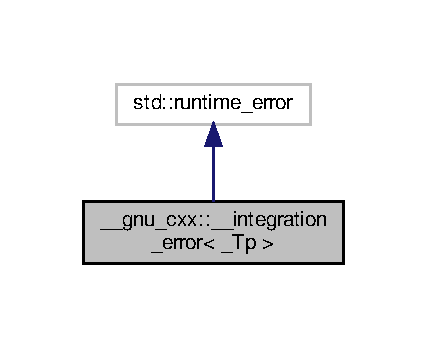
\includegraphics[width=205pt]{class____gnu__cxx_1_1____integration__error__inherit__graph}
\end{center}
\end{figure}


Collaboration diagram for \+\_\+\+\_\+gnu\+\_\+cxx\+:\+:\+\_\+\+\_\+integration\+\_\+error$<$ \+\_\+\+Tp $>$\+:
\nopagebreak
\begin{figure}[H]
\begin{center}
\leavevmode
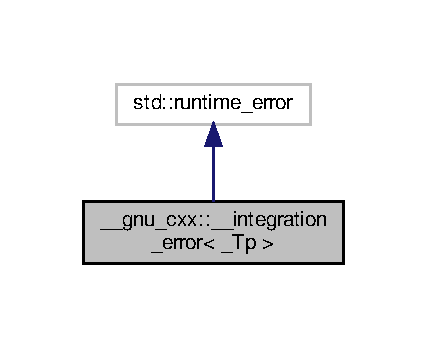
\includegraphics[width=205pt]{class____gnu__cxx_1_1____integration__error__coll__graph}
\end{center}
\end{figure}
\subsection*{Public Member Functions}
\begin{DoxyCompactItemize}
\item 
\hyperlink{class____gnu__cxx_1_1____integration__error_a4a635205d93f9a0c5d3317903c46d3fd}{\+\_\+\+\_\+integration\+\_\+error} (const char $\ast$\+\_\+\+\_\+what, int \+\_\+\+\_\+errcode, \hyperlink{namespace____gnu__cxx_a3b19a9c800ca194374ef9172290f7d79}{\+\_\+\+Tp} \hyperlink{namespace____gnu__cxx_a500ea9f53aeaecd8c2ae657503450578}{\+\_\+\+\_\+result}=std\+::numeric\+\_\+limits$<$ \hyperlink{namespace____gnu__cxx_a3b19a9c800ca194374ef9172290f7d79}{\+\_\+\+Tp} $>$\+::quiet\+\_\+\+NaN(), \hyperlink{namespace____gnu__cxx_a3b19a9c800ca194374ef9172290f7d79}{\+\_\+\+Tp} \hyperlink{namespace____gnu__cxx_a72f736cff127f1574e91a301de9e074b}{\+\_\+\+\_\+abserr}=std\+::numeric\+\_\+limits$<$ \hyperlink{namespace____gnu__cxx_a3b19a9c800ca194374ef9172290f7d79}{\+\_\+\+Tp} $>$\+::quiet\+\_\+\+NaN())
\item 
\hyperlink{namespace____gnu__cxx_a3b19a9c800ca194374ef9172290f7d79}{\+\_\+\+Tp} \hyperlink{class____gnu__cxx_1_1____integration__error_a0194cc847bfbe439a8a1b41cda1d8572}{abserr} () const
\item 
int \hyperlink{class____gnu__cxx_1_1____integration__error_a930f87a4a99140366df637260a2e5929}{error\+\_\+code} () const
\item 
\hyperlink{namespace____gnu__cxx_a3b19a9c800ca194374ef9172290f7d79}{\+\_\+\+Tp} \hyperlink{class____gnu__cxx_1_1____integration__error_abc65cbc56e30b33859f9df92aaf8b636}{result} () const
\end{DoxyCompactItemize}


\subsection{Detailed Description}
\subsubsection*{template$<$typename \+\_\+\+Tp$>$\newline
class \+\_\+\+\_\+gnu\+\_\+cxx\+::\+\_\+\+\_\+integration\+\_\+error$<$ \+\_\+\+Tp $>$}



Definition at line 49 of file integration\+\_\+error.\+h.



\subsection{Constructor \& Destructor Documentation}
\mbox{\Hypertarget{class____gnu__cxx_1_1____integration__error_a4a635205d93f9a0c5d3317903c46d3fd}\label{class____gnu__cxx_1_1____integration__error_a4a635205d93f9a0c5d3317903c46d3fd}} 
\index{\+\_\+\+\_\+gnu\+\_\+cxx\+::\+\_\+\+\_\+integration\+\_\+error@{\+\_\+\+\_\+gnu\+\_\+cxx\+::\+\_\+\+\_\+integration\+\_\+error}!\+\_\+\+\_\+integration\+\_\+error@{\+\_\+\+\_\+integration\+\_\+error}}
\index{\+\_\+\+\_\+integration\+\_\+error@{\+\_\+\+\_\+integration\+\_\+error}!\+\_\+\+\_\+gnu\+\_\+cxx\+::\+\_\+\+\_\+integration\+\_\+error@{\+\_\+\+\_\+gnu\+\_\+cxx\+::\+\_\+\+\_\+integration\+\_\+error}}
\subsubsection{\texorpdfstring{\+\_\+\+\_\+integration\+\_\+error()}{\_\_integration\_error()}}
{\footnotesize\ttfamily template$<$typename \+\_\+\+Tp $>$ \\
\hyperlink{class____gnu__cxx_1_1____integration__error}{\+\_\+\+\_\+gnu\+\_\+cxx\+::\+\_\+\+\_\+integration\+\_\+error}$<$ \hyperlink{namespace____gnu__cxx_a3b19a9c800ca194374ef9172290f7d79}{\+\_\+\+Tp} $>$\+::\hyperlink{class____gnu__cxx_1_1____integration__error}{\+\_\+\+\_\+integration\+\_\+error} (\begin{DoxyParamCaption}\item[{const char $\ast$}]{\+\_\+\+\_\+what,  }\item[{int}]{\+\_\+\+\_\+errcode,  }\item[{\hyperlink{namespace____gnu__cxx_a3b19a9c800ca194374ef9172290f7d79}{\+\_\+\+Tp}}]{\+\_\+\+\_\+result = {\ttfamily std\+:\+:numeric\+\_\+limits$<$\hyperlink{namespace____gnu__cxx_a3b19a9c800ca194374ef9172290f7d79}{\+\_\+\+Tp}$>$\+:\+:quiet\+\_\+NaN()},  }\item[{\hyperlink{namespace____gnu__cxx_a3b19a9c800ca194374ef9172290f7d79}{\+\_\+\+Tp}}]{\+\_\+\+\_\+abserr = {\ttfamily std\+:\+:numeric\+\_\+limits$<$\hyperlink{namespace____gnu__cxx_a3b19a9c800ca194374ef9172290f7d79}{\+\_\+\+Tp}$>$\+:\+:quiet\+\_\+NaN()} }\end{DoxyParamCaption})\hspace{0.3cm}{\ttfamily [inline]}}



Definition at line 57 of file integration\+\_\+error.\+h.



Referenced by \+\_\+\+\_\+gnu\+\_\+cxx\+::\+\_\+\+\_\+throw\+\_\+integration\+\_\+error().


\begin{DoxyCode}
60       : std::runtime\_error(\_\_what),
61         \_M\_result(\hyperlink{namespace____gnu__cxx_a500ea9f53aeaecd8c2ae657503450578}{\_\_result}),
62         \_M\_abserr(\hyperlink{namespace____gnu__cxx_a72f736cff127f1574e91a301de9e074b}{\_\_abserr}),
63         \_M\_errcode(\_\_errcode)
64       \{ \}
\end{DoxyCode}


\subsection{Member Function Documentation}
\mbox{\Hypertarget{class____gnu__cxx_1_1____integration__error_a0194cc847bfbe439a8a1b41cda1d8572}\label{class____gnu__cxx_1_1____integration__error_a0194cc847bfbe439a8a1b41cda1d8572}} 
\index{\+\_\+\+\_\+gnu\+\_\+cxx\+::\+\_\+\+\_\+integration\+\_\+error@{\+\_\+\+\_\+gnu\+\_\+cxx\+::\+\_\+\+\_\+integration\+\_\+error}!abserr@{abserr}}
\index{abserr@{abserr}!\+\_\+\+\_\+gnu\+\_\+cxx\+::\+\_\+\+\_\+integration\+\_\+error@{\+\_\+\+\_\+gnu\+\_\+cxx\+::\+\_\+\+\_\+integration\+\_\+error}}
\subsubsection{\texorpdfstring{abserr()}{abserr()}}
{\footnotesize\ttfamily template$<$typename \+\_\+\+Tp $>$ \\
\hyperlink{namespace____gnu__cxx_a3b19a9c800ca194374ef9172290f7d79}{\+\_\+\+Tp} \hyperlink{class____gnu__cxx_1_1____integration__error}{\+\_\+\+\_\+gnu\+\_\+cxx\+::\+\_\+\+\_\+integration\+\_\+error}$<$ \hyperlink{namespace____gnu__cxx_a3b19a9c800ca194374ef9172290f7d79}{\+\_\+\+Tp} $>$\+::abserr (\begin{DoxyParamCaption}{ }\end{DoxyParamCaption}) const\hspace{0.3cm}{\ttfamily [inline]}}



Definition at line 75 of file integration\+\_\+error.\+h.



References \+\_\+\+\_\+gnu\+\_\+cxx\+::\+\_\+\+\_\+abserr, \+\_\+\+\_\+gnu\+\_\+cxx\+::\+\_\+\+\_\+result, \+\_\+\+\_\+gnu\+\_\+cxx\+::\+\_\+\+\_\+throw\+\_\+integration\+\_\+error(), and \+\_\+\+\_\+gnu\+\_\+cxx\+::\+\_\+\+Tp.


\begin{DoxyCode}
76       \{ \textcolor{keywordflow}{return} this->\_M\_abserr; \}
\end{DoxyCode}
\mbox{\Hypertarget{class____gnu__cxx_1_1____integration__error_a930f87a4a99140366df637260a2e5929}\label{class____gnu__cxx_1_1____integration__error_a930f87a4a99140366df637260a2e5929}} 
\index{\+\_\+\+\_\+gnu\+\_\+cxx\+::\+\_\+\+\_\+integration\+\_\+error@{\+\_\+\+\_\+gnu\+\_\+cxx\+::\+\_\+\+\_\+integration\+\_\+error}!error\+\_\+code@{error\+\_\+code}}
\index{error\+\_\+code@{error\+\_\+code}!\+\_\+\+\_\+gnu\+\_\+cxx\+::\+\_\+\+\_\+integration\+\_\+error@{\+\_\+\+\_\+gnu\+\_\+cxx\+::\+\_\+\+\_\+integration\+\_\+error}}
\subsubsection{\texorpdfstring{error\+\_\+code()}{error\_code()}}
{\footnotesize\ttfamily template$<$typename \+\_\+\+Tp $>$ \\
int \hyperlink{class____gnu__cxx_1_1____integration__error}{\+\_\+\+\_\+gnu\+\_\+cxx\+::\+\_\+\+\_\+integration\+\_\+error}$<$ \hyperlink{namespace____gnu__cxx_a3b19a9c800ca194374ef9172290f7d79}{\+\_\+\+Tp} $>$\+::error\+\_\+code (\begin{DoxyParamCaption}{ }\end{DoxyParamCaption}) const\hspace{0.3cm}{\ttfamily [inline]}}



Definition at line 67 of file integration\+\_\+error.\+h.



References \+\_\+\+\_\+gnu\+\_\+cxx\+::\+\_\+\+Tp.


\begin{DoxyCode}
68       \{ \textcolor{keywordflow}{return} \_M\_errcode; \}
\end{DoxyCode}
\mbox{\Hypertarget{class____gnu__cxx_1_1____integration__error_abc65cbc56e30b33859f9df92aaf8b636}\label{class____gnu__cxx_1_1____integration__error_abc65cbc56e30b33859f9df92aaf8b636}} 
\index{\+\_\+\+\_\+gnu\+\_\+cxx\+::\+\_\+\+\_\+integration\+\_\+error@{\+\_\+\+\_\+gnu\+\_\+cxx\+::\+\_\+\+\_\+integration\+\_\+error}!result@{result}}
\index{result@{result}!\+\_\+\+\_\+gnu\+\_\+cxx\+::\+\_\+\+\_\+integration\+\_\+error@{\+\_\+\+\_\+gnu\+\_\+cxx\+::\+\_\+\+\_\+integration\+\_\+error}}
\subsubsection{\texorpdfstring{result()}{result()}}
{\footnotesize\ttfamily template$<$typename \+\_\+\+Tp $>$ \\
\hyperlink{namespace____gnu__cxx_a3b19a9c800ca194374ef9172290f7d79}{\+\_\+\+Tp} \hyperlink{class____gnu__cxx_1_1____integration__error}{\+\_\+\+\_\+gnu\+\_\+cxx\+::\+\_\+\+\_\+integration\+\_\+error}$<$ \hyperlink{namespace____gnu__cxx_a3b19a9c800ca194374ef9172290f7d79}{\+\_\+\+Tp} $>$\+::result (\begin{DoxyParamCaption}{ }\end{DoxyParamCaption}) const\hspace{0.3cm}{\ttfamily [inline]}}



Definition at line 71 of file integration\+\_\+error.\+h.



References \+\_\+\+\_\+gnu\+\_\+cxx\+::\+\_\+\+Tp.


\begin{DoxyCode}
72       \{ \textcolor{keywordflow}{return} this->\_M\_result; \}
\end{DoxyCode}


The documentation for this class was generated from the following file\+:\begin{DoxyCompactItemize}
\item 
include/ext/\hyperlink{integration__error_8h}{integration\+\_\+error.\+h}\end{DoxyCompactItemize}

\hypertarget{class____gnu__cxx_1_1____phase__iterator}{}\section{\+\_\+\+\_\+gnu\+\_\+cxx\+:\+:\+\_\+\+\_\+phase\+\_\+iterator$<$ \+\_\+\+Tp $>$ Class Template Reference}
\label{class____gnu__cxx_1_1____phase__iterator}\index{\+\_\+\+\_\+gnu\+\_\+cxx\+::\+\_\+\+\_\+phase\+\_\+iterator$<$ \+\_\+\+Tp $>$@{\+\_\+\+\_\+gnu\+\_\+cxx\+::\+\_\+\+\_\+phase\+\_\+iterator$<$ \+\_\+\+Tp $>$}}


{\ttfamily \#include $<$fourier\+\_\+transform.\+h$>$}



Inheritance diagram for \+\_\+\+\_\+gnu\+\_\+cxx\+:\+:\+\_\+\+\_\+phase\+\_\+iterator$<$ \+\_\+\+Tp $>$\+:
\nopagebreak
\begin{figure}[H]
\begin{center}
\leavevmode
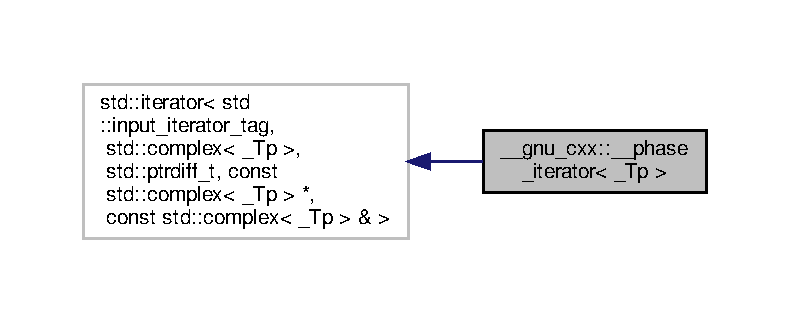
\includegraphics[width=350pt]{class____gnu__cxx_1_1____phase__iterator__inherit__graph}
\end{center}
\end{figure}


Collaboration diagram for \+\_\+\+\_\+gnu\+\_\+cxx\+:\+:\+\_\+\+\_\+phase\+\_\+iterator$<$ \+\_\+\+Tp $>$\+:
\nopagebreak
\begin{figure}[H]
\begin{center}
\leavevmode
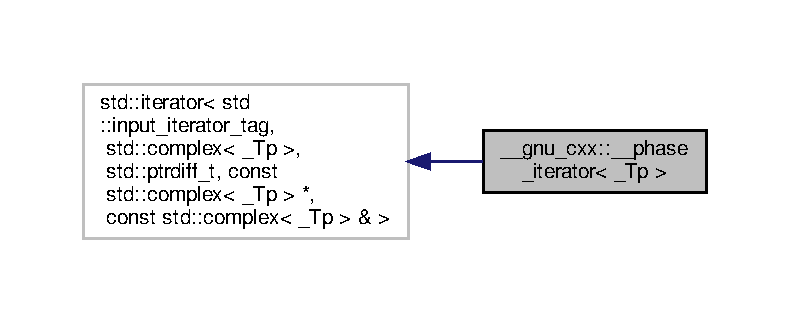
\includegraphics[width=350pt]{class____gnu__cxx_1_1____phase__iterator__coll__graph}
\end{center}
\end{figure}
\subsection*{Public Member Functions}
\begin{DoxyCompactItemize}
\item 
\hyperlink{class____gnu__cxx_1_1____phase__iterator_af39f5fc7df3ea01a383f9bc7345b2330}{\+\_\+\+\_\+phase\+\_\+iterator} (\hyperlink{namespace____gnu__cxx_a3b19a9c800ca194374ef9172290f7d79}{\+\_\+\+Tp} \+\_\+\+\_\+sign, std\+::size\+\_\+t \+\_\+\+\_\+i, std\+::size\+\_\+t \+\_\+\+\_\+len, \hyperlink{namespace____gnu__cxx_ae83aca57f97767d5d09188718728a0ac}{bool} \+\_\+\+\_\+past\+\_\+end=false)
\item 
\hyperlink{class____gnu__cxx_1_1____phase__iterator_af8e0ad92d27e66a746106603aafe9115}{\+\_\+\+\_\+phase\+\_\+iterator} (\hyperlink{namespace____gnu__cxx_a3b19a9c800ca194374ef9172290f7d79}{\+\_\+\+Tp} \+\_\+\+\_\+delta)
\item 
\hyperlink{namespace____gnu__cxx_a3b19a9c800ca194374ef9172290f7d79}{\+\_\+\+Tp} \hyperlink{class____gnu__cxx_1_1____phase__iterator_a4a6cbe9737e8073a586c35d355a89cca}{cos} () const
\item 
\hyperlink{namespace____gnu__cxx_ae83aca57f97767d5d09188718728a0ac}{bool} \hyperlink{class____gnu__cxx_1_1____phase__iterator_ad66a70010229f4a0fe2cea225d59405e}{operator!=} (const \hyperlink{class____gnu__cxx_1_1____phase__iterator}{\+\_\+\+\_\+phase\+\_\+iterator} \&\+\_\+\+\_\+other) const
\item 
std\+::complex$<$ \hyperlink{namespace____gnu__cxx_a3b19a9c800ca194374ef9172290f7d79}{\+\_\+\+Tp} $>$ \hyperlink{class____gnu__cxx_1_1____phase__iterator_afdc5bcce2768619f94cd8da8d0be2a75}{operator$\ast$} () const
\item 
\hyperlink{class____gnu__cxx_1_1____phase__iterator}{\+\_\+\+\_\+phase\+\_\+iterator} \& \hyperlink{class____gnu__cxx_1_1____phase__iterator_a8ef453c6297641600aeacbbeb69e1525}{operator++} ()
\item 
\hyperlink{class____gnu__cxx_1_1____phase__iterator}{\+\_\+\+\_\+phase\+\_\+iterator} \hyperlink{class____gnu__cxx_1_1____phase__iterator_acb438f7faf5843bd8060214874bdcd81}{operator++} (int)
\item 
\hyperlink{namespace____gnu__cxx_ae83aca57f97767d5d09188718728a0ac}{bool} \hyperlink{class____gnu__cxx_1_1____phase__iterator_a8c60a48f50a1646d06c54507ddd6c2b2}{operator==} (const \hyperlink{class____gnu__cxx_1_1____phase__iterator}{\+\_\+\+\_\+phase\+\_\+iterator} \&\+\_\+\+\_\+other) const
\item 
\hyperlink{namespace____gnu__cxx_a3b19a9c800ca194374ef9172290f7d79}{\+\_\+\+Tp} \hyperlink{class____gnu__cxx_1_1____phase__iterator_aaf464df540423bc4d451ca55a93bd9d7}{sin} () const
\end{DoxyCompactItemize}


\subsection{Detailed Description}
\subsubsection*{template$<$typename \+\_\+\+Tp$>$\newline
class \+\_\+\+\_\+gnu\+\_\+cxx\+::\+\_\+\+\_\+phase\+\_\+iterator$<$ \+\_\+\+Tp $>$}



Definition at line 36 of file fourier\+\_\+transform.\+h.



\subsection{Constructor \& Destructor Documentation}
\mbox{\Hypertarget{class____gnu__cxx_1_1____phase__iterator_af39f5fc7df3ea01a383f9bc7345b2330}\label{class____gnu__cxx_1_1____phase__iterator_af39f5fc7df3ea01a383f9bc7345b2330}} 
\index{\+\_\+\+\_\+gnu\+\_\+cxx\+::\+\_\+\+\_\+phase\+\_\+iterator@{\+\_\+\+\_\+gnu\+\_\+cxx\+::\+\_\+\+\_\+phase\+\_\+iterator}!\+\_\+\+\_\+phase\+\_\+iterator@{\+\_\+\+\_\+phase\+\_\+iterator}}
\index{\+\_\+\+\_\+phase\+\_\+iterator@{\+\_\+\+\_\+phase\+\_\+iterator}!\+\_\+\+\_\+gnu\+\_\+cxx\+::\+\_\+\+\_\+phase\+\_\+iterator@{\+\_\+\+\_\+gnu\+\_\+cxx\+::\+\_\+\+\_\+phase\+\_\+iterator}}
\subsubsection{\texorpdfstring{\+\_\+\+\_\+phase\+\_\+iterator()}{\_\_phase\_iterator()}\hspace{0.1cm}{\footnotesize\ttfamily [1/2]}}
{\footnotesize\ttfamily template$<$typename \+\_\+\+Tp $>$ \\
\hyperlink{class____gnu__cxx_1_1____phase__iterator}{\+\_\+\+\_\+gnu\+\_\+cxx\+::\+\_\+\+\_\+phase\+\_\+iterator}$<$ \hyperlink{namespace____gnu__cxx_a3b19a9c800ca194374ef9172290f7d79}{\+\_\+\+Tp} $>$\+::\hyperlink{class____gnu__cxx_1_1____phase__iterator}{\+\_\+\+\_\+phase\+\_\+iterator} (\begin{DoxyParamCaption}\item[{\hyperlink{namespace____gnu__cxx_a3b19a9c800ca194374ef9172290f7d79}{\+\_\+\+Tp}}]{\+\_\+\+\_\+sign,  }\item[{std\+::size\+\_\+t}]{\+\_\+\+\_\+i,  }\item[{std\+::size\+\_\+t}]{\+\_\+\+\_\+len,  }\item[{\hyperlink{namespace____gnu__cxx_ae83aca57f97767d5d09188718728a0ac}{bool}}]{\+\_\+\+\_\+past\+\_\+end = {\ttfamily false} }\end{DoxyParamCaption})\hspace{0.3cm}{\ttfamily [inline]}}



Definition at line 63 of file fourier\+\_\+transform.\+h.



References \+\_\+\+\_\+gnu\+\_\+cxx\+::\+\_\+\+Tp.


\begin{DoxyCode}
67       : \_M\_omega\_pow\_i(std::polar(\hyperlink{namespace____gnu__cxx_a3b19a9c800ca194374ef9172290f7d79}{\_Tp}\{1\},
68                                   -\_\_sign * \_S\_rational\_arg(\_\_i, \_\_len))),
69         \_M\_omega\_pow\_ik(\hyperlink{namespace____gnu__cxx_a3b19a9c800ca194374ef9172290f7d79}{\_Tp}\{1\}),
70         \_M\_k(\_\_past\_end ? \_\_len : 0)
71       \{ \}
\end{DoxyCode}
\mbox{\Hypertarget{class____gnu__cxx_1_1____phase__iterator_af8e0ad92d27e66a746106603aafe9115}\label{class____gnu__cxx_1_1____phase__iterator_af8e0ad92d27e66a746106603aafe9115}} 
\index{\+\_\+\+\_\+gnu\+\_\+cxx\+::\+\_\+\+\_\+phase\+\_\+iterator@{\+\_\+\+\_\+gnu\+\_\+cxx\+::\+\_\+\+\_\+phase\+\_\+iterator}!\+\_\+\+\_\+phase\+\_\+iterator@{\+\_\+\+\_\+phase\+\_\+iterator}}
\index{\+\_\+\+\_\+phase\+\_\+iterator@{\+\_\+\+\_\+phase\+\_\+iterator}!\+\_\+\+\_\+gnu\+\_\+cxx\+::\+\_\+\+\_\+phase\+\_\+iterator@{\+\_\+\+\_\+gnu\+\_\+cxx\+::\+\_\+\+\_\+phase\+\_\+iterator}}
\subsubsection{\texorpdfstring{\+\_\+\+\_\+phase\+\_\+iterator()}{\_\_phase\_iterator()}\hspace{0.1cm}{\footnotesize\ttfamily [2/2]}}
{\footnotesize\ttfamily template$<$typename \+\_\+\+Tp $>$ \\
\hyperlink{class____gnu__cxx_1_1____phase__iterator}{\+\_\+\+\_\+gnu\+\_\+cxx\+::\+\_\+\+\_\+phase\+\_\+iterator}$<$ \hyperlink{namespace____gnu__cxx_a3b19a9c800ca194374ef9172290f7d79}{\+\_\+\+Tp} $>$\+::\hyperlink{class____gnu__cxx_1_1____phase__iterator}{\+\_\+\+\_\+phase\+\_\+iterator} (\begin{DoxyParamCaption}\item[{\hyperlink{namespace____gnu__cxx_a3b19a9c800ca194374ef9172290f7d79}{\+\_\+\+Tp}}]{\+\_\+\+\_\+delta }\end{DoxyParamCaption})\hspace{0.3cm}{\ttfamily [inline]}}



Definition at line 73 of file fourier\+\_\+transform.\+h.



References \+\_\+\+\_\+gnu\+\_\+cxx\+::\+\_\+\+Tp.


\begin{DoxyCode}
74       : \_M\_omega\_pow\_i(std::polar(\hyperlink{namespace____gnu__cxx_a3b19a9c800ca194374ef9172290f7d79}{\_Tp}\{1\}, \_\_delta)),
75         \_M\_omega\_pow\_ik(\hyperlink{namespace____gnu__cxx_a3b19a9c800ca194374ef9172290f7d79}{\_Tp}\{1\}),
76         \_M\_k(0)
77       \{ \}
\end{DoxyCode}


\subsection{Member Function Documentation}
\mbox{\Hypertarget{class____gnu__cxx_1_1____phase__iterator_a4a6cbe9737e8073a586c35d355a89cca}\label{class____gnu__cxx_1_1____phase__iterator_a4a6cbe9737e8073a586c35d355a89cca}} 
\index{\+\_\+\+\_\+gnu\+\_\+cxx\+::\+\_\+\+\_\+phase\+\_\+iterator@{\+\_\+\+\_\+gnu\+\_\+cxx\+::\+\_\+\+\_\+phase\+\_\+iterator}!cos@{cos}}
\index{cos@{cos}!\+\_\+\+\_\+gnu\+\_\+cxx\+::\+\_\+\+\_\+phase\+\_\+iterator@{\+\_\+\+\_\+gnu\+\_\+cxx\+::\+\_\+\+\_\+phase\+\_\+iterator}}
\subsubsection{\texorpdfstring{cos()}{cos()}}
{\footnotesize\ttfamily template$<$typename \+\_\+\+Tp $>$ \\
\hyperlink{namespace____gnu__cxx_a3b19a9c800ca194374ef9172290f7d79}{\+\_\+\+Tp} \hyperlink{class____gnu__cxx_1_1____phase__iterator}{\+\_\+\+\_\+gnu\+\_\+cxx\+::\+\_\+\+\_\+phase\+\_\+iterator}$<$ \hyperlink{namespace____gnu__cxx_a3b19a9c800ca194374ef9172290f7d79}{\+\_\+\+Tp} $>$\+::cos (\begin{DoxyParamCaption}{ }\end{DoxyParamCaption}) const\hspace{0.3cm}{\ttfamily [inline]}}



Definition at line 101 of file fourier\+\_\+transform.\+h.



References \+\_\+\+\_\+gnu\+\_\+cxx\+::\+\_\+\+Tp.


\begin{DoxyCode}
102       \{ \textcolor{keywordflow}{return} std::real(this->\_M\_omega\_pow\_ik); \}
\end{DoxyCode}
\mbox{\Hypertarget{class____gnu__cxx_1_1____phase__iterator_ad66a70010229f4a0fe2cea225d59405e}\label{class____gnu__cxx_1_1____phase__iterator_ad66a70010229f4a0fe2cea225d59405e}} 
\index{\+\_\+\+\_\+gnu\+\_\+cxx\+::\+\_\+\+\_\+phase\+\_\+iterator@{\+\_\+\+\_\+gnu\+\_\+cxx\+::\+\_\+\+\_\+phase\+\_\+iterator}!operator"!=@{operator"!=}}
\index{operator"!=@{operator"!=}!\+\_\+\+\_\+gnu\+\_\+cxx\+::\+\_\+\+\_\+phase\+\_\+iterator@{\+\_\+\+\_\+gnu\+\_\+cxx\+::\+\_\+\+\_\+phase\+\_\+iterator}}
\subsubsection{\texorpdfstring{operator"!=()}{operator!=()}}
{\footnotesize\ttfamily template$<$typename \+\_\+\+Tp $>$ \\
\hyperlink{namespace____gnu__cxx_ae83aca57f97767d5d09188718728a0ac}{bool} \hyperlink{class____gnu__cxx_1_1____phase__iterator}{\+\_\+\+\_\+gnu\+\_\+cxx\+::\+\_\+\+\_\+phase\+\_\+iterator}$<$ \hyperlink{namespace____gnu__cxx_a3b19a9c800ca194374ef9172290f7d79}{\+\_\+\+Tp} $>$\+::operator!= (\begin{DoxyParamCaption}\item[{const \hyperlink{class____gnu__cxx_1_1____phase__iterator}{\+\_\+\+\_\+phase\+\_\+iterator}$<$ \hyperlink{namespace____gnu__cxx_a3b19a9c800ca194374ef9172290f7d79}{\+\_\+\+Tp} $>$ \&}]{\+\_\+\+\_\+other }\end{DoxyParamCaption}) const\hspace{0.3cm}{\ttfamily [inline]}}



Definition at line 116 of file fourier\+\_\+transform.\+h.


\begin{DoxyCode}
117       \{ \textcolor{keywordflow}{return} !(*\textcolor{keyword}{this} == \_\_other); \}
\end{DoxyCode}
\mbox{\Hypertarget{class____gnu__cxx_1_1____phase__iterator_afdc5bcce2768619f94cd8da8d0be2a75}\label{class____gnu__cxx_1_1____phase__iterator_afdc5bcce2768619f94cd8da8d0be2a75}} 
\index{\+\_\+\+\_\+gnu\+\_\+cxx\+::\+\_\+\+\_\+phase\+\_\+iterator@{\+\_\+\+\_\+gnu\+\_\+cxx\+::\+\_\+\+\_\+phase\+\_\+iterator}!operator$\ast$@{operator$\ast$}}
\index{operator$\ast$@{operator$\ast$}!\+\_\+\+\_\+gnu\+\_\+cxx\+::\+\_\+\+\_\+phase\+\_\+iterator@{\+\_\+\+\_\+gnu\+\_\+cxx\+::\+\_\+\+\_\+phase\+\_\+iterator}}
\subsubsection{\texorpdfstring{operator$\ast$()}{operator*()}}
{\footnotesize\ttfamily template$<$typename \+\_\+\+Tp $>$ \\
std\+::complex$<$\hyperlink{namespace____gnu__cxx_a3b19a9c800ca194374ef9172290f7d79}{\+\_\+\+Tp}$>$ \hyperlink{class____gnu__cxx_1_1____phase__iterator}{\+\_\+\+\_\+gnu\+\_\+cxx\+::\+\_\+\+\_\+phase\+\_\+iterator}$<$ \hyperlink{namespace____gnu__cxx_a3b19a9c800ca194374ef9172290f7d79}{\+\_\+\+Tp} $>$\+::operator$\ast$ (\begin{DoxyParamCaption}{ }\end{DoxyParamCaption}) const\hspace{0.3cm}{\ttfamily [inline]}}



Definition at line 80 of file fourier\+\_\+transform.\+h.


\begin{DoxyCode}
81       \{ \textcolor{keywordflow}{return} \_M\_omega\_pow\_ik; \}
\end{DoxyCode}
\mbox{\Hypertarget{class____gnu__cxx_1_1____phase__iterator_a8ef453c6297641600aeacbbeb69e1525}\label{class____gnu__cxx_1_1____phase__iterator_a8ef453c6297641600aeacbbeb69e1525}} 
\index{\+\_\+\+\_\+gnu\+\_\+cxx\+::\+\_\+\+\_\+phase\+\_\+iterator@{\+\_\+\+\_\+gnu\+\_\+cxx\+::\+\_\+\+\_\+phase\+\_\+iterator}!operator++@{operator++}}
\index{operator++@{operator++}!\+\_\+\+\_\+gnu\+\_\+cxx\+::\+\_\+\+\_\+phase\+\_\+iterator@{\+\_\+\+\_\+gnu\+\_\+cxx\+::\+\_\+\+\_\+phase\+\_\+iterator}}
\subsubsection{\texorpdfstring{operator++()}{operator++()}\hspace{0.1cm}{\footnotesize\ttfamily [1/2]}}
{\footnotesize\ttfamily template$<$typename \+\_\+\+Tp $>$ \\
\hyperlink{class____gnu__cxx_1_1____phase__iterator}{\+\_\+\+\_\+phase\+\_\+iterator}\& \hyperlink{class____gnu__cxx_1_1____phase__iterator}{\+\_\+\+\_\+gnu\+\_\+cxx\+::\+\_\+\+\_\+phase\+\_\+iterator}$<$ \hyperlink{namespace____gnu__cxx_a3b19a9c800ca194374ef9172290f7d79}{\+\_\+\+Tp} $>$\+::operator++ (\begin{DoxyParamCaption}{ }\end{DoxyParamCaption})\hspace{0.3cm}{\ttfamily [inline]}}



Definition at line 84 of file fourier\+\_\+transform.\+h.


\begin{DoxyCode}
85       \{
86         ++this->\_M\_k;
87         this->\_M\_omega\_pow\_ik *= this->\_M\_omega\_pow\_i;
88         \textcolor{keywordflow}{return} *\textcolor{keyword}{this};
89       \}
\end{DoxyCode}
\mbox{\Hypertarget{class____gnu__cxx_1_1____phase__iterator_acb438f7faf5843bd8060214874bdcd81}\label{class____gnu__cxx_1_1____phase__iterator_acb438f7faf5843bd8060214874bdcd81}} 
\index{\+\_\+\+\_\+gnu\+\_\+cxx\+::\+\_\+\+\_\+phase\+\_\+iterator@{\+\_\+\+\_\+gnu\+\_\+cxx\+::\+\_\+\+\_\+phase\+\_\+iterator}!operator++@{operator++}}
\index{operator++@{operator++}!\+\_\+\+\_\+gnu\+\_\+cxx\+::\+\_\+\+\_\+phase\+\_\+iterator@{\+\_\+\+\_\+gnu\+\_\+cxx\+::\+\_\+\+\_\+phase\+\_\+iterator}}
\subsubsection{\texorpdfstring{operator++()}{operator++()}\hspace{0.1cm}{\footnotesize\ttfamily [2/2]}}
{\footnotesize\ttfamily template$<$typename \+\_\+\+Tp $>$ \\
\hyperlink{class____gnu__cxx_1_1____phase__iterator}{\+\_\+\+\_\+phase\+\_\+iterator} \hyperlink{class____gnu__cxx_1_1____phase__iterator}{\+\_\+\+\_\+gnu\+\_\+cxx\+::\+\_\+\+\_\+phase\+\_\+iterator}$<$ \hyperlink{namespace____gnu__cxx_a3b19a9c800ca194374ef9172290f7d79}{\+\_\+\+Tp} $>$\+::operator++ (\begin{DoxyParamCaption}\item[{int}]{ }\end{DoxyParamCaption})\hspace{0.3cm}{\ttfamily [inline]}}



Definition at line 92 of file fourier\+\_\+transform.\+h.



References \+\_\+\+\_\+gnu\+\_\+cxx\+::\+\_\+\+Tp.


\begin{DoxyCode}
93       \{
94         \hyperlink{class____gnu__cxx_1_1____phase__iterator_af39f5fc7df3ea01a383f9bc7345b2330}{\_\_phase\_iterator} \_\_dummy(*\textcolor{keyword}{this});
95         ++this->\_M\_k;
96         this->\_M\_omega\_pow\_ik *= this->\_M\_omega\_pow\_i;
97         \textcolor{keywordflow}{return} \_\_dummy;
98       \}
\end{DoxyCode}
\mbox{\Hypertarget{class____gnu__cxx_1_1____phase__iterator_a8c60a48f50a1646d06c54507ddd6c2b2}\label{class____gnu__cxx_1_1____phase__iterator_a8c60a48f50a1646d06c54507ddd6c2b2}} 
\index{\+\_\+\+\_\+gnu\+\_\+cxx\+::\+\_\+\+\_\+phase\+\_\+iterator@{\+\_\+\+\_\+gnu\+\_\+cxx\+::\+\_\+\+\_\+phase\+\_\+iterator}!operator==@{operator==}}
\index{operator==@{operator==}!\+\_\+\+\_\+gnu\+\_\+cxx\+::\+\_\+\+\_\+phase\+\_\+iterator@{\+\_\+\+\_\+gnu\+\_\+cxx\+::\+\_\+\+\_\+phase\+\_\+iterator}}
\subsubsection{\texorpdfstring{operator==()}{operator==()}}
{\footnotesize\ttfamily template$<$typename \+\_\+\+Tp $>$ \\
\hyperlink{namespace____gnu__cxx_ae83aca57f97767d5d09188718728a0ac}{bool} \hyperlink{class____gnu__cxx_1_1____phase__iterator}{\+\_\+\+\_\+gnu\+\_\+cxx\+::\+\_\+\+\_\+phase\+\_\+iterator}$<$ \hyperlink{namespace____gnu__cxx_a3b19a9c800ca194374ef9172290f7d79}{\+\_\+\+Tp} $>$\+::operator== (\begin{DoxyParamCaption}\item[{const \hyperlink{class____gnu__cxx_1_1____phase__iterator}{\+\_\+\+\_\+phase\+\_\+iterator}$<$ \hyperlink{namespace____gnu__cxx_a3b19a9c800ca194374ef9172290f7d79}{\+\_\+\+Tp} $>$ \&}]{\+\_\+\+\_\+other }\end{DoxyParamCaption}) const\hspace{0.3cm}{\ttfamily [inline]}}



Definition at line 109 of file fourier\+\_\+transform.\+h.


\begin{DoxyCode}
110       \{
111         \textcolor{keywordflow}{return} (this->\_M\_omega\_pow\_i == \_\_other.\_M\_omega\_pow\_i)
112             && (this->\_M\_k == \_\_other.\_M\_k);
113       \}
\end{DoxyCode}
\mbox{\Hypertarget{class____gnu__cxx_1_1____phase__iterator_aaf464df540423bc4d451ca55a93bd9d7}\label{class____gnu__cxx_1_1____phase__iterator_aaf464df540423bc4d451ca55a93bd9d7}} 
\index{\+\_\+\+\_\+gnu\+\_\+cxx\+::\+\_\+\+\_\+phase\+\_\+iterator@{\+\_\+\+\_\+gnu\+\_\+cxx\+::\+\_\+\+\_\+phase\+\_\+iterator}!sin@{sin}}
\index{sin@{sin}!\+\_\+\+\_\+gnu\+\_\+cxx\+::\+\_\+\+\_\+phase\+\_\+iterator@{\+\_\+\+\_\+gnu\+\_\+cxx\+::\+\_\+\+\_\+phase\+\_\+iterator}}
\subsubsection{\texorpdfstring{sin()}{sin()}}
{\footnotesize\ttfamily template$<$typename \+\_\+\+Tp $>$ \\
\hyperlink{namespace____gnu__cxx_a3b19a9c800ca194374ef9172290f7d79}{\+\_\+\+Tp} \hyperlink{class____gnu__cxx_1_1____phase__iterator}{\+\_\+\+\_\+gnu\+\_\+cxx\+::\+\_\+\+\_\+phase\+\_\+iterator}$<$ \hyperlink{namespace____gnu__cxx_a3b19a9c800ca194374ef9172290f7d79}{\+\_\+\+Tp} $>$\+::sin (\begin{DoxyParamCaption}{ }\end{DoxyParamCaption}) const\hspace{0.3cm}{\ttfamily [inline]}}



Definition at line 105 of file fourier\+\_\+transform.\+h.


\begin{DoxyCode}
106       \{ \textcolor{keywordflow}{return} std::imag(this->\_M\_omega\_pow\_ik); \}
\end{DoxyCode}


The documentation for this class was generated from the following file\+:\begin{DoxyCompactItemize}
\item 
include/ext/\hyperlink{fourier__transform_8h}{fourier\+\_\+transform.\+h}\end{DoxyCompactItemize}

\hypertarget{struct____gnu__cxx_1_1adaptive__integral__t}{}\section{\+\_\+\+\_\+gnu\+\_\+cxx\+:\+:adaptive\+\_\+integral\+\_\+t$<$ \+\_\+\+Tp, \+\_\+\+Ret\+Tp $>$ Struct Template Reference}
\label{struct____gnu__cxx_1_1adaptive__integral__t}\index{\+\_\+\+\_\+gnu\+\_\+cxx\+::adaptive\+\_\+integral\+\_\+t$<$ \+\_\+\+Tp, \+\_\+\+Ret\+Tp $>$@{\+\_\+\+\_\+gnu\+\_\+cxx\+::adaptive\+\_\+integral\+\_\+t$<$ \+\_\+\+Tp, \+\_\+\+Ret\+Tp $>$}}


{\ttfamily \#include $<$integration.\+h$>$}

\subsection*{Public Types}
\begin{DoxyCompactItemize}
\item 
using \hyperlink{struct____gnu__cxx_1_1adaptive__integral__t_a2da7a99af03e272efd03b876a6b28308}{\+\_\+\+Abs\+Area\+Tp} = decltype(std\+::abs(\hyperlink{struct____gnu__cxx_1_1adaptive__integral__t_a9371ae517b6bff468e44130718d90f8b}{\+\_\+\+Area\+Tp}\{\}))
\item 
using \hyperlink{struct____gnu__cxx_1_1adaptive__integral__t_a9371ae517b6bff468e44130718d90f8b}{\+\_\+\+Area\+Tp} = decltype(\hyperlink{namespace____gnu__cxx_a886e03ece3d53ff7fa6c098a40f93fa5}{\+\_\+\+Ret\+Tp}\{\} $\ast$\hyperlink{namespace____gnu__cxx_a3b19a9c800ca194374ef9172290f7d79}{\+\_\+\+Tp}\{\})
\end{DoxyCompactItemize}
\subsection*{Public Attributes}
\begin{DoxyCompactItemize}
\item 
\hyperlink{struct____gnu__cxx_1_1adaptive__integral__t_a2da7a99af03e272efd03b876a6b28308}{\+\_\+\+Abs\+Area\+Tp} \hyperlink{struct____gnu__cxx_1_1adaptive__integral__t_aa0edf7f036470e8eaaaa1d5e5126d8b3}{\+\_\+\+\_\+abserr} = \hyperlink{struct____gnu__cxx_1_1adaptive__integral__t_a2da7a99af03e272efd03b876a6b28308}{\+\_\+\+Abs\+Area\+Tp}\{\}
\begin{DoxyCompactList}\small\item\em Absolute value of estimated error. \end{DoxyCompactList}\item 
\hyperlink{struct____gnu__cxx_1_1adaptive__integral__t_a9371ae517b6bff468e44130718d90f8b}{\+\_\+\+Area\+Tp} \hyperlink{struct____gnu__cxx_1_1adaptive__integral__t_ab868081e535832031b0e75d0e4d0197d}{\+\_\+\+\_\+result} = \hyperlink{struct____gnu__cxx_1_1adaptive__integral__t_a9371ae517b6bff468e44130718d90f8b}{\+\_\+\+Area\+Tp}\{\}
\begin{DoxyCompactList}\small\item\em Result of the integral. \end{DoxyCompactList}\end{DoxyCompactItemize}


\subsection{Detailed Description}
\subsubsection*{template$<$typename \+\_\+\+Tp, typename \+\_\+\+Ret\+Tp$>$\newline
struct \+\_\+\+\_\+gnu\+\_\+cxx\+::adaptive\+\_\+integral\+\_\+t$<$ \+\_\+\+Tp, \+\_\+\+Ret\+Tp $>$}

The return type for an adaptive integral rule. 

Definition at line 55 of file integration.\+h.



\subsection{Member Typedef Documentation}
\mbox{\Hypertarget{struct____gnu__cxx_1_1adaptive__integral__t_a2da7a99af03e272efd03b876a6b28308}\label{struct____gnu__cxx_1_1adaptive__integral__t_a2da7a99af03e272efd03b876a6b28308}} 
\index{\+\_\+\+\_\+gnu\+\_\+cxx\+::adaptive\+\_\+integral\+\_\+t@{\+\_\+\+\_\+gnu\+\_\+cxx\+::adaptive\+\_\+integral\+\_\+t}!\+\_\+\+Abs\+Area\+Tp@{\+\_\+\+Abs\+Area\+Tp}}
\index{\+\_\+\+Abs\+Area\+Tp@{\+\_\+\+Abs\+Area\+Tp}!\+\_\+\+\_\+gnu\+\_\+cxx\+::adaptive\+\_\+integral\+\_\+t@{\+\_\+\+\_\+gnu\+\_\+cxx\+::adaptive\+\_\+integral\+\_\+t}}
\subsubsection{\texorpdfstring{\+\_\+\+Abs\+Area\+Tp}{\_AbsAreaTp}}
{\footnotesize\ttfamily template$<$typename \+\_\+\+Tp, typename \+\_\+\+Ret\+Tp$>$ \\
using \hyperlink{struct____gnu__cxx_1_1adaptive__integral__t}{\+\_\+\+\_\+gnu\+\_\+cxx\+::adaptive\+\_\+integral\+\_\+t}$<$ \hyperlink{namespace____gnu__cxx_a3b19a9c800ca194374ef9172290f7d79}{\+\_\+\+Tp}, \hyperlink{namespace____gnu__cxx_a886e03ece3d53ff7fa6c098a40f93fa5}{\+\_\+\+Ret\+Tp} $>$\+::\hyperlink{struct____gnu__cxx_1_1adaptive__integral__t_a2da7a99af03e272efd03b876a6b28308}{\+\_\+\+Abs\+Area\+Tp} =  decltype(std\+::abs(\hyperlink{struct____gnu__cxx_1_1adaptive__integral__t_a9371ae517b6bff468e44130718d90f8b}{\+\_\+\+Area\+Tp}\{\}))}



Definition at line 58 of file integration.\+h.

\mbox{\Hypertarget{struct____gnu__cxx_1_1adaptive__integral__t_a9371ae517b6bff468e44130718d90f8b}\label{struct____gnu__cxx_1_1adaptive__integral__t_a9371ae517b6bff468e44130718d90f8b}} 
\index{\+\_\+\+\_\+gnu\+\_\+cxx\+::adaptive\+\_\+integral\+\_\+t@{\+\_\+\+\_\+gnu\+\_\+cxx\+::adaptive\+\_\+integral\+\_\+t}!\+\_\+\+Area\+Tp@{\+\_\+\+Area\+Tp}}
\index{\+\_\+\+Area\+Tp@{\+\_\+\+Area\+Tp}!\+\_\+\+\_\+gnu\+\_\+cxx\+::adaptive\+\_\+integral\+\_\+t@{\+\_\+\+\_\+gnu\+\_\+cxx\+::adaptive\+\_\+integral\+\_\+t}}
\subsubsection{\texorpdfstring{\+\_\+\+Area\+Tp}{\_AreaTp}}
{\footnotesize\ttfamily template$<$typename \+\_\+\+Tp, typename \+\_\+\+Ret\+Tp$>$ \\
using \hyperlink{struct____gnu__cxx_1_1adaptive__integral__t}{\+\_\+\+\_\+gnu\+\_\+cxx\+::adaptive\+\_\+integral\+\_\+t}$<$ \hyperlink{namespace____gnu__cxx_a3b19a9c800ca194374ef9172290f7d79}{\+\_\+\+Tp}, \hyperlink{namespace____gnu__cxx_a886e03ece3d53ff7fa6c098a40f93fa5}{\+\_\+\+Ret\+Tp} $>$\+::\hyperlink{struct____gnu__cxx_1_1adaptive__integral__t_a9371ae517b6bff468e44130718d90f8b}{\+\_\+\+Area\+Tp} =  decltype(\hyperlink{namespace____gnu__cxx_a886e03ece3d53ff7fa6c098a40f93fa5}{\+\_\+\+Ret\+Tp}\{\} $\ast$ \hyperlink{namespace____gnu__cxx_a3b19a9c800ca194374ef9172290f7d79}{\+\_\+\+Tp}\{\})}



Definition at line 57 of file integration.\+h.



\subsection{Member Data Documentation}
\mbox{\Hypertarget{struct____gnu__cxx_1_1adaptive__integral__t_aa0edf7f036470e8eaaaa1d5e5126d8b3}\label{struct____gnu__cxx_1_1adaptive__integral__t_aa0edf7f036470e8eaaaa1d5e5126d8b3}} 
\index{\+\_\+\+\_\+gnu\+\_\+cxx\+::adaptive\+\_\+integral\+\_\+t@{\+\_\+\+\_\+gnu\+\_\+cxx\+::adaptive\+\_\+integral\+\_\+t}!\+\_\+\+\_\+abserr@{\+\_\+\+\_\+abserr}}
\index{\+\_\+\+\_\+abserr@{\+\_\+\+\_\+abserr}!\+\_\+\+\_\+gnu\+\_\+cxx\+::adaptive\+\_\+integral\+\_\+t@{\+\_\+\+\_\+gnu\+\_\+cxx\+::adaptive\+\_\+integral\+\_\+t}}
\subsubsection{\texorpdfstring{\+\_\+\+\_\+abserr}{\_\_abserr}}
{\footnotesize\ttfamily template$<$typename \+\_\+\+Tp, typename \+\_\+\+Ret\+Tp$>$ \\
\hyperlink{struct____gnu__cxx_1_1adaptive__integral__t_a2da7a99af03e272efd03b876a6b28308}{\+\_\+\+Abs\+Area\+Tp} \hyperlink{struct____gnu__cxx_1_1adaptive__integral__t}{\+\_\+\+\_\+gnu\+\_\+cxx\+::adaptive\+\_\+integral\+\_\+t}$<$ \hyperlink{namespace____gnu__cxx_a3b19a9c800ca194374ef9172290f7d79}{\+\_\+\+Tp}, \hyperlink{namespace____gnu__cxx_a886e03ece3d53ff7fa6c098a40f93fa5}{\+\_\+\+Ret\+Tp} $>$\+::\+\_\+\+\_\+abserr = \hyperlink{struct____gnu__cxx_1_1adaptive__integral__t_a2da7a99af03e272efd03b876a6b28308}{\+\_\+\+Abs\+Area\+Tp}\{\}}



Absolute value of estimated error. 



Definition at line 63 of file integration.\+h.

\mbox{\Hypertarget{struct____gnu__cxx_1_1adaptive__integral__t_ab868081e535832031b0e75d0e4d0197d}\label{struct____gnu__cxx_1_1adaptive__integral__t_ab868081e535832031b0e75d0e4d0197d}} 
\index{\+\_\+\+\_\+gnu\+\_\+cxx\+::adaptive\+\_\+integral\+\_\+t@{\+\_\+\+\_\+gnu\+\_\+cxx\+::adaptive\+\_\+integral\+\_\+t}!\+\_\+\+\_\+result@{\+\_\+\+\_\+result}}
\index{\+\_\+\+\_\+result@{\+\_\+\+\_\+result}!\+\_\+\+\_\+gnu\+\_\+cxx\+::adaptive\+\_\+integral\+\_\+t@{\+\_\+\+\_\+gnu\+\_\+cxx\+::adaptive\+\_\+integral\+\_\+t}}
\subsubsection{\texorpdfstring{\+\_\+\+\_\+result}{\_\_result}}
{\footnotesize\ttfamily template$<$typename \+\_\+\+Tp, typename \+\_\+\+Ret\+Tp$>$ \\
\hyperlink{struct____gnu__cxx_1_1adaptive__integral__t_a9371ae517b6bff468e44130718d90f8b}{\+\_\+\+Area\+Tp} \hyperlink{struct____gnu__cxx_1_1adaptive__integral__t}{\+\_\+\+\_\+gnu\+\_\+cxx\+::adaptive\+\_\+integral\+\_\+t}$<$ \hyperlink{namespace____gnu__cxx_a3b19a9c800ca194374ef9172290f7d79}{\+\_\+\+Tp}, \hyperlink{namespace____gnu__cxx_a886e03ece3d53ff7fa6c098a40f93fa5}{\+\_\+\+Ret\+Tp} $>$\+::\+\_\+\+\_\+result = \hyperlink{struct____gnu__cxx_1_1adaptive__integral__t_a9371ae517b6bff468e44130718d90f8b}{\+\_\+\+Area\+Tp}\{\}}



Result of the integral. 



Definition at line 61 of file integration.\+h.



The documentation for this struct was generated from the following file\+:\begin{DoxyCompactItemize}
\item 
include/ext/\hyperlink{integration_8h}{integration.\+h}\end{DoxyCompactItemize}

\hypertarget{struct____gnu__cxx_1_1chebyshev__integral__t}{}\section{\+\_\+\+\_\+gnu\+\_\+cxx\+:\+:chebyshev\+\_\+integral\+\_\+t$<$ \+\_\+\+Ret\+Tp $>$ Struct Template Reference}
\label{struct____gnu__cxx_1_1chebyshev__integral__t}\index{\+\_\+\+\_\+gnu\+\_\+cxx\+::chebyshev\+\_\+integral\+\_\+t$<$ \+\_\+\+Ret\+Tp $>$@{\+\_\+\+\_\+gnu\+\_\+cxx\+::chebyshev\+\_\+integral\+\_\+t$<$ \+\_\+\+Ret\+Tp $>$}}
\subsection*{Public Attributes}
\begin{DoxyCompactItemize}
\item 
std\+::array$<$ \hyperlink{namespace____gnu__cxx_a886e03ece3d53ff7fa6c098a40f93fa5}{\+\_\+\+Ret\+Tp}, 13 $>$ \hyperlink{struct____gnu__cxx_1_1chebyshev__integral__t_abe2450422eb000b28d5446df6bb08c43}{\+\_\+\+\_\+cheb12}
\item 
std\+::array$<$ \hyperlink{namespace____gnu__cxx_a886e03ece3d53ff7fa6c098a40f93fa5}{\+\_\+\+Ret\+Tp}, 25 $>$ \hyperlink{struct____gnu__cxx_1_1chebyshev__integral__t_ad1f7bac86ebf50a99544f265e7b43366}{\+\_\+\+\_\+cheb24}
\end{DoxyCompactItemize}


\subsection{Detailed Description}
\subsubsection*{template$<$typename \+\_\+\+Ret\+Tp$>$\newline
struct \+\_\+\+\_\+gnu\+\_\+cxx\+::chebyshev\+\_\+integral\+\_\+t$<$ \+\_\+\+Ret\+Tp $>$}



Definition at line 30 of file qcheb\+\_\+integrate.\+tcc.



\subsection{Member Data Documentation}
\mbox{\Hypertarget{struct____gnu__cxx_1_1chebyshev__integral__t_abe2450422eb000b28d5446df6bb08c43}\label{struct____gnu__cxx_1_1chebyshev__integral__t_abe2450422eb000b28d5446df6bb08c43}} 
\index{\+\_\+\+\_\+gnu\+\_\+cxx\+::chebyshev\+\_\+integral\+\_\+t@{\+\_\+\+\_\+gnu\+\_\+cxx\+::chebyshev\+\_\+integral\+\_\+t}!\+\_\+\+\_\+cheb12@{\+\_\+\+\_\+cheb12}}
\index{\+\_\+\+\_\+cheb12@{\+\_\+\+\_\+cheb12}!\+\_\+\+\_\+gnu\+\_\+cxx\+::chebyshev\+\_\+integral\+\_\+t@{\+\_\+\+\_\+gnu\+\_\+cxx\+::chebyshev\+\_\+integral\+\_\+t}}
\subsubsection{\texorpdfstring{\+\_\+\+\_\+cheb12}{\_\_cheb12}}
{\footnotesize\ttfamily template$<$typename \+\_\+\+Ret\+Tp$>$ \\
std\+::array$<$\hyperlink{namespace____gnu__cxx_a886e03ece3d53ff7fa6c098a40f93fa5}{\+\_\+\+Ret\+Tp}, 13$>$ \hyperlink{struct____gnu__cxx_1_1chebyshev__integral__t}{\+\_\+\+\_\+gnu\+\_\+cxx\+::chebyshev\+\_\+integral\+\_\+t}$<$ \hyperlink{namespace____gnu__cxx_a886e03ece3d53ff7fa6c098a40f93fa5}{\+\_\+\+Ret\+Tp} $>$\+::\+\_\+\+\_\+cheb12}



Definition at line 32 of file qcheb\+\_\+integrate.\+tcc.



Referenced by \+\_\+\+\_\+gnu\+\_\+cxx\+::qcheb\+\_\+integrate().

\mbox{\Hypertarget{struct____gnu__cxx_1_1chebyshev__integral__t_ad1f7bac86ebf50a99544f265e7b43366}\label{struct____gnu__cxx_1_1chebyshev__integral__t_ad1f7bac86ebf50a99544f265e7b43366}} 
\index{\+\_\+\+\_\+gnu\+\_\+cxx\+::chebyshev\+\_\+integral\+\_\+t@{\+\_\+\+\_\+gnu\+\_\+cxx\+::chebyshev\+\_\+integral\+\_\+t}!\+\_\+\+\_\+cheb24@{\+\_\+\+\_\+cheb24}}
\index{\+\_\+\+\_\+cheb24@{\+\_\+\+\_\+cheb24}!\+\_\+\+\_\+gnu\+\_\+cxx\+::chebyshev\+\_\+integral\+\_\+t@{\+\_\+\+\_\+gnu\+\_\+cxx\+::chebyshev\+\_\+integral\+\_\+t}}
\subsubsection{\texorpdfstring{\+\_\+\+\_\+cheb24}{\_\_cheb24}}
{\footnotesize\ttfamily template$<$typename \+\_\+\+Ret\+Tp$>$ \\
std\+::array$<$\hyperlink{namespace____gnu__cxx_a886e03ece3d53ff7fa6c098a40f93fa5}{\+\_\+\+Ret\+Tp}, 25$>$ \hyperlink{struct____gnu__cxx_1_1chebyshev__integral__t}{\+\_\+\+\_\+gnu\+\_\+cxx\+::chebyshev\+\_\+integral\+\_\+t}$<$ \hyperlink{namespace____gnu__cxx_a886e03ece3d53ff7fa6c098a40f93fa5}{\+\_\+\+Ret\+Tp} $>$\+::\+\_\+\+\_\+cheb24}



Definition at line 33 of file qcheb\+\_\+integrate.\+tcc.



Referenced by \+\_\+\+\_\+gnu\+\_\+cxx\+::qcheb\+\_\+integrate().



The documentation for this struct was generated from the following file\+:\begin{DoxyCompactItemize}
\item 
include/ext/\hyperlink{qcheb__integrate_8tcc}{qcheb\+\_\+integrate.\+tcc}\end{DoxyCompactItemize}

\hypertarget{class____gnu__cxx_1_1composite__midpoint__integral}{}\section{\+\_\+\+\_\+gnu\+\_\+cxx\+:\+:composite\+\_\+midpoint\+\_\+integral$<$ \+\_\+\+Tp, \+\_\+\+Func\+Tp $>$ Class Template Reference}
\label{class____gnu__cxx_1_1composite__midpoint__integral}\index{\+\_\+\+\_\+gnu\+\_\+cxx\+::composite\+\_\+midpoint\+\_\+integral$<$ \+\_\+\+Tp, \+\_\+\+Func\+Tp $>$@{\+\_\+\+\_\+gnu\+\_\+cxx\+::composite\+\_\+midpoint\+\_\+integral$<$ \+\_\+\+Tp, \+\_\+\+Func\+Tp $>$}}


{\ttfamily \#include $<$midpoint\+\_\+integral.\+h$>$}

\subsection*{Public Types}
\begin{DoxyCompactItemize}
\item 
using \hyperlink{class____gnu__cxx_1_1composite__midpoint__integral_a7b1fb3ea8fc30b6099cea19948fda4a9}{\+\_\+\+Abs\+Area\+Tp} = decltype(std\+::abs(\hyperlink{class____gnu__cxx_1_1composite__midpoint__integral_a02175286c06db2fab6f727eab5117b25}{\+\_\+\+Area\+Tp}\{\}))
\item 
using \hyperlink{class____gnu__cxx_1_1composite__midpoint__integral_a02175286c06db2fab6f727eab5117b25}{\+\_\+\+Area\+Tp} = decltype(\hyperlink{class____gnu__cxx_1_1composite__midpoint__integral_a092b0a129f0d5cd5f7a82d58f8117f94}{\+\_\+\+Ret\+Tp}\{\} $\ast$\hyperlink{namespace____gnu__cxx_a3b19a9c800ca194374ef9172290f7d79}{\+\_\+\+Tp}\{\})
\item 
using \hyperlink{class____gnu__cxx_1_1composite__midpoint__integral_a092b0a129f0d5cd5f7a82d58f8117f94}{\+\_\+\+Ret\+Tp} = std\+::invoke\+\_\+result\+\_\+t$<$ \+\_\+\+Func\+Tp, \hyperlink{namespace____gnu__cxx_a3b19a9c800ca194374ef9172290f7d79}{\+\_\+\+Tp} $>$
\end{DoxyCompactItemize}
\subsection*{Public Member Functions}
\begin{DoxyCompactItemize}
\item 
\hyperlink{class____gnu__cxx_1_1composite__midpoint__integral_a298a54b9f6c71969b28f8b7216d0a78a}{composite\+\_\+midpoint\+\_\+integral} (\+\_\+\+Func\+Tp \+\_\+\+\_\+fun, \hyperlink{namespace____gnu__cxx_a3b19a9c800ca194374ef9172290f7d79}{\+\_\+\+Tp} \+\_\+\+\_\+a, \hyperlink{namespace____gnu__cxx_a3b19a9c800ca194374ef9172290f7d79}{\+\_\+\+Tp} \+\_\+\+\_\+b, std\+::size\+\_\+t \+\_\+\+\_\+num\+\_\+segs)
\item 
{\footnotesize template$<$typename \+\_\+\+Func\+Tp2 $>$ }\\\hyperlink{struct____gnu__cxx_1_1fixed__integral__t}{fixed\+\_\+integral\+\_\+t}$<$ \hyperlink{namespace____gnu__cxx_a3b19a9c800ca194374ef9172290f7d79}{\+\_\+\+Tp}, std\+::invoke\+\_\+result\+\_\+t$<$ \+\_\+\+Func\+Tp2, \hyperlink{namespace____gnu__cxx_a3b19a9c800ca194374ef9172290f7d79}{\+\_\+\+Tp} $>$ $>$ \hyperlink{class____gnu__cxx_1_1composite__midpoint__integral_a7eb1aeb6fba86c8c4dce818b83af4d2d}{integrate} (\+\_\+\+Func\+Tp2 \+\_\+\+\_\+fun, \hyperlink{namespace____gnu__cxx_a3b19a9c800ca194374ef9172290f7d79}{\+\_\+\+Tp} \+\_\+\+\_\+a, \hyperlink{namespace____gnu__cxx_a3b19a9c800ca194374ef9172290f7d79}{\+\_\+\+Tp} \+\_\+\+\_\+b)
\item 
\hyperlink{class____gnu__cxx_1_1composite__midpoint__integral_a02175286c06db2fab6f727eab5117b25}{\+\_\+\+Area\+Tp} \hyperlink{class____gnu__cxx_1_1composite__midpoint__integral_a28788cf79367faecd19fb307925223d0}{operator()} ()
\end{DoxyCompactItemize}


\subsection{Detailed Description}
\subsubsection*{template$<$typename \+\_\+\+Tp, typename \+\_\+\+Func\+Tp$>$\newline
class \+\_\+\+\_\+gnu\+\_\+cxx\+::composite\+\_\+midpoint\+\_\+integral$<$ \+\_\+\+Tp, \+\_\+\+Func\+Tp $>$}



Definition at line 34 of file midpoint\+\_\+integral.\+h.



\subsection{Member Typedef Documentation}
\mbox{\Hypertarget{class____gnu__cxx_1_1composite__midpoint__integral_a7b1fb3ea8fc30b6099cea19948fda4a9}\label{class____gnu__cxx_1_1composite__midpoint__integral_a7b1fb3ea8fc30b6099cea19948fda4a9}} 
\index{\+\_\+\+\_\+gnu\+\_\+cxx\+::composite\+\_\+midpoint\+\_\+integral@{\+\_\+\+\_\+gnu\+\_\+cxx\+::composite\+\_\+midpoint\+\_\+integral}!\+\_\+\+Abs\+Area\+Tp@{\+\_\+\+Abs\+Area\+Tp}}
\index{\+\_\+\+Abs\+Area\+Tp@{\+\_\+\+Abs\+Area\+Tp}!\+\_\+\+\_\+gnu\+\_\+cxx\+::composite\+\_\+midpoint\+\_\+integral@{\+\_\+\+\_\+gnu\+\_\+cxx\+::composite\+\_\+midpoint\+\_\+integral}}
\subsubsection{\texorpdfstring{\+\_\+\+Abs\+Area\+Tp}{\_AbsAreaTp}}
{\footnotesize\ttfamily template$<$typename \+\_\+\+Tp, typename \+\_\+\+Func\+Tp$>$ \\
using \hyperlink{class____gnu__cxx_1_1composite__midpoint__integral}{\+\_\+\+\_\+gnu\+\_\+cxx\+::composite\+\_\+midpoint\+\_\+integral}$<$ \hyperlink{namespace____gnu__cxx_a3b19a9c800ca194374ef9172290f7d79}{\+\_\+\+Tp}, \+\_\+\+Func\+Tp $>$\+::\hyperlink{class____gnu__cxx_1_1composite__midpoint__integral_a7b1fb3ea8fc30b6099cea19948fda4a9}{\+\_\+\+Abs\+Area\+Tp} =  decltype(std\+::abs(\hyperlink{class____gnu__cxx_1_1composite__midpoint__integral_a02175286c06db2fab6f727eab5117b25}{\+\_\+\+Area\+Tp}\{\}))}



Definition at line 40 of file midpoint\+\_\+integral.\+h.

\mbox{\Hypertarget{class____gnu__cxx_1_1composite__midpoint__integral_a02175286c06db2fab6f727eab5117b25}\label{class____gnu__cxx_1_1composite__midpoint__integral_a02175286c06db2fab6f727eab5117b25}} 
\index{\+\_\+\+\_\+gnu\+\_\+cxx\+::composite\+\_\+midpoint\+\_\+integral@{\+\_\+\+\_\+gnu\+\_\+cxx\+::composite\+\_\+midpoint\+\_\+integral}!\+\_\+\+Area\+Tp@{\+\_\+\+Area\+Tp}}
\index{\+\_\+\+Area\+Tp@{\+\_\+\+Area\+Tp}!\+\_\+\+\_\+gnu\+\_\+cxx\+::composite\+\_\+midpoint\+\_\+integral@{\+\_\+\+\_\+gnu\+\_\+cxx\+::composite\+\_\+midpoint\+\_\+integral}}
\subsubsection{\texorpdfstring{\+\_\+\+Area\+Tp}{\_AreaTp}}
{\footnotesize\ttfamily template$<$typename \+\_\+\+Tp, typename \+\_\+\+Func\+Tp$>$ \\
using \hyperlink{class____gnu__cxx_1_1composite__midpoint__integral}{\+\_\+\+\_\+gnu\+\_\+cxx\+::composite\+\_\+midpoint\+\_\+integral}$<$ \hyperlink{namespace____gnu__cxx_a3b19a9c800ca194374ef9172290f7d79}{\+\_\+\+Tp}, \+\_\+\+Func\+Tp $>$\+::\hyperlink{class____gnu__cxx_1_1composite__midpoint__integral_a02175286c06db2fab6f727eab5117b25}{\+\_\+\+Area\+Tp} =  decltype(\hyperlink{class____gnu__cxx_1_1composite__midpoint__integral_a092b0a129f0d5cd5f7a82d58f8117f94}{\+\_\+\+Ret\+Tp}\{\} $\ast$ \hyperlink{namespace____gnu__cxx_a3b19a9c800ca194374ef9172290f7d79}{\+\_\+\+Tp}\{\})}



Definition at line 39 of file midpoint\+\_\+integral.\+h.

\mbox{\Hypertarget{class____gnu__cxx_1_1composite__midpoint__integral_a092b0a129f0d5cd5f7a82d58f8117f94}\label{class____gnu__cxx_1_1composite__midpoint__integral_a092b0a129f0d5cd5f7a82d58f8117f94}} 
\index{\+\_\+\+\_\+gnu\+\_\+cxx\+::composite\+\_\+midpoint\+\_\+integral@{\+\_\+\+\_\+gnu\+\_\+cxx\+::composite\+\_\+midpoint\+\_\+integral}!\+\_\+\+Ret\+Tp@{\+\_\+\+Ret\+Tp}}
\index{\+\_\+\+Ret\+Tp@{\+\_\+\+Ret\+Tp}!\+\_\+\+\_\+gnu\+\_\+cxx\+::composite\+\_\+midpoint\+\_\+integral@{\+\_\+\+\_\+gnu\+\_\+cxx\+::composite\+\_\+midpoint\+\_\+integral}}
\subsubsection{\texorpdfstring{\+\_\+\+Ret\+Tp}{\_RetTp}}
{\footnotesize\ttfamily template$<$typename \+\_\+\+Tp, typename \+\_\+\+Func\+Tp$>$ \\
using \hyperlink{class____gnu__cxx_1_1composite__midpoint__integral}{\+\_\+\+\_\+gnu\+\_\+cxx\+::composite\+\_\+midpoint\+\_\+integral}$<$ \hyperlink{namespace____gnu__cxx_a3b19a9c800ca194374ef9172290f7d79}{\+\_\+\+Tp}, \+\_\+\+Func\+Tp $>$\+::\hyperlink{class____gnu__cxx_1_1composite__midpoint__integral_a092b0a129f0d5cd5f7a82d58f8117f94}{\+\_\+\+Ret\+Tp} =  std\+::invoke\+\_\+result\+\_\+t$<$\+\_\+\+Func\+Tp, \hyperlink{namespace____gnu__cxx_a3b19a9c800ca194374ef9172290f7d79}{\+\_\+\+Tp}$>$}



Definition at line 38 of file midpoint\+\_\+integral.\+h.



\subsection{Constructor \& Destructor Documentation}
\mbox{\Hypertarget{class____gnu__cxx_1_1composite__midpoint__integral_a298a54b9f6c71969b28f8b7216d0a78a}\label{class____gnu__cxx_1_1composite__midpoint__integral_a298a54b9f6c71969b28f8b7216d0a78a}} 
\index{\+\_\+\+\_\+gnu\+\_\+cxx\+::composite\+\_\+midpoint\+\_\+integral@{\+\_\+\+\_\+gnu\+\_\+cxx\+::composite\+\_\+midpoint\+\_\+integral}!composite\+\_\+midpoint\+\_\+integral@{composite\+\_\+midpoint\+\_\+integral}}
\index{composite\+\_\+midpoint\+\_\+integral@{composite\+\_\+midpoint\+\_\+integral}!\+\_\+\+\_\+gnu\+\_\+cxx\+::composite\+\_\+midpoint\+\_\+integral@{\+\_\+\+\_\+gnu\+\_\+cxx\+::composite\+\_\+midpoint\+\_\+integral}}
\subsubsection{\texorpdfstring{composite\+\_\+midpoint\+\_\+integral()}{composite\_midpoint\_integral()}}
{\footnotesize\ttfamily template$<$typename \+\_\+\+Tp, typename \+\_\+\+Func\+Tp$>$ \\
\hyperlink{class____gnu__cxx_1_1composite__midpoint__integral}{\+\_\+\+\_\+gnu\+\_\+cxx\+::composite\+\_\+midpoint\+\_\+integral}$<$ \hyperlink{namespace____gnu__cxx_a3b19a9c800ca194374ef9172290f7d79}{\+\_\+\+Tp}, \+\_\+\+Func\+Tp $>$\+::\hyperlink{class____gnu__cxx_1_1composite__midpoint__integral}{composite\+\_\+midpoint\+\_\+integral} (\begin{DoxyParamCaption}\item[{\+\_\+\+Func\+Tp}]{\+\_\+\+\_\+fun,  }\item[{\hyperlink{namespace____gnu__cxx_a3b19a9c800ca194374ef9172290f7d79}{\+\_\+\+Tp}}]{\+\_\+\+\_\+a,  }\item[{\hyperlink{namespace____gnu__cxx_a3b19a9c800ca194374ef9172290f7d79}{\+\_\+\+Tp}}]{\+\_\+\+\_\+b,  }\item[{std\+::size\+\_\+t}]{\+\_\+\+\_\+num\+\_\+segs }\end{DoxyParamCaption})\hspace{0.3cm}{\ttfamily [inline]}}



Definition at line 42 of file midpoint\+\_\+integral.\+h.



References \+\_\+\+\_\+gnu\+\_\+cxx\+::composite\+\_\+midpoint\+\_\+integral$<$ \+\_\+\+Tp, \+\_\+\+Func\+Tp $>$\+::operator()().


\begin{DoxyCode}
44       : \_M\_fun(\_\_fun), \_M\_lower\_lim(\_\_a), \_M\_upper\_lim(\_\_b),
45         \_M\_num\_segs(\_\_num\_segs), \_M\_result()
46       \{ \}
\end{DoxyCode}


\subsection{Member Function Documentation}
\mbox{\Hypertarget{class____gnu__cxx_1_1composite__midpoint__integral_a7eb1aeb6fba86c8c4dce818b83af4d2d}\label{class____gnu__cxx_1_1composite__midpoint__integral_a7eb1aeb6fba86c8c4dce818b83af4d2d}} 
\index{\+\_\+\+\_\+gnu\+\_\+cxx\+::composite\+\_\+midpoint\+\_\+integral@{\+\_\+\+\_\+gnu\+\_\+cxx\+::composite\+\_\+midpoint\+\_\+integral}!integrate@{integrate}}
\index{integrate@{integrate}!\+\_\+\+\_\+gnu\+\_\+cxx\+::composite\+\_\+midpoint\+\_\+integral@{\+\_\+\+\_\+gnu\+\_\+cxx\+::composite\+\_\+midpoint\+\_\+integral}}
\subsubsection{\texorpdfstring{integrate()}{integrate()}}
{\footnotesize\ttfamily template$<$typename \+\_\+\+Tp, typename \+\_\+\+Func\+Tp$>$ \\
template$<$typename \+\_\+\+Func\+Tp2 $>$ \\
\hyperlink{struct____gnu__cxx_1_1fixed__integral__t}{fixed\+\_\+integral\+\_\+t}$<$\hyperlink{namespace____gnu__cxx_a3b19a9c800ca194374ef9172290f7d79}{\+\_\+\+Tp}, std\+::invoke\+\_\+result\+\_\+t$<$\+\_\+\+Func\+Tp2, \hyperlink{namespace____gnu__cxx_a3b19a9c800ca194374ef9172290f7d79}{\+\_\+\+Tp}$>$ $>$ \hyperlink{class____gnu__cxx_1_1composite__midpoint__integral}{\+\_\+\+\_\+gnu\+\_\+cxx\+::composite\+\_\+midpoint\+\_\+integral}$<$ \hyperlink{namespace____gnu__cxx_a3b19a9c800ca194374ef9172290f7d79}{\+\_\+\+Tp}, \+\_\+\+Func\+Tp $>$\+::integrate (\begin{DoxyParamCaption}\item[{\+\_\+\+Func\+Tp2}]{\+\_\+\+\_\+fun,  }\item[{\hyperlink{namespace____gnu__cxx_a3b19a9c800ca194374ef9172290f7d79}{\+\_\+\+Tp}}]{\+\_\+\+\_\+a,  }\item[{\hyperlink{namespace____gnu__cxx_a3b19a9c800ca194374ef9172290f7d79}{\+\_\+\+Tp}}]{\+\_\+\+\_\+b }\end{DoxyParamCaption})\hspace{0.3cm}{\ttfamily [inline]}}



Definition at line 52 of file midpoint\+\_\+integral.\+h.



References \+\_\+\+\_\+gnu\+\_\+cxx\+::\+\_\+\+Tp.



Referenced by \+\_\+\+\_\+gnu\+\_\+cxx\+::midpoint\+\_\+integral$<$ \+\_\+\+Tp, \+\_\+\+Func\+Tp $>$\+::operator()().


\begin{DoxyCode}
53         \{
54           composite\_midpoint\_integral<\_FuncTp2, \_Tp>
55             \_\_trapi(\_\_fun, \_\_a, \_\_b, this->\_M\_num\_segments);
56           \textcolor{keywordflow}{return} \{\_\_trapi()\};
57         \}
\end{DoxyCode}
\mbox{\Hypertarget{class____gnu__cxx_1_1composite__midpoint__integral_a28788cf79367faecd19fb307925223d0}\label{class____gnu__cxx_1_1composite__midpoint__integral_a28788cf79367faecd19fb307925223d0}} 
\index{\+\_\+\+\_\+gnu\+\_\+cxx\+::composite\+\_\+midpoint\+\_\+integral@{\+\_\+\+\_\+gnu\+\_\+cxx\+::composite\+\_\+midpoint\+\_\+integral}!operator()@{operator()}}
\index{operator()@{operator()}!\+\_\+\+\_\+gnu\+\_\+cxx\+::composite\+\_\+midpoint\+\_\+integral@{\+\_\+\+\_\+gnu\+\_\+cxx\+::composite\+\_\+midpoint\+\_\+integral}}
\subsubsection{\texorpdfstring{operator()()}{operator()()}}
{\footnotesize\ttfamily template$<$typename \+\_\+\+Tp , typename \+\_\+\+Func\+Tp $>$ \\
\hyperlink{class____gnu__cxx_1_1composite__midpoint__integral}{composite\+\_\+midpoint\+\_\+integral}$<$ \hyperlink{namespace____gnu__cxx_a3b19a9c800ca194374ef9172290f7d79}{\+\_\+\+Tp}, \+\_\+\+Func\+Tp $>$\+::\hyperlink{class____gnu__cxx_1_1composite__midpoint__integral_a02175286c06db2fab6f727eab5117b25}{\+\_\+\+Area\+Tp} \hyperlink{class____gnu__cxx_1_1composite__midpoint__integral}{\+\_\+\+\_\+gnu\+\_\+cxx\+::composite\+\_\+midpoint\+\_\+integral}$<$ \hyperlink{namespace____gnu__cxx_a3b19a9c800ca194374ef9172290f7d79}{\+\_\+\+Tp}, \+\_\+\+Func\+Tp $>$\+::operator() (\begin{DoxyParamCaption}{ }\end{DoxyParamCaption})}

Integrate the function by naive subdivision. 

Definition at line 33 of file midpoint\+\_\+integral.\+tcc.



References \+\_\+\+\_\+gnu\+\_\+cxx\+::\+\_\+\+Tp.



Referenced by \+\_\+\+\_\+gnu\+\_\+cxx\+::composite\+\_\+midpoint\+\_\+integral$<$ \+\_\+\+Tp, \+\_\+\+Func\+Tp $>$\+::composite\+\_\+midpoint\+\_\+integral(), and \+\_\+\+\_\+gnu\+\_\+cxx\+::midpoint\+\_\+integral$<$ \+\_\+\+Tp, \+\_\+\+Func\+Tp $>$\+::midpoint\+\_\+integral().


\begin{DoxyCode}
34     \{
35       \textcolor{keyword}{const} \textcolor{keyword}{auto} \_\_delta = (this->\_M\_upper\_lim - this->\_M\_lower\_lim)
36                            / this->\_M\_num\_segs;
37 
38       \textcolor{keyword}{auto} \_\_sum = this->\_M\_fun(this->\_M\_lower\_lim + \_\_delta / \hyperlink{namespace____gnu__cxx_a3b19a9c800ca194374ef9172290f7d79}{\_Tp}\{2\}) / \hyperlink{namespace____gnu__cxx_a3b19a9c800ca194374ef9172290f7d79}{\_Tp}\{2\};
39       \textcolor{keywordflow}{for} (std::size\_t \_\_j = 1; \_\_j < this->\_M\_num\_segs; ++\_\_j)
40         \_\_sum += this->\_M\_fun(this->\_M\_lower\_lim + \hyperlink{namespace____gnu__cxx_a3b19a9c800ca194374ef9172290f7d79}{\_Tp}(\_\_j + 0.5) * \_\_delta);
41 
42       this->\_M\_result = \_\_sum * \_\_delta;
43 
44       \textcolor{keywordflow}{return} this->\_M\_result;
45     \}
\end{DoxyCode}


The documentation for this class was generated from the following files\+:\begin{DoxyCompactItemize}
\item 
include/ext/\hyperlink{midpoint__integral_8h}{midpoint\+\_\+integral.\+h}\item 
include/ext/\hyperlink{midpoint__integral_8tcc}{midpoint\+\_\+integral.\+tcc}\end{DoxyCompactItemize}

\hypertarget{class____gnu__cxx_1_1composite__simpson__integral}{}\section{\+\_\+\+\_\+gnu\+\_\+cxx\+:\+:composite\+\_\+simpson\+\_\+integral$<$ \+\_\+\+Tp, \+\_\+\+Func\+Tp $>$ Class Template Reference}
\label{class____gnu__cxx_1_1composite__simpson__integral}\index{\+\_\+\+\_\+gnu\+\_\+cxx\+::composite\+\_\+simpson\+\_\+integral$<$ \+\_\+\+Tp, \+\_\+\+Func\+Tp $>$@{\+\_\+\+\_\+gnu\+\_\+cxx\+::composite\+\_\+simpson\+\_\+integral$<$ \+\_\+\+Tp, \+\_\+\+Func\+Tp $>$}}


{\ttfamily \#include $<$simpson\+\_\+integral.\+h$>$}

\subsection*{Public Types}
\begin{DoxyCompactItemize}
\item 
using \hyperlink{class____gnu__cxx_1_1composite__simpson__integral_a7057fa13b914730f021356f761b6c448}{\+\_\+\+Abs\+Area\+Tp} = decltype(std\+::abs(\hyperlink{class____gnu__cxx_1_1composite__simpson__integral_a1a3ef5313bafc1d8523f2d517b066a7a}{\+\_\+\+Area\+Tp}\{\}))
\item 
using \hyperlink{class____gnu__cxx_1_1composite__simpson__integral_a1a3ef5313bafc1d8523f2d517b066a7a}{\+\_\+\+Area\+Tp} = decltype(\hyperlink{class____gnu__cxx_1_1composite__simpson__integral_a530008576c8a3a786e84ccbd96c93cc5}{\+\_\+\+Ret\+Tp}\{\} $\ast$\hyperlink{namespace____gnu__cxx_a3b19a9c800ca194374ef9172290f7d79}{\+\_\+\+Tp}\{\})
\item 
using \hyperlink{class____gnu__cxx_1_1composite__simpson__integral_a530008576c8a3a786e84ccbd96c93cc5}{\+\_\+\+Ret\+Tp} = std\+::invoke\+\_\+result\+\_\+t$<$ \+\_\+\+Func\+Tp, \hyperlink{namespace____gnu__cxx_a3b19a9c800ca194374ef9172290f7d79}{\+\_\+\+Tp} $>$
\end{DoxyCompactItemize}
\subsection*{Public Member Functions}
\begin{DoxyCompactItemize}
\item 
\hyperlink{class____gnu__cxx_1_1composite__simpson__integral_a1348464cb4681d828755d647c513aba7}{composite\+\_\+simpson\+\_\+integral} (\+\_\+\+Func\+Tp \+\_\+\+\_\+fun, \hyperlink{namespace____gnu__cxx_a3b19a9c800ca194374ef9172290f7d79}{\+\_\+\+Tp} \+\_\+\+\_\+a, \hyperlink{namespace____gnu__cxx_a3b19a9c800ca194374ef9172290f7d79}{\+\_\+\+Tp} \+\_\+\+\_\+b, std\+::size\+\_\+t \+\_\+\+\_\+num\+\_\+segs)
\item 
{\footnotesize template$<$typename \+\_\+\+Func\+Tp2 $>$ }\\\hyperlink{struct____gnu__cxx_1_1fixed__integral__t}{fixed\+\_\+integral\+\_\+t}$<$ \hyperlink{namespace____gnu__cxx_a3b19a9c800ca194374ef9172290f7d79}{\+\_\+\+Tp}, std\+::invoke\+\_\+result\+\_\+t$<$ \+\_\+\+Func\+Tp2, \hyperlink{namespace____gnu__cxx_a3b19a9c800ca194374ef9172290f7d79}{\+\_\+\+Tp} $>$ $>$ \hyperlink{class____gnu__cxx_1_1composite__simpson__integral_a932c3e6ea25f340113955340dbec54c0}{integrate} (\+\_\+\+Func\+Tp2 \+\_\+\+\_\+fun, \hyperlink{namespace____gnu__cxx_a3b19a9c800ca194374ef9172290f7d79}{\+\_\+\+Tp} \+\_\+\+\_\+a, \hyperlink{namespace____gnu__cxx_a3b19a9c800ca194374ef9172290f7d79}{\+\_\+\+Tp} \+\_\+\+\_\+b)
\item 
\hyperlink{class____gnu__cxx_1_1composite__simpson__integral_a1a3ef5313bafc1d8523f2d517b066a7a}{\+\_\+\+Area\+Tp} \hyperlink{class____gnu__cxx_1_1composite__simpson__integral_a7c60338016d2c10eddc8bd9b8dfd3264}{operator()} ()
\end{DoxyCompactItemize}


\subsection{Detailed Description}
\subsubsection*{template$<$typename \+\_\+\+Tp, typename \+\_\+\+Func\+Tp$>$\newline
class \+\_\+\+\_\+gnu\+\_\+cxx\+::composite\+\_\+simpson\+\_\+integral$<$ \+\_\+\+Tp, \+\_\+\+Func\+Tp $>$}



Definition at line 34 of file simpson\+\_\+integral.\+h.



\subsection{Member Typedef Documentation}
\mbox{\Hypertarget{class____gnu__cxx_1_1composite__simpson__integral_a7057fa13b914730f021356f761b6c448}\label{class____gnu__cxx_1_1composite__simpson__integral_a7057fa13b914730f021356f761b6c448}} 
\index{\+\_\+\+\_\+gnu\+\_\+cxx\+::composite\+\_\+simpson\+\_\+integral@{\+\_\+\+\_\+gnu\+\_\+cxx\+::composite\+\_\+simpson\+\_\+integral}!\+\_\+\+Abs\+Area\+Tp@{\+\_\+\+Abs\+Area\+Tp}}
\index{\+\_\+\+Abs\+Area\+Tp@{\+\_\+\+Abs\+Area\+Tp}!\+\_\+\+\_\+gnu\+\_\+cxx\+::composite\+\_\+simpson\+\_\+integral@{\+\_\+\+\_\+gnu\+\_\+cxx\+::composite\+\_\+simpson\+\_\+integral}}
\subsubsection{\texorpdfstring{\+\_\+\+Abs\+Area\+Tp}{\_AbsAreaTp}}
{\footnotesize\ttfamily template$<$typename \+\_\+\+Tp, typename \+\_\+\+Func\+Tp$>$ \\
using \hyperlink{class____gnu__cxx_1_1composite__simpson__integral}{\+\_\+\+\_\+gnu\+\_\+cxx\+::composite\+\_\+simpson\+\_\+integral}$<$ \hyperlink{namespace____gnu__cxx_a3b19a9c800ca194374ef9172290f7d79}{\+\_\+\+Tp}, \+\_\+\+Func\+Tp $>$\+::\hyperlink{class____gnu__cxx_1_1composite__simpson__integral_a7057fa13b914730f021356f761b6c448}{\+\_\+\+Abs\+Area\+Tp} =  decltype(std\+::abs(\hyperlink{class____gnu__cxx_1_1composite__simpson__integral_a1a3ef5313bafc1d8523f2d517b066a7a}{\+\_\+\+Area\+Tp}\{\}))}



Definition at line 40 of file simpson\+\_\+integral.\+h.

\mbox{\Hypertarget{class____gnu__cxx_1_1composite__simpson__integral_a1a3ef5313bafc1d8523f2d517b066a7a}\label{class____gnu__cxx_1_1composite__simpson__integral_a1a3ef5313bafc1d8523f2d517b066a7a}} 
\index{\+\_\+\+\_\+gnu\+\_\+cxx\+::composite\+\_\+simpson\+\_\+integral@{\+\_\+\+\_\+gnu\+\_\+cxx\+::composite\+\_\+simpson\+\_\+integral}!\+\_\+\+Area\+Tp@{\+\_\+\+Area\+Tp}}
\index{\+\_\+\+Area\+Tp@{\+\_\+\+Area\+Tp}!\+\_\+\+\_\+gnu\+\_\+cxx\+::composite\+\_\+simpson\+\_\+integral@{\+\_\+\+\_\+gnu\+\_\+cxx\+::composite\+\_\+simpson\+\_\+integral}}
\subsubsection{\texorpdfstring{\+\_\+\+Area\+Tp}{\_AreaTp}}
{\footnotesize\ttfamily template$<$typename \+\_\+\+Tp, typename \+\_\+\+Func\+Tp$>$ \\
using \hyperlink{class____gnu__cxx_1_1composite__simpson__integral}{\+\_\+\+\_\+gnu\+\_\+cxx\+::composite\+\_\+simpson\+\_\+integral}$<$ \hyperlink{namespace____gnu__cxx_a3b19a9c800ca194374ef9172290f7d79}{\+\_\+\+Tp}, \+\_\+\+Func\+Tp $>$\+::\hyperlink{class____gnu__cxx_1_1composite__simpson__integral_a1a3ef5313bafc1d8523f2d517b066a7a}{\+\_\+\+Area\+Tp} =  decltype(\hyperlink{class____gnu__cxx_1_1composite__simpson__integral_a530008576c8a3a786e84ccbd96c93cc5}{\+\_\+\+Ret\+Tp}\{\} $\ast$ \hyperlink{namespace____gnu__cxx_a3b19a9c800ca194374ef9172290f7d79}{\+\_\+\+Tp}\{\})}



Definition at line 39 of file simpson\+\_\+integral.\+h.

\mbox{\Hypertarget{class____gnu__cxx_1_1composite__simpson__integral_a530008576c8a3a786e84ccbd96c93cc5}\label{class____gnu__cxx_1_1composite__simpson__integral_a530008576c8a3a786e84ccbd96c93cc5}} 
\index{\+\_\+\+\_\+gnu\+\_\+cxx\+::composite\+\_\+simpson\+\_\+integral@{\+\_\+\+\_\+gnu\+\_\+cxx\+::composite\+\_\+simpson\+\_\+integral}!\+\_\+\+Ret\+Tp@{\+\_\+\+Ret\+Tp}}
\index{\+\_\+\+Ret\+Tp@{\+\_\+\+Ret\+Tp}!\+\_\+\+\_\+gnu\+\_\+cxx\+::composite\+\_\+simpson\+\_\+integral@{\+\_\+\+\_\+gnu\+\_\+cxx\+::composite\+\_\+simpson\+\_\+integral}}
\subsubsection{\texorpdfstring{\+\_\+\+Ret\+Tp}{\_RetTp}}
{\footnotesize\ttfamily template$<$typename \+\_\+\+Tp, typename \+\_\+\+Func\+Tp$>$ \\
using \hyperlink{class____gnu__cxx_1_1composite__simpson__integral}{\+\_\+\+\_\+gnu\+\_\+cxx\+::composite\+\_\+simpson\+\_\+integral}$<$ \hyperlink{namespace____gnu__cxx_a3b19a9c800ca194374ef9172290f7d79}{\+\_\+\+Tp}, \+\_\+\+Func\+Tp $>$\+::\hyperlink{class____gnu__cxx_1_1composite__simpson__integral_a530008576c8a3a786e84ccbd96c93cc5}{\+\_\+\+Ret\+Tp} =  std\+::invoke\+\_\+result\+\_\+t$<$\+\_\+\+Func\+Tp, \hyperlink{namespace____gnu__cxx_a3b19a9c800ca194374ef9172290f7d79}{\+\_\+\+Tp}$>$}



Definition at line 38 of file simpson\+\_\+integral.\+h.



\subsection{Constructor \& Destructor Documentation}
\mbox{\Hypertarget{class____gnu__cxx_1_1composite__simpson__integral_a1348464cb4681d828755d647c513aba7}\label{class____gnu__cxx_1_1composite__simpson__integral_a1348464cb4681d828755d647c513aba7}} 
\index{\+\_\+\+\_\+gnu\+\_\+cxx\+::composite\+\_\+simpson\+\_\+integral@{\+\_\+\+\_\+gnu\+\_\+cxx\+::composite\+\_\+simpson\+\_\+integral}!composite\+\_\+simpson\+\_\+integral@{composite\+\_\+simpson\+\_\+integral}}
\index{composite\+\_\+simpson\+\_\+integral@{composite\+\_\+simpson\+\_\+integral}!\+\_\+\+\_\+gnu\+\_\+cxx\+::composite\+\_\+simpson\+\_\+integral@{\+\_\+\+\_\+gnu\+\_\+cxx\+::composite\+\_\+simpson\+\_\+integral}}
\subsubsection{\texorpdfstring{composite\+\_\+simpson\+\_\+integral()}{composite\_simpson\_integral()}}
{\footnotesize\ttfamily template$<$typename \+\_\+\+Tp, typename \+\_\+\+Func\+Tp$>$ \\
\hyperlink{class____gnu__cxx_1_1composite__simpson__integral}{\+\_\+\+\_\+gnu\+\_\+cxx\+::composite\+\_\+simpson\+\_\+integral}$<$ \hyperlink{namespace____gnu__cxx_a3b19a9c800ca194374ef9172290f7d79}{\+\_\+\+Tp}, \+\_\+\+Func\+Tp $>$\+::\hyperlink{class____gnu__cxx_1_1composite__simpson__integral}{composite\+\_\+simpson\+\_\+integral} (\begin{DoxyParamCaption}\item[{\+\_\+\+Func\+Tp}]{\+\_\+\+\_\+fun,  }\item[{\hyperlink{namespace____gnu__cxx_a3b19a9c800ca194374ef9172290f7d79}{\+\_\+\+Tp}}]{\+\_\+\+\_\+a,  }\item[{\hyperlink{namespace____gnu__cxx_a3b19a9c800ca194374ef9172290f7d79}{\+\_\+\+Tp}}]{\+\_\+\+\_\+b,  }\item[{std\+::size\+\_\+t}]{\+\_\+\+\_\+num\+\_\+segs }\end{DoxyParamCaption})\hspace{0.3cm}{\ttfamily [inline]}}



Definition at line 42 of file simpson\+\_\+integral.\+h.



References \+\_\+\+\_\+gnu\+\_\+cxx\+::composite\+\_\+simpson\+\_\+integral$<$ \+\_\+\+Tp, \+\_\+\+Func\+Tp $>$\+::operator()().


\begin{DoxyCode}
44       : \_M\_fun(\_\_fun), \_M\_lower\_lim(\_\_a), \_M\_upper\_lim(\_\_b),
45         \_M\_num\_segs(\_\_num\_segs), \_M\_result()
46       \{ \}
\end{DoxyCode}


\subsection{Member Function Documentation}
\mbox{\Hypertarget{class____gnu__cxx_1_1composite__simpson__integral_a932c3e6ea25f340113955340dbec54c0}\label{class____gnu__cxx_1_1composite__simpson__integral_a932c3e6ea25f340113955340dbec54c0}} 
\index{\+\_\+\+\_\+gnu\+\_\+cxx\+::composite\+\_\+simpson\+\_\+integral@{\+\_\+\+\_\+gnu\+\_\+cxx\+::composite\+\_\+simpson\+\_\+integral}!integrate@{integrate}}
\index{integrate@{integrate}!\+\_\+\+\_\+gnu\+\_\+cxx\+::composite\+\_\+simpson\+\_\+integral@{\+\_\+\+\_\+gnu\+\_\+cxx\+::composite\+\_\+simpson\+\_\+integral}}
\subsubsection{\texorpdfstring{integrate()}{integrate()}}
{\footnotesize\ttfamily template$<$typename \+\_\+\+Tp, typename \+\_\+\+Func\+Tp$>$ \\
template$<$typename \+\_\+\+Func\+Tp2 $>$ \\
\hyperlink{struct____gnu__cxx_1_1fixed__integral__t}{fixed\+\_\+integral\+\_\+t}$<$\hyperlink{namespace____gnu__cxx_a3b19a9c800ca194374ef9172290f7d79}{\+\_\+\+Tp}, std\+::invoke\+\_\+result\+\_\+t$<$\+\_\+\+Func\+Tp2, \hyperlink{namespace____gnu__cxx_a3b19a9c800ca194374ef9172290f7d79}{\+\_\+\+Tp}$>$ $>$ \hyperlink{class____gnu__cxx_1_1composite__simpson__integral}{\+\_\+\+\_\+gnu\+\_\+cxx\+::composite\+\_\+simpson\+\_\+integral}$<$ \hyperlink{namespace____gnu__cxx_a3b19a9c800ca194374ef9172290f7d79}{\+\_\+\+Tp}, \+\_\+\+Func\+Tp $>$\+::integrate (\begin{DoxyParamCaption}\item[{\+\_\+\+Func\+Tp2}]{\+\_\+\+\_\+fun,  }\item[{\hyperlink{namespace____gnu__cxx_a3b19a9c800ca194374ef9172290f7d79}{\+\_\+\+Tp}}]{\+\_\+\+\_\+a,  }\item[{\hyperlink{namespace____gnu__cxx_a3b19a9c800ca194374ef9172290f7d79}{\+\_\+\+Tp}}]{\+\_\+\+\_\+b }\end{DoxyParamCaption})\hspace{0.3cm}{\ttfamily [inline]}}



Definition at line 52 of file simpson\+\_\+integral.\+h.



References \+\_\+\+\_\+gnu\+\_\+cxx\+::\+\_\+\+Tp.



Referenced by \+\_\+\+\_\+gnu\+\_\+cxx\+::simpson\+\_\+integral$<$ \+\_\+\+Tp, \+\_\+\+Func\+Tp $>$\+::operator()().


\begin{DoxyCode}
53         \{
54           composite\_simpson\_integral<\_FuncTp2, \_Tp>
55             \_\_trapi(\_\_fun, \_\_a, \_\_b, this->\_M\_num\_segments);
56           \textcolor{keywordflow}{return} \{\_\_trapi()\};
57         \}
\end{DoxyCode}
\mbox{\Hypertarget{class____gnu__cxx_1_1composite__simpson__integral_a7c60338016d2c10eddc8bd9b8dfd3264}\label{class____gnu__cxx_1_1composite__simpson__integral_a7c60338016d2c10eddc8bd9b8dfd3264}} 
\index{\+\_\+\+\_\+gnu\+\_\+cxx\+::composite\+\_\+simpson\+\_\+integral@{\+\_\+\+\_\+gnu\+\_\+cxx\+::composite\+\_\+simpson\+\_\+integral}!operator()@{operator()}}
\index{operator()@{operator()}!\+\_\+\+\_\+gnu\+\_\+cxx\+::composite\+\_\+simpson\+\_\+integral@{\+\_\+\+\_\+gnu\+\_\+cxx\+::composite\+\_\+simpson\+\_\+integral}}
\subsubsection{\texorpdfstring{operator()()}{operator()()}}
{\footnotesize\ttfamily template$<$typename \+\_\+\+Tp , typename \+\_\+\+Func\+Tp $>$ \\
\hyperlink{class____gnu__cxx_1_1composite__simpson__integral}{composite\+\_\+simpson\+\_\+integral}$<$ \hyperlink{namespace____gnu__cxx_a3b19a9c800ca194374ef9172290f7d79}{\+\_\+\+Tp}, \+\_\+\+Func\+Tp $>$\+::\hyperlink{class____gnu__cxx_1_1composite__simpson__integral_a1a3ef5313bafc1d8523f2d517b066a7a}{\+\_\+\+Area\+Tp} \hyperlink{class____gnu__cxx_1_1composite__simpson__integral}{\+\_\+\+\_\+gnu\+\_\+cxx\+::composite\+\_\+simpson\+\_\+integral}$<$ \hyperlink{namespace____gnu__cxx_a3b19a9c800ca194374ef9172290f7d79}{\+\_\+\+Tp}, \+\_\+\+Func\+Tp $>$\+::operator() (\begin{DoxyParamCaption}{ }\end{DoxyParamCaption})}

Integrate the function by naive subdivision. 

Definition at line 33 of file simpson\+\_\+integral.\+tcc.



References \+\_\+\+\_\+gnu\+\_\+cxx\+::\+\_\+\+Tp.



Referenced by \+\_\+\+\_\+gnu\+\_\+cxx\+::composite\+\_\+simpson\+\_\+integral$<$ \+\_\+\+Tp, \+\_\+\+Func\+Tp $>$\+::composite\+\_\+simpson\+\_\+integral(), and \+\_\+\+\_\+gnu\+\_\+cxx\+::simpson\+\_\+integral$<$ \+\_\+\+Tp, \+\_\+\+Func\+Tp $>$\+::simpson\+\_\+integral().


\begin{DoxyCode}
34     \{
35       \textcolor{keyword}{const} \textcolor{keyword}{auto} \_\_delta = (this->\_M\_upper\_lim - this->\_M\_lower\_lim)
36                            / this->\_M\_num\_segs / 2;
37 
38       \textcolor{keyword}{auto} \_\_x = this->\_M\_lower\_lim;
39       \textcolor{keyword}{auto} \_\_sum = this->\_M\_fun(\_\_x);
40       \_\_x += \_\_delta;
41       \_\_sum += \hyperlink{namespace____gnu__cxx_a3b19a9c800ca194374ef9172290f7d79}{\_Tp}\{2\} * this->\_M\_fun(\_\_x);
42       \textcolor{keywordflow}{for} (std::size\_t \_\_j = 1; \_\_j < this->\_M\_num\_segs; ++\_\_j)
43         \{
44           \_\_x += \_\_delta;
45           \_\_sum += \hyperlink{namespace____gnu__cxx_a3b19a9c800ca194374ef9172290f7d79}{\_Tp}\{4\} * this->\_M\_fun(\_\_x);
46           \_\_x += \_\_delta;
47           \_\_sum += \hyperlink{namespace____gnu__cxx_a3b19a9c800ca194374ef9172290f7d79}{\_Tp}\{2\} * this->\_M\_fun(\_\_x);
48         \}
49       \_\_sum += this->\_M\_fun(this->\_M\_upper\_lim);
50 
51       this->\_M\_result = \_\_sum * \_\_delta / \hyperlink{namespace____gnu__cxx_a3b19a9c800ca194374ef9172290f7d79}{\_Tp}\{6\};
52 
53       \textcolor{keywordflow}{return} this->\_M\_result;
54     \}
\end{DoxyCode}


The documentation for this class was generated from the following files\+:\begin{DoxyCompactItemize}
\item 
include/ext/\hyperlink{simpson__integral_8h}{simpson\+\_\+integral.\+h}\item 
include/ext/\hyperlink{simpson__integral_8tcc}{simpson\+\_\+integral.\+tcc}\end{DoxyCompactItemize}

\hypertarget{class____gnu__cxx_1_1composite__trapezoid__integral}{}\section{\+\_\+\+\_\+gnu\+\_\+cxx\+:\+:composite\+\_\+trapezoid\+\_\+integral$<$ \+\_\+\+Tp, \+\_\+\+Func\+Tp $>$ Class Template Reference}
\label{class____gnu__cxx_1_1composite__trapezoid__integral}\index{\+\_\+\+\_\+gnu\+\_\+cxx\+::composite\+\_\+trapezoid\+\_\+integral$<$ \+\_\+\+Tp, \+\_\+\+Func\+Tp $>$@{\+\_\+\+\_\+gnu\+\_\+cxx\+::composite\+\_\+trapezoid\+\_\+integral$<$ \+\_\+\+Tp, \+\_\+\+Func\+Tp $>$}}


{\ttfamily \#include $<$trapezoid\+\_\+integral.\+h$>$}

\subsection*{Public Types}
\begin{DoxyCompactItemize}
\item 
using \hyperlink{class____gnu__cxx_1_1composite__trapezoid__integral_a3e05f617e964dd6ec4ae2e42c600c1a7}{\+\_\+\+Abs\+Area\+Tp} = decltype(std\+::abs(\hyperlink{class____gnu__cxx_1_1composite__trapezoid__integral_a0839ba042e2636869679bbf343b2a930}{\+\_\+\+Area\+Tp}\{\}))
\item 
using \hyperlink{class____gnu__cxx_1_1composite__trapezoid__integral_a0839ba042e2636869679bbf343b2a930}{\+\_\+\+Area\+Tp} = decltype(\hyperlink{class____gnu__cxx_1_1composite__trapezoid__integral_af223f0ed55e750221cb3114c6f2fcb60}{\+\_\+\+Ret\+Tp}\{\} $\ast$\hyperlink{namespace____gnu__cxx_a3b19a9c800ca194374ef9172290f7d79}{\+\_\+\+Tp}\{\})
\item 
using \hyperlink{class____gnu__cxx_1_1composite__trapezoid__integral_af223f0ed55e750221cb3114c6f2fcb60}{\+\_\+\+Ret\+Tp} = std\+::invoke\+\_\+result\+\_\+t$<$ \+\_\+\+Func\+Tp, \hyperlink{namespace____gnu__cxx_a3b19a9c800ca194374ef9172290f7d79}{\+\_\+\+Tp} $>$
\end{DoxyCompactItemize}
\subsection*{Public Member Functions}
\begin{DoxyCompactItemize}
\item 
\hyperlink{class____gnu__cxx_1_1composite__trapezoid__integral_a168c2e7ecd8c89e87cc308e756c486ed}{composite\+\_\+trapezoid\+\_\+integral} (\+\_\+\+Func\+Tp \+\_\+\+\_\+fun, \hyperlink{namespace____gnu__cxx_a3b19a9c800ca194374ef9172290f7d79}{\+\_\+\+Tp} \+\_\+\+\_\+a, \hyperlink{namespace____gnu__cxx_a3b19a9c800ca194374ef9172290f7d79}{\+\_\+\+Tp} \+\_\+\+\_\+b, std\+::size\+\_\+t \+\_\+\+\_\+num\+\_\+segs)
\item 
{\footnotesize template$<$typename \+\_\+\+Func\+Tp2 $>$ }\\\hyperlink{struct____gnu__cxx_1_1fixed__integral__t}{fixed\+\_\+integral\+\_\+t}$<$ \hyperlink{namespace____gnu__cxx_a3b19a9c800ca194374ef9172290f7d79}{\+\_\+\+Tp}, std\+::invoke\+\_\+result\+\_\+t$<$ \+\_\+\+Func\+Tp2, \hyperlink{namespace____gnu__cxx_a3b19a9c800ca194374ef9172290f7d79}{\+\_\+\+Tp} $>$ $>$ \hyperlink{class____gnu__cxx_1_1composite__trapezoid__integral_a8897329b7ae73a8e41028519fab78b81}{integrate} (\+\_\+\+Func\+Tp2 \+\_\+\+\_\+fun, \hyperlink{namespace____gnu__cxx_a3b19a9c800ca194374ef9172290f7d79}{\+\_\+\+Tp} \+\_\+\+\_\+a, \hyperlink{namespace____gnu__cxx_a3b19a9c800ca194374ef9172290f7d79}{\+\_\+\+Tp} \+\_\+\+\_\+b)
\item 
\hyperlink{class____gnu__cxx_1_1composite__trapezoid__integral_a0839ba042e2636869679bbf343b2a930}{\+\_\+\+Area\+Tp} \hyperlink{class____gnu__cxx_1_1composite__trapezoid__integral_aad283e15b63ce1ad40cdaa834ec4fcb6}{operator()} ()
\end{DoxyCompactItemize}


\subsection{Detailed Description}
\subsubsection*{template$<$typename \+\_\+\+Tp, typename \+\_\+\+Func\+Tp$>$\newline
class \+\_\+\+\_\+gnu\+\_\+cxx\+::composite\+\_\+trapezoid\+\_\+integral$<$ \+\_\+\+Tp, \+\_\+\+Func\+Tp $>$}



Definition at line 34 of file trapezoid\+\_\+integral.\+h.



\subsection{Member Typedef Documentation}
\mbox{\Hypertarget{class____gnu__cxx_1_1composite__trapezoid__integral_a3e05f617e964dd6ec4ae2e42c600c1a7}\label{class____gnu__cxx_1_1composite__trapezoid__integral_a3e05f617e964dd6ec4ae2e42c600c1a7}} 
\index{\+\_\+\+\_\+gnu\+\_\+cxx\+::composite\+\_\+trapezoid\+\_\+integral@{\+\_\+\+\_\+gnu\+\_\+cxx\+::composite\+\_\+trapezoid\+\_\+integral}!\+\_\+\+Abs\+Area\+Tp@{\+\_\+\+Abs\+Area\+Tp}}
\index{\+\_\+\+Abs\+Area\+Tp@{\+\_\+\+Abs\+Area\+Tp}!\+\_\+\+\_\+gnu\+\_\+cxx\+::composite\+\_\+trapezoid\+\_\+integral@{\+\_\+\+\_\+gnu\+\_\+cxx\+::composite\+\_\+trapezoid\+\_\+integral}}
\subsubsection{\texorpdfstring{\+\_\+\+Abs\+Area\+Tp}{\_AbsAreaTp}}
{\footnotesize\ttfamily template$<$typename \+\_\+\+Tp, typename \+\_\+\+Func\+Tp$>$ \\
using \hyperlink{class____gnu__cxx_1_1composite__trapezoid__integral}{\+\_\+\+\_\+gnu\+\_\+cxx\+::composite\+\_\+trapezoid\+\_\+integral}$<$ \hyperlink{namespace____gnu__cxx_a3b19a9c800ca194374ef9172290f7d79}{\+\_\+\+Tp}, \+\_\+\+Func\+Tp $>$\+::\hyperlink{class____gnu__cxx_1_1composite__trapezoid__integral_a3e05f617e964dd6ec4ae2e42c600c1a7}{\+\_\+\+Abs\+Area\+Tp} =  decltype(std\+::abs(\hyperlink{class____gnu__cxx_1_1composite__trapezoid__integral_a0839ba042e2636869679bbf343b2a930}{\+\_\+\+Area\+Tp}\{\}))}



Definition at line 40 of file trapezoid\+\_\+integral.\+h.

\mbox{\Hypertarget{class____gnu__cxx_1_1composite__trapezoid__integral_a0839ba042e2636869679bbf343b2a930}\label{class____gnu__cxx_1_1composite__trapezoid__integral_a0839ba042e2636869679bbf343b2a930}} 
\index{\+\_\+\+\_\+gnu\+\_\+cxx\+::composite\+\_\+trapezoid\+\_\+integral@{\+\_\+\+\_\+gnu\+\_\+cxx\+::composite\+\_\+trapezoid\+\_\+integral}!\+\_\+\+Area\+Tp@{\+\_\+\+Area\+Tp}}
\index{\+\_\+\+Area\+Tp@{\+\_\+\+Area\+Tp}!\+\_\+\+\_\+gnu\+\_\+cxx\+::composite\+\_\+trapezoid\+\_\+integral@{\+\_\+\+\_\+gnu\+\_\+cxx\+::composite\+\_\+trapezoid\+\_\+integral}}
\subsubsection{\texorpdfstring{\+\_\+\+Area\+Tp}{\_AreaTp}}
{\footnotesize\ttfamily template$<$typename \+\_\+\+Tp, typename \+\_\+\+Func\+Tp$>$ \\
using \hyperlink{class____gnu__cxx_1_1composite__trapezoid__integral}{\+\_\+\+\_\+gnu\+\_\+cxx\+::composite\+\_\+trapezoid\+\_\+integral}$<$ \hyperlink{namespace____gnu__cxx_a3b19a9c800ca194374ef9172290f7d79}{\+\_\+\+Tp}, \+\_\+\+Func\+Tp $>$\+::\hyperlink{class____gnu__cxx_1_1composite__trapezoid__integral_a0839ba042e2636869679bbf343b2a930}{\+\_\+\+Area\+Tp} =  decltype(\hyperlink{class____gnu__cxx_1_1composite__trapezoid__integral_af223f0ed55e750221cb3114c6f2fcb60}{\+\_\+\+Ret\+Tp}\{\} $\ast$ \hyperlink{namespace____gnu__cxx_a3b19a9c800ca194374ef9172290f7d79}{\+\_\+\+Tp}\{\})}



Definition at line 39 of file trapezoid\+\_\+integral.\+h.

\mbox{\Hypertarget{class____gnu__cxx_1_1composite__trapezoid__integral_af223f0ed55e750221cb3114c6f2fcb60}\label{class____gnu__cxx_1_1composite__trapezoid__integral_af223f0ed55e750221cb3114c6f2fcb60}} 
\index{\+\_\+\+\_\+gnu\+\_\+cxx\+::composite\+\_\+trapezoid\+\_\+integral@{\+\_\+\+\_\+gnu\+\_\+cxx\+::composite\+\_\+trapezoid\+\_\+integral}!\+\_\+\+Ret\+Tp@{\+\_\+\+Ret\+Tp}}
\index{\+\_\+\+Ret\+Tp@{\+\_\+\+Ret\+Tp}!\+\_\+\+\_\+gnu\+\_\+cxx\+::composite\+\_\+trapezoid\+\_\+integral@{\+\_\+\+\_\+gnu\+\_\+cxx\+::composite\+\_\+trapezoid\+\_\+integral}}
\subsubsection{\texorpdfstring{\+\_\+\+Ret\+Tp}{\_RetTp}}
{\footnotesize\ttfamily template$<$typename \+\_\+\+Tp, typename \+\_\+\+Func\+Tp$>$ \\
using \hyperlink{class____gnu__cxx_1_1composite__trapezoid__integral}{\+\_\+\+\_\+gnu\+\_\+cxx\+::composite\+\_\+trapezoid\+\_\+integral}$<$ \hyperlink{namespace____gnu__cxx_a3b19a9c800ca194374ef9172290f7d79}{\+\_\+\+Tp}, \+\_\+\+Func\+Tp $>$\+::\hyperlink{class____gnu__cxx_1_1composite__trapezoid__integral_af223f0ed55e750221cb3114c6f2fcb60}{\+\_\+\+Ret\+Tp} =  std\+::invoke\+\_\+result\+\_\+t$<$\+\_\+\+Func\+Tp, \hyperlink{namespace____gnu__cxx_a3b19a9c800ca194374ef9172290f7d79}{\+\_\+\+Tp}$>$}



Definition at line 38 of file trapezoid\+\_\+integral.\+h.



\subsection{Constructor \& Destructor Documentation}
\mbox{\Hypertarget{class____gnu__cxx_1_1composite__trapezoid__integral_a168c2e7ecd8c89e87cc308e756c486ed}\label{class____gnu__cxx_1_1composite__trapezoid__integral_a168c2e7ecd8c89e87cc308e756c486ed}} 
\index{\+\_\+\+\_\+gnu\+\_\+cxx\+::composite\+\_\+trapezoid\+\_\+integral@{\+\_\+\+\_\+gnu\+\_\+cxx\+::composite\+\_\+trapezoid\+\_\+integral}!composite\+\_\+trapezoid\+\_\+integral@{composite\+\_\+trapezoid\+\_\+integral}}
\index{composite\+\_\+trapezoid\+\_\+integral@{composite\+\_\+trapezoid\+\_\+integral}!\+\_\+\+\_\+gnu\+\_\+cxx\+::composite\+\_\+trapezoid\+\_\+integral@{\+\_\+\+\_\+gnu\+\_\+cxx\+::composite\+\_\+trapezoid\+\_\+integral}}
\subsubsection{\texorpdfstring{composite\+\_\+trapezoid\+\_\+integral()}{composite\_trapezoid\_integral()}}
{\footnotesize\ttfamily template$<$typename \+\_\+\+Tp, typename \+\_\+\+Func\+Tp$>$ \\
\hyperlink{class____gnu__cxx_1_1composite__trapezoid__integral}{\+\_\+\+\_\+gnu\+\_\+cxx\+::composite\+\_\+trapezoid\+\_\+integral}$<$ \hyperlink{namespace____gnu__cxx_a3b19a9c800ca194374ef9172290f7d79}{\+\_\+\+Tp}, \+\_\+\+Func\+Tp $>$\+::\hyperlink{class____gnu__cxx_1_1composite__trapezoid__integral}{composite\+\_\+trapezoid\+\_\+integral} (\begin{DoxyParamCaption}\item[{\+\_\+\+Func\+Tp}]{\+\_\+\+\_\+fun,  }\item[{\hyperlink{namespace____gnu__cxx_a3b19a9c800ca194374ef9172290f7d79}{\+\_\+\+Tp}}]{\+\_\+\+\_\+a,  }\item[{\hyperlink{namespace____gnu__cxx_a3b19a9c800ca194374ef9172290f7d79}{\+\_\+\+Tp}}]{\+\_\+\+\_\+b,  }\item[{std\+::size\+\_\+t}]{\+\_\+\+\_\+num\+\_\+segs }\end{DoxyParamCaption})\hspace{0.3cm}{\ttfamily [inline]}}



Definition at line 42 of file trapezoid\+\_\+integral.\+h.



References \+\_\+\+\_\+gnu\+\_\+cxx\+::composite\+\_\+trapezoid\+\_\+integral$<$ \+\_\+\+Tp, \+\_\+\+Func\+Tp $>$\+::operator()().


\begin{DoxyCode}
44       : \_M\_fun(\_\_fun), \_M\_lower\_lim(\_\_a), \_M\_upper\_lim(\_\_b),
45         \_M\_num\_segs(\_\_num\_segs), \_M\_result()
46       \{ \}
\end{DoxyCode}


\subsection{Member Function Documentation}
\mbox{\Hypertarget{class____gnu__cxx_1_1composite__trapezoid__integral_a8897329b7ae73a8e41028519fab78b81}\label{class____gnu__cxx_1_1composite__trapezoid__integral_a8897329b7ae73a8e41028519fab78b81}} 
\index{\+\_\+\+\_\+gnu\+\_\+cxx\+::composite\+\_\+trapezoid\+\_\+integral@{\+\_\+\+\_\+gnu\+\_\+cxx\+::composite\+\_\+trapezoid\+\_\+integral}!integrate@{integrate}}
\index{integrate@{integrate}!\+\_\+\+\_\+gnu\+\_\+cxx\+::composite\+\_\+trapezoid\+\_\+integral@{\+\_\+\+\_\+gnu\+\_\+cxx\+::composite\+\_\+trapezoid\+\_\+integral}}
\subsubsection{\texorpdfstring{integrate()}{integrate()}}
{\footnotesize\ttfamily template$<$typename \+\_\+\+Tp, typename \+\_\+\+Func\+Tp$>$ \\
template$<$typename \+\_\+\+Func\+Tp2 $>$ \\
\hyperlink{struct____gnu__cxx_1_1fixed__integral__t}{fixed\+\_\+integral\+\_\+t}$<$\hyperlink{namespace____gnu__cxx_a3b19a9c800ca194374ef9172290f7d79}{\+\_\+\+Tp}, std\+::invoke\+\_\+result\+\_\+t$<$\+\_\+\+Func\+Tp2, \hyperlink{namespace____gnu__cxx_a3b19a9c800ca194374ef9172290f7d79}{\+\_\+\+Tp}$>$ $>$ \hyperlink{class____gnu__cxx_1_1composite__trapezoid__integral}{\+\_\+\+\_\+gnu\+\_\+cxx\+::composite\+\_\+trapezoid\+\_\+integral}$<$ \hyperlink{namespace____gnu__cxx_a3b19a9c800ca194374ef9172290f7d79}{\+\_\+\+Tp}, \+\_\+\+Func\+Tp $>$\+::integrate (\begin{DoxyParamCaption}\item[{\+\_\+\+Func\+Tp2}]{\+\_\+\+\_\+fun,  }\item[{\hyperlink{namespace____gnu__cxx_a3b19a9c800ca194374ef9172290f7d79}{\+\_\+\+Tp}}]{\+\_\+\+\_\+a,  }\item[{\hyperlink{namespace____gnu__cxx_a3b19a9c800ca194374ef9172290f7d79}{\+\_\+\+Tp}}]{\+\_\+\+\_\+b }\end{DoxyParamCaption})\hspace{0.3cm}{\ttfamily [inline]}}



Definition at line 52 of file trapezoid\+\_\+integral.\+h.



References \+\_\+\+\_\+gnu\+\_\+cxx\+::\+\_\+\+Tp.



Referenced by \+\_\+\+\_\+gnu\+\_\+cxx\+::trapezoid\+\_\+integral$<$ \+\_\+\+Tp, \+\_\+\+Func\+Tp $>$\+::operator()().


\begin{DoxyCode}
53         \{
54           composite\_trapezoid\_integral<\_FuncTp2, \_Tp>
55             \_\_trapi(\_\_fun, \_\_a, \_\_b, this->\_M\_num\_segments);
56           \textcolor{keywordflow}{return} \{\_\_trapi()\};
57         \}
\end{DoxyCode}
\mbox{\Hypertarget{class____gnu__cxx_1_1composite__trapezoid__integral_aad283e15b63ce1ad40cdaa834ec4fcb6}\label{class____gnu__cxx_1_1composite__trapezoid__integral_aad283e15b63ce1ad40cdaa834ec4fcb6}} 
\index{\+\_\+\+\_\+gnu\+\_\+cxx\+::composite\+\_\+trapezoid\+\_\+integral@{\+\_\+\+\_\+gnu\+\_\+cxx\+::composite\+\_\+trapezoid\+\_\+integral}!operator()@{operator()}}
\index{operator()@{operator()}!\+\_\+\+\_\+gnu\+\_\+cxx\+::composite\+\_\+trapezoid\+\_\+integral@{\+\_\+\+\_\+gnu\+\_\+cxx\+::composite\+\_\+trapezoid\+\_\+integral}}
\subsubsection{\texorpdfstring{operator()()}{operator()()}}
{\footnotesize\ttfamily template$<$typename \+\_\+\+Tp , typename \+\_\+\+Func\+Tp $>$ \\
\hyperlink{class____gnu__cxx_1_1composite__trapezoid__integral}{composite\+\_\+trapezoid\+\_\+integral}$<$ \hyperlink{namespace____gnu__cxx_a3b19a9c800ca194374ef9172290f7d79}{\+\_\+\+Tp}, \+\_\+\+Func\+Tp $>$\+::\hyperlink{class____gnu__cxx_1_1composite__trapezoid__integral_a0839ba042e2636869679bbf343b2a930}{\+\_\+\+Area\+Tp} \hyperlink{class____gnu__cxx_1_1composite__trapezoid__integral}{\+\_\+\+\_\+gnu\+\_\+cxx\+::composite\+\_\+trapezoid\+\_\+integral}$<$ \hyperlink{namespace____gnu__cxx_a3b19a9c800ca194374ef9172290f7d79}{\+\_\+\+Tp}, \+\_\+\+Func\+Tp $>$\+::operator() (\begin{DoxyParamCaption}{ }\end{DoxyParamCaption})}

Integrate the function by naive subdivision. 

Definition at line 33 of file trapezoid\+\_\+integral.\+tcc.



References \+\_\+\+\_\+gnu\+\_\+cxx\+::\+\_\+\+Tp.



Referenced by \+\_\+\+\_\+gnu\+\_\+cxx\+::composite\+\_\+trapezoid\+\_\+integral$<$ \+\_\+\+Tp, \+\_\+\+Func\+Tp $>$\+::composite\+\_\+trapezoid\+\_\+integral(), and \+\_\+\+\_\+gnu\+\_\+cxx\+::trapezoid\+\_\+integral$<$ \+\_\+\+Tp, \+\_\+\+Func\+Tp $>$\+::trapezoid\+\_\+integral().


\begin{DoxyCode}
34     \{
35       \textcolor{keyword}{const} \textcolor{keyword}{auto} \_\_delta = (this->\_M\_upper\_lim - this->\_M\_lower\_lim)
36                            / this->\_M\_num\_segs;
37 
38       \textcolor{keyword}{auto} \_\_sum = this->\_M\_fun(this->\_M\_lower\_lim) / \hyperlink{namespace____gnu__cxx_a3b19a9c800ca194374ef9172290f7d79}{\_Tp}\{2\};
39       \textcolor{keywordflow}{for} (std::size\_t \_\_j = 1; \_\_j < this->\_M\_num\_segs; ++\_\_j)
40         \_\_sum += this->\_M\_fun(this->\_M\_lower\_lim + \_\_j * \_\_delta);
41       \_\_sum += this->\_M\_fun(this->\_M\_upper\_lim) / \hyperlink{namespace____gnu__cxx_a3b19a9c800ca194374ef9172290f7d79}{\_Tp}\{2\};
42 
43       this->\_M\_result = \_\_sum * \_\_delta;
44 
45       \textcolor{keywordflow}{return} this->\_M\_result;
46     \}
\end{DoxyCode}


The documentation for this class was generated from the following files\+:\begin{DoxyCompactItemize}
\item 
include/ext/\hyperlink{trapezoid__integral_8h}{trapezoid\+\_\+integral.\+h}\item 
include/ext/\hyperlink{trapezoid__integral_8tcc}{trapezoid\+\_\+integral.\+tcc}\end{DoxyCompactItemize}

\hypertarget{struct____gnu__cxx_1_1compute__result__t}{}\section{\+\_\+\+\_\+gnu\+\_\+cxx\+:\+:compute\+\_\+result\+\_\+t$<$ \+\_\+\+Area\+Tp $>$ Struct Template Reference}
\label{struct____gnu__cxx_1_1compute__result__t}\index{\+\_\+\+\_\+gnu\+\_\+cxx\+::compute\+\_\+result\+\_\+t$<$ \+\_\+\+Area\+Tp $>$@{\+\_\+\+\_\+gnu\+\_\+cxx\+::compute\+\_\+result\+\_\+t$<$ \+\_\+\+Area\+Tp $>$}}
\subsection*{Public Attributes}
\begin{DoxyCompactItemize}
\item 
\hyperlink{namespace____gnu__cxx_ae97a51b75e19c30f48d27fac4664de6e}{\+\_\+\+Area\+Tp} \hyperlink{struct____gnu__cxx_1_1compute__result__t_ad3101c45e2d9913e21b87224c9ac617c}{\+\_\+\+\_\+res12}
\item 
\hyperlink{namespace____gnu__cxx_ae97a51b75e19c30f48d27fac4664de6e}{\+\_\+\+Area\+Tp} \hyperlink{struct____gnu__cxx_1_1compute__result__t_a9df5b5d8aee2913b9214d1d5c0b409ce}{\+\_\+\+\_\+res24}
\end{DoxyCompactItemize}


\subsection{Detailed Description}
\subsubsection*{template$<$typename \+\_\+\+Area\+Tp$>$\newline
struct \+\_\+\+\_\+gnu\+\_\+cxx\+::compute\+\_\+result\+\_\+t$<$ \+\_\+\+Area\+Tp $>$}



Definition at line 42 of file qaws\+\_\+integrate.\+tcc.



\subsection{Member Data Documentation}
\mbox{\Hypertarget{struct____gnu__cxx_1_1compute__result__t_ad3101c45e2d9913e21b87224c9ac617c}\label{struct____gnu__cxx_1_1compute__result__t_ad3101c45e2d9913e21b87224c9ac617c}} 
\index{\+\_\+\+\_\+gnu\+\_\+cxx\+::compute\+\_\+result\+\_\+t@{\+\_\+\+\_\+gnu\+\_\+cxx\+::compute\+\_\+result\+\_\+t}!\+\_\+\+\_\+res12@{\+\_\+\+\_\+res12}}
\index{\+\_\+\+\_\+res12@{\+\_\+\+\_\+res12}!\+\_\+\+\_\+gnu\+\_\+cxx\+::compute\+\_\+result\+\_\+t@{\+\_\+\+\_\+gnu\+\_\+cxx\+::compute\+\_\+result\+\_\+t}}
\subsubsection{\texorpdfstring{\+\_\+\+\_\+res12}{\_\_res12}}
{\footnotesize\ttfamily template$<$typename \+\_\+\+Area\+Tp $>$ \\
\hyperlink{namespace____gnu__cxx_ae97a51b75e19c30f48d27fac4664de6e}{\+\_\+\+Area\+Tp} \hyperlink{struct____gnu__cxx_1_1compute__result__t}{\+\_\+\+\_\+gnu\+\_\+cxx\+::compute\+\_\+result\+\_\+t}$<$ \hyperlink{namespace____gnu__cxx_ae97a51b75e19c30f48d27fac4664de6e}{\+\_\+\+Area\+Tp} $>$\+::\+\_\+\+\_\+res12}



Definition at line 44 of file qaws\+\_\+integrate.\+tcc.



Referenced by \+\_\+\+\_\+gnu\+\_\+cxx\+::fn\+\_\+qaws$<$ \+\_\+\+Tp, \+\_\+\+Func\+Tp $>$\+::eval\+\_\+right(), and \+\_\+\+\_\+gnu\+\_\+cxx\+::qc25s().

\mbox{\Hypertarget{struct____gnu__cxx_1_1compute__result__t_a9df5b5d8aee2913b9214d1d5c0b409ce}\label{struct____gnu__cxx_1_1compute__result__t_a9df5b5d8aee2913b9214d1d5c0b409ce}} 
\index{\+\_\+\+\_\+gnu\+\_\+cxx\+::compute\+\_\+result\+\_\+t@{\+\_\+\+\_\+gnu\+\_\+cxx\+::compute\+\_\+result\+\_\+t}!\+\_\+\+\_\+res24@{\+\_\+\+\_\+res24}}
\index{\+\_\+\+\_\+res24@{\+\_\+\+\_\+res24}!\+\_\+\+\_\+gnu\+\_\+cxx\+::compute\+\_\+result\+\_\+t@{\+\_\+\+\_\+gnu\+\_\+cxx\+::compute\+\_\+result\+\_\+t}}
\subsubsection{\texorpdfstring{\+\_\+\+\_\+res24}{\_\_res24}}
{\footnotesize\ttfamily template$<$typename \+\_\+\+Area\+Tp $>$ \\
\hyperlink{namespace____gnu__cxx_ae97a51b75e19c30f48d27fac4664de6e}{\+\_\+\+Area\+Tp} \hyperlink{struct____gnu__cxx_1_1compute__result__t}{\+\_\+\+\_\+gnu\+\_\+cxx\+::compute\+\_\+result\+\_\+t}$<$ \hyperlink{namespace____gnu__cxx_ae97a51b75e19c30f48d27fac4664de6e}{\+\_\+\+Area\+Tp} $>$\+::\+\_\+\+\_\+res24}



Definition at line 45 of file qaws\+\_\+integrate.\+tcc.



Referenced by \+\_\+\+\_\+gnu\+\_\+cxx\+::fn\+\_\+qaws$<$ \+\_\+\+Tp, \+\_\+\+Func\+Tp $>$\+::eval\+\_\+right(), and \+\_\+\+\_\+gnu\+\_\+cxx\+::qc25s().



The documentation for this struct was generated from the following file\+:\begin{DoxyCompactItemize}
\item 
include/ext/\hyperlink{qaws__integrate_8tcc}{qaws\+\_\+integrate.\+tcc}\end{DoxyCompactItemize}

\hypertarget{struct____gnu__cxx_1_1cquad__interval}{}\section{\+\_\+\+\_\+gnu\+\_\+cxx\+:\+:cquad\+\_\+interval$<$ \+\_\+\+Tp, \+\_\+\+Ret\+Tp $>$ Struct Template Reference}
\label{struct____gnu__cxx_1_1cquad__interval}\index{\+\_\+\+\_\+gnu\+\_\+cxx\+::cquad\+\_\+interval$<$ \+\_\+\+Tp, \+\_\+\+Ret\+Tp $>$@{\+\_\+\+\_\+gnu\+\_\+cxx\+::cquad\+\_\+interval$<$ \+\_\+\+Tp, \+\_\+\+Ret\+Tp $>$}}


{\ttfamily \#include $<$cquad\+\_\+workspace.\+h$>$}



Collaboration diagram for \+\_\+\+\_\+gnu\+\_\+cxx\+:\+:cquad\+\_\+interval$<$ \+\_\+\+Tp, \+\_\+\+Ret\+Tp $>$\+:
\nopagebreak
\begin{figure}[H]
\begin{center}
\leavevmode
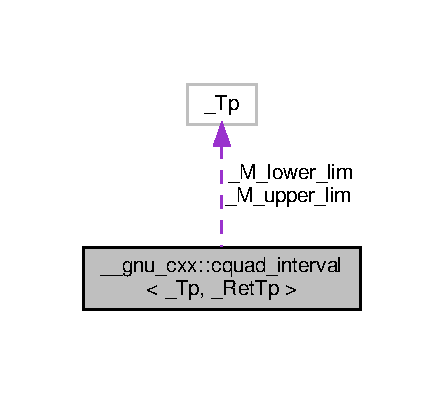
\includegraphics[width=213pt]{struct____gnu__cxx_1_1cquad__interval__coll__graph}
\end{center}
\end{figure}
\subsection*{Public Types}
\begin{DoxyCompactItemize}
\item 
using \hyperlink{struct____gnu__cxx_1_1cquad__interval_a3d2a1bbd0064e2a6c6edbcd514585311}{\+\_\+\+Abs\+Area\+Tp} = decltype(std\+::abs(\hyperlink{struct____gnu__cxx_1_1cquad__interval_aceac510aa3323d55b31555f96133cb40}{\+\_\+\+Area\+Tp}\{\}))
\item 
using \hyperlink{struct____gnu__cxx_1_1cquad__interval_aceac510aa3323d55b31555f96133cb40}{\+\_\+\+Area\+Tp} = decltype(\hyperlink{namespace____gnu__cxx_a886e03ece3d53ff7fa6c098a40f93fa5}{\+\_\+\+Ret\+Tp}\{\} $\ast$\hyperlink{namespace____gnu__cxx_a3b19a9c800ca194374ef9172290f7d79}{\+\_\+\+Tp}\{\})
\end{DoxyCompactItemize}
\subsection*{Public Attributes}
\begin{DoxyCompactItemize}
\item 
\hyperlink{struct____gnu__cxx_1_1cquad__interval_a3d2a1bbd0064e2a6c6edbcd514585311}{\+\_\+\+Abs\+Area\+Tp} \hyperlink{struct____gnu__cxx_1_1cquad__interval_a63edd4bbb3614217b24256c7a3b305b8}{\+\_\+\+M\+\_\+abs\+\_\+error}
\item 
\hyperlink{namespace____gnu__cxx_a886e03ece3d53ff7fa6c098a40f93fa5}{\+\_\+\+Ret\+Tp} \hyperlink{struct____gnu__cxx_1_1cquad__interval_a852e4c25203cf39c21e0eeb16dd70bda}{\+\_\+\+M\+\_\+coeff} \mbox{[}64\mbox{]}
\item 
\hyperlink{namespace____gnu__cxx_a3b19a9c800ca194374ef9172290f7d79}{\+\_\+\+Tp} \hyperlink{struct____gnu__cxx_1_1cquad__interval_a075cfcb47735ad5b69190a2246780475}{\+\_\+\+M\+\_\+lower\+\_\+lim}
\item 
\hyperlink{struct____gnu__cxx_1_1cquad__interval_aceac510aa3323d55b31555f96133cb40}{\+\_\+\+Area\+Tp} \hyperlink{struct____gnu__cxx_1_1cquad__interval_abb2d5586cea60c80bd99051f2ba27063}{\+\_\+\+M\+\_\+result}
\item 
\hyperlink{namespace____gnu__cxx_a3b19a9c800ca194374ef9172290f7d79}{\+\_\+\+Tp} \hyperlink{struct____gnu__cxx_1_1cquad__interval_a60b4fdf494ba274bce6271fd1fa5aa69}{\+\_\+\+M\+\_\+upper\+\_\+lim}
\item 
std\+::size\+\_\+t \hyperlink{struct____gnu__cxx_1_1cquad__interval_af4a321c6e64f7de6ab0cbf4ebd4381a7}{depth}
\item 
std\+::array$<$ \hyperlink{namespace____gnu__cxx_a886e03ece3d53ff7fa6c098a40f93fa5}{\+\_\+\+Ret\+Tp}, 33 $>$ \hyperlink{struct____gnu__cxx_1_1cquad__interval_ab3c4ae7b9f1ad8fe99f385e388514fae}{fx}
\item 
std\+::size\+\_\+t \hyperlink{struct____gnu__cxx_1_1cquad__interval_a79dbc370bba05fb7449645054889d308}{ndiv}
\item 
std\+::size\+\_\+t \hyperlink{struct____gnu__cxx_1_1cquad__interval_a82e60c6a4a1c360f09829fb6480e2888}{rdepth}
\end{DoxyCompactItemize}


\subsection{Detailed Description}
\subsubsection*{template$<$typename \+\_\+\+Tp, typename \+\_\+\+Ret\+Tp$>$\newline
struct \+\_\+\+\_\+gnu\+\_\+cxx\+::cquad\+\_\+interval$<$ \+\_\+\+Tp, \+\_\+\+Ret\+Tp $>$}

Data of a single interval. 

Definition at line 38 of file cquad\+\_\+workspace.\+h.



\subsection{Member Typedef Documentation}
\mbox{\Hypertarget{struct____gnu__cxx_1_1cquad__interval_a3d2a1bbd0064e2a6c6edbcd514585311}\label{struct____gnu__cxx_1_1cquad__interval_a3d2a1bbd0064e2a6c6edbcd514585311}} 
\index{\+\_\+\+\_\+gnu\+\_\+cxx\+::cquad\+\_\+interval@{\+\_\+\+\_\+gnu\+\_\+cxx\+::cquad\+\_\+interval}!\+\_\+\+Abs\+Area\+Tp@{\+\_\+\+Abs\+Area\+Tp}}
\index{\+\_\+\+Abs\+Area\+Tp@{\+\_\+\+Abs\+Area\+Tp}!\+\_\+\+\_\+gnu\+\_\+cxx\+::cquad\+\_\+interval@{\+\_\+\+\_\+gnu\+\_\+cxx\+::cquad\+\_\+interval}}
\subsubsection{\texorpdfstring{\+\_\+\+Abs\+Area\+Tp}{\_AbsAreaTp}}
{\footnotesize\ttfamily template$<$typename \+\_\+\+Tp, typename \+\_\+\+Ret\+Tp$>$ \\
using \hyperlink{struct____gnu__cxx_1_1cquad__interval}{\+\_\+\+\_\+gnu\+\_\+cxx\+::cquad\+\_\+interval}$<$ \hyperlink{namespace____gnu__cxx_a3b19a9c800ca194374ef9172290f7d79}{\+\_\+\+Tp}, \hyperlink{namespace____gnu__cxx_a886e03ece3d53ff7fa6c098a40f93fa5}{\+\_\+\+Ret\+Tp} $>$\+::\hyperlink{struct____gnu__cxx_1_1cquad__interval_a3d2a1bbd0064e2a6c6edbcd514585311}{\+\_\+\+Abs\+Area\+Tp} =  decltype(std\+::abs(\hyperlink{struct____gnu__cxx_1_1cquad__interval_aceac510aa3323d55b31555f96133cb40}{\+\_\+\+Area\+Tp}\{\}))}



Definition at line 41 of file cquad\+\_\+workspace.\+h.

\mbox{\Hypertarget{struct____gnu__cxx_1_1cquad__interval_aceac510aa3323d55b31555f96133cb40}\label{struct____gnu__cxx_1_1cquad__interval_aceac510aa3323d55b31555f96133cb40}} 
\index{\+\_\+\+\_\+gnu\+\_\+cxx\+::cquad\+\_\+interval@{\+\_\+\+\_\+gnu\+\_\+cxx\+::cquad\+\_\+interval}!\+\_\+\+Area\+Tp@{\+\_\+\+Area\+Tp}}
\index{\+\_\+\+Area\+Tp@{\+\_\+\+Area\+Tp}!\+\_\+\+\_\+gnu\+\_\+cxx\+::cquad\+\_\+interval@{\+\_\+\+\_\+gnu\+\_\+cxx\+::cquad\+\_\+interval}}
\subsubsection{\texorpdfstring{\+\_\+\+Area\+Tp}{\_AreaTp}}
{\footnotesize\ttfamily template$<$typename \+\_\+\+Tp, typename \+\_\+\+Ret\+Tp$>$ \\
using \hyperlink{struct____gnu__cxx_1_1cquad__interval}{\+\_\+\+\_\+gnu\+\_\+cxx\+::cquad\+\_\+interval}$<$ \hyperlink{namespace____gnu__cxx_a3b19a9c800ca194374ef9172290f7d79}{\+\_\+\+Tp}, \hyperlink{namespace____gnu__cxx_a886e03ece3d53ff7fa6c098a40f93fa5}{\+\_\+\+Ret\+Tp} $>$\+::\hyperlink{struct____gnu__cxx_1_1cquad__interval_aceac510aa3323d55b31555f96133cb40}{\+\_\+\+Area\+Tp} =  decltype(\hyperlink{namespace____gnu__cxx_a886e03ece3d53ff7fa6c098a40f93fa5}{\+\_\+\+Ret\+Tp}\{\} $\ast$ \hyperlink{namespace____gnu__cxx_a3b19a9c800ca194374ef9172290f7d79}{\+\_\+\+Tp}\{\})}



Definition at line 40 of file cquad\+\_\+workspace.\+h.



\subsection{Member Data Documentation}
\mbox{\Hypertarget{struct____gnu__cxx_1_1cquad__interval_a63edd4bbb3614217b24256c7a3b305b8}\label{struct____gnu__cxx_1_1cquad__interval_a63edd4bbb3614217b24256c7a3b305b8}} 
\index{\+\_\+\+\_\+gnu\+\_\+cxx\+::cquad\+\_\+interval@{\+\_\+\+\_\+gnu\+\_\+cxx\+::cquad\+\_\+interval}!\+\_\+\+M\+\_\+abs\+\_\+error@{\+\_\+\+M\+\_\+abs\+\_\+error}}
\index{\+\_\+\+M\+\_\+abs\+\_\+error@{\+\_\+\+M\+\_\+abs\+\_\+error}!\+\_\+\+\_\+gnu\+\_\+cxx\+::cquad\+\_\+interval@{\+\_\+\+\_\+gnu\+\_\+cxx\+::cquad\+\_\+interval}}
\subsubsection{\texorpdfstring{\+\_\+\+M\+\_\+abs\+\_\+error}{\_M\_abs\_error}}
{\footnotesize\ttfamily template$<$typename \+\_\+\+Tp, typename \+\_\+\+Ret\+Tp$>$ \\
\hyperlink{struct____gnu__cxx_1_1cquad__interval_a3d2a1bbd0064e2a6c6edbcd514585311}{\+\_\+\+Abs\+Area\+Tp} \hyperlink{struct____gnu__cxx_1_1cquad__interval}{\+\_\+\+\_\+gnu\+\_\+cxx\+::cquad\+\_\+interval}$<$ \hyperlink{namespace____gnu__cxx_a3b19a9c800ca194374ef9172290f7d79}{\+\_\+\+Tp}, \hyperlink{namespace____gnu__cxx_a886e03ece3d53ff7fa6c098a40f93fa5}{\+\_\+\+Ret\+Tp} $>$\+::\+\_\+\+M\+\_\+abs\+\_\+error}



Definition at line 46 of file cquad\+\_\+workspace.\+h.



Referenced by \+\_\+\+\_\+gnu\+\_\+cxx\+::cquad\+\_\+integrate(), \+\_\+\+\_\+gnu\+\_\+cxx\+::cquad\+\_\+interval\+\_\+comp$<$ \+\_\+\+Tp, \+\_\+\+Ret\+Tp $>$\+::operator()(), and \+\_\+\+\_\+gnu\+\_\+cxx\+::operator$<$().

\mbox{\Hypertarget{struct____gnu__cxx_1_1cquad__interval_a852e4c25203cf39c21e0eeb16dd70bda}\label{struct____gnu__cxx_1_1cquad__interval_a852e4c25203cf39c21e0eeb16dd70bda}} 
\index{\+\_\+\+\_\+gnu\+\_\+cxx\+::cquad\+\_\+interval@{\+\_\+\+\_\+gnu\+\_\+cxx\+::cquad\+\_\+interval}!\+\_\+\+M\+\_\+coeff@{\+\_\+\+M\+\_\+coeff}}
\index{\+\_\+\+M\+\_\+coeff@{\+\_\+\+M\+\_\+coeff}!\+\_\+\+\_\+gnu\+\_\+cxx\+::cquad\+\_\+interval@{\+\_\+\+\_\+gnu\+\_\+cxx\+::cquad\+\_\+interval}}
\subsubsection{\texorpdfstring{\+\_\+\+M\+\_\+coeff}{\_M\_coeff}}
{\footnotesize\ttfamily template$<$typename \+\_\+\+Tp, typename \+\_\+\+Ret\+Tp$>$ \\
\hyperlink{namespace____gnu__cxx_a886e03ece3d53ff7fa6c098a40f93fa5}{\+\_\+\+Ret\+Tp} \hyperlink{struct____gnu__cxx_1_1cquad__interval}{\+\_\+\+\_\+gnu\+\_\+cxx\+::cquad\+\_\+interval}$<$ \hyperlink{namespace____gnu__cxx_a3b19a9c800ca194374ef9172290f7d79}{\+\_\+\+Tp}, \hyperlink{namespace____gnu__cxx_a886e03ece3d53ff7fa6c098a40f93fa5}{\+\_\+\+Ret\+Tp} $>$\+::\+\_\+\+M\+\_\+coeff\mbox{[}64\mbox{]}}



Definition at line 47 of file cquad\+\_\+workspace.\+h.



Referenced by \+\_\+\+\_\+gnu\+\_\+cxx\+::cquad\+\_\+integrate().

\mbox{\Hypertarget{struct____gnu__cxx_1_1cquad__interval_a075cfcb47735ad5b69190a2246780475}\label{struct____gnu__cxx_1_1cquad__interval_a075cfcb47735ad5b69190a2246780475}} 
\index{\+\_\+\+\_\+gnu\+\_\+cxx\+::cquad\+\_\+interval@{\+\_\+\+\_\+gnu\+\_\+cxx\+::cquad\+\_\+interval}!\+\_\+\+M\+\_\+lower\+\_\+lim@{\+\_\+\+M\+\_\+lower\+\_\+lim}}
\index{\+\_\+\+M\+\_\+lower\+\_\+lim@{\+\_\+\+M\+\_\+lower\+\_\+lim}!\+\_\+\+\_\+gnu\+\_\+cxx\+::cquad\+\_\+interval@{\+\_\+\+\_\+gnu\+\_\+cxx\+::cquad\+\_\+interval}}
\subsubsection{\texorpdfstring{\+\_\+\+M\+\_\+lower\+\_\+lim}{\_M\_lower\_lim}}
{\footnotesize\ttfamily template$<$typename \+\_\+\+Tp, typename \+\_\+\+Ret\+Tp$>$ \\
\hyperlink{namespace____gnu__cxx_a3b19a9c800ca194374ef9172290f7d79}{\+\_\+\+Tp} \hyperlink{struct____gnu__cxx_1_1cquad__interval}{\+\_\+\+\_\+gnu\+\_\+cxx\+::cquad\+\_\+interval}$<$ \hyperlink{namespace____gnu__cxx_a3b19a9c800ca194374ef9172290f7d79}{\+\_\+\+Tp}, \hyperlink{namespace____gnu__cxx_a886e03ece3d53ff7fa6c098a40f93fa5}{\+\_\+\+Ret\+Tp} $>$\+::\+\_\+\+M\+\_\+lower\+\_\+lim}



Definition at line 43 of file cquad\+\_\+workspace.\+h.



Referenced by \+\_\+\+\_\+gnu\+\_\+cxx\+::cquad\+\_\+integrate().

\mbox{\Hypertarget{struct____gnu__cxx_1_1cquad__interval_abb2d5586cea60c80bd99051f2ba27063}\label{struct____gnu__cxx_1_1cquad__interval_abb2d5586cea60c80bd99051f2ba27063}} 
\index{\+\_\+\+\_\+gnu\+\_\+cxx\+::cquad\+\_\+interval@{\+\_\+\+\_\+gnu\+\_\+cxx\+::cquad\+\_\+interval}!\+\_\+\+M\+\_\+result@{\+\_\+\+M\+\_\+result}}
\index{\+\_\+\+M\+\_\+result@{\+\_\+\+M\+\_\+result}!\+\_\+\+\_\+gnu\+\_\+cxx\+::cquad\+\_\+interval@{\+\_\+\+\_\+gnu\+\_\+cxx\+::cquad\+\_\+interval}}
\subsubsection{\texorpdfstring{\+\_\+\+M\+\_\+result}{\_M\_result}}
{\footnotesize\ttfamily template$<$typename \+\_\+\+Tp, typename \+\_\+\+Ret\+Tp$>$ \\
\hyperlink{struct____gnu__cxx_1_1cquad__interval_aceac510aa3323d55b31555f96133cb40}{\+\_\+\+Area\+Tp} \hyperlink{struct____gnu__cxx_1_1cquad__interval}{\+\_\+\+\_\+gnu\+\_\+cxx\+::cquad\+\_\+interval}$<$ \hyperlink{namespace____gnu__cxx_a3b19a9c800ca194374ef9172290f7d79}{\+\_\+\+Tp}, \hyperlink{namespace____gnu__cxx_a886e03ece3d53ff7fa6c098a40f93fa5}{\+\_\+\+Ret\+Tp} $>$\+::\+\_\+\+M\+\_\+result}



Definition at line 45 of file cquad\+\_\+workspace.\+h.



Referenced by \+\_\+\+\_\+gnu\+\_\+cxx\+::cquad\+\_\+integrate().

\mbox{\Hypertarget{struct____gnu__cxx_1_1cquad__interval_a60b4fdf494ba274bce6271fd1fa5aa69}\label{struct____gnu__cxx_1_1cquad__interval_a60b4fdf494ba274bce6271fd1fa5aa69}} 
\index{\+\_\+\+\_\+gnu\+\_\+cxx\+::cquad\+\_\+interval@{\+\_\+\+\_\+gnu\+\_\+cxx\+::cquad\+\_\+interval}!\+\_\+\+M\+\_\+upper\+\_\+lim@{\+\_\+\+M\+\_\+upper\+\_\+lim}}
\index{\+\_\+\+M\+\_\+upper\+\_\+lim@{\+\_\+\+M\+\_\+upper\+\_\+lim}!\+\_\+\+\_\+gnu\+\_\+cxx\+::cquad\+\_\+interval@{\+\_\+\+\_\+gnu\+\_\+cxx\+::cquad\+\_\+interval}}
\subsubsection{\texorpdfstring{\+\_\+\+M\+\_\+upper\+\_\+lim}{\_M\_upper\_lim}}
{\footnotesize\ttfamily template$<$typename \+\_\+\+Tp, typename \+\_\+\+Ret\+Tp$>$ \\
\hyperlink{namespace____gnu__cxx_a3b19a9c800ca194374ef9172290f7d79}{\+\_\+\+Tp} \hyperlink{struct____gnu__cxx_1_1cquad__interval}{\+\_\+\+\_\+gnu\+\_\+cxx\+::cquad\+\_\+interval}$<$ \hyperlink{namespace____gnu__cxx_a3b19a9c800ca194374ef9172290f7d79}{\+\_\+\+Tp}, \hyperlink{namespace____gnu__cxx_a886e03ece3d53ff7fa6c098a40f93fa5}{\+\_\+\+Ret\+Tp} $>$\+::\+\_\+\+M\+\_\+upper\+\_\+lim}



Definition at line 44 of file cquad\+\_\+workspace.\+h.



Referenced by \+\_\+\+\_\+gnu\+\_\+cxx\+::cquad\+\_\+integrate().

\mbox{\Hypertarget{struct____gnu__cxx_1_1cquad__interval_af4a321c6e64f7de6ab0cbf4ebd4381a7}\label{struct____gnu__cxx_1_1cquad__interval_af4a321c6e64f7de6ab0cbf4ebd4381a7}} 
\index{\+\_\+\+\_\+gnu\+\_\+cxx\+::cquad\+\_\+interval@{\+\_\+\+\_\+gnu\+\_\+cxx\+::cquad\+\_\+interval}!depth@{depth}}
\index{depth@{depth}!\+\_\+\+\_\+gnu\+\_\+cxx\+::cquad\+\_\+interval@{\+\_\+\+\_\+gnu\+\_\+cxx\+::cquad\+\_\+interval}}
\subsubsection{\texorpdfstring{depth}{depth}}
{\footnotesize\ttfamily template$<$typename \+\_\+\+Tp, typename \+\_\+\+Ret\+Tp$>$ \\
std\+::size\+\_\+t \hyperlink{struct____gnu__cxx_1_1cquad__interval}{\+\_\+\+\_\+gnu\+\_\+cxx\+::cquad\+\_\+interval}$<$ \hyperlink{namespace____gnu__cxx_a3b19a9c800ca194374ef9172290f7d79}{\+\_\+\+Tp}, \hyperlink{namespace____gnu__cxx_a886e03ece3d53ff7fa6c098a40f93fa5}{\+\_\+\+Ret\+Tp} $>$\+::depth}



Definition at line 49 of file cquad\+\_\+workspace.\+h.



Referenced by \+\_\+\+\_\+gnu\+\_\+cxx\+::cquad\+\_\+integrate().

\mbox{\Hypertarget{struct____gnu__cxx_1_1cquad__interval_ab3c4ae7b9f1ad8fe99f385e388514fae}\label{struct____gnu__cxx_1_1cquad__interval_ab3c4ae7b9f1ad8fe99f385e388514fae}} 
\index{\+\_\+\+\_\+gnu\+\_\+cxx\+::cquad\+\_\+interval@{\+\_\+\+\_\+gnu\+\_\+cxx\+::cquad\+\_\+interval}!fx@{fx}}
\index{fx@{fx}!\+\_\+\+\_\+gnu\+\_\+cxx\+::cquad\+\_\+interval@{\+\_\+\+\_\+gnu\+\_\+cxx\+::cquad\+\_\+interval}}
\subsubsection{\texorpdfstring{fx}{fx}}
{\footnotesize\ttfamily template$<$typename \+\_\+\+Tp, typename \+\_\+\+Ret\+Tp$>$ \\
std\+::array$<$\hyperlink{namespace____gnu__cxx_a886e03ece3d53ff7fa6c098a40f93fa5}{\+\_\+\+Ret\+Tp}, 33$>$ \hyperlink{struct____gnu__cxx_1_1cquad__interval}{\+\_\+\+\_\+gnu\+\_\+cxx\+::cquad\+\_\+interval}$<$ \hyperlink{namespace____gnu__cxx_a3b19a9c800ca194374ef9172290f7d79}{\+\_\+\+Tp}, \hyperlink{namespace____gnu__cxx_a886e03ece3d53ff7fa6c098a40f93fa5}{\+\_\+\+Ret\+Tp} $>$\+::fx}



Definition at line 48 of file cquad\+\_\+workspace.\+h.



Referenced by \+\_\+\+\_\+gnu\+\_\+cxx\+::cquad\+\_\+integrate().

\mbox{\Hypertarget{struct____gnu__cxx_1_1cquad__interval_a79dbc370bba05fb7449645054889d308}\label{struct____gnu__cxx_1_1cquad__interval_a79dbc370bba05fb7449645054889d308}} 
\index{\+\_\+\+\_\+gnu\+\_\+cxx\+::cquad\+\_\+interval@{\+\_\+\+\_\+gnu\+\_\+cxx\+::cquad\+\_\+interval}!ndiv@{ndiv}}
\index{ndiv@{ndiv}!\+\_\+\+\_\+gnu\+\_\+cxx\+::cquad\+\_\+interval@{\+\_\+\+\_\+gnu\+\_\+cxx\+::cquad\+\_\+interval}}
\subsubsection{\texorpdfstring{ndiv}{ndiv}}
{\footnotesize\ttfamily template$<$typename \+\_\+\+Tp, typename \+\_\+\+Ret\+Tp$>$ \\
std\+::size\+\_\+t \hyperlink{struct____gnu__cxx_1_1cquad__interval}{\+\_\+\+\_\+gnu\+\_\+cxx\+::cquad\+\_\+interval}$<$ \hyperlink{namespace____gnu__cxx_a3b19a9c800ca194374ef9172290f7d79}{\+\_\+\+Tp}, \hyperlink{namespace____gnu__cxx_a886e03ece3d53ff7fa6c098a40f93fa5}{\+\_\+\+Ret\+Tp} $>$\+::ndiv}



Definition at line 51 of file cquad\+\_\+workspace.\+h.



Referenced by \+\_\+\+\_\+gnu\+\_\+cxx\+::cquad\+\_\+integrate().

\mbox{\Hypertarget{struct____gnu__cxx_1_1cquad__interval_a82e60c6a4a1c360f09829fb6480e2888}\label{struct____gnu__cxx_1_1cquad__interval_a82e60c6a4a1c360f09829fb6480e2888}} 
\index{\+\_\+\+\_\+gnu\+\_\+cxx\+::cquad\+\_\+interval@{\+\_\+\+\_\+gnu\+\_\+cxx\+::cquad\+\_\+interval}!rdepth@{rdepth}}
\index{rdepth@{rdepth}!\+\_\+\+\_\+gnu\+\_\+cxx\+::cquad\+\_\+interval@{\+\_\+\+\_\+gnu\+\_\+cxx\+::cquad\+\_\+interval}}
\subsubsection{\texorpdfstring{rdepth}{rdepth}}
{\footnotesize\ttfamily template$<$typename \+\_\+\+Tp, typename \+\_\+\+Ret\+Tp$>$ \\
std\+::size\+\_\+t \hyperlink{struct____gnu__cxx_1_1cquad__interval}{\+\_\+\+\_\+gnu\+\_\+cxx\+::cquad\+\_\+interval}$<$ \hyperlink{namespace____gnu__cxx_a3b19a9c800ca194374ef9172290f7d79}{\+\_\+\+Tp}, \hyperlink{namespace____gnu__cxx_a886e03ece3d53ff7fa6c098a40f93fa5}{\+\_\+\+Ret\+Tp} $>$\+::rdepth}



Definition at line 50 of file cquad\+\_\+workspace.\+h.



Referenced by \+\_\+\+\_\+gnu\+\_\+cxx\+::cquad\+\_\+integrate().



The documentation for this struct was generated from the following file\+:\begin{DoxyCompactItemize}
\item 
include/ext/\hyperlink{cquad__workspace_8h}{cquad\+\_\+workspace.\+h}\end{DoxyCompactItemize}

\hypertarget{struct____gnu__cxx_1_1cquad__interval__comp}{}\section{\+\_\+\+\_\+gnu\+\_\+cxx\+:\+:cquad\+\_\+interval\+\_\+comp$<$ \+\_\+\+Tp, \+\_\+\+Ret\+Tp $>$ Struct Template Reference}
\label{struct____gnu__cxx_1_1cquad__interval__comp}\index{\+\_\+\+\_\+gnu\+\_\+cxx\+::cquad\+\_\+interval\+\_\+comp$<$ \+\_\+\+Tp, \+\_\+\+Ret\+Tp $>$@{\+\_\+\+\_\+gnu\+\_\+cxx\+::cquad\+\_\+interval\+\_\+comp$<$ \+\_\+\+Tp, \+\_\+\+Ret\+Tp $>$}}


{\ttfamily \#include $<$cquad\+\_\+workspace.\+h$>$}

\subsection*{Public Member Functions}
\begin{DoxyCompactItemize}
\item 
\hyperlink{namespace____gnu__cxx_ae83aca57f97767d5d09188718728a0ac}{bool} \hyperlink{struct____gnu__cxx_1_1cquad__interval__comp_ac0a0d43bec114cb4d09639ae6b21085d}{operator()} (const \hyperlink{struct____gnu__cxx_1_1cquad__interval}{cquad\+\_\+interval}$<$ \hyperlink{namespace____gnu__cxx_a3b19a9c800ca194374ef9172290f7d79}{\+\_\+\+Tp}, \hyperlink{namespace____gnu__cxx_a886e03ece3d53ff7fa6c098a40f93fa5}{\+\_\+\+Ret\+Tp} $>$ \&\+\_\+\+\_\+ivl, const \hyperlink{struct____gnu__cxx_1_1cquad__interval}{cquad\+\_\+interval}$<$ \hyperlink{namespace____gnu__cxx_a3b19a9c800ca194374ef9172290f7d79}{\+\_\+\+Tp}, \hyperlink{namespace____gnu__cxx_a886e03ece3d53ff7fa6c098a40f93fa5}{\+\_\+\+Ret\+Tp} $>$ \&\+\_\+\+\_\+ivr)
\end{DoxyCompactItemize}


\subsection{Detailed Description}
\subsubsection*{template$<$typename \+\_\+\+Tp, typename \+\_\+\+Ret\+Tp$>$\newline
struct \+\_\+\+\_\+gnu\+\_\+cxx\+::cquad\+\_\+interval\+\_\+comp$<$ \+\_\+\+Tp, \+\_\+\+Ret\+Tp $>$}



Definition at line 64 of file cquad\+\_\+workspace.\+h.



\subsection{Member Function Documentation}
\mbox{\Hypertarget{struct____gnu__cxx_1_1cquad__interval__comp_ac0a0d43bec114cb4d09639ae6b21085d}\label{struct____gnu__cxx_1_1cquad__interval__comp_ac0a0d43bec114cb4d09639ae6b21085d}} 
\index{\+\_\+\+\_\+gnu\+\_\+cxx\+::cquad\+\_\+interval\+\_\+comp@{\+\_\+\+\_\+gnu\+\_\+cxx\+::cquad\+\_\+interval\+\_\+comp}!operator()@{operator()}}
\index{operator()@{operator()}!\+\_\+\+\_\+gnu\+\_\+cxx\+::cquad\+\_\+interval\+\_\+comp@{\+\_\+\+\_\+gnu\+\_\+cxx\+::cquad\+\_\+interval\+\_\+comp}}
\subsubsection{\texorpdfstring{operator()()}{operator()()}}
{\footnotesize\ttfamily template$<$typename \+\_\+\+Tp , typename \+\_\+\+Ret\+Tp $>$ \\
\hyperlink{namespace____gnu__cxx_ae83aca57f97767d5d09188718728a0ac}{bool} \hyperlink{struct____gnu__cxx_1_1cquad__interval__comp}{\+\_\+\+\_\+gnu\+\_\+cxx\+::cquad\+\_\+interval\+\_\+comp}$<$ \hyperlink{namespace____gnu__cxx_a3b19a9c800ca194374ef9172290f7d79}{\+\_\+\+Tp}, \hyperlink{namespace____gnu__cxx_a886e03ece3d53ff7fa6c098a40f93fa5}{\+\_\+\+Ret\+Tp} $>$\+::operator() (\begin{DoxyParamCaption}\item[{const \hyperlink{struct____gnu__cxx_1_1cquad__interval}{cquad\+\_\+interval}$<$ \hyperlink{namespace____gnu__cxx_a3b19a9c800ca194374ef9172290f7d79}{\+\_\+\+Tp}, \hyperlink{namespace____gnu__cxx_a886e03ece3d53ff7fa6c098a40f93fa5}{\+\_\+\+Ret\+Tp} $>$ \&}]{\+\_\+\+\_\+ivl,  }\item[{const \hyperlink{struct____gnu__cxx_1_1cquad__interval}{cquad\+\_\+interval}$<$ \hyperlink{namespace____gnu__cxx_a3b19a9c800ca194374ef9172290f7d79}{\+\_\+\+Tp}, \hyperlink{namespace____gnu__cxx_a886e03ece3d53ff7fa6c098a40f93fa5}{\+\_\+\+Ret\+Tp} $>$ \&}]{\+\_\+\+\_\+ivr }\end{DoxyParamCaption})\hspace{0.3cm}{\ttfamily [inline]}}



Definition at line 67 of file cquad\+\_\+workspace.\+h.



References \+\_\+\+\_\+gnu\+\_\+cxx\+::cquad\+\_\+interval$<$ \+\_\+\+Tp, \+\_\+\+Ret\+Tp $>$\+::\+\_\+\+M\+\_\+abs\+\_\+error.


\begin{DoxyCode}
69       \{ \textcolor{keywordflow}{return} \_\_ivl.\_M\_abs\_error < \_\_ivr.\_M\_abs\_error; \}
\end{DoxyCode}


The documentation for this struct was generated from the following file\+:\begin{DoxyCompactItemize}
\item 
include/ext/\hyperlink{cquad__workspace_8h}{cquad\+\_\+workspace.\+h}\end{DoxyCompactItemize}

\hypertarget{struct____gnu__cxx_1_1cquad__workspace}{}\section{\+\_\+\+\_\+gnu\+\_\+cxx\+:\+:cquad\+\_\+workspace$<$ \+\_\+\+Tp, \+\_\+\+Ret\+Tp $>$ Struct Template Reference}
\label{struct____gnu__cxx_1_1cquad__workspace}\index{\+\_\+\+\_\+gnu\+\_\+cxx\+::cquad\+\_\+workspace$<$ \+\_\+\+Tp, \+\_\+\+Ret\+Tp $>$@{\+\_\+\+\_\+gnu\+\_\+cxx\+::cquad\+\_\+workspace$<$ \+\_\+\+Tp, \+\_\+\+Ret\+Tp $>$}}


{\ttfamily \#include $<$cquad\+\_\+workspace.\+h$>$}

\subsection*{Public Types}
\begin{DoxyCompactItemize}
\item 
using \hyperlink{struct____gnu__cxx_1_1cquad__workspace_a7abfe6354869dc61f6109c9e807ec152}{\+\_\+\+Abs\+Area\+Tp} = decltype(std\+::abs(\hyperlink{struct____gnu__cxx_1_1cquad__workspace_a8eede64f10ac7bbf817992cd3d06fa8f}{\+\_\+\+Area\+Tp}\{\}))
\item 
using \hyperlink{struct____gnu__cxx_1_1cquad__workspace_a8eede64f10ac7bbf817992cd3d06fa8f}{\+\_\+\+Area\+Tp} = decltype(\hyperlink{namespace____gnu__cxx_a886e03ece3d53ff7fa6c098a40f93fa5}{\+\_\+\+Ret\+Tp}\{\} $\ast$\hyperlink{namespace____gnu__cxx_a3b19a9c800ca194374ef9172290f7d79}{\+\_\+\+Tp}\{\})
\end{DoxyCompactItemize}
\subsection*{Public Member Functions}
\begin{DoxyCompactItemize}
\item 
\hyperlink{struct____gnu__cxx_1_1cquad__workspace_a3d7601160fd8f630b70109b61f493738}{cquad\+\_\+workspace} (std\+::size\+\_\+t \+\_\+\+\_\+len=200)
\item 
std\+::vector$<$ \hyperlink{struct____gnu__cxx_1_1cquad__interval}{cquad\+\_\+interval}$<$ \hyperlink{namespace____gnu__cxx_a3b19a9c800ca194374ef9172290f7d79}{\+\_\+\+Tp}, \hyperlink{namespace____gnu__cxx_a886e03ece3d53ff7fa6c098a40f93fa5}{\+\_\+\+Ret\+Tp} $>$ $>$\+::iterator \hyperlink{struct____gnu__cxx_1_1cquad__workspace_adf18a306dbf58cb00b4c6254266816bc}{begin} ()
\item 
std\+::size\+\_\+t \hyperlink{struct____gnu__cxx_1_1cquad__workspace_a379ef600e71c787579e107ffef46fcdf}{capacity} () const
\item 
void \hyperlink{struct____gnu__cxx_1_1cquad__workspace_ac3b3e8c4e17571349b56ac1635789b34}{clear} ()
\item 
std\+::vector$<$ \hyperlink{struct____gnu__cxx_1_1cquad__interval}{cquad\+\_\+interval}$<$ \hyperlink{namespace____gnu__cxx_a3b19a9c800ca194374ef9172290f7d79}{\+\_\+\+Tp}, \hyperlink{namespace____gnu__cxx_a886e03ece3d53ff7fa6c098a40f93fa5}{\+\_\+\+Ret\+Tp} $>$ $>$\+::iterator \hyperlink{struct____gnu__cxx_1_1cquad__workspace_a61729a1acaa035013ebb0ed6e4ffcbf4}{end} ()
\item 
void \hyperlink{struct____gnu__cxx_1_1cquad__workspace_a34cca20d45326741147cf0397a63a9e9}{pop} ()
\item 
void \hyperlink{struct____gnu__cxx_1_1cquad__workspace_ab8b17ed5aea295adbf9a70b84498c948}{push} (const \hyperlink{struct____gnu__cxx_1_1cquad__interval}{cquad\+\_\+interval}$<$ \hyperlink{namespace____gnu__cxx_a3b19a9c800ca194374ef9172290f7d79}{\+\_\+\+Tp}, \hyperlink{namespace____gnu__cxx_a886e03ece3d53ff7fa6c098a40f93fa5}{\+\_\+\+Ret\+Tp} $>$ \&\+\_\+\+\_\+iv)
\item 
std\+::size\+\_\+t \hyperlink{struct____gnu__cxx_1_1cquad__workspace_aafe82f4041e233329f4510ca34a9e619}{size} () const
\item 
const \hyperlink{struct____gnu__cxx_1_1cquad__interval}{cquad\+\_\+interval}$<$ \hyperlink{namespace____gnu__cxx_a3b19a9c800ca194374ef9172290f7d79}{\+\_\+\+Tp}, \hyperlink{namespace____gnu__cxx_a886e03ece3d53ff7fa6c098a40f93fa5}{\+\_\+\+Ret\+Tp} $>$ \& \hyperlink{struct____gnu__cxx_1_1cquad__workspace_a6da1e7fd72a9a94fba84699b4f10a3b6}{top} () const
\item 
\hyperlink{struct____gnu__cxx_1_1cquad__interval}{cquad\+\_\+interval}$<$ \hyperlink{namespace____gnu__cxx_a3b19a9c800ca194374ef9172290f7d79}{\+\_\+\+Tp}, \hyperlink{namespace____gnu__cxx_a886e03ece3d53ff7fa6c098a40f93fa5}{\+\_\+\+Ret\+Tp} $>$ \& \hyperlink{struct____gnu__cxx_1_1cquad__workspace_a6045595044796357d25adb9a12119b30}{top} ()
\item 
\hyperlink{struct____gnu__cxx_1_1cquad__workspace_a7abfe6354869dc61f6109c9e807ec152}{\+\_\+\+Abs\+Area\+Tp} \hyperlink{struct____gnu__cxx_1_1cquad__workspace_a9eb68447dc880ef6de7cd695d7e223ae}{total\+\_\+error} () const
\item 
\hyperlink{struct____gnu__cxx_1_1cquad__workspace_a8eede64f10ac7bbf817992cd3d06fa8f}{\+\_\+\+Area\+Tp} \hyperlink{struct____gnu__cxx_1_1cquad__workspace_aa429f45aacd05932104d5f91e6a0ff43}{total\+\_\+integral} () const
\item 
void \hyperlink{struct____gnu__cxx_1_1cquad__workspace_a40032babd2a04f33cd7c37d9c80d1d50}{update} ()
\end{DoxyCompactItemize}
\subsection*{Public Attributes}
\begin{DoxyCompactItemize}
\item 
std\+::vector$<$ \hyperlink{struct____gnu__cxx_1_1cquad__interval}{cquad\+\_\+interval}$<$ \hyperlink{namespace____gnu__cxx_a3b19a9c800ca194374ef9172290f7d79}{\+\_\+\+Tp}, \hyperlink{namespace____gnu__cxx_a886e03ece3d53ff7fa6c098a40f93fa5}{\+\_\+\+Ret\+Tp} $>$ $>$ \hyperlink{struct____gnu__cxx_1_1cquad__workspace_a46edeb05c52f2a406dc582b404fe83e6}{\+\_\+\+M\+\_\+ival}
\end{DoxyCompactItemize}


\subsection{Detailed Description}
\subsubsection*{template$<$typename \+\_\+\+Tp, typename \+\_\+\+Ret\+Tp$>$\newline
struct \+\_\+\+\_\+gnu\+\_\+cxx\+::cquad\+\_\+workspace$<$ \+\_\+\+Tp, \+\_\+\+Ret\+Tp $>$}

The workspace is a collection of intervals. Actually, it is a priority queue where the priority is the absolute error of the interval integral. 

Definition at line 78 of file cquad\+\_\+workspace.\+h.



\subsection{Member Typedef Documentation}
\mbox{\Hypertarget{struct____gnu__cxx_1_1cquad__workspace_a7abfe6354869dc61f6109c9e807ec152}\label{struct____gnu__cxx_1_1cquad__workspace_a7abfe6354869dc61f6109c9e807ec152}} 
\index{\+\_\+\+\_\+gnu\+\_\+cxx\+::cquad\+\_\+workspace@{\+\_\+\+\_\+gnu\+\_\+cxx\+::cquad\+\_\+workspace}!\+\_\+\+Abs\+Area\+Tp@{\+\_\+\+Abs\+Area\+Tp}}
\index{\+\_\+\+Abs\+Area\+Tp@{\+\_\+\+Abs\+Area\+Tp}!\+\_\+\+\_\+gnu\+\_\+cxx\+::cquad\+\_\+workspace@{\+\_\+\+\_\+gnu\+\_\+cxx\+::cquad\+\_\+workspace}}
\subsubsection{\texorpdfstring{\+\_\+\+Abs\+Area\+Tp}{\_AbsAreaTp}}
{\footnotesize\ttfamily template$<$typename \+\_\+\+Tp , typename \+\_\+\+Ret\+Tp $>$ \\
using \hyperlink{struct____gnu__cxx_1_1cquad__workspace}{\+\_\+\+\_\+gnu\+\_\+cxx\+::cquad\+\_\+workspace}$<$ \hyperlink{namespace____gnu__cxx_a3b19a9c800ca194374ef9172290f7d79}{\+\_\+\+Tp}, \hyperlink{namespace____gnu__cxx_a886e03ece3d53ff7fa6c098a40f93fa5}{\+\_\+\+Ret\+Tp} $>$\+::\hyperlink{struct____gnu__cxx_1_1cquad__workspace_a7abfe6354869dc61f6109c9e807ec152}{\+\_\+\+Abs\+Area\+Tp} =  decltype(std\+::abs(\hyperlink{struct____gnu__cxx_1_1cquad__workspace_a8eede64f10ac7bbf817992cd3d06fa8f}{\+\_\+\+Area\+Tp}\{\}))}



Definition at line 81 of file cquad\+\_\+workspace.\+h.

\mbox{\Hypertarget{struct____gnu__cxx_1_1cquad__workspace_a8eede64f10ac7bbf817992cd3d06fa8f}\label{struct____gnu__cxx_1_1cquad__workspace_a8eede64f10ac7bbf817992cd3d06fa8f}} 
\index{\+\_\+\+\_\+gnu\+\_\+cxx\+::cquad\+\_\+workspace@{\+\_\+\+\_\+gnu\+\_\+cxx\+::cquad\+\_\+workspace}!\+\_\+\+Area\+Tp@{\+\_\+\+Area\+Tp}}
\index{\+\_\+\+Area\+Tp@{\+\_\+\+Area\+Tp}!\+\_\+\+\_\+gnu\+\_\+cxx\+::cquad\+\_\+workspace@{\+\_\+\+\_\+gnu\+\_\+cxx\+::cquad\+\_\+workspace}}
\subsubsection{\texorpdfstring{\+\_\+\+Area\+Tp}{\_AreaTp}}
{\footnotesize\ttfamily template$<$typename \+\_\+\+Tp , typename \+\_\+\+Ret\+Tp $>$ \\
using \hyperlink{struct____gnu__cxx_1_1cquad__workspace}{\+\_\+\+\_\+gnu\+\_\+cxx\+::cquad\+\_\+workspace}$<$ \hyperlink{namespace____gnu__cxx_a3b19a9c800ca194374ef9172290f7d79}{\+\_\+\+Tp}, \hyperlink{namespace____gnu__cxx_a886e03ece3d53ff7fa6c098a40f93fa5}{\+\_\+\+Ret\+Tp} $>$\+::\hyperlink{struct____gnu__cxx_1_1cquad__workspace_a8eede64f10ac7bbf817992cd3d06fa8f}{\+\_\+\+Area\+Tp} =  decltype(\hyperlink{namespace____gnu__cxx_a886e03ece3d53ff7fa6c098a40f93fa5}{\+\_\+\+Ret\+Tp}\{\} $\ast$ \hyperlink{namespace____gnu__cxx_a3b19a9c800ca194374ef9172290f7d79}{\+\_\+\+Tp}\{\})}



Definition at line 80 of file cquad\+\_\+workspace.\+h.



\subsection{Constructor \& Destructor Documentation}
\mbox{\Hypertarget{struct____gnu__cxx_1_1cquad__workspace_a3d7601160fd8f630b70109b61f493738}\label{struct____gnu__cxx_1_1cquad__workspace_a3d7601160fd8f630b70109b61f493738}} 
\index{\+\_\+\+\_\+gnu\+\_\+cxx\+::cquad\+\_\+workspace@{\+\_\+\+\_\+gnu\+\_\+cxx\+::cquad\+\_\+workspace}!cquad\+\_\+workspace@{cquad\+\_\+workspace}}
\index{cquad\+\_\+workspace@{cquad\+\_\+workspace}!\+\_\+\+\_\+gnu\+\_\+cxx\+::cquad\+\_\+workspace@{\+\_\+\+\_\+gnu\+\_\+cxx\+::cquad\+\_\+workspace}}
\subsubsection{\texorpdfstring{cquad\+\_\+workspace()}{cquad\_workspace()}}
{\footnotesize\ttfamily template$<$typename \+\_\+\+Tp , typename \+\_\+\+Ret\+Tp $>$ \\
\hyperlink{struct____gnu__cxx_1_1cquad__workspace}{\+\_\+\+\_\+gnu\+\_\+cxx\+::cquad\+\_\+workspace}$<$ \hyperlink{namespace____gnu__cxx_a3b19a9c800ca194374ef9172290f7d79}{\+\_\+\+Tp}, \hyperlink{namespace____gnu__cxx_a886e03ece3d53ff7fa6c098a40f93fa5}{\+\_\+\+Ret\+Tp} $>$\+::\hyperlink{struct____gnu__cxx_1_1cquad__workspace}{cquad\+\_\+workspace} (\begin{DoxyParamCaption}\item[{std\+::size\+\_\+t}]{\+\_\+\+\_\+len = {\ttfamily 200} }\end{DoxyParamCaption})\hspace{0.3cm}{\ttfamily [inline]}}



Definition at line 85 of file cquad\+\_\+workspace.\+h.


\begin{DoxyCode}
86       : \hyperlink{struct____gnu__cxx_1_1cquad__workspace_a46edeb05c52f2a406dc582b404fe83e6}{\_M\_ival}()
87       \{ this->\hyperlink{struct____gnu__cxx_1_1cquad__workspace_a46edeb05c52f2a406dc582b404fe83e6}{\_M\_ival}.reserve(\_\_len); \}
\end{DoxyCode}


\subsection{Member Function Documentation}
\mbox{\Hypertarget{struct____gnu__cxx_1_1cquad__workspace_adf18a306dbf58cb00b4c6254266816bc}\label{struct____gnu__cxx_1_1cquad__workspace_adf18a306dbf58cb00b4c6254266816bc}} 
\index{\+\_\+\+\_\+gnu\+\_\+cxx\+::cquad\+\_\+workspace@{\+\_\+\+\_\+gnu\+\_\+cxx\+::cquad\+\_\+workspace}!begin@{begin}}
\index{begin@{begin}!\+\_\+\+\_\+gnu\+\_\+cxx\+::cquad\+\_\+workspace@{\+\_\+\+\_\+gnu\+\_\+cxx\+::cquad\+\_\+workspace}}
\subsubsection{\texorpdfstring{begin()}{begin()}}
{\footnotesize\ttfamily template$<$typename \+\_\+\+Tp , typename \+\_\+\+Ret\+Tp $>$ \\
std\+::vector$<$\hyperlink{struct____gnu__cxx_1_1cquad__interval}{cquad\+\_\+interval}$<$\hyperlink{namespace____gnu__cxx_a3b19a9c800ca194374ef9172290f7d79}{\+\_\+\+Tp}, \hyperlink{namespace____gnu__cxx_a886e03ece3d53ff7fa6c098a40f93fa5}{\+\_\+\+Ret\+Tp}$>$ $>$\+::iterator \hyperlink{struct____gnu__cxx_1_1cquad__workspace}{\+\_\+\+\_\+gnu\+\_\+cxx\+::cquad\+\_\+workspace}$<$ \hyperlink{namespace____gnu__cxx_a3b19a9c800ca194374ef9172290f7d79}{\+\_\+\+Tp}, \hyperlink{namespace____gnu__cxx_a886e03ece3d53ff7fa6c098a40f93fa5}{\+\_\+\+Ret\+Tp} $>$\+::begin (\begin{DoxyParamCaption}{ }\end{DoxyParamCaption})\hspace{0.3cm}{\ttfamily [inline]}}



Definition at line 97 of file cquad\+\_\+workspace.\+h.


\begin{DoxyCode}
98       \{ \textcolor{keywordflow}{return} this->\hyperlink{struct____gnu__cxx_1_1cquad__workspace_a46edeb05c52f2a406dc582b404fe83e6}{\_M\_ival}.begin(); \}
\end{DoxyCode}
\mbox{\Hypertarget{struct____gnu__cxx_1_1cquad__workspace_a379ef600e71c787579e107ffef46fcdf}\label{struct____gnu__cxx_1_1cquad__workspace_a379ef600e71c787579e107ffef46fcdf}} 
\index{\+\_\+\+\_\+gnu\+\_\+cxx\+::cquad\+\_\+workspace@{\+\_\+\+\_\+gnu\+\_\+cxx\+::cquad\+\_\+workspace}!capacity@{capacity}}
\index{capacity@{capacity}!\+\_\+\+\_\+gnu\+\_\+cxx\+::cquad\+\_\+workspace@{\+\_\+\+\_\+gnu\+\_\+cxx\+::cquad\+\_\+workspace}}
\subsubsection{\texorpdfstring{capacity()}{capacity()}}
{\footnotesize\ttfamily template$<$typename \+\_\+\+Tp , typename \+\_\+\+Ret\+Tp $>$ \\
std\+::size\+\_\+t \hyperlink{struct____gnu__cxx_1_1cquad__workspace}{\+\_\+\+\_\+gnu\+\_\+cxx\+::cquad\+\_\+workspace}$<$ \hyperlink{namespace____gnu__cxx_a3b19a9c800ca194374ef9172290f7d79}{\+\_\+\+Tp}, \hyperlink{namespace____gnu__cxx_a886e03ece3d53ff7fa6c098a40f93fa5}{\+\_\+\+Ret\+Tp} $>$\+::capacity (\begin{DoxyParamCaption}{ }\end{DoxyParamCaption}) const\hspace{0.3cm}{\ttfamily [inline]}}



Definition at line 93 of file cquad\+\_\+workspace.\+h.


\begin{DoxyCode}
94       \{ \textcolor{keywordflow}{return} this->\hyperlink{struct____gnu__cxx_1_1cquad__workspace_a46edeb05c52f2a406dc582b404fe83e6}{\_M\_ival}.capacity(); \}
\end{DoxyCode}
\mbox{\Hypertarget{struct____gnu__cxx_1_1cquad__workspace_ac3b3e8c4e17571349b56ac1635789b34}\label{struct____gnu__cxx_1_1cquad__workspace_ac3b3e8c4e17571349b56ac1635789b34}} 
\index{\+\_\+\+\_\+gnu\+\_\+cxx\+::cquad\+\_\+workspace@{\+\_\+\+\_\+gnu\+\_\+cxx\+::cquad\+\_\+workspace}!clear@{clear}}
\index{clear@{clear}!\+\_\+\+\_\+gnu\+\_\+cxx\+::cquad\+\_\+workspace@{\+\_\+\+\_\+gnu\+\_\+cxx\+::cquad\+\_\+workspace}}
\subsubsection{\texorpdfstring{clear()}{clear()}}
{\footnotesize\ttfamily template$<$typename \+\_\+\+Tp , typename \+\_\+\+Ret\+Tp $>$ \\
void \hyperlink{struct____gnu__cxx_1_1cquad__workspace}{\+\_\+\+\_\+gnu\+\_\+cxx\+::cquad\+\_\+workspace}$<$ \hyperlink{namespace____gnu__cxx_a3b19a9c800ca194374ef9172290f7d79}{\+\_\+\+Tp}, \hyperlink{namespace____gnu__cxx_a886e03ece3d53ff7fa6c098a40f93fa5}{\+\_\+\+Ret\+Tp} $>$\+::clear (\begin{DoxyParamCaption}{ }\end{DoxyParamCaption})\hspace{0.3cm}{\ttfamily [inline]}}



Definition at line 113 of file cquad\+\_\+workspace.\+h.


\begin{DoxyCode}
114       \{ this->\hyperlink{struct____gnu__cxx_1_1cquad__workspace_a46edeb05c52f2a406dc582b404fe83e6}{\_M\_ival}.clear(); \}
\end{DoxyCode}
\mbox{\Hypertarget{struct____gnu__cxx_1_1cquad__workspace_a61729a1acaa035013ebb0ed6e4ffcbf4}\label{struct____gnu__cxx_1_1cquad__workspace_a61729a1acaa035013ebb0ed6e4ffcbf4}} 
\index{\+\_\+\+\_\+gnu\+\_\+cxx\+::cquad\+\_\+workspace@{\+\_\+\+\_\+gnu\+\_\+cxx\+::cquad\+\_\+workspace}!end@{end}}
\index{end@{end}!\+\_\+\+\_\+gnu\+\_\+cxx\+::cquad\+\_\+workspace@{\+\_\+\+\_\+gnu\+\_\+cxx\+::cquad\+\_\+workspace}}
\subsubsection{\texorpdfstring{end()}{end()}}
{\footnotesize\ttfamily template$<$typename \+\_\+\+Tp , typename \+\_\+\+Ret\+Tp $>$ \\
std\+::vector$<$\hyperlink{struct____gnu__cxx_1_1cquad__interval}{cquad\+\_\+interval}$<$\hyperlink{namespace____gnu__cxx_a3b19a9c800ca194374ef9172290f7d79}{\+\_\+\+Tp}, \hyperlink{namespace____gnu__cxx_a886e03ece3d53ff7fa6c098a40f93fa5}{\+\_\+\+Ret\+Tp}$>$ $>$\+::iterator \hyperlink{struct____gnu__cxx_1_1cquad__workspace}{\+\_\+\+\_\+gnu\+\_\+cxx\+::cquad\+\_\+workspace}$<$ \hyperlink{namespace____gnu__cxx_a3b19a9c800ca194374ef9172290f7d79}{\+\_\+\+Tp}, \hyperlink{namespace____gnu__cxx_a886e03ece3d53ff7fa6c098a40f93fa5}{\+\_\+\+Ret\+Tp} $>$\+::end (\begin{DoxyParamCaption}{ }\end{DoxyParamCaption})\hspace{0.3cm}{\ttfamily [inline]}}



Definition at line 101 of file cquad\+\_\+workspace.\+h.


\begin{DoxyCode}
102       \{ \textcolor{keywordflow}{return} this->\hyperlink{struct____gnu__cxx_1_1cquad__workspace_a46edeb05c52f2a406dc582b404fe83e6}{\_M\_ival}.end(); \}
\end{DoxyCode}
\mbox{\Hypertarget{struct____gnu__cxx_1_1cquad__workspace_a34cca20d45326741147cf0397a63a9e9}\label{struct____gnu__cxx_1_1cquad__workspace_a34cca20d45326741147cf0397a63a9e9}} 
\index{\+\_\+\+\_\+gnu\+\_\+cxx\+::cquad\+\_\+workspace@{\+\_\+\+\_\+gnu\+\_\+cxx\+::cquad\+\_\+workspace}!pop@{pop}}
\index{pop@{pop}!\+\_\+\+\_\+gnu\+\_\+cxx\+::cquad\+\_\+workspace@{\+\_\+\+\_\+gnu\+\_\+cxx\+::cquad\+\_\+workspace}}
\subsubsection{\texorpdfstring{pop()}{pop()}}
{\footnotesize\ttfamily template$<$typename \+\_\+\+Tp , typename \+\_\+\+Ret\+Tp $>$ \\
void \hyperlink{struct____gnu__cxx_1_1cquad__workspace}{\+\_\+\+\_\+gnu\+\_\+cxx\+::cquad\+\_\+workspace}$<$ \hyperlink{namespace____gnu__cxx_a3b19a9c800ca194374ef9172290f7d79}{\+\_\+\+Tp}, \hyperlink{namespace____gnu__cxx_a886e03ece3d53ff7fa6c098a40f93fa5}{\+\_\+\+Ret\+Tp} $>$\+::pop (\begin{DoxyParamCaption}{ }\end{DoxyParamCaption})\hspace{0.3cm}{\ttfamily [inline]}}



Definition at line 125 of file cquad\+\_\+workspace.\+h.


\begin{DoxyCode}
126       \{
127         std::pop\_heap(this->\hyperlink{struct____gnu__cxx_1_1cquad__workspace_adf18a306dbf58cb00b4c6254266816bc}{begin}(), this->\hyperlink{struct____gnu__cxx_1_1cquad__workspace_a61729a1acaa035013ebb0ed6e4ffcbf4}{end}());
128         this->\hyperlink{struct____gnu__cxx_1_1cquad__workspace_a46edeb05c52f2a406dc582b404fe83e6}{\_M\_ival}.pop\_back();
129       \}
\end{DoxyCode}
\mbox{\Hypertarget{struct____gnu__cxx_1_1cquad__workspace_ab8b17ed5aea295adbf9a70b84498c948}\label{struct____gnu__cxx_1_1cquad__workspace_ab8b17ed5aea295adbf9a70b84498c948}} 
\index{\+\_\+\+\_\+gnu\+\_\+cxx\+::cquad\+\_\+workspace@{\+\_\+\+\_\+gnu\+\_\+cxx\+::cquad\+\_\+workspace}!push@{push}}
\index{push@{push}!\+\_\+\+\_\+gnu\+\_\+cxx\+::cquad\+\_\+workspace@{\+\_\+\+\_\+gnu\+\_\+cxx\+::cquad\+\_\+workspace}}
\subsubsection{\texorpdfstring{push()}{push()}}
{\footnotesize\ttfamily template$<$typename \+\_\+\+Tp , typename \+\_\+\+Ret\+Tp $>$ \\
void \hyperlink{struct____gnu__cxx_1_1cquad__workspace}{\+\_\+\+\_\+gnu\+\_\+cxx\+::cquad\+\_\+workspace}$<$ \hyperlink{namespace____gnu__cxx_a3b19a9c800ca194374ef9172290f7d79}{\+\_\+\+Tp}, \hyperlink{namespace____gnu__cxx_a886e03ece3d53ff7fa6c098a40f93fa5}{\+\_\+\+Ret\+Tp} $>$\+::push (\begin{DoxyParamCaption}\item[{const \hyperlink{struct____gnu__cxx_1_1cquad__interval}{cquad\+\_\+interval}$<$ \hyperlink{namespace____gnu__cxx_a3b19a9c800ca194374ef9172290f7d79}{\+\_\+\+Tp}, \hyperlink{namespace____gnu__cxx_a886e03ece3d53ff7fa6c098a40f93fa5}{\+\_\+\+Ret\+Tp} $>$ \&}]{\+\_\+\+\_\+iv }\end{DoxyParamCaption})\hspace{0.3cm}{\ttfamily [inline]}}



Definition at line 117 of file cquad\+\_\+workspace.\+h.


\begin{DoxyCode}
118       \{
119         this->\hyperlink{struct____gnu__cxx_1_1cquad__workspace_a46edeb05c52f2a406dc582b404fe83e6}{\_M\_ival}.push\_back(\_\_iv);
120         std::push\_heap(this->\hyperlink{struct____gnu__cxx_1_1cquad__workspace_adf18a306dbf58cb00b4c6254266816bc}{begin}(), this->\hyperlink{struct____gnu__cxx_1_1cquad__workspace_a61729a1acaa035013ebb0ed6e4ffcbf4}{end}(),
121                        cquad\_interval\_comp<\_Tp, \_RetTp>\{\});
122       \}
\end{DoxyCode}
\mbox{\Hypertarget{struct____gnu__cxx_1_1cquad__workspace_aafe82f4041e233329f4510ca34a9e619}\label{struct____gnu__cxx_1_1cquad__workspace_aafe82f4041e233329f4510ca34a9e619}} 
\index{\+\_\+\+\_\+gnu\+\_\+cxx\+::cquad\+\_\+workspace@{\+\_\+\+\_\+gnu\+\_\+cxx\+::cquad\+\_\+workspace}!size@{size}}
\index{size@{size}!\+\_\+\+\_\+gnu\+\_\+cxx\+::cquad\+\_\+workspace@{\+\_\+\+\_\+gnu\+\_\+cxx\+::cquad\+\_\+workspace}}
\subsubsection{\texorpdfstring{size()}{size()}}
{\footnotesize\ttfamily template$<$typename \+\_\+\+Tp , typename \+\_\+\+Ret\+Tp $>$ \\
std\+::size\+\_\+t \hyperlink{struct____gnu__cxx_1_1cquad__workspace}{\+\_\+\+\_\+gnu\+\_\+cxx\+::cquad\+\_\+workspace}$<$ \hyperlink{namespace____gnu__cxx_a3b19a9c800ca194374ef9172290f7d79}{\+\_\+\+Tp}, \hyperlink{namespace____gnu__cxx_a886e03ece3d53ff7fa6c098a40f93fa5}{\+\_\+\+Ret\+Tp} $>$\+::size (\begin{DoxyParamCaption}{ }\end{DoxyParamCaption}) const\hspace{0.3cm}{\ttfamily [inline]}}



Definition at line 89 of file cquad\+\_\+workspace.\+h.


\begin{DoxyCode}
90       \{ \textcolor{keywordflow}{return} this->\hyperlink{struct____gnu__cxx_1_1cquad__workspace_a46edeb05c52f2a406dc582b404fe83e6}{\_M\_ival}.size(); \}
\end{DoxyCode}
\mbox{\Hypertarget{struct____gnu__cxx_1_1cquad__workspace_a6da1e7fd72a9a94fba84699b4f10a3b6}\label{struct____gnu__cxx_1_1cquad__workspace_a6da1e7fd72a9a94fba84699b4f10a3b6}} 
\index{\+\_\+\+\_\+gnu\+\_\+cxx\+::cquad\+\_\+workspace@{\+\_\+\+\_\+gnu\+\_\+cxx\+::cquad\+\_\+workspace}!top@{top}}
\index{top@{top}!\+\_\+\+\_\+gnu\+\_\+cxx\+::cquad\+\_\+workspace@{\+\_\+\+\_\+gnu\+\_\+cxx\+::cquad\+\_\+workspace}}
\subsubsection{\texorpdfstring{top()}{top()}\hspace{0.1cm}{\footnotesize\ttfamily [1/2]}}
{\footnotesize\ttfamily template$<$typename \+\_\+\+Tp , typename \+\_\+\+Ret\+Tp $>$ \\
const \hyperlink{struct____gnu__cxx_1_1cquad__interval}{cquad\+\_\+interval}$<$\hyperlink{namespace____gnu__cxx_a3b19a9c800ca194374ef9172290f7d79}{\+\_\+\+Tp}, \hyperlink{namespace____gnu__cxx_a886e03ece3d53ff7fa6c098a40f93fa5}{\+\_\+\+Ret\+Tp}$>$\& \hyperlink{struct____gnu__cxx_1_1cquad__workspace}{\+\_\+\+\_\+gnu\+\_\+cxx\+::cquad\+\_\+workspace}$<$ \hyperlink{namespace____gnu__cxx_a3b19a9c800ca194374ef9172290f7d79}{\+\_\+\+Tp}, \hyperlink{namespace____gnu__cxx_a886e03ece3d53ff7fa6c098a40f93fa5}{\+\_\+\+Ret\+Tp} $>$\+::top (\begin{DoxyParamCaption}{ }\end{DoxyParamCaption}) const\hspace{0.3cm}{\ttfamily [inline]}}



Definition at line 105 of file cquad\+\_\+workspace.\+h.


\begin{DoxyCode}
106       \{ \textcolor{keywordflow}{return} this->\hyperlink{struct____gnu__cxx_1_1cquad__workspace_a46edeb05c52f2a406dc582b404fe83e6}{\_M\_ival}[0]; \}
\end{DoxyCode}
\mbox{\Hypertarget{struct____gnu__cxx_1_1cquad__workspace_a6045595044796357d25adb9a12119b30}\label{struct____gnu__cxx_1_1cquad__workspace_a6045595044796357d25adb9a12119b30}} 
\index{\+\_\+\+\_\+gnu\+\_\+cxx\+::cquad\+\_\+workspace@{\+\_\+\+\_\+gnu\+\_\+cxx\+::cquad\+\_\+workspace}!top@{top}}
\index{top@{top}!\+\_\+\+\_\+gnu\+\_\+cxx\+::cquad\+\_\+workspace@{\+\_\+\+\_\+gnu\+\_\+cxx\+::cquad\+\_\+workspace}}
\subsubsection{\texorpdfstring{top()}{top()}\hspace{0.1cm}{\footnotesize\ttfamily [2/2]}}
{\footnotesize\ttfamily template$<$typename \+\_\+\+Tp , typename \+\_\+\+Ret\+Tp $>$ \\
\hyperlink{struct____gnu__cxx_1_1cquad__interval}{cquad\+\_\+interval}$<$\hyperlink{namespace____gnu__cxx_a3b19a9c800ca194374ef9172290f7d79}{\+\_\+\+Tp}, \hyperlink{namespace____gnu__cxx_a886e03ece3d53ff7fa6c098a40f93fa5}{\+\_\+\+Ret\+Tp}$>$\& \hyperlink{struct____gnu__cxx_1_1cquad__workspace}{\+\_\+\+\_\+gnu\+\_\+cxx\+::cquad\+\_\+workspace}$<$ \hyperlink{namespace____gnu__cxx_a3b19a9c800ca194374ef9172290f7d79}{\+\_\+\+Tp}, \hyperlink{namespace____gnu__cxx_a886e03ece3d53ff7fa6c098a40f93fa5}{\+\_\+\+Ret\+Tp} $>$\+::top (\begin{DoxyParamCaption}{ }\end{DoxyParamCaption})\hspace{0.3cm}{\ttfamily [inline]}}



Definition at line 109 of file cquad\+\_\+workspace.\+h.


\begin{DoxyCode}
110       \{ \textcolor{keywordflow}{return} this->\hyperlink{struct____gnu__cxx_1_1cquad__workspace_a46edeb05c52f2a406dc582b404fe83e6}{\_M\_ival}[0]; \}
\end{DoxyCode}
\mbox{\Hypertarget{struct____gnu__cxx_1_1cquad__workspace_a9eb68447dc880ef6de7cd695d7e223ae}\label{struct____gnu__cxx_1_1cquad__workspace_a9eb68447dc880ef6de7cd695d7e223ae}} 
\index{\+\_\+\+\_\+gnu\+\_\+cxx\+::cquad\+\_\+workspace@{\+\_\+\+\_\+gnu\+\_\+cxx\+::cquad\+\_\+workspace}!total\+\_\+error@{total\+\_\+error}}
\index{total\+\_\+error@{total\+\_\+error}!\+\_\+\+\_\+gnu\+\_\+cxx\+::cquad\+\_\+workspace@{\+\_\+\+\_\+gnu\+\_\+cxx\+::cquad\+\_\+workspace}}
\subsubsection{\texorpdfstring{total\+\_\+error()}{total\_error()}}
{\footnotesize\ttfamily template$<$typename \+\_\+\+Tp , typename \+\_\+\+Ret\+Tp $>$ \\
\hyperlink{struct____gnu__cxx_1_1cquad__workspace_a7abfe6354869dc61f6109c9e807ec152}{\+\_\+\+Abs\+Area\+Tp} \hyperlink{struct____gnu__cxx_1_1cquad__workspace}{\+\_\+\+\_\+gnu\+\_\+cxx\+::cquad\+\_\+workspace}$<$ \hyperlink{namespace____gnu__cxx_a3b19a9c800ca194374ef9172290f7d79}{\+\_\+\+Tp}, \hyperlink{namespace____gnu__cxx_a886e03ece3d53ff7fa6c098a40f93fa5}{\+\_\+\+Ret\+Tp} $>$\+::total\+\_\+error (\begin{DoxyParamCaption}{ }\end{DoxyParamCaption}) const\hspace{0.3cm}{\ttfamily [inline]}}



Definition at line 148 of file cquad\+\_\+workspace.\+h.


\begin{DoxyCode}
149       \{
150         \textcolor{keyword}{auto} \_\_tot\_error = \hyperlink{struct____gnu__cxx_1_1cquad__workspace_a7abfe6354869dc61f6109c9e807ec152}{\_AbsAreaTp}\{0\};
151         \textcolor{keywordflow}{for} (\textcolor{keyword}{auto}& \_\_iv : \hyperlink{struct____gnu__cxx_1_1cquad__workspace_a46edeb05c52f2a406dc582b404fe83e6}{\_M\_ival})
152           \_\_tot\_error += \_\_iv.\_M\_abs\_error;
153         \textcolor{keywordflow}{return} \_\_tot\_error;
154       \}
\end{DoxyCode}
\mbox{\Hypertarget{struct____gnu__cxx_1_1cquad__workspace_aa429f45aacd05932104d5f91e6a0ff43}\label{struct____gnu__cxx_1_1cquad__workspace_aa429f45aacd05932104d5f91e6a0ff43}} 
\index{\+\_\+\+\_\+gnu\+\_\+cxx\+::cquad\+\_\+workspace@{\+\_\+\+\_\+gnu\+\_\+cxx\+::cquad\+\_\+workspace}!total\+\_\+integral@{total\+\_\+integral}}
\index{total\+\_\+integral@{total\+\_\+integral}!\+\_\+\+\_\+gnu\+\_\+cxx\+::cquad\+\_\+workspace@{\+\_\+\+\_\+gnu\+\_\+cxx\+::cquad\+\_\+workspace}}
\subsubsection{\texorpdfstring{total\+\_\+integral()}{total\_integral()}}
{\footnotesize\ttfamily template$<$typename \+\_\+\+Tp , typename \+\_\+\+Ret\+Tp $>$ \\
\hyperlink{struct____gnu__cxx_1_1cquad__workspace_a8eede64f10ac7bbf817992cd3d06fa8f}{\+\_\+\+Area\+Tp} \hyperlink{struct____gnu__cxx_1_1cquad__workspace}{\+\_\+\+\_\+gnu\+\_\+cxx\+::cquad\+\_\+workspace}$<$ \hyperlink{namespace____gnu__cxx_a3b19a9c800ca194374ef9172290f7d79}{\+\_\+\+Tp}, \hyperlink{namespace____gnu__cxx_a886e03ece3d53ff7fa6c098a40f93fa5}{\+\_\+\+Ret\+Tp} $>$\+::total\+\_\+integral (\begin{DoxyParamCaption}{ }\end{DoxyParamCaption}) const\hspace{0.3cm}{\ttfamily [inline]}}



Definition at line 139 of file cquad\+\_\+workspace.\+h.


\begin{DoxyCode}
140       \{
141         \textcolor{keyword}{auto} \_\_tot\_igral = \hyperlink{struct____gnu__cxx_1_1cquad__workspace_a8eede64f10ac7bbf817992cd3d06fa8f}{\_AreaTp}\{0\};
142         \textcolor{keywordflow}{for} (\textcolor{keyword}{auto}& \_\_iv : \hyperlink{struct____gnu__cxx_1_1cquad__workspace_a46edeb05c52f2a406dc582b404fe83e6}{\_M\_ival})
143           \_\_tot\_igral += \_\_iv.\_M\_result;
144         \textcolor{keywordflow}{return} \_\_tot\_igral;
145       \}
\end{DoxyCode}
\mbox{\Hypertarget{struct____gnu__cxx_1_1cquad__workspace_a40032babd2a04f33cd7c37d9c80d1d50}\label{struct____gnu__cxx_1_1cquad__workspace_a40032babd2a04f33cd7c37d9c80d1d50}} 
\index{\+\_\+\+\_\+gnu\+\_\+cxx\+::cquad\+\_\+workspace@{\+\_\+\+\_\+gnu\+\_\+cxx\+::cquad\+\_\+workspace}!update@{update}}
\index{update@{update}!\+\_\+\+\_\+gnu\+\_\+cxx\+::cquad\+\_\+workspace@{\+\_\+\+\_\+gnu\+\_\+cxx\+::cquad\+\_\+workspace}}
\subsubsection{\texorpdfstring{update()}{update()}}
{\footnotesize\ttfamily template$<$typename \+\_\+\+Tp , typename \+\_\+\+Ret\+Tp $>$ \\
void \hyperlink{struct____gnu__cxx_1_1cquad__workspace}{\+\_\+\+\_\+gnu\+\_\+cxx\+::cquad\+\_\+workspace}$<$ \hyperlink{namespace____gnu__cxx_a3b19a9c800ca194374ef9172290f7d79}{\+\_\+\+Tp}, \hyperlink{namespace____gnu__cxx_a886e03ece3d53ff7fa6c098a40f93fa5}{\+\_\+\+Ret\+Tp} $>$\+::update (\begin{DoxyParamCaption}{ }\end{DoxyParamCaption})\hspace{0.3cm}{\ttfamily [inline]}}



Definition at line 132 of file cquad\+\_\+workspace.\+h.


\begin{DoxyCode}
133       \{
134         std::make\_heap(this->\hyperlink{struct____gnu__cxx_1_1cquad__workspace_adf18a306dbf58cb00b4c6254266816bc}{begin}(), this->\hyperlink{struct____gnu__cxx_1_1cquad__workspace_a61729a1acaa035013ebb0ed6e4ffcbf4}{end}(),
135                        cquad\_interval\_comp<\_Tp, \_RetTp>\{\});
136       \}
\end{DoxyCode}


\subsection{Member Data Documentation}
\mbox{\Hypertarget{struct____gnu__cxx_1_1cquad__workspace_a46edeb05c52f2a406dc582b404fe83e6}\label{struct____gnu__cxx_1_1cquad__workspace_a46edeb05c52f2a406dc582b404fe83e6}} 
\index{\+\_\+\+\_\+gnu\+\_\+cxx\+::cquad\+\_\+workspace@{\+\_\+\+\_\+gnu\+\_\+cxx\+::cquad\+\_\+workspace}!\+\_\+\+M\+\_\+ival@{\+\_\+\+M\+\_\+ival}}
\index{\+\_\+\+M\+\_\+ival@{\+\_\+\+M\+\_\+ival}!\+\_\+\+\_\+gnu\+\_\+cxx\+::cquad\+\_\+workspace@{\+\_\+\+\_\+gnu\+\_\+cxx\+::cquad\+\_\+workspace}}
\subsubsection{\texorpdfstring{\+\_\+\+M\+\_\+ival}{\_M\_ival}}
{\footnotesize\ttfamily template$<$typename \+\_\+\+Tp , typename \+\_\+\+Ret\+Tp $>$ \\
std\+::vector$<$\hyperlink{struct____gnu__cxx_1_1cquad__interval}{cquad\+\_\+interval}$<$\hyperlink{namespace____gnu__cxx_a3b19a9c800ca194374ef9172290f7d79}{\+\_\+\+Tp}, \hyperlink{namespace____gnu__cxx_a886e03ece3d53ff7fa6c098a40f93fa5}{\+\_\+\+Ret\+Tp}$>$ $>$ \hyperlink{struct____gnu__cxx_1_1cquad__workspace}{\+\_\+\+\_\+gnu\+\_\+cxx\+::cquad\+\_\+workspace}$<$ \hyperlink{namespace____gnu__cxx_a3b19a9c800ca194374ef9172290f7d79}{\+\_\+\+Tp}, \hyperlink{namespace____gnu__cxx_a886e03ece3d53ff7fa6c098a40f93fa5}{\+\_\+\+Ret\+Tp} $>$\+::\+\_\+\+M\+\_\+ival}



Definition at line 83 of file cquad\+\_\+workspace.\+h.



The documentation for this struct was generated from the following file\+:\begin{DoxyCompactItemize}
\item 
include/ext/\hyperlink{cquad__workspace_8h}{cquad\+\_\+workspace.\+h}\end{DoxyCompactItemize}

\hypertarget{struct____gnu__cxx_1_1error__tolerance__t}{}\section{\+\_\+\+\_\+gnu\+\_\+cxx\+:\+:error\+\_\+tolerance\+\_\+t$<$ \+\_\+\+Tp $>$ Struct Template Reference}
\label{struct____gnu__cxx_1_1error__tolerance__t}\index{\+\_\+\+\_\+gnu\+\_\+cxx\+::error\+\_\+tolerance\+\_\+t$<$ \+\_\+\+Tp $>$@{\+\_\+\+\_\+gnu\+\_\+cxx\+::error\+\_\+tolerance\+\_\+t$<$ \+\_\+\+Tp $>$}}


{\ttfamily \#include $<$integration.\+h$>$}



Collaboration diagram for \+\_\+\+\_\+gnu\+\_\+cxx\+:\+:error\+\_\+tolerance\+\_\+t$<$ \+\_\+\+Tp $>$\+:
\nopagebreak
\begin{figure}[H]
\begin{center}
\leavevmode
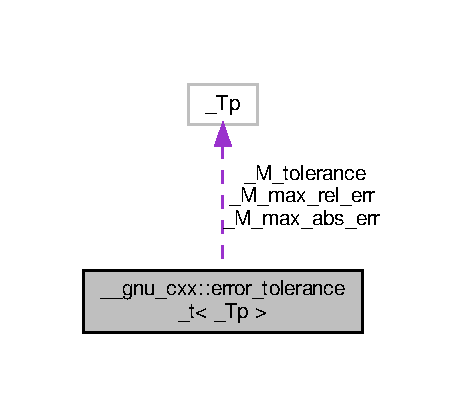
\includegraphics[width=223pt]{struct____gnu__cxx_1_1error__tolerance__t__coll__graph}
\end{center}
\end{figure}
\subsection*{Public Member Functions}
\begin{DoxyCompactItemize}
\item 
constexpr \hyperlink{struct____gnu__cxx_1_1error__tolerance__t_a4d33e75bacc130e0d0b3edbfdeaea975}{error\+\_\+tolerance\+\_\+t} (\hyperlink{namespace____gnu__cxx_a3b19a9c800ca194374ef9172290f7d79}{\+\_\+\+Tp} \+\_\+\+\_\+max\+\_\+abs\+\_\+err, \hyperlink{namespace____gnu__cxx_a3b19a9c800ca194374ef9172290f7d79}{\+\_\+\+Tp} \+\_\+\+\_\+max\+\_\+rel\+\_\+err, unsigned \+\_\+\+\_\+min\+\_\+num\+\_\+passes)
\item 
{\footnotesize template$<$typename \+\_\+\+Res\+Tp $>$ }\\\hyperlink{namespace____gnu__cxx_ae83aca57f97767d5d09188718728a0ac}{bool} \hyperlink{struct____gnu__cxx_1_1error__tolerance__t_a4376e70909c1b91fe98246a633162497}{test} (\+\_\+\+Res\+Tp \+\_\+\+\_\+curr\+\_\+result, \+\_\+\+Res\+Tp \+\_\+\+\_\+prev\+\_\+result)
\begin{DoxyCompactList}\small\item\em Return whether convergence is acceptable tolerance given two subsequent results. \end{DoxyCompactList}\item 
{\footnotesize template$<$typename \+\_\+\+Res\+Tp $>$ }\\constexpr \hyperlink{namespace____gnu__cxx_a3b19a9c800ca194374ef9172290f7d79}{\+\_\+\+Tp} \hyperlink{struct____gnu__cxx_1_1error__tolerance__t_a2564721b5a7aae5f2a74703dd4c5248a}{tolerance} (\+\_\+\+Res\+Tp \hyperlink{namespace____gnu__cxx_a500ea9f53aeaecd8c2ae657503450578}{\+\_\+\+\_\+result})
\begin{DoxyCompactList}\small\item\em Set and return the tolerance given an initial result. \end{DoxyCompactList}\item 
constexpr \hyperlink{namespace____gnu__cxx_a3b19a9c800ca194374ef9172290f7d79}{\+\_\+\+Tp} \hyperlink{struct____gnu__cxx_1_1error__tolerance__t_a938a772fb23ee5e7476dc9fba9a2d750}{tolerance} () const
\begin{DoxyCompactList}\small\item\em Return the current tolerance. \end{DoxyCompactList}\end{DoxyCompactItemize}
\subsection*{Static Public Member Functions}
\begin{DoxyCompactItemize}
\item 
static constexpr \hyperlink{namespace____gnu__cxx_ae83aca57f97767d5d09188718728a0ac}{bool} \hyperlink{struct____gnu__cxx_1_1error__tolerance__t_af17fb63ac7623ad0090241cff57b7492}{\+\_\+\+S\+\_\+valid\+\_\+tolerances} (\hyperlink{namespace____gnu__cxx_a3b19a9c800ca194374ef9172290f7d79}{\+\_\+\+Tp} \+\_\+\+\_\+max\+\_\+abs\+\_\+err, \hyperlink{namespace____gnu__cxx_a3b19a9c800ca194374ef9172290f7d79}{\+\_\+\+Tp} \+\_\+\+\_\+max\+\_\+rel\+\_\+err)
\begin{DoxyCompactList}\small\item\em Test for valid error tolerances. \end{DoxyCompactList}\end{DoxyCompactItemize}
\subsection*{Public Attributes}
\begin{DoxyCompactItemize}
\item 
\hyperlink{namespace____gnu__cxx_a3b19a9c800ca194374ef9172290f7d79}{\+\_\+\+Tp} \hyperlink{struct____gnu__cxx_1_1error__tolerance__t_a55773fc8e99f5906ba9a2b2f03a141fb}{\+\_\+\+M\+\_\+max\+\_\+abs\+\_\+err}
\begin{DoxyCompactList}\small\item\em Maximum absolute error tolerance. \end{DoxyCompactList}\item 
\hyperlink{namespace____gnu__cxx_a3b19a9c800ca194374ef9172290f7d79}{\+\_\+\+Tp} \hyperlink{struct____gnu__cxx_1_1error__tolerance__t_add7d7bfa6c6f5c36f50dde1497486e9e}{\+\_\+\+M\+\_\+max\+\_\+rel\+\_\+err}
\begin{DoxyCompactList}\small\item\em Maximum relative error tolerance. \end{DoxyCompactList}\item 
unsigned \hyperlink{struct____gnu__cxx_1_1error__tolerance__t_a395bb8004b293af143b531ec6de046f0}{\+\_\+\+M\+\_\+min\+\_\+num\+\_\+passes}
\begin{DoxyCompactList}\small\item\em Minimum number of consecutive passes before result is OK. \end{DoxyCompactList}\item 
unsigned \hyperlink{struct____gnu__cxx_1_1error__tolerance__t_aa3f36e75dc6dd3c6d8283ffa18f78056}{\+\_\+\+M\+\_\+num\+\_\+passes}
\begin{DoxyCompactList}\small\item\em Current number of passes. \end{DoxyCompactList}\item 
\hyperlink{namespace____gnu__cxx_a3b19a9c800ca194374ef9172290f7d79}{\+\_\+\+Tp} \hyperlink{struct____gnu__cxx_1_1error__tolerance__t_a261304757b9ff28304ee94d67405b2a6}{\+\_\+\+M\+\_\+tolerance} = this-\/$>$\hyperlink{struct____gnu__cxx_1_1error__tolerance__t_a2564721b5a7aae5f2a74703dd4c5248a}{tolerance}(\hyperlink{namespace____gnu__cxx_a3b19a9c800ca194374ef9172290f7d79}{\+\_\+\+Tp}\{1\})
\begin{DoxyCompactList}\small\item\em Current tolerance. \end{DoxyCompactList}\end{DoxyCompactItemize}


\subsection{Detailed Description}
\subsubsection*{template$<$typename \+\_\+\+Tp$>$\newline
struct \+\_\+\+\_\+gnu\+\_\+cxx\+::error\+\_\+tolerance\+\_\+t$<$ \+\_\+\+Tp $>$}

An error tolerance model for integrals. 

Definition at line 82 of file integration.\+h.



\subsection{Constructor \& Destructor Documentation}
\mbox{\Hypertarget{struct____gnu__cxx_1_1error__tolerance__t_a4d33e75bacc130e0d0b3edbfdeaea975}\label{struct____gnu__cxx_1_1error__tolerance__t_a4d33e75bacc130e0d0b3edbfdeaea975}} 
\index{\+\_\+\+\_\+gnu\+\_\+cxx\+::error\+\_\+tolerance\+\_\+t@{\+\_\+\+\_\+gnu\+\_\+cxx\+::error\+\_\+tolerance\+\_\+t}!error\+\_\+tolerance\+\_\+t@{error\+\_\+tolerance\+\_\+t}}
\index{error\+\_\+tolerance\+\_\+t@{error\+\_\+tolerance\+\_\+t}!\+\_\+\+\_\+gnu\+\_\+cxx\+::error\+\_\+tolerance\+\_\+t@{\+\_\+\+\_\+gnu\+\_\+cxx\+::error\+\_\+tolerance\+\_\+t}}
\subsubsection{\texorpdfstring{error\+\_\+tolerance\+\_\+t()}{error\_tolerance\_t()}}
{\footnotesize\ttfamily template$<$typename \+\_\+\+Tp $>$ \\
constexpr \hyperlink{struct____gnu__cxx_1_1error__tolerance__t}{\+\_\+\+\_\+gnu\+\_\+cxx\+::error\+\_\+tolerance\+\_\+t}$<$ \hyperlink{namespace____gnu__cxx_a3b19a9c800ca194374ef9172290f7d79}{\+\_\+\+Tp} $>$\+::\hyperlink{struct____gnu__cxx_1_1error__tolerance__t}{error\+\_\+tolerance\+\_\+t} (\begin{DoxyParamCaption}\item[{\hyperlink{namespace____gnu__cxx_a3b19a9c800ca194374ef9172290f7d79}{\+\_\+\+Tp}}]{\+\_\+\+\_\+max\+\_\+abs\+\_\+err,  }\item[{\hyperlink{namespace____gnu__cxx_a3b19a9c800ca194374ef9172290f7d79}{\+\_\+\+Tp}}]{\+\_\+\+\_\+max\+\_\+rel\+\_\+err,  }\item[{unsigned}]{\+\_\+\+\_\+min\+\_\+num\+\_\+passes }\end{DoxyParamCaption})}



\subsection{Member Function Documentation}
\mbox{\Hypertarget{struct____gnu__cxx_1_1error__tolerance__t_af17fb63ac7623ad0090241cff57b7492}\label{struct____gnu__cxx_1_1error__tolerance__t_af17fb63ac7623ad0090241cff57b7492}} 
\index{\+\_\+\+\_\+gnu\+\_\+cxx\+::error\+\_\+tolerance\+\_\+t@{\+\_\+\+\_\+gnu\+\_\+cxx\+::error\+\_\+tolerance\+\_\+t}!\+\_\+\+S\+\_\+valid\+\_\+tolerances@{\+\_\+\+S\+\_\+valid\+\_\+tolerances}}
\index{\+\_\+\+S\+\_\+valid\+\_\+tolerances@{\+\_\+\+S\+\_\+valid\+\_\+tolerances}!\+\_\+\+\_\+gnu\+\_\+cxx\+::error\+\_\+tolerance\+\_\+t@{\+\_\+\+\_\+gnu\+\_\+cxx\+::error\+\_\+tolerance\+\_\+t}}
\subsubsection{\texorpdfstring{\+\_\+\+S\+\_\+valid\+\_\+tolerances()}{\_S\_valid\_tolerances()}}
{\footnotesize\ttfamily template$<$typename \+\_\+\+Tp $>$ \\
static constexpr \hyperlink{namespace____gnu__cxx_ae83aca57f97767d5d09188718728a0ac}{bool} \hyperlink{struct____gnu__cxx_1_1error__tolerance__t}{\+\_\+\+\_\+gnu\+\_\+cxx\+::error\+\_\+tolerance\+\_\+t}$<$ \hyperlink{namespace____gnu__cxx_a3b19a9c800ca194374ef9172290f7d79}{\+\_\+\+Tp} $>$\+::\+\_\+\+S\+\_\+valid\+\_\+tolerances (\begin{DoxyParamCaption}\item[{\hyperlink{namespace____gnu__cxx_a3b19a9c800ca194374ef9172290f7d79}{\+\_\+\+Tp}}]{\+\_\+\+\_\+max\+\_\+abs\+\_\+err,  }\item[{\hyperlink{namespace____gnu__cxx_a3b19a9c800ca194374ef9172290f7d79}{\+\_\+\+Tp}}]{\+\_\+\+\_\+max\+\_\+rel\+\_\+err }\end{DoxyParamCaption})\hspace{0.3cm}{\ttfamily [inline]}, {\ttfamily [static]}}



Test for valid error tolerances. 



Definition at line 132 of file integration.\+h.



References \+\_\+\+\_\+gnu\+\_\+cxx\+::\+\_\+\+Tp.



Referenced by \+\_\+\+\_\+gnu\+\_\+cxx\+::valid\+\_\+tolerances().


\begin{DoxyCode}
133       \{
134         constexpr \textcolor{keyword}{auto} \_S\_eps = std::numeric\_limits<\_Tp>::epsilon();
135         \textcolor{keywordflow}{return} !(\_\_max\_abs\_err <= \hyperlink{namespace____gnu__cxx_a3b19a9c800ca194374ef9172290f7d79}{\_Tp}\{0\}
136               && (\_\_max\_rel\_err < \hyperlink{namespace____gnu__cxx_a3b19a9c800ca194374ef9172290f7d79}{\_Tp}\{50\} * \_S\_eps
137                || \_\_max\_rel\_err < 0.5e-28));
138         \textcolor{comment}{// I don't understand the etymology of this last number.}
139       \}
\end{DoxyCode}
\mbox{\Hypertarget{struct____gnu__cxx_1_1error__tolerance__t_a4376e70909c1b91fe98246a633162497}\label{struct____gnu__cxx_1_1error__tolerance__t_a4376e70909c1b91fe98246a633162497}} 
\index{\+\_\+\+\_\+gnu\+\_\+cxx\+::error\+\_\+tolerance\+\_\+t@{\+\_\+\+\_\+gnu\+\_\+cxx\+::error\+\_\+tolerance\+\_\+t}!test@{test}}
\index{test@{test}!\+\_\+\+\_\+gnu\+\_\+cxx\+::error\+\_\+tolerance\+\_\+t@{\+\_\+\+\_\+gnu\+\_\+cxx\+::error\+\_\+tolerance\+\_\+t}}
\subsubsection{\texorpdfstring{test()}{test()}}
{\footnotesize\ttfamily template$<$typename \+\_\+\+Tp $>$ \\
template$<$typename \+\_\+\+Res\+Tp $>$ \\
\hyperlink{namespace____gnu__cxx_ae83aca57f97767d5d09188718728a0ac}{bool} \hyperlink{struct____gnu__cxx_1_1error__tolerance__t}{\+\_\+\+\_\+gnu\+\_\+cxx\+::error\+\_\+tolerance\+\_\+t}$<$ \hyperlink{namespace____gnu__cxx_a3b19a9c800ca194374ef9172290f7d79}{\+\_\+\+Tp} $>$\+::test (\begin{DoxyParamCaption}\item[{\+\_\+\+Res\+Tp}]{\+\_\+\+\_\+curr\+\_\+result,  }\item[{\+\_\+\+Res\+Tp}]{\+\_\+\+\_\+prev\+\_\+result }\end{DoxyParamCaption})\hspace{0.3cm}{\ttfamily [inline]}}



Return whether convergence is acceptable tolerance given two subsequent results. 



Definition at line 114 of file integration.\+h.



References \+\_\+\+\_\+gnu\+\_\+cxx\+::\+\_\+\+Tp.


\begin{DoxyCode}
115         \{
116           \textcolor{keyword}{const} \textcolor{keyword}{auto} \_\_del = std::abs(\_\_curr\_result - \_\_prev\_result);
117           \textcolor{keywordflow}{if} (\_\_del < this->\hyperlink{struct____gnu__cxx_1_1error__tolerance__t_a55773fc8e99f5906ba9a2b2f03a141fb}{\_M\_max\_abs\_err}
118               || \_\_del < this->\hyperlink{struct____gnu__cxx_1_1error__tolerance__t_add7d7bfa6c6f5c36f50dde1497486e9e}{\_M\_max\_rel\_err} * std::abs(\_\_curr\_result))
119             ++this->\hyperlink{struct____gnu__cxx_1_1error__tolerance__t_aa3f36e75dc6dd3c6d8283ffa18f78056}{\_M\_num\_passes};
120           \textcolor{keywordflow}{else}
121             this->\hyperlink{struct____gnu__cxx_1_1error__tolerance__t_aa3f36e75dc6dd3c6d8283ffa18f78056}{\_M\_num\_passes} = 0;
122           \textcolor{keywordflow}{return} this->\hyperlink{struct____gnu__cxx_1_1error__tolerance__t_aa3f36e75dc6dd3c6d8283ffa18f78056}{\_M\_num\_passes} >= this->\hyperlink{struct____gnu__cxx_1_1error__tolerance__t_a395bb8004b293af143b531ec6de046f0}{\_M\_min\_num\_passes};
123         \}
\end{DoxyCode}
\mbox{\Hypertarget{struct____gnu__cxx_1_1error__tolerance__t_a2564721b5a7aae5f2a74703dd4c5248a}\label{struct____gnu__cxx_1_1error__tolerance__t_a2564721b5a7aae5f2a74703dd4c5248a}} 
\index{\+\_\+\+\_\+gnu\+\_\+cxx\+::error\+\_\+tolerance\+\_\+t@{\+\_\+\+\_\+gnu\+\_\+cxx\+::error\+\_\+tolerance\+\_\+t}!tolerance@{tolerance}}
\index{tolerance@{tolerance}!\+\_\+\+\_\+gnu\+\_\+cxx\+::error\+\_\+tolerance\+\_\+t@{\+\_\+\+\_\+gnu\+\_\+cxx\+::error\+\_\+tolerance\+\_\+t}}
\subsubsection{\texorpdfstring{tolerance()}{tolerance()}\hspace{0.1cm}{\footnotesize\ttfamily [1/2]}}
{\footnotesize\ttfamily template$<$typename \+\_\+\+Tp $>$ \\
template$<$typename \+\_\+\+Res\+Tp $>$ \\
constexpr \hyperlink{namespace____gnu__cxx_a3b19a9c800ca194374ef9172290f7d79}{\+\_\+\+Tp} \hyperlink{struct____gnu__cxx_1_1error__tolerance__t}{\+\_\+\+\_\+gnu\+\_\+cxx\+::error\+\_\+tolerance\+\_\+t}$<$ \hyperlink{namespace____gnu__cxx_a3b19a9c800ca194374ef9172290f7d79}{\+\_\+\+Tp} $>$\+::tolerance (\begin{DoxyParamCaption}\item[{\+\_\+\+Res\+Tp}]{\+\_\+\+\_\+result }\end{DoxyParamCaption})\hspace{0.3cm}{\ttfamily [inline]}}



Set and return the tolerance given an initial result. 



Definition at line 102 of file integration.\+h.



References \+\_\+\+\_\+gnu\+\_\+cxx\+::\+\_\+\+Tp.


\begin{DoxyCode}
103         \{
104           this->\hyperlink{struct____gnu__cxx_1_1error__tolerance__t_a261304757b9ff28304ee94d67405b2a6}{\_M\_tolerance}
105                   = std::max(this->\hyperlink{struct____gnu__cxx_1_1error__tolerance__t_a55773fc8e99f5906ba9a2b2f03a141fb}{\_M\_max\_abs\_err},
106                              \hyperlink{namespace____gnu__cxx_a3b19a9c800ca194374ef9172290f7d79}{\_Tp}(this->\hyperlink{struct____gnu__cxx_1_1error__tolerance__t_add7d7bfa6c6f5c36f50dde1497486e9e}{\_M\_max\_rel\_err} * std::abs(
      \hyperlink{namespace____gnu__cxx_a500ea9f53aeaecd8c2ae657503450578}{\_\_result})));
107           \textcolor{keywordflow}{return} this->\hyperlink{struct____gnu__cxx_1_1error__tolerance__t_a261304757b9ff28304ee94d67405b2a6}{\_M\_tolerance};
108         \}
\end{DoxyCode}
\mbox{\Hypertarget{struct____gnu__cxx_1_1error__tolerance__t_a938a772fb23ee5e7476dc9fba9a2d750}\label{struct____gnu__cxx_1_1error__tolerance__t_a938a772fb23ee5e7476dc9fba9a2d750}} 
\index{\+\_\+\+\_\+gnu\+\_\+cxx\+::error\+\_\+tolerance\+\_\+t@{\+\_\+\+\_\+gnu\+\_\+cxx\+::error\+\_\+tolerance\+\_\+t}!tolerance@{tolerance}}
\index{tolerance@{tolerance}!\+\_\+\+\_\+gnu\+\_\+cxx\+::error\+\_\+tolerance\+\_\+t@{\+\_\+\+\_\+gnu\+\_\+cxx\+::error\+\_\+tolerance\+\_\+t}}
\subsubsection{\texorpdfstring{tolerance()}{tolerance()}\hspace{0.1cm}{\footnotesize\ttfamily [2/2]}}
{\footnotesize\ttfamily template$<$typename \+\_\+\+Tp $>$ \\
constexpr \hyperlink{namespace____gnu__cxx_a3b19a9c800ca194374ef9172290f7d79}{\+\_\+\+Tp} \hyperlink{struct____gnu__cxx_1_1error__tolerance__t}{\+\_\+\+\_\+gnu\+\_\+cxx\+::error\+\_\+tolerance\+\_\+t}$<$ \hyperlink{namespace____gnu__cxx_a3b19a9c800ca194374ef9172290f7d79}{\+\_\+\+Tp} $>$\+::tolerance (\begin{DoxyParamCaption}{ }\end{DoxyParamCaption}) const\hspace{0.3cm}{\ttfamily [inline]}}



Return the current tolerance. 



Definition at line 127 of file integration.\+h.


\begin{DoxyCode}
128       \{ \textcolor{keywordflow}{return} this->\hyperlink{struct____gnu__cxx_1_1error__tolerance__t_a261304757b9ff28304ee94d67405b2a6}{\_M\_tolerance}; \}
\end{DoxyCode}


\subsection{Member Data Documentation}
\mbox{\Hypertarget{struct____gnu__cxx_1_1error__tolerance__t_a55773fc8e99f5906ba9a2b2f03a141fb}\label{struct____gnu__cxx_1_1error__tolerance__t_a55773fc8e99f5906ba9a2b2f03a141fb}} 
\index{\+\_\+\+\_\+gnu\+\_\+cxx\+::error\+\_\+tolerance\+\_\+t@{\+\_\+\+\_\+gnu\+\_\+cxx\+::error\+\_\+tolerance\+\_\+t}!\+\_\+\+M\+\_\+max\+\_\+abs\+\_\+err@{\+\_\+\+M\+\_\+max\+\_\+abs\+\_\+err}}
\index{\+\_\+\+M\+\_\+max\+\_\+abs\+\_\+err@{\+\_\+\+M\+\_\+max\+\_\+abs\+\_\+err}!\+\_\+\+\_\+gnu\+\_\+cxx\+::error\+\_\+tolerance\+\_\+t@{\+\_\+\+\_\+gnu\+\_\+cxx\+::error\+\_\+tolerance\+\_\+t}}
\subsubsection{\texorpdfstring{\+\_\+\+M\+\_\+max\+\_\+abs\+\_\+err}{\_M\_max\_abs\_err}}
{\footnotesize\ttfamily template$<$typename \+\_\+\+Tp $>$ \\
\hyperlink{namespace____gnu__cxx_a3b19a9c800ca194374ef9172290f7d79}{\+\_\+\+Tp} \hyperlink{struct____gnu__cxx_1_1error__tolerance__t}{\+\_\+\+\_\+gnu\+\_\+cxx\+::error\+\_\+tolerance\+\_\+t}$<$ \hyperlink{namespace____gnu__cxx_a3b19a9c800ca194374ef9172290f7d79}{\+\_\+\+Tp} $>$\+::\+\_\+\+M\+\_\+max\+\_\+abs\+\_\+err}



Maximum absolute error tolerance. 



Definition at line 89 of file integration.\+h.

\mbox{\Hypertarget{struct____gnu__cxx_1_1error__tolerance__t_add7d7bfa6c6f5c36f50dde1497486e9e}\label{struct____gnu__cxx_1_1error__tolerance__t_add7d7bfa6c6f5c36f50dde1497486e9e}} 
\index{\+\_\+\+\_\+gnu\+\_\+cxx\+::error\+\_\+tolerance\+\_\+t@{\+\_\+\+\_\+gnu\+\_\+cxx\+::error\+\_\+tolerance\+\_\+t}!\+\_\+\+M\+\_\+max\+\_\+rel\+\_\+err@{\+\_\+\+M\+\_\+max\+\_\+rel\+\_\+err}}
\index{\+\_\+\+M\+\_\+max\+\_\+rel\+\_\+err@{\+\_\+\+M\+\_\+max\+\_\+rel\+\_\+err}!\+\_\+\+\_\+gnu\+\_\+cxx\+::error\+\_\+tolerance\+\_\+t@{\+\_\+\+\_\+gnu\+\_\+cxx\+::error\+\_\+tolerance\+\_\+t}}
\subsubsection{\texorpdfstring{\+\_\+\+M\+\_\+max\+\_\+rel\+\_\+err}{\_M\_max\_rel\_err}}
{\footnotesize\ttfamily template$<$typename \+\_\+\+Tp $>$ \\
\hyperlink{namespace____gnu__cxx_a3b19a9c800ca194374ef9172290f7d79}{\+\_\+\+Tp} \hyperlink{struct____gnu__cxx_1_1error__tolerance__t}{\+\_\+\+\_\+gnu\+\_\+cxx\+::error\+\_\+tolerance\+\_\+t}$<$ \hyperlink{namespace____gnu__cxx_a3b19a9c800ca194374ef9172290f7d79}{\+\_\+\+Tp} $>$\+::\+\_\+\+M\+\_\+max\+\_\+rel\+\_\+err}



Maximum relative error tolerance. 



Definition at line 91 of file integration.\+h.

\mbox{\Hypertarget{struct____gnu__cxx_1_1error__tolerance__t_a395bb8004b293af143b531ec6de046f0}\label{struct____gnu__cxx_1_1error__tolerance__t_a395bb8004b293af143b531ec6de046f0}} 
\index{\+\_\+\+\_\+gnu\+\_\+cxx\+::error\+\_\+tolerance\+\_\+t@{\+\_\+\+\_\+gnu\+\_\+cxx\+::error\+\_\+tolerance\+\_\+t}!\+\_\+\+M\+\_\+min\+\_\+num\+\_\+passes@{\+\_\+\+M\+\_\+min\+\_\+num\+\_\+passes}}
\index{\+\_\+\+M\+\_\+min\+\_\+num\+\_\+passes@{\+\_\+\+M\+\_\+min\+\_\+num\+\_\+passes}!\+\_\+\+\_\+gnu\+\_\+cxx\+::error\+\_\+tolerance\+\_\+t@{\+\_\+\+\_\+gnu\+\_\+cxx\+::error\+\_\+tolerance\+\_\+t}}
\subsubsection{\texorpdfstring{\+\_\+\+M\+\_\+min\+\_\+num\+\_\+passes}{\_M\_min\_num\_passes}}
{\footnotesize\ttfamily template$<$typename \+\_\+\+Tp $>$ \\
unsigned \hyperlink{struct____gnu__cxx_1_1error__tolerance__t}{\+\_\+\+\_\+gnu\+\_\+cxx\+::error\+\_\+tolerance\+\_\+t}$<$ \hyperlink{namespace____gnu__cxx_a3b19a9c800ca194374ef9172290f7d79}{\+\_\+\+Tp} $>$\+::\+\_\+\+M\+\_\+min\+\_\+num\+\_\+passes}



Minimum number of consecutive passes before result is OK. 



Definition at line 95 of file integration.\+h.

\mbox{\Hypertarget{struct____gnu__cxx_1_1error__tolerance__t_aa3f36e75dc6dd3c6d8283ffa18f78056}\label{struct____gnu__cxx_1_1error__tolerance__t_aa3f36e75dc6dd3c6d8283ffa18f78056}} 
\index{\+\_\+\+\_\+gnu\+\_\+cxx\+::error\+\_\+tolerance\+\_\+t@{\+\_\+\+\_\+gnu\+\_\+cxx\+::error\+\_\+tolerance\+\_\+t}!\+\_\+\+M\+\_\+num\+\_\+passes@{\+\_\+\+M\+\_\+num\+\_\+passes}}
\index{\+\_\+\+M\+\_\+num\+\_\+passes@{\+\_\+\+M\+\_\+num\+\_\+passes}!\+\_\+\+\_\+gnu\+\_\+cxx\+::error\+\_\+tolerance\+\_\+t@{\+\_\+\+\_\+gnu\+\_\+cxx\+::error\+\_\+tolerance\+\_\+t}}
\subsubsection{\texorpdfstring{\+\_\+\+M\+\_\+num\+\_\+passes}{\_M\_num\_passes}}
{\footnotesize\ttfamily template$<$typename \+\_\+\+Tp $>$ \\
unsigned \hyperlink{struct____gnu__cxx_1_1error__tolerance__t}{\+\_\+\+\_\+gnu\+\_\+cxx\+::error\+\_\+tolerance\+\_\+t}$<$ \hyperlink{namespace____gnu__cxx_a3b19a9c800ca194374ef9172290f7d79}{\+\_\+\+Tp} $>$\+::\+\_\+\+M\+\_\+num\+\_\+passes}



Current number of passes. 



Definition at line 97 of file integration.\+h.

\mbox{\Hypertarget{struct____gnu__cxx_1_1error__tolerance__t_a261304757b9ff28304ee94d67405b2a6}\label{struct____gnu__cxx_1_1error__tolerance__t_a261304757b9ff28304ee94d67405b2a6}} 
\index{\+\_\+\+\_\+gnu\+\_\+cxx\+::error\+\_\+tolerance\+\_\+t@{\+\_\+\+\_\+gnu\+\_\+cxx\+::error\+\_\+tolerance\+\_\+t}!\+\_\+\+M\+\_\+tolerance@{\+\_\+\+M\+\_\+tolerance}}
\index{\+\_\+\+M\+\_\+tolerance@{\+\_\+\+M\+\_\+tolerance}!\+\_\+\+\_\+gnu\+\_\+cxx\+::error\+\_\+tolerance\+\_\+t@{\+\_\+\+\_\+gnu\+\_\+cxx\+::error\+\_\+tolerance\+\_\+t}}
\subsubsection{\texorpdfstring{\+\_\+\+M\+\_\+tolerance}{\_M\_tolerance}}
{\footnotesize\ttfamily template$<$typename \+\_\+\+Tp $>$ \\
\hyperlink{namespace____gnu__cxx_a3b19a9c800ca194374ef9172290f7d79}{\+\_\+\+Tp} \hyperlink{struct____gnu__cxx_1_1error__tolerance__t}{\+\_\+\+\_\+gnu\+\_\+cxx\+::error\+\_\+tolerance\+\_\+t}$<$ \hyperlink{namespace____gnu__cxx_a3b19a9c800ca194374ef9172290f7d79}{\+\_\+\+Tp} $>$\+::\+\_\+\+M\+\_\+tolerance = this-\/$>$\hyperlink{struct____gnu__cxx_1_1error__tolerance__t_a2564721b5a7aae5f2a74703dd4c5248a}{tolerance}(\hyperlink{namespace____gnu__cxx_a3b19a9c800ca194374ef9172290f7d79}{\+\_\+\+Tp}\{1\})}



Current tolerance. 



Definition at line 93 of file integration.\+h.



The documentation for this struct was generated from the following file\+:\begin{DoxyCompactItemize}
\item 
include/ext/\hyperlink{integration_8h}{integration.\+h}\end{DoxyCompactItemize}

\hypertarget{class____gnu__cxx_1_1extrapolation__table}{}\section{\+\_\+\+\_\+gnu\+\_\+cxx\+:\+:extrapolation\+\_\+table$<$ \+\_\+\+Tp $>$ Class Template Reference}
\label{class____gnu__cxx_1_1extrapolation__table}\index{\+\_\+\+\_\+gnu\+\_\+cxx\+::extrapolation\+\_\+table$<$ \+\_\+\+Tp $>$@{\+\_\+\+\_\+gnu\+\_\+cxx\+::extrapolation\+\_\+table$<$ \+\_\+\+Tp $>$}}


{\ttfamily \#include $<$extrapolation\+\_\+table.\+h$>$}

\subsection*{Public Member Functions}
\begin{DoxyCompactItemize}
\item 
\hyperlink{class____gnu__cxx_1_1extrapolation__table_a7769d0bb61a2b5b0153140d707b2d3a0}{extrapolation\+\_\+table} ()
\item 
\hyperlink{class____gnu__cxx_1_1extrapolation__table_a9866afc5e42c63b300e21620ad8adac2}{extrapolation\+\_\+table} (\hyperlink{namespace____gnu__cxx_a3b19a9c800ca194374ef9172290f7d79}{\+\_\+\+Tp} \+\_\+\+\_\+y)
\item 
void \hyperlink{class____gnu__cxx_1_1extrapolation__table_a0a20b6d8a3c194a962ce6f1bba96f5e9}{append} (\hyperlink{namespace____gnu__cxx_a3b19a9c800ca194374ef9172290f7d79}{\+\_\+\+Tp} \+\_\+\+\_\+y)
\item 
std\+::size\+\_\+t \hyperlink{class____gnu__cxx_1_1extrapolation__table_a4948ba62ca85ddecc2b530096b368908}{get\+\_\+nn} () const
\item 
std\+::tuple$<$ \hyperlink{namespace____gnu__cxx_a3b19a9c800ca194374ef9172290f7d79}{\+\_\+\+Tp}, \hyperlink{namespace____gnu__cxx_a3b19a9c800ca194374ef9172290f7d79}{\+\_\+\+Tp} $>$ \hyperlink{class____gnu__cxx_1_1extrapolation__table_a8bacdbca35a9df35185102710380a8ec}{qelg} ()
\end{DoxyCompactItemize}


\subsection{Detailed Description}
\subsubsection*{template$<$typename \+\_\+\+Tp$>$\newline
class \+\_\+\+\_\+gnu\+\_\+cxx\+::extrapolation\+\_\+table$<$ \+\_\+\+Tp $>$}



Definition at line 40 of file extrapolation\+\_\+table.\+h.



\subsection{Constructor \& Destructor Documentation}
\mbox{\Hypertarget{class____gnu__cxx_1_1extrapolation__table_a7769d0bb61a2b5b0153140d707b2d3a0}\label{class____gnu__cxx_1_1extrapolation__table_a7769d0bb61a2b5b0153140d707b2d3a0}} 
\index{\+\_\+\+\_\+gnu\+\_\+cxx\+::extrapolation\+\_\+table@{\+\_\+\+\_\+gnu\+\_\+cxx\+::extrapolation\+\_\+table}!extrapolation\+\_\+table@{extrapolation\+\_\+table}}
\index{extrapolation\+\_\+table@{extrapolation\+\_\+table}!\+\_\+\+\_\+gnu\+\_\+cxx\+::extrapolation\+\_\+table@{\+\_\+\+\_\+gnu\+\_\+cxx\+::extrapolation\+\_\+table}}
\subsubsection{\texorpdfstring{extrapolation\+\_\+table()}{extrapolation\_table()}\hspace{0.1cm}{\footnotesize\ttfamily [1/2]}}
{\footnotesize\ttfamily template$<$typename \+\_\+\+Tp$>$ \\
\hyperlink{class____gnu__cxx_1_1extrapolation__table}{\+\_\+\+\_\+gnu\+\_\+cxx\+::extrapolation\+\_\+table}$<$ \hyperlink{namespace____gnu__cxx_a3b19a9c800ca194374ef9172290f7d79}{\+\_\+\+Tp} $>$\+::\hyperlink{class____gnu__cxx_1_1extrapolation__table}{extrapolation\+\_\+table} (\begin{DoxyParamCaption}{ }\end{DoxyParamCaption})\hspace{0.3cm}{\ttfamily [inline]}}



Definition at line 54 of file extrapolation\+\_\+table.\+h.


\begin{DoxyCode}
55       : \_M\_nn(0),
56         \_M\_nres(0)
57       \{
58         \textcolor{comment}{// Try to adjust tests for varing precision?}
59         \textcolor{comment}{// I don't think this is a precision-sensitive limit.}
60         \textcolor{comment}{//this->\_M\_irreg\_test = std::pow(10.0,}
61         \textcolor{comment}{//                       -std::numeric\_limits<\_Tp>::digits10 / 4.0);}
62       \}
\end{DoxyCode}
\mbox{\Hypertarget{class____gnu__cxx_1_1extrapolation__table_a9866afc5e42c63b300e21620ad8adac2}\label{class____gnu__cxx_1_1extrapolation__table_a9866afc5e42c63b300e21620ad8adac2}} 
\index{\+\_\+\+\_\+gnu\+\_\+cxx\+::extrapolation\+\_\+table@{\+\_\+\+\_\+gnu\+\_\+cxx\+::extrapolation\+\_\+table}!extrapolation\+\_\+table@{extrapolation\+\_\+table}}
\index{extrapolation\+\_\+table@{extrapolation\+\_\+table}!\+\_\+\+\_\+gnu\+\_\+cxx\+::extrapolation\+\_\+table@{\+\_\+\+\_\+gnu\+\_\+cxx\+::extrapolation\+\_\+table}}
\subsubsection{\texorpdfstring{extrapolation\+\_\+table()}{extrapolation\_table()}\hspace{0.1cm}{\footnotesize\ttfamily [2/2]}}
{\footnotesize\ttfamily template$<$typename \+\_\+\+Tp$>$ \\
\hyperlink{class____gnu__cxx_1_1extrapolation__table}{\+\_\+\+\_\+gnu\+\_\+cxx\+::extrapolation\+\_\+table}$<$ \hyperlink{namespace____gnu__cxx_a3b19a9c800ca194374ef9172290f7d79}{\+\_\+\+Tp} $>$\+::\hyperlink{class____gnu__cxx_1_1extrapolation__table}{extrapolation\+\_\+table} (\begin{DoxyParamCaption}\item[{\hyperlink{namespace____gnu__cxx_a3b19a9c800ca194374ef9172290f7d79}{\+\_\+\+Tp}}]{\+\_\+\+\_\+y }\end{DoxyParamCaption})\hspace{0.3cm}{\ttfamily [inline]}, {\ttfamily [explicit]}}



Definition at line 64 of file extrapolation\+\_\+table.\+h.



References \+\_\+\+\_\+gnu\+\_\+cxx\+::extrapolation\+\_\+table$<$ \+\_\+\+Tp $>$\+::append().


\begin{DoxyCode}
65       : \_M\_nn(0),
66         \_M\_nres(0)
67       \{ this->\hyperlink{class____gnu__cxx_1_1extrapolation__table_a0a20b6d8a3c194a962ce6f1bba96f5e9}{append}(\_\_y); \}
\end{DoxyCode}


\subsection{Member Function Documentation}
\mbox{\Hypertarget{class____gnu__cxx_1_1extrapolation__table_a0a20b6d8a3c194a962ce6f1bba96f5e9}\label{class____gnu__cxx_1_1extrapolation__table_a0a20b6d8a3c194a962ce6f1bba96f5e9}} 
\index{\+\_\+\+\_\+gnu\+\_\+cxx\+::extrapolation\+\_\+table@{\+\_\+\+\_\+gnu\+\_\+cxx\+::extrapolation\+\_\+table}!append@{append}}
\index{append@{append}!\+\_\+\+\_\+gnu\+\_\+cxx\+::extrapolation\+\_\+table@{\+\_\+\+\_\+gnu\+\_\+cxx\+::extrapolation\+\_\+table}}
\subsubsection{\texorpdfstring{append()}{append()}}
{\footnotesize\ttfamily template$<$typename \+\_\+\+Tp$>$ \\
void \hyperlink{class____gnu__cxx_1_1extrapolation__table}{\+\_\+\+\_\+gnu\+\_\+cxx\+::extrapolation\+\_\+table}$<$ \hyperlink{namespace____gnu__cxx_a3b19a9c800ca194374ef9172290f7d79}{\+\_\+\+Tp} $>$\+::append (\begin{DoxyParamCaption}\item[{\hyperlink{namespace____gnu__cxx_a3b19a9c800ca194374ef9172290f7d79}{\+\_\+\+Tp}}]{\+\_\+\+\_\+y }\end{DoxyParamCaption})\hspace{0.3cm}{\ttfamily [inline]}}



Definition at line 70 of file extrapolation\+\_\+table.\+h.



References \+\_\+\+\_\+gnu\+\_\+cxx\+::extrapolation\+\_\+table$<$ \+\_\+\+Tp $>$\+::qelg().



Referenced by \+\_\+\+\_\+gnu\+\_\+cxx\+::extrapolation\+\_\+table$<$ \+\_\+\+Tp $>$\+::extrapolation\+\_\+table(), \+\_\+\+\_\+gnu\+\_\+cxx\+::qagp\+\_\+integrate(), \+\_\+\+\_\+gnu\+\_\+cxx\+::qags\+\_\+integrate(), \+\_\+\+\_\+gnu\+\_\+cxx\+::qawf\+\_\+integrate(), and \+\_\+\+\_\+gnu\+\_\+cxx\+::qawo\+\_\+integrate().


\begin{DoxyCode}
71       \{
72         \textcolor{keywordflow}{if} (this->\_M\_nn < this->\_M\_rlist2.size())
73           \{
74             this->\_M\_rlist2[this->\_M\_nn] = \_\_y;
75             ++this->\_M\_nn;
76           \}
77       \}
\end{DoxyCode}
\mbox{\Hypertarget{class____gnu__cxx_1_1extrapolation__table_a4948ba62ca85ddecc2b530096b368908}\label{class____gnu__cxx_1_1extrapolation__table_a4948ba62ca85ddecc2b530096b368908}} 
\index{\+\_\+\+\_\+gnu\+\_\+cxx\+::extrapolation\+\_\+table@{\+\_\+\+\_\+gnu\+\_\+cxx\+::extrapolation\+\_\+table}!get\+\_\+nn@{get\+\_\+nn}}
\index{get\+\_\+nn@{get\+\_\+nn}!\+\_\+\+\_\+gnu\+\_\+cxx\+::extrapolation\+\_\+table@{\+\_\+\+\_\+gnu\+\_\+cxx\+::extrapolation\+\_\+table}}
\subsubsection{\texorpdfstring{get\+\_\+nn()}{get\_nn()}}
{\footnotesize\ttfamily template$<$typename \+\_\+\+Tp$>$ \\
std\+::size\+\_\+t \hyperlink{class____gnu__cxx_1_1extrapolation__table}{\+\_\+\+\_\+gnu\+\_\+cxx\+::extrapolation\+\_\+table}$<$ \hyperlink{namespace____gnu__cxx_a3b19a9c800ca194374ef9172290f7d79}{\+\_\+\+Tp} $>$\+::get\+\_\+nn (\begin{DoxyParamCaption}{ }\end{DoxyParamCaption}) const\hspace{0.3cm}{\ttfamily [inline]}}



Definition at line 83 of file extrapolation\+\_\+table.\+h.



Referenced by \+\_\+\+\_\+gnu\+\_\+cxx\+::qagp\+\_\+integrate(), \+\_\+\+\_\+gnu\+\_\+cxx\+::qags\+\_\+integrate(), \+\_\+\+\_\+gnu\+\_\+cxx\+::qawf\+\_\+integrate(), and \+\_\+\+\_\+gnu\+\_\+cxx\+::qawo\+\_\+integrate().


\begin{DoxyCode}
84       \{ \textcolor{keywordflow}{return} this->\_M\_nn; \}
\end{DoxyCode}
\mbox{\Hypertarget{class____gnu__cxx_1_1extrapolation__table_a8bacdbca35a9df35185102710380a8ec}\label{class____gnu__cxx_1_1extrapolation__table_a8bacdbca35a9df35185102710380a8ec}} 
\index{\+\_\+\+\_\+gnu\+\_\+cxx\+::extrapolation\+\_\+table@{\+\_\+\+\_\+gnu\+\_\+cxx\+::extrapolation\+\_\+table}!qelg@{qelg}}
\index{qelg@{qelg}!\+\_\+\+\_\+gnu\+\_\+cxx\+::extrapolation\+\_\+table@{\+\_\+\+\_\+gnu\+\_\+cxx\+::extrapolation\+\_\+table}}
\subsubsection{\texorpdfstring{qelg()}{qelg()}}
{\footnotesize\ttfamily template$<$typename \+\_\+\+Tp $>$ \\
std\+::tuple$<$ \hyperlink{namespace____gnu__cxx_a3b19a9c800ca194374ef9172290f7d79}{\+\_\+\+Tp}, \hyperlink{namespace____gnu__cxx_a3b19a9c800ca194374ef9172290f7d79}{\+\_\+\+Tp} $>$ \hyperlink{class____gnu__cxx_1_1extrapolation__table}{\+\_\+\+\_\+gnu\+\_\+cxx\+::extrapolation\+\_\+table}$<$ \hyperlink{namespace____gnu__cxx_a3b19a9c800ca194374ef9172290f7d79}{\+\_\+\+Tp} $>$\+::qelg (\begin{DoxyParamCaption}{ }\end{DoxyParamCaption})}



Definition at line 35 of file extrapolation\+\_\+table.\+tcc.



References \+\_\+\+\_\+gnu\+\_\+cxx\+::\+\_\+\+\_\+abserr, \+\_\+\+\_\+gnu\+\_\+cxx\+::\+\_\+\+\_\+result, and \+\_\+\+\_\+gnu\+\_\+cxx\+::\+\_\+\+Tp.



Referenced by \+\_\+\+\_\+gnu\+\_\+cxx\+::extrapolation\+\_\+table$<$ \+\_\+\+Tp $>$\+::append(), \+\_\+\+\_\+gnu\+\_\+cxx\+::qagp\+\_\+integrate(), \+\_\+\+\_\+gnu\+\_\+cxx\+::qags\+\_\+integrate(), \+\_\+\+\_\+gnu\+\_\+cxx\+::qawf\+\_\+integrate(), and \+\_\+\+\_\+gnu\+\_\+cxx\+::qawo\+\_\+integrate().


\begin{DoxyCode}
36     \{
37       \textcolor{keyword}{const} \textcolor{keyword}{auto} \_\_cur\_n = this->\_M\_nn - 1;
38       \textcolor{keyword}{const} \textcolor{keyword}{auto} \_\_current = this->\_M\_rlist2[\_\_cur\_n];
39 
40       \textcolor{keyword}{const} \textcolor{keyword}{auto} \_S\_eps = std::numeric\_limits<\_Tp>::epsilon();
41       \textcolor{comment}{// Less than max to prevent overflow.}
42       \textcolor{keyword}{const} \textcolor{keyword}{auto} \_S\_max = std::numeric\_limits<\_Tp>::max() / \hyperlink{namespace____gnu__cxx_a3b19a9c800ca194374ef9172290f7d79}{\_Tp}\{100\};
43 
44       \textcolor{keyword}{auto} \_\_absolute = \_S\_max;
45       \textcolor{keyword}{auto} \_\_relative = 5 * \_S\_eps * std::abs(\_\_current);
46 
47       \textcolor{keyword}{const} \textcolor{keyword}{auto} \_\_newelm = \_\_cur\_n / 2;
48       \textcolor{keyword}{const} \textcolor{keyword}{auto} \_\_n\_orig = \_\_cur\_n;
49       \textcolor{keyword}{auto} \_\_n\_final = \_\_cur\_n;
50 
51       \textcolor{keyword}{const} \textcolor{keyword}{auto} \_\_nres\_orig = this->\_M\_nres;
52 
53       \textcolor{keyword}{auto} \hyperlink{namespace____gnu__cxx_a500ea9f53aeaecd8c2ae657503450578}{\_\_result} = \_\_current;
54       \textcolor{keyword}{auto} \hyperlink{namespace____gnu__cxx_a72f736cff127f1574e91a301de9e074b}{\_\_abserr} = \_S\_max;
55 
56       \textcolor{keywordflow}{if} (\_\_cur\_n < 2)
57         \{
58           \hyperlink{namespace____gnu__cxx_a500ea9f53aeaecd8c2ae657503450578}{\_\_result} = \_\_current;
59           \hyperlink{namespace____gnu__cxx_a72f736cff127f1574e91a301de9e074b}{\_\_abserr} = std::max(\_\_absolute, \_\_relative);
60           \textcolor{keywordflow}{return} std::make\_tuple(\hyperlink{namespace____gnu__cxx_a500ea9f53aeaecd8c2ae657503450578}{\_\_result}, \hyperlink{namespace____gnu__cxx_a72f736cff127f1574e91a301de9e074b}{\_\_abserr});
61         \}
62 
63       this->\_M\_rlist2[\_\_cur\_n + 2] = this->\_M\_rlist2[\_\_cur\_n];
64       this->\_M\_rlist2[\_\_cur\_n] = \_S\_max;
65 
66       \textcolor{keywordflow}{for} (\textcolor{keywordtype}{size\_t} \_\_ii = 0; \_\_ii < \_\_newelm; ++\_\_ii)
67         \{
68           \textcolor{keyword}{auto} \_\_res = this->\_M\_rlist2[\_\_cur\_n - 2 * \_\_ii + 2];
69           \textcolor{keyword}{const} \textcolor{keyword}{auto} \_\_e0 = this->\_M\_rlist2[\_\_cur\_n - 2 * \_\_ii - 2];
70           \textcolor{keyword}{const} \textcolor{keyword}{auto} \_\_e1 = this->\_M\_rlist2[\_\_cur\_n - 2 * \_\_ii - 1];
71           \textcolor{keyword}{const} \textcolor{keyword}{auto} \_\_e2 = \_\_res;
72 
73           \textcolor{keyword}{const} \textcolor{keyword}{auto} \_\_e1abs = std::abs(\_\_e1);
74           \textcolor{keyword}{const} \textcolor{keyword}{auto} \_\_delta2 = \_\_e2 - \_\_e1;
75           \textcolor{keyword}{const} \textcolor{keyword}{auto} \_\_err2 = std::abs(\_\_delta2);
76           \textcolor{keyword}{const} \textcolor{keyword}{auto} \_\_tol2 = std::max(std::abs(\_\_e2), \_\_e1abs) * \_S\_eps;
77           \textcolor{keyword}{const} \textcolor{keyword}{auto} \_\_delta3 = \_\_e1 - \_\_e0;
78           \textcolor{keyword}{const} \textcolor{keyword}{auto} \_\_err3 = std::abs(\_\_delta3);
79           \textcolor{keyword}{const} \textcolor{keyword}{auto} \_\_tol3 = std::max(\_\_e1abs, std::abs(\_\_e0)) * \_S\_eps;
80 
81           \textcolor{keywordflow}{if} (\_\_err2 <= \_\_tol2 && \_\_err3 <= \_\_tol3)
82             \{
83               \textcolor{comment}{// If e0, e1 and e2 are equal to within machine accuracy,}
84               \textcolor{comment}{// convergence is assumed.}
85               \hyperlink{namespace____gnu__cxx_a500ea9f53aeaecd8c2ae657503450578}{\_\_result} = \_\_res;
86               \_\_absolute = \_\_err2 + \_\_err3;
87               \_\_relative = 5 * \_S\_eps * std::abs(\_\_res);
88               \hyperlink{namespace____gnu__cxx_a72f736cff127f1574e91a301de9e074b}{\_\_abserr} = std::max(\_\_absolute, \_\_relative);
89               \textcolor{keywordflow}{return} std::make\_tuple(\hyperlink{namespace____gnu__cxx_a500ea9f53aeaecd8c2ae657503450578}{\_\_result}, \hyperlink{namespace____gnu__cxx_a72f736cff127f1574e91a301de9e074b}{\_\_abserr});
90             \}
91 
92           \textcolor{keyword}{const} \textcolor{keyword}{auto} \_\_e3 = this->\_M\_rlist2[\_\_cur\_n - 2 * \_\_ii];
93           this->\_M\_rlist2[\_\_cur\_n - 2 * \_\_ii] = \_\_e1;
94           \textcolor{keyword}{const} \textcolor{keyword}{auto} \_\_delta1 = \_\_e1 - \_\_e3;
95           \textcolor{keyword}{const} \textcolor{keyword}{auto} \_\_err1 = std::abs(\_\_delta1);
96           \textcolor{keyword}{const} \textcolor{keyword}{auto} \_\_tol1 = std::max(\_\_e1abs, std::abs(\_\_e3)) * \_S\_eps;
97 
98           \textcolor{comment}{// If two elements are very close to each other, omit a part of}
99           \textcolor{comment}{// the table by adjusting the value of n.}
100           \textcolor{keywordflow}{if} (\_\_err1 <= \_\_tol1 || \_\_err2 <= \_\_tol2 || \_\_err3 <= \_\_tol3)
101             \{
102               \_\_n\_final = 2 * \_\_ii;
103               \textcolor{keywordflow}{break};
104             \}
105 
106           \textcolor{keyword}{const} \textcolor{keyword}{auto} \_\_ss = \hyperlink{namespace____gnu__cxx_a3b19a9c800ca194374ef9172290f7d79}{\_Tp}\{1\} / \_\_delta1 + \hyperlink{namespace____gnu__cxx_a3b19a9c800ca194374ef9172290f7d79}{\_Tp}\{1\} / \_\_delta2
107                           - \hyperlink{namespace____gnu__cxx_a3b19a9c800ca194374ef9172290f7d79}{\_Tp}\{1\} / \_\_delta3;
108 
109           \textcolor{comment}{// Test to detect irregular behaviour in the table,}
110           \textcolor{comment}{// and eventually omit a part of the table by adjusting}
111           \textcolor{comment}{// the value of n.}
112           \textcolor{keywordflow}{if} (std::abs(\_\_ss * \_\_e1) <= this->\_M\_irreg\_test)
113             \{
114               \_\_n\_final = 2 * \_\_ii;
115               \textcolor{keywordflow}{break};
116             \}
117 
118           \textcolor{comment}{// Compute a new element and eventually adjust the value of result.}
119           \_\_res = \_\_e1 + \hyperlink{namespace____gnu__cxx_a3b19a9c800ca194374ef9172290f7d79}{\_Tp}\{1\} / \_\_ss;
120           this->\_M\_rlist2[\_\_cur\_n - 2 * \_\_ii] = \_\_res;
121           \{
122             \textcolor{keyword}{const} \textcolor{keyword}{auto} \_\_error = \_\_err2 + std::abs(\_\_res - \_\_e2) + \_\_err3;
123 
124             \textcolor{keywordflow}{if} (\_\_error <= \hyperlink{namespace____gnu__cxx_a72f736cff127f1574e91a301de9e074b}{\_\_abserr})
125               \{
126                 \hyperlink{namespace____gnu__cxx_a72f736cff127f1574e91a301de9e074b}{\_\_abserr} = \_\_error;
127                 \hyperlink{namespace____gnu__cxx_a500ea9f53aeaecd8c2ae657503450578}{\_\_result} = \_\_res;
128               \}
129           \}
130         \}
131 
132       \textcolor{comment}{// Shift the table.}
133 
134       \{
135         \textcolor{keyword}{const} \textcolor{keywordtype}{size\_t} \_\_limexp = 50 - 1;
136 
137         \textcolor{keywordflow}{if} (\_\_n\_final == \_\_limexp)
138           \_\_n\_final = 2 * (\_\_limexp / 2);
139       \}
140 
141       \textcolor{keywordflow}{if} (\_\_n\_orig % 2 == 1)
142         \{
143           \textcolor{keywordflow}{for} (\textcolor{keywordtype}{size\_t} \_\_ii = 0; \_\_ii <= \_\_newelm; ++\_\_ii)
144             this->\_M\_rlist2[\_\_ii * 2 + 1] = this->\_M\_rlist2[\_\_ii * 2 + 3];
145         \}
146       \textcolor{keywordflow}{else}
147         \{
148           \textcolor{keywordflow}{for} (\textcolor{keywordtype}{size\_t} \_\_ii = 0; \_\_ii <= \_\_newelm; ++\_\_ii)
149             this->\_M\_rlist2[\_\_ii * 2] = this->\_M\_rlist2[\_\_ii * 2 + 2];
150         \}
151 
152       \textcolor{keywordflow}{if} (\_\_n\_orig != \_\_n\_final)
153         \{
154           \textcolor{keywordflow}{for} (\textcolor{keywordtype}{size\_t} \_\_ii = 0; \_\_ii <= \_\_n\_final; ++\_\_ii)
155             this->\_M\_rlist2[\_\_ii] = this->\_M\_rlist2[\_\_ii + \_\_n\_orig - \_\_n\_final];
156         \}
157 
158       this->\_M\_nn = \_\_n\_final + 1;
159 
160       \textcolor{keywordflow}{if} (\_\_nres\_orig < 3)
161         \{
162           this->\_M\_res3la[\_\_nres\_orig] = \hyperlink{namespace____gnu__cxx_a500ea9f53aeaecd8c2ae657503450578}{\_\_result};
163           \hyperlink{namespace____gnu__cxx_a72f736cff127f1574e91a301de9e074b}{\_\_abserr} = \_S\_max;
164         \}
165       \textcolor{keywordflow}{else}
166         \{ \textcolor{comment}{// Compute error estimate.}
167           \hyperlink{namespace____gnu__cxx_a72f736cff127f1574e91a301de9e074b}{\_\_abserr} = (std::abs(\hyperlink{namespace____gnu__cxx_a500ea9f53aeaecd8c2ae657503450578}{\_\_result} - this->\_M\_res3la[2])
168                     + std::abs(\hyperlink{namespace____gnu__cxx_a500ea9f53aeaecd8c2ae657503450578}{\_\_result} - this->\_M\_res3la[1])
169                     + std::abs(\hyperlink{namespace____gnu__cxx_a500ea9f53aeaecd8c2ae657503450578}{\_\_result} - this->\_M\_res3la[0]));
170 
171           this->\_M\_res3la[0] = this->\_M\_res3la[1];
172           this->\_M\_res3la[1] = this->\_M\_res3la[2];
173           this->\_M\_res3la[2] = \hyperlink{namespace____gnu__cxx_a500ea9f53aeaecd8c2ae657503450578}{\_\_result};
174         \}
175 
176       \textcolor{comment}{/* In QUADPACK the variable table->nres is incremented at the top of}
177 \textcolor{comment}{        qelg, so it increases on every call. This leads to the array}
178 \textcolor{comment}{        res3la being accessed when its elements are still undefined, so I}
179 \textcolor{comment}{        have moved the update to this point so that its value more}
180 \textcolor{comment}{        useful. */}
181 
182       this->\_M\_nres = \_\_nres\_orig + 1;
183 
184       \hyperlink{namespace____gnu__cxx_a72f736cff127f1574e91a301de9e074b}{\_\_abserr} = std::max(\hyperlink{namespace____gnu__cxx_a72f736cff127f1574e91a301de9e074b}{\_\_abserr}, 5 * \_S\_eps * std::abs(
      \hyperlink{namespace____gnu__cxx_a500ea9f53aeaecd8c2ae657503450578}{\_\_result}));
185 
186       \textcolor{keywordflow}{return} std::make\_tuple(\hyperlink{namespace____gnu__cxx_a500ea9f53aeaecd8c2ae657503450578}{\_\_result}, \hyperlink{namespace____gnu__cxx_a72f736cff127f1574e91a301de9e074b}{\_\_abserr});
187     \}
\end{DoxyCode}


The documentation for this class was generated from the following files\+:\begin{DoxyCompactItemize}
\item 
include/ext/\hyperlink{extrapolation__table_8h}{extrapolation\+\_\+table.\+h}\item 
include/ext/\hyperlink{extrapolation__table_8tcc}{extrapolation\+\_\+table.\+tcc}\end{DoxyCompactItemize}

\hypertarget{struct____gnu__cxx_1_1fixed__gauss__chebyshev__t__integral}{}\section{\+\_\+\+\_\+gnu\+\_\+cxx\+:\+:fixed\+\_\+gauss\+\_\+chebyshev\+\_\+t\+\_\+integral$<$ \+\_\+\+Tp $>$ Struct Template Reference}
\label{struct____gnu__cxx_1_1fixed__gauss__chebyshev__t__integral}\index{\+\_\+\+\_\+gnu\+\_\+cxx\+::fixed\+\_\+gauss\+\_\+chebyshev\+\_\+t\+\_\+integral$<$ \+\_\+\+Tp $>$@{\+\_\+\+\_\+gnu\+\_\+cxx\+::fixed\+\_\+gauss\+\_\+chebyshev\+\_\+t\+\_\+integral$<$ \+\_\+\+Tp $>$}}


{\ttfamily \#include $<$gauss\+\_\+quadrature.\+h$>$}

\subsection*{Public Member Functions}
\begin{DoxyCompactItemize}
\item 
\hyperlink{struct____gnu__cxx_1_1fixed__gauss__chebyshev__t__integral_a681b1b368ba8b72a8043442f4c25f980}{fixed\+\_\+gauss\+\_\+chebyshev\+\_\+t\+\_\+integral} (int \+\_\+\+\_\+n)
\end{DoxyCompactItemize}
\subsection*{Public Attributes}
\begin{DoxyCompactItemize}
\item 
{\footnotesize template$<$typename \+\_\+\+Func\+Tp $>$ }\\decltype(std\+::invoke\+\_\+result\+\_\+t$<$ \+\_\+\+Func\+Tp, \hyperlink{namespace____gnu__cxx_a3b19a9c800ca194374ef9172290f7d79}{\+\_\+\+Tp} $>$\{\} $\ast$\hyperlink{namespace____gnu__cxx_a3b19a9c800ca194374ef9172290f7d79}{\+\_\+\+Tp}\{\} \hyperlink{struct____gnu__cxx_1_1fixed__gauss__chebyshev__t__integral_a9f85a9c4a9cdafcc17d7691192ad3991}{operator()} )(\+\_\+\+Func\+Tp \hyperlink{namespace____gnu__cxx_af2b2f0c7a2ae72b922b1afefae5a65b2}{\+\_\+\+\_\+func}, \hyperlink{namespace____gnu__cxx_a3b19a9c800ca194374ef9172290f7d79}{\+\_\+\+Tp} \+\_\+\+\_\+a, \hyperlink{namespace____gnu__cxx_a3b19a9c800ca194374ef9172290f7d79}{\+\_\+\+Tp} \+\_\+\+\_\+b) const
\item 
int \hyperlink{struct____gnu__cxx_1_1fixed__gauss__chebyshev__t__integral_a591563313b6205bd714cf1343cc48192}{order}
\end{DoxyCompactItemize}


\subsection{Detailed Description}
\subsubsection*{template$<$typename \+\_\+\+Tp$>$\newline
struct \+\_\+\+\_\+gnu\+\_\+cxx\+::fixed\+\_\+gauss\+\_\+chebyshev\+\_\+t\+\_\+integral$<$ \+\_\+\+Tp $>$}



Definition at line 53 of file gauss\+\_\+quadrature.\+h.



\subsection{Constructor \& Destructor Documentation}
\mbox{\Hypertarget{struct____gnu__cxx_1_1fixed__gauss__chebyshev__t__integral_a681b1b368ba8b72a8043442f4c25f980}\label{struct____gnu__cxx_1_1fixed__gauss__chebyshev__t__integral_a681b1b368ba8b72a8043442f4c25f980}} 
\index{\+\_\+\+\_\+gnu\+\_\+cxx\+::fixed\+\_\+gauss\+\_\+chebyshev\+\_\+t\+\_\+integral@{\+\_\+\+\_\+gnu\+\_\+cxx\+::fixed\+\_\+gauss\+\_\+chebyshev\+\_\+t\+\_\+integral}!fixed\+\_\+gauss\+\_\+chebyshev\+\_\+t\+\_\+integral@{fixed\+\_\+gauss\+\_\+chebyshev\+\_\+t\+\_\+integral}}
\index{fixed\+\_\+gauss\+\_\+chebyshev\+\_\+t\+\_\+integral@{fixed\+\_\+gauss\+\_\+chebyshev\+\_\+t\+\_\+integral}!\+\_\+\+\_\+gnu\+\_\+cxx\+::fixed\+\_\+gauss\+\_\+chebyshev\+\_\+t\+\_\+integral@{\+\_\+\+\_\+gnu\+\_\+cxx\+::fixed\+\_\+gauss\+\_\+chebyshev\+\_\+t\+\_\+integral}}
\subsubsection{\texorpdfstring{fixed\+\_\+gauss\+\_\+chebyshev\+\_\+t\+\_\+integral()}{fixed\_gauss\_chebyshev\_t\_integral()}}
{\footnotesize\ttfamily template$<$typename \+\_\+\+Tp $>$ \\
\hyperlink{struct____gnu__cxx_1_1fixed__gauss__chebyshev__t__integral}{\+\_\+\+\_\+gnu\+\_\+cxx\+::fixed\+\_\+gauss\+\_\+chebyshev\+\_\+t\+\_\+integral}$<$ \hyperlink{namespace____gnu__cxx_a3b19a9c800ca194374ef9172290f7d79}{\+\_\+\+Tp} $>$\+::\hyperlink{struct____gnu__cxx_1_1fixed__gauss__chebyshev__t__integral}{fixed\+\_\+gauss\+\_\+chebyshev\+\_\+t\+\_\+integral} (\begin{DoxyParamCaption}\item[{int}]{\+\_\+\+\_\+n }\end{DoxyParamCaption})\hspace{0.3cm}{\ttfamily [explicit]}}

Construct a Gauss-\/\+Chebyshev-\/T rule of order {\ttfamily n}.

Interval\+: $ (-1, +1) $ Weight function\+: $ [(1-x)(1+x)]^{-1/2} $ Jacobi parameter\+: $ \alpha = 1/2 $ Jacobi parameter\+: $ \beta = 1/2 $ 

Definition at line 149 of file gauss\+\_\+quadrature.\+tcc.



References \+\_\+\+\_\+gnu\+\_\+cxx\+::\+\_\+\+\_\+func(), \+\_\+\+\_\+gnu\+\_\+cxx\+::\+\_\+\+\_\+detail\+::\+\_\+\+\_\+golub\+\_\+welsch(), \+\_\+\+\_\+gnu\+\_\+cxx\+::\+\_\+\+Ret\+Tp, \+\_\+\+\_\+gnu\+\_\+cxx\+::\+\_\+\+Tp, \+\_\+\+\_\+gnu\+\_\+cxx\+::fixed\+\_\+gauss\+\_\+chebyshev\+\_\+u\+\_\+integral$<$ \+\_\+\+Tp $>$\+::fixed\+\_\+gauss\+\_\+chebyshev\+\_\+u\+\_\+integral(), and \+\_\+\+\_\+gnu\+\_\+cxx\+::fixed\+\_\+gauss\+\_\+chebyshev\+\_\+t\+\_\+integral$<$ \+\_\+\+Tp $>$\+::order.



Referenced by \+\_\+\+\_\+gnu\+\_\+cxx\+::fixed\+\_\+gauss\+\_\+legendre\+\_\+integral$<$ \+\_\+\+Tp $>$\+::fixed\+\_\+gauss\+\_\+legendre\+\_\+integral().


\begin{DoxyCode}
150     : \hyperlink{struct____gnu__cxx_1_1fixed__gauss__chebyshev__t__integral_a591563313b6205bd714cf1343cc48192}{order}(\_\_n),
151       point(\_\_n),
152       weight(\_\_n)
153     \{
154       \textcolor{keyword}{const} \textcolor{keyword}{auto} \_\_mu\_0 = \_\_gnu\_cxx::math::\_\_pi\_v<\_Tp>;
155 
156       std::vector<\_Tp> \_\_diag(this->\hyperlink{struct____gnu__cxx_1_1fixed__gauss__chebyshev__t__integral_a591563313b6205bd714cf1343cc48192}{order}, \hyperlink{namespace____gnu__cxx_a3b19a9c800ca194374ef9172290f7d79}{\_Tp}\{0\});
157       std::vector<\_Tp> \_\_subd(this->\hyperlink{struct____gnu__cxx_1_1fixed__gauss__chebyshev__t__integral_a591563313b6205bd714cf1343cc48192}{order}, \hyperlink{namespace____gnu__cxx_a3b19a9c800ca194374ef9172290f7d79}{\_Tp}\{0.5L\});
158 
159       \_\_subd[0] = std::sqrt(\hyperlink{namespace____gnu__cxx_a3b19a9c800ca194374ef9172290f7d79}{\_Tp}\{0.5L\});
160 
161       \hyperlink{namespace____gnu__cxx_1_1____detail_aa9f299bb7c04606a9a9aab3ab9e4f4c8}{\_\_detail::\_\_golub\_welsch}(\_\_mu\_0, this->\hyperlink{struct____gnu__cxx_1_1fixed__gauss__chebyshev__t__integral_a591563313b6205bd714cf1343cc48192}{order}, \_\_diag, \_\_subd,
162                                this->point, this->weight);
163     \}
\end{DoxyCode}


\subsection{Member Data Documentation}
\mbox{\Hypertarget{struct____gnu__cxx_1_1fixed__gauss__chebyshev__t__integral_a9f85a9c4a9cdafcc17d7691192ad3991}\label{struct____gnu__cxx_1_1fixed__gauss__chebyshev__t__integral_a9f85a9c4a9cdafcc17d7691192ad3991}} 
\index{\+\_\+\+\_\+gnu\+\_\+cxx\+::fixed\+\_\+gauss\+\_\+chebyshev\+\_\+t\+\_\+integral@{\+\_\+\+\_\+gnu\+\_\+cxx\+::fixed\+\_\+gauss\+\_\+chebyshev\+\_\+t\+\_\+integral}!operator()@{operator()}}
\index{operator()@{operator()}!\+\_\+\+\_\+gnu\+\_\+cxx\+::fixed\+\_\+gauss\+\_\+chebyshev\+\_\+t\+\_\+integral@{\+\_\+\+\_\+gnu\+\_\+cxx\+::fixed\+\_\+gauss\+\_\+chebyshev\+\_\+t\+\_\+integral}}
\subsubsection{\texorpdfstring{operator()}{operator()}}
{\footnotesize\ttfamily template$<$typename \+\_\+\+Tp$>$ \\
template$<$typename \+\_\+\+Func\+Tp $>$ \\
decltype(std\+::invoke\+\_\+result\+\_\+t$<$\+\_\+\+Func\+Tp, \hyperlink{namespace____gnu__cxx_a3b19a9c800ca194374ef9172290f7d79}{\+\_\+\+Tp}$>$\{\} $\ast$ \hyperlink{namespace____gnu__cxx_a3b19a9c800ca194374ef9172290f7d79}{\+\_\+\+Tp}\{\} \hyperlink{struct____gnu__cxx_1_1fixed__gauss__chebyshev__t__integral}{\+\_\+\+\_\+gnu\+\_\+cxx\+::fixed\+\_\+gauss\+\_\+chebyshev\+\_\+t\+\_\+integral}$<$ \hyperlink{namespace____gnu__cxx_a3b19a9c800ca194374ef9172290f7d79}{\+\_\+\+Tp} $>$\+::operator()) (\+\_\+\+Func\+Tp \hyperlink{namespace____gnu__cxx_af2b2f0c7a2ae72b922b1afefae5a65b2}{\+\_\+\+\_\+func}, \hyperlink{namespace____gnu__cxx_a3b19a9c800ca194374ef9172290f7d79}{\+\_\+\+Tp} \+\_\+\+\_\+a, \hyperlink{namespace____gnu__cxx_a3b19a9c800ca194374ef9172290f7d79}{\+\_\+\+Tp} \+\_\+\+\_\+b) const}



Definition at line 61 of file gauss\+\_\+quadrature.\+h.

\mbox{\Hypertarget{struct____gnu__cxx_1_1fixed__gauss__chebyshev__t__integral_a591563313b6205bd714cf1343cc48192}\label{struct____gnu__cxx_1_1fixed__gauss__chebyshev__t__integral_a591563313b6205bd714cf1343cc48192}} 
\index{\+\_\+\+\_\+gnu\+\_\+cxx\+::fixed\+\_\+gauss\+\_\+chebyshev\+\_\+t\+\_\+integral@{\+\_\+\+\_\+gnu\+\_\+cxx\+::fixed\+\_\+gauss\+\_\+chebyshev\+\_\+t\+\_\+integral}!order@{order}}
\index{order@{order}!\+\_\+\+\_\+gnu\+\_\+cxx\+::fixed\+\_\+gauss\+\_\+chebyshev\+\_\+t\+\_\+integral@{\+\_\+\+\_\+gnu\+\_\+cxx\+::fixed\+\_\+gauss\+\_\+chebyshev\+\_\+t\+\_\+integral}}
\subsubsection{\texorpdfstring{order}{order}}
{\footnotesize\ttfamily template$<$typename \+\_\+\+Tp$>$ \\
int \hyperlink{struct____gnu__cxx_1_1fixed__gauss__chebyshev__t__integral}{\+\_\+\+\_\+gnu\+\_\+cxx\+::fixed\+\_\+gauss\+\_\+chebyshev\+\_\+t\+\_\+integral}$<$ \hyperlink{namespace____gnu__cxx_a3b19a9c800ca194374ef9172290f7d79}{\+\_\+\+Tp} $>$\+::order}



Definition at line 55 of file gauss\+\_\+quadrature.\+h.



Referenced by \+\_\+\+\_\+gnu\+\_\+cxx\+::fixed\+\_\+gauss\+\_\+chebyshev\+\_\+t\+\_\+integral$<$ \+\_\+\+Tp $>$\+::fixed\+\_\+gauss\+\_\+chebyshev\+\_\+t\+\_\+integral().



The documentation for this struct was generated from the following files\+:\begin{DoxyCompactItemize}
\item 
include/ext/\hyperlink{gauss__quadrature_8h}{gauss\+\_\+quadrature.\+h}\item 
include/ext/\hyperlink{gauss__quadrature_8tcc}{gauss\+\_\+quadrature.\+tcc}\end{DoxyCompactItemize}

\hypertarget{struct____gnu__cxx_1_1fixed__gauss__chebyshev__u__integral}{}\section{\+\_\+\+\_\+gnu\+\_\+cxx\+:\+:fixed\+\_\+gauss\+\_\+chebyshev\+\_\+u\+\_\+integral$<$ \+\_\+\+Tp $>$ Struct Template Reference}
\label{struct____gnu__cxx_1_1fixed__gauss__chebyshev__u__integral}\index{\+\_\+\+\_\+gnu\+\_\+cxx\+::fixed\+\_\+gauss\+\_\+chebyshev\+\_\+u\+\_\+integral$<$ \+\_\+\+Tp $>$@{\+\_\+\+\_\+gnu\+\_\+cxx\+::fixed\+\_\+gauss\+\_\+chebyshev\+\_\+u\+\_\+integral$<$ \+\_\+\+Tp $>$}}


{\ttfamily \#include $<$gauss\+\_\+quadrature.\+h$>$}

\subsection*{Public Member Functions}
\begin{DoxyCompactItemize}
\item 
\hyperlink{struct____gnu__cxx_1_1fixed__gauss__chebyshev__u__integral_a4e0aa98609c6a0621ebdb09ddfa27116}{fixed\+\_\+gauss\+\_\+chebyshev\+\_\+u\+\_\+integral} (int \+\_\+\+\_\+n)
\end{DoxyCompactItemize}
\subsection*{Public Attributes}
\begin{DoxyCompactItemize}
\item 
{\footnotesize template$<$typename \+\_\+\+Func\+Tp $>$ }\\decltype(std\+::invoke\+\_\+result\+\_\+t$<$ \+\_\+\+Func\+Tp, \hyperlink{namespace____gnu__cxx_a3b19a9c800ca194374ef9172290f7d79}{\+\_\+\+Tp} $>$\{\} $\ast$\hyperlink{namespace____gnu__cxx_a3b19a9c800ca194374ef9172290f7d79}{\+\_\+\+Tp}\{\} \hyperlink{struct____gnu__cxx_1_1fixed__gauss__chebyshev__u__integral_a2d37d0d8a816c260b98b4edc2e348b24}{operator()} )(\+\_\+\+Func\+Tp \hyperlink{namespace____gnu__cxx_af2b2f0c7a2ae72b922b1afefae5a65b2}{\+\_\+\+\_\+func}, \hyperlink{namespace____gnu__cxx_a3b19a9c800ca194374ef9172290f7d79}{\+\_\+\+Tp} \+\_\+\+\_\+a, \hyperlink{namespace____gnu__cxx_a3b19a9c800ca194374ef9172290f7d79}{\+\_\+\+Tp} \+\_\+\+\_\+b) const
\item 
int \hyperlink{struct____gnu__cxx_1_1fixed__gauss__chebyshev__u__integral_a497180b192f0df1eb43c488537a861ca}{order}
\end{DoxyCompactItemize}


\subsection{Detailed Description}
\subsubsection*{template$<$typename \+\_\+\+Tp$>$\newline
struct \+\_\+\+\_\+gnu\+\_\+cxx\+::fixed\+\_\+gauss\+\_\+chebyshev\+\_\+u\+\_\+integral$<$ \+\_\+\+Tp $>$}



Definition at line 72 of file gauss\+\_\+quadrature.\+h.



\subsection{Constructor \& Destructor Documentation}
\mbox{\Hypertarget{struct____gnu__cxx_1_1fixed__gauss__chebyshev__u__integral_a4e0aa98609c6a0621ebdb09ddfa27116}\label{struct____gnu__cxx_1_1fixed__gauss__chebyshev__u__integral_a4e0aa98609c6a0621ebdb09ddfa27116}} 
\index{\+\_\+\+\_\+gnu\+\_\+cxx\+::fixed\+\_\+gauss\+\_\+chebyshev\+\_\+u\+\_\+integral@{\+\_\+\+\_\+gnu\+\_\+cxx\+::fixed\+\_\+gauss\+\_\+chebyshev\+\_\+u\+\_\+integral}!fixed\+\_\+gauss\+\_\+chebyshev\+\_\+u\+\_\+integral@{fixed\+\_\+gauss\+\_\+chebyshev\+\_\+u\+\_\+integral}}
\index{fixed\+\_\+gauss\+\_\+chebyshev\+\_\+u\+\_\+integral@{fixed\+\_\+gauss\+\_\+chebyshev\+\_\+u\+\_\+integral}!\+\_\+\+\_\+gnu\+\_\+cxx\+::fixed\+\_\+gauss\+\_\+chebyshev\+\_\+u\+\_\+integral@{\+\_\+\+\_\+gnu\+\_\+cxx\+::fixed\+\_\+gauss\+\_\+chebyshev\+\_\+u\+\_\+integral}}
\subsubsection{\texorpdfstring{fixed\+\_\+gauss\+\_\+chebyshev\+\_\+u\+\_\+integral()}{fixed\_gauss\_chebyshev\_u\_integral()}}
{\footnotesize\ttfamily template$<$typename \+\_\+\+Tp $>$ \\
\hyperlink{struct____gnu__cxx_1_1fixed__gauss__chebyshev__u__integral}{\+\_\+\+\_\+gnu\+\_\+cxx\+::fixed\+\_\+gauss\+\_\+chebyshev\+\_\+u\+\_\+integral}$<$ \hyperlink{namespace____gnu__cxx_a3b19a9c800ca194374ef9172290f7d79}{\+\_\+\+Tp} $>$\+::\hyperlink{struct____gnu__cxx_1_1fixed__gauss__chebyshev__u__integral}{fixed\+\_\+gauss\+\_\+chebyshev\+\_\+u\+\_\+integral} (\begin{DoxyParamCaption}\item[{int}]{\+\_\+\+\_\+n }\end{DoxyParamCaption})\hspace{0.3cm}{\ttfamily [explicit]}}

Construct a Gauss-\/\+Chebyshev-\/U rule of order {\ttfamily n}.

Interval\+: $ (a, b) $ Weight function\+: $ [(b-x)(x-a)]^{-1/2} $ Jacobi parameter\+: $ \alpha = -1/2 $ Jacobi parameter\+: $ \beta = -1/2 $ 

Definition at line 210 of file gauss\+\_\+quadrature.\+tcc.



References \+\_\+\+\_\+gnu\+\_\+cxx\+::\+\_\+\+\_\+func(), \+\_\+\+\_\+gnu\+\_\+cxx\+::\+\_\+\+\_\+detail\+::\+\_\+\+\_\+golub\+\_\+welsch(), \+\_\+\+\_\+gnu\+\_\+cxx\+::\+\_\+\+Ret\+Tp, \+\_\+\+\_\+gnu\+\_\+cxx\+::\+\_\+\+Tp, \+\_\+\+\_\+gnu\+\_\+cxx\+::fixed\+\_\+gauss\+\_\+chebyshev\+\_\+v\+\_\+integral$<$ \+\_\+\+Tp $>$\+::fixed\+\_\+gauss\+\_\+chebyshev\+\_\+v\+\_\+integral(), and \+\_\+\+\_\+gnu\+\_\+cxx\+::fixed\+\_\+gauss\+\_\+chebyshev\+\_\+u\+\_\+integral$<$ \+\_\+\+Tp $>$\+::order.



Referenced by \+\_\+\+\_\+gnu\+\_\+cxx\+::fixed\+\_\+gauss\+\_\+chebyshev\+\_\+t\+\_\+integral$<$ \+\_\+\+Tp $>$\+::fixed\+\_\+gauss\+\_\+chebyshev\+\_\+t\+\_\+integral().


\begin{DoxyCode}
211     : \hyperlink{struct____gnu__cxx_1_1fixed__gauss__chebyshev__u__integral_a497180b192f0df1eb43c488537a861ca}{order}(\_\_n),
212       point(\_\_n),
213       weight(\_\_n)
214     \{
215       \textcolor{keyword}{const} \textcolor{keyword}{auto} \_\_mu\_0 = \_\_gnu\_cxx::math::\_\_pi\_v<\_Tp> / \hyperlink{namespace____gnu__cxx_a3b19a9c800ca194374ef9172290f7d79}{\_Tp}\{2\};
216 
217       std::vector<\_Tp> \_\_diag(this->\hyperlink{struct____gnu__cxx_1_1fixed__gauss__chebyshev__u__integral_a497180b192f0df1eb43c488537a861ca}{order}, \hyperlink{namespace____gnu__cxx_a3b19a9c800ca194374ef9172290f7d79}{\_Tp}\{0\});
218       std::vector<\_Tp> \_\_subd(this->\hyperlink{struct____gnu__cxx_1_1fixed__gauss__chebyshev__u__integral_a497180b192f0df1eb43c488537a861ca}{order}, \hyperlink{namespace____gnu__cxx_a3b19a9c800ca194374ef9172290f7d79}{\_Tp}\{0.5L\});
219 
220       \hyperlink{namespace____gnu__cxx_1_1____detail_aa9f299bb7c04606a9a9aab3ab9e4f4c8}{\_\_detail::\_\_golub\_welsch}(\_\_mu\_0, this->\hyperlink{struct____gnu__cxx_1_1fixed__gauss__chebyshev__u__integral_a497180b192f0df1eb43c488537a861ca}{order}, \_\_diag, \_\_subd,
221                                this->point, this->weight);
222     \}
\end{DoxyCode}


\subsection{Member Data Documentation}
\mbox{\Hypertarget{struct____gnu__cxx_1_1fixed__gauss__chebyshev__u__integral_a2d37d0d8a816c260b98b4edc2e348b24}\label{struct____gnu__cxx_1_1fixed__gauss__chebyshev__u__integral_a2d37d0d8a816c260b98b4edc2e348b24}} 
\index{\+\_\+\+\_\+gnu\+\_\+cxx\+::fixed\+\_\+gauss\+\_\+chebyshev\+\_\+u\+\_\+integral@{\+\_\+\+\_\+gnu\+\_\+cxx\+::fixed\+\_\+gauss\+\_\+chebyshev\+\_\+u\+\_\+integral}!operator()@{operator()}}
\index{operator()@{operator()}!\+\_\+\+\_\+gnu\+\_\+cxx\+::fixed\+\_\+gauss\+\_\+chebyshev\+\_\+u\+\_\+integral@{\+\_\+\+\_\+gnu\+\_\+cxx\+::fixed\+\_\+gauss\+\_\+chebyshev\+\_\+u\+\_\+integral}}
\subsubsection{\texorpdfstring{operator()}{operator()}}
{\footnotesize\ttfamily template$<$typename \+\_\+\+Tp$>$ \\
template$<$typename \+\_\+\+Func\+Tp $>$ \\
decltype(std\+::invoke\+\_\+result\+\_\+t$<$\+\_\+\+Func\+Tp, \hyperlink{namespace____gnu__cxx_a3b19a9c800ca194374ef9172290f7d79}{\+\_\+\+Tp}$>$\{\} $\ast$ \hyperlink{namespace____gnu__cxx_a3b19a9c800ca194374ef9172290f7d79}{\+\_\+\+Tp}\{\} \hyperlink{struct____gnu__cxx_1_1fixed__gauss__chebyshev__u__integral}{\+\_\+\+\_\+gnu\+\_\+cxx\+::fixed\+\_\+gauss\+\_\+chebyshev\+\_\+u\+\_\+integral}$<$ \hyperlink{namespace____gnu__cxx_a3b19a9c800ca194374ef9172290f7d79}{\+\_\+\+Tp} $>$\+::operator()) (\+\_\+\+Func\+Tp \hyperlink{namespace____gnu__cxx_af2b2f0c7a2ae72b922b1afefae5a65b2}{\+\_\+\+\_\+func}, \hyperlink{namespace____gnu__cxx_a3b19a9c800ca194374ef9172290f7d79}{\+\_\+\+Tp} \+\_\+\+\_\+a, \hyperlink{namespace____gnu__cxx_a3b19a9c800ca194374ef9172290f7d79}{\+\_\+\+Tp} \+\_\+\+\_\+b) const}



Definition at line 80 of file gauss\+\_\+quadrature.\+h.

\mbox{\Hypertarget{struct____gnu__cxx_1_1fixed__gauss__chebyshev__u__integral_a497180b192f0df1eb43c488537a861ca}\label{struct____gnu__cxx_1_1fixed__gauss__chebyshev__u__integral_a497180b192f0df1eb43c488537a861ca}} 
\index{\+\_\+\+\_\+gnu\+\_\+cxx\+::fixed\+\_\+gauss\+\_\+chebyshev\+\_\+u\+\_\+integral@{\+\_\+\+\_\+gnu\+\_\+cxx\+::fixed\+\_\+gauss\+\_\+chebyshev\+\_\+u\+\_\+integral}!order@{order}}
\index{order@{order}!\+\_\+\+\_\+gnu\+\_\+cxx\+::fixed\+\_\+gauss\+\_\+chebyshev\+\_\+u\+\_\+integral@{\+\_\+\+\_\+gnu\+\_\+cxx\+::fixed\+\_\+gauss\+\_\+chebyshev\+\_\+u\+\_\+integral}}
\subsubsection{\texorpdfstring{order}{order}}
{\footnotesize\ttfamily template$<$typename \+\_\+\+Tp$>$ \\
int \hyperlink{struct____gnu__cxx_1_1fixed__gauss__chebyshev__u__integral}{\+\_\+\+\_\+gnu\+\_\+cxx\+::fixed\+\_\+gauss\+\_\+chebyshev\+\_\+u\+\_\+integral}$<$ \hyperlink{namespace____gnu__cxx_a3b19a9c800ca194374ef9172290f7d79}{\+\_\+\+Tp} $>$\+::order}



Definition at line 74 of file gauss\+\_\+quadrature.\+h.



Referenced by \+\_\+\+\_\+gnu\+\_\+cxx\+::fixed\+\_\+gauss\+\_\+chebyshev\+\_\+u\+\_\+integral$<$ \+\_\+\+Tp $>$\+::fixed\+\_\+gauss\+\_\+chebyshev\+\_\+u\+\_\+integral().



The documentation for this struct was generated from the following files\+:\begin{DoxyCompactItemize}
\item 
include/ext/\hyperlink{gauss__quadrature_8h}{gauss\+\_\+quadrature.\+h}\item 
include/ext/\hyperlink{gauss__quadrature_8tcc}{gauss\+\_\+quadrature.\+tcc}\end{DoxyCompactItemize}

\hypertarget{struct____gnu__cxx_1_1fixed__gauss__chebyshev__v__integral}{}\section{\+\_\+\+\_\+gnu\+\_\+cxx\+:\+:fixed\+\_\+gauss\+\_\+chebyshev\+\_\+v\+\_\+integral$<$ \+\_\+\+Tp $>$ Struct Template Reference}
\label{struct____gnu__cxx_1_1fixed__gauss__chebyshev__v__integral}\index{\+\_\+\+\_\+gnu\+\_\+cxx\+::fixed\+\_\+gauss\+\_\+chebyshev\+\_\+v\+\_\+integral$<$ \+\_\+\+Tp $>$@{\+\_\+\+\_\+gnu\+\_\+cxx\+::fixed\+\_\+gauss\+\_\+chebyshev\+\_\+v\+\_\+integral$<$ \+\_\+\+Tp $>$}}


{\ttfamily \#include $<$gauss\+\_\+quadrature.\+h$>$}

\subsection*{Public Member Functions}
\begin{DoxyCompactItemize}
\item 
\hyperlink{struct____gnu__cxx_1_1fixed__gauss__chebyshev__v__integral_a1ace5b442bd1fe03953fd32b2230128a}{fixed\+\_\+gauss\+\_\+chebyshev\+\_\+v\+\_\+integral} (int \+\_\+\+\_\+n)
\end{DoxyCompactItemize}
\subsection*{Public Attributes}
\begin{DoxyCompactItemize}
\item 
{\footnotesize template$<$typename \+\_\+\+Func\+Tp $>$ }\\decltype(std\+::invoke\+\_\+result\+\_\+t$<$ \+\_\+\+Func\+Tp, \hyperlink{namespace____gnu__cxx_a3b19a9c800ca194374ef9172290f7d79}{\+\_\+\+Tp} $>$\{\} $\ast$\hyperlink{namespace____gnu__cxx_a3b19a9c800ca194374ef9172290f7d79}{\+\_\+\+Tp}\{\} \hyperlink{struct____gnu__cxx_1_1fixed__gauss__chebyshev__v__integral_af4ea5226e32c5ff629c2db9329cb5561}{operator()} )(\+\_\+\+Func\+Tp \hyperlink{namespace____gnu__cxx_af2b2f0c7a2ae72b922b1afefae5a65b2}{\+\_\+\+\_\+func}, \hyperlink{namespace____gnu__cxx_a3b19a9c800ca194374ef9172290f7d79}{\+\_\+\+Tp} \+\_\+\+\_\+a, \hyperlink{namespace____gnu__cxx_a3b19a9c800ca194374ef9172290f7d79}{\+\_\+\+Tp} \+\_\+\+\_\+b) const
\item 
int \hyperlink{struct____gnu__cxx_1_1fixed__gauss__chebyshev__v__integral_a4f63925d0ec9e805c98f0fedafab3b42}{order}
\end{DoxyCompactItemize}


\subsection{Detailed Description}
\subsubsection*{template$<$typename \+\_\+\+Tp$>$\newline
struct \+\_\+\+\_\+gnu\+\_\+cxx\+::fixed\+\_\+gauss\+\_\+chebyshev\+\_\+v\+\_\+integral$<$ \+\_\+\+Tp $>$}

Majid Tavassoli Kajani, Adem K\+Jl\+J�man, and Mohammad Maleki The Rational Third-\/\+Kind Chebyshev Pseudospectral Method for the Solution of the Thomas-\/\+Fermi Equation over Infinite Interval 

Definition at line 94 of file gauss\+\_\+quadrature.\+h.



\subsection{Constructor \& Destructor Documentation}
\mbox{\Hypertarget{struct____gnu__cxx_1_1fixed__gauss__chebyshev__v__integral_a1ace5b442bd1fe03953fd32b2230128a}\label{struct____gnu__cxx_1_1fixed__gauss__chebyshev__v__integral_a1ace5b442bd1fe03953fd32b2230128a}} 
\index{\+\_\+\+\_\+gnu\+\_\+cxx\+::fixed\+\_\+gauss\+\_\+chebyshev\+\_\+v\+\_\+integral@{\+\_\+\+\_\+gnu\+\_\+cxx\+::fixed\+\_\+gauss\+\_\+chebyshev\+\_\+v\+\_\+integral}!fixed\+\_\+gauss\+\_\+chebyshev\+\_\+v\+\_\+integral@{fixed\+\_\+gauss\+\_\+chebyshev\+\_\+v\+\_\+integral}}
\index{fixed\+\_\+gauss\+\_\+chebyshev\+\_\+v\+\_\+integral@{fixed\+\_\+gauss\+\_\+chebyshev\+\_\+v\+\_\+integral}!\+\_\+\+\_\+gnu\+\_\+cxx\+::fixed\+\_\+gauss\+\_\+chebyshev\+\_\+v\+\_\+integral@{\+\_\+\+\_\+gnu\+\_\+cxx\+::fixed\+\_\+gauss\+\_\+chebyshev\+\_\+v\+\_\+integral}}
\subsubsection{\texorpdfstring{fixed\+\_\+gauss\+\_\+chebyshev\+\_\+v\+\_\+integral()}{fixed\_gauss\_chebyshev\_v\_integral()}}
{\footnotesize\ttfamily template$<$typename \+\_\+\+Tp $>$ \\
\hyperlink{struct____gnu__cxx_1_1fixed__gauss__chebyshev__v__integral}{\+\_\+\+\_\+gnu\+\_\+cxx\+::fixed\+\_\+gauss\+\_\+chebyshev\+\_\+v\+\_\+integral}$<$ \hyperlink{namespace____gnu__cxx_a3b19a9c800ca194374ef9172290f7d79}{\+\_\+\+Tp} $>$\+::\hyperlink{struct____gnu__cxx_1_1fixed__gauss__chebyshev__v__integral}{fixed\+\_\+gauss\+\_\+chebyshev\+\_\+v\+\_\+integral} (\begin{DoxyParamCaption}\item[{int}]{\+\_\+\+\_\+n }\end{DoxyParamCaption})\hspace{0.3cm}{\ttfamily [explicit]}}

Construct a Gauss-\/\+Chebyshev-\/V rule of order {\ttfamily n}.

Interval\+: $ (-1, +1) $ Weight function\+: $ [(x-a)/(b-x)]^{1/2} $ Jacobi parameter\+: $ \alpha = +1/2 $ Jacobi parameter\+: $ \beta = -1/2 $ 

Definition at line 269 of file gauss\+\_\+quadrature.\+tcc.



References \+\_\+\+\_\+gnu\+\_\+cxx\+::\+\_\+\+\_\+func(), \+\_\+\+\_\+gnu\+\_\+cxx\+::\+\_\+\+\_\+detail\+::\+\_\+\+\_\+golub\+\_\+welsch(), \+\_\+\+\_\+gnu\+\_\+cxx\+::\+\_\+\+Ret\+Tp, \+\_\+\+\_\+gnu\+\_\+cxx\+::\+\_\+\+Tp, \+\_\+\+\_\+gnu\+\_\+cxx\+::fixed\+\_\+gauss\+\_\+chebyshev\+\_\+w\+\_\+integral$<$ \+\_\+\+Tp $>$\+::fixed\+\_\+gauss\+\_\+chebyshev\+\_\+w\+\_\+integral(), and \+\_\+\+\_\+gnu\+\_\+cxx\+::fixed\+\_\+gauss\+\_\+chebyshev\+\_\+v\+\_\+integral$<$ \+\_\+\+Tp $>$\+::order.



Referenced by \+\_\+\+\_\+gnu\+\_\+cxx\+::fixed\+\_\+gauss\+\_\+chebyshev\+\_\+u\+\_\+integral$<$ \+\_\+\+Tp $>$\+::fixed\+\_\+gauss\+\_\+chebyshev\+\_\+u\+\_\+integral().


\begin{DoxyCode}
270     : \hyperlink{struct____gnu__cxx_1_1fixed__gauss__chebyshev__v__integral_a4f63925d0ec9e805c98f0fedafab3b42}{order}(\_\_n),
271       point(\_\_n),
272       weight(\_\_n)
273     \{
274       \textcolor{keyword}{const} \textcolor{keyword}{auto} \_\_mu\_0 = \_\_gnu\_cxx::math::\_\_pi\_v<\_Tp>;
275 
276       std::vector<\_Tp> \_\_diag(this->\hyperlink{struct____gnu__cxx_1_1fixed__gauss__chebyshev__v__integral_a4f63925d0ec9e805c98f0fedafab3b42}{order}, \hyperlink{namespace____gnu__cxx_a3b19a9c800ca194374ef9172290f7d79}{\_Tp}\{0\});
277       std::vector<\_Tp> \_\_subd(this->\hyperlink{struct____gnu__cxx_1_1fixed__gauss__chebyshev__v__integral_a4f63925d0ec9e805c98f0fedafab3b42}{order}, \hyperlink{namespace____gnu__cxx_a3b19a9c800ca194374ef9172290f7d79}{\_Tp}\{0.5L\});
278 
279       \_\_diag[0] = \hyperlink{namespace____gnu__cxx_a3b19a9c800ca194374ef9172290f7d79}{\_Tp}\{-0.5L\};
280       \_\_subd[0] = std::sqrt(\hyperlink{namespace____gnu__cxx_a3b19a9c800ca194374ef9172290f7d79}{\_Tp}\{2\});
281 
282       \hyperlink{namespace____gnu__cxx_1_1____detail_aa9f299bb7c04606a9a9aab3ab9e4f4c8}{\_\_detail::\_\_golub\_welsch}(\_\_mu\_0, this->\hyperlink{struct____gnu__cxx_1_1fixed__gauss__chebyshev__v__integral_a4f63925d0ec9e805c98f0fedafab3b42}{order}, \_\_diag, \_\_subd,
283                                this->point, this->weight);
284     \}
\end{DoxyCode}


\subsection{Member Data Documentation}
\mbox{\Hypertarget{struct____gnu__cxx_1_1fixed__gauss__chebyshev__v__integral_af4ea5226e32c5ff629c2db9329cb5561}\label{struct____gnu__cxx_1_1fixed__gauss__chebyshev__v__integral_af4ea5226e32c5ff629c2db9329cb5561}} 
\index{\+\_\+\+\_\+gnu\+\_\+cxx\+::fixed\+\_\+gauss\+\_\+chebyshev\+\_\+v\+\_\+integral@{\+\_\+\+\_\+gnu\+\_\+cxx\+::fixed\+\_\+gauss\+\_\+chebyshev\+\_\+v\+\_\+integral}!operator()@{operator()}}
\index{operator()@{operator()}!\+\_\+\+\_\+gnu\+\_\+cxx\+::fixed\+\_\+gauss\+\_\+chebyshev\+\_\+v\+\_\+integral@{\+\_\+\+\_\+gnu\+\_\+cxx\+::fixed\+\_\+gauss\+\_\+chebyshev\+\_\+v\+\_\+integral}}
\subsubsection{\texorpdfstring{operator()}{operator()}}
{\footnotesize\ttfamily template$<$typename \+\_\+\+Tp$>$ \\
template$<$typename \+\_\+\+Func\+Tp $>$ \\
decltype(std\+::invoke\+\_\+result\+\_\+t$<$\+\_\+\+Func\+Tp, \hyperlink{namespace____gnu__cxx_a3b19a9c800ca194374ef9172290f7d79}{\+\_\+\+Tp}$>$\{\} $\ast$ \hyperlink{namespace____gnu__cxx_a3b19a9c800ca194374ef9172290f7d79}{\+\_\+\+Tp}\{\} \hyperlink{struct____gnu__cxx_1_1fixed__gauss__chebyshev__v__integral}{\+\_\+\+\_\+gnu\+\_\+cxx\+::fixed\+\_\+gauss\+\_\+chebyshev\+\_\+v\+\_\+integral}$<$ \hyperlink{namespace____gnu__cxx_a3b19a9c800ca194374ef9172290f7d79}{\+\_\+\+Tp} $>$\+::operator()) (\+\_\+\+Func\+Tp \hyperlink{namespace____gnu__cxx_af2b2f0c7a2ae72b922b1afefae5a65b2}{\+\_\+\+\_\+func}, \hyperlink{namespace____gnu__cxx_a3b19a9c800ca194374ef9172290f7d79}{\+\_\+\+Tp} \+\_\+\+\_\+a, \hyperlink{namespace____gnu__cxx_a3b19a9c800ca194374ef9172290f7d79}{\+\_\+\+Tp} \+\_\+\+\_\+b) const}



Definition at line 102 of file gauss\+\_\+quadrature.\+h.

\mbox{\Hypertarget{struct____gnu__cxx_1_1fixed__gauss__chebyshev__v__integral_a4f63925d0ec9e805c98f0fedafab3b42}\label{struct____gnu__cxx_1_1fixed__gauss__chebyshev__v__integral_a4f63925d0ec9e805c98f0fedafab3b42}} 
\index{\+\_\+\+\_\+gnu\+\_\+cxx\+::fixed\+\_\+gauss\+\_\+chebyshev\+\_\+v\+\_\+integral@{\+\_\+\+\_\+gnu\+\_\+cxx\+::fixed\+\_\+gauss\+\_\+chebyshev\+\_\+v\+\_\+integral}!order@{order}}
\index{order@{order}!\+\_\+\+\_\+gnu\+\_\+cxx\+::fixed\+\_\+gauss\+\_\+chebyshev\+\_\+v\+\_\+integral@{\+\_\+\+\_\+gnu\+\_\+cxx\+::fixed\+\_\+gauss\+\_\+chebyshev\+\_\+v\+\_\+integral}}
\subsubsection{\texorpdfstring{order}{order}}
{\footnotesize\ttfamily template$<$typename \+\_\+\+Tp$>$ \\
int \hyperlink{struct____gnu__cxx_1_1fixed__gauss__chebyshev__v__integral}{\+\_\+\+\_\+gnu\+\_\+cxx\+::fixed\+\_\+gauss\+\_\+chebyshev\+\_\+v\+\_\+integral}$<$ \hyperlink{namespace____gnu__cxx_a3b19a9c800ca194374ef9172290f7d79}{\+\_\+\+Tp} $>$\+::order}



Definition at line 96 of file gauss\+\_\+quadrature.\+h.



Referenced by \+\_\+\+\_\+gnu\+\_\+cxx\+::fixed\+\_\+gauss\+\_\+chebyshev\+\_\+v\+\_\+integral$<$ \+\_\+\+Tp $>$\+::fixed\+\_\+gauss\+\_\+chebyshev\+\_\+v\+\_\+integral().



The documentation for this struct was generated from the following files\+:\begin{DoxyCompactItemize}
\item 
include/ext/\hyperlink{gauss__quadrature_8h}{gauss\+\_\+quadrature.\+h}\item 
include/ext/\hyperlink{gauss__quadrature_8tcc}{gauss\+\_\+quadrature.\+tcc}\end{DoxyCompactItemize}

\hypertarget{struct____gnu__cxx_1_1fixed__gauss__chebyshev__w__integral}{}\section{\+\_\+\+\_\+gnu\+\_\+cxx\+:\+:fixed\+\_\+gauss\+\_\+chebyshev\+\_\+w\+\_\+integral$<$ \+\_\+\+Tp $>$ Struct Template Reference}
\label{struct____gnu__cxx_1_1fixed__gauss__chebyshev__w__integral}\index{\+\_\+\+\_\+gnu\+\_\+cxx\+::fixed\+\_\+gauss\+\_\+chebyshev\+\_\+w\+\_\+integral$<$ \+\_\+\+Tp $>$@{\+\_\+\+\_\+gnu\+\_\+cxx\+::fixed\+\_\+gauss\+\_\+chebyshev\+\_\+w\+\_\+integral$<$ \+\_\+\+Tp $>$}}


{\ttfamily \#include $<$gauss\+\_\+quadrature.\+h$>$}

\subsection*{Public Member Functions}
\begin{DoxyCompactItemize}
\item 
\hyperlink{struct____gnu__cxx_1_1fixed__gauss__chebyshev__w__integral_a2b104180bab0cc9ffbd5b1d1644baff5}{fixed\+\_\+gauss\+\_\+chebyshev\+\_\+w\+\_\+integral} (int \+\_\+\+\_\+n)
\end{DoxyCompactItemize}
\subsection*{Public Attributes}
\begin{DoxyCompactItemize}
\item 
{\footnotesize template$<$typename \+\_\+\+Func\+Tp $>$ }\\decltype(std\+::invoke\+\_\+result\+\_\+t$<$ \+\_\+\+Func\+Tp, \hyperlink{namespace____gnu__cxx_a3b19a9c800ca194374ef9172290f7d79}{\+\_\+\+Tp} $>$\{\} $\ast$\hyperlink{namespace____gnu__cxx_a3b19a9c800ca194374ef9172290f7d79}{\+\_\+\+Tp}\{\} \hyperlink{struct____gnu__cxx_1_1fixed__gauss__chebyshev__w__integral_a4edc668031c2cf7ac499d4096d675f33}{operator()} )(\+\_\+\+Func\+Tp \hyperlink{namespace____gnu__cxx_af2b2f0c7a2ae72b922b1afefae5a65b2}{\+\_\+\+\_\+func}, \hyperlink{namespace____gnu__cxx_a3b19a9c800ca194374ef9172290f7d79}{\+\_\+\+Tp} \+\_\+\+\_\+a, \hyperlink{namespace____gnu__cxx_a3b19a9c800ca194374ef9172290f7d79}{\+\_\+\+Tp} \+\_\+\+\_\+b) const
\item 
int \hyperlink{struct____gnu__cxx_1_1fixed__gauss__chebyshev__w__integral_a5e530e42d3634af232d18ad5d95914c9}{order}
\end{DoxyCompactItemize}


\subsection{Detailed Description}
\subsubsection*{template$<$typename \+\_\+\+Tp$>$\newline
struct \+\_\+\+\_\+gnu\+\_\+cxx\+::fixed\+\_\+gauss\+\_\+chebyshev\+\_\+w\+\_\+integral$<$ \+\_\+\+Tp $>$}



Definition at line 113 of file gauss\+\_\+quadrature.\+h.



\subsection{Constructor \& Destructor Documentation}
\mbox{\Hypertarget{struct____gnu__cxx_1_1fixed__gauss__chebyshev__w__integral_a2b104180bab0cc9ffbd5b1d1644baff5}\label{struct____gnu__cxx_1_1fixed__gauss__chebyshev__w__integral_a2b104180bab0cc9ffbd5b1d1644baff5}} 
\index{\+\_\+\+\_\+gnu\+\_\+cxx\+::fixed\+\_\+gauss\+\_\+chebyshev\+\_\+w\+\_\+integral@{\+\_\+\+\_\+gnu\+\_\+cxx\+::fixed\+\_\+gauss\+\_\+chebyshev\+\_\+w\+\_\+integral}!fixed\+\_\+gauss\+\_\+chebyshev\+\_\+w\+\_\+integral@{fixed\+\_\+gauss\+\_\+chebyshev\+\_\+w\+\_\+integral}}
\index{fixed\+\_\+gauss\+\_\+chebyshev\+\_\+w\+\_\+integral@{fixed\+\_\+gauss\+\_\+chebyshev\+\_\+w\+\_\+integral}!\+\_\+\+\_\+gnu\+\_\+cxx\+::fixed\+\_\+gauss\+\_\+chebyshev\+\_\+w\+\_\+integral@{\+\_\+\+\_\+gnu\+\_\+cxx\+::fixed\+\_\+gauss\+\_\+chebyshev\+\_\+w\+\_\+integral}}
\subsubsection{\texorpdfstring{fixed\+\_\+gauss\+\_\+chebyshev\+\_\+w\+\_\+integral()}{fixed\_gauss\_chebyshev\_w\_integral()}}
{\footnotesize\ttfamily template$<$typename \+\_\+\+Tp $>$ \\
\hyperlink{struct____gnu__cxx_1_1fixed__gauss__chebyshev__w__integral}{\+\_\+\+\_\+gnu\+\_\+cxx\+::fixed\+\_\+gauss\+\_\+chebyshev\+\_\+w\+\_\+integral}$<$ \hyperlink{namespace____gnu__cxx_a3b19a9c800ca194374ef9172290f7d79}{\+\_\+\+Tp} $>$\+::\hyperlink{struct____gnu__cxx_1_1fixed__gauss__chebyshev__w__integral}{fixed\+\_\+gauss\+\_\+chebyshev\+\_\+w\+\_\+integral} (\begin{DoxyParamCaption}\item[{int}]{\+\_\+\+\_\+n }\end{DoxyParamCaption})\hspace{0.3cm}{\ttfamily [explicit]}}

Construct a Gauss-\/\+Chebyshev-\/W rule of order {\ttfamily n}.

Interval\+: $ (-1, +1) $ Weight function\+: $ [(1-x)/(1+x)]^{1/2} $ Jacobi parameter\+: $ \alpha = -1/2 $ Jacobi parameter\+: $ \beta = +1/2 $ 

Definition at line 332 of file gauss\+\_\+quadrature.\+tcc.



References \+\_\+\+\_\+gnu\+\_\+cxx\+::\+\_\+\+\_\+func(), \+\_\+\+\_\+gnu\+\_\+cxx\+::\+\_\+\+\_\+detail\+::\+\_\+\+\_\+golub\+\_\+welsch(), \+\_\+\+\_\+gnu\+\_\+cxx\+::\+\_\+\+Ret\+Tp, \+\_\+\+\_\+gnu\+\_\+cxx\+::\+\_\+\+Tp, \+\_\+\+\_\+gnu\+\_\+cxx\+::fixed\+\_\+gauss\+\_\+gegenbauer\+\_\+integral$<$ \+\_\+\+Tp $>$\+::fixed\+\_\+gauss\+\_\+gegenbauer\+\_\+integral(), and \+\_\+\+\_\+gnu\+\_\+cxx\+::fixed\+\_\+gauss\+\_\+chebyshev\+\_\+w\+\_\+integral$<$ \+\_\+\+Tp $>$\+::order.



Referenced by \+\_\+\+\_\+gnu\+\_\+cxx\+::fixed\+\_\+gauss\+\_\+chebyshev\+\_\+v\+\_\+integral$<$ \+\_\+\+Tp $>$\+::fixed\+\_\+gauss\+\_\+chebyshev\+\_\+v\+\_\+integral().


\begin{DoxyCode}
333     : \hyperlink{struct____gnu__cxx_1_1fixed__gauss__chebyshev__w__integral_a5e530e42d3634af232d18ad5d95914c9}{order}(\_\_n),
334       point(\_\_n),
335       weight(\_\_n)
336     \{
337       \textcolor{keyword}{const} \textcolor{keyword}{auto} \_\_mu\_0 = \_\_gnu\_cxx::math::\_\_pi\_v<\_Tp>;
338 
339       std::vector<\_Tp> \_\_diag(this->\hyperlink{struct____gnu__cxx_1_1fixed__gauss__chebyshev__w__integral_a5e530e42d3634af232d18ad5d95914c9}{order}, \hyperlink{namespace____gnu__cxx_a3b19a9c800ca194374ef9172290f7d79}{\_Tp}\{0\});
340       std::vector<\_Tp> \_\_subd(this->\hyperlink{struct____gnu__cxx_1_1fixed__gauss__chebyshev__w__integral_a5e530e42d3634af232d18ad5d95914c9}{order}, \hyperlink{namespace____gnu__cxx_a3b19a9c800ca194374ef9172290f7d79}{\_Tp}\{0.5L\});
341 
342       \_\_diag[0] = \hyperlink{namespace____gnu__cxx_a3b19a9c800ca194374ef9172290f7d79}{\_Tp}\{0.5L\};
343       \_\_subd[0] = std::sqrt(\hyperlink{namespace____gnu__cxx_a3b19a9c800ca194374ef9172290f7d79}{\_Tp}\{2\});
344 
345       \hyperlink{namespace____gnu__cxx_1_1____detail_aa9f299bb7c04606a9a9aab3ab9e4f4c8}{\_\_detail::\_\_golub\_welsch}(\_\_mu\_0, this->\hyperlink{struct____gnu__cxx_1_1fixed__gauss__chebyshev__w__integral_a5e530e42d3634af232d18ad5d95914c9}{order}, \_\_diag, \_\_subd,
346                                this->point, this->weight);
347     \}
\end{DoxyCode}


\subsection{Member Data Documentation}
\mbox{\Hypertarget{struct____gnu__cxx_1_1fixed__gauss__chebyshev__w__integral_a4edc668031c2cf7ac499d4096d675f33}\label{struct____gnu__cxx_1_1fixed__gauss__chebyshev__w__integral_a4edc668031c2cf7ac499d4096d675f33}} 
\index{\+\_\+\+\_\+gnu\+\_\+cxx\+::fixed\+\_\+gauss\+\_\+chebyshev\+\_\+w\+\_\+integral@{\+\_\+\+\_\+gnu\+\_\+cxx\+::fixed\+\_\+gauss\+\_\+chebyshev\+\_\+w\+\_\+integral}!operator()@{operator()}}
\index{operator()@{operator()}!\+\_\+\+\_\+gnu\+\_\+cxx\+::fixed\+\_\+gauss\+\_\+chebyshev\+\_\+w\+\_\+integral@{\+\_\+\+\_\+gnu\+\_\+cxx\+::fixed\+\_\+gauss\+\_\+chebyshev\+\_\+w\+\_\+integral}}
\subsubsection{\texorpdfstring{operator()}{operator()}}
{\footnotesize\ttfamily template$<$typename \+\_\+\+Tp$>$ \\
template$<$typename \+\_\+\+Func\+Tp $>$ \\
decltype(std\+::invoke\+\_\+result\+\_\+t$<$\+\_\+\+Func\+Tp, \hyperlink{namespace____gnu__cxx_a3b19a9c800ca194374ef9172290f7d79}{\+\_\+\+Tp}$>$\{\} $\ast$ \hyperlink{namespace____gnu__cxx_a3b19a9c800ca194374ef9172290f7d79}{\+\_\+\+Tp}\{\} \hyperlink{struct____gnu__cxx_1_1fixed__gauss__chebyshev__w__integral}{\+\_\+\+\_\+gnu\+\_\+cxx\+::fixed\+\_\+gauss\+\_\+chebyshev\+\_\+w\+\_\+integral}$<$ \hyperlink{namespace____gnu__cxx_a3b19a9c800ca194374ef9172290f7d79}{\+\_\+\+Tp} $>$\+::operator()) (\+\_\+\+Func\+Tp \hyperlink{namespace____gnu__cxx_af2b2f0c7a2ae72b922b1afefae5a65b2}{\+\_\+\+\_\+func}, \hyperlink{namespace____gnu__cxx_a3b19a9c800ca194374ef9172290f7d79}{\+\_\+\+Tp} \+\_\+\+\_\+a, \hyperlink{namespace____gnu__cxx_a3b19a9c800ca194374ef9172290f7d79}{\+\_\+\+Tp} \+\_\+\+\_\+b) const}



Definition at line 121 of file gauss\+\_\+quadrature.\+h.

\mbox{\Hypertarget{struct____gnu__cxx_1_1fixed__gauss__chebyshev__w__integral_a5e530e42d3634af232d18ad5d95914c9}\label{struct____gnu__cxx_1_1fixed__gauss__chebyshev__w__integral_a5e530e42d3634af232d18ad5d95914c9}} 
\index{\+\_\+\+\_\+gnu\+\_\+cxx\+::fixed\+\_\+gauss\+\_\+chebyshev\+\_\+w\+\_\+integral@{\+\_\+\+\_\+gnu\+\_\+cxx\+::fixed\+\_\+gauss\+\_\+chebyshev\+\_\+w\+\_\+integral}!order@{order}}
\index{order@{order}!\+\_\+\+\_\+gnu\+\_\+cxx\+::fixed\+\_\+gauss\+\_\+chebyshev\+\_\+w\+\_\+integral@{\+\_\+\+\_\+gnu\+\_\+cxx\+::fixed\+\_\+gauss\+\_\+chebyshev\+\_\+w\+\_\+integral}}
\subsubsection{\texorpdfstring{order}{order}}
{\footnotesize\ttfamily template$<$typename \+\_\+\+Tp$>$ \\
int \hyperlink{struct____gnu__cxx_1_1fixed__gauss__chebyshev__w__integral}{\+\_\+\+\_\+gnu\+\_\+cxx\+::fixed\+\_\+gauss\+\_\+chebyshev\+\_\+w\+\_\+integral}$<$ \hyperlink{namespace____gnu__cxx_a3b19a9c800ca194374ef9172290f7d79}{\+\_\+\+Tp} $>$\+::order}



Definition at line 115 of file gauss\+\_\+quadrature.\+h.



Referenced by \+\_\+\+\_\+gnu\+\_\+cxx\+::fixed\+\_\+gauss\+\_\+chebyshev\+\_\+w\+\_\+integral$<$ \+\_\+\+Tp $>$\+::fixed\+\_\+gauss\+\_\+chebyshev\+\_\+w\+\_\+integral().



The documentation for this struct was generated from the following files\+:\begin{DoxyCompactItemize}
\item 
include/ext/\hyperlink{gauss__quadrature_8h}{gauss\+\_\+quadrature.\+h}\item 
include/ext/\hyperlink{gauss__quadrature_8tcc}{gauss\+\_\+quadrature.\+tcc}\end{DoxyCompactItemize}

\hypertarget{struct____gnu__cxx_1_1fixed__gauss__exponential__integral}{}\section{\+\_\+\+\_\+gnu\+\_\+cxx\+:\+:fixed\+\_\+gauss\+\_\+exponential\+\_\+integral$<$ \+\_\+\+Tp $>$ Struct Template Reference}
\label{struct____gnu__cxx_1_1fixed__gauss__exponential__integral}\index{\+\_\+\+\_\+gnu\+\_\+cxx\+::fixed\+\_\+gauss\+\_\+exponential\+\_\+integral$<$ \+\_\+\+Tp $>$@{\+\_\+\+\_\+gnu\+\_\+cxx\+::fixed\+\_\+gauss\+\_\+exponential\+\_\+integral$<$ \+\_\+\+Tp $>$}}


{\ttfamily \#include $<$gauss\+\_\+quadrature.\+h$>$}



Collaboration diagram for \+\_\+\+\_\+gnu\+\_\+cxx\+:\+:fixed\+\_\+gauss\+\_\+exponential\+\_\+integral$<$ \+\_\+\+Tp $>$\+:
\nopagebreak
\begin{figure}[H]
\begin{center}
\leavevmode
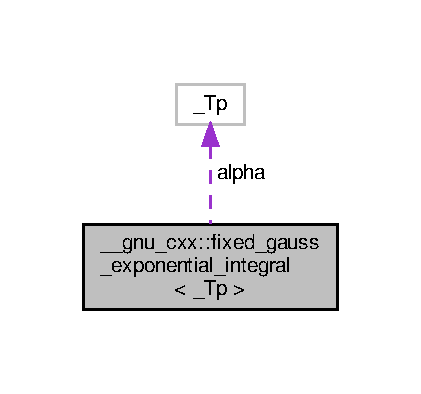
\includegraphics[width=202pt]{struct____gnu__cxx_1_1fixed__gauss__exponential__integral__coll__graph}
\end{center}
\end{figure}
\subsection*{Public Member Functions}
\begin{DoxyCompactItemize}
\item 
\hyperlink{struct____gnu__cxx_1_1fixed__gauss__exponential__integral_a6ea4877ba4237e76210f194531edfa8e}{fixed\+\_\+gauss\+\_\+exponential\+\_\+integral} (int \+\_\+\+\_\+n, \hyperlink{namespace____gnu__cxx_a3b19a9c800ca194374ef9172290f7d79}{\+\_\+\+Tp} \+\_\+\+\_\+alf)
\end{DoxyCompactItemize}
\subsection*{Public Attributes}
\begin{DoxyCompactItemize}
\item 
\hyperlink{namespace____gnu__cxx_a3b19a9c800ca194374ef9172290f7d79}{\+\_\+\+Tp} \hyperlink{struct____gnu__cxx_1_1fixed__gauss__exponential__integral_a44760dd8147de2cdaa7a0817b9f10202}{alpha}
\item 
{\footnotesize template$<$typename \+\_\+\+Func\+Tp $>$ }\\decltype(std\+::invoke\+\_\+result\+\_\+t$<$ \+\_\+\+Func\+Tp, \hyperlink{namespace____gnu__cxx_a3b19a9c800ca194374ef9172290f7d79}{\+\_\+\+Tp} $>$\{\} $\ast$\hyperlink{namespace____gnu__cxx_a3b19a9c800ca194374ef9172290f7d79}{\+\_\+\+Tp}\{\} \hyperlink{struct____gnu__cxx_1_1fixed__gauss__exponential__integral_afe5fe800ebaaf8e6a97034a6c4a17b1e}{operator()} )(\+\_\+\+Func\+Tp \hyperlink{namespace____gnu__cxx_af2b2f0c7a2ae72b922b1afefae5a65b2}{\+\_\+\+\_\+func}, \hyperlink{namespace____gnu__cxx_a3b19a9c800ca194374ef9172290f7d79}{\+\_\+\+Tp} \+\_\+\+\_\+a, \hyperlink{namespace____gnu__cxx_a3b19a9c800ca194374ef9172290f7d79}{\+\_\+\+Tp} \+\_\+\+\_\+b) const
\item 
int \hyperlink{struct____gnu__cxx_1_1fixed__gauss__exponential__integral_a2b72985cb9d78eab9a969e304affcc1c}{order}
\end{DoxyCompactItemize}


\subsection{Detailed Description}
\subsubsection*{template$<$typename \+\_\+\+Tp$>$\newline
struct \+\_\+\+\_\+gnu\+\_\+cxx\+::fixed\+\_\+gauss\+\_\+exponential\+\_\+integral$<$ \+\_\+\+Tp $>$}



Definition at line 213 of file gauss\+\_\+quadrature.\+h.



\subsection{Constructor \& Destructor Documentation}
\mbox{\Hypertarget{struct____gnu__cxx_1_1fixed__gauss__exponential__integral_a6ea4877ba4237e76210f194531edfa8e}\label{struct____gnu__cxx_1_1fixed__gauss__exponential__integral_a6ea4877ba4237e76210f194531edfa8e}} 
\index{\+\_\+\+\_\+gnu\+\_\+cxx\+::fixed\+\_\+gauss\+\_\+exponential\+\_\+integral@{\+\_\+\+\_\+gnu\+\_\+cxx\+::fixed\+\_\+gauss\+\_\+exponential\+\_\+integral}!fixed\+\_\+gauss\+\_\+exponential\+\_\+integral@{fixed\+\_\+gauss\+\_\+exponential\+\_\+integral}}
\index{fixed\+\_\+gauss\+\_\+exponential\+\_\+integral@{fixed\+\_\+gauss\+\_\+exponential\+\_\+integral}!\+\_\+\+\_\+gnu\+\_\+cxx\+::fixed\+\_\+gauss\+\_\+exponential\+\_\+integral@{\+\_\+\+\_\+gnu\+\_\+cxx\+::fixed\+\_\+gauss\+\_\+exponential\+\_\+integral}}
\subsubsection{\texorpdfstring{fixed\+\_\+gauss\+\_\+exponential\+\_\+integral()}{fixed\_gauss\_exponential\_integral()}}
{\footnotesize\ttfamily template$<$typename \+\_\+\+Tp $>$ \\
\hyperlink{struct____gnu__cxx_1_1fixed__gauss__exponential__integral}{\+\_\+\+\_\+gnu\+\_\+cxx\+::fixed\+\_\+gauss\+\_\+exponential\+\_\+integral}$<$ \hyperlink{namespace____gnu__cxx_a3b19a9c800ca194374ef9172290f7d79}{\+\_\+\+Tp} $>$\+::\hyperlink{struct____gnu__cxx_1_1fixed__gauss__exponential__integral}{fixed\+\_\+gauss\+\_\+exponential\+\_\+integral} (\begin{DoxyParamCaption}\item[{int}]{\+\_\+\+\_\+n,  }\item[{\hyperlink{namespace____gnu__cxx_a3b19a9c800ca194374ef9172290f7d79}{\+\_\+\+Tp}}]{\+\_\+\+\_\+alf }\end{DoxyParamCaption})\hspace{0.3cm}{\ttfamily [explicit]}}

Construct a Generalized Gauss-\/\+Exponential rule of order {\ttfamily n}.

Interval\+: $ (a, b) $ Weight function\+: $ |x - (a + b) / 2|^\alpha $ Constraints\+: $ \alpha > -1 $ 

Definition at line 660 of file gauss\+\_\+quadrature.\+tcc.



References \+\_\+\+\_\+gnu\+\_\+cxx\+::\+\_\+\+\_\+func(), \+\_\+\+\_\+gnu\+\_\+cxx\+::\+\_\+\+\_\+detail\+::\+\_\+\+\_\+golub\+\_\+welsch(), \+\_\+\+\_\+gnu\+\_\+cxx\+::\+\_\+\+Ret\+Tp, \+\_\+\+\_\+gnu\+\_\+cxx\+::\+\_\+\+Tp, \+\_\+\+\_\+gnu\+\_\+cxx\+::fixed\+\_\+gauss\+\_\+exponential\+\_\+integral$<$ \+\_\+\+Tp $>$\+::alpha, \+\_\+\+\_\+gnu\+\_\+cxx\+::fixed\+\_\+gauss\+\_\+rational\+\_\+integral$<$ \+\_\+\+Tp $>$\+::fixed\+\_\+gauss\+\_\+rational\+\_\+integral(), and \+\_\+\+\_\+gnu\+\_\+cxx\+::fixed\+\_\+gauss\+\_\+exponential\+\_\+integral$<$ \+\_\+\+Tp $>$\+::order.



Referenced by \+\_\+\+\_\+gnu\+\_\+cxx\+::fixed\+\_\+gauss\+\_\+hermite\+\_\+integral$<$ \+\_\+\+Tp $>$\+::fixed\+\_\+gauss\+\_\+hermite\+\_\+integral().


\begin{DoxyCode}
661     : \hyperlink{struct____gnu__cxx_1_1fixed__gauss__exponential__integral_a2b72985cb9d78eab9a969e304affcc1c}{order}(\_\_n),
662       \hyperlink{struct____gnu__cxx_1_1fixed__gauss__exponential__integral_a44760dd8147de2cdaa7a0817b9f10202}{alpha}(\_\_alf),
663       point(\_\_n),
664       weight(\_\_n)
665     \{
666       \textcolor{keyword}{const} \textcolor{keyword}{auto} \_\_mu\_0 = \hyperlink{namespace____gnu__cxx_a3b19a9c800ca194374ef9172290f7d79}{\_Tp}\{2\} / (this->\hyperlink{struct____gnu__cxx_1_1fixed__gauss__exponential__integral_a44760dd8147de2cdaa7a0817b9f10202}{alpha} + \hyperlink{namespace____gnu__cxx_a3b19a9c800ca194374ef9172290f7d79}{\_Tp}\{1\});
667 
668       std::vector<\_Tp> \_\_diag(this->\hyperlink{struct____gnu__cxx_1_1fixed__gauss__exponential__integral_a2b72985cb9d78eab9a969e304affcc1c}{order}, \hyperlink{namespace____gnu__cxx_a3b19a9c800ca194374ef9172290f7d79}{\_Tp}\{0\});
669       std::vector<\_Tp> \_\_subd(this->\hyperlink{struct____gnu__cxx_1_1fixed__gauss__exponential__integral_a2b72985cb9d78eab9a969e304affcc1c}{order});
670 
671       \textcolor{keyword}{auto} \_\_ap2i = this->\hyperlink{struct____gnu__cxx_1_1fixed__gauss__exponential__integral_a44760dd8147de2cdaa7a0817b9f10202}{alpha};
672       \textcolor{keywordflow}{for} (\textcolor{keywordtype}{int} \_\_i = 1; \_\_i <= this->\hyperlink{struct____gnu__cxx_1_1fixed__gauss__exponential__integral_a2b72985cb9d78eab9a969e304affcc1c}{order}; ++\_\_i)
673         \{
674           \_\_ap2i += \hyperlink{namespace____gnu__cxx_a3b19a9c800ca194374ef9172290f7d79}{\_Tp}\{2\};
675           \_\_subd[\_\_i - 1] = (\hyperlink{namespace____gnu__cxx_a3b19a9c800ca194374ef9172290f7d79}{\_Tp}(\_\_i) + \hyperlink{namespace____gnu__cxx_a3b19a9c800ca194374ef9172290f7d79}{\_Tp}(\_\_i % 2) * this->\hyperlink{struct____gnu__cxx_1_1fixed__gauss__exponential__integral_a44760dd8147de2cdaa7a0817b9f10202}{alpha})
676                           / std::sqrt((\_\_ap2i * \_\_ap2i - \hyperlink{namespace____gnu__cxx_a3b19a9c800ca194374ef9172290f7d79}{\_Tp}\{1\}));
677         \}
678 
679       \hyperlink{namespace____gnu__cxx_1_1____detail_aa9f299bb7c04606a9a9aab3ab9e4f4c8}{\_\_detail::\_\_golub\_welsch}(\_\_mu\_0, this->\hyperlink{struct____gnu__cxx_1_1fixed__gauss__exponential__integral_a2b72985cb9d78eab9a969e304affcc1c}{order}, \_\_diag, \_\_subd,
680                                this->point, this->weight);
681     \}
\end{DoxyCode}


\subsection{Member Data Documentation}
\mbox{\Hypertarget{struct____gnu__cxx_1_1fixed__gauss__exponential__integral_a44760dd8147de2cdaa7a0817b9f10202}\label{struct____gnu__cxx_1_1fixed__gauss__exponential__integral_a44760dd8147de2cdaa7a0817b9f10202}} 
\index{\+\_\+\+\_\+gnu\+\_\+cxx\+::fixed\+\_\+gauss\+\_\+exponential\+\_\+integral@{\+\_\+\+\_\+gnu\+\_\+cxx\+::fixed\+\_\+gauss\+\_\+exponential\+\_\+integral}!alpha@{alpha}}
\index{alpha@{alpha}!\+\_\+\+\_\+gnu\+\_\+cxx\+::fixed\+\_\+gauss\+\_\+exponential\+\_\+integral@{\+\_\+\+\_\+gnu\+\_\+cxx\+::fixed\+\_\+gauss\+\_\+exponential\+\_\+integral}}
\subsubsection{\texorpdfstring{alpha}{alpha}}
{\footnotesize\ttfamily template$<$typename \+\_\+\+Tp$>$ \\
\hyperlink{namespace____gnu__cxx_a3b19a9c800ca194374ef9172290f7d79}{\+\_\+\+Tp} \hyperlink{struct____gnu__cxx_1_1fixed__gauss__exponential__integral}{\+\_\+\+\_\+gnu\+\_\+cxx\+::fixed\+\_\+gauss\+\_\+exponential\+\_\+integral}$<$ \hyperlink{namespace____gnu__cxx_a3b19a9c800ca194374ef9172290f7d79}{\+\_\+\+Tp} $>$\+::alpha}



Definition at line 216 of file gauss\+\_\+quadrature.\+h.



Referenced by \+\_\+\+\_\+gnu\+\_\+cxx\+::fixed\+\_\+gauss\+\_\+exponential\+\_\+integral$<$ \+\_\+\+Tp $>$\+::fixed\+\_\+gauss\+\_\+exponential\+\_\+integral().

\mbox{\Hypertarget{struct____gnu__cxx_1_1fixed__gauss__exponential__integral_afe5fe800ebaaf8e6a97034a6c4a17b1e}\label{struct____gnu__cxx_1_1fixed__gauss__exponential__integral_afe5fe800ebaaf8e6a97034a6c4a17b1e}} 
\index{\+\_\+\+\_\+gnu\+\_\+cxx\+::fixed\+\_\+gauss\+\_\+exponential\+\_\+integral@{\+\_\+\+\_\+gnu\+\_\+cxx\+::fixed\+\_\+gauss\+\_\+exponential\+\_\+integral}!operator()@{operator()}}
\index{operator()@{operator()}!\+\_\+\+\_\+gnu\+\_\+cxx\+::fixed\+\_\+gauss\+\_\+exponential\+\_\+integral@{\+\_\+\+\_\+gnu\+\_\+cxx\+::fixed\+\_\+gauss\+\_\+exponential\+\_\+integral}}
\subsubsection{\texorpdfstring{operator()}{operator()}}
{\footnotesize\ttfamily template$<$typename \+\_\+\+Tp$>$ \\
template$<$typename \+\_\+\+Func\+Tp $>$ \\
decltype(std\+::invoke\+\_\+result\+\_\+t$<$\+\_\+\+Func\+Tp, \hyperlink{namespace____gnu__cxx_a3b19a9c800ca194374ef9172290f7d79}{\+\_\+\+Tp}$>$\{\} $\ast$ \hyperlink{namespace____gnu__cxx_a3b19a9c800ca194374ef9172290f7d79}{\+\_\+\+Tp}\{\} \hyperlink{struct____gnu__cxx_1_1fixed__gauss__exponential__integral}{\+\_\+\+\_\+gnu\+\_\+cxx\+::fixed\+\_\+gauss\+\_\+exponential\+\_\+integral}$<$ \hyperlink{namespace____gnu__cxx_a3b19a9c800ca194374ef9172290f7d79}{\+\_\+\+Tp} $>$\+::operator()) (\+\_\+\+Func\+Tp \hyperlink{namespace____gnu__cxx_af2b2f0c7a2ae72b922b1afefae5a65b2}{\+\_\+\+\_\+func}, \hyperlink{namespace____gnu__cxx_a3b19a9c800ca194374ef9172290f7d79}{\+\_\+\+Tp} \+\_\+\+\_\+a, \hyperlink{namespace____gnu__cxx_a3b19a9c800ca194374ef9172290f7d79}{\+\_\+\+Tp} \+\_\+\+\_\+b) const}



Definition at line 222 of file gauss\+\_\+quadrature.\+h.

\mbox{\Hypertarget{struct____gnu__cxx_1_1fixed__gauss__exponential__integral_a2b72985cb9d78eab9a969e304affcc1c}\label{struct____gnu__cxx_1_1fixed__gauss__exponential__integral_a2b72985cb9d78eab9a969e304affcc1c}} 
\index{\+\_\+\+\_\+gnu\+\_\+cxx\+::fixed\+\_\+gauss\+\_\+exponential\+\_\+integral@{\+\_\+\+\_\+gnu\+\_\+cxx\+::fixed\+\_\+gauss\+\_\+exponential\+\_\+integral}!order@{order}}
\index{order@{order}!\+\_\+\+\_\+gnu\+\_\+cxx\+::fixed\+\_\+gauss\+\_\+exponential\+\_\+integral@{\+\_\+\+\_\+gnu\+\_\+cxx\+::fixed\+\_\+gauss\+\_\+exponential\+\_\+integral}}
\subsubsection{\texorpdfstring{order}{order}}
{\footnotesize\ttfamily template$<$typename \+\_\+\+Tp$>$ \\
int \hyperlink{struct____gnu__cxx_1_1fixed__gauss__exponential__integral}{\+\_\+\+\_\+gnu\+\_\+cxx\+::fixed\+\_\+gauss\+\_\+exponential\+\_\+integral}$<$ \hyperlink{namespace____gnu__cxx_a3b19a9c800ca194374ef9172290f7d79}{\+\_\+\+Tp} $>$\+::order}



Definition at line 215 of file gauss\+\_\+quadrature.\+h.



Referenced by \+\_\+\+\_\+gnu\+\_\+cxx\+::fixed\+\_\+gauss\+\_\+exponential\+\_\+integral$<$ \+\_\+\+Tp $>$\+::fixed\+\_\+gauss\+\_\+exponential\+\_\+integral().



The documentation for this struct was generated from the following files\+:\begin{DoxyCompactItemize}
\item 
include/ext/\hyperlink{gauss__quadrature_8h}{gauss\+\_\+quadrature.\+h}\item 
include/ext/\hyperlink{gauss__quadrature_8tcc}{gauss\+\_\+quadrature.\+tcc}\end{DoxyCompactItemize}

\hypertarget{struct____gnu__cxx_1_1fixed__gauss__gegenbauer__integral}{}\section{\+\_\+\+\_\+gnu\+\_\+cxx\+:\+:fixed\+\_\+gauss\+\_\+gegenbauer\+\_\+integral$<$ \+\_\+\+Tp $>$ Struct Template Reference}
\label{struct____gnu__cxx_1_1fixed__gauss__gegenbauer__integral}\index{\+\_\+\+\_\+gnu\+\_\+cxx\+::fixed\+\_\+gauss\+\_\+gegenbauer\+\_\+integral$<$ \+\_\+\+Tp $>$@{\+\_\+\+\_\+gnu\+\_\+cxx\+::fixed\+\_\+gauss\+\_\+gegenbauer\+\_\+integral$<$ \+\_\+\+Tp $>$}}


{\ttfamily \#include $<$gauss\+\_\+quadrature.\+h$>$}



Collaboration diagram for \+\_\+\+\_\+gnu\+\_\+cxx\+:\+:fixed\+\_\+gauss\+\_\+gegenbauer\+\_\+integral$<$ \+\_\+\+Tp $>$\+:
\nopagebreak
\begin{figure}[H]
\begin{center}
\leavevmode
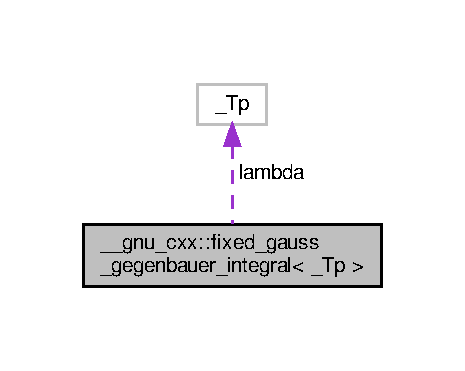
\includegraphics[width=223pt]{struct____gnu__cxx_1_1fixed__gauss__gegenbauer__integral__coll__graph}
\end{center}
\end{figure}
\subsection*{Public Member Functions}
\begin{DoxyCompactItemize}
\item 
\hyperlink{struct____gnu__cxx_1_1fixed__gauss__gegenbauer__integral_a2581f15261fcf06cffd06c99c9cca97e}{fixed\+\_\+gauss\+\_\+gegenbauer\+\_\+integral} (int \+\_\+\+\_\+n, \hyperlink{namespace____gnu__cxx_a3b19a9c800ca194374ef9172290f7d79}{\+\_\+\+Tp} \+\_\+\+\_\+lam)
\end{DoxyCompactItemize}
\subsection*{Public Attributes}
\begin{DoxyCompactItemize}
\item 
\hyperlink{namespace____gnu__cxx_a3b19a9c800ca194374ef9172290f7d79}{\+\_\+\+Tp} \hyperlink{struct____gnu__cxx_1_1fixed__gauss__gegenbauer__integral_a920e1b46f20a45756e3cd563ab7fd1e3}{lambda}
\item 
{\footnotesize template$<$typename \+\_\+\+Func\+Tp $>$ }\\decltype(std\+::invoke\+\_\+result\+\_\+t$<$ \+\_\+\+Func\+Tp, \hyperlink{namespace____gnu__cxx_a3b19a9c800ca194374ef9172290f7d79}{\+\_\+\+Tp} $>$\{\} $\ast$\hyperlink{namespace____gnu__cxx_a3b19a9c800ca194374ef9172290f7d79}{\+\_\+\+Tp}\{\} \hyperlink{struct____gnu__cxx_1_1fixed__gauss__gegenbauer__integral_a16f67fec7b9c704fa11076db362ca938}{operator()} )(\+\_\+\+Func\+Tp \hyperlink{namespace____gnu__cxx_af2b2f0c7a2ae72b922b1afefae5a65b2}{\+\_\+\+\_\+func}, \hyperlink{namespace____gnu__cxx_a3b19a9c800ca194374ef9172290f7d79}{\+\_\+\+Tp} \+\_\+\+\_\+a, \hyperlink{namespace____gnu__cxx_a3b19a9c800ca194374ef9172290f7d79}{\+\_\+\+Tp} \+\_\+\+\_\+b) const
\item 
int \hyperlink{struct____gnu__cxx_1_1fixed__gauss__gegenbauer__integral_ae0cf76d27bf84a9664b8fa94ad1037ea}{order}
\end{DoxyCompactItemize}


\subsection{Detailed Description}
\subsubsection*{template$<$typename \+\_\+\+Tp$>$\newline
struct \+\_\+\+\_\+gnu\+\_\+cxx\+::fixed\+\_\+gauss\+\_\+gegenbauer\+\_\+integral$<$ \+\_\+\+Tp $>$}



Definition at line 132 of file gauss\+\_\+quadrature.\+h.



\subsection{Constructor \& Destructor Documentation}
\mbox{\Hypertarget{struct____gnu__cxx_1_1fixed__gauss__gegenbauer__integral_a2581f15261fcf06cffd06c99c9cca97e}\label{struct____gnu__cxx_1_1fixed__gauss__gegenbauer__integral_a2581f15261fcf06cffd06c99c9cca97e}} 
\index{\+\_\+\+\_\+gnu\+\_\+cxx\+::fixed\+\_\+gauss\+\_\+gegenbauer\+\_\+integral@{\+\_\+\+\_\+gnu\+\_\+cxx\+::fixed\+\_\+gauss\+\_\+gegenbauer\+\_\+integral}!fixed\+\_\+gauss\+\_\+gegenbauer\+\_\+integral@{fixed\+\_\+gauss\+\_\+gegenbauer\+\_\+integral}}
\index{fixed\+\_\+gauss\+\_\+gegenbauer\+\_\+integral@{fixed\+\_\+gauss\+\_\+gegenbauer\+\_\+integral}!\+\_\+\+\_\+gnu\+\_\+cxx\+::fixed\+\_\+gauss\+\_\+gegenbauer\+\_\+integral@{\+\_\+\+\_\+gnu\+\_\+cxx\+::fixed\+\_\+gauss\+\_\+gegenbauer\+\_\+integral}}
\subsubsection{\texorpdfstring{fixed\+\_\+gauss\+\_\+gegenbauer\+\_\+integral()}{fixed\_gauss\_gegenbauer\_integral()}}
{\footnotesize\ttfamily template$<$typename \+\_\+\+Tp $>$ \\
\hyperlink{struct____gnu__cxx_1_1fixed__gauss__gegenbauer__integral}{\+\_\+\+\_\+gnu\+\_\+cxx\+::fixed\+\_\+gauss\+\_\+gegenbauer\+\_\+integral}$<$ \hyperlink{namespace____gnu__cxx_a3b19a9c800ca194374ef9172290f7d79}{\+\_\+\+Tp} $>$\+::\hyperlink{struct____gnu__cxx_1_1fixed__gauss__gegenbauer__integral}{fixed\+\_\+gauss\+\_\+gegenbauer\+\_\+integral} (\begin{DoxyParamCaption}\item[{int}]{\+\_\+\+\_\+n,  }\item[{\hyperlink{namespace____gnu__cxx_a3b19a9c800ca194374ef9172290f7d79}{\+\_\+\+Tp}}]{\+\_\+\+\_\+lam }\end{DoxyParamCaption})\hspace{0.3cm}{\ttfamily [explicit]}}

Construct a Gauss-\/\+Gegenbauer rule of order {\ttfamily n}.

Weight function\+: $ [(b-x)(x-a)]^\lambda $ Constraints\+: $ \lambda > -1 $ 

Definition at line 392 of file gauss\+\_\+quadrature.\+tcc.



References \+\_\+\+\_\+gnu\+\_\+cxx\+::\+\_\+\+\_\+func(), \+\_\+\+\_\+gnu\+\_\+cxx\+::\+\_\+\+\_\+detail\+::\+\_\+\+\_\+golub\+\_\+welsch(), \+\_\+\+\_\+gnu\+\_\+cxx\+::\+\_\+\+Ret\+Tp, \+\_\+\+\_\+gnu\+\_\+cxx\+::\+\_\+\+Tp, \+\_\+\+\_\+gnu\+\_\+cxx\+::fixed\+\_\+gauss\+\_\+jacobi\+\_\+integral$<$ \+\_\+\+Tp $>$\+::fixed\+\_\+gauss\+\_\+jacobi\+\_\+integral(), \+\_\+\+\_\+gnu\+\_\+cxx\+::fixed\+\_\+gauss\+\_\+gegenbauer\+\_\+integral$<$ \+\_\+\+Tp $>$\+::lambda, and \+\_\+\+\_\+gnu\+\_\+cxx\+::fixed\+\_\+gauss\+\_\+gegenbauer\+\_\+integral$<$ \+\_\+\+Tp $>$\+::order.



Referenced by \+\_\+\+\_\+gnu\+\_\+cxx\+::fixed\+\_\+gauss\+\_\+chebyshev\+\_\+w\+\_\+integral$<$ \+\_\+\+Tp $>$\+::fixed\+\_\+gauss\+\_\+chebyshev\+\_\+w\+\_\+integral().


\begin{DoxyCode}
393     : \hyperlink{struct____gnu__cxx_1_1fixed__gauss__gegenbauer__integral_ae0cf76d27bf84a9664b8fa94ad1037ea}{order}(\_\_n),
394       \hyperlink{struct____gnu__cxx_1_1fixed__gauss__gegenbauer__integral_a920e1b46f20a45756e3cd563ab7fd1e3}{lambda}(\_\_lam),
395       point(\_\_n),
396       weight(\_\_n)
397     \{
398       \textcolor{keyword}{const} \textcolor{keyword}{auto} \_\_ab = \hyperlink{namespace____gnu__cxx_a3b19a9c800ca194374ef9172290f7d79}{\_Tp}\{2\} * this->\hyperlink{struct____gnu__cxx_1_1fixed__gauss__gegenbauer__integral_a920e1b46f20a45756e3cd563ab7fd1e3}{lambda};
399       \textcolor{keyword}{const} \textcolor{keyword}{auto} \_\_gam = std::tgamma(this->\hyperlink{struct____gnu__cxx_1_1fixed__gauss__gegenbauer__integral_a920e1b46f20a45756e3cd563ab7fd1e3}{lambda} + \hyperlink{namespace____gnu__cxx_a3b19a9c800ca194374ef9172290f7d79}{\_Tp}\{1\});
400       \textcolor{keyword}{const} \textcolor{keyword}{auto} \_\_mu\_0 = std::pow(\hyperlink{namespace____gnu__cxx_a3b19a9c800ca194374ef9172290f7d79}{\_Tp}\{2\}, \_\_ab + \hyperlink{namespace____gnu__cxx_a3b19a9c800ca194374ef9172290f7d79}{\_Tp}\{1\})
401                         * \_\_gam * \_\_gam / std::tgamma(\_\_ab + \hyperlink{namespace____gnu__cxx_a3b19a9c800ca194374ef9172290f7d79}{\_Tp}\{2\});
402 
403       std::vector<\_Tp> \_\_diag(this->\hyperlink{struct____gnu__cxx_1_1fixed__gauss__gegenbauer__integral_ae0cf76d27bf84a9664b8fa94ad1037ea}{order}, \hyperlink{namespace____gnu__cxx_a3b19a9c800ca194374ef9172290f7d79}{\_Tp}\{0\});
404       std::vector<\_Tp> \_\_subd(this->\hyperlink{struct____gnu__cxx_1_1fixed__gauss__gegenbauer__integral_ae0cf76d27bf84a9664b8fa94ad1037ea}{order});
405 
406       \_\_subd[0] = std::sqrt(\hyperlink{namespace____gnu__cxx_a3b19a9c800ca194374ef9172290f7d79}{\_Tp}\{1\} / (\hyperlink{namespace____gnu__cxx_a3b19a9c800ca194374ef9172290f7d79}{\_Tp}\{2\} * this->\hyperlink{struct____gnu__cxx_1_1fixed__gauss__gegenbauer__integral_a920e1b46f20a45756e3cd563ab7fd1e3}{lambda} + \hyperlink{namespace____gnu__cxx_a3b19a9c800ca194374ef9172290f7d79}{\_Tp}\{3\}));
407 
408       \textcolor{keywordflow}{for} (\textcolor{keywordtype}{int} \_\_i = 2; \_\_i <= this->\hyperlink{struct____gnu__cxx_1_1fixed__gauss__gegenbauer__integral_ae0cf76d27bf84a9664b8fa94ad1037ea}{order}; ++\_\_i)
409         \_\_subd[\_\_i - 1] = std::sqrt(\hyperlink{namespace____gnu__cxx_a3b19a9c800ca194374ef9172290f7d79}{\_Tp}(\_\_i) * (\_\_ab + \hyperlink{namespace____gnu__cxx_a3b19a9c800ca194374ef9172290f7d79}{\_Tp}(\_\_i))
410                         / (\hyperlink{namespace____gnu__cxx_a3b19a9c800ca194374ef9172290f7d79}{\_Tp}\{4\}
411                           * std::pow(this->\hyperlink{struct____gnu__cxx_1_1fixed__gauss__gegenbauer__integral_a920e1b46f20a45756e3cd563ab7fd1e3}{lambda} + \hyperlink{namespace____gnu__cxx_a3b19a9c800ca194374ef9172290f7d79}{\_Tp}(\_\_i), \hyperlink{namespace____gnu__cxx_a3b19a9c800ca194374ef9172290f7d79}{\_Tp}\{2\}) - 
      \hyperlink{namespace____gnu__cxx_a3b19a9c800ca194374ef9172290f7d79}{\_Tp}\{1\}));
412 
413       \hyperlink{namespace____gnu__cxx_1_1____detail_aa9f299bb7c04606a9a9aab3ab9e4f4c8}{\_\_detail::\_\_golub\_welsch}(\_\_mu\_0, this->\hyperlink{struct____gnu__cxx_1_1fixed__gauss__gegenbauer__integral_ae0cf76d27bf84a9664b8fa94ad1037ea}{order}, \_\_diag, \_\_subd,
414                                this->point, this->weight);
415     \}
\end{DoxyCode}


\subsection{Member Data Documentation}
\mbox{\Hypertarget{struct____gnu__cxx_1_1fixed__gauss__gegenbauer__integral_a920e1b46f20a45756e3cd563ab7fd1e3}\label{struct____gnu__cxx_1_1fixed__gauss__gegenbauer__integral_a920e1b46f20a45756e3cd563ab7fd1e3}} 
\index{\+\_\+\+\_\+gnu\+\_\+cxx\+::fixed\+\_\+gauss\+\_\+gegenbauer\+\_\+integral@{\+\_\+\+\_\+gnu\+\_\+cxx\+::fixed\+\_\+gauss\+\_\+gegenbauer\+\_\+integral}!lambda@{lambda}}
\index{lambda@{lambda}!\+\_\+\+\_\+gnu\+\_\+cxx\+::fixed\+\_\+gauss\+\_\+gegenbauer\+\_\+integral@{\+\_\+\+\_\+gnu\+\_\+cxx\+::fixed\+\_\+gauss\+\_\+gegenbauer\+\_\+integral}}
\subsubsection{\texorpdfstring{lambda}{lambda}}
{\footnotesize\ttfamily template$<$typename \+\_\+\+Tp$>$ \\
\hyperlink{namespace____gnu__cxx_a3b19a9c800ca194374ef9172290f7d79}{\+\_\+\+Tp} \hyperlink{struct____gnu__cxx_1_1fixed__gauss__gegenbauer__integral}{\+\_\+\+\_\+gnu\+\_\+cxx\+::fixed\+\_\+gauss\+\_\+gegenbauer\+\_\+integral}$<$ \hyperlink{namespace____gnu__cxx_a3b19a9c800ca194374ef9172290f7d79}{\+\_\+\+Tp} $>$\+::lambda}



Definition at line 135 of file gauss\+\_\+quadrature.\+h.



Referenced by \+\_\+\+\_\+gnu\+\_\+cxx\+::fixed\+\_\+gauss\+\_\+gegenbauer\+\_\+integral$<$ \+\_\+\+Tp $>$\+::fixed\+\_\+gauss\+\_\+gegenbauer\+\_\+integral().

\mbox{\Hypertarget{struct____gnu__cxx_1_1fixed__gauss__gegenbauer__integral_a16f67fec7b9c704fa11076db362ca938}\label{struct____gnu__cxx_1_1fixed__gauss__gegenbauer__integral_a16f67fec7b9c704fa11076db362ca938}} 
\index{\+\_\+\+\_\+gnu\+\_\+cxx\+::fixed\+\_\+gauss\+\_\+gegenbauer\+\_\+integral@{\+\_\+\+\_\+gnu\+\_\+cxx\+::fixed\+\_\+gauss\+\_\+gegenbauer\+\_\+integral}!operator()@{operator()}}
\index{operator()@{operator()}!\+\_\+\+\_\+gnu\+\_\+cxx\+::fixed\+\_\+gauss\+\_\+gegenbauer\+\_\+integral@{\+\_\+\+\_\+gnu\+\_\+cxx\+::fixed\+\_\+gauss\+\_\+gegenbauer\+\_\+integral}}
\subsubsection{\texorpdfstring{operator()}{operator()}}
{\footnotesize\ttfamily template$<$typename \+\_\+\+Tp$>$ \\
template$<$typename \+\_\+\+Func\+Tp $>$ \\
decltype(std\+::invoke\+\_\+result\+\_\+t$<$\+\_\+\+Func\+Tp, \hyperlink{namespace____gnu__cxx_a3b19a9c800ca194374ef9172290f7d79}{\+\_\+\+Tp}$>$\{\} $\ast$ \hyperlink{namespace____gnu__cxx_a3b19a9c800ca194374ef9172290f7d79}{\+\_\+\+Tp}\{\} \hyperlink{struct____gnu__cxx_1_1fixed__gauss__gegenbauer__integral}{\+\_\+\+\_\+gnu\+\_\+cxx\+::fixed\+\_\+gauss\+\_\+gegenbauer\+\_\+integral}$<$ \hyperlink{namespace____gnu__cxx_a3b19a9c800ca194374ef9172290f7d79}{\+\_\+\+Tp} $>$\+::operator()) (\+\_\+\+Func\+Tp \hyperlink{namespace____gnu__cxx_af2b2f0c7a2ae72b922b1afefae5a65b2}{\+\_\+\+\_\+func}, \hyperlink{namespace____gnu__cxx_a3b19a9c800ca194374ef9172290f7d79}{\+\_\+\+Tp} \+\_\+\+\_\+a, \hyperlink{namespace____gnu__cxx_a3b19a9c800ca194374ef9172290f7d79}{\+\_\+\+Tp} \+\_\+\+\_\+b) const}



Definition at line 141 of file gauss\+\_\+quadrature.\+h.

\mbox{\Hypertarget{struct____gnu__cxx_1_1fixed__gauss__gegenbauer__integral_ae0cf76d27bf84a9664b8fa94ad1037ea}\label{struct____gnu__cxx_1_1fixed__gauss__gegenbauer__integral_ae0cf76d27bf84a9664b8fa94ad1037ea}} 
\index{\+\_\+\+\_\+gnu\+\_\+cxx\+::fixed\+\_\+gauss\+\_\+gegenbauer\+\_\+integral@{\+\_\+\+\_\+gnu\+\_\+cxx\+::fixed\+\_\+gauss\+\_\+gegenbauer\+\_\+integral}!order@{order}}
\index{order@{order}!\+\_\+\+\_\+gnu\+\_\+cxx\+::fixed\+\_\+gauss\+\_\+gegenbauer\+\_\+integral@{\+\_\+\+\_\+gnu\+\_\+cxx\+::fixed\+\_\+gauss\+\_\+gegenbauer\+\_\+integral}}
\subsubsection{\texorpdfstring{order}{order}}
{\footnotesize\ttfamily template$<$typename \+\_\+\+Tp$>$ \\
int \hyperlink{struct____gnu__cxx_1_1fixed__gauss__gegenbauer__integral}{\+\_\+\+\_\+gnu\+\_\+cxx\+::fixed\+\_\+gauss\+\_\+gegenbauer\+\_\+integral}$<$ \hyperlink{namespace____gnu__cxx_a3b19a9c800ca194374ef9172290f7d79}{\+\_\+\+Tp} $>$\+::order}



Definition at line 134 of file gauss\+\_\+quadrature.\+h.



Referenced by \+\_\+\+\_\+gnu\+\_\+cxx\+::fixed\+\_\+gauss\+\_\+gegenbauer\+\_\+integral$<$ \+\_\+\+Tp $>$\+::fixed\+\_\+gauss\+\_\+gegenbauer\+\_\+integral().



The documentation for this struct was generated from the following files\+:\begin{DoxyCompactItemize}
\item 
include/ext/\hyperlink{gauss__quadrature_8h}{gauss\+\_\+quadrature.\+h}\item 
include/ext/\hyperlink{gauss__quadrature_8tcc}{gauss\+\_\+quadrature.\+tcc}\end{DoxyCompactItemize}

\hypertarget{struct____gnu__cxx_1_1fixed__gauss__hermite__integral}{}\section{\+\_\+\+\_\+gnu\+\_\+cxx\+:\+:fixed\+\_\+gauss\+\_\+hermite\+\_\+integral$<$ \+\_\+\+Tp $>$ Struct Template Reference}
\label{struct____gnu__cxx_1_1fixed__gauss__hermite__integral}\index{\+\_\+\+\_\+gnu\+\_\+cxx\+::fixed\+\_\+gauss\+\_\+hermite\+\_\+integral$<$ \+\_\+\+Tp $>$@{\+\_\+\+\_\+gnu\+\_\+cxx\+::fixed\+\_\+gauss\+\_\+hermite\+\_\+integral$<$ \+\_\+\+Tp $>$}}


{\ttfamily \#include $<$gauss\+\_\+quadrature.\+h$>$}



Collaboration diagram for \+\_\+\+\_\+gnu\+\_\+cxx\+:\+:fixed\+\_\+gauss\+\_\+hermite\+\_\+integral$<$ \+\_\+\+Tp $>$\+:
\nopagebreak
\begin{figure}[H]
\begin{center}
\leavevmode
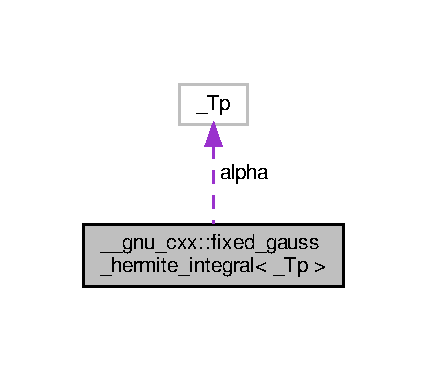
\includegraphics[width=205pt]{struct____gnu__cxx_1_1fixed__gauss__hermite__integral__coll__graph}
\end{center}
\end{figure}
\subsection*{Public Member Functions}
\begin{DoxyCompactItemize}
\item 
\hyperlink{struct____gnu__cxx_1_1fixed__gauss__hermite__integral_afb6f594f7724e05c648326005e4302a7}{fixed\+\_\+gauss\+\_\+hermite\+\_\+integral} (int \+\_\+\+\_\+n, \hyperlink{namespace____gnu__cxx_a3b19a9c800ca194374ef9172290f7d79}{\+\_\+\+Tp} \+\_\+\+\_\+alf)
\end{DoxyCompactItemize}
\subsection*{Public Attributes}
\begin{DoxyCompactItemize}
\item 
\hyperlink{namespace____gnu__cxx_a3b19a9c800ca194374ef9172290f7d79}{\+\_\+\+Tp} \hyperlink{struct____gnu__cxx_1_1fixed__gauss__hermite__integral_a2e8e1a2af7c80ed56beba1a49d222c2e}{alpha}
\item 
{\footnotesize template$<$typename \+\_\+\+Func\+Tp $>$ }\\decltype(std\+::invoke\+\_\+result\+\_\+t$<$ \+\_\+\+Func\+Tp, \hyperlink{namespace____gnu__cxx_a3b19a9c800ca194374ef9172290f7d79}{\+\_\+\+Tp} $>$\{\} $\ast$\hyperlink{namespace____gnu__cxx_a3b19a9c800ca194374ef9172290f7d79}{\+\_\+\+Tp}\{\} \hyperlink{struct____gnu__cxx_1_1fixed__gauss__hermite__integral_a9d7212ceef93046f59568b551e9eef1e}{operator()} )(\+\_\+\+Func\+Tp \hyperlink{namespace____gnu__cxx_af2b2f0c7a2ae72b922b1afefae5a65b2}{\+\_\+\+\_\+func}, \hyperlink{namespace____gnu__cxx_a3b19a9c800ca194374ef9172290f7d79}{\+\_\+\+Tp} \+\_\+\+\_\+a, \hyperlink{namespace____gnu__cxx_a3b19a9c800ca194374ef9172290f7d79}{\+\_\+\+Tp} \+\_\+\+\_\+b) const
\item 
int \hyperlink{struct____gnu__cxx_1_1fixed__gauss__hermite__integral_ad2678dce9fba6604be4d2839c6bc7646}{order}
\end{DoxyCompactItemize}


\subsection{Detailed Description}
\subsubsection*{template$<$typename \+\_\+\+Tp$>$\newline
struct \+\_\+\+\_\+gnu\+\_\+cxx\+::fixed\+\_\+gauss\+\_\+hermite\+\_\+integral$<$ \+\_\+\+Tp $>$}



Definition at line 193 of file gauss\+\_\+quadrature.\+h.



\subsection{Constructor \& Destructor Documentation}
\mbox{\Hypertarget{struct____gnu__cxx_1_1fixed__gauss__hermite__integral_afb6f594f7724e05c648326005e4302a7}\label{struct____gnu__cxx_1_1fixed__gauss__hermite__integral_afb6f594f7724e05c648326005e4302a7}} 
\index{\+\_\+\+\_\+gnu\+\_\+cxx\+::fixed\+\_\+gauss\+\_\+hermite\+\_\+integral@{\+\_\+\+\_\+gnu\+\_\+cxx\+::fixed\+\_\+gauss\+\_\+hermite\+\_\+integral}!fixed\+\_\+gauss\+\_\+hermite\+\_\+integral@{fixed\+\_\+gauss\+\_\+hermite\+\_\+integral}}
\index{fixed\+\_\+gauss\+\_\+hermite\+\_\+integral@{fixed\+\_\+gauss\+\_\+hermite\+\_\+integral}!\+\_\+\+\_\+gnu\+\_\+cxx\+::fixed\+\_\+gauss\+\_\+hermite\+\_\+integral@{\+\_\+\+\_\+gnu\+\_\+cxx\+::fixed\+\_\+gauss\+\_\+hermite\+\_\+integral}}
\subsubsection{\texorpdfstring{fixed\+\_\+gauss\+\_\+hermite\+\_\+integral()}{fixed\_gauss\_hermite\_integral()}}
{\footnotesize\ttfamily template$<$typename \+\_\+\+Tp $>$ \\
\hyperlink{struct____gnu__cxx_1_1fixed__gauss__hermite__integral}{\+\_\+\+\_\+gnu\+\_\+cxx\+::fixed\+\_\+gauss\+\_\+hermite\+\_\+integral}$<$ \hyperlink{namespace____gnu__cxx_a3b19a9c800ca194374ef9172290f7d79}{\+\_\+\+Tp} $>$\+::\hyperlink{struct____gnu__cxx_1_1fixed__gauss__hermite__integral}{fixed\+\_\+gauss\+\_\+hermite\+\_\+integral} (\begin{DoxyParamCaption}\item[{int}]{\+\_\+\+\_\+n,  }\item[{\hyperlink{namespace____gnu__cxx_a3b19a9c800ca194374ef9172290f7d79}{\+\_\+\+Tp}}]{\+\_\+\+\_\+alf }\end{DoxyParamCaption})\hspace{0.3cm}{\ttfamily [explicit]}}

Construct a Generalized Gauss-\/\+Hermite rule of order {\ttfamily n}.

Interval\+: $ (-\infty, \infty) $ Weight function\+: $ |x-a|^\alpha \exp(-b(x-a)^2) $ Constraints\+: $ \alpha > -1 $ 

Definition at line 603 of file gauss\+\_\+quadrature.\+tcc.



References \+\_\+\+\_\+gnu\+\_\+cxx\+::\+\_\+\+\_\+func(), \+\_\+\+\_\+gnu\+\_\+cxx\+::\+\_\+\+\_\+detail\+::\+\_\+\+\_\+golub\+\_\+welsch(), \+\_\+\+\_\+gnu\+\_\+cxx\+::\+\_\+\+Ret\+Tp, \+\_\+\+\_\+gnu\+\_\+cxx\+::\+\_\+\+Tp, \+\_\+\+\_\+gnu\+\_\+cxx\+::fixed\+\_\+gauss\+\_\+hermite\+\_\+integral$<$ \+\_\+\+Tp $>$\+::alpha, \+\_\+\+\_\+gnu\+\_\+cxx\+::fixed\+\_\+gauss\+\_\+exponential\+\_\+integral$<$ \+\_\+\+Tp $>$\+::fixed\+\_\+gauss\+\_\+exponential\+\_\+integral(), and \+\_\+\+\_\+gnu\+\_\+cxx\+::fixed\+\_\+gauss\+\_\+hermite\+\_\+integral$<$ \+\_\+\+Tp $>$\+::order.



Referenced by \+\_\+\+\_\+gnu\+\_\+cxx\+::fixed\+\_\+gauss\+\_\+laguerre\+\_\+integral$<$ \+\_\+\+Tp $>$\+::fixed\+\_\+gauss\+\_\+laguerre\+\_\+integral().


\begin{DoxyCode}
604     : \hyperlink{struct____gnu__cxx_1_1fixed__gauss__hermite__integral_ad2678dce9fba6604be4d2839c6bc7646}{order}(\_\_n),
605       \hyperlink{struct____gnu__cxx_1_1fixed__gauss__hermite__integral_a2e8e1a2af7c80ed56beba1a49d222c2e}{alpha}(\_\_alf),
606       point(\_\_n),
607       weight(\_\_n)
608     \{
609       \textcolor{keyword}{const} \textcolor{keyword}{auto} \_\_mu\_0 = std::tgamma((this->\hyperlink{struct____gnu__cxx_1_1fixed__gauss__hermite__integral_a2e8e1a2af7c80ed56beba1a49d222c2e}{alpha} + \hyperlink{namespace____gnu__cxx_a3b19a9c800ca194374ef9172290f7d79}{\_Tp}\{1\}) / \hyperlink{namespace____gnu__cxx_a3b19a9c800ca194374ef9172290f7d79}{\_Tp}\{2\});
610 
611       std::vector<\_Tp> \_\_diag(this->\hyperlink{struct____gnu__cxx_1_1fixed__gauss__hermite__integral_ad2678dce9fba6604be4d2839c6bc7646}{order}, \hyperlink{namespace____gnu__cxx_a3b19a9c800ca194374ef9172290f7d79}{\_Tp}\{0\});
612       std::vector<\_Tp> \_\_subd(this->\hyperlink{struct____gnu__cxx_1_1fixed__gauss__hermite__integral_ad2678dce9fba6604be4d2839c6bc7646}{order});
613 
614       \textcolor{keywordflow}{for} (\textcolor{keywordtype}{int} \_\_i = 1; \_\_i <= this->\hyperlink{struct____gnu__cxx_1_1fixed__gauss__hermite__integral_ad2678dce9fba6604be4d2839c6bc7646}{order}; ++\_\_i)
615         \_\_subd[\_\_i - 1] = std::sqrt((\hyperlink{namespace____gnu__cxx_a3b19a9c800ca194374ef9172290f7d79}{\_Tp}(\_\_i) + \hyperlink{namespace____gnu__cxx_a3b19a9c800ca194374ef9172290f7d79}{\_Tp}(\_\_i % 2) * this->\hyperlink{struct____gnu__cxx_1_1fixed__gauss__hermite__integral_a2e8e1a2af7c80ed56beba1a49d222c2e}{alpha})
616                                    / \hyperlink{namespace____gnu__cxx_a3b19a9c800ca194374ef9172290f7d79}{\_Tp}\{2\});
617 
618       \hyperlink{namespace____gnu__cxx_1_1____detail_aa9f299bb7c04606a9a9aab3ab9e4f4c8}{\_\_detail::\_\_golub\_welsch}(\_\_mu\_0, this->\hyperlink{struct____gnu__cxx_1_1fixed__gauss__hermite__integral_ad2678dce9fba6604be4d2839c6bc7646}{order}, \_\_diag, \_\_subd,
619                                this->point, this->weight);
620     \}
\end{DoxyCode}


\subsection{Member Data Documentation}
\mbox{\Hypertarget{struct____gnu__cxx_1_1fixed__gauss__hermite__integral_a2e8e1a2af7c80ed56beba1a49d222c2e}\label{struct____gnu__cxx_1_1fixed__gauss__hermite__integral_a2e8e1a2af7c80ed56beba1a49d222c2e}} 
\index{\+\_\+\+\_\+gnu\+\_\+cxx\+::fixed\+\_\+gauss\+\_\+hermite\+\_\+integral@{\+\_\+\+\_\+gnu\+\_\+cxx\+::fixed\+\_\+gauss\+\_\+hermite\+\_\+integral}!alpha@{alpha}}
\index{alpha@{alpha}!\+\_\+\+\_\+gnu\+\_\+cxx\+::fixed\+\_\+gauss\+\_\+hermite\+\_\+integral@{\+\_\+\+\_\+gnu\+\_\+cxx\+::fixed\+\_\+gauss\+\_\+hermite\+\_\+integral}}
\subsubsection{\texorpdfstring{alpha}{alpha}}
{\footnotesize\ttfamily template$<$typename \+\_\+\+Tp$>$ \\
\hyperlink{namespace____gnu__cxx_a3b19a9c800ca194374ef9172290f7d79}{\+\_\+\+Tp} \hyperlink{struct____gnu__cxx_1_1fixed__gauss__hermite__integral}{\+\_\+\+\_\+gnu\+\_\+cxx\+::fixed\+\_\+gauss\+\_\+hermite\+\_\+integral}$<$ \hyperlink{namespace____gnu__cxx_a3b19a9c800ca194374ef9172290f7d79}{\+\_\+\+Tp} $>$\+::alpha}



Definition at line 196 of file gauss\+\_\+quadrature.\+h.



Referenced by \+\_\+\+\_\+gnu\+\_\+cxx\+::fixed\+\_\+gauss\+\_\+hermite\+\_\+integral$<$ \+\_\+\+Tp $>$\+::fixed\+\_\+gauss\+\_\+hermite\+\_\+integral().

\mbox{\Hypertarget{struct____gnu__cxx_1_1fixed__gauss__hermite__integral_a9d7212ceef93046f59568b551e9eef1e}\label{struct____gnu__cxx_1_1fixed__gauss__hermite__integral_a9d7212ceef93046f59568b551e9eef1e}} 
\index{\+\_\+\+\_\+gnu\+\_\+cxx\+::fixed\+\_\+gauss\+\_\+hermite\+\_\+integral@{\+\_\+\+\_\+gnu\+\_\+cxx\+::fixed\+\_\+gauss\+\_\+hermite\+\_\+integral}!operator()@{operator()}}
\index{operator()@{operator()}!\+\_\+\+\_\+gnu\+\_\+cxx\+::fixed\+\_\+gauss\+\_\+hermite\+\_\+integral@{\+\_\+\+\_\+gnu\+\_\+cxx\+::fixed\+\_\+gauss\+\_\+hermite\+\_\+integral}}
\subsubsection{\texorpdfstring{operator()}{operator()}}
{\footnotesize\ttfamily template$<$typename \+\_\+\+Tp$>$ \\
template$<$typename \+\_\+\+Func\+Tp $>$ \\
decltype(std\+::invoke\+\_\+result\+\_\+t$<$\+\_\+\+Func\+Tp, \hyperlink{namespace____gnu__cxx_a3b19a9c800ca194374ef9172290f7d79}{\+\_\+\+Tp}$>$\{\} $\ast$ \hyperlink{namespace____gnu__cxx_a3b19a9c800ca194374ef9172290f7d79}{\+\_\+\+Tp}\{\} \hyperlink{struct____gnu__cxx_1_1fixed__gauss__hermite__integral}{\+\_\+\+\_\+gnu\+\_\+cxx\+::fixed\+\_\+gauss\+\_\+hermite\+\_\+integral}$<$ \hyperlink{namespace____gnu__cxx_a3b19a9c800ca194374ef9172290f7d79}{\+\_\+\+Tp} $>$\+::operator()) (\+\_\+\+Func\+Tp \hyperlink{namespace____gnu__cxx_af2b2f0c7a2ae72b922b1afefae5a65b2}{\+\_\+\+\_\+func}, \hyperlink{namespace____gnu__cxx_a3b19a9c800ca194374ef9172290f7d79}{\+\_\+\+Tp} \+\_\+\+\_\+a, \hyperlink{namespace____gnu__cxx_a3b19a9c800ca194374ef9172290f7d79}{\+\_\+\+Tp} \+\_\+\+\_\+b) const}



Definition at line 202 of file gauss\+\_\+quadrature.\+h.

\mbox{\Hypertarget{struct____gnu__cxx_1_1fixed__gauss__hermite__integral_ad2678dce9fba6604be4d2839c6bc7646}\label{struct____gnu__cxx_1_1fixed__gauss__hermite__integral_ad2678dce9fba6604be4d2839c6bc7646}} 
\index{\+\_\+\+\_\+gnu\+\_\+cxx\+::fixed\+\_\+gauss\+\_\+hermite\+\_\+integral@{\+\_\+\+\_\+gnu\+\_\+cxx\+::fixed\+\_\+gauss\+\_\+hermite\+\_\+integral}!order@{order}}
\index{order@{order}!\+\_\+\+\_\+gnu\+\_\+cxx\+::fixed\+\_\+gauss\+\_\+hermite\+\_\+integral@{\+\_\+\+\_\+gnu\+\_\+cxx\+::fixed\+\_\+gauss\+\_\+hermite\+\_\+integral}}
\subsubsection{\texorpdfstring{order}{order}}
{\footnotesize\ttfamily template$<$typename \+\_\+\+Tp$>$ \\
int \hyperlink{struct____gnu__cxx_1_1fixed__gauss__hermite__integral}{\+\_\+\+\_\+gnu\+\_\+cxx\+::fixed\+\_\+gauss\+\_\+hermite\+\_\+integral}$<$ \hyperlink{namespace____gnu__cxx_a3b19a9c800ca194374ef9172290f7d79}{\+\_\+\+Tp} $>$\+::order}



Definition at line 195 of file gauss\+\_\+quadrature.\+h.



Referenced by \+\_\+\+\_\+gnu\+\_\+cxx\+::fixed\+\_\+gauss\+\_\+hermite\+\_\+integral$<$ \+\_\+\+Tp $>$\+::fixed\+\_\+gauss\+\_\+hermite\+\_\+integral().



The documentation for this struct was generated from the following files\+:\begin{DoxyCompactItemize}
\item 
include/ext/\hyperlink{gauss__quadrature_8h}{gauss\+\_\+quadrature.\+h}\item 
include/ext/\hyperlink{gauss__quadrature_8tcc}{gauss\+\_\+quadrature.\+tcc}\end{DoxyCompactItemize}

\hypertarget{struct____gnu__cxx_1_1fixed__gauss__jacobi__integral}{}\section{\+\_\+\+\_\+gnu\+\_\+cxx\+:\+:fixed\+\_\+gauss\+\_\+jacobi\+\_\+integral$<$ \+\_\+\+Tp $>$ Struct Template Reference}
\label{struct____gnu__cxx_1_1fixed__gauss__jacobi__integral}\index{\+\_\+\+\_\+gnu\+\_\+cxx\+::fixed\+\_\+gauss\+\_\+jacobi\+\_\+integral$<$ \+\_\+\+Tp $>$@{\+\_\+\+\_\+gnu\+\_\+cxx\+::fixed\+\_\+gauss\+\_\+jacobi\+\_\+integral$<$ \+\_\+\+Tp $>$}}


{\ttfamily \#include $<$gauss\+\_\+quadrature.\+h$>$}



Collaboration diagram for \+\_\+\+\_\+gnu\+\_\+cxx\+:\+:fixed\+\_\+gauss\+\_\+jacobi\+\_\+integral$<$ \+\_\+\+Tp $>$\+:
\nopagebreak
\begin{figure}[H]
\begin{center}
\leavevmode
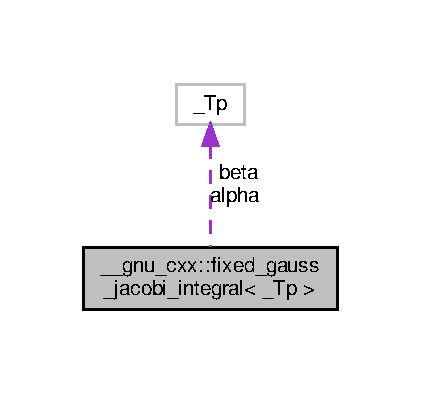
\includegraphics[width=202pt]{struct____gnu__cxx_1_1fixed__gauss__jacobi__integral__coll__graph}
\end{center}
\end{figure}
\subsection*{Public Member Functions}
\begin{DoxyCompactItemize}
\item 
\hyperlink{struct____gnu__cxx_1_1fixed__gauss__jacobi__integral_a2ee234de6447ed621c4199beb169126b}{fixed\+\_\+gauss\+\_\+jacobi\+\_\+integral} (int \+\_\+\+\_\+n, \hyperlink{namespace____gnu__cxx_a3b19a9c800ca194374ef9172290f7d79}{\+\_\+\+Tp} \+\_\+\+\_\+alf, \hyperlink{namespace____gnu__cxx_a3b19a9c800ca194374ef9172290f7d79}{\+\_\+\+Tp} \+\_\+\+\_\+bet)
\end{DoxyCompactItemize}
\subsection*{Public Attributes}
\begin{DoxyCompactItemize}
\item 
\hyperlink{namespace____gnu__cxx_a3b19a9c800ca194374ef9172290f7d79}{\+\_\+\+Tp} \hyperlink{struct____gnu__cxx_1_1fixed__gauss__jacobi__integral_a2d9b81150e8fed046b6753551e9ce0e1}{alpha}
\item 
\hyperlink{namespace____gnu__cxx_a3b19a9c800ca194374ef9172290f7d79}{\+\_\+\+Tp} \hyperlink{struct____gnu__cxx_1_1fixed__gauss__jacobi__integral_aa9e160852c8912532deda29fae96824a}{beta}
\item 
{\footnotesize template$<$typename \+\_\+\+Func\+Tp $>$ }\\decltype(std\+::invoke\+\_\+result\+\_\+t$<$ \+\_\+\+Func\+Tp, \hyperlink{namespace____gnu__cxx_a3b19a9c800ca194374ef9172290f7d79}{\+\_\+\+Tp} $>$\{\} $\ast$\hyperlink{namespace____gnu__cxx_a3b19a9c800ca194374ef9172290f7d79}{\+\_\+\+Tp}\{\} \hyperlink{struct____gnu__cxx_1_1fixed__gauss__jacobi__integral_ad20389e68e1c98098f892b118e614498}{operator()} )(\+\_\+\+Func\+Tp \hyperlink{namespace____gnu__cxx_af2b2f0c7a2ae72b922b1afefae5a65b2}{\+\_\+\+\_\+func}, \hyperlink{namespace____gnu__cxx_a3b19a9c800ca194374ef9172290f7d79}{\+\_\+\+Tp} \+\_\+\+\_\+a, \hyperlink{namespace____gnu__cxx_a3b19a9c800ca194374ef9172290f7d79}{\+\_\+\+Tp} \+\_\+\+\_\+b) const
\item 
int \hyperlink{struct____gnu__cxx_1_1fixed__gauss__jacobi__integral_ae5f494962a95203a0f799f039e4b6b33}{order}
\end{DoxyCompactItemize}


\subsection{Detailed Description}
\subsubsection*{template$<$typename \+\_\+\+Tp$>$\newline
struct \+\_\+\+\_\+gnu\+\_\+cxx\+::fixed\+\_\+gauss\+\_\+jacobi\+\_\+integral$<$ \+\_\+\+Tp $>$}



Definition at line 152 of file gauss\+\_\+quadrature.\+h.



\subsection{Constructor \& Destructor Documentation}
\mbox{\Hypertarget{struct____gnu__cxx_1_1fixed__gauss__jacobi__integral_a2ee234de6447ed621c4199beb169126b}\label{struct____gnu__cxx_1_1fixed__gauss__jacobi__integral_a2ee234de6447ed621c4199beb169126b}} 
\index{\+\_\+\+\_\+gnu\+\_\+cxx\+::fixed\+\_\+gauss\+\_\+jacobi\+\_\+integral@{\+\_\+\+\_\+gnu\+\_\+cxx\+::fixed\+\_\+gauss\+\_\+jacobi\+\_\+integral}!fixed\+\_\+gauss\+\_\+jacobi\+\_\+integral@{fixed\+\_\+gauss\+\_\+jacobi\+\_\+integral}}
\index{fixed\+\_\+gauss\+\_\+jacobi\+\_\+integral@{fixed\+\_\+gauss\+\_\+jacobi\+\_\+integral}!\+\_\+\+\_\+gnu\+\_\+cxx\+::fixed\+\_\+gauss\+\_\+jacobi\+\_\+integral@{\+\_\+\+\_\+gnu\+\_\+cxx\+::fixed\+\_\+gauss\+\_\+jacobi\+\_\+integral}}
\subsubsection{\texorpdfstring{fixed\+\_\+gauss\+\_\+jacobi\+\_\+integral()}{fixed\_gauss\_jacobi\_integral()}}
{\footnotesize\ttfamily template$<$typename \+\_\+\+Tp $>$ \\
\hyperlink{struct____gnu__cxx_1_1fixed__gauss__jacobi__integral}{\+\_\+\+\_\+gnu\+\_\+cxx\+::fixed\+\_\+gauss\+\_\+jacobi\+\_\+integral}$<$ \hyperlink{namespace____gnu__cxx_a3b19a9c800ca194374ef9172290f7d79}{\+\_\+\+Tp} $>$\+::\hyperlink{struct____gnu__cxx_1_1fixed__gauss__jacobi__integral}{fixed\+\_\+gauss\+\_\+jacobi\+\_\+integral} (\begin{DoxyParamCaption}\item[{int}]{\+\_\+\+\_\+n,  }\item[{\hyperlink{namespace____gnu__cxx_a3b19a9c800ca194374ef9172290f7d79}{\+\_\+\+Tp}}]{\+\_\+\+\_\+alf,  }\item[{\hyperlink{namespace____gnu__cxx_a3b19a9c800ca194374ef9172290f7d79}{\+\_\+\+Tp}}]{\+\_\+\+\_\+bet }\end{DoxyParamCaption})\hspace{0.3cm}{\ttfamily [explicit]}}

Construct a Gauss-\/\+Jacobi rule of order {\ttfamily n}.

Interval\+: $ (-1, +1) $ Weight function\+: $ (1-x)^\alpha (1+x)^\beta $ Constraints\+: $ \alpha, \beta > -1 $ 

Definition at line 461 of file gauss\+\_\+quadrature.\+tcc.



References \+\_\+\+\_\+gnu\+\_\+cxx\+::\+\_\+\+\_\+func(), \+\_\+\+\_\+gnu\+\_\+cxx\+::\+\_\+\+\_\+detail\+::\+\_\+\+\_\+golub\+\_\+welsch(), \+\_\+\+\_\+gnu\+\_\+cxx\+::\+\_\+\+Ret\+Tp, \+\_\+\+\_\+gnu\+\_\+cxx\+::\+\_\+\+Tp, \+\_\+\+\_\+gnu\+\_\+cxx\+::fixed\+\_\+gauss\+\_\+jacobi\+\_\+integral$<$ \+\_\+\+Tp $>$\+::alpha, \+\_\+\+\_\+gnu\+\_\+cxx\+::fixed\+\_\+gauss\+\_\+jacobi\+\_\+integral$<$ \+\_\+\+Tp $>$\+::beta, \+\_\+\+\_\+gnu\+\_\+cxx\+::fixed\+\_\+gauss\+\_\+laguerre\+\_\+integral$<$ \+\_\+\+Tp $>$\+::fixed\+\_\+gauss\+\_\+laguerre\+\_\+integral(), and \+\_\+\+\_\+gnu\+\_\+cxx\+::fixed\+\_\+gauss\+\_\+jacobi\+\_\+integral$<$ \+\_\+\+Tp $>$\+::order.



Referenced by \+\_\+\+\_\+gnu\+\_\+cxx\+::fixed\+\_\+gauss\+\_\+gegenbauer\+\_\+integral$<$ \+\_\+\+Tp $>$\+::fixed\+\_\+gauss\+\_\+gegenbauer\+\_\+integral().


\begin{DoxyCode}
462     : \hyperlink{struct____gnu__cxx_1_1fixed__gauss__jacobi__integral_ae5f494962a95203a0f799f039e4b6b33}{order}(\_\_n),
463       \hyperlink{struct____gnu__cxx_1_1fixed__gauss__jacobi__integral_a2d9b81150e8fed046b6753551e9ce0e1}{alpha}(\_\_alf),
464       \hyperlink{struct____gnu__cxx_1_1fixed__gauss__jacobi__integral_aa9e160852c8912532deda29fae96824a}{beta}(\_\_bet),
465       point(\_\_n),
466       weight(\_\_n)
467     \{
468       \textcolor{keyword}{const} \textcolor{keyword}{auto} \_\_ab = this->\hyperlink{struct____gnu__cxx_1_1fixed__gauss__jacobi__integral_a2d9b81150e8fed046b6753551e9ce0e1}{alpha} + this->\hyperlink{struct____gnu__cxx_1_1fixed__gauss__jacobi__integral_aa9e160852c8912532deda29fae96824a}{beta};
469       \textcolor{keyword}{auto} \_\_abp2i = \_\_ab + \hyperlink{namespace____gnu__cxx_a3b19a9c800ca194374ef9172290f7d79}{\_Tp}\{2\};
470       \textcolor{keyword}{const} \textcolor{keyword}{auto} \_\_mu\_0 = std::pow(\hyperlink{namespace____gnu__cxx_a3b19a9c800ca194374ef9172290f7d79}{\_Tp}\{2\}, \_\_ab + \hyperlink{namespace____gnu__cxx_a3b19a9c800ca194374ef9172290f7d79}{\_Tp}\{1\})
471                         * std::tgamma(this->\hyperlink{struct____gnu__cxx_1_1fixed__gauss__jacobi__integral_a2d9b81150e8fed046b6753551e9ce0e1}{alpha} + \hyperlink{namespace____gnu__cxx_a3b19a9c800ca194374ef9172290f7d79}{\_Tp}\{1\})
472                         * std::tgamma(this->beta + \hyperlink{namespace____gnu__cxx_a3b19a9c800ca194374ef9172290f7d79}{\_Tp}\{1\})
473                         / std::tgamma(\_\_abp2i);
474 
475       std::vector<\_Tp> \_\_diag(this->\hyperlink{struct____gnu__cxx_1_1fixed__gauss__jacobi__integral_ae5f494962a95203a0f799f039e4b6b33}{order});
476       std::vector<\_Tp> \_\_subd(this->\hyperlink{struct____gnu__cxx_1_1fixed__gauss__jacobi__integral_ae5f494962a95203a0f799f039e4b6b33}{order});
477 
478       \_\_diag[0] = (this->beta - this->\hyperlink{struct____gnu__cxx_1_1fixed__gauss__jacobi__integral_a2d9b81150e8fed046b6753551e9ce0e1}{alpha}) / \_\_abp2i;
479       \_\_subd[0] = \hyperlink{namespace____gnu__cxx_a3b19a9c800ca194374ef9172290f7d79}{\_Tp}\{2\} * std::sqrt((this->\hyperlink{struct____gnu__cxx_1_1fixed__gauss__jacobi__integral_a2d9b81150e8fed046b6753551e9ce0e1}{alpha} + \hyperlink{namespace____gnu__cxx_a3b19a9c800ca194374ef9172290f7d79}{\_Tp}\{1\})
480                                    * (this->beta + \hyperlink{namespace____gnu__cxx_a3b19a9c800ca194374ef9172290f7d79}{\_Tp}\{1\})
481                                    / (\_\_abp2i + \hyperlink{namespace____gnu__cxx_a3b19a9c800ca194374ef9172290f7d79}{\_Tp}\{1\})) / \_\_abp2i;
482       \textcolor{keyword}{const} \textcolor{keyword}{auto} a2mb2 = (this->beta - this->\hyperlink{struct____gnu__cxx_1_1fixed__gauss__jacobi__integral_a2d9b81150e8fed046b6753551e9ce0e1}{alpha})
483                         * (this->beta + this->\hyperlink{struct____gnu__cxx_1_1fixed__gauss__jacobi__integral_a2d9b81150e8fed046b6753551e9ce0e1}{alpha});
484       \textcolor{keywordflow}{for} (\textcolor{keywordtype}{int} \_\_i = 1; \_\_i < this->\hyperlink{struct____gnu__cxx_1_1fixed__gauss__jacobi__integral_ae5f494962a95203a0f799f039e4b6b33}{order}; ++\_\_i)
485         \{
486           \textcolor{keyword}{const} \textcolor{keyword}{auto} abp2ip2 = \_\_abp2i + \hyperlink{namespace____gnu__cxx_a3b19a9c800ca194374ef9172290f7d79}{\_Tp}\{2\};
487           \_\_diag[\_\_i] = a2mb2 / \_\_abp2i / abp2ip2;
488           \textcolor{keyword}{const} \textcolor{keyword}{auto} \_\_ip1 = \hyperlink{namespace____gnu__cxx_a3b19a9c800ca194374ef9172290f7d79}{\_Tp}(\_\_i + 1);
489           \_\_subd[\_\_i] = std::sqrt(\hyperlink{namespace____gnu__cxx_a3b19a9c800ca194374ef9172290f7d79}{\_Tp}(4 * \_\_ip1) * (this->\hyperlink{struct____gnu__cxx_1_1fixed__gauss__jacobi__integral_a2d9b81150e8fed046b6753551e9ce0e1}{alpha} + \_\_ip1)
490                                   * (this->beta + \_\_ip1) * (\_\_ab + \_\_ip1)
491                                   / (abp2ip2 * abp2ip2 - \hyperlink{namespace____gnu__cxx_a3b19a9c800ca194374ef9172290f7d79}{\_Tp}\{1\})) / abp2ip2;
492           \_\_abp2i += \hyperlink{namespace____gnu__cxx_a3b19a9c800ca194374ef9172290f7d79}{\_Tp}\{2\};
493         \}
494 
495       \hyperlink{namespace____gnu__cxx_1_1____detail_aa9f299bb7c04606a9a9aab3ab9e4f4c8}{\_\_detail::\_\_golub\_welsch}(\_\_mu\_0, this->order, \_\_diag, \_\_subd,
496                                this->point, this->weight);
497     \}
\end{DoxyCode}


\subsection{Member Data Documentation}
\mbox{\Hypertarget{struct____gnu__cxx_1_1fixed__gauss__jacobi__integral_a2d9b81150e8fed046b6753551e9ce0e1}\label{struct____gnu__cxx_1_1fixed__gauss__jacobi__integral_a2d9b81150e8fed046b6753551e9ce0e1}} 
\index{\+\_\+\+\_\+gnu\+\_\+cxx\+::fixed\+\_\+gauss\+\_\+jacobi\+\_\+integral@{\+\_\+\+\_\+gnu\+\_\+cxx\+::fixed\+\_\+gauss\+\_\+jacobi\+\_\+integral}!alpha@{alpha}}
\index{alpha@{alpha}!\+\_\+\+\_\+gnu\+\_\+cxx\+::fixed\+\_\+gauss\+\_\+jacobi\+\_\+integral@{\+\_\+\+\_\+gnu\+\_\+cxx\+::fixed\+\_\+gauss\+\_\+jacobi\+\_\+integral}}
\subsubsection{\texorpdfstring{alpha}{alpha}}
{\footnotesize\ttfamily template$<$typename \+\_\+\+Tp$>$ \\
\hyperlink{namespace____gnu__cxx_a3b19a9c800ca194374ef9172290f7d79}{\+\_\+\+Tp} \hyperlink{struct____gnu__cxx_1_1fixed__gauss__jacobi__integral}{\+\_\+\+\_\+gnu\+\_\+cxx\+::fixed\+\_\+gauss\+\_\+jacobi\+\_\+integral}$<$ \hyperlink{namespace____gnu__cxx_a3b19a9c800ca194374ef9172290f7d79}{\+\_\+\+Tp} $>$\+::alpha}



Definition at line 155 of file gauss\+\_\+quadrature.\+h.



Referenced by \+\_\+\+\_\+gnu\+\_\+cxx\+::fixed\+\_\+gauss\+\_\+jacobi\+\_\+integral$<$ \+\_\+\+Tp $>$\+::fixed\+\_\+gauss\+\_\+jacobi\+\_\+integral().

\mbox{\Hypertarget{struct____gnu__cxx_1_1fixed__gauss__jacobi__integral_aa9e160852c8912532deda29fae96824a}\label{struct____gnu__cxx_1_1fixed__gauss__jacobi__integral_aa9e160852c8912532deda29fae96824a}} 
\index{\+\_\+\+\_\+gnu\+\_\+cxx\+::fixed\+\_\+gauss\+\_\+jacobi\+\_\+integral@{\+\_\+\+\_\+gnu\+\_\+cxx\+::fixed\+\_\+gauss\+\_\+jacobi\+\_\+integral}!beta@{beta}}
\index{beta@{beta}!\+\_\+\+\_\+gnu\+\_\+cxx\+::fixed\+\_\+gauss\+\_\+jacobi\+\_\+integral@{\+\_\+\+\_\+gnu\+\_\+cxx\+::fixed\+\_\+gauss\+\_\+jacobi\+\_\+integral}}
\subsubsection{\texorpdfstring{beta}{beta}}
{\footnotesize\ttfamily template$<$typename \+\_\+\+Tp$>$ \\
\hyperlink{namespace____gnu__cxx_a3b19a9c800ca194374ef9172290f7d79}{\+\_\+\+Tp} \hyperlink{struct____gnu__cxx_1_1fixed__gauss__jacobi__integral}{\+\_\+\+\_\+gnu\+\_\+cxx\+::fixed\+\_\+gauss\+\_\+jacobi\+\_\+integral}$<$ \hyperlink{namespace____gnu__cxx_a3b19a9c800ca194374ef9172290f7d79}{\+\_\+\+Tp} $>$\+::beta}



Definition at line 156 of file gauss\+\_\+quadrature.\+h.



Referenced by \+\_\+\+\_\+gnu\+\_\+cxx\+::fixed\+\_\+gauss\+\_\+jacobi\+\_\+integral$<$ \+\_\+\+Tp $>$\+::fixed\+\_\+gauss\+\_\+jacobi\+\_\+integral().

\mbox{\Hypertarget{struct____gnu__cxx_1_1fixed__gauss__jacobi__integral_ad20389e68e1c98098f892b118e614498}\label{struct____gnu__cxx_1_1fixed__gauss__jacobi__integral_ad20389e68e1c98098f892b118e614498}} 
\index{\+\_\+\+\_\+gnu\+\_\+cxx\+::fixed\+\_\+gauss\+\_\+jacobi\+\_\+integral@{\+\_\+\+\_\+gnu\+\_\+cxx\+::fixed\+\_\+gauss\+\_\+jacobi\+\_\+integral}!operator()@{operator()}}
\index{operator()@{operator()}!\+\_\+\+\_\+gnu\+\_\+cxx\+::fixed\+\_\+gauss\+\_\+jacobi\+\_\+integral@{\+\_\+\+\_\+gnu\+\_\+cxx\+::fixed\+\_\+gauss\+\_\+jacobi\+\_\+integral}}
\subsubsection{\texorpdfstring{operator()}{operator()}}
{\footnotesize\ttfamily template$<$typename \+\_\+\+Tp$>$ \\
template$<$typename \+\_\+\+Func\+Tp $>$ \\
decltype(std\+::invoke\+\_\+result\+\_\+t$<$\+\_\+\+Func\+Tp, \hyperlink{namespace____gnu__cxx_a3b19a9c800ca194374ef9172290f7d79}{\+\_\+\+Tp}$>$\{\} $\ast$ \hyperlink{namespace____gnu__cxx_a3b19a9c800ca194374ef9172290f7d79}{\+\_\+\+Tp}\{\} \hyperlink{struct____gnu__cxx_1_1fixed__gauss__jacobi__integral}{\+\_\+\+\_\+gnu\+\_\+cxx\+::fixed\+\_\+gauss\+\_\+jacobi\+\_\+integral}$<$ \hyperlink{namespace____gnu__cxx_a3b19a9c800ca194374ef9172290f7d79}{\+\_\+\+Tp} $>$\+::operator()) (\+\_\+\+Func\+Tp \hyperlink{namespace____gnu__cxx_af2b2f0c7a2ae72b922b1afefae5a65b2}{\+\_\+\+\_\+func}, \hyperlink{namespace____gnu__cxx_a3b19a9c800ca194374ef9172290f7d79}{\+\_\+\+Tp} \+\_\+\+\_\+a, \hyperlink{namespace____gnu__cxx_a3b19a9c800ca194374ef9172290f7d79}{\+\_\+\+Tp} \+\_\+\+\_\+b) const}



Definition at line 162 of file gauss\+\_\+quadrature.\+h.

\mbox{\Hypertarget{struct____gnu__cxx_1_1fixed__gauss__jacobi__integral_ae5f494962a95203a0f799f039e4b6b33}\label{struct____gnu__cxx_1_1fixed__gauss__jacobi__integral_ae5f494962a95203a0f799f039e4b6b33}} 
\index{\+\_\+\+\_\+gnu\+\_\+cxx\+::fixed\+\_\+gauss\+\_\+jacobi\+\_\+integral@{\+\_\+\+\_\+gnu\+\_\+cxx\+::fixed\+\_\+gauss\+\_\+jacobi\+\_\+integral}!order@{order}}
\index{order@{order}!\+\_\+\+\_\+gnu\+\_\+cxx\+::fixed\+\_\+gauss\+\_\+jacobi\+\_\+integral@{\+\_\+\+\_\+gnu\+\_\+cxx\+::fixed\+\_\+gauss\+\_\+jacobi\+\_\+integral}}
\subsubsection{\texorpdfstring{order}{order}}
{\footnotesize\ttfamily template$<$typename \+\_\+\+Tp$>$ \\
int \hyperlink{struct____gnu__cxx_1_1fixed__gauss__jacobi__integral}{\+\_\+\+\_\+gnu\+\_\+cxx\+::fixed\+\_\+gauss\+\_\+jacobi\+\_\+integral}$<$ \hyperlink{namespace____gnu__cxx_a3b19a9c800ca194374ef9172290f7d79}{\+\_\+\+Tp} $>$\+::order}



Definition at line 154 of file gauss\+\_\+quadrature.\+h.



Referenced by \+\_\+\+\_\+gnu\+\_\+cxx\+::fixed\+\_\+gauss\+\_\+jacobi\+\_\+integral$<$ \+\_\+\+Tp $>$\+::fixed\+\_\+gauss\+\_\+jacobi\+\_\+integral().



The documentation for this struct was generated from the following files\+:\begin{DoxyCompactItemize}
\item 
include/ext/\hyperlink{gauss__quadrature_8h}{gauss\+\_\+quadrature.\+h}\item 
include/ext/\hyperlink{gauss__quadrature_8tcc}{gauss\+\_\+quadrature.\+tcc}\end{DoxyCompactItemize}

\hypertarget{struct____gnu__cxx_1_1fixed__gauss__laguerre__integral}{}\section{\+\_\+\+\_\+gnu\+\_\+cxx\+:\+:fixed\+\_\+gauss\+\_\+laguerre\+\_\+integral$<$ \+\_\+\+Tp $>$ Struct Template Reference}
\label{struct____gnu__cxx_1_1fixed__gauss__laguerre__integral}\index{\+\_\+\+\_\+gnu\+\_\+cxx\+::fixed\+\_\+gauss\+\_\+laguerre\+\_\+integral$<$ \+\_\+\+Tp $>$@{\+\_\+\+\_\+gnu\+\_\+cxx\+::fixed\+\_\+gauss\+\_\+laguerre\+\_\+integral$<$ \+\_\+\+Tp $>$}}


{\ttfamily \#include $<$gauss\+\_\+quadrature.\+h$>$}



Collaboration diagram for \+\_\+\+\_\+gnu\+\_\+cxx\+:\+:fixed\+\_\+gauss\+\_\+laguerre\+\_\+integral$<$ \+\_\+\+Tp $>$\+:
\nopagebreak
\begin{figure}[H]
\begin{center}
\leavevmode
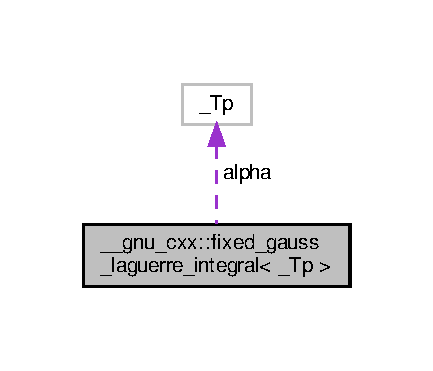
\includegraphics[width=208pt]{struct____gnu__cxx_1_1fixed__gauss__laguerre__integral__coll__graph}
\end{center}
\end{figure}
\subsection*{Public Member Functions}
\begin{DoxyCompactItemize}
\item 
\hyperlink{struct____gnu__cxx_1_1fixed__gauss__laguerre__integral_ac17e6a5bc1b597c0cda245a47ed1053a}{fixed\+\_\+gauss\+\_\+laguerre\+\_\+integral} (int n, \hyperlink{namespace____gnu__cxx_a3b19a9c800ca194374ef9172290f7d79}{\+\_\+\+Tp} \+\_\+\+\_\+alf)
\end{DoxyCompactItemize}
\subsection*{Public Attributes}
\begin{DoxyCompactItemize}
\item 
\hyperlink{namespace____gnu__cxx_a3b19a9c800ca194374ef9172290f7d79}{\+\_\+\+Tp} \hyperlink{struct____gnu__cxx_1_1fixed__gauss__laguerre__integral_a48985900ea8b5bd1104d8b977c9d9d9e}{alpha}
\item 
{\footnotesize template$<$typename \+\_\+\+Func\+Tp $>$ }\\decltype(std\+::invoke\+\_\+result\+\_\+t$<$ \+\_\+\+Func\+Tp, \hyperlink{namespace____gnu__cxx_a3b19a9c800ca194374ef9172290f7d79}{\+\_\+\+Tp} $>$\{\} $\ast$\hyperlink{namespace____gnu__cxx_a3b19a9c800ca194374ef9172290f7d79}{\+\_\+\+Tp}\{\} \hyperlink{struct____gnu__cxx_1_1fixed__gauss__laguerre__integral_aa0fcf97f3a5d830227b787378d0db399}{operator()} )(\+\_\+\+Func\+Tp \hyperlink{namespace____gnu__cxx_af2b2f0c7a2ae72b922b1afefae5a65b2}{\+\_\+\+\_\+func}, \hyperlink{namespace____gnu__cxx_a3b19a9c800ca194374ef9172290f7d79}{\+\_\+\+Tp} \+\_\+\+\_\+a, \hyperlink{namespace____gnu__cxx_a3b19a9c800ca194374ef9172290f7d79}{\+\_\+\+Tp} \+\_\+\+\_\+b) const
\item 
int \hyperlink{struct____gnu__cxx_1_1fixed__gauss__laguerre__integral_a30797226c31b897d15facc65d55c673b}{order}
\end{DoxyCompactItemize}


\subsection{Detailed Description}
\subsubsection*{template$<$typename \+\_\+\+Tp$>$\newline
struct \+\_\+\+\_\+gnu\+\_\+cxx\+::fixed\+\_\+gauss\+\_\+laguerre\+\_\+integral$<$ \+\_\+\+Tp $>$}



Definition at line 173 of file gauss\+\_\+quadrature.\+h.



\subsection{Constructor \& Destructor Documentation}
\mbox{\Hypertarget{struct____gnu__cxx_1_1fixed__gauss__laguerre__integral_ac17e6a5bc1b597c0cda245a47ed1053a}\label{struct____gnu__cxx_1_1fixed__gauss__laguerre__integral_ac17e6a5bc1b597c0cda245a47ed1053a}} 
\index{\+\_\+\+\_\+gnu\+\_\+cxx\+::fixed\+\_\+gauss\+\_\+laguerre\+\_\+integral@{\+\_\+\+\_\+gnu\+\_\+cxx\+::fixed\+\_\+gauss\+\_\+laguerre\+\_\+integral}!fixed\+\_\+gauss\+\_\+laguerre\+\_\+integral@{fixed\+\_\+gauss\+\_\+laguerre\+\_\+integral}}
\index{fixed\+\_\+gauss\+\_\+laguerre\+\_\+integral@{fixed\+\_\+gauss\+\_\+laguerre\+\_\+integral}!\+\_\+\+\_\+gnu\+\_\+cxx\+::fixed\+\_\+gauss\+\_\+laguerre\+\_\+integral@{\+\_\+\+\_\+gnu\+\_\+cxx\+::fixed\+\_\+gauss\+\_\+laguerre\+\_\+integral}}
\subsubsection{\texorpdfstring{fixed\+\_\+gauss\+\_\+laguerre\+\_\+integral()}{fixed\_gauss\_laguerre\_integral()}}
{\footnotesize\ttfamily template$<$typename \+\_\+\+Tp $>$ \\
\hyperlink{struct____gnu__cxx_1_1fixed__gauss__laguerre__integral}{\+\_\+\+\_\+gnu\+\_\+cxx\+::fixed\+\_\+gauss\+\_\+laguerre\+\_\+integral}$<$ \hyperlink{namespace____gnu__cxx_a3b19a9c800ca194374ef9172290f7d79}{\+\_\+\+Tp} $>$\+::\hyperlink{struct____gnu__cxx_1_1fixed__gauss__laguerre__integral}{fixed\+\_\+gauss\+\_\+laguerre\+\_\+integral} (\begin{DoxyParamCaption}\item[{int}]{\+\_\+\+\_\+n,  }\item[{\hyperlink{namespace____gnu__cxx_a3b19a9c800ca194374ef9172290f7d79}{\+\_\+\+Tp}}]{\+\_\+\+\_\+alf }\end{DoxyParamCaption})\hspace{0.3cm}{\ttfamily [explicit]}}

Construct a Gauss-\/\+Laguerre rule of order {\ttfamily n}.

Interval\+: $ (0, \infty) $ Weight function\+: $ x^\alpha \exp(-b(x-a)) $ Constraints\+: $ \alpha > -1 $ 

Definition at line 544 of file gauss\+\_\+quadrature.\+tcc.



References \+\_\+\+\_\+gnu\+\_\+cxx\+::\+\_\+\+\_\+func(), \+\_\+\+\_\+gnu\+\_\+cxx\+::\+\_\+\+\_\+detail\+::\+\_\+\+\_\+golub\+\_\+welsch(), \+\_\+\+\_\+gnu\+\_\+cxx\+::\+\_\+\+Ret\+Tp, \+\_\+\+\_\+gnu\+\_\+cxx\+::\+\_\+\+Tp, \+\_\+\+\_\+gnu\+\_\+cxx\+::fixed\+\_\+gauss\+\_\+laguerre\+\_\+integral$<$ \+\_\+\+Tp $>$\+::alpha, \+\_\+\+\_\+gnu\+\_\+cxx\+::fixed\+\_\+gauss\+\_\+hermite\+\_\+integral$<$ \+\_\+\+Tp $>$\+::fixed\+\_\+gauss\+\_\+hermite\+\_\+integral(), and \+\_\+\+\_\+gnu\+\_\+cxx\+::fixed\+\_\+gauss\+\_\+laguerre\+\_\+integral$<$ \+\_\+\+Tp $>$\+::order.



Referenced by \+\_\+\+\_\+gnu\+\_\+cxx\+::fixed\+\_\+gauss\+\_\+jacobi\+\_\+integral$<$ \+\_\+\+Tp $>$\+::fixed\+\_\+gauss\+\_\+jacobi\+\_\+integral().


\begin{DoxyCode}
545     : \hyperlink{struct____gnu__cxx_1_1fixed__gauss__laguerre__integral_a30797226c31b897d15facc65d55c673b}{order}(\_\_n),
546       \hyperlink{struct____gnu__cxx_1_1fixed__gauss__laguerre__integral_a48985900ea8b5bd1104d8b977c9d9d9e}{alpha}(\_\_alf),
547       point(\_\_n),
548       weight(\_\_n)
549     \{
550       \textcolor{keyword}{const} \textcolor{keyword}{auto} \_\_mu\_0 = std::tgamma(this->\hyperlink{struct____gnu__cxx_1_1fixed__gauss__laguerre__integral_a48985900ea8b5bd1104d8b977c9d9d9e}{alpha} + \hyperlink{namespace____gnu__cxx_a3b19a9c800ca194374ef9172290f7d79}{\_Tp}\{1\});
551 
552       std::vector<\_Tp> \_\_diag(this->\hyperlink{struct____gnu__cxx_1_1fixed__gauss__laguerre__integral_a30797226c31b897d15facc65d55c673b}{order});
553       std::vector<\_Tp> \_\_subd(this->\hyperlink{struct____gnu__cxx_1_1fixed__gauss__laguerre__integral_a30797226c31b897d15facc65d55c673b}{order});
554 
555       \textcolor{keywordflow}{for} (\textcolor{keywordtype}{int} \_\_i = 0; \_\_i < this->\hyperlink{struct____gnu__cxx_1_1fixed__gauss__laguerre__integral_a30797226c31b897d15facc65d55c673b}{order}; ++\_\_i)
556         \{
557           \_\_diag[\_\_i] = \hyperlink{namespace____gnu__cxx_a3b19a9c800ca194374ef9172290f7d79}{\_Tp}(2 * \_\_i + 1) + this->\hyperlink{struct____gnu__cxx_1_1fixed__gauss__laguerre__integral_a48985900ea8b5bd1104d8b977c9d9d9e}{alpha};
558           \_\_subd[\_\_i] = std::sqrt(\hyperlink{namespace____gnu__cxx_a3b19a9c800ca194374ef9172290f7d79}{\_Tp}(\_\_i + 1) * (this->\hyperlink{struct____gnu__cxx_1_1fixed__gauss__laguerre__integral_a48985900ea8b5bd1104d8b977c9d9d9e}{alpha} + \hyperlink{namespace____gnu__cxx_a3b19a9c800ca194374ef9172290f7d79}{\_Tp}(\_\_i + 1)));
559         \}
560 
561       \hyperlink{namespace____gnu__cxx_1_1____detail_aa9f299bb7c04606a9a9aab3ab9e4f4c8}{\_\_detail::\_\_golub\_welsch}(\_\_mu\_0, this->order, \_\_diag, \_\_subd,
562                                this->point, this->weight);
563     \}
\end{DoxyCode}


\subsection{Member Data Documentation}
\mbox{\Hypertarget{struct____gnu__cxx_1_1fixed__gauss__laguerre__integral_a48985900ea8b5bd1104d8b977c9d9d9e}\label{struct____gnu__cxx_1_1fixed__gauss__laguerre__integral_a48985900ea8b5bd1104d8b977c9d9d9e}} 
\index{\+\_\+\+\_\+gnu\+\_\+cxx\+::fixed\+\_\+gauss\+\_\+laguerre\+\_\+integral@{\+\_\+\+\_\+gnu\+\_\+cxx\+::fixed\+\_\+gauss\+\_\+laguerre\+\_\+integral}!alpha@{alpha}}
\index{alpha@{alpha}!\+\_\+\+\_\+gnu\+\_\+cxx\+::fixed\+\_\+gauss\+\_\+laguerre\+\_\+integral@{\+\_\+\+\_\+gnu\+\_\+cxx\+::fixed\+\_\+gauss\+\_\+laguerre\+\_\+integral}}
\subsubsection{\texorpdfstring{alpha}{alpha}}
{\footnotesize\ttfamily template$<$typename \+\_\+\+Tp$>$ \\
\hyperlink{namespace____gnu__cxx_a3b19a9c800ca194374ef9172290f7d79}{\+\_\+\+Tp} \hyperlink{struct____gnu__cxx_1_1fixed__gauss__laguerre__integral}{\+\_\+\+\_\+gnu\+\_\+cxx\+::fixed\+\_\+gauss\+\_\+laguerre\+\_\+integral}$<$ \hyperlink{namespace____gnu__cxx_a3b19a9c800ca194374ef9172290f7d79}{\+\_\+\+Tp} $>$\+::alpha}



Definition at line 176 of file gauss\+\_\+quadrature.\+h.



Referenced by \+\_\+\+\_\+gnu\+\_\+cxx\+::fixed\+\_\+gauss\+\_\+laguerre\+\_\+integral$<$ \+\_\+\+Tp $>$\+::fixed\+\_\+gauss\+\_\+laguerre\+\_\+integral().

\mbox{\Hypertarget{struct____gnu__cxx_1_1fixed__gauss__laguerre__integral_aa0fcf97f3a5d830227b787378d0db399}\label{struct____gnu__cxx_1_1fixed__gauss__laguerre__integral_aa0fcf97f3a5d830227b787378d0db399}} 
\index{\+\_\+\+\_\+gnu\+\_\+cxx\+::fixed\+\_\+gauss\+\_\+laguerre\+\_\+integral@{\+\_\+\+\_\+gnu\+\_\+cxx\+::fixed\+\_\+gauss\+\_\+laguerre\+\_\+integral}!operator()@{operator()}}
\index{operator()@{operator()}!\+\_\+\+\_\+gnu\+\_\+cxx\+::fixed\+\_\+gauss\+\_\+laguerre\+\_\+integral@{\+\_\+\+\_\+gnu\+\_\+cxx\+::fixed\+\_\+gauss\+\_\+laguerre\+\_\+integral}}
\subsubsection{\texorpdfstring{operator()}{operator()}}
{\footnotesize\ttfamily template$<$typename \+\_\+\+Tp$>$ \\
template$<$typename \+\_\+\+Func\+Tp $>$ \\
decltype(std\+::invoke\+\_\+result\+\_\+t$<$\+\_\+\+Func\+Tp, \hyperlink{namespace____gnu__cxx_a3b19a9c800ca194374ef9172290f7d79}{\+\_\+\+Tp}$>$\{\} $\ast$ \hyperlink{namespace____gnu__cxx_a3b19a9c800ca194374ef9172290f7d79}{\+\_\+\+Tp}\{\} \hyperlink{struct____gnu__cxx_1_1fixed__gauss__laguerre__integral}{\+\_\+\+\_\+gnu\+\_\+cxx\+::fixed\+\_\+gauss\+\_\+laguerre\+\_\+integral}$<$ \hyperlink{namespace____gnu__cxx_a3b19a9c800ca194374ef9172290f7d79}{\+\_\+\+Tp} $>$\+::operator()) (\+\_\+\+Func\+Tp \hyperlink{namespace____gnu__cxx_af2b2f0c7a2ae72b922b1afefae5a65b2}{\+\_\+\+\_\+func}, \hyperlink{namespace____gnu__cxx_a3b19a9c800ca194374ef9172290f7d79}{\+\_\+\+Tp} \+\_\+\+\_\+a, \hyperlink{namespace____gnu__cxx_a3b19a9c800ca194374ef9172290f7d79}{\+\_\+\+Tp} \+\_\+\+\_\+b) const}



Definition at line 182 of file gauss\+\_\+quadrature.\+h.

\mbox{\Hypertarget{struct____gnu__cxx_1_1fixed__gauss__laguerre__integral_a30797226c31b897d15facc65d55c673b}\label{struct____gnu__cxx_1_1fixed__gauss__laguerre__integral_a30797226c31b897d15facc65d55c673b}} 
\index{\+\_\+\+\_\+gnu\+\_\+cxx\+::fixed\+\_\+gauss\+\_\+laguerre\+\_\+integral@{\+\_\+\+\_\+gnu\+\_\+cxx\+::fixed\+\_\+gauss\+\_\+laguerre\+\_\+integral}!order@{order}}
\index{order@{order}!\+\_\+\+\_\+gnu\+\_\+cxx\+::fixed\+\_\+gauss\+\_\+laguerre\+\_\+integral@{\+\_\+\+\_\+gnu\+\_\+cxx\+::fixed\+\_\+gauss\+\_\+laguerre\+\_\+integral}}
\subsubsection{\texorpdfstring{order}{order}}
{\footnotesize\ttfamily template$<$typename \+\_\+\+Tp$>$ \\
int \hyperlink{struct____gnu__cxx_1_1fixed__gauss__laguerre__integral}{\+\_\+\+\_\+gnu\+\_\+cxx\+::fixed\+\_\+gauss\+\_\+laguerre\+\_\+integral}$<$ \hyperlink{namespace____gnu__cxx_a3b19a9c800ca194374ef9172290f7d79}{\+\_\+\+Tp} $>$\+::order}



Definition at line 175 of file gauss\+\_\+quadrature.\+h.



Referenced by \+\_\+\+\_\+gnu\+\_\+cxx\+::fixed\+\_\+gauss\+\_\+laguerre\+\_\+integral$<$ \+\_\+\+Tp $>$\+::fixed\+\_\+gauss\+\_\+laguerre\+\_\+integral().



The documentation for this struct was generated from the following files\+:\begin{DoxyCompactItemize}
\item 
include/ext/\hyperlink{gauss__quadrature_8h}{gauss\+\_\+quadrature.\+h}\item 
include/ext/\hyperlink{gauss__quadrature_8tcc}{gauss\+\_\+quadrature.\+tcc}\end{DoxyCompactItemize}

\hypertarget{struct____gnu__cxx_1_1fixed__gauss__legendre__integral}{}\section{\+\_\+\+\_\+gnu\+\_\+cxx\+:\+:fixed\+\_\+gauss\+\_\+legendre\+\_\+integral$<$ \+\_\+\+Tp $>$ Struct Template Reference}
\label{struct____gnu__cxx_1_1fixed__gauss__legendre__integral}\index{\+\_\+\+\_\+gnu\+\_\+cxx\+::fixed\+\_\+gauss\+\_\+legendre\+\_\+integral$<$ \+\_\+\+Tp $>$@{\+\_\+\+\_\+gnu\+\_\+cxx\+::fixed\+\_\+gauss\+\_\+legendre\+\_\+integral$<$ \+\_\+\+Tp $>$}}


{\ttfamily \#include $<$gauss\+\_\+quadrature.\+h$>$}

\subsection*{Public Member Functions}
\begin{DoxyCompactItemize}
\item 
\hyperlink{struct____gnu__cxx_1_1fixed__gauss__legendre__integral_ad5210c037dcd806afb26e1888ce9676f}{fixed\+\_\+gauss\+\_\+legendre\+\_\+integral} (int \+\_\+\+\_\+n)
\end{DoxyCompactItemize}
\subsection*{Public Attributes}
\begin{DoxyCompactItemize}
\item 
{\footnotesize template$<$typename \+\_\+\+Func\+Tp $>$ }\\decltype(std\+::invoke\+\_\+result\+\_\+t$<$ \+\_\+\+Func\+Tp, \hyperlink{namespace____gnu__cxx_a3b19a9c800ca194374ef9172290f7d79}{\+\_\+\+Tp} $>$\{\} $\ast$\hyperlink{namespace____gnu__cxx_a3b19a9c800ca194374ef9172290f7d79}{\+\_\+\+Tp}\{\} \hyperlink{struct____gnu__cxx_1_1fixed__gauss__legendre__integral_aa6a0f40e1c8dba2864c88401fea3067d}{operator()} )(\+\_\+\+Func\+Tp \hyperlink{namespace____gnu__cxx_af2b2f0c7a2ae72b922b1afefae5a65b2}{\+\_\+\+\_\+func}, \hyperlink{namespace____gnu__cxx_a3b19a9c800ca194374ef9172290f7d79}{\+\_\+\+Tp} \+\_\+\+\_\+a, \hyperlink{namespace____gnu__cxx_a3b19a9c800ca194374ef9172290f7d79}{\+\_\+\+Tp} \+\_\+\+\_\+b) const
\item 
int \hyperlink{struct____gnu__cxx_1_1fixed__gauss__legendre__integral_a51724253e7545ed73de4be77aabf951a}{order}
\end{DoxyCompactItemize}


\subsection{Detailed Description}
\subsubsection*{template$<$typename \+\_\+\+Tp$>$\newline
struct \+\_\+\+\_\+gnu\+\_\+cxx\+::fixed\+\_\+gauss\+\_\+legendre\+\_\+integral$<$ \+\_\+\+Tp $>$}

Build the absiscae and weights of a Gauss quadrature rule from a symmetric tridiagonal Jacobi matrix. 

Definition at line 34 of file gauss\+\_\+quadrature.\+h.



\subsection{Constructor \& Destructor Documentation}
\mbox{\Hypertarget{struct____gnu__cxx_1_1fixed__gauss__legendre__integral_ad5210c037dcd806afb26e1888ce9676f}\label{struct____gnu__cxx_1_1fixed__gauss__legendre__integral_ad5210c037dcd806afb26e1888ce9676f}} 
\index{\+\_\+\+\_\+gnu\+\_\+cxx\+::fixed\+\_\+gauss\+\_\+legendre\+\_\+integral@{\+\_\+\+\_\+gnu\+\_\+cxx\+::fixed\+\_\+gauss\+\_\+legendre\+\_\+integral}!fixed\+\_\+gauss\+\_\+legendre\+\_\+integral@{fixed\+\_\+gauss\+\_\+legendre\+\_\+integral}}
\index{fixed\+\_\+gauss\+\_\+legendre\+\_\+integral@{fixed\+\_\+gauss\+\_\+legendre\+\_\+integral}!\+\_\+\+\_\+gnu\+\_\+cxx\+::fixed\+\_\+gauss\+\_\+legendre\+\_\+integral@{\+\_\+\+\_\+gnu\+\_\+cxx\+::fixed\+\_\+gauss\+\_\+legendre\+\_\+integral}}
\subsubsection{\texorpdfstring{fixed\+\_\+gauss\+\_\+legendre\+\_\+integral()}{fixed\_gauss\_legendre\_integral()}}
{\footnotesize\ttfamily template$<$typename \+\_\+\+Tp $>$ \\
\hyperlink{struct____gnu__cxx_1_1fixed__gauss__legendre__integral}{\+\_\+\+\_\+gnu\+\_\+cxx\+::fixed\+\_\+gauss\+\_\+legendre\+\_\+integral}$<$ \hyperlink{namespace____gnu__cxx_a3b19a9c800ca194374ef9172290f7d79}{\+\_\+\+Tp} $>$\+::\hyperlink{struct____gnu__cxx_1_1fixed__gauss__legendre__integral}{fixed\+\_\+gauss\+\_\+legendre\+\_\+integral} (\begin{DoxyParamCaption}\item[{int}]{\+\_\+\+\_\+n }\end{DoxyParamCaption})\hspace{0.3cm}{\ttfamily [explicit]}}

Construct a Gauss-\/\+Legendre rule of order {\ttfamily n}.

Weight function\+: $ 1 $ Constraints\+: $ b > a $ 

Definition at line 88 of file gauss\+\_\+quadrature.\+tcc.



References \+\_\+\+\_\+gnu\+\_\+cxx\+::\+\_\+\+\_\+func(), \+\_\+\+\_\+gnu\+\_\+cxx\+::\+\_\+\+\_\+detail\+::\+\_\+\+\_\+golub\+\_\+welsch(), \+\_\+\+\_\+gnu\+\_\+cxx\+::\+\_\+\+Ret\+Tp, \+\_\+\+\_\+gnu\+\_\+cxx\+::\+\_\+\+Tp, \+\_\+\+\_\+gnu\+\_\+cxx\+::fixed\+\_\+gauss\+\_\+chebyshev\+\_\+t\+\_\+integral$<$ \+\_\+\+Tp $>$\+::fixed\+\_\+gauss\+\_\+chebyshev\+\_\+t\+\_\+integral(), and \+\_\+\+\_\+gnu\+\_\+cxx\+::fixed\+\_\+gauss\+\_\+legendre\+\_\+integral$<$ \+\_\+\+Tp $>$\+::order.



Referenced by \+\_\+\+\_\+gnu\+\_\+cxx\+::\+\_\+\+\_\+detail\+::\+\_\+\+\_\+golub\+\_\+welsch().


\begin{DoxyCode}
89     : \hyperlink{struct____gnu__cxx_1_1fixed__gauss__legendre__integral_a51724253e7545ed73de4be77aabf951a}{order}(\_\_n),
90       point(\_\_n),
91       weight(\_\_n)
92     \{
93       \textcolor{keyword}{const} \textcolor{keyword}{auto} \_\_mu\_0 = \hyperlink{namespace____gnu__cxx_a3b19a9c800ca194374ef9172290f7d79}{\_Tp}\{2\};
94 
95       std::vector<\_Tp> \_\_diag(this->\hyperlink{struct____gnu__cxx_1_1fixed__gauss__legendre__integral_a51724253e7545ed73de4be77aabf951a}{order}, \hyperlink{namespace____gnu__cxx_a3b19a9c800ca194374ef9172290f7d79}{\_Tp}\{0\});
96       std::vector<\_Tp> \_\_subd(this->\hyperlink{struct____gnu__cxx_1_1fixed__gauss__legendre__integral_a51724253e7545ed73de4be77aabf951a}{order});
97 
98       \textcolor{keywordflow}{for} (\textcolor{keywordtype}{int} \_\_i = 1; \_\_i <= this->\hyperlink{struct____gnu__cxx_1_1fixed__gauss__legendre__integral_a51724253e7545ed73de4be77aabf951a}{order}; ++\_\_i)
99         \_\_subd[\_\_i - 1] = \hyperlink{namespace____gnu__cxx_a3b19a9c800ca194374ef9172290f7d79}{\_Tp}(\_\_i) / std::sqrt(\hyperlink{namespace____gnu__cxx_a3b19a9c800ca194374ef9172290f7d79}{\_Tp}(4 * \_\_i * \_\_i - 1));
100 
101       \hyperlink{namespace____gnu__cxx_1_1____detail_aa9f299bb7c04606a9a9aab3ab9e4f4c8}{\_\_detail::\_\_golub\_welsch}(\_\_mu\_0, this->\hyperlink{struct____gnu__cxx_1_1fixed__gauss__legendre__integral_a51724253e7545ed73de4be77aabf951a}{order}, \_\_diag, \_\_subd,
102                                this->point, this->weight);
103     \}
\end{DoxyCode}


\subsection{Member Data Documentation}
\mbox{\Hypertarget{struct____gnu__cxx_1_1fixed__gauss__legendre__integral_aa6a0f40e1c8dba2864c88401fea3067d}\label{struct____gnu__cxx_1_1fixed__gauss__legendre__integral_aa6a0f40e1c8dba2864c88401fea3067d}} 
\index{\+\_\+\+\_\+gnu\+\_\+cxx\+::fixed\+\_\+gauss\+\_\+legendre\+\_\+integral@{\+\_\+\+\_\+gnu\+\_\+cxx\+::fixed\+\_\+gauss\+\_\+legendre\+\_\+integral}!operator()@{operator()}}
\index{operator()@{operator()}!\+\_\+\+\_\+gnu\+\_\+cxx\+::fixed\+\_\+gauss\+\_\+legendre\+\_\+integral@{\+\_\+\+\_\+gnu\+\_\+cxx\+::fixed\+\_\+gauss\+\_\+legendre\+\_\+integral}}
\subsubsection{\texorpdfstring{operator()}{operator()}}
{\footnotesize\ttfamily template$<$typename \+\_\+\+Tp$>$ \\
template$<$typename \+\_\+\+Func\+Tp $>$ \\
decltype(std\+::invoke\+\_\+result\+\_\+t$<$\+\_\+\+Func\+Tp, \hyperlink{namespace____gnu__cxx_a3b19a9c800ca194374ef9172290f7d79}{\+\_\+\+Tp}$>$\{\} $\ast$ \hyperlink{namespace____gnu__cxx_a3b19a9c800ca194374ef9172290f7d79}{\+\_\+\+Tp}\{\} \hyperlink{struct____gnu__cxx_1_1fixed__gauss__legendre__integral}{\+\_\+\+\_\+gnu\+\_\+cxx\+::fixed\+\_\+gauss\+\_\+legendre\+\_\+integral}$<$ \hyperlink{namespace____gnu__cxx_a3b19a9c800ca194374ef9172290f7d79}{\+\_\+\+Tp} $>$\+::operator()) (\+\_\+\+Func\+Tp \hyperlink{namespace____gnu__cxx_af2b2f0c7a2ae72b922b1afefae5a65b2}{\+\_\+\+\_\+func}, \hyperlink{namespace____gnu__cxx_a3b19a9c800ca194374ef9172290f7d79}{\+\_\+\+Tp} \+\_\+\+\_\+a, \hyperlink{namespace____gnu__cxx_a3b19a9c800ca194374ef9172290f7d79}{\+\_\+\+Tp} \+\_\+\+\_\+b) const}



Definition at line 42 of file gauss\+\_\+quadrature.\+h.

\mbox{\Hypertarget{struct____gnu__cxx_1_1fixed__gauss__legendre__integral_a51724253e7545ed73de4be77aabf951a}\label{struct____gnu__cxx_1_1fixed__gauss__legendre__integral_a51724253e7545ed73de4be77aabf951a}} 
\index{\+\_\+\+\_\+gnu\+\_\+cxx\+::fixed\+\_\+gauss\+\_\+legendre\+\_\+integral@{\+\_\+\+\_\+gnu\+\_\+cxx\+::fixed\+\_\+gauss\+\_\+legendre\+\_\+integral}!order@{order}}
\index{order@{order}!\+\_\+\+\_\+gnu\+\_\+cxx\+::fixed\+\_\+gauss\+\_\+legendre\+\_\+integral@{\+\_\+\+\_\+gnu\+\_\+cxx\+::fixed\+\_\+gauss\+\_\+legendre\+\_\+integral}}
\subsubsection{\texorpdfstring{order}{order}}
{\footnotesize\ttfamily template$<$typename \+\_\+\+Tp$>$ \\
int \hyperlink{struct____gnu__cxx_1_1fixed__gauss__legendre__integral}{\+\_\+\+\_\+gnu\+\_\+cxx\+::fixed\+\_\+gauss\+\_\+legendre\+\_\+integral}$<$ \hyperlink{namespace____gnu__cxx_a3b19a9c800ca194374ef9172290f7d79}{\+\_\+\+Tp} $>$\+::order}



Definition at line 36 of file gauss\+\_\+quadrature.\+h.



Referenced by \+\_\+\+\_\+gnu\+\_\+cxx\+::fixed\+\_\+gauss\+\_\+legendre\+\_\+integral$<$ \+\_\+\+Tp $>$\+::fixed\+\_\+gauss\+\_\+legendre\+\_\+integral().



The documentation for this struct was generated from the following files\+:\begin{DoxyCompactItemize}
\item 
include/ext/\hyperlink{gauss__quadrature_8h}{gauss\+\_\+quadrature.\+h}\item 
include/ext/\hyperlink{gauss__quadrature_8tcc}{gauss\+\_\+quadrature.\+tcc}\end{DoxyCompactItemize}

\hypertarget{struct____gnu__cxx_1_1fixed__gauss__rational__integral}{}\section{\+\_\+\+\_\+gnu\+\_\+cxx\+:\+:fixed\+\_\+gauss\+\_\+rational\+\_\+integral$<$ \+\_\+\+Tp $>$ Struct Template Reference}
\label{struct____gnu__cxx_1_1fixed__gauss__rational__integral}\index{\+\_\+\+\_\+gnu\+\_\+cxx\+::fixed\+\_\+gauss\+\_\+rational\+\_\+integral$<$ \+\_\+\+Tp $>$@{\+\_\+\+\_\+gnu\+\_\+cxx\+::fixed\+\_\+gauss\+\_\+rational\+\_\+integral$<$ \+\_\+\+Tp $>$}}


{\ttfamily \#include $<$gauss\+\_\+quadrature.\+h$>$}



Collaboration diagram for \+\_\+\+\_\+gnu\+\_\+cxx\+:\+:fixed\+\_\+gauss\+\_\+rational\+\_\+integral$<$ \+\_\+\+Tp $>$\+:
\nopagebreak
\begin{figure}[H]
\begin{center}
\leavevmode
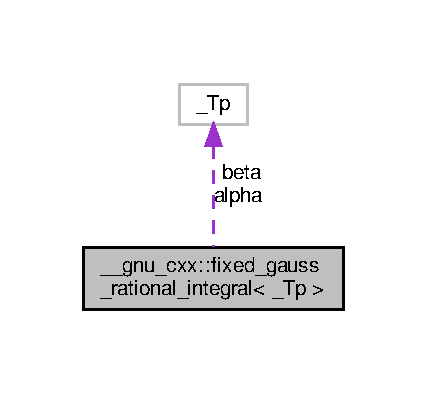
\includegraphics[width=205pt]{struct____gnu__cxx_1_1fixed__gauss__rational__integral__coll__graph}
\end{center}
\end{figure}
\subsection*{Public Member Functions}
\begin{DoxyCompactItemize}
\item 
\hyperlink{struct____gnu__cxx_1_1fixed__gauss__rational__integral_a794a8d9a4f972549c1416f2275ea3180}{fixed\+\_\+gauss\+\_\+rational\+\_\+integral} (int \+\_\+\+\_\+n, \hyperlink{namespace____gnu__cxx_a3b19a9c800ca194374ef9172290f7d79}{\+\_\+\+Tp} \+\_\+\+\_\+alf, \hyperlink{namespace____gnu__cxx_a3b19a9c800ca194374ef9172290f7d79}{\+\_\+\+Tp} \+\_\+\+\_\+bet)
\end{DoxyCompactItemize}
\subsection*{Public Attributes}
\begin{DoxyCompactItemize}
\item 
\hyperlink{namespace____gnu__cxx_a3b19a9c800ca194374ef9172290f7d79}{\+\_\+\+Tp} \hyperlink{struct____gnu__cxx_1_1fixed__gauss__rational__integral_afce7345b6772928485c8d6ce8e08769b}{alpha}
\item 
\hyperlink{namespace____gnu__cxx_a3b19a9c800ca194374ef9172290f7d79}{\+\_\+\+Tp} \hyperlink{struct____gnu__cxx_1_1fixed__gauss__rational__integral_aa6c563ee188859be79a987b67312d7ac}{beta}
\item 
{\footnotesize template$<$typename \+\_\+\+Func\+Tp $>$ }\\decltype(std\+::invoke\+\_\+result\+\_\+t$<$ \+\_\+\+Func\+Tp, \hyperlink{namespace____gnu__cxx_a3b19a9c800ca194374ef9172290f7d79}{\+\_\+\+Tp} $>$\{\} $\ast$\hyperlink{namespace____gnu__cxx_a3b19a9c800ca194374ef9172290f7d79}{\+\_\+\+Tp}\{\} \hyperlink{struct____gnu__cxx_1_1fixed__gauss__rational__integral_aa58df016c4139a1001cd3b155cc50256}{operator()} )(\+\_\+\+Func\+Tp \hyperlink{namespace____gnu__cxx_af2b2f0c7a2ae72b922b1afefae5a65b2}{\+\_\+\+\_\+func}, \hyperlink{namespace____gnu__cxx_a3b19a9c800ca194374ef9172290f7d79}{\+\_\+\+Tp} \+\_\+\+\_\+a, \hyperlink{namespace____gnu__cxx_a3b19a9c800ca194374ef9172290f7d79}{\+\_\+\+Tp} \+\_\+\+\_\+b) const
\item 
int \hyperlink{struct____gnu__cxx_1_1fixed__gauss__rational__integral_a5998f7b5975013c67c95c2bacc279857}{order}
\end{DoxyCompactItemize}


\subsection{Detailed Description}
\subsubsection*{template$<$typename \+\_\+\+Tp$>$\newline
struct \+\_\+\+\_\+gnu\+\_\+cxx\+::fixed\+\_\+gauss\+\_\+rational\+\_\+integral$<$ \+\_\+\+Tp $>$}



Definition at line 233 of file gauss\+\_\+quadrature.\+h.



\subsection{Constructor \& Destructor Documentation}
\mbox{\Hypertarget{struct____gnu__cxx_1_1fixed__gauss__rational__integral_a794a8d9a4f972549c1416f2275ea3180}\label{struct____gnu__cxx_1_1fixed__gauss__rational__integral_a794a8d9a4f972549c1416f2275ea3180}} 
\index{\+\_\+\+\_\+gnu\+\_\+cxx\+::fixed\+\_\+gauss\+\_\+rational\+\_\+integral@{\+\_\+\+\_\+gnu\+\_\+cxx\+::fixed\+\_\+gauss\+\_\+rational\+\_\+integral}!fixed\+\_\+gauss\+\_\+rational\+\_\+integral@{fixed\+\_\+gauss\+\_\+rational\+\_\+integral}}
\index{fixed\+\_\+gauss\+\_\+rational\+\_\+integral@{fixed\+\_\+gauss\+\_\+rational\+\_\+integral}!\+\_\+\+\_\+gnu\+\_\+cxx\+::fixed\+\_\+gauss\+\_\+rational\+\_\+integral@{\+\_\+\+\_\+gnu\+\_\+cxx\+::fixed\+\_\+gauss\+\_\+rational\+\_\+integral}}
\subsubsection{\texorpdfstring{fixed\+\_\+gauss\+\_\+rational\+\_\+integral()}{fixed\_gauss\_rational\_integral()}}
{\footnotesize\ttfamily template$<$typename \+\_\+\+Tp$>$ \\
\hyperlink{struct____gnu__cxx_1_1fixed__gauss__rational__integral}{\+\_\+\+\_\+gnu\+\_\+cxx\+::fixed\+\_\+gauss\+\_\+rational\+\_\+integral}$<$ \hyperlink{namespace____gnu__cxx_a3b19a9c800ca194374ef9172290f7d79}{\+\_\+\+Tp} $>$\+::\hyperlink{struct____gnu__cxx_1_1fixed__gauss__rational__integral}{fixed\+\_\+gauss\+\_\+rational\+\_\+integral} (\begin{DoxyParamCaption}\item[{int}]{\+\_\+\+\_\+n,  }\item[{\hyperlink{namespace____gnu__cxx_a3b19a9c800ca194374ef9172290f7d79}{\+\_\+\+Tp}}]{\+\_\+\+\_\+alf,  }\item[{\hyperlink{namespace____gnu__cxx_a3b19a9c800ca194374ef9172290f7d79}{\+\_\+\+Tp}}]{\+\_\+\+\_\+bet }\end{DoxyParamCaption})\hspace{0.3cm}{\ttfamily [explicit]}}



Referenced by \+\_\+\+\_\+gnu\+\_\+cxx\+::fixed\+\_\+gauss\+\_\+exponential\+\_\+integral$<$ \+\_\+\+Tp $>$\+::fixed\+\_\+gauss\+\_\+exponential\+\_\+integral().



\subsection{Member Data Documentation}
\mbox{\Hypertarget{struct____gnu__cxx_1_1fixed__gauss__rational__integral_afce7345b6772928485c8d6ce8e08769b}\label{struct____gnu__cxx_1_1fixed__gauss__rational__integral_afce7345b6772928485c8d6ce8e08769b}} 
\index{\+\_\+\+\_\+gnu\+\_\+cxx\+::fixed\+\_\+gauss\+\_\+rational\+\_\+integral@{\+\_\+\+\_\+gnu\+\_\+cxx\+::fixed\+\_\+gauss\+\_\+rational\+\_\+integral}!alpha@{alpha}}
\index{alpha@{alpha}!\+\_\+\+\_\+gnu\+\_\+cxx\+::fixed\+\_\+gauss\+\_\+rational\+\_\+integral@{\+\_\+\+\_\+gnu\+\_\+cxx\+::fixed\+\_\+gauss\+\_\+rational\+\_\+integral}}
\subsubsection{\texorpdfstring{alpha}{alpha}}
{\footnotesize\ttfamily template$<$typename \+\_\+\+Tp$>$ \\
\hyperlink{namespace____gnu__cxx_a3b19a9c800ca194374ef9172290f7d79}{\+\_\+\+Tp} \hyperlink{struct____gnu__cxx_1_1fixed__gauss__rational__integral}{\+\_\+\+\_\+gnu\+\_\+cxx\+::fixed\+\_\+gauss\+\_\+rational\+\_\+integral}$<$ \hyperlink{namespace____gnu__cxx_a3b19a9c800ca194374ef9172290f7d79}{\+\_\+\+Tp} $>$\+::alpha}



Definition at line 236 of file gauss\+\_\+quadrature.\+h.

\mbox{\Hypertarget{struct____gnu__cxx_1_1fixed__gauss__rational__integral_aa6c563ee188859be79a987b67312d7ac}\label{struct____gnu__cxx_1_1fixed__gauss__rational__integral_aa6c563ee188859be79a987b67312d7ac}} 
\index{\+\_\+\+\_\+gnu\+\_\+cxx\+::fixed\+\_\+gauss\+\_\+rational\+\_\+integral@{\+\_\+\+\_\+gnu\+\_\+cxx\+::fixed\+\_\+gauss\+\_\+rational\+\_\+integral}!beta@{beta}}
\index{beta@{beta}!\+\_\+\+\_\+gnu\+\_\+cxx\+::fixed\+\_\+gauss\+\_\+rational\+\_\+integral@{\+\_\+\+\_\+gnu\+\_\+cxx\+::fixed\+\_\+gauss\+\_\+rational\+\_\+integral}}
\subsubsection{\texorpdfstring{beta}{beta}}
{\footnotesize\ttfamily template$<$typename \+\_\+\+Tp$>$ \\
\hyperlink{namespace____gnu__cxx_a3b19a9c800ca194374ef9172290f7d79}{\+\_\+\+Tp} \hyperlink{struct____gnu__cxx_1_1fixed__gauss__rational__integral}{\+\_\+\+\_\+gnu\+\_\+cxx\+::fixed\+\_\+gauss\+\_\+rational\+\_\+integral}$<$ \hyperlink{namespace____gnu__cxx_a3b19a9c800ca194374ef9172290f7d79}{\+\_\+\+Tp} $>$\+::beta}



Definition at line 237 of file gauss\+\_\+quadrature.\+h.

\mbox{\Hypertarget{struct____gnu__cxx_1_1fixed__gauss__rational__integral_aa58df016c4139a1001cd3b155cc50256}\label{struct____gnu__cxx_1_1fixed__gauss__rational__integral_aa58df016c4139a1001cd3b155cc50256}} 
\index{\+\_\+\+\_\+gnu\+\_\+cxx\+::fixed\+\_\+gauss\+\_\+rational\+\_\+integral@{\+\_\+\+\_\+gnu\+\_\+cxx\+::fixed\+\_\+gauss\+\_\+rational\+\_\+integral}!operator()@{operator()}}
\index{operator()@{operator()}!\+\_\+\+\_\+gnu\+\_\+cxx\+::fixed\+\_\+gauss\+\_\+rational\+\_\+integral@{\+\_\+\+\_\+gnu\+\_\+cxx\+::fixed\+\_\+gauss\+\_\+rational\+\_\+integral}}
\subsubsection{\texorpdfstring{operator()}{operator()}}
{\footnotesize\ttfamily template$<$typename \+\_\+\+Tp$>$ \\
template$<$typename \+\_\+\+Func\+Tp $>$ \\
decltype(std\+::invoke\+\_\+result\+\_\+t$<$\+\_\+\+Func\+Tp, \hyperlink{namespace____gnu__cxx_a3b19a9c800ca194374ef9172290f7d79}{\+\_\+\+Tp}$>$\{\} $\ast$ \hyperlink{namespace____gnu__cxx_a3b19a9c800ca194374ef9172290f7d79}{\+\_\+\+Tp}\{\} \hyperlink{struct____gnu__cxx_1_1fixed__gauss__rational__integral}{\+\_\+\+\_\+gnu\+\_\+cxx\+::fixed\+\_\+gauss\+\_\+rational\+\_\+integral}$<$ \hyperlink{namespace____gnu__cxx_a3b19a9c800ca194374ef9172290f7d79}{\+\_\+\+Tp} $>$\+::operator()) (\+\_\+\+Func\+Tp \hyperlink{namespace____gnu__cxx_af2b2f0c7a2ae72b922b1afefae5a65b2}{\+\_\+\+\_\+func}, \hyperlink{namespace____gnu__cxx_a3b19a9c800ca194374ef9172290f7d79}{\+\_\+\+Tp} \+\_\+\+\_\+a, \hyperlink{namespace____gnu__cxx_a3b19a9c800ca194374ef9172290f7d79}{\+\_\+\+Tp} \+\_\+\+\_\+b) const}



Definition at line 243 of file gauss\+\_\+quadrature.\+h.

\mbox{\Hypertarget{struct____gnu__cxx_1_1fixed__gauss__rational__integral_a5998f7b5975013c67c95c2bacc279857}\label{struct____gnu__cxx_1_1fixed__gauss__rational__integral_a5998f7b5975013c67c95c2bacc279857}} 
\index{\+\_\+\+\_\+gnu\+\_\+cxx\+::fixed\+\_\+gauss\+\_\+rational\+\_\+integral@{\+\_\+\+\_\+gnu\+\_\+cxx\+::fixed\+\_\+gauss\+\_\+rational\+\_\+integral}!order@{order}}
\index{order@{order}!\+\_\+\+\_\+gnu\+\_\+cxx\+::fixed\+\_\+gauss\+\_\+rational\+\_\+integral@{\+\_\+\+\_\+gnu\+\_\+cxx\+::fixed\+\_\+gauss\+\_\+rational\+\_\+integral}}
\subsubsection{\texorpdfstring{order}{order}}
{\footnotesize\ttfamily template$<$typename \+\_\+\+Tp$>$ \\
int \hyperlink{struct____gnu__cxx_1_1fixed__gauss__rational__integral}{\+\_\+\+\_\+gnu\+\_\+cxx\+::fixed\+\_\+gauss\+\_\+rational\+\_\+integral}$<$ \hyperlink{namespace____gnu__cxx_a3b19a9c800ca194374ef9172290f7d79}{\+\_\+\+Tp} $>$\+::order}



Definition at line 235 of file gauss\+\_\+quadrature.\+h.



The documentation for this struct was generated from the following file\+:\begin{DoxyCompactItemize}
\item 
include/ext/\hyperlink{gauss__quadrature_8h}{gauss\+\_\+quadrature.\+h}\end{DoxyCompactItemize}

\hypertarget{struct____gnu__cxx_1_1fixed__integral__t}{}\section{\+\_\+\+\_\+gnu\+\_\+cxx\+:\+:fixed\+\_\+integral\+\_\+t$<$ \+\_\+\+Tp, \+\_\+\+Ret\+Tp $>$ Struct Template Reference}
\label{struct____gnu__cxx_1_1fixed__integral__t}\index{\+\_\+\+\_\+gnu\+\_\+cxx\+::fixed\+\_\+integral\+\_\+t$<$ \+\_\+\+Tp, \+\_\+\+Ret\+Tp $>$@{\+\_\+\+\_\+gnu\+\_\+cxx\+::fixed\+\_\+integral\+\_\+t$<$ \+\_\+\+Tp, \+\_\+\+Ret\+Tp $>$}}


{\ttfamily \#include $<$integration.\+h$>$}

\subsection*{Public Types}
\begin{DoxyCompactItemize}
\item 
using \hyperlink{struct____gnu__cxx_1_1fixed__integral__t_a68a11ba646968b5cebfc4cc7c1547478}{\+\_\+\+Area\+Tp} = decltype(\hyperlink{namespace____gnu__cxx_a886e03ece3d53ff7fa6c098a40f93fa5}{\+\_\+\+Ret\+Tp}\{\} $\ast$\hyperlink{namespace____gnu__cxx_a3b19a9c800ca194374ef9172290f7d79}{\+\_\+\+Tp}\{\})
\end{DoxyCompactItemize}
\subsection*{Public Attributes}
\begin{DoxyCompactItemize}
\item 
\hyperlink{struct____gnu__cxx_1_1fixed__integral__t_a68a11ba646968b5cebfc4cc7c1547478}{\+\_\+\+Area\+Tp} \hyperlink{struct____gnu__cxx_1_1fixed__integral__t_a9d52eafc8db2db186dee1587be02d7bd}{\+\_\+\+\_\+result} = \hyperlink{struct____gnu__cxx_1_1fixed__integral__t_a68a11ba646968b5cebfc4cc7c1547478}{\+\_\+\+Area\+Tp}\{\}
\begin{DoxyCompactList}\small\item\em Result of the integral. \end{DoxyCompactList}\end{DoxyCompactItemize}


\subsection{Detailed Description}
\subsubsection*{template$<$typename \+\_\+\+Tp, typename \+\_\+\+Ret\+Tp$>$\newline
struct \+\_\+\+\_\+gnu\+\_\+cxx\+::fixed\+\_\+integral\+\_\+t$<$ \+\_\+\+Tp, \+\_\+\+Ret\+Tp $>$}

The return type for a fixed integral rule. Fixed integral types could return errors too! Globally vs. locally adaptive integrals need to be distinguished. abs(diff) vs. diff(abs) is also a thing. 

Definition at line 43 of file integration.\+h.



\subsection{Member Typedef Documentation}
\mbox{\Hypertarget{struct____gnu__cxx_1_1fixed__integral__t_a68a11ba646968b5cebfc4cc7c1547478}\label{struct____gnu__cxx_1_1fixed__integral__t_a68a11ba646968b5cebfc4cc7c1547478}} 
\index{\+\_\+\+\_\+gnu\+\_\+cxx\+::fixed\+\_\+integral\+\_\+t@{\+\_\+\+\_\+gnu\+\_\+cxx\+::fixed\+\_\+integral\+\_\+t}!\+\_\+\+Area\+Tp@{\+\_\+\+Area\+Tp}}
\index{\+\_\+\+Area\+Tp@{\+\_\+\+Area\+Tp}!\+\_\+\+\_\+gnu\+\_\+cxx\+::fixed\+\_\+integral\+\_\+t@{\+\_\+\+\_\+gnu\+\_\+cxx\+::fixed\+\_\+integral\+\_\+t}}
\subsubsection{\texorpdfstring{\+\_\+\+Area\+Tp}{\_AreaTp}}
{\footnotesize\ttfamily template$<$typename \+\_\+\+Tp, typename \+\_\+\+Ret\+Tp$>$ \\
using \hyperlink{struct____gnu__cxx_1_1fixed__integral__t}{\+\_\+\+\_\+gnu\+\_\+cxx\+::fixed\+\_\+integral\+\_\+t}$<$ \hyperlink{namespace____gnu__cxx_a3b19a9c800ca194374ef9172290f7d79}{\+\_\+\+Tp}, \hyperlink{namespace____gnu__cxx_a886e03ece3d53ff7fa6c098a40f93fa5}{\+\_\+\+Ret\+Tp} $>$\+::\hyperlink{struct____gnu__cxx_1_1fixed__integral__t_a68a11ba646968b5cebfc4cc7c1547478}{\+\_\+\+Area\+Tp} =  decltype(\hyperlink{namespace____gnu__cxx_a886e03ece3d53ff7fa6c098a40f93fa5}{\+\_\+\+Ret\+Tp}\{\} $\ast$ \hyperlink{namespace____gnu__cxx_a3b19a9c800ca194374ef9172290f7d79}{\+\_\+\+Tp}\{\})}



Definition at line 45 of file integration.\+h.



\subsection{Member Data Documentation}
\mbox{\Hypertarget{struct____gnu__cxx_1_1fixed__integral__t_a9d52eafc8db2db186dee1587be02d7bd}\label{struct____gnu__cxx_1_1fixed__integral__t_a9d52eafc8db2db186dee1587be02d7bd}} 
\index{\+\_\+\+\_\+gnu\+\_\+cxx\+::fixed\+\_\+integral\+\_\+t@{\+\_\+\+\_\+gnu\+\_\+cxx\+::fixed\+\_\+integral\+\_\+t}!\+\_\+\+\_\+result@{\+\_\+\+\_\+result}}
\index{\+\_\+\+\_\+result@{\+\_\+\+\_\+result}!\+\_\+\+\_\+gnu\+\_\+cxx\+::fixed\+\_\+integral\+\_\+t@{\+\_\+\+\_\+gnu\+\_\+cxx\+::fixed\+\_\+integral\+\_\+t}}
\subsubsection{\texorpdfstring{\+\_\+\+\_\+result}{\_\_result}}
{\footnotesize\ttfamily template$<$typename \+\_\+\+Tp, typename \+\_\+\+Ret\+Tp$>$ \\
\hyperlink{struct____gnu__cxx_1_1fixed__integral__t_a68a11ba646968b5cebfc4cc7c1547478}{\+\_\+\+Area\+Tp} \hyperlink{struct____gnu__cxx_1_1fixed__integral__t}{\+\_\+\+\_\+gnu\+\_\+cxx\+::fixed\+\_\+integral\+\_\+t}$<$ \hyperlink{namespace____gnu__cxx_a3b19a9c800ca194374ef9172290f7d79}{\+\_\+\+Tp}, \hyperlink{namespace____gnu__cxx_a886e03ece3d53ff7fa6c098a40f93fa5}{\+\_\+\+Ret\+Tp} $>$\+::\+\_\+\+\_\+result = \hyperlink{struct____gnu__cxx_1_1fixed__integral__t_a68a11ba646968b5cebfc4cc7c1547478}{\+\_\+\+Area\+Tp}\{\}}



Result of the integral. 



Definition at line 48 of file integration.\+h.



The documentation for this struct was generated from the following file\+:\begin{DoxyCompactItemize}
\item 
include/ext/\hyperlink{integration_8h}{integration.\+h}\end{DoxyCompactItemize}

\hypertarget{struct____gnu__cxx_1_1fn__qaws}{}\section{\+\_\+\+\_\+gnu\+\_\+cxx\+:\+:fn\+\_\+qaws$<$ \+\_\+\+Tp, \+\_\+\+Func\+Tp $>$ Struct Template Reference}
\label{struct____gnu__cxx_1_1fn__qaws}\index{\+\_\+\+\_\+gnu\+\_\+cxx\+::fn\+\_\+qaws$<$ \+\_\+\+Tp, \+\_\+\+Func\+Tp $>$@{\+\_\+\+\_\+gnu\+\_\+cxx\+::fn\+\_\+qaws$<$ \+\_\+\+Tp, \+\_\+\+Func\+Tp $>$}}


Collaboration diagram for \+\_\+\+\_\+gnu\+\_\+cxx\+:\+:fn\+\_\+qaws$<$ \+\_\+\+Tp, \+\_\+\+Func\+Tp $>$\+:
\nopagebreak
\begin{figure}[H]
\begin{center}
\leavevmode
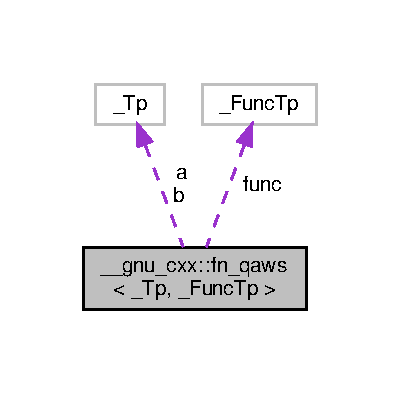
\includegraphics[width=192pt]{struct____gnu__cxx_1_1fn__qaws__coll__graph}
\end{center}
\end{figure}
\subsection*{Public Types}
\begin{DoxyCompactItemize}
\item 
using \hyperlink{struct____gnu__cxx_1_1fn__qaws_af9bc03c839ab7dc2e591b06cd3957a21}{\+\_\+\+Area\+Tp} = decltype(\hyperlink{struct____gnu__cxx_1_1fn__qaws_afb28f16c42d0f494bfe2d48e2524a5b1}{\+\_\+\+Ret\+Tp}\{\} $\ast$\hyperlink{namespace____gnu__cxx_a3b19a9c800ca194374ef9172290f7d79}{\+\_\+\+Tp}\{\})
\item 
using \hyperlink{struct____gnu__cxx_1_1fn__qaws_afb28f16c42d0f494bfe2d48e2524a5b1}{\+\_\+\+Ret\+Tp} = std\+::invoke\+\_\+result\+\_\+t$<$ \+\_\+\+Func\+Tp, \hyperlink{namespace____gnu__cxx_a3b19a9c800ca194374ef9172290f7d79}{\+\_\+\+Tp} $>$
\end{DoxyCompactItemize}
\subsection*{Public Member Functions}
\begin{DoxyCompactItemize}
\item 
\hyperlink{struct____gnu__cxx_1_1fn__qaws_a5e73b46a15a77c92f516c0ebad8a836a}{fn\+\_\+qaws} (const \hyperlink{struct____gnu__cxx_1_1qaws__integration__table}{qaws\+\_\+integration\+\_\+table}$<$ \hyperlink{namespace____gnu__cxx_a3b19a9c800ca194374ef9172290f7d79}{\+\_\+\+Tp} $>$ $\ast$\+\_\+\+\_\+tab, \+\_\+\+Func\+Tp \hyperlink{namespace____gnu__cxx_af2b2f0c7a2ae72b922b1afefae5a65b2}{\+\_\+\+\_\+func}, \hyperlink{namespace____gnu__cxx_a3b19a9c800ca194374ef9172290f7d79}{\+\_\+\+Tp} \+\_\+\+\_\+a\+\_\+in, \hyperlink{namespace____gnu__cxx_a3b19a9c800ca194374ef9172290f7d79}{\+\_\+\+Tp} \+\_\+\+\_\+b\+\_\+in)
\item 
\hyperlink{struct____gnu__cxx_1_1fn__qaws_afb28f16c42d0f494bfe2d48e2524a5b1}{\+\_\+\+Ret\+Tp} \hyperlink{struct____gnu__cxx_1_1fn__qaws_afbe290f928e148bc754398a79932386c}{eval\+\_\+left} (\hyperlink{namespace____gnu__cxx_a3b19a9c800ca194374ef9172290f7d79}{\+\_\+\+Tp}) const
\item 
\hyperlink{struct____gnu__cxx_1_1fn__qaws_afb28f16c42d0f494bfe2d48e2524a5b1}{\+\_\+\+Ret\+Tp} \hyperlink{struct____gnu__cxx_1_1fn__qaws_af2df56d9df764744fd045d26b5ef1c95}{eval\+\_\+middle} (\hyperlink{namespace____gnu__cxx_a3b19a9c800ca194374ef9172290f7d79}{\+\_\+\+Tp}) const
\item 
\hyperlink{struct____gnu__cxx_1_1fn__qaws_afb28f16c42d0f494bfe2d48e2524a5b1}{\+\_\+\+Ret\+Tp} \hyperlink{struct____gnu__cxx_1_1fn__qaws_aaace385375d3e3f74072901ea44f4b01}{eval\+\_\+right} (\hyperlink{namespace____gnu__cxx_a3b19a9c800ca194374ef9172290f7d79}{\+\_\+\+Tp}) const
\end{DoxyCompactItemize}
\subsection*{Public Attributes}
\begin{DoxyCompactItemize}
\item 
\hyperlink{namespace____gnu__cxx_a3b19a9c800ca194374ef9172290f7d79}{\+\_\+\+Tp} \hyperlink{struct____gnu__cxx_1_1fn__qaws_afe83dc1c94299aedf4cb7be0499fe572}{a}
\item 
\hyperlink{namespace____gnu__cxx_a3b19a9c800ca194374ef9172290f7d79}{\+\_\+\+Tp} \hyperlink{struct____gnu__cxx_1_1fn__qaws_a35f509512c31f2ee8fddc16405dc6e80}{b}
\item 
\+\_\+\+Func\+Tp \hyperlink{struct____gnu__cxx_1_1fn__qaws_a0fe42f7ea452aae136c5dba3264c3e93}{func}
\item 
const \hyperlink{struct____gnu__cxx_1_1qaws__integration__table}{qaws\+\_\+integration\+\_\+table}$<$ \hyperlink{namespace____gnu__cxx_a3b19a9c800ca194374ef9172290f7d79}{\+\_\+\+Tp} $>$ $\ast$ \hyperlink{struct____gnu__cxx_1_1fn__qaws_a8a96359bac745cd83938fc0735a9168d}{table}
\end{DoxyCompactItemize}


\subsection{Detailed Description}
\subsubsection*{template$<$typename \+\_\+\+Tp, typename \+\_\+\+Func\+Tp$>$\newline
struct \+\_\+\+\_\+gnu\+\_\+cxx\+::fn\+\_\+qaws$<$ \+\_\+\+Tp, \+\_\+\+Func\+Tp $>$}



Definition at line 39 of file qaws\+\_\+integrate.\+tcc.



\subsection{Member Typedef Documentation}
\mbox{\Hypertarget{struct____gnu__cxx_1_1fn__qaws_af9bc03c839ab7dc2e591b06cd3957a21}\label{struct____gnu__cxx_1_1fn__qaws_af9bc03c839ab7dc2e591b06cd3957a21}} 
\index{\+\_\+\+\_\+gnu\+\_\+cxx\+::fn\+\_\+qaws@{\+\_\+\+\_\+gnu\+\_\+cxx\+::fn\+\_\+qaws}!\+\_\+\+Area\+Tp@{\+\_\+\+Area\+Tp}}
\index{\+\_\+\+Area\+Tp@{\+\_\+\+Area\+Tp}!\+\_\+\+\_\+gnu\+\_\+cxx\+::fn\+\_\+qaws@{\+\_\+\+\_\+gnu\+\_\+cxx\+::fn\+\_\+qaws}}
\subsubsection{\texorpdfstring{\+\_\+\+Area\+Tp}{\_AreaTp}}
{\footnotesize\ttfamily template$<$typename \+\_\+\+Tp, typename \+\_\+\+Func\+Tp$>$ \\
using \hyperlink{struct____gnu__cxx_1_1fn__qaws}{\+\_\+\+\_\+gnu\+\_\+cxx\+::fn\+\_\+qaws}$<$ \hyperlink{namespace____gnu__cxx_a3b19a9c800ca194374ef9172290f7d79}{\+\_\+\+Tp}, \+\_\+\+Func\+Tp $>$\+::\hyperlink{struct____gnu__cxx_1_1fn__qaws_af9bc03c839ab7dc2e591b06cd3957a21}{\+\_\+\+Area\+Tp} =  decltype(\hyperlink{struct____gnu__cxx_1_1fn__qaws_afb28f16c42d0f494bfe2d48e2524a5b1}{\+\_\+\+Ret\+Tp}\{\} $\ast$ \hyperlink{namespace____gnu__cxx_a3b19a9c800ca194374ef9172290f7d79}{\+\_\+\+Tp}\{\})}



Definition at line 331 of file qaws\+\_\+integrate.\+tcc.

\mbox{\Hypertarget{struct____gnu__cxx_1_1fn__qaws_afb28f16c42d0f494bfe2d48e2524a5b1}\label{struct____gnu__cxx_1_1fn__qaws_afb28f16c42d0f494bfe2d48e2524a5b1}} 
\index{\+\_\+\+\_\+gnu\+\_\+cxx\+::fn\+\_\+qaws@{\+\_\+\+\_\+gnu\+\_\+cxx\+::fn\+\_\+qaws}!\+\_\+\+Ret\+Tp@{\+\_\+\+Ret\+Tp}}
\index{\+\_\+\+Ret\+Tp@{\+\_\+\+Ret\+Tp}!\+\_\+\+\_\+gnu\+\_\+cxx\+::fn\+\_\+qaws@{\+\_\+\+\_\+gnu\+\_\+cxx\+::fn\+\_\+qaws}}
\subsubsection{\texorpdfstring{\+\_\+\+Ret\+Tp}{\_RetTp}}
{\footnotesize\ttfamily template$<$typename \+\_\+\+Tp, typename \+\_\+\+Func\+Tp$>$ \\
using \hyperlink{struct____gnu__cxx_1_1fn__qaws}{\+\_\+\+\_\+gnu\+\_\+cxx\+::fn\+\_\+qaws}$<$ \hyperlink{namespace____gnu__cxx_a3b19a9c800ca194374ef9172290f7d79}{\+\_\+\+Tp}, \+\_\+\+Func\+Tp $>$\+::\hyperlink{struct____gnu__cxx_1_1fn__qaws_afb28f16c42d0f494bfe2d48e2524a5b1}{\+\_\+\+Ret\+Tp} =  std\+::invoke\+\_\+result\+\_\+t$<$\+\_\+\+Func\+Tp, \hyperlink{namespace____gnu__cxx_a3b19a9c800ca194374ef9172290f7d79}{\+\_\+\+Tp}$>$}



Definition at line 330 of file qaws\+\_\+integrate.\+tcc.



\subsection{Constructor \& Destructor Documentation}
\mbox{\Hypertarget{struct____gnu__cxx_1_1fn__qaws_a5e73b46a15a77c92f516c0ebad8a836a}\label{struct____gnu__cxx_1_1fn__qaws_a5e73b46a15a77c92f516c0ebad8a836a}} 
\index{\+\_\+\+\_\+gnu\+\_\+cxx\+::fn\+\_\+qaws@{\+\_\+\+\_\+gnu\+\_\+cxx\+::fn\+\_\+qaws}!fn\+\_\+qaws@{fn\+\_\+qaws}}
\index{fn\+\_\+qaws@{fn\+\_\+qaws}!\+\_\+\+\_\+gnu\+\_\+cxx\+::fn\+\_\+qaws@{\+\_\+\+\_\+gnu\+\_\+cxx\+::fn\+\_\+qaws}}
\subsubsection{\texorpdfstring{fn\+\_\+qaws()}{fn\_qaws()}}
{\footnotesize\ttfamily template$<$typename \+\_\+\+Tp, typename \+\_\+\+Func\+Tp$>$ \\
\hyperlink{struct____gnu__cxx_1_1fn__qaws}{\+\_\+\+\_\+gnu\+\_\+cxx\+::fn\+\_\+qaws}$<$ \hyperlink{namespace____gnu__cxx_a3b19a9c800ca194374ef9172290f7d79}{\+\_\+\+Tp}, \+\_\+\+Func\+Tp $>$\+::\hyperlink{struct____gnu__cxx_1_1fn__qaws}{fn\+\_\+qaws} (\begin{DoxyParamCaption}\item[{const \hyperlink{struct____gnu__cxx_1_1qaws__integration__table}{qaws\+\_\+integration\+\_\+table}$<$ \hyperlink{namespace____gnu__cxx_a3b19a9c800ca194374ef9172290f7d79}{\+\_\+\+Tp} $>$ $\ast$}]{\+\_\+\+\_\+tab,  }\item[{\+\_\+\+Func\+Tp}]{\+\_\+\+\_\+func,  }\item[{\hyperlink{namespace____gnu__cxx_a3b19a9c800ca194374ef9172290f7d79}{\+\_\+\+Tp}}]{\+\_\+\+\_\+a\+\_\+in,  }\item[{\hyperlink{namespace____gnu__cxx_a3b19a9c800ca194374ef9172290f7d79}{\+\_\+\+Tp}}]{\+\_\+\+\_\+b\+\_\+in }\end{DoxyParamCaption})\hspace{0.3cm}{\ttfamily [inline]}}



Definition at line 338 of file qaws\+\_\+integrate.\+tcc.


\begin{DoxyCode}
340       : \hyperlink{struct____gnu__cxx_1_1fn__qaws_a8a96359bac745cd83938fc0735a9168d}{table}(\_\_tab),
341         \hyperlink{struct____gnu__cxx_1_1fn__qaws_a0fe42f7ea452aae136c5dba3264c3e93}{func}(\hyperlink{namespace____gnu__cxx_af2b2f0c7a2ae72b922b1afefae5a65b2}{\_\_func}), \hyperlink{struct____gnu__cxx_1_1fn__qaws_afe83dc1c94299aedf4cb7be0499fe572}{a}(\_\_a\_in), \hyperlink{struct____gnu__cxx_1_1fn__qaws_a35f509512c31f2ee8fddc16405dc6e80}{b}(\_\_b\_in)
342       \{ \}
\end{DoxyCode}


\subsection{Member Function Documentation}
\mbox{\Hypertarget{struct____gnu__cxx_1_1fn__qaws_afbe290f928e148bc754398a79932386c}\label{struct____gnu__cxx_1_1fn__qaws_afbe290f928e148bc754398a79932386c}} 
\index{\+\_\+\+\_\+gnu\+\_\+cxx\+::fn\+\_\+qaws@{\+\_\+\+\_\+gnu\+\_\+cxx\+::fn\+\_\+qaws}!eval\+\_\+left@{eval\+\_\+left}}
\index{eval\+\_\+left@{eval\+\_\+left}!\+\_\+\+\_\+gnu\+\_\+cxx\+::fn\+\_\+qaws@{\+\_\+\+\_\+gnu\+\_\+cxx\+::fn\+\_\+qaws}}
\subsubsection{\texorpdfstring{eval\+\_\+left()}{eval\_left()}}
{\footnotesize\ttfamily template$<$typename \+\_\+\+Tp , typename \+\_\+\+Func\+Tp $>$ \\
std\+::invoke\+\_\+result\+\_\+t$<$ \+\_\+\+Func\+Tp, \hyperlink{namespace____gnu__cxx_a3b19a9c800ca194374ef9172290f7d79}{\+\_\+\+Tp} $>$ \hyperlink{struct____gnu__cxx_1_1fn__qaws}{\+\_\+\+\_\+gnu\+\_\+cxx\+::fn\+\_\+qaws}$<$ \hyperlink{namespace____gnu__cxx_a3b19a9c800ca194374ef9172290f7d79}{\+\_\+\+Tp}, \+\_\+\+Func\+Tp $>$\+::eval\+\_\+left (\begin{DoxyParamCaption}\item[{\hyperlink{namespace____gnu__cxx_a3b19a9c800ca194374ef9172290f7d79}{\+\_\+\+Tp}}]{\+\_\+\+\_\+x }\end{DoxyParamCaption}) const}



Definition at line 372 of file qaws\+\_\+integrate.\+tcc.



Referenced by \+\_\+\+\_\+gnu\+\_\+cxx\+::qc25s().


\begin{DoxyCode}
373     \{
374       \textcolor{keyword}{auto} \_\_factor = \hyperlink{namespace____gnu__cxx_a3b19a9c800ca194374ef9172290f7d79}{\_Tp}\{1\};
375 
376       \textcolor{keywordflow}{if} (this->\hyperlink{struct____gnu__cxx_1_1fn__qaws_a8a96359bac745cd83938fc0735a9168d}{table}->alpha != \hyperlink{namespace____gnu__cxx_a3b19a9c800ca194374ef9172290f7d79}{\_Tp}\{0\})
377         \_\_factor *= std::pow(\_\_x - this->\hyperlink{struct____gnu__cxx_1_1fn__qaws_afe83dc1c94299aedf4cb7be0499fe572}{a}, this->\hyperlink{struct____gnu__cxx_1_1fn__qaws_a8a96359bac745cd83938fc0735a9168d}{table}->alpha);
378 
379       \textcolor{keywordflow}{if} (this->\hyperlink{struct____gnu__cxx_1_1fn__qaws_a8a96359bac745cd83938fc0735a9168d}{table}->mu == 1)
380         \_\_factor *= std::log(\_\_x - this->\hyperlink{struct____gnu__cxx_1_1fn__qaws_afe83dc1c94299aedf4cb7be0499fe572}{a});
381 
382       \textcolor{keywordflow}{return} \_\_factor * this->\hyperlink{struct____gnu__cxx_1_1fn__qaws_a0fe42f7ea452aae136c5dba3264c3e93}{func}(\_\_x);
383     \}
\end{DoxyCode}
\mbox{\Hypertarget{struct____gnu__cxx_1_1fn__qaws_af2df56d9df764744fd045d26b5ef1c95}\label{struct____gnu__cxx_1_1fn__qaws_af2df56d9df764744fd045d26b5ef1c95}} 
\index{\+\_\+\+\_\+gnu\+\_\+cxx\+::fn\+\_\+qaws@{\+\_\+\+\_\+gnu\+\_\+cxx\+::fn\+\_\+qaws}!eval\+\_\+middle@{eval\+\_\+middle}}
\index{eval\+\_\+middle@{eval\+\_\+middle}!\+\_\+\+\_\+gnu\+\_\+cxx\+::fn\+\_\+qaws@{\+\_\+\+\_\+gnu\+\_\+cxx\+::fn\+\_\+qaws}}
\subsubsection{\texorpdfstring{eval\+\_\+middle()}{eval\_middle()}}
{\footnotesize\ttfamily template$<$typename \+\_\+\+Tp , typename \+\_\+\+Func\+Tp $>$ \\
std\+::invoke\+\_\+result\+\_\+t$<$ \+\_\+\+Func\+Tp, \hyperlink{namespace____gnu__cxx_a3b19a9c800ca194374ef9172290f7d79}{\+\_\+\+Tp} $>$ \hyperlink{struct____gnu__cxx_1_1fn__qaws}{\+\_\+\+\_\+gnu\+\_\+cxx\+::fn\+\_\+qaws}$<$ \hyperlink{namespace____gnu__cxx_a3b19a9c800ca194374ef9172290f7d79}{\+\_\+\+Tp}, \+\_\+\+Func\+Tp $>$\+::eval\+\_\+middle (\begin{DoxyParamCaption}\item[{\hyperlink{namespace____gnu__cxx_a3b19a9c800ca194374ef9172290f7d79}{\+\_\+\+Tp}}]{\+\_\+\+\_\+x }\end{DoxyParamCaption}) const}



Definition at line 351 of file qaws\+\_\+integrate.\+tcc.



Referenced by \+\_\+\+\_\+gnu\+\_\+cxx\+::qc25s().


\begin{DoxyCode}
352     \{
353       \textcolor{keyword}{auto} \_\_factor = \hyperlink{namespace____gnu__cxx_a3b19a9c800ca194374ef9172290f7d79}{\_Tp}\{1\};
354 
355       \textcolor{keywordflow}{if} (this->\hyperlink{struct____gnu__cxx_1_1fn__qaws_a8a96359bac745cd83938fc0735a9168d}{table}->alpha != \hyperlink{namespace____gnu__cxx_a3b19a9c800ca194374ef9172290f7d79}{\_Tp}\{0\})
356         \_\_factor *= std::pow(\_\_x - this->\hyperlink{struct____gnu__cxx_1_1fn__qaws_afe83dc1c94299aedf4cb7be0499fe572}{a}, this->\hyperlink{struct____gnu__cxx_1_1fn__qaws_a8a96359bac745cd83938fc0735a9168d}{table}->alpha);
357 
358       \textcolor{keywordflow}{if} (\hyperlink{struct____gnu__cxx_1_1fn__qaws_a8a96359bac745cd83938fc0735a9168d}{table}->mu == 1)
359         \_\_factor *= std::log(\_\_x - this->\hyperlink{struct____gnu__cxx_1_1fn__qaws_afe83dc1c94299aedf4cb7be0499fe572}{a});
360 
361       \textcolor{keywordflow}{if} (this->\hyperlink{struct____gnu__cxx_1_1fn__qaws_a8a96359bac745cd83938fc0735a9168d}{table}->beta != \hyperlink{namespace____gnu__cxx_a3b19a9c800ca194374ef9172290f7d79}{\_Tp}\{0\})
362         \_\_factor *= std::pow(this->\hyperlink{struct____gnu__cxx_1_1fn__qaws_a35f509512c31f2ee8fddc16405dc6e80}{b} - \_\_x, this->\hyperlink{struct____gnu__cxx_1_1fn__qaws_a8a96359bac745cd83938fc0735a9168d}{table}->beta);
363 
364       \textcolor{keywordflow}{if} (\hyperlink{struct____gnu__cxx_1_1fn__qaws_a8a96359bac745cd83938fc0735a9168d}{table}->nu == 1)
365         \_\_factor *= std::log(this->\hyperlink{struct____gnu__cxx_1_1fn__qaws_a35f509512c31f2ee8fddc16405dc6e80}{b} - \_\_x);
366 
367       \textcolor{keywordflow}{return} \_\_factor * this->\hyperlink{struct____gnu__cxx_1_1fn__qaws_a0fe42f7ea452aae136c5dba3264c3e93}{func}(\_\_x);
368     \}
\end{DoxyCode}
\mbox{\Hypertarget{struct____gnu__cxx_1_1fn__qaws_aaace385375d3e3f74072901ea44f4b01}\label{struct____gnu__cxx_1_1fn__qaws_aaace385375d3e3f74072901ea44f4b01}} 
\index{\+\_\+\+\_\+gnu\+\_\+cxx\+::fn\+\_\+qaws@{\+\_\+\+\_\+gnu\+\_\+cxx\+::fn\+\_\+qaws}!eval\+\_\+right@{eval\+\_\+right}}
\index{eval\+\_\+right@{eval\+\_\+right}!\+\_\+\+\_\+gnu\+\_\+cxx\+::fn\+\_\+qaws@{\+\_\+\+\_\+gnu\+\_\+cxx\+::fn\+\_\+qaws}}
\subsubsection{\texorpdfstring{eval\+\_\+right()}{eval\_right()}}
{\footnotesize\ttfamily template$<$typename \+\_\+\+Tp , typename \+\_\+\+Func\+Tp $>$ \\
std\+::invoke\+\_\+result\+\_\+t$<$ \+\_\+\+Func\+Tp, \hyperlink{namespace____gnu__cxx_a3b19a9c800ca194374ef9172290f7d79}{\+\_\+\+Tp} $>$ \hyperlink{struct____gnu__cxx_1_1fn__qaws}{\+\_\+\+\_\+gnu\+\_\+cxx\+::fn\+\_\+qaws}$<$ \hyperlink{namespace____gnu__cxx_a3b19a9c800ca194374ef9172290f7d79}{\+\_\+\+Tp}, \+\_\+\+Func\+Tp $>$\+::eval\+\_\+right (\begin{DoxyParamCaption}\item[{\hyperlink{namespace____gnu__cxx_a3b19a9c800ca194374ef9172290f7d79}{\+\_\+\+Tp}}]{\+\_\+\+\_\+x }\end{DoxyParamCaption}) const}



Definition at line 387 of file qaws\+\_\+integrate.\+tcc.



References \+\_\+\+\_\+gnu\+\_\+cxx\+::compute\+\_\+result\+\_\+t$<$ \+\_\+\+Area\+Tp $>$\+::\+\_\+\+\_\+res12, \+\_\+\+\_\+gnu\+\_\+cxx\+::compute\+\_\+result\+\_\+t$<$ \+\_\+\+Area\+Tp $>$\+::\+\_\+\+\_\+res24, and \+\_\+\+\_\+gnu\+\_\+cxx\+::compute\+\_\+result().



Referenced by \+\_\+\+\_\+gnu\+\_\+cxx\+::qc25s().


\begin{DoxyCode}
388     \{
389       \textcolor{keyword}{auto} \_\_factor = \hyperlink{namespace____gnu__cxx_a3b19a9c800ca194374ef9172290f7d79}{\_Tp}\{1\};
390 
391       \textcolor{keywordflow}{if} (this->\hyperlink{struct____gnu__cxx_1_1fn__qaws_a8a96359bac745cd83938fc0735a9168d}{table}->beta != \hyperlink{namespace____gnu__cxx_a3b19a9c800ca194374ef9172290f7d79}{\_Tp}\{0\})
392         \_\_factor *= std::pow(this->\hyperlink{struct____gnu__cxx_1_1fn__qaws_a35f509512c31f2ee8fddc16405dc6e80}{b} - \_\_x, this->\hyperlink{struct____gnu__cxx_1_1fn__qaws_a8a96359bac745cd83938fc0735a9168d}{table}->beta);
393 
394       \textcolor{keywordflow}{if} (this->\hyperlink{struct____gnu__cxx_1_1fn__qaws_a8a96359bac745cd83938fc0735a9168d}{table}->nu == 1)
395         \_\_factor *= std::log(this->\hyperlink{struct____gnu__cxx_1_1fn__qaws_a35f509512c31f2ee8fddc16405dc6e80}{b} - \_\_x);
396 
397       \textcolor{keywordflow}{return} \_\_factor * this->\hyperlink{struct____gnu__cxx_1_1fn__qaws_a0fe42f7ea452aae136c5dba3264c3e93}{func}(\_\_x);
398     \}
\end{DoxyCode}


\subsection{Member Data Documentation}
\mbox{\Hypertarget{struct____gnu__cxx_1_1fn__qaws_afe83dc1c94299aedf4cb7be0499fe572}\label{struct____gnu__cxx_1_1fn__qaws_afe83dc1c94299aedf4cb7be0499fe572}} 
\index{\+\_\+\+\_\+gnu\+\_\+cxx\+::fn\+\_\+qaws@{\+\_\+\+\_\+gnu\+\_\+cxx\+::fn\+\_\+qaws}!a@{a}}
\index{a@{a}!\+\_\+\+\_\+gnu\+\_\+cxx\+::fn\+\_\+qaws@{\+\_\+\+\_\+gnu\+\_\+cxx\+::fn\+\_\+qaws}}
\subsubsection{\texorpdfstring{a}{a}}
{\footnotesize\ttfamily template$<$typename \+\_\+\+Tp, typename \+\_\+\+Func\+Tp$>$ \\
\hyperlink{namespace____gnu__cxx_a3b19a9c800ca194374ef9172290f7d79}{\+\_\+\+Tp} \hyperlink{struct____gnu__cxx_1_1fn__qaws}{\+\_\+\+\_\+gnu\+\_\+cxx\+::fn\+\_\+qaws}$<$ \hyperlink{namespace____gnu__cxx_a3b19a9c800ca194374ef9172290f7d79}{\+\_\+\+Tp}, \+\_\+\+Func\+Tp $>$\+::a}



Definition at line 335 of file qaws\+\_\+integrate.\+tcc.

\mbox{\Hypertarget{struct____gnu__cxx_1_1fn__qaws_a35f509512c31f2ee8fddc16405dc6e80}\label{struct____gnu__cxx_1_1fn__qaws_a35f509512c31f2ee8fddc16405dc6e80}} 
\index{\+\_\+\+\_\+gnu\+\_\+cxx\+::fn\+\_\+qaws@{\+\_\+\+\_\+gnu\+\_\+cxx\+::fn\+\_\+qaws}!b@{b}}
\index{b@{b}!\+\_\+\+\_\+gnu\+\_\+cxx\+::fn\+\_\+qaws@{\+\_\+\+\_\+gnu\+\_\+cxx\+::fn\+\_\+qaws}}
\subsubsection{\texorpdfstring{b}{b}}
{\footnotesize\ttfamily template$<$typename \+\_\+\+Tp, typename \+\_\+\+Func\+Tp$>$ \\
\hyperlink{namespace____gnu__cxx_a3b19a9c800ca194374ef9172290f7d79}{\+\_\+\+Tp} \hyperlink{struct____gnu__cxx_1_1fn__qaws}{\+\_\+\+\_\+gnu\+\_\+cxx\+::fn\+\_\+qaws}$<$ \hyperlink{namespace____gnu__cxx_a3b19a9c800ca194374ef9172290f7d79}{\+\_\+\+Tp}, \+\_\+\+Func\+Tp $>$\+::b}



Definition at line 336 of file qaws\+\_\+integrate.\+tcc.

\mbox{\Hypertarget{struct____gnu__cxx_1_1fn__qaws_a0fe42f7ea452aae136c5dba3264c3e93}\label{struct____gnu__cxx_1_1fn__qaws_a0fe42f7ea452aae136c5dba3264c3e93}} 
\index{\+\_\+\+\_\+gnu\+\_\+cxx\+::fn\+\_\+qaws@{\+\_\+\+\_\+gnu\+\_\+cxx\+::fn\+\_\+qaws}!func@{func}}
\index{func@{func}!\+\_\+\+\_\+gnu\+\_\+cxx\+::fn\+\_\+qaws@{\+\_\+\+\_\+gnu\+\_\+cxx\+::fn\+\_\+qaws}}
\subsubsection{\texorpdfstring{func}{func}}
{\footnotesize\ttfamily template$<$typename \+\_\+\+Tp, typename \+\_\+\+Func\+Tp$>$ \\
\+\_\+\+Func\+Tp \hyperlink{struct____gnu__cxx_1_1fn__qaws}{\+\_\+\+\_\+gnu\+\_\+cxx\+::fn\+\_\+qaws}$<$ \hyperlink{namespace____gnu__cxx_a3b19a9c800ca194374ef9172290f7d79}{\+\_\+\+Tp}, \+\_\+\+Func\+Tp $>$\+::func}



Definition at line 334 of file qaws\+\_\+integrate.\+tcc.

\mbox{\Hypertarget{struct____gnu__cxx_1_1fn__qaws_a8a96359bac745cd83938fc0735a9168d}\label{struct____gnu__cxx_1_1fn__qaws_a8a96359bac745cd83938fc0735a9168d}} 
\index{\+\_\+\+\_\+gnu\+\_\+cxx\+::fn\+\_\+qaws@{\+\_\+\+\_\+gnu\+\_\+cxx\+::fn\+\_\+qaws}!table@{table}}
\index{table@{table}!\+\_\+\+\_\+gnu\+\_\+cxx\+::fn\+\_\+qaws@{\+\_\+\+\_\+gnu\+\_\+cxx\+::fn\+\_\+qaws}}
\subsubsection{\texorpdfstring{table}{table}}
{\footnotesize\ttfamily template$<$typename \+\_\+\+Tp, typename \+\_\+\+Func\+Tp$>$ \\
const \hyperlink{struct____gnu__cxx_1_1qaws__integration__table}{qaws\+\_\+integration\+\_\+table}$<$\hyperlink{namespace____gnu__cxx_a3b19a9c800ca194374ef9172290f7d79}{\+\_\+\+Tp}$>$$\ast$ \hyperlink{struct____gnu__cxx_1_1fn__qaws}{\+\_\+\+\_\+gnu\+\_\+cxx\+::fn\+\_\+qaws}$<$ \hyperlink{namespace____gnu__cxx_a3b19a9c800ca194374ef9172290f7d79}{\+\_\+\+Tp}, \+\_\+\+Func\+Tp $>$\+::table}



Definition at line 333 of file qaws\+\_\+integrate.\+tcc.



The documentation for this struct was generated from the following file\+:\begin{DoxyCompactItemize}
\item 
include/ext/\hyperlink{qaws__integrate_8tcc}{qaws\+\_\+integrate.\+tcc}\end{DoxyCompactItemize}

\hypertarget{class____gnu__cxx_1_1fourier__transform__t}{}\section{\+\_\+\+\_\+gnu\+\_\+cxx\+:\+:fourier\+\_\+transform\+\_\+t$<$ \+\_\+\+Tp $>$ Class Template Reference}
\label{class____gnu__cxx_1_1fourier__transform__t}\index{\+\_\+\+\_\+gnu\+\_\+cxx\+::fourier\+\_\+transform\+\_\+t$<$ \+\_\+\+Tp $>$@{\+\_\+\+\_\+gnu\+\_\+cxx\+::fourier\+\_\+transform\+\_\+t$<$ \+\_\+\+Tp $>$}}


{\ttfamily \#include $<$fourier\+\_\+transform.\+h$>$}

\subsection*{Public Member Functions}
\begin{DoxyCompactItemize}
\item 
\hyperlink{class____gnu__cxx_1_1fourier__transform__t_ae9d6b51de92d52ba301457c4a9680a64}{fourier\+\_\+transform\+\_\+t} (std\+::size\+\_\+t \+\_\+\+\_\+n)
\item 
\hyperlink{class____gnu__cxx_1_1fourier__transform__t_abb69842c2d297492cc5cd22e4b0ee34e}{fourier\+\_\+transform\+\_\+t} (std\+::vector$<$ \hyperlink{namespace____gnu__cxx_a3b19a9c800ca194374ef9172290f7d79}{\+\_\+\+Tp} $>$ \+\_\+\+\_\+data)
\item 
std\+::complex$<$ \hyperlink{namespace____gnu__cxx_a3b19a9c800ca194374ef9172290f7d79}{\+\_\+\+Tp} $>$ \hyperlink{class____gnu__cxx_1_1fourier__transform__t_a1b39e5c1042bdb5b60d4f833d5661ed8}{operator\mbox{[}$\,$\mbox{]}} (std\+::size\+\_\+t \+\_\+\+\_\+k) const
\item 
std\+::size\+\_\+t \hyperlink{class____gnu__cxx_1_1fourier__transform__t_a667f8cb207f9d8e4c8643fe0bf165ff4}{size} () const
\end{DoxyCompactItemize}


\subsection{Detailed Description}
\subsubsection*{template$<$typename \+\_\+\+Tp$>$\newline
class \+\_\+\+\_\+gnu\+\_\+cxx\+::fourier\+\_\+transform\+\_\+t$<$ \+\_\+\+Tp $>$}

Fast Fourier Transform

Discrete Fourier Transform can be regarded as evaluating a polynomial of degree N-\/1 on the powers $ \omega^0, \omega, \omega^2, ..., \omega^(N-1) $ where $ \omega $ is the Nth root of unity.

Given a polynomial of even degree \[ p(t) = a_0 + a_1 t + a_2 t^2 + ... \] we find\+: \[ p(t) = a_0 + a_2 t^2 + a_4 t^4 + ... + t(a_1 + a_3 t^2 + ...) = q_{even}(t^2) + t q_{odd} (t^2) \] where q\+\_\+e and q\+\_\+o are polynomials formed with the even and odd coefficients of p(t). Thus, we get

p(1) = q\+\_\+\{even\}(1) + $^\wedge$0 q\+\_\+\{odd\}(1) p() = q\+\_\+\{even\}($^\wedge$2) + $^\wedge$1 q\+\_\+\{odd\}($^\wedge$2) p($^\wedge$2) = q\+\_\+\{even\}($^\wedge$4) + $^\wedge$2 q\+\_\+\{odd\}($^\wedge$4) ...

Note how on the R\+HS the Fourier transforms of q\+\_\+e and q\+\_\+o appear. Thus\+: Discrete Fourier transform type. 

Definition at line 153 of file fourier\+\_\+transform.\+h.



\subsection{Constructor \& Destructor Documentation}
\mbox{\Hypertarget{class____gnu__cxx_1_1fourier__transform__t_ae9d6b51de92d52ba301457c4a9680a64}\label{class____gnu__cxx_1_1fourier__transform__t_ae9d6b51de92d52ba301457c4a9680a64}} 
\index{\+\_\+\+\_\+gnu\+\_\+cxx\+::fourier\+\_\+transform\+\_\+t@{\+\_\+\+\_\+gnu\+\_\+cxx\+::fourier\+\_\+transform\+\_\+t}!fourier\+\_\+transform\+\_\+t@{fourier\+\_\+transform\+\_\+t}}
\index{fourier\+\_\+transform\+\_\+t@{fourier\+\_\+transform\+\_\+t}!\+\_\+\+\_\+gnu\+\_\+cxx\+::fourier\+\_\+transform\+\_\+t@{\+\_\+\+\_\+gnu\+\_\+cxx\+::fourier\+\_\+transform\+\_\+t}}
\subsubsection{\texorpdfstring{fourier\+\_\+transform\+\_\+t()}{fourier\_transform\_t()}\hspace{0.1cm}{\footnotesize\ttfamily [1/2]}}
{\footnotesize\ttfamily template$<$typename \+\_\+\+Tp $>$ \\
\hyperlink{class____gnu__cxx_1_1fourier__transform__t}{\+\_\+\+\_\+gnu\+\_\+cxx\+::fourier\+\_\+transform\+\_\+t}$<$ \hyperlink{namespace____gnu__cxx_a3b19a9c800ca194374ef9172290f7d79}{\+\_\+\+Tp} $>$\+::\hyperlink{class____gnu__cxx_1_1fourier__transform__t}{fourier\+\_\+transform\+\_\+t} (\begin{DoxyParamCaption}\item[{std\+::size\+\_\+t}]{\+\_\+\+\_\+n }\end{DoxyParamCaption})\hspace{0.3cm}{\ttfamily [inline]}}



Definition at line 161 of file fourier\+\_\+transform.\+h.


\begin{DoxyCode}
162       : \_M\_xform\{\}
163       \{ this->\_M\_xform.reserve(\_\_n / 2 + 1); \}
\end{DoxyCode}
\mbox{\Hypertarget{class____gnu__cxx_1_1fourier__transform__t_abb69842c2d297492cc5cd22e4b0ee34e}\label{class____gnu__cxx_1_1fourier__transform__t_abb69842c2d297492cc5cd22e4b0ee34e}} 
\index{\+\_\+\+\_\+gnu\+\_\+cxx\+::fourier\+\_\+transform\+\_\+t@{\+\_\+\+\_\+gnu\+\_\+cxx\+::fourier\+\_\+transform\+\_\+t}!fourier\+\_\+transform\+\_\+t@{fourier\+\_\+transform\+\_\+t}}
\index{fourier\+\_\+transform\+\_\+t@{fourier\+\_\+transform\+\_\+t}!\+\_\+\+\_\+gnu\+\_\+cxx\+::fourier\+\_\+transform\+\_\+t@{\+\_\+\+\_\+gnu\+\_\+cxx\+::fourier\+\_\+transform\+\_\+t}}
\subsubsection{\texorpdfstring{fourier\+\_\+transform\+\_\+t()}{fourier\_transform\_t()}\hspace{0.1cm}{\footnotesize\ttfamily [2/2]}}
{\footnotesize\ttfamily template$<$typename \+\_\+\+Tp $>$ \\
\hyperlink{class____gnu__cxx_1_1fourier__transform__t}{\+\_\+\+\_\+gnu\+\_\+cxx\+::fourier\+\_\+transform\+\_\+t}$<$ \hyperlink{namespace____gnu__cxx_a3b19a9c800ca194374ef9172290f7d79}{\+\_\+\+Tp} $>$\+::\hyperlink{class____gnu__cxx_1_1fourier__transform__t}{fourier\+\_\+transform\+\_\+t} (\begin{DoxyParamCaption}\item[{std\+::vector$<$ \hyperlink{namespace____gnu__cxx_a3b19a9c800ca194374ef9172290f7d79}{\+\_\+\+Tp} $>$}]{\+\_\+\+\_\+data }\end{DoxyParamCaption})}



\subsection{Member Function Documentation}
\mbox{\Hypertarget{class____gnu__cxx_1_1fourier__transform__t_a1b39e5c1042bdb5b60d4f833d5661ed8}\label{class____gnu__cxx_1_1fourier__transform__t_a1b39e5c1042bdb5b60d4f833d5661ed8}} 
\index{\+\_\+\+\_\+gnu\+\_\+cxx\+::fourier\+\_\+transform\+\_\+t@{\+\_\+\+\_\+gnu\+\_\+cxx\+::fourier\+\_\+transform\+\_\+t}!operator\mbox{[}\mbox{]}@{operator[]}}
\index{operator\mbox{[}\mbox{]}@{operator[]}!\+\_\+\+\_\+gnu\+\_\+cxx\+::fourier\+\_\+transform\+\_\+t@{\+\_\+\+\_\+gnu\+\_\+cxx\+::fourier\+\_\+transform\+\_\+t}}
\subsubsection{\texorpdfstring{operator[]()}{operator[]()}}
{\footnotesize\ttfamily template$<$typename \+\_\+\+Tp $>$ \\
std\+::complex$<$\hyperlink{namespace____gnu__cxx_a3b19a9c800ca194374ef9172290f7d79}{\+\_\+\+Tp}$>$ \hyperlink{class____gnu__cxx_1_1fourier__transform__t}{\+\_\+\+\_\+gnu\+\_\+cxx\+::fourier\+\_\+transform\+\_\+t}$<$ \hyperlink{namespace____gnu__cxx_a3b19a9c800ca194374ef9172290f7d79}{\+\_\+\+Tp} $>$\+::operator\mbox{[}$\,$\mbox{]} (\begin{DoxyParamCaption}\item[{std\+::size\+\_\+t}]{\+\_\+\+\_\+k }\end{DoxyParamCaption}) const\hspace{0.3cm}{\ttfamily [inline]}}



Definition at line 172 of file fourier\+\_\+transform.\+h.


\begin{DoxyCode}
173       \{
174         \textcolor{keywordflow}{if} (\_\_k < this->\_M\_xform.size())
175           \textcolor{keywordflow}{return} this->\_M\_xform[\_\_k];
176         \textcolor{keywordflow}{else}
177           \textcolor{keywordflow}{return} std::conj(this->\_M\_xform[this->\_M\_xform.size() - \_\_k]);
178         \textcolor{comment}{// This is real array indexing.}
179         \textcolor{comment}{//if (\_\_k < len / 2)}
180         \textcolor{comment}{//      ? std::complex(xform[2 * \_\_k], xform[2 * \_\_k + 1])}
181         \textcolor{comment}{//      : std::complex(xform[2 * len - 2 * i - 2],}
182         \textcolor{comment}{//                    -xform[2 * len - 2 * \_\_k - 1]);}
183       \}
\end{DoxyCode}
\mbox{\Hypertarget{class____gnu__cxx_1_1fourier__transform__t_a667f8cb207f9d8e4c8643fe0bf165ff4}\label{class____gnu__cxx_1_1fourier__transform__t_a667f8cb207f9d8e4c8643fe0bf165ff4}} 
\index{\+\_\+\+\_\+gnu\+\_\+cxx\+::fourier\+\_\+transform\+\_\+t@{\+\_\+\+\_\+gnu\+\_\+cxx\+::fourier\+\_\+transform\+\_\+t}!size@{size}}
\index{size@{size}!\+\_\+\+\_\+gnu\+\_\+cxx\+::fourier\+\_\+transform\+\_\+t@{\+\_\+\+\_\+gnu\+\_\+cxx\+::fourier\+\_\+transform\+\_\+t}}
\subsubsection{\texorpdfstring{size()}{size()}}
{\footnotesize\ttfamily template$<$typename \+\_\+\+Tp $>$ \\
std\+::size\+\_\+t \hyperlink{class____gnu__cxx_1_1fourier__transform__t}{\+\_\+\+\_\+gnu\+\_\+cxx\+::fourier\+\_\+transform\+\_\+t}$<$ \hyperlink{namespace____gnu__cxx_a3b19a9c800ca194374ef9172290f7d79}{\+\_\+\+Tp} $>$\+::size (\begin{DoxyParamCaption}{ }\end{DoxyParamCaption}) const\hspace{0.3cm}{\ttfamily [inline]}}



Definition at line 168 of file fourier\+\_\+transform.\+h.


\begin{DoxyCode}
169       \{ \textcolor{keywordflow}{return} 2 * this->\_M\_xform.size() - 2; \}
\end{DoxyCode}


The documentation for this class was generated from the following file\+:\begin{DoxyCompactItemize}
\item 
include/ext/\hyperlink{fourier__transform_8h}{fourier\+\_\+transform.\+h}\end{DoxyCompactItemize}

\hypertarget{class____gnu__cxx_1_1fourier__transform__t_3_01std_1_1complex_3_01__Tp_01_4_01_4}{}\section{\+\_\+\+\_\+gnu\+\_\+cxx\+:\+:fourier\+\_\+transform\+\_\+t$<$ std\+:\+:complex$<$ \+\_\+\+Tp $>$ $>$ Class Template Reference}
\label{class____gnu__cxx_1_1fourier__transform__t_3_01std_1_1complex_3_01__Tp_01_4_01_4}\index{\+\_\+\+\_\+gnu\+\_\+cxx\+::fourier\+\_\+transform\+\_\+t$<$ std\+::complex$<$ \+\_\+\+Tp $>$ $>$@{\+\_\+\+\_\+gnu\+\_\+cxx\+::fourier\+\_\+transform\+\_\+t$<$ std\+::complex$<$ \+\_\+\+Tp $>$ $>$}}


{\ttfamily \#include $<$fourier\+\_\+transform.\+h$>$}

\subsection*{Public Member Functions}
\begin{DoxyCompactItemize}
\item 
\hyperlink{class____gnu__cxx_1_1fourier__transform__t_3_01std_1_1complex_3_01__Tp_01_4_01_4_a215f06e5944b3666d4bd737154625317}{fourier\+\_\+transform\+\_\+t} (std\+::size\+\_\+t \+\_\+\+\_\+n)
\item 
\hyperlink{class____gnu__cxx_1_1fourier__transform__t_3_01std_1_1complex_3_01__Tp_01_4_01_4_a16c7b15061a8a9038df61d009def6ee1}{fourier\+\_\+transform\+\_\+t} (const std\+::vector$<$ std\+::complex$<$ \hyperlink{namespace____gnu__cxx_a3b19a9c800ca194374ef9172290f7d79}{\+\_\+\+Tp} $>$$>$ \&\+\_\+\+\_\+data)
\item 
std\+::complex$<$ \hyperlink{namespace____gnu__cxx_a3b19a9c800ca194374ef9172290f7d79}{\+\_\+\+Tp} $>$ \hyperlink{class____gnu__cxx_1_1fourier__transform__t_3_01std_1_1complex_3_01__Tp_01_4_01_4_aab8999adeedcd40323a2e3ee29531b24}{operator\mbox{[}$\,$\mbox{]}} (std\+::size\+\_\+t \+\_\+\+\_\+k) const
\item 
std\+::size\+\_\+t \hyperlink{class____gnu__cxx_1_1fourier__transform__t_3_01std_1_1complex_3_01__Tp_01_4_01_4_a1c6e363c86ed959497fd6ad5866802d6}{size} () const
\end{DoxyCompactItemize}


\subsection{Detailed Description}
\subsubsection*{template$<$typename \+\_\+\+Tp$>$\newline
class \+\_\+\+\_\+gnu\+\_\+cxx\+::fourier\+\_\+transform\+\_\+t$<$ std\+::complex$<$ \+\_\+\+Tp $>$ $>$}

Discrete Fourier transform specialization for transform of complex data. 

Definition at line 190 of file fourier\+\_\+transform.\+h.



\subsection{Constructor \& Destructor Documentation}
\mbox{\Hypertarget{class____gnu__cxx_1_1fourier__transform__t_3_01std_1_1complex_3_01__Tp_01_4_01_4_a215f06e5944b3666d4bd737154625317}\label{class____gnu__cxx_1_1fourier__transform__t_3_01std_1_1complex_3_01__Tp_01_4_01_4_a215f06e5944b3666d4bd737154625317}} 
\index{\+\_\+\+\_\+gnu\+\_\+cxx\+::fourier\+\_\+transform\+\_\+t$<$ std\+::complex$<$ \+\_\+\+Tp $>$ $>$@{\+\_\+\+\_\+gnu\+\_\+cxx\+::fourier\+\_\+transform\+\_\+t$<$ std\+::complex$<$ \+\_\+\+Tp $>$ $>$}!fourier\+\_\+transform\+\_\+t@{fourier\+\_\+transform\+\_\+t}}
\index{fourier\+\_\+transform\+\_\+t@{fourier\+\_\+transform\+\_\+t}!\+\_\+\+\_\+gnu\+\_\+cxx\+::fourier\+\_\+transform\+\_\+t$<$ std\+::complex$<$ \+\_\+\+Tp $>$ $>$@{\+\_\+\+\_\+gnu\+\_\+cxx\+::fourier\+\_\+transform\+\_\+t$<$ std\+::complex$<$ \+\_\+\+Tp $>$ $>$}}
\subsubsection{\texorpdfstring{fourier\+\_\+transform\+\_\+t()}{fourier\_transform\_t()}\hspace{0.1cm}{\footnotesize\ttfamily [1/2]}}
{\footnotesize\ttfamily template$<$typename \+\_\+\+Tp $>$ \\
\hyperlink{class____gnu__cxx_1_1fourier__transform__t}{\+\_\+\+\_\+gnu\+\_\+cxx\+::fourier\+\_\+transform\+\_\+t}$<$ std\+::complex$<$ \hyperlink{namespace____gnu__cxx_a3b19a9c800ca194374ef9172290f7d79}{\+\_\+\+Tp} $>$ $>$\+::\hyperlink{class____gnu__cxx_1_1fourier__transform__t}{fourier\+\_\+transform\+\_\+t} (\begin{DoxyParamCaption}\item[{std\+::size\+\_\+t}]{\+\_\+\+\_\+n }\end{DoxyParamCaption})\hspace{0.3cm}{\ttfamily [inline]}}



Definition at line 198 of file fourier\+\_\+transform.\+h.


\begin{DoxyCode}
199       : \_M\_xform\{\}
200       \{ this->\_M\_xform.reserve(\_\_n / 2 + 1); \}
\end{DoxyCode}
\mbox{\Hypertarget{class____gnu__cxx_1_1fourier__transform__t_3_01std_1_1complex_3_01__Tp_01_4_01_4_a16c7b15061a8a9038df61d009def6ee1}\label{class____gnu__cxx_1_1fourier__transform__t_3_01std_1_1complex_3_01__Tp_01_4_01_4_a16c7b15061a8a9038df61d009def6ee1}} 
\index{\+\_\+\+\_\+gnu\+\_\+cxx\+::fourier\+\_\+transform\+\_\+t$<$ std\+::complex$<$ \+\_\+\+Tp $>$ $>$@{\+\_\+\+\_\+gnu\+\_\+cxx\+::fourier\+\_\+transform\+\_\+t$<$ std\+::complex$<$ \+\_\+\+Tp $>$ $>$}!fourier\+\_\+transform\+\_\+t@{fourier\+\_\+transform\+\_\+t}}
\index{fourier\+\_\+transform\+\_\+t@{fourier\+\_\+transform\+\_\+t}!\+\_\+\+\_\+gnu\+\_\+cxx\+::fourier\+\_\+transform\+\_\+t$<$ std\+::complex$<$ \+\_\+\+Tp $>$ $>$@{\+\_\+\+\_\+gnu\+\_\+cxx\+::fourier\+\_\+transform\+\_\+t$<$ std\+::complex$<$ \+\_\+\+Tp $>$ $>$}}
\subsubsection{\texorpdfstring{fourier\+\_\+transform\+\_\+t()}{fourier\_transform\_t()}\hspace{0.1cm}{\footnotesize\ttfamily [2/2]}}
{\footnotesize\ttfamily template$<$typename \+\_\+\+Tp $>$ \\
\hyperlink{class____gnu__cxx_1_1fourier__transform__t}{\+\_\+\+\_\+gnu\+\_\+cxx\+::fourier\+\_\+transform\+\_\+t}$<$ std\+::complex$<$ \hyperlink{namespace____gnu__cxx_a3b19a9c800ca194374ef9172290f7d79}{\+\_\+\+Tp} $>$ $>$\+::\hyperlink{class____gnu__cxx_1_1fourier__transform__t}{fourier\+\_\+transform\+\_\+t} (\begin{DoxyParamCaption}\item[{const std\+::vector$<$ std\+::complex$<$ \hyperlink{namespace____gnu__cxx_a3b19a9c800ca194374ef9172290f7d79}{\+\_\+\+Tp} $>$$>$ \&}]{\+\_\+\+\_\+data }\end{DoxyParamCaption})}



\subsection{Member Function Documentation}
\mbox{\Hypertarget{class____gnu__cxx_1_1fourier__transform__t_3_01std_1_1complex_3_01__Tp_01_4_01_4_aab8999adeedcd40323a2e3ee29531b24}\label{class____gnu__cxx_1_1fourier__transform__t_3_01std_1_1complex_3_01__Tp_01_4_01_4_aab8999adeedcd40323a2e3ee29531b24}} 
\index{\+\_\+\+\_\+gnu\+\_\+cxx\+::fourier\+\_\+transform\+\_\+t$<$ std\+::complex$<$ \+\_\+\+Tp $>$ $>$@{\+\_\+\+\_\+gnu\+\_\+cxx\+::fourier\+\_\+transform\+\_\+t$<$ std\+::complex$<$ \+\_\+\+Tp $>$ $>$}!operator\mbox{[}\mbox{]}@{operator[]}}
\index{operator\mbox{[}\mbox{]}@{operator[]}!\+\_\+\+\_\+gnu\+\_\+cxx\+::fourier\+\_\+transform\+\_\+t$<$ std\+::complex$<$ \+\_\+\+Tp $>$ $>$@{\+\_\+\+\_\+gnu\+\_\+cxx\+::fourier\+\_\+transform\+\_\+t$<$ std\+::complex$<$ \+\_\+\+Tp $>$ $>$}}
\subsubsection{\texorpdfstring{operator[]()}{operator[]()}}
{\footnotesize\ttfamily template$<$typename \+\_\+\+Tp $>$ \\
std\+::complex$<$\hyperlink{namespace____gnu__cxx_a3b19a9c800ca194374ef9172290f7d79}{\+\_\+\+Tp}$>$ \hyperlink{class____gnu__cxx_1_1fourier__transform__t}{\+\_\+\+\_\+gnu\+\_\+cxx\+::fourier\+\_\+transform\+\_\+t}$<$ std\+::complex$<$ \hyperlink{namespace____gnu__cxx_a3b19a9c800ca194374ef9172290f7d79}{\+\_\+\+Tp} $>$ $>$\+::operator\mbox{[}$\,$\mbox{]} (\begin{DoxyParamCaption}\item[{std\+::size\+\_\+t}]{\+\_\+\+\_\+k }\end{DoxyParamCaption}) const\hspace{0.3cm}{\ttfamily [inline]}}



Definition at line 209 of file fourier\+\_\+transform.\+h.



References \+\_\+\+\_\+gnu\+\_\+cxx\+::\+\_\+\+\_\+discrete\+\_\+fourier\+\_\+transform(), \+\_\+\+\_\+gnu\+\_\+cxx\+::fast\+\_\+fourier\+\_\+transform(), \+\_\+\+\_\+gnu\+\_\+cxx\+::fast\+\_\+sine\+\_\+transform(), \+\_\+\+\_\+gnu\+\_\+cxx\+::inv\+\_\+fast\+\_\+fourier\+\_\+transform(), and \+\_\+\+\_\+gnu\+\_\+cxx\+::inv\+\_\+fast\+\_\+sine\+\_\+transform().


\begin{DoxyCode}
210       \{ \textcolor{keywordflow}{return} this->\_M\_xform[\_\_k]; \}
\end{DoxyCode}
\mbox{\Hypertarget{class____gnu__cxx_1_1fourier__transform__t_3_01std_1_1complex_3_01__Tp_01_4_01_4_a1c6e363c86ed959497fd6ad5866802d6}\label{class____gnu__cxx_1_1fourier__transform__t_3_01std_1_1complex_3_01__Tp_01_4_01_4_a1c6e363c86ed959497fd6ad5866802d6}} 
\index{\+\_\+\+\_\+gnu\+\_\+cxx\+::fourier\+\_\+transform\+\_\+t$<$ std\+::complex$<$ \+\_\+\+Tp $>$ $>$@{\+\_\+\+\_\+gnu\+\_\+cxx\+::fourier\+\_\+transform\+\_\+t$<$ std\+::complex$<$ \+\_\+\+Tp $>$ $>$}!size@{size}}
\index{size@{size}!\+\_\+\+\_\+gnu\+\_\+cxx\+::fourier\+\_\+transform\+\_\+t$<$ std\+::complex$<$ \+\_\+\+Tp $>$ $>$@{\+\_\+\+\_\+gnu\+\_\+cxx\+::fourier\+\_\+transform\+\_\+t$<$ std\+::complex$<$ \+\_\+\+Tp $>$ $>$}}
\subsubsection{\texorpdfstring{size()}{size()}}
{\footnotesize\ttfamily template$<$typename \+\_\+\+Tp $>$ \\
std\+::size\+\_\+t \hyperlink{class____gnu__cxx_1_1fourier__transform__t}{\+\_\+\+\_\+gnu\+\_\+cxx\+::fourier\+\_\+transform\+\_\+t}$<$ std\+::complex$<$ \hyperlink{namespace____gnu__cxx_a3b19a9c800ca194374ef9172290f7d79}{\+\_\+\+Tp} $>$ $>$\+::size (\begin{DoxyParamCaption}{ }\end{DoxyParamCaption}) const\hspace{0.3cm}{\ttfamily [inline]}}



Definition at line 205 of file fourier\+\_\+transform.\+h.


\begin{DoxyCode}
206       \{ \textcolor{keywordflow}{return} 2 * this->\_M\_xform.size() - 2; \}
\end{DoxyCode}


The documentation for this class was generated from the following file\+:\begin{DoxyCompactItemize}
\item 
include/ext/\hyperlink{fourier__transform_8h}{fourier\+\_\+transform.\+h}\end{DoxyCompactItemize}

\hypertarget{struct____gnu__cxx_1_1gauss__legendre__table}{}\section{\+\_\+\+\_\+gnu\+\_\+cxx\+:\+:gauss\+\_\+legendre\+\_\+table$<$ \+\_\+\+Tp $>$ Struct Template Reference}
\label{struct____gnu__cxx_1_1gauss__legendre__table}\index{\+\_\+\+\_\+gnu\+\_\+cxx\+::gauss\+\_\+legendre\+\_\+table$<$ \+\_\+\+Tp $>$@{\+\_\+\+\_\+gnu\+\_\+cxx\+::gauss\+\_\+legendre\+\_\+table$<$ \+\_\+\+Tp $>$}}


{\ttfamily \#include $<$gauss\+\_\+legendre\+\_\+table.\+h$>$}

\subsection*{Public Member Functions}
\begin{DoxyCompactItemize}
\item 
\hyperlink{struct____gnu__cxx_1_1gauss__legendre__table_a8984aa2f4c44ecdcee67ee91043f002b}{gauss\+\_\+legendre\+\_\+table} (std\+::size\+\_\+t \+\_\+\+\_\+n, const \hyperlink{namespace____gnu__cxx_a3b19a9c800ca194374ef9172290f7d79}{\+\_\+\+Tp} $\ast$\+\_\+\+\_\+pt, const \hyperlink{namespace____gnu__cxx_a3b19a9c800ca194374ef9172290f7d79}{\+\_\+\+Tp} $\ast$\+\_\+\+\_\+wt, \hyperlink{namespace____gnu__cxx_ae83aca57f97767d5d09188718728a0ac}{bool} \+\_\+\+\_\+precomp)
\item 
\hyperlink{struct____gnu__cxx_1_1gauss__legendre__table_a135f6261d6822974a4fe104dadffdac3}{gauss\+\_\+legendre\+\_\+table} (std\+::size\+\_\+t n)
\item 
std\+::tuple$<$ \hyperlink{namespace____gnu__cxx_a3b19a9c800ca194374ef9172290f7d79}{\+\_\+\+Tp}, \hyperlink{namespace____gnu__cxx_a3b19a9c800ca194374ef9172290f7d79}{\+\_\+\+Tp} $>$ \hyperlink{struct____gnu__cxx_1_1gauss__legendre__table_a7124fe061efc34ee549245a711b0aab2}{get\+\_\+point} (\hyperlink{namespace____gnu__cxx_a3b19a9c800ca194374ef9172290f7d79}{\+\_\+\+Tp} \+\_\+\+\_\+a, \hyperlink{namespace____gnu__cxx_a3b19a9c800ca194374ef9172290f7d79}{\+\_\+\+Tp} \+\_\+\+\_\+b, std\+::size\+\_\+t \+\_\+\+\_\+i) const
\item 
\hyperlink{namespace____gnu__cxx_a3b19a9c800ca194374ef9172290f7d79}{\+\_\+\+Tp} \hyperlink{struct____gnu__cxx_1_1gauss__legendre__table_a22c34439f95a9cd22e95e37442127f63}{pt} (std\+::size\+\_\+t \+\_\+\+\_\+i) const
\item 
\hyperlink{namespace____gnu__cxx_a3b19a9c800ca194374ef9172290f7d79}{\+\_\+\+Tp} \hyperlink{struct____gnu__cxx_1_1gauss__legendre__table_affd960260dce4c36ad22f9c34b411bc7}{wt} (std\+::size\+\_\+t \+\_\+\+\_\+i) const
\end{DoxyCompactItemize}
\subsection*{Public Attributes}
\begin{DoxyCompactItemize}
\item 
std\+::size\+\_\+t \hyperlink{struct____gnu__cxx_1_1gauss__legendre__table_a6f86bbb7d5ed663b88683156a38f4a05}{i\+\_\+precomp} = -\/1
\item 
std\+::size\+\_\+t \hyperlink{struct____gnu__cxx_1_1gauss__legendre__table_aecdc9cdb90f5a7b4f06a455cd868370f}{order}
\item 
const \hyperlink{namespace____gnu__cxx_a3b19a9c800ca194374ef9172290f7d79}{\+\_\+\+Tp} $\ast$ \hyperlink{struct____gnu__cxx_1_1gauss__legendre__table_a2b2ec503ecb0fa74ccdba5b81e4edcd0}{point}
\item 
\hyperlink{namespace____gnu__cxx_ae83aca57f97767d5d09188718728a0ac}{bool} \hyperlink{struct____gnu__cxx_1_1gauss__legendre__table_acbcd2eeb79842a232207882c5a4d01c0}{precomputed} = false
\item 
std\+::vector$<$ \+\_\+\+\_\+gnu\+\_\+cxx\+::\+\_\+\+\_\+quadrature\+\_\+point\+\_\+t$<$ \hyperlink{namespace____gnu__cxx_a3b19a9c800ca194374ef9172290f7d79}{\+\_\+\+Tp} $>$ $>$ \hyperlink{struct____gnu__cxx_1_1gauss__legendre__table_a1c1f6c907f2bcee143c39136679901b4}{rule}
\item 
const \hyperlink{namespace____gnu__cxx_a3b19a9c800ca194374ef9172290f7d79}{\+\_\+\+Tp} $\ast$ \hyperlink{struct____gnu__cxx_1_1gauss__legendre__table_a4bc3bb73288637899d2eb459eb751607}{weight}
\end{DoxyCompactItemize}


\subsection{Detailed Description}
\subsubsection*{template$<$typename \+\_\+\+Tp$>$\newline
struct \+\_\+\+\_\+gnu\+\_\+cxx\+::gauss\+\_\+legendre\+\_\+table$<$ \+\_\+\+Tp $>$}



Definition at line 66 of file gauss\+\_\+legendre\+\_\+table.\+h.



\subsection{Constructor \& Destructor Documentation}
\mbox{\Hypertarget{struct____gnu__cxx_1_1gauss__legendre__table_a8984aa2f4c44ecdcee67ee91043f002b}\label{struct____gnu__cxx_1_1gauss__legendre__table_a8984aa2f4c44ecdcee67ee91043f002b}} 
\index{\+\_\+\+\_\+gnu\+\_\+cxx\+::gauss\+\_\+legendre\+\_\+table@{\+\_\+\+\_\+gnu\+\_\+cxx\+::gauss\+\_\+legendre\+\_\+table}!gauss\+\_\+legendre\+\_\+table@{gauss\+\_\+legendre\+\_\+table}}
\index{gauss\+\_\+legendre\+\_\+table@{gauss\+\_\+legendre\+\_\+table}!\+\_\+\+\_\+gnu\+\_\+cxx\+::gauss\+\_\+legendre\+\_\+table@{\+\_\+\+\_\+gnu\+\_\+cxx\+::gauss\+\_\+legendre\+\_\+table}}
\subsubsection{\texorpdfstring{gauss\+\_\+legendre\+\_\+table()}{gauss\_legendre\_table()}\hspace{0.1cm}{\footnotesize\ttfamily [1/2]}}
{\footnotesize\ttfamily template$<$typename \+\_\+\+Tp$>$ \\
\hyperlink{struct____gnu__cxx_1_1gauss__legendre__table}{\+\_\+\+\_\+gnu\+\_\+cxx\+::gauss\+\_\+legendre\+\_\+table}$<$ \hyperlink{namespace____gnu__cxx_a3b19a9c800ca194374ef9172290f7d79}{\+\_\+\+Tp} $>$\+::\hyperlink{struct____gnu__cxx_1_1gauss__legendre__table}{gauss\+\_\+legendre\+\_\+table} (\begin{DoxyParamCaption}\item[{std\+::size\+\_\+t}]{\+\_\+\+\_\+n,  }\item[{const \hyperlink{namespace____gnu__cxx_a3b19a9c800ca194374ef9172290f7d79}{\+\_\+\+Tp} $\ast$}]{\+\_\+\+\_\+pt,  }\item[{const \hyperlink{namespace____gnu__cxx_a3b19a9c800ca194374ef9172290f7d79}{\+\_\+\+Tp} $\ast$}]{\+\_\+\+\_\+wt,  }\item[{\hyperlink{namespace____gnu__cxx_ae83aca57f97767d5d09188718728a0ac}{bool}}]{\+\_\+\+\_\+precomp }\end{DoxyParamCaption})\hspace{0.3cm}{\ttfamily [inline]}}



Definition at line 75 of file gauss\+\_\+legendre\+\_\+table.\+h.



References \+\_\+\+\_\+gnu\+\_\+cxx\+::\+\_\+\+Tp, \+\_\+\+\_\+gnu\+\_\+cxx\+::gauss\+\_\+legendre\+\_\+table$<$ \+\_\+\+Tp $>$\+::get\+\_\+point(), \+\_\+\+\_\+gnu\+\_\+cxx\+::gauss\+\_\+legendre\+\_\+table$<$ \+\_\+\+Tp $>$\+::pt(), \+\_\+\+\_\+gnu\+\_\+cxx\+::gauss\+\_\+legendre\+\_\+table$<$ \+\_\+\+Tp $>$\+::wt(), and \+\_\+\+\_\+gnu\+\_\+cxx\+::x2.


\begin{DoxyCode}
77       : \hyperlink{struct____gnu__cxx_1_1gauss__legendre__table_aecdc9cdb90f5a7b4f06a455cd868370f}{order}(\_\_n),
78         \hyperlink{struct____gnu__cxx_1_1gauss__legendre__table_a2b2ec503ecb0fa74ccdba5b81e4edcd0}{point}(\_\_pt),
79         \hyperlink{struct____gnu__cxx_1_1gauss__legendre__table_a4bc3bb73288637899d2eb459eb751607}{weight}(\_\_wt),
80         \hyperlink{struct____gnu__cxx_1_1gauss__legendre__table_acbcd2eeb79842a232207882c5a4d01c0}{precomputed}(\_\_precomp),
81         \hyperlink{struct____gnu__cxx_1_1gauss__legendre__table_a6f86bbb7d5ed663b88683156a38f4a05}{i\_precomp}(-1),
82         \hyperlink{struct____gnu__cxx_1_1gauss__legendre__table_a1c1f6c907f2bcee143c39136679901b4}{rule}()
83       \{ \}
\end{DoxyCode}
\mbox{\Hypertarget{struct____gnu__cxx_1_1gauss__legendre__table_a135f6261d6822974a4fe104dadffdac3}\label{struct____gnu__cxx_1_1gauss__legendre__table_a135f6261d6822974a4fe104dadffdac3}} 
\index{\+\_\+\+\_\+gnu\+\_\+cxx\+::gauss\+\_\+legendre\+\_\+table@{\+\_\+\+\_\+gnu\+\_\+cxx\+::gauss\+\_\+legendre\+\_\+table}!gauss\+\_\+legendre\+\_\+table@{gauss\+\_\+legendre\+\_\+table}}
\index{gauss\+\_\+legendre\+\_\+table@{gauss\+\_\+legendre\+\_\+table}!\+\_\+\+\_\+gnu\+\_\+cxx\+::gauss\+\_\+legendre\+\_\+table@{\+\_\+\+\_\+gnu\+\_\+cxx\+::gauss\+\_\+legendre\+\_\+table}}
\subsubsection{\texorpdfstring{gauss\+\_\+legendre\+\_\+table()}{gauss\_legendre\_table()}\hspace{0.1cm}{\footnotesize\ttfamily [2/2]}}
{\footnotesize\ttfamily template$<$typename \+\_\+\+Tp $>$ \\
\hyperlink{struct____gnu__cxx_1_1gauss__legendre__table}{\+\_\+\+\_\+gnu\+\_\+cxx\+::gauss\+\_\+legendre\+\_\+table}$<$ \hyperlink{namespace____gnu__cxx_a3b19a9c800ca194374ef9172290f7d79}{\+\_\+\+Tp} $>$\+::\hyperlink{struct____gnu__cxx_1_1gauss__legendre__table}{gauss\+\_\+legendre\+\_\+table} (\begin{DoxyParamCaption}\item[{std\+::size\+\_\+t}]{n }\end{DoxyParamCaption})\hspace{0.3cm}{\ttfamily [explicit]}}



Definition at line 38 of file gauss\+\_\+legendre\+\_\+table.\+tcc.



References \+\_\+\+\_\+gnu\+\_\+cxx\+::gauss\+\_\+legendre\+\_\+precomp, \+\_\+\+\_\+gnu\+\_\+cxx\+::gauss\+\_\+legendre\+\_\+table$<$ \+\_\+\+Tp $>$\+::i\+\_\+precomp, \+\_\+\+\_\+gnu\+\_\+cxx\+::num\+\_\+gauss\+\_\+legendre\+\_\+precomp, \+\_\+\+\_\+gnu\+\_\+cxx\+::gauss\+\_\+legendre\+\_\+table$<$ \+\_\+\+Tp $>$\+::order, \+\_\+\+\_\+gnu\+\_\+cxx\+::gauss\+\_\+legendre\+\_\+table$<$ \+\_\+\+Tp $>$\+::precomputed, and \+\_\+\+\_\+gnu\+\_\+cxx\+::gauss\+\_\+legendre\+\_\+table$<$ \+\_\+\+Tp $>$\+::rule.


\begin{DoxyCode}
39       : \hyperlink{struct____gnu__cxx_1_1gauss__legendre__table_aecdc9cdb90f5a7b4f06a455cd868370f}{order}(\_\_n),
40         \hyperlink{struct____gnu__cxx_1_1gauss__legendre__table_a2b2ec503ecb0fa74ccdba5b81e4edcd0}{point}(\textcolor{keyword}{nullptr}),
41         \hyperlink{struct____gnu__cxx_1_1gauss__legendre__table_a4bc3bb73288637899d2eb459eb751607}{weight}(\textcolor{keyword}{nullptr}),
42         \hyperlink{struct____gnu__cxx_1_1gauss__legendre__table_acbcd2eeb79842a232207882c5a4d01c0}{precomputed}(\textcolor{keyword}{false}),
43         \hyperlink{struct____gnu__cxx_1_1gauss__legendre__table_a6f86bbb7d5ed663b88683156a38f4a05}{i\_precomp}(-1),
44         \hyperlink{struct____gnu__cxx_1_1gauss__legendre__table_a1c1f6c907f2bcee143c39136679901b4}{rule}()
45       \{
46         \textcolor{keyword}{using} \_\_prec\_t = decltype(\hyperlink{namespace____gnu__cxx_a2e3dcc11970f62e2c7e9d81502b2f84b}{gauss\_legendre\_precomp}[0]);
47         \textcolor{keyword}{auto} \_\_prec\_beg = \hyperlink{namespace____gnu__cxx_a2e3dcc11970f62e2c7e9d81502b2f84b}{gauss\_legendre\_precomp};
48         \textcolor{keyword}{auto} \_\_prec\_end = \hyperlink{namespace____gnu__cxx_a2e3dcc11970f62e2c7e9d81502b2f84b}{gauss\_legendre\_precomp} + 
      \hyperlink{namespace____gnu__cxx_a6b3fdb3b976805e974e633eae91469ed}{num\_gauss\_legendre\_precomp};
49         \textcolor{keyword}{auto} \_\_prec = std::find\_if(\_\_prec\_beg, \_\_prec\_end,
50                                    [\textcolor{keyword}{this}, \_\_n](\_\_prec\_t \_\_tab)
51                                    \{ \textcolor{keywordflow}{return} \_\_tab.order == this->\hyperlink{struct____gnu__cxx_1_1gauss__legendre__table_aecdc9cdb90f5a7b4f06a455cd868370f}{order}; \});
52         \textcolor{keywordflow}{if} (\_\_prec == \_\_prec\_end)
53           this->\hyperlink{struct____gnu__cxx_1_1gauss__legendre__table_a1c1f6c907f2bcee143c39136679901b4}{rule} = std::\_\_detail::\_\_legendre\_zeros<\_Tp>(this->\hyperlink{struct____gnu__cxx_1_1gauss__legendre__table_aecdc9cdb90f5a7b4f06a455cd868370f}{order});
54         \textcolor{keywordflow}{else}
55           \{
56             this->\hyperlink{struct____gnu__cxx_1_1gauss__legendre__table_acbcd2eeb79842a232207882c5a4d01c0}{precomputed} = \textcolor{keyword}{true};
57             this->\hyperlink{struct____gnu__cxx_1_1gauss__legendre__table_a6f86bbb7d5ed663b88683156a38f4a05}{i\_precomp} = \_\_prec - \_\_prec\_beg;
58           \}
59       \}
\end{DoxyCode}


\subsection{Member Function Documentation}
\mbox{\Hypertarget{struct____gnu__cxx_1_1gauss__legendre__table_a7124fe061efc34ee549245a711b0aab2}\label{struct____gnu__cxx_1_1gauss__legendre__table_a7124fe061efc34ee549245a711b0aab2}} 
\index{\+\_\+\+\_\+gnu\+\_\+cxx\+::gauss\+\_\+legendre\+\_\+table@{\+\_\+\+\_\+gnu\+\_\+cxx\+::gauss\+\_\+legendre\+\_\+table}!get\+\_\+point@{get\+\_\+point}}
\index{get\+\_\+point@{get\+\_\+point}!\+\_\+\+\_\+gnu\+\_\+cxx\+::gauss\+\_\+legendre\+\_\+table@{\+\_\+\+\_\+gnu\+\_\+cxx\+::gauss\+\_\+legendre\+\_\+table}}
\subsubsection{\texorpdfstring{get\+\_\+point()}{get\_point()}}
{\footnotesize\ttfamily template$<$typename \+\_\+\+Tp$>$ \\
std\+::tuple$<$ \hyperlink{namespace____gnu__cxx_a3b19a9c800ca194374ef9172290f7d79}{\+\_\+\+Tp}, \hyperlink{namespace____gnu__cxx_a3b19a9c800ca194374ef9172290f7d79}{\+\_\+\+Tp} $>$ \hyperlink{struct____gnu__cxx_1_1gauss__legendre__table}{\+\_\+\+\_\+gnu\+\_\+cxx\+::gauss\+\_\+legendre\+\_\+table}$<$ \hyperlink{namespace____gnu__cxx_a3b19a9c800ca194374ef9172290f7d79}{\+\_\+\+Tp} $>$\+::get\+\_\+point (\begin{DoxyParamCaption}\item[{\hyperlink{namespace____gnu__cxx_a3b19a9c800ca194374ef9172290f7d79}{\+\_\+\+Tp}}]{\+\_\+\+\_\+a,  }\item[{\hyperlink{namespace____gnu__cxx_a3b19a9c800ca194374ef9172290f7d79}{\+\_\+\+Tp}}]{\+\_\+\+\_\+b,  }\item[{std\+::size\+\_\+t}]{\+\_\+\+\_\+i }\end{DoxyParamCaption}) const}

Routine to retrieve the i-\/th Gauss-\/\+Legendre point and weight. Useful when the caller wishes to access the information stored in the high-\/precision \hyperlink{struct____gnu__cxx_1_1gauss__legendre__table}{gauss\+\_\+legendre\+\_\+table} struct. Points are indexed and presented in increasing order to the caller. 

Definition at line 69 of file gauss\+\_\+legendre\+\_\+table.\+tcc.



References \+\_\+\+\_\+gnu\+\_\+cxx\+::\+\_\+\+Tp, \+\_\+\+\_\+gnu\+\_\+cxx\+::gauss\+\_\+legendre\+\_\+table$<$ \+\_\+\+Tp $>$\+::order, \+\_\+\+\_\+gnu\+\_\+cxx\+::gauss\+\_\+legendre\+\_\+table$<$ \+\_\+\+Tp $>$\+::pt(), and \+\_\+\+\_\+gnu\+\_\+cxx\+::gauss\+\_\+legendre\+\_\+table$<$ \+\_\+\+Tp $>$\+::wt().



Referenced by \+\_\+\+\_\+gnu\+\_\+cxx\+::gauss\+\_\+legendre\+\_\+table$<$ \+\_\+\+Tp $>$\+::gauss\+\_\+legendre\+\_\+table().


\begin{DoxyCode}
70     \{
71       \textcolor{keyword}{const} \textcolor{keyword}{auto} \_\_hwidth = (\_\_upper - \_\_lower) / \hyperlink{namespace____gnu__cxx_a3b19a9c800ca194374ef9172290f7d79}{\_Tp}\{2\};
72       \textcolor{keyword}{const} \textcolor{keyword}{auto} \_\_midpt = (\_\_lower + \_\_upper) / \hyperlink{namespace____gnu__cxx_a3b19a9c800ca194374ef9172290f7d79}{\_Tp}\{2\};
73 
74       \textcolor{keywordflow}{if} (\_\_i >= this->\hyperlink{struct____gnu__cxx_1_1gauss__legendre__table_aecdc9cdb90f5a7b4f06a455cd868370f}{order})
75         std::\_\_throw\_domain\_error(\textcolor{stringliteral}{"gauss\_legendre\_table: i must be less than n"});
76 
77       \textcolor{comment}{// See comments above gauss\_legendre\_table for struct's x, w layout.}
78       \textcolor{comment}{// Simply unpack that layout into a sorted set of points, weights.}
79       \hyperlink{namespace____gnu__cxx_a3b19a9c800ca194374ef9172290f7d79}{\_Tp} \_\_xi, \_\_wi;
80       \textcolor{keywordflow}{if} (this->\hyperlink{struct____gnu__cxx_1_1gauss__legendre__table_aecdc9cdb90f5a7b4f06a455cd868370f}{order} & 1) \textcolor{comment}{// n is odd}
81         \{
82           \textcolor{keyword}{const} \textcolor{keyword}{auto} \_\_k = int(\_\_i) - int(this->\hyperlink{struct____gnu__cxx_1_1gauss__legendre__table_aecdc9cdb90f5a7b4f06a455cd868370f}{order}) / 2;
83           \textcolor{keyword}{const} \textcolor{keyword}{auto} sign = (\_\_k < 0 ? -1 : +1);
84 
85           \_\_xi = \_\_midpt + sign * \_\_hwidth * this->\hyperlink{struct____gnu__cxx_1_1gauss__legendre__table_a22c34439f95a9cd22e95e37442127f63}{pt}(sign * \_\_k);
86           \_\_wi =                  \_\_hwidth * this->\hyperlink{struct____gnu__cxx_1_1gauss__legendre__table_affd960260dce4c36ad22f9c34b411bc7}{wt}(sign * \_\_k);
87         \}
88       \textcolor{keywordflow}{else} \textcolor{keywordflow}{if} (\textcolor{comment}{/* n is even && */} \_\_i < this->\hyperlink{struct____gnu__cxx_1_1gauss__legendre__table_aecdc9cdb90f5a7b4f06a455cd868370f}{order} / 2)
89         \{
90           \_\_i = int(this->\hyperlink{struct____gnu__cxx_1_1gauss__legendre__table_aecdc9cdb90f5a7b4f06a455cd868370f}{order}) / 2 - 1 - int(\_\_i);
91           \_\_xi = \_\_midpt - \_\_hwidth * this->\hyperlink{struct____gnu__cxx_1_1gauss__legendre__table_a22c34439f95a9cd22e95e37442127f63}{pt}(\_\_i);
92           \_\_wi =           \_\_hwidth * this->\hyperlink{struct____gnu__cxx_1_1gauss__legendre__table_affd960260dce4c36ad22f9c34b411bc7}{wt}(\_\_i);
93         \}
94       \textcolor{keywordflow}{else} \textcolor{comment}{// n is even and \_\_i >= n / 2}
95         \{
96           \_\_i  -= this->\hyperlink{struct____gnu__cxx_1_1gauss__legendre__table_aecdc9cdb90f5a7b4f06a455cd868370f}{order} / 2;
97           \_\_xi = \_\_midpt + \_\_hwidth * this->\hyperlink{struct____gnu__cxx_1_1gauss__legendre__table_a22c34439f95a9cd22e95e37442127f63}{pt}(\_\_i);
98           \_\_wi =           \_\_hwidth * this->\hyperlink{struct____gnu__cxx_1_1gauss__legendre__table_affd960260dce4c36ad22f9c34b411bc7}{wt}(\_\_i);
99         \}
100 
101       \textcolor{keywordflow}{return} std::make\_tuple(\_\_xi, \_\_wi);
102     \}
\end{DoxyCode}
\mbox{\Hypertarget{struct____gnu__cxx_1_1gauss__legendre__table_a22c34439f95a9cd22e95e37442127f63}\label{struct____gnu__cxx_1_1gauss__legendre__table_a22c34439f95a9cd22e95e37442127f63}} 
\index{\+\_\+\+\_\+gnu\+\_\+cxx\+::gauss\+\_\+legendre\+\_\+table@{\+\_\+\+\_\+gnu\+\_\+cxx\+::gauss\+\_\+legendre\+\_\+table}!pt@{pt}}
\index{pt@{pt}!\+\_\+\+\_\+gnu\+\_\+cxx\+::gauss\+\_\+legendre\+\_\+table@{\+\_\+\+\_\+gnu\+\_\+cxx\+::gauss\+\_\+legendre\+\_\+table}}
\subsubsection{\texorpdfstring{pt()}{pt()}}
{\footnotesize\ttfamily template$<$typename \+\_\+\+Tp$>$ \\
\hyperlink{namespace____gnu__cxx_a3b19a9c800ca194374ef9172290f7d79}{\+\_\+\+Tp} \hyperlink{struct____gnu__cxx_1_1gauss__legendre__table}{\+\_\+\+\_\+gnu\+\_\+cxx\+::gauss\+\_\+legendre\+\_\+table}$<$ \hyperlink{namespace____gnu__cxx_a3b19a9c800ca194374ef9172290f7d79}{\+\_\+\+Tp} $>$\+::pt (\begin{DoxyParamCaption}\item[{std\+::size\+\_\+t}]{\+\_\+\+\_\+i }\end{DoxyParamCaption}) const}



Definition at line 106 of file gauss\+\_\+legendre\+\_\+table.\+tcc.



References \+\_\+\+\_\+gnu\+\_\+cxx\+::\+\_\+\+Tp, \+\_\+\+\_\+gnu\+\_\+cxx\+::gauss\+\_\+legendre\+\_\+precomp, \+\_\+\+\_\+gnu\+\_\+cxx\+::gauss\+\_\+legendre\+\_\+table$<$ \+\_\+\+Tp $>$\+::i\+\_\+precomp, \+\_\+\+\_\+gnu\+\_\+cxx\+::gauss\+\_\+legendre\+\_\+table$<$ \+\_\+\+Tp $>$\+::order, \+\_\+\+\_\+gnu\+\_\+cxx\+::gauss\+\_\+legendre\+\_\+table$<$ \+\_\+\+Tp $>$\+::point, \+\_\+\+\_\+gnu\+\_\+cxx\+::gauss\+\_\+legendre\+\_\+table$<$ \+\_\+\+Tp $>$\+::precomputed, and \+\_\+\+\_\+gnu\+\_\+cxx\+::gauss\+\_\+legendre\+\_\+table$<$ \+\_\+\+Tp $>$\+::rule.



Referenced by \+\_\+\+\_\+gnu\+\_\+cxx\+::gauss\+\_\+legendre\+\_\+table$<$ \+\_\+\+Tp $>$\+::gauss\+\_\+legendre\+\_\+table(), and \+\_\+\+\_\+gnu\+\_\+cxx\+::gauss\+\_\+legendre\+\_\+table$<$ \+\_\+\+Tp $>$\+::get\+\_\+point().


\begin{DoxyCode}
107     \{
108       \textcolor{keywordflow}{if} (this->\hyperlink{struct____gnu__cxx_1_1gauss__legendre__table_acbcd2eeb79842a232207882c5a4d01c0}{precomputed})
109         \textcolor{keywordflow}{if} (this->\hyperlink{struct____gnu__cxx_1_1gauss__legendre__table_a6f86bbb7d5ed663b88683156a38f4a05}{i\_precomp} == std::size\_t(-1))
110           \textcolor{keywordflow}{return} this->\hyperlink{struct____gnu__cxx_1_1gauss__legendre__table_a2b2ec503ecb0fa74ccdba5b81e4edcd0}{point}[\_\_i];
111         \textcolor{keywordflow}{else}
112           \textcolor{keywordflow}{return} \hyperlink{namespace____gnu__cxx_a3b19a9c800ca194374ef9172290f7d79}{\_Tp}(\hyperlink{namespace____gnu__cxx_a2e3dcc11970f62e2c7e9d81502b2f84b}{gauss\_legendre\_precomp}[this->
      \hyperlink{struct____gnu__cxx_1_1gauss__legendre__table_a6f86bbb7d5ed663b88683156a38f4a05}{i\_precomp}].\hyperlink{struct____gnu__cxx_1_1gauss__legendre__table_a2b2ec503ecb0fa74ccdba5b81e4edcd0}{point}[\_\_i]);
113       \textcolor{keywordflow}{else}
114         \textcolor{keywordflow}{return} this->\hyperlink{struct____gnu__cxx_1_1gauss__legendre__table_a1c1f6c907f2bcee143c39136679901b4}{rule}[\_\_i + this->\hyperlink{struct____gnu__cxx_1_1gauss__legendre__table_aecdc9cdb90f5a7b4f06a455cd868370f}{order} / 2].\_\_point;
115     \}
\end{DoxyCode}
\mbox{\Hypertarget{struct____gnu__cxx_1_1gauss__legendre__table_affd960260dce4c36ad22f9c34b411bc7}\label{struct____gnu__cxx_1_1gauss__legendre__table_affd960260dce4c36ad22f9c34b411bc7}} 
\index{\+\_\+\+\_\+gnu\+\_\+cxx\+::gauss\+\_\+legendre\+\_\+table@{\+\_\+\+\_\+gnu\+\_\+cxx\+::gauss\+\_\+legendre\+\_\+table}!wt@{wt}}
\index{wt@{wt}!\+\_\+\+\_\+gnu\+\_\+cxx\+::gauss\+\_\+legendre\+\_\+table@{\+\_\+\+\_\+gnu\+\_\+cxx\+::gauss\+\_\+legendre\+\_\+table}}
\subsubsection{\texorpdfstring{wt()}{wt()}}
{\footnotesize\ttfamily template$<$typename \+\_\+\+Tp$>$ \\
\hyperlink{namespace____gnu__cxx_a3b19a9c800ca194374ef9172290f7d79}{\+\_\+\+Tp} \hyperlink{struct____gnu__cxx_1_1gauss__legendre__table}{\+\_\+\+\_\+gnu\+\_\+cxx\+::gauss\+\_\+legendre\+\_\+table}$<$ \hyperlink{namespace____gnu__cxx_a3b19a9c800ca194374ef9172290f7d79}{\+\_\+\+Tp} $>$\+::wt (\begin{DoxyParamCaption}\item[{std\+::size\+\_\+t}]{\+\_\+\+\_\+i }\end{DoxyParamCaption}) const}



Definition at line 119 of file gauss\+\_\+legendre\+\_\+table.\+tcc.



References \+\_\+\+\_\+gnu\+\_\+cxx\+::\+\_\+\+Tp, \+\_\+\+\_\+gnu\+\_\+cxx\+::gauss\+\_\+legendre\+\_\+precomp, \+\_\+\+\_\+gnu\+\_\+cxx\+::gauss\+\_\+legendre\+\_\+table$<$ \+\_\+\+Tp $>$\+::i\+\_\+precomp, \+\_\+\+\_\+gnu\+\_\+cxx\+::gauss\+\_\+legendre\+\_\+table$<$ \+\_\+\+Tp $>$\+::order, \+\_\+\+\_\+gnu\+\_\+cxx\+::gauss\+\_\+legendre\+\_\+table$<$ \+\_\+\+Tp $>$\+::precomputed, \+\_\+\+\_\+gnu\+\_\+cxx\+::gauss\+\_\+legendre\+\_\+table$<$ \+\_\+\+Tp $>$\+::rule, and \+\_\+\+\_\+gnu\+\_\+cxx\+::gauss\+\_\+legendre\+\_\+table$<$ \+\_\+\+Tp $>$\+::weight.



Referenced by \+\_\+\+\_\+gnu\+\_\+cxx\+::gauss\+\_\+legendre\+\_\+table$<$ \+\_\+\+Tp $>$\+::gauss\+\_\+legendre\+\_\+table(), and \+\_\+\+\_\+gnu\+\_\+cxx\+::gauss\+\_\+legendre\+\_\+table$<$ \+\_\+\+Tp $>$\+::get\+\_\+point().


\begin{DoxyCode}
120     \{
121       \textcolor{keywordflow}{if} (this->\hyperlink{struct____gnu__cxx_1_1gauss__legendre__table_acbcd2eeb79842a232207882c5a4d01c0}{precomputed})
122         \textcolor{keywordflow}{if} (this->\hyperlink{struct____gnu__cxx_1_1gauss__legendre__table_a6f86bbb7d5ed663b88683156a38f4a05}{i\_precomp} == std::size\_t(-1))
123           \textcolor{keywordflow}{return} this->\hyperlink{struct____gnu__cxx_1_1gauss__legendre__table_a4bc3bb73288637899d2eb459eb751607}{weight}[\_\_i];
124         \textcolor{keywordflow}{else}
125           \textcolor{keywordflow}{return} \hyperlink{namespace____gnu__cxx_a3b19a9c800ca194374ef9172290f7d79}{\_Tp}(\hyperlink{namespace____gnu__cxx_a2e3dcc11970f62e2c7e9d81502b2f84b}{gauss\_legendre\_precomp}[this->
      \hyperlink{struct____gnu__cxx_1_1gauss__legendre__table_a6f86bbb7d5ed663b88683156a38f4a05}{i\_precomp}].\hyperlink{struct____gnu__cxx_1_1gauss__legendre__table_a4bc3bb73288637899d2eb459eb751607}{weight}[\_\_i]);
126       \textcolor{keywordflow}{else}
127         \textcolor{keywordflow}{return} this->\hyperlink{struct____gnu__cxx_1_1gauss__legendre__table_a1c1f6c907f2bcee143c39136679901b4}{rule}[\_\_i + this->\hyperlink{struct____gnu__cxx_1_1gauss__legendre__table_aecdc9cdb90f5a7b4f06a455cd868370f}{order} / 2].\_\_weight;
128     \}
\end{DoxyCode}


\subsection{Member Data Documentation}
\mbox{\Hypertarget{struct____gnu__cxx_1_1gauss__legendre__table_a6f86bbb7d5ed663b88683156a38f4a05}\label{struct____gnu__cxx_1_1gauss__legendre__table_a6f86bbb7d5ed663b88683156a38f4a05}} 
\index{\+\_\+\+\_\+gnu\+\_\+cxx\+::gauss\+\_\+legendre\+\_\+table@{\+\_\+\+\_\+gnu\+\_\+cxx\+::gauss\+\_\+legendre\+\_\+table}!i\+\_\+precomp@{i\+\_\+precomp}}
\index{i\+\_\+precomp@{i\+\_\+precomp}!\+\_\+\+\_\+gnu\+\_\+cxx\+::gauss\+\_\+legendre\+\_\+table@{\+\_\+\+\_\+gnu\+\_\+cxx\+::gauss\+\_\+legendre\+\_\+table}}
\subsubsection{\texorpdfstring{i\+\_\+precomp}{i\_precomp}}
{\footnotesize\ttfamily template$<$typename \+\_\+\+Tp$>$ \\
std\+::size\+\_\+t \hyperlink{struct____gnu__cxx_1_1gauss__legendre__table}{\+\_\+\+\_\+gnu\+\_\+cxx\+::gauss\+\_\+legendre\+\_\+table}$<$ \hyperlink{namespace____gnu__cxx_a3b19a9c800ca194374ef9172290f7d79}{\+\_\+\+Tp} $>$\+::i\+\_\+precomp = -\/1}



Definition at line 72 of file gauss\+\_\+legendre\+\_\+table.\+h.



Referenced by \+\_\+\+\_\+gnu\+\_\+cxx\+::gauss\+\_\+legendre\+\_\+table$<$ \+\_\+\+Tp $>$\+::gauss\+\_\+legendre\+\_\+table(), \+\_\+\+\_\+gnu\+\_\+cxx\+::gauss\+\_\+legendre\+\_\+table$<$ \+\_\+\+Tp $>$\+::pt(), and \+\_\+\+\_\+gnu\+\_\+cxx\+::gauss\+\_\+legendre\+\_\+table$<$ \+\_\+\+Tp $>$\+::wt().

\mbox{\Hypertarget{struct____gnu__cxx_1_1gauss__legendre__table_aecdc9cdb90f5a7b4f06a455cd868370f}\label{struct____gnu__cxx_1_1gauss__legendre__table_aecdc9cdb90f5a7b4f06a455cd868370f}} 
\index{\+\_\+\+\_\+gnu\+\_\+cxx\+::gauss\+\_\+legendre\+\_\+table@{\+\_\+\+\_\+gnu\+\_\+cxx\+::gauss\+\_\+legendre\+\_\+table}!order@{order}}
\index{order@{order}!\+\_\+\+\_\+gnu\+\_\+cxx\+::gauss\+\_\+legendre\+\_\+table@{\+\_\+\+\_\+gnu\+\_\+cxx\+::gauss\+\_\+legendre\+\_\+table}}
\subsubsection{\texorpdfstring{order}{order}}
{\footnotesize\ttfamily template$<$typename \+\_\+\+Tp$>$ \\
std\+::size\+\_\+t \hyperlink{struct____gnu__cxx_1_1gauss__legendre__table}{\+\_\+\+\_\+gnu\+\_\+cxx\+::gauss\+\_\+legendre\+\_\+table}$<$ \hyperlink{namespace____gnu__cxx_a3b19a9c800ca194374ef9172290f7d79}{\+\_\+\+Tp} $>$\+::order}



Definition at line 68 of file gauss\+\_\+legendre\+\_\+table.\+h.



Referenced by \+\_\+\+\_\+gnu\+\_\+cxx\+::gauss\+\_\+legendre\+\_\+table$<$ \+\_\+\+Tp $>$\+::gauss\+\_\+legendre\+\_\+table(), \+\_\+\+\_\+gnu\+\_\+cxx\+::gauss\+\_\+legendre\+\_\+table$<$ \+\_\+\+Tp $>$\+::get\+\_\+point(), \+\_\+\+\_\+gnu\+\_\+cxx\+::gauss\+\_\+legendre\+\_\+table$<$ \+\_\+\+Tp $>$\+::pt(), and \+\_\+\+\_\+gnu\+\_\+cxx\+::gauss\+\_\+legendre\+\_\+table$<$ \+\_\+\+Tp $>$\+::wt().

\mbox{\Hypertarget{struct____gnu__cxx_1_1gauss__legendre__table_a2b2ec503ecb0fa74ccdba5b81e4edcd0}\label{struct____gnu__cxx_1_1gauss__legendre__table_a2b2ec503ecb0fa74ccdba5b81e4edcd0}} 
\index{\+\_\+\+\_\+gnu\+\_\+cxx\+::gauss\+\_\+legendre\+\_\+table@{\+\_\+\+\_\+gnu\+\_\+cxx\+::gauss\+\_\+legendre\+\_\+table}!point@{point}}
\index{point@{point}!\+\_\+\+\_\+gnu\+\_\+cxx\+::gauss\+\_\+legendre\+\_\+table@{\+\_\+\+\_\+gnu\+\_\+cxx\+::gauss\+\_\+legendre\+\_\+table}}
\subsubsection{\texorpdfstring{point}{point}}
{\footnotesize\ttfamily template$<$typename \+\_\+\+Tp$>$ \\
const \hyperlink{namespace____gnu__cxx_a3b19a9c800ca194374ef9172290f7d79}{\+\_\+\+Tp}$\ast$ \hyperlink{struct____gnu__cxx_1_1gauss__legendre__table}{\+\_\+\+\_\+gnu\+\_\+cxx\+::gauss\+\_\+legendre\+\_\+table}$<$ \hyperlink{namespace____gnu__cxx_a3b19a9c800ca194374ef9172290f7d79}{\+\_\+\+Tp} $>$\+::point}



Definition at line 69 of file gauss\+\_\+legendre\+\_\+table.\+h.



Referenced by \+\_\+\+\_\+gnu\+\_\+cxx\+::gauss\+\_\+legendre\+\_\+table$<$ \+\_\+\+Tp $>$\+::pt().

\mbox{\Hypertarget{struct____gnu__cxx_1_1gauss__legendre__table_acbcd2eeb79842a232207882c5a4d01c0}\label{struct____gnu__cxx_1_1gauss__legendre__table_acbcd2eeb79842a232207882c5a4d01c0}} 
\index{\+\_\+\+\_\+gnu\+\_\+cxx\+::gauss\+\_\+legendre\+\_\+table@{\+\_\+\+\_\+gnu\+\_\+cxx\+::gauss\+\_\+legendre\+\_\+table}!precomputed@{precomputed}}
\index{precomputed@{precomputed}!\+\_\+\+\_\+gnu\+\_\+cxx\+::gauss\+\_\+legendre\+\_\+table@{\+\_\+\+\_\+gnu\+\_\+cxx\+::gauss\+\_\+legendre\+\_\+table}}
\subsubsection{\texorpdfstring{precomputed}{precomputed}}
{\footnotesize\ttfamily template$<$typename \+\_\+\+Tp$>$ \\
\hyperlink{namespace____gnu__cxx_ae83aca57f97767d5d09188718728a0ac}{bool} \hyperlink{struct____gnu__cxx_1_1gauss__legendre__table}{\+\_\+\+\_\+gnu\+\_\+cxx\+::gauss\+\_\+legendre\+\_\+table}$<$ \hyperlink{namespace____gnu__cxx_a3b19a9c800ca194374ef9172290f7d79}{\+\_\+\+Tp} $>$\+::precomputed = false}



Definition at line 71 of file gauss\+\_\+legendre\+\_\+table.\+h.



Referenced by \+\_\+\+\_\+gnu\+\_\+cxx\+::gauss\+\_\+legendre\+\_\+table$<$ \+\_\+\+Tp $>$\+::gauss\+\_\+legendre\+\_\+table(), \+\_\+\+\_\+gnu\+\_\+cxx\+::gauss\+\_\+legendre\+\_\+table$<$ \+\_\+\+Tp $>$\+::pt(), and \+\_\+\+\_\+gnu\+\_\+cxx\+::gauss\+\_\+legendre\+\_\+table$<$ \+\_\+\+Tp $>$\+::wt().

\mbox{\Hypertarget{struct____gnu__cxx_1_1gauss__legendre__table_a1c1f6c907f2bcee143c39136679901b4}\label{struct____gnu__cxx_1_1gauss__legendre__table_a1c1f6c907f2bcee143c39136679901b4}} 
\index{\+\_\+\+\_\+gnu\+\_\+cxx\+::gauss\+\_\+legendre\+\_\+table@{\+\_\+\+\_\+gnu\+\_\+cxx\+::gauss\+\_\+legendre\+\_\+table}!rule@{rule}}
\index{rule@{rule}!\+\_\+\+\_\+gnu\+\_\+cxx\+::gauss\+\_\+legendre\+\_\+table@{\+\_\+\+\_\+gnu\+\_\+cxx\+::gauss\+\_\+legendre\+\_\+table}}
\subsubsection{\texorpdfstring{rule}{rule}}
{\footnotesize\ttfamily template$<$typename \+\_\+\+Tp$>$ \\
std\+::vector$<$\+\_\+\+\_\+gnu\+\_\+cxx\+::\+\_\+\+\_\+quadrature\+\_\+point\+\_\+t$<$\hyperlink{namespace____gnu__cxx_a3b19a9c800ca194374ef9172290f7d79}{\+\_\+\+Tp}$>$ $>$ \hyperlink{struct____gnu__cxx_1_1gauss__legendre__table}{\+\_\+\+\_\+gnu\+\_\+cxx\+::gauss\+\_\+legendre\+\_\+table}$<$ \hyperlink{namespace____gnu__cxx_a3b19a9c800ca194374ef9172290f7d79}{\+\_\+\+Tp} $>$\+::rule}



Definition at line 73 of file gauss\+\_\+legendre\+\_\+table.\+h.



Referenced by \+\_\+\+\_\+gnu\+\_\+cxx\+::gauss\+\_\+legendre\+\_\+table$<$ \+\_\+\+Tp $>$\+::gauss\+\_\+legendre\+\_\+table(), \+\_\+\+\_\+gnu\+\_\+cxx\+::gauss\+\_\+legendre\+\_\+table$<$ \+\_\+\+Tp $>$\+::pt(), and \+\_\+\+\_\+gnu\+\_\+cxx\+::gauss\+\_\+legendre\+\_\+table$<$ \+\_\+\+Tp $>$\+::wt().

\mbox{\Hypertarget{struct____gnu__cxx_1_1gauss__legendre__table_a4bc3bb73288637899d2eb459eb751607}\label{struct____gnu__cxx_1_1gauss__legendre__table_a4bc3bb73288637899d2eb459eb751607}} 
\index{\+\_\+\+\_\+gnu\+\_\+cxx\+::gauss\+\_\+legendre\+\_\+table@{\+\_\+\+\_\+gnu\+\_\+cxx\+::gauss\+\_\+legendre\+\_\+table}!weight@{weight}}
\index{weight@{weight}!\+\_\+\+\_\+gnu\+\_\+cxx\+::gauss\+\_\+legendre\+\_\+table@{\+\_\+\+\_\+gnu\+\_\+cxx\+::gauss\+\_\+legendre\+\_\+table}}
\subsubsection{\texorpdfstring{weight}{weight}}
{\footnotesize\ttfamily template$<$typename \+\_\+\+Tp$>$ \\
const \hyperlink{namespace____gnu__cxx_a3b19a9c800ca194374ef9172290f7d79}{\+\_\+\+Tp}$\ast$ \hyperlink{struct____gnu__cxx_1_1gauss__legendre__table}{\+\_\+\+\_\+gnu\+\_\+cxx\+::gauss\+\_\+legendre\+\_\+table}$<$ \hyperlink{namespace____gnu__cxx_a3b19a9c800ca194374ef9172290f7d79}{\+\_\+\+Tp} $>$\+::weight}



Definition at line 70 of file gauss\+\_\+legendre\+\_\+table.\+h.



Referenced by \+\_\+\+\_\+gnu\+\_\+cxx\+::gauss\+\_\+legendre\+\_\+table$<$ \+\_\+\+Tp $>$\+::wt().



The documentation for this struct was generated from the following files\+:\begin{DoxyCompactItemize}
\item 
include/ext/\hyperlink{gauss__legendre__table_8h}{gauss\+\_\+legendre\+\_\+table.\+h}\item 
include/ext/\hyperlink{gauss__legendre__table_8tcc}{gauss\+\_\+legendre\+\_\+table.\+tcc}\end{DoxyCompactItemize}

\hypertarget{class____gnu__cxx_1_1integration__workspace}{}\section{\+\_\+\+\_\+gnu\+\_\+cxx\+:\+:integration\+\_\+workspace$<$ \+\_\+\+Tp, \+\_\+\+Ret\+Tp $>$ Class Template Reference}
\label{class____gnu__cxx_1_1integration__workspace}\index{\+\_\+\+\_\+gnu\+\_\+cxx\+::integration\+\_\+workspace$<$ \+\_\+\+Tp, \+\_\+\+Ret\+Tp $>$@{\+\_\+\+\_\+gnu\+\_\+cxx\+::integration\+\_\+workspace$<$ \+\_\+\+Tp, \+\_\+\+Ret\+Tp $>$}}


{\ttfamily \#include $<$integration\+\_\+workspace.\+h$>$}

\subsection*{Public Member Functions}
\begin{DoxyCompactItemize}
\item 
\hyperlink{class____gnu__cxx_1_1integration__workspace_a35a14f40924075a3ae17ff43626ef4e2}{integration\+\_\+workspace} (std\+::size\+\_\+t \+\_\+\+\_\+cap)
\item 
\+\_\+\+Error\+Tp \hyperlink{class____gnu__cxx_1_1integration__workspace_afccedf7d2f55c7e0b8c23d66f644bf05}{abs\+\_\+error} (std\+::size\+\_\+t \+\_\+\+\_\+ii=0) const
\item 
void \hyperlink{class____gnu__cxx_1_1integration__workspace_ac0faf5a81b8a6ac1519a9f2dd29d83e5}{append} (\hyperlink{namespace____gnu__cxx_a3b19a9c800ca194374ef9172290f7d79}{\+\_\+\+Tp} \+\_\+\+\_\+a, \hyperlink{namespace____gnu__cxx_a3b19a9c800ca194374ef9172290f7d79}{\+\_\+\+Tp} \+\_\+\+\_\+b, \+\_\+\+Area\+Tp \+\_\+\+\_\+area, \+\_\+\+Error\+Tp \+\_\+\+\_\+error, std\+::size\+\_\+t \+\_\+\+\_\+depth=0)
\item 
std\+::vector$<$ interval $>$\+::iterator \hyperlink{class____gnu__cxx_1_1integration__workspace_a9ecef94e75c1bc84e59300fe6504eed9}{begin} ()
\item 
std\+::size\+\_\+t \hyperlink{class____gnu__cxx_1_1integration__workspace_ab09606a7308122e0159e49df289d37af}{capacity} () const
\item 
void \hyperlink{class____gnu__cxx_1_1integration__workspace_a4e6791e8c8489b9cf5a0cf9f0e1a7fba}{clear} ()
\item 
std\+::size\+\_\+t \hyperlink{class____gnu__cxx_1_1integration__workspace_ad60321be84f0301856bf20f31ece47de}{curr\+\_\+depth} () const
\item 
std\+::size\+\_\+t \hyperlink{class____gnu__cxx_1_1integration__workspace_a51a384b1777615943add69f1895454f5}{curr\+\_\+index} () const
\item 
size\+\_\+t \hyperlink{class____gnu__cxx_1_1integration__workspace_ac5295379c8a8b07601cdc890fd0331a8}{depth} (std\+::size\+\_\+t \+\_\+\+\_\+ii=0) const
\item 
std\+::vector$<$ interval $>$\+::iterator \hyperlink{class____gnu__cxx_1_1integration__workspace_a0494e3b36de996e0a85552aaaac11c03}{end} ()
\item 
\hyperlink{namespace____gnu__cxx_ae83aca57f97767d5d09188718728a0ac}{bool} \hyperlink{class____gnu__cxx_1_1integration__workspace_a4ef93ec6c764386c714eefd9d6e75534}{increment\+\_\+curr\+\_\+index} ()
\item 
const std\+::vector$<$ interval $>$ \& \hyperlink{class____gnu__cxx_1_1integration__workspace_a9616ad00b222b6ec8c17ffcce4098877}{intervals} () const
\begin{DoxyCompactList}\small\item\em Return the vector of integration intervals. \end{DoxyCompactList}\item 
\hyperlink{namespace____gnu__cxx_ae83aca57f97767d5d09188718728a0ac}{bool} \hyperlink{class____gnu__cxx_1_1integration__workspace_a2e87749af2ee073b05442484ba9e7cf0}{large\+\_\+interval} () const
\item 
\hyperlink{namespace____gnu__cxx_a3b19a9c800ca194374ef9172290f7d79}{\+\_\+\+Tp} \hyperlink{class____gnu__cxx_1_1integration__workspace_af8ae8a6ff41b7d7b38aee63ccca6b458}{lower\+\_\+lim} (std\+::size\+\_\+t \+\_\+\+\_\+ii=0) const
\item 
std\+::size\+\_\+t \hyperlink{class____gnu__cxx_1_1integration__workspace_a18115495f63c8a3fc27205cad0ba8869}{max\+\_\+depth} () const
\item 
std\+::size\+\_\+t \hyperlink{class____gnu__cxx_1_1integration__workspace_a5e175d0bd16b95c51fd39606ce65c6fb}{max\+\_\+size} () const
\item 
void \hyperlink{class____gnu__cxx_1_1integration__workspace_a61069f2e98ee9e8b7cfcb88a02bc28ff}{pop} ()
\item 
void \hyperlink{class____gnu__cxx_1_1integration__workspace_a3d4ccc05a0cc0a2cda9cf2a5243b804d}{push} (const interval \&\+\_\+\+\_\+iv)
\item 
void \hyperlink{class____gnu__cxx_1_1integration__workspace_a3e86f552adb2892e7a771fa502174be3}{reset\+\_\+curr\+\_\+index} ()
\item 
\+\_\+\+Area\+Tp \hyperlink{class____gnu__cxx_1_1integration__workspace_a5b69a915d7023ea631a2e8a09a3a7e2e}{result} (std\+::size\+\_\+t \+\_\+\+\_\+ii=0) const
\item 
const interval \& \hyperlink{class____gnu__cxx_1_1integration__workspace_a1959842775432dfdeecc039c38ef838d}{retrieve} () const
\item 
\+\_\+\+Error\+Tp \hyperlink{class____gnu__cxx_1_1integration__workspace_a5e9f3a139e92add918968c6364e4a2b2}{set\+\_\+abs\+\_\+error} (std\+::size\+\_\+t \+\_\+\+\_\+ii, \+\_\+\+Error\+Tp \hyperlink{namespace____gnu__cxx_a72f736cff127f1574e91a301de9e074b}{\+\_\+\+\_\+abserr})
\item 
void \hyperlink{class____gnu__cxx_1_1integration__workspace_a16ba1aa9ba732eefd080784a305b1b82}{set\+\_\+depth} (std\+::size\+\_\+t \+\_\+\+\_\+ii, std\+::size\+\_\+t \+\_\+\+\_\+d)
\item 
std\+::size\+\_\+t \hyperlink{class____gnu__cxx_1_1integration__workspace_a3672c20ecc83962eca5bad7893437b6e}{size} () const
\item 
void \hyperlink{class____gnu__cxx_1_1integration__workspace_a01fe84e753d4654433b27bb35495c8aa}{sort\+\_\+error} ()
\item 
void \hyperlink{class____gnu__cxx_1_1integration__workspace_ab230bc53a2b794e466516b690f8bf90b}{split} (\hyperlink{namespace____gnu__cxx_a3b19a9c800ca194374ef9172290f7d79}{\+\_\+\+Tp} \+\_\+\+\_\+ab, \+\_\+\+Area\+Tp \+\_\+\+\_\+area1, \+\_\+\+Error\+Tp \+\_\+\+\_\+error1, \+\_\+\+Area\+Tp \+\_\+\+\_\+area2, \+\_\+\+Error\+Tp \+\_\+\+\_\+error2)
\item 
const interval \& \hyperlink{class____gnu__cxx_1_1integration__workspace_ad04bd21f3292fa2d0093412f97e969b4}{top} () const
\item 
interval \& \hyperlink{class____gnu__cxx_1_1integration__workspace_adc576b6ed1386c0b1c5eeae6040abf96}{top} ()
\item 
\+\_\+\+Error\+Tp \hyperlink{class____gnu__cxx_1_1integration__workspace_af321cc49c560b2a78dff70c350db020c}{total\+\_\+error} () const
\begin{DoxyCompactList}\small\item\em Return the sum of the absolute errors over all integration segments. \end{DoxyCompactList}\item 
\+\_\+\+Area\+Tp \hyperlink{class____gnu__cxx_1_1integration__workspace_a8453bc74f14f20a4ceab0b735718bbae}{total\+\_\+integral} () const
\begin{DoxyCompactList}\small\item\em Return the total integral\+: the sum of the results over all integration segments. \end{DoxyCompactList}\item 
\hyperlink{namespace____gnu__cxx_a3b19a9c800ca194374ef9172290f7d79}{\+\_\+\+Tp} \hyperlink{class____gnu__cxx_1_1integration__workspace_ac4b398d0af1711c00b6859ca8933b858}{upper\+\_\+lim} (std\+::size\+\_\+t \+\_\+\+\_\+ii=0) const
\end{DoxyCompactItemize}
\subsection*{Static Public Member Functions}
\begin{DoxyCompactItemize}
\item 
static \hyperlink{namespace____gnu__cxx_ae83aca57f97767d5d09188718728a0ac}{bool} \hyperlink{class____gnu__cxx_1_1integration__workspace_a56057c37b02b717d5f582bdaafea62e5}{subinterval\+\_\+too\+\_\+small} (\hyperlink{namespace____gnu__cxx_a3b19a9c800ca194374ef9172290f7d79}{\+\_\+\+Tp} \+\_\+\+\_\+a1, \hyperlink{namespace____gnu__cxx_a3b19a9c800ca194374ef9172290f7d79}{\+\_\+\+Tp} \+\_\+\+\_\+a2, \hyperlink{namespace____gnu__cxx_a3b19a9c800ca194374ef9172290f7d79}{\+\_\+\+Tp} \+\_\+\+\_\+b2)
\end{DoxyCompactItemize}


\subsection{Detailed Description}
\subsubsection*{template$<$typename \+\_\+\+Tp, typename \+\_\+\+Ret\+Tp$>$\newline
class \+\_\+\+\_\+gnu\+\_\+cxx\+::integration\+\_\+workspace$<$ \+\_\+\+Tp, \+\_\+\+Ret\+Tp $>$}



Definition at line 38 of file integration\+\_\+workspace.\+h.



\subsection{Constructor \& Destructor Documentation}
\mbox{\Hypertarget{class____gnu__cxx_1_1integration__workspace_a35a14f40924075a3ae17ff43626ef4e2}\label{class____gnu__cxx_1_1integration__workspace_a35a14f40924075a3ae17ff43626ef4e2}} 
\index{\+\_\+\+\_\+gnu\+\_\+cxx\+::integration\+\_\+workspace@{\+\_\+\+\_\+gnu\+\_\+cxx\+::integration\+\_\+workspace}!integration\+\_\+workspace@{integration\+\_\+workspace}}
\index{integration\+\_\+workspace@{integration\+\_\+workspace}!\+\_\+\+\_\+gnu\+\_\+cxx\+::integration\+\_\+workspace@{\+\_\+\+\_\+gnu\+\_\+cxx\+::integration\+\_\+workspace}}
\subsubsection{\texorpdfstring{integration\+\_\+workspace()}{integration\_workspace()}}
{\footnotesize\ttfamily template$<$typename \+\_\+\+Tp, typename \+\_\+\+Ret\+Tp$>$ \\
\hyperlink{class____gnu__cxx_1_1integration__workspace}{\+\_\+\+\_\+gnu\+\_\+cxx\+::integration\+\_\+workspace}$<$ \hyperlink{namespace____gnu__cxx_a3b19a9c800ca194374ef9172290f7d79}{\+\_\+\+Tp}, \hyperlink{namespace____gnu__cxx_a886e03ece3d53ff7fa6c098a40f93fa5}{\+\_\+\+Ret\+Tp} $>$\+::\hyperlink{class____gnu__cxx_1_1integration__workspace}{integration\+\_\+workspace} (\begin{DoxyParamCaption}\item[{std\+::size\+\_\+t}]{\+\_\+\+\_\+cap }\end{DoxyParamCaption})\hspace{0.3cm}{\ttfamily [inline]}}



Definition at line 84 of file integration\+\_\+workspace.\+h.



References \+\_\+\+\_\+gnu\+\_\+cxx\+::\+\_\+\+Tp, \+\_\+\+\_\+gnu\+\_\+cxx\+::integration\+\_\+workspace$<$ \+\_\+\+Tp, \+\_\+\+Ret\+Tp $>$\+::append(), \+\_\+\+\_\+gnu\+\_\+cxx\+::integration\+\_\+workspace$<$ \+\_\+\+Tp, \+\_\+\+Ret\+Tp $>$\+::sort\+\_\+error(), and \+\_\+\+\_\+gnu\+\_\+cxx\+::integration\+\_\+workspace$<$ \+\_\+\+Tp, \+\_\+\+Ret\+Tp $>$\+::split().


\begin{DoxyCode}
85       : \_M\_curr\_index\{0\},
86         \_M\_max\_depth\{0\},
87         \_M\_max\_size(\_\_cap),
88         \_M\_ival\{\}
89       \{
90         \_M\_ival.reserve(\_\_cap);
91       \}
\end{DoxyCode}


\subsection{Member Function Documentation}
\mbox{\Hypertarget{class____gnu__cxx_1_1integration__workspace_afccedf7d2f55c7e0b8c23d66f644bf05}\label{class____gnu__cxx_1_1integration__workspace_afccedf7d2f55c7e0b8c23d66f644bf05}} 
\index{\+\_\+\+\_\+gnu\+\_\+cxx\+::integration\+\_\+workspace@{\+\_\+\+\_\+gnu\+\_\+cxx\+::integration\+\_\+workspace}!abs\+\_\+error@{abs\+\_\+error}}
\index{abs\+\_\+error@{abs\+\_\+error}!\+\_\+\+\_\+gnu\+\_\+cxx\+::integration\+\_\+workspace@{\+\_\+\+\_\+gnu\+\_\+cxx\+::integration\+\_\+workspace}}
\subsubsection{\texorpdfstring{abs\+\_\+error()}{abs\_error()}}
{\footnotesize\ttfamily template$<$typename \+\_\+\+Tp, typename \+\_\+\+Ret\+Tp$>$ \\
\+\_\+\+Error\+Tp \hyperlink{class____gnu__cxx_1_1integration__workspace}{\+\_\+\+\_\+gnu\+\_\+cxx\+::integration\+\_\+workspace}$<$ \hyperlink{namespace____gnu__cxx_a3b19a9c800ca194374ef9172290f7d79}{\+\_\+\+Tp}, \hyperlink{namespace____gnu__cxx_a886e03ece3d53ff7fa6c098a40f93fa5}{\+\_\+\+Ret\+Tp} $>$\+::abs\+\_\+error (\begin{DoxyParamCaption}\item[{std\+::size\+\_\+t}]{\+\_\+\+\_\+ii = {\ttfamily 0} }\end{DoxyParamCaption}) const\hspace{0.3cm}{\ttfamily [inline]}}

Return the absolute error for the segment at start + ii. 

Definition at line 202 of file integration\+\_\+workspace.\+h.



References \+\_\+\+\_\+gnu\+\_\+cxx\+::integration\+\_\+workspace$<$ \+\_\+\+Tp, \+\_\+\+Ret\+Tp $>$\+::curr\+\_\+index().


\begin{DoxyCode}
203       \{ \textcolor{keywordflow}{return} this->\_M\_ival[this->\hyperlink{class____gnu__cxx_1_1integration__workspace_a51a384b1777615943add69f1895454f5}{curr\_index}() + \_\_ii].\_\_abs\_error; \}
\end{DoxyCode}
\mbox{\Hypertarget{class____gnu__cxx_1_1integration__workspace_ac0faf5a81b8a6ac1519a9f2dd29d83e5}\label{class____gnu__cxx_1_1integration__workspace_ac0faf5a81b8a6ac1519a9f2dd29d83e5}} 
\index{\+\_\+\+\_\+gnu\+\_\+cxx\+::integration\+\_\+workspace@{\+\_\+\+\_\+gnu\+\_\+cxx\+::integration\+\_\+workspace}!append@{append}}
\index{append@{append}!\+\_\+\+\_\+gnu\+\_\+cxx\+::integration\+\_\+workspace@{\+\_\+\+\_\+gnu\+\_\+cxx\+::integration\+\_\+workspace}}
\subsubsection{\texorpdfstring{append()}{append()}}
{\footnotesize\ttfamily template$<$typename \+\_\+\+Tp , typename \+\_\+\+Ret\+Tp $>$ \\
void \hyperlink{class____gnu__cxx_1_1integration__workspace}{\+\_\+\+\_\+gnu\+\_\+cxx\+::integration\+\_\+workspace}$<$ \hyperlink{namespace____gnu__cxx_a3b19a9c800ca194374ef9172290f7d79}{\+\_\+\+Tp}, \hyperlink{namespace____gnu__cxx_a886e03ece3d53ff7fa6c098a40f93fa5}{\+\_\+\+Ret\+Tp} $>$\+::append (\begin{DoxyParamCaption}\item[{\hyperlink{namespace____gnu__cxx_a3b19a9c800ca194374ef9172290f7d79}{\+\_\+\+Tp}}]{\+\_\+\+\_\+a,  }\item[{\hyperlink{namespace____gnu__cxx_a3b19a9c800ca194374ef9172290f7d79}{\+\_\+\+Tp}}]{\+\_\+\+\_\+b,  }\item[{\+\_\+\+Area\+Tp}]{\+\_\+\+\_\+area,  }\item[{\+\_\+\+Error\+Tp}]{\+\_\+\+\_\+error,  }\item[{std\+::size\+\_\+t}]{\+\_\+\+\_\+depth = {\ttfamily 0} }\end{DoxyParamCaption})}



Definition at line 54 of file integration\+\_\+workspace.\+tcc.



References \+\_\+\+\_\+gnu\+\_\+cxx\+::integration\+\_\+workspace$<$ \+\_\+\+Tp, \+\_\+\+Ret\+Tp $>$\+::split().



Referenced by \+\_\+\+\_\+gnu\+\_\+cxx\+::integration\+\_\+workspace$<$ \+\_\+\+Tp, \+\_\+\+Ret\+Tp $>$\+::integration\+\_\+workspace(), and \+\_\+\+\_\+gnu\+\_\+cxx\+::integration\+\_\+workspace$<$ \+\_\+\+Tp, \+\_\+\+Ret\+Tp $>$\+::sort\+\_\+error().


\begin{DoxyCode}
57     \{
58       interval \_\_iv;
59       \_\_iv.\_\_lower\_lim = \_\_a;
60       \_\_iv.\_\_upper\_lim = \_\_b;
61       \_\_iv.\_\_result = \_\_area;
62       \_\_iv.\_\_abs\_error = \_\_error;
63       \_\_iv.\_\_depth = \_\_depth;
64       this->\hyperlink{class____gnu__cxx_1_1integration__workspace_a3d4ccc05a0cc0a2cda9cf2a5243b804d}{push}(\_\_iv);
65     \}
\end{DoxyCode}
\mbox{\Hypertarget{class____gnu__cxx_1_1integration__workspace_a9ecef94e75c1bc84e59300fe6504eed9}\label{class____gnu__cxx_1_1integration__workspace_a9ecef94e75c1bc84e59300fe6504eed9}} 
\index{\+\_\+\+\_\+gnu\+\_\+cxx\+::integration\+\_\+workspace@{\+\_\+\+\_\+gnu\+\_\+cxx\+::integration\+\_\+workspace}!begin@{begin}}
\index{begin@{begin}!\+\_\+\+\_\+gnu\+\_\+cxx\+::integration\+\_\+workspace@{\+\_\+\+\_\+gnu\+\_\+cxx\+::integration\+\_\+workspace}}
\subsubsection{\texorpdfstring{begin()}{begin()}}
{\footnotesize\ttfamily template$<$typename \+\_\+\+Tp, typename \+\_\+\+Ret\+Tp$>$ \\
std\+::vector$<$interval$>$\+::iterator \hyperlink{class____gnu__cxx_1_1integration__workspace}{\+\_\+\+\_\+gnu\+\_\+cxx\+::integration\+\_\+workspace}$<$ \hyperlink{namespace____gnu__cxx_a3b19a9c800ca194374ef9172290f7d79}{\+\_\+\+Tp}, \hyperlink{namespace____gnu__cxx_a886e03ece3d53ff7fa6c098a40f93fa5}{\+\_\+\+Ret\+Tp} $>$\+::begin (\begin{DoxyParamCaption}{ }\end{DoxyParamCaption})\hspace{0.3cm}{\ttfamily [inline]}}

Return the current segment -\/ the beginning of the vector + start as an iterator. 

Definition at line 123 of file integration\+\_\+workspace.\+h.



References \+\_\+\+\_\+gnu\+\_\+cxx\+::integration\+\_\+workspace$<$ \+\_\+\+Tp, \+\_\+\+Ret\+Tp $>$\+::curr\+\_\+index().



Referenced by \+\_\+\+\_\+gnu\+\_\+cxx\+::integration\+\_\+workspace$<$ \+\_\+\+Tp, \+\_\+\+Ret\+Tp $>$\+::pop(), and \+\_\+\+\_\+gnu\+\_\+cxx\+::integration\+\_\+workspace$<$ \+\_\+\+Tp, \+\_\+\+Ret\+Tp $>$\+::push().


\begin{DoxyCode}
124       \{ \textcolor{keywordflow}{return} this->\_M\_ival.begin() + this->\hyperlink{class____gnu__cxx_1_1integration__workspace_a51a384b1777615943add69f1895454f5}{curr\_index}(); \}
\end{DoxyCode}
\mbox{\Hypertarget{class____gnu__cxx_1_1integration__workspace_ab09606a7308122e0159e49df289d37af}\label{class____gnu__cxx_1_1integration__workspace_ab09606a7308122e0159e49df289d37af}} 
\index{\+\_\+\+\_\+gnu\+\_\+cxx\+::integration\+\_\+workspace@{\+\_\+\+\_\+gnu\+\_\+cxx\+::integration\+\_\+workspace}!capacity@{capacity}}
\index{capacity@{capacity}!\+\_\+\+\_\+gnu\+\_\+cxx\+::integration\+\_\+workspace@{\+\_\+\+\_\+gnu\+\_\+cxx\+::integration\+\_\+workspace}}
\subsubsection{\texorpdfstring{capacity()}{capacity()}}
{\footnotesize\ttfamily template$<$typename \+\_\+\+Tp, typename \+\_\+\+Ret\+Tp$>$ \\
std\+::size\+\_\+t \hyperlink{class____gnu__cxx_1_1integration__workspace}{\+\_\+\+\_\+gnu\+\_\+cxx\+::integration\+\_\+workspace}$<$ \hyperlink{namespace____gnu__cxx_a3b19a9c800ca194374ef9172290f7d79}{\+\_\+\+Tp}, \hyperlink{namespace____gnu__cxx_a886e03ece3d53ff7fa6c098a40f93fa5}{\+\_\+\+Ret\+Tp} $>$\+::capacity (\begin{DoxyParamCaption}{ }\end{DoxyParamCaption}) const\hspace{0.3cm}{\ttfamily [inline]}}



Definition at line 115 of file integration\+\_\+workspace.\+h.


\begin{DoxyCode}
116       \{ \textcolor{keywordflow}{return} this->\_M\_ival.capacity(); \}
\end{DoxyCode}
\mbox{\Hypertarget{class____gnu__cxx_1_1integration__workspace_a4e6791e8c8489b9cf5a0cf9f0e1a7fba}\label{class____gnu__cxx_1_1integration__workspace_a4e6791e8c8489b9cf5a0cf9f0e1a7fba}} 
\index{\+\_\+\+\_\+gnu\+\_\+cxx\+::integration\+\_\+workspace@{\+\_\+\+\_\+gnu\+\_\+cxx\+::integration\+\_\+workspace}!clear@{clear}}
\index{clear@{clear}!\+\_\+\+\_\+gnu\+\_\+cxx\+::integration\+\_\+workspace@{\+\_\+\+\_\+gnu\+\_\+cxx\+::integration\+\_\+workspace}}
\subsubsection{\texorpdfstring{clear()}{clear()}}
{\footnotesize\ttfamily template$<$typename \+\_\+\+Tp, typename \+\_\+\+Ret\+Tp$>$ \\
void \hyperlink{class____gnu__cxx_1_1integration__workspace}{\+\_\+\+\_\+gnu\+\_\+cxx\+::integration\+\_\+workspace}$<$ \hyperlink{namespace____gnu__cxx_a3b19a9c800ca194374ef9172290f7d79}{\+\_\+\+Tp}, \hyperlink{namespace____gnu__cxx_a886e03ece3d53ff7fa6c098a40f93fa5}{\+\_\+\+Ret\+Tp} $>$\+::clear (\begin{DoxyParamCaption}{ }\end{DoxyParamCaption})\hspace{0.3cm}{\ttfamily [inline]}}



Definition at line 148 of file integration\+\_\+workspace.\+h.


\begin{DoxyCode}
149       \{
150         this->\_M\_curr\_index = 0;
151         this->\_M\_max\_depth = 0;
152         this->\_M\_ival.clear();
153       \}
\end{DoxyCode}
\mbox{\Hypertarget{class____gnu__cxx_1_1integration__workspace_ad60321be84f0301856bf20f31ece47de}\label{class____gnu__cxx_1_1integration__workspace_ad60321be84f0301856bf20f31ece47de}} 
\index{\+\_\+\+\_\+gnu\+\_\+cxx\+::integration\+\_\+workspace@{\+\_\+\+\_\+gnu\+\_\+cxx\+::integration\+\_\+workspace}!curr\+\_\+depth@{curr\+\_\+depth}}
\index{curr\+\_\+depth@{curr\+\_\+depth}!\+\_\+\+\_\+gnu\+\_\+cxx\+::integration\+\_\+workspace@{\+\_\+\+\_\+gnu\+\_\+cxx\+::integration\+\_\+workspace}}
\subsubsection{\texorpdfstring{curr\+\_\+depth()}{curr\_depth()}}
{\footnotesize\ttfamily template$<$typename \+\_\+\+Tp, typename \+\_\+\+Ret\+Tp$>$ \\
std\+::size\+\_\+t \hyperlink{class____gnu__cxx_1_1integration__workspace}{\+\_\+\+\_\+gnu\+\_\+cxx\+::integration\+\_\+workspace}$<$ \hyperlink{namespace____gnu__cxx_a3b19a9c800ca194374ef9172290f7d79}{\+\_\+\+Tp}, \hyperlink{namespace____gnu__cxx_a886e03ece3d53ff7fa6c098a40f93fa5}{\+\_\+\+Ret\+Tp} $>$\+::curr\+\_\+depth (\begin{DoxyParamCaption}{ }\end{DoxyParamCaption}) const\hspace{0.3cm}{\ttfamily [inline]}}

Return the depth of the current segment. 

Definition at line 245 of file integration\+\_\+workspace.\+h.



References \+\_\+\+\_\+gnu\+\_\+cxx\+::integration\+\_\+workspace$<$ \+\_\+\+Tp, \+\_\+\+Ret\+Tp $>$\+::curr\+\_\+index().



Referenced by \+\_\+\+\_\+gnu\+\_\+cxx\+::integration\+\_\+workspace$<$ \+\_\+\+Tp, \+\_\+\+Ret\+Tp $>$\+::large\+\_\+interval().


\begin{DoxyCode}
246       \{ \textcolor{keywordflow}{return} this->\_M\_ival[this->\hyperlink{class____gnu__cxx_1_1integration__workspace_a51a384b1777615943add69f1895454f5}{curr\_index}()].\_\_depth; \}
\end{DoxyCode}
\mbox{\Hypertarget{class____gnu__cxx_1_1integration__workspace_a51a384b1777615943add69f1895454f5}\label{class____gnu__cxx_1_1integration__workspace_a51a384b1777615943add69f1895454f5}} 
\index{\+\_\+\+\_\+gnu\+\_\+cxx\+::integration\+\_\+workspace@{\+\_\+\+\_\+gnu\+\_\+cxx\+::integration\+\_\+workspace}!curr\+\_\+index@{curr\+\_\+index}}
\index{curr\+\_\+index@{curr\+\_\+index}!\+\_\+\+\_\+gnu\+\_\+cxx\+::integration\+\_\+workspace@{\+\_\+\+\_\+gnu\+\_\+cxx\+::integration\+\_\+workspace}}
\subsubsection{\texorpdfstring{curr\+\_\+index()}{curr\_index()}}
{\footnotesize\ttfamily template$<$typename \+\_\+\+Tp, typename \+\_\+\+Ret\+Tp$>$ \\
std\+::size\+\_\+t \hyperlink{class____gnu__cxx_1_1integration__workspace}{\+\_\+\+\_\+gnu\+\_\+cxx\+::integration\+\_\+workspace}$<$ \hyperlink{namespace____gnu__cxx_a3b19a9c800ca194374ef9172290f7d79}{\+\_\+\+Tp}, \hyperlink{namespace____gnu__cxx_a886e03ece3d53ff7fa6c098a40f93fa5}{\+\_\+\+Ret\+Tp} $>$\+::curr\+\_\+index (\begin{DoxyParamCaption}{ }\end{DoxyParamCaption}) const\hspace{0.3cm}{\ttfamily [inline]}}

Return the index of the current segment in the segment vector. The segments in \mbox{[}start, end) will be maintained in a heap. 

Definition at line 257 of file integration\+\_\+workspace.\+h.



Referenced by \+\_\+\+\_\+gnu\+\_\+cxx\+::integration\+\_\+workspace$<$ \+\_\+\+Tp, \+\_\+\+Ret\+Tp $>$\+::abs\+\_\+error(), \+\_\+\+\_\+gnu\+\_\+cxx\+::integration\+\_\+workspace$<$ \+\_\+\+Tp, \+\_\+\+Ret\+Tp $>$\+::begin(), \+\_\+\+\_\+gnu\+\_\+cxx\+::integration\+\_\+workspace$<$ \+\_\+\+Tp, \+\_\+\+Ret\+Tp $>$\+::curr\+\_\+depth(), \+\_\+\+\_\+gnu\+\_\+cxx\+::integration\+\_\+workspace$<$ \+\_\+\+Tp, \+\_\+\+Ret\+Tp $>$\+::depth(), \+\_\+\+\_\+gnu\+\_\+cxx\+::integration\+\_\+workspace$<$ \+\_\+\+Tp, \+\_\+\+Ret\+Tp $>$\+::lower\+\_\+lim(), \+\_\+\+\_\+gnu\+\_\+cxx\+::operator$<$$<$(), \+\_\+\+\_\+gnu\+\_\+cxx\+::integration\+\_\+workspace$<$ \+\_\+\+Tp, \+\_\+\+Ret\+Tp $>$\+::result(), \+\_\+\+\_\+gnu\+\_\+cxx\+::integration\+\_\+workspace$<$ \+\_\+\+Tp, \+\_\+\+Ret\+Tp $>$\+::retrieve(), \+\_\+\+\_\+gnu\+\_\+cxx\+::integration\+\_\+workspace$<$ \+\_\+\+Tp, \+\_\+\+Ret\+Tp $>$\+::set\+\_\+abs\+\_\+error(), \+\_\+\+\_\+gnu\+\_\+cxx\+::integration\+\_\+workspace$<$ \+\_\+\+Tp, \+\_\+\+Ret\+Tp $>$\+::set\+\_\+depth(), \+\_\+\+\_\+gnu\+\_\+cxx\+::integration\+\_\+workspace$<$ \+\_\+\+Tp, \+\_\+\+Ret\+Tp $>$\+::top(), and \+\_\+\+\_\+gnu\+\_\+cxx\+::integration\+\_\+workspace$<$ \+\_\+\+Tp, \+\_\+\+Ret\+Tp $>$\+::upper\+\_\+lim().


\begin{DoxyCode}
258       \{ \textcolor{keywordflow}{return} this->\_M\_curr\_index; \}
\end{DoxyCode}
\mbox{\Hypertarget{class____gnu__cxx_1_1integration__workspace_ac5295379c8a8b07601cdc890fd0331a8}\label{class____gnu__cxx_1_1integration__workspace_ac5295379c8a8b07601cdc890fd0331a8}} 
\index{\+\_\+\+\_\+gnu\+\_\+cxx\+::integration\+\_\+workspace@{\+\_\+\+\_\+gnu\+\_\+cxx\+::integration\+\_\+workspace}!depth@{depth}}
\index{depth@{depth}!\+\_\+\+\_\+gnu\+\_\+cxx\+::integration\+\_\+workspace@{\+\_\+\+\_\+gnu\+\_\+cxx\+::integration\+\_\+workspace}}
\subsubsection{\texorpdfstring{depth()}{depth()}}
{\footnotesize\ttfamily template$<$typename \+\_\+\+Tp, typename \+\_\+\+Ret\+Tp$>$ \\
size\+\_\+t \hyperlink{class____gnu__cxx_1_1integration__workspace}{\+\_\+\+\_\+gnu\+\_\+cxx\+::integration\+\_\+workspace}$<$ \hyperlink{namespace____gnu__cxx_a3b19a9c800ca194374ef9172290f7d79}{\+\_\+\+Tp}, \hyperlink{namespace____gnu__cxx_a886e03ece3d53ff7fa6c098a40f93fa5}{\+\_\+\+Ret\+Tp} $>$\+::depth (\begin{DoxyParamCaption}\item[{std\+::size\+\_\+t}]{\+\_\+\+\_\+ii = {\ttfamily 0} }\end{DoxyParamCaption}) const\hspace{0.3cm}{\ttfamily [inline]}}

Return the subdivision depth for the segment at start + ii. 

Definition at line 209 of file integration\+\_\+workspace.\+h.



References \+\_\+\+\_\+gnu\+\_\+cxx\+::integration\+\_\+workspace$<$ \+\_\+\+Tp, \+\_\+\+Ret\+Tp $>$\+::curr\+\_\+index().


\begin{DoxyCode}
210       \{ \textcolor{keywordflow}{return} this->\_M\_ival[this->\hyperlink{class____gnu__cxx_1_1integration__workspace_a51a384b1777615943add69f1895454f5}{curr\_index}() + \_\_ii].\_\_depth; \}
\end{DoxyCode}
\mbox{\Hypertarget{class____gnu__cxx_1_1integration__workspace_a0494e3b36de996e0a85552aaaac11c03}\label{class____gnu__cxx_1_1integration__workspace_a0494e3b36de996e0a85552aaaac11c03}} 
\index{\+\_\+\+\_\+gnu\+\_\+cxx\+::integration\+\_\+workspace@{\+\_\+\+\_\+gnu\+\_\+cxx\+::integration\+\_\+workspace}!end@{end}}
\index{end@{end}!\+\_\+\+\_\+gnu\+\_\+cxx\+::integration\+\_\+workspace@{\+\_\+\+\_\+gnu\+\_\+cxx\+::integration\+\_\+workspace}}
\subsubsection{\texorpdfstring{end()}{end()}}
{\footnotesize\ttfamily template$<$typename \+\_\+\+Tp, typename \+\_\+\+Ret\+Tp$>$ \\
std\+::vector$<$interval$>$\+::iterator \hyperlink{class____gnu__cxx_1_1integration__workspace}{\+\_\+\+\_\+gnu\+\_\+cxx\+::integration\+\_\+workspace}$<$ \hyperlink{namespace____gnu__cxx_a3b19a9c800ca194374ef9172290f7d79}{\+\_\+\+Tp}, \hyperlink{namespace____gnu__cxx_a886e03ece3d53ff7fa6c098a40f93fa5}{\+\_\+\+Ret\+Tp} $>$\+::end (\begin{DoxyParamCaption}{ }\end{DoxyParamCaption})\hspace{0.3cm}{\ttfamily [inline]}}

Return the end iterator of the vector. 

Definition at line 130 of file integration\+\_\+workspace.\+h.



Referenced by \+\_\+\+\_\+gnu\+\_\+cxx\+::integration\+\_\+workspace$<$ \+\_\+\+Tp, \+\_\+\+Ret\+Tp $>$\+::pop(), and \+\_\+\+\_\+gnu\+\_\+cxx\+::integration\+\_\+workspace$<$ \+\_\+\+Tp, \+\_\+\+Ret\+Tp $>$\+::push().


\begin{DoxyCode}
131       \{ \textcolor{keywordflow}{return} this->\_M\_ival.end(); \}
\end{DoxyCode}
\mbox{\Hypertarget{class____gnu__cxx_1_1integration__workspace_a4ef93ec6c764386c714eefd9d6e75534}\label{class____gnu__cxx_1_1integration__workspace_a4ef93ec6c764386c714eefd9d6e75534}} 
\index{\+\_\+\+\_\+gnu\+\_\+cxx\+::integration\+\_\+workspace@{\+\_\+\+\_\+gnu\+\_\+cxx\+::integration\+\_\+workspace}!increment\+\_\+curr\+\_\+index@{increment\+\_\+curr\+\_\+index}}
\index{increment\+\_\+curr\+\_\+index@{increment\+\_\+curr\+\_\+index}!\+\_\+\+\_\+gnu\+\_\+cxx\+::integration\+\_\+workspace@{\+\_\+\+\_\+gnu\+\_\+cxx\+::integration\+\_\+workspace}}
\subsubsection{\texorpdfstring{increment\+\_\+curr\+\_\+index()}{increment\_curr\_index()}}
{\footnotesize\ttfamily template$<$typename \+\_\+\+Tp , typename \+\_\+\+Ret\+Tp $>$ \\
\hyperlink{namespace____gnu__cxx_ae83aca57f97767d5d09188718728a0ac}{bool} \hyperlink{class____gnu__cxx_1_1integration__workspace}{\+\_\+\+\_\+gnu\+\_\+cxx\+::integration\+\_\+workspace}$<$ \hyperlink{namespace____gnu__cxx_a3b19a9c800ca194374ef9172290f7d79}{\+\_\+\+Tp}, \hyperlink{namespace____gnu__cxx_a886e03ece3d53ff7fa6c098a40f93fa5}{\+\_\+\+Ret\+Tp} $>$\+::increment\+\_\+curr\+\_\+index (\begin{DoxyParamCaption}{ }\end{DoxyParamCaption})}

Increase the heap start point until the current segment has a smaller depth than the current maximum depth. After each increment rebuild the heap from the new start point so the new start point is the largest error.

Usage\+: In the caller the smallest interval (at max depth) has the largest error. Before bisecting decrease the sum of the errors over the larger intervals (error\+\_\+over\+\_\+large\+\_\+intervals) and perform extrapolation. 

Definition at line 118 of file integration\+\_\+workspace.\+tcc.



Referenced by \+\_\+\+\_\+gnu\+\_\+cxx\+::integration\+\_\+workspace$<$ \+\_\+\+Tp, \+\_\+\+Ret\+Tp $>$\+::set\+\_\+depth().


\begin{DoxyCode}
119     \{
120       \textcolor{keywordtype}{size\_t} \_\_limit = this->\hyperlink{class____gnu__cxx_1_1integration__workspace_a5e175d0bd16b95c51fd39606ce65c6fb}{max\_size}();
121       \textcolor{keywordtype}{size\_t} \_\_last = this->\hyperlink{class____gnu__cxx_1_1integration__workspace_a3672c20ecc83962eca5bad7893437b6e}{size}() - 1 ;
122       \textcolor{keywordtype}{size\_t} \_\_jupbnd = \_\_last > 1 + \_\_limit / 2
123                       ? \_\_limit + 1 - \_\_last
124                       : \_\_last;
125 
126       \textcolor{keyword}{const} \textcolor{keyword}{auto} \_\_i\_max = this->\hyperlink{class____gnu__cxx_1_1integration__workspace_a51a384b1777615943add69f1895454f5}{curr\_index}();
127       \textcolor{keywordflow}{for} (\textcolor{keyword}{auto} \_\_k = \_\_i\_max; \_\_k <= \_\_jupbnd; ++\_\_k)
128         \{
129           \textcolor{keywordflow}{if} (this->\_M\_ival[\_\_k].\_\_depth < this->\hyperlink{class____gnu__cxx_1_1integration__workspace_a18115495f63c8a3fc27205cad0ba8869}{max\_depth}())
130             \textcolor{keywordflow}{return} \textcolor{keyword}{true};
131           \textcolor{keywordflow}{else} \textcolor{keywordflow}{if} (this->\hyperlink{class____gnu__cxx_1_1integration__workspace_a51a384b1777615943add69f1895454f5}{curr\_index}() + 1 < this->\hyperlink{class____gnu__cxx_1_1integration__workspace_a3672c20ecc83962eca5bad7893437b6e}{size}())
132             \{
133               ++this->\_M\_curr\_index;
134               this->\hyperlink{class____gnu__cxx_1_1integration__workspace_a01fe84e753d4654433b27bb35495c8aa}{sort\_error}();
135             \}
136         \}
137       \textcolor{keywordflow}{return} \textcolor{keyword}{false};
138     \}
\end{DoxyCode}
\mbox{\Hypertarget{class____gnu__cxx_1_1integration__workspace_a9616ad00b222b6ec8c17ffcce4098877}\label{class____gnu__cxx_1_1integration__workspace_a9616ad00b222b6ec8c17ffcce4098877}} 
\index{\+\_\+\+\_\+gnu\+\_\+cxx\+::integration\+\_\+workspace@{\+\_\+\+\_\+gnu\+\_\+cxx\+::integration\+\_\+workspace}!intervals@{intervals}}
\index{intervals@{intervals}!\+\_\+\+\_\+gnu\+\_\+cxx\+::integration\+\_\+workspace@{\+\_\+\+\_\+gnu\+\_\+cxx\+::integration\+\_\+workspace}}
\subsubsection{\texorpdfstring{intervals()}{intervals()}}
{\footnotesize\ttfamily template$<$typename \+\_\+\+Tp, typename \+\_\+\+Ret\+Tp$>$ \\
const std\+::vector$<$interval$>$\& \hyperlink{class____gnu__cxx_1_1integration__workspace}{\+\_\+\+\_\+gnu\+\_\+cxx\+::integration\+\_\+workspace}$<$ \hyperlink{namespace____gnu__cxx_a3b19a9c800ca194374ef9172290f7d79}{\+\_\+\+Tp}, \hyperlink{namespace____gnu__cxx_a886e03ece3d53ff7fa6c098a40f93fa5}{\+\_\+\+Ret\+Tp} $>$\+::intervals (\begin{DoxyParamCaption}{ }\end{DoxyParamCaption}) const\hspace{0.3cm}{\ttfamily [inline]}}



Return the vector of integration intervals. 



Definition at line 296 of file integration\+\_\+workspace.\+h.



Referenced by \+\_\+\+\_\+gnu\+\_\+cxx\+::operator$<$$<$().


\begin{DoxyCode}
297       \{ \textcolor{keywordflow}{return} this->\_M\_ival; \}
\end{DoxyCode}
\mbox{\Hypertarget{class____gnu__cxx_1_1integration__workspace_a2e87749af2ee073b05442484ba9e7cf0}\label{class____gnu__cxx_1_1integration__workspace_a2e87749af2ee073b05442484ba9e7cf0}} 
\index{\+\_\+\+\_\+gnu\+\_\+cxx\+::integration\+\_\+workspace@{\+\_\+\+\_\+gnu\+\_\+cxx\+::integration\+\_\+workspace}!large\+\_\+interval@{large\+\_\+interval}}
\index{large\+\_\+interval@{large\+\_\+interval}!\+\_\+\+\_\+gnu\+\_\+cxx\+::integration\+\_\+workspace@{\+\_\+\+\_\+gnu\+\_\+cxx\+::integration\+\_\+workspace}}
\subsubsection{\texorpdfstring{large\+\_\+interval()}{large\_interval()}}
{\footnotesize\ttfamily template$<$typename \+\_\+\+Tp, typename \+\_\+\+Ret\+Tp$>$ \\
\hyperlink{namespace____gnu__cxx_ae83aca57f97767d5d09188718728a0ac}{bool} \hyperlink{class____gnu__cxx_1_1integration__workspace}{\+\_\+\+\_\+gnu\+\_\+cxx\+::integration\+\_\+workspace}$<$ \hyperlink{namespace____gnu__cxx_a3b19a9c800ca194374ef9172290f7d79}{\+\_\+\+Tp}, \hyperlink{namespace____gnu__cxx_a886e03ece3d53ff7fa6c098a40f93fa5}{\+\_\+\+Ret\+Tp} $>$\+::large\+\_\+interval (\begin{DoxyParamCaption}{ }\end{DoxyParamCaption}) const\hspace{0.3cm}{\ttfamily [inline]}}

Return true if the subdivision depth of the current segment is less than the maximum depth. 

Definition at line 265 of file integration\+\_\+workspace.\+h.



References \+\_\+\+\_\+gnu\+\_\+cxx\+::integration\+\_\+workspace$<$ \+\_\+\+Tp, \+\_\+\+Ret\+Tp $>$\+::curr\+\_\+depth(), and \+\_\+\+\_\+gnu\+\_\+cxx\+::integration\+\_\+workspace$<$ \+\_\+\+Tp, \+\_\+\+Ret\+Tp $>$\+::max\+\_\+depth().


\begin{DoxyCode}
266       \{
267         \textcolor{keywordflow}{if} (this->\hyperlink{class____gnu__cxx_1_1integration__workspace_ad60321be84f0301856bf20f31ece47de}{curr\_depth}() < this->\hyperlink{class____gnu__cxx_1_1integration__workspace_a18115495f63c8a3fc27205cad0ba8869}{max\_depth}())
268           \textcolor{keywordflow}{return} \textcolor{keyword}{true};
269         \textcolor{keywordflow}{else}
270           \textcolor{keywordflow}{return} \textcolor{keyword}{false};
271       \}
\end{DoxyCode}
\mbox{\Hypertarget{class____gnu__cxx_1_1integration__workspace_af8ae8a6ff41b7d7b38aee63ccca6b458}\label{class____gnu__cxx_1_1integration__workspace_af8ae8a6ff41b7d7b38aee63ccca6b458}} 
\index{\+\_\+\+\_\+gnu\+\_\+cxx\+::integration\+\_\+workspace@{\+\_\+\+\_\+gnu\+\_\+cxx\+::integration\+\_\+workspace}!lower\+\_\+lim@{lower\+\_\+lim}}
\index{lower\+\_\+lim@{lower\+\_\+lim}!\+\_\+\+\_\+gnu\+\_\+cxx\+::integration\+\_\+workspace@{\+\_\+\+\_\+gnu\+\_\+cxx\+::integration\+\_\+workspace}}
\subsubsection{\texorpdfstring{lower\+\_\+lim()}{lower\_lim()}}
{\footnotesize\ttfamily template$<$typename \+\_\+\+Tp, typename \+\_\+\+Ret\+Tp$>$ \\
\hyperlink{namespace____gnu__cxx_a3b19a9c800ca194374ef9172290f7d79}{\+\_\+\+Tp} \hyperlink{class____gnu__cxx_1_1integration__workspace}{\+\_\+\+\_\+gnu\+\_\+cxx\+::integration\+\_\+workspace}$<$ \hyperlink{namespace____gnu__cxx_a3b19a9c800ca194374ef9172290f7d79}{\+\_\+\+Tp}, \hyperlink{namespace____gnu__cxx_a886e03ece3d53ff7fa6c098a40f93fa5}{\+\_\+\+Ret\+Tp} $>$\+::lower\+\_\+lim (\begin{DoxyParamCaption}\item[{std\+::size\+\_\+t}]{\+\_\+\+\_\+ii = {\ttfamily 0} }\end{DoxyParamCaption}) const\hspace{0.3cm}{\ttfamily [inline]}}

Return the lower limit for the segment at start + ii. 

Definition at line 181 of file integration\+\_\+workspace.\+h.



References \+\_\+\+\_\+gnu\+\_\+cxx\+::\+\_\+\+Tp, and \+\_\+\+\_\+gnu\+\_\+cxx\+::integration\+\_\+workspace$<$ \+\_\+\+Tp, \+\_\+\+Ret\+Tp $>$\+::curr\+\_\+index().


\begin{DoxyCode}
182       \{ \textcolor{keywordflow}{return} this->\_M\_ival[this->\hyperlink{class____gnu__cxx_1_1integration__workspace_a51a384b1777615943add69f1895454f5}{curr\_index}() + \_\_ii].\_\_lower\_lim; \}
\end{DoxyCode}
\mbox{\Hypertarget{class____gnu__cxx_1_1integration__workspace_a18115495f63c8a3fc27205cad0ba8869}\label{class____gnu__cxx_1_1integration__workspace_a18115495f63c8a3fc27205cad0ba8869}} 
\index{\+\_\+\+\_\+gnu\+\_\+cxx\+::integration\+\_\+workspace@{\+\_\+\+\_\+gnu\+\_\+cxx\+::integration\+\_\+workspace}!max\+\_\+depth@{max\+\_\+depth}}
\index{max\+\_\+depth@{max\+\_\+depth}!\+\_\+\+\_\+gnu\+\_\+cxx\+::integration\+\_\+workspace@{\+\_\+\+\_\+gnu\+\_\+cxx\+::integration\+\_\+workspace}}
\subsubsection{\texorpdfstring{max\+\_\+depth()}{max\_depth()}}
{\footnotesize\ttfamily template$<$typename \+\_\+\+Tp, typename \+\_\+\+Ret\+Tp$>$ \\
std\+::size\+\_\+t \hyperlink{class____gnu__cxx_1_1integration__workspace}{\+\_\+\+\_\+gnu\+\_\+cxx\+::integration\+\_\+workspace}$<$ \hyperlink{namespace____gnu__cxx_a3b19a9c800ca194374ef9172290f7d79}{\+\_\+\+Tp}, \hyperlink{namespace____gnu__cxx_a886e03ece3d53ff7fa6c098a40f93fa5}{\+\_\+\+Ret\+Tp} $>$\+::max\+\_\+depth (\begin{DoxyParamCaption}{ }\end{DoxyParamCaption}) const\hspace{0.3cm}{\ttfamily [inline]}}



Definition at line 249 of file integration\+\_\+workspace.\+h.



Referenced by \+\_\+\+\_\+gnu\+\_\+cxx\+::integration\+\_\+workspace$<$ \+\_\+\+Tp, \+\_\+\+Ret\+Tp $>$\+::large\+\_\+interval(), and \+\_\+\+\_\+gnu\+\_\+cxx\+::operator$<$$<$().


\begin{DoxyCode}
250       \{ \textcolor{keywordflow}{return} this->\_M\_max\_depth; \}
\end{DoxyCode}
\mbox{\Hypertarget{class____gnu__cxx_1_1integration__workspace_a5e175d0bd16b95c51fd39606ce65c6fb}\label{class____gnu__cxx_1_1integration__workspace_a5e175d0bd16b95c51fd39606ce65c6fb}} 
\index{\+\_\+\+\_\+gnu\+\_\+cxx\+::integration\+\_\+workspace@{\+\_\+\+\_\+gnu\+\_\+cxx\+::integration\+\_\+workspace}!max\+\_\+size@{max\+\_\+size}}
\index{max\+\_\+size@{max\+\_\+size}!\+\_\+\+\_\+gnu\+\_\+cxx\+::integration\+\_\+workspace@{\+\_\+\+\_\+gnu\+\_\+cxx\+::integration\+\_\+workspace}}
\subsubsection{\texorpdfstring{max\+\_\+size()}{max\_size()}}
{\footnotesize\ttfamily template$<$typename \+\_\+\+Tp, typename \+\_\+\+Ret\+Tp$>$ \\
std\+::size\+\_\+t \hyperlink{class____gnu__cxx_1_1integration__workspace}{\+\_\+\+\_\+gnu\+\_\+cxx\+::integration\+\_\+workspace}$<$ \hyperlink{namespace____gnu__cxx_a3b19a9c800ca194374ef9172290f7d79}{\+\_\+\+Tp}, \hyperlink{namespace____gnu__cxx_a886e03ece3d53ff7fa6c098a40f93fa5}{\+\_\+\+Ret\+Tp} $>$\+::max\+\_\+size (\begin{DoxyParamCaption}{ }\end{DoxyParamCaption}) const\hspace{0.3cm}{\ttfamily [inline]}}



Definition at line 111 of file integration\+\_\+workspace.\+h.


\begin{DoxyCode}
112       \{ \textcolor{keywordflow}{return} this->\_M\_max\_size; \}
\end{DoxyCode}
\mbox{\Hypertarget{class____gnu__cxx_1_1integration__workspace_a61069f2e98ee9e8b7cfcb88a02bc28ff}\label{class____gnu__cxx_1_1integration__workspace_a61069f2e98ee9e8b7cfcb88a02bc28ff}} 
\index{\+\_\+\+\_\+gnu\+\_\+cxx\+::integration\+\_\+workspace@{\+\_\+\+\_\+gnu\+\_\+cxx\+::integration\+\_\+workspace}!pop@{pop}}
\index{pop@{pop}!\+\_\+\+\_\+gnu\+\_\+cxx\+::integration\+\_\+workspace@{\+\_\+\+\_\+gnu\+\_\+cxx\+::integration\+\_\+workspace}}
\subsubsection{\texorpdfstring{pop()}{pop()}}
{\footnotesize\ttfamily template$<$typename \+\_\+\+Tp, typename \+\_\+\+Ret\+Tp$>$ \\
void \hyperlink{class____gnu__cxx_1_1integration__workspace}{\+\_\+\+\_\+gnu\+\_\+cxx\+::integration\+\_\+workspace}$<$ \hyperlink{namespace____gnu__cxx_a3b19a9c800ca194374ef9172290f7d79}{\+\_\+\+Tp}, \hyperlink{namespace____gnu__cxx_a886e03ece3d53ff7fa6c098a40f93fa5}{\+\_\+\+Ret\+Tp} $>$\+::pop (\begin{DoxyParamCaption}{ }\end{DoxyParamCaption})\hspace{0.3cm}{\ttfamily [inline]}}

Pop the current segment out of teh heap and erase it from the vector. N.\+B. this-\/$>$\hyperlink{class____gnu__cxx_1_1integration__workspace_a9ecef94e75c1bc84e59300fe6504eed9}{begin()} includes \hyperlink{class____gnu__cxx_1_1integration__workspace_a51a384b1777615943add69f1895454f5}{curr\+\_\+index()}! 

Definition at line 171 of file integration\+\_\+workspace.\+h.



References \+\_\+\+\_\+gnu\+\_\+cxx\+::\+\_\+\+Tp, \+\_\+\+\_\+gnu\+\_\+cxx\+::integration\+\_\+workspace$<$ \+\_\+\+Tp, \+\_\+\+Ret\+Tp $>$\+::begin(), and \+\_\+\+\_\+gnu\+\_\+cxx\+::integration\+\_\+workspace$<$ \+\_\+\+Tp, \+\_\+\+Ret\+Tp $>$\+::end().


\begin{DoxyCode}
172       \{
173         std::pop\_heap(this->\hyperlink{class____gnu__cxx_1_1integration__workspace_a9ecef94e75c1bc84e59300fe6504eed9}{begin}(), this->\hyperlink{class____gnu__cxx_1_1integration__workspace_a0494e3b36de996e0a85552aaaac11c03}{end}());
174         this->\_M\_ival.pop\_back();
175       \}
\end{DoxyCode}
\mbox{\Hypertarget{class____gnu__cxx_1_1integration__workspace_a3d4ccc05a0cc0a2cda9cf2a5243b804d}\label{class____gnu__cxx_1_1integration__workspace_a3d4ccc05a0cc0a2cda9cf2a5243b804d}} 
\index{\+\_\+\+\_\+gnu\+\_\+cxx\+::integration\+\_\+workspace@{\+\_\+\+\_\+gnu\+\_\+cxx\+::integration\+\_\+workspace}!push@{push}}
\index{push@{push}!\+\_\+\+\_\+gnu\+\_\+cxx\+::integration\+\_\+workspace@{\+\_\+\+\_\+gnu\+\_\+cxx\+::integration\+\_\+workspace}}
\subsubsection{\texorpdfstring{push()}{push()}}
{\footnotesize\ttfamily template$<$typename \+\_\+\+Tp, typename \+\_\+\+Ret\+Tp$>$ \\
void \hyperlink{class____gnu__cxx_1_1integration__workspace}{\+\_\+\+\_\+gnu\+\_\+cxx\+::integration\+\_\+workspace}$<$ \hyperlink{namespace____gnu__cxx_a3b19a9c800ca194374ef9172290f7d79}{\+\_\+\+Tp}, \hyperlink{namespace____gnu__cxx_a886e03ece3d53ff7fa6c098a40f93fa5}{\+\_\+\+Ret\+Tp} $>$\+::push (\begin{DoxyParamCaption}\item[{const interval \&}]{\+\_\+\+\_\+iv }\end{DoxyParamCaption})\hspace{0.3cm}{\ttfamily [inline]}}

Push a new segment into the current heap. N.\+B. this-\/$>$\hyperlink{class____gnu__cxx_1_1integration__workspace_a9ecef94e75c1bc84e59300fe6504eed9}{begin()} includes \hyperlink{class____gnu__cxx_1_1integration__workspace_a51a384b1777615943add69f1895454f5}{curr\+\_\+index()}! 

Definition at line 160 of file integration\+\_\+workspace.\+h.



References \+\_\+\+\_\+gnu\+\_\+cxx\+::integration\+\_\+workspace$<$ \+\_\+\+Tp, \+\_\+\+Ret\+Tp $>$\+::begin(), and \+\_\+\+\_\+gnu\+\_\+cxx\+::integration\+\_\+workspace$<$ \+\_\+\+Tp, \+\_\+\+Ret\+Tp $>$\+::end().


\begin{DoxyCode}
161       \{
162         this->\_M\_ival.push\_back(\_\_iv);
163         std::push\_heap(this->\hyperlink{class____gnu__cxx_1_1integration__workspace_a9ecef94e75c1bc84e59300fe6504eed9}{begin}(), this->\hyperlink{class____gnu__cxx_1_1integration__workspace_a0494e3b36de996e0a85552aaaac11c03}{end}(), interval\_comp\{\});
164       \}
\end{DoxyCode}
\mbox{\Hypertarget{class____gnu__cxx_1_1integration__workspace_a3e86f552adb2892e7a771fa502174be3}\label{class____gnu__cxx_1_1integration__workspace_a3e86f552adb2892e7a771fa502174be3}} 
\index{\+\_\+\+\_\+gnu\+\_\+cxx\+::integration\+\_\+workspace@{\+\_\+\+\_\+gnu\+\_\+cxx\+::integration\+\_\+workspace}!reset\+\_\+curr\+\_\+index@{reset\+\_\+curr\+\_\+index}}
\index{reset\+\_\+curr\+\_\+index@{reset\+\_\+curr\+\_\+index}!\+\_\+\+\_\+gnu\+\_\+cxx\+::integration\+\_\+workspace@{\+\_\+\+\_\+gnu\+\_\+cxx\+::integration\+\_\+workspace}}
\subsubsection{\texorpdfstring{reset\+\_\+curr\+\_\+index()}{reset\_curr\_index()}}
{\footnotesize\ttfamily template$<$typename \+\_\+\+Tp, typename \+\_\+\+Ret\+Tp$>$ \\
void \hyperlink{class____gnu__cxx_1_1integration__workspace}{\+\_\+\+\_\+gnu\+\_\+cxx\+::integration\+\_\+workspace}$<$ \hyperlink{namespace____gnu__cxx_a3b19a9c800ca194374ef9172290f7d79}{\+\_\+\+Tp}, \hyperlink{namespace____gnu__cxx_a886e03ece3d53ff7fa6c098a40f93fa5}{\+\_\+\+Ret\+Tp} $>$\+::reset\+\_\+curr\+\_\+index (\begin{DoxyParamCaption}{ }\end{DoxyParamCaption})\hspace{0.3cm}{\ttfamily [inline]}}

Reset the index of the current segment to zero. The entire segment vector will me made into a heap. 

Definition at line 235 of file integration\+\_\+workspace.\+h.



References \+\_\+\+\_\+gnu\+\_\+cxx\+::integration\+\_\+workspace$<$ \+\_\+\+Tp, \+\_\+\+Ret\+Tp $>$\+::sort\+\_\+error().


\begin{DoxyCode}
236       \{
237         this->\_M\_curr\_index = 0;
238         this->\hyperlink{class____gnu__cxx_1_1integration__workspace_a01fe84e753d4654433b27bb35495c8aa}{sort\_error}();
239       \}
\end{DoxyCode}
\mbox{\Hypertarget{class____gnu__cxx_1_1integration__workspace_a5b69a915d7023ea631a2e8a09a3a7e2e}\label{class____gnu__cxx_1_1integration__workspace_a5b69a915d7023ea631a2e8a09a3a7e2e}} 
\index{\+\_\+\+\_\+gnu\+\_\+cxx\+::integration\+\_\+workspace@{\+\_\+\+\_\+gnu\+\_\+cxx\+::integration\+\_\+workspace}!result@{result}}
\index{result@{result}!\+\_\+\+\_\+gnu\+\_\+cxx\+::integration\+\_\+workspace@{\+\_\+\+\_\+gnu\+\_\+cxx\+::integration\+\_\+workspace}}
\subsubsection{\texorpdfstring{result()}{result()}}
{\footnotesize\ttfamily template$<$typename \+\_\+\+Tp, typename \+\_\+\+Ret\+Tp$>$ \\
\+\_\+\+Area\+Tp \hyperlink{class____gnu__cxx_1_1integration__workspace}{\+\_\+\+\_\+gnu\+\_\+cxx\+::integration\+\_\+workspace}$<$ \hyperlink{namespace____gnu__cxx_a3b19a9c800ca194374ef9172290f7d79}{\+\_\+\+Tp}, \hyperlink{namespace____gnu__cxx_a886e03ece3d53ff7fa6c098a40f93fa5}{\+\_\+\+Ret\+Tp} $>$\+::result (\begin{DoxyParamCaption}\item[{std\+::size\+\_\+t}]{\+\_\+\+\_\+ii = {\ttfamily 0} }\end{DoxyParamCaption}) const\hspace{0.3cm}{\ttfamily [inline]}}

Return the integration result for the segment at start + ii. 

Definition at line 195 of file integration\+\_\+workspace.\+h.



References \+\_\+\+\_\+gnu\+\_\+cxx\+::integration\+\_\+workspace$<$ \+\_\+\+Tp, \+\_\+\+Ret\+Tp $>$\+::curr\+\_\+index().


\begin{DoxyCode}
196       \{ \textcolor{keywordflow}{return} this->\_M\_ival[this->\hyperlink{class____gnu__cxx_1_1integration__workspace_a51a384b1777615943add69f1895454f5}{curr\_index}() + \_\_ii].\_\_result; \}
\end{DoxyCode}
\mbox{\Hypertarget{class____gnu__cxx_1_1integration__workspace_a1959842775432dfdeecc039c38ef838d}\label{class____gnu__cxx_1_1integration__workspace_a1959842775432dfdeecc039c38ef838d}} 
\index{\+\_\+\+\_\+gnu\+\_\+cxx\+::integration\+\_\+workspace@{\+\_\+\+\_\+gnu\+\_\+cxx\+::integration\+\_\+workspace}!retrieve@{retrieve}}
\index{retrieve@{retrieve}!\+\_\+\+\_\+gnu\+\_\+cxx\+::integration\+\_\+workspace@{\+\_\+\+\_\+gnu\+\_\+cxx\+::integration\+\_\+workspace}}
\subsubsection{\texorpdfstring{retrieve()}{retrieve()}}
{\footnotesize\ttfamily template$<$typename \+\_\+\+Tp, typename \+\_\+\+Ret\+Tp$>$ \\
const interval\& \hyperlink{class____gnu__cxx_1_1integration__workspace}{\+\_\+\+\_\+gnu\+\_\+cxx\+::integration\+\_\+workspace}$<$ \hyperlink{namespace____gnu__cxx_a3b19a9c800ca194374ef9172290f7d79}{\+\_\+\+Tp}, \hyperlink{namespace____gnu__cxx_a886e03ece3d53ff7fa6c098a40f93fa5}{\+\_\+\+Ret\+Tp} $>$\+::retrieve (\begin{DoxyParamCaption}{ }\end{DoxyParamCaption}) const\hspace{0.3cm}{\ttfamily [inline]}}



Definition at line 103 of file integration\+\_\+workspace.\+h.



References \+\_\+\+\_\+gnu\+\_\+cxx\+::integration\+\_\+workspace$<$ \+\_\+\+Tp, \+\_\+\+Ret\+Tp $>$\+::curr\+\_\+index().


\begin{DoxyCode}
104       \{ \textcolor{keywordflow}{return} this->\_M\_ival[this->\hyperlink{class____gnu__cxx_1_1integration__workspace_a51a384b1777615943add69f1895454f5}{curr\_index}()]; \}
\end{DoxyCode}
\mbox{\Hypertarget{class____gnu__cxx_1_1integration__workspace_a5e9f3a139e92add918968c6364e4a2b2}\label{class____gnu__cxx_1_1integration__workspace_a5e9f3a139e92add918968c6364e4a2b2}} 
\index{\+\_\+\+\_\+gnu\+\_\+cxx\+::integration\+\_\+workspace@{\+\_\+\+\_\+gnu\+\_\+cxx\+::integration\+\_\+workspace}!set\+\_\+abs\+\_\+error@{set\+\_\+abs\+\_\+error}}
\index{set\+\_\+abs\+\_\+error@{set\+\_\+abs\+\_\+error}!\+\_\+\+\_\+gnu\+\_\+cxx\+::integration\+\_\+workspace@{\+\_\+\+\_\+gnu\+\_\+cxx\+::integration\+\_\+workspace}}
\subsubsection{\texorpdfstring{set\+\_\+abs\+\_\+error()}{set\_abs\_error()}}
{\footnotesize\ttfamily template$<$typename \+\_\+\+Tp, typename \+\_\+\+Ret\+Tp$>$ \\
\+\_\+\+Error\+Tp \hyperlink{class____gnu__cxx_1_1integration__workspace}{\+\_\+\+\_\+gnu\+\_\+cxx\+::integration\+\_\+workspace}$<$ \hyperlink{namespace____gnu__cxx_a3b19a9c800ca194374ef9172290f7d79}{\+\_\+\+Tp}, \hyperlink{namespace____gnu__cxx_a886e03ece3d53ff7fa6c098a40f93fa5}{\+\_\+\+Ret\+Tp} $>$\+::set\+\_\+abs\+\_\+error (\begin{DoxyParamCaption}\item[{std\+::size\+\_\+t}]{\+\_\+\+\_\+ii,  }\item[{\+\_\+\+Error\+Tp}]{\+\_\+\+\_\+abserr }\end{DoxyParamCaption})\hspace{0.3cm}{\ttfamily [inline]}}

Set the absolute error of the segment at start + ii to the given value. Only used by qagp. 

Definition at line 217 of file integration\+\_\+workspace.\+h.



References \+\_\+\+\_\+gnu\+\_\+cxx\+::\+\_\+\+\_\+abserr, and \+\_\+\+\_\+gnu\+\_\+cxx\+::integration\+\_\+workspace$<$ \+\_\+\+Tp, \+\_\+\+Ret\+Tp $>$\+::curr\+\_\+index().


\begin{DoxyCode}
218       \{ \textcolor{keywordflow}{return} this->\_M\_ival[this->\hyperlink{class____gnu__cxx_1_1integration__workspace_a51a384b1777615943add69f1895454f5}{curr\_index}() + \_\_ii].\_\_abs\_error = 
      \hyperlink{namespace____gnu__cxx_a72f736cff127f1574e91a301de9e074b}{\_\_abserr}; \}
\end{DoxyCode}
\mbox{\Hypertarget{class____gnu__cxx_1_1integration__workspace_a16ba1aa9ba732eefd080784a305b1b82}\label{class____gnu__cxx_1_1integration__workspace_a16ba1aa9ba732eefd080784a305b1b82}} 
\index{\+\_\+\+\_\+gnu\+\_\+cxx\+::integration\+\_\+workspace@{\+\_\+\+\_\+gnu\+\_\+cxx\+::integration\+\_\+workspace}!set\+\_\+depth@{set\+\_\+depth}}
\index{set\+\_\+depth@{set\+\_\+depth}!\+\_\+\+\_\+gnu\+\_\+cxx\+::integration\+\_\+workspace@{\+\_\+\+\_\+gnu\+\_\+cxx\+::integration\+\_\+workspace}}
\subsubsection{\texorpdfstring{set\+\_\+depth()}{set\_depth()}}
{\footnotesize\ttfamily template$<$typename \+\_\+\+Tp, typename \+\_\+\+Ret\+Tp$>$ \\
void \hyperlink{class____gnu__cxx_1_1integration__workspace}{\+\_\+\+\_\+gnu\+\_\+cxx\+::integration\+\_\+workspace}$<$ \hyperlink{namespace____gnu__cxx_a3b19a9c800ca194374ef9172290f7d79}{\+\_\+\+Tp}, \hyperlink{namespace____gnu__cxx_a886e03ece3d53ff7fa6c098a40f93fa5}{\+\_\+\+Ret\+Tp} $>$\+::set\+\_\+depth (\begin{DoxyParamCaption}\item[{std\+::size\+\_\+t}]{\+\_\+\+\_\+ii,  }\item[{std\+::size\+\_\+t}]{\+\_\+\+\_\+d }\end{DoxyParamCaption})\hspace{0.3cm}{\ttfamily [inline]}}

Set the depth of segment at start + ii to the given value. Only used by qagp. 

Definition at line 225 of file integration\+\_\+workspace.\+h.



References \+\_\+\+\_\+gnu\+\_\+cxx\+::integration\+\_\+workspace$<$ \+\_\+\+Tp, \+\_\+\+Ret\+Tp $>$\+::curr\+\_\+index(), and \+\_\+\+\_\+gnu\+\_\+cxx\+::integration\+\_\+workspace$<$ \+\_\+\+Tp, \+\_\+\+Ret\+Tp $>$\+::increment\+\_\+curr\+\_\+index().


\begin{DoxyCode}
226       \{ this->\_M\_ival[this->\hyperlink{class____gnu__cxx_1_1integration__workspace_a51a384b1777615943add69f1895454f5}{curr\_index}() + \_\_ii].\_\_depth = \_\_d; \}
\end{DoxyCode}
\mbox{\Hypertarget{class____gnu__cxx_1_1integration__workspace_a3672c20ecc83962eca5bad7893437b6e}\label{class____gnu__cxx_1_1integration__workspace_a3672c20ecc83962eca5bad7893437b6e}} 
\index{\+\_\+\+\_\+gnu\+\_\+cxx\+::integration\+\_\+workspace@{\+\_\+\+\_\+gnu\+\_\+cxx\+::integration\+\_\+workspace}!size@{size}}
\index{size@{size}!\+\_\+\+\_\+gnu\+\_\+cxx\+::integration\+\_\+workspace@{\+\_\+\+\_\+gnu\+\_\+cxx\+::integration\+\_\+workspace}}
\subsubsection{\texorpdfstring{size()}{size()}}
{\footnotesize\ttfamily template$<$typename \+\_\+\+Tp, typename \+\_\+\+Ret\+Tp$>$ \\
std\+::size\+\_\+t \hyperlink{class____gnu__cxx_1_1integration__workspace}{\+\_\+\+\_\+gnu\+\_\+cxx\+::integration\+\_\+workspace}$<$ \hyperlink{namespace____gnu__cxx_a3b19a9c800ca194374ef9172290f7d79}{\+\_\+\+Tp}, \hyperlink{namespace____gnu__cxx_a886e03ece3d53ff7fa6c098a40f93fa5}{\+\_\+\+Ret\+Tp} $>$\+::size (\begin{DoxyParamCaption}{ }\end{DoxyParamCaption}) const\hspace{0.3cm}{\ttfamily [inline]}}



Definition at line 107 of file integration\+\_\+workspace.\+h.


\begin{DoxyCode}
108       \{ \textcolor{keywordflow}{return} this->\_M\_ival.size(); \}
\end{DoxyCode}
\mbox{\Hypertarget{class____gnu__cxx_1_1integration__workspace_a01fe84e753d4654433b27bb35495c8aa}\label{class____gnu__cxx_1_1integration__workspace_a01fe84e753d4654433b27bb35495c8aa}} 
\index{\+\_\+\+\_\+gnu\+\_\+cxx\+::integration\+\_\+workspace@{\+\_\+\+\_\+gnu\+\_\+cxx\+::integration\+\_\+workspace}!sort\+\_\+error@{sort\+\_\+error}}
\index{sort\+\_\+error@{sort\+\_\+error}!\+\_\+\+\_\+gnu\+\_\+cxx\+::integration\+\_\+workspace@{\+\_\+\+\_\+gnu\+\_\+cxx\+::integration\+\_\+workspace}}
\subsubsection{\texorpdfstring{sort\+\_\+error()}{sort\_error()}}
{\footnotesize\ttfamily template$<$typename \+\_\+\+Tp , typename \+\_\+\+Ret\+Tp $>$ \\
void \hyperlink{class____gnu__cxx_1_1integration__workspace}{\+\_\+\+\_\+gnu\+\_\+cxx\+::integration\+\_\+workspace}$<$ \hyperlink{namespace____gnu__cxx_a3b19a9c800ca194374ef9172290f7d79}{\+\_\+\+Tp}, \hyperlink{namespace____gnu__cxx_a886e03ece3d53ff7fa6c098a40f93fa5}{\+\_\+\+Ret\+Tp} $>$\+::sort\+\_\+error (\begin{DoxyParamCaption}{ }\end{DoxyParamCaption})}

Rebuild the current heap. N.\+B. this-\/$>$\hyperlink{class____gnu__cxx_1_1integration__workspace_a9ecef94e75c1bc84e59300fe6504eed9}{begin()} includes \hyperlink{class____gnu__cxx_1_1integration__workspace_a51a384b1777615943add69f1895454f5}{curr\+\_\+index()}! 

Definition at line 42 of file integration\+\_\+workspace.\+tcc.



References \+\_\+\+\_\+gnu\+\_\+cxx\+::integration\+\_\+workspace$<$ \+\_\+\+Tp, \+\_\+\+Ret\+Tp $>$\+::append().



Referenced by \+\_\+\+\_\+gnu\+\_\+cxx\+::integration\+\_\+workspace$<$ \+\_\+\+Tp, \+\_\+\+Ret\+Tp $>$\+::integration\+\_\+workspace(), and \+\_\+\+\_\+gnu\+\_\+cxx\+::integration\+\_\+workspace$<$ \+\_\+\+Tp, \+\_\+\+Ret\+Tp $>$\+::reset\+\_\+curr\+\_\+index().


\begin{DoxyCode}
43     \{
44       std::make\_heap(this->\hyperlink{class____gnu__cxx_1_1integration__workspace_a9ecef94e75c1bc84e59300fe6504eed9}{begin}(), this->\hyperlink{class____gnu__cxx_1_1integration__workspace_a0494e3b36de996e0a85552aaaac11c03}{end}(), interval\_comp\{\});
45       \textcolor{keywordflow}{return};
46     \}
\end{DoxyCode}
\mbox{\Hypertarget{class____gnu__cxx_1_1integration__workspace_ab230bc53a2b794e466516b690f8bf90b}\label{class____gnu__cxx_1_1integration__workspace_ab230bc53a2b794e466516b690f8bf90b}} 
\index{\+\_\+\+\_\+gnu\+\_\+cxx\+::integration\+\_\+workspace@{\+\_\+\+\_\+gnu\+\_\+cxx\+::integration\+\_\+workspace}!split@{split}}
\index{split@{split}!\+\_\+\+\_\+gnu\+\_\+cxx\+::integration\+\_\+workspace@{\+\_\+\+\_\+gnu\+\_\+cxx\+::integration\+\_\+workspace}}
\subsubsection{\texorpdfstring{split()}{split()}}
{\footnotesize\ttfamily template$<$typename \+\_\+\+Tp , typename \+\_\+\+Ret\+Tp $>$ \\
void \hyperlink{class____gnu__cxx_1_1integration__workspace}{\+\_\+\+\_\+gnu\+\_\+cxx\+::integration\+\_\+workspace}$<$ \hyperlink{namespace____gnu__cxx_a3b19a9c800ca194374ef9172290f7d79}{\+\_\+\+Tp}, \hyperlink{namespace____gnu__cxx_a886e03ece3d53ff7fa6c098a40f93fa5}{\+\_\+\+Ret\+Tp} $>$\+::split (\begin{DoxyParamCaption}\item[{\hyperlink{namespace____gnu__cxx_a3b19a9c800ca194374ef9172290f7d79}{\+\_\+\+Tp}}]{\+\_\+\+\_\+ab,  }\item[{\+\_\+\+Area\+Tp}]{\+\_\+\+\_\+area1,  }\item[{\+\_\+\+Error\+Tp}]{\+\_\+\+\_\+error1,  }\item[{\+\_\+\+Area\+Tp}]{\+\_\+\+\_\+area2,  }\item[{\+\_\+\+Error\+Tp}]{\+\_\+\+\_\+error2 }\end{DoxyParamCaption})}



Definition at line 73 of file integration\+\_\+workspace.\+tcc.



Referenced by \+\_\+\+\_\+gnu\+\_\+cxx\+::integration\+\_\+workspace$<$ \+\_\+\+Tp, \+\_\+\+Ret\+Tp $>$\+::append(), and \+\_\+\+\_\+gnu\+\_\+cxx\+::integration\+\_\+workspace$<$ \+\_\+\+Tp, \+\_\+\+Ret\+Tp $>$\+::integration\+\_\+workspace().


\begin{DoxyCode}
76     \{
77       \textcolor{keyword}{auto} \_\_iv = this->\hyperlink{class____gnu__cxx_1_1integration__workspace_ad04bd21f3292fa2d0093412f97e969b4}{top}();
78       \textcolor{keyword}{const} \textcolor{keyword}{auto} \_\_a1 = \_\_iv.\_\_lower\_lim;
79       \textcolor{keyword}{const} \textcolor{keyword}{auto} \_\_b1 = \_\_ab;
80       \textcolor{keyword}{const} \textcolor{keyword}{auto} \_\_a2 = \_\_ab;
81       \textcolor{keyword}{const} \textcolor{keyword}{auto} \_\_b2 = \_\_iv.\_\_upper\_lim;
82       \textcolor{keyword}{const} \textcolor{keyword}{auto} \_\_depth = \_\_iv.\_\_depth + 1;
83       this->\hyperlink{class____gnu__cxx_1_1integration__workspace_a61069f2e98ee9e8b7cfcb88a02bc28ff}{pop}();
84 
85       interval \_\_iv1;
86       \_\_iv1.\_\_lower\_lim = \_\_a1;
87       \_\_iv1.\_\_upper\_lim = \_\_b1;
88       \_\_iv1.\_\_result = \_\_area1;
89       \_\_iv1.\_\_abs\_error = \_\_error1;
90       \_\_iv1.\_\_depth = \_\_depth;
91       this->\hyperlink{class____gnu__cxx_1_1integration__workspace_a3d4ccc05a0cc0a2cda9cf2a5243b804d}{push}(\_\_iv1);
92 
93       interval \_\_iv2;
94       \_\_iv2.\_\_lower\_lim = \_\_a2;
95       \_\_iv2.\_\_upper\_lim = \_\_b2;
96       \_\_iv2.\_\_result = \_\_area2;
97       \_\_iv2.\_\_abs\_error = \_\_error2;
98       \_\_iv2.\_\_depth = \_\_depth;
99       this->\hyperlink{class____gnu__cxx_1_1integration__workspace_a3d4ccc05a0cc0a2cda9cf2a5243b804d}{push}(\_\_iv2);
100 
101       \textcolor{keywordflow}{if} (\_\_depth > this->\_M\_max\_depth)
102         this->\_M\_max\_depth = \_\_depth;
103     \}
\end{DoxyCode}
\mbox{\Hypertarget{class____gnu__cxx_1_1integration__workspace_a56057c37b02b717d5f582bdaafea62e5}\label{class____gnu__cxx_1_1integration__workspace_a56057c37b02b717d5f582bdaafea62e5}} 
\index{\+\_\+\+\_\+gnu\+\_\+cxx\+::integration\+\_\+workspace@{\+\_\+\+\_\+gnu\+\_\+cxx\+::integration\+\_\+workspace}!subinterval\+\_\+too\+\_\+small@{subinterval\+\_\+too\+\_\+small}}
\index{subinterval\+\_\+too\+\_\+small@{subinterval\+\_\+too\+\_\+small}!\+\_\+\+\_\+gnu\+\_\+cxx\+::integration\+\_\+workspace@{\+\_\+\+\_\+gnu\+\_\+cxx\+::integration\+\_\+workspace}}
\subsubsection{\texorpdfstring{subinterval\+\_\+too\+\_\+small()}{subinterval\_too\_small()}}
{\footnotesize\ttfamily template$<$typename \+\_\+\+Tp, typename \+\_\+\+Ret\+Tp$>$ \\
static \hyperlink{namespace____gnu__cxx_ae83aca57f97767d5d09188718728a0ac}{bool} \hyperlink{class____gnu__cxx_1_1integration__workspace}{\+\_\+\+\_\+gnu\+\_\+cxx\+::integration\+\_\+workspace}$<$ \hyperlink{namespace____gnu__cxx_a3b19a9c800ca194374ef9172290f7d79}{\+\_\+\+Tp}, \hyperlink{namespace____gnu__cxx_a886e03ece3d53ff7fa6c098a40f93fa5}{\+\_\+\+Ret\+Tp} $>$\+::subinterval\+\_\+too\+\_\+small (\begin{DoxyParamCaption}\item[{\hyperlink{namespace____gnu__cxx_a3b19a9c800ca194374ef9172290f7d79}{\+\_\+\+Tp}}]{\+\_\+\+\_\+a1,  }\item[{\hyperlink{namespace____gnu__cxx_a3b19a9c800ca194374ef9172290f7d79}{\+\_\+\+Tp}}]{\+\_\+\+\_\+a2,  }\item[{\hyperlink{namespace____gnu__cxx_a3b19a9c800ca194374ef9172290f7d79}{\+\_\+\+Tp}}]{\+\_\+\+\_\+b2 }\end{DoxyParamCaption})\hspace{0.3cm}{\ttfamily [inline]}, {\ttfamily [static]}}



Definition at line 303 of file integration\+\_\+workspace.\+h.



References \+\_\+\+\_\+gnu\+\_\+cxx\+::\+\_\+\+Tp, and \+\_\+\+\_\+gnu\+\_\+cxx\+::operator$<$$<$().


\begin{DoxyCode}
304       \{
305         \textcolor{keyword}{const} \textcolor{keyword}{auto} \_S\_eps = \hyperlink{namespace____gnu__cxx_a3b19a9c800ca194374ef9172290f7d79}{\_Tp}\{100\} * std::numeric\_limits<\_Tp>::epsilon();
306         \textcolor{keyword}{const} \textcolor{keyword}{auto} \_S\_min = \hyperlink{namespace____gnu__cxx_a3b19a9c800ca194374ef9172290f7d79}{\_Tp}\{1000\} * std::numeric\_limits<\_Tp>::min();
307 
308         \textcolor{keyword}{const} \textcolor{keyword}{auto} \_\_tmp = (\hyperlink{namespace____gnu__cxx_a3b19a9c800ca194374ef9172290f7d79}{\_Tp}\{1\} + \_S\_eps) * (std::abs(\_\_a2) + \_S\_min);
309 
310         \textcolor{keywordflow}{return} std::abs(\_\_a1) <= \_\_tmp
311             && std::abs(\_\_b2) <= \_\_tmp;
312       \}
\end{DoxyCode}
\mbox{\Hypertarget{class____gnu__cxx_1_1integration__workspace_ad04bd21f3292fa2d0093412f97e969b4}\label{class____gnu__cxx_1_1integration__workspace_ad04bd21f3292fa2d0093412f97e969b4}} 
\index{\+\_\+\+\_\+gnu\+\_\+cxx\+::integration\+\_\+workspace@{\+\_\+\+\_\+gnu\+\_\+cxx\+::integration\+\_\+workspace}!top@{top}}
\index{top@{top}!\+\_\+\+\_\+gnu\+\_\+cxx\+::integration\+\_\+workspace@{\+\_\+\+\_\+gnu\+\_\+cxx\+::integration\+\_\+workspace}}
\subsubsection{\texorpdfstring{top()}{top()}\hspace{0.1cm}{\footnotesize\ttfamily [1/2]}}
{\footnotesize\ttfamily template$<$typename \+\_\+\+Tp, typename \+\_\+\+Ret\+Tp$>$ \\
const interval\& \hyperlink{class____gnu__cxx_1_1integration__workspace}{\+\_\+\+\_\+gnu\+\_\+cxx\+::integration\+\_\+workspace}$<$ \hyperlink{namespace____gnu__cxx_a3b19a9c800ca194374ef9172290f7d79}{\+\_\+\+Tp}, \hyperlink{namespace____gnu__cxx_a886e03ece3d53ff7fa6c098a40f93fa5}{\+\_\+\+Ret\+Tp} $>$\+::top (\begin{DoxyParamCaption}{ }\end{DoxyParamCaption}) const\hspace{0.3cm}{\ttfamily [inline]}}

Return the current segment -\/ the top of the heap -\/ as an lvalue. 

Definition at line 137 of file integration\+\_\+workspace.\+h.



References \+\_\+\+\_\+gnu\+\_\+cxx\+::integration\+\_\+workspace$<$ \+\_\+\+Tp, \+\_\+\+Ret\+Tp $>$\+::curr\+\_\+index().


\begin{DoxyCode}
138       \{ \textcolor{keywordflow}{return} this->\_M\_ival[this->\hyperlink{class____gnu__cxx_1_1integration__workspace_a51a384b1777615943add69f1895454f5}{curr\_index}()]; \}
\end{DoxyCode}
\mbox{\Hypertarget{class____gnu__cxx_1_1integration__workspace_adc576b6ed1386c0b1c5eeae6040abf96}\label{class____gnu__cxx_1_1integration__workspace_adc576b6ed1386c0b1c5eeae6040abf96}} 
\index{\+\_\+\+\_\+gnu\+\_\+cxx\+::integration\+\_\+workspace@{\+\_\+\+\_\+gnu\+\_\+cxx\+::integration\+\_\+workspace}!top@{top}}
\index{top@{top}!\+\_\+\+\_\+gnu\+\_\+cxx\+::integration\+\_\+workspace@{\+\_\+\+\_\+gnu\+\_\+cxx\+::integration\+\_\+workspace}}
\subsubsection{\texorpdfstring{top()}{top()}\hspace{0.1cm}{\footnotesize\ttfamily [2/2]}}
{\footnotesize\ttfamily template$<$typename \+\_\+\+Tp, typename \+\_\+\+Ret\+Tp$>$ \\
interval\& \hyperlink{class____gnu__cxx_1_1integration__workspace}{\+\_\+\+\_\+gnu\+\_\+cxx\+::integration\+\_\+workspace}$<$ \hyperlink{namespace____gnu__cxx_a3b19a9c800ca194374ef9172290f7d79}{\+\_\+\+Tp}, \hyperlink{namespace____gnu__cxx_a886e03ece3d53ff7fa6c098a40f93fa5}{\+\_\+\+Ret\+Tp} $>$\+::top (\begin{DoxyParamCaption}{ }\end{DoxyParamCaption})\hspace{0.3cm}{\ttfamily [inline]}}

Return the current segment -\/ the top of the heap -\/ as an rvalue. 

Definition at line 144 of file integration\+\_\+workspace.\+h.



References \+\_\+\+\_\+gnu\+\_\+cxx\+::integration\+\_\+workspace$<$ \+\_\+\+Tp, \+\_\+\+Ret\+Tp $>$\+::curr\+\_\+index().


\begin{DoxyCode}
145       \{ \textcolor{keywordflow}{return} this->\_M\_ival[this->\hyperlink{class____gnu__cxx_1_1integration__workspace_a51a384b1777615943add69f1895454f5}{curr\_index}()]; \}
\end{DoxyCode}
\mbox{\Hypertarget{class____gnu__cxx_1_1integration__workspace_af321cc49c560b2a78dff70c350db020c}\label{class____gnu__cxx_1_1integration__workspace_af321cc49c560b2a78dff70c350db020c}} 
\index{\+\_\+\+\_\+gnu\+\_\+cxx\+::integration\+\_\+workspace@{\+\_\+\+\_\+gnu\+\_\+cxx\+::integration\+\_\+workspace}!total\+\_\+error@{total\+\_\+error}}
\index{total\+\_\+error@{total\+\_\+error}!\+\_\+\+\_\+gnu\+\_\+cxx\+::integration\+\_\+workspace@{\+\_\+\+\_\+gnu\+\_\+cxx\+::integration\+\_\+workspace}}
\subsubsection{\texorpdfstring{total\+\_\+error()}{total\_error()}}
{\footnotesize\ttfamily template$<$typename \+\_\+\+Tp, typename \+\_\+\+Ret\+Tp$>$ \\
\+\_\+\+Error\+Tp \hyperlink{class____gnu__cxx_1_1integration__workspace}{\+\_\+\+\_\+gnu\+\_\+cxx\+::integration\+\_\+workspace}$<$ \hyperlink{namespace____gnu__cxx_a3b19a9c800ca194374ef9172290f7d79}{\+\_\+\+Tp}, \hyperlink{namespace____gnu__cxx_a886e03ece3d53ff7fa6c098a40f93fa5}{\+\_\+\+Ret\+Tp} $>$\+::total\+\_\+error (\begin{DoxyParamCaption}{ }\end{DoxyParamCaption}) const\hspace{0.3cm}{\ttfamily [inline]}}



Return the sum of the absolute errors over all integration segments. 



Definition at line 286 of file integration\+\_\+workspace.\+h.


\begin{DoxyCode}
287       \{
288         \textcolor{keyword}{auto} \_\_tot\_error = \_ErrorTp\{0\};
289         \textcolor{keywordflow}{for} (\textcolor{keyword}{auto}& \_\_iv : this->\_M\_ival)
290           \_\_tot\_error += \_\_iv.\_\_abs\_error;
291         \textcolor{keywordflow}{return} \_\_tot\_error;
292       \}
\end{DoxyCode}
\mbox{\Hypertarget{class____gnu__cxx_1_1integration__workspace_a8453bc74f14f20a4ceab0b735718bbae}\label{class____gnu__cxx_1_1integration__workspace_a8453bc74f14f20a4ceab0b735718bbae}} 
\index{\+\_\+\+\_\+gnu\+\_\+cxx\+::integration\+\_\+workspace@{\+\_\+\+\_\+gnu\+\_\+cxx\+::integration\+\_\+workspace}!total\+\_\+integral@{total\+\_\+integral}}
\index{total\+\_\+integral@{total\+\_\+integral}!\+\_\+\+\_\+gnu\+\_\+cxx\+::integration\+\_\+workspace@{\+\_\+\+\_\+gnu\+\_\+cxx\+::integration\+\_\+workspace}}
\subsubsection{\texorpdfstring{total\+\_\+integral()}{total\_integral()}}
{\footnotesize\ttfamily template$<$typename \+\_\+\+Tp, typename \+\_\+\+Ret\+Tp$>$ \\
\+\_\+\+Area\+Tp \hyperlink{class____gnu__cxx_1_1integration__workspace}{\+\_\+\+\_\+gnu\+\_\+cxx\+::integration\+\_\+workspace}$<$ \hyperlink{namespace____gnu__cxx_a3b19a9c800ca194374ef9172290f7d79}{\+\_\+\+Tp}, \hyperlink{namespace____gnu__cxx_a886e03ece3d53ff7fa6c098a40f93fa5}{\+\_\+\+Ret\+Tp} $>$\+::total\+\_\+integral (\begin{DoxyParamCaption}{ }\end{DoxyParamCaption}) const\hspace{0.3cm}{\ttfamily [inline]}}



Return the total integral\+: the sum of the results over all integration segments. 



Definition at line 276 of file integration\+\_\+workspace.\+h.


\begin{DoxyCode}
277       \{
278         \textcolor{keyword}{auto} \_\_result\_sum = \_AreaTp\{0\};
279         \textcolor{keywordflow}{for} (\textcolor{keyword}{const} \textcolor{keyword}{auto}& \_\_iv : this->\_M\_ival)
280           \_\_result\_sum += \_\_iv.\_\_result;
281         \textcolor{keywordflow}{return} \_\_result\_sum;
282       \}
\end{DoxyCode}
\mbox{\Hypertarget{class____gnu__cxx_1_1integration__workspace_ac4b398d0af1711c00b6859ca8933b858}\label{class____gnu__cxx_1_1integration__workspace_ac4b398d0af1711c00b6859ca8933b858}} 
\index{\+\_\+\+\_\+gnu\+\_\+cxx\+::integration\+\_\+workspace@{\+\_\+\+\_\+gnu\+\_\+cxx\+::integration\+\_\+workspace}!upper\+\_\+lim@{upper\+\_\+lim}}
\index{upper\+\_\+lim@{upper\+\_\+lim}!\+\_\+\+\_\+gnu\+\_\+cxx\+::integration\+\_\+workspace@{\+\_\+\+\_\+gnu\+\_\+cxx\+::integration\+\_\+workspace}}
\subsubsection{\texorpdfstring{upper\+\_\+lim()}{upper\_lim()}}
{\footnotesize\ttfamily template$<$typename \+\_\+\+Tp, typename \+\_\+\+Ret\+Tp$>$ \\
\hyperlink{namespace____gnu__cxx_a3b19a9c800ca194374ef9172290f7d79}{\+\_\+\+Tp} \hyperlink{class____gnu__cxx_1_1integration__workspace}{\+\_\+\+\_\+gnu\+\_\+cxx\+::integration\+\_\+workspace}$<$ \hyperlink{namespace____gnu__cxx_a3b19a9c800ca194374ef9172290f7d79}{\+\_\+\+Tp}, \hyperlink{namespace____gnu__cxx_a886e03ece3d53ff7fa6c098a40f93fa5}{\+\_\+\+Ret\+Tp} $>$\+::upper\+\_\+lim (\begin{DoxyParamCaption}\item[{std\+::size\+\_\+t}]{\+\_\+\+\_\+ii = {\ttfamily 0} }\end{DoxyParamCaption}) const\hspace{0.3cm}{\ttfamily [inline]}}

Return the upper limit for the segment at start + ii. 

Definition at line 188 of file integration\+\_\+workspace.\+h.



References \+\_\+\+\_\+gnu\+\_\+cxx\+::integration\+\_\+workspace$<$ \+\_\+\+Tp, \+\_\+\+Ret\+Tp $>$\+::curr\+\_\+index().


\begin{DoxyCode}
189       \{ \textcolor{keywordflow}{return} this->\_M\_ival[this->\hyperlink{class____gnu__cxx_1_1integration__workspace_a51a384b1777615943add69f1895454f5}{curr\_index}() + \_\_ii].\_\_upper\_lim; \}
\end{DoxyCode}


The documentation for this class was generated from the following files\+:\begin{DoxyCompactItemize}
\item 
include/ext/\hyperlink{integration__workspace_8h}{integration\+\_\+workspace.\+h}\item 
include/ext/\hyperlink{integration__workspace_8tcc}{integration\+\_\+workspace.\+tcc}\end{DoxyCompactItemize}

\hypertarget{struct____gnu__cxx_1_1map__a__pinf}{}\section{\+\_\+\+\_\+gnu\+\_\+cxx\+:\+:map\+\_\+a\+\_\+pinf$<$ \+\_\+\+Tp, \+\_\+\+Func\+Tp $>$ Struct Template Reference}
\label{struct____gnu__cxx_1_1map__a__pinf}\index{\+\_\+\+\_\+gnu\+\_\+cxx\+::map\+\_\+a\+\_\+pinf$<$ \+\_\+\+Tp, \+\_\+\+Func\+Tp $>$@{\+\_\+\+\_\+gnu\+\_\+cxx\+::map\+\_\+a\+\_\+pinf$<$ \+\_\+\+Tp, \+\_\+\+Func\+Tp $>$}}


{\ttfamily \#include $<$integration\+\_\+transform.\+h$>$}



Collaboration diagram for \+\_\+\+\_\+gnu\+\_\+cxx\+:\+:map\+\_\+a\+\_\+pinf$<$ \+\_\+\+Tp, \+\_\+\+Func\+Tp $>$\+:
\nopagebreak
\begin{figure}[H]
\begin{center}
\leavevmode
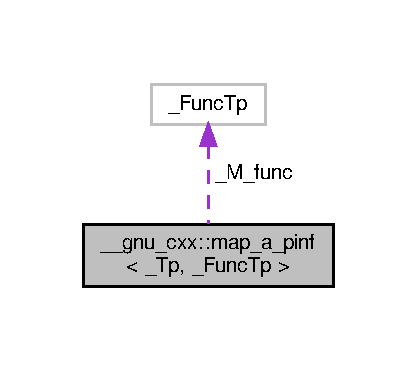
\includegraphics[width=200pt]{struct____gnu__cxx_1_1map__a__pinf__coll__graph}
\end{center}
\end{figure}
\subsection*{Public Member Functions}
\begin{DoxyCompactItemize}
\item 
\hyperlink{struct____gnu__cxx_1_1map__a__pinf_acc55db8d0a0fbe0bc604444dfecb2efe}{map\+\_\+a\+\_\+pinf} (\+\_\+\+Func\+Tp \hyperlink{namespace____gnu__cxx_af2b2f0c7a2ae72b922b1afefae5a65b2}{\+\_\+\+\_\+func}, \hyperlink{namespace____gnu__cxx_a3b19a9c800ca194374ef9172290f7d79}{\+\_\+\+Tp} \+\_\+\+\_\+a)
\item 
\hyperlink{namespace____gnu__cxx_a3b19a9c800ca194374ef9172290f7d79}{\+\_\+\+Tp} \hyperlink{struct____gnu__cxx_1_1map__a__pinf_afaf0f54109c7c496ce44603389bb495b}{operator()} (\hyperlink{namespace____gnu__cxx_a3b19a9c800ca194374ef9172290f7d79}{\+\_\+\+Tp} \+\_\+\+\_\+t) const
\end{DoxyCompactItemize}
\subsection*{Public Attributes}
\begin{DoxyCompactItemize}
\item 
const \hyperlink{namespace____gnu__cxx_a3b19a9c800ca194374ef9172290f7d79}{\+\_\+\+Tp} \hyperlink{struct____gnu__cxx_1_1map__a__pinf_a1de7ffe1b5ac3d528cb472ced4878f27}{\+\_\+\+M\+\_\+a}
\item 
\+\_\+\+Func\+Tp \hyperlink{struct____gnu__cxx_1_1map__a__pinf_a5e842585fa430caa329cb26a4976ee88}{\+\_\+\+M\+\_\+func}
\end{DoxyCompactItemize}


\subsection{Detailed Description}
\subsubsection*{template$<$typename \+\_\+\+Tp, typename \+\_\+\+Func\+Tp$>$\newline
struct \+\_\+\+\_\+gnu\+\_\+cxx\+::map\+\_\+a\+\_\+pinf$<$ \+\_\+\+Tp, \+\_\+\+Func\+Tp $>$}

Map a function defined on $ x \in [a, +\infty) $ to one defined on $ t \in (0, 1] $\+: \$f\mbox{[} \{a\}$^\wedge$\{+\}dx f(x) = \{0\}$^\wedge$\{1\}dt \{f(t)\}\{(1-\/t)$^\wedge$2\} \$f\mbox{]} \$f\mbox{[} x(t) = a + \{t\}\{1-\/t\} \$f\mbox{]} 

Definition at line 159 of file integration\+\_\+transform.\+h.



\subsection{Constructor \& Destructor Documentation}
\mbox{\Hypertarget{struct____gnu__cxx_1_1map__a__pinf_acc55db8d0a0fbe0bc604444dfecb2efe}\label{struct____gnu__cxx_1_1map__a__pinf_acc55db8d0a0fbe0bc604444dfecb2efe}} 
\index{\+\_\+\+\_\+gnu\+\_\+cxx\+::map\+\_\+a\+\_\+pinf@{\+\_\+\+\_\+gnu\+\_\+cxx\+::map\+\_\+a\+\_\+pinf}!map\+\_\+a\+\_\+pinf@{map\+\_\+a\+\_\+pinf}}
\index{map\+\_\+a\+\_\+pinf@{map\+\_\+a\+\_\+pinf}!\+\_\+\+\_\+gnu\+\_\+cxx\+::map\+\_\+a\+\_\+pinf@{\+\_\+\+\_\+gnu\+\_\+cxx\+::map\+\_\+a\+\_\+pinf}}
\subsubsection{\texorpdfstring{map\+\_\+a\+\_\+pinf()}{map\_a\_pinf()}}
{\footnotesize\ttfamily template$<$typename \+\_\+\+Tp , typename \+\_\+\+Func\+Tp $>$ \\
\hyperlink{struct____gnu__cxx_1_1map__a__pinf}{\+\_\+\+\_\+gnu\+\_\+cxx\+::map\+\_\+a\+\_\+pinf}$<$ \hyperlink{namespace____gnu__cxx_a3b19a9c800ca194374ef9172290f7d79}{\+\_\+\+Tp}, \+\_\+\+Func\+Tp $>$\+::\hyperlink{struct____gnu__cxx_1_1map__a__pinf}{map\+\_\+a\+\_\+pinf} (\begin{DoxyParamCaption}\item[{\+\_\+\+Func\+Tp}]{\+\_\+\+\_\+func,  }\item[{\hyperlink{namespace____gnu__cxx_a3b19a9c800ca194374ef9172290f7d79}{\+\_\+\+Tp}}]{\+\_\+\+\_\+a }\end{DoxyParamCaption})\hspace{0.3cm}{\ttfamily [inline]}}



Definition at line 164 of file integration\+\_\+transform.\+h.



References \+\_\+\+\_\+gnu\+\_\+cxx\+::\+\_\+\+Tp.


\begin{DoxyCode}
165       : \hyperlink{struct____gnu__cxx_1_1map__a__pinf_a5e842585fa430caa329cb26a4976ee88}{\_M\_func}(\hyperlink{namespace____gnu__cxx_af2b2f0c7a2ae72b922b1afefae5a65b2}{\_\_func}),
166         \hyperlink{struct____gnu__cxx_1_1map__a__pinf_a1de7ffe1b5ac3d528cb472ced4878f27}{\_M\_a}(\_\_a)
167       \{ \}
\end{DoxyCode}


\subsection{Member Function Documentation}
\mbox{\Hypertarget{struct____gnu__cxx_1_1map__a__pinf_afaf0f54109c7c496ce44603389bb495b}\label{struct____gnu__cxx_1_1map__a__pinf_afaf0f54109c7c496ce44603389bb495b}} 
\index{\+\_\+\+\_\+gnu\+\_\+cxx\+::map\+\_\+a\+\_\+pinf@{\+\_\+\+\_\+gnu\+\_\+cxx\+::map\+\_\+a\+\_\+pinf}!operator()@{operator()}}
\index{operator()@{operator()}!\+\_\+\+\_\+gnu\+\_\+cxx\+::map\+\_\+a\+\_\+pinf@{\+\_\+\+\_\+gnu\+\_\+cxx\+::map\+\_\+a\+\_\+pinf}}
\subsubsection{\texorpdfstring{operator()()}{operator()()}}
{\footnotesize\ttfamily template$<$typename \+\_\+\+Tp , typename \+\_\+\+Func\+Tp $>$ \\
\hyperlink{namespace____gnu__cxx_a3b19a9c800ca194374ef9172290f7d79}{\+\_\+\+Tp} \hyperlink{struct____gnu__cxx_1_1map__a__pinf}{\+\_\+\+\_\+gnu\+\_\+cxx\+::map\+\_\+a\+\_\+pinf}$<$ \hyperlink{namespace____gnu__cxx_a3b19a9c800ca194374ef9172290f7d79}{\+\_\+\+Tp}, \+\_\+\+Func\+Tp $>$\+::operator() (\begin{DoxyParamCaption}\item[{\hyperlink{namespace____gnu__cxx_a3b19a9c800ca194374ef9172290f7d79}{\+\_\+\+Tp}}]{\+\_\+\+\_\+t }\end{DoxyParamCaption}) const\hspace{0.3cm}{\ttfamily [inline]}}



Definition at line 170 of file integration\+\_\+transform.\+h.



References \+\_\+\+\_\+gnu\+\_\+cxx\+::mapper$<$ \+\_\+\+Tp, \+\_\+\+Func\+Tp $>$\+::\+\_\+\+M\+\_\+func, and \+\_\+\+\_\+gnu\+\_\+cxx\+::\+\_\+\+Tp.


\begin{DoxyCode}
171       \{
172         \textcolor{keywordflow}{if} (\_\_t == \hyperlink{namespace____gnu__cxx_a3b19a9c800ca194374ef9172290f7d79}{\_Tp}\{1\})
173           \textcolor{keywordflow}{return} \hyperlink{struct____gnu__cxx_1_1map__a__pinf_a5e842585fa430caa329cb26a4976ee88}{\_M\_func}(+std::numeric\_limits<\_Tp>::infinity());
174         \textcolor{keywordflow}{else}
175           \{
176             \textcolor{keyword}{const} \textcolor{keyword}{auto} \_\_inv\_1mt = \hyperlink{namespace____gnu__cxx_a3b19a9c800ca194374ef9172290f7d79}{\_Tp}\{1\} / (\hyperlink{namespace____gnu__cxx_a3b19a9c800ca194374ef9172290f7d79}{\_Tp}\{1\} - \_\_t);
177             \textcolor{keyword}{const} \textcolor{keyword}{auto} \_\_x = \hyperlink{struct____gnu__cxx_1_1map__a__pinf_a1de7ffe1b5ac3d528cb472ced4878f27}{\_M\_a} + \_\_t * \_\_inv\_1mt;
178             \textcolor{keyword}{const} \textcolor{keyword}{auto} \_\_y = \hyperlink{struct____gnu__cxx_1_1map__a__pinf_a5e842585fa430caa329cb26a4976ee88}{\_M\_func}(\_\_x);
179             \textcolor{keywordflow}{return} \_\_y * \_\_inv\_1mt * \_\_inv\_1mt;
180           \}
181       \}
\end{DoxyCode}


\subsection{Member Data Documentation}
\mbox{\Hypertarget{struct____gnu__cxx_1_1map__a__pinf_a1de7ffe1b5ac3d528cb472ced4878f27}\label{struct____gnu__cxx_1_1map__a__pinf_a1de7ffe1b5ac3d528cb472ced4878f27}} 
\index{\+\_\+\+\_\+gnu\+\_\+cxx\+::map\+\_\+a\+\_\+pinf@{\+\_\+\+\_\+gnu\+\_\+cxx\+::map\+\_\+a\+\_\+pinf}!\+\_\+\+M\+\_\+a@{\+\_\+\+M\+\_\+a}}
\index{\+\_\+\+M\+\_\+a@{\+\_\+\+M\+\_\+a}!\+\_\+\+\_\+gnu\+\_\+cxx\+::map\+\_\+a\+\_\+pinf@{\+\_\+\+\_\+gnu\+\_\+cxx\+::map\+\_\+a\+\_\+pinf}}
\subsubsection{\texorpdfstring{\+\_\+\+M\+\_\+a}{\_M\_a}}
{\footnotesize\ttfamily template$<$typename \+\_\+\+Tp , typename \+\_\+\+Func\+Tp $>$ \\
const \hyperlink{namespace____gnu__cxx_a3b19a9c800ca194374ef9172290f7d79}{\+\_\+\+Tp} \hyperlink{struct____gnu__cxx_1_1map__a__pinf}{\+\_\+\+\_\+gnu\+\_\+cxx\+::map\+\_\+a\+\_\+pinf}$<$ \hyperlink{namespace____gnu__cxx_a3b19a9c800ca194374ef9172290f7d79}{\+\_\+\+Tp}, \+\_\+\+Func\+Tp $>$\+::\+\_\+\+M\+\_\+a}



Definition at line 162 of file integration\+\_\+transform.\+h.

\mbox{\Hypertarget{struct____gnu__cxx_1_1map__a__pinf_a5e842585fa430caa329cb26a4976ee88}\label{struct____gnu__cxx_1_1map__a__pinf_a5e842585fa430caa329cb26a4976ee88}} 
\index{\+\_\+\+\_\+gnu\+\_\+cxx\+::map\+\_\+a\+\_\+pinf@{\+\_\+\+\_\+gnu\+\_\+cxx\+::map\+\_\+a\+\_\+pinf}!\+\_\+\+M\+\_\+func@{\+\_\+\+M\+\_\+func}}
\index{\+\_\+\+M\+\_\+func@{\+\_\+\+M\+\_\+func}!\+\_\+\+\_\+gnu\+\_\+cxx\+::map\+\_\+a\+\_\+pinf@{\+\_\+\+\_\+gnu\+\_\+cxx\+::map\+\_\+a\+\_\+pinf}}
\subsubsection{\texorpdfstring{\+\_\+\+M\+\_\+func}{\_M\_func}}
{\footnotesize\ttfamily template$<$typename \+\_\+\+Tp , typename \+\_\+\+Func\+Tp $>$ \\
\+\_\+\+Func\+Tp \hyperlink{struct____gnu__cxx_1_1map__a__pinf}{\+\_\+\+\_\+gnu\+\_\+cxx\+::map\+\_\+a\+\_\+pinf}$<$ \hyperlink{namespace____gnu__cxx_a3b19a9c800ca194374ef9172290f7d79}{\+\_\+\+Tp}, \+\_\+\+Func\+Tp $>$\+::\+\_\+\+M\+\_\+func}



Definition at line 161 of file integration\+\_\+transform.\+h.



The documentation for this struct was generated from the following file\+:\begin{DoxyCompactItemize}
\item 
include/ext/\hyperlink{integration__transform_8h}{integration\+\_\+transform.\+h}\end{DoxyCompactItemize}

\hypertarget{struct____gnu__cxx_1_1map__minf__b}{}\section{\+\_\+\+\_\+gnu\+\_\+cxx\+:\+:map\+\_\+minf\+\_\+b$<$ \+\_\+\+Tp, \+\_\+\+Func\+Tp $>$ Struct Template Reference}
\label{struct____gnu__cxx_1_1map__minf__b}\index{\+\_\+\+\_\+gnu\+\_\+cxx\+::map\+\_\+minf\+\_\+b$<$ \+\_\+\+Tp, \+\_\+\+Func\+Tp $>$@{\+\_\+\+\_\+gnu\+\_\+cxx\+::map\+\_\+minf\+\_\+b$<$ \+\_\+\+Tp, \+\_\+\+Func\+Tp $>$}}


{\ttfamily \#include $<$integration\+\_\+transform.\+h$>$}



Collaboration diagram for \+\_\+\+\_\+gnu\+\_\+cxx\+:\+:map\+\_\+minf\+\_\+b$<$ \+\_\+\+Tp, \+\_\+\+Func\+Tp $>$\+:
\nopagebreak
\begin{figure}[H]
\begin{center}
\leavevmode
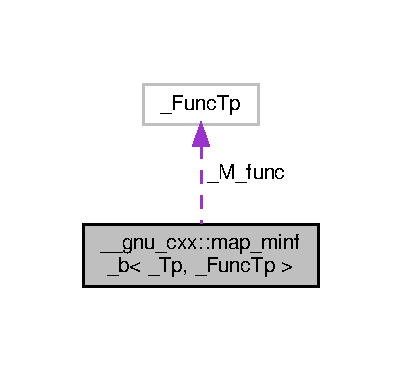
\includegraphics[width=193pt]{struct____gnu__cxx_1_1map__minf__b__coll__graph}
\end{center}
\end{figure}
\subsection*{Public Member Functions}
\begin{DoxyCompactItemize}
\item 
\hyperlink{struct____gnu__cxx_1_1map__minf__b_a55f2ab1a754dcf6068232d8186a194da}{map\+\_\+minf\+\_\+b} (\+\_\+\+Func\+Tp \hyperlink{namespace____gnu__cxx_af2b2f0c7a2ae72b922b1afefae5a65b2}{\+\_\+\+\_\+func}, \hyperlink{namespace____gnu__cxx_a3b19a9c800ca194374ef9172290f7d79}{\+\_\+\+Tp} \+\_\+\+\_\+b)
\item 
\hyperlink{namespace____gnu__cxx_a3b19a9c800ca194374ef9172290f7d79}{\+\_\+\+Tp} \hyperlink{struct____gnu__cxx_1_1map__minf__b_a4e9a67a4d37675e4c1ca3e0bff74ade3}{operator()} (\hyperlink{namespace____gnu__cxx_a3b19a9c800ca194374ef9172290f7d79}{\+\_\+\+Tp} \+\_\+\+\_\+t) const
\end{DoxyCompactItemize}
\subsection*{Public Attributes}
\begin{DoxyCompactItemize}
\item 
const \hyperlink{namespace____gnu__cxx_a3b19a9c800ca194374ef9172290f7d79}{\+\_\+\+Tp} \hyperlink{struct____gnu__cxx_1_1map__minf__b_a03b2c7b30f21200812f87251cd0aff66}{\+\_\+\+M\+\_\+b}
\item 
\+\_\+\+Func\+Tp \hyperlink{struct____gnu__cxx_1_1map__minf__b_a6eeb7b723b6bb691690adfbdec7b4648}{\+\_\+\+M\+\_\+func}
\end{DoxyCompactItemize}


\subsection{Detailed Description}
\subsubsection*{template$<$typename \+\_\+\+Tp, typename \+\_\+\+Func\+Tp$>$\newline
struct \+\_\+\+\_\+gnu\+\_\+cxx\+::map\+\_\+minf\+\_\+b$<$ \+\_\+\+Tp, \+\_\+\+Func\+Tp $>$}

Map a function defined on $ x \in (-\infty, b] $ to one defined on $ t \in (0, 1] $\+: \$f\mbox{[} \{-\/\}$^\wedge$\{b\}dx f(x) = \{0\}$^\wedge$\{1\}dt \{f(t)\}\{t$^\wedge$2\} \$f\mbox{]} \$f\mbox{[} x(t) = b -\/ \{1-\/t\}\{t\} \$f\mbox{]} 

Definition at line 123 of file integration\+\_\+transform.\+h.



\subsection{Constructor \& Destructor Documentation}
\mbox{\Hypertarget{struct____gnu__cxx_1_1map__minf__b_a55f2ab1a754dcf6068232d8186a194da}\label{struct____gnu__cxx_1_1map__minf__b_a55f2ab1a754dcf6068232d8186a194da}} 
\index{\+\_\+\+\_\+gnu\+\_\+cxx\+::map\+\_\+minf\+\_\+b@{\+\_\+\+\_\+gnu\+\_\+cxx\+::map\+\_\+minf\+\_\+b}!map\+\_\+minf\+\_\+b@{map\+\_\+minf\+\_\+b}}
\index{map\+\_\+minf\+\_\+b@{map\+\_\+minf\+\_\+b}!\+\_\+\+\_\+gnu\+\_\+cxx\+::map\+\_\+minf\+\_\+b@{\+\_\+\+\_\+gnu\+\_\+cxx\+::map\+\_\+minf\+\_\+b}}
\subsubsection{\texorpdfstring{map\+\_\+minf\+\_\+b()}{map\_minf\_b()}}
{\footnotesize\ttfamily template$<$typename \+\_\+\+Tp , typename \+\_\+\+Func\+Tp $>$ \\
\hyperlink{struct____gnu__cxx_1_1map__minf__b}{\+\_\+\+\_\+gnu\+\_\+cxx\+::map\+\_\+minf\+\_\+b}$<$ \hyperlink{namespace____gnu__cxx_a3b19a9c800ca194374ef9172290f7d79}{\+\_\+\+Tp}, \+\_\+\+Func\+Tp $>$\+::\hyperlink{struct____gnu__cxx_1_1map__minf__b}{map\+\_\+minf\+\_\+b} (\begin{DoxyParamCaption}\item[{\+\_\+\+Func\+Tp}]{\+\_\+\+\_\+func,  }\item[{\hyperlink{namespace____gnu__cxx_a3b19a9c800ca194374ef9172290f7d79}{\+\_\+\+Tp}}]{\+\_\+\+\_\+b }\end{DoxyParamCaption})\hspace{0.3cm}{\ttfamily [inline]}}



Definition at line 128 of file integration\+\_\+transform.\+h.



References \+\_\+\+\_\+gnu\+\_\+cxx\+::\+\_\+\+Tp.


\begin{DoxyCode}
129       : \hyperlink{struct____gnu__cxx_1_1map__minf__b_a6eeb7b723b6bb691690adfbdec7b4648}{\_M\_func}(\hyperlink{namespace____gnu__cxx_af2b2f0c7a2ae72b922b1afefae5a65b2}{\_\_func}),
130         \hyperlink{struct____gnu__cxx_1_1map__minf__b_a03b2c7b30f21200812f87251cd0aff66}{\_M\_b}(\_\_b)
131       \{ \}
\end{DoxyCode}


\subsection{Member Function Documentation}
\mbox{\Hypertarget{struct____gnu__cxx_1_1map__minf__b_a4e9a67a4d37675e4c1ca3e0bff74ade3}\label{struct____gnu__cxx_1_1map__minf__b_a4e9a67a4d37675e4c1ca3e0bff74ade3}} 
\index{\+\_\+\+\_\+gnu\+\_\+cxx\+::map\+\_\+minf\+\_\+b@{\+\_\+\+\_\+gnu\+\_\+cxx\+::map\+\_\+minf\+\_\+b}!operator()@{operator()}}
\index{operator()@{operator()}!\+\_\+\+\_\+gnu\+\_\+cxx\+::map\+\_\+minf\+\_\+b@{\+\_\+\+\_\+gnu\+\_\+cxx\+::map\+\_\+minf\+\_\+b}}
\subsubsection{\texorpdfstring{operator()()}{operator()()}}
{\footnotesize\ttfamily template$<$typename \+\_\+\+Tp , typename \+\_\+\+Func\+Tp $>$ \\
\hyperlink{namespace____gnu__cxx_a3b19a9c800ca194374ef9172290f7d79}{\+\_\+\+Tp} \hyperlink{struct____gnu__cxx_1_1map__minf__b}{\+\_\+\+\_\+gnu\+\_\+cxx\+::map\+\_\+minf\+\_\+b}$<$ \hyperlink{namespace____gnu__cxx_a3b19a9c800ca194374ef9172290f7d79}{\+\_\+\+Tp}, \+\_\+\+Func\+Tp $>$\+::operator() (\begin{DoxyParamCaption}\item[{\hyperlink{namespace____gnu__cxx_a3b19a9c800ca194374ef9172290f7d79}{\+\_\+\+Tp}}]{\+\_\+\+\_\+t }\end{DoxyParamCaption}) const\hspace{0.3cm}{\ttfamily [inline]}}



Definition at line 134 of file integration\+\_\+transform.\+h.



References \+\_\+\+\_\+gnu\+\_\+cxx\+::mapper$<$ \+\_\+\+Tp, \+\_\+\+Func\+Tp $>$\+::\+\_\+\+M\+\_\+func, and \+\_\+\+\_\+gnu\+\_\+cxx\+::\+\_\+\+Tp.


\begin{DoxyCode}
135       \{
136         \textcolor{keywordflow}{if} (\_\_t == \hyperlink{namespace____gnu__cxx_a3b19a9c800ca194374ef9172290f7d79}{\_Tp}\{0\})
137           \textcolor{keywordflow}{return} \hyperlink{struct____gnu__cxx_1_1map__minf__b_a6eeb7b723b6bb691690adfbdec7b4648}{\_M\_func}(-std::numeric\_limits<\_Tp>::infinity());
138         \textcolor{keywordflow}{else}
139           \{
140             \textcolor{keyword}{const} \textcolor{keyword}{auto} \_\_inv\_t = \hyperlink{namespace____gnu__cxx_a3b19a9c800ca194374ef9172290f7d79}{\_Tp}\{1\} / \_\_t;
141             \textcolor{keyword}{const} \textcolor{keyword}{auto} \_\_x = \hyperlink{struct____gnu__cxx_1_1map__minf__b_a03b2c7b30f21200812f87251cd0aff66}{\_M\_b} - (\hyperlink{namespace____gnu__cxx_a3b19a9c800ca194374ef9172290f7d79}{\_Tp}\{1\} - \_\_t) * \_\_inv\_t;
142             \textcolor{keyword}{const} \textcolor{keyword}{auto} \_\_y = \hyperlink{struct____gnu__cxx_1_1map__minf__b_a6eeb7b723b6bb691690adfbdec7b4648}{\_M\_func}(\_\_x);
143             \textcolor{keywordflow}{return} \_\_y * \_\_inv\_t * \_\_inv\_t;
144           \}
145       \}
\end{DoxyCode}


\subsection{Member Data Documentation}
\mbox{\Hypertarget{struct____gnu__cxx_1_1map__minf__b_a03b2c7b30f21200812f87251cd0aff66}\label{struct____gnu__cxx_1_1map__minf__b_a03b2c7b30f21200812f87251cd0aff66}} 
\index{\+\_\+\+\_\+gnu\+\_\+cxx\+::map\+\_\+minf\+\_\+b@{\+\_\+\+\_\+gnu\+\_\+cxx\+::map\+\_\+minf\+\_\+b}!\+\_\+\+M\+\_\+b@{\+\_\+\+M\+\_\+b}}
\index{\+\_\+\+M\+\_\+b@{\+\_\+\+M\+\_\+b}!\+\_\+\+\_\+gnu\+\_\+cxx\+::map\+\_\+minf\+\_\+b@{\+\_\+\+\_\+gnu\+\_\+cxx\+::map\+\_\+minf\+\_\+b}}
\subsubsection{\texorpdfstring{\+\_\+\+M\+\_\+b}{\_M\_b}}
{\footnotesize\ttfamily template$<$typename \+\_\+\+Tp , typename \+\_\+\+Func\+Tp $>$ \\
const \hyperlink{namespace____gnu__cxx_a3b19a9c800ca194374ef9172290f7d79}{\+\_\+\+Tp} \hyperlink{struct____gnu__cxx_1_1map__minf__b}{\+\_\+\+\_\+gnu\+\_\+cxx\+::map\+\_\+minf\+\_\+b}$<$ \hyperlink{namespace____gnu__cxx_a3b19a9c800ca194374ef9172290f7d79}{\+\_\+\+Tp}, \+\_\+\+Func\+Tp $>$\+::\+\_\+\+M\+\_\+b}



Definition at line 126 of file integration\+\_\+transform.\+h.

\mbox{\Hypertarget{struct____gnu__cxx_1_1map__minf__b_a6eeb7b723b6bb691690adfbdec7b4648}\label{struct____gnu__cxx_1_1map__minf__b_a6eeb7b723b6bb691690adfbdec7b4648}} 
\index{\+\_\+\+\_\+gnu\+\_\+cxx\+::map\+\_\+minf\+\_\+b@{\+\_\+\+\_\+gnu\+\_\+cxx\+::map\+\_\+minf\+\_\+b}!\+\_\+\+M\+\_\+func@{\+\_\+\+M\+\_\+func}}
\index{\+\_\+\+M\+\_\+func@{\+\_\+\+M\+\_\+func}!\+\_\+\+\_\+gnu\+\_\+cxx\+::map\+\_\+minf\+\_\+b@{\+\_\+\+\_\+gnu\+\_\+cxx\+::map\+\_\+minf\+\_\+b}}
\subsubsection{\texorpdfstring{\+\_\+\+M\+\_\+func}{\_M\_func}}
{\footnotesize\ttfamily template$<$typename \+\_\+\+Tp , typename \+\_\+\+Func\+Tp $>$ \\
\+\_\+\+Func\+Tp \hyperlink{struct____gnu__cxx_1_1map__minf__b}{\+\_\+\+\_\+gnu\+\_\+cxx\+::map\+\_\+minf\+\_\+b}$<$ \hyperlink{namespace____gnu__cxx_a3b19a9c800ca194374ef9172290f7d79}{\+\_\+\+Tp}, \+\_\+\+Func\+Tp $>$\+::\+\_\+\+M\+\_\+func}



Definition at line 125 of file integration\+\_\+transform.\+h.



The documentation for this struct was generated from the following file\+:\begin{DoxyCompactItemize}
\item 
include/ext/\hyperlink{integration__transform_8h}{integration\+\_\+transform.\+h}\end{DoxyCompactItemize}

\hypertarget{struct____gnu__cxx_1_1map__minf__pinf}{}\section{\+\_\+\+\_\+gnu\+\_\+cxx\+:\+:map\+\_\+minf\+\_\+pinf$<$ \+\_\+\+Tp, \+\_\+\+Func\+Tp $>$ Struct Template Reference}
\label{struct____gnu__cxx_1_1map__minf__pinf}\index{\+\_\+\+\_\+gnu\+\_\+cxx\+::map\+\_\+minf\+\_\+pinf$<$ \+\_\+\+Tp, \+\_\+\+Func\+Tp $>$@{\+\_\+\+\_\+gnu\+\_\+cxx\+::map\+\_\+minf\+\_\+pinf$<$ \+\_\+\+Tp, \+\_\+\+Func\+Tp $>$}}


{\ttfamily \#include $<$integration\+\_\+transform.\+h$>$}



Collaboration diagram for \+\_\+\+\_\+gnu\+\_\+cxx\+:\+:map\+\_\+minf\+\_\+pinf$<$ \+\_\+\+Tp, \+\_\+\+Func\+Tp $>$\+:
\nopagebreak
\begin{figure}[H]
\begin{center}
\leavevmode
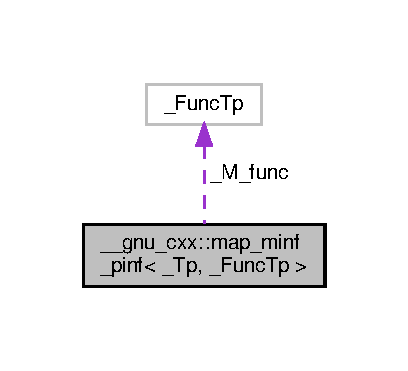
\includegraphics[width=196pt]{struct____gnu__cxx_1_1map__minf__pinf__coll__graph}
\end{center}
\end{figure}
\subsection*{Public Member Functions}
\begin{DoxyCompactItemize}
\item 
\hyperlink{struct____gnu__cxx_1_1map__minf__pinf_a7ffd9d3da4cb973ffe3f2fc6423f5491}{map\+\_\+minf\+\_\+pinf} (\+\_\+\+Func\+Tp \hyperlink{namespace____gnu__cxx_af2b2f0c7a2ae72b922b1afefae5a65b2}{\+\_\+\+\_\+func})
\item 
\hyperlink{namespace____gnu__cxx_a3b19a9c800ca194374ef9172290f7d79}{\+\_\+\+Tp} \hyperlink{struct____gnu__cxx_1_1map__minf__pinf_a39669672f547fb7979406452ec84bbc7}{operator()} (\hyperlink{namespace____gnu__cxx_a3b19a9c800ca194374ef9172290f7d79}{\+\_\+\+Tp} \+\_\+\+\_\+t) const
\end{DoxyCompactItemize}
\subsection*{Public Attributes}
\begin{DoxyCompactItemize}
\item 
\+\_\+\+Func\+Tp \hyperlink{struct____gnu__cxx_1_1map__minf__pinf_a38f287d24e3b40dc964637ac5e8f2532}{\+\_\+\+M\+\_\+func}
\end{DoxyCompactItemize}


\subsection{Detailed Description}
\subsubsection*{template$<$typename \+\_\+\+Tp, typename \+\_\+\+Func\+Tp$>$\newline
struct \+\_\+\+\_\+gnu\+\_\+cxx\+::map\+\_\+minf\+\_\+pinf$<$ \+\_\+\+Tp, \+\_\+\+Func\+Tp $>$}

Map a function defined on $ x \in (-\infty, +\infty) $ to one defined on $ t \in (0, 1) $\+: \$f\mbox{[} \{-\/\}$^\wedge$\{+\}dx f(x) = \{0\}$^\wedge$\{1\}dt \{f(t)\}\{t$^\wedge$2\} \$f\mbox{]} \$f\mbox{[} x(t) = -\/\{1\}\{t\} + \{1\}\{1-\/t\} \$f\mbox{]} 

Definition at line 86 of file integration\+\_\+transform.\+h.



\subsection{Constructor \& Destructor Documentation}
\mbox{\Hypertarget{struct____gnu__cxx_1_1map__minf__pinf_a7ffd9d3da4cb973ffe3f2fc6423f5491}\label{struct____gnu__cxx_1_1map__minf__pinf_a7ffd9d3da4cb973ffe3f2fc6423f5491}} 
\index{\+\_\+\+\_\+gnu\+\_\+cxx\+::map\+\_\+minf\+\_\+pinf@{\+\_\+\+\_\+gnu\+\_\+cxx\+::map\+\_\+minf\+\_\+pinf}!map\+\_\+minf\+\_\+pinf@{map\+\_\+minf\+\_\+pinf}}
\index{map\+\_\+minf\+\_\+pinf@{map\+\_\+minf\+\_\+pinf}!\+\_\+\+\_\+gnu\+\_\+cxx\+::map\+\_\+minf\+\_\+pinf@{\+\_\+\+\_\+gnu\+\_\+cxx\+::map\+\_\+minf\+\_\+pinf}}
\subsubsection{\texorpdfstring{map\+\_\+minf\+\_\+pinf()}{map\_minf\_pinf()}}
{\footnotesize\ttfamily template$<$typename \+\_\+\+Tp , typename \+\_\+\+Func\+Tp $>$ \\
\hyperlink{struct____gnu__cxx_1_1map__minf__pinf}{\+\_\+\+\_\+gnu\+\_\+cxx\+::map\+\_\+minf\+\_\+pinf}$<$ \hyperlink{namespace____gnu__cxx_a3b19a9c800ca194374ef9172290f7d79}{\+\_\+\+Tp}, \+\_\+\+Func\+Tp $>$\+::\hyperlink{struct____gnu__cxx_1_1map__minf__pinf}{map\+\_\+minf\+\_\+pinf} (\begin{DoxyParamCaption}\item[{\+\_\+\+Func\+Tp}]{\+\_\+\+\_\+func }\end{DoxyParamCaption})\hspace{0.3cm}{\ttfamily [inline]}}



Definition at line 90 of file integration\+\_\+transform.\+h.



References \+\_\+\+\_\+gnu\+\_\+cxx\+::\+\_\+\+Tp.


\begin{DoxyCode}
91       : \hyperlink{struct____gnu__cxx_1_1map__minf__pinf_a38f287d24e3b40dc964637ac5e8f2532}{\_M\_func}(\hyperlink{namespace____gnu__cxx_af2b2f0c7a2ae72b922b1afefae5a65b2}{\_\_func})
92       \{ \}
\end{DoxyCode}


\subsection{Member Function Documentation}
\mbox{\Hypertarget{struct____gnu__cxx_1_1map__minf__pinf_a39669672f547fb7979406452ec84bbc7}\label{struct____gnu__cxx_1_1map__minf__pinf_a39669672f547fb7979406452ec84bbc7}} 
\index{\+\_\+\+\_\+gnu\+\_\+cxx\+::map\+\_\+minf\+\_\+pinf@{\+\_\+\+\_\+gnu\+\_\+cxx\+::map\+\_\+minf\+\_\+pinf}!operator()@{operator()}}
\index{operator()@{operator()}!\+\_\+\+\_\+gnu\+\_\+cxx\+::map\+\_\+minf\+\_\+pinf@{\+\_\+\+\_\+gnu\+\_\+cxx\+::map\+\_\+minf\+\_\+pinf}}
\subsubsection{\texorpdfstring{operator()()}{operator()()}}
{\footnotesize\ttfamily template$<$typename \+\_\+\+Tp , typename \+\_\+\+Func\+Tp $>$ \\
\hyperlink{namespace____gnu__cxx_a3b19a9c800ca194374ef9172290f7d79}{\+\_\+\+Tp} \hyperlink{struct____gnu__cxx_1_1map__minf__pinf}{\+\_\+\+\_\+gnu\+\_\+cxx\+::map\+\_\+minf\+\_\+pinf}$<$ \hyperlink{namespace____gnu__cxx_a3b19a9c800ca194374ef9172290f7d79}{\+\_\+\+Tp}, \+\_\+\+Func\+Tp $>$\+::operator() (\begin{DoxyParamCaption}\item[{\hyperlink{namespace____gnu__cxx_a3b19a9c800ca194374ef9172290f7d79}{\+\_\+\+Tp}}]{\+\_\+\+\_\+t }\end{DoxyParamCaption}) const\hspace{0.3cm}{\ttfamily [inline]}}



Definition at line 95 of file integration\+\_\+transform.\+h.



References \+\_\+\+\_\+gnu\+\_\+cxx\+::mapper$<$ \+\_\+\+Tp, \+\_\+\+Func\+Tp $>$\+::\+\_\+\+M\+\_\+func, and \+\_\+\+\_\+gnu\+\_\+cxx\+::\+\_\+\+Tp.


\begin{DoxyCode}
96       \{
97         \textcolor{keywordflow}{if} (\_\_t == \hyperlink{namespace____gnu__cxx_a3b19a9c800ca194374ef9172290f7d79}{\_Tp}\{0\})
98           \textcolor{keywordflow}{return} \hyperlink{struct____gnu__cxx_1_1map__minf__pinf_a38f287d24e3b40dc964637ac5e8f2532}{\_M\_func}(-std::numeric\_limits<\_Tp>::infinity());
99         \textcolor{keywordflow}{else} \textcolor{keywordflow}{if} (\_\_t == \hyperlink{namespace____gnu__cxx_a3b19a9c800ca194374ef9172290f7d79}{\_Tp}\{1\})
100           \textcolor{keywordflow}{return} \hyperlink{struct____gnu__cxx_1_1map__minf__pinf_a38f287d24e3b40dc964637ac5e8f2532}{\_M\_func}(+std::numeric\_limits<\_Tp>::infinity());
101         \textcolor{keywordflow}{else}
102           \{
103             \textcolor{keyword}{const} \textcolor{keyword}{auto} \_\_inv\_t = \hyperlink{namespace____gnu__cxx_a3b19a9c800ca194374ef9172290f7d79}{\_Tp}\{1\} / \_\_t;
104             \textcolor{keyword}{const} \textcolor{keyword}{auto} \_\_inv\_1mt = \hyperlink{namespace____gnu__cxx_a3b19a9c800ca194374ef9172290f7d79}{\_Tp}\{1\} / (\hyperlink{namespace____gnu__cxx_a3b19a9c800ca194374ef9172290f7d79}{\_Tp}\{1\} - \_\_t);
105             \textcolor{keyword}{const} \textcolor{keyword}{auto} \_\_x = -\_\_inv\_t + \_\_inv\_1mt;
106             \textcolor{keyword}{const} \textcolor{keyword}{auto} \_\_y = \hyperlink{struct____gnu__cxx_1_1map__minf__pinf_a38f287d24e3b40dc964637ac5e8f2532}{\_M\_func}(\_\_x);
107             \textcolor{keywordflow}{return} \_\_y * (\_\_inv\_t * \_\_inv\_t + \_\_inv\_1mt * \_\_inv\_1mt);
108           \}
109       \}
\end{DoxyCode}


\subsection{Member Data Documentation}
\mbox{\Hypertarget{struct____gnu__cxx_1_1map__minf__pinf_a38f287d24e3b40dc964637ac5e8f2532}\label{struct____gnu__cxx_1_1map__minf__pinf_a38f287d24e3b40dc964637ac5e8f2532}} 
\index{\+\_\+\+\_\+gnu\+\_\+cxx\+::map\+\_\+minf\+\_\+pinf@{\+\_\+\+\_\+gnu\+\_\+cxx\+::map\+\_\+minf\+\_\+pinf}!\+\_\+\+M\+\_\+func@{\+\_\+\+M\+\_\+func}}
\index{\+\_\+\+M\+\_\+func@{\+\_\+\+M\+\_\+func}!\+\_\+\+\_\+gnu\+\_\+cxx\+::map\+\_\+minf\+\_\+pinf@{\+\_\+\+\_\+gnu\+\_\+cxx\+::map\+\_\+minf\+\_\+pinf}}
\subsubsection{\texorpdfstring{\+\_\+\+M\+\_\+func}{\_M\_func}}
{\footnotesize\ttfamily template$<$typename \+\_\+\+Tp , typename \+\_\+\+Func\+Tp $>$ \\
\+\_\+\+Func\+Tp \hyperlink{struct____gnu__cxx_1_1map__minf__pinf}{\+\_\+\+\_\+gnu\+\_\+cxx\+::map\+\_\+minf\+\_\+pinf}$<$ \hyperlink{namespace____gnu__cxx_a3b19a9c800ca194374ef9172290f7d79}{\+\_\+\+Tp}, \+\_\+\+Func\+Tp $>$\+::\+\_\+\+M\+\_\+func}



Definition at line 88 of file integration\+\_\+transform.\+h.



The documentation for this struct was generated from the following file\+:\begin{DoxyCompactItemize}
\item 
include/ext/\hyperlink{integration__transform_8h}{integration\+\_\+transform.\+h}\end{DoxyCompactItemize}

\hypertarget{struct____gnu__cxx_1_1map__minf__pinf__symm}{}\section{\+\_\+\+\_\+gnu\+\_\+cxx\+:\+:map\+\_\+minf\+\_\+pinf\+\_\+symm$<$ \+\_\+\+Tp, \+\_\+\+Func\+Tp $>$ Struct Template Reference}
\label{struct____gnu__cxx_1_1map__minf__pinf__symm}\index{\+\_\+\+\_\+gnu\+\_\+cxx\+::map\+\_\+minf\+\_\+pinf\+\_\+symm$<$ \+\_\+\+Tp, \+\_\+\+Func\+Tp $>$@{\+\_\+\+\_\+gnu\+\_\+cxx\+::map\+\_\+minf\+\_\+pinf\+\_\+symm$<$ \+\_\+\+Tp, \+\_\+\+Func\+Tp $>$}}


{\ttfamily \#include $<$integration\+\_\+transform.\+h$>$}



Collaboration diagram for \+\_\+\+\_\+gnu\+\_\+cxx\+:\+:map\+\_\+minf\+\_\+pinf\+\_\+symm$<$ \+\_\+\+Tp, \+\_\+\+Func\+Tp $>$\+:
\nopagebreak
\begin{figure}[H]
\begin{center}
\leavevmode
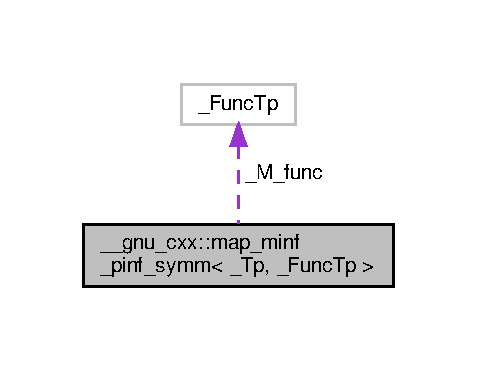
\includegraphics[width=229pt]{struct____gnu__cxx_1_1map__minf__pinf__symm__coll__graph}
\end{center}
\end{figure}
\subsection*{Public Member Functions}
\begin{DoxyCompactItemize}
\item 
\hyperlink{struct____gnu__cxx_1_1map__minf__pinf__symm_a31f5258be5cf1e1e9fc7b2157fe73461}{map\+\_\+minf\+\_\+pinf\+\_\+symm} (\+\_\+\+Func\+Tp \hyperlink{namespace____gnu__cxx_af2b2f0c7a2ae72b922b1afefae5a65b2}{\+\_\+\+\_\+func})
\item 
\hyperlink{namespace____gnu__cxx_a3b19a9c800ca194374ef9172290f7d79}{\+\_\+\+Tp} \hyperlink{struct____gnu__cxx_1_1map__minf__pinf__symm_a9814773879a6ccd8379237161697dfe8}{operator()} (\hyperlink{namespace____gnu__cxx_a3b19a9c800ca194374ef9172290f7d79}{\+\_\+\+Tp} \+\_\+\+\_\+t) const
\end{DoxyCompactItemize}
\subsection*{Public Attributes}
\begin{DoxyCompactItemize}
\item 
\+\_\+\+Func\+Tp \hyperlink{struct____gnu__cxx_1_1map__minf__pinf__symm_a3e6d1d72fb8471f11573dc8b6ce835c6}{\+\_\+\+M\+\_\+func}
\end{DoxyCompactItemize}


\subsection{Detailed Description}
\subsubsection*{template$<$typename \+\_\+\+Tp, typename \+\_\+\+Func\+Tp$>$\newline
struct \+\_\+\+\_\+gnu\+\_\+cxx\+::map\+\_\+minf\+\_\+pinf\+\_\+symm$<$ \+\_\+\+Tp, \+\_\+\+Func\+Tp $>$}

Map a function defined on $ x \in (-\infty, +\infty) $ to one defined on $ t \in (0, 1] $\+: \$f\mbox{[} \{-\/\}$^\wedge$\{+\}dx f(x) = \{0\}$^\wedge$\{1\}dt \{f(t)\}\{t$^\wedge$2\} \$f\mbox{]} \$f\mbox{[} x(t) = \{1-\/t\}\{t\} \$f\mbox{]} Note\+: $ g(t) $ actually returns $ [f(-x) + f(+x)]dx/dt $. Note\+: $ x:0->\infty $ as $ t:1->0 $. 

Definition at line 51 of file integration\+\_\+transform.\+h.



\subsection{Constructor \& Destructor Documentation}
\mbox{\Hypertarget{struct____gnu__cxx_1_1map__minf__pinf__symm_a31f5258be5cf1e1e9fc7b2157fe73461}\label{struct____gnu__cxx_1_1map__minf__pinf__symm_a31f5258be5cf1e1e9fc7b2157fe73461}} 
\index{\+\_\+\+\_\+gnu\+\_\+cxx\+::map\+\_\+minf\+\_\+pinf\+\_\+symm@{\+\_\+\+\_\+gnu\+\_\+cxx\+::map\+\_\+minf\+\_\+pinf\+\_\+symm}!map\+\_\+minf\+\_\+pinf\+\_\+symm@{map\+\_\+minf\+\_\+pinf\+\_\+symm}}
\index{map\+\_\+minf\+\_\+pinf\+\_\+symm@{map\+\_\+minf\+\_\+pinf\+\_\+symm}!\+\_\+\+\_\+gnu\+\_\+cxx\+::map\+\_\+minf\+\_\+pinf\+\_\+symm@{\+\_\+\+\_\+gnu\+\_\+cxx\+::map\+\_\+minf\+\_\+pinf\+\_\+symm}}
\subsubsection{\texorpdfstring{map\+\_\+minf\+\_\+pinf\+\_\+symm()}{map\_minf\_pinf\_symm()}}
{\footnotesize\ttfamily template$<$typename \+\_\+\+Tp , typename \+\_\+\+Func\+Tp $>$ \\
\hyperlink{struct____gnu__cxx_1_1map__minf__pinf__symm}{\+\_\+\+\_\+gnu\+\_\+cxx\+::map\+\_\+minf\+\_\+pinf\+\_\+symm}$<$ \hyperlink{namespace____gnu__cxx_a3b19a9c800ca194374ef9172290f7d79}{\+\_\+\+Tp}, \+\_\+\+Func\+Tp $>$\+::\hyperlink{struct____gnu__cxx_1_1map__minf__pinf__symm}{map\+\_\+minf\+\_\+pinf\+\_\+symm} (\begin{DoxyParamCaption}\item[{\+\_\+\+Func\+Tp}]{\+\_\+\+\_\+func }\end{DoxyParamCaption})\hspace{0.3cm}{\ttfamily [inline]}}



Definition at line 55 of file integration\+\_\+transform.\+h.



References \+\_\+\+\_\+gnu\+\_\+cxx\+::\+\_\+\+Tp.


\begin{DoxyCode}
56       : \hyperlink{struct____gnu__cxx_1_1map__minf__pinf__symm_a3e6d1d72fb8471f11573dc8b6ce835c6}{\_M\_func}(\hyperlink{namespace____gnu__cxx_af2b2f0c7a2ae72b922b1afefae5a65b2}{\_\_func})
57       \{ \}
\end{DoxyCode}


\subsection{Member Function Documentation}
\mbox{\Hypertarget{struct____gnu__cxx_1_1map__minf__pinf__symm_a9814773879a6ccd8379237161697dfe8}\label{struct____gnu__cxx_1_1map__minf__pinf__symm_a9814773879a6ccd8379237161697dfe8}} 
\index{\+\_\+\+\_\+gnu\+\_\+cxx\+::map\+\_\+minf\+\_\+pinf\+\_\+symm@{\+\_\+\+\_\+gnu\+\_\+cxx\+::map\+\_\+minf\+\_\+pinf\+\_\+symm}!operator()@{operator()}}
\index{operator()@{operator()}!\+\_\+\+\_\+gnu\+\_\+cxx\+::map\+\_\+minf\+\_\+pinf\+\_\+symm@{\+\_\+\+\_\+gnu\+\_\+cxx\+::map\+\_\+minf\+\_\+pinf\+\_\+symm}}
\subsubsection{\texorpdfstring{operator()()}{operator()()}}
{\footnotesize\ttfamily template$<$typename \+\_\+\+Tp , typename \+\_\+\+Func\+Tp $>$ \\
\hyperlink{namespace____gnu__cxx_a3b19a9c800ca194374ef9172290f7d79}{\+\_\+\+Tp} \hyperlink{struct____gnu__cxx_1_1map__minf__pinf__symm}{\+\_\+\+\_\+gnu\+\_\+cxx\+::map\+\_\+minf\+\_\+pinf\+\_\+symm}$<$ \hyperlink{namespace____gnu__cxx_a3b19a9c800ca194374ef9172290f7d79}{\+\_\+\+Tp}, \+\_\+\+Func\+Tp $>$\+::operator() (\begin{DoxyParamCaption}\item[{\hyperlink{namespace____gnu__cxx_a3b19a9c800ca194374ef9172290f7d79}{\+\_\+\+Tp}}]{\+\_\+\+\_\+t }\end{DoxyParamCaption}) const\hspace{0.3cm}{\ttfamily [inline]}}



Definition at line 60 of file integration\+\_\+transform.\+h.



References \+\_\+\+\_\+gnu\+\_\+cxx\+::mapper$<$ \+\_\+\+Tp, \+\_\+\+Func\+Tp $>$\+::\+\_\+\+M\+\_\+func, and \+\_\+\+\_\+gnu\+\_\+cxx\+::\+\_\+\+Tp.


\begin{DoxyCode}
61       \{
62         \textcolor{keywordflow}{if} (\_\_t == \hyperlink{namespace____gnu__cxx_a3b19a9c800ca194374ef9172290f7d79}{\_Tp}\{0\})
63           \textcolor{keywordflow}{return} \hyperlink{struct____gnu__cxx_1_1map__minf__pinf__symm_a3e6d1d72fb8471f11573dc8b6ce835c6}{\_M\_func}(-std::numeric\_limits<\_Tp>::infinity());
64         \textcolor{keywordflow}{else} \textcolor{keywordflow}{if} (\_\_t == \hyperlink{namespace____gnu__cxx_a3b19a9c800ca194374ef9172290f7d79}{\_Tp}\{1\})
65           \textcolor{keywordflow}{return} \hyperlink{struct____gnu__cxx_1_1map__minf__pinf__symm_a3e6d1d72fb8471f11573dc8b6ce835c6}{\_M\_func}(+std::numeric\_limits<\_Tp>::infinity());
66         \textcolor{keywordflow}{else}
67           \{
68             \textcolor{keyword}{const} \textcolor{keyword}{auto} \_\_x = (\hyperlink{namespace____gnu__cxx_a3b19a9c800ca194374ef9172290f7d79}{\_Tp}\{1\} - \_\_t) / \_\_t;
69             \textcolor{keyword}{const} \textcolor{keyword}{auto} \_\_y = \hyperlink{struct____gnu__cxx_1_1map__minf__pinf__symm_a3e6d1d72fb8471f11573dc8b6ce835c6}{\_M\_func}(+\_\_x) + \hyperlink{struct____gnu__cxx_1_1map__minf__pinf__symm_a3e6d1d72fb8471f11573dc8b6ce835c6}{\_M\_func}(-\_\_x);
70             \textcolor{keywordflow}{return} \_\_y / \_\_t / \_\_t;
71           \}
72       \}
\end{DoxyCode}


\subsection{Member Data Documentation}
\mbox{\Hypertarget{struct____gnu__cxx_1_1map__minf__pinf__symm_a3e6d1d72fb8471f11573dc8b6ce835c6}\label{struct____gnu__cxx_1_1map__minf__pinf__symm_a3e6d1d72fb8471f11573dc8b6ce835c6}} 
\index{\+\_\+\+\_\+gnu\+\_\+cxx\+::map\+\_\+minf\+\_\+pinf\+\_\+symm@{\+\_\+\+\_\+gnu\+\_\+cxx\+::map\+\_\+minf\+\_\+pinf\+\_\+symm}!\+\_\+\+M\+\_\+func@{\+\_\+\+M\+\_\+func}}
\index{\+\_\+\+M\+\_\+func@{\+\_\+\+M\+\_\+func}!\+\_\+\+\_\+gnu\+\_\+cxx\+::map\+\_\+minf\+\_\+pinf\+\_\+symm@{\+\_\+\+\_\+gnu\+\_\+cxx\+::map\+\_\+minf\+\_\+pinf\+\_\+symm}}
\subsubsection{\texorpdfstring{\+\_\+\+M\+\_\+func}{\_M\_func}}
{\footnotesize\ttfamily template$<$typename \+\_\+\+Tp , typename \+\_\+\+Func\+Tp $>$ \\
\+\_\+\+Func\+Tp \hyperlink{struct____gnu__cxx_1_1map__minf__pinf__symm}{\+\_\+\+\_\+gnu\+\_\+cxx\+::map\+\_\+minf\+\_\+pinf\+\_\+symm}$<$ \hyperlink{namespace____gnu__cxx_a3b19a9c800ca194374ef9172290f7d79}{\+\_\+\+Tp}, \+\_\+\+Func\+Tp $>$\+::\+\_\+\+M\+\_\+func}



Definition at line 53 of file integration\+\_\+transform.\+h.



The documentation for this struct was generated from the following file\+:\begin{DoxyCompactItemize}
\item 
include/ext/\hyperlink{integration__transform_8h}{integration\+\_\+transform.\+h}\end{DoxyCompactItemize}

\hypertarget{struct____gnu__cxx_1_1mapper}{}\section{\+\_\+\+\_\+gnu\+\_\+cxx\+:\+:mapper$<$ \+\_\+\+Tp, \+\_\+\+Func\+Tp $>$ Struct Template Reference}
\label{struct____gnu__cxx_1_1mapper}\index{\+\_\+\+\_\+gnu\+\_\+cxx\+::mapper$<$ \+\_\+\+Tp, \+\_\+\+Func\+Tp $>$@{\+\_\+\+\_\+gnu\+\_\+cxx\+::mapper$<$ \+\_\+\+Tp, \+\_\+\+Func\+Tp $>$}}


{\ttfamily \#include $<$integration\+\_\+transform.\+h$>$}



Collaboration diagram for \+\_\+\+\_\+gnu\+\_\+cxx\+:\+:mapper$<$ \+\_\+\+Tp, \+\_\+\+Func\+Tp $>$\+:
\nopagebreak
\begin{figure}[H]
\begin{center}
\leavevmode
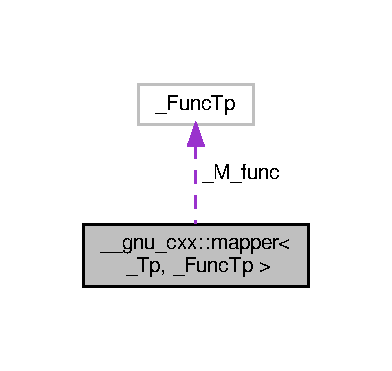
\includegraphics[width=188pt]{struct____gnu__cxx_1_1mapper__coll__graph}
\end{center}
\end{figure}
\subsection*{Public Member Functions}
\begin{DoxyCompactItemize}
\item 
\hyperlink{struct____gnu__cxx_1_1mapper_ae62b3c36179d502b8cf8ca670031d650}{mapper} (\+\_\+\+Func\+Tp \hyperlink{namespace____gnu__cxx_af2b2f0c7a2ae72b922b1afefae5a65b2}{\+\_\+\+\_\+func})
\end{DoxyCompactItemize}
\subsection*{Public Attributes}
\begin{DoxyCompactItemize}
\item 
\+\_\+\+Func\+Tp \hyperlink{struct____gnu__cxx_1_1mapper_a577a510fcb97643f3681a251a3a7acca}{\+\_\+\+M\+\_\+func}
\end{DoxyCompactItemize}


\subsection{Detailed Description}
\subsubsection*{template$<$typename \+\_\+\+Tp, typename \+\_\+\+Func\+Tp$>$\newline
struct \+\_\+\+\_\+gnu\+\_\+cxx\+::mapper$<$ \+\_\+\+Tp, \+\_\+\+Func\+Tp $>$}



Definition at line 29 of file integration\+\_\+transform.\+h.



\subsection{Constructor \& Destructor Documentation}
\mbox{\Hypertarget{struct____gnu__cxx_1_1mapper_ae62b3c36179d502b8cf8ca670031d650}\label{struct____gnu__cxx_1_1mapper_ae62b3c36179d502b8cf8ca670031d650}} 
\index{\+\_\+\+\_\+gnu\+\_\+cxx\+::mapper@{\+\_\+\+\_\+gnu\+\_\+cxx\+::mapper}!mapper@{mapper}}
\index{mapper@{mapper}!\+\_\+\+\_\+gnu\+\_\+cxx\+::mapper@{\+\_\+\+\_\+gnu\+\_\+cxx\+::mapper}}
\subsubsection{\texorpdfstring{mapper()}{mapper()}}
{\footnotesize\ttfamily template$<$typename \+\_\+\+Tp , typename \+\_\+\+Func\+Tp $>$ \\
\hyperlink{struct____gnu__cxx_1_1mapper}{\+\_\+\+\_\+gnu\+\_\+cxx\+::mapper}$<$ \hyperlink{namespace____gnu__cxx_a3b19a9c800ca194374ef9172290f7d79}{\+\_\+\+Tp}, \+\_\+\+Func\+Tp $>$\+::\hyperlink{struct____gnu__cxx_1_1mapper}{mapper} (\begin{DoxyParamCaption}\item[{\+\_\+\+Func\+Tp}]{\+\_\+\+\_\+func }\end{DoxyParamCaption})\hspace{0.3cm}{\ttfamily [inline]}}



Definition at line 33 of file integration\+\_\+transform.\+h.


\begin{DoxyCode}
34       : \hyperlink{struct____gnu__cxx_1_1mapper_a577a510fcb97643f3681a251a3a7acca}{\_M\_func}(\hyperlink{namespace____gnu__cxx_af2b2f0c7a2ae72b922b1afefae5a65b2}{\_\_func})
35       \{ \}
\end{DoxyCode}


\subsection{Member Data Documentation}
\mbox{\Hypertarget{struct____gnu__cxx_1_1mapper_a577a510fcb97643f3681a251a3a7acca}\label{struct____gnu__cxx_1_1mapper_a577a510fcb97643f3681a251a3a7acca}} 
\index{\+\_\+\+\_\+gnu\+\_\+cxx\+::mapper@{\+\_\+\+\_\+gnu\+\_\+cxx\+::mapper}!\+\_\+\+M\+\_\+func@{\+\_\+\+M\+\_\+func}}
\index{\+\_\+\+M\+\_\+func@{\+\_\+\+M\+\_\+func}!\+\_\+\+\_\+gnu\+\_\+cxx\+::mapper@{\+\_\+\+\_\+gnu\+\_\+cxx\+::mapper}}
\subsubsection{\texorpdfstring{\+\_\+\+M\+\_\+func}{\_M\_func}}
{\footnotesize\ttfamily template$<$typename \+\_\+\+Tp , typename \+\_\+\+Func\+Tp $>$ \\
\+\_\+\+Func\+Tp \hyperlink{struct____gnu__cxx_1_1mapper}{\+\_\+\+\_\+gnu\+\_\+cxx\+::mapper}$<$ \hyperlink{namespace____gnu__cxx_a3b19a9c800ca194374ef9172290f7d79}{\+\_\+\+Tp}, \+\_\+\+Func\+Tp $>$\+::\+\_\+\+M\+\_\+func}



Definition at line 31 of file integration\+\_\+transform.\+h.



Referenced by \+\_\+\+\_\+gnu\+\_\+cxx\+::map\+\_\+minf\+\_\+pinf\+\_\+symm$<$ \+\_\+\+Tp, \+\_\+\+Func\+Tp $>$\+::operator()(), \+\_\+\+\_\+gnu\+\_\+cxx\+::map\+\_\+minf\+\_\+pinf$<$ \+\_\+\+Tp, \+\_\+\+Func\+Tp $>$\+::operator()(), \+\_\+\+\_\+gnu\+\_\+cxx\+::map\+\_\+minf\+\_\+b$<$ \+\_\+\+Tp, \+\_\+\+Func\+Tp $>$\+::operator()(), and \+\_\+\+\_\+gnu\+\_\+cxx\+::map\+\_\+a\+\_\+pinf$<$ \+\_\+\+Tp, \+\_\+\+Func\+Tp $>$\+::operator()().



The documentation for this struct was generated from the following file\+:\begin{DoxyCompactItemize}
\item 
include/ext/\hyperlink{integration__transform_8h}{integration\+\_\+transform.\+h}\end{DoxyCompactItemize}

\hypertarget{class____gnu__cxx_1_1midpoint__integral}{}\section{\+\_\+\+\_\+gnu\+\_\+cxx\+:\+:midpoint\+\_\+integral$<$ \+\_\+\+Tp, \+\_\+\+Func\+Tp $>$ Class Template Reference}
\label{class____gnu__cxx_1_1midpoint__integral}\index{\+\_\+\+\_\+gnu\+\_\+cxx\+::midpoint\+\_\+integral$<$ \+\_\+\+Tp, \+\_\+\+Func\+Tp $>$@{\+\_\+\+\_\+gnu\+\_\+cxx\+::midpoint\+\_\+integral$<$ \+\_\+\+Tp, \+\_\+\+Func\+Tp $>$}}


{\ttfamily \#include $<$midpoint\+\_\+integral.\+h$>$}

\subsection*{Public Types}
\begin{DoxyCompactItemize}
\item 
using \hyperlink{class____gnu__cxx_1_1midpoint__integral_ae4c2b0cff4d7385e5c046ec4400bc69e}{\+\_\+\+Abs\+Area\+Tp} = decltype(std\+::abs(\hyperlink{class____gnu__cxx_1_1midpoint__integral_a43cd31237c2257dd657a2a84fd33dd69}{\+\_\+\+Area\+Tp}\{\}))
\item 
using \hyperlink{class____gnu__cxx_1_1midpoint__integral_a43cd31237c2257dd657a2a84fd33dd69}{\+\_\+\+Area\+Tp} = decltype(\hyperlink{class____gnu__cxx_1_1midpoint__integral_a9d6b6a3d38d137c3cc9f832a4f5da59f}{\+\_\+\+Ret\+Tp}\{\} $\ast$\hyperlink{namespace____gnu__cxx_a3b19a9c800ca194374ef9172290f7d79}{\+\_\+\+Tp}\{\})
\item 
using \hyperlink{class____gnu__cxx_1_1midpoint__integral_a9d6b6a3d38d137c3cc9f832a4f5da59f}{\+\_\+\+Ret\+Tp} = std\+::invoke\+\_\+result\+\_\+t$<$ \+\_\+\+Func\+Tp, \hyperlink{namespace____gnu__cxx_a3b19a9c800ca194374ef9172290f7d79}{\+\_\+\+Tp} $>$
\end{DoxyCompactItemize}
\subsection*{Public Member Functions}
\begin{DoxyCompactItemize}
\item 
\hyperlink{class____gnu__cxx_1_1midpoint__integral_ab62eec15eb135eb9027724a5367c89b9}{midpoint\+\_\+integral} (\+\_\+\+Func\+Tp \+\_\+\+\_\+fun, \hyperlink{namespace____gnu__cxx_a3b19a9c800ca194374ef9172290f7d79}{\+\_\+\+Tp} \+\_\+\+\_\+a, \hyperlink{namespace____gnu__cxx_a3b19a9c800ca194374ef9172290f7d79}{\+\_\+\+Tp} \+\_\+\+\_\+b, \hyperlink{namespace____gnu__cxx_a3b19a9c800ca194374ef9172290f7d79}{\+\_\+\+Tp} \+\_\+\+\_\+abs\+\_\+tol, \hyperlink{namespace____gnu__cxx_a3b19a9c800ca194374ef9172290f7d79}{\+\_\+\+Tp} \+\_\+\+\_\+rel\+\_\+tol)
\item 
\hyperlink{class____gnu__cxx_1_1midpoint__integral_ae4c2b0cff4d7385e5c046ec4400bc69e}{\+\_\+\+Abs\+Area\+Tp} \hyperlink{class____gnu__cxx_1_1midpoint__integral_a2a94b9b48126ac73821c1e38223bfc33}{abs\+\_\+error} () const
\item 
{\footnotesize template$<$typename \+\_\+\+Func\+Tp2 $>$ }\\\hyperlink{struct____gnu__cxx_1_1adaptive__integral__t}{adaptive\+\_\+integral\+\_\+t}$<$ \hyperlink{namespace____gnu__cxx_a3b19a9c800ca194374ef9172290f7d79}{\+\_\+\+Tp}, std\+::invoke\+\_\+result\+\_\+t$<$ \+\_\+\+Func\+Tp2, \hyperlink{namespace____gnu__cxx_a3b19a9c800ca194374ef9172290f7d79}{\+\_\+\+Tp} $>$ $>$ \hyperlink{class____gnu__cxx_1_1midpoint__integral_ae991ad240c41205cbe4e68ef59bc6ca8}{integrate} (\+\_\+\+Func\+Tp2 \+\_\+\+\_\+fun, \hyperlink{namespace____gnu__cxx_a3b19a9c800ca194374ef9172290f7d79}{\+\_\+\+Tp} \+\_\+\+\_\+a, \hyperlink{namespace____gnu__cxx_a3b19a9c800ca194374ef9172290f7d79}{\+\_\+\+Tp} \+\_\+\+\_\+b)
\item 
\hyperlink{class____gnu__cxx_1_1midpoint__integral_a43cd31237c2257dd657a2a84fd33dd69}{\+\_\+\+Area\+Tp} \hyperlink{class____gnu__cxx_1_1midpoint__integral_aed17a2e7f3970c07e8ed08262dfe5430}{operator()} ()
\item 
{\footnotesize template$<$typename \+\_\+\+Func\+Tp2 $>$ }\\\hyperlink{struct____gnu__cxx_1_1adaptive__integral__t}{adaptive\+\_\+integral\+\_\+t}$<$ \hyperlink{namespace____gnu__cxx_a3b19a9c800ca194374ef9172290f7d79}{\+\_\+\+Tp}, std\+::invoke\+\_\+result\+\_\+t$<$ \+\_\+\+Func\+Tp2, \hyperlink{namespace____gnu__cxx_a3b19a9c800ca194374ef9172290f7d79}{\+\_\+\+Tp} $>$ $>$ \hyperlink{class____gnu__cxx_1_1midpoint__integral_aecb7f4b62849fe4d6b8a0f5cb2c6319f}{operator()} (\+\_\+\+Func\+Tp2 \+\_\+\+\_\+fun, \hyperlink{namespace____gnu__cxx_a3b19a9c800ca194374ef9172290f7d79}{\+\_\+\+Tp} \+\_\+\+\_\+a, \hyperlink{namespace____gnu__cxx_a3b19a9c800ca194374ef9172290f7d79}{\+\_\+\+Tp} \+\_\+\+\_\+b)
\end{DoxyCompactItemize}


\subsection{Detailed Description}
\subsubsection*{template$<$typename \+\_\+\+Tp, typename \+\_\+\+Func\+Tp$>$\newline
class \+\_\+\+\_\+gnu\+\_\+cxx\+::midpoint\+\_\+integral$<$ \+\_\+\+Tp, \+\_\+\+Func\+Tp $>$}

A globally adaptive recursive midpoint integrator. 

Definition at line 73 of file midpoint\+\_\+integral.\+h.



\subsection{Member Typedef Documentation}
\mbox{\Hypertarget{class____gnu__cxx_1_1midpoint__integral_ae4c2b0cff4d7385e5c046ec4400bc69e}\label{class____gnu__cxx_1_1midpoint__integral_ae4c2b0cff4d7385e5c046ec4400bc69e}} 
\index{\+\_\+\+\_\+gnu\+\_\+cxx\+::midpoint\+\_\+integral@{\+\_\+\+\_\+gnu\+\_\+cxx\+::midpoint\+\_\+integral}!\+\_\+\+Abs\+Area\+Tp@{\+\_\+\+Abs\+Area\+Tp}}
\index{\+\_\+\+Abs\+Area\+Tp@{\+\_\+\+Abs\+Area\+Tp}!\+\_\+\+\_\+gnu\+\_\+cxx\+::midpoint\+\_\+integral@{\+\_\+\+\_\+gnu\+\_\+cxx\+::midpoint\+\_\+integral}}
\subsubsection{\texorpdfstring{\+\_\+\+Abs\+Area\+Tp}{\_AbsAreaTp}}
{\footnotesize\ttfamily template$<$typename \+\_\+\+Tp, typename \+\_\+\+Func\+Tp$>$ \\
using \hyperlink{class____gnu__cxx_1_1midpoint__integral}{\+\_\+\+\_\+gnu\+\_\+cxx\+::midpoint\+\_\+integral}$<$ \hyperlink{namespace____gnu__cxx_a3b19a9c800ca194374ef9172290f7d79}{\+\_\+\+Tp}, \+\_\+\+Func\+Tp $>$\+::\hyperlink{class____gnu__cxx_1_1midpoint__integral_ae4c2b0cff4d7385e5c046ec4400bc69e}{\+\_\+\+Abs\+Area\+Tp} =  decltype(std\+::abs(\hyperlink{class____gnu__cxx_1_1midpoint__integral_a43cd31237c2257dd657a2a84fd33dd69}{\+\_\+\+Area\+Tp}\{\}))}



Definition at line 79 of file midpoint\+\_\+integral.\+h.

\mbox{\Hypertarget{class____gnu__cxx_1_1midpoint__integral_a43cd31237c2257dd657a2a84fd33dd69}\label{class____gnu__cxx_1_1midpoint__integral_a43cd31237c2257dd657a2a84fd33dd69}} 
\index{\+\_\+\+\_\+gnu\+\_\+cxx\+::midpoint\+\_\+integral@{\+\_\+\+\_\+gnu\+\_\+cxx\+::midpoint\+\_\+integral}!\+\_\+\+Area\+Tp@{\+\_\+\+Area\+Tp}}
\index{\+\_\+\+Area\+Tp@{\+\_\+\+Area\+Tp}!\+\_\+\+\_\+gnu\+\_\+cxx\+::midpoint\+\_\+integral@{\+\_\+\+\_\+gnu\+\_\+cxx\+::midpoint\+\_\+integral}}
\subsubsection{\texorpdfstring{\+\_\+\+Area\+Tp}{\_AreaTp}}
{\footnotesize\ttfamily template$<$typename \+\_\+\+Tp, typename \+\_\+\+Func\+Tp$>$ \\
using \hyperlink{class____gnu__cxx_1_1midpoint__integral}{\+\_\+\+\_\+gnu\+\_\+cxx\+::midpoint\+\_\+integral}$<$ \hyperlink{namespace____gnu__cxx_a3b19a9c800ca194374ef9172290f7d79}{\+\_\+\+Tp}, \+\_\+\+Func\+Tp $>$\+::\hyperlink{class____gnu__cxx_1_1midpoint__integral_a43cd31237c2257dd657a2a84fd33dd69}{\+\_\+\+Area\+Tp} =  decltype(\hyperlink{class____gnu__cxx_1_1midpoint__integral_a9d6b6a3d38d137c3cc9f832a4f5da59f}{\+\_\+\+Ret\+Tp}\{\} $\ast$ \hyperlink{namespace____gnu__cxx_a3b19a9c800ca194374ef9172290f7d79}{\+\_\+\+Tp}\{\})}



Definition at line 78 of file midpoint\+\_\+integral.\+h.

\mbox{\Hypertarget{class____gnu__cxx_1_1midpoint__integral_a9d6b6a3d38d137c3cc9f832a4f5da59f}\label{class____gnu__cxx_1_1midpoint__integral_a9d6b6a3d38d137c3cc9f832a4f5da59f}} 
\index{\+\_\+\+\_\+gnu\+\_\+cxx\+::midpoint\+\_\+integral@{\+\_\+\+\_\+gnu\+\_\+cxx\+::midpoint\+\_\+integral}!\+\_\+\+Ret\+Tp@{\+\_\+\+Ret\+Tp}}
\index{\+\_\+\+Ret\+Tp@{\+\_\+\+Ret\+Tp}!\+\_\+\+\_\+gnu\+\_\+cxx\+::midpoint\+\_\+integral@{\+\_\+\+\_\+gnu\+\_\+cxx\+::midpoint\+\_\+integral}}
\subsubsection{\texorpdfstring{\+\_\+\+Ret\+Tp}{\_RetTp}}
{\footnotesize\ttfamily template$<$typename \+\_\+\+Tp, typename \+\_\+\+Func\+Tp$>$ \\
using \hyperlink{class____gnu__cxx_1_1midpoint__integral}{\+\_\+\+\_\+gnu\+\_\+cxx\+::midpoint\+\_\+integral}$<$ \hyperlink{namespace____gnu__cxx_a3b19a9c800ca194374ef9172290f7d79}{\+\_\+\+Tp}, \+\_\+\+Func\+Tp $>$\+::\hyperlink{class____gnu__cxx_1_1midpoint__integral_a9d6b6a3d38d137c3cc9f832a4f5da59f}{\+\_\+\+Ret\+Tp} =  std\+::invoke\+\_\+result\+\_\+t$<$\+\_\+\+Func\+Tp, \hyperlink{namespace____gnu__cxx_a3b19a9c800ca194374ef9172290f7d79}{\+\_\+\+Tp}$>$}



Definition at line 77 of file midpoint\+\_\+integral.\+h.



\subsection{Constructor \& Destructor Documentation}
\mbox{\Hypertarget{class____gnu__cxx_1_1midpoint__integral_ab62eec15eb135eb9027724a5367c89b9}\label{class____gnu__cxx_1_1midpoint__integral_ab62eec15eb135eb9027724a5367c89b9}} 
\index{\+\_\+\+\_\+gnu\+\_\+cxx\+::midpoint\+\_\+integral@{\+\_\+\+\_\+gnu\+\_\+cxx\+::midpoint\+\_\+integral}!midpoint\+\_\+integral@{midpoint\+\_\+integral}}
\index{midpoint\+\_\+integral@{midpoint\+\_\+integral}!\+\_\+\+\_\+gnu\+\_\+cxx\+::midpoint\+\_\+integral@{\+\_\+\+\_\+gnu\+\_\+cxx\+::midpoint\+\_\+integral}}
\subsubsection{\texorpdfstring{midpoint\+\_\+integral()}{midpoint\_integral()}}
{\footnotesize\ttfamily template$<$typename \+\_\+\+Tp, typename \+\_\+\+Func\+Tp$>$ \\
\hyperlink{class____gnu__cxx_1_1midpoint__integral}{\+\_\+\+\_\+gnu\+\_\+cxx\+::midpoint\+\_\+integral}$<$ \hyperlink{namespace____gnu__cxx_a3b19a9c800ca194374ef9172290f7d79}{\+\_\+\+Tp}, \+\_\+\+Func\+Tp $>$\+::\hyperlink{class____gnu__cxx_1_1midpoint__integral}{midpoint\+\_\+integral} (\begin{DoxyParamCaption}\item[{\+\_\+\+Func\+Tp}]{\+\_\+\+\_\+fun,  }\item[{\hyperlink{namespace____gnu__cxx_a3b19a9c800ca194374ef9172290f7d79}{\+\_\+\+Tp}}]{\+\_\+\+\_\+a,  }\item[{\hyperlink{namespace____gnu__cxx_a3b19a9c800ca194374ef9172290f7d79}{\+\_\+\+Tp}}]{\+\_\+\+\_\+b,  }\item[{\hyperlink{namespace____gnu__cxx_a3b19a9c800ca194374ef9172290f7d79}{\+\_\+\+Tp}}]{\+\_\+\+\_\+abs\+\_\+tol,  }\item[{\hyperlink{namespace____gnu__cxx_a3b19a9c800ca194374ef9172290f7d79}{\+\_\+\+Tp}}]{\+\_\+\+\_\+rel\+\_\+tol }\end{DoxyParamCaption})\hspace{0.3cm}{\ttfamily [inline]}}



Definition at line 81 of file midpoint\+\_\+integral.\+h.



References \+\_\+\+\_\+gnu\+\_\+cxx\+::composite\+\_\+midpoint\+\_\+integral$<$ \+\_\+\+Tp, \+\_\+\+Func\+Tp $>$\+::operator()().


\begin{DoxyCode}
83       : \_M\_fun(\_\_fun), \_M\_lower\_lim(\_\_a), \_M\_upper\_lim(\_\_b),
84         \_M\_abs\_tol(std::abs(\_\_abs\_tol)), \_M\_rel\_tol(std::abs(\_\_rel\_tol)),
85         \_M\_result(), \_M\_abs\_error()
86       \{ \}
\end{DoxyCode}


\subsection{Member Function Documentation}
\mbox{\Hypertarget{class____gnu__cxx_1_1midpoint__integral_a2a94b9b48126ac73821c1e38223bfc33}\label{class____gnu__cxx_1_1midpoint__integral_a2a94b9b48126ac73821c1e38223bfc33}} 
\index{\+\_\+\+\_\+gnu\+\_\+cxx\+::midpoint\+\_\+integral@{\+\_\+\+\_\+gnu\+\_\+cxx\+::midpoint\+\_\+integral}!abs\+\_\+error@{abs\+\_\+error}}
\index{abs\+\_\+error@{abs\+\_\+error}!\+\_\+\+\_\+gnu\+\_\+cxx\+::midpoint\+\_\+integral@{\+\_\+\+\_\+gnu\+\_\+cxx\+::midpoint\+\_\+integral}}
\subsubsection{\texorpdfstring{abs\+\_\+error()}{abs\_error()}}
{\footnotesize\ttfamily template$<$typename \+\_\+\+Tp, typename \+\_\+\+Func\+Tp$>$ \\
\hyperlink{class____gnu__cxx_1_1midpoint__integral_ae4c2b0cff4d7385e5c046ec4400bc69e}{\+\_\+\+Abs\+Area\+Tp} \hyperlink{class____gnu__cxx_1_1midpoint__integral}{\+\_\+\+\_\+gnu\+\_\+cxx\+::midpoint\+\_\+integral}$<$ \hyperlink{namespace____gnu__cxx_a3b19a9c800ca194374ef9172290f7d79}{\+\_\+\+Tp}, \+\_\+\+Func\+Tp $>$\+::abs\+\_\+error (\begin{DoxyParamCaption}{ }\end{DoxyParamCaption}) const\hspace{0.3cm}{\ttfamily [inline]}}



Definition at line 90 of file midpoint\+\_\+integral.\+h.



Referenced by \+\_\+\+\_\+gnu\+\_\+cxx\+::midpoint\+\_\+integral$<$ \+\_\+\+Tp, \+\_\+\+Func\+Tp $>$\+::integrate(), and \+\_\+\+\_\+gnu\+\_\+cxx\+::integrate\+\_\+midpoint().


\begin{DoxyCode}
91       \{ \textcolor{keywordflow}{return} this->\_M\_abs\_error; \}
\end{DoxyCode}
\mbox{\Hypertarget{class____gnu__cxx_1_1midpoint__integral_ae991ad240c41205cbe4e68ef59bc6ca8}\label{class____gnu__cxx_1_1midpoint__integral_ae991ad240c41205cbe4e68ef59bc6ca8}} 
\index{\+\_\+\+\_\+gnu\+\_\+cxx\+::midpoint\+\_\+integral@{\+\_\+\+\_\+gnu\+\_\+cxx\+::midpoint\+\_\+integral}!integrate@{integrate}}
\index{integrate@{integrate}!\+\_\+\+\_\+gnu\+\_\+cxx\+::midpoint\+\_\+integral@{\+\_\+\+\_\+gnu\+\_\+cxx\+::midpoint\+\_\+integral}}
\subsubsection{\texorpdfstring{integrate()}{integrate()}}
{\footnotesize\ttfamily template$<$typename \+\_\+\+Tp, typename \+\_\+\+Func\+Tp$>$ \\
template$<$typename \+\_\+\+Func\+Tp2 $>$ \\
\hyperlink{struct____gnu__cxx_1_1adaptive__integral__t}{adaptive\+\_\+integral\+\_\+t}$<$\hyperlink{namespace____gnu__cxx_a3b19a9c800ca194374ef9172290f7d79}{\+\_\+\+Tp}, std\+::invoke\+\_\+result\+\_\+t$<$\+\_\+\+Func\+Tp2, \hyperlink{namespace____gnu__cxx_a3b19a9c800ca194374ef9172290f7d79}{\+\_\+\+Tp}$>$ $>$ \hyperlink{class____gnu__cxx_1_1midpoint__integral}{\+\_\+\+\_\+gnu\+\_\+cxx\+::midpoint\+\_\+integral}$<$ \hyperlink{namespace____gnu__cxx_a3b19a9c800ca194374ef9172290f7d79}{\+\_\+\+Tp}, \+\_\+\+Func\+Tp $>$\+::integrate (\begin{DoxyParamCaption}\item[{\+\_\+\+Func\+Tp2}]{\+\_\+\+\_\+fun,  }\item[{\hyperlink{namespace____gnu__cxx_a3b19a9c800ca194374ef9172290f7d79}{\+\_\+\+Tp}}]{\+\_\+\+\_\+a,  }\item[{\hyperlink{namespace____gnu__cxx_a3b19a9c800ca194374ef9172290f7d79}{\+\_\+\+Tp}}]{\+\_\+\+\_\+b }\end{DoxyParamCaption})\hspace{0.3cm}{\ttfamily [inline]}}



Definition at line 95 of file midpoint\+\_\+integral.\+h.



References \+\_\+\+\_\+gnu\+\_\+cxx\+::midpoint\+\_\+integral$<$ \+\_\+\+Tp, \+\_\+\+Func\+Tp $>$\+::abs\+\_\+error().


\begin{DoxyCode}
96         \{
97           midpoint\_integral<\_FuncTp2, \_Tp>
98             \_\_mpi(\_\_fun, \_\_a, \_\_b,
99                   this->\_M\_abs\_tol, this->\_M\_rel\_tol);
100           \textcolor{keywordflow}{return} \{\_\_mpi(), \_\_mpi.abs\_error() \};
101         \}
\end{DoxyCode}
\mbox{\Hypertarget{class____gnu__cxx_1_1midpoint__integral_aed17a2e7f3970c07e8ed08262dfe5430}\label{class____gnu__cxx_1_1midpoint__integral_aed17a2e7f3970c07e8ed08262dfe5430}} 
\index{\+\_\+\+\_\+gnu\+\_\+cxx\+::midpoint\+\_\+integral@{\+\_\+\+\_\+gnu\+\_\+cxx\+::midpoint\+\_\+integral}!operator()@{operator()}}
\index{operator()@{operator()}!\+\_\+\+\_\+gnu\+\_\+cxx\+::midpoint\+\_\+integral@{\+\_\+\+\_\+gnu\+\_\+cxx\+::midpoint\+\_\+integral}}
\subsubsection{\texorpdfstring{operator()()}{operator()()}\hspace{0.1cm}{\footnotesize\ttfamily [1/2]}}
{\footnotesize\ttfamily template$<$typename \+\_\+\+Tp , typename \+\_\+\+Func\+Tp $>$ \\
\hyperlink{class____gnu__cxx_1_1midpoint__integral}{midpoint\+\_\+integral}$<$ \hyperlink{namespace____gnu__cxx_a3b19a9c800ca194374ef9172290f7d79}{\+\_\+\+Tp}, \+\_\+\+Func\+Tp $>$\+::\hyperlink{class____gnu__cxx_1_1midpoint__integral_a43cd31237c2257dd657a2a84fd33dd69}{\+\_\+\+Area\+Tp} \hyperlink{class____gnu__cxx_1_1midpoint__integral}{\+\_\+\+\_\+gnu\+\_\+cxx\+::midpoint\+\_\+integral}$<$ \hyperlink{namespace____gnu__cxx_a3b19a9c800ca194374ef9172290f7d79}{\+\_\+\+Tp}, \+\_\+\+Func\+Tp $>$\+::operator() (\begin{DoxyParamCaption}{ }\end{DoxyParamCaption})}

Integrate the function by naive subdivision. 

Definition at line 52 of file midpoint\+\_\+integral.\+tcc.



References \+\_\+\+\_\+gnu\+\_\+cxx\+::\+\_\+\+Tp.


\begin{DoxyCode}
53     \{
54       \textcolor{keyword}{auto} \_\_sum\_prev = this->\_M\_step();
55       \textcolor{keywordflow}{for} (std::size\_t \_\_j = 1; \_\_j < \_S\_max\_iter; ++\_\_j)
56         \{
57           \textcolor{keyword}{const} \textcolor{keyword}{auto} \_\_sum = this->\_M\_step();
58           this->\_M\_abs\_error = std::abs(\_\_sum - \_\_sum\_prev);
59           \textcolor{keywordflow}{if} (this->\_M\_abs\_error < this->\_M\_rel\_tol * std::abs(\_\_sum))
60             \textcolor{keywordflow}{return} \_\_sum;
61           \textcolor{keywordflow}{if} (\_\_j > 6
62               && std::abs(\_\_sum) < this->\_M\_rel\_tol
63               && std::abs(\_\_sum\_prev) < this->\_M\_rel\_tol )
64             \textcolor{keywordflow}{return} \_\_sum;
65           \_\_sum\_prev = \_\_sum;
66         \}
67       \textcolor{keywordflow}{return} \_\_sum\_prev;
68     \}
\end{DoxyCode}
\mbox{\Hypertarget{class____gnu__cxx_1_1midpoint__integral_aecb7f4b62849fe4d6b8a0f5cb2c6319f}\label{class____gnu__cxx_1_1midpoint__integral_aecb7f4b62849fe4d6b8a0f5cb2c6319f}} 
\index{\+\_\+\+\_\+gnu\+\_\+cxx\+::midpoint\+\_\+integral@{\+\_\+\+\_\+gnu\+\_\+cxx\+::midpoint\+\_\+integral}!operator()@{operator()}}
\index{operator()@{operator()}!\+\_\+\+\_\+gnu\+\_\+cxx\+::midpoint\+\_\+integral@{\+\_\+\+\_\+gnu\+\_\+cxx\+::midpoint\+\_\+integral}}
\subsubsection{\texorpdfstring{operator()()}{operator()()}\hspace{0.1cm}{\footnotesize\ttfamily [2/2]}}
{\footnotesize\ttfamily template$<$typename \+\_\+\+Tp, typename \+\_\+\+Func\+Tp$>$ \\
template$<$typename \+\_\+\+Func\+Tp2 $>$ \\
\hyperlink{struct____gnu__cxx_1_1adaptive__integral__t}{adaptive\+\_\+integral\+\_\+t}$<$\hyperlink{namespace____gnu__cxx_a3b19a9c800ca194374ef9172290f7d79}{\+\_\+\+Tp}, std\+::invoke\+\_\+result\+\_\+t$<$\+\_\+\+Func\+Tp2, \hyperlink{namespace____gnu__cxx_a3b19a9c800ca194374ef9172290f7d79}{\+\_\+\+Tp}$>$ $>$ \hyperlink{class____gnu__cxx_1_1midpoint__integral}{\+\_\+\+\_\+gnu\+\_\+cxx\+::midpoint\+\_\+integral}$<$ \hyperlink{namespace____gnu__cxx_a3b19a9c800ca194374ef9172290f7d79}{\+\_\+\+Tp}, \+\_\+\+Func\+Tp $>$\+::operator() (\begin{DoxyParamCaption}\item[{\+\_\+\+Func\+Tp2}]{\+\_\+\+\_\+fun,  }\item[{\hyperlink{namespace____gnu__cxx_a3b19a9c800ca194374ef9172290f7d79}{\+\_\+\+Tp}}]{\+\_\+\+\_\+a,  }\item[{\hyperlink{namespace____gnu__cxx_a3b19a9c800ca194374ef9172290f7d79}{\+\_\+\+Tp}}]{\+\_\+\+\_\+b }\end{DoxyParamCaption})\hspace{0.3cm}{\ttfamily [inline]}}



Definition at line 105 of file midpoint\+\_\+integral.\+h.



References \+\_\+\+\_\+gnu\+\_\+cxx\+::\+\_\+\+Tp, and \+\_\+\+\_\+gnu\+\_\+cxx\+::composite\+\_\+midpoint\+\_\+integral$<$ \+\_\+\+Tp, \+\_\+\+Func\+Tp $>$\+::integrate().


\begin{DoxyCode}
106         \{ \textcolor{keywordflow}{return} this->\hyperlink{class____gnu__cxx_1_1midpoint__integral_ae991ad240c41205cbe4e68ef59bc6ca8}{integrate}(\_\_fun, \_\_a, \_\_b); \}
\end{DoxyCode}


The documentation for this class was generated from the following files\+:\begin{DoxyCompactItemize}
\item 
include/ext/\hyperlink{midpoint__integral_8h}{midpoint\+\_\+integral.\+h}\item 
include/ext/\hyperlink{midpoint__integral_8tcc}{midpoint\+\_\+integral.\+tcc}\end{DoxyCompactItemize}

\hypertarget{struct____gnu__cxx_1_1oscillatory__integration__table}{}\section{\+\_\+\+\_\+gnu\+\_\+cxx\+:\+:oscillatory\+\_\+integration\+\_\+table$<$ \+\_\+\+Tp $>$ Struct Template Reference}
\label{struct____gnu__cxx_1_1oscillatory__integration__table}\index{\+\_\+\+\_\+gnu\+\_\+cxx\+::oscillatory\+\_\+integration\+\_\+table$<$ \+\_\+\+Tp $>$@{\+\_\+\+\_\+gnu\+\_\+cxx\+::oscillatory\+\_\+integration\+\_\+table$<$ \+\_\+\+Tp $>$}}


{\ttfamily \#include $<$oscillatory\+\_\+integration\+\_\+table.\+h$>$}



Collaboration diagram for \+\_\+\+\_\+gnu\+\_\+cxx\+:\+:oscillatory\+\_\+integration\+\_\+table$<$ \+\_\+\+Tp $>$\+:
\nopagebreak
\begin{figure}[H]
\begin{center}
\leavevmode
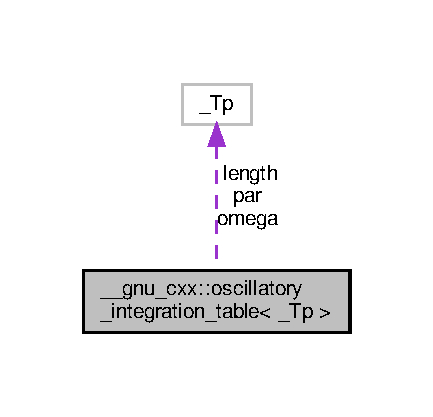
\includegraphics[width=208pt]{struct____gnu__cxx_1_1oscillatory__integration__table__coll__graph}
\end{center}
\end{figure}
\subsection*{Public Types}
\begin{DoxyCompactItemize}
\item 
enum \hyperlink{struct____gnu__cxx_1_1oscillatory__integration__table_aea06e472bb9ff6c535cfdc6a84b14e96}{circular\+\_\+function} \{ \hyperlink{struct____gnu__cxx_1_1oscillatory__integration__table_aea06e472bb9ff6c535cfdc6a84b14e96a4dc67b0a19d36f10e54840cb0cf397ef}{I\+N\+T\+E\+G\+\_\+\+C\+O\+S\+I\+NE}, 
\hyperlink{struct____gnu__cxx_1_1oscillatory__integration__table_aea06e472bb9ff6c535cfdc6a84b14e96a1714dec4721f5e596142c8a09f83a743}{I\+N\+T\+E\+G\+\_\+\+S\+I\+NE}
 \}
\end{DoxyCompactItemize}
\subsection*{Public Member Functions}
\begin{DoxyCompactItemize}
\item 
\hyperlink{struct____gnu__cxx_1_1oscillatory__integration__table_a0c69a8118986fe8c7de49d824ff26e1f}{oscillatory\+\_\+integration\+\_\+table} (\hyperlink{namespace____gnu__cxx_a3b19a9c800ca194374ef9172290f7d79}{\+\_\+\+Tp} omega\+\_\+in, \hyperlink{namespace____gnu__cxx_a3b19a9c800ca194374ef9172290f7d79}{\+\_\+\+Tp} length\+\_\+in, \hyperlink{struct____gnu__cxx_1_1oscillatory__integration__table_aea06e472bb9ff6c535cfdc6a84b14e96}{circular\+\_\+function} circfun\+\_\+in, std\+::size\+\_\+t n\+\_\+in)
\item 
\hyperlink{namespace____gnu__cxx_a3b19a9c800ca194374ef9172290f7d79}{\+\_\+\+Tp} \hyperlink{struct____gnu__cxx_1_1oscillatory__integration__table_a633fd01504b26abd2725d2d7e38c03c1}{get\+\_\+length} () const
\item 
const \hyperlink{namespace____gnu__cxx_a3b19a9c800ca194374ef9172290f7d79}{\+\_\+\+Tp} $\ast$ \hyperlink{struct____gnu__cxx_1_1oscillatory__integration__table_a7bb771c92944e0933bc90d7160cfb5be}{get\+\_\+moments} (std\+::size\+\_\+t \+\_\+\+\_\+level) const
\item 
void \hyperlink{struct____gnu__cxx_1_1oscillatory__integration__table_a6eac687c4e5dc65c8bf6626b24839975}{reset} (\hyperlink{namespace____gnu__cxx_a3b19a9c800ca194374ef9172290f7d79}{\+\_\+\+Tp} omega\+\_\+in, \hyperlink{namespace____gnu__cxx_a3b19a9c800ca194374ef9172290f7d79}{\+\_\+\+Tp} length\+\_\+in, \hyperlink{struct____gnu__cxx_1_1oscillatory__integration__table_aea06e472bb9ff6c535cfdc6a84b14e96}{circular\+\_\+function} circfun\+\_\+in)
\item 
\hyperlink{struct____gnu__cxx_1_1oscillatory__integration__table}{oscillatory\+\_\+integration\+\_\+table}$<$ \hyperlink{namespace____gnu__cxx_a3b19a9c800ca194374ef9172290f7d79}{\+\_\+\+Tp} $>$ \& \hyperlink{struct____gnu__cxx_1_1oscillatory__integration__table_a086da28f8232d48ed2a3257eba2aec4c}{set\+\_\+length} (\hyperlink{namespace____gnu__cxx_a3b19a9c800ca194374ef9172290f7d79}{\+\_\+\+Tp} length\+\_\+in)
\end{DoxyCompactItemize}
\subsection*{Public Attributes}
\begin{DoxyCompactItemize}
\item 
std\+::vector$<$ \hyperlink{namespace____gnu__cxx_a3b19a9c800ca194374ef9172290f7d79}{\+\_\+\+Tp} $>$ \hyperlink{struct____gnu__cxx_1_1oscillatory__integration__table_a29c973330c5f164962da57a528ccab55}{chebmo}
\item 
enum \hyperlink{struct____gnu__cxx_1_1oscillatory__integration__table_aea06e472bb9ff6c535cfdc6a84b14e96}{circular\+\_\+function} \hyperlink{struct____gnu__cxx_1_1oscillatory__integration__table_a21f86f96ca3654c18fa987f15bc14eaf}{circfun}
\item 
\hyperlink{namespace____gnu__cxx_a3b19a9c800ca194374ef9172290f7d79}{\+\_\+\+Tp} \hyperlink{struct____gnu__cxx_1_1oscillatory__integration__table_ad8654aa233b4878af8d9a99ed61db488}{length}
\item 
std\+::size\+\_\+t \hyperlink{struct____gnu__cxx_1_1oscillatory__integration__table_a7afb6e15c7cf51c48ed89fc2d8450179}{n}
\item 
\hyperlink{namespace____gnu__cxx_a3b19a9c800ca194374ef9172290f7d79}{\+\_\+\+Tp} \hyperlink{struct____gnu__cxx_1_1oscillatory__integration__table_a722a28c43e85cce33bbe6337e6a5c9eb}{omega}
\item 
\hyperlink{namespace____gnu__cxx_a3b19a9c800ca194374ef9172290f7d79}{\+\_\+\+Tp} \hyperlink{struct____gnu__cxx_1_1oscillatory__integration__table_ae98255b8cccea27dde0047c45cfc2ac6}{par}
\end{DoxyCompactItemize}


\subsection{Detailed Description}
\subsubsection*{template$<$typename \+\_\+\+Tp$>$\newline
struct \+\_\+\+\_\+gnu\+\_\+cxx\+::oscillatory\+\_\+integration\+\_\+table$<$ \+\_\+\+Tp $>$}



Definition at line 35 of file oscillatory\+\_\+integration\+\_\+table.\+h.



\subsection{Member Enumeration Documentation}
\mbox{\Hypertarget{struct____gnu__cxx_1_1oscillatory__integration__table_aea06e472bb9ff6c535cfdc6a84b14e96}\label{struct____gnu__cxx_1_1oscillatory__integration__table_aea06e472bb9ff6c535cfdc6a84b14e96}} 
\index{\+\_\+\+\_\+gnu\+\_\+cxx\+::oscillatory\+\_\+integration\+\_\+table@{\+\_\+\+\_\+gnu\+\_\+cxx\+::oscillatory\+\_\+integration\+\_\+table}!circular\+\_\+function@{circular\+\_\+function}}
\index{circular\+\_\+function@{circular\+\_\+function}!\+\_\+\+\_\+gnu\+\_\+cxx\+::oscillatory\+\_\+integration\+\_\+table@{\+\_\+\+\_\+gnu\+\_\+cxx\+::oscillatory\+\_\+integration\+\_\+table}}
\subsubsection{\texorpdfstring{circular\+\_\+function}{circular\_function}}
{\footnotesize\ttfamily template$<$typename \+\_\+\+Tp$>$ \\
enum \hyperlink{struct____gnu__cxx_1_1oscillatory__integration__table_aea06e472bb9ff6c535cfdc6a84b14e96}{\+\_\+\+\_\+gnu\+\_\+cxx\+::oscillatory\+\_\+integration\+\_\+table\+::circular\+\_\+function}}

\begin{DoxyEnumFields}{Enumerator}
\raisebox{\heightof{T}}[0pt][0pt]{\index{I\+N\+T\+E\+G\+\_\+\+C\+O\+S\+I\+NE@{I\+N\+T\+E\+G\+\_\+\+C\+O\+S\+I\+NE}!\+\_\+\+\_\+gnu\+\_\+cxx\+::oscillatory\+\_\+integration\+\_\+table@{\+\_\+\+\_\+gnu\+\_\+cxx\+::oscillatory\+\_\+integration\+\_\+table}}\index{\+\_\+\+\_\+gnu\+\_\+cxx\+::oscillatory\+\_\+integration\+\_\+table@{\+\_\+\+\_\+gnu\+\_\+cxx\+::oscillatory\+\_\+integration\+\_\+table}!I\+N\+T\+E\+G\+\_\+\+C\+O\+S\+I\+NE@{I\+N\+T\+E\+G\+\_\+\+C\+O\+S\+I\+NE}}}\mbox{\Hypertarget{struct____gnu__cxx_1_1oscillatory__integration__table_aea06e472bb9ff6c535cfdc6a84b14e96a4dc67b0a19d36f10e54840cb0cf397ef}\label{struct____gnu__cxx_1_1oscillatory__integration__table_aea06e472bb9ff6c535cfdc6a84b14e96a4dc67b0a19d36f10e54840cb0cf397ef}} 
I\+N\+T\+E\+G\+\_\+\+C\+O\+S\+I\+NE&\\
\hline

\raisebox{\heightof{T}}[0pt][0pt]{\index{I\+N\+T\+E\+G\+\_\+\+S\+I\+NE@{I\+N\+T\+E\+G\+\_\+\+S\+I\+NE}!\+\_\+\+\_\+gnu\+\_\+cxx\+::oscillatory\+\_\+integration\+\_\+table@{\+\_\+\+\_\+gnu\+\_\+cxx\+::oscillatory\+\_\+integration\+\_\+table}}\index{\+\_\+\+\_\+gnu\+\_\+cxx\+::oscillatory\+\_\+integration\+\_\+table@{\+\_\+\+\_\+gnu\+\_\+cxx\+::oscillatory\+\_\+integration\+\_\+table}!I\+N\+T\+E\+G\+\_\+\+S\+I\+NE@{I\+N\+T\+E\+G\+\_\+\+S\+I\+NE}}}\mbox{\Hypertarget{struct____gnu__cxx_1_1oscillatory__integration__table_aea06e472bb9ff6c535cfdc6a84b14e96a1714dec4721f5e596142c8a09f83a743}\label{struct____gnu__cxx_1_1oscillatory__integration__table_aea06e472bb9ff6c535cfdc6a84b14e96a1714dec4721f5e596142c8a09f83a743}} 
I\+N\+T\+E\+G\+\_\+\+S\+I\+NE&\\
\hline

\end{DoxyEnumFields}


Definition at line 37 of file oscillatory\+\_\+integration\+\_\+table.\+h.


\begin{DoxyCode}
38       \{
39         \hyperlink{struct____gnu__cxx_1_1oscillatory__integration__table_aea06e472bb9ff6c535cfdc6a84b14e96a4dc67b0a19d36f10e54840cb0cf397ef}{INTEG\_COSINE},
40         \hyperlink{struct____gnu__cxx_1_1oscillatory__integration__table_aea06e472bb9ff6c535cfdc6a84b14e96a1714dec4721f5e596142c8a09f83a743}{INTEG\_SINE}
41       \};
\end{DoxyCode}


\subsection{Constructor \& Destructor Documentation}
\mbox{\Hypertarget{struct____gnu__cxx_1_1oscillatory__integration__table_a0c69a8118986fe8c7de49d824ff26e1f}\label{struct____gnu__cxx_1_1oscillatory__integration__table_a0c69a8118986fe8c7de49d824ff26e1f}} 
\index{\+\_\+\+\_\+gnu\+\_\+cxx\+::oscillatory\+\_\+integration\+\_\+table@{\+\_\+\+\_\+gnu\+\_\+cxx\+::oscillatory\+\_\+integration\+\_\+table}!oscillatory\+\_\+integration\+\_\+table@{oscillatory\+\_\+integration\+\_\+table}}
\index{oscillatory\+\_\+integration\+\_\+table@{oscillatory\+\_\+integration\+\_\+table}!\+\_\+\+\_\+gnu\+\_\+cxx\+::oscillatory\+\_\+integration\+\_\+table@{\+\_\+\+\_\+gnu\+\_\+cxx\+::oscillatory\+\_\+integration\+\_\+table}}
\subsubsection{\texorpdfstring{oscillatory\+\_\+integration\+\_\+table()}{oscillatory\_integration\_table()}}
{\footnotesize\ttfamily template$<$typename \+\_\+\+Tp$>$ \\
\hyperlink{struct____gnu__cxx_1_1oscillatory__integration__table}{\+\_\+\+\_\+gnu\+\_\+cxx\+::oscillatory\+\_\+integration\+\_\+table}$<$ \hyperlink{namespace____gnu__cxx_a3b19a9c800ca194374ef9172290f7d79}{\+\_\+\+Tp} $>$\+::\hyperlink{struct____gnu__cxx_1_1oscillatory__integration__table}{oscillatory\+\_\+integration\+\_\+table} (\begin{DoxyParamCaption}\item[{\hyperlink{namespace____gnu__cxx_a3b19a9c800ca194374ef9172290f7d79}{\+\_\+\+Tp}}]{omega\+\_\+in,  }\item[{\hyperlink{namespace____gnu__cxx_a3b19a9c800ca194374ef9172290f7d79}{\+\_\+\+Tp}}]{length\+\_\+in,  }\item[{\hyperlink{struct____gnu__cxx_1_1oscillatory__integration__table_aea06e472bb9ff6c535cfdc6a84b14e96}{circular\+\_\+function}}]{circfun\+\_\+in,  }\item[{std\+::size\+\_\+t}]{n\+\_\+in }\end{DoxyParamCaption})\hspace{0.3cm}{\ttfamily [inline]}}



Definition at line 50 of file oscillatory\+\_\+integration\+\_\+table.\+h.



References \+\_\+\+\_\+gnu\+\_\+cxx\+::\+\_\+\+Tp, and \+\_\+\+\_\+gnu\+\_\+cxx\+::oscillatory\+\_\+integration\+\_\+table$<$ \+\_\+\+Tp $>$\+::n.


\begin{DoxyCode}
53       : \hyperlink{struct____gnu__cxx_1_1oscillatory__integration__table_a7afb6e15c7cf51c48ed89fc2d8450179}{n}(n\_in),
54         \hyperlink{struct____gnu__cxx_1_1oscillatory__integration__table_a722a28c43e85cce33bbe6337e6a5c9eb}{omega}(omega\_in),
55         \hyperlink{struct____gnu__cxx_1_1oscillatory__integration__table_ad8654aa233b4878af8d9a99ed61db488}{length}(length\_in),
56         \hyperlink{struct____gnu__cxx_1_1oscillatory__integration__table_ae98255b8cccea27dde0047c45cfc2ac6}{par}(0.5 * omega\_in * length\_in),
57         \hyperlink{struct____gnu__cxx_1_1oscillatory__integration__table_a21f86f96ca3654c18fa987f15bc14eaf}{circfun}(circfun\_in),
58         \hyperlink{struct____gnu__cxx_1_1oscillatory__integration__table_a29c973330c5f164962da57a528ccab55}{chebmo}(25 * n\_in)
59       \{
60         \textcolor{keyword}{auto} \_\_scale = \hyperlink{namespace____gnu__cxx_a3b19a9c800ca194374ef9172290f7d79}{\_Tp}\{1\};
61         \textcolor{keywordflow}{for} (\textcolor{keyword}{auto} \_\_i = 0u; \_\_i < this->\hyperlink{struct____gnu__cxx_1_1oscillatory__integration__table_a7afb6e15c7cf51c48ed89fc2d8450179}{n}; ++\_\_i)
62           \{
63             this->compute\_moments(this->\hyperlink{struct____gnu__cxx_1_1oscillatory__integration__table_ae98255b8cccea27dde0047c45cfc2ac6}{par} * \_\_scale, \_\_i);
64             \_\_scale *= 0.5;
65             \textcolor{comment}{// Prevent divide by zero.}
66             \textcolor{keywordflow}{if} (\textcolor{keyword}{const} \textcolor{keyword}{auto} \_\_scale2 = \_\_scale * \_\_scale;
67                 \_\_scale2 * \_\_scale2 == \hyperlink{namespace____gnu__cxx_a3b19a9c800ca194374ef9172290f7d79}{\_Tp}\{0\})
68               \{
69                 this->n = \_\_i;
70                 \textcolor{keywordflow}{break};
71               \}
72           \}
73       \}
\end{DoxyCode}


\subsection{Member Function Documentation}
\mbox{\Hypertarget{struct____gnu__cxx_1_1oscillatory__integration__table_a633fd01504b26abd2725d2d7e38c03c1}\label{struct____gnu__cxx_1_1oscillatory__integration__table_a633fd01504b26abd2725d2d7e38c03c1}} 
\index{\+\_\+\+\_\+gnu\+\_\+cxx\+::oscillatory\+\_\+integration\+\_\+table@{\+\_\+\+\_\+gnu\+\_\+cxx\+::oscillatory\+\_\+integration\+\_\+table}!get\+\_\+length@{get\+\_\+length}}
\index{get\+\_\+length@{get\+\_\+length}!\+\_\+\+\_\+gnu\+\_\+cxx\+::oscillatory\+\_\+integration\+\_\+table@{\+\_\+\+\_\+gnu\+\_\+cxx\+::oscillatory\+\_\+integration\+\_\+table}}
\subsubsection{\texorpdfstring{get\+\_\+length()}{get\_length()}}
{\footnotesize\ttfamily template$<$typename \+\_\+\+Tp$>$ \\
\hyperlink{namespace____gnu__cxx_a3b19a9c800ca194374ef9172290f7d79}{\+\_\+\+Tp} \hyperlink{struct____gnu__cxx_1_1oscillatory__integration__table}{\+\_\+\+\_\+gnu\+\_\+cxx\+::oscillatory\+\_\+integration\+\_\+table}$<$ \hyperlink{namespace____gnu__cxx_a3b19a9c800ca194374ef9172290f7d79}{\+\_\+\+Tp} $>$\+::get\+\_\+length (\begin{DoxyParamCaption}{ }\end{DoxyParamCaption}) const\hspace{0.3cm}{\ttfamily [inline]}}



Definition at line 76 of file oscillatory\+\_\+integration\+\_\+table.\+h.



References \+\_\+\+\_\+gnu\+\_\+cxx\+::oscillatory\+\_\+integration\+\_\+table$<$ \+\_\+\+Tp $>$\+::length.


\begin{DoxyCode}
77       \{ \textcolor{keywordflow}{return} this->\hyperlink{struct____gnu__cxx_1_1oscillatory__integration__table_ad8654aa233b4878af8d9a99ed61db488}{length}; \}
\end{DoxyCode}
\mbox{\Hypertarget{struct____gnu__cxx_1_1oscillatory__integration__table_a7bb771c92944e0933bc90d7160cfb5be}\label{struct____gnu__cxx_1_1oscillatory__integration__table_a7bb771c92944e0933bc90d7160cfb5be}} 
\index{\+\_\+\+\_\+gnu\+\_\+cxx\+::oscillatory\+\_\+integration\+\_\+table@{\+\_\+\+\_\+gnu\+\_\+cxx\+::oscillatory\+\_\+integration\+\_\+table}!get\+\_\+moments@{get\+\_\+moments}}
\index{get\+\_\+moments@{get\+\_\+moments}!\+\_\+\+\_\+gnu\+\_\+cxx\+::oscillatory\+\_\+integration\+\_\+table@{\+\_\+\+\_\+gnu\+\_\+cxx\+::oscillatory\+\_\+integration\+\_\+table}}
\subsubsection{\texorpdfstring{get\+\_\+moments()}{get\_moments()}}
{\footnotesize\ttfamily template$<$typename \+\_\+\+Tp$>$ \\
const \hyperlink{namespace____gnu__cxx_a3b19a9c800ca194374ef9172290f7d79}{\+\_\+\+Tp}$\ast$ \hyperlink{struct____gnu__cxx_1_1oscillatory__integration__table}{\+\_\+\+\_\+gnu\+\_\+cxx\+::oscillatory\+\_\+integration\+\_\+table}$<$ \hyperlink{namespace____gnu__cxx_a3b19a9c800ca194374ef9172290f7d79}{\+\_\+\+Tp} $>$\+::get\+\_\+moments (\begin{DoxyParamCaption}\item[{std\+::size\+\_\+t}]{\+\_\+\+\_\+level }\end{DoxyParamCaption}) const\hspace{0.3cm}{\ttfamily [inline]}}



Definition at line 105 of file oscillatory\+\_\+integration\+\_\+table.\+h.



References \+\_\+\+\_\+gnu\+\_\+cxx\+::\+\_\+\+Tp.


\begin{DoxyCode}
106       \{ \textcolor{keywordflow}{return} this->\hyperlink{struct____gnu__cxx_1_1oscillatory__integration__table_a29c973330c5f164962da57a528ccab55}{chebmo}.data() + 25 * \_\_level; \}
\end{DoxyCode}
\mbox{\Hypertarget{struct____gnu__cxx_1_1oscillatory__integration__table_a6eac687c4e5dc65c8bf6626b24839975}\label{struct____gnu__cxx_1_1oscillatory__integration__table_a6eac687c4e5dc65c8bf6626b24839975}} 
\index{\+\_\+\+\_\+gnu\+\_\+cxx\+::oscillatory\+\_\+integration\+\_\+table@{\+\_\+\+\_\+gnu\+\_\+cxx\+::oscillatory\+\_\+integration\+\_\+table}!reset@{reset}}
\index{reset@{reset}!\+\_\+\+\_\+gnu\+\_\+cxx\+::oscillatory\+\_\+integration\+\_\+table@{\+\_\+\+\_\+gnu\+\_\+cxx\+::oscillatory\+\_\+integration\+\_\+table}}
\subsubsection{\texorpdfstring{reset()}{reset()}}
{\footnotesize\ttfamily template$<$typename \+\_\+\+Tp$>$ \\
void \hyperlink{struct____gnu__cxx_1_1oscillatory__integration__table}{\+\_\+\+\_\+gnu\+\_\+cxx\+::oscillatory\+\_\+integration\+\_\+table}$<$ \hyperlink{namespace____gnu__cxx_a3b19a9c800ca194374ef9172290f7d79}{\+\_\+\+Tp} $>$\+::reset (\begin{DoxyParamCaption}\item[{\hyperlink{namespace____gnu__cxx_a3b19a9c800ca194374ef9172290f7d79}{\+\_\+\+Tp}}]{omega\+\_\+in,  }\item[{\hyperlink{namespace____gnu__cxx_a3b19a9c800ca194374ef9172290f7d79}{\+\_\+\+Tp}}]{length\+\_\+in,  }\item[{\hyperlink{struct____gnu__cxx_1_1oscillatory__integration__table_aea06e472bb9ff6c535cfdc6a84b14e96}{circular\+\_\+function}}]{circfun\+\_\+in }\end{DoxyParamCaption})\hspace{0.3cm}{\ttfamily [inline]}}



Definition at line 89 of file oscillatory\+\_\+integration\+\_\+table.\+h.



References \+\_\+\+\_\+gnu\+\_\+cxx\+::\+\_\+\+Tp, and \+\_\+\+\_\+gnu\+\_\+cxx\+::oscillatory\+\_\+integration\+\_\+table$<$ \+\_\+\+Tp $>$\+::n.



Referenced by \+\_\+\+\_\+gnu\+\_\+cxx\+::oscillatory\+\_\+integration\+\_\+table$<$ \+\_\+\+Tp $>$\+::set\+\_\+length().


\begin{DoxyCode}
91       \{
92         this->\hyperlink{struct____gnu__cxx_1_1oscillatory__integration__table_a722a28c43e85cce33bbe6337e6a5c9eb}{omega} = omega\_in;
93         this->\hyperlink{struct____gnu__cxx_1_1oscillatory__integration__table_ad8654aa233b4878af8d9a99ed61db488}{length} = length\_in;
94         this->\hyperlink{struct____gnu__cxx_1_1oscillatory__integration__table_ae98255b8cccea27dde0047c45cfc2ac6}{par} = 0.5 * omega\_in * length\_in;
95         this->\hyperlink{struct____gnu__cxx_1_1oscillatory__integration__table_a21f86f96ca3654c18fa987f15bc14eaf}{circfun} = circfun\_in;
96         \textcolor{keyword}{auto} \_\_scale = \hyperlink{namespace____gnu__cxx_a3b19a9c800ca194374ef9172290f7d79}{\_Tp}\{1\};
97         \textcolor{keywordflow}{for} (\textcolor{keyword}{auto} \_\_i = 0u; \_\_i < this->\hyperlink{struct____gnu__cxx_1_1oscillatory__integration__table_a7afb6e15c7cf51c48ed89fc2d8450179}{n}; ++\_\_i)
98           \{
99             this->compute\_moments(this->\hyperlink{struct____gnu__cxx_1_1oscillatory__integration__table_ae98255b8cccea27dde0047c45cfc2ac6}{par} * \_\_scale, \_\_i);
100             \_\_scale *= 0.5;
101           \}
102       \}
\end{DoxyCode}
\mbox{\Hypertarget{struct____gnu__cxx_1_1oscillatory__integration__table_a086da28f8232d48ed2a3257eba2aec4c}\label{struct____gnu__cxx_1_1oscillatory__integration__table_a086da28f8232d48ed2a3257eba2aec4c}} 
\index{\+\_\+\+\_\+gnu\+\_\+cxx\+::oscillatory\+\_\+integration\+\_\+table@{\+\_\+\+\_\+gnu\+\_\+cxx\+::oscillatory\+\_\+integration\+\_\+table}!set\+\_\+length@{set\+\_\+length}}
\index{set\+\_\+length@{set\+\_\+length}!\+\_\+\+\_\+gnu\+\_\+cxx\+::oscillatory\+\_\+integration\+\_\+table@{\+\_\+\+\_\+gnu\+\_\+cxx\+::oscillatory\+\_\+integration\+\_\+table}}
\subsubsection{\texorpdfstring{set\+\_\+length()}{set\_length()}}
{\footnotesize\ttfamily template$<$typename \+\_\+\+Tp$>$ \\
\hyperlink{struct____gnu__cxx_1_1oscillatory__integration__table}{oscillatory\+\_\+integration\+\_\+table}$<$\hyperlink{namespace____gnu__cxx_a3b19a9c800ca194374ef9172290f7d79}{\+\_\+\+Tp}$>$\& \hyperlink{struct____gnu__cxx_1_1oscillatory__integration__table}{\+\_\+\+\_\+gnu\+\_\+cxx\+::oscillatory\+\_\+integration\+\_\+table}$<$ \hyperlink{namespace____gnu__cxx_a3b19a9c800ca194374ef9172290f7d79}{\+\_\+\+Tp} $>$\+::set\+\_\+length (\begin{DoxyParamCaption}\item[{\hyperlink{namespace____gnu__cxx_a3b19a9c800ca194374ef9172290f7d79}{\+\_\+\+Tp}}]{length\+\_\+in }\end{DoxyParamCaption})\hspace{0.3cm}{\ttfamily [inline]}}



Definition at line 80 of file oscillatory\+\_\+integration\+\_\+table.\+h.



References \+\_\+\+\_\+gnu\+\_\+cxx\+::oscillatory\+\_\+integration\+\_\+table$<$ \+\_\+\+Tp $>$\+::length, and \+\_\+\+\_\+gnu\+\_\+cxx\+::oscillatory\+\_\+integration\+\_\+table$<$ \+\_\+\+Tp $>$\+::reset().


\begin{DoxyCode}
81       \{
82         this->\hyperlink{struct____gnu__cxx_1_1oscillatory__integration__table_ad8654aa233b4878af8d9a99ed61db488}{length} = length\_in;
83         this->\hyperlink{struct____gnu__cxx_1_1oscillatory__integration__table_ae98255b8cccea27dde0047c45cfc2ac6}{par} = 0.5 * this->\hyperlink{struct____gnu__cxx_1_1oscillatory__integration__table_a722a28c43e85cce33bbe6337e6a5c9eb}{omega} * this->\hyperlink{struct____gnu__cxx_1_1oscillatory__integration__table_ad8654aa233b4878af8d9a99ed61db488}{length};
84         this->\hyperlink{struct____gnu__cxx_1_1oscillatory__integration__table_a6eac687c4e5dc65c8bf6626b24839975}{reset}(this->\hyperlink{struct____gnu__cxx_1_1oscillatory__integration__table_a722a28c43e85cce33bbe6337e6a5c9eb}{omega}, this->length, this->\hyperlink{struct____gnu__cxx_1_1oscillatory__integration__table_a21f86f96ca3654c18fa987f15bc14eaf}{circfun});
85         \textcolor{keywordflow}{return} *\textcolor{keyword}{this};
86       \}
\end{DoxyCode}


\subsection{Member Data Documentation}
\mbox{\Hypertarget{struct____gnu__cxx_1_1oscillatory__integration__table_a29c973330c5f164962da57a528ccab55}\label{struct____gnu__cxx_1_1oscillatory__integration__table_a29c973330c5f164962da57a528ccab55}} 
\index{\+\_\+\+\_\+gnu\+\_\+cxx\+::oscillatory\+\_\+integration\+\_\+table@{\+\_\+\+\_\+gnu\+\_\+cxx\+::oscillatory\+\_\+integration\+\_\+table}!chebmo@{chebmo}}
\index{chebmo@{chebmo}!\+\_\+\+\_\+gnu\+\_\+cxx\+::oscillatory\+\_\+integration\+\_\+table@{\+\_\+\+\_\+gnu\+\_\+cxx\+::oscillatory\+\_\+integration\+\_\+table}}
\subsubsection{\texorpdfstring{chebmo}{chebmo}}
{\footnotesize\ttfamily template$<$typename \+\_\+\+Tp$>$ \\
std\+::vector$<$\hyperlink{namespace____gnu__cxx_a3b19a9c800ca194374ef9172290f7d79}{\+\_\+\+Tp}$>$ \hyperlink{struct____gnu__cxx_1_1oscillatory__integration__table}{\+\_\+\+\_\+gnu\+\_\+cxx\+::oscillatory\+\_\+integration\+\_\+table}$<$ \hyperlink{namespace____gnu__cxx_a3b19a9c800ca194374ef9172290f7d79}{\+\_\+\+Tp} $>$\+::chebmo}



Definition at line 48 of file oscillatory\+\_\+integration\+\_\+table.\+h.

\mbox{\Hypertarget{struct____gnu__cxx_1_1oscillatory__integration__table_a21f86f96ca3654c18fa987f15bc14eaf}\label{struct____gnu__cxx_1_1oscillatory__integration__table_a21f86f96ca3654c18fa987f15bc14eaf}} 
\index{\+\_\+\+\_\+gnu\+\_\+cxx\+::oscillatory\+\_\+integration\+\_\+table@{\+\_\+\+\_\+gnu\+\_\+cxx\+::oscillatory\+\_\+integration\+\_\+table}!circfun@{circfun}}
\index{circfun@{circfun}!\+\_\+\+\_\+gnu\+\_\+cxx\+::oscillatory\+\_\+integration\+\_\+table@{\+\_\+\+\_\+gnu\+\_\+cxx\+::oscillatory\+\_\+integration\+\_\+table}}
\subsubsection{\texorpdfstring{circfun}{circfun}}
{\footnotesize\ttfamily template$<$typename \+\_\+\+Tp$>$ \\
enum \hyperlink{struct____gnu__cxx_1_1oscillatory__integration__table_aea06e472bb9ff6c535cfdc6a84b14e96}{circular\+\_\+function} \hyperlink{struct____gnu__cxx_1_1oscillatory__integration__table}{\+\_\+\+\_\+gnu\+\_\+cxx\+::oscillatory\+\_\+integration\+\_\+table}$<$ \hyperlink{namespace____gnu__cxx_a3b19a9c800ca194374ef9172290f7d79}{\+\_\+\+Tp} $>$\+::circfun}



Definition at line 47 of file oscillatory\+\_\+integration\+\_\+table.\+h.

\mbox{\Hypertarget{struct____gnu__cxx_1_1oscillatory__integration__table_ad8654aa233b4878af8d9a99ed61db488}\label{struct____gnu__cxx_1_1oscillatory__integration__table_ad8654aa233b4878af8d9a99ed61db488}} 
\index{\+\_\+\+\_\+gnu\+\_\+cxx\+::oscillatory\+\_\+integration\+\_\+table@{\+\_\+\+\_\+gnu\+\_\+cxx\+::oscillatory\+\_\+integration\+\_\+table}!length@{length}}
\index{length@{length}!\+\_\+\+\_\+gnu\+\_\+cxx\+::oscillatory\+\_\+integration\+\_\+table@{\+\_\+\+\_\+gnu\+\_\+cxx\+::oscillatory\+\_\+integration\+\_\+table}}
\subsubsection{\texorpdfstring{length}{length}}
{\footnotesize\ttfamily template$<$typename \+\_\+\+Tp$>$ \\
\hyperlink{namespace____gnu__cxx_a3b19a9c800ca194374ef9172290f7d79}{\+\_\+\+Tp} \hyperlink{struct____gnu__cxx_1_1oscillatory__integration__table}{\+\_\+\+\_\+gnu\+\_\+cxx\+::oscillatory\+\_\+integration\+\_\+table}$<$ \hyperlink{namespace____gnu__cxx_a3b19a9c800ca194374ef9172290f7d79}{\+\_\+\+Tp} $>$\+::length}



Definition at line 45 of file oscillatory\+\_\+integration\+\_\+table.\+h.



Referenced by \+\_\+\+\_\+gnu\+\_\+cxx\+::oscillatory\+\_\+integration\+\_\+table$<$ \+\_\+\+Tp $>$\+::get\+\_\+length(), and \+\_\+\+\_\+gnu\+\_\+cxx\+::oscillatory\+\_\+integration\+\_\+table$<$ \+\_\+\+Tp $>$\+::set\+\_\+length().

\mbox{\Hypertarget{struct____gnu__cxx_1_1oscillatory__integration__table_a7afb6e15c7cf51c48ed89fc2d8450179}\label{struct____gnu__cxx_1_1oscillatory__integration__table_a7afb6e15c7cf51c48ed89fc2d8450179}} 
\index{\+\_\+\+\_\+gnu\+\_\+cxx\+::oscillatory\+\_\+integration\+\_\+table@{\+\_\+\+\_\+gnu\+\_\+cxx\+::oscillatory\+\_\+integration\+\_\+table}!n@{n}}
\index{n@{n}!\+\_\+\+\_\+gnu\+\_\+cxx\+::oscillatory\+\_\+integration\+\_\+table@{\+\_\+\+\_\+gnu\+\_\+cxx\+::oscillatory\+\_\+integration\+\_\+table}}
\subsubsection{\texorpdfstring{n}{n}}
{\footnotesize\ttfamily template$<$typename \+\_\+\+Tp$>$ \\
std\+::size\+\_\+t \hyperlink{struct____gnu__cxx_1_1oscillatory__integration__table}{\+\_\+\+\_\+gnu\+\_\+cxx\+::oscillatory\+\_\+integration\+\_\+table}$<$ \hyperlink{namespace____gnu__cxx_a3b19a9c800ca194374ef9172290f7d79}{\+\_\+\+Tp} $>$\+::n}



Definition at line 43 of file oscillatory\+\_\+integration\+\_\+table.\+h.



Referenced by \+\_\+\+\_\+gnu\+\_\+cxx\+::oscillatory\+\_\+integration\+\_\+table$<$ \+\_\+\+Tp $>$\+::oscillatory\+\_\+integration\+\_\+table(), and \+\_\+\+\_\+gnu\+\_\+cxx\+::oscillatory\+\_\+integration\+\_\+table$<$ \+\_\+\+Tp $>$\+::reset().

\mbox{\Hypertarget{struct____gnu__cxx_1_1oscillatory__integration__table_a722a28c43e85cce33bbe6337e6a5c9eb}\label{struct____gnu__cxx_1_1oscillatory__integration__table_a722a28c43e85cce33bbe6337e6a5c9eb}} 
\index{\+\_\+\+\_\+gnu\+\_\+cxx\+::oscillatory\+\_\+integration\+\_\+table@{\+\_\+\+\_\+gnu\+\_\+cxx\+::oscillatory\+\_\+integration\+\_\+table}!omega@{omega}}
\index{omega@{omega}!\+\_\+\+\_\+gnu\+\_\+cxx\+::oscillatory\+\_\+integration\+\_\+table@{\+\_\+\+\_\+gnu\+\_\+cxx\+::oscillatory\+\_\+integration\+\_\+table}}
\subsubsection{\texorpdfstring{omega}{omega}}
{\footnotesize\ttfamily template$<$typename \+\_\+\+Tp$>$ \\
\hyperlink{namespace____gnu__cxx_a3b19a9c800ca194374ef9172290f7d79}{\+\_\+\+Tp} \hyperlink{struct____gnu__cxx_1_1oscillatory__integration__table}{\+\_\+\+\_\+gnu\+\_\+cxx\+::oscillatory\+\_\+integration\+\_\+table}$<$ \hyperlink{namespace____gnu__cxx_a3b19a9c800ca194374ef9172290f7d79}{\+\_\+\+Tp} $>$\+::omega}



Definition at line 44 of file oscillatory\+\_\+integration\+\_\+table.\+h.

\mbox{\Hypertarget{struct____gnu__cxx_1_1oscillatory__integration__table_ae98255b8cccea27dde0047c45cfc2ac6}\label{struct____gnu__cxx_1_1oscillatory__integration__table_ae98255b8cccea27dde0047c45cfc2ac6}} 
\index{\+\_\+\+\_\+gnu\+\_\+cxx\+::oscillatory\+\_\+integration\+\_\+table@{\+\_\+\+\_\+gnu\+\_\+cxx\+::oscillatory\+\_\+integration\+\_\+table}!par@{par}}
\index{par@{par}!\+\_\+\+\_\+gnu\+\_\+cxx\+::oscillatory\+\_\+integration\+\_\+table@{\+\_\+\+\_\+gnu\+\_\+cxx\+::oscillatory\+\_\+integration\+\_\+table}}
\subsubsection{\texorpdfstring{par}{par}}
{\footnotesize\ttfamily template$<$typename \+\_\+\+Tp$>$ \\
\hyperlink{namespace____gnu__cxx_a3b19a9c800ca194374ef9172290f7d79}{\+\_\+\+Tp} \hyperlink{struct____gnu__cxx_1_1oscillatory__integration__table}{\+\_\+\+\_\+gnu\+\_\+cxx\+::oscillatory\+\_\+integration\+\_\+table}$<$ \hyperlink{namespace____gnu__cxx_a3b19a9c800ca194374ef9172290f7d79}{\+\_\+\+Tp} $>$\+::par}



Definition at line 46 of file oscillatory\+\_\+integration\+\_\+table.\+h.



The documentation for this struct was generated from the following files\+:\begin{DoxyCompactItemize}
\item 
include/ext/\hyperlink{oscillatory__integration__table_8h}{oscillatory\+\_\+integration\+\_\+table.\+h}\item 
include/ext/\hyperlink{oscillatory__integration__table_8tcc}{oscillatory\+\_\+integration\+\_\+table.\+tcc}\end{DoxyCompactItemize}

\hypertarget{struct____gnu__cxx_1_1qaws__integration__table}{}\section{\+\_\+\+\_\+gnu\+\_\+cxx\+:\+:qaws\+\_\+integration\+\_\+table$<$ \+\_\+\+Tp $>$ Struct Template Reference}
\label{struct____gnu__cxx_1_1qaws__integration__table}\index{\+\_\+\+\_\+gnu\+\_\+cxx\+::qaws\+\_\+integration\+\_\+table$<$ \+\_\+\+Tp $>$@{\+\_\+\+\_\+gnu\+\_\+cxx\+::qaws\+\_\+integration\+\_\+table$<$ \+\_\+\+Tp $>$}}


{\ttfamily \#include $<$qaws\+\_\+integration\+\_\+table.\+h$>$}



Collaboration diagram for \+\_\+\+\_\+gnu\+\_\+cxx\+:\+:qaws\+\_\+integration\+\_\+table$<$ \+\_\+\+Tp $>$\+:
\nopagebreak
\begin{figure}[H]
\begin{center}
\leavevmode
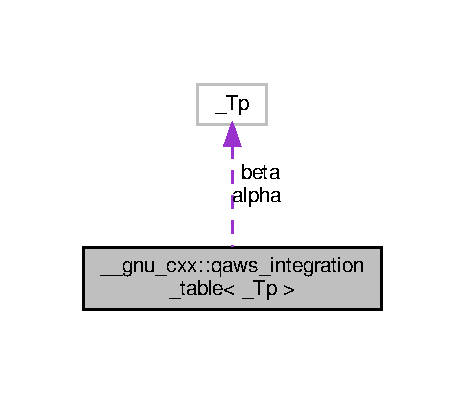
\includegraphics[width=223pt]{struct____gnu__cxx_1_1qaws__integration__table__coll__graph}
\end{center}
\end{figure}
\subsection*{Public Member Functions}
\begin{DoxyCompactItemize}
\item 
\hyperlink{struct____gnu__cxx_1_1qaws__integration__table_a2fc28f96d3219257c427f50bb6928510}{qaws\+\_\+integration\+\_\+table} (\hyperlink{namespace____gnu__cxx_a3b19a9c800ca194374ef9172290f7d79}{\+\_\+\+Tp} \+\_\+\+\_\+alpha, \hyperlink{namespace____gnu__cxx_a3b19a9c800ca194374ef9172290f7d79}{\+\_\+\+Tp} \+\_\+\+\_\+beta, int \+\_\+\+\_\+mu, int \+\_\+\+\_\+nu)
\item 
void \hyperlink{struct____gnu__cxx_1_1qaws__integration__table_a72d9ce0c313049e00eb9aaf4502161ea}{initialise} ()
\item 
void \hyperlink{struct____gnu__cxx_1_1qaws__integration__table_af94e459877f7602f68ea80d294927f1e}{set} (\hyperlink{namespace____gnu__cxx_a3b19a9c800ca194374ef9172290f7d79}{\+\_\+\+Tp} \+\_\+\+\_\+alpha, \hyperlink{namespace____gnu__cxx_a3b19a9c800ca194374ef9172290f7d79}{\+\_\+\+Tp} \+\_\+\+\_\+beta, int \+\_\+\+\_\+mu, int \+\_\+\+\_\+nu)
\end{DoxyCompactItemize}
\subsection*{Public Attributes}
\begin{DoxyCompactItemize}
\item 
\hyperlink{namespace____gnu__cxx_a3b19a9c800ca194374ef9172290f7d79}{\+\_\+\+Tp} \hyperlink{struct____gnu__cxx_1_1qaws__integration__table_a22b7131c633fe090ec1055d51b486bc0}{alpha}
\item 
\hyperlink{namespace____gnu__cxx_a3b19a9c800ca194374ef9172290f7d79}{\+\_\+\+Tp} \hyperlink{struct____gnu__cxx_1_1qaws__integration__table_ad7cdd51af800d8830907d0718035753c}{beta}
\item 
int \hyperlink{struct____gnu__cxx_1_1qaws__integration__table_a27e7db2fb032dc33759509c9c55546dc}{mu}
\item 
int \hyperlink{struct____gnu__cxx_1_1qaws__integration__table_acc78257f8dffad045fe66a13b9c7c434}{nu}
\item 
std\+::array$<$ \hyperlink{namespace____gnu__cxx_a3b19a9c800ca194374ef9172290f7d79}{\+\_\+\+Tp}, 25 $>$ \hyperlink{struct____gnu__cxx_1_1qaws__integration__table_a6549e81e45d5c4196301c945f707f221}{rg}
\item 
std\+::array$<$ \hyperlink{namespace____gnu__cxx_a3b19a9c800ca194374ef9172290f7d79}{\+\_\+\+Tp}, 25 $>$ \hyperlink{struct____gnu__cxx_1_1qaws__integration__table_a7b954bd038be5e62ade0abf9283e90af}{rh}
\item 
std\+::array$<$ \hyperlink{namespace____gnu__cxx_a3b19a9c800ca194374ef9172290f7d79}{\+\_\+\+Tp}, 25 $>$ \hyperlink{struct____gnu__cxx_1_1qaws__integration__table_aa38340ca8677164ecd511a35d5d2a8e7}{ri}
\item 
std\+::array$<$ \hyperlink{namespace____gnu__cxx_a3b19a9c800ca194374ef9172290f7d79}{\+\_\+\+Tp}, 25 $>$ \hyperlink{struct____gnu__cxx_1_1qaws__integration__table_a1b6aa4c79cb8c470510cabc5a502327c}{rj}
\end{DoxyCompactItemize}


\subsection{Detailed Description}
\subsubsection*{template$<$typename \+\_\+\+Tp$>$\newline
struct \+\_\+\+\_\+gnu\+\_\+cxx\+::qaws\+\_\+integration\+\_\+table$<$ \+\_\+\+Tp $>$}

This structure manages integration of functions with optional singular factors \[ log(x - \alpha) log(\beta - x) \] 

Definition at line 37 of file qaws\+\_\+integration\+\_\+table.\+h.



\subsection{Constructor \& Destructor Documentation}
\mbox{\Hypertarget{struct____gnu__cxx_1_1qaws__integration__table_a2fc28f96d3219257c427f50bb6928510}\label{struct____gnu__cxx_1_1qaws__integration__table_a2fc28f96d3219257c427f50bb6928510}} 
\index{\+\_\+\+\_\+gnu\+\_\+cxx\+::qaws\+\_\+integration\+\_\+table@{\+\_\+\+\_\+gnu\+\_\+cxx\+::qaws\+\_\+integration\+\_\+table}!qaws\+\_\+integration\+\_\+table@{qaws\+\_\+integration\+\_\+table}}
\index{qaws\+\_\+integration\+\_\+table@{qaws\+\_\+integration\+\_\+table}!\+\_\+\+\_\+gnu\+\_\+cxx\+::qaws\+\_\+integration\+\_\+table@{\+\_\+\+\_\+gnu\+\_\+cxx\+::qaws\+\_\+integration\+\_\+table}}
\subsubsection{\texorpdfstring{qaws\+\_\+integration\+\_\+table()}{qaws\_integration\_table()}}
{\footnotesize\ttfamily template$<$typename \+\_\+\+Tp $>$ \\
\hyperlink{struct____gnu__cxx_1_1qaws__integration__table}{\+\_\+\+\_\+gnu\+\_\+cxx\+::qaws\+\_\+integration\+\_\+table}$<$ \hyperlink{namespace____gnu__cxx_a3b19a9c800ca194374ef9172290f7d79}{\+\_\+\+Tp} $>$\+::\hyperlink{struct____gnu__cxx_1_1qaws__integration__table}{qaws\+\_\+integration\+\_\+table} (\begin{DoxyParamCaption}\item[{\hyperlink{namespace____gnu__cxx_a3b19a9c800ca194374ef9172290f7d79}{\+\_\+\+Tp}}]{\+\_\+\+\_\+alpha,  }\item[{\hyperlink{namespace____gnu__cxx_a3b19a9c800ca194374ef9172290f7d79}{\+\_\+\+Tp}}]{\+\_\+\+\_\+beta,  }\item[{int}]{\+\_\+\+\_\+mu,  }\item[{int}]{\+\_\+\+\_\+nu }\end{DoxyParamCaption})}



Definition at line 29 of file qaws\+\_\+integration\+\_\+table.\+tcc.



References \+\_\+\+\_\+gnu\+\_\+cxx\+::\+\_\+\+Tp, \+\_\+\+\_\+gnu\+\_\+cxx\+::qaws\+\_\+integration\+\_\+table$<$ \+\_\+\+Tp $>$\+::alpha, \+\_\+\+\_\+gnu\+\_\+cxx\+::qaws\+\_\+integration\+\_\+table$<$ \+\_\+\+Tp $>$\+::beta, \+\_\+\+\_\+gnu\+\_\+cxx\+::qaws\+\_\+integration\+\_\+table$<$ \+\_\+\+Tp $>$\+::initialise(), \+\_\+\+\_\+gnu\+\_\+cxx\+::qaws\+\_\+integration\+\_\+table$<$ \+\_\+\+Tp $>$\+::mu, and \+\_\+\+\_\+gnu\+\_\+cxx\+::qaws\+\_\+integration\+\_\+table$<$ \+\_\+\+Tp $>$\+::nu.


\begin{DoxyCode}
31     : \hyperlink{struct____gnu__cxx_1_1qaws__integration__table_a22b7131c633fe090ec1055d51b486bc0}{alpha}(\_\_alpha),
32       \hyperlink{struct____gnu__cxx_1_1qaws__integration__table_ad7cdd51af800d8830907d0718035753c}{beta}(\_\_beta),
33       \hyperlink{struct____gnu__cxx_1_1qaws__integration__table_a27e7db2fb032dc33759509c9c55546dc}{mu}(\_\_mu),
34       \hyperlink{struct____gnu__cxx_1_1qaws__integration__table_acc78257f8dffad045fe66a13b9c7c434}{nu}(\_\_nu)
35     \{
36       \textcolor{keywordflow}{if} (this->\hyperlink{struct____gnu__cxx_1_1qaws__integration__table_a22b7131c633fe090ec1055d51b486bc0}{alpha} < \hyperlink{namespace____gnu__cxx_a3b19a9c800ca194374ef9172290f7d79}{\_Tp}\{-1\})
37         std::\_\_throw\_domain\_error(\textcolor{stringliteral}{"qaws\_integration\_table: "}
38                                   \textcolor{stringliteral}{"alalpha must be greater than -1.0"});
39       \textcolor{keywordflow}{if} (this->\hyperlink{struct____gnu__cxx_1_1qaws__integration__table_ad7cdd51af800d8830907d0718035753c}{beta} < \hyperlink{namespace____gnu__cxx_a3b19a9c800ca194374ef9172290f7d79}{\_Tp}\{-1\})
40         std::\_\_throw\_domain\_error(\textcolor{stringliteral}{"qaws\_integration\_table: "}
41                                   \textcolor{stringliteral}{"albeta must be greater than -1.0"});
42       \textcolor{keywordflow}{if} (this->\hyperlink{struct____gnu__cxx_1_1qaws__integration__table_a27e7db2fb032dc33759509c9c55546dc}{mu} != 0 && this->\hyperlink{struct____gnu__cxx_1_1qaws__integration__table_a27e7db2fb032dc33759509c9c55546dc}{mu} != 1)
43         std::\_\_throw\_domain\_error(\textcolor{stringliteral}{"qaws\_integration\_table: "}
44                                   \textcolor{stringliteral}{"almu must be 0 or 1"});
45       \textcolor{keywordflow}{if} (this->\hyperlink{struct____gnu__cxx_1_1qaws__integration__table_acc78257f8dffad045fe66a13b9c7c434}{nu} != 0 && this->\hyperlink{struct____gnu__cxx_1_1qaws__integration__table_acc78257f8dffad045fe66a13b9c7c434}{nu} != 1)
46         std::\_\_throw\_domain\_error(\textcolor{stringliteral}{"qaws\_integration\_table: "}
47                                   \textcolor{stringliteral}{"alnu must be 0 or 1"});
48 
49       this->\hyperlink{struct____gnu__cxx_1_1qaws__integration__table_a72d9ce0c313049e00eb9aaf4502161ea}{initialise}();
50     \}
\end{DoxyCode}


\subsection{Member Function Documentation}
\mbox{\Hypertarget{struct____gnu__cxx_1_1qaws__integration__table_a72d9ce0c313049e00eb9aaf4502161ea}\label{struct____gnu__cxx_1_1qaws__integration__table_a72d9ce0c313049e00eb9aaf4502161ea}} 
\index{\+\_\+\+\_\+gnu\+\_\+cxx\+::qaws\+\_\+integration\+\_\+table@{\+\_\+\+\_\+gnu\+\_\+cxx\+::qaws\+\_\+integration\+\_\+table}!initialise@{initialise}}
\index{initialise@{initialise}!\+\_\+\+\_\+gnu\+\_\+cxx\+::qaws\+\_\+integration\+\_\+table@{\+\_\+\+\_\+gnu\+\_\+cxx\+::qaws\+\_\+integration\+\_\+table}}
\subsubsection{\texorpdfstring{initialise()}{initialise()}}
{\footnotesize\ttfamily template$<$typename \+\_\+\+Tp $>$ \\
void \hyperlink{struct____gnu__cxx_1_1qaws__integration__table}{\+\_\+\+\_\+gnu\+\_\+cxx\+::qaws\+\_\+integration\+\_\+table}$<$ \hyperlink{namespace____gnu__cxx_a3b19a9c800ca194374ef9172290f7d79}{\+\_\+\+Tp} $>$\+::initialise (\begin{DoxyParamCaption}{ }\end{DoxyParamCaption})}



Definition at line 80 of file qaws\+\_\+integration\+\_\+table.\+tcc.



References \+\_\+\+\_\+gnu\+\_\+cxx\+::\+\_\+\+Tp, \+\_\+\+\_\+gnu\+\_\+cxx\+::qaws\+\_\+integration\+\_\+table$<$ \+\_\+\+Tp $>$\+::alpha, \+\_\+\+\_\+gnu\+\_\+cxx\+::qaws\+\_\+integration\+\_\+table$<$ \+\_\+\+Tp $>$\+::beta, \+\_\+\+\_\+gnu\+\_\+cxx\+::qaws\+\_\+integration\+\_\+table$<$ \+\_\+\+Tp $>$\+::rg, \+\_\+\+\_\+gnu\+\_\+cxx\+::qaws\+\_\+integration\+\_\+table$<$ \+\_\+\+Tp $>$\+::rh, \+\_\+\+\_\+gnu\+\_\+cxx\+::qaws\+\_\+integration\+\_\+table$<$ \+\_\+\+Tp $>$\+::ri, and \+\_\+\+\_\+gnu\+\_\+cxx\+::qaws\+\_\+integration\+\_\+table$<$ \+\_\+\+Tp $>$\+::rj.



Referenced by \+\_\+\+\_\+gnu\+\_\+cxx\+::qaws\+\_\+integration\+\_\+table$<$ \+\_\+\+Tp $>$\+::qaws\+\_\+integration\+\_\+table(), and \+\_\+\+\_\+gnu\+\_\+cxx\+::qaws\+\_\+integration\+\_\+table$<$ \+\_\+\+Tp $>$\+::set().


\begin{DoxyCode}
81     \{
82       \textcolor{keyword}{const} \textcolor{keyword}{auto} \_\_alpha\_p1 = this->\hyperlink{struct____gnu__cxx_1_1qaws__integration__table_a22b7131c633fe090ec1055d51b486bc0}{alpha} + \hyperlink{namespace____gnu__cxx_a3b19a9c800ca194374ef9172290f7d79}{\_Tp}\{1\};
83       \textcolor{keyword}{const} \textcolor{keyword}{auto} \_\_beta\_p1 = this->\hyperlink{struct____gnu__cxx_1_1qaws__integration__table_ad7cdd51af800d8830907d0718035753c}{beta} + \hyperlink{namespace____gnu__cxx_a3b19a9c800ca194374ef9172290f7d79}{\_Tp}\{1\};
84 
85       \textcolor{keyword}{const} \textcolor{keyword}{auto} \_\_alpha\_p2 = this->\hyperlink{struct____gnu__cxx_1_1qaws__integration__table_a22b7131c633fe090ec1055d51b486bc0}{alpha} + \hyperlink{namespace____gnu__cxx_a3b19a9c800ca194374ef9172290f7d79}{\_Tp}\{2\};
86       \textcolor{keyword}{const} \textcolor{keyword}{auto} \_\_beta\_p2 = this->\hyperlink{struct____gnu__cxx_1_1qaws__integration__table_ad7cdd51af800d8830907d0718035753c}{beta} + \hyperlink{namespace____gnu__cxx_a3b19a9c800ca194374ef9172290f7d79}{\_Tp}\{2\};
87 
88       \textcolor{keyword}{const} \textcolor{keyword}{auto} \_\_r\_alpha = std::pow(\hyperlink{namespace____gnu__cxx_a3b19a9c800ca194374ef9172290f7d79}{\_Tp}\{2\}, \_\_alpha\_p1);
89       \textcolor{keyword}{const} \textcolor{keyword}{auto} \_\_r\_beta = std::pow(\hyperlink{namespace____gnu__cxx_a3b19a9c800ca194374ef9172290f7d79}{\_Tp}\{2\}, \_\_beta\_p1);
90 
91       this->\hyperlink{struct____gnu__cxx_1_1qaws__integration__table_aa38340ca8677164ecd511a35d5d2a8e7}{ri}[0] = \_\_r\_alpha / \_\_alpha\_p1;
92       this->ri[1] = this->ri[0] * this->\hyperlink{struct____gnu__cxx_1_1qaws__integration__table_a22b7131c633fe090ec1055d51b486bc0}{alpha} / \_\_alpha\_p2;
93       \textcolor{keyword}{auto} \_\_an = \hyperlink{namespace____gnu__cxx_a3b19a9c800ca194374ef9172290f7d79}{\_Tp}\{2\};
94       \textcolor{keyword}{auto} \_\_anm1 = \hyperlink{namespace____gnu__cxx_a3b19a9c800ca194374ef9172290f7d79}{\_Tp}\{1\};
95       \textcolor{keywordflow}{for} (\textcolor{keywordtype}{size\_t} \_\_i = 2; \_\_i < this->ri.size(); ++\_\_i)
96         \{
97           this->ri[\_\_i] = -(\_\_r\_alpha
98                           + \_\_an * (\_\_an - \_\_alpha\_p2) * this->ri[\_\_i - 1])
99                         / (\_\_anm1 * (\_\_an + \_\_alpha\_p1));
100           \_\_anm1 = \_\_an;
101           \_\_an += \hyperlink{namespace____gnu__cxx_a3b19a9c800ca194374ef9172290f7d79}{\_Tp}\{1\};
102         \}
103 
104       this->\hyperlink{struct____gnu__cxx_1_1qaws__integration__table_a1b6aa4c79cb8c470510cabc5a502327c}{rj}[0] = \_\_r\_beta / \_\_beta\_p1;
105       this->\hyperlink{struct____gnu__cxx_1_1qaws__integration__table_a1b6aa4c79cb8c470510cabc5a502327c}{rj}[1] = this->\hyperlink{struct____gnu__cxx_1_1qaws__integration__table_a1b6aa4c79cb8c470510cabc5a502327c}{rj}[0] * this->\hyperlink{struct____gnu__cxx_1_1qaws__integration__table_ad7cdd51af800d8830907d0718035753c}{beta} / \_\_beta\_p2;
106       \_\_an = \hyperlink{namespace____gnu__cxx_a3b19a9c800ca194374ef9172290f7d79}{\_Tp}\{2\};
107       \_\_anm1 = \hyperlink{namespace____gnu__cxx_a3b19a9c800ca194374ef9172290f7d79}{\_Tp}\{1\};
108       \textcolor{keywordflow}{for} (\textcolor{keywordtype}{size\_t} \_\_i = 2; \_\_i < this->\hyperlink{struct____gnu__cxx_1_1qaws__integration__table_a1b6aa4c79cb8c470510cabc5a502327c}{rj}.size(); ++\_\_i)
109         \{
110           this->\hyperlink{struct____gnu__cxx_1_1qaws__integration__table_a1b6aa4c79cb8c470510cabc5a502327c}{rj}[\_\_i] = -(\_\_r\_beta
111                           + \_\_an * (\_\_an - \_\_beta\_p2) * this->\hyperlink{struct____gnu__cxx_1_1qaws__integration__table_a1b6aa4c79cb8c470510cabc5a502327c}{rj}[\_\_i - 1])
112                         / (\_\_anm1 * (\_\_an + \_\_beta\_p1));
113           \_\_anm1 = \_\_an;
114           \_\_an += \hyperlink{namespace____gnu__cxx_a3b19a9c800ca194374ef9172290f7d79}{\_Tp}\{1\};
115         \}
116 
117       this->\hyperlink{struct____gnu__cxx_1_1qaws__integration__table_a6549e81e45d5c4196301c945f707f221}{rg}[0] = -this->ri[0] / \_\_alpha\_p1;
118       this->\hyperlink{struct____gnu__cxx_1_1qaws__integration__table_a6549e81e45d5c4196301c945f707f221}{rg}[1] = -this->\hyperlink{struct____gnu__cxx_1_1qaws__integration__table_a6549e81e45d5c4196301c945f707f221}{rg}[0]
119                   - \hyperlink{namespace____gnu__cxx_a3b19a9c800ca194374ef9172290f7d79}{\_Tp}\{2\} * \_\_r\_alpha / (\_\_alpha\_p2 * \_\_alpha\_p2);
120       \_\_an = \hyperlink{namespace____gnu__cxx_a3b19a9c800ca194374ef9172290f7d79}{\_Tp}\{2\};
121       \_\_anm1 = \hyperlink{namespace____gnu__cxx_a3b19a9c800ca194374ef9172290f7d79}{\_Tp}\{1\};
122       \textcolor{keywordflow}{for} (\textcolor{keywordtype}{size\_t} \_\_i = 2; \_\_i < this->\hyperlink{struct____gnu__cxx_1_1qaws__integration__table_a6549e81e45d5c4196301c945f707f221}{rg}.size(); ++\_\_i)
123         \{
124           this->\hyperlink{struct____gnu__cxx_1_1qaws__integration__table_a6549e81e45d5c4196301c945f707f221}{rg}[\_\_i] = -(\_\_an * (\_\_an - \_\_alpha\_p2) * this->\hyperlink{struct____gnu__cxx_1_1qaws__integration__table_a6549e81e45d5c4196301c945f707f221}{rg}[\_\_i - 1]
125                                 - \_\_an * this->ri[\_\_i - 1]
126                                 + \_\_anm1 * this->ri[\_\_i])
127                         / (\_\_anm1 * (\_\_an + \_\_alpha\_p1));
128           \_\_anm1 = \_\_an;
129           \_\_an += \hyperlink{namespace____gnu__cxx_a3b19a9c800ca194374ef9172290f7d79}{\_Tp}\{1\};
130         \}
131 
132       this->\hyperlink{struct____gnu__cxx_1_1qaws__integration__table_a7b954bd038be5e62ade0abf9283e90af}{rh}[0] = -this->\hyperlink{struct____gnu__cxx_1_1qaws__integration__table_a1b6aa4c79cb8c470510cabc5a502327c}{rj}[0] / \_\_beta\_p1;
133       this->\hyperlink{struct____gnu__cxx_1_1qaws__integration__table_a7b954bd038be5e62ade0abf9283e90af}{rh}[1] = -this->\hyperlink{struct____gnu__cxx_1_1qaws__integration__table_a7b954bd038be5e62ade0abf9283e90af}{rh}[0] - \hyperlink{namespace____gnu__cxx_a3b19a9c800ca194374ef9172290f7d79}{\_Tp}\{2\} * \_\_r\_beta / (\_\_beta\_p2 * \_\_beta\_p2);
134       \_\_an = \hyperlink{namespace____gnu__cxx_a3b19a9c800ca194374ef9172290f7d79}{\_Tp}\{2\};
135       \_\_anm1 = \hyperlink{namespace____gnu__cxx_a3b19a9c800ca194374ef9172290f7d79}{\_Tp}\{1\};
136       \textcolor{keywordflow}{for} (\textcolor{keywordtype}{size\_t} \_\_i = 2; \_\_i < this->\hyperlink{struct____gnu__cxx_1_1qaws__integration__table_a7b954bd038be5e62ade0abf9283e90af}{rh}.size(); ++\_\_i)
137         \{
138           this->\hyperlink{struct____gnu__cxx_1_1qaws__integration__table_a7b954bd038be5e62ade0abf9283e90af}{rh}[\_\_i] = -(\_\_an * (\_\_an - \_\_beta\_p2) * this->\hyperlink{struct____gnu__cxx_1_1qaws__integration__table_a7b954bd038be5e62ade0abf9283e90af}{rh}[\_\_i - 1]
139                                 - \_\_an * this->\hyperlink{struct____gnu__cxx_1_1qaws__integration__table_a1b6aa4c79cb8c470510cabc5a502327c}{rj}[\_\_i - 1]
140                                 + \_\_anm1 * this->\hyperlink{struct____gnu__cxx_1_1qaws__integration__table_a1b6aa4c79cb8c470510cabc5a502327c}{rj}[\_\_i])
141                         / (\_\_anm1 * (\_\_an + \_\_beta\_p1));
142           \_\_anm1 = \_\_an;
143           \_\_an += \hyperlink{namespace____gnu__cxx_a3b19a9c800ca194374ef9172290f7d79}{\_Tp}\{1\};
144         \}
145 
146       \textcolor{keywordflow}{for} (\textcolor{keywordtype}{size\_t} \_\_i = 1; \_\_i < this->\hyperlink{struct____gnu__cxx_1_1qaws__integration__table_a1b6aa4c79cb8c470510cabc5a502327c}{rj}.size(); \_\_i += 2)
147         this->\hyperlink{struct____gnu__cxx_1_1qaws__integration__table_a1b6aa4c79cb8c470510cabc5a502327c}{rj}[\_\_i] *= \hyperlink{namespace____gnu__cxx_a3b19a9c800ca194374ef9172290f7d79}{\_Tp}\{-1\};
148       \textcolor{keywordflow}{for} (\textcolor{keywordtype}{size\_t} \_\_i = 1; \_\_i < this->\hyperlink{struct____gnu__cxx_1_1qaws__integration__table_a7b954bd038be5e62ade0abf9283e90af}{rh}.size(); \_\_i += 2)
149         this->\hyperlink{struct____gnu__cxx_1_1qaws__integration__table_a7b954bd038be5e62ade0abf9283e90af}{rh}[\_\_i] *= \hyperlink{namespace____gnu__cxx_a3b19a9c800ca194374ef9172290f7d79}{\_Tp}\{-1\};
150     \}
\end{DoxyCode}
\mbox{\Hypertarget{struct____gnu__cxx_1_1qaws__integration__table_af94e459877f7602f68ea80d294927f1e}\label{struct____gnu__cxx_1_1qaws__integration__table_af94e459877f7602f68ea80d294927f1e}} 
\index{\+\_\+\+\_\+gnu\+\_\+cxx\+::qaws\+\_\+integration\+\_\+table@{\+\_\+\+\_\+gnu\+\_\+cxx\+::qaws\+\_\+integration\+\_\+table}!set@{set}}
\index{set@{set}!\+\_\+\+\_\+gnu\+\_\+cxx\+::qaws\+\_\+integration\+\_\+table@{\+\_\+\+\_\+gnu\+\_\+cxx\+::qaws\+\_\+integration\+\_\+table}}
\subsubsection{\texorpdfstring{set()}{set()}}
{\footnotesize\ttfamily template$<$typename \+\_\+\+Tp $>$ \\
void \hyperlink{struct____gnu__cxx_1_1qaws__integration__table}{\+\_\+\+\_\+gnu\+\_\+cxx\+::qaws\+\_\+integration\+\_\+table}$<$ \hyperlink{namespace____gnu__cxx_a3b19a9c800ca194374ef9172290f7d79}{\+\_\+\+Tp} $>$\+::set (\begin{DoxyParamCaption}\item[{\hyperlink{namespace____gnu__cxx_a3b19a9c800ca194374ef9172290f7d79}{\+\_\+\+Tp}}]{\+\_\+\+\_\+alpha,  }\item[{\hyperlink{namespace____gnu__cxx_a3b19a9c800ca194374ef9172290f7d79}{\+\_\+\+Tp}}]{\+\_\+\+\_\+beta,  }\item[{int}]{\+\_\+\+\_\+mu,  }\item[{int}]{\+\_\+\+\_\+nu }\end{DoxyParamCaption})}



Definition at line 54 of file qaws\+\_\+integration\+\_\+table.\+tcc.



References \+\_\+\+\_\+gnu\+\_\+cxx\+::\+\_\+\+Tp, \+\_\+\+\_\+gnu\+\_\+cxx\+::qaws\+\_\+integration\+\_\+table$<$ \+\_\+\+Tp $>$\+::alpha, \+\_\+\+\_\+gnu\+\_\+cxx\+::qaws\+\_\+integration\+\_\+table$<$ \+\_\+\+Tp $>$\+::beta, \+\_\+\+\_\+gnu\+\_\+cxx\+::qaws\+\_\+integration\+\_\+table$<$ \+\_\+\+Tp $>$\+::initialise(), \+\_\+\+\_\+gnu\+\_\+cxx\+::qaws\+\_\+integration\+\_\+table$<$ \+\_\+\+Tp $>$\+::mu, and \+\_\+\+\_\+gnu\+\_\+cxx\+::qaws\+\_\+integration\+\_\+table$<$ \+\_\+\+Tp $>$\+::nu.


\begin{DoxyCode}
56     \{
57       \textcolor{keywordflow}{if} (\_\_alpha < \hyperlink{namespace____gnu__cxx_a3b19a9c800ca194374ef9172290f7d79}{\_Tp}\{-1\})
58         std::\_\_throw\_domain\_error(\textcolor{stringliteral}{"qaws\_integration\_table: "}
59                                   \textcolor{stringliteral}{"alpha must be greater than -1.0"});
60       \textcolor{keywordflow}{if} (\_\_beta < \hyperlink{namespace____gnu__cxx_a3b19a9c800ca194374ef9172290f7d79}{\_Tp}\{-1\})
61         std::\_\_throw\_domain\_error(\textcolor{stringliteral}{"qaws\_integration\_table: "}
62                                   \textcolor{stringliteral}{"beta must be greater than -1.0"});
63       \textcolor{keywordflow}{if} (\_\_mu != 0 && \_\_mu != 1)
64         std::\_\_throw\_domain\_error(\textcolor{stringliteral}{"qaws\_integration\_table: "}
65                                   \textcolor{stringliteral}{"mu must be 0 or 1"});
66       \textcolor{keywordflow}{if} (\_\_nu != 0 && \_\_nu != 1)
67         std::\_\_throw\_domain\_error(\textcolor{stringliteral}{"qaws\_integration\_table: "}
68                                   \textcolor{stringliteral}{"nu must be 0 or 1"});
69 
70       this->\hyperlink{struct____gnu__cxx_1_1qaws__integration__table_a22b7131c633fe090ec1055d51b486bc0}{alpha} = \_\_alpha;
71       this->\hyperlink{struct____gnu__cxx_1_1qaws__integration__table_ad7cdd51af800d8830907d0718035753c}{beta} = \_\_beta;
72       this->\hyperlink{struct____gnu__cxx_1_1qaws__integration__table_a27e7db2fb032dc33759509c9c55546dc}{mu} = \_\_mu;
73       this->\hyperlink{struct____gnu__cxx_1_1qaws__integration__table_acc78257f8dffad045fe66a13b9c7c434}{nu} = \_\_nu;
74 
75       this->\hyperlink{struct____gnu__cxx_1_1qaws__integration__table_a72d9ce0c313049e00eb9aaf4502161ea}{initialise}();
76     \}
\end{DoxyCode}


\subsection{Member Data Documentation}
\mbox{\Hypertarget{struct____gnu__cxx_1_1qaws__integration__table_a22b7131c633fe090ec1055d51b486bc0}\label{struct____gnu__cxx_1_1qaws__integration__table_a22b7131c633fe090ec1055d51b486bc0}} 
\index{\+\_\+\+\_\+gnu\+\_\+cxx\+::qaws\+\_\+integration\+\_\+table@{\+\_\+\+\_\+gnu\+\_\+cxx\+::qaws\+\_\+integration\+\_\+table}!alpha@{alpha}}
\index{alpha@{alpha}!\+\_\+\+\_\+gnu\+\_\+cxx\+::qaws\+\_\+integration\+\_\+table@{\+\_\+\+\_\+gnu\+\_\+cxx\+::qaws\+\_\+integration\+\_\+table}}
\subsubsection{\texorpdfstring{alpha}{alpha}}
{\footnotesize\ttfamily template$<$typename \+\_\+\+Tp$>$ \\
\hyperlink{namespace____gnu__cxx_a3b19a9c800ca194374ef9172290f7d79}{\+\_\+\+Tp} \hyperlink{struct____gnu__cxx_1_1qaws__integration__table}{\+\_\+\+\_\+gnu\+\_\+cxx\+::qaws\+\_\+integration\+\_\+table}$<$ \hyperlink{namespace____gnu__cxx_a3b19a9c800ca194374ef9172290f7d79}{\+\_\+\+Tp} $>$\+::alpha}



Definition at line 39 of file qaws\+\_\+integration\+\_\+table.\+h.



Referenced by \+\_\+\+\_\+gnu\+\_\+cxx\+::qaws\+\_\+integration\+\_\+table$<$ \+\_\+\+Tp $>$\+::initialise(), \+\_\+\+\_\+gnu\+\_\+cxx\+::qaws\+\_\+integration\+\_\+table$<$ \+\_\+\+Tp $>$\+::qaws\+\_\+integration\+\_\+table(), \+\_\+\+\_\+gnu\+\_\+cxx\+::qc25s(), and \+\_\+\+\_\+gnu\+\_\+cxx\+::qaws\+\_\+integration\+\_\+table$<$ \+\_\+\+Tp $>$\+::set().

\mbox{\Hypertarget{struct____gnu__cxx_1_1qaws__integration__table_ad7cdd51af800d8830907d0718035753c}\label{struct____gnu__cxx_1_1qaws__integration__table_ad7cdd51af800d8830907d0718035753c}} 
\index{\+\_\+\+\_\+gnu\+\_\+cxx\+::qaws\+\_\+integration\+\_\+table@{\+\_\+\+\_\+gnu\+\_\+cxx\+::qaws\+\_\+integration\+\_\+table}!beta@{beta}}
\index{beta@{beta}!\+\_\+\+\_\+gnu\+\_\+cxx\+::qaws\+\_\+integration\+\_\+table@{\+\_\+\+\_\+gnu\+\_\+cxx\+::qaws\+\_\+integration\+\_\+table}}
\subsubsection{\texorpdfstring{beta}{beta}}
{\footnotesize\ttfamily template$<$typename \+\_\+\+Tp$>$ \\
\hyperlink{namespace____gnu__cxx_a3b19a9c800ca194374ef9172290f7d79}{\+\_\+\+Tp} \hyperlink{struct____gnu__cxx_1_1qaws__integration__table}{\+\_\+\+\_\+gnu\+\_\+cxx\+::qaws\+\_\+integration\+\_\+table}$<$ \hyperlink{namespace____gnu__cxx_a3b19a9c800ca194374ef9172290f7d79}{\+\_\+\+Tp} $>$\+::beta}



Definition at line 40 of file qaws\+\_\+integration\+\_\+table.\+h.



Referenced by \+\_\+\+\_\+gnu\+\_\+cxx\+::qaws\+\_\+integration\+\_\+table$<$ \+\_\+\+Tp $>$\+::initialise(), \+\_\+\+\_\+gnu\+\_\+cxx\+::qaws\+\_\+integration\+\_\+table$<$ \+\_\+\+Tp $>$\+::qaws\+\_\+integration\+\_\+table(), \+\_\+\+\_\+gnu\+\_\+cxx\+::qc25s(), and \+\_\+\+\_\+gnu\+\_\+cxx\+::qaws\+\_\+integration\+\_\+table$<$ \+\_\+\+Tp $>$\+::set().

\mbox{\Hypertarget{struct____gnu__cxx_1_1qaws__integration__table_a27e7db2fb032dc33759509c9c55546dc}\label{struct____gnu__cxx_1_1qaws__integration__table_a27e7db2fb032dc33759509c9c55546dc}} 
\index{\+\_\+\+\_\+gnu\+\_\+cxx\+::qaws\+\_\+integration\+\_\+table@{\+\_\+\+\_\+gnu\+\_\+cxx\+::qaws\+\_\+integration\+\_\+table}!mu@{mu}}
\index{mu@{mu}!\+\_\+\+\_\+gnu\+\_\+cxx\+::qaws\+\_\+integration\+\_\+table@{\+\_\+\+\_\+gnu\+\_\+cxx\+::qaws\+\_\+integration\+\_\+table}}
\subsubsection{\texorpdfstring{mu}{mu}}
{\footnotesize\ttfamily template$<$typename \+\_\+\+Tp$>$ \\
int \hyperlink{struct____gnu__cxx_1_1qaws__integration__table}{\+\_\+\+\_\+gnu\+\_\+cxx\+::qaws\+\_\+integration\+\_\+table}$<$ \hyperlink{namespace____gnu__cxx_a3b19a9c800ca194374ef9172290f7d79}{\+\_\+\+Tp} $>$\+::mu}



Definition at line 41 of file qaws\+\_\+integration\+\_\+table.\+h.



Referenced by \+\_\+\+\_\+gnu\+\_\+cxx\+::qaws\+\_\+integration\+\_\+table$<$ \+\_\+\+Tp $>$\+::qaws\+\_\+integration\+\_\+table(), \+\_\+\+\_\+gnu\+\_\+cxx\+::qc25s(), and \+\_\+\+\_\+gnu\+\_\+cxx\+::qaws\+\_\+integration\+\_\+table$<$ \+\_\+\+Tp $>$\+::set().

\mbox{\Hypertarget{struct____gnu__cxx_1_1qaws__integration__table_acc78257f8dffad045fe66a13b9c7c434}\label{struct____gnu__cxx_1_1qaws__integration__table_acc78257f8dffad045fe66a13b9c7c434}} 
\index{\+\_\+\+\_\+gnu\+\_\+cxx\+::qaws\+\_\+integration\+\_\+table@{\+\_\+\+\_\+gnu\+\_\+cxx\+::qaws\+\_\+integration\+\_\+table}!nu@{nu}}
\index{nu@{nu}!\+\_\+\+\_\+gnu\+\_\+cxx\+::qaws\+\_\+integration\+\_\+table@{\+\_\+\+\_\+gnu\+\_\+cxx\+::qaws\+\_\+integration\+\_\+table}}
\subsubsection{\texorpdfstring{nu}{nu}}
{\footnotesize\ttfamily template$<$typename \+\_\+\+Tp$>$ \\
int \hyperlink{struct____gnu__cxx_1_1qaws__integration__table}{\+\_\+\+\_\+gnu\+\_\+cxx\+::qaws\+\_\+integration\+\_\+table}$<$ \hyperlink{namespace____gnu__cxx_a3b19a9c800ca194374ef9172290f7d79}{\+\_\+\+Tp} $>$\+::nu}



Definition at line 42 of file qaws\+\_\+integration\+\_\+table.\+h.



Referenced by \+\_\+\+\_\+gnu\+\_\+cxx\+::qaws\+\_\+integration\+\_\+table$<$ \+\_\+\+Tp $>$\+::qaws\+\_\+integration\+\_\+table(), \+\_\+\+\_\+gnu\+\_\+cxx\+::qc25s(), and \+\_\+\+\_\+gnu\+\_\+cxx\+::qaws\+\_\+integration\+\_\+table$<$ \+\_\+\+Tp $>$\+::set().

\mbox{\Hypertarget{struct____gnu__cxx_1_1qaws__integration__table_a6549e81e45d5c4196301c945f707f221}\label{struct____gnu__cxx_1_1qaws__integration__table_a6549e81e45d5c4196301c945f707f221}} 
\index{\+\_\+\+\_\+gnu\+\_\+cxx\+::qaws\+\_\+integration\+\_\+table@{\+\_\+\+\_\+gnu\+\_\+cxx\+::qaws\+\_\+integration\+\_\+table}!rg@{rg}}
\index{rg@{rg}!\+\_\+\+\_\+gnu\+\_\+cxx\+::qaws\+\_\+integration\+\_\+table@{\+\_\+\+\_\+gnu\+\_\+cxx\+::qaws\+\_\+integration\+\_\+table}}
\subsubsection{\texorpdfstring{rg}{rg}}
{\footnotesize\ttfamily template$<$typename \+\_\+\+Tp$>$ \\
std\+::array$<$\hyperlink{namespace____gnu__cxx_a3b19a9c800ca194374ef9172290f7d79}{\+\_\+\+Tp}, 25$>$ \hyperlink{struct____gnu__cxx_1_1qaws__integration__table}{\+\_\+\+\_\+gnu\+\_\+cxx\+::qaws\+\_\+integration\+\_\+table}$<$ \hyperlink{namespace____gnu__cxx_a3b19a9c800ca194374ef9172290f7d79}{\+\_\+\+Tp} $>$\+::rg}



Definition at line 45 of file qaws\+\_\+integration\+\_\+table.\+h.



Referenced by \+\_\+\+\_\+gnu\+\_\+cxx\+::qaws\+\_\+integration\+\_\+table$<$ \+\_\+\+Tp $>$\+::initialise(), and \+\_\+\+\_\+gnu\+\_\+cxx\+::qc25s().

\mbox{\Hypertarget{struct____gnu__cxx_1_1qaws__integration__table_a7b954bd038be5e62ade0abf9283e90af}\label{struct____gnu__cxx_1_1qaws__integration__table_a7b954bd038be5e62ade0abf9283e90af}} 
\index{\+\_\+\+\_\+gnu\+\_\+cxx\+::qaws\+\_\+integration\+\_\+table@{\+\_\+\+\_\+gnu\+\_\+cxx\+::qaws\+\_\+integration\+\_\+table}!rh@{rh}}
\index{rh@{rh}!\+\_\+\+\_\+gnu\+\_\+cxx\+::qaws\+\_\+integration\+\_\+table@{\+\_\+\+\_\+gnu\+\_\+cxx\+::qaws\+\_\+integration\+\_\+table}}
\subsubsection{\texorpdfstring{rh}{rh}}
{\footnotesize\ttfamily template$<$typename \+\_\+\+Tp$>$ \\
std\+::array$<$\hyperlink{namespace____gnu__cxx_a3b19a9c800ca194374ef9172290f7d79}{\+\_\+\+Tp}, 25$>$ \hyperlink{struct____gnu__cxx_1_1qaws__integration__table}{\+\_\+\+\_\+gnu\+\_\+cxx\+::qaws\+\_\+integration\+\_\+table}$<$ \hyperlink{namespace____gnu__cxx_a3b19a9c800ca194374ef9172290f7d79}{\+\_\+\+Tp} $>$\+::rh}



Definition at line 46 of file qaws\+\_\+integration\+\_\+table.\+h.



Referenced by \+\_\+\+\_\+gnu\+\_\+cxx\+::qaws\+\_\+integration\+\_\+table$<$ \+\_\+\+Tp $>$\+::initialise(), and \+\_\+\+\_\+gnu\+\_\+cxx\+::qc25s().

\mbox{\Hypertarget{struct____gnu__cxx_1_1qaws__integration__table_aa38340ca8677164ecd511a35d5d2a8e7}\label{struct____gnu__cxx_1_1qaws__integration__table_aa38340ca8677164ecd511a35d5d2a8e7}} 
\index{\+\_\+\+\_\+gnu\+\_\+cxx\+::qaws\+\_\+integration\+\_\+table@{\+\_\+\+\_\+gnu\+\_\+cxx\+::qaws\+\_\+integration\+\_\+table}!ri@{ri}}
\index{ri@{ri}!\+\_\+\+\_\+gnu\+\_\+cxx\+::qaws\+\_\+integration\+\_\+table@{\+\_\+\+\_\+gnu\+\_\+cxx\+::qaws\+\_\+integration\+\_\+table}}
\subsubsection{\texorpdfstring{ri}{ri}}
{\footnotesize\ttfamily template$<$typename \+\_\+\+Tp$>$ \\
std\+::array$<$\hyperlink{namespace____gnu__cxx_a3b19a9c800ca194374ef9172290f7d79}{\+\_\+\+Tp}, 25$>$ \hyperlink{struct____gnu__cxx_1_1qaws__integration__table}{\+\_\+\+\_\+gnu\+\_\+cxx\+::qaws\+\_\+integration\+\_\+table}$<$ \hyperlink{namespace____gnu__cxx_a3b19a9c800ca194374ef9172290f7d79}{\+\_\+\+Tp} $>$\+::ri}



Definition at line 43 of file qaws\+\_\+integration\+\_\+table.\+h.



Referenced by \+\_\+\+\_\+gnu\+\_\+cxx\+::qaws\+\_\+integration\+\_\+table$<$ \+\_\+\+Tp $>$\+::initialise(), and \+\_\+\+\_\+gnu\+\_\+cxx\+::qc25s().

\mbox{\Hypertarget{struct____gnu__cxx_1_1qaws__integration__table_a1b6aa4c79cb8c470510cabc5a502327c}\label{struct____gnu__cxx_1_1qaws__integration__table_a1b6aa4c79cb8c470510cabc5a502327c}} 
\index{\+\_\+\+\_\+gnu\+\_\+cxx\+::qaws\+\_\+integration\+\_\+table@{\+\_\+\+\_\+gnu\+\_\+cxx\+::qaws\+\_\+integration\+\_\+table}!rj@{rj}}
\index{rj@{rj}!\+\_\+\+\_\+gnu\+\_\+cxx\+::qaws\+\_\+integration\+\_\+table@{\+\_\+\+\_\+gnu\+\_\+cxx\+::qaws\+\_\+integration\+\_\+table}}
\subsubsection{\texorpdfstring{rj}{rj}}
{\footnotesize\ttfamily template$<$typename \+\_\+\+Tp$>$ \\
std\+::array$<$\hyperlink{namespace____gnu__cxx_a3b19a9c800ca194374ef9172290f7d79}{\+\_\+\+Tp}, 25$>$ \hyperlink{struct____gnu__cxx_1_1qaws__integration__table}{\+\_\+\+\_\+gnu\+\_\+cxx\+::qaws\+\_\+integration\+\_\+table}$<$ \hyperlink{namespace____gnu__cxx_a3b19a9c800ca194374ef9172290f7d79}{\+\_\+\+Tp} $>$\+::rj}



Definition at line 44 of file qaws\+\_\+integration\+\_\+table.\+h.



Referenced by \+\_\+\+\_\+gnu\+\_\+cxx\+::qaws\+\_\+integration\+\_\+table$<$ \+\_\+\+Tp $>$\+::initialise(), and \+\_\+\+\_\+gnu\+\_\+cxx\+::qc25s().



The documentation for this struct was generated from the following files\+:\begin{DoxyCompactItemize}
\item 
include/ext/\hyperlink{qaws__integration__table_8h}{qaws\+\_\+integration\+\_\+table.\+h}\item 
include/ext/\hyperlink{qaws__integration__table_8tcc}{qaws\+\_\+integration\+\_\+table.\+tcc}\end{DoxyCompactItemize}

\hypertarget{class____gnu__cxx_1_1qk__integrator}{}\section{\+\_\+\+\_\+gnu\+\_\+cxx\+:\+:qk\+\_\+integrator$<$ \+\_\+\+Tp, \+\_\+\+Func\+Tp, \+\_\+\+G\+K\+\_\+rule $>$ Class Template Reference}
\label{class____gnu__cxx_1_1qk__integrator}\index{\+\_\+\+\_\+gnu\+\_\+cxx\+::qk\+\_\+integrator$<$ \+\_\+\+Tp, \+\_\+\+Func\+Tp, \+\_\+\+G\+K\+\_\+rule $>$@{\+\_\+\+\_\+gnu\+\_\+cxx\+::qk\+\_\+integrator$<$ \+\_\+\+Tp, \+\_\+\+Func\+Tp, \+\_\+\+G\+K\+\_\+rule $>$}}


\subsection{Detailed Description}
\subsubsection*{template$<$typename \+\_\+\+Tp, typename \+\_\+\+Func\+Tp, Kronrod\+\_\+\+Rule \+\_\+\+G\+K\+\_\+rule$>$\newline
class \+\_\+\+\_\+gnu\+\_\+cxx\+::qk\+\_\+integrator$<$ \+\_\+\+Tp, \+\_\+\+Func\+Tp, \+\_\+\+G\+K\+\_\+rule $>$}



Definition at line 64 of file gauss\+\_\+kronrod\+\_\+integral.\+tcc.



The documentation for this class was generated from the following file\+:\begin{DoxyCompactItemize}
\item 
include/ext/\hyperlink{gauss__kronrod__integral_8tcc}{gauss\+\_\+kronrod\+\_\+integral.\+tcc}\end{DoxyCompactItemize}

\hypertarget{struct____gnu__cxx_1_1qk__integrator_3_01__Tp_00_01__FuncTp_00_01Kronrod__15_01_4}{}\section{\+\_\+\+\_\+gnu\+\_\+cxx\+:\+:qk\+\_\+integrator$<$ \+\_\+\+Tp, \+\_\+\+Func\+Tp, Kronrod\+\_\+15 $>$ Struct Template Reference}
\label{struct____gnu__cxx_1_1qk__integrator_3_01__Tp_00_01__FuncTp_00_01Kronrod__15_01_4}\index{\+\_\+\+\_\+gnu\+\_\+cxx\+::qk\+\_\+integrator$<$ \+\_\+\+Tp, \+\_\+\+Func\+Tp, Kronrod\+\_\+15 $>$@{\+\_\+\+\_\+gnu\+\_\+cxx\+::qk\+\_\+integrator$<$ \+\_\+\+Tp, \+\_\+\+Func\+Tp, Kronrod\+\_\+15 $>$}}
\subsection*{Static Public Attributes}
\begin{DoxyCompactItemize}
\item 
static constexpr std\+::array$<$ \hyperlink{namespace____gnu__cxx_a3b19a9c800ca194374ef9172290f7d79}{\+\_\+\+Tp}, 4 $>$ \hyperlink{struct____gnu__cxx_1_1qk__integrator_3_01__Tp_00_01__FuncTp_00_01Kronrod__15_01_4_aa127e01fbda9767c7602b5bf6db15bb4}{\+\_\+\+S\+\_\+w\+\_\+gauss}
\item 
static constexpr std\+::array$<$ \hyperlink{namespace____gnu__cxx_a3b19a9c800ca194374ef9172290f7d79}{\+\_\+\+Tp}, 8 $>$ \hyperlink{struct____gnu__cxx_1_1qk__integrator_3_01__Tp_00_01__FuncTp_00_01Kronrod__15_01_4_adc8a907d3714406cbb1cf5df42c26d64}{\+\_\+\+S\+\_\+w\+\_\+kronrod}
\item 
static constexpr std\+::array$<$ \hyperlink{namespace____gnu__cxx_a3b19a9c800ca194374ef9172290f7d79}{\+\_\+\+Tp}, 8 $>$ \hyperlink{struct____gnu__cxx_1_1qk__integrator_3_01__Tp_00_01__FuncTp_00_01Kronrod__15_01_4_a300459f400f0ca243e6817105ab79f27}{\+\_\+\+S\+\_\+x\+\_\+kronrod}
\end{DoxyCompactItemize}


\subsection{Detailed Description}
\subsubsection*{template$<$typename \+\_\+\+Tp, typename \+\_\+\+Func\+Tp$>$\newline
struct \+\_\+\+\_\+gnu\+\_\+cxx\+::qk\+\_\+integrator$<$ \+\_\+\+Tp, \+\_\+\+Func\+Tp, Kronrod\+\_\+15 $>$}

Gauss-\/\+Kronrod 15-\/point rule implementation. 

Definition at line 70 of file gauss\+\_\+kronrod\+\_\+integral.\+tcc.



\subsection{Member Data Documentation}
\mbox{\Hypertarget{struct____gnu__cxx_1_1qk__integrator_3_01__Tp_00_01__FuncTp_00_01Kronrod__15_01_4_aa127e01fbda9767c7602b5bf6db15bb4}\label{struct____gnu__cxx_1_1qk__integrator_3_01__Tp_00_01__FuncTp_00_01Kronrod__15_01_4_aa127e01fbda9767c7602b5bf6db15bb4}} 
\index{\+\_\+\+\_\+gnu\+\_\+cxx\+::qk\+\_\+integrator$<$ \+\_\+\+Tp, \+\_\+\+Func\+Tp, Kronrod\+\_\+15 $>$@{\+\_\+\+\_\+gnu\+\_\+cxx\+::qk\+\_\+integrator$<$ \+\_\+\+Tp, \+\_\+\+Func\+Tp, Kronrod\+\_\+15 $>$}!\+\_\+\+S\+\_\+w\+\_\+gauss@{\+\_\+\+S\+\_\+w\+\_\+gauss}}
\index{\+\_\+\+S\+\_\+w\+\_\+gauss@{\+\_\+\+S\+\_\+w\+\_\+gauss}!\+\_\+\+\_\+gnu\+\_\+cxx\+::qk\+\_\+integrator$<$ \+\_\+\+Tp, \+\_\+\+Func\+Tp, Kronrod\+\_\+15 $>$@{\+\_\+\+\_\+gnu\+\_\+cxx\+::qk\+\_\+integrator$<$ \+\_\+\+Tp, \+\_\+\+Func\+Tp, Kronrod\+\_\+15 $>$}}
\subsubsection{\texorpdfstring{\+\_\+\+S\+\_\+w\+\_\+gauss}{\_S\_w\_gauss}}
{\footnotesize\ttfamily template$<$typename \+\_\+\+Tp , typename \+\_\+\+Func\+Tp $>$ \\
constexpr std\+::array$<$\hyperlink{namespace____gnu__cxx_a3b19a9c800ca194374ef9172290f7d79}{\+\_\+\+Tp}, 4$>$ \hyperlink{class____gnu__cxx_1_1qk__integrator}{\+\_\+\+\_\+gnu\+\_\+cxx\+::qk\+\_\+integrator}$<$ \hyperlink{namespace____gnu__cxx_a3b19a9c800ca194374ef9172290f7d79}{\+\_\+\+Tp}, \+\_\+\+Func\+Tp, Kronrod\+\_\+15 $>$\+::\+\_\+\+S\+\_\+w\+\_\+gauss\hspace{0.3cm}{\ttfamily [static]}}

{\bfseries Initial value\+:}
\begin{DoxyCode}
=
      \{
        \hyperlink{namespace____gnu__cxx_a3b19a9c800ca194374ef9172290f7d79}{\_Tp}\{0.129484966168869693270611432679082L\},
        \hyperlink{namespace____gnu__cxx_a3b19a9c800ca194374ef9172290f7d79}{\_Tp}\{0.279705391489276667901467771423780L\},
        \hyperlink{namespace____gnu__cxx_a3b19a9c800ca194374ef9172290f7d79}{\_Tp}\{0.381830050505118944950369775488975L\},
        \hyperlink{namespace____gnu__cxx_a3b19a9c800ca194374ef9172290f7d79}{\_Tp}\{0.417959183673469387755102040816327L\}
      \}
\end{DoxyCode}


Definition at line 87 of file gauss\+\_\+kronrod\+\_\+integral.\+tcc.

\mbox{\Hypertarget{struct____gnu__cxx_1_1qk__integrator_3_01__Tp_00_01__FuncTp_00_01Kronrod__15_01_4_adc8a907d3714406cbb1cf5df42c26d64}\label{struct____gnu__cxx_1_1qk__integrator_3_01__Tp_00_01__FuncTp_00_01Kronrod__15_01_4_adc8a907d3714406cbb1cf5df42c26d64}} 
\index{\+\_\+\+\_\+gnu\+\_\+cxx\+::qk\+\_\+integrator$<$ \+\_\+\+Tp, \+\_\+\+Func\+Tp, Kronrod\+\_\+15 $>$@{\+\_\+\+\_\+gnu\+\_\+cxx\+::qk\+\_\+integrator$<$ \+\_\+\+Tp, \+\_\+\+Func\+Tp, Kronrod\+\_\+15 $>$}!\+\_\+\+S\+\_\+w\+\_\+kronrod@{\+\_\+\+S\+\_\+w\+\_\+kronrod}}
\index{\+\_\+\+S\+\_\+w\+\_\+kronrod@{\+\_\+\+S\+\_\+w\+\_\+kronrod}!\+\_\+\+\_\+gnu\+\_\+cxx\+::qk\+\_\+integrator$<$ \+\_\+\+Tp, \+\_\+\+Func\+Tp, Kronrod\+\_\+15 $>$@{\+\_\+\+\_\+gnu\+\_\+cxx\+::qk\+\_\+integrator$<$ \+\_\+\+Tp, \+\_\+\+Func\+Tp, Kronrod\+\_\+15 $>$}}
\subsubsection{\texorpdfstring{\+\_\+\+S\+\_\+w\+\_\+kronrod}{\_S\_w\_kronrod}}
{\footnotesize\ttfamily template$<$typename \+\_\+\+Tp , typename \+\_\+\+Func\+Tp $>$ \\
constexpr std\+::array$<$\hyperlink{namespace____gnu__cxx_a3b19a9c800ca194374ef9172290f7d79}{\+\_\+\+Tp}, 8$>$ \hyperlink{class____gnu__cxx_1_1qk__integrator}{\+\_\+\+\_\+gnu\+\_\+cxx\+::qk\+\_\+integrator}$<$ \hyperlink{namespace____gnu__cxx_a3b19a9c800ca194374ef9172290f7d79}{\+\_\+\+Tp}, \+\_\+\+Func\+Tp, Kronrod\+\_\+15 $>$\+::\+\_\+\+S\+\_\+w\+\_\+kronrod\hspace{0.3cm}{\ttfamily [static]}}

{\bfseries Initial value\+:}
\begin{DoxyCode}
=
      \{
        \hyperlink{namespace____gnu__cxx_a3b19a9c800ca194374ef9172290f7d79}{\_Tp}\{0.022935322010529224963732008058970L\},
        \hyperlink{namespace____gnu__cxx_a3b19a9c800ca194374ef9172290f7d79}{\_Tp}\{0.063092092629978553290700663189204L\},
        \hyperlink{namespace____gnu__cxx_a3b19a9c800ca194374ef9172290f7d79}{\_Tp}\{0.104790010322250183839876322541518L\},
        \hyperlink{namespace____gnu__cxx_a3b19a9c800ca194374ef9172290f7d79}{\_Tp}\{0.140653259715525918745189590510238L\},
        \hyperlink{namespace____gnu__cxx_a3b19a9c800ca194374ef9172290f7d79}{\_Tp}\{0.169004726639267902826583426598550L\},
        \hyperlink{namespace____gnu__cxx_a3b19a9c800ca194374ef9172290f7d79}{\_Tp}\{0.190350578064785409913256402421014L\},
        \hyperlink{namespace____gnu__cxx_a3b19a9c800ca194374ef9172290f7d79}{\_Tp}\{0.204432940075298892414161999234649L\},
        \hyperlink{namespace____gnu__cxx_a3b19a9c800ca194374ef9172290f7d79}{\_Tp}\{0.209482141084727828012999174891714L\}
      \}
\end{DoxyCode}


Definition at line 96 of file gauss\+\_\+kronrod\+\_\+integral.\+tcc.

\mbox{\Hypertarget{struct____gnu__cxx_1_1qk__integrator_3_01__Tp_00_01__FuncTp_00_01Kronrod__15_01_4_a300459f400f0ca243e6817105ab79f27}\label{struct____gnu__cxx_1_1qk__integrator_3_01__Tp_00_01__FuncTp_00_01Kronrod__15_01_4_a300459f400f0ca243e6817105ab79f27}} 
\index{\+\_\+\+\_\+gnu\+\_\+cxx\+::qk\+\_\+integrator$<$ \+\_\+\+Tp, \+\_\+\+Func\+Tp, Kronrod\+\_\+15 $>$@{\+\_\+\+\_\+gnu\+\_\+cxx\+::qk\+\_\+integrator$<$ \+\_\+\+Tp, \+\_\+\+Func\+Tp, Kronrod\+\_\+15 $>$}!\+\_\+\+S\+\_\+x\+\_\+kronrod@{\+\_\+\+S\+\_\+x\+\_\+kronrod}}
\index{\+\_\+\+S\+\_\+x\+\_\+kronrod@{\+\_\+\+S\+\_\+x\+\_\+kronrod}!\+\_\+\+\_\+gnu\+\_\+cxx\+::qk\+\_\+integrator$<$ \+\_\+\+Tp, \+\_\+\+Func\+Tp, Kronrod\+\_\+15 $>$@{\+\_\+\+\_\+gnu\+\_\+cxx\+::qk\+\_\+integrator$<$ \+\_\+\+Tp, \+\_\+\+Func\+Tp, Kronrod\+\_\+15 $>$}}
\subsubsection{\texorpdfstring{\+\_\+\+S\+\_\+x\+\_\+kronrod}{\_S\_x\_kronrod}}
{\footnotesize\ttfamily template$<$typename \+\_\+\+Tp , typename \+\_\+\+Func\+Tp $>$ \\
constexpr std\+::array$<$\hyperlink{namespace____gnu__cxx_a3b19a9c800ca194374ef9172290f7d79}{\+\_\+\+Tp}, 8$>$ \hyperlink{class____gnu__cxx_1_1qk__integrator}{\+\_\+\+\_\+gnu\+\_\+cxx\+::qk\+\_\+integrator}$<$ \hyperlink{namespace____gnu__cxx_a3b19a9c800ca194374ef9172290f7d79}{\+\_\+\+Tp}, \+\_\+\+Func\+Tp, Kronrod\+\_\+15 $>$\+::\+\_\+\+S\+\_\+x\+\_\+kronrod\hspace{0.3cm}{\ttfamily [static]}}

{\bfseries Initial value\+:}
\begin{DoxyCode}
=
      \{
        \hyperlink{namespace____gnu__cxx_a3b19a9c800ca194374ef9172290f7d79}{\_Tp}\{0.991455371120812639206854697526329L\},
        \hyperlink{namespace____gnu__cxx_a3b19a9c800ca194374ef9172290f7d79}{\_Tp}\{0.949107912342758524526189684047851L\},
        \hyperlink{namespace____gnu__cxx_a3b19a9c800ca194374ef9172290f7d79}{\_Tp}\{0.864864423359769072789712788640926L\},
        \hyperlink{namespace____gnu__cxx_a3b19a9c800ca194374ef9172290f7d79}{\_Tp}\{0.741531185599394439863864773280788L\},
        \hyperlink{namespace____gnu__cxx_a3b19a9c800ca194374ef9172290f7d79}{\_Tp}\{0.586087235467691130294144838258730L\},
        \hyperlink{namespace____gnu__cxx_a3b19a9c800ca194374ef9172290f7d79}{\_Tp}\{0.405845151377397166906606412076961L\},
        \hyperlink{namespace____gnu__cxx_a3b19a9c800ca194374ef9172290f7d79}{\_Tp}\{0.207784955007898467600689403773245L\},
        \hyperlink{namespace____gnu__cxx_a3b19a9c800ca194374ef9172290f7d79}{\_Tp}\{0.000000000000000000000000000000000L\}
      \}
\end{DoxyCode}


Definition at line 74 of file gauss\+\_\+kronrod\+\_\+integral.\+tcc.



The documentation for this struct was generated from the following file\+:\begin{DoxyCompactItemize}
\item 
include/ext/\hyperlink{gauss__kronrod__integral_8tcc}{gauss\+\_\+kronrod\+\_\+integral.\+tcc}\end{DoxyCompactItemize}

\hypertarget{struct____gnu__cxx_1_1qk__integrator_3_01__Tp_00_01__FuncTp_00_01Kronrod__21_01_4}{}\section{\+\_\+\+\_\+gnu\+\_\+cxx\+:\+:qk\+\_\+integrator$<$ \+\_\+\+Tp, \+\_\+\+Func\+Tp, Kronrod\+\_\+21 $>$ Struct Template Reference}
\label{struct____gnu__cxx_1_1qk__integrator_3_01__Tp_00_01__FuncTp_00_01Kronrod__21_01_4}\index{\+\_\+\+\_\+gnu\+\_\+cxx\+::qk\+\_\+integrator$<$ \+\_\+\+Tp, \+\_\+\+Func\+Tp, Kronrod\+\_\+21 $>$@{\+\_\+\+\_\+gnu\+\_\+cxx\+::qk\+\_\+integrator$<$ \+\_\+\+Tp, \+\_\+\+Func\+Tp, Kronrod\+\_\+21 $>$}}
\subsection*{Static Public Attributes}
\begin{DoxyCompactItemize}
\item 
static constexpr std\+::array$<$ \hyperlink{namespace____gnu__cxx_a3b19a9c800ca194374ef9172290f7d79}{\+\_\+\+Tp}, 5 $>$ \hyperlink{struct____gnu__cxx_1_1qk__integrator_3_01__Tp_00_01__FuncTp_00_01Kronrod__21_01_4_a0d750319ca4a47e5e3c08aaf733959c0}{\+\_\+\+S\+\_\+w\+\_\+gauss}
\item 
static constexpr std\+::array$<$ \hyperlink{namespace____gnu__cxx_a3b19a9c800ca194374ef9172290f7d79}{\+\_\+\+Tp}, 11 $>$ \hyperlink{struct____gnu__cxx_1_1qk__integrator_3_01__Tp_00_01__FuncTp_00_01Kronrod__21_01_4_a1b750580a466d233c9eaecaa4b7694e8}{\+\_\+\+S\+\_\+w\+\_\+kronrod}
\item 
static constexpr std\+::array$<$ \hyperlink{namespace____gnu__cxx_a3b19a9c800ca194374ef9172290f7d79}{\+\_\+\+Tp}, 11 $>$ \hyperlink{struct____gnu__cxx_1_1qk__integrator_3_01__Tp_00_01__FuncTp_00_01Kronrod__21_01_4_a1eb98377a298bd31aa92783c6ec6e51e}{\+\_\+\+S\+\_\+x\+\_\+kronrod}
\end{DoxyCompactItemize}


\subsection{Detailed Description}
\subsubsection*{template$<$typename \+\_\+\+Tp, typename \+\_\+\+Func\+Tp$>$\newline
struct \+\_\+\+\_\+gnu\+\_\+cxx\+::qk\+\_\+integrator$<$ \+\_\+\+Tp, \+\_\+\+Func\+Tp, Kronrod\+\_\+21 $>$}

Gauss-\/\+Kronrod 21-\/point rule implementation. 

Definition at line 113 of file gauss\+\_\+kronrod\+\_\+integral.\+tcc.



\subsection{Member Data Documentation}
\mbox{\Hypertarget{struct____gnu__cxx_1_1qk__integrator_3_01__Tp_00_01__FuncTp_00_01Kronrod__21_01_4_a0d750319ca4a47e5e3c08aaf733959c0}\label{struct____gnu__cxx_1_1qk__integrator_3_01__Tp_00_01__FuncTp_00_01Kronrod__21_01_4_a0d750319ca4a47e5e3c08aaf733959c0}} 
\index{\+\_\+\+\_\+gnu\+\_\+cxx\+::qk\+\_\+integrator$<$ \+\_\+\+Tp, \+\_\+\+Func\+Tp, Kronrod\+\_\+21 $>$@{\+\_\+\+\_\+gnu\+\_\+cxx\+::qk\+\_\+integrator$<$ \+\_\+\+Tp, \+\_\+\+Func\+Tp, Kronrod\+\_\+21 $>$}!\+\_\+\+S\+\_\+w\+\_\+gauss@{\+\_\+\+S\+\_\+w\+\_\+gauss}}
\index{\+\_\+\+S\+\_\+w\+\_\+gauss@{\+\_\+\+S\+\_\+w\+\_\+gauss}!\+\_\+\+\_\+gnu\+\_\+cxx\+::qk\+\_\+integrator$<$ \+\_\+\+Tp, \+\_\+\+Func\+Tp, Kronrod\+\_\+21 $>$@{\+\_\+\+\_\+gnu\+\_\+cxx\+::qk\+\_\+integrator$<$ \+\_\+\+Tp, \+\_\+\+Func\+Tp, Kronrod\+\_\+21 $>$}}
\subsubsection{\texorpdfstring{\+\_\+\+S\+\_\+w\+\_\+gauss}{\_S\_w\_gauss}}
{\footnotesize\ttfamily template$<$typename \+\_\+\+Tp , typename \+\_\+\+Func\+Tp $>$ \\
constexpr std\+::array$<$\hyperlink{namespace____gnu__cxx_a3b19a9c800ca194374ef9172290f7d79}{\+\_\+\+Tp}, 5$>$ \hyperlink{class____gnu__cxx_1_1qk__integrator}{\+\_\+\+\_\+gnu\+\_\+cxx\+::qk\+\_\+integrator}$<$ \hyperlink{namespace____gnu__cxx_a3b19a9c800ca194374ef9172290f7d79}{\+\_\+\+Tp}, \+\_\+\+Func\+Tp, Kronrod\+\_\+21 $>$\+::\+\_\+\+S\+\_\+w\+\_\+gauss\hspace{0.3cm}{\ttfamily [static]}}

{\bfseries Initial value\+:}
\begin{DoxyCode}
=
      \{
        \hyperlink{namespace____gnu__cxx_a3b19a9c800ca194374ef9172290f7d79}{\_Tp}\{0.066671344308688137593568809893332L\},
        \hyperlink{namespace____gnu__cxx_a3b19a9c800ca194374ef9172290f7d79}{\_Tp}\{0.149451349150580593145776339657697L\},
        \hyperlink{namespace____gnu__cxx_a3b19a9c800ca194374ef9172290f7d79}{\_Tp}\{0.219086362515982043995534934228163L\},
        \hyperlink{namespace____gnu__cxx_a3b19a9c800ca194374ef9172290f7d79}{\_Tp}\{0.269266719309996355091226921569469L\},
        \hyperlink{namespace____gnu__cxx_a3b19a9c800ca194374ef9172290f7d79}{\_Tp}\{0.295524224714752870173892994651338L\}
      \}
\end{DoxyCode}


Definition at line 133 of file gauss\+\_\+kronrod\+\_\+integral.\+tcc.

\mbox{\Hypertarget{struct____gnu__cxx_1_1qk__integrator_3_01__Tp_00_01__FuncTp_00_01Kronrod__21_01_4_a1b750580a466d233c9eaecaa4b7694e8}\label{struct____gnu__cxx_1_1qk__integrator_3_01__Tp_00_01__FuncTp_00_01Kronrod__21_01_4_a1b750580a466d233c9eaecaa4b7694e8}} 
\index{\+\_\+\+\_\+gnu\+\_\+cxx\+::qk\+\_\+integrator$<$ \+\_\+\+Tp, \+\_\+\+Func\+Tp, Kronrod\+\_\+21 $>$@{\+\_\+\+\_\+gnu\+\_\+cxx\+::qk\+\_\+integrator$<$ \+\_\+\+Tp, \+\_\+\+Func\+Tp, Kronrod\+\_\+21 $>$}!\+\_\+\+S\+\_\+w\+\_\+kronrod@{\+\_\+\+S\+\_\+w\+\_\+kronrod}}
\index{\+\_\+\+S\+\_\+w\+\_\+kronrod@{\+\_\+\+S\+\_\+w\+\_\+kronrod}!\+\_\+\+\_\+gnu\+\_\+cxx\+::qk\+\_\+integrator$<$ \+\_\+\+Tp, \+\_\+\+Func\+Tp, Kronrod\+\_\+21 $>$@{\+\_\+\+\_\+gnu\+\_\+cxx\+::qk\+\_\+integrator$<$ \+\_\+\+Tp, \+\_\+\+Func\+Tp, Kronrod\+\_\+21 $>$}}
\subsubsection{\texorpdfstring{\+\_\+\+S\+\_\+w\+\_\+kronrod}{\_S\_w\_kronrod}}
{\footnotesize\ttfamily template$<$typename \+\_\+\+Tp , typename \+\_\+\+Func\+Tp $>$ \\
constexpr std\+::array$<$\hyperlink{namespace____gnu__cxx_a3b19a9c800ca194374ef9172290f7d79}{\+\_\+\+Tp}, 11$>$ \hyperlink{class____gnu__cxx_1_1qk__integrator}{\+\_\+\+\_\+gnu\+\_\+cxx\+::qk\+\_\+integrator}$<$ \hyperlink{namespace____gnu__cxx_a3b19a9c800ca194374ef9172290f7d79}{\+\_\+\+Tp}, \+\_\+\+Func\+Tp, Kronrod\+\_\+21 $>$\+::\+\_\+\+S\+\_\+w\+\_\+kronrod\hspace{0.3cm}{\ttfamily [static]}}

{\bfseries Initial value\+:}
\begin{DoxyCode}
=
      \{
        \hyperlink{namespace____gnu__cxx_a3b19a9c800ca194374ef9172290f7d79}{\_Tp}\{0.011694638867371874278064396062192L\},
        \hyperlink{namespace____gnu__cxx_a3b19a9c800ca194374ef9172290f7d79}{\_Tp}\{0.032558162307964727478818972459390L\},
        \hyperlink{namespace____gnu__cxx_a3b19a9c800ca194374ef9172290f7d79}{\_Tp}\{0.054755896574351996031381300244580L\},
        \hyperlink{namespace____gnu__cxx_a3b19a9c800ca194374ef9172290f7d79}{\_Tp}\{0.075039674810919952767043140916190L\},
        \hyperlink{namespace____gnu__cxx_a3b19a9c800ca194374ef9172290f7d79}{\_Tp}\{0.093125454583697605535065465083366L\},
        \hyperlink{namespace____gnu__cxx_a3b19a9c800ca194374ef9172290f7d79}{\_Tp}\{0.109387158802297641899210590325805L\},
        \hyperlink{namespace____gnu__cxx_a3b19a9c800ca194374ef9172290f7d79}{\_Tp}\{0.123491976262065851077958109831074L\},
        \hyperlink{namespace____gnu__cxx_a3b19a9c800ca194374ef9172290f7d79}{\_Tp}\{0.134709217311473325928054001771707L\},
        \hyperlink{namespace____gnu__cxx_a3b19a9c800ca194374ef9172290f7d79}{\_Tp}\{0.142775938577060080797094273138717L\},
        \hyperlink{namespace____gnu__cxx_a3b19a9c800ca194374ef9172290f7d79}{\_Tp}\{0.147739104901338491374841515972068L\},
        \hyperlink{namespace____gnu__cxx_a3b19a9c800ca194374ef9172290f7d79}{\_Tp}\{0.149445554002916905664936468389821L\}
      \}
\end{DoxyCode}


Definition at line 143 of file gauss\+\_\+kronrod\+\_\+integral.\+tcc.

\mbox{\Hypertarget{struct____gnu__cxx_1_1qk__integrator_3_01__Tp_00_01__FuncTp_00_01Kronrod__21_01_4_a1eb98377a298bd31aa92783c6ec6e51e}\label{struct____gnu__cxx_1_1qk__integrator_3_01__Tp_00_01__FuncTp_00_01Kronrod__21_01_4_a1eb98377a298bd31aa92783c6ec6e51e}} 
\index{\+\_\+\+\_\+gnu\+\_\+cxx\+::qk\+\_\+integrator$<$ \+\_\+\+Tp, \+\_\+\+Func\+Tp, Kronrod\+\_\+21 $>$@{\+\_\+\+\_\+gnu\+\_\+cxx\+::qk\+\_\+integrator$<$ \+\_\+\+Tp, \+\_\+\+Func\+Tp, Kronrod\+\_\+21 $>$}!\+\_\+\+S\+\_\+x\+\_\+kronrod@{\+\_\+\+S\+\_\+x\+\_\+kronrod}}
\index{\+\_\+\+S\+\_\+x\+\_\+kronrod@{\+\_\+\+S\+\_\+x\+\_\+kronrod}!\+\_\+\+\_\+gnu\+\_\+cxx\+::qk\+\_\+integrator$<$ \+\_\+\+Tp, \+\_\+\+Func\+Tp, Kronrod\+\_\+21 $>$@{\+\_\+\+\_\+gnu\+\_\+cxx\+::qk\+\_\+integrator$<$ \+\_\+\+Tp, \+\_\+\+Func\+Tp, Kronrod\+\_\+21 $>$}}
\subsubsection{\texorpdfstring{\+\_\+\+S\+\_\+x\+\_\+kronrod}{\_S\_x\_kronrod}}
{\footnotesize\ttfamily template$<$typename \+\_\+\+Tp , typename \+\_\+\+Func\+Tp $>$ \\
constexpr std\+::array$<$\hyperlink{namespace____gnu__cxx_a3b19a9c800ca194374ef9172290f7d79}{\+\_\+\+Tp}, 11$>$ \hyperlink{class____gnu__cxx_1_1qk__integrator}{\+\_\+\+\_\+gnu\+\_\+cxx\+::qk\+\_\+integrator}$<$ \hyperlink{namespace____gnu__cxx_a3b19a9c800ca194374ef9172290f7d79}{\+\_\+\+Tp}, \+\_\+\+Func\+Tp, Kronrod\+\_\+21 $>$\+::\+\_\+\+S\+\_\+x\+\_\+kronrod\hspace{0.3cm}{\ttfamily [static]}}

{\bfseries Initial value\+:}
\begin{DoxyCode}
=
      \{
        \hyperlink{namespace____gnu__cxx_a3b19a9c800ca194374ef9172290f7d79}{\_Tp}\{0.995657163025808080735527280689003L\},
        \hyperlink{namespace____gnu__cxx_a3b19a9c800ca194374ef9172290f7d79}{\_Tp}\{0.973906528517171720077964012084452L\},
        \hyperlink{namespace____gnu__cxx_a3b19a9c800ca194374ef9172290f7d79}{\_Tp}\{0.930157491355708226001207180059508L\},
        \hyperlink{namespace____gnu__cxx_a3b19a9c800ca194374ef9172290f7d79}{\_Tp}\{0.865063366688984510732096688423493L\},
        \hyperlink{namespace____gnu__cxx_a3b19a9c800ca194374ef9172290f7d79}{\_Tp}\{0.780817726586416897063717578345042L\},
        \hyperlink{namespace____gnu__cxx_a3b19a9c800ca194374ef9172290f7d79}{\_Tp}\{0.679409568299024406234327365114874L\},
        \hyperlink{namespace____gnu__cxx_a3b19a9c800ca194374ef9172290f7d79}{\_Tp}\{0.562757134668604683339000099272694L\},
        \hyperlink{namespace____gnu__cxx_a3b19a9c800ca194374ef9172290f7d79}{\_Tp}\{0.433395394129247190799265943165784L\},
        \hyperlink{namespace____gnu__cxx_a3b19a9c800ca194374ef9172290f7d79}{\_Tp}\{0.294392862701460198131126603103866L\},
        \hyperlink{namespace____gnu__cxx_a3b19a9c800ca194374ef9172290f7d79}{\_Tp}\{0.148874338981631210884826001129720L\},
        \hyperlink{namespace____gnu__cxx_a3b19a9c800ca194374ef9172290f7d79}{\_Tp}\{0.000000000000000000000000000000000L\}
      \}
\end{DoxyCode}


Definition at line 117 of file gauss\+\_\+kronrod\+\_\+integral.\+tcc.



The documentation for this struct was generated from the following file\+:\begin{DoxyCompactItemize}
\item 
include/ext/\hyperlink{gauss__kronrod__integral_8tcc}{gauss\+\_\+kronrod\+\_\+integral.\+tcc}\end{DoxyCompactItemize}

\hypertarget{struct____gnu__cxx_1_1qk__integrator_3_01__Tp_00_01__FuncTp_00_01Kronrod__31_01_4}{}\section{\+\_\+\+\_\+gnu\+\_\+cxx\+:\+:qk\+\_\+integrator$<$ \+\_\+\+Tp, \+\_\+\+Func\+Tp, Kronrod\+\_\+31 $>$ Struct Template Reference}
\label{struct____gnu__cxx_1_1qk__integrator_3_01__Tp_00_01__FuncTp_00_01Kronrod__31_01_4}\index{\+\_\+\+\_\+gnu\+\_\+cxx\+::qk\+\_\+integrator$<$ \+\_\+\+Tp, \+\_\+\+Func\+Tp, Kronrod\+\_\+31 $>$@{\+\_\+\+\_\+gnu\+\_\+cxx\+::qk\+\_\+integrator$<$ \+\_\+\+Tp, \+\_\+\+Func\+Tp, Kronrod\+\_\+31 $>$}}
\subsection*{Static Public Attributes}
\begin{DoxyCompactItemize}
\item 
static constexpr std\+::array$<$ \hyperlink{namespace____gnu__cxx_a3b19a9c800ca194374ef9172290f7d79}{\+\_\+\+Tp}, 8 $>$ \hyperlink{struct____gnu__cxx_1_1qk__integrator_3_01__Tp_00_01__FuncTp_00_01Kronrod__31_01_4_a3c8884639349c6d5e61005e36dcdb35b}{\+\_\+\+S\+\_\+w\+\_\+gauss}
\item 
static constexpr std\+::array$<$ \hyperlink{namespace____gnu__cxx_a3b19a9c800ca194374ef9172290f7d79}{\+\_\+\+Tp}, 16 $>$ \hyperlink{struct____gnu__cxx_1_1qk__integrator_3_01__Tp_00_01__FuncTp_00_01Kronrod__31_01_4_a00ea863b8b8adad619408d13428239a8}{\+\_\+\+S\+\_\+w\+\_\+kronrod}
\item 
static constexpr std\+::array$<$ \hyperlink{namespace____gnu__cxx_a3b19a9c800ca194374ef9172290f7d79}{\+\_\+\+Tp}, 16 $>$ \hyperlink{struct____gnu__cxx_1_1qk__integrator_3_01__Tp_00_01__FuncTp_00_01Kronrod__31_01_4_a69f1e7a6d85fcb57cd868436160040ac}{\+\_\+\+S\+\_\+x\+\_\+kronrod}
\end{DoxyCompactItemize}


\subsection{Detailed Description}
\subsubsection*{template$<$typename \+\_\+\+Tp, typename \+\_\+\+Func\+Tp$>$\newline
struct \+\_\+\+\_\+gnu\+\_\+cxx\+::qk\+\_\+integrator$<$ \+\_\+\+Tp, \+\_\+\+Func\+Tp, Kronrod\+\_\+31 $>$}

Gauss-\/\+Kronrod 31-\/point rule implementation. 

Definition at line 163 of file gauss\+\_\+kronrod\+\_\+integral.\+tcc.



\subsection{Member Data Documentation}
\mbox{\Hypertarget{struct____gnu__cxx_1_1qk__integrator_3_01__Tp_00_01__FuncTp_00_01Kronrod__31_01_4_a3c8884639349c6d5e61005e36dcdb35b}\label{struct____gnu__cxx_1_1qk__integrator_3_01__Tp_00_01__FuncTp_00_01Kronrod__31_01_4_a3c8884639349c6d5e61005e36dcdb35b}} 
\index{\+\_\+\+\_\+gnu\+\_\+cxx\+::qk\+\_\+integrator$<$ \+\_\+\+Tp, \+\_\+\+Func\+Tp, Kronrod\+\_\+31 $>$@{\+\_\+\+\_\+gnu\+\_\+cxx\+::qk\+\_\+integrator$<$ \+\_\+\+Tp, \+\_\+\+Func\+Tp, Kronrod\+\_\+31 $>$}!\+\_\+\+S\+\_\+w\+\_\+gauss@{\+\_\+\+S\+\_\+w\+\_\+gauss}}
\index{\+\_\+\+S\+\_\+w\+\_\+gauss@{\+\_\+\+S\+\_\+w\+\_\+gauss}!\+\_\+\+\_\+gnu\+\_\+cxx\+::qk\+\_\+integrator$<$ \+\_\+\+Tp, \+\_\+\+Func\+Tp, Kronrod\+\_\+31 $>$@{\+\_\+\+\_\+gnu\+\_\+cxx\+::qk\+\_\+integrator$<$ \+\_\+\+Tp, \+\_\+\+Func\+Tp, Kronrod\+\_\+31 $>$}}
\subsubsection{\texorpdfstring{\+\_\+\+S\+\_\+w\+\_\+gauss}{\_S\_w\_gauss}}
{\footnotesize\ttfamily template$<$typename \+\_\+\+Tp , typename \+\_\+\+Func\+Tp $>$ \\
constexpr std\+::array$<$\hyperlink{namespace____gnu__cxx_a3b19a9c800ca194374ef9172290f7d79}{\+\_\+\+Tp}, 8$>$ \hyperlink{class____gnu__cxx_1_1qk__integrator}{\+\_\+\+\_\+gnu\+\_\+cxx\+::qk\+\_\+integrator}$<$ \hyperlink{namespace____gnu__cxx_a3b19a9c800ca194374ef9172290f7d79}{\+\_\+\+Tp}, \+\_\+\+Func\+Tp, Kronrod\+\_\+31 $>$\+::\+\_\+\+S\+\_\+w\+\_\+gauss\hspace{0.3cm}{\ttfamily [static]}}

{\bfseries Initial value\+:}
\begin{DoxyCode}
=
      \{
        \hyperlink{namespace____gnu__cxx_a3b19a9c800ca194374ef9172290f7d79}{\_Tp}\{0.030753241996117268354628393577204L\},
        \hyperlink{namespace____gnu__cxx_a3b19a9c800ca194374ef9172290f7d79}{\_Tp}\{0.070366047488108124709267416450667L\},
        \hyperlink{namespace____gnu__cxx_a3b19a9c800ca194374ef9172290f7d79}{\_Tp}\{0.107159220467171935011869546685869L\},
        \hyperlink{namespace____gnu__cxx_a3b19a9c800ca194374ef9172290f7d79}{\_Tp}\{0.139570677926154314447804794511028L\},
        \hyperlink{namespace____gnu__cxx_a3b19a9c800ca194374ef9172290f7d79}{\_Tp}\{0.166269205816993933553200860481209L\},
        \hyperlink{namespace____gnu__cxx_a3b19a9c800ca194374ef9172290f7d79}{\_Tp}\{0.186161000015562211026800561866423L\},
        \hyperlink{namespace____gnu__cxx_a3b19a9c800ca194374ef9172290f7d79}{\_Tp}\{0.198431485327111576456118326443839L\},
        \hyperlink{namespace____gnu__cxx_a3b19a9c800ca194374ef9172290f7d79}{\_Tp}\{0.202578241925561272880620199967519L\}
      \}
\end{DoxyCode}


Definition at line 188 of file gauss\+\_\+kronrod\+\_\+integral.\+tcc.

\mbox{\Hypertarget{struct____gnu__cxx_1_1qk__integrator_3_01__Tp_00_01__FuncTp_00_01Kronrod__31_01_4_a00ea863b8b8adad619408d13428239a8}\label{struct____gnu__cxx_1_1qk__integrator_3_01__Tp_00_01__FuncTp_00_01Kronrod__31_01_4_a00ea863b8b8adad619408d13428239a8}} 
\index{\+\_\+\+\_\+gnu\+\_\+cxx\+::qk\+\_\+integrator$<$ \+\_\+\+Tp, \+\_\+\+Func\+Tp, Kronrod\+\_\+31 $>$@{\+\_\+\+\_\+gnu\+\_\+cxx\+::qk\+\_\+integrator$<$ \+\_\+\+Tp, \+\_\+\+Func\+Tp, Kronrod\+\_\+31 $>$}!\+\_\+\+S\+\_\+w\+\_\+kronrod@{\+\_\+\+S\+\_\+w\+\_\+kronrod}}
\index{\+\_\+\+S\+\_\+w\+\_\+kronrod@{\+\_\+\+S\+\_\+w\+\_\+kronrod}!\+\_\+\+\_\+gnu\+\_\+cxx\+::qk\+\_\+integrator$<$ \+\_\+\+Tp, \+\_\+\+Func\+Tp, Kronrod\+\_\+31 $>$@{\+\_\+\+\_\+gnu\+\_\+cxx\+::qk\+\_\+integrator$<$ \+\_\+\+Tp, \+\_\+\+Func\+Tp, Kronrod\+\_\+31 $>$}}
\subsubsection{\texorpdfstring{\+\_\+\+S\+\_\+w\+\_\+kronrod}{\_S\_w\_kronrod}}
{\footnotesize\ttfamily template$<$typename \+\_\+\+Tp , typename \+\_\+\+Func\+Tp $>$ \\
constexpr std\+::array$<$\hyperlink{namespace____gnu__cxx_a3b19a9c800ca194374ef9172290f7d79}{\+\_\+\+Tp}, 16$>$ \hyperlink{class____gnu__cxx_1_1qk__integrator}{\+\_\+\+\_\+gnu\+\_\+cxx\+::qk\+\_\+integrator}$<$ \hyperlink{namespace____gnu__cxx_a3b19a9c800ca194374ef9172290f7d79}{\+\_\+\+Tp}, \+\_\+\+Func\+Tp, Kronrod\+\_\+31 $>$\+::\+\_\+\+S\+\_\+w\+\_\+kronrod\hspace{0.3cm}{\ttfamily [static]}}

{\bfseries Initial value\+:}
\begin{DoxyCode}
=
      \{
        \hyperlink{namespace____gnu__cxx_a3b19a9c800ca194374ef9172290f7d79}{\_Tp}\{0.005377479872923348987792051430128L\},
        \hyperlink{namespace____gnu__cxx_a3b19a9c800ca194374ef9172290f7d79}{\_Tp}\{0.015007947329316122538374763075807L\},
        \hyperlink{namespace____gnu__cxx_a3b19a9c800ca194374ef9172290f7d79}{\_Tp}\{0.025460847326715320186874001019653L\},
        \hyperlink{namespace____gnu__cxx_a3b19a9c800ca194374ef9172290f7d79}{\_Tp}\{0.035346360791375846222037948478360L\},
        \hyperlink{namespace____gnu__cxx_a3b19a9c800ca194374ef9172290f7d79}{\_Tp}\{0.044589751324764876608227299373280L\},
        \hyperlink{namespace____gnu__cxx_a3b19a9c800ca194374ef9172290f7d79}{\_Tp}\{0.053481524690928087265343147239430L\},
        \hyperlink{namespace____gnu__cxx_a3b19a9c800ca194374ef9172290f7d79}{\_Tp}\{0.062009567800670640285139230960803L\},
        \hyperlink{namespace____gnu__cxx_a3b19a9c800ca194374ef9172290f7d79}{\_Tp}\{0.069854121318728258709520077099147L\},
        \hyperlink{namespace____gnu__cxx_a3b19a9c800ca194374ef9172290f7d79}{\_Tp}\{0.076849680757720378894432777482659L\},
        \hyperlink{namespace____gnu__cxx_a3b19a9c800ca194374ef9172290f7d79}{\_Tp}\{0.083080502823133021038289247286104L\},
        \hyperlink{namespace____gnu__cxx_a3b19a9c800ca194374ef9172290f7d79}{\_Tp}\{0.088564443056211770647275443693774L\},
        \hyperlink{namespace____gnu__cxx_a3b19a9c800ca194374ef9172290f7d79}{\_Tp}\{0.093126598170825321225486872747346L\},
        \hyperlink{namespace____gnu__cxx_a3b19a9c800ca194374ef9172290f7d79}{\_Tp}\{0.096642726983623678505179907627589L\},
        \hyperlink{namespace____gnu__cxx_a3b19a9c800ca194374ef9172290f7d79}{\_Tp}\{0.099173598721791959332393173484603L\},
        \hyperlink{namespace____gnu__cxx_a3b19a9c800ca194374ef9172290f7d79}{\_Tp}\{0.100769845523875595044946662617570L\},
        \hyperlink{namespace____gnu__cxx_a3b19a9c800ca194374ef9172290f7d79}{\_Tp}\{0.101330007014791549017374792767493L\}
      \}
\end{DoxyCode}


Definition at line 201 of file gauss\+\_\+kronrod\+\_\+integral.\+tcc.

\mbox{\Hypertarget{struct____gnu__cxx_1_1qk__integrator_3_01__Tp_00_01__FuncTp_00_01Kronrod__31_01_4_a69f1e7a6d85fcb57cd868436160040ac}\label{struct____gnu__cxx_1_1qk__integrator_3_01__Tp_00_01__FuncTp_00_01Kronrod__31_01_4_a69f1e7a6d85fcb57cd868436160040ac}} 
\index{\+\_\+\+\_\+gnu\+\_\+cxx\+::qk\+\_\+integrator$<$ \+\_\+\+Tp, \+\_\+\+Func\+Tp, Kronrod\+\_\+31 $>$@{\+\_\+\+\_\+gnu\+\_\+cxx\+::qk\+\_\+integrator$<$ \+\_\+\+Tp, \+\_\+\+Func\+Tp, Kronrod\+\_\+31 $>$}!\+\_\+\+S\+\_\+x\+\_\+kronrod@{\+\_\+\+S\+\_\+x\+\_\+kronrod}}
\index{\+\_\+\+S\+\_\+x\+\_\+kronrod@{\+\_\+\+S\+\_\+x\+\_\+kronrod}!\+\_\+\+\_\+gnu\+\_\+cxx\+::qk\+\_\+integrator$<$ \+\_\+\+Tp, \+\_\+\+Func\+Tp, Kronrod\+\_\+31 $>$@{\+\_\+\+\_\+gnu\+\_\+cxx\+::qk\+\_\+integrator$<$ \+\_\+\+Tp, \+\_\+\+Func\+Tp, Kronrod\+\_\+31 $>$}}
\subsubsection{\texorpdfstring{\+\_\+\+S\+\_\+x\+\_\+kronrod}{\_S\_x\_kronrod}}
{\footnotesize\ttfamily template$<$typename \+\_\+\+Tp , typename \+\_\+\+Func\+Tp $>$ \\
constexpr std\+::array$<$\hyperlink{namespace____gnu__cxx_a3b19a9c800ca194374ef9172290f7d79}{\+\_\+\+Tp}, 16$>$ \hyperlink{class____gnu__cxx_1_1qk__integrator}{\+\_\+\+\_\+gnu\+\_\+cxx\+::qk\+\_\+integrator}$<$ \hyperlink{namespace____gnu__cxx_a3b19a9c800ca194374ef9172290f7d79}{\+\_\+\+Tp}, \+\_\+\+Func\+Tp, Kronrod\+\_\+31 $>$\+::\+\_\+\+S\+\_\+x\+\_\+kronrod\hspace{0.3cm}{\ttfamily [static]}}

{\bfseries Initial value\+:}
\begin{DoxyCode}
=
      \{
        \hyperlink{namespace____gnu__cxx_a3b19a9c800ca194374ef9172290f7d79}{\_Tp}\{0.998002298693397060285172840152271L\},
        \hyperlink{namespace____gnu__cxx_a3b19a9c800ca194374ef9172290f7d79}{\_Tp}\{0.987992518020485428489565718586613L\},
        \hyperlink{namespace____gnu__cxx_a3b19a9c800ca194374ef9172290f7d79}{\_Tp}\{0.967739075679139134257347978784337L\},
        \hyperlink{namespace____gnu__cxx_a3b19a9c800ca194374ef9172290f7d79}{\_Tp}\{0.937273392400705904307758947710209L\},
        \hyperlink{namespace____gnu__cxx_a3b19a9c800ca194374ef9172290f7d79}{\_Tp}\{0.897264532344081900882509656454496L\},
        \hyperlink{namespace____gnu__cxx_a3b19a9c800ca194374ef9172290f7d79}{\_Tp}\{0.848206583410427216200648320774217L\},
        \hyperlink{namespace____gnu__cxx_a3b19a9c800ca194374ef9172290f7d79}{\_Tp}\{0.790418501442465932967649294817947L\},
        \hyperlink{namespace____gnu__cxx_a3b19a9c800ca194374ef9172290f7d79}{\_Tp}\{0.724417731360170047416186054613938L\},
        \hyperlink{namespace____gnu__cxx_a3b19a9c800ca194374ef9172290f7d79}{\_Tp}\{0.650996741297416970533735895313275L\},
        \hyperlink{namespace____gnu__cxx_a3b19a9c800ca194374ef9172290f7d79}{\_Tp}\{0.570972172608538847537226737253911L\},
        \hyperlink{namespace____gnu__cxx_a3b19a9c800ca194374ef9172290f7d79}{\_Tp}\{0.485081863640239680693655740232351L\},
        \hyperlink{namespace____gnu__cxx_a3b19a9c800ca194374ef9172290f7d79}{\_Tp}\{0.394151347077563369897207370981045L\},
        \hyperlink{namespace____gnu__cxx_a3b19a9c800ca194374ef9172290f7d79}{\_Tp}\{0.299180007153168812166780024266389L\},
        \hyperlink{namespace____gnu__cxx_a3b19a9c800ca194374ef9172290f7d79}{\_Tp}\{0.201194093997434522300628303394596L\},
        \hyperlink{namespace____gnu__cxx_a3b19a9c800ca194374ef9172290f7d79}{\_Tp}\{0.101142066918717499027074231447392L\},
        \hyperlink{namespace____gnu__cxx_a3b19a9c800ca194374ef9172290f7d79}{\_Tp}\{0.000000000000000000000000000000000L\}
      \}
\end{DoxyCode}


Definition at line 167 of file gauss\+\_\+kronrod\+\_\+integral.\+tcc.



The documentation for this struct was generated from the following file\+:\begin{DoxyCompactItemize}
\item 
include/ext/\hyperlink{gauss__kronrod__integral_8tcc}{gauss\+\_\+kronrod\+\_\+integral.\+tcc}\end{DoxyCompactItemize}

\hypertarget{struct____gnu__cxx_1_1qk__integrator_3_01__Tp_00_01__FuncTp_00_01Kronrod__41_01_4}{}\section{\+\_\+\+\_\+gnu\+\_\+cxx\+:\+:qk\+\_\+integrator$<$ \+\_\+\+Tp, \+\_\+\+Func\+Tp, Kronrod\+\_\+41 $>$ Struct Template Reference}
\label{struct____gnu__cxx_1_1qk__integrator_3_01__Tp_00_01__FuncTp_00_01Kronrod__41_01_4}\index{\+\_\+\+\_\+gnu\+\_\+cxx\+::qk\+\_\+integrator$<$ \+\_\+\+Tp, \+\_\+\+Func\+Tp, Kronrod\+\_\+41 $>$@{\+\_\+\+\_\+gnu\+\_\+cxx\+::qk\+\_\+integrator$<$ \+\_\+\+Tp, \+\_\+\+Func\+Tp, Kronrod\+\_\+41 $>$}}
\subsection*{Static Public Attributes}
\begin{DoxyCompactItemize}
\item 
static constexpr std\+::array$<$ \hyperlink{namespace____gnu__cxx_a3b19a9c800ca194374ef9172290f7d79}{\+\_\+\+Tp}, 10 $>$ \hyperlink{struct____gnu__cxx_1_1qk__integrator_3_01__Tp_00_01__FuncTp_00_01Kronrod__41_01_4_a8fe39fcd7f3d302de90f987b349bc7a6}{\+\_\+\+S\+\_\+w\+\_\+gauss}
\item 
static constexpr std\+::array$<$ \hyperlink{namespace____gnu__cxx_a3b19a9c800ca194374ef9172290f7d79}{\+\_\+\+Tp}, 21 $>$ \hyperlink{struct____gnu__cxx_1_1qk__integrator_3_01__Tp_00_01__FuncTp_00_01Kronrod__41_01_4_a0ca7d785bcc4ea62564da850f4349aa2}{\+\_\+\+S\+\_\+w\+\_\+kronrod}
\item 
static constexpr std\+::array$<$ \hyperlink{namespace____gnu__cxx_a3b19a9c800ca194374ef9172290f7d79}{\+\_\+\+Tp}, 21 $>$ \hyperlink{struct____gnu__cxx_1_1qk__integrator_3_01__Tp_00_01__FuncTp_00_01Kronrod__41_01_4_a0002dac8d27b1ce360e5c2adf88fa916}{\+\_\+\+S\+\_\+x\+\_\+kronrod}
\end{DoxyCompactItemize}


\subsection{Detailed Description}
\subsubsection*{template$<$typename \+\_\+\+Tp, typename \+\_\+\+Func\+Tp$>$\newline
struct \+\_\+\+\_\+gnu\+\_\+cxx\+::qk\+\_\+integrator$<$ \+\_\+\+Tp, \+\_\+\+Func\+Tp, Kronrod\+\_\+41 $>$}

Gauss-\/\+Kronrod 41-\/point rule implementation. 

Definition at line 226 of file gauss\+\_\+kronrod\+\_\+integral.\+tcc.



\subsection{Member Data Documentation}
\mbox{\Hypertarget{struct____gnu__cxx_1_1qk__integrator_3_01__Tp_00_01__FuncTp_00_01Kronrod__41_01_4_a8fe39fcd7f3d302de90f987b349bc7a6}\label{struct____gnu__cxx_1_1qk__integrator_3_01__Tp_00_01__FuncTp_00_01Kronrod__41_01_4_a8fe39fcd7f3d302de90f987b349bc7a6}} 
\index{\+\_\+\+\_\+gnu\+\_\+cxx\+::qk\+\_\+integrator$<$ \+\_\+\+Tp, \+\_\+\+Func\+Tp, Kronrod\+\_\+41 $>$@{\+\_\+\+\_\+gnu\+\_\+cxx\+::qk\+\_\+integrator$<$ \+\_\+\+Tp, \+\_\+\+Func\+Tp, Kronrod\+\_\+41 $>$}!\+\_\+\+S\+\_\+w\+\_\+gauss@{\+\_\+\+S\+\_\+w\+\_\+gauss}}
\index{\+\_\+\+S\+\_\+w\+\_\+gauss@{\+\_\+\+S\+\_\+w\+\_\+gauss}!\+\_\+\+\_\+gnu\+\_\+cxx\+::qk\+\_\+integrator$<$ \+\_\+\+Tp, \+\_\+\+Func\+Tp, Kronrod\+\_\+41 $>$@{\+\_\+\+\_\+gnu\+\_\+cxx\+::qk\+\_\+integrator$<$ \+\_\+\+Tp, \+\_\+\+Func\+Tp, Kronrod\+\_\+41 $>$}}
\subsubsection{\texorpdfstring{\+\_\+\+S\+\_\+w\+\_\+gauss}{\_S\_w\_gauss}}
{\footnotesize\ttfamily template$<$typename \+\_\+\+Tp , typename \+\_\+\+Func\+Tp $>$ \\
constexpr std\+::array$<$\hyperlink{namespace____gnu__cxx_a3b19a9c800ca194374ef9172290f7d79}{\+\_\+\+Tp}, 10$>$ \hyperlink{class____gnu__cxx_1_1qk__integrator}{\+\_\+\+\_\+gnu\+\_\+cxx\+::qk\+\_\+integrator}$<$ \hyperlink{namespace____gnu__cxx_a3b19a9c800ca194374ef9172290f7d79}{\+\_\+\+Tp}, \+\_\+\+Func\+Tp, Kronrod\+\_\+41 $>$\+::\+\_\+\+S\+\_\+w\+\_\+gauss\hspace{0.3cm}{\ttfamily [static]}}

{\bfseries Initial value\+:}
\begin{DoxyCode}
=
      \{
        \hyperlink{namespace____gnu__cxx_a3b19a9c800ca194374ef9172290f7d79}{\_Tp}\{0.017614007139152118311861962351853L\},
        \hyperlink{namespace____gnu__cxx_a3b19a9c800ca194374ef9172290f7d79}{\_Tp}\{0.040601429800386941331039952274932L\},
        \hyperlink{namespace____gnu__cxx_a3b19a9c800ca194374ef9172290f7d79}{\_Tp}\{0.062672048334109063569506535187042L\},
        \hyperlink{namespace____gnu__cxx_a3b19a9c800ca194374ef9172290f7d79}{\_Tp}\{0.083276741576704748724758143222046L\},
        \hyperlink{namespace____gnu__cxx_a3b19a9c800ca194374ef9172290f7d79}{\_Tp}\{0.101930119817240435036750135480350L\},
        \hyperlink{namespace____gnu__cxx_a3b19a9c800ca194374ef9172290f7d79}{\_Tp}\{0.118194531961518417312377377711382L\},
        \hyperlink{namespace____gnu__cxx_a3b19a9c800ca194374ef9172290f7d79}{\_Tp}\{0.131688638449176626898494499748163L\},
        \hyperlink{namespace____gnu__cxx_a3b19a9c800ca194374ef9172290f7d79}{\_Tp}\{0.142096109318382051329298325067165L\},
        \hyperlink{namespace____gnu__cxx_a3b19a9c800ca194374ef9172290f7d79}{\_Tp}\{0.149172986472603746787828737001969L\},
        \hyperlink{namespace____gnu__cxx_a3b19a9c800ca194374ef9172290f7d79}{\_Tp}\{0.152753387130725850698084331955098L\}
      \}
\end{DoxyCode}


Definition at line 256 of file gauss\+\_\+kronrod\+\_\+integral.\+tcc.

\mbox{\Hypertarget{struct____gnu__cxx_1_1qk__integrator_3_01__Tp_00_01__FuncTp_00_01Kronrod__41_01_4_a0ca7d785bcc4ea62564da850f4349aa2}\label{struct____gnu__cxx_1_1qk__integrator_3_01__Tp_00_01__FuncTp_00_01Kronrod__41_01_4_a0ca7d785bcc4ea62564da850f4349aa2}} 
\index{\+\_\+\+\_\+gnu\+\_\+cxx\+::qk\+\_\+integrator$<$ \+\_\+\+Tp, \+\_\+\+Func\+Tp, Kronrod\+\_\+41 $>$@{\+\_\+\+\_\+gnu\+\_\+cxx\+::qk\+\_\+integrator$<$ \+\_\+\+Tp, \+\_\+\+Func\+Tp, Kronrod\+\_\+41 $>$}!\+\_\+\+S\+\_\+w\+\_\+kronrod@{\+\_\+\+S\+\_\+w\+\_\+kronrod}}
\index{\+\_\+\+S\+\_\+w\+\_\+kronrod@{\+\_\+\+S\+\_\+w\+\_\+kronrod}!\+\_\+\+\_\+gnu\+\_\+cxx\+::qk\+\_\+integrator$<$ \+\_\+\+Tp, \+\_\+\+Func\+Tp, Kronrod\+\_\+41 $>$@{\+\_\+\+\_\+gnu\+\_\+cxx\+::qk\+\_\+integrator$<$ \+\_\+\+Tp, \+\_\+\+Func\+Tp, Kronrod\+\_\+41 $>$}}
\subsubsection{\texorpdfstring{\+\_\+\+S\+\_\+w\+\_\+kronrod}{\_S\_w\_kronrod}}
{\footnotesize\ttfamily template$<$typename \+\_\+\+Tp , typename \+\_\+\+Func\+Tp $>$ \\
constexpr std\+::array$<$\hyperlink{namespace____gnu__cxx_a3b19a9c800ca194374ef9172290f7d79}{\+\_\+\+Tp}, 21$>$ \hyperlink{class____gnu__cxx_1_1qk__integrator}{\+\_\+\+\_\+gnu\+\_\+cxx\+::qk\+\_\+integrator}$<$ \hyperlink{namespace____gnu__cxx_a3b19a9c800ca194374ef9172290f7d79}{\+\_\+\+Tp}, \+\_\+\+Func\+Tp, Kronrod\+\_\+41 $>$\+::\+\_\+\+S\+\_\+w\+\_\+kronrod\hspace{0.3cm}{\ttfamily [static]}}

{\bfseries Initial value\+:}
\begin{DoxyCode}
=
      \{
        \hyperlink{namespace____gnu__cxx_a3b19a9c800ca194374ef9172290f7d79}{\_Tp}\{0.003073583718520531501218293246031L\},
        \hyperlink{namespace____gnu__cxx_a3b19a9c800ca194374ef9172290f7d79}{\_Tp}\{0.008600269855642942198661787950102L\},
        \hyperlink{namespace____gnu__cxx_a3b19a9c800ca194374ef9172290f7d79}{\_Tp}\{0.014626169256971252983787960308868L\},
        \hyperlink{namespace____gnu__cxx_a3b19a9c800ca194374ef9172290f7d79}{\_Tp}\{0.020388373461266523598010231432755L\},
        \hyperlink{namespace____gnu__cxx_a3b19a9c800ca194374ef9172290f7d79}{\_Tp}\{0.025882133604951158834505067096153L\},
        \hyperlink{namespace____gnu__cxx_a3b19a9c800ca194374ef9172290f7d79}{\_Tp}\{0.031287306777032798958543119323801L\},
        \hyperlink{namespace____gnu__cxx_a3b19a9c800ca194374ef9172290f7d79}{\_Tp}\{0.036600169758200798030557240707211L\},
        \hyperlink{namespace____gnu__cxx_a3b19a9c800ca194374ef9172290f7d79}{\_Tp}\{0.041668873327973686263788305936895L\},
        \hyperlink{namespace____gnu__cxx_a3b19a9c800ca194374ef9172290f7d79}{\_Tp}\{0.046434821867497674720231880926108L\},
        \hyperlink{namespace____gnu__cxx_a3b19a9c800ca194374ef9172290f7d79}{\_Tp}\{0.050944573923728691932707670050345L\},
        \hyperlink{namespace____gnu__cxx_a3b19a9c800ca194374ef9172290f7d79}{\_Tp}\{0.055195105348285994744832372419777L\},
        \hyperlink{namespace____gnu__cxx_a3b19a9c800ca194374ef9172290f7d79}{\_Tp}\{0.059111400880639572374967220648594L\},
        \hyperlink{namespace____gnu__cxx_a3b19a9c800ca194374ef9172290f7d79}{\_Tp}\{0.062653237554781168025870122174255L\},
        \hyperlink{namespace____gnu__cxx_a3b19a9c800ca194374ef9172290f7d79}{\_Tp}\{0.065834597133618422111563556969398L\},
        \hyperlink{namespace____gnu__cxx_a3b19a9c800ca194374ef9172290f7d79}{\_Tp}\{0.068648672928521619345623411885368L\},
        \hyperlink{namespace____gnu__cxx_a3b19a9c800ca194374ef9172290f7d79}{\_Tp}\{0.071054423553444068305790361723210L\},
        \hyperlink{namespace____gnu__cxx_a3b19a9c800ca194374ef9172290f7d79}{\_Tp}\{0.073030690332786667495189417658913L\},
        \hyperlink{namespace____gnu__cxx_a3b19a9c800ca194374ef9172290f7d79}{\_Tp}\{0.074582875400499188986581418362488L\},
        \hyperlink{namespace____gnu__cxx_a3b19a9c800ca194374ef9172290f7d79}{\_Tp}\{0.075704497684556674659542775376617L\},
        \hyperlink{namespace____gnu__cxx_a3b19a9c800ca194374ef9172290f7d79}{\_Tp}\{0.076377867672080736705502835038061L\},
        \hyperlink{namespace____gnu__cxx_a3b19a9c800ca194374ef9172290f7d79}{\_Tp}\{0.076600711917999656445049901530102L\}
      \}
\end{DoxyCode}


Definition at line 271 of file gauss\+\_\+kronrod\+\_\+integral.\+tcc.

\mbox{\Hypertarget{struct____gnu__cxx_1_1qk__integrator_3_01__Tp_00_01__FuncTp_00_01Kronrod__41_01_4_a0002dac8d27b1ce360e5c2adf88fa916}\label{struct____gnu__cxx_1_1qk__integrator_3_01__Tp_00_01__FuncTp_00_01Kronrod__41_01_4_a0002dac8d27b1ce360e5c2adf88fa916}} 
\index{\+\_\+\+\_\+gnu\+\_\+cxx\+::qk\+\_\+integrator$<$ \+\_\+\+Tp, \+\_\+\+Func\+Tp, Kronrod\+\_\+41 $>$@{\+\_\+\+\_\+gnu\+\_\+cxx\+::qk\+\_\+integrator$<$ \+\_\+\+Tp, \+\_\+\+Func\+Tp, Kronrod\+\_\+41 $>$}!\+\_\+\+S\+\_\+x\+\_\+kronrod@{\+\_\+\+S\+\_\+x\+\_\+kronrod}}
\index{\+\_\+\+S\+\_\+x\+\_\+kronrod@{\+\_\+\+S\+\_\+x\+\_\+kronrod}!\+\_\+\+\_\+gnu\+\_\+cxx\+::qk\+\_\+integrator$<$ \+\_\+\+Tp, \+\_\+\+Func\+Tp, Kronrod\+\_\+41 $>$@{\+\_\+\+\_\+gnu\+\_\+cxx\+::qk\+\_\+integrator$<$ \+\_\+\+Tp, \+\_\+\+Func\+Tp, Kronrod\+\_\+41 $>$}}
\subsubsection{\texorpdfstring{\+\_\+\+S\+\_\+x\+\_\+kronrod}{\_S\_x\_kronrod}}
{\footnotesize\ttfamily template$<$typename \+\_\+\+Tp , typename \+\_\+\+Func\+Tp $>$ \\
constexpr std\+::array$<$\hyperlink{namespace____gnu__cxx_a3b19a9c800ca194374ef9172290f7d79}{\+\_\+\+Tp}, 21$>$ \hyperlink{class____gnu__cxx_1_1qk__integrator}{\+\_\+\+\_\+gnu\+\_\+cxx\+::qk\+\_\+integrator}$<$ \hyperlink{namespace____gnu__cxx_a3b19a9c800ca194374ef9172290f7d79}{\+\_\+\+Tp}, \+\_\+\+Func\+Tp, Kronrod\+\_\+41 $>$\+::\+\_\+\+S\+\_\+x\+\_\+kronrod\hspace{0.3cm}{\ttfamily [static]}}

{\bfseries Initial value\+:}
\begin{DoxyCode}
=
      \{
        \hyperlink{namespace____gnu__cxx_a3b19a9c800ca194374ef9172290f7d79}{\_Tp}\{0.998859031588277663838315576545863L\},
        \hyperlink{namespace____gnu__cxx_a3b19a9c800ca194374ef9172290f7d79}{\_Tp}\{0.993128599185094924786122388471320L\},
        \hyperlink{namespace____gnu__cxx_a3b19a9c800ca194374ef9172290f7d79}{\_Tp}\{0.981507877450250259193342994720217L\},
        \hyperlink{namespace____gnu__cxx_a3b19a9c800ca194374ef9172290f7d79}{\_Tp}\{0.963971927277913791267666131197277L\},
        \hyperlink{namespace____gnu__cxx_a3b19a9c800ca194374ef9172290f7d79}{\_Tp}\{0.940822633831754753519982722212443L\},
        \hyperlink{namespace____gnu__cxx_a3b19a9c800ca194374ef9172290f7d79}{\_Tp}\{0.912234428251325905867752441203298L\},
        \hyperlink{namespace____gnu__cxx_a3b19a9c800ca194374ef9172290f7d79}{\_Tp}\{0.878276811252281976077442995113078L\},
        \hyperlink{namespace____gnu__cxx_a3b19a9c800ca194374ef9172290f7d79}{\_Tp}\{0.839116971822218823394529061701521L\},
        \hyperlink{namespace____gnu__cxx_a3b19a9c800ca194374ef9172290f7d79}{\_Tp}\{0.795041428837551198350638833272788L\},
        \hyperlink{namespace____gnu__cxx_a3b19a9c800ca194374ef9172290f7d79}{\_Tp}\{0.746331906460150792614305070355642L\},
        \hyperlink{namespace____gnu__cxx_a3b19a9c800ca194374ef9172290f7d79}{\_Tp}\{0.693237656334751384805490711845932L\},
        \hyperlink{namespace____gnu__cxx_a3b19a9c800ca194374ef9172290f7d79}{\_Tp}\{0.636053680726515025452836696226286L\},
        \hyperlink{namespace____gnu__cxx_a3b19a9c800ca194374ef9172290f7d79}{\_Tp}\{0.575140446819710315342946036586425L\},
        \hyperlink{namespace____gnu__cxx_a3b19a9c800ca194374ef9172290f7d79}{\_Tp}\{0.510867001950827098004364050955251L\},
        \hyperlink{namespace____gnu__cxx_a3b19a9c800ca194374ef9172290f7d79}{\_Tp}\{0.443593175238725103199992213492640L\},
        \hyperlink{namespace____gnu__cxx_a3b19a9c800ca194374ef9172290f7d79}{\_Tp}\{0.373706088715419560672548177024927L\},
        \hyperlink{namespace____gnu__cxx_a3b19a9c800ca194374ef9172290f7d79}{\_Tp}\{0.301627868114913004320555356858592L\},
        \hyperlink{namespace____gnu__cxx_a3b19a9c800ca194374ef9172290f7d79}{\_Tp}\{0.227785851141645078080496195368575L\},
        \hyperlink{namespace____gnu__cxx_a3b19a9c800ca194374ef9172290f7d79}{\_Tp}\{0.152605465240922675505220241022678L\},
        \hyperlink{namespace____gnu__cxx_a3b19a9c800ca194374ef9172290f7d79}{\_Tp}\{0.076526521133497333754640409398838L\},
        \hyperlink{namespace____gnu__cxx_a3b19a9c800ca194374ef9172290f7d79}{\_Tp}\{0.000000000000000000000000000000000L\}
      \}
\end{DoxyCode}


Definition at line 230 of file gauss\+\_\+kronrod\+\_\+integral.\+tcc.



The documentation for this struct was generated from the following file\+:\begin{DoxyCompactItemize}
\item 
include/ext/\hyperlink{gauss__kronrod__integral_8tcc}{gauss\+\_\+kronrod\+\_\+integral.\+tcc}\end{DoxyCompactItemize}

\hypertarget{struct____gnu__cxx_1_1qk__integrator_3_01__Tp_00_01__FuncTp_00_01Kronrod__51_01_4}{}\section{\+\_\+\+\_\+gnu\+\_\+cxx\+:\+:qk\+\_\+integrator$<$ \+\_\+\+Tp, \+\_\+\+Func\+Tp, Kronrod\+\_\+51 $>$ Struct Template Reference}
\label{struct____gnu__cxx_1_1qk__integrator_3_01__Tp_00_01__FuncTp_00_01Kronrod__51_01_4}\index{\+\_\+\+\_\+gnu\+\_\+cxx\+::qk\+\_\+integrator$<$ \+\_\+\+Tp, \+\_\+\+Func\+Tp, Kronrod\+\_\+51 $>$@{\+\_\+\+\_\+gnu\+\_\+cxx\+::qk\+\_\+integrator$<$ \+\_\+\+Tp, \+\_\+\+Func\+Tp, Kronrod\+\_\+51 $>$}}
\subsection*{Static Public Attributes}
\begin{DoxyCompactItemize}
\item 
static constexpr std\+::array$<$ \hyperlink{namespace____gnu__cxx_a3b19a9c800ca194374ef9172290f7d79}{\+\_\+\+Tp}, 13 $>$ \hyperlink{struct____gnu__cxx_1_1qk__integrator_3_01__Tp_00_01__FuncTp_00_01Kronrod__51_01_4_a46350a2894837e29ffe6b9b3cdf1c0ed}{\+\_\+\+S\+\_\+w\+\_\+gauss}
\item 
static constexpr std\+::array$<$ \hyperlink{namespace____gnu__cxx_a3b19a9c800ca194374ef9172290f7d79}{\+\_\+\+Tp}, 26 $>$ \hyperlink{struct____gnu__cxx_1_1qk__integrator_3_01__Tp_00_01__FuncTp_00_01Kronrod__51_01_4_a8d7e36c2d8170d042fa9304f7a8fe19e}{\+\_\+\+S\+\_\+w\+\_\+kronrod}
\item 
static constexpr std\+::array$<$ \hyperlink{namespace____gnu__cxx_a3b19a9c800ca194374ef9172290f7d79}{\+\_\+\+Tp}, 26 $>$ \hyperlink{struct____gnu__cxx_1_1qk__integrator_3_01__Tp_00_01__FuncTp_00_01Kronrod__51_01_4_ac647589b7c6211e9c089108dc8af8236}{\+\_\+\+S\+\_\+x\+\_\+kronrod}
\end{DoxyCompactItemize}


\subsection{Detailed Description}
\subsubsection*{template$<$typename \+\_\+\+Tp, typename \+\_\+\+Func\+Tp$>$\newline
struct \+\_\+\+\_\+gnu\+\_\+cxx\+::qk\+\_\+integrator$<$ \+\_\+\+Tp, \+\_\+\+Func\+Tp, Kronrod\+\_\+51 $>$}

Gauss-\/\+Kronrod 51-\/point rule implementation. 

Definition at line 301 of file gauss\+\_\+kronrod\+\_\+integral.\+tcc.



\subsection{Member Data Documentation}
\mbox{\Hypertarget{struct____gnu__cxx_1_1qk__integrator_3_01__Tp_00_01__FuncTp_00_01Kronrod__51_01_4_a46350a2894837e29ffe6b9b3cdf1c0ed}\label{struct____gnu__cxx_1_1qk__integrator_3_01__Tp_00_01__FuncTp_00_01Kronrod__51_01_4_a46350a2894837e29ffe6b9b3cdf1c0ed}} 
\index{\+\_\+\+\_\+gnu\+\_\+cxx\+::qk\+\_\+integrator$<$ \+\_\+\+Tp, \+\_\+\+Func\+Tp, Kronrod\+\_\+51 $>$@{\+\_\+\+\_\+gnu\+\_\+cxx\+::qk\+\_\+integrator$<$ \+\_\+\+Tp, \+\_\+\+Func\+Tp, Kronrod\+\_\+51 $>$}!\+\_\+\+S\+\_\+w\+\_\+gauss@{\+\_\+\+S\+\_\+w\+\_\+gauss}}
\index{\+\_\+\+S\+\_\+w\+\_\+gauss@{\+\_\+\+S\+\_\+w\+\_\+gauss}!\+\_\+\+\_\+gnu\+\_\+cxx\+::qk\+\_\+integrator$<$ \+\_\+\+Tp, \+\_\+\+Func\+Tp, Kronrod\+\_\+51 $>$@{\+\_\+\+\_\+gnu\+\_\+cxx\+::qk\+\_\+integrator$<$ \+\_\+\+Tp, \+\_\+\+Func\+Tp, Kronrod\+\_\+51 $>$}}
\subsubsection{\texorpdfstring{\+\_\+\+S\+\_\+w\+\_\+gauss}{\_S\_w\_gauss}}
{\footnotesize\ttfamily template$<$typename \+\_\+\+Tp , typename \+\_\+\+Func\+Tp $>$ \\
constexpr std\+::array$<$\hyperlink{namespace____gnu__cxx_a3b19a9c800ca194374ef9172290f7d79}{\+\_\+\+Tp}, 13$>$ \hyperlink{class____gnu__cxx_1_1qk__integrator}{\+\_\+\+\_\+gnu\+\_\+cxx\+::qk\+\_\+integrator}$<$ \hyperlink{namespace____gnu__cxx_a3b19a9c800ca194374ef9172290f7d79}{\+\_\+\+Tp}, \+\_\+\+Func\+Tp, Kronrod\+\_\+51 $>$\+::\+\_\+\+S\+\_\+w\+\_\+gauss\hspace{0.3cm}{\ttfamily [static]}}

{\bfseries Initial value\+:}
\begin{DoxyCode}
=
      \{
        \hyperlink{namespace____gnu__cxx_a3b19a9c800ca194374ef9172290f7d79}{\_Tp}\{0.011393798501026287947902964113235L\},
        \hyperlink{namespace____gnu__cxx_a3b19a9c800ca194374ef9172290f7d79}{\_Tp}\{0.026354986615032137261901815295299L\},
        \hyperlink{namespace____gnu__cxx_a3b19a9c800ca194374ef9172290f7d79}{\_Tp}\{0.040939156701306312655623487711646L\},
        \hyperlink{namespace____gnu__cxx_a3b19a9c800ca194374ef9172290f7d79}{\_Tp}\{0.054904695975835191925936891540473L\},
        \hyperlink{namespace____gnu__cxx_a3b19a9c800ca194374ef9172290f7d79}{\_Tp}\{0.068038333812356917207187185656708L\},
        \hyperlink{namespace____gnu__cxx_a3b19a9c800ca194374ef9172290f7d79}{\_Tp}\{0.080140700335001018013234959669111L\},
        \hyperlink{namespace____gnu__cxx_a3b19a9c800ca194374ef9172290f7d79}{\_Tp}\{0.091028261982963649811497220702892L\},
        \hyperlink{namespace____gnu__cxx_a3b19a9c800ca194374ef9172290f7d79}{\_Tp}\{0.100535949067050644202206890392686L\},
        \hyperlink{namespace____gnu__cxx_a3b19a9c800ca194374ef9172290f7d79}{\_Tp}\{0.108519624474263653116093957050117L\},
        \hyperlink{namespace____gnu__cxx_a3b19a9c800ca194374ef9172290f7d79}{\_Tp}\{0.114858259145711648339325545869556L\},
        \hyperlink{namespace____gnu__cxx_a3b19a9c800ca194374ef9172290f7d79}{\_Tp}\{0.119455763535784772228178126512901L\},
        \hyperlink{namespace____gnu__cxx_a3b19a9c800ca194374ef9172290f7d79}{\_Tp}\{0.122242442990310041688959518945852L\},
        \hyperlink{namespace____gnu__cxx_a3b19a9c800ca194374ef9172290f7d79}{\_Tp}\{0.123176053726715451203902873079050L\}
      \}
\end{DoxyCode}


Definition at line 336 of file gauss\+\_\+kronrod\+\_\+integral.\+tcc.

\mbox{\Hypertarget{struct____gnu__cxx_1_1qk__integrator_3_01__Tp_00_01__FuncTp_00_01Kronrod__51_01_4_a8d7e36c2d8170d042fa9304f7a8fe19e}\label{struct____gnu__cxx_1_1qk__integrator_3_01__Tp_00_01__FuncTp_00_01Kronrod__51_01_4_a8d7e36c2d8170d042fa9304f7a8fe19e}} 
\index{\+\_\+\+\_\+gnu\+\_\+cxx\+::qk\+\_\+integrator$<$ \+\_\+\+Tp, \+\_\+\+Func\+Tp, Kronrod\+\_\+51 $>$@{\+\_\+\+\_\+gnu\+\_\+cxx\+::qk\+\_\+integrator$<$ \+\_\+\+Tp, \+\_\+\+Func\+Tp, Kronrod\+\_\+51 $>$}!\+\_\+\+S\+\_\+w\+\_\+kronrod@{\+\_\+\+S\+\_\+w\+\_\+kronrod}}
\index{\+\_\+\+S\+\_\+w\+\_\+kronrod@{\+\_\+\+S\+\_\+w\+\_\+kronrod}!\+\_\+\+\_\+gnu\+\_\+cxx\+::qk\+\_\+integrator$<$ \+\_\+\+Tp, \+\_\+\+Func\+Tp, Kronrod\+\_\+51 $>$@{\+\_\+\+\_\+gnu\+\_\+cxx\+::qk\+\_\+integrator$<$ \+\_\+\+Tp, \+\_\+\+Func\+Tp, Kronrod\+\_\+51 $>$}}
\subsubsection{\texorpdfstring{\+\_\+\+S\+\_\+w\+\_\+kronrod}{\_S\_w\_kronrod}}
{\footnotesize\ttfamily template$<$typename \+\_\+\+Tp , typename \+\_\+\+Func\+Tp $>$ \\
constexpr std\+::array$<$\hyperlink{namespace____gnu__cxx_a3b19a9c800ca194374ef9172290f7d79}{\+\_\+\+Tp}, 26$>$ \hyperlink{class____gnu__cxx_1_1qk__integrator}{\+\_\+\+\_\+gnu\+\_\+cxx\+::qk\+\_\+integrator}$<$ \hyperlink{namespace____gnu__cxx_a3b19a9c800ca194374ef9172290f7d79}{\+\_\+\+Tp}, \+\_\+\+Func\+Tp, Kronrod\+\_\+51 $>$\+::\+\_\+\+S\+\_\+w\+\_\+kronrod\hspace{0.3cm}{\ttfamily [static]}}

{\bfseries Initial value\+:}
\begin{DoxyCode}
=
      \{
        \hyperlink{namespace____gnu__cxx_a3b19a9c800ca194374ef9172290f7d79}{\_Tp}\{0.001987383892330315926507851882843L\},
        \hyperlink{namespace____gnu__cxx_a3b19a9c800ca194374ef9172290f7d79}{\_Tp}\{0.005561932135356713758040236901066L\},
        \hyperlink{namespace____gnu__cxx_a3b19a9c800ca194374ef9172290f7d79}{\_Tp}\{0.009473973386174151607207710523655L\},
        \hyperlink{namespace____gnu__cxx_a3b19a9c800ca194374ef9172290f7d79}{\_Tp}\{0.013236229195571674813656405846976L\},
        \hyperlink{namespace____gnu__cxx_a3b19a9c800ca194374ef9172290f7d79}{\_Tp}\{0.016847817709128298231516667536336L\},
        \hyperlink{namespace____gnu__cxx_a3b19a9c800ca194374ef9172290f7d79}{\_Tp}\{0.020435371145882835456568292235939L\},
        \hyperlink{namespace____gnu__cxx_a3b19a9c800ca194374ef9172290f7d79}{\_Tp}\{0.024009945606953216220092489164881L\},
        \hyperlink{namespace____gnu__cxx_a3b19a9c800ca194374ef9172290f7d79}{\_Tp}\{0.027475317587851737802948455517811L\},
        \hyperlink{namespace____gnu__cxx_a3b19a9c800ca194374ef9172290f7d79}{\_Tp}\{0.030792300167387488891109020215229L\},
        \hyperlink{namespace____gnu__cxx_a3b19a9c800ca194374ef9172290f7d79}{\_Tp}\{0.034002130274329337836748795229551L\},
        \hyperlink{namespace____gnu__cxx_a3b19a9c800ca194374ef9172290f7d79}{\_Tp}\{0.037116271483415543560330625367620L\},
        \hyperlink{namespace____gnu__cxx_a3b19a9c800ca194374ef9172290f7d79}{\_Tp}\{0.040083825504032382074839284467076L\},
        \hyperlink{namespace____gnu__cxx_a3b19a9c800ca194374ef9172290f7d79}{\_Tp}\{0.042872845020170049476895792439495L\},
        \hyperlink{namespace____gnu__cxx_a3b19a9c800ca194374ef9172290f7d79}{\_Tp}\{0.045502913049921788909870584752660L\},
        \hyperlink{namespace____gnu__cxx_a3b19a9c800ca194374ef9172290f7d79}{\_Tp}\{0.047982537138836713906392255756915L\},
        \hyperlink{namespace____gnu__cxx_a3b19a9c800ca194374ef9172290f7d79}{\_Tp}\{0.050277679080715671963325259433440L\},
        \hyperlink{namespace____gnu__cxx_a3b19a9c800ca194374ef9172290f7d79}{\_Tp}\{0.052362885806407475864366712137873L\},
        \hyperlink{namespace____gnu__cxx_a3b19a9c800ca194374ef9172290f7d79}{\_Tp}\{0.054251129888545490144543370459876L\},
        \hyperlink{namespace____gnu__cxx_a3b19a9c800ca194374ef9172290f7d79}{\_Tp}\{0.055950811220412317308240686382747L\},
        \hyperlink{namespace____gnu__cxx_a3b19a9c800ca194374ef9172290f7d79}{\_Tp}\{0.057437116361567832853582693939506L\},
        \hyperlink{namespace____gnu__cxx_a3b19a9c800ca194374ef9172290f7d79}{\_Tp}\{0.058689680022394207961974175856788L\},
        \hyperlink{namespace____gnu__cxx_a3b19a9c800ca194374ef9172290f7d79}{\_Tp}\{0.059720340324174059979099291932562L\},
        \hyperlink{namespace____gnu__cxx_a3b19a9c800ca194374ef9172290f7d79}{\_Tp}\{0.060539455376045862945360267517565L\},
        \hyperlink{namespace____gnu__cxx_a3b19a9c800ca194374ef9172290f7d79}{\_Tp}\{0.061128509717053048305859030416293L\},
        \hyperlink{namespace____gnu__cxx_a3b19a9c800ca194374ef9172290f7d79}{\_Tp}\{0.061471189871425316661544131965264L\},
        \hyperlink{namespace____gnu__cxx_a3b19a9c800ca194374ef9172290f7d79}{\_Tp}\{0.061580818067832935078759824240066L\}
      \}
\end{DoxyCode}


Definition at line 354 of file gauss\+\_\+kronrod\+\_\+integral.\+tcc.

\mbox{\Hypertarget{struct____gnu__cxx_1_1qk__integrator_3_01__Tp_00_01__FuncTp_00_01Kronrod__51_01_4_ac647589b7c6211e9c089108dc8af8236}\label{struct____gnu__cxx_1_1qk__integrator_3_01__Tp_00_01__FuncTp_00_01Kronrod__51_01_4_ac647589b7c6211e9c089108dc8af8236}} 
\index{\+\_\+\+\_\+gnu\+\_\+cxx\+::qk\+\_\+integrator$<$ \+\_\+\+Tp, \+\_\+\+Func\+Tp, Kronrod\+\_\+51 $>$@{\+\_\+\+\_\+gnu\+\_\+cxx\+::qk\+\_\+integrator$<$ \+\_\+\+Tp, \+\_\+\+Func\+Tp, Kronrod\+\_\+51 $>$}!\+\_\+\+S\+\_\+x\+\_\+kronrod@{\+\_\+\+S\+\_\+x\+\_\+kronrod}}
\index{\+\_\+\+S\+\_\+x\+\_\+kronrod@{\+\_\+\+S\+\_\+x\+\_\+kronrod}!\+\_\+\+\_\+gnu\+\_\+cxx\+::qk\+\_\+integrator$<$ \+\_\+\+Tp, \+\_\+\+Func\+Tp, Kronrod\+\_\+51 $>$@{\+\_\+\+\_\+gnu\+\_\+cxx\+::qk\+\_\+integrator$<$ \+\_\+\+Tp, \+\_\+\+Func\+Tp, Kronrod\+\_\+51 $>$}}
\subsubsection{\texorpdfstring{\+\_\+\+S\+\_\+x\+\_\+kronrod}{\_S\_x\_kronrod}}
{\footnotesize\ttfamily template$<$typename \+\_\+\+Tp , typename \+\_\+\+Func\+Tp $>$ \\
constexpr std\+::array$<$\hyperlink{namespace____gnu__cxx_a3b19a9c800ca194374ef9172290f7d79}{\+\_\+\+Tp}, 26$>$ \hyperlink{class____gnu__cxx_1_1qk__integrator}{\+\_\+\+\_\+gnu\+\_\+cxx\+::qk\+\_\+integrator}$<$ \hyperlink{namespace____gnu__cxx_a3b19a9c800ca194374ef9172290f7d79}{\+\_\+\+Tp}, \+\_\+\+Func\+Tp, Kronrod\+\_\+51 $>$\+::\+\_\+\+S\+\_\+x\+\_\+kronrod\hspace{0.3cm}{\ttfamily [static]}}

{\bfseries Initial value\+:}
\begin{DoxyCode}
=
      \{
        \hyperlink{namespace____gnu__cxx_a3b19a9c800ca194374ef9172290f7d79}{\_Tp}\{0.999262104992609834193457486540341L\},
        \hyperlink{namespace____gnu__cxx_a3b19a9c800ca194374ef9172290f7d79}{\_Tp}\{0.995556969790498097908784946893902L\},
        \hyperlink{namespace____gnu__cxx_a3b19a9c800ca194374ef9172290f7d79}{\_Tp}\{0.988035794534077247637331014577406L\},
        \hyperlink{namespace____gnu__cxx_a3b19a9c800ca194374ef9172290f7d79}{\_Tp}\{0.976663921459517511498315386479594L\},
        \hyperlink{namespace____gnu__cxx_a3b19a9c800ca194374ef9172290f7d79}{\_Tp}\{0.961614986425842512418130033660167L\},
        \hyperlink{namespace____gnu__cxx_a3b19a9c800ca194374ef9172290f7d79}{\_Tp}\{0.942974571228974339414011169658471L\},
        \hyperlink{namespace____gnu__cxx_a3b19a9c800ca194374ef9172290f7d79}{\_Tp}\{0.920747115281701561746346084546331L\},
        \hyperlink{namespace____gnu__cxx_a3b19a9c800ca194374ef9172290f7d79}{\_Tp}\{0.894991997878275368851042006782805L\},
        \hyperlink{namespace____gnu__cxx_a3b19a9c800ca194374ef9172290f7d79}{\_Tp}\{0.865847065293275595448996969588340L\},
        \hyperlink{namespace____gnu__cxx_a3b19a9c800ca194374ef9172290f7d79}{\_Tp}\{0.833442628760834001421021108693570L\},
        \hyperlink{namespace____gnu__cxx_a3b19a9c800ca194374ef9172290f7d79}{\_Tp}\{0.797873797998500059410410904994307L\},
        \hyperlink{namespace____gnu__cxx_a3b19a9c800ca194374ef9172290f7d79}{\_Tp}\{0.759259263037357630577282865204361L\},
        \hyperlink{namespace____gnu__cxx_a3b19a9c800ca194374ef9172290f7d79}{\_Tp}\{0.717766406813084388186654079773298L\},
        \hyperlink{namespace____gnu__cxx_a3b19a9c800ca194374ef9172290f7d79}{\_Tp}\{0.673566368473468364485120633247622L\},
        \hyperlink{namespace____gnu__cxx_a3b19a9c800ca194374ef9172290f7d79}{\_Tp}\{0.626810099010317412788122681624518L\},
        \hyperlink{namespace____gnu__cxx_a3b19a9c800ca194374ef9172290f7d79}{\_Tp}\{0.577662930241222967723689841612654L\},
        \hyperlink{namespace____gnu__cxx_a3b19a9c800ca194374ef9172290f7d79}{\_Tp}\{0.526325284334719182599623778158010L\},
        \hyperlink{namespace____gnu__cxx_a3b19a9c800ca194374ef9172290f7d79}{\_Tp}\{0.473002731445714960522182115009192L\},
        \hyperlink{namespace____gnu__cxx_a3b19a9c800ca194374ef9172290f7d79}{\_Tp}\{0.417885382193037748851814394594572L\},
        \hyperlink{namespace____gnu__cxx_a3b19a9c800ca194374ef9172290f7d79}{\_Tp}\{0.361172305809387837735821730127641L\},
        \hyperlink{namespace____gnu__cxx_a3b19a9c800ca194374ef9172290f7d79}{\_Tp}\{0.303089538931107830167478909980339L\},
        \hyperlink{namespace____gnu__cxx_a3b19a9c800ca194374ef9172290f7d79}{\_Tp}\{0.243866883720988432045190362797452L\},
        \hyperlink{namespace____gnu__cxx_a3b19a9c800ca194374ef9172290f7d79}{\_Tp}\{0.183718939421048892015969888759528L\},
        \hyperlink{namespace____gnu__cxx_a3b19a9c800ca194374ef9172290f7d79}{\_Tp}\{0.122864692610710396387359818808037L\},
        \hyperlink{namespace____gnu__cxx_a3b19a9c800ca194374ef9172290f7d79}{\_Tp}\{0.061544483005685078886546392366797L\},
        \hyperlink{namespace____gnu__cxx_a3b19a9c800ca194374ef9172290f7d79}{\_Tp}\{0.000000000000000000000000000000000L\}
      \}
\end{DoxyCode}


Definition at line 305 of file gauss\+\_\+kronrod\+\_\+integral.\+tcc.



The documentation for this struct was generated from the following file\+:\begin{DoxyCompactItemize}
\item 
include/ext/\hyperlink{gauss__kronrod__integral_8tcc}{gauss\+\_\+kronrod\+\_\+integral.\+tcc}\end{DoxyCompactItemize}

\hypertarget{struct____gnu__cxx_1_1qk__integrator_3_01__Tp_00_01__FuncTp_00_01Kronrod__61_01_4}{}\section{\+\_\+\+\_\+gnu\+\_\+cxx\+:\+:qk\+\_\+integrator$<$ \+\_\+\+Tp, \+\_\+\+Func\+Tp, Kronrod\+\_\+61 $>$ Struct Template Reference}
\label{struct____gnu__cxx_1_1qk__integrator_3_01__Tp_00_01__FuncTp_00_01Kronrod__61_01_4}\index{\+\_\+\+\_\+gnu\+\_\+cxx\+::qk\+\_\+integrator$<$ \+\_\+\+Tp, \+\_\+\+Func\+Tp, Kronrod\+\_\+61 $>$@{\+\_\+\+\_\+gnu\+\_\+cxx\+::qk\+\_\+integrator$<$ \+\_\+\+Tp, \+\_\+\+Func\+Tp, Kronrod\+\_\+61 $>$}}
\subsection*{Static Public Attributes}
\begin{DoxyCompactItemize}
\item 
static constexpr std\+::array$<$ \hyperlink{namespace____gnu__cxx_a3b19a9c800ca194374ef9172290f7d79}{\+\_\+\+Tp}, 15 $>$ \hyperlink{struct____gnu__cxx_1_1qk__integrator_3_01__Tp_00_01__FuncTp_00_01Kronrod__61_01_4_aca2625a4a4a68167b09220e0a552f654}{\+\_\+\+S\+\_\+w\+\_\+gauss}
\item 
static constexpr std\+::array$<$ \hyperlink{namespace____gnu__cxx_a3b19a9c800ca194374ef9172290f7d79}{\+\_\+\+Tp}, 31 $>$ \hyperlink{struct____gnu__cxx_1_1qk__integrator_3_01__Tp_00_01__FuncTp_00_01Kronrod__61_01_4_ac046047cb64928f79d4a76cb64b58da6}{\+\_\+\+S\+\_\+w\+\_\+kronrod}
\item 
static constexpr std\+::array$<$ \hyperlink{namespace____gnu__cxx_a3b19a9c800ca194374ef9172290f7d79}{\+\_\+\+Tp}, 31 $>$ \hyperlink{struct____gnu__cxx_1_1qk__integrator_3_01__Tp_00_01__FuncTp_00_01Kronrod__61_01_4_a8ecea92a219b905f30f34fe0c8ab0063}{\+\_\+\+S\+\_\+x\+\_\+kronrod}
\end{DoxyCompactItemize}


\subsection{Detailed Description}
\subsubsection*{template$<$typename \+\_\+\+Tp, typename \+\_\+\+Func\+Tp$>$\newline
struct \+\_\+\+\_\+gnu\+\_\+cxx\+::qk\+\_\+integrator$<$ \+\_\+\+Tp, \+\_\+\+Func\+Tp, Kronrod\+\_\+61 $>$}

Gauss-\/\+Kronrod 51-\/point rule implementation. 

Definition at line 389 of file gauss\+\_\+kronrod\+\_\+integral.\+tcc.



\subsection{Member Data Documentation}
\mbox{\Hypertarget{struct____gnu__cxx_1_1qk__integrator_3_01__Tp_00_01__FuncTp_00_01Kronrod__61_01_4_aca2625a4a4a68167b09220e0a552f654}\label{struct____gnu__cxx_1_1qk__integrator_3_01__Tp_00_01__FuncTp_00_01Kronrod__61_01_4_aca2625a4a4a68167b09220e0a552f654}} 
\index{\+\_\+\+\_\+gnu\+\_\+cxx\+::qk\+\_\+integrator$<$ \+\_\+\+Tp, \+\_\+\+Func\+Tp, Kronrod\+\_\+61 $>$@{\+\_\+\+\_\+gnu\+\_\+cxx\+::qk\+\_\+integrator$<$ \+\_\+\+Tp, \+\_\+\+Func\+Tp, Kronrod\+\_\+61 $>$}!\+\_\+\+S\+\_\+w\+\_\+gauss@{\+\_\+\+S\+\_\+w\+\_\+gauss}}
\index{\+\_\+\+S\+\_\+w\+\_\+gauss@{\+\_\+\+S\+\_\+w\+\_\+gauss}!\+\_\+\+\_\+gnu\+\_\+cxx\+::qk\+\_\+integrator$<$ \+\_\+\+Tp, \+\_\+\+Func\+Tp, Kronrod\+\_\+61 $>$@{\+\_\+\+\_\+gnu\+\_\+cxx\+::qk\+\_\+integrator$<$ \+\_\+\+Tp, \+\_\+\+Func\+Tp, Kronrod\+\_\+61 $>$}}
\subsubsection{\texorpdfstring{\+\_\+\+S\+\_\+w\+\_\+gauss}{\_S\_w\_gauss}}
{\footnotesize\ttfamily template$<$typename \+\_\+\+Tp , typename \+\_\+\+Func\+Tp $>$ \\
constexpr std\+::array$<$\hyperlink{namespace____gnu__cxx_a3b19a9c800ca194374ef9172290f7d79}{\+\_\+\+Tp}, 15$>$ \hyperlink{class____gnu__cxx_1_1qk__integrator}{\+\_\+\+\_\+gnu\+\_\+cxx\+::qk\+\_\+integrator}$<$ \hyperlink{namespace____gnu__cxx_a3b19a9c800ca194374ef9172290f7d79}{\+\_\+\+Tp}, \+\_\+\+Func\+Tp, Kronrod\+\_\+61 $>$\+::\+\_\+\+S\+\_\+w\+\_\+gauss\hspace{0.3cm}{\ttfamily [static]}}

{\bfseries Initial value\+:}
\begin{DoxyCode}
=
      \{
        \hyperlink{namespace____gnu__cxx_a3b19a9c800ca194374ef9172290f7d79}{\_Tp}\{0.007968192496166605615465883474674L\},
        \hyperlink{namespace____gnu__cxx_a3b19a9c800ca194374ef9172290f7d79}{\_Tp}\{0.018466468311090959142302131912047L\},
        \hyperlink{namespace____gnu__cxx_a3b19a9c800ca194374ef9172290f7d79}{\_Tp}\{0.028784707883323369349719179611292L\},
        \hyperlink{namespace____gnu__cxx_a3b19a9c800ca194374ef9172290f7d79}{\_Tp}\{0.038799192569627049596801936446348L\},
        \hyperlink{namespace____gnu__cxx_a3b19a9c800ca194374ef9172290f7d79}{\_Tp}\{0.048402672830594052902938140422808L\},
        \hyperlink{namespace____gnu__cxx_a3b19a9c800ca194374ef9172290f7d79}{\_Tp}\{0.057493156217619066481721689402056L\},
        \hyperlink{namespace____gnu__cxx_a3b19a9c800ca194374ef9172290f7d79}{\_Tp}\{0.065974229882180495128128515115962L\},
        \hyperlink{namespace____gnu__cxx_a3b19a9c800ca194374ef9172290f7d79}{\_Tp}\{0.073755974737705206268243850022191L\},
        \hyperlink{namespace____gnu__cxx_a3b19a9c800ca194374ef9172290f7d79}{\_Tp}\{0.080755895229420215354694938460530L\},
        \hyperlink{namespace____gnu__cxx_a3b19a9c800ca194374ef9172290f7d79}{\_Tp}\{0.086899787201082979802387530715126L\},
        \hyperlink{namespace____gnu__cxx_a3b19a9c800ca194374ef9172290f7d79}{\_Tp}\{0.092122522237786128717632707087619L\},
        \hyperlink{namespace____gnu__cxx_a3b19a9c800ca194374ef9172290f7d79}{\_Tp}\{0.096368737174644259639468626351810L\},
        \hyperlink{namespace____gnu__cxx_a3b19a9c800ca194374ef9172290f7d79}{\_Tp}\{0.099593420586795267062780282103569L\},
        \hyperlink{namespace____gnu__cxx_a3b19a9c800ca194374ef9172290f7d79}{\_Tp}\{0.101762389748405504596428952168554L\},
        \hyperlink{namespace____gnu__cxx_a3b19a9c800ca194374ef9172290f7d79}{\_Tp}\{0.102852652893558840341285636705415L\}
      \}
\end{DoxyCode}


Definition at line 429 of file gauss\+\_\+kronrod\+\_\+integral.\+tcc.

\mbox{\Hypertarget{struct____gnu__cxx_1_1qk__integrator_3_01__Tp_00_01__FuncTp_00_01Kronrod__61_01_4_ac046047cb64928f79d4a76cb64b58da6}\label{struct____gnu__cxx_1_1qk__integrator_3_01__Tp_00_01__FuncTp_00_01Kronrod__61_01_4_ac046047cb64928f79d4a76cb64b58da6}} 
\index{\+\_\+\+\_\+gnu\+\_\+cxx\+::qk\+\_\+integrator$<$ \+\_\+\+Tp, \+\_\+\+Func\+Tp, Kronrod\+\_\+61 $>$@{\+\_\+\+\_\+gnu\+\_\+cxx\+::qk\+\_\+integrator$<$ \+\_\+\+Tp, \+\_\+\+Func\+Tp, Kronrod\+\_\+61 $>$}!\+\_\+\+S\+\_\+w\+\_\+kronrod@{\+\_\+\+S\+\_\+w\+\_\+kronrod}}
\index{\+\_\+\+S\+\_\+w\+\_\+kronrod@{\+\_\+\+S\+\_\+w\+\_\+kronrod}!\+\_\+\+\_\+gnu\+\_\+cxx\+::qk\+\_\+integrator$<$ \+\_\+\+Tp, \+\_\+\+Func\+Tp, Kronrod\+\_\+61 $>$@{\+\_\+\+\_\+gnu\+\_\+cxx\+::qk\+\_\+integrator$<$ \+\_\+\+Tp, \+\_\+\+Func\+Tp, Kronrod\+\_\+61 $>$}}
\subsubsection{\texorpdfstring{\+\_\+\+S\+\_\+w\+\_\+kronrod}{\_S\_w\_kronrod}}
{\footnotesize\ttfamily template$<$typename \+\_\+\+Tp , typename \+\_\+\+Func\+Tp $>$ \\
constexpr std\+::array$<$\hyperlink{namespace____gnu__cxx_a3b19a9c800ca194374ef9172290f7d79}{\+\_\+\+Tp}, 31$>$ \hyperlink{class____gnu__cxx_1_1qk__integrator}{\+\_\+\+\_\+gnu\+\_\+cxx\+::qk\+\_\+integrator}$<$ \hyperlink{namespace____gnu__cxx_a3b19a9c800ca194374ef9172290f7d79}{\+\_\+\+Tp}, \+\_\+\+Func\+Tp, Kronrod\+\_\+61 $>$\+::\+\_\+\+S\+\_\+w\+\_\+kronrod\hspace{0.3cm}{\ttfamily [static]}}



Definition at line 449 of file gauss\+\_\+kronrod\+\_\+integral.\+tcc.

\mbox{\Hypertarget{struct____gnu__cxx_1_1qk__integrator_3_01__Tp_00_01__FuncTp_00_01Kronrod__61_01_4_a8ecea92a219b905f30f34fe0c8ab0063}\label{struct____gnu__cxx_1_1qk__integrator_3_01__Tp_00_01__FuncTp_00_01Kronrod__61_01_4_a8ecea92a219b905f30f34fe0c8ab0063}} 
\index{\+\_\+\+\_\+gnu\+\_\+cxx\+::qk\+\_\+integrator$<$ \+\_\+\+Tp, \+\_\+\+Func\+Tp, Kronrod\+\_\+61 $>$@{\+\_\+\+\_\+gnu\+\_\+cxx\+::qk\+\_\+integrator$<$ \+\_\+\+Tp, \+\_\+\+Func\+Tp, Kronrod\+\_\+61 $>$}!\+\_\+\+S\+\_\+x\+\_\+kronrod@{\+\_\+\+S\+\_\+x\+\_\+kronrod}}
\index{\+\_\+\+S\+\_\+x\+\_\+kronrod@{\+\_\+\+S\+\_\+x\+\_\+kronrod}!\+\_\+\+\_\+gnu\+\_\+cxx\+::qk\+\_\+integrator$<$ \+\_\+\+Tp, \+\_\+\+Func\+Tp, Kronrod\+\_\+61 $>$@{\+\_\+\+\_\+gnu\+\_\+cxx\+::qk\+\_\+integrator$<$ \+\_\+\+Tp, \+\_\+\+Func\+Tp, Kronrod\+\_\+61 $>$}}
\subsubsection{\texorpdfstring{\+\_\+\+S\+\_\+x\+\_\+kronrod}{\_S\_x\_kronrod}}
{\footnotesize\ttfamily template$<$typename \+\_\+\+Tp , typename \+\_\+\+Func\+Tp $>$ \\
constexpr std\+::array$<$\hyperlink{namespace____gnu__cxx_a3b19a9c800ca194374ef9172290f7d79}{\+\_\+\+Tp}, 31$>$ \hyperlink{class____gnu__cxx_1_1qk__integrator}{\+\_\+\+\_\+gnu\+\_\+cxx\+::qk\+\_\+integrator}$<$ \hyperlink{namespace____gnu__cxx_a3b19a9c800ca194374ef9172290f7d79}{\+\_\+\+Tp}, \+\_\+\+Func\+Tp, Kronrod\+\_\+61 $>$\+::\+\_\+\+S\+\_\+x\+\_\+kronrod\hspace{0.3cm}{\ttfamily [static]}}



Definition at line 393 of file gauss\+\_\+kronrod\+\_\+integral.\+tcc.



The documentation for this struct was generated from the following file\+:\begin{DoxyCompactItemize}
\item 
include/ext/\hyperlink{gauss__kronrod__integral_8tcc}{gauss\+\_\+kronrod\+\_\+integral.\+tcc}\end{DoxyCompactItemize}

\hypertarget{class____gnu__cxx_1_1simpson__integral}{}\section{\+\_\+\+\_\+gnu\+\_\+cxx\+:\+:simpson\+\_\+integral$<$ \+\_\+\+Tp, \+\_\+\+Func\+Tp $>$ Class Template Reference}
\label{class____gnu__cxx_1_1simpson__integral}\index{\+\_\+\+\_\+gnu\+\_\+cxx\+::simpson\+\_\+integral$<$ \+\_\+\+Tp, \+\_\+\+Func\+Tp $>$@{\+\_\+\+\_\+gnu\+\_\+cxx\+::simpson\+\_\+integral$<$ \+\_\+\+Tp, \+\_\+\+Func\+Tp $>$}}


{\ttfamily \#include $<$simpson\+\_\+integral.\+h$>$}

\subsection*{Public Types}
\begin{DoxyCompactItemize}
\item 
using \hyperlink{class____gnu__cxx_1_1simpson__integral_a5c34021e2fac307bd282bf177db9e848}{\+\_\+\+Abs\+Area\+Tp} = decltype(std\+::abs(\hyperlink{class____gnu__cxx_1_1simpson__integral_a4d84c87903e8359f4a617e08703c15a1}{\+\_\+\+Area\+Tp}\{\}))
\item 
using \hyperlink{class____gnu__cxx_1_1simpson__integral_a4d84c87903e8359f4a617e08703c15a1}{\+\_\+\+Area\+Tp} = decltype(\hyperlink{class____gnu__cxx_1_1simpson__integral_a251aaa10ebf0fc261b0ca2f7fc8ed939}{\+\_\+\+Ret\+Tp}\{\} $\ast$\hyperlink{namespace____gnu__cxx_a3b19a9c800ca194374ef9172290f7d79}{\+\_\+\+Tp}\{\})
\item 
using \hyperlink{class____gnu__cxx_1_1simpson__integral_a251aaa10ebf0fc261b0ca2f7fc8ed939}{\+\_\+\+Ret\+Tp} = std\+::invoke\+\_\+result\+\_\+t$<$ \+\_\+\+Func\+Tp, \hyperlink{namespace____gnu__cxx_a3b19a9c800ca194374ef9172290f7d79}{\+\_\+\+Tp} $>$
\end{DoxyCompactItemize}
\subsection*{Public Member Functions}
\begin{DoxyCompactItemize}
\item 
\hyperlink{class____gnu__cxx_1_1simpson__integral_aa94bd76eec39db81dd8da7c56ed2f4fe}{simpson\+\_\+integral} (\+\_\+\+Func\+Tp \+\_\+\+\_\+fun, \hyperlink{namespace____gnu__cxx_a3b19a9c800ca194374ef9172290f7d79}{\+\_\+\+Tp} \+\_\+\+\_\+a, \hyperlink{namespace____gnu__cxx_a3b19a9c800ca194374ef9172290f7d79}{\+\_\+\+Tp} \+\_\+\+\_\+b, \hyperlink{namespace____gnu__cxx_a3b19a9c800ca194374ef9172290f7d79}{\+\_\+\+Tp} \+\_\+\+\_\+abs\+\_\+tol, \hyperlink{namespace____gnu__cxx_a3b19a9c800ca194374ef9172290f7d79}{\+\_\+\+Tp} \+\_\+\+\_\+rel\+\_\+tol)
\item 
\hyperlink{class____gnu__cxx_1_1simpson__integral_a5c34021e2fac307bd282bf177db9e848}{\+\_\+\+Abs\+Area\+Tp} \hyperlink{class____gnu__cxx_1_1simpson__integral_a879f106bb8f0ef546008c56dfae8696b}{abs\+\_\+error} () const
\item 
{\footnotesize template$<$typename \+\_\+\+Func\+Tp2 $>$ }\\\hyperlink{struct____gnu__cxx_1_1adaptive__integral__t}{adaptive\+\_\+integral\+\_\+t}$<$ \hyperlink{namespace____gnu__cxx_a3b19a9c800ca194374ef9172290f7d79}{\+\_\+\+Tp}, std\+::invoke\+\_\+result\+\_\+t$<$ \+\_\+\+Func\+Tp2, \hyperlink{namespace____gnu__cxx_a3b19a9c800ca194374ef9172290f7d79}{\+\_\+\+Tp} $>$ $>$ \hyperlink{class____gnu__cxx_1_1simpson__integral_a201a7dc0f406d2b1afe50d4b13a386ff}{integrate} (\+\_\+\+Func\+Tp2 \+\_\+\+\_\+fun, \hyperlink{namespace____gnu__cxx_a3b19a9c800ca194374ef9172290f7d79}{\+\_\+\+Tp} \+\_\+\+\_\+a, \hyperlink{namespace____gnu__cxx_a3b19a9c800ca194374ef9172290f7d79}{\+\_\+\+Tp} \+\_\+\+\_\+b)
\item 
\hyperlink{class____gnu__cxx_1_1simpson__integral_a4d84c87903e8359f4a617e08703c15a1}{\+\_\+\+Area\+Tp} \hyperlink{class____gnu__cxx_1_1simpson__integral_a98cd0a2bd09ed77c2c0313ffd4b43689}{operator()} ()
\item 
{\footnotesize template$<$typename \+\_\+\+Func\+Tp2 $>$ }\\\hyperlink{struct____gnu__cxx_1_1adaptive__integral__t}{adaptive\+\_\+integral\+\_\+t}$<$ \hyperlink{namespace____gnu__cxx_a3b19a9c800ca194374ef9172290f7d79}{\+\_\+\+Tp}, std\+::invoke\+\_\+result\+\_\+t$<$ \+\_\+\+Func\+Tp2, \hyperlink{namespace____gnu__cxx_a3b19a9c800ca194374ef9172290f7d79}{\+\_\+\+Tp} $>$ $>$ \hyperlink{class____gnu__cxx_1_1simpson__integral_a09e6a430b486fde23bcba7130935c105}{operator()} (\+\_\+\+Func\+Tp2 \+\_\+\+\_\+fun, \hyperlink{namespace____gnu__cxx_a3b19a9c800ca194374ef9172290f7d79}{\+\_\+\+Tp} \+\_\+\+\_\+a, \hyperlink{namespace____gnu__cxx_a3b19a9c800ca194374ef9172290f7d79}{\+\_\+\+Tp} \+\_\+\+\_\+b)
\end{DoxyCompactItemize}


\subsection{Detailed Description}
\subsubsection*{template$<$typename \+\_\+\+Tp, typename \+\_\+\+Func\+Tp$>$\newline
class \+\_\+\+\_\+gnu\+\_\+cxx\+::simpson\+\_\+integral$<$ \+\_\+\+Tp, \+\_\+\+Func\+Tp $>$}

A globally adaptive recursive Simpson integrator. 

Definition at line 73 of file simpson\+\_\+integral.\+h.



\subsection{Member Typedef Documentation}
\mbox{\Hypertarget{class____gnu__cxx_1_1simpson__integral_a5c34021e2fac307bd282bf177db9e848}\label{class____gnu__cxx_1_1simpson__integral_a5c34021e2fac307bd282bf177db9e848}} 
\index{\+\_\+\+\_\+gnu\+\_\+cxx\+::simpson\+\_\+integral@{\+\_\+\+\_\+gnu\+\_\+cxx\+::simpson\+\_\+integral}!\+\_\+\+Abs\+Area\+Tp@{\+\_\+\+Abs\+Area\+Tp}}
\index{\+\_\+\+Abs\+Area\+Tp@{\+\_\+\+Abs\+Area\+Tp}!\+\_\+\+\_\+gnu\+\_\+cxx\+::simpson\+\_\+integral@{\+\_\+\+\_\+gnu\+\_\+cxx\+::simpson\+\_\+integral}}
\subsubsection{\texorpdfstring{\+\_\+\+Abs\+Area\+Tp}{\_AbsAreaTp}}
{\footnotesize\ttfamily template$<$typename \+\_\+\+Tp, typename \+\_\+\+Func\+Tp$>$ \\
using \hyperlink{class____gnu__cxx_1_1simpson__integral}{\+\_\+\+\_\+gnu\+\_\+cxx\+::simpson\+\_\+integral}$<$ \hyperlink{namespace____gnu__cxx_a3b19a9c800ca194374ef9172290f7d79}{\+\_\+\+Tp}, \+\_\+\+Func\+Tp $>$\+::\hyperlink{class____gnu__cxx_1_1simpson__integral_a5c34021e2fac307bd282bf177db9e848}{\+\_\+\+Abs\+Area\+Tp} =  decltype(std\+::abs(\hyperlink{class____gnu__cxx_1_1simpson__integral_a4d84c87903e8359f4a617e08703c15a1}{\+\_\+\+Area\+Tp}\{\}))}



Definition at line 79 of file simpson\+\_\+integral.\+h.

\mbox{\Hypertarget{class____gnu__cxx_1_1simpson__integral_a4d84c87903e8359f4a617e08703c15a1}\label{class____gnu__cxx_1_1simpson__integral_a4d84c87903e8359f4a617e08703c15a1}} 
\index{\+\_\+\+\_\+gnu\+\_\+cxx\+::simpson\+\_\+integral@{\+\_\+\+\_\+gnu\+\_\+cxx\+::simpson\+\_\+integral}!\+\_\+\+Area\+Tp@{\+\_\+\+Area\+Tp}}
\index{\+\_\+\+Area\+Tp@{\+\_\+\+Area\+Tp}!\+\_\+\+\_\+gnu\+\_\+cxx\+::simpson\+\_\+integral@{\+\_\+\+\_\+gnu\+\_\+cxx\+::simpson\+\_\+integral}}
\subsubsection{\texorpdfstring{\+\_\+\+Area\+Tp}{\_AreaTp}}
{\footnotesize\ttfamily template$<$typename \+\_\+\+Tp, typename \+\_\+\+Func\+Tp$>$ \\
using \hyperlink{class____gnu__cxx_1_1simpson__integral}{\+\_\+\+\_\+gnu\+\_\+cxx\+::simpson\+\_\+integral}$<$ \hyperlink{namespace____gnu__cxx_a3b19a9c800ca194374ef9172290f7d79}{\+\_\+\+Tp}, \+\_\+\+Func\+Tp $>$\+::\hyperlink{class____gnu__cxx_1_1simpson__integral_a4d84c87903e8359f4a617e08703c15a1}{\+\_\+\+Area\+Tp} =  decltype(\hyperlink{class____gnu__cxx_1_1simpson__integral_a251aaa10ebf0fc261b0ca2f7fc8ed939}{\+\_\+\+Ret\+Tp}\{\} $\ast$ \hyperlink{namespace____gnu__cxx_a3b19a9c800ca194374ef9172290f7d79}{\+\_\+\+Tp}\{\})}



Definition at line 78 of file simpson\+\_\+integral.\+h.

\mbox{\Hypertarget{class____gnu__cxx_1_1simpson__integral_a251aaa10ebf0fc261b0ca2f7fc8ed939}\label{class____gnu__cxx_1_1simpson__integral_a251aaa10ebf0fc261b0ca2f7fc8ed939}} 
\index{\+\_\+\+\_\+gnu\+\_\+cxx\+::simpson\+\_\+integral@{\+\_\+\+\_\+gnu\+\_\+cxx\+::simpson\+\_\+integral}!\+\_\+\+Ret\+Tp@{\+\_\+\+Ret\+Tp}}
\index{\+\_\+\+Ret\+Tp@{\+\_\+\+Ret\+Tp}!\+\_\+\+\_\+gnu\+\_\+cxx\+::simpson\+\_\+integral@{\+\_\+\+\_\+gnu\+\_\+cxx\+::simpson\+\_\+integral}}
\subsubsection{\texorpdfstring{\+\_\+\+Ret\+Tp}{\_RetTp}}
{\footnotesize\ttfamily template$<$typename \+\_\+\+Tp, typename \+\_\+\+Func\+Tp$>$ \\
using \hyperlink{class____gnu__cxx_1_1simpson__integral}{\+\_\+\+\_\+gnu\+\_\+cxx\+::simpson\+\_\+integral}$<$ \hyperlink{namespace____gnu__cxx_a3b19a9c800ca194374ef9172290f7d79}{\+\_\+\+Tp}, \+\_\+\+Func\+Tp $>$\+::\hyperlink{class____gnu__cxx_1_1simpson__integral_a251aaa10ebf0fc261b0ca2f7fc8ed939}{\+\_\+\+Ret\+Tp} =  std\+::invoke\+\_\+result\+\_\+t$<$\+\_\+\+Func\+Tp, \hyperlink{namespace____gnu__cxx_a3b19a9c800ca194374ef9172290f7d79}{\+\_\+\+Tp}$>$}



Definition at line 77 of file simpson\+\_\+integral.\+h.



\subsection{Constructor \& Destructor Documentation}
\mbox{\Hypertarget{class____gnu__cxx_1_1simpson__integral_aa94bd76eec39db81dd8da7c56ed2f4fe}\label{class____gnu__cxx_1_1simpson__integral_aa94bd76eec39db81dd8da7c56ed2f4fe}} 
\index{\+\_\+\+\_\+gnu\+\_\+cxx\+::simpson\+\_\+integral@{\+\_\+\+\_\+gnu\+\_\+cxx\+::simpson\+\_\+integral}!simpson\+\_\+integral@{simpson\+\_\+integral}}
\index{simpson\+\_\+integral@{simpson\+\_\+integral}!\+\_\+\+\_\+gnu\+\_\+cxx\+::simpson\+\_\+integral@{\+\_\+\+\_\+gnu\+\_\+cxx\+::simpson\+\_\+integral}}
\subsubsection{\texorpdfstring{simpson\+\_\+integral()}{simpson\_integral()}}
{\footnotesize\ttfamily template$<$typename \+\_\+\+Tp, typename \+\_\+\+Func\+Tp$>$ \\
\hyperlink{class____gnu__cxx_1_1simpson__integral}{\+\_\+\+\_\+gnu\+\_\+cxx\+::simpson\+\_\+integral}$<$ \hyperlink{namespace____gnu__cxx_a3b19a9c800ca194374ef9172290f7d79}{\+\_\+\+Tp}, \+\_\+\+Func\+Tp $>$\+::\hyperlink{class____gnu__cxx_1_1simpson__integral}{simpson\+\_\+integral} (\begin{DoxyParamCaption}\item[{\+\_\+\+Func\+Tp}]{\+\_\+\+\_\+fun,  }\item[{\hyperlink{namespace____gnu__cxx_a3b19a9c800ca194374ef9172290f7d79}{\+\_\+\+Tp}}]{\+\_\+\+\_\+a,  }\item[{\hyperlink{namespace____gnu__cxx_a3b19a9c800ca194374ef9172290f7d79}{\+\_\+\+Tp}}]{\+\_\+\+\_\+b,  }\item[{\hyperlink{namespace____gnu__cxx_a3b19a9c800ca194374ef9172290f7d79}{\+\_\+\+Tp}}]{\+\_\+\+\_\+abs\+\_\+tol,  }\item[{\hyperlink{namespace____gnu__cxx_a3b19a9c800ca194374ef9172290f7d79}{\+\_\+\+Tp}}]{\+\_\+\+\_\+rel\+\_\+tol }\end{DoxyParamCaption})\hspace{0.3cm}{\ttfamily [inline]}}



Definition at line 81 of file simpson\+\_\+integral.\+h.



References \+\_\+\+\_\+gnu\+\_\+cxx\+::composite\+\_\+simpson\+\_\+integral$<$ \+\_\+\+Tp, \+\_\+\+Func\+Tp $>$\+::operator()().


\begin{DoxyCode}
83       : \_M\_fun(\_\_fun), \_M\_lower\_lim(\_\_a), \_M\_upper\_lim(\_\_b),
84         \_M\_abs\_tol(std::abs(\_\_abs\_tol)), \_M\_rel\_tol(std::abs(\_\_rel\_tol)),
85         \_M\_result(), \_M\_abs\_error()
86       \{ \}
\end{DoxyCode}


\subsection{Member Function Documentation}
\mbox{\Hypertarget{class____gnu__cxx_1_1simpson__integral_a879f106bb8f0ef546008c56dfae8696b}\label{class____gnu__cxx_1_1simpson__integral_a879f106bb8f0ef546008c56dfae8696b}} 
\index{\+\_\+\+\_\+gnu\+\_\+cxx\+::simpson\+\_\+integral@{\+\_\+\+\_\+gnu\+\_\+cxx\+::simpson\+\_\+integral}!abs\+\_\+error@{abs\+\_\+error}}
\index{abs\+\_\+error@{abs\+\_\+error}!\+\_\+\+\_\+gnu\+\_\+cxx\+::simpson\+\_\+integral@{\+\_\+\+\_\+gnu\+\_\+cxx\+::simpson\+\_\+integral}}
\subsubsection{\texorpdfstring{abs\+\_\+error()}{abs\_error()}}
{\footnotesize\ttfamily template$<$typename \+\_\+\+Tp, typename \+\_\+\+Func\+Tp$>$ \\
\hyperlink{class____gnu__cxx_1_1simpson__integral_a5c34021e2fac307bd282bf177db9e848}{\+\_\+\+Abs\+Area\+Tp} \hyperlink{class____gnu__cxx_1_1simpson__integral}{\+\_\+\+\_\+gnu\+\_\+cxx\+::simpson\+\_\+integral}$<$ \hyperlink{namespace____gnu__cxx_a3b19a9c800ca194374ef9172290f7d79}{\+\_\+\+Tp}, \+\_\+\+Func\+Tp $>$\+::abs\+\_\+error (\begin{DoxyParamCaption}{ }\end{DoxyParamCaption}) const\hspace{0.3cm}{\ttfamily [inline]}}



Definition at line 90 of file simpson\+\_\+integral.\+h.



Referenced by \+\_\+\+\_\+gnu\+\_\+cxx\+::simpson\+\_\+integral$<$ \+\_\+\+Tp, \+\_\+\+Func\+Tp $>$\+::integrate(), and \+\_\+\+\_\+gnu\+\_\+cxx\+::integrate\+\_\+simpson().


\begin{DoxyCode}
91       \{ \textcolor{keywordflow}{return} this->\_M\_abs\_error; \}
\end{DoxyCode}
\mbox{\Hypertarget{class____gnu__cxx_1_1simpson__integral_a201a7dc0f406d2b1afe50d4b13a386ff}\label{class____gnu__cxx_1_1simpson__integral_a201a7dc0f406d2b1afe50d4b13a386ff}} 
\index{\+\_\+\+\_\+gnu\+\_\+cxx\+::simpson\+\_\+integral@{\+\_\+\+\_\+gnu\+\_\+cxx\+::simpson\+\_\+integral}!integrate@{integrate}}
\index{integrate@{integrate}!\+\_\+\+\_\+gnu\+\_\+cxx\+::simpson\+\_\+integral@{\+\_\+\+\_\+gnu\+\_\+cxx\+::simpson\+\_\+integral}}
\subsubsection{\texorpdfstring{integrate()}{integrate()}}
{\footnotesize\ttfamily template$<$typename \+\_\+\+Tp, typename \+\_\+\+Func\+Tp$>$ \\
template$<$typename \+\_\+\+Func\+Tp2 $>$ \\
\hyperlink{struct____gnu__cxx_1_1adaptive__integral__t}{adaptive\+\_\+integral\+\_\+t}$<$\hyperlink{namespace____gnu__cxx_a3b19a9c800ca194374ef9172290f7d79}{\+\_\+\+Tp}, std\+::invoke\+\_\+result\+\_\+t$<$\+\_\+\+Func\+Tp2, \hyperlink{namespace____gnu__cxx_a3b19a9c800ca194374ef9172290f7d79}{\+\_\+\+Tp}$>$ $>$ \hyperlink{class____gnu__cxx_1_1simpson__integral}{\+\_\+\+\_\+gnu\+\_\+cxx\+::simpson\+\_\+integral}$<$ \hyperlink{namespace____gnu__cxx_a3b19a9c800ca194374ef9172290f7d79}{\+\_\+\+Tp}, \+\_\+\+Func\+Tp $>$\+::integrate (\begin{DoxyParamCaption}\item[{\+\_\+\+Func\+Tp2}]{\+\_\+\+\_\+fun,  }\item[{\hyperlink{namespace____gnu__cxx_a3b19a9c800ca194374ef9172290f7d79}{\+\_\+\+Tp}}]{\+\_\+\+\_\+a,  }\item[{\hyperlink{namespace____gnu__cxx_a3b19a9c800ca194374ef9172290f7d79}{\+\_\+\+Tp}}]{\+\_\+\+\_\+b }\end{DoxyParamCaption})\hspace{0.3cm}{\ttfamily [inline]}}



Definition at line 95 of file simpson\+\_\+integral.\+h.



References \+\_\+\+\_\+gnu\+\_\+cxx\+::simpson\+\_\+integral$<$ \+\_\+\+Tp, \+\_\+\+Func\+Tp $>$\+::abs\+\_\+error().


\begin{DoxyCode}
96         \{
97           simpson\_integral<\_FuncTp2, \_Tp>
98             \_\_simpi(\_\_fun, \_\_a, \_\_b,
99                     this->\_M\_abs\_tol, this->\_M\_rel\_tol);
100           \textcolor{keywordflow}{return} \{\_\_simpi(), \_\_simpi.abs\_error() \};
101         \}
\end{DoxyCode}
\mbox{\Hypertarget{class____gnu__cxx_1_1simpson__integral_a98cd0a2bd09ed77c2c0313ffd4b43689}\label{class____gnu__cxx_1_1simpson__integral_a98cd0a2bd09ed77c2c0313ffd4b43689}} 
\index{\+\_\+\+\_\+gnu\+\_\+cxx\+::simpson\+\_\+integral@{\+\_\+\+\_\+gnu\+\_\+cxx\+::simpson\+\_\+integral}!operator()@{operator()}}
\index{operator()@{operator()}!\+\_\+\+\_\+gnu\+\_\+cxx\+::simpson\+\_\+integral@{\+\_\+\+\_\+gnu\+\_\+cxx\+::simpson\+\_\+integral}}
\subsubsection{\texorpdfstring{operator()()}{operator()()}\hspace{0.1cm}{\footnotesize\ttfamily [1/2]}}
{\footnotesize\ttfamily template$<$typename \+\_\+\+Tp , typename \+\_\+\+Func\+Tp $>$ \\
\hyperlink{class____gnu__cxx_1_1simpson__integral}{simpson\+\_\+integral}$<$ \hyperlink{namespace____gnu__cxx_a3b19a9c800ca194374ef9172290f7d79}{\+\_\+\+Tp}, \+\_\+\+Func\+Tp $>$\+::\hyperlink{class____gnu__cxx_1_1simpson__integral_a4d84c87903e8359f4a617e08703c15a1}{\+\_\+\+Area\+Tp} \hyperlink{class____gnu__cxx_1_1simpson__integral}{\+\_\+\+\_\+gnu\+\_\+cxx\+::simpson\+\_\+integral}$<$ \hyperlink{namespace____gnu__cxx_a3b19a9c800ca194374ef9172290f7d79}{\+\_\+\+Tp}, \+\_\+\+Func\+Tp $>$\+::operator() (\begin{DoxyParamCaption}{ }\end{DoxyParamCaption})}

Integrate the function by globally adaptive subdivision. 

Definition at line 61 of file simpson\+\_\+integral.\+tcc.



References \+\_\+\+\_\+gnu\+\_\+cxx\+::\+\_\+\+Tp.


\begin{DoxyCode}
62     \{
63       \textcolor{keyword}{auto} \_\_simp\_prev = this->\_M\_step();
64       \textcolor{keyword}{auto} \_\_sum\_prev = \_\_simp\_prev;
65       \textcolor{keywordflow}{for} (std::size\_t \_\_j = 1; \_\_j <= \_S\_max\_iter; ++\_\_j)
66         \{
67           \textcolor{keyword}{const} \textcolor{keyword}{auto} \_\_simp = this->\_M\_step();
68           \textcolor{keyword}{const} \textcolor{keyword}{auto} \_\_sum = (\hyperlink{namespace____gnu__cxx_a3b19a9c800ca194374ef9172290f7d79}{\_Tp}\{4\} * \_\_simp - \_\_simp\_prev) / \hyperlink{namespace____gnu__cxx_a3b19a9c800ca194374ef9172290f7d79}{\_Tp}\{3\};
69           this->\_M\_abs\_error = std::abs(\_\_sum - \_\_sum\_prev);
70           \textcolor{keywordflow}{if} (this->\_M\_abs\_error < this->\_M\_rel\_tol * std::abs(\_\_sum))
71             \textcolor{keywordflow}{return} \_\_sum;
72           \textcolor{keywordflow}{if} (\_\_j > 6
73                 && std::abs(\_\_sum) < this->\_M\_rel\_tol
74                 && std::abs(\_\_sum\_prev) < this->\_M\_rel\_tol  )
75             \textcolor{keywordflow}{return} \_\_sum;
76           \_\_sum\_prev = \_\_sum;
77           \_\_simp\_prev = \_\_simp;
78         \}
79 
80       \textcolor{keywordflow}{return} \_\_sum\_prev;
81     \}
\end{DoxyCode}
\mbox{\Hypertarget{class____gnu__cxx_1_1simpson__integral_a09e6a430b486fde23bcba7130935c105}\label{class____gnu__cxx_1_1simpson__integral_a09e6a430b486fde23bcba7130935c105}} 
\index{\+\_\+\+\_\+gnu\+\_\+cxx\+::simpson\+\_\+integral@{\+\_\+\+\_\+gnu\+\_\+cxx\+::simpson\+\_\+integral}!operator()@{operator()}}
\index{operator()@{operator()}!\+\_\+\+\_\+gnu\+\_\+cxx\+::simpson\+\_\+integral@{\+\_\+\+\_\+gnu\+\_\+cxx\+::simpson\+\_\+integral}}
\subsubsection{\texorpdfstring{operator()()}{operator()()}\hspace{0.1cm}{\footnotesize\ttfamily [2/2]}}
{\footnotesize\ttfamily template$<$typename \+\_\+\+Tp, typename \+\_\+\+Func\+Tp$>$ \\
template$<$typename \+\_\+\+Func\+Tp2 $>$ \\
\hyperlink{struct____gnu__cxx_1_1adaptive__integral__t}{adaptive\+\_\+integral\+\_\+t}$<$\hyperlink{namespace____gnu__cxx_a3b19a9c800ca194374ef9172290f7d79}{\+\_\+\+Tp}, std\+::invoke\+\_\+result\+\_\+t$<$\+\_\+\+Func\+Tp2, \hyperlink{namespace____gnu__cxx_a3b19a9c800ca194374ef9172290f7d79}{\+\_\+\+Tp}$>$ $>$ \hyperlink{class____gnu__cxx_1_1simpson__integral}{\+\_\+\+\_\+gnu\+\_\+cxx\+::simpson\+\_\+integral}$<$ \hyperlink{namespace____gnu__cxx_a3b19a9c800ca194374ef9172290f7d79}{\+\_\+\+Tp}, \+\_\+\+Func\+Tp $>$\+::operator() (\begin{DoxyParamCaption}\item[{\+\_\+\+Func\+Tp2}]{\+\_\+\+\_\+fun,  }\item[{\hyperlink{namespace____gnu__cxx_a3b19a9c800ca194374ef9172290f7d79}{\+\_\+\+Tp}}]{\+\_\+\+\_\+a,  }\item[{\hyperlink{namespace____gnu__cxx_a3b19a9c800ca194374ef9172290f7d79}{\+\_\+\+Tp}}]{\+\_\+\+\_\+b }\end{DoxyParamCaption})\hspace{0.3cm}{\ttfamily [inline]}}



Definition at line 105 of file simpson\+\_\+integral.\+h.



References \+\_\+\+\_\+gnu\+\_\+cxx\+::\+\_\+\+Tp, and \+\_\+\+\_\+gnu\+\_\+cxx\+::composite\+\_\+simpson\+\_\+integral$<$ \+\_\+\+Tp, \+\_\+\+Func\+Tp $>$\+::integrate().


\begin{DoxyCode}
106         \{ \textcolor{keywordflow}{return} this->\hyperlink{class____gnu__cxx_1_1simpson__integral_a201a7dc0f406d2b1afe50d4b13a386ff}{integrate}(\_\_fun, \_\_a, \_\_b); \}
\end{DoxyCode}


The documentation for this class was generated from the following files\+:\begin{DoxyCompactItemize}
\item 
include/ext/\hyperlink{simpson__integral_8h}{simpson\+\_\+integral.\+h}\item 
include/ext/\hyperlink{simpson__integral_8tcc}{simpson\+\_\+integral.\+tcc}\end{DoxyCompactItemize}

\hypertarget{class____gnu__cxx_1_1trapezoid__integral}{}\section{\+\_\+\+\_\+gnu\+\_\+cxx\+:\+:trapezoid\+\_\+integral$<$ \+\_\+\+Tp, \+\_\+\+Func\+Tp $>$ Class Template Reference}
\label{class____gnu__cxx_1_1trapezoid__integral}\index{\+\_\+\+\_\+gnu\+\_\+cxx\+::trapezoid\+\_\+integral$<$ \+\_\+\+Tp, \+\_\+\+Func\+Tp $>$@{\+\_\+\+\_\+gnu\+\_\+cxx\+::trapezoid\+\_\+integral$<$ \+\_\+\+Tp, \+\_\+\+Func\+Tp $>$}}


{\ttfamily \#include $<$trapezoid\+\_\+integral.\+h$>$}

\subsection*{Public Types}
\begin{DoxyCompactItemize}
\item 
using \hyperlink{class____gnu__cxx_1_1trapezoid__integral_a14ad7fdce0a3abc725d8d07adb5d340e}{\+\_\+\+Abs\+Area\+Tp} = decltype(std\+::abs(\hyperlink{class____gnu__cxx_1_1trapezoid__integral_a41c7c672204caf0e1b842c3664aca85f}{\+\_\+\+Area\+Tp}\{\}))
\item 
using \hyperlink{class____gnu__cxx_1_1trapezoid__integral_a41c7c672204caf0e1b842c3664aca85f}{\+\_\+\+Area\+Tp} = decltype(\hyperlink{class____gnu__cxx_1_1trapezoid__integral_a0418b1ec467b97907150ed7ae82fe3bc}{\+\_\+\+Ret\+Tp}\{\} $\ast$\hyperlink{namespace____gnu__cxx_a3b19a9c800ca194374ef9172290f7d79}{\+\_\+\+Tp}\{\})
\item 
using \hyperlink{class____gnu__cxx_1_1trapezoid__integral_a0418b1ec467b97907150ed7ae82fe3bc}{\+\_\+\+Ret\+Tp} = std\+::invoke\+\_\+result\+\_\+t$<$ \+\_\+\+Func\+Tp, \hyperlink{namespace____gnu__cxx_a3b19a9c800ca194374ef9172290f7d79}{\+\_\+\+Tp} $>$
\end{DoxyCompactItemize}
\subsection*{Public Member Functions}
\begin{DoxyCompactItemize}
\item 
\hyperlink{class____gnu__cxx_1_1trapezoid__integral_a90fde7766cc7a14221a8b98480d5ae7c}{trapezoid\+\_\+integral} (\+\_\+\+Func\+Tp \+\_\+\+\_\+fun, \hyperlink{namespace____gnu__cxx_a3b19a9c800ca194374ef9172290f7d79}{\+\_\+\+Tp} \+\_\+\+\_\+a, \hyperlink{namespace____gnu__cxx_a3b19a9c800ca194374ef9172290f7d79}{\+\_\+\+Tp} \+\_\+\+\_\+b, \hyperlink{namespace____gnu__cxx_a3b19a9c800ca194374ef9172290f7d79}{\+\_\+\+Tp} \+\_\+\+\_\+abs\+\_\+tol, \hyperlink{namespace____gnu__cxx_a3b19a9c800ca194374ef9172290f7d79}{\+\_\+\+Tp} \+\_\+\+\_\+rel\+\_\+tol)
\item 
\hyperlink{class____gnu__cxx_1_1trapezoid__integral_a14ad7fdce0a3abc725d8d07adb5d340e}{\+\_\+\+Abs\+Area\+Tp} \hyperlink{class____gnu__cxx_1_1trapezoid__integral_ae5598587469757611020ea346ae8bf4f}{abs\+\_\+error} () const
\item 
{\footnotesize template$<$typename \+\_\+\+Func\+Tp2 $>$ }\\\hyperlink{struct____gnu__cxx_1_1adaptive__integral__t}{adaptive\+\_\+integral\+\_\+t}$<$ \hyperlink{namespace____gnu__cxx_a3b19a9c800ca194374ef9172290f7d79}{\+\_\+\+Tp}, std\+::invoke\+\_\+result\+\_\+t$<$ \+\_\+\+Func\+Tp2, \hyperlink{namespace____gnu__cxx_a3b19a9c800ca194374ef9172290f7d79}{\+\_\+\+Tp} $>$ $>$ \hyperlink{class____gnu__cxx_1_1trapezoid__integral_a11b2aa6156935929b6221be677c6f10f}{integrate} (\+\_\+\+Func\+Tp2 \+\_\+\+\_\+fun, \hyperlink{namespace____gnu__cxx_a3b19a9c800ca194374ef9172290f7d79}{\+\_\+\+Tp} \+\_\+\+\_\+a, \hyperlink{namespace____gnu__cxx_a3b19a9c800ca194374ef9172290f7d79}{\+\_\+\+Tp} \+\_\+\+\_\+b)
\item 
\hyperlink{class____gnu__cxx_1_1trapezoid__integral_a41c7c672204caf0e1b842c3664aca85f}{\+\_\+\+Area\+Tp} \hyperlink{class____gnu__cxx_1_1trapezoid__integral_a2a2ee81890e75ec627573eb1234079c8}{operator()} ()
\item 
{\footnotesize template$<$typename \+\_\+\+Func\+Tp2 $>$ }\\\hyperlink{struct____gnu__cxx_1_1adaptive__integral__t}{adaptive\+\_\+integral\+\_\+t}$<$ \hyperlink{namespace____gnu__cxx_a3b19a9c800ca194374ef9172290f7d79}{\+\_\+\+Tp}, std\+::invoke\+\_\+result\+\_\+t$<$ \+\_\+\+Func\+Tp2, \hyperlink{namespace____gnu__cxx_a3b19a9c800ca194374ef9172290f7d79}{\+\_\+\+Tp} $>$ $>$ \hyperlink{class____gnu__cxx_1_1trapezoid__integral_aa6bf7aa6b4dfae14bd9c26a267cd6d9f}{operator()} (\+\_\+\+Func\+Tp2 \+\_\+\+\_\+fun, \hyperlink{namespace____gnu__cxx_a3b19a9c800ca194374ef9172290f7d79}{\+\_\+\+Tp} \+\_\+\+\_\+a, \hyperlink{namespace____gnu__cxx_a3b19a9c800ca194374ef9172290f7d79}{\+\_\+\+Tp} \+\_\+\+\_\+b)
\end{DoxyCompactItemize}


\subsection{Detailed Description}
\subsubsection*{template$<$typename \+\_\+\+Tp, typename \+\_\+\+Func\+Tp$>$\newline
class \+\_\+\+\_\+gnu\+\_\+cxx\+::trapezoid\+\_\+integral$<$ \+\_\+\+Tp, \+\_\+\+Func\+Tp $>$}

A globally adaptive recursive trapezoid integrator. 

Definition at line 73 of file trapezoid\+\_\+integral.\+h.



\subsection{Member Typedef Documentation}
\mbox{\Hypertarget{class____gnu__cxx_1_1trapezoid__integral_a14ad7fdce0a3abc725d8d07adb5d340e}\label{class____gnu__cxx_1_1trapezoid__integral_a14ad7fdce0a3abc725d8d07adb5d340e}} 
\index{\+\_\+\+\_\+gnu\+\_\+cxx\+::trapezoid\+\_\+integral@{\+\_\+\+\_\+gnu\+\_\+cxx\+::trapezoid\+\_\+integral}!\+\_\+\+Abs\+Area\+Tp@{\+\_\+\+Abs\+Area\+Tp}}
\index{\+\_\+\+Abs\+Area\+Tp@{\+\_\+\+Abs\+Area\+Tp}!\+\_\+\+\_\+gnu\+\_\+cxx\+::trapezoid\+\_\+integral@{\+\_\+\+\_\+gnu\+\_\+cxx\+::trapezoid\+\_\+integral}}
\subsubsection{\texorpdfstring{\+\_\+\+Abs\+Area\+Tp}{\_AbsAreaTp}}
{\footnotesize\ttfamily template$<$typename \+\_\+\+Tp, typename \+\_\+\+Func\+Tp$>$ \\
using \hyperlink{class____gnu__cxx_1_1trapezoid__integral}{\+\_\+\+\_\+gnu\+\_\+cxx\+::trapezoid\+\_\+integral}$<$ \hyperlink{namespace____gnu__cxx_a3b19a9c800ca194374ef9172290f7d79}{\+\_\+\+Tp}, \+\_\+\+Func\+Tp $>$\+::\hyperlink{class____gnu__cxx_1_1trapezoid__integral_a14ad7fdce0a3abc725d8d07adb5d340e}{\+\_\+\+Abs\+Area\+Tp} =  decltype(std\+::abs(\hyperlink{class____gnu__cxx_1_1trapezoid__integral_a41c7c672204caf0e1b842c3664aca85f}{\+\_\+\+Area\+Tp}\{\}))}



Definition at line 79 of file trapezoid\+\_\+integral.\+h.

\mbox{\Hypertarget{class____gnu__cxx_1_1trapezoid__integral_a41c7c672204caf0e1b842c3664aca85f}\label{class____gnu__cxx_1_1trapezoid__integral_a41c7c672204caf0e1b842c3664aca85f}} 
\index{\+\_\+\+\_\+gnu\+\_\+cxx\+::trapezoid\+\_\+integral@{\+\_\+\+\_\+gnu\+\_\+cxx\+::trapezoid\+\_\+integral}!\+\_\+\+Area\+Tp@{\+\_\+\+Area\+Tp}}
\index{\+\_\+\+Area\+Tp@{\+\_\+\+Area\+Tp}!\+\_\+\+\_\+gnu\+\_\+cxx\+::trapezoid\+\_\+integral@{\+\_\+\+\_\+gnu\+\_\+cxx\+::trapezoid\+\_\+integral}}
\subsubsection{\texorpdfstring{\+\_\+\+Area\+Tp}{\_AreaTp}}
{\footnotesize\ttfamily template$<$typename \+\_\+\+Tp, typename \+\_\+\+Func\+Tp$>$ \\
using \hyperlink{class____gnu__cxx_1_1trapezoid__integral}{\+\_\+\+\_\+gnu\+\_\+cxx\+::trapezoid\+\_\+integral}$<$ \hyperlink{namespace____gnu__cxx_a3b19a9c800ca194374ef9172290f7d79}{\+\_\+\+Tp}, \+\_\+\+Func\+Tp $>$\+::\hyperlink{class____gnu__cxx_1_1trapezoid__integral_a41c7c672204caf0e1b842c3664aca85f}{\+\_\+\+Area\+Tp} =  decltype(\hyperlink{class____gnu__cxx_1_1trapezoid__integral_a0418b1ec467b97907150ed7ae82fe3bc}{\+\_\+\+Ret\+Tp}\{\} $\ast$ \hyperlink{namespace____gnu__cxx_a3b19a9c800ca194374ef9172290f7d79}{\+\_\+\+Tp}\{\})}



Definition at line 78 of file trapezoid\+\_\+integral.\+h.

\mbox{\Hypertarget{class____gnu__cxx_1_1trapezoid__integral_a0418b1ec467b97907150ed7ae82fe3bc}\label{class____gnu__cxx_1_1trapezoid__integral_a0418b1ec467b97907150ed7ae82fe3bc}} 
\index{\+\_\+\+\_\+gnu\+\_\+cxx\+::trapezoid\+\_\+integral@{\+\_\+\+\_\+gnu\+\_\+cxx\+::trapezoid\+\_\+integral}!\+\_\+\+Ret\+Tp@{\+\_\+\+Ret\+Tp}}
\index{\+\_\+\+Ret\+Tp@{\+\_\+\+Ret\+Tp}!\+\_\+\+\_\+gnu\+\_\+cxx\+::trapezoid\+\_\+integral@{\+\_\+\+\_\+gnu\+\_\+cxx\+::trapezoid\+\_\+integral}}
\subsubsection{\texorpdfstring{\+\_\+\+Ret\+Tp}{\_RetTp}}
{\footnotesize\ttfamily template$<$typename \+\_\+\+Tp, typename \+\_\+\+Func\+Tp$>$ \\
using \hyperlink{class____gnu__cxx_1_1trapezoid__integral}{\+\_\+\+\_\+gnu\+\_\+cxx\+::trapezoid\+\_\+integral}$<$ \hyperlink{namespace____gnu__cxx_a3b19a9c800ca194374ef9172290f7d79}{\+\_\+\+Tp}, \+\_\+\+Func\+Tp $>$\+::\hyperlink{class____gnu__cxx_1_1trapezoid__integral_a0418b1ec467b97907150ed7ae82fe3bc}{\+\_\+\+Ret\+Tp} =  std\+::invoke\+\_\+result\+\_\+t$<$\+\_\+\+Func\+Tp, \hyperlink{namespace____gnu__cxx_a3b19a9c800ca194374ef9172290f7d79}{\+\_\+\+Tp}$>$}



Definition at line 77 of file trapezoid\+\_\+integral.\+h.



\subsection{Constructor \& Destructor Documentation}
\mbox{\Hypertarget{class____gnu__cxx_1_1trapezoid__integral_a90fde7766cc7a14221a8b98480d5ae7c}\label{class____gnu__cxx_1_1trapezoid__integral_a90fde7766cc7a14221a8b98480d5ae7c}} 
\index{\+\_\+\+\_\+gnu\+\_\+cxx\+::trapezoid\+\_\+integral@{\+\_\+\+\_\+gnu\+\_\+cxx\+::trapezoid\+\_\+integral}!trapezoid\+\_\+integral@{trapezoid\+\_\+integral}}
\index{trapezoid\+\_\+integral@{trapezoid\+\_\+integral}!\+\_\+\+\_\+gnu\+\_\+cxx\+::trapezoid\+\_\+integral@{\+\_\+\+\_\+gnu\+\_\+cxx\+::trapezoid\+\_\+integral}}
\subsubsection{\texorpdfstring{trapezoid\+\_\+integral()}{trapezoid\_integral()}}
{\footnotesize\ttfamily template$<$typename \+\_\+\+Tp, typename \+\_\+\+Func\+Tp$>$ \\
\hyperlink{class____gnu__cxx_1_1trapezoid__integral}{\+\_\+\+\_\+gnu\+\_\+cxx\+::trapezoid\+\_\+integral}$<$ \hyperlink{namespace____gnu__cxx_a3b19a9c800ca194374ef9172290f7d79}{\+\_\+\+Tp}, \+\_\+\+Func\+Tp $>$\+::\hyperlink{class____gnu__cxx_1_1trapezoid__integral}{trapezoid\+\_\+integral} (\begin{DoxyParamCaption}\item[{\+\_\+\+Func\+Tp}]{\+\_\+\+\_\+fun,  }\item[{\hyperlink{namespace____gnu__cxx_a3b19a9c800ca194374ef9172290f7d79}{\+\_\+\+Tp}}]{\+\_\+\+\_\+a,  }\item[{\hyperlink{namespace____gnu__cxx_a3b19a9c800ca194374ef9172290f7d79}{\+\_\+\+Tp}}]{\+\_\+\+\_\+b,  }\item[{\hyperlink{namespace____gnu__cxx_a3b19a9c800ca194374ef9172290f7d79}{\+\_\+\+Tp}}]{\+\_\+\+\_\+abs\+\_\+tol,  }\item[{\hyperlink{namespace____gnu__cxx_a3b19a9c800ca194374ef9172290f7d79}{\+\_\+\+Tp}}]{\+\_\+\+\_\+rel\+\_\+tol }\end{DoxyParamCaption})\hspace{0.3cm}{\ttfamily [inline]}}



Definition at line 81 of file trapezoid\+\_\+integral.\+h.



References \+\_\+\+\_\+gnu\+\_\+cxx\+::composite\+\_\+trapezoid\+\_\+integral$<$ \+\_\+\+Tp, \+\_\+\+Func\+Tp $>$\+::operator()().


\begin{DoxyCode}
83       : \_M\_fun(\_\_fun), \_M\_lower\_lim(\_\_a), \_M\_upper\_lim(\_\_b),
84         \_M\_abs\_tol(std::abs(\_\_abs\_tol)), \_M\_rel\_tol(std::abs(\_\_rel\_tol)),
85         \_M\_result(), \_M\_abs\_error()
86       \{ \}
\end{DoxyCode}


\subsection{Member Function Documentation}
\mbox{\Hypertarget{class____gnu__cxx_1_1trapezoid__integral_ae5598587469757611020ea346ae8bf4f}\label{class____gnu__cxx_1_1trapezoid__integral_ae5598587469757611020ea346ae8bf4f}} 
\index{\+\_\+\+\_\+gnu\+\_\+cxx\+::trapezoid\+\_\+integral@{\+\_\+\+\_\+gnu\+\_\+cxx\+::trapezoid\+\_\+integral}!abs\+\_\+error@{abs\+\_\+error}}
\index{abs\+\_\+error@{abs\+\_\+error}!\+\_\+\+\_\+gnu\+\_\+cxx\+::trapezoid\+\_\+integral@{\+\_\+\+\_\+gnu\+\_\+cxx\+::trapezoid\+\_\+integral}}
\subsubsection{\texorpdfstring{abs\+\_\+error()}{abs\_error()}}
{\footnotesize\ttfamily template$<$typename \+\_\+\+Tp, typename \+\_\+\+Func\+Tp$>$ \\
\hyperlink{class____gnu__cxx_1_1trapezoid__integral_a14ad7fdce0a3abc725d8d07adb5d340e}{\+\_\+\+Abs\+Area\+Tp} \hyperlink{class____gnu__cxx_1_1trapezoid__integral}{\+\_\+\+\_\+gnu\+\_\+cxx\+::trapezoid\+\_\+integral}$<$ \hyperlink{namespace____gnu__cxx_a3b19a9c800ca194374ef9172290f7d79}{\+\_\+\+Tp}, \+\_\+\+Func\+Tp $>$\+::abs\+\_\+error (\begin{DoxyParamCaption}{ }\end{DoxyParamCaption}) const\hspace{0.3cm}{\ttfamily [inline]}}



Definition at line 90 of file trapezoid\+\_\+integral.\+h.



Referenced by \+\_\+\+\_\+gnu\+\_\+cxx\+::trapezoid\+\_\+integral$<$ \+\_\+\+Tp, \+\_\+\+Func\+Tp $>$\+::integrate(), and \+\_\+\+\_\+gnu\+\_\+cxx\+::integrate\+\_\+trapezoid().


\begin{DoxyCode}
91       \{ \textcolor{keywordflow}{return} this->\_M\_abs\_error; \}
\end{DoxyCode}
\mbox{\Hypertarget{class____gnu__cxx_1_1trapezoid__integral_a11b2aa6156935929b6221be677c6f10f}\label{class____gnu__cxx_1_1trapezoid__integral_a11b2aa6156935929b6221be677c6f10f}} 
\index{\+\_\+\+\_\+gnu\+\_\+cxx\+::trapezoid\+\_\+integral@{\+\_\+\+\_\+gnu\+\_\+cxx\+::trapezoid\+\_\+integral}!integrate@{integrate}}
\index{integrate@{integrate}!\+\_\+\+\_\+gnu\+\_\+cxx\+::trapezoid\+\_\+integral@{\+\_\+\+\_\+gnu\+\_\+cxx\+::trapezoid\+\_\+integral}}
\subsubsection{\texorpdfstring{integrate()}{integrate()}}
{\footnotesize\ttfamily template$<$typename \+\_\+\+Tp, typename \+\_\+\+Func\+Tp$>$ \\
template$<$typename \+\_\+\+Func\+Tp2 $>$ \\
\hyperlink{struct____gnu__cxx_1_1adaptive__integral__t}{adaptive\+\_\+integral\+\_\+t}$<$\hyperlink{namespace____gnu__cxx_a3b19a9c800ca194374ef9172290f7d79}{\+\_\+\+Tp}, std\+::invoke\+\_\+result\+\_\+t$<$\+\_\+\+Func\+Tp2, \hyperlink{namespace____gnu__cxx_a3b19a9c800ca194374ef9172290f7d79}{\+\_\+\+Tp}$>$ $>$ \hyperlink{class____gnu__cxx_1_1trapezoid__integral}{\+\_\+\+\_\+gnu\+\_\+cxx\+::trapezoid\+\_\+integral}$<$ \hyperlink{namespace____gnu__cxx_a3b19a9c800ca194374ef9172290f7d79}{\+\_\+\+Tp}, \+\_\+\+Func\+Tp $>$\+::integrate (\begin{DoxyParamCaption}\item[{\+\_\+\+Func\+Tp2}]{\+\_\+\+\_\+fun,  }\item[{\hyperlink{namespace____gnu__cxx_a3b19a9c800ca194374ef9172290f7d79}{\+\_\+\+Tp}}]{\+\_\+\+\_\+a,  }\item[{\hyperlink{namespace____gnu__cxx_a3b19a9c800ca194374ef9172290f7d79}{\+\_\+\+Tp}}]{\+\_\+\+\_\+b }\end{DoxyParamCaption})\hspace{0.3cm}{\ttfamily [inline]}}



Definition at line 95 of file trapezoid\+\_\+integral.\+h.



References \+\_\+\+\_\+gnu\+\_\+cxx\+::trapezoid\+\_\+integral$<$ \+\_\+\+Tp, \+\_\+\+Func\+Tp $>$\+::abs\+\_\+error().


\begin{DoxyCode}
96         \{
97           trapezoid\_integral<\_FuncTp2, \_Tp>
98             \_\_trapi(\_\_fun, \_\_a, \_\_b,
99                     this->\_M\_abs\_tol, this->\_M\_rel\_tol);
100           \textcolor{keywordflow}{return} \{\_\_trapi(), \_\_trapi.abs\_error() \};
101         \}
\end{DoxyCode}
\mbox{\Hypertarget{class____gnu__cxx_1_1trapezoid__integral_a2a2ee81890e75ec627573eb1234079c8}\label{class____gnu__cxx_1_1trapezoid__integral_a2a2ee81890e75ec627573eb1234079c8}} 
\index{\+\_\+\+\_\+gnu\+\_\+cxx\+::trapezoid\+\_\+integral@{\+\_\+\+\_\+gnu\+\_\+cxx\+::trapezoid\+\_\+integral}!operator()@{operator()}}
\index{operator()@{operator()}!\+\_\+\+\_\+gnu\+\_\+cxx\+::trapezoid\+\_\+integral@{\+\_\+\+\_\+gnu\+\_\+cxx\+::trapezoid\+\_\+integral}}
\subsubsection{\texorpdfstring{operator()()}{operator()()}\hspace{0.1cm}{\footnotesize\ttfamily [1/2]}}
{\footnotesize\ttfamily template$<$typename \+\_\+\+Tp , typename \+\_\+\+Func\+Tp $>$ \\
\hyperlink{class____gnu__cxx_1_1trapezoid__integral}{trapezoid\+\_\+integral}$<$ \hyperlink{namespace____gnu__cxx_a3b19a9c800ca194374ef9172290f7d79}{\+\_\+\+Tp}, \+\_\+\+Func\+Tp $>$\+::\hyperlink{class____gnu__cxx_1_1trapezoid__integral_a41c7c672204caf0e1b842c3664aca85f}{\+\_\+\+Area\+Tp} \hyperlink{class____gnu__cxx_1_1trapezoid__integral}{\+\_\+\+\_\+gnu\+\_\+cxx\+::trapezoid\+\_\+integral}$<$ \hyperlink{namespace____gnu__cxx_a3b19a9c800ca194374ef9172290f7d79}{\+\_\+\+Tp}, \+\_\+\+Func\+Tp $>$\+::operator() (\begin{DoxyParamCaption}{ }\end{DoxyParamCaption})}

Integrate the function by globally adaptive binary subdivision. 

Definition at line 53 of file trapezoid\+\_\+integral.\+tcc.


\begin{DoxyCode}
54     \{
55       \textcolor{keyword}{auto} \_\_sum\_prev = this->\_M\_step();
56       \textcolor{keywordflow}{for} (std::size\_t \_\_j = 1; \_\_j < \_S\_max\_iter; ++\_\_j)
57         \{
58           \textcolor{keyword}{const} \textcolor{keyword}{auto} \_\_sum = this->\_M\_step();
59           this->\_M\_abs\_error = std::abs(\_\_sum - \_\_sum\_prev);
60           \textcolor{keywordflow}{if} (this->\_M\_abs\_error < this->\_M\_rel\_tol * std::abs(\_\_sum))
61             \textcolor{keywordflow}{return} \_\_sum;
62           \textcolor{keywordflow}{if} (\_\_j > 6
63               && std::abs(\_\_sum) < this->\_M\_rel\_tol
64               && std::abs(\_\_sum\_prev) < this->\_M\_rel\_tol )
65             \textcolor{keywordflow}{return} \_\_sum;
66           \_\_sum\_prev = \_\_sum;
67         \}
68       \textcolor{keywordflow}{return} \_\_sum\_prev;
69     \}
\end{DoxyCode}
\mbox{\Hypertarget{class____gnu__cxx_1_1trapezoid__integral_aa6bf7aa6b4dfae14bd9c26a267cd6d9f}\label{class____gnu__cxx_1_1trapezoid__integral_aa6bf7aa6b4dfae14bd9c26a267cd6d9f}} 
\index{\+\_\+\+\_\+gnu\+\_\+cxx\+::trapezoid\+\_\+integral@{\+\_\+\+\_\+gnu\+\_\+cxx\+::trapezoid\+\_\+integral}!operator()@{operator()}}
\index{operator()@{operator()}!\+\_\+\+\_\+gnu\+\_\+cxx\+::trapezoid\+\_\+integral@{\+\_\+\+\_\+gnu\+\_\+cxx\+::trapezoid\+\_\+integral}}
\subsubsection{\texorpdfstring{operator()()}{operator()()}\hspace{0.1cm}{\footnotesize\ttfamily [2/2]}}
{\footnotesize\ttfamily template$<$typename \+\_\+\+Tp, typename \+\_\+\+Func\+Tp$>$ \\
template$<$typename \+\_\+\+Func\+Tp2 $>$ \\
\hyperlink{struct____gnu__cxx_1_1adaptive__integral__t}{adaptive\+\_\+integral\+\_\+t}$<$\hyperlink{namespace____gnu__cxx_a3b19a9c800ca194374ef9172290f7d79}{\+\_\+\+Tp}, std\+::invoke\+\_\+result\+\_\+t$<$\+\_\+\+Func\+Tp2, \hyperlink{namespace____gnu__cxx_a3b19a9c800ca194374ef9172290f7d79}{\+\_\+\+Tp}$>$ $>$ \hyperlink{class____gnu__cxx_1_1trapezoid__integral}{\+\_\+\+\_\+gnu\+\_\+cxx\+::trapezoid\+\_\+integral}$<$ \hyperlink{namespace____gnu__cxx_a3b19a9c800ca194374ef9172290f7d79}{\+\_\+\+Tp}, \+\_\+\+Func\+Tp $>$\+::operator() (\begin{DoxyParamCaption}\item[{\+\_\+\+Func\+Tp2}]{\+\_\+\+\_\+fun,  }\item[{\hyperlink{namespace____gnu__cxx_a3b19a9c800ca194374ef9172290f7d79}{\+\_\+\+Tp}}]{\+\_\+\+\_\+a,  }\item[{\hyperlink{namespace____gnu__cxx_a3b19a9c800ca194374ef9172290f7d79}{\+\_\+\+Tp}}]{\+\_\+\+\_\+b }\end{DoxyParamCaption})\hspace{0.3cm}{\ttfamily [inline]}}



Definition at line 105 of file trapezoid\+\_\+integral.\+h.



References \+\_\+\+\_\+gnu\+\_\+cxx\+::\+\_\+\+Tp, and \+\_\+\+\_\+gnu\+\_\+cxx\+::composite\+\_\+trapezoid\+\_\+integral$<$ \+\_\+\+Tp, \+\_\+\+Func\+Tp $>$\+::integrate().


\begin{DoxyCode}
106         \{ \textcolor{keywordflow}{return} this->\hyperlink{class____gnu__cxx_1_1trapezoid__integral_a11b2aa6156935929b6221be677c6f10f}{integrate}(\_\_fun, \_\_a, \_\_b); \}
\end{DoxyCode}


The documentation for this class was generated from the following files\+:\begin{DoxyCompactItemize}
\item 
include/ext/\hyperlink{trapezoid__integral_8h}{trapezoid\+\_\+integral.\+h}\item 
include/ext/\hyperlink{trapezoid__integral_8tcc}{trapezoid\+\_\+integral.\+tcc}\end{DoxyCompactItemize}

\hypertarget{structjac__quadrature}{}\doxysection{jac\+\_\+quadrature$<$ Tp $>$ Struct Template Reference}
\label{structjac__quadrature}\index{jac\_quadrature$<$ Tp $>$@{jac\_quadrature$<$ Tp $>$}}


Struct used to store information and memory on the quadrature.  




{\ttfamily \#include $<$jacobi.\+h$>$}

\doxysubsection*{Public Member Functions}
\begin{DoxyCompactItemize}
\item 
\mbox{\hyperlink{structjac__quadrature_ad8fdd8394147e34e2391e2e2bc14c19b}{jac\+\_\+quadrature}} (\mbox{\hyperlink{jacobi_8h_a58cc26f41a96f9220797038d2d3b4c8a}{gauss\+\_\+quad\+\_\+type}} qtype, int nq, \mbox{\hyperlink{test__integral_8tcc_a82f489a4943d33943d0b0f781a801283}{Tp}} a, \mbox{\hyperlink{test__integral_8tcc_a82f489a4943d33943d0b0f781a801283}{Tp}} b)
\item 
\mbox{\hyperlink{structjac__quadrature_abe92ca2db49f495fd88422eb94b4da87}{$\sim$jac\+\_\+quadrature}} ()=default
\item 
{\footnotesize template$<$typename Func $>$ }\\\mbox{\hyperlink{test__integral_8tcc_a82f489a4943d33943d0b0f781a801283}{Tp}} \mbox{\hyperlink{structjac__quadrature_abeaeb050069d1a6408f0ee7091c1008e}{integrate}} (Func fun)
\begin{DoxyCompactList}\small\item\em Calculates the integral of a function with values at quadrature points given by f with quadrature weights w. \end{DoxyCompactList}\end{DoxyCompactItemize}
\doxysubsection*{Public Attributes}
\begin{DoxyCompactItemize}
\item 
\mbox{\hyperlink{test__integral_8tcc_a82f489a4943d33943d0b0f781a801283}{Tp}} \mbox{\hyperlink{structjac__quadrature_a7178c643d347309aca12e0e05aea7cda}{alpha}}
\begin{DoxyCompactList}\small\item\em Alpha weight of the quadrature. \end{DoxyCompactList}\item 
\mbox{\hyperlink{test__integral_8tcc_a82f489a4943d33943d0b0f781a801283}{Tp}} \mbox{\hyperlink{structjac__quadrature_ae432111b069bc5da6eb22e44eb2e8a87}{beta}}
\begin{DoxyCompactList}\small\item\em Beta weight of the quadrature. \end{DoxyCompactList}\item 
int \mbox{\hyperlink{structjac__quadrature_a20d0db1598e72081e68da49ad0524551}{Q}}
\begin{DoxyCompactList}\small\item\em Number of quadrature points. \end{DoxyCompactList}\item 
enum \mbox{\hyperlink{jacobi_8h_a58cc26f41a96f9220797038d2d3b4c8a}{gauss\+\_\+quad\+\_\+type}} \mbox{\hyperlink{structjac__quadrature_a7d39e7f4635680fa6197b94bb79dafc9}{type}}
\begin{DoxyCompactList}\small\item\em Quadrature type. \end{DoxyCompactList}\end{DoxyCompactItemize}


\doxysubsection{Detailed Description}
\subsubsection*{template$<$typename Tp$>$\newline
struct jac\+\_\+quadrature$<$ Tp $>$}

Struct used to store information and memory on the quadrature. 

This strucuture is used to store data about the quadrature. It can be later used to integrate, derive or interpolate functions. It should be created using the jac\+\_\+quadrature\+\_\+alloc function. 

Definition at line 63 of file jacobi.\+h.



\doxysubsection{Constructor \& Destructor Documentation}
\mbox{\Hypertarget{structjac__quadrature_ad8fdd8394147e34e2391e2e2bc14c19b}\label{structjac__quadrature_ad8fdd8394147e34e2391e2e2bc14c19b}} 
\index{jac\_quadrature$<$ Tp $>$@{jac\_quadrature$<$ Tp $>$}!jac\_quadrature@{jac\_quadrature}}
\index{jac\_quadrature@{jac\_quadrature}!jac\_quadrature$<$ Tp $>$@{jac\_quadrature$<$ Tp $>$}}
\doxysubsubsection{\texorpdfstring{jac\_quadrature()}{jac\_quadrature()}}
{\footnotesize\ttfamily template$<$typename Tp $>$ \\
\mbox{\hyperlink{structjac__quadrature}{jac\+\_\+quadrature}}$<$ \mbox{\hyperlink{test__integral_8tcc_a82f489a4943d33943d0b0f781a801283}{Tp}} $>$\+::\mbox{\hyperlink{structjac__quadrature}{jac\+\_\+quadrature}} (\begin{DoxyParamCaption}\item[{\mbox{\hyperlink{jacobi_8h_a58cc26f41a96f9220797038d2d3b4c8a}{gauss\+\_\+quad\+\_\+type}}}]{qtype,  }\item[{int}]{nq,  }\item[{\mbox{\hyperlink{test__integral_8tcc_a82f489a4943d33943d0b0f781a801283}{Tp}}}]{a,  }\item[{\mbox{\hyperlink{test__integral_8tcc_a82f489a4943d33943d0b0f781a801283}{Tp}}}]{b }\end{DoxyParamCaption})\hspace{0.3cm}{\ttfamily [inline]}}



Definition at line 77 of file jacobi.\+h.


\begin{DoxyCode}{0}
\DoxyCodeLine{78     : \mbox{\hyperlink{structjac__quadrature_a7d39e7f4635680fa6197b94bb79dafc9}{type}}(qtype), \mbox{\hyperlink{structjac__quadrature_a20d0db1598e72081e68da49ad0524551}{Q}}(nq), \mbox{\hyperlink{structjac__quadrature_a7178c643d347309aca12e0e05aea7cda}{alpha}}(a), \mbox{\hyperlink{structjac__quadrature_ae432111b069bc5da6eb22e44eb2e8a87}{beta}}(b),}
\DoxyCodeLine{79       x(nq), w(nq), D(nq),}
\DoxyCodeLine{80       xp\{\}, imat\{\}}
\DoxyCodeLine{81     \{}
\DoxyCodeLine{82       this-\/>quadrature\_zwd();}
\DoxyCodeLine{83     \}}

\end{DoxyCode}


References jac\+\_\+quadrature$<$ Tp $>$\+::jac\+\_\+quadrature(), jac\+\_\+quadrature$<$ Tp $>$\+::alpha, jac\+\_\+quadrature$<$ Tp $>$\+::beta, jac\+\_\+quadrature$<$ Tp $>$\+::Q, and jac\+\_\+quadrature$<$ Tp $>$\+::type.



Referenced by jac\+\_\+quadrature$<$ Tp $>$\+::jac\+\_\+quadrature().

\mbox{\Hypertarget{structjac__quadrature_abe92ca2db49f495fd88422eb94b4da87}\label{structjac__quadrature_abe92ca2db49f495fd88422eb94b4da87}} 
\index{jac\_quadrature$<$ Tp $>$@{jac\_quadrature$<$ Tp $>$}!````~jac\_quadrature@{$\sim$jac\_quadrature}}
\index{````~jac\_quadrature@{$\sim$jac\_quadrature}!jac\_quadrature$<$ Tp $>$@{jac\_quadrature$<$ Tp $>$}}
\doxysubsubsection{\texorpdfstring{$\sim$jac\_quadrature()}{~jac\_quadrature()}}
{\footnotesize\ttfamily template$<$typename Tp $>$ \\
\mbox{\hyperlink{structjac__quadrature}{jac\+\_\+quadrature}}$<$ \mbox{\hyperlink{test__integral_8tcc_a82f489a4943d33943d0b0f781a801283}{Tp}} $>$\+::$\sim$\mbox{\hyperlink{structjac__quadrature}{jac\+\_\+quadrature}} (\begin{DoxyParamCaption}{ }\end{DoxyParamCaption})\hspace{0.3cm}{\ttfamily [default]}}



\doxysubsection{Member Function Documentation}
\mbox{\Hypertarget{structjac__quadrature_abeaeb050069d1a6408f0ee7091c1008e}\label{structjac__quadrature_abeaeb050069d1a6408f0ee7091c1008e}} 
\index{jac\_quadrature$<$ Tp $>$@{jac\_quadrature$<$ Tp $>$}!integrate@{integrate}}
\index{integrate@{integrate}!jac\_quadrature$<$ Tp $>$@{jac\_quadrature$<$ Tp $>$}}
\doxysubsubsection{\texorpdfstring{integrate()}{integrate()}}
{\footnotesize\ttfamily template$<$typename Tp $>$ \\
template$<$typename Func $>$ \\
\mbox{\hyperlink{test__integral_8tcc_a82f489a4943d33943d0b0f781a801283}{Tp}} \mbox{\hyperlink{structjac__quadrature}{jac\+\_\+quadrature}}$<$ \mbox{\hyperlink{test__integral_8tcc_a82f489a4943d33943d0b0f781a801283}{Tp}} $>$\+::integrate (\begin{DoxyParamCaption}\item[{Func}]{fun }\end{DoxyParamCaption})}



Calculates the integral of a function with values at quadrature points given by f with quadrature weights w. 

Aproximates the integral of a function using a a quadrature.

\[ \int_{-1}^1 f(x) dx \approx \sum_{i=0}^{Q-1} w_i f(x_i) \]

Where $x_i$ and $w_i$ are given by the quadrature method emplyed.


\begin{DoxyParams}{Parameters}
{\em quad} & A structure containing quadrature information \\
\hline
{\em f} & Value of function at quadrature points \\
\hline
\end{DoxyParams}
\begin{DoxyReturn}{Returns}
$\int_{-1}^{1} f(x) dx \approx \sum_{i=0}^{Q-1} w_i f(x_i)$ 
\end{DoxyReturn}


Definition at line 226 of file gauss\+\_\+jacobi\+\_\+interface.\+tcc.


\begin{DoxyCode}{0}
\DoxyCodeLine{227     \{}
\DoxyCodeLine{228       std::vector<Tp> f(this-\/>\mbox{\hyperlink{structjac__quadrature_a20d0db1598e72081e68da49ad0524551}{Q}});}
\DoxyCodeLine{229       \textcolor{keywordflow}{for} (\textcolor{keywordtype}{int} i = 0; i < this-\/>\mbox{\hyperlink{structjac__quadrature_a20d0db1598e72081e68da49ad0524551}{Q}}; ++i)}
\DoxyCodeLine{230         f[i] = fun(this-\/>x[i]);}
\DoxyCodeLine{231       \textcolor{keywordflow}{return} std::inner\_product(std::begin(this-\/>w), std::end(this-\/>w),}
\DoxyCodeLine{232                                 std::begin(f), \mbox{\hyperlink{test__integral_8tcc_a82f489a4943d33943d0b0f781a801283}{Tp}}\{0\});}
\DoxyCodeLine{233     \}}

\end{DoxyCode}


\doxysubsection{Member Data Documentation}
\mbox{\Hypertarget{structjac__quadrature_a7178c643d347309aca12e0e05aea7cda}\label{structjac__quadrature_a7178c643d347309aca12e0e05aea7cda}} 
\index{jac\_quadrature$<$ Tp $>$@{jac\_quadrature$<$ Tp $>$}!alpha@{alpha}}
\index{alpha@{alpha}!jac\_quadrature$<$ Tp $>$@{jac\_quadrature$<$ Tp $>$}}
\doxysubsubsection{\texorpdfstring{alpha}{alpha}}
{\footnotesize\ttfamily template$<$typename Tp $>$ \\
\mbox{\hyperlink{test__integral_8tcc_a82f489a4943d33943d0b0f781a801283}{Tp}} \mbox{\hyperlink{structjac__quadrature}{jac\+\_\+quadrature}}$<$ \mbox{\hyperlink{test__integral_8tcc_a82f489a4943d33943d0b0f781a801283}{Tp}} $>$\+::alpha}



Alpha weight of the quadrature. 



Definition at line 72 of file jacobi.\+h.



Referenced by jac\+\_\+quadrature$<$ Tp $>$\+::jac\+\_\+quadrature().

\mbox{\Hypertarget{structjac__quadrature_ae432111b069bc5da6eb22e44eb2e8a87}\label{structjac__quadrature_ae432111b069bc5da6eb22e44eb2e8a87}} 
\index{jac\_quadrature$<$ Tp $>$@{jac\_quadrature$<$ Tp $>$}!beta@{beta}}
\index{beta@{beta}!jac\_quadrature$<$ Tp $>$@{jac\_quadrature$<$ Tp $>$}}
\doxysubsubsection{\texorpdfstring{beta}{beta}}
{\footnotesize\ttfamily template$<$typename Tp $>$ \\
\mbox{\hyperlink{test__integral_8tcc_a82f489a4943d33943d0b0f781a801283}{Tp}} \mbox{\hyperlink{structjac__quadrature}{jac\+\_\+quadrature}}$<$ \mbox{\hyperlink{test__integral_8tcc_a82f489a4943d33943d0b0f781a801283}{Tp}} $>$\+::beta}



Beta weight of the quadrature. 



Definition at line 75 of file jacobi.\+h.



Referenced by jac\+\_\+quadrature$<$ Tp $>$\+::jac\+\_\+quadrature().

\mbox{\Hypertarget{structjac__quadrature_a20d0db1598e72081e68da49ad0524551}\label{structjac__quadrature_a20d0db1598e72081e68da49ad0524551}} 
\index{jac\_quadrature$<$ Tp $>$@{jac\_quadrature$<$ Tp $>$}!Q@{Q}}
\index{Q@{Q}!jac\_quadrature$<$ Tp $>$@{jac\_quadrature$<$ Tp $>$}}
\doxysubsubsection{\texorpdfstring{Q}{Q}}
{\footnotesize\ttfamily template$<$typename Tp $>$ \\
int \mbox{\hyperlink{structjac__quadrature}{jac\+\_\+quadrature}}$<$ \mbox{\hyperlink{test__integral_8tcc_a82f489a4943d33943d0b0f781a801283}{Tp}} $>$\+::Q}



Number of quadrature points. 



Definition at line 69 of file jacobi.\+h.



Referenced by jac\+\_\+quadrature$<$ Tp $>$\+::jac\+\_\+quadrature().

\mbox{\Hypertarget{structjac__quadrature_a7d39e7f4635680fa6197b94bb79dafc9}\label{structjac__quadrature_a7d39e7f4635680fa6197b94bb79dafc9}} 
\index{jac\_quadrature$<$ Tp $>$@{jac\_quadrature$<$ Tp $>$}!type@{type}}
\index{type@{type}!jac\_quadrature$<$ Tp $>$@{jac\_quadrature$<$ Tp $>$}}
\doxysubsubsection{\texorpdfstring{type}{type}}
{\footnotesize\ttfamily template$<$typename Tp $>$ \\
enum \mbox{\hyperlink{jacobi_8h_a58cc26f41a96f9220797038d2d3b4c8a}{gauss\+\_\+quad\+\_\+type}} \mbox{\hyperlink{structjac__quadrature}{jac\+\_\+quadrature}}$<$ \mbox{\hyperlink{test__integral_8tcc_a82f489a4943d33943d0b0f781a801283}{Tp}} $>$\+::type}



Quadrature type. 



Definition at line 1 of file jacobi.\+h.



Referenced by jac\+\_\+quadrature$<$ Tp $>$\+::jac\+\_\+quadrature().



The documentation for this struct was generated from the following files\+:\begin{DoxyCompactItemize}
\item 
include/emsr/\mbox{\hyperlink{jacobi_8h}{jacobi.\+h}}\item 
include/emsr/\mbox{\hyperlink{gauss__jacobi__integrate_8tcc}{gauss\+\_\+jacobi\+\_\+integrate.\+tcc}}\item 
include/emsr/\mbox{\hyperlink{gauss__jacobi__interface_8tcc}{gauss\+\_\+jacobi\+\_\+interface.\+tcc}}\end{DoxyCompactItemize}

\chapter{File Documentation}
\hypertarget{cquad__const_8tcc}{}\section{include/ext/cquad\+\_\+const.tcc File Reference}
\label{cquad__const_8tcc}\index{include/ext/cquad\+\_\+const.\+tcc@{include/ext/cquad\+\_\+const.\+tcc}}
This graph shows which files directly or indirectly include this file\+:
\nopagebreak
\begin{figure}[H]
\begin{center}
\leavevmode
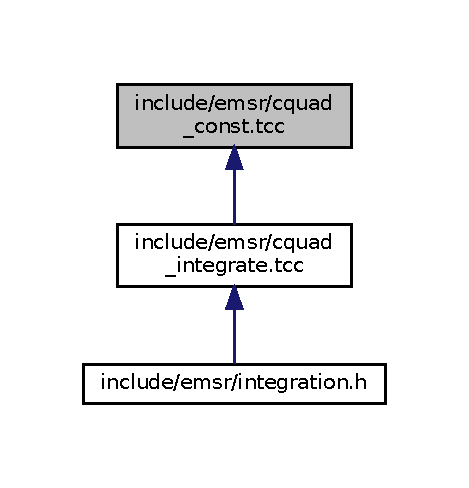
\includegraphics[width=232pt]{cquad__const_8tcc__dep__incl}
\end{center}
\end{figure}
\subsection*{Namespaces}
\begin{DoxyCompactItemize}
\item 
 \hyperlink{namespace____gnu__cxx}{\+\_\+\+\_\+gnu\+\_\+cxx}
\end{DoxyCompactItemize}
\subsection*{Macros}
\begin{DoxyCompactItemize}
\item 
\#define \hyperlink{cquad__const_8tcc_add45880010d7c8e58bc44b322ebb55c7}{C\+Q\+U\+A\+D\+\_\+\+C\+O\+N\+S\+T\+\_\+\+T\+CC}~1
\end{DoxyCompactItemize}
\subsection*{Variables}
\begin{DoxyCompactItemize}
\item 
constexpr long double \hyperlink{namespace____gnu__cxx_aad4f17907300687377704d1e628e1d70}{\+\_\+\+\_\+gnu\+\_\+cxx\+::bee} \mbox{[}68\mbox{]}
\item 
constexpr long double \hyperlink{namespace____gnu__cxx_a6a28a325aceb8d1e4e70d68b1cdeb156}{\+\_\+\+\_\+gnu\+\_\+cxx\+::\+Lalpha} \mbox{[}33\mbox{]}
\item 
constexpr long double \hyperlink{namespace____gnu__cxx_a8148a5d125951ff217becb9212005bea}{\+\_\+\+\_\+gnu\+\_\+cxx\+::\+Lgamma} \mbox{[}33\mbox{]}
\item 
constexpr long double \hyperlink{namespace____gnu__cxx_a7e499d0005aca8d0d6dd4eb30c0bc008}{\+\_\+\+\_\+gnu\+\_\+cxx\+::\+Tleft} \mbox{[}33 $\ast$33\mbox{]}
\item 
constexpr long double \hyperlink{namespace____gnu__cxx_aa35b50708b727cd96920850c90482637}{\+\_\+\+\_\+gnu\+\_\+cxx\+::\+Tright} \mbox{[}33 $\ast$33\mbox{]}
\item 
constexpr long double \hyperlink{namespace____gnu__cxx_abac562ad4a226ad8799434617959af3d}{\+\_\+\+\_\+gnu\+\_\+cxx\+::\+V1inv} \mbox{[}5 $\ast$5\mbox{]}
\item 
constexpr long double \hyperlink{namespace____gnu__cxx_aa4b649154290c645f634d501d63fac0f}{\+\_\+\+\_\+gnu\+\_\+cxx\+::\+V2inv} \mbox{[}9 $\ast$9\mbox{]}
\item 
constexpr long double \hyperlink{namespace____gnu__cxx_ac23b44065db55792c4f65364f34ee956}{\+\_\+\+\_\+gnu\+\_\+cxx\+::\+V3inv} \mbox{[}17 $\ast$17\mbox{]}
\item 
constexpr long double \hyperlink{namespace____gnu__cxx_a19b55e8c50f41d9d0a5618653f960f5c}{\+\_\+\+\_\+gnu\+\_\+cxx\+::\+V4inv} \mbox{[}33 $\ast$33\mbox{]}
\item 
constexpr long double \hyperlink{namespace____gnu__cxx_a8a912ee89c90a7e5049ce5ffad04274b}{\+\_\+\+\_\+gnu\+\_\+cxx\+::xi} \mbox{[}33\mbox{]}
\end{DoxyCompactItemize}


\subsection{Macro Definition Documentation}
\mbox{\Hypertarget{cquad__const_8tcc_add45880010d7c8e58bc44b322ebb55c7}\label{cquad__const_8tcc_add45880010d7c8e58bc44b322ebb55c7}} 
\index{cquad\+\_\+const.\+tcc@{cquad\+\_\+const.\+tcc}!C\+Q\+U\+A\+D\+\_\+\+C\+O\+N\+S\+T\+\_\+\+T\+CC@{C\+Q\+U\+A\+D\+\_\+\+C\+O\+N\+S\+T\+\_\+\+T\+CC}}
\index{C\+Q\+U\+A\+D\+\_\+\+C\+O\+N\+S\+T\+\_\+\+T\+CC@{C\+Q\+U\+A\+D\+\_\+\+C\+O\+N\+S\+T\+\_\+\+T\+CC}!cquad\+\_\+const.\+tcc@{cquad\+\_\+const.\+tcc}}
\subsubsection{\texorpdfstring{C\+Q\+U\+A\+D\+\_\+\+C\+O\+N\+S\+T\+\_\+\+T\+CC}{CQUAD\_CONST\_TCC}}
{\footnotesize\ttfamily \#define C\+Q\+U\+A\+D\+\_\+\+C\+O\+N\+S\+T\+\_\+\+T\+CC~1}



Definition at line 27 of file cquad\+\_\+const.\+tcc.


\hypertarget{cquad__integrate_8tcc}{}\doxysection{include/emsr/cquad\+\_\+integrate.tcc File Reference}
\label{cquad__integrate_8tcc}\index{include/emsr/cquad\_integrate.tcc@{include/emsr/cquad\_integrate.tcc}}
{\ttfamily \#include $<$type\+\_\+traits$>$}\newline
{\ttfamily \#include $<$emsr/cquad\+\_\+const.\+tcc$>$}\newline
{\ttfamily \#include $<$emsr/cquad\+\_\+workspace.\+h$>$}\newline
{\ttfamily \#include $<$emsr/complex\+\_\+util.\+h$>$}\newline
Include dependency graph for cquad\+\_\+integrate.\+tcc\+:
\nopagebreak
\begin{figure}[H]
\begin{center}
\leavevmode
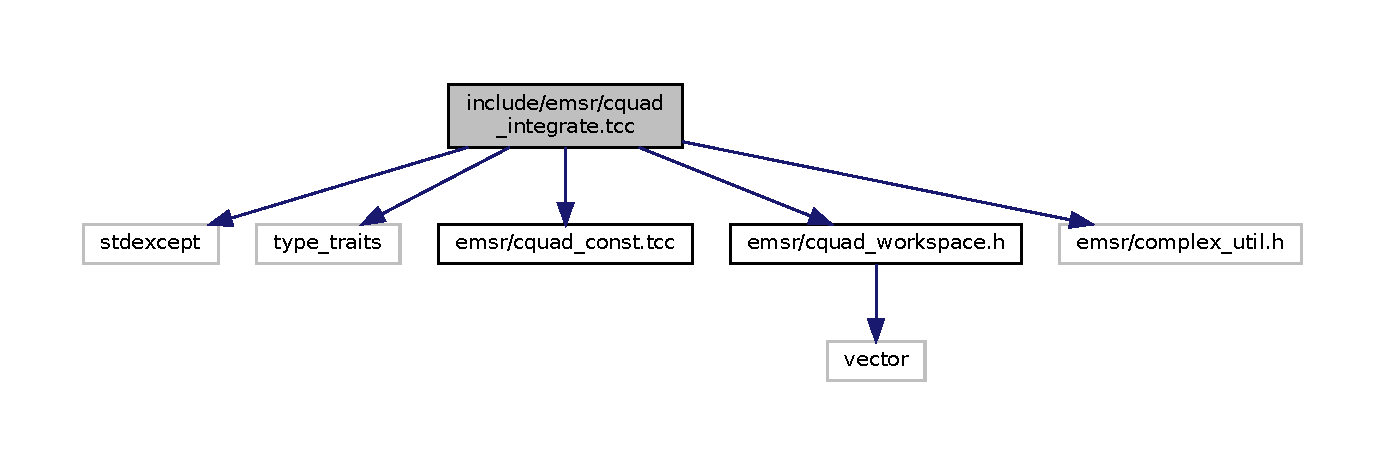
\includegraphics[width=350pt]{cquad__integrate_8tcc__incl}
\end{center}
\end{figure}
This graph shows which files directly or indirectly include this file\+:
\nopagebreak
\begin{figure}[H]
\begin{center}
\leavevmode
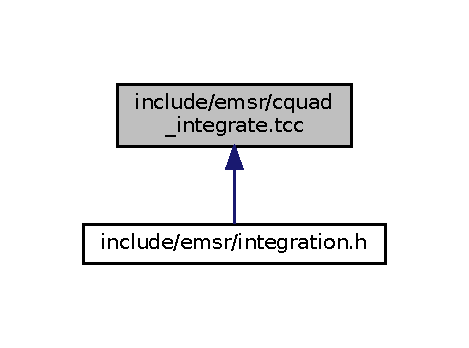
\includegraphics[width=225pt]{cquad__integrate_8tcc__dep__incl}
\end{center}
\end{figure}
\doxysubsection*{Namespaces}
\begin{DoxyCompactItemize}
\item 
 \mbox{\hyperlink{namespaceemsr}{emsr}}
\end{DoxyCompactItemize}
\doxysubsection*{Macros}
\begin{DoxyCompactItemize}
\item 
\#define \mbox{\hyperlink{cquad__integrate_8tcc_a476c60286a48a81f7de414958775fa1e}{CQUAD\+\_\+\+INTEGRATE\+\_\+\+TCC}}~1
\end{DoxyCompactItemize}
\doxysubsection*{Functions}
\begin{DoxyCompactItemize}
\item 
{\footnotesize template$<$typename Tp , typename Func\+Tp $>$ }\\auto \mbox{\hyperlink{namespaceemsr_a33dbcaf38f3b561a02fef8f77cc95797}{emsr\+::cquad\+\_\+integrate}} (cquad\+\_\+workspace$<$ \mbox{\hyperlink{test__integral_8tcc_a82f489a4943d33943d0b0f781a801283}{Tp}}, std\+::invoke\+\_\+result\+\_\+t$<$ Func\+Tp, \mbox{\hyperlink{test__integral_8tcc_a82f489a4943d33943d0b0f781a801283}{Tp}} $>$$>$ \&ws, Func\+Tp func, \mbox{\hyperlink{test__integral_8tcc_a82f489a4943d33943d0b0f781a801283}{Tp}} a, \mbox{\hyperlink{test__integral_8tcc_a82f489a4943d33943d0b0f781a801283}{Tp}} b, \mbox{\hyperlink{test__integral_8tcc_a82f489a4943d33943d0b0f781a801283}{Tp}} epsabs, \mbox{\hyperlink{test__integral_8tcc_a82f489a4943d33943d0b0f781a801283}{Tp}} epsrel) -\/$>$ adaptive\+\_\+integral\+\_\+t$<$ \mbox{\hyperlink{test__integral_8tcc_a82f489a4943d33943d0b0f781a801283}{Tp}}, std\+::invoke\+\_\+result\+\_\+t$<$ Func\+Tp, \mbox{\hyperlink{test__integral_8tcc_a82f489a4943d33943d0b0f781a801283}{Tp}} $>$$>$
\item 
{\footnotesize template$<$typename Tp $>$ }\\void \mbox{\hyperlink{namespaceemsr_ada0a5521139a0380c69060f9a8bdbda7}{emsr\+::downdate}} (\mbox{\hyperlink{test__integral_8tcc_a82f489a4943d33943d0b0f781a801283}{Tp}} $\ast$coeff, std\+::ptrdiff\+\_\+t n, std\+::ptrdiff\+\_\+t depth, std\+::ptrdiff\+\_\+t $\ast$NaN, std\+::ptrdiff\+\_\+t num\+\_\+\+Na\+Ns)
\item 
{\footnotesize template$<$typename Ret\+Tp $>$ }\\void \mbox{\hyperlink{namespaceemsr_ad4641c4c152fbc43029f47a4d80c77e9}{emsr\+::\+Vinvfx}} (const std\+::array$<$ Ret\+Tp, 33 $>$ \&fx, Ret\+Tp $\ast$coeff, const int depth)
\end{DoxyCompactItemize}


\doxysubsection{Macro Definition Documentation}
\mbox{\Hypertarget{cquad__integrate_8tcc_a476c60286a48a81f7de414958775fa1e}\label{cquad__integrate_8tcc_a476c60286a48a81f7de414958775fa1e}} 
\index{cquad\_integrate.tcc@{cquad\_integrate.tcc}!CQUAD\_INTEGRATE\_TCC@{CQUAD\_INTEGRATE\_TCC}}
\index{CQUAD\_INTEGRATE\_TCC@{CQUAD\_INTEGRATE\_TCC}!cquad\_integrate.tcc@{cquad\_integrate.tcc}}
\doxysubsubsection{\texorpdfstring{CQUAD\_INTEGRATE\_TCC}{CQUAD\_INTEGRATE\_TCC}}
{\footnotesize\ttfamily \#define CQUAD\+\_\+\+INTEGRATE\+\_\+\+TCC~1}



Definition at line 27 of file cquad\+\_\+integrate.\+tcc.


\hypertarget{cquad__workspace_8h}{}\doxysection{include/emsr/cquad\+\_\+workspace.h File Reference}
\label{cquad__workspace_8h}\index{include/emsr/cquad\_workspace.h@{include/emsr/cquad\_workspace.h}}
{\ttfamily \#include $<$vector$>$}\newline
Include dependency graph for cquad\+\_\+workspace.\+h\+:
\nopagebreak
\begin{figure}[H]
\begin{center}
\leavevmode
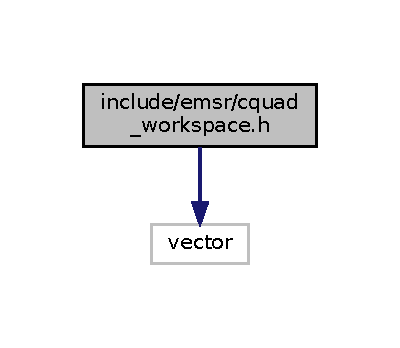
\includegraphics[width=192pt]{cquad__workspace_8h__incl}
\end{center}
\end{figure}
This graph shows which files directly or indirectly include this file\+:
\nopagebreak
\begin{figure}[H]
\begin{center}
\leavevmode
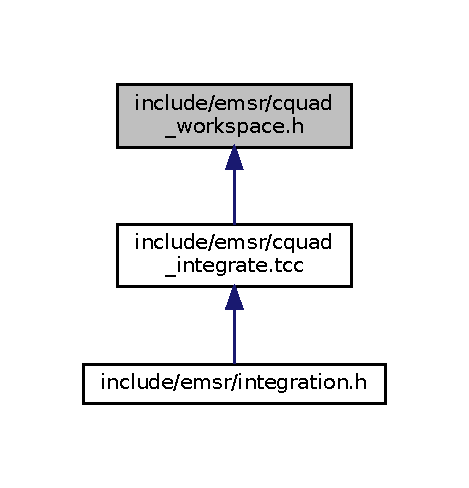
\includegraphics[width=225pt]{cquad__workspace_8h__dep__incl}
\end{center}
\end{figure}
\doxysubsection*{Classes}
\begin{DoxyCompactItemize}
\item 
struct \mbox{\hyperlink{structemsr_1_1cquad__interval}{emsr\+::cquad\+\_\+interval$<$ Tp, Ret\+Tp $>$}}
\item 
struct \mbox{\hyperlink{structemsr_1_1cquad__interval__comp}{emsr\+::cquad\+\_\+interval\+\_\+comp$<$ Tp, Ret\+Tp $>$}}
\item 
struct \mbox{\hyperlink{structemsr_1_1cquad__workspace}{emsr\+::cquad\+\_\+workspace$<$ Tp, Ret\+Tp $>$}}
\end{DoxyCompactItemize}
\doxysubsection*{Namespaces}
\begin{DoxyCompactItemize}
\item 
 \mbox{\hyperlink{namespaceemsr}{emsr}}
\end{DoxyCompactItemize}
\doxysubsection*{Functions}
\begin{DoxyCompactItemize}
\item 
{\footnotesize template$<$typename Tp , typename Ret\+Tp $>$ }\\bool \mbox{\hyperlink{namespaceemsr_a362d779420728a72a7f3ff944d109280}{emsr\+::operator$<$}} (const cquad\+\_\+interval$<$ \mbox{\hyperlink{test__integral_8tcc_a82f489a4943d33943d0b0f781a801283}{Tp}}, Ret\+Tp $>$ \&ivl, const cquad\+\_\+interval$<$ \mbox{\hyperlink{test__integral_8tcc_a82f489a4943d33943d0b0f781a801283}{Tp}}, Ret\+Tp $>$ \&ivr)
\end{DoxyCompactItemize}

\hypertarget{double__exp__integrate_8tcc}{}\doxysection{include/emsr/double\+\_\+exp\+\_\+integrate.tcc File Reference}
\label{double__exp__integrate_8tcc}\index{include/emsr/double\_exp\_integrate.tcc@{include/emsr/double\_exp\_integrate.tcc}}
{\ttfamily \#include $<$type\+\_\+traits$>$}\newline
{\ttfamily \#include $<$cmath$>$}\newline
Include dependency graph for double\+\_\+exp\+\_\+integrate.\+tcc\+:
\nopagebreak
\begin{figure}[H]
\begin{center}
\leavevmode
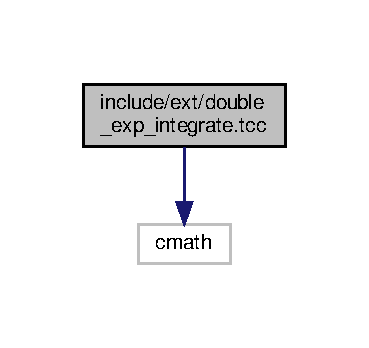
\includegraphics[width=214pt]{double__exp__integrate_8tcc__incl}
\end{center}
\end{figure}
This graph shows which files directly or indirectly include this file\+:
\nopagebreak
\begin{figure}[H]
\begin{center}
\leavevmode
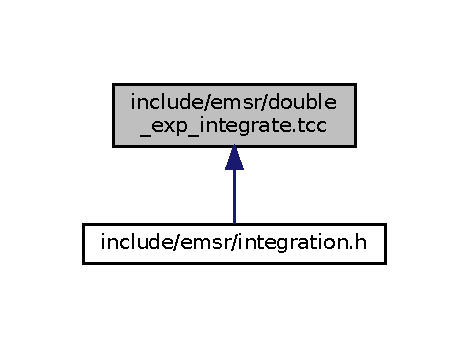
\includegraphics[width=225pt]{double__exp__integrate_8tcc__dep__incl}
\end{center}
\end{figure}
\doxysubsection*{Namespaces}
\begin{DoxyCompactItemize}
\item 
 \mbox{\hyperlink{namespaceemsr}{emsr}}
\end{DoxyCompactItemize}
\doxysubsection*{Macros}
\begin{DoxyCompactItemize}
\item 
\#define \mbox{\hyperlink{double__exp__integrate_8tcc_a939b63d0839d3b313a4f6b094d3ea9e9}{DOUBLE\+\_\+\+EXP\+\_\+\+INTEGRATE\+\_\+\+TCC}}~1
\end{DoxyCompactItemize}
\doxysubsection*{Functions}
\begin{DoxyCompactItemize}
\item 
{\footnotesize template$<$typename Tp , typename Func\+Tp $>$ }\\adaptive\+\_\+integral\+\_\+t$<$ \mbox{\hyperlink{test__integral_8tcc_a82f489a4943d33943d0b0f781a801283}{Tp}}, std\+::invoke\+\_\+result\+\_\+t$<$ Func\+Tp, \mbox{\hyperlink{test__integral_8tcc_a82f489a4943d33943d0b0f781a801283}{Tp}} $>$ $>$ \mbox{\hyperlink{namespaceemsr_a2d0acef208b396614990effbe15a81af}{emsr\+::integrate\+\_\+exp\+\_\+sinh}} (Func\+Tp func, \mbox{\hyperlink{test__integral_8tcc_a82f489a4943d33943d0b0f781a801283}{Tp}} lower, \mbox{\hyperlink{test__integral_8tcc_a82f489a4943d33943d0b0f781a801283}{Tp}} max\+\_\+abs\+\_\+err, \mbox{\hyperlink{test__integral_8tcc_a82f489a4943d33943d0b0f781a801283}{Tp}} max\+\_\+rel\+\_\+err, int max\+\_\+iter)
\item 
{\footnotesize template$<$typename Tp , typename Func\+Tp $>$ }\\adaptive\+\_\+integral\+\_\+t$<$ \mbox{\hyperlink{test__integral_8tcc_a82f489a4943d33943d0b0f781a801283}{Tp}}, std\+::invoke\+\_\+result\+\_\+t$<$ Func\+Tp, \mbox{\hyperlink{test__integral_8tcc_a82f489a4943d33943d0b0f781a801283}{Tp}} $>$ $>$ \mbox{\hyperlink{namespaceemsr_a52c236f1ff64f5f2370c8520d250c447}{emsr\+::integrate\+\_\+sinh\+\_\+sinh}} (Func\+Tp func, \mbox{\hyperlink{test__integral_8tcc_a82f489a4943d33943d0b0f781a801283}{Tp}} max\+\_\+abs\+\_\+err, \mbox{\hyperlink{test__integral_8tcc_a82f489a4943d33943d0b0f781a801283}{Tp}} max\+\_\+rel\+\_\+err, int max\+\_\+iter)
\item 
{\footnotesize template$<$typename Tp , typename Func\+Tp $>$ }\\adaptive\+\_\+integral\+\_\+t$<$ \mbox{\hyperlink{test__integral_8tcc_a82f489a4943d33943d0b0f781a801283}{Tp}}, std\+::invoke\+\_\+result\+\_\+t$<$ Func\+Tp, \mbox{\hyperlink{test__integral_8tcc_a82f489a4943d33943d0b0f781a801283}{Tp}} $>$ $>$ \mbox{\hyperlink{namespaceemsr_a933d086ea58a17c690e3eaca8655e009}{emsr\+::integrate\+\_\+tanh\+\_\+sinh}} (Func\+Tp func, \mbox{\hyperlink{test__integral_8tcc_a82f489a4943d33943d0b0f781a801283}{Tp}} lower, \mbox{\hyperlink{test__integral_8tcc_a82f489a4943d33943d0b0f781a801283}{Tp}} upper, \mbox{\hyperlink{test__integral_8tcc_a82f489a4943d33943d0b0f781a801283}{Tp}} max\+\_\+abs\+\_\+err, \mbox{\hyperlink{test__integral_8tcc_a82f489a4943d33943d0b0f781a801283}{Tp}} max\+\_\+rel\+\_\+err, int max\+\_\+iter)
\end{DoxyCompactItemize}


\doxysubsection{Macro Definition Documentation}
\mbox{\Hypertarget{double__exp__integrate_8tcc_a939b63d0839d3b313a4f6b094d3ea9e9}\label{double__exp__integrate_8tcc_a939b63d0839d3b313a4f6b094d3ea9e9}} 
\index{double\_exp\_integrate.tcc@{double\_exp\_integrate.tcc}!DOUBLE\_EXP\_INTEGRATE\_TCC@{DOUBLE\_EXP\_INTEGRATE\_TCC}}
\index{DOUBLE\_EXP\_INTEGRATE\_TCC@{DOUBLE\_EXP\_INTEGRATE\_TCC}!double\_exp\_integrate.tcc@{double\_exp\_integrate.tcc}}
\doxysubsubsection{\texorpdfstring{DOUBLE\_EXP\_INTEGRATE\_TCC}{DOUBLE\_EXP\_INTEGRATE\_TCC}}
{\footnotesize\ttfamily \#define DOUBLE\+\_\+\+EXP\+\_\+\+INTEGRATE\+\_\+\+TCC~1}



Definition at line 21 of file double\+\_\+exp\+\_\+integrate.\+tcc.


\hypertarget{extrapolation__table_8h}{}\section{include/ext/extrapolation\+\_\+table.h File Reference}
\label{extrapolation__table_8h}\index{include/ext/extrapolation\+\_\+table.\+h@{include/ext/extrapolation\+\_\+table.\+h}}
{\ttfamily \#include $<$array$>$}\newline
{\ttfamily \#include $<$utility$>$}\newline
{\ttfamily \#include $<$limits$>$}\newline
{\ttfamily \#include $<$cmath$>$}\newline
{\ttfamily \#include $<$algorithm$>$}\newline
{\ttfamily \#include $<$ext/extrapolation\+\_\+table.\+tcc$>$}\newline
Include dependency graph for extrapolation\+\_\+table.\+h\+:
\nopagebreak
\begin{figure}[H]
\begin{center}
\leavevmode
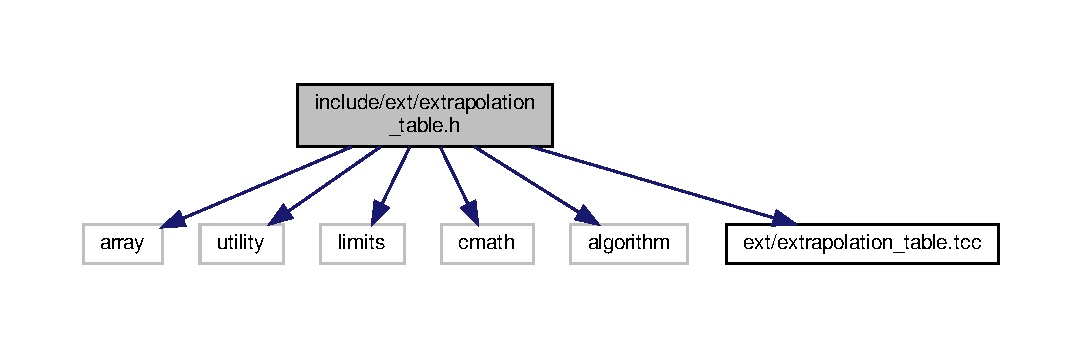
\includegraphics[width=350pt]{extrapolation__table_8h__incl}
\end{center}
\end{figure}
This graph shows which files directly or indirectly include this file\+:
\nopagebreak
\begin{figure}[H]
\begin{center}
\leavevmode
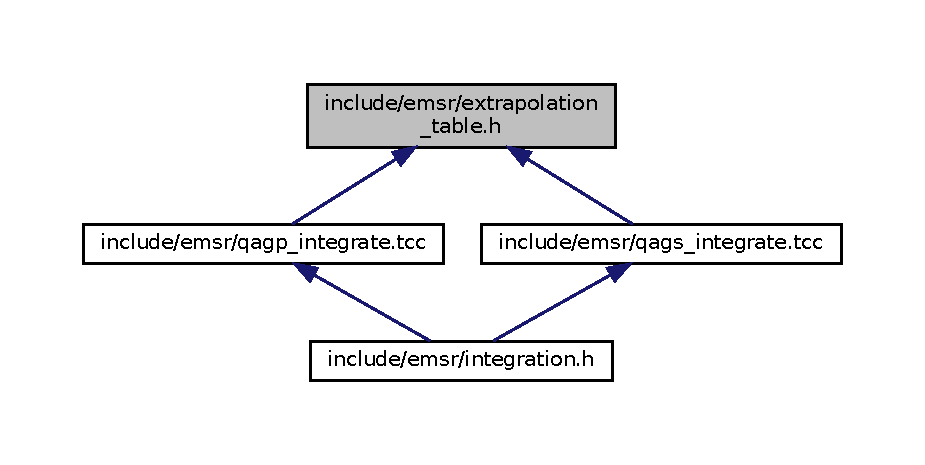
\includegraphics[width=350pt]{extrapolation__table_8h__dep__incl}
\end{center}
\end{figure}
\subsection*{Classes}
\begin{DoxyCompactItemize}
\item 
class \hyperlink{class____gnu__cxx_1_1extrapolation__table}{\+\_\+\+\_\+gnu\+\_\+cxx\+::extrapolation\+\_\+table$<$ \+\_\+\+Tp $>$}
\end{DoxyCompactItemize}
\subsection*{Namespaces}
\begin{DoxyCompactItemize}
\item 
 \hyperlink{namespace____gnu__cxx}{\+\_\+\+\_\+gnu\+\_\+cxx}
\end{DoxyCompactItemize}

\hypertarget{extrapolation__table_8tcc}{}\section{include/ext/extrapolation\+\_\+table.tcc File Reference}
\label{extrapolation__table_8tcc}\index{include/ext/extrapolation\+\_\+table.\+tcc@{include/ext/extrapolation\+\_\+table.\+tcc}}
This graph shows which files directly or indirectly include this file\+:
\nopagebreak
\begin{figure}[H]
\begin{center}
\leavevmode
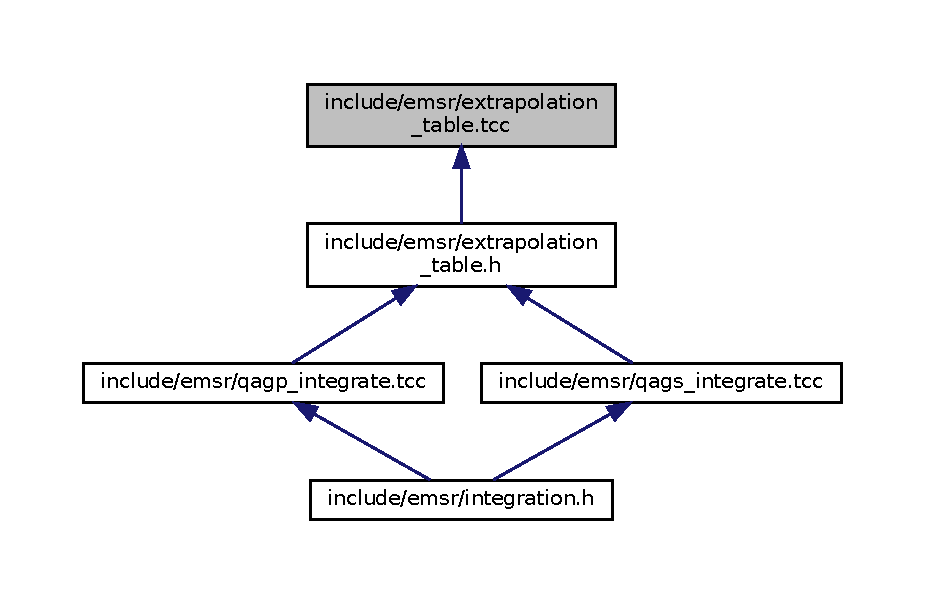
\includegraphics[width=350pt]{extrapolation__table_8tcc__dep__incl}
\end{center}
\end{figure}
\subsection*{Namespaces}
\begin{DoxyCompactItemize}
\item 
 \hyperlink{namespace____gnu__cxx}{\+\_\+\+\_\+gnu\+\_\+cxx}
\end{DoxyCompactItemize}
\subsection*{Macros}
\begin{DoxyCompactItemize}
\item 
\#define \hyperlink{extrapolation__table_8tcc_ab99f24f7cb464f1e3ae40b745db8df16}{E\+X\+T\+R\+A\+P\+O\+L\+A\+T\+I\+O\+N\+\_\+\+T\+A\+B\+L\+E\+\_\+\+T\+CC}~1
\end{DoxyCompactItemize}


\subsection{Macro Definition Documentation}
\mbox{\Hypertarget{extrapolation__table_8tcc_ab99f24f7cb464f1e3ae40b745db8df16}\label{extrapolation__table_8tcc_ab99f24f7cb464f1e3ae40b745db8df16}} 
\index{extrapolation\+\_\+table.\+tcc@{extrapolation\+\_\+table.\+tcc}!E\+X\+T\+R\+A\+P\+O\+L\+A\+T\+I\+O\+N\+\_\+\+T\+A\+B\+L\+E\+\_\+\+T\+CC@{E\+X\+T\+R\+A\+P\+O\+L\+A\+T\+I\+O\+N\+\_\+\+T\+A\+B\+L\+E\+\_\+\+T\+CC}}
\index{E\+X\+T\+R\+A\+P\+O\+L\+A\+T\+I\+O\+N\+\_\+\+T\+A\+B\+L\+E\+\_\+\+T\+CC@{E\+X\+T\+R\+A\+P\+O\+L\+A\+T\+I\+O\+N\+\_\+\+T\+A\+B\+L\+E\+\_\+\+T\+CC}!extrapolation\+\_\+table.\+tcc@{extrapolation\+\_\+table.\+tcc}}
\subsubsection{\texorpdfstring{E\+X\+T\+R\+A\+P\+O\+L\+A\+T\+I\+O\+N\+\_\+\+T\+A\+B\+L\+E\+\_\+\+T\+CC}{EXTRAPOLATION\_TABLE\_TCC}}
{\footnotesize\ttfamily \#define E\+X\+T\+R\+A\+P\+O\+L\+A\+T\+I\+O\+N\+\_\+\+T\+A\+B\+L\+E\+\_\+\+T\+CC~1}



Definition at line 28 of file extrapolation\+\_\+table.\+tcc.


\hypertarget{fourier__transform_8h}{}\doxysection{include/emsr/fourier\+\_\+transform.h File Reference}
\label{fourier__transform_8h}\index{include/emsr/fourier\_transform.h@{include/emsr/fourier\_transform.h}}
{\ttfamily \#include $<$complex$>$}\newline
{\ttfamily \#include $<$vector$>$}\newline
{\ttfamily \#include $<$emsr/fourier\+\_\+transform.\+tcc$>$}\newline
Include dependency graph for fourier\+\_\+transform.\+h\+:
\nopagebreak
\begin{figure}[H]
\begin{center}
\leavevmode
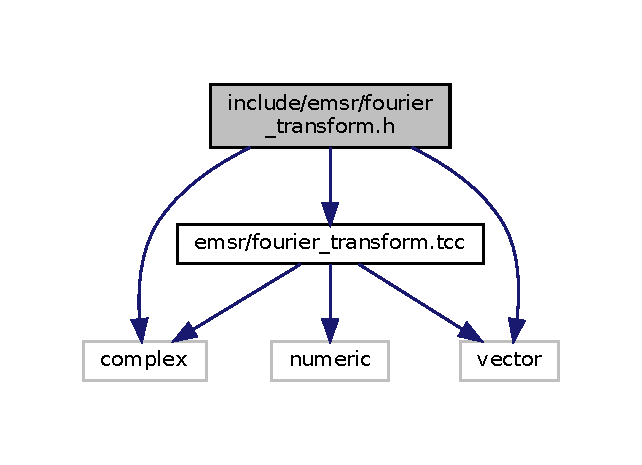
\includegraphics[width=308pt]{fourier__transform_8h__incl}
\end{center}
\end{figure}
\doxysubsection*{Classes}
\begin{DoxyCompactItemize}
\item 
class \mbox{\hyperlink{classemsr_1_1fourier__transform__t}{emsr\+::fourier\+\_\+transform\+\_\+t$<$ Tp $>$}}
\item 
class \mbox{\hyperlink{classemsr_1_1fourier__transform__t_3_01std_1_1complex_3_01Tp_01_4_01_4}{emsr\+::fourier\+\_\+transform\+\_\+t$<$ std\+::complex$<$ Tp $>$ $>$}}
\item 
class \mbox{\hyperlink{classemsr_1_1phase__iterator}{emsr\+::phase\+\_\+iterator$<$ Tp $>$}}
\end{DoxyCompactItemize}
\doxysubsection*{Namespaces}
\begin{DoxyCompactItemize}
\item 
 \mbox{\hyperlink{namespaceemsr}{emsr}}
\end{DoxyCompactItemize}
\doxysubsection*{Functions}
\begin{DoxyCompactItemize}
\item 
{\footnotesize template$<$typename Tp $>$ }\\void \mbox{\hyperlink{namespaceemsr_a6d214674e0f0a97431252c6f7774c2d2}{emsr\+::discrete\+\_\+fourier\+\_\+transform}} (bool do\+\_\+forward, std\+::vector$<$ std\+::complex$<$ \mbox{\hyperlink{test__integral_8tcc_a82f489a4943d33943d0b0f781a801283}{Tp}} $>$$>$ \&z)
\item 
{\footnotesize template$<$typename Cmplx\+Iter $>$ }\\void \mbox{\hyperlink{namespaceemsr_a46477280c3e50f2030980ee67021563a}{emsr\+::fast\+\_\+fourier\+\_\+transform}} (const Cmplx\+Iter \&from, const Cmplx\+Iter \&to)
\item 
{\footnotesize template$<$typename Tp $>$ }\\void \mbox{\hyperlink{namespaceemsr_a21a5616f82ab27740a356502f30d7f5c}{emsr\+::fast\+\_\+fourier\+\_\+transform}} (std\+::vector$<$ std\+::complex$<$ \mbox{\hyperlink{test__integral_8tcc_a82f489a4943d33943d0b0f781a801283}{Tp}} $>$$>$ \&z)
\item 
{\footnotesize template$<$typename Tp $>$ }\\void \mbox{\hyperlink{namespaceemsr_a97d70c270cd3edc86cae06066f7be627}{emsr\+::fast\+\_\+fourier\+\_\+transform}} (std\+::vector$<$ \mbox{\hyperlink{test__integral_8tcc_a82f489a4943d33943d0b0f781a801283}{Tp}} $>$ \&x)
\item 
{\footnotesize template$<$typename Tp $>$ }\\void \mbox{\hyperlink{namespaceemsr_a0326d2943aad38911efc741e8bfa3da3}{emsr\+::fast\+\_\+sine\+\_\+transform}} (std\+::vector$<$ \mbox{\hyperlink{test__integral_8tcc_a82f489a4943d33943d0b0f781a801283}{Tp}} $>$ \&x)
\item 
{\footnotesize template$<$typename Cmplx\+Iter $>$ }\\void \mbox{\hyperlink{namespaceemsr_a4b1e7785cbd6c324e4744ea04a6a6ed9}{emsr\+::inv\+\_\+fast\+\_\+fourier\+\_\+transform}} (const Cmplx\+Iter \&from, const Cmplx\+Iter \&to)
\item 
{\footnotesize template$<$typename Tp $>$ }\\void \mbox{\hyperlink{namespaceemsr_a30e888750ec6fb0b624937e1301a3984}{emsr\+::inv\+\_\+fast\+\_\+fourier\+\_\+transform}} (std\+::vector$<$ std\+::complex$<$ \mbox{\hyperlink{test__integral_8tcc_a82f489a4943d33943d0b0f781a801283}{Tp}} $>$$>$ \&z)
\item 
{\footnotesize template$<$typename Tp $>$ }\\void \mbox{\hyperlink{namespaceemsr_a731e24ac69081b4c39dbe81b05f905f1}{emsr\+::inv\+\_\+fast\+\_\+fourier\+\_\+transform}} (std\+::vector$<$ \mbox{\hyperlink{test__integral_8tcc_a82f489a4943d33943d0b0f781a801283}{Tp}} $>$ \&x)
\item 
{\footnotesize template$<$typename Tp $>$ }\\void \mbox{\hyperlink{namespaceemsr_a4b3d1c02a910253093ea8560e4baea0a}{emsr\+::inv\+\_\+fast\+\_\+sine\+\_\+transform}} (std\+::vector$<$ \mbox{\hyperlink{test__integral_8tcc_a82f489a4943d33943d0b0f781a801283}{Tp}} $>$ \&x)
\end{DoxyCompactItemize}

\hypertarget{fourier__transform_8tcc}{}\section{include/ext/fourier\+\_\+transform.tcc File Reference}
\label{fourier__transform_8tcc}\index{include/ext/fourier\+\_\+transform.\+tcc@{include/ext/fourier\+\_\+transform.\+tcc}}
{\ttfamily \#include $<$numeric$>$}\newline
{\ttfamily \#include $<$vector$>$}\newline
{\ttfamily \#include $<$complex$>$}\newline
Include dependency graph for fourier\+\_\+transform.\+tcc\+:
\nopagebreak
\begin{figure}[H]
\begin{center}
\leavevmode
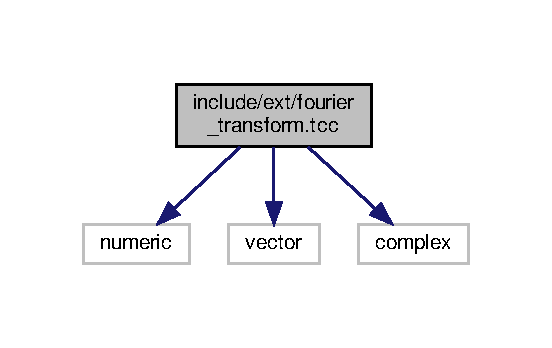
\includegraphics[width=265pt]{fourier__transform_8tcc__incl}
\end{center}
\end{figure}
This graph shows which files directly or indirectly include this file\+:
\nopagebreak
\begin{figure}[H]
\begin{center}
\leavevmode
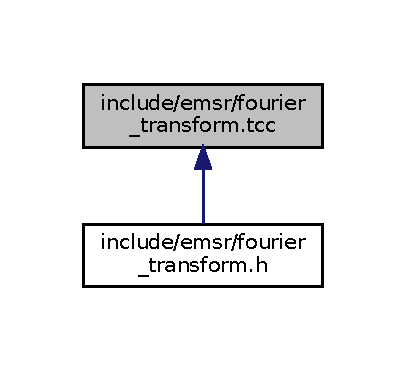
\includegraphics[width=174pt]{fourier__transform_8tcc__dep__incl}
\end{center}
\end{figure}
\subsection*{Namespaces}
\begin{DoxyCompactItemize}
\item 
 \hyperlink{namespace____gnu__cxx}{\+\_\+\+\_\+gnu\+\_\+cxx}
\end{DoxyCompactItemize}
\subsection*{Macros}
\begin{DoxyCompactItemize}
\item 
\#define \hyperlink{fourier__transform_8tcc_a14631aeeab3dded5b6dcf462996933c3}{F\+O\+U\+R\+I\+E\+R\+\_\+\+T\+R\+A\+N\+S\+F\+O\+R\+M\+\_\+\+T\+CC}~1
\end{DoxyCompactItemize}
\subsection*{Functions}
\begin{DoxyCompactItemize}
\item 
{\footnotesize template$<$typename \+\_\+\+Tp $>$ }\\void \hyperlink{namespace____gnu__cxx_a6dff31b609fa2f8678c729d557dbae49}{\+\_\+\+\_\+gnu\+\_\+cxx\+::\+\_\+\+\_\+discrete\+\_\+fourier\+\_\+transform} (bool \+\_\+\+\_\+do\+\_\+forward, std\+::vector$<$ std\+::complex$<$ \+\_\+\+Tp $>$$>$ \&\+\_\+\+\_\+z)
\item 
{\footnotesize template$<$typename \+\_\+\+Tp $>$ }\\void \hyperlink{namespace____gnu__cxx_a64fbc0765e55d7466a21baa9f652362e}{\+\_\+\+\_\+gnu\+\_\+cxx\+::fast\+\_\+fourier\+\_\+transform} (std\+::vector$<$ std\+::complex$<$ \+\_\+\+Tp $>$$>$ \&\+\_\+\+\_\+z)
\item 
{\footnotesize template$<$typename \+\_\+\+Tp $>$ }\\void \hyperlink{namespace____gnu__cxx_ae6b377214391002ca75ca712823fd45c}{\+\_\+\+\_\+gnu\+\_\+cxx\+::fast\+\_\+fourier\+\_\+transform} (std\+::vector$<$ \+\_\+\+Tp $>$ \&\+\_\+\+\_\+x)
\item 
{\footnotesize template$<$typename \+\_\+\+Cmplx\+Iter $>$ }\\void \hyperlink{namespace____gnu__cxx_a8e1dab366323a810c9915329b520aa5a}{\+\_\+\+\_\+gnu\+\_\+cxx\+::fast\+\_\+fourier\+\_\+transform} (const \+\_\+\+Cmplx\+Iter \&\+\_\+\+\_\+from, const \+\_\+\+Cmplx\+Iter \&\+\_\+\+\_\+to)
\item 
{\footnotesize template$<$typename \+\_\+\+Tp $>$ }\\void \hyperlink{namespace____gnu__cxx_a97f96274ac4998cf6a7c37fcb48c9bff}{\+\_\+\+\_\+gnu\+\_\+cxx\+::fast\+\_\+sine\+\_\+transform} (std\+::vector$<$ \+\_\+\+Tp $>$ \&\+\_\+\+\_\+x)
\item 
{\footnotesize template$<$typename \+\_\+\+Tp $>$ }\\void \hyperlink{namespace____gnu__cxx_a96b56c927599a614656027d3ab4b82ac}{\+\_\+\+\_\+gnu\+\_\+cxx\+::inv\+\_\+fast\+\_\+fourier\+\_\+transform} (std\+::vector$<$ std\+::complex$<$ \+\_\+\+Tp $>$$>$ \&\+\_\+\+\_\+z)
\item 
{\footnotesize template$<$typename \+\_\+\+Tp $>$ }\\void \hyperlink{namespace____gnu__cxx_a1fe4b25c379855d94a657b688a327e80}{\+\_\+\+\_\+gnu\+\_\+cxx\+::inv\+\_\+fast\+\_\+fourier\+\_\+transform} (std\+::vector$<$ \+\_\+\+Tp $>$ \&\+\_\+\+\_\+x)
\item 
{\footnotesize template$<$typename \+\_\+\+Cmplx\+Iter $>$ }\\void \hyperlink{namespace____gnu__cxx_a98a4b1edde28198a694042bea78da893}{\+\_\+\+\_\+gnu\+\_\+cxx\+::inv\+\_\+fast\+\_\+fourier\+\_\+transform} (const \+\_\+\+Cmplx\+Iter \&\+\_\+\+\_\+from, const \+\_\+\+Cmplx\+Iter \&\+\_\+\+\_\+to)
\item 
{\footnotesize template$<$typename \+\_\+\+Tp $>$ }\\void \hyperlink{namespace____gnu__cxx_a71c4de302fa0b6716f936d2d925352bd}{\+\_\+\+\_\+gnu\+\_\+cxx\+::inv\+\_\+fast\+\_\+sine\+\_\+transform} (std\+::vector$<$ \+\_\+\+Tp $>$ \&\+\_\+\+\_\+x)
\end{DoxyCompactItemize}


\subsection{Macro Definition Documentation}
\mbox{\Hypertarget{fourier__transform_8tcc_a14631aeeab3dded5b6dcf462996933c3}\label{fourier__transform_8tcc_a14631aeeab3dded5b6dcf462996933c3}} 
\index{fourier\+\_\+transform.\+tcc@{fourier\+\_\+transform.\+tcc}!F\+O\+U\+R\+I\+E\+R\+\_\+\+T\+R\+A\+N\+S\+F\+O\+R\+M\+\_\+\+T\+CC@{F\+O\+U\+R\+I\+E\+R\+\_\+\+T\+R\+A\+N\+S\+F\+O\+R\+M\+\_\+\+T\+CC}}
\index{F\+O\+U\+R\+I\+E\+R\+\_\+\+T\+R\+A\+N\+S\+F\+O\+R\+M\+\_\+\+T\+CC@{F\+O\+U\+R\+I\+E\+R\+\_\+\+T\+R\+A\+N\+S\+F\+O\+R\+M\+\_\+\+T\+CC}!fourier\+\_\+transform.\+tcc@{fourier\+\_\+transform.\+tcc}}
\subsubsection{\texorpdfstring{F\+O\+U\+R\+I\+E\+R\+\_\+\+T\+R\+A\+N\+S\+F\+O\+R\+M\+\_\+\+T\+CC}{FOURIER\_TRANSFORM\_TCC}}
{\footnotesize\ttfamily \#define F\+O\+U\+R\+I\+E\+R\+\_\+\+T\+R\+A\+N\+S\+F\+O\+R\+M\+\_\+\+T\+CC~1}



Definition at line 22 of file fourier\+\_\+transform.\+tcc.


\hypertarget{gauss__hermite__integrate_8h}{}\section{include/ext/gauss\+\_\+hermite\+\_\+integrate.h File Reference}
\label{gauss__hermite__integrate_8h}\index{include/ext/gauss\+\_\+hermite\+\_\+integrate.\+h@{include/ext/gauss\+\_\+hermite\+\_\+integrate.\+h}}
{\ttfamily \#include $<$vector$>$}\newline
Include dependency graph for gauss\+\_\+hermite\+\_\+integrate.\+h\+:
\nopagebreak
\begin{figure}[H]
\begin{center}
\leavevmode
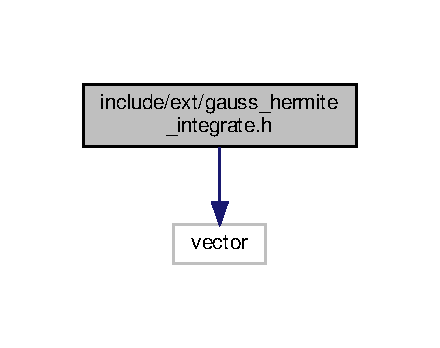
\includegraphics[width=211pt]{gauss__hermite__integrate_8h__incl}
\end{center}
\end{figure}
\subsection*{Namespaces}
\begin{DoxyCompactItemize}
\item 
 \hyperlink{namespace____gnu__cxx}{\+\_\+\+\_\+gnu\+\_\+cxx}
\end{DoxyCompactItemize}
\subsection*{Variables}
\begin{DoxyCompactItemize}
\item 
{\footnotesize template$<$typename \+\_\+\+Tp , typename \+\_\+\+Func $>$ }\\decltype(std\+::invoke\+\_\+result\+\_\+t$<$ \+\_\+\+Func, \+\_\+\+Tp $>$\{\} $\ast$\+\_\+\+Tp\{\} \hyperlink{namespace____gnu__cxx_a0e320b6b2f1b1befb9019e587648534d}{\+\_\+\+\_\+gnu\+\_\+cxx\+::gauss\+\_\+hermite\+\_\+integrate} )(\+\_\+\+Func \+\_\+\+\_\+func, unsigned int \+\_\+\+\_\+n)
\end{DoxyCompactItemize}

\hypertarget{gauss__jacobi__integrate_8tcc}{}\doxysection{include/emsr/gauss\+\_\+jacobi\+\_\+integrate.tcc File Reference}
\label{gauss__jacobi__integrate_8tcc}\index{include/emsr/gauss\_jacobi\_integrate.tcc@{include/emsr/gauss\_jacobi\_integrate.tcc}}
{\ttfamily \#include $<$cmath$>$}\newline
{\ttfamily \#include $<$cstdlib$>$}\newline
{\ttfamily \#include $<$cstdio$>$}\newline
{\ttfamily \#include $<$limits$>$}\newline
{\ttfamily \#include $<$ext/jacobi.\+h$>$}\newline
{\ttfamily \#include $<$ext/integration\+\_\+error.\+h$>$}\newline
Include dependency graph for gauss\+\_\+jacobi\+\_\+integrate.\+tcc\+:
\nopagebreak
\begin{figure}[H]
\begin{center}
\leavevmode
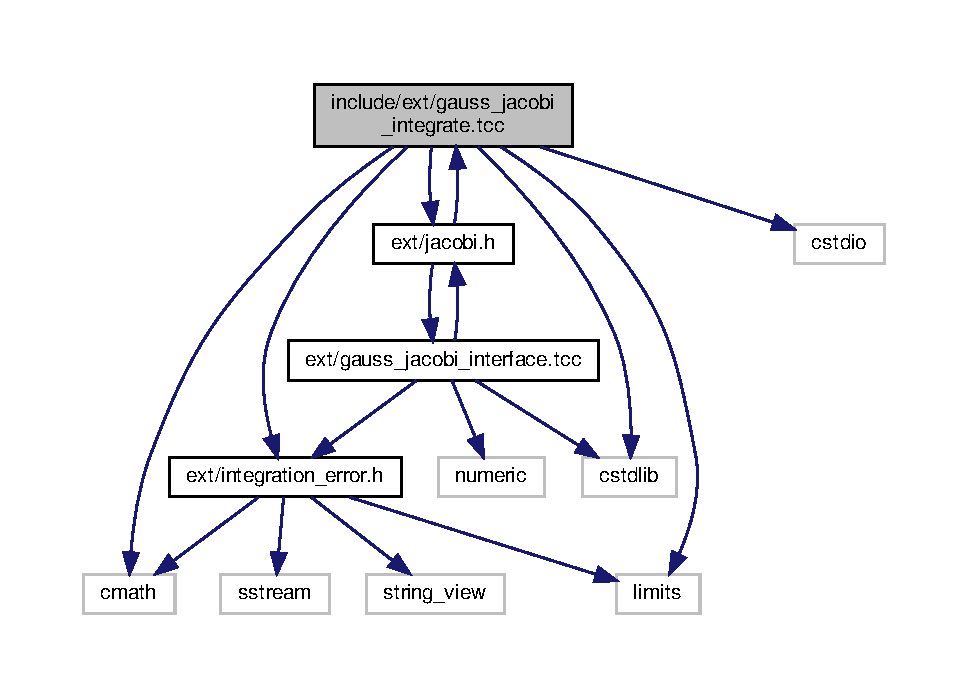
\includegraphics[width=350pt]{gauss__jacobi__integrate_8tcc__incl}
\end{center}
\end{figure}
This graph shows which files directly or indirectly include this file\+:
\nopagebreak
\begin{figure}[H]
\begin{center}
\leavevmode
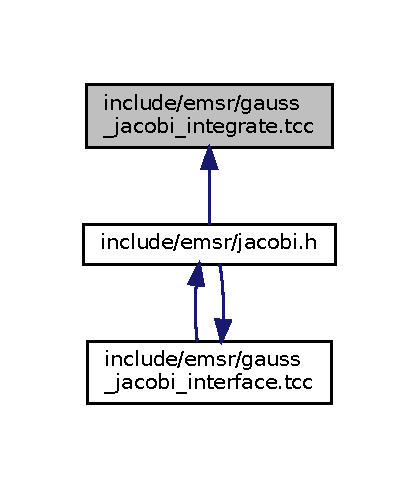
\includegraphics[width=201pt]{gauss__jacobi__integrate_8tcc__dep__incl}
\end{center}
\end{figure}
\doxysubsection*{Macros}
\begin{DoxyCompactItemize}
\item 
\#define \mbox{\hyperlink{gauss__jacobi__integrate_8tcc_ae2b6fbcf3efab2e2aa8dbc185a1ab8b8}{GAUSS\+\_\+\+JACOBI\+\_\+\+INTEGRATE\+\_\+\+TCC}}~1
\end{DoxyCompactItemize}
\doxysubsection*{Functions}
\begin{DoxyCompactItemize}
\item 
{\footnotesize template$<$typename Tp $>$ }\\int \mbox{\hyperlink{gauss__jacobi__integrate_8tcc_a9b4defb4fe750d83c39167fe7508e13a}{jacobi\+\_\+deriv\+\_\+array}} (int np, const \mbox{\hyperlink{test__integral_8tcc_a82f489a4943d33943d0b0f781a801283}{Tp}} $\ast$x, \mbox{\hyperlink{test__integral_8tcc_a82f489a4943d33943d0b0f781a801283}{Tp}} $\ast$result\+\_\+array, int n, double a, double b)
\item 
{\footnotesize template$<$typename Tp $>$ }\\int \mbox{\hyperlink{gauss__jacobi__integrate_8tcc_af231cff99147c096acae672bc377dc70}{jacobi\+\_\+value\+\_\+array}} (int np, const \mbox{\hyperlink{test__integral_8tcc_a82f489a4943d33943d0b0f781a801283}{Tp}} $\ast$x, \mbox{\hyperlink{test__integral_8tcc_a82f489a4943d33943d0b0f781a801283}{Tp}} $\ast$result\+\_\+array, int n, \mbox{\hyperlink{test__integral_8tcc_a82f489a4943d33943d0b0f781a801283}{Tp}} a, \mbox{\hyperlink{test__integral_8tcc_a82f489a4943d33943d0b0f781a801283}{Tp}} b)
\end{DoxyCompactItemize}
\doxysubsection*{Variables}
\begin{DoxyCompactItemize}
\item 
{\footnotesize template$<$typename Tp $>$ }\\const \mbox{\hyperlink{test__integral_8tcc_a82f489a4943d33943d0b0f781a801283}{Tp}} \mbox{\hyperlink{gauss__jacobi__integrate_8tcc_a5cabb6df33c09087e4d207e86b412b56}{EPS}} = \mbox{\hyperlink{test__integral_8tcc_a82f489a4943d33943d0b0f781a801283}{Tp}}(300) $\ast$ std\+::numeric\+\_\+limits$<$\mbox{\hyperlink{test__integral_8tcc_a82f489a4943d33943d0b0f781a801283}{Tp}}$>$\+::epsilon()
\begin{DoxyCompactList}\small\item\em Admissible convergence error. \end{DoxyCompactList}\end{DoxyCompactItemize}


\doxysubsection{Macro Definition Documentation}
\mbox{\Hypertarget{gauss__jacobi__integrate_8tcc_ae2b6fbcf3efab2e2aa8dbc185a1ab8b8}\label{gauss__jacobi__integrate_8tcc_ae2b6fbcf3efab2e2aa8dbc185a1ab8b8}} 
\index{gauss\_jacobi\_integrate.tcc@{gauss\_jacobi\_integrate.tcc}!GAUSS\_JACOBI\_INTEGRATE\_TCC@{GAUSS\_JACOBI\_INTEGRATE\_TCC}}
\index{GAUSS\_JACOBI\_INTEGRATE\_TCC@{GAUSS\_JACOBI\_INTEGRATE\_TCC}!gauss\_jacobi\_integrate.tcc@{gauss\_jacobi\_integrate.tcc}}
\doxysubsubsection{\texorpdfstring{GAUSS\_JACOBI\_INTEGRATE\_TCC}{GAUSS\_JACOBI\_INTEGRATE\_TCC}}
{\footnotesize\ttfamily \#define GAUSS\+\_\+\+JACOBI\+\_\+\+INTEGRATE\+\_\+\+TCC~1}



Definition at line 21 of file gauss\+\_\+jacobi\+\_\+integrate.\+tcc.



\doxysubsection{Function Documentation}
\mbox{\Hypertarget{gauss__jacobi__integrate_8tcc_a9b4defb4fe750d83c39167fe7508e13a}\label{gauss__jacobi__integrate_8tcc_a9b4defb4fe750d83c39167fe7508e13a}} 
\index{gauss\_jacobi\_integrate.tcc@{gauss\_jacobi\_integrate.tcc}!jacobi\_deriv\_array@{jacobi\_deriv\_array}}
\index{jacobi\_deriv\_array@{jacobi\_deriv\_array}!gauss\_jacobi\_integrate.tcc@{gauss\_jacobi\_integrate.tcc}}
\doxysubsubsection{\texorpdfstring{jacobi\_deriv\_array()}{jacobi\_deriv\_array()}}
{\footnotesize\ttfamily template$<$typename Tp $>$ \\
int jacobi\+\_\+deriv\+\_\+array (\begin{DoxyParamCaption}\item[{int}]{np,  }\item[{const \mbox{\hyperlink{test__integral_8tcc_a82f489a4943d33943d0b0f781a801283}{Tp}} $\ast$}]{x,  }\item[{\mbox{\hyperlink{test__integral_8tcc_a82f489a4943d33943d0b0f781a801283}{Tp}} $\ast$}]{result\+\_\+array,  }\item[{int}]{n,  }\item[{double}]{a,  }\item[{double}]{b }\end{DoxyParamCaption})}

Calculates the derivative of the nth order Jacobi polynomial at an array of np points given by the vector x. This function needs two workspaces of size np to do its calculation. If the first one (ws1) is NULL, the function will allocate the necessary memory (using malloc) to do the calculation


\begin{DoxyParams}{Parameters}
{\em np} & Number of points where the polynomial will be calculated \\
\hline
{\em x} & A vector of length np containing the points where the polynomials should be calculated. $-1\le x_i \le 1$. \\
\hline
{\em n} & Order of the Jacobi polynomial whose derivative should be calculated \\
\hline
{\em result\+\_\+array} & An array of length np where the result will be stored \\
\hline
{\em a} & $\alpha$ parameter of Jacobi polynomial \\
\hline
{\em b} & $\beta$ parameter of Jacobi polynomial \\
\hline
{\em ws} & A pointer to a block of memory 2$\ast$np doubles long to be used as workspace. If it is NULL, memory will be allocated using malloc and released at the end \\
\hline
\end{DoxyParams}
\begin{DoxyReturn}{Returns}
Error code defined in gsl\+\_\+errno.\+h or GSL\+\_\+\+SUCCESS if everything was fine 
\end{DoxyReturn}


Definition at line 116 of file gauss\+\_\+jacobi\+\_\+integrate.\+tcc.


\begin{DoxyCode}{0}
\DoxyCodeLine{118   \{}
\DoxyCodeLine{119     \textcolor{keywordtype}{int} code = \mbox{\hyperlink{gauss__jacobi__integrate_8tcc_af231cff99147c096acae672bc377dc70}{jacobi\_value\_array}}(np, x, result\_array,}
\DoxyCodeLine{120                                   n -\/ 1, a + \mbox{\hyperlink{test__integral_8tcc_a82f489a4943d33943d0b0f781a801283}{Tp}}\{1\}, b + \mbox{\hyperlink{test__integral_8tcc_a82f489a4943d33943d0b0f781a801283}{Tp}}\{1\});}
\DoxyCodeLine{121     \textcolor{keywordflow}{if} (code)}
\DoxyCodeLine{122       \textcolor{keywordflow}{return} code;}
\DoxyCodeLine{123     }
\DoxyCodeLine{124     \textcolor{keywordflow}{for} (\textcolor{keywordtype}{int} i = 0; i < np; ++i)}
\DoxyCodeLine{125       result\_array[i] *= 0.5 * (a + b + n + \mbox{\hyperlink{test__integral_8tcc_a82f489a4943d33943d0b0f781a801283}{Tp}}\{1\});}
\DoxyCodeLine{126 }
\DoxyCodeLine{127     \textcolor{keywordflow}{return} code;}
\DoxyCodeLine{128   \}}

\end{DoxyCode}


References jacobi\+\_\+value\+\_\+array(), and Tp.

\mbox{\Hypertarget{gauss__jacobi__integrate_8tcc_af231cff99147c096acae672bc377dc70}\label{gauss__jacobi__integrate_8tcc_af231cff99147c096acae672bc377dc70}} 
\index{gauss\_jacobi\_integrate.tcc@{gauss\_jacobi\_integrate.tcc}!jacobi\_value\_array@{jacobi\_value\_array}}
\index{jacobi\_value\_array@{jacobi\_value\_array}!gauss\_jacobi\_integrate.tcc@{gauss\_jacobi\_integrate.tcc}}
\doxysubsubsection{\texorpdfstring{jacobi\_value\_array()}{jacobi\_value\_array()}}
{\footnotesize\ttfamily template$<$typename Tp $>$ \\
int jacobi\+\_\+value\+\_\+array (\begin{DoxyParamCaption}\item[{int}]{np,  }\item[{const \mbox{\hyperlink{test__integral_8tcc_a82f489a4943d33943d0b0f781a801283}{Tp}} $\ast$}]{x,  }\item[{\mbox{\hyperlink{test__integral_8tcc_a82f489a4943d33943d0b0f781a801283}{Tp}} $\ast$}]{result\+\_\+array,  }\item[{int}]{n,  }\item[{\mbox{\hyperlink{test__integral_8tcc_a82f489a4943d33943d0b0f781a801283}{Tp}}}]{a,  }\item[{\mbox{\hyperlink{test__integral_8tcc_a82f489a4943d33943d0b0f781a801283}{Tp}}}]{b }\end{DoxyParamCaption})}



Definition at line 60 of file gauss\+\_\+jacobi\+\_\+integrate.\+tcc.


\begin{DoxyCode}{0}
\DoxyCodeLine{62   \{}
\DoxyCodeLine{63     \textcolor{keywordflow}{if} (n == 0)}
\DoxyCodeLine{64       \{}
\DoxyCodeLine{65         \textcolor{keywordflow}{for}(\textcolor{keywordtype}{int} i = 0; i < np; ++i)}
\DoxyCodeLine{66           result\_array[i] = \mbox{\hyperlink{test__integral_8tcc_a82f489a4943d33943d0b0f781a801283}{Tp}}\{1\};}
\DoxyCodeLine{67         \textcolor{keywordflow}{return} 0;}
\DoxyCodeLine{68       \}}
\DoxyCodeLine{69 }
\DoxyCodeLine{70     \textcolor{keywordflow}{if} (n == 1)}
\DoxyCodeLine{71       \{}
\DoxyCodeLine{72         \textcolor{keywordflow}{for} (\textcolor{keywordtype}{int} i = 0; i < np; ++i)}
\DoxyCodeLine{73           result\_array[i] = 0.5 * (a -\/ b + (a + b + \mbox{\hyperlink{test__integral_8tcc_a82f489a4943d33943d0b0f781a801283}{Tp}}\{2\}) * x[i]);}
\DoxyCodeLine{74         \textcolor{keywordflow}{return} 0;}
\DoxyCodeLine{75       \}}
\DoxyCodeLine{76 }
\DoxyCodeLine{77     \textcolor{comment}{// General case,}}
\DoxyCodeLine{78     std::vector<Tp> pnm1(np), pnm2(np, \mbox{\hyperlink{test__integral_8tcc_a82f489a4943d33943d0b0f781a801283}{Tp}}\{1\});}
\DoxyCodeLine{79     \textcolor{keywordflow}{for} (\textcolor{keywordtype}{int} i = 0; i < np; ++i)}
\DoxyCodeLine{80       pnm1[i] = 0.5 * (a -\/ b + (a + b + \mbox{\hyperlink{test__integral_8tcc_a82f489a4943d33943d0b0f781a801283}{Tp}}\{2\}) * x[i]);}
\DoxyCodeLine{81 }
\DoxyCodeLine{82     \textcolor{comment}{// Start iterating:}}
\DoxyCodeLine{83     \textcolor{keywordflow}{for} (\textcolor{keywordtype}{int} k = 1; k < n; ++k)}
\DoxyCodeLine{84       \{}
\DoxyCodeLine{85         \textcolor{keyword}{auto} a1 = \mbox{\hyperlink{test__integral_8tcc_a82f489a4943d33943d0b0f781a801283}{Tp}}\{2\} * (k + \mbox{\hyperlink{test__integral_8tcc_a82f489a4943d33943d0b0f781a801283}{Tp}}\{1\}) * (k + a + b + \mbox{\hyperlink{test__integral_8tcc_a82f489a4943d33943d0b0f781a801283}{Tp}}\{1\}) * (\mbox{\hyperlink{test__integral_8tcc_a82f489a4943d33943d0b0f781a801283}{Tp}}\{2\} * k + a + b);}
\DoxyCodeLine{86         \textcolor{keyword}{auto} a2 = (\mbox{\hyperlink{test__integral_8tcc_a82f489a4943d33943d0b0f781a801283}{Tp}}\{2\} * k + a + b + \mbox{\hyperlink{test__integral_8tcc_a82f489a4943d33943d0b0f781a801283}{Tp}}\{1\}) * (a * a -\/ b * b) / a1;}
\DoxyCodeLine{87         \textcolor{keyword}{auto} a3 = (\mbox{\hyperlink{test__integral_8tcc_a82f489a4943d33943d0b0f781a801283}{Tp}}\{2\} * k + a + b) * (\mbox{\hyperlink{test__integral_8tcc_a82f489a4943d33943d0b0f781a801283}{Tp}}\{2\} * k + a + b + \mbox{\hyperlink{test__integral_8tcc_a82f489a4943d33943d0b0f781a801283}{Tp}}\{1\}) * (\mbox{\hyperlink{test__integral_8tcc_a82f489a4943d33943d0b0f781a801283}{Tp}}\{2\} * k + a + b + \mbox{\hyperlink{test__integral_8tcc_a82f489a4943d33943d0b0f781a801283}{Tp}}\{2\}) / a1;}
\DoxyCodeLine{88         \textcolor{keyword}{auto} a4 = \mbox{\hyperlink{test__integral_8tcc_a82f489a4943d33943d0b0f781a801283}{Tp}}\{2\} * (k + a) * (k + b) * (\mbox{\hyperlink{test__integral_8tcc_a82f489a4943d33943d0b0f781a801283}{Tp}}\{2\} * k + a + b + \mbox{\hyperlink{test__integral_8tcc_a82f489a4943d33943d0b0f781a801283}{Tp}}\{2\}) / a1;}
\DoxyCodeLine{89         \textcolor{keywordflow}{for} (\textcolor{keywordtype}{int} i = 0; i < np; ++i)}
\DoxyCodeLine{90           \{}
\DoxyCodeLine{91             result\_array[i] = (a2 + a3 * x[i]) * pnm1[i] -\/ a4 * pnm2[i];}
\DoxyCodeLine{92             pnm2[i] = pnm1[i];}
\DoxyCodeLine{93             pnm1[i] = result\_array[i];}
\DoxyCodeLine{94           \}}
\DoxyCodeLine{95       \}}
\DoxyCodeLine{96 }
\DoxyCodeLine{97     \textcolor{keywordflow}{return} 0;}
\DoxyCodeLine{98   \}}

\end{DoxyCode}


References Tp.



Referenced by jacobi\+\_\+deriv\+\_\+array().



\doxysubsection{Variable Documentation}
\mbox{\Hypertarget{gauss__jacobi__integrate_8tcc_a5cabb6df33c09087e4d207e86b412b56}\label{gauss__jacobi__integrate_8tcc_a5cabb6df33c09087e4d207e86b412b56}} 
\index{gauss\_jacobi\_integrate.tcc@{gauss\_jacobi\_integrate.tcc}!EPS@{EPS}}
\index{EPS@{EPS}!gauss\_jacobi\_integrate.tcc@{gauss\_jacobi\_integrate.tcc}}
\doxysubsubsection{\texorpdfstring{EPS}{EPS}}
{\footnotesize\ttfamily template$<$typename Tp $>$ \\
const \mbox{\hyperlink{test__integral_8tcc_a82f489a4943d33943d0b0f781a801283}{Tp}} EPS = \mbox{\hyperlink{test__integral_8tcc_a82f489a4943d33943d0b0f781a801283}{Tp}}(300) $\ast$ std\+::numeric\+\_\+limits$<$\mbox{\hyperlink{test__integral_8tcc_a82f489a4943d33943d0b0f781a801283}{Tp}}$>$\+::epsilon()}



Admissible convergence error. 



Definition at line 41 of file gauss\+\_\+jacobi\+\_\+integrate.\+tcc.


\hypertarget{gauss__jacobi__interface_8tcc}{}\doxysection{include/emsr/gauss\+\_\+jacobi\+\_\+interface.tcc File Reference}
\label{gauss__jacobi__interface_8tcc}\index{include/emsr/gauss\_jacobi\_interface.tcc@{include/emsr/gauss\_jacobi\_interface.tcc}}
{\ttfamily \#include $<$cstdlib$>$}\newline
{\ttfamily \#include $<$numeric$>$}\newline
{\ttfamily \#include $<$emsr/jacobi.\+h$>$}\newline
{\ttfamily \#include $<$emsr/integration\+\_\+error.\+h$>$}\newline
Include dependency graph for gauss\+\_\+jacobi\+\_\+interface.\+tcc\+:
\nopagebreak
\begin{figure}[H]
\begin{center}
\leavevmode
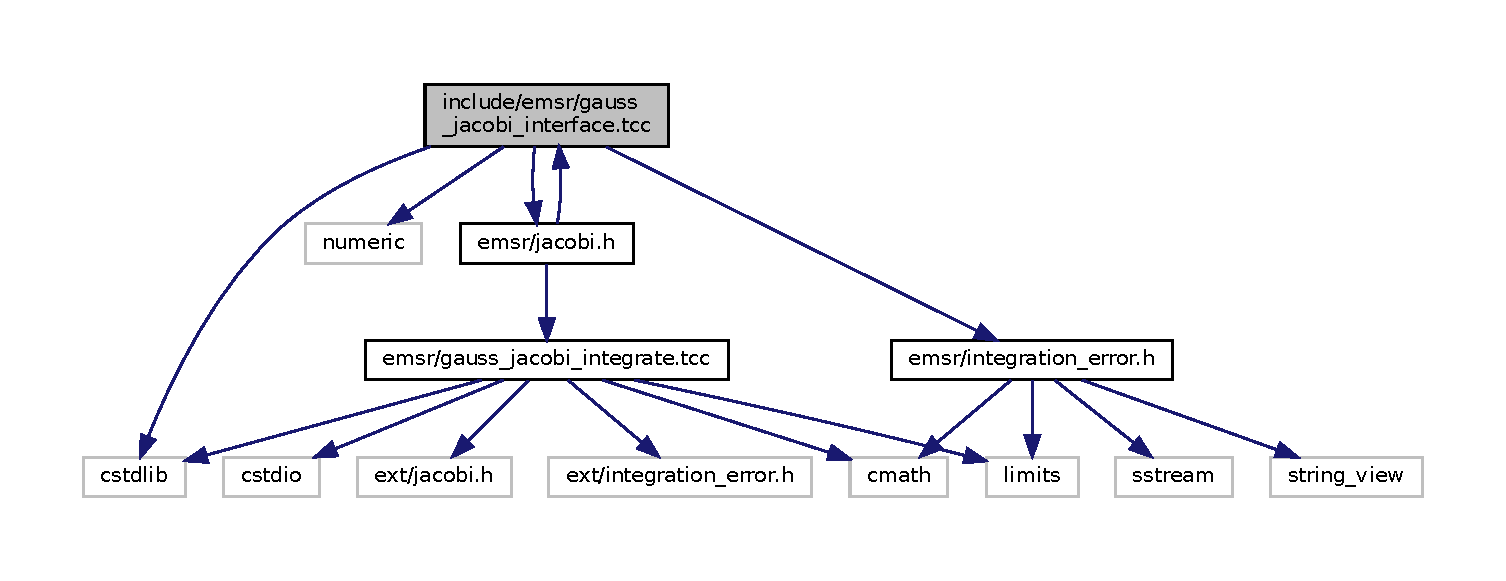
\includegraphics[width=350pt]{gauss__jacobi__interface_8tcc__incl}
\end{center}
\end{figure}
This graph shows which files directly or indirectly include this file\+:
\nopagebreak
\begin{figure}[H]
\begin{center}
\leavevmode
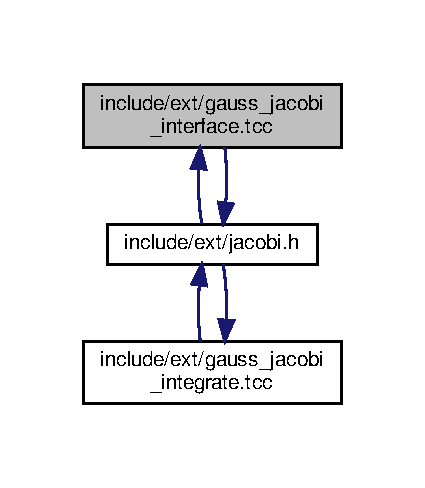
\includegraphics[width=201pt]{gauss__jacobi__interface_8tcc__dep__incl}
\end{center}
\end{figure}
\doxysubsection*{Macros}
\begin{DoxyCompactItemize}
\item 
\#define \mbox{\hyperlink{gauss__jacobi__interface_8tcc_adef683aafaba9ea14e575964a5bdbc8d}{GAUSS\+\_\+\+JACOBI\+\_\+\+INTERFACE\+\_\+\+TCC}}~1
\end{DoxyCompactItemize}
\doxysubsection*{Functions}
\begin{DoxyCompactItemize}
\item 
{\footnotesize template$<$typename Tp $>$ }\\void \mbox{\hyperlink{gauss__jacobi__interface_8tcc_ac0ed91d648c6c895a9ec99cf0e863aaa}{matvec}} (std\+::size\+\_\+t \+\_\+\+\_\+n, const \mbox{\hyperlink{test__integral_8tcc_a82f489a4943d33943d0b0f781a801283}{Tp}} $\ast$\+\_\+\+\_\+A, const \mbox{\hyperlink{test__integral_8tcc_a82f489a4943d33943d0b0f781a801283}{Tp}} $\ast$\+\_\+\+\_\+x, \mbox{\hyperlink{test__integral_8tcc_a82f489a4943d33943d0b0f781a801283}{Tp}} $\ast$\+\_\+\+\_\+y)
\end{DoxyCompactItemize}


\doxysubsection{Macro Definition Documentation}
\mbox{\Hypertarget{gauss__jacobi__interface_8tcc_adef683aafaba9ea14e575964a5bdbc8d}\label{gauss__jacobi__interface_8tcc_adef683aafaba9ea14e575964a5bdbc8d}} 
\index{gauss\_jacobi\_interface.tcc@{gauss\_jacobi\_interface.tcc}!GAUSS\_JACOBI\_INTERFACE\_TCC@{GAUSS\_JACOBI\_INTERFACE\_TCC}}
\index{GAUSS\_JACOBI\_INTERFACE\_TCC@{GAUSS\_JACOBI\_INTERFACE\_TCC}!gauss\_jacobi\_interface.tcc@{gauss\_jacobi\_interface.tcc}}
\doxysubsubsection{\texorpdfstring{GAUSS\_JACOBI\_INTERFACE\_TCC}{GAUSS\_JACOBI\_INTERFACE\_TCC}}
{\footnotesize\ttfamily \#define GAUSS\+\_\+\+JACOBI\+\_\+\+INTERFACE\+\_\+\+TCC~1}



Definition at line 22 of file gauss\+\_\+jacobi\+\_\+interface.\+tcc.



\doxysubsection{Function Documentation}
\mbox{\Hypertarget{gauss__jacobi__interface_8tcc_ac0ed91d648c6c895a9ec99cf0e863aaa}\label{gauss__jacobi__interface_8tcc_ac0ed91d648c6c895a9ec99cf0e863aaa}} 
\index{gauss\_jacobi\_interface.tcc@{gauss\_jacobi\_interface.tcc}!matvec@{matvec}}
\index{matvec@{matvec}!gauss\_jacobi\_interface.tcc@{gauss\_jacobi\_interface.tcc}}
\doxysubsubsection{\texorpdfstring{matvec()}{matvec()}}
{\footnotesize\ttfamily template$<$typename Tp $>$ \\
void matvec (\begin{DoxyParamCaption}\item[{std\+::size\+\_\+t}]{\+\_\+\+\_\+n,  }\item[{const \mbox{\hyperlink{test__integral_8tcc_a82f489a4943d33943d0b0f781a801283}{Tp}} $\ast$}]{\+\_\+\+\_\+A,  }\item[{const \mbox{\hyperlink{test__integral_8tcc_a82f489a4943d33943d0b0f781a801283}{Tp}} $\ast$}]{\+\_\+\+\_\+x,  }\item[{\mbox{\hyperlink{test__integral_8tcc_a82f489a4943d33943d0b0f781a801283}{Tp}} $\ast$}]{\+\_\+\+\_\+y }\end{DoxyParamCaption})}



Definition at line 84 of file gauss\+\_\+jacobi\+\_\+interface.\+tcc.


\begin{DoxyCode}{0}
\DoxyCodeLine{85   \{}
\DoxyCodeLine{86     \textcolor{keywordflow}{for} (std::size\_t \_\_ir = 0; \_\_ir < \_\_n; ++\_\_ir)}
\DoxyCodeLine{87       \{}
\DoxyCodeLine{88         \_\_y[\_\_ir] = \mbox{\hyperlink{test__integral_8tcc_a82f489a4943d33943d0b0f781a801283}{Tp}}\{0\};}
\DoxyCodeLine{89         \textcolor{keywordflow}{for} (std::size\_t \_\_ic = 0; \_\_ic < \_\_n; ++\_\_ic)}
\DoxyCodeLine{90           \_\_y[\_\_ir] += \_\_A[\_\_ir][\_\_ic] * \_\_x[\_\_ic];}
\DoxyCodeLine{91       \}}
\DoxyCodeLine{92   \}}

\end{DoxyCode}


References Tp.


\hypertarget{gauss__kronrod__integral_8tcc}{}\doxysection{include/emsr/gauss\+\_\+kronrod\+\_\+integral.tcc File Reference}
\label{gauss__kronrod__integral_8tcc}\index{include/emsr/gauss\_kronrod\_integral.tcc@{include/emsr/gauss\_kronrod\_integral.tcc}}
{\ttfamily \#include $<$type\+\_\+traits$>$}\newline
{\ttfamily \#include $<$vector$>$}\newline
{\ttfamily \#include $<$cmath$>$}\newline
{\ttfamily \#include $<$array$>$}\newline
{\ttfamily \#include $<$stdexcept$>$}\newline
{\ttfamily \#include $<$emsr/integration\+\_\+error.\+h$>$}\newline
{\ttfamily \#include $<$emsr/gauss\+\_\+kronrod\+\_\+rule.\+tcc$>$}\newline
Include dependency graph for gauss\+\_\+kronrod\+\_\+integral.\+tcc\+:
\nopagebreak
\begin{figure}[H]
\begin{center}
\leavevmode
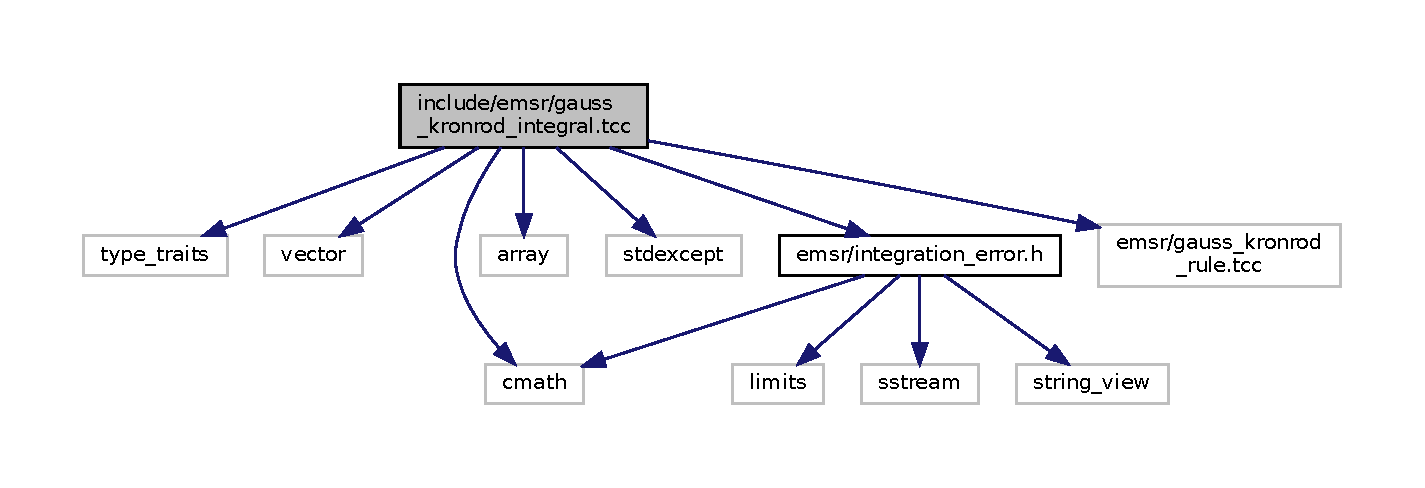
\includegraphics[width=350pt]{gauss__kronrod__integral_8tcc__incl}
\end{center}
\end{figure}
This graph shows which files directly or indirectly include this file\+:
\nopagebreak
\begin{figure}[H]
\begin{center}
\leavevmode
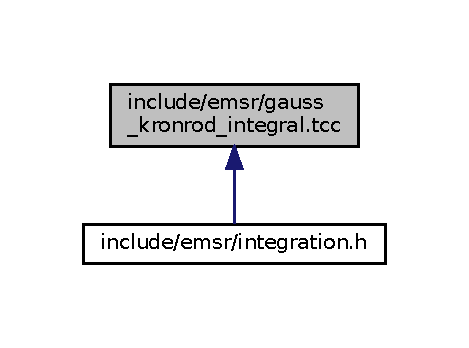
\includegraphics[width=225pt]{gauss__kronrod__integral_8tcc__dep__incl}
\end{center}
\end{figure}
\doxysubsection*{Classes}
\begin{DoxyCompactItemize}
\item 
struct \mbox{\hyperlink{structemsr_1_1qk__integrator_3_01Tp_00_01FuncTp_00_01Kronrod__15_01_4}{emsr\+::qk\+\_\+integrator$<$ Tp, Func\+Tp, Kronrod\+\_\+15 $>$}}
\item 
struct \mbox{\hyperlink{structemsr_1_1qk__integrator_3_01Tp_00_01FuncTp_00_01Kronrod__21_01_4}{emsr\+::qk\+\_\+integrator$<$ Tp, Func\+Tp, Kronrod\+\_\+21 $>$}}
\item 
struct \mbox{\hyperlink{structemsr_1_1qk__integrator_3_01Tp_00_01FuncTp_00_01Kronrod__31_01_4}{emsr\+::qk\+\_\+integrator$<$ Tp, Func\+Tp, Kronrod\+\_\+31 $>$}}
\item 
struct \mbox{\hyperlink{structemsr_1_1qk__integrator_3_01Tp_00_01FuncTp_00_01Kronrod__41_01_4}{emsr\+::qk\+\_\+integrator$<$ Tp, Func\+Tp, Kronrod\+\_\+41 $>$}}
\item 
struct \mbox{\hyperlink{structemsr_1_1qk__integrator_3_01Tp_00_01FuncTp_00_01Kronrod__51_01_4}{emsr\+::qk\+\_\+integrator$<$ Tp, Func\+Tp, Kronrod\+\_\+51 $>$}}
\item 
struct \mbox{\hyperlink{structemsr_1_1qk__integrator_3_01Tp_00_01FuncTp_00_01Kronrod__61_01_4}{emsr\+::qk\+\_\+integrator$<$ Tp, Func\+Tp, Kronrod\+\_\+61 $>$}}
\end{DoxyCompactItemize}
\doxysubsection*{Namespaces}
\begin{DoxyCompactItemize}
\item 
 \mbox{\hyperlink{namespaceemsr}{emsr}}
\end{DoxyCompactItemize}
\doxysubsection*{Macros}
\begin{DoxyCompactItemize}
\item 
\#define \mbox{\hyperlink{gauss__kronrod__integral_8tcc_aa9eb111a71ca7ff9b6e4a1136a08c8a2}{GAUSS\+\_\+\+KRONROD\+\_\+\+INTERGAL\+\_\+\+TCC}}~1
\end{DoxyCompactItemize}
\doxysubsection*{Functions}
\begin{DoxyCompactItemize}
\item 
{\footnotesize template$<$typename Tp , typename Func\+Tp $>$ }\\auto \mbox{\hyperlink{namespaceemsr_a8aa9c40640a93a4ee705ec956a75f26a}{emsr\+::qk\+\_\+integrate}} (Func\+Tp func, \mbox{\hyperlink{test__integral_8tcc_a82f489a4943d33943d0b0f781a801283}{Tp}} lower, \mbox{\hyperlink{test__integral_8tcc_a82f489a4943d33943d0b0f781a801283}{Tp}} upper, Kronrod\+\_\+\+Rule qkintrule) -\/$>$ gauss\+\_\+kronrod\+\_\+integral\+\_\+t$<$ \mbox{\hyperlink{test__integral_8tcc_a82f489a4943d33943d0b0f781a801283}{Tp}}, std\+::invoke\+\_\+result\+\_\+t$<$ Func\+Tp, \mbox{\hyperlink{test__integral_8tcc_a82f489a4943d33943d0b0f781a801283}{Tp}} $>$$>$
\item 
{\footnotesize template$<$typename Area\+Tp , typename Abs\+Area\+Tp $>$ }\\bool \mbox{\hyperlink{namespaceemsr_a56629b4d7a6ed0197866d22291f2a17e}{emsr\+::test\+\_\+positivity}} (Area\+Tp result, Abs\+Area\+Tp resabs)
\end{DoxyCompactItemize}


\doxysubsection{Macro Definition Documentation}
\mbox{\Hypertarget{gauss__kronrod__integral_8tcc_aa9eb111a71ca7ff9b6e4a1136a08c8a2}\label{gauss__kronrod__integral_8tcc_aa9eb111a71ca7ff9b6e4a1136a08c8a2}} 
\index{gauss\_kronrod\_integral.tcc@{gauss\_kronrod\_integral.tcc}!GAUSS\_KRONROD\_INTERGAL\_TCC@{GAUSS\_KRONROD\_INTERGAL\_TCC}}
\index{GAUSS\_KRONROD\_INTERGAL\_TCC@{GAUSS\_KRONROD\_INTERGAL\_TCC}!gauss\_kronrod\_integral.tcc@{gauss\_kronrod\_integral.tcc}}
\doxysubsubsection{\texorpdfstring{GAUSS\_KRONROD\_INTERGAL\_TCC}{GAUSS\_KRONROD\_INTERGAL\_TCC}}
{\footnotesize\ttfamily \#define GAUSS\+\_\+\+KRONROD\+\_\+\+INTERGAL\+\_\+\+TCC~1}



Definition at line 26 of file gauss\+\_\+kronrod\+\_\+integral.\+tcc.


\hypertarget{gauss__laguerre__integrate_8h}{}\doxysection{include/emsr/gauss\+\_\+laguerre\+\_\+integrate.h File Reference}
\label{gauss__laguerre__integrate_8h}\index{include/emsr/gauss\_laguerre\_integrate.h@{include/emsr/gauss\_laguerre\_integrate.h}}
{\ttfamily \#include $<$stdexcept$>$}\newline
{\ttfamily \#include $<$type\+\_\+traits$>$}\newline
{\ttfamily \#include $<$vector$>$}\newline
{\ttfamily \#include $<$emsr/quadrature\+\_\+point.\+h$>$}\newline
Include dependency graph for gauss\+\_\+laguerre\+\_\+integrate.\+h\+:
\nopagebreak
\begin{figure}[H]
\begin{center}
\leavevmode
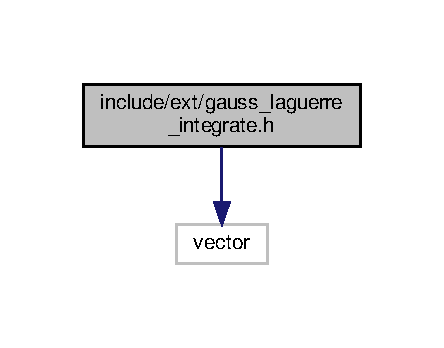
\includegraphics[width=350pt]{gauss__laguerre__integrate_8h__incl}
\end{center}
\end{figure}
\doxysubsection*{Namespaces}
\begin{DoxyCompactItemize}
\item 
 \mbox{\hyperlink{namespaceemsr}{emsr}}
\end{DoxyCompactItemize}
\doxysubsection*{Variables}
\begin{DoxyCompactItemize}
\item 
{\footnotesize template$<$typename Tp , typename Func $>$ }\\decltype(std\+::invoke\+\_\+result\+\_\+t$<$ Func, \mbox{\hyperlink{test__integral_8tcc_a82f489a4943d33943d0b0f781a801283}{Tp}} $>$\{\} $\ast$\mbox{\hyperlink{test__integral_8tcc_a82f489a4943d33943d0b0f781a801283}{Tp}}\{\} \mbox{\hyperlink{namespaceemsr_a0e461ebebd31989d720f0028fca3761a}{emsr\+::gauss\+\_\+laguerre\+\_\+integrate}} )(Func func, unsigned int n, \mbox{\hyperlink{test__integral_8tcc_a82f489a4943d33943d0b0f781a801283}{Tp}} alpha)
\end{DoxyCompactItemize}

\hypertarget{gauss__legendre__table_8h}{}\doxysection{include/emsr/gauss\+\_\+legendre\+\_\+table.h File Reference}
\label{gauss__legendre__table_8h}\index{include/emsr/gauss\_legendre\_table.h@{include/emsr/gauss\_legendre\_table.h}}
{\ttfamily \#include $<$cmath$>$}\newline
{\ttfamily \#include $<$emsr/gauss\+\_\+legendre\+\_\+table.\+tcc$>$}\newline
Include dependency graph for gauss\+\_\+legendre\+\_\+table.\+h\+:
\nopagebreak
\begin{figure}[H]
\begin{center}
\leavevmode
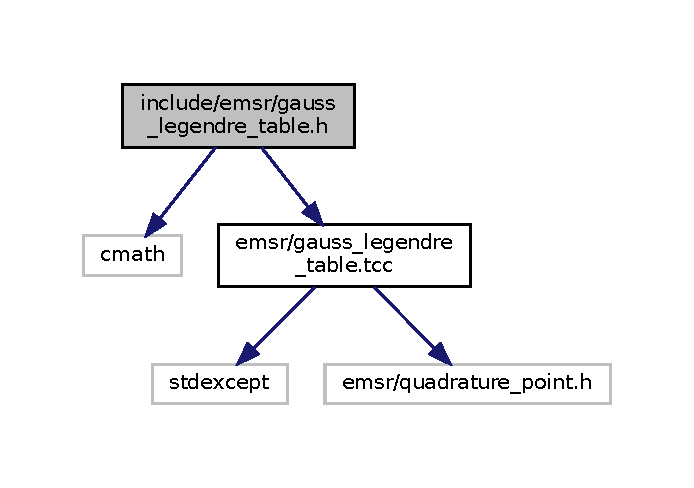
\includegraphics[width=274pt]{gauss__legendre__table_8h__incl}
\end{center}
\end{figure}
This graph shows which files directly or indirectly include this file\+:
\nopagebreak
\begin{figure}[H]
\begin{center}
\leavevmode
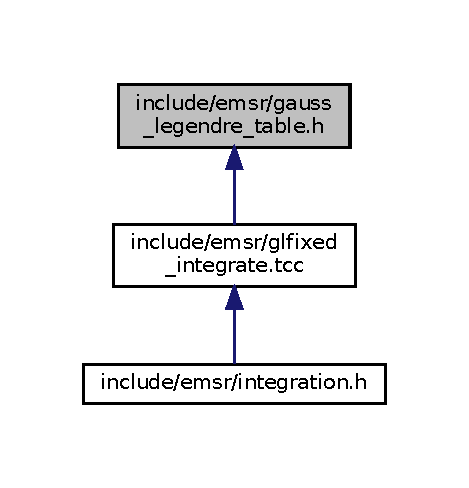
\includegraphics[width=225pt]{gauss__legendre__table_8h__dep__incl}
\end{center}
\end{figure}
\doxysubsection*{Classes}
\begin{DoxyCompactItemize}
\item 
struct \mbox{\hyperlink{structemsr_1_1gauss__legendre__table}{emsr\+::gauss\+\_\+legendre\+\_\+table$<$ Tp $>$}}
\end{DoxyCompactItemize}
\doxysubsection*{Namespaces}
\begin{DoxyCompactItemize}
\item 
 \mbox{\hyperlink{namespaceemsr}{emsr}}
\end{DoxyCompactItemize}
\doxysubsection*{Enumerations}
\begin{DoxyCompactItemize}
\item 
enum \mbox{\hyperlink{namespaceemsr_adf254122bd11c3c2304ffe11f55d33f9}{emsr\+::\+Gauss\+\_\+\+Legendre\+\_\+\+Rule}} \{ \newline
\mbox{\hyperlink{namespaceemsr_adf254122bd11c3c2304ffe11f55d33f9aa4206cd1bd3a20c14137a61785e60c54}{emsr\+::\+GL\+\_\+2}} = 2
, \mbox{\hyperlink{namespaceemsr_adf254122bd11c3c2304ffe11f55d33f9a2cf8bba29976660d4831d2cfc4c4f88c}{emsr\+::\+GL\+\_\+4}} = 4
, \mbox{\hyperlink{namespaceemsr_adf254122bd11c3c2304ffe11f55d33f9a993a1b502c4b67eccc67275246fcc449}{emsr\+::\+GL\+\_\+6}} = 6
, \mbox{\hyperlink{namespaceemsr_adf254122bd11c3c2304ffe11f55d33f9a75708bbf0e774225fe10a498cab55d57}{emsr\+::\+GL\+\_\+8}} = 8
, \newline
\mbox{\hyperlink{namespaceemsr_adf254122bd11c3c2304ffe11f55d33f9a337c8bb034fa5515363bf89654ed2437}{emsr\+::\+GL\+\_\+10}} = 10
, \mbox{\hyperlink{namespaceemsr_adf254122bd11c3c2304ffe11f55d33f9aedfc3b5492d777796e03d9c79c303f48}{emsr\+::\+GL\+\_\+12}} = 12
, \mbox{\hyperlink{namespaceemsr_adf254122bd11c3c2304ffe11f55d33f9ab70111671e5ab8933b102edf1522afe0}{emsr\+::\+GL\+\_\+14}} = 14
, \mbox{\hyperlink{namespaceemsr_adf254122bd11c3c2304ffe11f55d33f9abfd841ed687edd18a1ff22d9b6677fbf}{emsr\+::\+GL\+\_\+16}} = 16
, \newline
\mbox{\hyperlink{namespaceemsr_adf254122bd11c3c2304ffe11f55d33f9ad1f40274a6fdadbba7e2deeed6740440}{emsr\+::\+GL\+\_\+18}} = 18
, \mbox{\hyperlink{namespaceemsr_adf254122bd11c3c2304ffe11f55d33f9aa66ca24e75fd11f8ab9a72f63f4d8b55}{emsr\+::\+GL\+\_\+20}} = 20
, \mbox{\hyperlink{namespaceemsr_adf254122bd11c3c2304ffe11f55d33f9a95863715ac03c6636fda0c74bdbb1613}{emsr\+::\+GL\+\_\+32}} = 32
, \mbox{\hyperlink{namespaceemsr_adf254122bd11c3c2304ffe11f55d33f9abb8d37b6e065b593a35d11f4071a34ff}{emsr\+::\+GL\+\_\+64}} = 64
, \newline
\mbox{\hyperlink{namespaceemsr_adf254122bd11c3c2304ffe11f55d33f9a2c2635549966aa44b2b37a9d9511e07d}{emsr\+::\+GL\+\_\+96}} = 96
, \mbox{\hyperlink{namespaceemsr_adf254122bd11c3c2304ffe11f55d33f9abaff71fd9f46458318f88ab42cfb6749}{emsr\+::\+GL\+\_\+100}} = 100
, \mbox{\hyperlink{namespaceemsr_adf254122bd11c3c2304ffe11f55d33f9a0783e95e7b5a44e47ec3608d270a9746}{emsr\+::\+GL\+\_\+128}} = 128
, \mbox{\hyperlink{namespaceemsr_adf254122bd11c3c2304ffe11f55d33f9aca85670d03157742028a86b9be1416ac}{emsr\+::\+GL\+\_\+256}} = 256
, \newline
\mbox{\hyperlink{namespaceemsr_adf254122bd11c3c2304ffe11f55d33f9a8e8a2f6ce8afdf1874d5e252657b3f94}{emsr\+::\+GL\+\_\+512}} = 512
, \mbox{\hyperlink{namespaceemsr_adf254122bd11c3c2304ffe11f55d33f9afe625b5558867d22a101a3c3db40de88}{emsr\+::\+GL\+\_\+1024}} = 1024
, \mbox{\hyperlink{namespaceemsr_adf254122bd11c3c2304ffe11f55d33f9ae548c81a5ce7a3f5a59c35fd48be8573}{emsr\+::\+GL\+\_\+3}} = 3
, \mbox{\hyperlink{namespaceemsr_adf254122bd11c3c2304ffe11f55d33f9a35e85fc6b730189248d445c0a4b5de8c}{emsr\+::\+GL\+\_\+5}} = 5
, \newline
\mbox{\hyperlink{namespaceemsr_adf254122bd11c3c2304ffe11f55d33f9a16321464e958b7a24df841e7cb5c4daa}{emsr\+::\+GL\+\_\+7}} = 7
, \mbox{\hyperlink{namespaceemsr_adf254122bd11c3c2304ffe11f55d33f9a2068ad29824b165426321c76876b2d38}{emsr\+::\+GL\+\_\+9}} = 9
, \mbox{\hyperlink{namespaceemsr_adf254122bd11c3c2304ffe11f55d33f9a866fce702d4c1fe3a81ebfb22c18444b}{emsr\+::\+GL\+\_\+11}} = 11
, \mbox{\hyperlink{namespaceemsr_adf254122bd11c3c2304ffe11f55d33f9a33082fa9aac7cf3b1217ba91f0e53f1e}{emsr\+::\+GL\+\_\+13}} = 13
, \newline
\mbox{\hyperlink{namespaceemsr_adf254122bd11c3c2304ffe11f55d33f9a00326791ed99fa3e4f5cd75f2370b5d0}{emsr\+::\+GL\+\_\+15}} = 15
, \mbox{\hyperlink{namespaceemsr_adf254122bd11c3c2304ffe11f55d33f9a6bd93507e774138c7471c921e65feba0}{emsr\+::\+GL\+\_\+17}} = 17
, \mbox{\hyperlink{namespaceemsr_adf254122bd11c3c2304ffe11f55d33f9a61f6d75b2c06ffec653beece63f1dcdb}{emsr\+::\+GL\+\_\+19}} = 19
 \}
\end{DoxyCompactItemize}
\doxysubsection*{Variables}
\begin{DoxyCompactItemize}
\item 
const gauss\+\_\+legendre\+\_\+table$<$ long double $>$ \mbox{\hyperlink{namespaceemsr_aca7ebd8e66e48cb5d513e91beafeb56e}{emsr\+::gauss\+\_\+legendre\+\_\+precomp}} \mbox{[}$\,$\mbox{]}
\item 
const std\+::size\+\_\+t \mbox{\hyperlink{namespaceemsr_a9a28ddfdeabb3b352fddf4d2d5b21788}{emsr\+::num\+\_\+gauss\+\_\+legendre\+\_\+precomp}}
\item 
constexpr long double \mbox{\hyperlink{namespaceemsr_a1c9967ef9f3760a5f05019d7dc4708a9}{emsr\+::w10}} \mbox{[}5\mbox{]}
\item 
constexpr long double \mbox{\hyperlink{namespaceemsr_ac8fc2345165e41ad7ef84286c3c3643d}{emsr\+::w100}} \mbox{[}50\mbox{]}
\item 
constexpr long double \mbox{\hyperlink{namespaceemsr_a9e6a5cae36831e895c9ebdab3ecbd79b}{emsr\+::w1024}} \mbox{[}512\mbox{]}
\item 
constexpr long double \mbox{\hyperlink{namespaceemsr_ac60f16e28917fa43d24b79e375e448dc}{emsr\+::w11}} \mbox{[}6\mbox{]}
\item 
constexpr long double \mbox{\hyperlink{namespaceemsr_abda921f44f6a5b76440f3101c54f94f2}{emsr\+::w12}} \mbox{[}6\mbox{]}
\item 
constexpr long double \mbox{\hyperlink{namespaceemsr_a482524b73b830c996d02ffccb30b0f67}{emsr\+::w128}} \mbox{[}64\mbox{]}
\item 
constexpr long double \mbox{\hyperlink{namespaceemsr_aa564b194a5ebe5f30d3956d72963e0f8}{emsr\+::w13}} \mbox{[}7\mbox{]}
\item 
constexpr long double \mbox{\hyperlink{namespaceemsr_a79ee7432f0d7ee303c973937d0e55424}{emsr\+::w14}} \mbox{[}7\mbox{]}
\item 
constexpr long double \mbox{\hyperlink{namespaceemsr_a601fcae77bc636012f75ccb4923d79b4}{emsr\+::w15}} \mbox{[}8\mbox{]}
\item 
constexpr long double \mbox{\hyperlink{namespaceemsr_af79cb46e2d6e1df6dd4fe72427044e37}{emsr\+::w16}} \mbox{[}8\mbox{]}
\item 
constexpr long double \mbox{\hyperlink{namespaceemsr_a5eea03d51f6d7ad20380f1144c27eeb4}{emsr\+::w17}} \mbox{[}9\mbox{]}
\item 
constexpr long double \mbox{\hyperlink{namespaceemsr_ade12cc70f905a22cecdcb92caef75a71}{emsr\+::w18}} \mbox{[}9\mbox{]}
\item 
constexpr long double \mbox{\hyperlink{namespaceemsr_a1a3d9285b7b26c901074d777aae7086a}{emsr\+::w19}} \mbox{[}10\mbox{]}
\item 
constexpr long double \mbox{\hyperlink{namespaceemsr_a6add711d5836cece5d03f91a798246c6}{emsr\+::w2}} \mbox{[}1\mbox{]}
\item 
constexpr long double \mbox{\hyperlink{namespaceemsr_a6e7a5adbe405e9bd77c31dd3d902794a}{emsr\+::w20}} \mbox{[}10\mbox{]}
\item 
constexpr long double \mbox{\hyperlink{namespaceemsr_a401000e92406f605f47588e0bb4cd301}{emsr\+::w256}} \mbox{[}128\mbox{]}
\item 
constexpr long double \mbox{\hyperlink{namespaceemsr_a91fb80d8204135a7efe7493061b6d883}{emsr\+::w3}} \mbox{[}2\mbox{]}
\item 
constexpr long double \mbox{\hyperlink{namespaceemsr_a1bd252aaa2acba26034d994dcd9565db}{emsr\+::w32}} \mbox{[}16\mbox{]}
\item 
constexpr long double \mbox{\hyperlink{namespaceemsr_a35129f2b04727c8ce41ff99f4f226c05}{emsr\+::w4}} \mbox{[}2\mbox{]}
\item 
constexpr long double \mbox{\hyperlink{namespaceemsr_afd9f4d550a1b66223db265abd4b04056}{emsr\+::w5}} \mbox{[}3\mbox{]}
\item 
constexpr long double \mbox{\hyperlink{namespaceemsr_a567c1670832eba5d3681a047dad9fbc6}{emsr\+::w512}} \mbox{[}256\mbox{]}
\item 
constexpr long double \mbox{\hyperlink{namespaceemsr_a2783902ace058395ab15b3044b2ce785}{emsr\+::w6}} \mbox{[}3\mbox{]}
\item 
constexpr long double \mbox{\hyperlink{namespaceemsr_af59c734070333598298f8e23c4ef3320}{emsr\+::w64}} \mbox{[}32\mbox{]}
\item 
constexpr long double \mbox{\hyperlink{namespaceemsr_a9ee151e870d97ff67ba762d48d638e91}{emsr\+::w7}} \mbox{[}4\mbox{]}
\item 
constexpr long double \mbox{\hyperlink{namespaceemsr_ae66b7e711a6da8a60da3d97fe1e1a282}{emsr\+::w8}} \mbox{[}4\mbox{]}
\item 
constexpr long double \mbox{\hyperlink{namespaceemsr_a79c4cea18daace03607a31a5656dcaa1}{emsr\+::w9}} \mbox{[}5\mbox{]}
\item 
constexpr long double \mbox{\hyperlink{namespaceemsr_a2755a3e4d6e41a763aca529ffa3db443}{emsr\+::w96}} \mbox{[}48\mbox{]}
\item 
constexpr long double \mbox{\hyperlink{namespaceemsr_a9da1de9ba66cba015f19764ff436f528}{emsr\+::x10}} \mbox{[}5\mbox{]}
\item 
constexpr long double \mbox{\hyperlink{namespaceemsr_af913a346379d4f5b1da71dc57f57920e}{emsr\+::x100}} \mbox{[}50\mbox{]}
\item 
constexpr long double \mbox{\hyperlink{namespaceemsr_a0883cf5facadd5e095222677c90ecd72}{emsr\+::x1024}} \mbox{[}512\mbox{]}
\item 
constexpr long double \mbox{\hyperlink{namespaceemsr_a4ce27ac647e9121c55c97e9904b08a02}{emsr\+::x11}} \mbox{[}6\mbox{]}
\item 
constexpr long double \mbox{\hyperlink{namespaceemsr_a4492822f4977f583d30e520d95bf3d82}{emsr\+::x12}} \mbox{[}6\mbox{]}
\item 
constexpr long double \mbox{\hyperlink{namespaceemsr_a69bb64c249fc5557d41a94fa7cba7ade}{emsr\+::x128}} \mbox{[}64\mbox{]}
\item 
constexpr long double \mbox{\hyperlink{namespaceemsr_a26a50389f528980130adb0a414b0655a}{emsr\+::x13}} \mbox{[}7\mbox{]}
\item 
constexpr long double \mbox{\hyperlink{namespaceemsr_a5dfb0ec5ddeb72a0ec89b3c3f067cfc0}{emsr\+::x14}} \mbox{[}7\mbox{]}
\item 
constexpr long double \mbox{\hyperlink{namespaceemsr_ae39a3670f2c237f848924b70bf2f8a21}{emsr\+::x15}} \mbox{[}8\mbox{]}
\item 
constexpr long double \mbox{\hyperlink{namespaceemsr_a5d4dbde783766b8f13beb2b0828130f4}{emsr\+::x16}} \mbox{[}8\mbox{]}
\item 
constexpr long double \mbox{\hyperlink{namespaceemsr_af77b9ecbce3c5af8bfea15962a98aa1e}{emsr\+::x17}} \mbox{[}9\mbox{]}
\item 
constexpr long double \mbox{\hyperlink{namespaceemsr_a5ac8c771679fa5a8a1c0c04f2f95d2de}{emsr\+::x18}} \mbox{[}9\mbox{]}
\item 
constexpr long double \mbox{\hyperlink{namespaceemsr_a553b9a1695178ecb64dfc19ba8c50f56}{emsr\+::x19}} \mbox{[}10\mbox{]}
\item 
constexpr long double \mbox{\hyperlink{namespaceemsr_a28390b2752d6986409a54aff919a6d7c}{emsr\+::x2}} \mbox{[}1\mbox{]}
\item 
constexpr long double \mbox{\hyperlink{namespaceemsr_a70f398d4c6b4f4578f4438c320e4a3e8}{emsr\+::x20}} \mbox{[}10\mbox{]}
\item 
constexpr long double \mbox{\hyperlink{namespaceemsr_ab4bc36970b840649accbbc0884c51f95}{emsr\+::x256}} \mbox{[}128\mbox{]}
\item 
constexpr long double \mbox{\hyperlink{namespaceemsr_a814f168b3f4e5677a82859c73c865644}{emsr\+::x3}} \mbox{[}2\mbox{]}
\item 
constexpr long double \mbox{\hyperlink{namespaceemsr_aef3d01dcc3f74889b0381ed0762f6b30}{emsr\+::x32}} \mbox{[}16\mbox{]}
\item 
constexpr long double \mbox{\hyperlink{namespaceemsr_a0d0bfdb7309e6712924a4f6a54e34b69}{emsr\+::x4}} \mbox{[}2\mbox{]}
\item 
constexpr long double \mbox{\hyperlink{namespaceemsr_ae352e1c812605c1f48086f8d83139ec0}{emsr\+::x5}} \mbox{[}3\mbox{]}
\item 
constexpr long double \mbox{\hyperlink{namespaceemsr_aa313456fb2a36aaa3313853498e88b46}{emsr\+::x512}} \mbox{[}256\mbox{]}
\item 
constexpr long double \mbox{\hyperlink{namespaceemsr_ac13dd34652f12b8a2aebf6e5028c7216}{emsr\+::x6}} \mbox{[}3\mbox{]}
\item 
constexpr long double \mbox{\hyperlink{namespaceemsr_abebdbffb9a45fbf2f43c1f8bfbad62a8}{emsr\+::x64}} \mbox{[}32\mbox{]}
\item 
constexpr long double \mbox{\hyperlink{namespaceemsr_a91af6711d15f1467073f366376c704d0}{emsr\+::x7}} \mbox{[}4\mbox{]}
\item 
constexpr long double \mbox{\hyperlink{namespaceemsr_ae1dea501ebf1d9d6f93ab55c5b1e1fc3}{emsr\+::x8}} \mbox{[}4\mbox{]}
\item 
constexpr long double \mbox{\hyperlink{namespaceemsr_af853684073f18400354d202c919b48f3}{emsr\+::x9}} \mbox{[}5\mbox{]}
\item 
constexpr long double \mbox{\hyperlink{namespaceemsr_aa410869201b85944392f315bb7694df1}{emsr\+::x96}} \mbox{[}48\mbox{]}
\end{DoxyCompactItemize}

\hypertarget{gauss__legendre__table_8tcc}{}\section{include/ext/gauss\+\_\+legendre\+\_\+table.tcc File Reference}
\label{gauss__legendre__table_8tcc}\index{include/ext/gauss\+\_\+legendre\+\_\+table.\+tcc@{include/ext/gauss\+\_\+legendre\+\_\+table.\+tcc}}
{\ttfamily \#include $<$cmath$>$}\newline
{\ttfamily \#include $<$bits/specfun\+\_\+state.\+h$>$}\newline
Include dependency graph for gauss\+\_\+legendre\+\_\+table.\+tcc\+:
\nopagebreak
\begin{figure}[H]
\begin{center}
\leavevmode
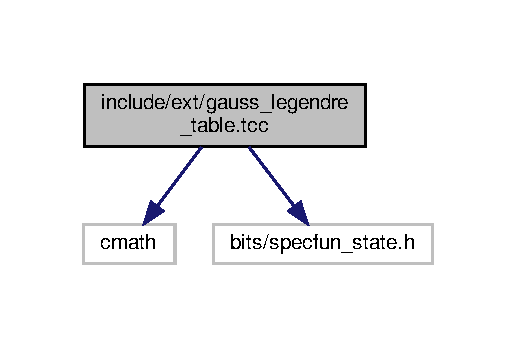
\includegraphics[width=248pt]{gauss__legendre__table_8tcc__incl}
\end{center}
\end{figure}
This graph shows which files directly or indirectly include this file\+:
\nopagebreak
\begin{figure}[H]
\begin{center}
\leavevmode
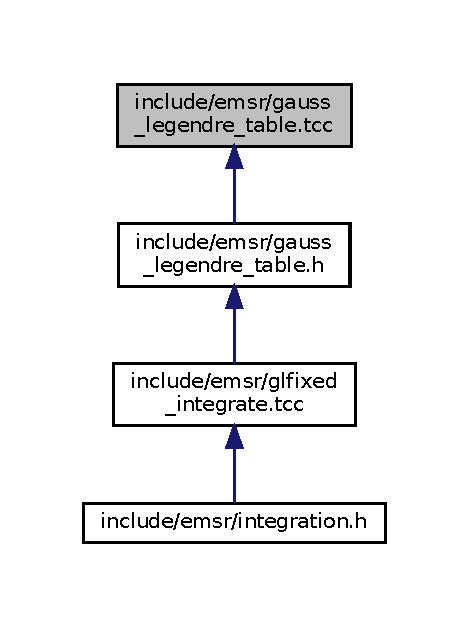
\includegraphics[width=215pt]{gauss__legendre__table_8tcc__dep__incl}
\end{center}
\end{figure}
\subsection*{Namespaces}
\begin{DoxyCompactItemize}
\item 
 \hyperlink{namespace____gnu__cxx}{\+\_\+\+\_\+gnu\+\_\+cxx}
\end{DoxyCompactItemize}
\subsection*{Macros}
\begin{DoxyCompactItemize}
\item 
\#define \hyperlink{gauss__legendre__table_8tcc_ac44e5cd6caf00a0fdea6bfe181c66868}{G\+A\+U\+S\+S\+\_\+\+L\+E\+G\+E\+N\+D\+R\+E\+\_\+\+T\+A\+B\+L\+E\+\_\+\+T\+CC}~1
\end{DoxyCompactItemize}


\subsection{Macro Definition Documentation}
\mbox{\Hypertarget{gauss__legendre__table_8tcc_ac44e5cd6caf00a0fdea6bfe181c66868}\label{gauss__legendre__table_8tcc_ac44e5cd6caf00a0fdea6bfe181c66868}} 
\index{gauss\+\_\+legendre\+\_\+table.\+tcc@{gauss\+\_\+legendre\+\_\+table.\+tcc}!G\+A\+U\+S\+S\+\_\+\+L\+E\+G\+E\+N\+D\+R\+E\+\_\+\+T\+A\+B\+L\+E\+\_\+\+T\+CC@{G\+A\+U\+S\+S\+\_\+\+L\+E\+G\+E\+N\+D\+R\+E\+\_\+\+T\+A\+B\+L\+E\+\_\+\+T\+CC}}
\index{G\+A\+U\+S\+S\+\_\+\+L\+E\+G\+E\+N\+D\+R\+E\+\_\+\+T\+A\+B\+L\+E\+\_\+\+T\+CC@{G\+A\+U\+S\+S\+\_\+\+L\+E\+G\+E\+N\+D\+R\+E\+\_\+\+T\+A\+B\+L\+E\+\_\+\+T\+CC}!gauss\+\_\+legendre\+\_\+table.\+tcc@{gauss\+\_\+legendre\+\_\+table.\+tcc}}
\subsubsection{\texorpdfstring{G\+A\+U\+S\+S\+\_\+\+L\+E\+G\+E\+N\+D\+R\+E\+\_\+\+T\+A\+B\+L\+E\+\_\+\+T\+CC}{GAUSS\_LEGENDRE\_TABLE\_TCC}}
{\footnotesize\ttfamily \#define G\+A\+U\+S\+S\+\_\+\+L\+E\+G\+E\+N\+D\+R\+E\+\_\+\+T\+A\+B\+L\+E\+\_\+\+T\+CC~1}



Definition at line 28 of file gauss\+\_\+legendre\+\_\+table.\+tcc.


\hypertarget{gauss__quadrature_8h}{}\doxysection{include/emsr/gauss\+\_\+quadrature.h File Reference}
\label{gauss__quadrature_8h}\index{include/emsr/gauss\_quadrature.h@{include/emsr/gauss\_quadrature.h}}
{\ttfamily \#include $<$type\+\_\+traits$>$}\newline
{\ttfamily \#include $<$vector$>$}\newline
Include dependency graph for gauss\+\_\+quadrature.\+h\+:
\nopagebreak
\begin{figure}[H]
\begin{center}
\leavevmode
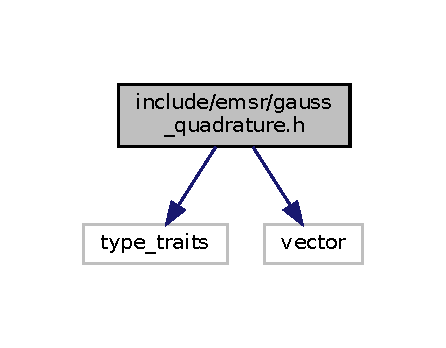
\includegraphics[width=214pt]{gauss__quadrature_8h__incl}
\end{center}
\end{figure}
This graph shows which files directly or indirectly include this file\+:
\nopagebreak
\begin{figure}[H]
\begin{center}
\leavevmode
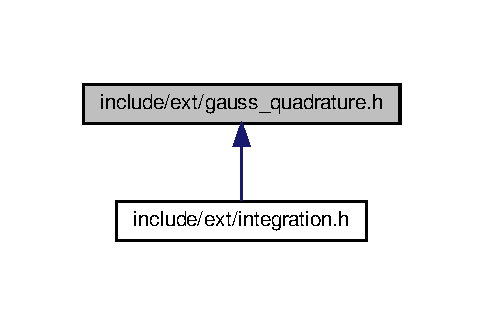
\includegraphics[width=225pt]{gauss__quadrature_8h__dep__incl}
\end{center}
\end{figure}
\doxysubsection*{Classes}
\begin{DoxyCompactItemize}
\item 
struct \mbox{\hyperlink{structemsr_1_1fixed__gauss__chebyshev__t__integral}{emsr\+::fixed\+\_\+gauss\+\_\+chebyshev\+\_\+t\+\_\+integral$<$ Tp $>$}}
\item 
struct \mbox{\hyperlink{structemsr_1_1fixed__gauss__chebyshev__u__integral}{emsr\+::fixed\+\_\+gauss\+\_\+chebyshev\+\_\+u\+\_\+integral$<$ Tp $>$}}
\item 
struct \mbox{\hyperlink{structemsr_1_1fixed__gauss__chebyshev__v__integral}{emsr\+::fixed\+\_\+gauss\+\_\+chebyshev\+\_\+v\+\_\+integral$<$ Tp $>$}}
\item 
struct \mbox{\hyperlink{structemsr_1_1fixed__gauss__chebyshev__w__integral}{emsr\+::fixed\+\_\+gauss\+\_\+chebyshev\+\_\+w\+\_\+integral$<$ Tp $>$}}
\item 
struct \mbox{\hyperlink{structemsr_1_1fixed__gauss__exponential__integral}{emsr\+::fixed\+\_\+gauss\+\_\+exponential\+\_\+integral$<$ Tp $>$}}
\item 
struct \mbox{\hyperlink{structemsr_1_1fixed__gauss__gegenbauer__integral}{emsr\+::fixed\+\_\+gauss\+\_\+gegenbauer\+\_\+integral$<$ Tp $>$}}
\item 
struct \mbox{\hyperlink{structemsr_1_1fixed__gauss__hermite__integral}{emsr\+::fixed\+\_\+gauss\+\_\+hermite\+\_\+integral$<$ Tp $>$}}
\item 
struct \mbox{\hyperlink{structemsr_1_1fixed__gauss__jacobi__integral}{emsr\+::fixed\+\_\+gauss\+\_\+jacobi\+\_\+integral$<$ Tp $>$}}
\item 
struct \mbox{\hyperlink{structemsr_1_1fixed__gauss__laguerre__integral}{emsr\+::fixed\+\_\+gauss\+\_\+laguerre\+\_\+integral$<$ Tp $>$}}
\item 
struct \mbox{\hyperlink{structemsr_1_1fixed__gauss__legendre__integral}{emsr\+::fixed\+\_\+gauss\+\_\+legendre\+\_\+integral$<$ Tp $>$}}
\item 
struct \mbox{\hyperlink{structemsr_1_1fixed__gauss__rational__integral}{emsr\+::fixed\+\_\+gauss\+\_\+rational\+\_\+integral$<$ Tp $>$}}
\end{DoxyCompactItemize}
\doxysubsection*{Namespaces}
\begin{DoxyCompactItemize}
\item 
 \mbox{\hyperlink{namespaceemsr}{emsr}}
\end{DoxyCompactItemize}
\doxysubsection*{Functions}
\begin{DoxyCompactItemize}
\item 
{\footnotesize template$<$typename Tp , typename Func\+Tp $>$ }\\fixed\+\_\+integral\+\_\+t$<$ \mbox{\hyperlink{test__integral_8tcc_a82f489a4943d33943d0b0f781a801283}{Tp}}, std\+::invoke\+\_\+result\+\_\+t$<$ Func\+Tp, \mbox{\hyperlink{test__integral_8tcc_a82f489a4943d33943d0b0f781a801283}{Tp}} $>$ $>$ \mbox{\hyperlink{namespaceemsr_a0978b98459c510ae37addb62d88dc0f7}{emsr\+::integrate\+\_\+fixed\+\_\+gauss\+\_\+chebyshev\+\_\+t}} (int n, Func\+Tp func, \mbox{\hyperlink{test__integral_8tcc_a82f489a4943d33943d0b0f781a801283}{Tp}} lower, \mbox{\hyperlink{test__integral_8tcc_a82f489a4943d33943d0b0f781a801283}{Tp}} upper)
\item 
{\footnotesize template$<$typename Tp , typename Func\+Tp $>$ }\\fixed\+\_\+integral\+\_\+t$<$ \mbox{\hyperlink{test__integral_8tcc_a82f489a4943d33943d0b0f781a801283}{Tp}}, std\+::invoke\+\_\+result\+\_\+t$<$ Func\+Tp, \mbox{\hyperlink{test__integral_8tcc_a82f489a4943d33943d0b0f781a801283}{Tp}} $>$ $>$ \mbox{\hyperlink{namespaceemsr_a04eaad6590c96dbae3f5216853fe21d2}{emsr\+::integrate\+\_\+fixed\+\_\+gauss\+\_\+chebyshev\+\_\+u}} (int n, Func\+Tp func, \mbox{\hyperlink{test__integral_8tcc_a82f489a4943d33943d0b0f781a801283}{Tp}} lower, \mbox{\hyperlink{test__integral_8tcc_a82f489a4943d33943d0b0f781a801283}{Tp}} upper)
\item 
{\footnotesize template$<$typename Tp , typename Func\+Tp $>$ }\\fixed\+\_\+integral\+\_\+t$<$ \mbox{\hyperlink{test__integral_8tcc_a82f489a4943d33943d0b0f781a801283}{Tp}}, std\+::invoke\+\_\+result\+\_\+t$<$ Func\+Tp, \mbox{\hyperlink{test__integral_8tcc_a82f489a4943d33943d0b0f781a801283}{Tp}} $>$ $>$ \mbox{\hyperlink{namespaceemsr_a4970fcee45fe48617ea6601dbca76fdf}{emsr\+::integrate\+\_\+fixed\+\_\+gauss\+\_\+chebyshev\+\_\+v}} (int n, Func\+Tp func, \mbox{\hyperlink{test__integral_8tcc_a82f489a4943d33943d0b0f781a801283}{Tp}} lower, \mbox{\hyperlink{test__integral_8tcc_a82f489a4943d33943d0b0f781a801283}{Tp}} upper)
\item 
{\footnotesize template$<$typename Tp , typename Func\+Tp $>$ }\\fixed\+\_\+integral\+\_\+t$<$ \mbox{\hyperlink{test__integral_8tcc_a82f489a4943d33943d0b0f781a801283}{Tp}}, std\+::invoke\+\_\+result\+\_\+t$<$ Func\+Tp, \mbox{\hyperlink{test__integral_8tcc_a82f489a4943d33943d0b0f781a801283}{Tp}} $>$ $>$ \mbox{\hyperlink{namespaceemsr_a594466ba613e946727ffa0fe9b6581cb}{emsr\+::integrate\+\_\+fixed\+\_\+gauss\+\_\+chebyshev\+\_\+w}} (int n, Func\+Tp func, \mbox{\hyperlink{test__integral_8tcc_a82f489a4943d33943d0b0f781a801283}{Tp}} lower, \mbox{\hyperlink{test__integral_8tcc_a82f489a4943d33943d0b0f781a801283}{Tp}} upper)
\item 
{\footnotesize template$<$typename Tp , typename Func\+Tp $>$ }\\fixed\+\_\+integral\+\_\+t$<$ \mbox{\hyperlink{test__integral_8tcc_a82f489a4943d33943d0b0f781a801283}{Tp}}, std\+::invoke\+\_\+result\+\_\+t$<$ Func\+Tp, \mbox{\hyperlink{test__integral_8tcc_a82f489a4943d33943d0b0f781a801283}{Tp}} $>$ $>$ \mbox{\hyperlink{namespaceemsr_aec0a1347fb6b1ab3d26bf180322b82c8}{emsr\+::integrate\+\_\+fixed\+\_\+gauss\+\_\+exponential}} (int n, \mbox{\hyperlink{test__integral_8tcc_a82f489a4943d33943d0b0f781a801283}{Tp}} alf, Func\+Tp func, \mbox{\hyperlink{test__integral_8tcc_a82f489a4943d33943d0b0f781a801283}{Tp}} lower, \mbox{\hyperlink{test__integral_8tcc_a82f489a4943d33943d0b0f781a801283}{Tp}} upper)
\item 
{\footnotesize template$<$typename Tp , typename Func\+Tp $>$ }\\fixed\+\_\+integral\+\_\+t$<$ \mbox{\hyperlink{test__integral_8tcc_a82f489a4943d33943d0b0f781a801283}{Tp}}, std\+::invoke\+\_\+result\+\_\+t$<$ Func\+Tp, \mbox{\hyperlink{test__integral_8tcc_a82f489a4943d33943d0b0f781a801283}{Tp}} $>$ $>$ \mbox{\hyperlink{namespaceemsr_a768bb88ef10cc3f8c244ebe866f9acc4}{emsr\+::integrate\+\_\+fixed\+\_\+gauss\+\_\+gegenbauer}} (int n, \mbox{\hyperlink{test__integral_8tcc_a82f489a4943d33943d0b0f781a801283}{Tp}} lambda, Func\+Tp func, \mbox{\hyperlink{test__integral_8tcc_a82f489a4943d33943d0b0f781a801283}{Tp}} lower, \mbox{\hyperlink{test__integral_8tcc_a82f489a4943d33943d0b0f781a801283}{Tp}} upper)
\item 
{\footnotesize template$<$typename Tp , typename Func\+Tp $>$ }\\fixed\+\_\+integral\+\_\+t$<$ \mbox{\hyperlink{test__integral_8tcc_a82f489a4943d33943d0b0f781a801283}{Tp}}, std\+::invoke\+\_\+result\+\_\+t$<$ Func\+Tp, \mbox{\hyperlink{test__integral_8tcc_a82f489a4943d33943d0b0f781a801283}{Tp}} $>$ $>$ \mbox{\hyperlink{namespaceemsr_a7ea1e8349f04f299b1f30a7f17a925ba}{emsr\+::integrate\+\_\+fixed\+\_\+gauss\+\_\+hermite}} (int n, \mbox{\hyperlink{test__integral_8tcc_a82f489a4943d33943d0b0f781a801283}{Tp}} alf, Func\+Tp func, \mbox{\hyperlink{test__integral_8tcc_a82f489a4943d33943d0b0f781a801283}{Tp}} lower, \mbox{\hyperlink{test__integral_8tcc_a82f489a4943d33943d0b0f781a801283}{Tp}} upper)
\item 
{\footnotesize template$<$typename Tp , typename Func\+Tp $>$ }\\fixed\+\_\+integral\+\_\+t$<$ \mbox{\hyperlink{test__integral_8tcc_a82f489a4943d33943d0b0f781a801283}{Tp}}, std\+::invoke\+\_\+result\+\_\+t$<$ Func\+Tp, \mbox{\hyperlink{test__integral_8tcc_a82f489a4943d33943d0b0f781a801283}{Tp}} $>$ $>$ \mbox{\hyperlink{namespaceemsr_a3a6069ca8ceb0f74bd43801b92dbe78e}{emsr\+::integrate\+\_\+fixed\+\_\+gauss\+\_\+jacobi}} (int n, \mbox{\hyperlink{test__integral_8tcc_a82f489a4943d33943d0b0f781a801283}{Tp}} alf, \mbox{\hyperlink{test__integral_8tcc_a82f489a4943d33943d0b0f781a801283}{Tp}} bet, Func\+Tp func, \mbox{\hyperlink{test__integral_8tcc_a82f489a4943d33943d0b0f781a801283}{Tp}} lower, \mbox{\hyperlink{test__integral_8tcc_a82f489a4943d33943d0b0f781a801283}{Tp}} upper)
\item 
{\footnotesize template$<$typename Tp , typename Func\+Tp $>$ }\\fixed\+\_\+integral\+\_\+t$<$ \mbox{\hyperlink{test__integral_8tcc_a82f489a4943d33943d0b0f781a801283}{Tp}}, std\+::invoke\+\_\+result\+\_\+t$<$ Func\+Tp, \mbox{\hyperlink{test__integral_8tcc_a82f489a4943d33943d0b0f781a801283}{Tp}} $>$ $>$ \mbox{\hyperlink{namespaceemsr_a8fab35bf5229c05b1028feb97ea648d0}{emsr\+::integrate\+\_\+fixed\+\_\+gauss\+\_\+laguerre}} (int n, \mbox{\hyperlink{test__integral_8tcc_a82f489a4943d33943d0b0f781a801283}{Tp}} alf, Func\+Tp func, \mbox{\hyperlink{test__integral_8tcc_a82f489a4943d33943d0b0f781a801283}{Tp}} lower, \mbox{\hyperlink{test__integral_8tcc_a82f489a4943d33943d0b0f781a801283}{Tp}} upper)
\item 
{\footnotesize template$<$typename Tp , typename Func\+Tp $>$ }\\fixed\+\_\+integral\+\_\+t$<$ \mbox{\hyperlink{test__integral_8tcc_a82f489a4943d33943d0b0f781a801283}{Tp}}, std\+::invoke\+\_\+result\+\_\+t$<$ Func\+Tp, \mbox{\hyperlink{test__integral_8tcc_a82f489a4943d33943d0b0f781a801283}{Tp}} $>$ $>$ \mbox{\hyperlink{namespaceemsr_a40bbd15e2a1f850380807fdeb5209151}{emsr\+::integrate\+\_\+fixed\+\_\+gauss\+\_\+legendre}} (int n, Func\+Tp func, \mbox{\hyperlink{test__integral_8tcc_a82f489a4943d33943d0b0f781a801283}{Tp}} lower, \mbox{\hyperlink{test__integral_8tcc_a82f489a4943d33943d0b0f781a801283}{Tp}} upper)
\item 
{\footnotesize template$<$typename Tp , typename Func\+Tp $>$ }\\fixed\+\_\+integral\+\_\+t$<$ \mbox{\hyperlink{test__integral_8tcc_a82f489a4943d33943d0b0f781a801283}{Tp}}, std\+::invoke\+\_\+result\+\_\+t$<$ Func\+Tp, \mbox{\hyperlink{test__integral_8tcc_a82f489a4943d33943d0b0f781a801283}{Tp}} $>$ $>$ \mbox{\hyperlink{namespaceemsr_ac3912f6d5c51a7fec97ae5cbe3bcc81d}{emsr\+::integrate\+\_\+fixed\+\_\+gauss\+\_\+rational}} (int n, \mbox{\hyperlink{test__integral_8tcc_a82f489a4943d33943d0b0f781a801283}{Tp}} alf, \mbox{\hyperlink{test__integral_8tcc_a82f489a4943d33943d0b0f781a801283}{Tp}} bet, Func\+Tp func, \mbox{\hyperlink{test__integral_8tcc_a82f489a4943d33943d0b0f781a801283}{Tp}} lower, \mbox{\hyperlink{test__integral_8tcc_a82f489a4943d33943d0b0f781a801283}{Tp}} upper)
\end{DoxyCompactItemize}

\hypertarget{gauss__quadrature_8tcc}{}\section{include/ext/gauss\+\_\+quadrature.tcc File Reference}
\label{gauss__quadrature_8tcc}\index{include/ext/gauss\+\_\+quadrature.\+tcc@{include/ext/gauss\+\_\+quadrature.\+tcc}}
{\ttfamily \#include $<$cmath$>$}\newline
Include dependency graph for gauss\+\_\+quadrature.\+tcc\+:
\nopagebreak
\begin{figure}[H]
\begin{center}
\leavevmode
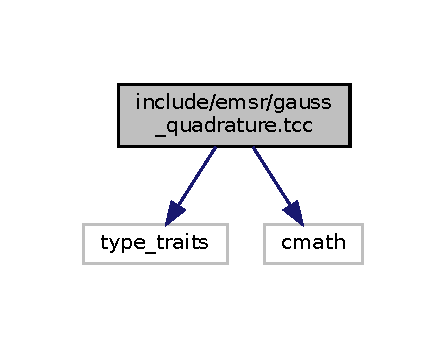
\includegraphics[width=241pt]{gauss__quadrature_8tcc__incl}
\end{center}
\end{figure}
This graph shows which files directly or indirectly include this file\+:
\nopagebreak
\begin{figure}[H]
\begin{center}
\leavevmode
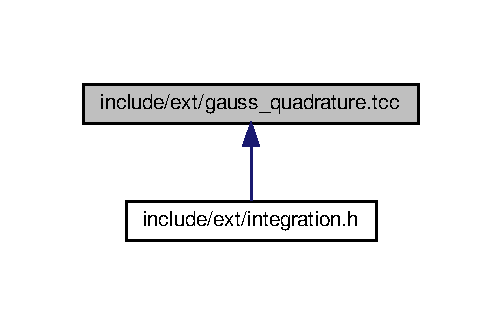
\includegraphics[width=241pt]{gauss__quadrature_8tcc__dep__incl}
\end{center}
\end{figure}
\subsection*{Namespaces}
\begin{DoxyCompactItemize}
\item 
 \hyperlink{namespace____gnu__cxx}{\+\_\+\+\_\+gnu\+\_\+cxx}
\item 
 \hyperlink{namespace____gnu__cxx_1_1____detail}{\+\_\+\+\_\+gnu\+\_\+cxx\+::\+\_\+\+\_\+detail}
\end{DoxyCompactItemize}
\subsection*{Macros}
\begin{DoxyCompactItemize}
\item 
\#define \hyperlink{gauss__quadrature_8tcc_a15767214c365a41207a7325e17fa335b}{G\+A\+U\+S\+S\+\_\+\+Q\+U\+A\+D\+R\+A\+T\+U\+R\+E\+\_\+\+T\+CC}~1
\end{DoxyCompactItemize}
\subsection*{Functions}
\begin{DoxyCompactItemize}
\item 
{\footnotesize template$<$typename \+\_\+\+Tp , typename \+\_\+\+In\+Iter , typename \+\_\+\+Out\+Iter $>$ }\\void \hyperlink{namespace____gnu__cxx_1_1____detail_aa9f299bb7c04606a9a9aab3ab9e4f4c8}{\+\_\+\+\_\+gnu\+\_\+cxx\+::\+\_\+\+\_\+detail\+::\+\_\+\+\_\+golub\+\_\+welsch} (\+\_\+\+Tp \+\_\+\+\_\+moment0, int \+\_\+\+\_\+n, \+\_\+\+In\+Iter \&\+\_\+\+\_\+diag, \+\_\+\+In\+Iter \&\+\_\+\+\_\+subd, \+\_\+\+Out\+Iter \&\+\_\+\+\_\+pt, \+\_\+\+Out\+Iter \&\+\_\+\+\_\+wt)
\end{DoxyCompactItemize}


\subsection{Macro Definition Documentation}
\mbox{\Hypertarget{gauss__quadrature_8tcc_a15767214c365a41207a7325e17fa335b}\label{gauss__quadrature_8tcc_a15767214c365a41207a7325e17fa335b}} 
\index{gauss\+\_\+quadrature.\+tcc@{gauss\+\_\+quadrature.\+tcc}!G\+A\+U\+S\+S\+\_\+\+Q\+U\+A\+D\+R\+A\+T\+U\+R\+E\+\_\+\+T\+CC@{G\+A\+U\+S\+S\+\_\+\+Q\+U\+A\+D\+R\+A\+T\+U\+R\+E\+\_\+\+T\+CC}}
\index{G\+A\+U\+S\+S\+\_\+\+Q\+U\+A\+D\+R\+A\+T\+U\+R\+E\+\_\+\+T\+CC@{G\+A\+U\+S\+S\+\_\+\+Q\+U\+A\+D\+R\+A\+T\+U\+R\+E\+\_\+\+T\+CC}!gauss\+\_\+quadrature.\+tcc@{gauss\+\_\+quadrature.\+tcc}}
\subsubsection{\texorpdfstring{G\+A\+U\+S\+S\+\_\+\+Q\+U\+A\+D\+R\+A\+T\+U\+R\+E\+\_\+\+T\+CC}{GAUSS\_QUADRATURE\_TCC}}
{\footnotesize\ttfamily \#define G\+A\+U\+S\+S\+\_\+\+Q\+U\+A\+D\+R\+A\+T\+U\+R\+E\+\_\+\+T\+CC~1}



Definition at line 22 of file gauss\+\_\+quadrature.\+tcc.


\hypertarget{glfixed__integrate_8tcc}{}\doxysection{include/emsr/glfixed\+\_\+integrate.tcc File Reference}
\label{glfixed__integrate_8tcc}\index{include/emsr/glfixed\_integrate.tcc@{include/emsr/glfixed\_integrate.tcc}}
{\ttfamily \#include $<$type\+\_\+traits$>$}\newline
{\ttfamily \#include $<$emsr/gauss\+\_\+legendre\+\_\+table.\+h$>$}\newline
Include dependency graph for glfixed\+\_\+integrate.\+tcc\+:
\nopagebreak
\begin{figure}[H]
\begin{center}
\leavevmode
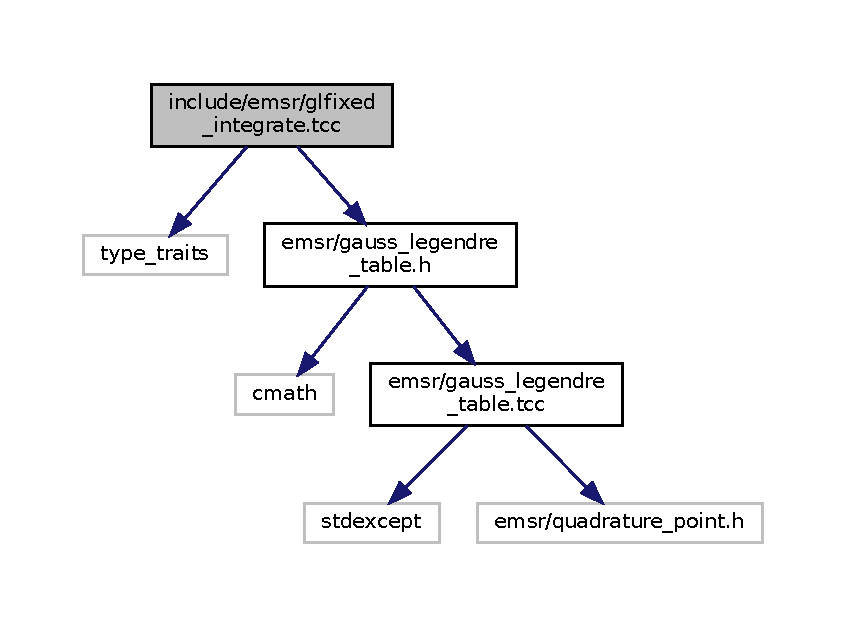
\includegraphics[width=347pt]{glfixed__integrate_8tcc__incl}
\end{center}
\end{figure}
This graph shows which files directly or indirectly include this file\+:
\nopagebreak
\begin{figure}[H]
\begin{center}
\leavevmode
\includegraphics[width=225pt]{glfixed__integrate_8tcc__dep__incl}
\end{center}
\end{figure}
\doxysubsection*{Namespaces}
\begin{DoxyCompactItemize}
\item 
 \mbox{\hyperlink{namespaceemsr}{emsr}}
\end{DoxyCompactItemize}
\doxysubsection*{Macros}
\begin{DoxyCompactItemize}
\item 
\#define \mbox{\hyperlink{glfixed__integrate_8tcc_a59b18c28cc328f58f042a33acd5d46aa}{GLFIXED\+\_\+\+INTEGRATE\+\_\+\+TCC}}~1
\end{DoxyCompactItemize}
\doxysubsection*{Variables}
\begin{DoxyCompactItemize}
\item 
{\footnotesize template$<$typename Tp , typename Func\+Tp $>$ }\\decltype(std\+::invoke\+\_\+result\+\_\+t$<$ Func\+Tp, \mbox{\hyperlink{test__integral_8tcc_a82f489a4943d33943d0b0f781a801283}{Tp}} $>$\{\} $\ast$\mbox{\hyperlink{test__integral_8tcc_a82f489a4943d33943d0b0f781a801283}{Tp}}\{\} \mbox{\hyperlink{namespaceemsr_a7aaa9f8ceaf4c26bb5e38bfce4ef9fe0}{emsr\+::glfixed\+\_\+integrate}} )(const gauss\+\_\+legendre\+\_\+table$<$ \mbox{\hyperlink{test__integral_8tcc_a82f489a4943d33943d0b0f781a801283}{Tp}} $>$ \&t, Func\+Tp func, \mbox{\hyperlink{test__integral_8tcc_a82f489a4943d33943d0b0f781a801283}{Tp}} lower, \mbox{\hyperlink{test__integral_8tcc_a82f489a4943d33943d0b0f781a801283}{Tp}} upper)
\end{DoxyCompactItemize}


\doxysubsection{Macro Definition Documentation}
\mbox{\Hypertarget{glfixed__integrate_8tcc_a59b18c28cc328f58f042a33acd5d46aa}\label{glfixed__integrate_8tcc_a59b18c28cc328f58f042a33acd5d46aa}} 
\index{glfixed\_integrate.tcc@{glfixed\_integrate.tcc}!GLFIXED\_INTEGRATE\_TCC@{GLFIXED\_INTEGRATE\_TCC}}
\index{GLFIXED\_INTEGRATE\_TCC@{GLFIXED\_INTEGRATE\_TCC}!glfixed\_integrate.tcc@{glfixed\_integrate.tcc}}
\doxysubsubsection{\texorpdfstring{GLFIXED\_INTEGRATE\_TCC}{GLFIXED\_INTEGRATE\_TCC}}
{\footnotesize\ttfamily \#define GLFIXED\+\_\+\+INTEGRATE\+\_\+\+TCC~1}



Definition at line 22 of file glfixed\+\_\+integrate.\+tcc.


\hypertarget{integration_8h}{}\section{include/ext/integration.h File Reference}
\label{integration_8h}\index{include/ext/integration.\+h@{include/ext/integration.\+h}}
{\ttfamily \#include $<$limits$>$}\newline
{\ttfamily \#include $<$tuple$>$}\newline
{\ttfamily \#include $<$ext/math\+\_\+constants.\+h$>$}\newline
{\ttfamily \#include $<$ext/quadrature\+\_\+point.\+h$>$}\newline
{\ttfamily \#include $<$ext/gauss\+\_\+kronrod\+\_\+integral.\+h$>$}\newline
{\ttfamily \#include $<$ext/trapezoid\+\_\+integral.\+h$>$}\newline
{\ttfamily \#include $<$ext/midpoint\+\_\+integral.\+h$>$}\newline
{\ttfamily \#include $<$ext/simpson\+\_\+integral.\+h$>$}\newline
{\ttfamily \#include $<$ext/gauss\+\_\+quadrature.\+h$>$}\newline
{\ttfamily \#include $<$ext/trapezoid\+\_\+integral.\+tcc$>$}\newline
{\ttfamily \#include $<$ext/midpoint\+\_\+integral.\+tcc$>$}\newline
{\ttfamily \#include $<$ext/simpson\+\_\+integral.\+tcc$>$}\newline
{\ttfamily \#include $<$ext/gauss\+\_\+kronrod\+\_\+integral.\+tcc$>$}\newline
{\ttfamily \#include $<$ext/qag\+\_\+integrate.\+tcc$>$}\newline
{\ttfamily \#include $<$ext/qags\+\_\+integrate.\+tcc$>$}\newline
{\ttfamily \#include $<$ext/qng\+\_\+integrate.\+tcc$>$}\newline
{\ttfamily \#include $<$ext/qagp\+\_\+integrate.\+tcc$>$}\newline
{\ttfamily \#include $<$ext/qcheb\+\_\+integrate.\+tcc$>$}\newline
{\ttfamily \#include $<$ext/qawc\+\_\+integrate.\+tcc$>$}\newline
{\ttfamily \#include $<$ext/qaws\+\_\+integrate.\+tcc$>$}\newline
{\ttfamily \#include $<$ext/qawo\+\_\+integrate.\+tcc$>$}\newline
{\ttfamily \#include $<$ext/qawf\+\_\+integrate.\+tcc$>$}\newline
{\ttfamily \#include $<$ext/glfixed\+\_\+integrate.\+tcc$>$}\newline
{\ttfamily \#include $<$ext/cquad\+\_\+integrate.\+tcc$>$}\newline
{\ttfamily \#include $<$ext/double\+\_\+exp\+\_\+integrate.\+tcc$>$}\newline
{\ttfamily \#include $<$ext/gauss\+\_\+quadrature.\+tcc$>$}\newline
{\ttfamily \#include $<$ext/integration.\+tcc$>$}\newline
Include dependency graph for integration.\+h\+:
\nopagebreak
\begin{figure}[H]
\begin{center}
\leavevmode
\includegraphics[width=350pt]{integration_8h__incl}
\end{center}
\end{figure}
\subsection*{Classes}
\begin{DoxyCompactItemize}
\item 
struct \hyperlink{struct____gnu__cxx_1_1adaptive__integral__t}{\+\_\+\+\_\+gnu\+\_\+cxx\+::adaptive\+\_\+integral\+\_\+t$<$ \+\_\+\+Tp, \+\_\+\+Ret\+Tp $>$}
\item 
struct \hyperlink{struct____gnu__cxx_1_1error__tolerance__t}{\+\_\+\+\_\+gnu\+\_\+cxx\+::error\+\_\+tolerance\+\_\+t$<$ \+\_\+\+Tp $>$}
\item 
struct \hyperlink{struct____gnu__cxx_1_1fixed__integral__t}{\+\_\+\+\_\+gnu\+\_\+cxx\+::fixed\+\_\+integral\+\_\+t$<$ \+\_\+\+Tp, \+\_\+\+Ret\+Tp $>$}
\end{DoxyCompactItemize}
\subsection*{Namespaces}
\begin{DoxyCompactItemize}
\item 
 \hyperlink{namespace____gnu__cxx}{\+\_\+\+\_\+gnu\+\_\+cxx}
\end{DoxyCompactItemize}
\subsection*{Functions}
\begin{DoxyCompactItemize}
\item 
{\footnotesize template$<$typename \+\_\+\+Tp , typename \+\_\+\+Func\+Tp $>$ }\\auto \hyperlink{namespace____gnu__cxx_aa449f51cfcccb7983ff2703333ffb41e}{\+\_\+\+\_\+gnu\+\_\+cxx\+::integrate} (\+\_\+\+Func\+Tp \+\_\+\+\_\+func, \+\_\+\+Tp \+\_\+\+\_\+lower, \+\_\+\+Tp \+\_\+\+\_\+upper, \+\_\+\+Tp \+\_\+\+\_\+max\+\_\+abs\+\_\+error, \+\_\+\+Tp \+\_\+\+\_\+max\+\_\+rel\+\_\+error, std\+::size\+\_\+t \+\_\+\+\_\+max\+\_\+iter=1024, Kronrod\+\_\+\+Rule \+\_\+\+\_\+qkintrule=Kronrod\+\_\+21) -\/$>$ adaptive\+\_\+integral\+\_\+t$<$ \+\_\+\+Tp, std\+::invoke\+\_\+result\+\_\+t$<$ \+\_\+\+Func\+Tp, \+\_\+\+Tp $>$$>$
\item 
{\footnotesize template$<$typename \+\_\+\+Tp , typename \+\_\+\+Func\+Tp $>$ }\\auto \hyperlink{namespace____gnu__cxx_a609c33bc2044563a11ebb05ddcd7b4bb}{\+\_\+\+\_\+gnu\+\_\+cxx\+::integrate\+\_\+cauchy\+\_\+principal\+\_\+value} (\+\_\+\+Func\+Tp \+\_\+\+\_\+func, \+\_\+\+Tp \+\_\+\+\_\+lower, \+\_\+\+Tp \+\_\+\+\_\+upper, \+\_\+\+Tp \+\_\+\+\_\+center, \+\_\+\+Tp \+\_\+\+\_\+max\+\_\+abs\+\_\+err, \+\_\+\+Tp \+\_\+\+\_\+max\+\_\+rel\+\_\+err, std\+::size\+\_\+t \+\_\+\+\_\+max\+\_\+iter=1024) -\/$>$ adaptive\+\_\+integral\+\_\+t$<$ \+\_\+\+Tp, std\+::invoke\+\_\+result\+\_\+t$<$ \+\_\+\+Func\+Tp, \+\_\+\+Tp $>$$>$
\item 
{\footnotesize template$<$typename \+\_\+\+Tp , typename \+\_\+\+Func\+Tp $>$ }\\auto \hyperlink{namespace____gnu__cxx_ad578040e44241fb45ed76360108667e9}{\+\_\+\+\_\+gnu\+\_\+cxx\+::integrate\+\_\+clenshaw\+\_\+curtis} (\+\_\+\+Func\+Tp \+\_\+\+\_\+func, \+\_\+\+Tp \+\_\+\+\_\+lower, \+\_\+\+Tp \+\_\+\+\_\+upper, \+\_\+\+Tp \+\_\+\+\_\+max\+\_\+abs\+\_\+error, \+\_\+\+Tp \+\_\+\+\_\+max\+\_\+rel\+\_\+error, std\+::size\+\_\+t \+\_\+\+\_\+max\+\_\+iter=1024) -\/$>$ adaptive\+\_\+integral\+\_\+t$<$ \+\_\+\+Tp, std\+::invoke\+\_\+result\+\_\+t$<$ \+\_\+\+Func\+Tp, \+\_\+\+Tp $>$$>$
\item 
{\footnotesize template$<$typename \+\_\+\+Tp , typename \+\_\+\+Func\+Tp $>$ }\\adaptive\+\_\+integral\+\_\+t$<$ \+\_\+\+Tp, std\+::invoke\+\_\+result\+\_\+t$<$ \+\_\+\+Func\+Tp, \+\_\+\+Tp $>$ $>$ \hyperlink{namespace____gnu__cxx_a8d2d406894714b19396add57a77260c4}{\+\_\+\+\_\+gnu\+\_\+cxx\+::integrate\+\_\+exp\+\_\+sinh} (\+\_\+\+Func\+Tp \+\_\+\+\_\+func, \+\_\+\+Tp \+\_\+\+\_\+a, \+\_\+\+Tp \+\_\+\+\_\+max\+\_\+abs\+\_\+err, \+\_\+\+Tp \+\_\+\+\_\+max\+\_\+rel\+\_\+err, int \+\_\+\+\_\+max\+\_\+iter)
\item 
{\footnotesize template$<$typename \+\_\+\+Tp , typename \+\_\+\+Func\+Tp $>$ }\\fixed\+\_\+integral\+\_\+t$<$ \+\_\+\+Tp, std\+::invoke\+\_\+result\+\_\+t$<$ \+\_\+\+Func\+Tp, \+\_\+\+Tp $>$ $>$ \hyperlink{namespace____gnu__cxx_a3ab6a5df23f812f6760750d8fb4b3098}{\+\_\+\+\_\+gnu\+\_\+cxx\+::integrate\+\_\+fixed\+\_\+gauss\+\_\+chebyshev\+\_\+t} (int \+\_\+\+\_\+n, \+\_\+\+Func\+Tp \+\_\+\+\_\+func, \+\_\+\+Tp \+\_\+\+\_\+a, \+\_\+\+Tp \+\_\+\+\_\+b)
\item 
{\footnotesize template$<$typename \+\_\+\+Tp , typename \+\_\+\+Func\+Tp $>$ }\\fixed\+\_\+integral\+\_\+t$<$ \+\_\+\+Tp, std\+::invoke\+\_\+result\+\_\+t$<$ \+\_\+\+Func\+Tp, \+\_\+\+Tp $>$ $>$ \hyperlink{namespace____gnu__cxx_a38001a3f61a4fc4757b038d3db0180ca}{\+\_\+\+\_\+gnu\+\_\+cxx\+::integrate\+\_\+fixed\+\_\+gauss\+\_\+chebyshev\+\_\+u} (int \+\_\+\+\_\+n, \+\_\+\+Func\+Tp \+\_\+\+\_\+func, \+\_\+\+Tp \+\_\+\+\_\+a, \+\_\+\+Tp \+\_\+\+\_\+b)
\item 
{\footnotesize template$<$typename \+\_\+\+Tp , typename \+\_\+\+Func\+Tp $>$ }\\fixed\+\_\+integral\+\_\+t$<$ \+\_\+\+Tp, std\+::invoke\+\_\+result\+\_\+t$<$ \+\_\+\+Func\+Tp, \+\_\+\+Tp $>$ $>$ \hyperlink{namespace____gnu__cxx_a1d79fed8d593be6c4c1f1cc2ecf92785}{\+\_\+\+\_\+gnu\+\_\+cxx\+::integrate\+\_\+fixed\+\_\+gauss\+\_\+chebyshev\+\_\+v} (int \+\_\+\+\_\+n, \+\_\+\+Func\+Tp \+\_\+\+\_\+func, \+\_\+\+Tp \+\_\+\+\_\+a, \+\_\+\+Tp \+\_\+\+\_\+b)
\item 
{\footnotesize template$<$typename \+\_\+\+Tp , typename \+\_\+\+Func\+Tp $>$ }\\fixed\+\_\+integral\+\_\+t$<$ \+\_\+\+Tp, std\+::invoke\+\_\+result\+\_\+t$<$ \+\_\+\+Func\+Tp, \+\_\+\+Tp $>$ $>$ \hyperlink{namespace____gnu__cxx_a45de562834adf3f097e4ad9a3eb75444}{\+\_\+\+\_\+gnu\+\_\+cxx\+::integrate\+\_\+fixed\+\_\+gauss\+\_\+chebyshev\+\_\+w} (int \+\_\+\+\_\+n, \+\_\+\+Func\+Tp \+\_\+\+\_\+func, \+\_\+\+Tp \+\_\+\+\_\+a, \+\_\+\+Tp \+\_\+\+\_\+b)
\item 
{\footnotesize template$<$typename \+\_\+\+Tp , typename \+\_\+\+Func\+Tp $>$ }\\fixed\+\_\+integral\+\_\+t$<$ \+\_\+\+Tp, std\+::invoke\+\_\+result\+\_\+t$<$ \+\_\+\+Func\+Tp, \+\_\+\+Tp $>$ $>$ \hyperlink{namespace____gnu__cxx_ac7e616f825ae281bc831d8743bb7b501}{\+\_\+\+\_\+gnu\+\_\+cxx\+::integrate\+\_\+fixed\+\_\+gauss\+\_\+exponential} (int \+\_\+\+\_\+n, \+\_\+\+Tp \+\_\+\+\_\+alf, \+\_\+\+Func\+Tp \+\_\+\+\_\+func, \+\_\+\+Tp \+\_\+\+\_\+a, \+\_\+\+Tp \+\_\+\+\_\+b)
\item 
{\footnotesize template$<$typename \+\_\+\+Tp , typename \+\_\+\+Func\+Tp $>$ }\\fixed\+\_\+integral\+\_\+t$<$ \+\_\+\+Tp, std\+::invoke\+\_\+result\+\_\+t$<$ \+\_\+\+Func\+Tp, \+\_\+\+Tp $>$ $>$ \hyperlink{namespace____gnu__cxx_aaf74d571f8c3ccc7a6c7f7c64e9edb29}{\+\_\+\+\_\+gnu\+\_\+cxx\+::integrate\+\_\+fixed\+\_\+gauss\+\_\+gegenbauer} (int \+\_\+\+\_\+n, \+\_\+\+Tp \+\_\+\+\_\+lambda, \+\_\+\+Func\+Tp \+\_\+\+\_\+func, \+\_\+\+Tp \+\_\+\+\_\+a, \+\_\+\+Tp \+\_\+\+\_\+b)
\item 
{\footnotesize template$<$typename \+\_\+\+Tp , typename \+\_\+\+Func\+Tp $>$ }\\fixed\+\_\+integral\+\_\+t$<$ \+\_\+\+Tp, std\+::invoke\+\_\+result\+\_\+t$<$ \+\_\+\+Func\+Tp, \+\_\+\+Tp $>$ $>$ \hyperlink{namespace____gnu__cxx_a248024d8be18e0354ce80967dcba919a}{\+\_\+\+\_\+gnu\+\_\+cxx\+::integrate\+\_\+fixed\+\_\+gauss\+\_\+hermite} (int \+\_\+\+\_\+n, \+\_\+\+Tp \+\_\+\+\_\+alf, \+\_\+\+Func\+Tp \+\_\+\+\_\+func, \+\_\+\+Tp \+\_\+\+\_\+a, \+\_\+\+Tp \+\_\+\+\_\+b)
\item 
{\footnotesize template$<$typename \+\_\+\+Tp , typename \+\_\+\+Func\+Tp $>$ }\\fixed\+\_\+integral\+\_\+t$<$ \+\_\+\+Tp, std\+::invoke\+\_\+result\+\_\+t$<$ \+\_\+\+Func\+Tp, \+\_\+\+Tp $>$ $>$ \hyperlink{namespace____gnu__cxx_a798b6524ce81200fec2e9e1712fcdd35}{\+\_\+\+\_\+gnu\+\_\+cxx\+::integrate\+\_\+fixed\+\_\+gauss\+\_\+jacobi} (int \+\_\+\+\_\+n, \+\_\+\+Tp \+\_\+\+\_\+alf, \+\_\+\+Tp \+\_\+\+\_\+bet, \+\_\+\+Func\+Tp \+\_\+\+\_\+func, \+\_\+\+Tp \+\_\+\+\_\+a, \+\_\+\+Tp \+\_\+\+\_\+b)
\item 
{\footnotesize template$<$typename \+\_\+\+Tp , typename \+\_\+\+Func\+Tp $>$ }\\fixed\+\_\+integral\+\_\+t$<$ \+\_\+\+Tp, std\+::invoke\+\_\+result\+\_\+t$<$ \+\_\+\+Func\+Tp, \+\_\+\+Tp $>$ $>$ \hyperlink{namespace____gnu__cxx_a9f7832337c163702c3ede5dbceb3c8e0}{\+\_\+\+\_\+gnu\+\_\+cxx\+::integrate\+\_\+fixed\+\_\+gauss\+\_\+laguerre} (int \+\_\+\+\_\+n, \+\_\+\+Tp \+\_\+\+\_\+alf, \+\_\+\+Func\+Tp \+\_\+\+\_\+func, \+\_\+\+Tp \+\_\+\+\_\+a, \+\_\+\+Tp \+\_\+\+\_\+b)
\item 
{\footnotesize template$<$typename \+\_\+\+Tp , typename \+\_\+\+Func\+Tp $>$ }\\fixed\+\_\+integral\+\_\+t$<$ \+\_\+\+Tp, std\+::invoke\+\_\+result\+\_\+t$<$ \+\_\+\+Func\+Tp, \+\_\+\+Tp $>$ $>$ \hyperlink{namespace____gnu__cxx_a9115896dfa9f35b53dbb720347a69a1c}{\+\_\+\+\_\+gnu\+\_\+cxx\+::integrate\+\_\+fixed\+\_\+gauss\+\_\+legendre} (int \+\_\+\+\_\+n, \+\_\+\+Func\+Tp \+\_\+\+\_\+func, \+\_\+\+Tp \+\_\+\+\_\+a, \+\_\+\+Tp \+\_\+\+\_\+b)
\item 
{\footnotesize template$<$typename \+\_\+\+Tp , typename \+\_\+\+Func\+Tp $>$ }\\fixed\+\_\+integral\+\_\+t$<$ \+\_\+\+Tp, std\+::invoke\+\_\+result\+\_\+t$<$ \+\_\+\+Func\+Tp, \+\_\+\+Tp $>$ $>$ \hyperlink{namespace____gnu__cxx_ae7ec81551d6057e093b7b2991ad6f3fa}{\+\_\+\+\_\+gnu\+\_\+cxx\+::integrate\+\_\+fixed\+\_\+gauss\+\_\+rational} (int \+\_\+\+\_\+n, \+\_\+\+Tp \+\_\+\+\_\+alf, \+\_\+\+Tp \+\_\+\+\_\+bet, \+\_\+\+Func\+Tp \+\_\+\+\_\+func, \+\_\+\+Tp \+\_\+\+\_\+a, \+\_\+\+Tp \+\_\+\+\_\+b)
\item 
{\footnotesize template$<$typename \+\_\+\+Tp , typename \+\_\+\+Func\+Tp $>$ }\\auto \hyperlink{namespace____gnu__cxx_aaf3bee7e1617cc1ef517b155e8b14e87}{\+\_\+\+\_\+gnu\+\_\+cxx\+::integrate\+\_\+kronrod\+\_\+singular} (\+\_\+\+Func\+Tp \+\_\+\+\_\+func, \+\_\+\+Tp \+\_\+\+\_\+lower, \+\_\+\+Tp \+\_\+\+\_\+upper, \+\_\+\+Tp \+\_\+\+\_\+max\+\_\+abs\+\_\+error, \+\_\+\+Tp \+\_\+\+\_\+max\+\_\+rel\+\_\+error, std\+::size\+\_\+t \+\_\+\+\_\+max\+\_\+iter=1024) -\/$>$ adaptive\+\_\+integral\+\_\+t$<$ \+\_\+\+Tp, std\+::invoke\+\_\+result\+\_\+t$<$ \+\_\+\+Func\+Tp, \+\_\+\+Tp $>$$>$
\item 
{\footnotesize template$<$typename \+\_\+\+Tp , typename \+\_\+\+Func\+Tp $>$ }\\auto \hyperlink{namespace____gnu__cxx_a2a1c7fcbb716c0f1f8f93ce3893b564a}{\+\_\+\+\_\+gnu\+\_\+cxx\+::integrate\+\_\+lower\+\_\+minf} (\+\_\+\+Func\+Tp \+\_\+\+\_\+func, \+\_\+\+Tp \+\_\+\+\_\+lower, \+\_\+\+Tp \+\_\+\+\_\+max\+\_\+abs\+\_\+error, \+\_\+\+Tp \+\_\+\+\_\+max\+\_\+rel\+\_\+error, std\+::size\+\_\+t \+\_\+\+\_\+max\+\_\+iter=1024, Kronrod\+\_\+\+Rule \+\_\+\+\_\+qkintrule=Kronrod\+\_\+21) -\/$>$ adaptive\+\_\+integral\+\_\+t$<$ \+\_\+\+Tp, std\+::invoke\+\_\+result\+\_\+t$<$ \+\_\+\+Func\+Tp, \+\_\+\+Tp $>$$>$
\item 
{\footnotesize template$<$typename \+\_\+\+Tp , typename \+\_\+\+Func\+Tp $>$ }\\auto \hyperlink{namespace____gnu__cxx_ad1f0fd43b7a498328749e924085b4fc1}{\+\_\+\+\_\+gnu\+\_\+cxx\+::integrate\+\_\+lower\+\_\+pinf} (\+\_\+\+Func\+Tp \+\_\+\+\_\+func, \+\_\+\+Tp \+\_\+\+\_\+lower, \+\_\+\+Tp \+\_\+\+\_\+max\+\_\+abs\+\_\+error, \+\_\+\+Tp \+\_\+\+\_\+max\+\_\+rel\+\_\+error, std\+::size\+\_\+t \+\_\+\+\_\+max\+\_\+iter=1024, Kronrod\+\_\+\+Rule \+\_\+\+\_\+qkintrule=Kronrod\+\_\+21) -\/$>$ adaptive\+\_\+integral\+\_\+t$<$ \+\_\+\+Tp, std\+::invoke\+\_\+result\+\_\+t$<$ \+\_\+\+Func\+Tp, \+\_\+\+Tp $>$$>$
\item 
{\footnotesize template$<$typename \+\_\+\+Tp , typename \+\_\+\+Func\+Tp $>$ }\\adaptive\+\_\+integral\+\_\+t$<$ \+\_\+\+Tp, std\+::invoke\+\_\+result\+\_\+t$<$ \+\_\+\+Func\+Tp, \+\_\+\+Tp $>$ $>$ \hyperlink{namespace____gnu__cxx_af2f2b282767e1e4e9529c398dcf092dc}{\+\_\+\+\_\+gnu\+\_\+cxx\+::integrate\+\_\+midpoint} (\+\_\+\+Func\+Tp \+\_\+\+\_\+func, \+\_\+\+Tp \+\_\+\+\_\+a, \+\_\+\+Tp \+\_\+\+\_\+b, \+\_\+\+Tp \+\_\+\+\_\+max\+\_\+abs\+\_\+err, \+\_\+\+Tp \+\_\+\+\_\+max\+\_\+rel\+\_\+err, int \+\_\+\+\_\+max\+\_\+iter)
\item 
{\footnotesize template$<$typename \+\_\+\+Tp , typename \+\_\+\+Func\+Tp $>$ }\\auto \hyperlink{namespace____gnu__cxx_a4c63281e592f7319501e228c7f2e6eca}{\+\_\+\+\_\+gnu\+\_\+cxx\+::integrate\+\_\+minf\+\_\+pinf} (\+\_\+\+Func\+Tp \+\_\+\+\_\+func, \+\_\+\+Tp \+\_\+\+\_\+max\+\_\+abs\+\_\+error, \+\_\+\+Tp \+\_\+\+\_\+max\+\_\+rel\+\_\+error, std\+::size\+\_\+t \+\_\+\+\_\+max\+\_\+iter=1024, Kronrod\+\_\+\+Rule \+\_\+\+\_\+qkintrule=Kronrod\+\_\+21) -\/$>$ adaptive\+\_\+integral\+\_\+t$<$ \+\_\+\+Tp, std\+::invoke\+\_\+result\+\_\+t$<$ \+\_\+\+Func\+Tp, \+\_\+\+Tp $>$$>$
\item 
{\footnotesize template$<$typename \+\_\+\+Tp , typename \+\_\+\+Func\+Tp $>$ }\\auto \hyperlink{namespace____gnu__cxx_ac452c1c660d47daf605eda7b395ba497}{\+\_\+\+\_\+gnu\+\_\+cxx\+::integrate\+\_\+minf\+\_\+upper} (\+\_\+\+Func\+Tp \+\_\+\+\_\+func, \+\_\+\+Tp \+\_\+\+\_\+upper, \+\_\+\+Tp \+\_\+\+\_\+max\+\_\+abs\+\_\+error, \+\_\+\+Tp \+\_\+\+\_\+max\+\_\+rel\+\_\+error, std\+::size\+\_\+t \+\_\+\+\_\+max\+\_\+iter=1024, Kronrod\+\_\+\+Rule \+\_\+\+\_\+qkintrule=Kronrod\+\_\+21) -\/$>$ adaptive\+\_\+integral\+\_\+t$<$ \+\_\+\+Tp, std\+::invoke\+\_\+result\+\_\+t$<$ \+\_\+\+Func\+Tp, \+\_\+\+Tp $>$$>$
\item 
{\footnotesize template$<$typename \+\_\+\+Func\+Tp , typename \+\_\+\+Fwd\+Iter , typename \+\_\+\+Tp $>$ }\\auto \hyperlink{namespace____gnu__cxx_ae77d3835b02400d9fb8f00c6db994cc5}{\+\_\+\+\_\+gnu\+\_\+cxx\+::integrate\+\_\+multisingular} (\+\_\+\+Func\+Tp \+\_\+\+\_\+func, \+\_\+\+Fwd\+Iter \+\_\+\+\_\+ptbeg, \+\_\+\+Fwd\+Iter \+\_\+\+\_\+ptend, \+\_\+\+Tp \+\_\+\+\_\+max\+\_\+abs\+\_\+error, \+\_\+\+Tp \+\_\+\+\_\+max\+\_\+rel\+\_\+error, std\+::size\+\_\+t \+\_\+\+\_\+max\+\_\+iter=1024) -\/$>$ adaptive\+\_\+integral\+\_\+t$<$ \+\_\+\+Tp, std\+::invoke\+\_\+result\+\_\+t$<$ \+\_\+\+Func\+Tp, \+\_\+\+Tp $>$$>$
\item 
{\footnotesize template$<$typename \+\_\+\+Tp , typename \+\_\+\+Func\+Tp $>$ }\\auto \hyperlink{namespace____gnu__cxx_aa3b36aa34ddfb56a7c5b50438ca812c1}{\+\_\+\+\_\+gnu\+\_\+cxx\+::integrate\+\_\+oscillatory} (\+\_\+\+Func\+Tp \+\_\+\+\_\+func, \+\_\+\+Tp \+\_\+\+\_\+lower, \+\_\+\+Tp \+\_\+\+\_\+upper, \+\_\+\+Tp \+\_\+\+\_\+max\+\_\+abs\+\_\+error, \+\_\+\+Tp \+\_\+\+\_\+max\+\_\+rel\+\_\+error, std\+::size\+\_\+t \+\_\+\+\_\+max\+\_\+iter=1024) -\/$>$ adaptive\+\_\+integral\+\_\+t$<$ \+\_\+\+Tp, std\+::invoke\+\_\+result\+\_\+t$<$ \+\_\+\+Func\+Tp, \+\_\+\+Tp $>$$>$
\item 
{\footnotesize template$<$typename \+\_\+\+Tp , typename \+\_\+\+Func\+Tp $>$ }\\auto \hyperlink{namespace____gnu__cxx_ae3b63cd8d35caff65b0dda0194373b85}{\+\_\+\+\_\+gnu\+\_\+cxx\+::integrate\+\_\+patterson} (\+\_\+\+Func\+Tp \+\_\+\+\_\+func, \+\_\+\+Tp \+\_\+\+\_\+lower, \+\_\+\+Tp \+\_\+\+\_\+upper, \+\_\+\+Tp \+\_\+\+\_\+max\+\_\+abs\+\_\+error, \+\_\+\+Tp \+\_\+\+\_\+max\+\_\+rel\+\_\+error) -\/$>$ adaptive\+\_\+integral\+\_\+t$<$ \+\_\+\+Tp, std\+::invoke\+\_\+result\+\_\+t$<$ \+\_\+\+Func\+Tp, \+\_\+\+Tp $>$$>$
\item 
{\footnotesize template$<$typename \+\_\+\+Tp , typename \+\_\+\+Func\+Tp $>$ }\\auto \hyperlink{namespace____gnu__cxx_a091752f3c6d7a289ec0e0228385468c5}{\+\_\+\+\_\+gnu\+\_\+cxx\+::integrate\+\_\+pinf\+\_\+upper} (\+\_\+\+Func\+Tp \+\_\+\+\_\+func, \+\_\+\+Tp \+\_\+\+\_\+upper, \+\_\+\+Tp \+\_\+\+\_\+max\+\_\+abs\+\_\+error, \+\_\+\+Tp \+\_\+\+\_\+max\+\_\+rel\+\_\+error, std\+::size\+\_\+t \+\_\+\+\_\+max\+\_\+iter=1024, Kronrod\+\_\+\+Rule \+\_\+\+\_\+qkintrule=Kronrod\+\_\+21) -\/$>$ adaptive\+\_\+integral\+\_\+t$<$ \+\_\+\+Tp, std\+::invoke\+\_\+result\+\_\+t$<$ \+\_\+\+Func\+Tp, \+\_\+\+Tp $>$$>$
\item 
{\footnotesize template$<$typename \+\_\+\+Tp , typename \+\_\+\+Func\+Tp $>$ }\\auto \hyperlink{namespace____gnu__cxx_ab7b0961f8fb1553f8a70902b110a22ef}{\+\_\+\+\_\+gnu\+\_\+cxx\+::integrate\+\_\+singular} (\+\_\+\+Func\+Tp \+\_\+\+\_\+func, \+\_\+\+Tp \+\_\+\+\_\+lower, \+\_\+\+Tp \+\_\+\+\_\+upper, \+\_\+\+Tp \+\_\+\+\_\+max\+\_\+abs\+\_\+error, \+\_\+\+Tp \+\_\+\+\_\+max\+\_\+rel\+\_\+error, std\+::size\+\_\+t \+\_\+\+\_\+max\+\_\+iter=1024) -\/$>$ adaptive\+\_\+integral\+\_\+t$<$ \+\_\+\+Tp, std\+::invoke\+\_\+result\+\_\+t$<$ \+\_\+\+Func\+Tp, \+\_\+\+Tp $>$$>$
\item 
{\footnotesize template$<$typename \+\_\+\+Tp , typename \+\_\+\+Func\+Tp $>$ }\\auto \hyperlink{namespace____gnu__cxx_acac4890eaca9950b39a06e980f846868}{\+\_\+\+\_\+gnu\+\_\+cxx\+::integrate\+\_\+singular\+\_\+endpoints} (\+\_\+\+Func\+Tp \+\_\+\+\_\+func, \+\_\+\+Tp \+\_\+\+\_\+lower, \+\_\+\+Tp \+\_\+\+\_\+upper, \+\_\+\+Tp \+\_\+\+\_\+alpha, \+\_\+\+Tp \+\_\+\+\_\+beta, int \+\_\+\+\_\+mu, int \+\_\+\+\_\+nu, \+\_\+\+Tp \+\_\+\+\_\+max\+\_\+abs\+\_\+error, \+\_\+\+Tp \+\_\+\+\_\+max\+\_\+rel\+\_\+error, std\+::size\+\_\+t \+\_\+\+\_\+max\+\_\+iter=1024) -\/$>$ adaptive\+\_\+integral\+\_\+t$<$ \+\_\+\+Tp, std\+::invoke\+\_\+result\+\_\+t$<$ \+\_\+\+Func\+Tp, \+\_\+\+Tp $>$$>$
\item 
{\footnotesize template$<$typename \+\_\+\+Tp , typename \+\_\+\+Func\+Tp $>$ }\\auto \hyperlink{namespace____gnu__cxx_a31bafd8ae702762989558b29593ffe6c}{\+\_\+\+\_\+gnu\+\_\+cxx\+::integrate\+\_\+singular\+\_\+lower\+\_\+minf} (\+\_\+\+Func\+Tp \+\_\+\+\_\+func, \+\_\+\+Tp \+\_\+\+\_\+lower, \+\_\+\+Tp \+\_\+\+\_\+max\+\_\+abs\+\_\+error, \+\_\+\+Tp \+\_\+\+\_\+max\+\_\+rel\+\_\+error, std\+::size\+\_\+t \+\_\+\+\_\+max\+\_\+iter=1024) -\/$>$ adaptive\+\_\+integral\+\_\+t$<$ \+\_\+\+Tp, std\+::invoke\+\_\+result\+\_\+t$<$ \+\_\+\+Func\+Tp, \+\_\+\+Tp $>$$>$
\item 
{\footnotesize template$<$typename \+\_\+\+Tp , typename \+\_\+\+Func\+Tp $>$ }\\auto \hyperlink{namespace____gnu__cxx_aead3b14ccced37c14f64ecd358a2b0c8}{\+\_\+\+\_\+gnu\+\_\+cxx\+::integrate\+\_\+singular\+\_\+lower\+\_\+pinf} (\+\_\+\+Func\+Tp \+\_\+\+\_\+func, \+\_\+\+Tp \+\_\+\+\_\+lower, \+\_\+\+Tp \+\_\+\+\_\+max\+\_\+abs\+\_\+error, \+\_\+\+Tp \+\_\+\+\_\+max\+\_\+rel\+\_\+error, std\+::size\+\_\+t \+\_\+\+\_\+max\+\_\+iter=1024) -\/$>$ adaptive\+\_\+integral\+\_\+t$<$ \+\_\+\+Tp, std\+::invoke\+\_\+result\+\_\+t$<$ \+\_\+\+Func\+Tp, \+\_\+\+Tp $>$$>$
\item 
{\footnotesize template$<$typename \+\_\+\+Tp , typename \+\_\+\+Func\+Tp $>$ }\\auto \hyperlink{namespace____gnu__cxx_a10e839f46ed2fda3a57ed7710a51cfbc}{\+\_\+\+\_\+gnu\+\_\+cxx\+::integrate\+\_\+singular\+\_\+minf\+\_\+pinf} (\+\_\+\+Func\+Tp \+\_\+\+\_\+func, \+\_\+\+Tp \+\_\+\+\_\+max\+\_\+abs\+\_\+error, \+\_\+\+Tp \+\_\+\+\_\+max\+\_\+rel\+\_\+error, std\+::size\+\_\+t \+\_\+\+\_\+max\+\_\+iter=1024) -\/$>$ adaptive\+\_\+integral\+\_\+t$<$ \+\_\+\+Tp, std\+::invoke\+\_\+result\+\_\+t$<$ \+\_\+\+Func\+Tp, \+\_\+\+Tp $>$$>$
\item 
{\footnotesize template$<$typename \+\_\+\+Tp , typename \+\_\+\+Func\+Tp $>$ }\\auto \hyperlink{namespace____gnu__cxx_add15531ace95d18f7fe52a63dd8a7113}{\+\_\+\+\_\+gnu\+\_\+cxx\+::integrate\+\_\+singular\+\_\+minf\+\_\+upper} (\+\_\+\+Func\+Tp \+\_\+\+\_\+func, \+\_\+\+Tp \+\_\+\+\_\+upper, \+\_\+\+Tp \+\_\+\+\_\+max\+\_\+abs\+\_\+error, \+\_\+\+Tp \+\_\+\+\_\+max\+\_\+rel\+\_\+error, std\+::size\+\_\+t \+\_\+\+\_\+max\+\_\+iter=1024) -\/$>$ adaptive\+\_\+integral\+\_\+t$<$ \+\_\+\+Tp, std\+::invoke\+\_\+result\+\_\+t$<$ \+\_\+\+Func\+Tp, \+\_\+\+Tp $>$$>$
\item 
{\footnotesize template$<$typename \+\_\+\+Tp , typename \+\_\+\+Func\+Tp $>$ }\\auto \hyperlink{namespace____gnu__cxx_aa9f2cb4d805bca6241e46ab08437c25d}{\+\_\+\+\_\+gnu\+\_\+cxx\+::integrate\+\_\+singular\+\_\+pinf\+\_\+upper} (\+\_\+\+Func\+Tp \+\_\+\+\_\+func, \+\_\+\+Tp \+\_\+\+\_\+upper, \+\_\+\+Tp \+\_\+\+\_\+max\+\_\+abs\+\_\+error, \+\_\+\+Tp \+\_\+\+\_\+max\+\_\+rel\+\_\+error, std\+::size\+\_\+t \+\_\+\+\_\+max\+\_\+iter=1024) -\/$>$ adaptive\+\_\+integral\+\_\+t$<$ \+\_\+\+Tp, std\+::invoke\+\_\+result\+\_\+t$<$ \+\_\+\+Func\+Tp, \+\_\+\+Tp $>$$>$
\item 
{\footnotesize template$<$typename \+\_\+\+Tp , typename \+\_\+\+Func\+Tp $>$ }\\adaptive\+\_\+integral\+\_\+t$<$ \+\_\+\+Tp, std\+::invoke\+\_\+result\+\_\+t$<$ \+\_\+\+Func\+Tp, \+\_\+\+Tp $>$ $>$ \hyperlink{namespace____gnu__cxx_ab28f15831507df5ef94f271648fb2263}{\+\_\+\+\_\+gnu\+\_\+cxx\+::integrate\+\_\+sinh\+\_\+sinh} (\+\_\+\+Func\+Tp \+\_\+\+\_\+func, \+\_\+\+Tp \+\_\+\+\_\+max\+\_\+abs\+\_\+err, \+\_\+\+Tp \+\_\+\+\_\+max\+\_\+rel\+\_\+err, int \+\_\+\+\_\+max\+\_\+iter)
\item 
{\footnotesize template$<$typename \+\_\+\+Tp , typename \+\_\+\+Func\+Tp $>$ }\\adaptive\+\_\+integral\+\_\+t$<$ \+\_\+\+Tp, std\+::invoke\+\_\+result\+\_\+t$<$ \+\_\+\+Func\+Tp, \+\_\+\+Tp $>$ $>$ \hyperlink{namespace____gnu__cxx_a814fe9e5540142d7cfd6513247b73ab5}{\+\_\+\+\_\+gnu\+\_\+cxx\+::integrate\+\_\+tanh\+\_\+sinh} (\+\_\+\+Func\+Tp \+\_\+\+\_\+func, \+\_\+\+Tp \+\_\+\+\_\+a, \+\_\+\+Tp \+\_\+\+\_\+b, \+\_\+\+Tp \+\_\+\+\_\+max\+\_\+abs\+\_\+err, \+\_\+\+Tp \+\_\+\+\_\+max\+\_\+rel\+\_\+err, int \+\_\+\+\_\+max\+\_\+iter)
\item 
{\footnotesize template$<$typename \+\_\+\+Tp , typename \+\_\+\+Func\+Tp $>$ }\\adaptive\+\_\+integral\+\_\+t$<$ \+\_\+\+Tp, std\+::invoke\+\_\+result\+\_\+t$<$ \+\_\+\+Func\+Tp, \+\_\+\+Tp $>$ $>$ \hyperlink{namespace____gnu__cxx_adf9d0d087d69a8a279053edd15487d71}{\+\_\+\+\_\+gnu\+\_\+cxx\+::integrate\+\_\+trapezoid} (\+\_\+\+Func\+Tp \+\_\+\+\_\+func, \+\_\+\+Tp \+\_\+\+\_\+a, \+\_\+\+Tp \+\_\+\+\_\+b, \+\_\+\+Tp \+\_\+\+\_\+max\+\_\+abs\+\_\+err, \+\_\+\+Tp \+\_\+\+\_\+max\+\_\+rel\+\_\+err, int \+\_\+\+\_\+max\+\_\+iter)
\item 
{\footnotesize template$<$typename \+\_\+\+Tp $>$ }\\bool \hyperlink{namespace____gnu__cxx_a86b1d89b2e2cb97614fdf3425d3dccd5}{\+\_\+\+\_\+gnu\+\_\+cxx\+::valid\+\_\+tolerances} (\+\_\+\+Tp \+\_\+\+\_\+max\+\_\+abs\+\_\+err, \+\_\+\+Tp \+\_\+\+\_\+max\+\_\+rel\+\_\+err)
\end{DoxyCompactItemize}

\hypertarget{integration__error_8h}{}\section{include/ext/integration\+\_\+error.h File Reference}
\label{integration__error_8h}\index{include/ext/integration\+\_\+error.\+h@{include/ext/integration\+\_\+error.\+h}}
{\ttfamily \#include $<$cmath$>$}\newline
{\ttfamily \#include $<$limits$>$}\newline
{\ttfamily \#include $<$sstream$>$}\newline
{\ttfamily \#include $<$string\+\_\+view$>$}\newline
Include dependency graph for integration\+\_\+error.\+h\+:
\nopagebreak
\begin{figure}[H]
\begin{center}
\leavevmode
\includegraphics[width=336pt]{integration__error_8h__incl}
\end{center}
\end{figure}
This graph shows which files directly or indirectly include this file\+:
\nopagebreak
\begin{figure}[H]
\begin{center}
\leavevmode
\includegraphics[width=350pt]{integration__error_8h__dep__incl}
\end{center}
\end{figure}
\subsection*{Classes}
\begin{DoxyCompactItemize}
\item 
class \hyperlink{class____gnu__cxx_1_1____integration__error}{\+\_\+\+\_\+gnu\+\_\+cxx\+::\+\_\+\+\_\+integration\+\_\+error$<$ \+\_\+\+Tp $>$}
\end{DoxyCompactItemize}
\subsection*{Namespaces}
\begin{DoxyCompactItemize}
\item 
 \hyperlink{namespace____gnu__cxx}{\+\_\+\+\_\+gnu\+\_\+cxx}
\end{DoxyCompactItemize}
\subsection*{Enumerations}
\begin{DoxyCompactItemize}
\item 
enum \{ \newline
\hyperlink{namespace____gnu__cxx_ad6c62dd86a596716cece6ac2d4cfd4b3ac31eecc280b10dec2efb4a2216ccc2e0}{\+\_\+\+\_\+gnu\+\_\+cxx\+::\+N\+O\+\_\+\+E\+R\+R\+OR}, 
\hyperlink{namespace____gnu__cxx_ad6c62dd86a596716cece6ac2d4cfd4b3a420d46d10205dd953d0ccce5323afc4c}{\+\_\+\+\_\+gnu\+\_\+cxx\+::\+M\+A\+X\+\_\+\+I\+T\+E\+R\+\_\+\+E\+R\+R\+OR}, 
\hyperlink{namespace____gnu__cxx_ad6c62dd86a596716cece6ac2d4cfd4b3a29574de87143c7715e9a138d7340e8ae}{\+\_\+\+\_\+gnu\+\_\+cxx\+::\+R\+O\+U\+N\+D\+O\+F\+F\+\_\+\+E\+R\+R\+OR}, 
\hyperlink{namespace____gnu__cxx_ad6c62dd86a596716cece6ac2d4cfd4b3a8e955ea89d59c116d92f16f345620d04}{\+\_\+\+\_\+gnu\+\_\+cxx\+::\+S\+I\+N\+G\+U\+L\+A\+R\+\_\+\+E\+R\+R\+OR}, 
\newline
\hyperlink{namespace____gnu__cxx_ad6c62dd86a596716cece6ac2d4cfd4b3ac3b74f0b40291f29a3cb3a188412308b}{\+\_\+\+\_\+gnu\+\_\+cxx\+::\+E\+X\+T\+R\+A\+P\+\_\+\+R\+O\+U\+N\+D\+O\+F\+F\+\_\+\+E\+R\+R\+OR}, 
\hyperlink{namespace____gnu__cxx_ad6c62dd86a596716cece6ac2d4cfd4b3a5a36b63b8fa7c921d9332c69416c2686}{\+\_\+\+\_\+gnu\+\_\+cxx\+::\+D\+I\+V\+E\+R\+G\+E\+N\+C\+E\+\_\+\+E\+R\+R\+OR}, 
\hyperlink{namespace____gnu__cxx_ad6c62dd86a596716cece6ac2d4cfd4b3a4c1e6a4f8a49af2eae50e4bf6f93e016}{\+\_\+\+\_\+gnu\+\_\+cxx\+::\+M\+A\+X\+\_\+\+S\+U\+B\+D\+I\+V\+\_\+\+E\+R\+R\+OR}, 
\hyperlink{namespace____gnu__cxx_ad6c62dd86a596716cece6ac2d4cfd4b3ab7427fd44a0ed217814ca07b9b5aba07}{\+\_\+\+\_\+gnu\+\_\+cxx\+::\+T\+O\+L\+E\+R\+A\+N\+C\+E\+\_\+\+E\+R\+R\+OR}, 
\newline
\hyperlink{namespace____gnu__cxx_ad6c62dd86a596716cece6ac2d4cfd4b3a7c57c614db2692fad0a19cb2ded33ed3}{\+\_\+\+\_\+gnu\+\_\+cxx\+::\+U\+N\+K\+N\+O\+W\+N\+\_\+\+E\+R\+R\+OR}
 \}
\end{DoxyCompactItemize}
\subsection*{Functions}
\begin{DoxyCompactItemize}
\item 
{\footnotesize template$<$typename \+\_\+\+Tp $>$ }\\void \hyperlink{namespace____gnu__cxx_a370fd142548c2e9e39e69282b4603317}{\+\_\+\+\_\+gnu\+\_\+cxx\+::\+\_\+\+\_\+check\+\_\+error} (std\+::string\+\_\+view \+\_\+\+\_\+func, int \+\_\+\+\_\+errcode, \+\_\+\+Tp \+\_\+\+\_\+result=std\+::numeric\+\_\+limits$<$ \+\_\+\+Tp $>$\+::quiet\+\_\+\+NaN(), \+\_\+\+Tp \+\_\+\+\_\+abserr=std\+::numeric\+\_\+limits$<$ \+\_\+\+Tp $>$\+::quiet\+\_\+\+NaN())
\item 
{\footnotesize template$<$typename \+\_\+\+Tp $>$ }\\\+\_\+\+Tp \hyperlink{namespace____gnu__cxx_aeff8a54364ae3976f593b8699626a897}{\+\_\+\+\_\+gnu\+\_\+cxx\+::\+\_\+\+\_\+rescale\+\_\+error} (\+\_\+\+Tp \+\_\+\+\_\+err, const \+\_\+\+Tp \+\_\+\+\_\+result\+\_\+abs, const \+\_\+\+Tp \+\_\+\+\_\+result\+\_\+asc)
\item 
{\footnotesize template$<$typename \+\_\+\+Tp $>$ }\\void \hyperlink{namespace____gnu__cxx_a2ae22137ca092b8ae10f4d42b4e32cfb}{\+\_\+\+\_\+gnu\+\_\+cxx\+::\+\_\+\+\_\+throw\+\_\+integration\+\_\+error} (const char $\ast$\+\_\+\+\_\+what, int \+\_\+\+\_\+errcode, \+\_\+\+Tp \+\_\+\+\_\+result=std\+::numeric\+\_\+limits$<$ \+\_\+\+Tp $>$\+::quiet\+\_\+\+NaN(), \+\_\+\+Tp \+\_\+\+\_\+abserr=std\+::numeric\+\_\+limits$<$ \+\_\+\+Tp $>$\+::quiet\+\_\+\+NaN()) \+\_\+\+\_\+attribute\+\_\+\+\_\+((\+\_\+\+\_\+noreturn\+\_\+\+\_\+))
\end{DoxyCompactItemize}

\hypertarget{integration__transform_8h}{}\section{include/ext/integration\+\_\+transform.h File Reference}
\label{integration__transform_8h}\index{include/ext/integration\+\_\+transform.\+h@{include/ext/integration\+\_\+transform.\+h}}
This graph shows which files directly or indirectly include this file\+:
\nopagebreak
\begin{figure}[H]
\begin{center}
\leavevmode
\includegraphics[width=227pt]{integration__transform_8h__dep__incl}
\end{center}
\end{figure}
\subsection*{Classes}
\begin{DoxyCompactItemize}
\item 
struct \hyperlink{struct____gnu__cxx_1_1map__a__pinf}{\+\_\+\+\_\+gnu\+\_\+cxx\+::map\+\_\+a\+\_\+pinf$<$ \+\_\+\+Tp, \+\_\+\+Func\+Tp $>$}
\item 
struct \hyperlink{struct____gnu__cxx_1_1map__minf__b}{\+\_\+\+\_\+gnu\+\_\+cxx\+::map\+\_\+minf\+\_\+b$<$ \+\_\+\+Tp, \+\_\+\+Func\+Tp $>$}
\item 
struct \hyperlink{struct____gnu__cxx_1_1map__minf__pinf}{\+\_\+\+\_\+gnu\+\_\+cxx\+::map\+\_\+minf\+\_\+pinf$<$ \+\_\+\+Tp, \+\_\+\+Func\+Tp $>$}
\item 
struct \hyperlink{struct____gnu__cxx_1_1map__minf__pinf__symm}{\+\_\+\+\_\+gnu\+\_\+cxx\+::map\+\_\+minf\+\_\+pinf\+\_\+symm$<$ \+\_\+\+Tp, \+\_\+\+Func\+Tp $>$}
\item 
struct \hyperlink{struct____gnu__cxx_1_1mapper}{\+\_\+\+\_\+gnu\+\_\+cxx\+::mapper$<$ \+\_\+\+Tp, \+\_\+\+Func\+Tp $>$}
\end{DoxyCompactItemize}
\subsection*{Namespaces}
\begin{DoxyCompactItemize}
\item 
 \hyperlink{namespace____gnu__cxx}{\+\_\+\+\_\+gnu\+\_\+cxx}
\end{DoxyCompactItemize}

\hypertarget{integration__workspace_8h}{}\section{include/ext/integration\+\_\+workspace.h File Reference}
\label{integration__workspace_8h}\index{include/ext/integration\+\_\+workspace.\+h@{include/ext/integration\+\_\+workspace.\+h}}
{\ttfamily \#include $<$algorithm$>$}\newline
{\ttfamily \#include $<$vector$>$}\newline
{\ttfamily \#include $<$limits$>$}\newline
{\ttfamily \#include $<$cmath$>$}\newline
{\ttfamily \#include $<$iosfwd$>$}\newline
{\ttfamily \#include $<$ext/integration\+\_\+workspace.\+tcc$>$}\newline
Include dependency graph for integration\+\_\+workspace.\+h\+:
\nopagebreak
\begin{figure}[H]
\begin{center}
\leavevmode
\includegraphics[width=350pt]{integration__workspace_8h__incl}
\end{center}
\end{figure}
This graph shows which files directly or indirectly include this file\+:
\nopagebreak
\begin{figure}[H]
\begin{center}
\leavevmode
\includegraphics[width=350pt]{integration__workspace_8h__dep__incl}
\end{center}
\end{figure}
\subsection*{Classes}
\begin{DoxyCompactItemize}
\item 
class \hyperlink{class____gnu__cxx_1_1integration__workspace}{\+\_\+\+\_\+gnu\+\_\+cxx\+::integration\+\_\+workspace$<$ \+\_\+\+Tp, \+\_\+\+Ret\+Tp $>$}
\end{DoxyCompactItemize}
\subsection*{Namespaces}
\begin{DoxyCompactItemize}
\item 
 \hyperlink{namespace____gnu__cxx}{\+\_\+\+\_\+gnu\+\_\+cxx}
\end{DoxyCompactItemize}
\subsection*{Functions}
\begin{DoxyCompactItemize}
\item 
{\footnotesize template$<$typename \+\_\+\+Tp , typename \+\_\+\+Ret\+Tp $>$ }\\std\+::ostream \& \hyperlink{namespace____gnu__cxx_a2f2af1d76b024a139e350aa0f81ac272}{\+\_\+\+\_\+gnu\+\_\+cxx\+::operator$<$$<$} (std\+::ostream \&\+\_\+\+\_\+out, const integration\+\_\+workspace$<$ \+\_\+\+Tp, \+\_\+\+Ret\+Tp $>$ \&\+\_\+\+\_\+ws)
\end{DoxyCompactItemize}

\hypertarget{integration__workspace_8tcc}{}\doxysection{include/emsr/integration\+\_\+workspace.tcc File Reference}
\label{integration__workspace_8tcc}\index{include/emsr/integration\_workspace.tcc@{include/emsr/integration\_workspace.tcc}}
{\ttfamily \#include $<$iostream$>$}\newline
{\ttfamily \#include $<$iomanip$>$}\newline
{\ttfamily \#include $<$emsr/integration\+\_\+error.\+h$>$}\newline
Include dependency graph for integration\+\_\+workspace.\+tcc\+:
\nopagebreak
\begin{figure}[H]
\begin{center}
\leavevmode
\includegraphics[width=350pt]{integration__workspace_8tcc__incl}
\end{center}
\end{figure}
This graph shows which files directly or indirectly include this file\+:
\nopagebreak
\begin{figure}[H]
\begin{center}
\leavevmode
\includegraphics[width=350pt]{integration__workspace_8tcc__dep__incl}
\end{center}
\end{figure}
\doxysubsection*{Namespaces}
\begin{DoxyCompactItemize}
\item 
 \mbox{\hyperlink{namespaceemsr}{emsr}}
\end{DoxyCompactItemize}
\doxysubsection*{Macros}
\begin{DoxyCompactItemize}
\item 
\#define \mbox{\hyperlink{integration__workspace_8tcc_a97fff0b995378b137cf1e5424fb2fa95}{INTEGRATION\+\_\+\+WORKSPACE\+\_\+\+TCC}}~1
\end{DoxyCompactItemize}
\doxysubsection*{Functions}
\begin{DoxyCompactItemize}
\item 
{\footnotesize template$<$typename Tp , typename Ret\+Tp $>$ }\\std\+::ostream \& \mbox{\hyperlink{namespaceemsr_af383285041b523a8299e355669f31444}{emsr\+::operator$<$$<$}} (std\+::ostream \&out, const integration\+\_\+workspace$<$ \mbox{\hyperlink{test__integral_8tcc_a82f489a4943d33943d0b0f781a801283}{Tp}}, Ret\+Tp $>$ \&ws)
\end{DoxyCompactItemize}


\doxysubsection{Macro Definition Documentation}
\mbox{\Hypertarget{integration__workspace_8tcc_a97fff0b995378b137cf1e5424fb2fa95}\label{integration__workspace_8tcc_a97fff0b995378b137cf1e5424fb2fa95}} 
\index{integration\_workspace.tcc@{integration\_workspace.tcc}!INTEGRATION\_WORKSPACE\_TCC@{INTEGRATION\_WORKSPACE\_TCC}}
\index{INTEGRATION\_WORKSPACE\_TCC@{INTEGRATION\_WORKSPACE\_TCC}!integration\_workspace.tcc@{integration\_workspace.tcc}}
\doxysubsubsection{\texorpdfstring{INTEGRATION\_WORKSPACE\_TCC}{INTEGRATION\_WORKSPACE\_TCC}}
{\footnotesize\ttfamily \#define INTEGRATION\+\_\+\+WORKSPACE\+\_\+\+TCC~1}



Definition at line 24 of file integration\+\_\+workspace.\+tcc.


\hypertarget{jacobi_8h}{}\section{include/ext/jacobi.h File Reference}
\label{jacobi_8h}\index{include/ext/jacobi.\+h@{include/ext/jacobi.\+h}}


Header file for jacobi library.  


{\ttfamily \#include $<$ext/gauss\+\_\+jacobi\+\_\+interface.\+tcc$>$}\newline
{\ttfamily \#include $<$ext/gauss\+\_\+jacobi\+\_\+integrate.\+tcc$>$}\newline
Include dependency graph for jacobi.\+h\+:
\nopagebreak
\begin{figure}[H]
\begin{center}
\leavevmode
\includegraphics[width=350pt]{jacobi_8h__incl}
\end{center}
\end{figure}
This graph shows which files directly or indirectly include this file\+:
\nopagebreak
\begin{figure}[H]
\begin{center}
\leavevmode
\includegraphics[width=346pt]{jacobi_8h__dep__incl}
\end{center}
\end{figure}
\subsection*{Classes}
\begin{DoxyCompactItemize}
\item 
struct \hyperlink{structjac__quadrature}{jac\+\_\+quadrature$<$ \+\_\+\+Tp $>$}
\begin{DoxyCompactList}\small\item\em Struct used to store information and memory on the quadrature. \end{DoxyCompactList}\end{DoxyCompactItemize}
\subsection*{Enumerations}
\begin{DoxyCompactItemize}
\item 
enum \hyperlink{jacobi_8h_a58cc26f41a96f9220797038d2d3b4c8a}{gauss\+\_\+quad\+\_\+type} \{ \hyperlink{jacobi_8h_a58cc26f41a96f9220797038d2d3b4c8aab15a7891aa5223439e4692a1048cb220}{Gauss}, 
\hyperlink{jacobi_8h_a58cc26f41a96f9220797038d2d3b4c8aadd3020585839e72f9b36b53076db8583}{Gauss\+\_\+\+Lobatto}, 
\hyperlink{jacobi_8h_a58cc26f41a96f9220797038d2d3b4c8aa4c779fa441010c7fbe90c4f40129b584}{Gauss\+\_\+\+Radau\+\_\+lower}, 
\hyperlink{jacobi_8h_a58cc26f41a96f9220797038d2d3b4c8aaabd8ea80c614be833d14da250a270973}{Gauss\+\_\+\+Radau\+\_\+upper}
 \}\begin{DoxyCompactList}\small\item\em Enumeration gor differing types of Gauss quadrature. The gauss\+\_\+quad\+\_\+type is used to determine the boundary condition modifications applied to orthogonal polynomials for quadrature rules. \end{DoxyCompactList}
\end{DoxyCompactItemize}


\subsection{Detailed Description}
Header file for jacobi library. 

The jacobi library implements Jacobi polynomials and Gauss-\/\+Jacobi quadrature related functions. This library was developed to be used in high order finite element methods (Spectral Element/hp methods. The interfaces were inspired by the software Polylib (\href{http://www.nektar.info}{\tt http\+://www.\+nektar.\+info}).

The main sources used to develop this library where\+:

(1) Abramowitz, Milton and Stegun, Irene (editors); \char`\"{}\+Handbook of Mathematical functions\char`\"{}, Dover Publications 1965.

(2) Karniadakis, George Em and Sherwin, Spencer; \char`\"{}\+Spectral/hp Element Methods for Computational
    Fluid Dynamics\char`\"{}, Oxford Science Publications, 2nd edition, 2005.

This software is supposed to be an add-\/on module for the G\+NU Scientific Library 

\subsection{Enumeration Type Documentation}
\mbox{\Hypertarget{jacobi_8h_a58cc26f41a96f9220797038d2d3b4c8a}\label{jacobi_8h_a58cc26f41a96f9220797038d2d3b4c8a}} 
\index{jacobi.\+h@{jacobi.\+h}!gauss\+\_\+quad\+\_\+type@{gauss\+\_\+quad\+\_\+type}}
\index{gauss\+\_\+quad\+\_\+type@{gauss\+\_\+quad\+\_\+type}!jacobi.\+h@{jacobi.\+h}}
\subsubsection{\texorpdfstring{gauss\+\_\+quad\+\_\+type}{gauss\_quad\_type}}
{\footnotesize\ttfamily enum \hyperlink{jacobi_8h_a58cc26f41a96f9220797038d2d3b4c8a}{gauss\+\_\+quad\+\_\+type}}



Enumeration gor differing types of Gauss quadrature. The gauss\+\_\+quad\+\_\+type is used to determine the boundary condition modifications applied to orthogonal polynomials for quadrature rules. 

\begin{DoxyEnumFields}{Enumerator}
\raisebox{\heightof{T}}[0pt][0pt]{\index{Gauss@{Gauss}!jacobi.\+h@{jacobi.\+h}}\index{jacobi.\+h@{jacobi.\+h}!Gauss@{Gauss}}}\mbox{\Hypertarget{jacobi_8h_a58cc26f41a96f9220797038d2d3b4c8aab15a7891aa5223439e4692a1048cb220}\label{jacobi_8h_a58cc26f41a96f9220797038d2d3b4c8aab15a7891aa5223439e4692a1048cb220}} 
Gauss&Gauss quadrature. \\
\hline

\raisebox{\heightof{T}}[0pt][0pt]{\index{Gauss\+\_\+\+Lobatto@{Gauss\+\_\+\+Lobatto}!jacobi.\+h@{jacobi.\+h}}\index{jacobi.\+h@{jacobi.\+h}!Gauss\+\_\+\+Lobatto@{Gauss\+\_\+\+Lobatto}}}\mbox{\Hypertarget{jacobi_8h_a58cc26f41a96f9220797038d2d3b4c8aadd3020585839e72f9b36b53076db8583}\label{jacobi_8h_a58cc26f41a96f9220797038d2d3b4c8aadd3020585839e72f9b36b53076db8583}} 
Gauss\+\_\+\+Lobatto&Gauss-\/\+Lobatto quadrature. \\
\hline

\raisebox{\heightof{T}}[0pt][0pt]{\index{Gauss\+\_\+\+Radau\+\_\+lower@{Gauss\+\_\+\+Radau\+\_\+lower}!jacobi.\+h@{jacobi.\+h}}\index{jacobi.\+h@{jacobi.\+h}!Gauss\+\_\+\+Radau\+\_\+lower@{Gauss\+\_\+\+Radau\+\_\+lower}}}\mbox{\Hypertarget{jacobi_8h_a58cc26f41a96f9220797038d2d3b4c8aa4c779fa441010c7fbe90c4f40129b584}\label{jacobi_8h_a58cc26f41a96f9220797038d2d3b4c8aa4c779fa441010c7fbe90c4f40129b584}} 
Gauss\+\_\+\+Radau\+\_\+lower&Gauss-\/\+Radau quadrature including the node -\/1. \\
\hline

\raisebox{\heightof{T}}[0pt][0pt]{\index{Gauss\+\_\+\+Radau\+\_\+upper@{Gauss\+\_\+\+Radau\+\_\+upper}!jacobi.\+h@{jacobi.\+h}}\index{jacobi.\+h@{jacobi.\+h}!Gauss\+\_\+\+Radau\+\_\+upper@{Gauss\+\_\+\+Radau\+\_\+upper}}}\mbox{\Hypertarget{jacobi_8h_a58cc26f41a96f9220797038d2d3b4c8aaabd8ea80c614be833d14da250a270973}\label{jacobi_8h_a58cc26f41a96f9220797038d2d3b4c8aaabd8ea80c614be833d14da250a270973}} 
Gauss\+\_\+\+Radau\+\_\+upper&Gauss-\/\+Radau quadrature including the node +1. \\
\hline

\end{DoxyEnumFields}


Definition at line 48 of file jacobi.\+h.


\begin{DoxyCode}
49   \{
50     \hyperlink{jacobi_8h_a58cc26f41a96f9220797038d2d3b4c8aab15a7891aa5223439e4692a1048cb220}{Gauss},             \textcolor{comment}{///< Gauss quadrature}
51 \textcolor{comment}{}    \hyperlink{jacobi_8h_a58cc26f41a96f9220797038d2d3b4c8aadd3020585839e72f9b36b53076db8583}{Gauss\_Lobatto},     \textcolor{comment}{///< Gauss-Lobatto quadrature}
52 \textcolor{comment}{}    \hyperlink{jacobi_8h_a58cc26f41a96f9220797038d2d3b4c8aa4c779fa441010c7fbe90c4f40129b584}{Gauss\_Radau\_lower}, \textcolor{comment}{///< Gauss-Radau quadrature including the node -1}
53 \textcolor{comment}{}    \hyperlink{jacobi_8h_a58cc26f41a96f9220797038d2d3b4c8aaabd8ea80c614be833d14da250a270973}{Gauss\_Radau\_upper}  \textcolor{comment}{///< Gauss-Radau quadrature including the node +1}
54 \textcolor{comment}{}  \};
\end{DoxyCode}

\hypertarget{matrix_8h}{}\section{include/ext/matrix.h File Reference}
\label{matrix_8h}\index{include/ext/matrix.\+h@{include/ext/matrix.\+h}}
{\ttfamily \#include $<$ext/matrix.\+tcc$>$}\newline
Include dependency graph for matrix.\+h\+:
\nopagebreak
\begin{figure}[H]
\begin{center}
\leavevmode
\includegraphics[width=182pt]{matrix_8h__incl}
\end{center}
\end{figure}
This graph shows which files directly or indirectly include this file\+:
\nopagebreak
\begin{figure}[H]
\begin{center}
\leavevmode
\includegraphics[width=350pt]{matrix_8h__dep__incl}
\end{center}
\end{figure}
\subsection*{Namespaces}
\begin{DoxyCompactItemize}
\item 
 \hyperlink{namespace____gnu__cxx}{\+\_\+\+\_\+gnu\+\_\+cxx}
\end{DoxyCompactItemize}
\subsection*{Functions}
\begin{DoxyCompactItemize}
\item 
{\footnotesize template$<$typename \+\_\+\+Rand\+Acc\+Iter , typename \+\_\+\+Rand\+Acc\+Iter\+R\+HS $>$ }\\int \hyperlink{namespace____gnu__cxx_a949fff28dbde67178a926d5d11114ebd}{\+\_\+\+\_\+gnu\+\_\+cxx\+::\+\_\+\+S\+\_\+tridiag} (std\+::size\+\_\+t \+\_\+\+\_\+n, \+\_\+\+Rand\+Acc\+Iter \+\_\+\+\_\+supd, \+\_\+\+Rand\+Acc\+Iter \+\_\+\+\_\+diag, \+\_\+\+Rand\+Acc\+Iter \+\_\+\+\_\+subd, \+\_\+\+Rand\+Acc\+Iter\+R\+HS \+\_\+\+\_\+rhs)
\item 
{\footnotesize template$<$typename \+\_\+\+Rand\+Acc\+Iter , typename \+\_\+\+Rand\+Acc\+Iter\+R\+HS $>$ }\\int \hyperlink{namespace____gnu__cxx_a4b9501d94b3eebf5f1ffe990b81cae93}{\+\_\+\+\_\+gnu\+\_\+cxx\+::\+\_\+\+S\+\_\+tridiag\+\_\+symm} (std\+::size\+\_\+t \+\_\+\+\_\+n, \+\_\+\+Rand\+Acc\+Iter \&\+\_\+\+\_\+diag, \+\_\+\+Rand\+Acc\+Iter \&\+\_\+\+\_\+subd, \+\_\+\+Rand\+Acc\+Iter\+R\+HS \&\+\_\+\+\_\+rhs)
\begin{DoxyCompactList}\small\item\em Diagonalize a symmetric tridiagonal matrix. \end{DoxyCompactList}\end{DoxyCompactItemize}

\hypertarget{matrix_8tcc}{}\doxysection{include/emsr/matrix.tcc File Reference}
\label{matrix_8tcc}\index{include/emsr/matrix.tcc@{include/emsr/matrix.tcc}}
{\ttfamily \#include $<$stdexcept$>$}\newline
{\ttfamily \#include $<$type\+\_\+traits$>$}\newline
Include dependency graph for matrix.\+tcc\+:
\nopagebreak
\begin{figure}[H]
\begin{center}
\leavevmode
\includegraphics[width=232pt]{matrix_8tcc__incl}
\end{center}
\end{figure}
This graph shows which files directly or indirectly include this file\+:
\nopagebreak
\begin{figure}[H]
\begin{center}
\leavevmode
\includegraphics[width=350pt]{matrix_8tcc__dep__incl}
\end{center}
\end{figure}
\doxysubsection*{Namespaces}
\begin{DoxyCompactItemize}
\item 
 \mbox{\hyperlink{namespaceemsr}{emsr}}
\end{DoxyCompactItemize}
\doxysubsection*{Macros}
\begin{DoxyCompactItemize}
\item 
\#define \mbox{\hyperlink{matrix_8tcc_a970f96e7f8c79cd72af477aa073d7781}{MATRIX\+\_\+\+TCC}}~1
\end{DoxyCompactItemize}
\doxysubsection*{Functions}
\begin{DoxyCompactItemize}
\item 
{\footnotesize template$<$typename Rand\+Acc\+Iter , typename Rand\+Acc\+Iter\+RHS $>$ }\\int \mbox{\hyperlink{namespaceemsr_a375ffc73e85805ac3e591dac6236339c}{emsr\+::s\+\_\+tridiag}} (size\+\_\+t n, Rand\+Acc\+Iter supd, Rand\+Acc\+Iter diag, Rand\+Acc\+Iter subd, Rand\+Acc\+Iter\+RHS rhs)
\item 
{\footnotesize template$<$typename Rand\+Acc\+Iter , typename Rand\+Acc\+Iter\+RHS $>$ }\\int \mbox{\hyperlink{namespaceemsr_a5cb28151a49c36c36b58a1dc7af7654c}{emsr\+::s\+\_\+tridiag\+\_\+symm}} (std\+::size\+\_\+t n, Rand\+Acc\+Iter \&diag, Rand\+Acc\+Iter \&subd, Rand\+Acc\+Iter\+RHS \&rhs)
\begin{DoxyCompactList}\small\item\em Diagonalize a symmetric tridiagonal matrix. \end{DoxyCompactList}\end{DoxyCompactItemize}


\doxysubsection{Macro Definition Documentation}
\mbox{\Hypertarget{matrix_8tcc_a970f96e7f8c79cd72af477aa073d7781}\label{matrix_8tcc_a970f96e7f8c79cd72af477aa073d7781}} 
\index{matrix.tcc@{matrix.tcc}!MATRIX\_TCC@{MATRIX\_TCC}}
\index{MATRIX\_TCC@{MATRIX\_TCC}!matrix.tcc@{matrix.tcc}}
\doxysubsubsection{\texorpdfstring{MATRIX\_TCC}{MATRIX\_TCC}}
{\footnotesize\ttfamily \#define MATRIX\+\_\+\+TCC~1}



Definition at line 20 of file matrix.\+tcc.


\hypertarget{midpoint__integral_8h}{}\doxysection{include/emsr/midpoint\+\_\+integral.h File Reference}
\label{midpoint__integral_8h}\index{include/emsr/midpoint\_integral.h@{include/emsr/midpoint\_integral.h}}
{\ttfamily \#include $<$type\+\_\+traits$>$}\newline
{\ttfamily \#include $<$cstddef$>$}\newline
{\ttfamily \#include $<$limits$>$}\newline
{\ttfamily \#include $<$emsr/midpoint\+\_\+integral.\+tcc$>$}\newline
Include dependency graph for midpoint\+\_\+integral.\+h\+:
\nopagebreak
\begin{figure}[H]
\begin{center}
\leavevmode
\includegraphics[width=350pt]{midpoint__integral_8h__incl}
\end{center}
\end{figure}
This graph shows which files directly or indirectly include this file\+:
\nopagebreak
\begin{figure}[H]
\begin{center}
\leavevmode
\includegraphics[width=225pt]{midpoint__integral_8h__dep__incl}
\end{center}
\end{figure}
\doxysubsection*{Classes}
\begin{DoxyCompactItemize}
\item 
class \mbox{\hyperlink{classemsr_1_1composite__midpoint__integral}{emsr\+::composite\+\_\+midpoint\+\_\+integral$<$ Tp, Func\+Tp $>$}}
\item 
class \mbox{\hyperlink{classemsr_1_1midpoint__integral}{emsr\+::midpoint\+\_\+integral$<$ Tp, Func\+Tp $>$}}
\end{DoxyCompactItemize}
\doxysubsection*{Namespaces}
\begin{DoxyCompactItemize}
\item 
 \mbox{\hyperlink{namespaceemsr}{emsr}}
\end{DoxyCompactItemize}
\doxysubsection*{Functions}
\begin{DoxyCompactItemize}
\item 
{\footnotesize template$<$typename Tp , typename Func\+Tp $>$ }\\adaptive\+\_\+integral\+\_\+t$<$ \mbox{\hyperlink{test__integral_8tcc_a82f489a4943d33943d0b0f781a801283}{Tp}}, std\+::invoke\+\_\+result\+\_\+t$<$ Func\+Tp, \mbox{\hyperlink{test__integral_8tcc_a82f489a4943d33943d0b0f781a801283}{Tp}} $>$ $>$ \mbox{\hyperlink{namespaceemsr_abdeee66ea8eeef700c9d35c6ae358371}{emsr\+::integrate\+\_\+midpoint}} (Func\+Tp func, \mbox{\hyperlink{test__integral_8tcc_a82f489a4943d33943d0b0f781a801283}{Tp}} a, \mbox{\hyperlink{test__integral_8tcc_a82f489a4943d33943d0b0f781a801283}{Tp}} b, \mbox{\hyperlink{test__integral_8tcc_a82f489a4943d33943d0b0f781a801283}{Tp}} max\+\_\+abs\+\_\+err, \mbox{\hyperlink{test__integral_8tcc_a82f489a4943d33943d0b0f781a801283}{Tp}} max\+\_\+rel\+\_\+err, int max\+\_\+iter)
\end{DoxyCompactItemize}

\hypertarget{midpoint__integral_8tcc}{}\doxysection{include/emsr/midpoint\+\_\+integral.tcc File Reference}
\label{midpoint__integral_8tcc}\index{include/emsr/midpoint\_integral.tcc@{include/emsr/midpoint\_integral.tcc}}
{\ttfamily \#include $<$cmath$>$}\newline
Include dependency graph for midpoint\+\_\+integral.\+tcc\+:
\nopagebreak
\begin{figure}[H]
\begin{center}
\leavevmode
\includegraphics[width=206pt]{midpoint__integral_8tcc__incl}
\end{center}
\end{figure}
This graph shows which files directly or indirectly include this file\+:
\nopagebreak
\begin{figure}[H]
\begin{center}
\leavevmode
\includegraphics[width=262pt]{midpoint__integral_8tcc__dep__incl}
\end{center}
\end{figure}
\doxysubsection*{Namespaces}
\begin{DoxyCompactItemize}
\item 
 \mbox{\hyperlink{namespaceemsr}{emsr}}
\end{DoxyCompactItemize}
\doxysubsection*{Macros}
\begin{DoxyCompactItemize}
\item 
\#define \mbox{\hyperlink{midpoint__integral_8tcc_adffa34f57243beb0def09e8f4e568d1a}{MIDPOINT\+\_\+\+INTEGRAL\+\_\+\+TCC}}~1
\end{DoxyCompactItemize}


\doxysubsection{Macro Definition Documentation}
\mbox{\Hypertarget{midpoint__integral_8tcc_adffa34f57243beb0def09e8f4e568d1a}\label{midpoint__integral_8tcc_adffa34f57243beb0def09e8f4e568d1a}} 
\index{midpoint\_integral.tcc@{midpoint\_integral.tcc}!MIDPOINT\_INTEGRAL\_TCC@{MIDPOINT\_INTEGRAL\_TCC}}
\index{MIDPOINT\_INTEGRAL\_TCC@{MIDPOINT\_INTEGRAL\_TCC}!midpoint\_integral.tcc@{midpoint\_integral.tcc}}
\doxysubsubsection{\texorpdfstring{MIDPOINT\_INTEGRAL\_TCC}{MIDPOINT\_INTEGRAL\_TCC}}
{\footnotesize\ttfamily \#define MIDPOINT\+\_\+\+INTEGRAL\+\_\+\+TCC~1}



Definition at line 21 of file midpoint\+\_\+integral.\+tcc.


\hypertarget{oscillatory__integration__table_8h}{}\doxysection{include/emsr/oscillatory\+\_\+integration\+\_\+table.h File Reference}
\label{oscillatory__integration__table_8h}\index{include/emsr/oscillatory\_integration\_table.h@{include/emsr/oscillatory\_integration\_table.h}}
{\ttfamily \#include $<$emsr/oscillatory\+\_\+integration\+\_\+table.\+tcc$>$}\newline
Include dependency graph for oscillatory\+\_\+integration\+\_\+table.\+h\+:
\nopagebreak
\begin{figure}[H]
\begin{center}
\leavevmode
\includegraphics[width=234pt]{oscillatory__integration__table_8h__incl}
\end{center}
\end{figure}
This graph shows which files directly or indirectly include this file\+:
\nopagebreak
\begin{figure}[H]
\begin{center}
\leavevmode
\includegraphics[width=350pt]{oscillatory__integration__table_8h__dep__incl}
\end{center}
\end{figure}
\doxysubsection*{Classes}
\begin{DoxyCompactItemize}
\item 
struct \mbox{\hyperlink{structemsr_1_1oscillatory__integration__table}{emsr\+::oscillatory\+\_\+integration\+\_\+table$<$ Tp $>$}}
\end{DoxyCompactItemize}
\doxysubsection*{Namespaces}
\begin{DoxyCompactItemize}
\item 
 \mbox{\hyperlink{namespaceemsr}{emsr}}
\end{DoxyCompactItemize}

\hypertarget{oscillatory__integration__table_8tcc}{}\section{include/ext/oscillatory\+\_\+integration\+\_\+table.tcc File Reference}
\label{oscillatory__integration__table_8tcc}\index{include/ext/oscillatory\+\_\+integration\+\_\+table.\+tcc@{include/ext/oscillatory\+\_\+integration\+\_\+table.\+tcc}}
{\ttfamily \#include $<$ext/matrix.\+h$>$}\newline
Include dependency graph for oscillatory\+\_\+integration\+\_\+table.\+tcc\+:
\nopagebreak
\begin{figure}[H]
\begin{center}
\leavevmode
\includegraphics[width=191pt]{oscillatory__integration__table_8tcc__incl}
\end{center}
\end{figure}
This graph shows which files directly or indirectly include this file\+:
\nopagebreak
\begin{figure}[H]
\begin{center}
\leavevmode
\includegraphics[width=350pt]{oscillatory__integration__table_8tcc__dep__incl}
\end{center}
\end{figure}
\subsection*{Namespaces}
\begin{DoxyCompactItemize}
\item 
 \hyperlink{namespace____gnu__cxx}{\+\_\+\+\_\+gnu\+\_\+cxx}
\end{DoxyCompactItemize}
\subsection*{Macros}
\begin{DoxyCompactItemize}
\item 
\#define \hyperlink{oscillatory__integration__table_8tcc_a0c52a0f8e2cb51e862156832efc1d16b}{O\+S\+C\+I\+L\+L\+A\+T\+O\+R\+Y\+\_\+\+I\+N\+T\+E\+G\+R\+A\+T\+I\+O\+N\+\_\+\+T\+A\+B\+L\+E\+\_\+\+T\+CC}~1
\end{DoxyCompactItemize}


\subsection{Macro Definition Documentation}
\mbox{\Hypertarget{oscillatory__integration__table_8tcc_a0c52a0f8e2cb51e862156832efc1d16b}\label{oscillatory__integration__table_8tcc_a0c52a0f8e2cb51e862156832efc1d16b}} 
\index{oscillatory\+\_\+integration\+\_\+table.\+tcc@{oscillatory\+\_\+integration\+\_\+table.\+tcc}!O\+S\+C\+I\+L\+L\+A\+T\+O\+R\+Y\+\_\+\+I\+N\+T\+E\+G\+R\+A\+T\+I\+O\+N\+\_\+\+T\+A\+B\+L\+E\+\_\+\+T\+CC@{O\+S\+C\+I\+L\+L\+A\+T\+O\+R\+Y\+\_\+\+I\+N\+T\+E\+G\+R\+A\+T\+I\+O\+N\+\_\+\+T\+A\+B\+L\+E\+\_\+\+T\+CC}}
\index{O\+S\+C\+I\+L\+L\+A\+T\+O\+R\+Y\+\_\+\+I\+N\+T\+E\+G\+R\+A\+T\+I\+O\+N\+\_\+\+T\+A\+B\+L\+E\+\_\+\+T\+CC@{O\+S\+C\+I\+L\+L\+A\+T\+O\+R\+Y\+\_\+\+I\+N\+T\+E\+G\+R\+A\+T\+I\+O\+N\+\_\+\+T\+A\+B\+L\+E\+\_\+\+T\+CC}!oscillatory\+\_\+integration\+\_\+table.\+tcc@{oscillatory\+\_\+integration\+\_\+table.\+tcc}}
\subsubsection{\texorpdfstring{O\+S\+C\+I\+L\+L\+A\+T\+O\+R\+Y\+\_\+\+I\+N\+T\+E\+G\+R\+A\+T\+I\+O\+N\+\_\+\+T\+A\+B\+L\+E\+\_\+\+T\+CC}{OSCILLATORY\_INTEGRATION\_TABLE\_TCC}}
{\footnotesize\ttfamily \#define O\+S\+C\+I\+L\+L\+A\+T\+O\+R\+Y\+\_\+\+I\+N\+T\+E\+G\+R\+A\+T\+I\+O\+N\+\_\+\+T\+A\+B\+L\+E\+\_\+\+T\+CC~1}



Definition at line 29 of file oscillatory\+\_\+integration\+\_\+table.\+tcc.


\hypertarget{qag__integrate_8tcc}{}\doxysection{include/emsr/qag\+\_\+integrate.tcc File Reference}
\label{qag__integrate_8tcc}\index{include/emsr/qag\_integrate.tcc@{include/emsr/qag\_integrate.tcc}}
{\ttfamily \#include $<$stdexcept$>$}\newline
{\ttfamily \#include $<$type\+\_\+traits$>$}\newline
{\ttfamily \#include $<$utility$>$}\newline
{\ttfamily \#include $<$limits$>$}\newline
{\ttfamily \#include $<$string$>$}\newline
{\ttfamily \#include $<$emsr/integration\+\_\+workspace.\+h$>$}\newline
Include dependency graph for qag\+\_\+integrate.\+tcc\+:
\nopagebreak
\begin{figure}[H]
\begin{center}
\leavevmode
\includegraphics[width=350pt]{qag__integrate_8tcc__incl}
\end{center}
\end{figure}
This graph shows which files directly or indirectly include this file\+:
\nopagebreak
\begin{figure}[H]
\begin{center}
\leavevmode
\includegraphics[width=247pt]{qag__integrate_8tcc__dep__incl}
\end{center}
\end{figure}
\doxysubsection*{Namespaces}
\begin{DoxyCompactItemize}
\item 
 \mbox{\hyperlink{namespaceemsr}{emsr}}
\end{DoxyCompactItemize}
\doxysubsection*{Macros}
\begin{DoxyCompactItemize}
\item 
\#define \mbox{\hyperlink{qag__integrate_8tcc_a4841ef8575ceba11de892df88ae9f0ef}{QAG\+\_\+\+INTEGRATE\+\_\+\+TCC}}~1
\end{DoxyCompactItemize}
\doxysubsection*{Functions}
\begin{DoxyCompactItemize}
\item 
{\footnotesize template$<$typename Tp , typename Func\+Tp , typename Integrator  = gauss\+\_\+kronrod\+\_\+integral$<$\+Tp$>$$>$ }\\auto \mbox{\hyperlink{namespaceemsr_ab1b018f7a2028aa2b214e43ea271abee}{emsr\+::qag\+\_\+integrate}} (integration\+\_\+workspace$<$ \mbox{\hyperlink{test__integral_8tcc_a82f489a4943d33943d0b0f781a801283}{Tp}}, std\+::invoke\+\_\+result\+\_\+t$<$ Func\+Tp, \mbox{\hyperlink{test__integral_8tcc_a82f489a4943d33943d0b0f781a801283}{Tp}} $>$$>$ \&workspace, Func\+Tp func, \mbox{\hyperlink{test__integral_8tcc_a82f489a4943d33943d0b0f781a801283}{Tp}} lower, \mbox{\hyperlink{test__integral_8tcc_a82f489a4943d33943d0b0f781a801283}{Tp}} upper, \mbox{\hyperlink{test__integral_8tcc_a82f489a4943d33943d0b0f781a801283}{Tp}} max\+\_\+abs\+\_\+err, \mbox{\hyperlink{test__integral_8tcc_a82f489a4943d33943d0b0f781a801283}{Tp}} max\+\_\+rel\+\_\+err, Integrator quad=gauss\+\_\+kronrod\+\_\+integral$<$ \mbox{\hyperlink{test__integral_8tcc_a82f489a4943d33943d0b0f781a801283}{Tp}} $>$(Kronrod\+\_\+21)) -\/$>$ adaptive\+\_\+integral\+\_\+t$<$ \mbox{\hyperlink{test__integral_8tcc_a82f489a4943d33943d0b0f781a801283}{Tp}}, std\+::invoke\+\_\+result\+\_\+t$<$ Func\+Tp, \mbox{\hyperlink{test__integral_8tcc_a82f489a4943d33943d0b0f781a801283}{Tp}} $>$$>$
\end{DoxyCompactItemize}


\doxysubsection{Macro Definition Documentation}
\mbox{\Hypertarget{qag__integrate_8tcc_a4841ef8575ceba11de892df88ae9f0ef}\label{qag__integrate_8tcc_a4841ef8575ceba11de892df88ae9f0ef}} 
\index{qag\_integrate.tcc@{qag\_integrate.tcc}!QAG\_INTEGRATE\_TCC@{QAG\_INTEGRATE\_TCC}}
\index{QAG\_INTEGRATE\_TCC@{QAG\_INTEGRATE\_TCC}!qag\_integrate.tcc@{qag\_integrate.tcc}}
\doxysubsubsection{\texorpdfstring{QAG\_INTEGRATE\_TCC}{QAG\_INTEGRATE\_TCC}}
{\footnotesize\ttfamily \#define QAG\+\_\+\+INTEGRATE\+\_\+\+TCC~1}



Definition at line 26 of file qag\+\_\+integrate.\+tcc.


\hypertarget{qagp__integrate_8tcc}{}\doxysection{include/emsr/qagp\+\_\+integrate.tcc File Reference}
\label{qagp__integrate_8tcc}\index{include/emsr/qagp\_integrate.tcc@{include/emsr/qagp\_integrate.tcc}}
{\ttfamily \#include $<$type\+\_\+traits$>$}\newline
{\ttfamily \#include $<$tuple$>$}\newline
{\ttfamily \#include $<$emsr/integration\+\_\+workspace.\+h$>$}\newline
{\ttfamily \#include $<$emsr/extrapolation\+\_\+table.\+h$>$}\newline
Include dependency graph for qagp\+\_\+integrate.\+tcc\+:
\nopagebreak
\begin{figure}[H]
\begin{center}
\leavevmode
\includegraphics[width=350pt]{qagp__integrate_8tcc__incl}
\end{center}
\end{figure}
This graph shows which files directly or indirectly include this file\+:
\nopagebreak
\begin{figure}[H]
\begin{center}
\leavevmode
\includegraphics[width=253pt]{qagp__integrate_8tcc__dep__incl}
\end{center}
\end{figure}
\doxysubsection*{Namespaces}
\begin{DoxyCompactItemize}
\item 
 \mbox{\hyperlink{namespaceemsr}{emsr}}
\end{DoxyCompactItemize}
\doxysubsection*{Macros}
\begin{DoxyCompactItemize}
\item 
\#define \mbox{\hyperlink{qagp__integrate_8tcc_a169e97951b2784b3a8523124af652c2b}{QAGP\+\_\+\+INTEGRATE\+\_\+\+TCC}}~1
\end{DoxyCompactItemize}
\doxysubsection*{Functions}
\begin{DoxyCompactItemize}
\item 
{\footnotesize template$<$typename Tp , typename Func\+Tp , typename Integrator  = gauss\+\_\+kronrod\+\_\+integral$<$\+Tp$>$$>$ }\\auto \mbox{\hyperlink{namespaceemsr_aadd49cb6dc0bcc517dcd5c69c070b6ff}{emsr\+::qagp\+\_\+integrate}} (integration\+\_\+workspace$<$ \mbox{\hyperlink{test__integral_8tcc_a82f489a4943d33943d0b0f781a801283}{Tp}}, std\+::invoke\+\_\+result\+\_\+t$<$ Func\+Tp, \mbox{\hyperlink{test__integral_8tcc_a82f489a4943d33943d0b0f781a801283}{Tp}} $>$$>$ \&workspace, Func\+Tp func, std\+::vector$<$ \mbox{\hyperlink{test__integral_8tcc_a82f489a4943d33943d0b0f781a801283}{Tp}} $>$ pts, \mbox{\hyperlink{test__integral_8tcc_a82f489a4943d33943d0b0f781a801283}{Tp}} max\+\_\+abs\+\_\+err, \mbox{\hyperlink{test__integral_8tcc_a82f489a4943d33943d0b0f781a801283}{Tp}} max\+\_\+rel\+\_\+err, Integrator quad=gauss\+\_\+kronrod\+\_\+integral$<$ \mbox{\hyperlink{test__integral_8tcc_a82f489a4943d33943d0b0f781a801283}{Tp}} $>$(Kronrod\+\_\+21)) -\/$>$ adaptive\+\_\+integral\+\_\+t$<$ \mbox{\hyperlink{test__integral_8tcc_a82f489a4943d33943d0b0f781a801283}{Tp}}, std\+::invoke\+\_\+result\+\_\+t$<$ Func\+Tp, \mbox{\hyperlink{test__integral_8tcc_a82f489a4943d33943d0b0f781a801283}{Tp}} $>$$>$
\end{DoxyCompactItemize}


\doxysubsection{Macro Definition Documentation}
\mbox{\Hypertarget{qagp__integrate_8tcc_a169e97951b2784b3a8523124af652c2b}\label{qagp__integrate_8tcc_a169e97951b2784b3a8523124af652c2b}} 
\index{qagp\_integrate.tcc@{qagp\_integrate.tcc}!QAGP\_INTEGRATE\_TCC@{QAGP\_INTEGRATE\_TCC}}
\index{QAGP\_INTEGRATE\_TCC@{QAGP\_INTEGRATE\_TCC}!qagp\_integrate.tcc@{qagp\_integrate.tcc}}
\doxysubsubsection{\texorpdfstring{QAGP\_INTEGRATE\_TCC}{QAGP\_INTEGRATE\_TCC}}
{\footnotesize\ttfamily \#define QAGP\+\_\+\+INTEGRATE\+\_\+\+TCC~1}



Definition at line 27 of file qagp\+\_\+integrate.\+tcc.


\hypertarget{qags__integrate_8tcc}{}\section{include/ext/qags\+\_\+integrate.tcc File Reference}
\label{qags__integrate_8tcc}\index{include/ext/qags\+\_\+integrate.\+tcc@{include/ext/qags\+\_\+integrate.\+tcc}}
{\ttfamily \#include $<$utility$>$}\newline
{\ttfamily \#include $<$limits$>$}\newline
{\ttfamily \#include $<$tuple$>$}\newline
{\ttfamily \#include $<$stdexcept$>$}\newline
{\ttfamily \#include $<$ext/integration\+\_\+error.\+h$>$}\newline
{\ttfamily \#include $<$ext/integration\+\_\+transform.\+h$>$}\newline
{\ttfamily \#include $<$ext/integration\+\_\+workspace.\+h$>$}\newline
{\ttfamily \#include $<$ext/extrapolation\+\_\+table.\+h$>$}\newline
Include dependency graph for qags\+\_\+integrate.\+tcc\+:
\nopagebreak
\begin{figure}[H]
\begin{center}
\leavevmode
\includegraphics[width=350pt]{qags__integrate_8tcc__incl}
\end{center}
\end{figure}
This graph shows which files directly or indirectly include this file\+:
\nopagebreak
\begin{figure}[H]
\begin{center}
\leavevmode
\includegraphics[width=227pt]{qags__integrate_8tcc__dep__incl}
\end{center}
\end{figure}
\subsection*{Namespaces}
\begin{DoxyCompactItemize}
\item 
 \hyperlink{namespace____gnu__cxx}{\+\_\+\+\_\+gnu\+\_\+cxx}
\end{DoxyCompactItemize}
\subsection*{Macros}
\begin{DoxyCompactItemize}
\item 
\#define \hyperlink{qags__integrate_8tcc_afafa6b4ebd08aaff5160db53357e5529}{Q\+A\+G\+S\+\_\+\+I\+N\+T\+E\+G\+R\+A\+T\+E\+\_\+\+T\+CC}~1
\end{DoxyCompactItemize}
\subsection*{Functions}
\begin{DoxyCompactItemize}
\item 
{\footnotesize template$<$typename \+\_\+\+Tp , typename \+\_\+\+Func\+Tp $>$ }\\auto \hyperlink{namespace____gnu__cxx_a0425e6f64911ad03088ec405d47f6817}{\+\_\+\+\_\+gnu\+\_\+cxx\+::qagi\+\_\+integrate} (integration\+\_\+workspace$<$ \+\_\+\+Tp, std\+::invoke\+\_\+result\+\_\+t$<$ \+\_\+\+Func\+Tp, \+\_\+\+Tp $>$$>$ \&\+\_\+\+\_\+workspace, \+\_\+\+Func\+Tp \+\_\+\+\_\+func, \+\_\+\+Tp \+\_\+\+\_\+max\+\_\+abs\+\_\+err, \+\_\+\+Tp \+\_\+\+\_\+max\+\_\+rel\+\_\+err) -\/$>$ adaptive\+\_\+integral\+\_\+t$<$ \+\_\+\+Tp, decltype(map\+\_\+minf\+\_\+pinf$<$ \+\_\+\+Tp, \+\_\+\+Func\+Tp $>$(\+\_\+\+\_\+func)(\+\_\+\+Tp
\item 
{\footnotesize template$<$typename \+\_\+\+Tp , typename \+\_\+\+Func\+Tp $>$ }\\auto \hyperlink{namespace____gnu__cxx_a1bc1539a9c0330930a7e37da72bc3d45}{\+\_\+\+\_\+gnu\+\_\+cxx\+::qagil\+\_\+integrate} (integration\+\_\+workspace$<$ \+\_\+\+Tp, std\+::invoke\+\_\+result\+\_\+t$<$ \+\_\+\+Func\+Tp, \+\_\+\+Tp $>$$>$ \&\+\_\+\+\_\+workspace, \+\_\+\+Func\+Tp \+\_\+\+\_\+func, \+\_\+\+Tp \+\_\+\+\_\+upper, \+\_\+\+Tp \+\_\+\+\_\+max\+\_\+abs\+\_\+err, \+\_\+\+Tp \+\_\+\+\_\+max\+\_\+rel\+\_\+err) -\/$>$ adaptive\+\_\+integral\+\_\+t$<$ \+\_\+\+Tp, decltype(map\+\_\+minf\+\_\+b$<$ \+\_\+\+Tp, \+\_\+\+Func\+Tp $>$(\+\_\+\+\_\+func, \+\_\+\+\_\+upper)(\+\_\+\+Tp
\item 
{\footnotesize template$<$typename \+\_\+\+Tp , typename \+\_\+\+Func\+Tp $>$ }\\auto \hyperlink{namespace____gnu__cxx_a7c2c57e5fc096155130cb44c4dacdd23}{\+\_\+\+\_\+gnu\+\_\+cxx\+::qagis\+\_\+integrate} (integration\+\_\+workspace$<$ \+\_\+\+Tp, std\+::invoke\+\_\+result\+\_\+t$<$ \+\_\+\+Func\+Tp, \+\_\+\+Tp $>$$>$ \&\+\_\+\+\_\+workspace, \+\_\+\+Func\+Tp \+\_\+\+\_\+func, \+\_\+\+Tp \+\_\+\+\_\+max\+\_\+abs\+\_\+err, \+\_\+\+Tp \+\_\+\+\_\+max\+\_\+rel\+\_\+err) -\/$>$ adaptive\+\_\+integral\+\_\+t$<$ \+\_\+\+Tp, decltype(map\+\_\+minf\+\_\+pinf\+\_\+symm$<$ \+\_\+\+Tp, \+\_\+\+Func\+Tp $>$(\+\_\+\+\_\+func)(\+\_\+\+Tp
\item 
{\footnotesize template$<$typename \+\_\+\+Tp , typename \+\_\+\+Func\+Tp $>$ }\\auto \hyperlink{namespace____gnu__cxx_acd07d4a9a1757bea02df44089a2a96bf}{\+\_\+\+\_\+gnu\+\_\+cxx\+::qagiu\+\_\+integrate} (integration\+\_\+workspace$<$ \+\_\+\+Tp, std\+::invoke\+\_\+result\+\_\+t$<$ \+\_\+\+Func\+Tp, \+\_\+\+Tp $>$$>$ \&\+\_\+\+\_\+workspace, \+\_\+\+Func\+Tp \+\_\+\+\_\+func, \+\_\+\+Tp \+\_\+\+\_\+lower, \+\_\+\+Tp \+\_\+\+\_\+max\+\_\+abs\+\_\+err, \+\_\+\+Tp \+\_\+\+\_\+max\+\_\+rel\+\_\+err) -\/$>$ adaptive\+\_\+integral\+\_\+t$<$ \+\_\+\+Tp, decltype(map\+\_\+a\+\_\+pinf$<$ \+\_\+\+Tp, \+\_\+\+Func\+Tp $>$(\+\_\+\+\_\+func, \+\_\+\+\_\+lower)(\+\_\+\+Tp
\item 
{\footnotesize template$<$typename \+\_\+\+Tp , typename \+\_\+\+Func\+Tp , typename \+\_\+\+Integrator  = gauss\+\_\+kronrod\+\_\+integral$<$\+\_\+\+Tp$>$$>$ }\\auto \hyperlink{namespace____gnu__cxx_afde6c192a4e11d49f4c9c117277980ff}{\+\_\+\+\_\+gnu\+\_\+cxx\+::qags\+\_\+integrate} (integration\+\_\+workspace$<$ \+\_\+\+Tp, std\+::invoke\+\_\+result\+\_\+t$<$ \+\_\+\+Func\+Tp, \+\_\+\+Tp $>$$>$ \&\+\_\+\+\_\+workspace, \+\_\+\+Func\+Tp \+\_\+\+\_\+func, \+\_\+\+Tp \+\_\+\+\_\+lower, \+\_\+\+Tp \+\_\+\+\_\+upper, \+\_\+\+Tp \+\_\+\+\_\+max\+\_\+abs\+\_\+err, \+\_\+\+Tp \+\_\+\+\_\+max\+\_\+rel\+\_\+err, \+\_\+\+Integrator \+\_\+\+\_\+quad=gauss\+\_\+kronrod\+\_\+integral$<$ \+\_\+\+Tp $>$(Kronrod\+\_\+15)) -\/$>$ adaptive\+\_\+integral\+\_\+t$<$ \+\_\+\+Tp, std\+::invoke\+\_\+result\+\_\+t$<$ \+\_\+\+Func\+Tp, \+\_\+\+Tp $>$$>$
\item 
return \hyperlink{namespace____gnu__cxx_a8b6964018d33496542948228e467acb1}{\+\_\+\+\_\+gnu\+\_\+cxx\+::qags\+\_\+integrate$<$ \+\_\+\+Tp, \+\_\+\+Func\+Tp2 $>$} (\+\_\+\+\_\+workspace, map\+\_\+minf\+\_\+pinf$<$ \+\_\+\+Tp, \+\_\+\+Func\+Tp $>$(\+\_\+\+\_\+func), \+\_\+\+Tp\{0\}, \+\_\+\+Tp\{1\}, \+\_\+\+\_\+max\+\_\+abs\+\_\+err, \+\_\+\+\_\+max\+\_\+rel\+\_\+err)
\item 
return \hyperlink{namespace____gnu__cxx_a454f1c38cacdbcfa8076d60f86a5f57d}{\+\_\+\+\_\+gnu\+\_\+cxx\+::qags\+\_\+integrate$<$ \+\_\+\+Tp, \+\_\+\+Func\+Tp2 $>$} (\+\_\+\+\_\+workspace, map\+\_\+minf\+\_\+pinf\+\_\+symm$<$ \+\_\+\+Tp, \+\_\+\+Func\+Tp $>$(\+\_\+\+\_\+func), \+\_\+\+Tp\{0\}, \+\_\+\+Tp\{1\}, \+\_\+\+\_\+max\+\_\+abs\+\_\+err, \+\_\+\+\_\+max\+\_\+rel\+\_\+err)
\item 
return \hyperlink{namespace____gnu__cxx_a82afc5fe73ee3fd1e16fd7b7f126379f}{\+\_\+\+\_\+gnu\+\_\+cxx\+::qags\+\_\+integrate$<$ \+\_\+\+Tp, \+\_\+\+Func\+Tp2 $>$} (\+\_\+\+\_\+workspace, map\+\_\+minf\+\_\+b$<$ \+\_\+\+Tp, \+\_\+\+Func\+Tp $>$(\+\_\+\+\_\+func, \+\_\+\+\_\+upper), \+\_\+\+Tp\{0\}, \+\_\+\+Tp\{1\}, \+\_\+\+\_\+max\+\_\+abs\+\_\+err, \+\_\+\+\_\+max\+\_\+rel\+\_\+err)
\item 
return \hyperlink{namespace____gnu__cxx_ae5530a44e048f341ccc448df258d49d3}{\+\_\+\+\_\+gnu\+\_\+cxx\+::qags\+\_\+integrate$<$ \+\_\+\+Tp, \+\_\+\+Func\+Tp2 $>$} (\+\_\+\+\_\+workspace, map\+\_\+a\+\_\+pinf$<$ \+\_\+\+Tp, \+\_\+\+Func\+Tp $>$(\+\_\+\+\_\+func, \+\_\+\+\_\+lower), \+\_\+\+Tp\{0\}, \+\_\+\+Tp\{1\}, \+\_\+\+\_\+max\+\_\+abs\+\_\+err, \+\_\+\+\_\+max\+\_\+rel\+\_\+err)
\end{DoxyCompactItemize}


\subsection{Macro Definition Documentation}
\mbox{\Hypertarget{qags__integrate_8tcc_afafa6b4ebd08aaff5160db53357e5529}\label{qags__integrate_8tcc_afafa6b4ebd08aaff5160db53357e5529}} 
\index{qags\+\_\+integrate.\+tcc@{qags\+\_\+integrate.\+tcc}!Q\+A\+G\+S\+\_\+\+I\+N\+T\+E\+G\+R\+A\+T\+E\+\_\+\+T\+CC@{Q\+A\+G\+S\+\_\+\+I\+N\+T\+E\+G\+R\+A\+T\+E\+\_\+\+T\+CC}}
\index{Q\+A\+G\+S\+\_\+\+I\+N\+T\+E\+G\+R\+A\+T\+E\+\_\+\+T\+CC@{Q\+A\+G\+S\+\_\+\+I\+N\+T\+E\+G\+R\+A\+T\+E\+\_\+\+T\+CC}!qags\+\_\+integrate.\+tcc@{qags\+\_\+integrate.\+tcc}}
\subsubsection{\texorpdfstring{Q\+A\+G\+S\+\_\+\+I\+N\+T\+E\+G\+R\+A\+T\+E\+\_\+\+T\+CC}{QAGS\_INTEGRATE\_TCC}}
{\footnotesize\ttfamily \#define Q\+A\+G\+S\+\_\+\+I\+N\+T\+E\+G\+R\+A\+T\+E\+\_\+\+T\+CC~1}



Definition at line 29 of file qags\+\_\+integrate.\+tcc.


\hypertarget{qawc__integrate_8tcc}{}\doxysection{include/emsr/qawc\+\_\+integrate.tcc File Reference}
\label{qawc__integrate_8tcc}\index{include/emsr/qawc\_integrate.tcc@{include/emsr/qawc\_integrate.tcc}}
{\ttfamily \#include $<$type\+\_\+traits$>$}\newline
{\ttfamily \#include $<$array$>$}\newline
Include dependency graph for qawc\+\_\+integrate.\+tcc\+:
\nopagebreak
\begin{figure}[H]
\begin{center}
\leavevmode
\includegraphics[width=255pt]{qawc__integrate_8tcc__incl}
\end{center}
\end{figure}
This graph shows which files directly or indirectly include this file\+:
\nopagebreak
\begin{figure}[H]
\begin{center}
\leavevmode
\includegraphics[width=255pt]{qawc__integrate_8tcc__dep__incl}
\end{center}
\end{figure}
\doxysubsection*{Namespaces}
\begin{DoxyCompactItemize}
\item 
 \mbox{\hyperlink{namespaceemsr}{emsr}}
\end{DoxyCompactItemize}
\doxysubsection*{Macros}
\begin{DoxyCompactItemize}
\item 
\#define \mbox{\hyperlink{qawc__integrate_8tcc_a63243fdc5c0aac7ff9c666423211b628}{QAWC\+\_\+\+INTEGRATE\+\_\+\+TCC}}~1
\end{DoxyCompactItemize}
\doxysubsection*{Functions}
\begin{DoxyCompactItemize}
\item 
{\footnotesize template$<$typename Tp $>$ }\\std\+::vector$<$ \mbox{\hyperlink{test__integral_8tcc_a82f489a4943d33943d0b0f781a801283}{Tp}} $>$ \mbox{\hyperlink{namespaceemsr_adaf0c6b00c8aeaa881e2587f7bf1bffe}{emsr\+::compute\+\_\+moments}} (std\+::size\+\_\+t N, \mbox{\hyperlink{test__integral_8tcc_a82f489a4943d33943d0b0f781a801283}{Tp}} cc)
\item 
{\footnotesize template$<$typename Tp , typename Func\+Tp , typename Integrator  = gauss\+\_\+kronrod\+\_\+integral$<$\+Tp$>$$>$ }\\auto \mbox{\hyperlink{namespaceemsr_af0425f35c77c3f5ad54de1f7518b1135}{emsr\+::qawc\+\_\+integrate}} (integration\+\_\+workspace$<$ \mbox{\hyperlink{test__integral_8tcc_a82f489a4943d33943d0b0f781a801283}{Tp}}, std\+::invoke\+\_\+result\+\_\+t$<$ Func\+Tp, \mbox{\hyperlink{test__integral_8tcc_a82f489a4943d33943d0b0f781a801283}{Tp}} $>$$>$ \&workspace, Func\+Tp func, \mbox{\hyperlink{test__integral_8tcc_a82f489a4943d33943d0b0f781a801283}{Tp}} lower, \mbox{\hyperlink{test__integral_8tcc_a82f489a4943d33943d0b0f781a801283}{Tp}} upper, \mbox{\hyperlink{test__integral_8tcc_a82f489a4943d33943d0b0f781a801283}{Tp}} center, \mbox{\hyperlink{test__integral_8tcc_a82f489a4943d33943d0b0f781a801283}{Tp}} max\+\_\+abs\+\_\+err, \mbox{\hyperlink{test__integral_8tcc_a82f489a4943d33943d0b0f781a801283}{Tp}} max\+\_\+rel\+\_\+err, Integrator quad=gauss\+\_\+kronrod\+\_\+integral$<$ \mbox{\hyperlink{test__integral_8tcc_a82f489a4943d33943d0b0f781a801283}{Tp}} $>$(Kronrod\+\_\+15)) -\/$>$ adaptive\+\_\+integral\+\_\+t$<$ \mbox{\hyperlink{test__integral_8tcc_a82f489a4943d33943d0b0f781a801283}{Tp}}, std\+::invoke\+\_\+result\+\_\+t$<$ Func\+Tp, \mbox{\hyperlink{test__integral_8tcc_a82f489a4943d33943d0b0f781a801283}{Tp}} $>$$>$
\item 
{\footnotesize template$<$typename Tp , typename Func\+Tp , typename Integrator  = gauss\+\_\+kronrod\+\_\+integral$<$\+Tp$>$$>$ }\\auto \mbox{\hyperlink{namespaceemsr_a4e790d216bef5fa6cdf44a7d252b6d23}{emsr\+::qc25c}} (Func\+Tp func, \mbox{\hyperlink{test__integral_8tcc_a82f489a4943d33943d0b0f781a801283}{Tp}} lower, \mbox{\hyperlink{test__integral_8tcc_a82f489a4943d33943d0b0f781a801283}{Tp}} upper, \mbox{\hyperlink{test__integral_8tcc_a82f489a4943d33943d0b0f781a801283}{Tp}} center, Integrator quad=gauss\+\_\+kronrod\+\_\+integral$<$ \mbox{\hyperlink{test__integral_8tcc_a82f489a4943d33943d0b0f781a801283}{Tp}} $>$(Kronrod\+\_\+15)) -\/$>$ std\+::tuple$<$ decltype(\mbox{\hyperlink{test__integral_8tcc_a82f489a4943d33943d0b0f781a801283}{Tp}}\{\} $\ast$func(\mbox{\hyperlink{test__integral_8tcc_a82f489a4943d33943d0b0f781a801283}{Tp}}\{\})), \mbox{\hyperlink{test__integral_8tcc_a82f489a4943d33943d0b0f781a801283}{Tp}}, bool $>$
\end{DoxyCompactItemize}


\doxysubsection{Macro Definition Documentation}
\mbox{\Hypertarget{qawc__integrate_8tcc_a63243fdc5c0aac7ff9c666423211b628}\label{qawc__integrate_8tcc_a63243fdc5c0aac7ff9c666423211b628}} 
\index{qawc\_integrate.tcc@{qawc\_integrate.tcc}!QAWC\_INTEGRATE\_TCC@{QAWC\_INTEGRATE\_TCC}}
\index{QAWC\_INTEGRATE\_TCC@{QAWC\_INTEGRATE\_TCC}!qawc\_integrate.tcc@{qawc\_integrate.tcc}}
\doxysubsubsection{\texorpdfstring{QAWC\_INTEGRATE\_TCC}{QAWC\_INTEGRATE\_TCC}}
{\footnotesize\ttfamily \#define QAWC\+\_\+\+INTEGRATE\+\_\+\+TCC~1}



Definition at line 27 of file qawc\+\_\+integrate.\+tcc.


\hypertarget{qawf__integrate_8tcc}{}\section{include/ext/qawf\+\_\+integrate.tcc File Reference}
\label{qawf__integrate_8tcc}\index{include/ext/qawf\+\_\+integrate.\+tcc@{include/ext/qawf\+\_\+integrate.\+tcc}}
{\ttfamily \#include $<$cmath$>$}\newline
{\ttfamily \#include $<$ext/integration\+\_\+workspace.\+h$>$}\newline
{\ttfamily \#include $<$ext/oscillatory\+\_\+integration\+\_\+table.\+h$>$}\newline
Include dependency graph for qawf\+\_\+integrate.\+tcc\+:
\nopagebreak
\begin{figure}[H]
\begin{center}
\leavevmode
\includegraphics[width=350pt]{qawf__integrate_8tcc__incl}
\end{center}
\end{figure}
This graph shows which files directly or indirectly include this file\+:
\nopagebreak
\begin{figure}[H]
\begin{center}
\leavevmode
\includegraphics[width=227pt]{qawf__integrate_8tcc__dep__incl}
\end{center}
\end{figure}
\subsection*{Namespaces}
\begin{DoxyCompactItemize}
\item 
 \hyperlink{namespace____gnu__cxx}{\+\_\+\+\_\+gnu\+\_\+cxx}
\end{DoxyCompactItemize}
\subsection*{Macros}
\begin{DoxyCompactItemize}
\item 
\#define \hyperlink{qawf__integrate_8tcc_acf0125f351d8836cfaac72248cfb453a}{Q\+A\+W\+F\+\_\+\+I\+N\+T\+E\+G\+R\+A\+T\+E\+\_\+\+T\+CC}~1
\end{DoxyCompactItemize}
\subsection*{Functions}
\begin{DoxyCompactItemize}
\item 
{\footnotesize template$<$typename \+\_\+\+Tp , typename \+\_\+\+Func\+Tp $>$ }\\auto \hyperlink{namespace____gnu__cxx_a2657d7a52bfc5f277572557f86e1c1e0}{\+\_\+\+\_\+gnu\+\_\+cxx\+::qawf\+\_\+integrate} (integration\+\_\+workspace$<$ \+\_\+\+Tp, std\+::invoke\+\_\+result\+\_\+t$<$ \+\_\+\+Func\+Tp, \+\_\+\+Tp $>$$>$ \&\+\_\+\+\_\+workspace, integration\+\_\+workspace$<$ \+\_\+\+Tp, std\+::invoke\+\_\+result\+\_\+t$<$ \+\_\+\+Func\+Tp, \+\_\+\+Tp $>$$>$ \&\+\_\+\+\_\+cycle\+\_\+workspace, oscillatory\+\_\+integration\+\_\+table$<$ \+\_\+\+Tp $>$ \&\+\_\+\+\_\+wf, \+\_\+\+Func\+Tp \+\_\+\+\_\+func, \+\_\+\+Tp \+\_\+\+\_\+lower, \+\_\+\+Tp \+\_\+\+\_\+max\+\_\+abs\+\_\+err) -\/$>$ adaptive\+\_\+integral\+\_\+t$<$ \+\_\+\+Tp, std\+::invoke\+\_\+result\+\_\+t$<$ \+\_\+\+Func\+Tp, \+\_\+\+Tp $>$$>$
\end{DoxyCompactItemize}


\subsection{Macro Definition Documentation}
\mbox{\Hypertarget{qawf__integrate_8tcc_acf0125f351d8836cfaac72248cfb453a}\label{qawf__integrate_8tcc_acf0125f351d8836cfaac72248cfb453a}} 
\index{qawf\+\_\+integrate.\+tcc@{qawf\+\_\+integrate.\+tcc}!Q\+A\+W\+F\+\_\+\+I\+N\+T\+E\+G\+R\+A\+T\+E\+\_\+\+T\+CC@{Q\+A\+W\+F\+\_\+\+I\+N\+T\+E\+G\+R\+A\+T\+E\+\_\+\+T\+CC}}
\index{Q\+A\+W\+F\+\_\+\+I\+N\+T\+E\+G\+R\+A\+T\+E\+\_\+\+T\+CC@{Q\+A\+W\+F\+\_\+\+I\+N\+T\+E\+G\+R\+A\+T\+E\+\_\+\+T\+CC}!qawf\+\_\+integrate.\+tcc@{qawf\+\_\+integrate.\+tcc}}
\subsubsection{\texorpdfstring{Q\+A\+W\+F\+\_\+\+I\+N\+T\+E\+G\+R\+A\+T\+E\+\_\+\+T\+CC}{QAWF\_INTEGRATE\_TCC}}
{\footnotesize\ttfamily \#define Q\+A\+W\+F\+\_\+\+I\+N\+T\+E\+G\+R\+A\+T\+E\+\_\+\+T\+CC~1}



Definition at line 28 of file qawf\+\_\+integrate.\+tcc.


\hypertarget{qawo__integrate_8tcc}{}\doxysection{include/emsr/qawo\+\_\+integrate.tcc File Reference}
\label{qawo__integrate_8tcc}\index{include/emsr/qawo\_integrate.tcc@{include/emsr/qawo\_integrate.tcc}}
{\ttfamily \#include $<$type\+\_\+traits$>$}\newline
{\ttfamily \#include $<$cmath$>$}\newline
{\ttfamily \#include $<$emsr/oscillatory\+\_\+integration\+\_\+table.\+h$>$}\newline
Include dependency graph for qawo\+\_\+integrate.\+tcc\+:
\nopagebreak
\begin{figure}[H]
\begin{center}
\leavevmode
\includegraphics[width=350pt]{qawo__integrate_8tcc__incl}
\end{center}
\end{figure}
This graph shows which files directly or indirectly include this file\+:
\nopagebreak
\begin{figure}[H]
\begin{center}
\leavevmode
\includegraphics[width=256pt]{qawo__integrate_8tcc__dep__incl}
\end{center}
\end{figure}
\doxysubsection*{Namespaces}
\begin{DoxyCompactItemize}
\item 
 \mbox{\hyperlink{namespaceemsr}{emsr}}
\end{DoxyCompactItemize}
\doxysubsection*{Macros}
\begin{DoxyCompactItemize}
\item 
\#define \mbox{\hyperlink{qawo__integrate_8tcc_a0b8e2cb4be917d8339d84306b7bd02c3}{QAWO\+\_\+\+INTEGRATE\+\_\+\+TCC}}~1
\end{DoxyCompactItemize}
\doxysubsection*{Functions}
\begin{DoxyCompactItemize}
\item 
{\footnotesize template$<$typename Tp , typename Func\+Tp $>$ }\\auto \mbox{\hyperlink{namespaceemsr_a4e23e8a1b4aa60c215ce6b8ae2244df3}{emsr\+::qawo\+\_\+integrate}} (integration\+\_\+workspace$<$ \mbox{\hyperlink{test__integral_8tcc_a82f489a4943d33943d0b0f781a801283}{Tp}}, std\+::invoke\+\_\+result\+\_\+t$<$ Func\+Tp, \mbox{\hyperlink{test__integral_8tcc_a82f489a4943d33943d0b0f781a801283}{Tp}} $>$$>$ \&workspace, oscillatory\+\_\+integration\+\_\+table$<$ \mbox{\hyperlink{test__integral_8tcc_a82f489a4943d33943d0b0f781a801283}{Tp}} $>$ \&wf, Func\+Tp func, const \mbox{\hyperlink{test__integral_8tcc_a82f489a4943d33943d0b0f781a801283}{Tp}} lower, const \mbox{\hyperlink{test__integral_8tcc_a82f489a4943d33943d0b0f781a801283}{Tp}} max\+\_\+abs\+\_\+err, const \mbox{\hyperlink{test__integral_8tcc_a82f489a4943d33943d0b0f781a801283}{Tp}} max\+\_\+rel\+\_\+err) -\/$>$ adaptive\+\_\+integral\+\_\+t$<$ \mbox{\hyperlink{test__integral_8tcc_a82f489a4943d33943d0b0f781a801283}{Tp}}, std\+::invoke\+\_\+result\+\_\+t$<$ Func\+Tp, \mbox{\hyperlink{test__integral_8tcc_a82f489a4943d33943d0b0f781a801283}{Tp}} $>$$>$
\item 
{\footnotesize template$<$typename Tp , typename Func\+Tp $>$ }\\auto \mbox{\hyperlink{namespaceemsr_af380b64a1f43ae7115c5044a33bfb8a8}{emsr\+::qc25f}} (oscillatory\+\_\+integration\+\_\+table$<$ \mbox{\hyperlink{test__integral_8tcc_a82f489a4943d33943d0b0f781a801283}{Tp}} $>$ \&wf, Func\+Tp func, \mbox{\hyperlink{test__integral_8tcc_a82f489a4943d33943d0b0f781a801283}{Tp}} lower, \mbox{\hyperlink{test__integral_8tcc_a82f489a4943d33943d0b0f781a801283}{Tp}} upper, std\+::size\+\_\+t depth) -\/$>$ gauss\+\_\+kronrod\+\_\+integral\+\_\+t$<$ \mbox{\hyperlink{test__integral_8tcc_a82f489a4943d33943d0b0f781a801283}{Tp}}, std\+::invoke\+\_\+result\+\_\+t$<$ Func\+Tp, \mbox{\hyperlink{test__integral_8tcc_a82f489a4943d33943d0b0f781a801283}{Tp}} $>$$>$
\end{DoxyCompactItemize}


\doxysubsection{Macro Definition Documentation}
\mbox{\Hypertarget{qawo__integrate_8tcc_a0b8e2cb4be917d8339d84306b7bd02c3}\label{qawo__integrate_8tcc_a0b8e2cb4be917d8339d84306b7bd02c3}} 
\index{qawo\_integrate.tcc@{qawo\_integrate.tcc}!QAWO\_INTEGRATE\_TCC@{QAWO\_INTEGRATE\_TCC}}
\index{QAWO\_INTEGRATE\_TCC@{QAWO\_INTEGRATE\_TCC}!qawo\_integrate.tcc@{qawo\_integrate.tcc}}
\doxysubsubsection{\texorpdfstring{QAWO\_INTEGRATE\_TCC}{QAWO\_INTEGRATE\_TCC}}
{\footnotesize\ttfamily \#define QAWO\+\_\+\+INTEGRATE\+\_\+\+TCC~1}



Definition at line 27 of file qawo\+\_\+integrate.\+tcc.


\hypertarget{qaws__integrate_8tcc}{}\doxysection{include/emsr/qaws\+\_\+integrate.tcc File Reference}
\label{qaws__integrate_8tcc}\index{include/emsr/qaws\_integrate.tcc@{include/emsr/qaws\_integrate.tcc}}
{\ttfamily \#include $<$type\+\_\+traits$>$}\newline
{\ttfamily \#include $<$array$>$}\newline
{\ttfamily \#include $<$emsr/integration\+\_\+workspace.\+h$>$}\newline
{\ttfamily \#include $<$emsr/qaws\+\_\+integration\+\_\+table.\+h$>$}\newline
Include dependency graph for qaws\+\_\+integrate.\+tcc\+:
\nopagebreak
\begin{figure}[H]
\begin{center}
\leavevmode
\includegraphics[width=350pt]{qaws__integrate_8tcc__incl}
\end{center}
\end{figure}
This graph shows which files directly or indirectly include this file\+:
\nopagebreak
\begin{figure}[H]
\begin{center}
\leavevmode
\includegraphics[width=255pt]{qaws__integrate_8tcc__dep__incl}
\end{center}
\end{figure}
\doxysubsection*{Classes}
\begin{DoxyCompactItemize}
\item 
struct \mbox{\hyperlink{structemsr_1_1compute__result__t}{emsr\+::compute\+\_\+result\+\_\+t$<$ Area\+Tp $>$}}
\item 
struct \mbox{\hyperlink{structemsr_1_1fn__qaws}{emsr\+::fn\+\_\+qaws$<$ Tp, Func\+Tp $>$}}
\end{DoxyCompactItemize}
\doxysubsection*{Namespaces}
\begin{DoxyCompactItemize}
\item 
 \mbox{\hyperlink{namespaceemsr}{emsr}}
\end{DoxyCompactItemize}
\doxysubsection*{Macros}
\begin{DoxyCompactItemize}
\item 
\#define \mbox{\hyperlink{qaws__integrate_8tcc_a99bad11762e66be8ed88dcdf60b81098}{QAWS\+\_\+\+INTEGRATE\+\_\+\+TCC}}~1
\end{DoxyCompactItemize}
\doxysubsection*{Functions}
\begin{DoxyCompactItemize}
\item 
{\footnotesize template$<$typename Tp , typename Ret\+Tp $>$ }\\auto \mbox{\hyperlink{namespaceemsr_aa816e061eca04617c77825200ef47393}{emsr\+::compute\+\_\+result}} (const std\+::array$<$ \mbox{\hyperlink{test__integral_8tcc_a82f489a4943d33943d0b0f781a801283}{Tp}}, 25 $>$ \&r, const std\+::array$<$ Ret\+Tp, 13 $>$ \&cheb12, const std\+::array$<$ Ret\+Tp, 25 $>$ \&cheb24) -\/$>$ compute\+\_\+result\+\_\+t$<$ decltype(\mbox{\hyperlink{test__integral_8tcc_a82f489a4943d33943d0b0f781a801283}{Tp}}\{\} $\ast$Ret\+Tp\{\})$>$
\item 
{\footnotesize template$<$typename Tp , typename Func\+Tp , typename Integrator  = gauss\+\_\+kronrod\+\_\+integral$<$\+Tp$>$$>$ }\\auto \mbox{\hyperlink{namespaceemsr_a02c3aca3d71c83fe73f4c7f49e0b1444}{emsr\+::qaws\+\_\+integrate}} (integration\+\_\+workspace$<$ \mbox{\hyperlink{test__integral_8tcc_a82f489a4943d33943d0b0f781a801283}{Tp}}, std\+::invoke\+\_\+result\+\_\+t$<$ Func\+Tp, \mbox{\hyperlink{test__integral_8tcc_a82f489a4943d33943d0b0f781a801283}{Tp}} $>$$>$ \&workspace, qaws\+\_\+integration\+\_\+table$<$ \mbox{\hyperlink{test__integral_8tcc_a82f489a4943d33943d0b0f781a801283}{Tp}} $>$ \&table, Func\+Tp func, \mbox{\hyperlink{test__integral_8tcc_a82f489a4943d33943d0b0f781a801283}{Tp}} lower, \mbox{\hyperlink{test__integral_8tcc_a82f489a4943d33943d0b0f781a801283}{Tp}} upper, \mbox{\hyperlink{test__integral_8tcc_a82f489a4943d33943d0b0f781a801283}{Tp}} max\+\_\+abs\+\_\+err, \mbox{\hyperlink{test__integral_8tcc_a82f489a4943d33943d0b0f781a801283}{Tp}} max\+\_\+rel\+\_\+err, Integrator quad=gauss\+\_\+kronrod\+\_\+integral$<$ \mbox{\hyperlink{test__integral_8tcc_a82f489a4943d33943d0b0f781a801283}{Tp}} $>$(Kronrod\+\_\+15)) -\/$>$ adaptive\+\_\+integral\+\_\+t$<$ \mbox{\hyperlink{test__integral_8tcc_a82f489a4943d33943d0b0f781a801283}{Tp}}, std\+::invoke\+\_\+result\+\_\+t$<$ Func\+Tp, \mbox{\hyperlink{test__integral_8tcc_a82f489a4943d33943d0b0f781a801283}{Tp}} $>$$>$
\item 
{\footnotesize template$<$typename Tp , typename Func\+Tp , typename Integrator  = gauss\+\_\+kronrod\+\_\+integral$<$\+Tp$>$$>$ }\\std\+::tuple$<$ \mbox{\hyperlink{test__integral_8tcc_a82f489a4943d33943d0b0f781a801283}{Tp}}, \mbox{\hyperlink{test__integral_8tcc_a82f489a4943d33943d0b0f781a801283}{Tp}}, bool $>$ \mbox{\hyperlink{namespaceemsr_a1d892a3c32396b548a3c5c03522d1da4}{emsr\+::qc25s}} (qaws\+\_\+integration\+\_\+table$<$ \mbox{\hyperlink{test__integral_8tcc_a82f489a4943d33943d0b0f781a801283}{Tp}} $>$ \&t, Func\+Tp func, \mbox{\hyperlink{test__integral_8tcc_a82f489a4943d33943d0b0f781a801283}{Tp}} lower, \mbox{\hyperlink{test__integral_8tcc_a82f489a4943d33943d0b0f781a801283}{Tp}} upper, \mbox{\hyperlink{test__integral_8tcc_a82f489a4943d33943d0b0f781a801283}{Tp}} a1, \mbox{\hyperlink{test__integral_8tcc_a82f489a4943d33943d0b0f781a801283}{Tp}} mid, Integrator quad=gauss\+\_\+kronrod\+\_\+integral$<$ \mbox{\hyperlink{test__integral_8tcc_a82f489a4943d33943d0b0f781a801283}{Tp}} $>$(Kronrod\+\_\+15))
\end{DoxyCompactItemize}


\doxysubsection{Macro Definition Documentation}
\mbox{\Hypertarget{qaws__integrate_8tcc_a99bad11762e66be8ed88dcdf60b81098}\label{qaws__integrate_8tcc_a99bad11762e66be8ed88dcdf60b81098}} 
\index{qaws\_integrate.tcc@{qaws\_integrate.tcc}!QAWS\_INTEGRATE\_TCC@{QAWS\_INTEGRATE\_TCC}}
\index{QAWS\_INTEGRATE\_TCC@{QAWS\_INTEGRATE\_TCC}!qaws\_integrate.tcc@{qaws\_integrate.tcc}}
\doxysubsubsection{\texorpdfstring{QAWS\_INTEGRATE\_TCC}{QAWS\_INTEGRATE\_TCC}}
{\footnotesize\ttfamily \#define QAWS\+\_\+\+INTEGRATE\+\_\+\+TCC~1}



Definition at line 27 of file qaws\+\_\+integrate.\+tcc.


\hypertarget{qaws__integration__table_8h}{}\section{include/ext/qaws\+\_\+integration\+\_\+table.h File Reference}
\label{qaws__integration__table_8h}\index{include/ext/qaws\+\_\+integration\+\_\+table.\+h@{include/ext/qaws\+\_\+integration\+\_\+table.\+h}}
{\ttfamily \#include $<$array$>$}\newline
{\ttfamily \#include $<$ext/qaws\+\_\+integration\+\_\+table.\+tcc$>$}\newline
Include dependency graph for qaws\+\_\+integration\+\_\+table.\+h\+:
\nopagebreak
\begin{figure}[H]
\begin{center}
\leavevmode
\includegraphics[width=250pt]{qaws__integration__table_8h__incl}
\end{center}
\end{figure}
This graph shows which files directly or indirectly include this file\+:
\nopagebreak
\begin{figure}[H]
\begin{center}
\leavevmode
\includegraphics[width=229pt]{qaws__integration__table_8h__dep__incl}
\end{center}
\end{figure}
\subsection*{Classes}
\begin{DoxyCompactItemize}
\item 
struct \hyperlink{struct____gnu__cxx_1_1qaws__integration__table}{\+\_\+\+\_\+gnu\+\_\+cxx\+::qaws\+\_\+integration\+\_\+table$<$ \+\_\+\+Tp $>$}
\end{DoxyCompactItemize}
\subsection*{Namespaces}
\begin{DoxyCompactItemize}
\item 
 \hyperlink{namespace____gnu__cxx}{\+\_\+\+\_\+gnu\+\_\+cxx}
\end{DoxyCompactItemize}

\hypertarget{qaws__integration__table_8tcc}{}\doxysection{include/emsr/qaws\+\_\+integration\+\_\+table.tcc File Reference}
\label{qaws__integration__table_8tcc}\index{include/emsr/qaws\_integration\_table.tcc@{include/emsr/qaws\_integration\_table.tcc}}
{\ttfamily \#include $<$stdexcept$>$}\newline
Include dependency graph for qaws\+\_\+integration\+\_\+table.\+tcc\+:
\nopagebreak
\begin{figure}[H]
\begin{center}
\leavevmode
\includegraphics[width=247pt]{qaws__integration__table_8tcc__incl}
\end{center}
\end{figure}
This graph shows which files directly or indirectly include this file\+:
\nopagebreak
\begin{figure}[H]
\begin{center}
\leavevmode
\includegraphics[width=255pt]{qaws__integration__table_8tcc__dep__incl}
\end{center}
\end{figure}
\doxysubsection*{Namespaces}
\begin{DoxyCompactItemize}
\item 
 \mbox{\hyperlink{namespaceemsr}{emsr}}
\end{DoxyCompactItemize}
\doxysubsection*{Macros}
\begin{DoxyCompactItemize}
\item 
\#define \mbox{\hyperlink{qaws__integration__table_8tcc_aad3fc7230c5300d34a901a04b363dc03}{QAWS\+\_\+\+INTEGRATION\+\_\+\+TABLE\+\_\+\+TCC}}~1
\end{DoxyCompactItemize}


\doxysubsection{Macro Definition Documentation}
\mbox{\Hypertarget{qaws__integration__table_8tcc_aad3fc7230c5300d34a901a04b363dc03}\label{qaws__integration__table_8tcc_aad3fc7230c5300d34a901a04b363dc03}} 
\index{qaws\_integration\_table.tcc@{qaws\_integration\_table.tcc}!QAWS\_INTEGRATION\_TABLE\_TCC@{QAWS\_INTEGRATION\_TABLE\_TCC}}
\index{QAWS\_INTEGRATION\_TABLE\_TCC@{QAWS\_INTEGRATION\_TABLE\_TCC}!qaws\_integration\_table.tcc@{qaws\_integration\_table.tcc}}
\doxysubsubsection{\texorpdfstring{QAWS\_INTEGRATION\_TABLE\_TCC}{QAWS\_INTEGRATION\_TABLE\_TCC}}
{\footnotesize\ttfamily \#define QAWS\+\_\+\+INTEGRATION\+\_\+\+TABLE\+\_\+\+TCC~1}



Definition at line 21 of file qaws\+\_\+integration\+\_\+table.\+tcc.


\hypertarget{qcheb__integrate_8tcc}{}\section{include/ext/qcheb\+\_\+integrate.tcc File Reference}
\label{qcheb__integrate_8tcc}\index{include/ext/qcheb\+\_\+integrate.\+tcc@{include/ext/qcheb\+\_\+integrate.\+tcc}}
{\ttfamily \#include $<$array$>$}\newline
Include dependency graph for qcheb\+\_\+integrate.\+tcc\+:
\nopagebreak
\begin{figure}[H]
\begin{center}
\leavevmode
\includegraphics[width=232pt]{qcheb__integrate_8tcc__incl}
\end{center}
\end{figure}
This graph shows which files directly or indirectly include this file\+:
\nopagebreak
\begin{figure}[H]
\begin{center}
\leavevmode
\includegraphics[width=232pt]{qcheb__integrate_8tcc__dep__incl}
\end{center}
\end{figure}
\subsection*{Classes}
\begin{DoxyCompactItemize}
\item 
struct \hyperlink{struct____gnu__cxx_1_1chebyshev__integral__t}{\+\_\+\+\_\+gnu\+\_\+cxx\+::chebyshev\+\_\+integral\+\_\+t$<$ \+\_\+\+Ret\+Tp $>$}
\end{DoxyCompactItemize}
\subsection*{Namespaces}
\begin{DoxyCompactItemize}
\item 
 \hyperlink{namespace____gnu__cxx}{\+\_\+\+\_\+gnu\+\_\+cxx}
\end{DoxyCompactItemize}
\subsection*{Macros}
\begin{DoxyCompactItemize}
\item 
\#define \hyperlink{qcheb__integrate_8tcc_a67b8160af7def53dc3dc6c13f7ec36ca}{Q\+C\+H\+E\+B\+\_\+\+I\+N\+T\+E\+G\+R\+A\+T\+E\+\_\+\+T\+CC}~1
\end{DoxyCompactItemize}
\subsection*{Functions}
\begin{DoxyCompactItemize}
\item 
{\footnotesize template$<$typename \+\_\+\+Tp , typename \+\_\+\+Func\+Tp $>$ }\\auto \hyperlink{namespace____gnu__cxx_aa8e32fefb92558e0c8ddb94c25fd637b}{\+\_\+\+\_\+gnu\+\_\+cxx\+::qcheb\+\_\+integrate} (\+\_\+\+Func\+Tp \+\_\+\+\_\+func, \+\_\+\+Tp \+\_\+\+\_\+lower, \+\_\+\+Tp \+\_\+\+\_\+upper) -\/$>$ chebyshev\+\_\+integral\+\_\+t$<$ std\+::invoke\+\_\+result\+\_\+t$<$ \+\_\+\+Func\+Tp, \+\_\+\+Tp $>$$>$
\end{DoxyCompactItemize}


\subsection{Macro Definition Documentation}
\mbox{\Hypertarget{qcheb__integrate_8tcc_a67b8160af7def53dc3dc6c13f7ec36ca}\label{qcheb__integrate_8tcc_a67b8160af7def53dc3dc6c13f7ec36ca}} 
\index{qcheb\+\_\+integrate.\+tcc@{qcheb\+\_\+integrate.\+tcc}!Q\+C\+H\+E\+B\+\_\+\+I\+N\+T\+E\+G\+R\+A\+T\+E\+\_\+\+T\+CC@{Q\+C\+H\+E\+B\+\_\+\+I\+N\+T\+E\+G\+R\+A\+T\+E\+\_\+\+T\+CC}}
\index{Q\+C\+H\+E\+B\+\_\+\+I\+N\+T\+E\+G\+R\+A\+T\+E\+\_\+\+T\+CC@{Q\+C\+H\+E\+B\+\_\+\+I\+N\+T\+E\+G\+R\+A\+T\+E\+\_\+\+T\+CC}!qcheb\+\_\+integrate.\+tcc@{qcheb\+\_\+integrate.\+tcc}}
\subsubsection{\texorpdfstring{Q\+C\+H\+E\+B\+\_\+\+I\+N\+T\+E\+G\+R\+A\+T\+E\+\_\+\+T\+CC}{QCHEB\_INTEGRATE\_TCC}}
{\footnotesize\ttfamily \#define Q\+C\+H\+E\+B\+\_\+\+I\+N\+T\+E\+G\+R\+A\+T\+E\+\_\+\+T\+CC~1}



Definition at line 22 of file qcheb\+\_\+integrate.\+tcc.


\hypertarget{qng__integrate_8tcc}{}\doxysection{include/emsr/qng\+\_\+integrate.tcc File Reference}
\label{qng__integrate_8tcc}\index{include/emsr/qng\_integrate.tcc@{include/emsr/qng\_integrate.tcc}}
{\ttfamily \#include $<$stdexcept$>$}\newline
{\ttfamily \#include $<$type\+\_\+traits$>$}\newline
{\ttfamily \#include $<$emsr/integration\+\_\+error.\+h$>$}\newline
Include dependency graph for qng\+\_\+integrate.\+tcc\+:
\nopagebreak
\begin{figure}[H]
\begin{center}
\leavevmode
\includegraphics[width=350pt]{qng__integrate_8tcc__incl}
\end{center}
\end{figure}
This graph shows which files directly or indirectly include this file\+:
\nopagebreak
\begin{figure}[H]
\begin{center}
\leavevmode
\includegraphics[width=247pt]{qng__integrate_8tcc__dep__incl}
\end{center}
\end{figure}
\doxysubsection*{Namespaces}
\begin{DoxyCompactItemize}
\item 
 \mbox{\hyperlink{namespaceemsr}{emsr}}
\end{DoxyCompactItemize}
\doxysubsection*{Macros}
\begin{DoxyCompactItemize}
\item 
\#define \mbox{\hyperlink{qng__integrate_8tcc_a13280020863bb3afdcc3ea0d0b00783c}{QNG\+\_\+\+INTEGRATE\+\_\+\+TCC}}~1
\end{DoxyCompactItemize}
\doxysubsection*{Functions}
\begin{DoxyCompactItemize}
\item 
{\footnotesize template$<$typename Tp , typename Func\+Tp $>$ }\\auto \mbox{\hyperlink{namespaceemsr_a08ad0a58e4c9fbbfebff6b31fd1ffe8b}{emsr\+::qng\+\_\+integrate}} (Func\+Tp func, \mbox{\hyperlink{test__integral_8tcc_a82f489a4943d33943d0b0f781a801283}{Tp}} lower, \mbox{\hyperlink{test__integral_8tcc_a82f489a4943d33943d0b0f781a801283}{Tp}} upper, \mbox{\hyperlink{test__integral_8tcc_a82f489a4943d33943d0b0f781a801283}{Tp}} max\+\_\+abs\+\_\+err, \mbox{\hyperlink{test__integral_8tcc_a82f489a4943d33943d0b0f781a801283}{Tp}} max\+\_\+rel\+\_\+err) -\/$>$ gauss\+\_\+kronrod\+\_\+integral\+\_\+t$<$ \mbox{\hyperlink{test__integral_8tcc_a82f489a4943d33943d0b0f781a801283}{Tp}}, std\+::invoke\+\_\+result\+\_\+t$<$ Func\+Tp, \mbox{\hyperlink{test__integral_8tcc_a82f489a4943d33943d0b0f781a801283}{Tp}} $>$$>$
\end{DoxyCompactItemize}


\doxysubsection{Macro Definition Documentation}
\mbox{\Hypertarget{qng__integrate_8tcc_a13280020863bb3afdcc3ea0d0b00783c}\label{qng__integrate_8tcc_a13280020863bb3afdcc3ea0d0b00783c}} 
\index{qng\_integrate.tcc@{qng\_integrate.tcc}!QNG\_INTEGRATE\_TCC@{QNG\_INTEGRATE\_TCC}}
\index{QNG\_INTEGRATE\_TCC@{QNG\_INTEGRATE\_TCC}!qng\_integrate.tcc@{qng\_integrate.tcc}}
\doxysubsubsection{\texorpdfstring{QNG\_INTEGRATE\_TCC}{QNG\_INTEGRATE\_TCC}}
{\footnotesize\ttfamily \#define QNG\+\_\+\+INTEGRATE\+\_\+\+TCC~1}



Definition at line 21 of file qng\+\_\+integrate.\+tcc.


\hypertarget{simpson__integral_8h}{}\doxysection{include/emsr/simpson\+\_\+integral.h File Reference}
\label{simpson__integral_8h}\index{include/emsr/simpson\_integral.h@{include/emsr/simpson\_integral.h}}
{\ttfamily \#include $<$type\+\_\+traits$>$}\newline
{\ttfamily \#include $<$cstddef$>$}\newline
{\ttfamily \#include $<$limits$>$}\newline
{\ttfamily \#include $<$emsr/simpson\+\_\+integral.\+tcc$>$}\newline
Include dependency graph for simpson\+\_\+integral.\+h\+:
\nopagebreak
\begin{figure}[H]
\begin{center}
\leavevmode
\includegraphics[width=350pt]{simpson__integral_8h__incl}
\end{center}
\end{figure}
This graph shows which files directly or indirectly include this file\+:
\nopagebreak
\begin{figure}[H]
\begin{center}
\leavevmode
\includegraphics[width=225pt]{simpson__integral_8h__dep__incl}
\end{center}
\end{figure}
\doxysubsection*{Classes}
\begin{DoxyCompactItemize}
\item 
class \mbox{\hyperlink{classemsr_1_1composite__simpson__integral}{emsr\+::composite\+\_\+simpson\+\_\+integral$<$ Tp, Func\+Tp $>$}}
\item 
class \mbox{\hyperlink{classemsr_1_1simpson__integral}{emsr\+::simpson\+\_\+integral$<$ Tp, Func\+Tp $>$}}
\end{DoxyCompactItemize}
\doxysubsection*{Namespaces}
\begin{DoxyCompactItemize}
\item 
 \mbox{\hyperlink{namespaceemsr}{emsr}}
\end{DoxyCompactItemize}
\doxysubsection*{Functions}
\begin{DoxyCompactItemize}
\item 
{\footnotesize template$<$typename Tp , typename Func\+Tp $>$ }\\adaptive\+\_\+integral\+\_\+t$<$ \mbox{\hyperlink{test__integral_8tcc_a82f489a4943d33943d0b0f781a801283}{Tp}}, std\+::invoke\+\_\+result\+\_\+t$<$ Func\+Tp, \mbox{\hyperlink{test__integral_8tcc_a82f489a4943d33943d0b0f781a801283}{Tp}} $>$ $>$ \mbox{\hyperlink{namespaceemsr_a2d3c3ec88d65235cb788831b4de16f86}{emsr\+::integrate\+\_\+simpson}} (Func\+Tp \+\_\+\+\_\+func, \mbox{\hyperlink{test__integral_8tcc_a82f489a4943d33943d0b0f781a801283}{Tp}} \+\_\+\+\_\+a, \mbox{\hyperlink{test__integral_8tcc_a82f489a4943d33943d0b0f781a801283}{Tp}} \+\_\+\+\_\+b, \mbox{\hyperlink{test__integral_8tcc_a82f489a4943d33943d0b0f781a801283}{Tp}} \+\_\+\+\_\+max\+\_\+abs\+\_\+err, \mbox{\hyperlink{test__integral_8tcc_a82f489a4943d33943d0b0f781a801283}{Tp}} \+\_\+\+\_\+max\+\_\+rel\+\_\+err, int \+\_\+\+\_\+max\+\_\+iter)
\end{DoxyCompactItemize}

\hypertarget{simpson__integral_8tcc}{}\section{include/ext/simpson\+\_\+integral.tcc File Reference}
\label{simpson__integral_8tcc}\index{include/ext/simpson\+\_\+integral.\+tcc@{include/ext/simpson\+\_\+integral.\+tcc}}
{\ttfamily \#include $<$cmath$>$}\newline
Include dependency graph for simpson\+\_\+integral.\+tcc\+:
\nopagebreak
\begin{figure}[H]
\begin{center}
\leavevmode
\includegraphics[width=184pt]{simpson__integral_8tcc__incl}
\end{center}
\end{figure}
This graph shows which files directly or indirectly include this file\+:
\nopagebreak
\begin{figure}[H]
\begin{center}
\leavevmode
\includegraphics[width=200pt]{simpson__integral_8tcc__dep__incl}
\end{center}
\end{figure}
\subsection*{Namespaces}
\begin{DoxyCompactItemize}
\item 
 \hyperlink{namespace____gnu__cxx}{\+\_\+\+\_\+gnu\+\_\+cxx}
\end{DoxyCompactItemize}
\subsection*{Macros}
\begin{DoxyCompactItemize}
\item 
\#define \hyperlink{simpson__integral_8tcc_a5d62779928a3a749b188edff5e9c1657}{S\+I\+M\+P\+S\+O\+N\+\_\+\+I\+N\+T\+E\+G\+R\+A\+L\+\_\+\+T\+CC}~1
\end{DoxyCompactItemize}


\subsection{Macro Definition Documentation}
\mbox{\Hypertarget{simpson__integral_8tcc_a5d62779928a3a749b188edff5e9c1657}\label{simpson__integral_8tcc_a5d62779928a3a749b188edff5e9c1657}} 
\index{simpson\+\_\+integral.\+tcc@{simpson\+\_\+integral.\+tcc}!S\+I\+M\+P\+S\+O\+N\+\_\+\+I\+N\+T\+E\+G\+R\+A\+L\+\_\+\+T\+CC@{S\+I\+M\+P\+S\+O\+N\+\_\+\+I\+N\+T\+E\+G\+R\+A\+L\+\_\+\+T\+CC}}
\index{S\+I\+M\+P\+S\+O\+N\+\_\+\+I\+N\+T\+E\+G\+R\+A\+L\+\_\+\+T\+CC@{S\+I\+M\+P\+S\+O\+N\+\_\+\+I\+N\+T\+E\+G\+R\+A\+L\+\_\+\+T\+CC}!simpson\+\_\+integral.\+tcc@{simpson\+\_\+integral.\+tcc}}
\subsubsection{\texorpdfstring{S\+I\+M\+P\+S\+O\+N\+\_\+\+I\+N\+T\+E\+G\+R\+A\+L\+\_\+\+T\+CC}{SIMPSON\_INTEGRAL\_TCC}}
{\footnotesize\ttfamily \#define S\+I\+M\+P\+S\+O\+N\+\_\+\+I\+N\+T\+E\+G\+R\+A\+L\+\_\+\+T\+CC~1}



Definition at line 21 of file simpson\+\_\+integral.\+tcc.


\hypertarget{test__integral_8tcc}{}\section{include/ext/test\+\_\+integral.tcc File Reference}
\label{test__integral_8tcc}\index{include/ext/test\+\_\+integral.\+tcc@{include/ext/test\+\_\+integral.\+tcc}}
\subsection*{Variables}
\begin{DoxyCompactItemize}
\item 
\hyperlink{test__integral_8tcc_ac976a7672df8a7a03bec324e352ed050}{f\+\_\+exact}
\item 
\hyperlink{test__integral_8tcc_a5e4cbe559ff3391639d856f01555e49c}{limits}
\item 
Tp x \hyperlink{test__integral_8tcc_a82f489a4943d33943d0b0f781a801283}{Tp} \{ return std\+::exp(x)
\item 
const auto \hyperlink{test__integral_8tcc_a5fd7931fa6dce812fd079739582dcd8d}{xxxx} = xx $\ast$ xx
\end{DoxyCompactItemize}


\subsection{Variable Documentation}
\mbox{\Hypertarget{test__integral_8tcc_ac976a7672df8a7a03bec324e352ed050}\label{test__integral_8tcc_ac976a7672df8a7a03bec324e352ed050}} 
\index{test\+\_\+integral.\+tcc@{test\+\_\+integral.\+tcc}!f\+\_\+exact@{f\+\_\+exact}}
\index{f\+\_\+exact@{f\+\_\+exact}!test\+\_\+integral.\+tcc@{test\+\_\+integral.\+tcc}}
\subsubsection{\texorpdfstring{f\+\_\+exact}{f\_exact}}
{\footnotesize\ttfamily f\+\_\+exact}

{\bfseries Initial value\+:}
\begin{DoxyCode}
= \{
    1.7182818284590452354L,
    0.7L,
    2.0L / 3.0L,
    0.4794282266888016674L,
    1.5822329637296729331L,
    0.4L,
    2.0L,
    0.86697298733991103757L,
    1.1547005383792515290L,
    0.69314718055994530942L,
    0.3798854930417224753L,
    0.77750463411224827640L,
    0.49898680869304550249L,
    0.5L,
    1.0L,
    0.13263071079267703209e+08L,
    0.49898680869304550249L,
    0.83867634269442961454L,
    -1.0L,
    1.5643964440690497731L,
    0.16349494301863722618L,
    -0.63466518254339257343L,
    0.013492485649467772692L,
    17.664383539246514971L,
    7.5L \}
\end{DoxyCode}


Definition at line 160 of file test\+\_\+integral.\+tcc.

\mbox{\Hypertarget{test__integral_8tcc_a5e4cbe559ff3391639d856f01555e49c}\label{test__integral_8tcc_a5e4cbe559ff3391639d856f01555e49c}} 
\index{test\+\_\+integral.\+tcc@{test\+\_\+integral.\+tcc}!limits@{limits}}
\index{limits@{limits}!test\+\_\+integral.\+tcc@{test\+\_\+integral.\+tcc}}
\subsubsection{\texorpdfstring{limits}{limits}}
{\footnotesize\ttfamily limits}

{\bfseries Initial value\+:}
\begin{DoxyCode}
= \{
    \{0.0L, 1.0L\},
    \{0.0L, 1.0L\},
    \{0.0L, 1.0L\},
    \{-1.0L, 1.0L\},
    \{-1.0L, 1.0L\},
    \{0.0L, 1.0L\},
    \{0.0L, 1.0L\},
    \{0.0L, 1.0L\},
    \{0.0L, 1.0L\},
    \{0.0L, 1.0L\},
    \{0.0L, 1.0L\},
    \{0.0L, 1.0L\},
    \{0.0L, 1.0L\},
    \{0.0L, 10.0L\},
    \{0.0L, 10.0L\},
    \{0.0L, 10.0L\},
    \{0.0L, 1.0L\},
    \{0.0L, pi\},
    \{0.0L, 1.0L\},
    \{-1.0L, 1.0L\},
    \{0.0L, 1.0L\},
    \{0.0L, 1.0L\},
    \{0.0L, 1.0L\},
    \{0.0L, 3.0L\},
    \{0.0L, 5.0L\} \}
\end{DoxyCode}


Definition at line 133 of file test\+\_\+integral.\+tcc.

\mbox{\Hypertarget{test__integral_8tcc_a82f489a4943d33943d0b0f781a801283}\label{test__integral_8tcc_a82f489a4943d33943d0b0f781a801283}} 
\index{test\+\_\+integral.\+tcc@{test\+\_\+integral.\+tcc}!Tp@{Tp}}
\index{Tp@{Tp}!test\+\_\+integral.\+tcc@{test\+\_\+integral.\+tcc}}
\subsubsection{\texorpdfstring{Tp}{Tp}}
{\footnotesize\ttfamily Tp x Tp \{ return std\+::exp(x)}



Definition at line 4 of file test\+\_\+integral.\+tcc.

\mbox{\Hypertarget{test__integral_8tcc_a5fd7931fa6dce812fd079739582dcd8d}\label{test__integral_8tcc_a5fd7931fa6dce812fd079739582dcd8d}} 
\index{test\+\_\+integral.\+tcc@{test\+\_\+integral.\+tcc}!xxxx@{xxxx}}
\index{xxxx@{xxxx}!test\+\_\+integral.\+tcc@{test\+\_\+integral.\+tcc}}
\subsubsection{\texorpdfstring{xxxx}{xxxx}}
{\footnotesize\ttfamily const auto xxxx = xx $\ast$ xx}



Definition at line 22 of file test\+\_\+integral.\+tcc.


\hypertarget{trapezoid__integral_8h}{}\doxysection{include/emsr/trapezoid\+\_\+integral.h File Reference}
\label{trapezoid__integral_8h}\index{include/emsr/trapezoid\_integral.h@{include/emsr/trapezoid\_integral.h}}
{\ttfamily \#include $<$type\+\_\+traits$>$}\newline
{\ttfamily \#include $<$cstddef$>$}\newline
{\ttfamily \#include $<$limits$>$}\newline
{\ttfamily \#include $<$emsr/trapezoid\+\_\+integral.\+tcc$>$}\newline
Include dependency graph for trapezoid\+\_\+integral.\+h\+:
\nopagebreak
\begin{figure}[H]
\begin{center}
\leavevmode
\includegraphics[width=350pt]{trapezoid__integral_8h__incl}
\end{center}
\end{figure}
This graph shows which files directly or indirectly include this file\+:
\nopagebreak
\begin{figure}[H]
\begin{center}
\leavevmode
\includegraphics[width=225pt]{trapezoid__integral_8h__dep__incl}
\end{center}
\end{figure}
\doxysubsection*{Classes}
\begin{DoxyCompactItemize}
\item 
class \mbox{\hyperlink{classemsr_1_1composite__trapezoid__integral}{emsr\+::composite\+\_\+trapezoid\+\_\+integral$<$ Tp, Func\+Tp $>$}}
\item 
class \mbox{\hyperlink{classemsr_1_1trapezoid__integral}{emsr\+::trapezoid\+\_\+integral$<$ Tp, Func\+Tp $>$}}
\end{DoxyCompactItemize}
\doxysubsection*{Namespaces}
\begin{DoxyCompactItemize}
\item 
 \mbox{\hyperlink{namespaceemsr}{emsr}}
\end{DoxyCompactItemize}
\doxysubsection*{Functions}
\begin{DoxyCompactItemize}
\item 
{\footnotesize template$<$typename Tp , typename Func\+Tp $>$ }\\adaptive\+\_\+integral\+\_\+t$<$ \mbox{\hyperlink{test__integral_8tcc_a82f489a4943d33943d0b0f781a801283}{Tp}}, std\+::invoke\+\_\+result\+\_\+t$<$ Func\+Tp, \mbox{\hyperlink{test__integral_8tcc_a82f489a4943d33943d0b0f781a801283}{Tp}} $>$ $>$ \mbox{\hyperlink{namespaceemsr_a9ad40e12768f0a801c183d592d8beed1}{emsr\+::integrate\+\_\+trapezoid}} (Func\+Tp func, \mbox{\hyperlink{test__integral_8tcc_a82f489a4943d33943d0b0f781a801283}{Tp}} a, \mbox{\hyperlink{test__integral_8tcc_a82f489a4943d33943d0b0f781a801283}{Tp}} b, \mbox{\hyperlink{test__integral_8tcc_a82f489a4943d33943d0b0f781a801283}{Tp}} max\+\_\+abs\+\_\+err, \mbox{\hyperlink{test__integral_8tcc_a82f489a4943d33943d0b0f781a801283}{Tp}} max\+\_\+rel\+\_\+err, int max\+\_\+iter)
\end{DoxyCompactItemize}

\hypertarget{trapezoid__integral_8tcc}{}\section{include/ext/trapezoid\+\_\+integral.tcc File Reference}
\label{trapezoid__integral_8tcc}\index{include/ext/trapezoid\+\_\+integral.\+tcc@{include/ext/trapezoid\+\_\+integral.\+tcc}}
{\ttfamily \#include $<$cmath$>$}\newline
Include dependency graph for trapezoid\+\_\+integral.\+tcc\+:
\nopagebreak
\begin{figure}[H]
\begin{center}
\leavevmode
\includegraphics[width=187pt]{trapezoid__integral_8tcc__incl}
\end{center}
\end{figure}
This graph shows which files directly or indirectly include this file\+:
\nopagebreak
\begin{figure}[H]
\begin{center}
\leavevmode
\includegraphics[width=200pt]{trapezoid__integral_8tcc__dep__incl}
\end{center}
\end{figure}
\subsection*{Namespaces}
\begin{DoxyCompactItemize}
\item 
 \hyperlink{namespace____gnu__cxx}{\+\_\+\+\_\+gnu\+\_\+cxx}
\end{DoxyCompactItemize}
\subsection*{Macros}
\begin{DoxyCompactItemize}
\item 
\#define \hyperlink{trapezoid__integral_8tcc_ab798294341b3e7d82b3ba0379ab26774}{T\+R\+A\+P\+E\+Z\+O\+I\+D\+\_\+\+I\+N\+T\+E\+G\+R\+A\+L\+\_\+\+T\+CC}~1
\end{DoxyCompactItemize}
\subsection*{Functions}
\begin{DoxyCompactItemize}
\item 
{\footnotesize template$<$typename \+\_\+\+Tp , typename \+\_\+\+Func\+Tp $>$ }\\std\+::invoke\+\_\+result\+\_\+t$<$ \+\_\+\+Func\+Tp, \+\_\+\+Tp $>$ \hyperlink{namespace____gnu__cxx_aab02d54d27832cdb3d10d6262e03278e}{\+\_\+\+\_\+gnu\+\_\+cxx\+::\+\_\+\+\_\+wrap\+\_\+func} (\+\_\+\+Func\+Tp \+\_\+\+\_\+func, \+\_\+\+Tp \+\_\+\+\_\+x)
\end{DoxyCompactItemize}


\subsection{Macro Definition Documentation}
\mbox{\Hypertarget{trapezoid__integral_8tcc_ab798294341b3e7d82b3ba0379ab26774}\label{trapezoid__integral_8tcc_ab798294341b3e7d82b3ba0379ab26774}} 
\index{trapezoid\+\_\+integral.\+tcc@{trapezoid\+\_\+integral.\+tcc}!T\+R\+A\+P\+E\+Z\+O\+I\+D\+\_\+\+I\+N\+T\+E\+G\+R\+A\+L\+\_\+\+T\+CC@{T\+R\+A\+P\+E\+Z\+O\+I\+D\+\_\+\+I\+N\+T\+E\+G\+R\+A\+L\+\_\+\+T\+CC}}
\index{T\+R\+A\+P\+E\+Z\+O\+I\+D\+\_\+\+I\+N\+T\+E\+G\+R\+A\+L\+\_\+\+T\+CC@{T\+R\+A\+P\+E\+Z\+O\+I\+D\+\_\+\+I\+N\+T\+E\+G\+R\+A\+L\+\_\+\+T\+CC}!trapezoid\+\_\+integral.\+tcc@{trapezoid\+\_\+integral.\+tcc}}
\subsubsection{\texorpdfstring{T\+R\+A\+P\+E\+Z\+O\+I\+D\+\_\+\+I\+N\+T\+E\+G\+R\+A\+L\+\_\+\+T\+CC}{TRAPEZOID\_INTEGRAL\_TCC}}
{\footnotesize\ttfamily \#define T\+R\+A\+P\+E\+Z\+O\+I\+D\+\_\+\+I\+N\+T\+E\+G\+R\+A\+L\+\_\+\+T\+CC~1}



Definition at line 21 of file trapezoid\+\_\+integral.\+tcc.


%--- End generated contents ---

% Index
\backmatter
\newpage
\phantomsection
\clearemptydoublepage
\addcontentsline{toc}{chapter}{Index}
\printindex

\end{document}
